% Envoltorio con rutas literales auditables; no contiene entradas dinámicas.
\makeatletter
\@ifundefined{HMTScientificOwnerSubordinated}{%
  % Entorno editorial para incorporar cuerpos científicos completos sin
% crear capitulos nuevos. El grupo conserva intactos los archivos de origen:
% solo traduce su jerarquia visible un nivel hacia abajo durante el input.
% La procedencia material de cada uso se registra en comentarios del destino
% y en gestion/RESTAURACION_16_CLAVES_SIN_DESTINO_20260824.tsv.
\newenvironment{HMTScientificOwnerSubordinated}{%
  \begingroup
  \let\HMTScientificOwnerSection\section
  \let\HMTScientificOwnerSubsection\subsection
  \let\HMTScientificOwnerSubsubsection\subsubsection
  \let\HMTScientificOwnerParagraph\paragraph
  \let\HMTScientificOwnerSubparagraph\subparagraph
  \let\chapter\HMTScientificOwnerSection
  \let\section\HMTScientificOwnerSubsection
  \let\subsection\HMTScientificOwnerSubsubsection
  \let\subsubsection\HMTScientificOwnerParagraph
  \let\paragraph\HMTScientificOwnerSubparagraph
}{%
  \par
  \endgroup
}
%
}{}
\makeatother

\part{Dimensional Mechanics: transduction of the genealogical state, matter, fields, and gravitation}
\label{part:md-transduccion-definitiva}

\begingroup
\def\HMTDesiredChapterTitle{The electron as the first material realization: basal stage, beta closure, and atomic structure of electricity}%
\let\HMTOriginalChapter\chapter
\renewcommand{\chapter}[2][]{\HMTOriginalChapter{\HMTDesiredChapterTitle}}%
\chapter{The electron as the 1st material realization: basal stage, beta closure and the atomistic structure of electricity}
\label{chap:parte-iv-48}

The genealogical state here acquires its first complete material realization. The central localization, the electron--positron band, and the bidirectional reading are constructed before any metrological comparison; the basal stage remains distinct from the governing beta closure.

\section{Closure \(\beta\) of the electronic section and dimensional publication of its rest energy}
\label{chap:biografia-electron-rev6}
\index{electron!holographic construction}
\index{positron!conjugate band}
\index{mass!electronic law}

The electron appears in HMT as the point at which six
preceding and mutually typed constructions are assembled: the incompatibility between
the two arithmetic sheets of APP, the orientation induced by the involution
of the areal--volumetric hinge, two integer quotients from the APP--TPK census,
the dodecaphasic
closure of \(\alpha_{\mathrm{HMT}}\), the global defect
\(\Delta_4\), and the unique center of the nonadic atlas. The route band then adds
electron--positron conjugation. The MeV chart and the comparison
with CODATA are subsequent to all of them.

This precedence is part of the mathematical content: the factors, their
types and their causal order are determined before opening the tabulated chart, which
intervenes only in the subsequent metrological comparison.

\subsection{Electronic scalar \(\mathfrak e_{\mathrm{HMT}}\) and causal graph of its factors APP–TPK, \(\alpha_{\mathrm{HMT}}\), \(\Delta_4\) and nonadic atlas}

The internal output is the dimensionless scalar.
\begin{equation}
 \label{eq:electron-holografico-rev6}
 \boxed{
 \mathfrak e_{\mathrm{HMT}}
 =
 \frac{\sqrt3}{4}
 \left[
 \exp\!\left(\frac{\varphi}{\pi^2}\right)
 -\frac{396}{18}\,\alpha_{\mathrm{HMT}}^3
 \right]
 \left[
 1+\frac{270}{18}\,\Delta_4
 \right].}
\end{equation}
The identities
\[
 \frac{396}{18}=22=27-5,
 \qquad
 \frac{270}{18}=15=\binom62=3\cdot5
 \]
allow the abbreviated notation to be recovered
\[
 \mathfrak e_{\mathrm{HMT}}
 =
 \frac{\sqrt3}{4}
 \left(e^{\varphi/\pi^2}-22\alpha_{\mathrm{HMT}}^3\right)
 (1+15\Delta_4).
\]
Here the letter \(e\) inside the exponential is Euler's number; the
subscript of \(\mathfrak e_{\mathrm{HMT}}\) denotes the electronic section.

The causal graph of the equation is
\[
\begin{array}{ccl}
\text{APP projectors in dimension three}
&\longrightarrow& \sqrt3/4,\\[2mm]
\text{TPK calendar and areal--volumetric sheets}
&\longrightarrow&
F_{\mathrm{av}},\ \pi/\varphi^2,\
\varphi/\pi^2,\\[2mm]
\text{dodecaphasic closure}
&\longrightarrow&\alpha_{\mathrm{HMT}},\\[2mm]
\text{APP--TPK census and electronic family}
&\longrightarrow&396,\ 18,\ 270,\ 22,\ 15,\ 5,\\[2mm]
\text{global readings of }\pi,e\text{ and register}
&\longrightarrow&\Delta_4,\\[2mm]
\text{nonadic atlas and anti-section}
&\longrightarrow&(5,5),\
\text{electron--positron band}.
\end{array}
\]
No arrow in this diagram receives as an argument the reference electronic mass.

\subsection{1st factor: exact incompatibility of the APP leaves}

For \(d\geq2\), let
\[
 \mathscr A_d=\{1,\ldots,9\}^d
\]
with uniform measure, and let
\[
 \Sigma_d(x)=\operatorname{dr}(x_1+\cdots+x_d),
 \qquad
 \Pi_d(x)=\operatorname{dr}(x_1\cdots x_d)
\]
the additive and multiplicative observables. Their orthogonal conditional expectations
on \(\ell^2(\mathscr A_d)\) are
\(P_{\Sigma,d}\) and \(P_{\Pi,d}\). The
\cref{prop:app-no-conmutatividad} proves by exact enumeration that
\[
 \left\|[P_{\Sigma,3},P_{\Pi,3}]\right\|
 =\frac{\sqrt3}{4}.
\]

\begin{proposition}[Electronic prefactor APP content]
\label{prop:prefactor-app-electron-rev6}
The prefactor \(\sqrt3/4\) of
\cref{eq:electron-holografico-rev6} is the exact norm of the
noncommutativity between the sum and product sheets in dimension three.
It is not a geometric factor introduced from the electronic formula.
\end{proposition}

\begin{proof}
The joint table of \(\Sigma_3\) and \(\Pi_3\) determines the principal
angles between
\(\operatorname{Ran}P_{\Sigma,3}\) and
\(\operatorname{Ran}P_{\Pi,3}\). If \(s\) is one of its singular
values, the corresponding contribution to the commutator norm is
\(s\sqrt{1-s^2}\). Enumeration of the \(9^3\) words gives at most
\[
 s^2(1-s^2)=\frac3{16},
 \qquad s^2=\frac14.
\]
Therefore the maximum norm is \(\sqrt{3/16}=\sqrt3/4\), before
introducing \(\alpha_{\mathrm{HMT}}\), \(\Delta_4\), a unit of energy
or a reference mass.
\end{proof}

The physical function of the factor is thereby fixed: it measures the maximal incompatibility of the two arithmetic readings on the same ternary support. The electron does not inherit two independent numbers, one additive and the other multiplicative; it inherits the exact obstruction to rendering the two sheets simultaneously compatible. The prefactor preserves, within the mass law, the local memory of the APP disagreement from which the route arises.

\subsection{2nd factor: the exchange involution between \(\pi\) and \(\varphi\)}

The primitive calendar of modes
\((\Sigma,\Pi,\Pi)\) induces, on the areal and volumetric sheets, the matrix
\[
 F_{\mathrm{av}}
 =
 \begin{pmatrix}
 0&1\\
 1&1
 \end{pmatrix}.
\]
\cref{thm:descenso-necesario-fav} obtains it by counting the transitions
\(\Sigma\to\Pi\), \(\Pi\to\Pi\) and \(\Pi\to\Sigma\), each once.
The matrix is not postulated from the golden ratio: its eigenvalues
\(\varphi\) and \(-\varphi^{-1}\) appear after the incidence has been
constructed.

In the second-order memory,
\(\operatorname{Sym}^2(F_{\mathrm{av}})\) has spectrum
\[
 \varphi^2,\qquad -1,\qquad\varphi^{-2}.
\]
Thus, \(\varphi^{-2}\) is the positive stable mode of the hinge. The closure
mark \(\pi\), applied just once to the areal return, produces
\[
 \frac{\pi}{\varphi^2}.
\]
This reason preserves the closure--self-scaling order. The electronic law uses its opposite orientation.

\begin{theorem}[Exact Inversion of the Electronic Hinge]
\label{thm:espejo-electron-rev6}
Let
\[
 \mathscr R(x,y)=\frac{x}{y^2},
 \qquad
 \mathsf J(x,y)=(y,x).
\]
Then \(\mathsf J^2=I\) and
\[
 \mathscr R(\pi,\varphi)=\frac{\pi}{\varphi^2},
 \qquad
 (\mathscr R\circ\mathsf J)(\pi,\varphi)
 =\frac{\varphi}{\pi^2}.
\]
Consequently,
\[
 \frac{\varphi}{\pi^2}
 =
 \frac{1}{
 \varphi^3\bigl(\pi/\varphi^2\bigr)^2},
 \qquad
 e^{\varphi/\pi^2}
 =
 \exp\!\left[
 \frac{1}{
 \varphi^3\bigl(\pi/\varphi^2\bigr)^2}
 \right].
\]
\end{theorem}

\begin{proof}
The first pair of identities is obtained by applying \(\mathscr R\) before
and after the involution \(\mathsf J\). For the reparametrization,
\[
 \varphi^3
 \left(\frac{\pi}{\varphi^2}\right)^2
 =\frac{\pi^2}{\varphi},
\]
and its inverse is \(\varphi/\pi^2\). The last equality follows by applying
the exponential.
\end{proof}

The simultaneous presence of \(\pi\) and \(\varphi\) therefore has a precise structural meaning. \(\pi/\varphi^2\) reads areal closure over quadratic volumetric memory; \(\varphi/\pi^2\) reads interior self-growth over quadratic closure. They are not two similar quotients chosen for convenience. They are the two orientations of the same reader, exchanged by an exact involution. The term \(e^{\varphi/\pi^2}\) publishes the interior orientation of that hinge in the electron section.

\subsection{3rd and 4th factors: the integers 22, 15 and the center 5}

The census of the APP chart employed by the electronic family provides
three integer sums:
\[
 \Sigma(\mathrm{APP})=396,
 \qquad
 \Sigma(\mathrm{centro}\ 2\times2)=18,
 \qquad
 \Sigma(\mathrm{canal})=270.
\]
The first admits the ring decomposition.
\[
 396=18+72+108+198.
\]
The kernel \(2\times2\) is therefore an explicit substructure of the
complete chart, and the integer 270 belongs to the global channel of the same
APP--TPK census.
The sum of the even rings is
\[
 18+108=126,
 \qquad
 \frac{396}{126}=\frac{22}{7}.
\]
This last quotient is the rational closure seal of the chart, not an
identification of \(22/7\) with the number \(\pi\) generated by the coinductive
reader. It does show that the numerator \(22\) already serves an
internal function before appearing in the electronic law.

\begin{theorem}[Internal Origin of the Electronic Coefficients]
\label{thm:coeficientes-electron-rev6}
In the electronic family fixed by the APP chart and its global channel,
\[
 \boxed{
 22=\frac{\Sigma(\mathrm{APP})}
 {\Sigma(\mathrm{centro})}
 =\frac{396}{18}=27-5,}
\]
\[
 \boxed{
 15=\frac{\Sigma(\mathrm{canal})}
 {\Sigma(\mathrm{centro})}
 =\frac{270}{18}=3\cdot5=\binom62.}
\]
In particular, the coefficients are determined without consulting
\(Z_0\), the electron mass or a chart of units.
\end{theorem}

\begin{proof}
The first two equalities are exact divisions of the finite census:
\[
 396=22\cdot18,
 \qquad
 270=15\cdot18.
\]
By defining
\[
 p:=27-22,
\]
one obtains \(p=5\), and then
\[
 15=3p=3\cdot5=\binom62.
\]
All quantities belong to the integer domain of the chart and the
family before metrological transduction.
\end{proof}

\subsubsection{Persistence selector in the central return}

The same pair has a dynamic construction that also fixes its sign without
consulting a mass. The four orientations of the central seed
\((5,5)\) return to that cell for the first time after twenty-seven steps. The
typed return space is
\[
 \mathcal K_e=\mathbb Z/9\mathbb Z\times\mathbb F_3,
 \qquad |\mathcal K_e|=27.
\]
Moreover, the microfiber of \(\pi\) contains the five genealogically
distinct regions
\[
 \mathscr R_\pi=3_{++}+1_{--}+1_{\perp}.
\]
The regional gauge \(\operatorname{diag}_c\) and, within a repeated phase,
the internal order of \(U_6\) define the injection
\[
 \iota:\mathscr R_\pi\hookrightarrow\mathcal K_e
\]
through the five distinct places
\[
 (4,0),\quad(5,0),\quad(6,0),\quad(6,1),\quad(6,2).
\]
The first two correspond, respectively, to the transverse region and
the mutated return; the last three separate the positive regions by their
tritic sheet. The common visible word does not intervene as the inverse of the map.

\begin{theorem}[Internal selector of the electronic coefficients]
\label{thm:selector-persistencia-electron-rev7}
With the central return and the five typed regions fixed, the coefficients of
the electronic equation are
\[
 \boxed{
 n_e=-\bigl|\mathcal K_e\setminus\iota(\mathscr R_\pi)\bigr|=-22,
 \qquad
 m_e^{\rm tor}=\bigl|\mathscr R_\pi\times\mathbb F_3\bigr|=+15.}
\]
The first symbol records the boundary deficit; the second, the retained torsional memory.
\end{theorem}

\begin{proof}
The five places above are distinct, so \(\iota\) is
injective and
\[
 |\mathcal K_e\setminus\iota(\mathscr R_\pi)|=27-5=22.
\]
Each of the five regions preserves three triticale leaves, hence
\[
 |\mathscr R_\pi\times\mathbb F_3|=5\cdot3=15.
\]
The orientation rule assigns a negative sign to states removed from the
shell and a positive sign to retained memory. The construction opens only the
center, the return of twenty-seven states, and the regional identities; it does not
open an observed mass, an impedance, or a calibrated signature.
\end{proof}

The number \(22\) measures how many central kernels of weight \(18\) are recomposed by the
APP sum \(396\). The number \(15\) measures how many of those same kernels
are recomposed by the channel \(270\), and simultaneously counts the pairs of a
hexad. The number \(5\) is not an additional parameter:
\[
 5=27-22,\qquad 15=3\cdot5.
\]
The three expressions display the same closure from depth 27,
from the central normalization, and from hexadic combinatorics.

\subsubsection{Conservation of coefficients 22 and 15 in the material realization of the electron}

The historical exploration first located \(p=5\) through a finite
comparison with \(Z_0\), and from there wrote
\((27-p,3p)=(22,15)\). That procedure retains value as a history of
discovery and as an external check. It is not, however, the proof
that governs the law: the subsequent count
\[
 \frac{396}{18}=22,
 \qquad
 \frac{270}{18}=15
\]
constructs both integers within APP--TPK and recovers \(p=5\) as a
consequence. The history explains how the pair was found; the census
explains why it belongs to the equation.

\subsection{5.º factor: the cubo of the closure \(\alpha_{\mathrm{HMT}}\)}

The closure of \(\alpha_{\mathrm{HMT}}\) precedes Dimensional Mechanics.
As established in \cref{chap:alpha}, the twelve base-thousand blocks
of \(\pi\), \(e\), \(\varphi\) and the seal \(K\) combine through the
reversible carry
\[
 P_m+E_m-\Phi_m-K_m+c_{m+1}
 =A_m+1000c_m,
 \qquad c_{13}=c_1=0.
\]
The output is
\[
 A_\alpha=
 (007,297,352,569,283,800,997,285,105,472,380,663)
\]
and, by concatenation, the exact dodecaphasic window
\[
 \alpha_{12}=\pi_{12}(\alpha_{\mathrm{HMT}})
 =
 \frac{
 7297352569283800997285105472380663
 }{10^{36}}.
\]
Telescoping the carries proves the complete integer identity; the
compatible prolongation constructs
\(\alpha_{\mathrm{HMT}}=\varprojlim_N A^{(N)}\), and \(\alpha_{12}\) is its
thirty-six-digit rational projection. The
comparison with the fine-structure constant is performed subsequently and does not
intervene in its construction.

The electronic law takes the third power
\[
 \alpha_{\mathrm{HMT}}^3.
\]
Mathematically, this is the multiplicative evaluation of the third
symmetric power of the same scalar already closed; neither three
metrological copies nor three different parameters are introduced. Its contribution is
\[
 22\alpha_{\mathrm{HMT}}^3
 =
 0.00000854906599200551727014979807598228\ldots.
\]

\begin{proposition}[Statute of the Electronic Cubic Channel]
\label{prop:alpha-cubica-electron-rev6}
The term \(22\alpha_{\mathrm{HMT}}^3\) of the electronic law depends
only on the prior closure of \(\alpha_{\mathrm{HMT}}\), on internal
multiplication, and on the integer \(22\) of
\cref{thm:coeficientes-electron-rev6}. It does not depend on a reading of the
electron mass.
\end{proposition}

\begin{proof}
\(\alpha_{12}\) is the rational number fixed by the concatenation and carry
identity, and the compatible family of windows determines the section
\(\alpha_{\mathrm{HMT}}\). The projection \(\alpha_{12}^3\) certifies the
printed digits of \(\alpha_{\mathrm{HMT}}^3\).
The coefficient \(22\) is determined by \(396/18\). The composition of
both operations contains only data constructed before the
energy chart.
\end{proof}

This proposition fixes exactly what is used for the electron. The third power is the cubic degree of this channel in the published law. There is no need here to postulate a universal rule according to which every occurrence of \(\alpha^d\) automatically represents a dimension \(d\); a universal statement of that kind would require its own theorem of multiplicativity among degrees. The electron genealogy is complete without turning that generalization into a premise.

\subsection{6th factor: minimal torsion and global defect \(\Delta_4\)}
\index{minimum torsion!\(\Delta_4\)}

The terms \emph{minimal torsion} and \emph{global defect}
denote a single invariant here, not two distinct corrections. The object
used by the mass law is
\begin{equation}
 \label{eq:delta4-electron-rev6}
 \boxed{
 \Delta_4
 =
 \frac{\pi-e\log\pi}{270}
 \left(1+\frac{\pi}{729}\right).}
\end{equation}
Its inputs are the already fixed HMT readings of \(\pi\) and \(e\), the global
channel \(270\), and the interior cell \(729\). Consequently,
\[
 \Delta_4
 =
 0.00011119642269214005405113478612067909\ldots.
\]
The first ratio measures the signed defect \(\pi-e\log\pi\) in units of the 270 channel; the second factor couples that ratio to the interior cell through \(\pi/729\). This reading adds no parameters to the formula: it separates its two constituent operations. The \cref{p3-20260826:chap:medida-accion-positiva} shows that it is a pre-dimensional mathematical input and distinguishes it from the operator that eventually realizes it as a change of sheet.

\begin{proposition}[Globality of the Electronic Defect]
\label{prop:delta4-global-electron-rev6}
\(\Delta_4\) is a global invariant preceding the species. In the electronic
law it enters through
\[
 1+15\Delta_4
 =
 1.00166794634038210081076702179181019\ldots.
\]
It is not a corrector chosen after knowing the residue of the electron mass.
\end{proposition}

\begin{proof}
The \cref{eq:delta4-electron-rev6} contains neither a species label, a
mass, nor a unit. The integer \(15\) has already been constructed by \(270/18\).
Therefore, the composition \(1+15\Delta_4\) is determined by the
global data and the internal census.
\end{proof}

\(\Delta_4\) must be distinguished from the other blocks of the mass character and from the other notions of torsion. In particular, it is neither \(s_{270}\), nor the quadratic invariant \(135\Delta_4^2\), nor the angular residue \(\varepsilon_{\rm res}\), nor the geometric Cartan--Holst torsion. Substituting one for another would repeat or alter the level of the correction. For the electron, \(\Delta_4\) preserves the global memory of refinement; the factor \(15\) states how many times the electron family reads it. The qualifier \emph{minimal} preserves the historical name of this invariant and is not used as a substitute for a variational theorem of minimality.

\subsection{Material realization of the fixed point (5,5) in the electronic closure}

Let
\[
 \mathcal C_{81}=\{1,\ldots,9\}^2
\]
the nonadic atlas and
\[
 \rho(r,c)=(10-r,10-c)
\]
its central inversion. \cref{thm:censo-atlas-81} proves that the atlas
contains a unique generation-zero cell and that this cell bears the positional
label \(e_{\mathrm{core}}\).

\begin{proposition}[Uniqueness of the Electronic Center]
\label{prop:centro-electron-rev6}
The involution \(\rho\) has a unique fixed point:
\[
 \boxed{(r,c)=(5,5).}
\]
Its uniqueness is combinatorial and does not depend on the value of
\(\mathfrak e_{\mathrm{HMT}}\).
\end{proposition}

\begin{proof}
The equation \((r,c)=\rho(r,c)\) is equivalent to
\[
 2r=10,\qquad2c=10.
\]
In \(\{1,\ldots,9\}^2\) it has the unique solution \(r=c=5\). The evaluation
of the mass does not appear in the argument.
\end{proof}

\begin{corollary}[Universality of the Central Section]
\label{cor:universalidad-electron-central-rev6}
Every admissible automorphism of the atlas that intertwines the central inversion
preserves the cell \((5,5)\).
\end{corollary}

\begin{proof}
If \(f\rho=\rho f\) and \(\rho(5,5)=(5,5)\), then
\(\rho f(5,5)=f\rho(5,5)=f(5,5)\). Therefore \(f(5,5)\) is another fixed point
of \(\rho\); uniqueness forces \(f(5,5)=(5,5)\).
\end{proof}

This is the structural reason why the electronic class is the same in
every realization preserving the atlas and its inversion: a local decimal does not
recur by chance; rather, every admissible chart must
transport the same fixed point and the same chain of invariants. The
physical reading of this uniqueness identifies each electron with a realization of that
central class; the proposition proves the internal universality of the atlas.

In the electronic family fixed by the construction, this point is the geometric
anchor of the section. Four objects should not be confused:
\[
 (5,5),\qquad
 e_{\mathrm{core}},\qquad
 v_e=(0,0,0,0,0),\qquad
 \text{the raw signature of the central cell}.
\]
The first is a position; the second, its internal label; the third,
the chosen origin in the fine action lattice; the fourth preserves the
raw atlas data and need not be the zero vector. Their
coordination explains why the electron occupies the center without erasing the
genealogy of the representations describing it.

\paragraph{Oriented electronic routes \(e_{++},e_{--}\), envelope \(e_{\mathrm{env}}\), action origin and signatures of the central cell}
The central cell carries two oriented histories of twelve events. Writing
\(v^2\) for the concatenation of two copies of a sextuple, the active
route of orientation \({++}\), its opposite history, and the historical
envelope are, respectively,
\[
\begin{aligned}
 e_{\rm act}=e_{++}
   &=(2,2,5,-4,-3,-2)^2,\\
 e_{--}
   &=(4,3,2,-2,-2,-5)^2,\\
 e_{\rm env}
   &=(4,3,5,-4,-3,-5)^2.
\end{aligned}
\tag{E-centro-1}\label{eq:electron-rutas-finas-rev8}
\]
The two stories publish the same word
\[
 \tau_{12}=\texttt{+++---+++---},
\]
but they are not the same route. The envelope takes the absolute maximum
coordinate by coordinate while preserving the sign; it records amplitudes, but
flattens the genealogical order and does not replace \(e_{\rm act}\).

The other readers of the center live in distinct codomains:
\[
\begin{array}{rcll}
 v_e&=&(0,0,0,0,0),
   &\text{affine origin of the action lattice},\\
 R(5,5)&=&(24,0,12,0,-12),
   &\text{raw APP signature of the cell},\\
 \operatorname{Sig}^{\Gamma_{108}}_{\rm masa}
   &=&(-12,-4,12,-6,12),
   &\text{even mass projection},\\
 \operatorname{Sig}^{\Gamma_{108}}_{\rm carga}
   &=&(0,0,0,0),
   &\text{odd charge projection}.
\end{array}
\tag{E-centro-2}\label{eq:electron-firmas-tipadas-rev8}
\]
The fact that the charge word has zero odd signature does not turn the route into
zero, nor does it identify the raw signature with the affine origin. Position, active
route, opposite route, envelope, origin and both signatures are coordinated
objects, not six notations for the same vector.

\subsection{Particle–antiparticle conjugation and persistence of the electronic band}

Electronic identity does not end at the central point or at the mass
value. Material conjugation is realized on dodecaphasic words. Let
\[
 C_M(\mathbf t)=-\operatorname{rev}(\mathbf t)
\]
be the oriented anti-section and let
\(\chi\in\{-1,+1\}\) be the charge orientation. The band is the class
\[
 [(\mathbf t,\chi)]_M
 =
 \{(\mathbf t,\chi),(C_M\mathbf t,-\chi)\}
\]
of \cref{def:banda-dodecafasica-ruta}. The band preserves its even
components and exhibits two sections with opposite odd components.

\begin{theorem}[Electron and positron as sections of a band]
\label{thm:electron-positron-biografia-rev6}
For the band character of
\cref{thm:principio-conjugacion-masa-banda},
\[
 m(C_M\mathbf t,-\chi)=m(\mathbf t,\chi).
\]
In the electronic channel,
\[
 (n,\chi)=(-22,+1)
 \quad\longleftrightarrow\quad
 (+22,-1)
\]
and both pairs produce
\[
 \chi n=-22.
\]
Therefore, electron and positron have the same mass and opposite charge orientations.
\end{theorem}

\begin{proof}
If \(E_+\) and \(E_-\) are, respectively, the even and odd
components of the character with respect to \(C_M\), then
\[
 E_+(C_M\mathbf t)=E_+(\mathbf t),
 \qquad
 E_-(C_M\mathbf t)=-E_-(\mathbf t).
\]
From here,
\[
 E_{\mathrm{band}}(C_M\mathbf t,-\chi)
 =
 E_{\mathrm{band}}(\mathbf t,\chi),
\]
and the equality of mass is obtained by applying the exponential. In the electronic term,
\[
 (+1)(-22)=(-1)(+22)=-22.
\]
\end{proof}

The finite closure of \cref{prop:cierre-antiseccion-ct108} reinforces this
interpretation: over the eighty-one CT--108 routes, neither pure sign nor
pure reversal preserves the taxonomy, whereas
\(-\operatorname{rev}\) does preserve it, with
\[
 81=54+9+9+9.
\]
The antiparticle is therefore neither a negative mass nor an independent
copy. It is the other oriented section of the same band: it preserves the
even invariants that determine mass and reverses the odd invariants that
determine charge and orientation.

\subsection{Basal stage of the electronic closure}

\begin{theorem}[Holographic composition of the electronic section]
\label{thm:cierre-electron-holografico-rev6}
With the objects constructed in the preceding sections fixed, the
dimensionless electronic section is
\[
 \mathfrak e_{\mathrm{HMT}}
 =
 \left\|[P_{\Sigma,3},P_{\Pi,3}]\right\|
 \left[
 \exp\bigl((\mathscr R\circ\mathsf J)(\pi,\varphi)\bigr)
 -\frac{\Sigma(\mathrm{APP})}
 {\Sigma(\mathrm{centro})}\,
 \alpha_{\mathrm{HMT}}^3
 \right]
 \left[
 1+
 \frac{\Sigma(\mathrm{canal})}
 {\Sigma(\mathrm{centro})}\,
 \Delta_4
 \right].
\]
Equivalently,
\[
 \boxed{
 \mathfrak e_{\mathrm{HMT}}
 =
 \frac{\sqrt3}{4}
 \left(e^{\varphi/\pi^2}
 -22\alpha_{\mathrm{HMT}}^3\right)
 (1+15\Delta_4).}
\]
Its evaluation is
\[
 \boxed{
 \mathfrak e_{\mathrm{HMT}}
 =
 0.51099892248806607250987087719134943763\ldots.}
\]
This scalar is the basal stage \(\mathfrak e_e^{(0)}\), not the governing
electronic output. The bidirectional beta closure publishes
\(0.510998950690000808608\ldots\,\mathrm{MeV}\).
\end{theorem}

\begin{proof}
The \cref{prop:prefactor-app-electron-rev6} contributes
\[
 \left\|[P_{\Sigma,3},P_{\Pi,3}]\right\|=\sqrt3/4.
\]
The \cref{thm:espejo-electron-rev6} contributes
\[
 (\mathscr R\circ\mathsf J)(\pi,\varphi)=\varphi/\pi^2.
\]
The \cref{thm:coeficientes-electron-rev6} contributes
\[
 \frac{\Sigma(\mathrm{APP})}{\Sigma(\mathrm{centro})}=22,
 \qquad
 \frac{\Sigma(\mathrm{canal})}{\Sigma(\mathrm{centro})}=15.
\]
The dodecaphasic closure contributes the rational window \(\alpha_{12}\) of the
coinductive section \(\alpha_{\mathrm{HMT}}\), and
\cref{eq:delta4-electron-rev6} contributes the global defect. Substitution
yields the abbreviated formula. Successive evaluation of
\[
\begin{aligned}
 e^{\varphi/\pi^2}
 &=1.17814494259630678081160095680888910\ldots,\\
 22\alpha_{\mathrm{HMT}}^3
 &=0.00000854906599200551727014979807598228\ldots,\\
 1+15\Delta_4
 &=1.00166794634038210081076702179181019\ldots
\end{aligned}
\]
gives the declared value.
\end{proof}

The theorem is holographic in a verifiable sense: each local factor
retains a distinct layer of the complete system. The commutator retains sheet
duality; the exponential retains the interior orientation of the
hinge \(\pi\)--\(\varphi\); \(22\) and \(15\) retain the global census and
its central kernel; \(\alpha_{\mathrm{HMT}}^3\) retains fine closure; and
\(\Delta_4\) retains global refinement. The center determines where the
section is anchored, and the band determines how it survives under conjugation.
The value does not replace this structure: it is its common evaluation.

\subsubsection{Anterior and posterior action splitting upon return}
\label{sec:electron-desdoblamiento-two-way-rev9}

The regional realization of the conjugate angular coordinate \(C^*\) distinguishes two coordinates on the
same internal action line. The coordinate before the return is \(H_5\) and
the subsequent coordinate is
\[
\etaRet
 =H_5-\frac{90}{\pi}\mathscr C_\pi(\alpha_{\rm HMT}).
\]
The notation \(\etaRet\) is the canonical sexagesimal coordinate defined on the
action branch by \(\etaRet=\Cstar/2-\alphaAngle\). The preceding equality is
evaluated in that chart; it does not introduce a second return coordinate.
Therefore, the additive and multiplicative charts of the oriented splitting
are
\begin{equation}
 \boxed{
 \delta_{2w}:=H_5-\etaRet
 =\frac{90}{\pi}\mathscr C_\pi(\alpha_{\rm HMT}),
 \qquad
 R_{\rm act}:=\frac{\hbar^{\rm pre}_{\rm HMT}}
 {\hbar^{\rm ret}_{\rm HMT}}
 =\frac{H_5}{\etaRet}.}
 \label{eq:electron-desdoblamiento-two-way-rev9}
\end{equation}
Both coordinates follow from a single pre-return/post-return transport.
They are not two Planck constants: the common factor
\(10^{-34}\mathcal U_S\) fixes the dimensional line and cancels exactly in
\(R_{\rm act}\). The action ellipse subsequently realizes
\(\operatorname{Area}(\theta)=\hbar_{\rm HMT}^{\rm ret}\theta\), so that
the splitting precedes the holonomy reading.

The coupling
\begin{equation}
 \kappa_e^{\beta}
 =80-54\alpha_{\rm HMT}+6\Delta_4,
 \qquad
 \mathfrak e_e^{\beta}
 =\mathfrak e_{\rm HMT}R_{\rm act}^{\kappa_e^{\beta}}
 =0.5109989506900008086\ldots
 \label{eq:electron-beta-two-way-rev9}
\end{equation}
is the bidirectional quantitative closure of the electron. The two independent
readers of the electronic register constructed in the following chapter
select, without consulting the comparison mass,
\[
 K_D(\Gamma_e)=K_\Omega(\Gamma_e)=(80,54,6),
\]
and derive exactly \(\kappa_e^\beta\). The integer \(80\) comes from the
first coordinate of those readers; the word \(w_e=201101\) retains its
own residence in the channel of Euler's constant.

\begin{statusbox}[title={Internal Closure of Bidirectional Refinement}]
The identity \eqref{eq:electron-desdoblamiento-two-way-rev9}, the reduction
\((80,54,6)\), and the equation
\eqref{eq:electron-beta-two-way-rev9} constitute internally exact,
target--free results on the electronic record. Propagation to fibers of
higher rank is formulated by means of the multisection operators.
\end{statusbox}

\subsection{Energy chart and contrast of the bidirectional closure}

Let \(\mathcal U_E\) a real line of energy dimensions and let
\(u_E\) a chosen basis. The metrological transduction is
\[
 \varsigma_{u_E}:\mathbb R\longrightarrow\mathcal U_E,
 \qquad
 \varsigma_{u_E}(x)=x\,u_E.
\]
The chart preserves two stages of the same genealogy. The basal stage is
\[
 E_e^{(0)}
 =
 \varsigma_{u_E}(\mathfrak e_{\mathrm{HMT}}).
\]
With \(u_E=1\,\mathrm{MeV}\),
\[
 E_e^{(0)}
 =
 0.5109989224880660725\ldots\ \mathrm{MeV}.
\]
The action ratio and the derived exponent complete the leading stage,
\[
 E_e^\beta=E_e^{(0)}R_{\rm act}^{\kappa_e^\beta}
 =0.5109989506900008086082571648\ldots\ \mathrm{MeV},
 \qquad
 m_e^\beta=E_e^\beta/c^2.
\]
The unit does not appear in \cref{eq:electron-holografico-rev6}; it is the basis of a dimensional
line applied to an already constructed output.

The CODATA 2022 reference for the electron energy equivalent is
\cite{CODATA2022}
\[
 E_e^{\mathrm{CODATA}}
 =
 0.51099895069(16)\ \mathrm{MeV}.
\]
In that same chart, the bidirectional output satisfies
\[
 E_e^\beta-E_e^{\mathrm{CODATA}}
 =
 8.086082571648\times10^{-16}\ \mathrm{MeV},
\]
with relative difference
\[
 1.582406883758\times10^{-15}.
\]
The comparison is carried out after freezing the internal evaluation. The identities of the basal selector remain
\[
 22=\frac{396}{18},
 \qquad
 15=\frac{270}{18},
 \qquad
 p=27-22=5.
\]
and additionally receive the combinatorial proof
\(-22=-|K_e\setminus\iota(R_\pi)|\),
\(+15=|R_\pi\times\mathbb F_3|\). The metrological comparison verifies the
output; the route, the readers, and the action ratio generate it.

\subsection{Structural Consequences of Electronic Closure}

The preceding structural reading imposes several distinctions:

\begin{enumerate}
\item \(\sqrt3/4\) is the norm of the APP commutator in dimension three. Its
agreement with other geometric formulas does not supersede this provenance.

\item \(\pi/\varphi^2\) and \(\varphi/\pi^2\) are not interchangeable. The
first ratio is the closure orientation; the second, obtained through
\(\mathsf J\), is the electronic orientation of self-growth.

\item \(22\) and \(15\) follow from \(396/18\) and \(270/18\).
Presenting them as values logically selected by \(Z_0\) would reverse
the demonstrated dependence.

\item \(\alpha_{\mathrm{HMT}}^3\) uses the prior closure of
\(\alpha_{\mathrm{HMT}}\). The cubic power belongs to the
electron law; by itself, it does not authorize a universal rule
\(\alpha^d\leftrightarrow d\) without an additional theorem.

\item \(\Delta_4\) is global. No must reemplazarse by
\(s_{270}\), by \(135\Delta_4^2\) neither by a residue particular of the
especie.

\item The position \((5,5)\), the label \(e_{\mathrm{core}}\), the fine
origin \(v_e=0\), and the central raw signature are coordinated objects, not
synonyms.

\item The electron and positron are not distinguished by two mass laws: they are the
two oriented sections of a single band, with even mass and odd charge.

\item \(0.5109989224\ldots\) is first a dimensionless scalar. MeV,
\(\mathrm{MeV}/c^2\), CODATA, and \(Z_0\) belong to the subsequent
comparison.
\end{enumerate}

These distinctions explain why the electronic equation is a
miniature of the HMT--MD system. In a single section, support,
sheets, orientation, census, fine closure, refinement, center, persistence,
and conjugation reappear. This is the content of the word \emph{holographic}: not
that a digit poetically represents the whole, but that each factor
preserves a verifiable dependence on the whole that produces it.


\section{Bidirectional derivation of the electronic exponent from the enriched route}
\label{sec:cierre-electron-two-way-rev11}
\index{electron!bidirectional reader}
\index{calendar of order 108! electronic exponent}

The enriched route of the central point publishes two complementary representations
of its memory: the complete tritic word
\(\gamma_{108}\in\mathbb F_3^{108}\) and the signed dodecaphase record
\(\tau_{12}\in\{-1,0,+1\}^{12}\). The two readers defined below
are computed exclusively from those representations, the calendar, and the
HMT constants already constructed.

\subsection{Reader of displacements on the cyclic calendar of order 108}

Let \(S\) be the cyclic shift on \(\mathbb Z/108\mathbb Z\). For
\(k\in\mathbb Z/108\mathbb Z\), define
\begin{equation}
 D_k(\Gamma):=
 \#\{t\in\mathbb Z/108\mathbb Z:\gamma_t\ne\gamma_{t+k}\}
 =\lVert(I-S^k)\gamma\rVert_0.
 \label{eq:lector-dk-ct108-rev11}
\end{equation}
The integer triple of the reader is
\begin{equation}
 K_D(\Gamma)=
 \left(D_{27}+D_{36},\ D_1,\ \frac{D_4-D_3}{2}\right)
 =:(A_D,B_D,C_D),
 \label{eq:KD-rev11}
\end{equation}
and its scalar evaluation is
\begin{equation}
 \kappa_D(\Gamma)=A_D-\alpha_{\rm HMT}B_D+\Delta_4 C_D.
 \label{eq:kappaD-rev11}
\end{equation}
The shifts (27) and (36) are the chronological lifts of
\(90^\circ\) and \(120^\circ\) because nine discrete steps represent
\(30^\circ\). The term \(D_1\) measures the immediate local boundary, and the
difference \(D_4-D_3\) compares the two genealogies before their height
quotient. In the domain of the 324 routes,
\(\gamma_{t+54}=\gamma_t\) holds; all the \(D_k\) are even and \(C_D\) is an integer.

\subsection{Dodecaphasic correlation difference reader}

For the word \(\tau=(\tau_r)_{r\in\mathbb Z/12\mathbb Z}\), let
\[
 C_k^{\rm corr}(\tau)=\sum_{r=0}^{11}\tau_r\tau_{r+k},
 \qquad
 A_\ell(\tau)=\sum_{r=0}^{11}
 \left(\sum_{j=0}^{\ell-1}\tau_{r+j}\right)^2.
\]
The primitive genealogical obstruction and the antipodal memory are
\begin{align}
 \Omega_{90\mid120}(\tau)
 &=4A_3-3A_4
 =-2C_1^{\rm corr}-4C_2^{\rm corr}-6C_3^{\rm corr},
 \label{eq:omega-two-way-rev11}\\
 P_6(\tau)&=\sum_{r=0}^{5}\tau_r\tau_{r+6}.
 \label{eq:p6-two-way-rev11}
\end{align}
The symbol \(P_6\) prevents the colision with the short cycle of the corredor of
constantes. The second triple and its evaluation are
\begin{equation}
 K_\Omega(\Gamma)=\bigl(\Omega_{90\mid120}(\tau_\Gamma),54,
 P_6(\tau_\Gamma)\bigr),
 \qquad
 \kappa_\Omega=\Omega_{90\mid120}-54\alpha_{\rm HMT}+P_6\Delta_4.
 \label{eq:kappa-omega-rev11}
\end{equation}

\HMTClaim{MD-R-ELECTRON-OMEGA-PRIMITIVE}
\begin{lemma}[Linear integral primitive uniqueness]
\label{lem:unicidad-omega-rev11}
Let \(L=uA_3+vA_4\), with \(u,v\in\mathbb Z\), be a contrast that vanishes
when the genealogies descend to the same height,
\(A_3=3a\), \(A_4=4a\). Then
\((u,v)=n(4,-3)\). Once the sign \(90-120\) has been fixed,
\(\Omega_{90\mid120}=4A_3-3A_4\) is the primitive generator.
\end{lemma}

\begin{proof}
Vanishing for every \(a\) requires \(3u+4v=0\). Since
\(\gcd(3,4)=1\), the integer solutions are
\((u,v)=n(4,-3)\). Primitivity corresponds to \(|n|=1\).
\end{proof}

The lemma selects \(\Omega\) within the class of integral linear contrasts
of the energies \(A_3,A_4\). Its uniqueness domain is that functional
class; nonlinear invariants belong to a distinct selection problem.

\subsection{Evaluation of the central route}

Before metrological comparison, the electronic route \(\Gamma_e=(5,5,++)\) provides,
\[
 (D_1,D_3,D_4,D_{27},D_{36})=(54,56,68,48,32),
\]
and its signed dodecaphonic register is
\[
 \tau_e=(+,+,+,-,-,-,+,+,+,-,-,-).
\]
Therefore,
\[
 K_D(\Gamma_e)=(48+32,54,(68-56)/2)=(80,54,6),
\]
\[
 K_\Omega(\Gamma_e)=(80,54,6).
\]

\HMTClaim{MD-R-ELECTRON-TWOWAY-REDUCTION}
\begin{theorem}[Common Electronic Reduction of Bidirectional Readers]
\label{thm:reduccion-electron-two-way-rev11}
The readers \(K_D\) and \(K_\Omega\) coincide on the central route and
determine
\begin{equation}
 \kappa_e=80-54\alpha_{\rm HMT}+6\Delta_4.
 \label{eq:kappa-electron-demostrado-rev11}
\end{equation}
\end{theorem}

\begin{proof}
The two preceding evaluations yield the same integer triple. Substitution
of its components into
\(A-\alpha_{\rm HMT}B+\Delta_4C\) proves
\eqref{eq:kappa-electron-demostrado-rev11}. Every quantity used in this
reduction belongs to the route, to its two records, or to the previously
constructed HMT constants.
\end{proof}

\paragraph{Subsequent realization on the energy chart.}
With \(R_{\rm act}=H_5/\etaRet\), the positive action on the baseline
\(\mathfrak e_0\) yields
\begin{equation}
 \mathfrak e_e^\beta
 =\mathfrak e_0R_{\rm act}^{\kappa_e}.
 \label{eq:masa-electron-adimensional-two-way-rev11}
\end{equation}
After applying the current chart to MeV is obtained
\begin{equation}
 \varsigma_{u_E}(\mathfrak e_e^\beta)\big|_{u_E=1\,\mathrm{MeV}}
 =0.5109989506900008086082571648\ldots\ \mathrm{MeV}.
 \label{eq:masa-electron-two-way-rev11}
\end{equation}
The first equality belongs to the internal theorem conditioned by the basal and
the action line; the second is its dimensional realization. The external
value is reserved for metrological comparison.

The integer (80) follows from \(D_{27}+D_{36}\) and, in the dodecaphase reader,
from \(\Omega_{90\mid120}\). Its coincidence with other internal cardinals is
a compatibility control and does not replace this operator provenance. The
orientation route \((--)\) is a temporal translation of route \((++)\)
and preserves the same profile, in accordance with mass parity under conjugation.

\subsection{Separation of readers and return scales}

Numerical coincidence of internal components is subordinate to their
type. At the central point, the objects involved include
\[
 R_{\rm atlas}(5,5)=(24,0,12,0,-12),
 \qquad
 L_{\kappa_0}(\Gamma_e^{++})=(24,0,0,0,-12),
\]
\[
 \begin{gathered}
 k_{\Delta_4}^{\rm dod},k_{\Delta_4}^{\rm pro}:
 \mathscr R_{324}\longrightarrow\mathbb Z,\\
 k_{\Delta_4}^{\rm dod}(\Gamma_e^{++})=12,
 \qquad
 k_{\Delta_4}^{\rm pro}(\Gamma_e^{++})=4,\\
 K_D(\Gamma_e^{++})=K_\Omega(\Gamma_e^{++})=(80,54,6).
 \end{gathered}
\]
Here \(\mathscr R_{324}\) denotes the domain of the 324 oriented routes.
The first is a static family signature; the second, a genealogy
extractor; the third and fourth terms are torsional readers defined,
respectively, by dodecaphasic reading and prospective prolongation;
the final object is the pair of bidirectional readers. No partial equality
identifies those morphisms or permits transferring a coefficient between
readers.

Four temporal scales are also distinguished: \(27\) is the first return of class, orbit, and cell; \(54=D_1(\Gamma_e)\) is the observable kinematic return within the cycle; \(108\) closes the calendar; and \(216\) closes the oriented kinematic state in the extension. This typing keeps positional return, remark, and oriented holonomy separate.

\paragraph{Causal chain of the electronic outcome}
The route and its two registers determine \(K_D\), \(K_\Omega\), their common
reduction, and the evaluation of \(\kappa_e\). The realization in MeV subsequently applies
the energy chart; external mass enters only in the comparison. The pair
\(\mathbf K=(K_D,K_\Omega)\) is the complete operator output of HMT on
each route. In a noncentral fiber, its representation by a single physical
scalar requires an additional morphism between the fiber operator and the
dimensional chart; this requirement neither modifies the internal law nor authorizes
the selection of a cell by metrological proximity.


\paragraph{From the Cartan–Holst realization to horizon–area–information confluence through conservation of action} The electronic closure fixes a material realization; the next step identifies the grammar that converts action, clock, and mass into physical magnitudes without using that realization as input data.

\endgroup

\begingroup
\def\HMTDesiredChapterTitle{From the genealogical number to the physical magnitude: action, mass, and dimensional observables}%
\let\HMTOriginalChapter\chapter
\renewcommand{\chapter}[2][]{\HMTOriginalChapter{\HMTDesiredChapterTitle}}%
\chapter{From the genealogical number to the physical magnitude: action, mass, and dimensional observables}
\label{chap:parte-iv-49}

Dimensional publication is organized by an absolute action line and a
family of positive operators. The local determinantal order produces the
decade minus thirty-four; only thereafter do the metrological chart and the
dimensional observables intervene.

% Owners íntegros de la realización dimensional y espectral. Su residencia
% precede a la especialización de la escala absoluta y conserva separados
% número, ruta, firma, carácter, espectro y magnitud física.
\begin{HMTScientificOwnerSubordinated}
% Extensión aditiva. Canon leído: CURRENT.json rev. 2026-07-22.2.
% Autores del proyecto: Oumar Haidara Fall y Rubén Ramos Balsa.

\chapter{Lines of magnitude and dimensional realization of the HMT kernel}
\label{chap:funtor-dimensional-hmt}

The transition from HMT to Dimensional Mechanics does not consist in adjoining a unit symbol to a real number. The arithmetic core produces characters, cocycles, ratios, and orders of a decimal chart. By contrast, a physical magnitude is an element of a line endowed with dimensional type. The distinction is structural: a change of units modifies the coordinates of a magnitude, but not the magnitude itself. On the one hand, this section constructs the ambient lattice required to realize mass, length, duration, and charge independently, and determines that its minimum rank is four. On the other hand, it constructs a monoidal functor of trajectories with signature that takes values in a portion of that lattice. The minimality of the lattice is not attributed to the functor.

The construction has two consequences. First, it makes it possible to realize action, duration, length, charge, and mass in a common lattice without introducing the International System into the generative formulas; assigning charge to states additionally requires a specific integral character. Second, it proves exactly which part of an absolute scale cannot follow from dimensionless scalars. This impossibility does not affect ratios, mass characters, or constitutive identities; it fixes the correct mathematical type of their outputs. The distinction among dimension, numerical coordinate, and choice of unit is that of the classical theory of dimensional analysis \cite{Buckingham1914,Bridgman1931}; the structure of lines that follows makes this distinction explicit in the HMT domain\@.

\section{Lattice of dimensions and oriented lines}

Let
\[
 \Lambda_{\rm D}
 =\mathbb Z\langle \mathbf M,\mathbf L,\mathbf T,\mathbf Q\rangle
 \cong\mathbb Z^4
\]
the lattice of dimensions, written in terms of mass, length, duration, and
charge. For \(d=(d_M,d_L,d_T,d_Q)\in\Lambda_{\rm D}\), we denote by \(\mathcal L_d\) an oriented real line
and by \(\mathcal L_d^+\) its positive ray. The tensor product realizes addition
of dimensions,
\[
 \mathcal L_d\otimes\mathcal L_e\simeq\mathcal L_{d+e},
 \qquad
 \mathcal L_d^\vee\simeq\mathcal L_{-d}.
\]
The collection of these lines, with positive isomorphisms and tensor
product, forms a symmetric Picard groupoid. A dimensionless scalar is
an element of \(\mathcal L_0\simeq\mathbb R\); a quantity of dimension
\(d\) is an element of \(\mathcal L_d\).

We introduce four dimensions adapted to HMT:
\[
 \mathbf S=\mathbf M+2\mathbf L-\mathbf T,
 \qquad
 \mathbf C=\mathbf L-\mathbf T,
 \qquad
 \mathbf T=\mathbf T,
 \qquad
 \mathbf Q=\mathbf Q.
\]
They represent, respectively, action, velocity, duration, and charge. In the
basis \((\mathbf M,\mathbf L,\mathbf T,\mathbf Q)\), their columns form the
matrix
\[
 B_{\rm D}=
 \begin{pmatrix}
 1&0&0&0\\
 2&1&0&0\\
 -1&-1&1&0\\
 0&0&0&1
 \end{pmatrix}.
\]

\begin{theorem}[Adapted base dimension for HMT]
\label{thm:base-dimensional-hmt}
The dimensions
\[
 \mathbf S,\qquad\mathbf C,\qquad\mathbf T,\qquad\mathbf Q
\]
constitute a unimodular basis of
\(\Lambda_{\rm D}\). In particular, every mechanical,
electromagnetic, or gravitational dimension generated by
\((\mathbf M,\mathbf L,\mathbf T,\mathbf Q)\) has a unique expression with
integer exponents in the four lines
\(\mathcal L_S,\mathcal L_C,\mathcal L_T,\mathcal L_Q\).
\end{theorem}

\begin{proof}
The matrix \(B_{\rm D}\) is block triangular and
\(\det B_{\rm D}=1\). It therefore belongs to
\(\operatorname{GL}_4(\mathbb Z)\). Its integral inverse provides
\[
 \mathbf L=\mathbf C+\mathbf T,
 \qquad
 \mathbf M=\mathbf S-2\mathbf C-\mathbf T.
\]
The four original dimensions are thereby uniquely recovered.
\end{proof}

Among the identities that we will use are
\begin{align}
 \mathbf E&=\mathbf S-\mathbf T,
 &\mathbf Z&=\mathbf S-2\mathbf Q,\label{eq:dim-EZ}\\
 \boldsymbol\mu&=\mathbf S-\mathbf C-2\mathbf Q,
 &\boldsymbol\varepsilon&=-\mathbf S-\mathbf C+2\mathbf Q,
 \label{eq:dim-mueps}\\
 \mathbf G&=-\mathbf S+5\mathbf C+2\mathbf T,
 &\boldsymbol\kappa&=-\mathbf S+\mathbf C+2\mathbf T,
 \label{eq:dim-Gkappa}\\
 \boldsymbol\Lambda&=-2\mathbf C-2\mathbf T.
 \label{eq:dim-Lambda}
\end{align}
Here \(\mathbf E\) is energy, \(\mathbf Z\) impedance,
\(\boldsymbol\mu\) permeability, \(\boldsymbol\varepsilon\)
permittivity, \(\mathbf G\) the dimension of the gravitational constant,
\(\boldsymbol\kappa=\mathbf G-4\mathbf C\), and
\(\boldsymbol\Lambda=-2\mathbf L\).

\section{Rescaling group and impossibility theorem}

The group of unit base change transformations is
\[
 \mathcal G_{\rm D}
 :=\operatorname{Hom}(\Lambda_{\rm D},\mathbb R_{>0})
 \cong(\mathbb R_{>0})^4.
\]
For \(g\in\mathcal G_{\rm D}\) and \(d\in\Lambda_{\rm D}\), write
\(g^d\) for the corresponding character. If \(u_d\) is a positive basis
of \(\mathcal L_d\), the chart change
\(u_d\mapsto g^d u_d\) transforms the coordinate of a fixed quantity according to
\[
 x\,u_d=(g^{-d}x)(g^du_d).
\]
The magnitude does not change; its numerical representation changes.

\begin{theorem}[Impossibility of an Absolute Scale from Dimensionless Data]
\label{thm:no-go-dimensional-rango-cuatro}
Let \(X\) be a space on which \(\mathcal G_{\rm D}\) acts
trivially, and let \(d\ne0\). Every map
\(F:X\to\mathcal L_d\) that is natural with respect to all changes of
units and that receives no additional dimensional basis is identically
zero. By contrast, every quotient of two nonzero sections of the same line,
and every product whose total dimension is zero, is invariant under
\(\mathcal G_{\rm D}\).
\end{theorem}

\begin{proof}
Naturality and the trivial action on \(X\) imply
\[
 F(x)=F(gx)=g^dF(x)
 \qquad(g\in\mathcal G_{\rm D}).
\]
Since \(d\ne0\), there exists \(g\) with \(g^d\ne1\); hence
\((g^d-1)F(x)=0\), and then \(F(x)=0\). For two sections of dimension
\(d\), the factors \(g^d\) cancel in the quotient. The same cancellation
occurs in every monomial of total dimension zero.
\end{proof}

The theorem does not establish that a discrete theory is incapable of constructing an
internal scale. It establishes that this scale must appear as a section of
a line or, equivalently, that the theory must extend its domain by the
torsor of dimensional frames. It is precisely this extension that defines
Dimensional Mechanics.

\begin{corollary}[Minimum rank]
Every system of lines that permits mass, length, duration, and charge to be realized
independently has scale rank at least four. The basis
\((\mathbf S,\mathbf C,\mathbf T,\mathbf Q)\) attains the bound; it is therefore
minimal.
\end{corollary}

\begin{proof}
The four original dimensions are linearly independent in
\(\Lambda_{\rm D}\). Three generators cannot span a rank-four
lattice. The \cref{thm:base-dimensional-hmt} provides four generators that
do span it.
\end{proof}

\section{Internal dimensional space: degrees, charts, and HMT–MD transduction operators}

An internal framework HMT--MD is a quadruple of positive bases
\[
 \mathfrak u=(u_S,u_C,u_T,u_Q)
 \in\operatorname{Fr}_{\rm D},
\]
where \(\operatorname{Fr}_{\rm D}\) is a principal torsor under
\(\mathcal G_{\rm D}\). The derived bases are defined tensorially:
\begin{align*}
 u_L&=u_Cu_T,&
 u_M&=u_Su_C^{-2}u_T^{-1},&
 u_E&=u_Su_T^{-1},\\
 u_Z&=u_Su_Q^{-2},&
 u_\mu&=u_Su_C^{-1}u_Q^{-2},&
 u_\varepsilon&=u_S^{-1}u_C^{-1}u_Q^2,\\
 u_G&=u_S^{-1}u_C^5u_T^2,&
 u_\kappa&=u_S^{-1}u_Cu_T^2,&
 u_\Lambda&=u_C^{-2}u_T^{-2}.
\end{align*}
Juxtaposition here denotes the tensor product of bases. An external chart
is another frame \(\mathfrak u_{\rm ext}\) together with a positive isomorphism
between the two systems of lines. Nothing requires that chart to be SI; the
choice of SI belongs to the metrological publication of a magnitude.

\subsection{Action line}

The determinantal reader local begins from
\[
 G_H=\operatorname{coker}(H_4),
 \qquad |G_H|=16,
 \qquad \Sigma_H=\varphi\alpha_{\rm HMT}^{16},
\]
and proves
\[
 10^{-34}<\Sigma_H<10^{-33},
 \qquad \operatorname{ord}_{10}(\Sigma_H)=-34.
\]
The post-return regional realization provides the dimensionless angular coordinate.
\[
 \etaRet
 =\frac{\Cdeg}{2}-\alpha_{\angle,{\rm deg}}
 =1.0545718169150390611336905847242997\ldots.
\]
We define the internal action reduced section by
\begin{equation}
 \hbar_{\rm int}
 :=\etaRet\,10^{-34}u_S,
 \qquad
 h_{\rm int}:=2\pi\hbar_{\rm int}.
 \label{eq:accion-interna}
\end{equation}
The exponent is an output of the reader; \(u_S\) is the basis of a line.
The composition is covariant under \(\mathcal G_{\rm D}\) and contains no
identification with \(\mathrm{J\,s}\).

\subsection{Periodicity of route edge and resulting constitutive velocity}

Let \(\mathsf P_{\rm TPK}\) be the free category of trajectories of the graph of
enriched states. The grading by length
\[
 \tau(\gamma)=|\gamma|,
 \qquad
 \tau(\gamma\eta)=\tau(\gamma)+\tau(\eta)
\]
define the combinatorial clock of the protocol. Its implementation is
\[
 T_{\rm int}(\gamma)=\tau(\gamma)u_T.
\]
This duration counts transitions of the fixed graph. A subdivision of the graph
defines another clock and must be accompanied by its refinement morphism.

The channels \(q_\pm\) generate the symmetric and antisymmetric functions
\[
 \mathcal E=
 \log\!\bigl[(1-q_+^{90})(1-q_-^{90})\bigr]
 -\log\!\bigl[(1-q_+^{120})(1-q_-^{120})\bigr],
\]
\[
 \mathcal B=
 \log\!\frac{1-q_-^{90}}{1-q_+^{90}}
 -\log\!\frac{1-q_-^{120}}{1-q_+^{120}}.
\]
These determine
the positive coefficients
\[
 \widehat c=e^{-\mathcal E},
 \qquad \widehat Z=e^{\mathcal B}.
\]
Its internal realizations are
\begin{equation}
 c_{\rm int}=\widehat c\,u_C,
 \qquad Z_{\rm int}=\widehat Z\,u_Z.
 \label{eq:cZ-internos}
\end{equation}
For a constant channel along a path one obtains the length
\begin{equation}
 L_{\rm int}(\gamma)
 =\widehat c\,|\gamma|\,u_L.
 \label{eq:longitud-ruta}
\end{equation}
If the channel depends on the edge, the covariant formula is the sum
\(\sum_{e\in\gamma}\widehat c(e)u_L\); its additivity under concatenation is
preserved.

\subsection{Elementary charge scale and conditional character}

Since \(u_Z=u_Su_Q^{-2}\), the quotient
\(h_{\rm int}/Z_{\rm int}\) belongs to \(\mathcal L_Q^{\otimes2}\).
The positive orientation of the lines selects a unique positive root.
We define
\begin{equation}
 e_{\rm int}
 :=\left(\frac{2\alpha_{\rm HMT}h_{\rm int}}
 {Z_{\rm int}}\right)^{1/2}\in\mathcal L_Q^+.
 \label{eq:carga-interna}
\end{equation}

\begin{proposition}[Internal Closure of the Fine Structure Relation]
The section \eqref{eq:carga-interna} is the unique positive section that
satisfies
\[
 \alpha_{\rm HMT}
 =\frac{Z_{\rm int}e_{\rm int}^{\,2}}{2h_{\rm int}}.
\]
The equality is invariant under the full scaling group.
\end{proposition}

\begin{proof}
Existence follows from the positivity of
\(\alpha_{\rm HMT},h_{\rm int},Z_{\rm int}\). An oriented real line
has a unique positive root of a positive section of its square. The
dimension of the right-hand side is
\(\mathbf Z+2\mathbf Q-\mathbf S=0\), so all rescaling factors
cancel.
\end{proof}

This proposition does not count as a second independent determination of
\(\alpha\): within the system of lines, it realizes the constitutive
compatibility among action, impedance, and an elementary charge scale. It does not
construct a charge on the states. This additionally requires an
integer character
\[
 n_Q:\operatorname{Ob}(\mathsf P_{\rm TPK}^{\rm sig})\longrightarrow
 \mathbb Z;
 \qquad
 Q(x)=n_Q(x)e_{\rm int}.
\]
The existence and selection of \(n_Q\) are additional hypotheses. In
particular, \(n_Q\) is not a component of the trajectory functor
constructed below. The elementary scale and the classification of states
are distinct maps.

\section{Monoidal path functor with signature}

Let \(\mathsf P_{\rm TPK}^{\rm sig}\) be the category of enriched
paths decorated with a signature coordinate
\(v_x\in\mathbb Z^5\) at each object. For
\(\gamma:x\to y\), we set
\[
 \Delta v(\gamma)=v_y-v_x.
\]
Composition satisfies
\(\Delta v(\gamma\eta)=\Delta v(\gamma)+\Delta v(\eta)\).
Let
\[
 \chi_{\rm mass}(v)=\exp\langle\lambda_{\rm mass},v\rangle
\]
the positive mass character. On the route quotient, we fix the
action law determined by five data: the normalized trace of the distinct
emissions, a positive additive cocycle, the change defect
\(\Delta_4P_3\), the residual capacity \(\lambda=1-\delta\), and the local sum
of edge costs. In this law,
\[
 \mathcal A_*(\gamma)
 =N_{\rm giro}(\gamma)+\lambda_*N_{\rm hoja}(\gamma),
 \qquad
 \lambda_*=1-\frac5{468}-\frac3{11}\Delta_4.
\]
The following argument requires only additivity; it also applies to the
functional \(I_\lambda\) with any \(\lambda>0\).

Consider the monoid
\[
 \mathfrak M_{\rm D}
 =\mathbb N\times\mathbb R_{\ge0}\times
  \mathbb R_{\ge0}\times\mathbb R_{>0}
\]
with product
\[
 (t,\ell,s,r)\odot(t',\ell',s',r')
 =(t+t',\ell+\ell',s+s',rr').
\]

\begin{theorem}[Monoidal path functor with signature]
\label{thm:funtor-dimensional-minimo}
The map
\[
 \mathfrak D_{\rm HMT}(\gamma)
 =\bigl(
 |\gamma|,
 \widehat c|\gamma|,
 \mathcal A_*(\gamma),
 \chi_{\rm mass}(\Delta v(\gamma))
 \bigr)
\]
define a monoidal functor
\[
 \mathfrak D_{\rm HMT}:
 \mathsf P_{\rm TPK}^{\rm sig}\longrightarrow\mathfrak M_{\rm D}.
\]
After choosing an internal frame, its three additive components are realized as
\[
 T_{\rm int}(\gamma)=|\gamma|u_T,
 \quad
 L_{\rm int}(\gamma)=\widehat c|\gamma|u_L,
 \quad
 S_{\rm int}(\gamma)=\mathcal A_*(\gamma)\hbar_{\rm int},
\]
and the fourth transports dimensionless mass ratios. The functor does not contain
a charge coordinate and does not generate the ambient dimensional lattice.
\end{theorem}

\begin{proof}
The length of a trajectory, the number of turns, and the number of changes of
sheet are additive under compatible concatenation. By hypothesis,
\(\mathcal A_*\) is additive. The difference of signatures is additive, and the mass
character transforms sums into products. Each component therefore respects
the law \(\odot\), and the empty route is sent to
\((0,0,0,1)\). The linear realization preserves sums because it multiplies
by fixed sections of the corresponding lines.
\end{proof}

\begin{remark}[Ambiental lattice and scope of the functor]
The minimum-rank corollary concerns a system capable of varying
mass, length, duration, and charge independently. The preceding
functor realizes duration, length, and action, and transports a mass ratio; it does not use
\(u_Q\) or prove a rank bound. The subsequent assignment of charges
remains conditional upon the existence of \(n_Q\). In the dimensional lattice,
the types of its components are
\[
 \mathbf T,\qquad \mathbf L=\mathbf C+\mathbf T,\qquad
 \mathbf S,\qquad \mathbf0,
\]
so that its dimensional image is contained in
\(\langle\mathbf S,\mathbf C,\mathbf T\rangle_{\mathbb Z}\), of rank three.
The rescaling \(u_Q\mapsto\lambda u_Q\), with the other bases fixed, leaves
all components of the functor invariant; the latter does not faithfully realize the
fourth ambient direction.
\end{remark}

If the bidirectional electronic section is assigned to each object as
the origin of the mass chart,
\[
 m(x)=m_e^{\beta}\chi_{\rm mass}(v_x-v_e),
\]
then every morphism \(\gamma:x\to y\) satisfies exactly
\[
 \frac{m(y)}{m(x)}
 =\chi_{\rm mass}(\Delta v(\gamma)).
\]
The theorem closes dimensional propagation once the signature is given. It
does not change the status of the preceding map associating a species with
a trajectory and its signature.

\section{Basal stage and bidirectional closure of the electronic scale}

The prevailing electronic invariant is the positive scalar.
\[
 \mathfrak e_0=
 \frac{\sqrt3}{4}
 \left(e^{\varphi/\pi^2}-22\alpha_{\rm HMT}^3\right)
 (1+15\Delta_4).
\]
Its numerical value is
\(0.510998922488066\ldots\). This is the basal stage of the genealogy, not its
governing output. In the internal dimensional framework, it defines an energy section
and a mass section related by the velocity:
\begin{equation}
 E_e^{\rm int}=\mathfrak e_0u_E,
 \qquad
 m_e^{\rm int}=\frac{E_e^{\rm int}}{c_{\rm int}^{2}}
 =\mathfrak e_0\widehat c^{-2}u_M.
 \label{eq:electron-line-valued}
\end{equation}
The central route and its two bidirectional readers determine, without consulting
the external mass,
\[
 \kappa_e=80-54\alpha_{\rm HMT}+6\Delta_4,
 \qquad R_{\rm act}=\frac{H_5}{\etaRet}.
\]
The current electronic section is, therefore,
\begin{equation}
 \begin{aligned}
 E_e^{\beta}&=E_e^{(0)}R_{\rm act}^{\kappa_e},
 &m_e^{\beta}&=\frac{E_e^{\beta}}{c_{\rm int}^{2}},\\
 E_e^\beta
 &=0.5109989506900008086082571648\ldots\ {\rm MeV},
 &u_E&=1\,{\rm MeV}.
 \end{aligned}
 \label{eq:electron-line-valued-beta}
\end{equation}
Thus, the basal formula retains its derivative role, and bidirectional
closure governs all subsequent propagation through characters and towers.
In a natural-units chart in which the coordinate of \(c_{\rm int}\) is fixed
at one, both numerical coordinates coincide; their lines are not silently
identified.

\begin{proposition}[Typed separation of the energy base and the clock quantum]
\label{prop:no-identificacion-base-reloj-rev8}
Escribamos \(t_0=\tau_0u_T\), with \(\tau_0>0\), and definamos
\[
 \varepsilon_{\rm clk}
 :=\hbar_{\rm int}\frac{2\pi}{108t_0},
 \qquad
 \kappa_{\rm clk}(\tau_0)
 :=\frac{2\pi\etaRet\,10^{-34}}{108\tau_0}.
\]
Then
\[
 \varepsilon_{\rm clk}=\kappa_{\rm clk}(\tau_0)u_E,
 \qquad
 m_0:=\frac{\varepsilon_{\rm clk}}{c_{\rm int}^2}
 =\kappa_{\rm clk}(\tau_0)\widehat c^{-2}u_M,
\]
and the current electronic section satisfies
\[
 E_e^{\rm int}
 =\frac{\mathfrak e_0}{\kappa_{\rm clk}(\tau_0)}
  \varepsilon_{\rm clk}.
\]
Therefore, \(E_e^{\rm int}=\mathfrak e_0\varepsilon_{\rm clk}\) if and only if
\(\kappa_{\rm clk}(\tau_0)=1\). Adopting \(\varepsilon_{\rm clk}\) as the basis
while retaining the same coordinate \(\mathfrak e_0\) is a new choice of
frame; it is not a correction of the electronic invariant, nor does it follow
from order-108 periodicity. In particular, the normalization used
later, \(t_0=u_T\), fixes \(\tau_0=1\), not
\(\kappa_{\rm clk}=1\).
\end{proposition}

\begin{proof}
One substitutes \(\hbar_{\rm int}=\etaRet\,10^{-34}u_S\), \(t_0=\tau_0u_T\), \(u_E=u_Su_T^{-1}\), and
\(c_{\rm int}=\widehat c,u_C\). The final identity follows by comparison with
\cref{eq:electron-line-valued}. All equalities occur between sections of the same line; none
consults an external unit or mass.
\end{proof}

\begin{proposition}[Mass scale propagation]
For each declared signature \(v\in\mathbb Z^5\),
\[
 m_v^{\rm int}:=m_e^{\rm int}\chi_{\rm mass}(v)
 \]
is a positive section of \(\mathcal L_M\), and
\[
 \frac{m_{v+w}^{\rm int}}{m_v^{\rm int}}
 =\chi_{\rm mass}(w).
\]
The construction is covariant under rescaling and does not require an external unit of energy or mass.
\end{proposition}

\begin{proof}
The character is dimensionless and positive, so it does not modify the line of
\(m_e^{\rm int}\). The quotient identity expresses the multiplicativity of
\(\chi_{\rm mass}\). Under a change of frame, the numerator and denominator
acquire the same weight \(\mathbf M\), which cancels.
\end{proof}

A subsequent metrological chart may send \(u_E\) to an energy basis
and \(u_M\) to the coherent basis obtained by dividing by the square
of the standard velocity. Only that chart authorizes the section to be
expressed by an external unit name.

\section{Constitutive as isomorphisms between lines}

The internal functions satisfy
\[
 \widehat\mu=e^{\mathcal B+\mathcal E},
 \qquad
 \widehat\varepsilon=e^{-\mathcal B+\mathcal E},
 \qquad
 \widehat Z=e^{\mathcal B},
 \qquad
 \widehat c=e^{-\mathcal E}.
\]
We define the sections
\[
 \mu_{\rm int}=\widehat\mu u_\mu,
 \qquad
 \varepsilon_{\rm int}=\widehat\varepsilon u_\varepsilon.
\]

\begin{theorem}[Covariant Linear Constitutive Relations]
In the groupoid of oriented lines, the exact identities hold.
\[
 \sqrt{\frac{\mu_{\rm int}}{\varepsilon_{\rm int}}}
 =Z_{\rm int},
 \qquad
 \frac1{\sqrt{\mu_{\rm int}\varepsilon_{\rm int}}}
 =c_{\rm int}.
\]
The four sections depend on two dimensionless characters and on the two
lines \(\mathcal L_Z,\mathcal L_C\); they do not constitute four independent
scales.
\end{theorem}

\begin{proof}
In coefficients,
\(\widehat\mu/\widehat\varepsilon=\widehat Z^2\) and
\(\widehat\mu\widehat\varepsilon=\widehat c^{-2}\). In dimensions,
\[
 \boldsymbol\mu-\boldsymbol\varepsilon=2\mathbf Z,
 \qquad
 \boldsymbol\mu+\boldsymbol\varepsilon=-2\mathbf C.
\]
The positive roots are therefore sections of the correct lines, and the
identities are covariant.
\end{proof}

\section{Cartan Scale and Homogeneity of the Gravitational Action}

The elementary duration \(t_0=u_T\) and the constitutive velocity determine the
length of a transition,
\[
 \ell_0=c_{\rm int}t_0=\widehat c\,u_L.
\]
This section allows for the homogenization of the Cartan affine connection:
\[
 \mathcal A_{\ell_0}
 =\begin{pmatrix}
 \omega^I{}_J&\ell_0^{-1}e^I\\
 0&0
 \end{pmatrix},
 \qquad
 \mathcal F_{\ell_0}
 =\begin{pmatrix}
 F^I{}_J&\ell_0^{-1}T_{\rm tor}^I\\
 0&0
 \end{pmatrix}.
\]
The quotient \(e/\ell_0\) is dimensionless; curvature and torsion remain in
distinct blocks of the same transport.

The dimension of \(G\) does not add a fifth generator, since
\(\mathbf G=-\mathbf S+5\mathbf C+2\mathbf T\). For every positive
dimensionless parameter \(\theta_G\), we define the covariant family
\begin{equation}
 G_{\rm int}(\theta_G)
 :=\theta_G\frac{c_{\rm int}^{5}t_0^2}{\hbar_{\rm int}}
 \in\mathcal L_G^+.
 \label{eq:G-interno}
\end{equation}
The choice \(\theta_G=1\) is the internal Planck normalization associated with
an elementary transition. By construction, it satisfies
\[
 \ell_0^2=\frac{\hbar_{\rm int}G_{\rm int}(1)}
 {c_{\rm int}^{3}}.
\]
This reference normalization is neither the circular selector nor the
holonomic selector of the physical section of \(G\).
The parameter \(\theta_G\) makes visible the freedom not fixed by the
dimensional identities. A TPK dynamics that produces a gravitational
character must determine it before any external chart.

Let
\[
 \kappa_{\rm int}=\frac{8\pi G_{\rm int}}{c_{\rm int}^{4}}.
\]
In the following functional, \(M\) is a smooth oriented manifold of
dimension four, and \(\gamma\in\mathbb R\setminus\{0\}\). If \(M\) has a
boundary, variations of compact support in the interior are imposed, or a
boundary term with conditions that cancel the boundary variation. A
spinorial matter action additionally presupposes a compatible spin
structure.
If the co-tetrad \(e^I\) takes values in \(\mathcal L_L\) and the curvature
\(F^{IJ}\) is a dimensionless two-form after the connection has been integrated,
then
\(\int\Sigma_{IJ}\wedge F^{IJ}\) has dimension \(2\mathbf L\).

\begin{theorem}[Homogeneity of the Palatini--Cartan--Holst Action]
\label{thm:homogeneidad-pch}
With explicit units, the gravitational functional of action dimension is
\[
 \boxed{
 S_{\rm PCH}
 =\frac1{2\kappa_{\rm int}c_{\rm int}}
 \int\Sigma_{IJ}\wedge
 \left(\star F^{IJ}+\gamma^{-1}F^{IJ}\right)
 -\frac1{\kappa_{\rm int}c_{\rm int}}
 \int\Lambda_{\rm int}\operatorname{vol}_e
 +S_{\rm m}.}
 \]
Both geometric terms belong to \(\mathcal L_S\). Writing them with
\(1/(2\kappa)\) without the factor \(c^{-1}\) belongs to a convention
\(c=1\) or has dimension \(\mathbf S+\mathbf C\), not action dimension.
\end{theorem}

\begin{proof}
De \eqref{eq:dim-Gkappa},
\(\boldsymbol\kappa=-\mathbf S+\mathbf C+2\mathbf T\). Moreover,
\(2\mathbf L=2\mathbf C+2\mathbf T\). therefore,
\[
 -\boldsymbol\kappa-\mathbf C+2\mathbf L
 =\mathbf S.
\]
The cosmological term has the same dimension because
\(\boldsymbol\Lambda+4\mathbf L=2\mathbf L\). If
\(-\mathbf C\) is omitted, the result is \(\mathbf S+\mathbf C\).
\end{proof}

The Cartan--Holst equation then retains its variational content
provided that the spin current is defined with the normalization consistent
with this functional. The dynamical realization must still provide a
morphism from the TPK holonomies to \((e,\omega,\Psi)\); the present
section constructs the exact dimensional codomain and removes the ambiguity of
the units in that morphism.

\section{Universality of Dimensional Realization}

We collect the results. Let \(\mathcal X_{\rm HMT}\) be the domain of enriched
states, and let the following be dimensionless data on it:
\[
 \alpha_{\rm HMT},\quad \Adeg,\quad\Cdeg,\quad
 \widehat c,\widehat Z,\quad
 \mathcal A_*,\quad\chi_{\rm mass},\quad\mathfrak e_0,
\]
built in the previous chapters over their declared domains.
Consider the extended domain
\[
 \mathcal X_{\rm MD}
 :=\mathcal X_{\rm HMT}\times\operatorname{Fr}_{\rm D}.
\]

\begin{theorem}[Universal dimensional extension]
\label{thm:extension-dimensional-universal}
There exists a unique tensorial, positive, and
\(\mathcal G_{\rm D}\)-equivariant extension that:
\begin{enumerate}
 \item realizes the edge clock in \(\mathcal L_T\);
 \item realizes \(\widehat c\) and \(\widehat Z\) in
       \(\mathcal L_C\) and \(\mathcal L_Z\);
 \item realizes the determinantal index and the post-return component
       in \(\mathcal L_S\);
 \item satisfies the exact relations among impedance, propagation
       speed, permeability, and permittivity;
 \item satisfies the internal fine-structure relation with an elementary scale
       of positive charge and, if a character \(n_Q\) is supplied, conditionally realizes
       \(Q(x)=n_Q(x)e_{\rm int}\);
 \item transports the mass character into \(\mathcal L_M\).
\end{enumerate}
All other lines of the lattice are obtained by tensor products and
duals. Two realizations differ by exactly one element of
\(\mathcal G_{\rm D}\).
\end{theorem}

\begin{proof}
The \cref{thm:base-dimensional-hmt} identifies \((\mathbf S,\mathbf C,\mathbf T,\mathbf Q)\) with a free basis of the lattice. A monoidal map on a free category is determined by its value on the generators. Positivity fixes the roots that appear in charge and the constitutive relations. The identities already proved ensure that the definitions do not depend on an alternative presentation of a dimension. The simply transitive action of \(\mathcal G_{\rm D}\) on the frames proves the final assertion.
\end{proof}

The mathematical conclusion is precise. HMT fixes the genealogy of the
internal coefficients, and Dimensional Mechanics realizes them in a minimal
ambient lattice of rank four when mass, length, duration, and charge must
vary independently. The monoidal functor of trajectories with signature
occupies part of that lattice and therefore does not inherit a claim of
minimality. Ratios and homogeneous equations are independent of every chart.
A publication in seconds, joules, coulombs, or
electronvolts is the subsequent composition with an external frame; it does not alter
any of the internal theorems and cannot replace them.

\end{HMTScientificOwnerSubordinated}

\begin{HMTScientificOwnerSubordinated}
% La residencia capitular pertenece a la estructura maestra. Este archivo
% desarrolla su contenido y conserva una segunda etiqueta compatible.
\label{chap:realizacion-espectral-numero-particula}
\index{number!spectral realization}
\index{persistent!section particle}
\index{route!observable shadow}
\index{spectrum!physical realization}

The HMT closure produces numbers as complete genealogical sections.
Dimensional Mechanics begins when a section of that class is realized on
a route, transports a register, induces a spectral operator, and acquires a
physical chart. This step preserves the mathematical antecedent and changes the
codomain: number, state, route, spectrum, and particle are objects linked
by explicit maps and retain different types.

The formal hinge is expressed through
\begin{equation}
 \boldsymbol x
 \xmapsto{\operatorname{sh}}
 \gamma_{\boldsymbol x}
 \xmapsto{\mathcal L}
 \mathcal L_{\boldsymbol x}
 \xmapsto{\Sigma}
 \sigma_{\boldsymbol x}
 \xmapsto{\chi}
 \chi_{\boldsymbol x}
 \xmapsto{\mathcal T}
 \widehat K_{\boldsymbol x}
 \xmapsto{\mathfrak R_{\rm phys}}
 \mathfrak p_{\boldsymbol x}.
 \label{eq:bisagra-numero-espectro-particula}
\end{equation}
Each arrow possesses its own domain and preserves the origin key of the initial section.

\section{Physical correspondence of the APP--TRIT--TPK core}
\label{sec:reaplicacion-fisica-app-trit-tpk}

The opening of Dimensional Mechanics retraces the formal core with
a new codomain. This repetition preserves the HMT theorems and declares
the physical-realization maps that are added. Its causal order is
\[
 \boxed{\begin{gathered}
 \text{APP as a support of sheets}
 \longrightarrow \text{TRIT as temporal orientation}\\
 \downarrow\\[-1mm]
 \text{unitary cycle and torsional defect}\\
 \downarrow\\[-1mm]
 \text{dual angular coordinates}
 \longrightarrow \text{particle--route}
 \end{gathered}}
\]

\subsection{The Cayley torus as a support for physical leaves}

APP provides the two-dimensional torus
\[
 X_9=(\mathbb Z/9\mathbb Z)^2
\]
with its Cayley graph and two evaluations on the same vertices. At the formal level, \(\Sigma\) accumulates and \(\Pi\) folds. The physical realization assigns sheets and channels to those evaluations, preserving the provenance map that makes it possible to compare their responses. The torus preserves spatial periodicity; the path category preserves direction, reversibility, and transport memory.

\subsection{Euclidean gnomonic chart and curvature atlas}
\label{sec:carta-gnomonica-equivalencia-ads-ds}

The L-shaped gnomon completes the multiplicative kernel \(8\times8\) and separates the
folded interior from the publication chart. In
the null class, precisely the two readers that the quotient identifies
outside the boundary are distinguished,
\[
 n\longmapsto n\bmod 9,
 \qquad
 n\longmapsto\operatorname{dr}_9(n),
\]
so that the residue \(0\) and its nonadic publication \(9\) preserve
distinct coordinates of the same closure. The sector \(3,6,9\) makes
this transition between the digital root and the modular residue visible.

In the geometric realization, the gnomonic L carries the Euclidean chart
\(\mathscr H_0^{(L)}\). On it, the inertial and gravitational readers
descend to a common normalization,
\[
 \frac{\mathcal G_{L}}{\mathcal I_{L}}=1,
\]
which constitutes the residence of the local equivalence principle. Before
that projection, the enriched state separately preserves the areal
and volumetric readings. The Ambivalence Principle is then expressed by
the internal ratio
\[
 \boxed{
 \frac{\mathcal L_{\rm ar}(x)}{\mathcal L_{\rm vol}(x)}
 =\frac{\pi_{\rm HMT}}{\varphi_{\rm HMT}^{2}}.}
\]
The Euclidean equality and the ambivalent ratio belong to distinct levels:
the former is the local projection onto the L; the latter preserves the
areal--volumetric genealogy prior to that projection.

The metric realization is obtained via a declared family of maps.
For
\[
 \mathbb A_s:=\mathbb R[X]/(X^2+s),
 \qquad s\in\{-1,0,+1\},
\]
and a curvature scale \(\rho>0\), one fixes
\[
 \mathcal M_{s,\rho}:\mathbb A_s\dashrightarrow
 (M_s,g_{s,\rho}),
 \qquad
 g_{s,\rho}=\mathrm d r^2+S_{s,\rho}(r)^2\mathrm d\theta^2,
\]
with
\[
 S_{s,\rho}(r)=
 \begin{cases}
  \rho^{-1}\sinh(\rho r),&s=-1,\\
  r,&s=0,\\
  \rho^{-1}\sin(\rho r),&s=+1.
 \end{cases}
 \qquad
 K(M_s,g_{s,\rho})=s\rho^2.
\]
The radial domain is \(r\geq0\) for \(s=-1,0\); for \(s=+1\), the polar chart covers \(0\leq r\leq\pi/\rho\), with the usual polar regularity at its endpoints. The branch \(s=-1\) provides the hyperbolic spatial section of the chart of anti--de Sitter type; \(s=0\) realizes the Euclidean gnomonic chart; and \(s=+1\) provides the positive spatial geometry that is prolonged into the de Sitter foliations. The complete correspondence is collected in \cref{sec:ansatz-metrico-tres-curvaturas,sec:atlas-ads-euclideo-ds-hmt}.

The algebraic classification and the metric family are coordinated through
the declared realization \(\mathcal M_{s,\rho}\). This arrow constitutes the
physical-interface ansatz, whereas
\(K=s\rho^2\) is the exact calculation of the metric once \(s\) and
\(\rho\) are fixed. The quadratic relation fixes the algebraic class; the declared
realization transports its sign to curvature, and \(\rho\) fixes the geometric
scale. In the negative chart, restriction to the boundary coordinates the
Archimedean projection with exceptional incidence; in the null chart, the
inertial and gravitational readers descend to local equivalence; in the
positive chart, the foliations satisfy \(\ddot a/a=H^2>0\). This atlas
links negative-curvature holography, local Euclidean physics, and
accelerated cosmological evolution through declared domains and change
maps.

\subsection{Temporal Representation of the TRIT: (+1) Return and Memory, (0) Threshold Present, and (-1) Bidirectional Opening}

Once an order has been declared on the transitions, the temporal reader is
\[
\begin{aligned}
 +1&\longmapsto\text{return, retained memory and past},\\
 0&\longmapsto\text{evaluation threshold and present},\\
 -1&\longmapsto\text{bidirectional opening and future}.
\end{aligned}
\]
The past designates transported closure; the present, the evaluation
boundary; the future, the tree of compatible prolongations. This reading
is the temporal realization of the three quadratic algebras already constructed
in HMT and preserves the involution that exchanges opening and return.

\subsection{Minimal Torsion and Unitary Dynamics in \texorpdfstring{\(\mathbb C^{108}\)}{C108}}

The invariant called minimal torsion is
\[
 \Delta_4
 =
 \frac{\pi-e\log\pi}{270}
 \left(1+\frac{\pi}{729}\right).
\]
Its entries arise from the HMT sections of \(\pi\) and \(e\), from the channel
\(270\), and from the interior \(729\). It functions as a global memory of
refinement before electron specialization.

The reference temporal dynamics resides in
\(\mathcal H_{\rm clk}=\mathbb C^{108}\). With
\[
 \omega_0=\frac{2\pi}{108\,t_0},
 \qquad
 H_{\rm clk}
 =\hbar_{\rm int}\omega_0
 \sum_{k=0}^{107}k\,|\widetilde k\rangle
 \langle\widetilde k|,
\]
the propagator satisfies
\[
 U_{\rm step}
 =\exp\!\left(-\frac{\mathrm i}{\hbar_{\rm int}}
 H_{\rm clk}t_0\right),
 \qquad
 U_{\rm step}^{108}=I.
\]
The unit cycle is exact for the declared primitives. Its realization
as a physical time crystal adds the Hamiltonian or driven protocol,
the primitive subharmonic response, stability under perturbations,
persistence, and the protection mechanism developed in
\cref{chap:regimenes-cuadraticos-tiempo}. This residence preserves the
hierarchy and refers the proof there.

\subsection{Dual angular coordinates and spectral channels}

The sum--product incompatibility is transported to two angular coordinates
\(A\) and \(C^*\). In the Archimedean chart
\[
 x=\frac{\pi A}{180},
 \qquad
 y=\frac{\pi C^*}{180},
\]
the channels are the eigenvalues of the central element
\[
 T=e^{-xI-yR}=q_+P_++q_-P_-,
 \qquad
 q_-=e^{-x+y},
 \qquad
 q_+=e^{-x-y}.
\]
The chart is invertible:
\[
 x=-\frac12\log(q_+q_-),
 \qquad
 y=\frac12\log\frac{q_-}{q_+}.
\]
Therefore, \(A\) and \(C^*\) are, respectively, the symmetric and
antisymmetric coordinates of a single spectral band. The
\cref{chap:canales} contains its construction and its proofs; the
present hinge fixes its causal position before the particle--route.

\section{State, route, spectral form and physical realization}

\begin{definition}[Finite state and genealogical section]
\label{def:estado-finito-seccion-genealogica-md}
A finite state is an element \(x_n\in\mathcal S_n^{\rm surv}\). A genealogical section is a
family \(\boldsymbol x=(x_n)_n\) compatible at every depth. The state is a restriction
of the section; the section determines its complete system of restrictions.
\end{definition}

\begin{definition}[Observable route]
\label{def:ruta-observable-bisagra-md}
A chart secuencial of depth \(R\) defines the sombra
\[
 \gamma_{\boldsymbol x}^{[R]}
 :=\operatorname{sh}_R(\boldsymbol x)
 =(c_0\to c_1\to\cdots\to c_R).
\]
The route preserves position, sheet, orientation, carry, and memory according to the
chart's data list. It is an ordered presentation of the section.
\end{definition}

\begin{definition}[Spectral form]
\label{def:forma-espectral-numero-md}
The spectral form associated with to section is
\[
 \mathfrak S(\boldsymbol x)
 :=(\gamma_{\boldsymbol x},
    \mathcal L_{\boldsymbol x},
    \sigma_{\boldsymbol x},
    \chi_{\boldsymbol x},
    \widehat K_{\boldsymbol x}),
\]
where \(\mathcal L_{\boldsymbol x}\) is the route record,
\(\sigma_{\boldsymbol x}\) its integer signature, \(\chi_{\boldsymbol x}\) the
character constructed on the signature, and \(\widehat K_{\boldsymbol x}\) the
operator obtained from the tower hierarchy. The spectrum
\(\operatorname{Spec}\widehat K_{\boldsymbol x}\) is an internal output.
\end{definition}

\begin{definition}[Physical realization]
\label{def:realizacion-fisica-forma-espectral}
A physical realization of \(\mathfrak S(\boldsymbol x)\) consists of
\[
 \mathfrak R_{\rm phys}
 =(\mathcal H_{\rm phys},\rho_{\rm sym},\varsigma_{\bf u},\mathcal O),
\]
where \(\mathcal H_{\rm phys}\) is the state space, \(\rho_{\rm sym}\) the representation of
the symmetry group, \(\varsigma_{\bf u}\) the units chart, and \(\mathcal O\) the set
of observables. The realization intertwines route transports with the
dynamics of \(\mathcal H_{\rm phys}\) and publishes quantities with units.
\end{definition}

The spectral form is exact within the discrete system once its
readers have been fixed. Identification with a physical species belongs to the
realization map. This separation makes it possible to publish the operator, its spectrum, its
position, and its status, accompanied by the corresponding physical intertwiner.

\section{\(4\) grammars and their domains}

The passage from number to particle uses four grammars. The
first three belong to the mathematical core; the fourth belongs to the
chosen statistical representation.

\begin{center}
\begin{tabular}{@{}lll@{}}
\toprule
\textbf{Grammar} & \textbf{Operation} & \textbf{Function}\\
\midrule
accumulation & sheet sum of APP & composes additive contributions;\\
fold & sheet product of APP & composes scales and transpositions;\\
orientation & TRIT and route conjugation & distinguishes sense and anti-section;\\
occupation & projector of the representation & fixes statistical multiplicity.\\
\bottomrule
\end{tabular}
\end{center}

The fermionic occupation is carried out, for example, in a fixed CAR algebra:
\[
 \{a_i,a_j\}=0,
 \qquad
 \{a_i^\dagger,a_j^\dagger\}=0,
 \qquad
 \{a_i,a_j^\dagger\}=\delta_{ij}I.
\]
It follows from these premises.
\[
 (a_i^\dagger)^2=0,
 \qquad
 n_i:=a_i^\dagger a_i,
 \qquad
 n_i^2=n_i,
 \qquad
 \operatorname{Spec}(n_i)=\{0,1\}.
\]
TPK selects the grading and transports the route; the CAR representation
realizes exclusion. This distinction positively fixes the algebraic
provenance of the Pauli principle.

\section{The spectral realization functor}

Let \(\Omega_{\rm HMT}^{\rm surv}\) be the category whose objects are surviving
sections and whose morphisms are transformations compatible with the
restrictions. Let \(\mathbf{SpecRoute}\) be the category of
\((\gamma,\mathcal L,\sigma,\chi,\widehat K)\) bundles and intertwiners that
preserve the route keys.

\begin{theorem}[Spectral realization of a section]
\label{thm:functor-realizacion-espectral-numero}
The route, register, signature, character, and tower readers define, on their
common domain, a functor
\[
 \mathfrak S:
 \Omega_{\rm HMT}^{\rm surv}\longrightarrow\mathbf{SpecRoute}.
\]
For a compatible restriction of sections, the route is truncated, the record
is restricted, and subsequent readers commute with that restriction. Two
presentations related by a genealogical symmetry produce intertwined spectral
forms.
\end{theorem}

\begin{proof}
The route shadow is defined by sequential reading of the state and commutes
with truncation. The record concatenates typed local data, and its
restriction eliminates only the posterior segment. The signature and the character
are calculated by declared homomorphisms over that record. The
tower hierarchy prolongs the character by composition. Identity and
composition are preserved at every stage.
\end{proof}

The theorem makes the expression “the number assumes spectral form” precise:
it transports a complete section to a route-and-spectrum package that preserves
its genealogy.

\section{Persistence and definition of particle}

For a prefix \(s_N\in\mathcal S_N^{\rm surv}\), let
\[
 \operatorname{Ext}_M(s_N)
 :=\{s_M\in\mathcal S_M^{\rm surv}:\rho_{M,N}(s_M)=s_N\},
 \qquad
 \mathcal L(s_N)
 :=\sup\{M:\operatorname{Ext}_M(s_N)\neq\varnothing\}.
\]

\begin{definition}[Persistence]
\label{def:persistencia-bisagra-numero-particula}
A prefix is persistent when it belongs to a compatible global section;
in a finitely branching tree of prolongations, this condition is equivalent
to \(\mathcal L(s_N)=\infty\).
\end{definition}

\begin{definition}[Mathematical particle]
\label{def:particula-matematica-bisagra}
Let \(\gamma_{\boldsymbol x}\) be a persistent route and let
\(\mathcal B_{\gamma_{\boldsymbol x}}\) be a discrete bundle whose fibres
carry the internal degrees of the realization. A mathematical particle is
\[
 \mathfrak p=
 (\boldsymbol x,
  \gamma_{\boldsymbol x},
  \mathcal B_{\gamma_{\boldsymbol x}},
  s,n,U,
  \mathfrak S(\boldsymbol x),
  \mathfrak R_{\rm phys}),
\]
where \(s\) is a compatible section of the bundle, \(n\) its
occupation function, \(U\) the propagator intertwining the transports, and
\(\mathfrak R_{\rm phys}\) the declared physical realization.
\end{definition}

The definition contains three closures:
\begin{enumerate}
\item the number is the global closure of compatible prefixes;
\item the spectral form is the closure of the route reading under the record,
      signature, character, and towers;
\item the particle is the local closure traversed by a persistent section
      of a physical bundle.
\end{enumerate}
The relation is summarized as
\[
 \boxed{
 \text{number}=\text{global genealogical closure},
 \qquad
 \text{particle}=\text{persistent local realization of that closure}.}
\]
The verbal equality denotes a functorial dependence between types.

\section{Oriented band and anti-section}

Let \(\tau=(\tau_0,\ldots,\tau_{11})\in\{-1,0,+1\}^{12}\) be the oriented word of a route, and define
\begin{equation}
 C_M(\tau):=-\operatorname{rev}(\tau).
 \label{eq:conjugacion-material-bisagra}
\end{equation}
It holds \(C_M^2=I\). The band
\[
 \mathcal B(\tau):=\{\tau,C_M\tau\}
\]
brings together two orientations of the same genealogy. One section realizes the
particle, and the conjugate section realizes the antiparticle.

\begin{proposition}[Mass parity and orientation]
\label{prop:paridad-masa-orientacion-bisagra}
Let \(\mathfrak m(\tau)\) be a mass reading that depends on even invariants
of the band, and let \(q(\tau)\) be an odd oriented reading. Then
\[
 \mathfrak m(C_M\tau)=\mathfrak m(\tau),
 \qquad
 q(C_M\tau)=-q(\tau).
\]
\end{proposition}

\begin{proof}
The first identity expresses invariance under the band involution. The
second expresses the parity of an oriented form. The relation \(C_M^2=I\)
guarantees the compatibility of both readings.
\end{proof}

Particle and antiparticle thus share the mass spectrum and have
opposite orientations. The conclusion follows from the parity of the readers.

\section{Path propagation and finite path summation}

Let \(U\) be a propagator on a finite state space. For every
\(R\geq1\), matrix multiplication gives
\begin{equation}
 (U^R)_{fi}
 =\sum_{\substack{\gamma:i\to f\\|\gamma|=R}}
   \prod_{\ell\in\gamma}U_\ell.
 \label{eq:feynman-finito-bisagra}
\end{equation}

\begin{theorem}[Exact expansion by histories]
\label{thm:feynman-finito-bisagra}
The equation \eqref{eq:feynman-finito-bisagra} enumerates once each route of
length \(R\) between \(i\) and \(f\). If \(U\) is unitary, \(U^R\) preserves
the norm and defines a finite unitary evolution.
\end{theorem}

\begin{proof}
Expanding the matrix product yields all the intermediate indices
\((x_1,\ldots,x_{R-1})\). Each tuple determines a route, and each route determines
a tuple. Unitarity follows from
\((U^R)^\dagger U^R=I\).
\end{proof}

The wave amplitude is the coherent sum over the band of routes; the
particle is the persistent section whose propagation realizes that band. Wave
and state form complementary levels of the same realization.

\section{Finite horizon of prolongation and class of compatible extension extensions of the genealogical state}

\begin{definition}[Virtual finite route]
\label{def:ruta-virtual-finita-bisagra}
A prefix \(s_N\) is finitely virtual if there exists \(L<\infty\) such that
\[
 \operatorname{Ext}_L(s_N)\neq\varnothing,
 \qquad
 \operatorname{Ext}_{L+1}(s_N)=\varnothing.
\]
Its route transports record, signature, and amplitude to \(L\), and its
prolongation horizon ends at the boundary \(L+1\).
\end{definition}

In a finitely branching tree, the existence of prolongations to every
depth is equivalent, by Koenig's lemma, to the existence of a global
section. Persistence and virtuality are defined through the
geometry of prolongations. The virtual route occupies a typed intermediate
state and has a finite genealogical duration.

\section{Internal spectrum, realization, and species}

For a multisection \(F\) of routes, the natural object is the operator
\[
 \widehat B_F e_\Gamma
 =\kappa(\Gamma)e_\Gamma,
 \qquad
 \exp((\log R_{\rm act})\widehat B_F).
\]
Its spectrum is invariant under permutations of the fiber basis. The physical
chart determines which combination of eigenvalues corresponds to a scalar
or matrix observable. Three levels must be preserved:
\[
 \operatorname{Spec}\widehat B_F,
 \qquad
 \mathfrak R_{\rm phys}(\widehat B_F),
 \qquad
 \text{species identification}.
\]
The first is an internal output; the second is a realization; the third
is a key within the physical inventory. A complete scientific table
publishes all three and the morphism relating them.

\section{Physical-spectral realization functor and 1st electronic closure}

The hinge is fixed by the chain
\[
 \boxed{\begin{gathered}
 \text{genealogical number}
 \longrightarrow\text{observable route}
 \longrightarrow\text{record}
 \longrightarrow\text{signature}
 \\
 \text{character}
 \longrightarrow\text{towers}
 \longrightarrow\text{spectral operator}
 \\
 \text{physical realization}
 \longrightarrow\text{particle}
 \end{gathered}}
\]
The first physical closure specializes this chain to the electron section selected by the center of the atlas, with the current action line, bidirectional readers, and dimensional chart. This residence establishes the formal domain that makes it possible to understand why the electron realizes the theory of the number and why its generalization to the other species preserves route, spectrum, and genealogy.

\paragraph{Composition of dimensional readers and compatibility among their mathematical invariants}
The definition of persistent section and discrete bundle belongs to the
particle chapter; route, register, signature, and character belong to the
surviving-extension chapter; band, material conjugation, and virtuality belong
to the antisections chapter; fiber operators and their spectra belong to the
bidirectional law of masses. The four grammars and the local closure of the
path are integrated here with the CAR structure, persistence, character,
and physical realization.

\end{HMTScientificOwnerSubordinated}

\section{Planck constant and action line: derivation determinantal of the escala \texorpdfstring{\(10^{-34}\)}{decadica -34}}
\label{chap:escala-accion}
\index{Planck, constant}\index{action!Planck scale}

The construction of the action scale begins with an integer invariant. The
Smith normal form of the local dodecaphasic block produces a cokernel of
order \(16\); its norm on the constant section \(\alphaHMT\), followed by
a single action of \(\varphi\), places the output
\(\Sigma_H=\varphi\alphaHMT^{16}\) between \(10^{-34}\) and \(10^{-33}\). In
this manner, the characteristic decimal power of action is obtained before
joules and seconds are chosen. The angular branch subsequently supplies the two
oriented coordinates---before the return and after the return---and the
metrological chart finally expresses them as \(h\) and \(\hbar\).

\begin{exactbox}[title={Governing result: from the local cokernel to the action scale}]
The Smith form of \(H_4\), the order of its cokernel, and the inequalities determining the decade are exact. The complete result is \textsc{proved from explicit starting structure}: the local block, the invariant section, the multiplicative norm, a single action of \(\varphi\), and the decimal reader of \cref{chap:orden-determinantal-accion} are declared. The ablations identify the function of each rule and distinguish the local cokernel from the global cokernel of order \(4096\).
\end{exactbox}

\subsection{Smith Normal Form of \texorpdfstring{\(H_4\)}{H4} and Transport of \texorpdfstring{\(\Sigma_H=\varphi\alpha_{\mathrm{HMT}}^{16}\)}{Sigma H} to the Action Line}

For a of the three parallel dodecaphase orbits, the Parts~I--III obtain
\[
\operatorname{SNF}(H_4)=\operatorname{diag}(1,2,2,4),
\qquad
G_H:=\operatorname{coker}(H_4)
\cong\ZZ/2\ZZ\oplus\ZZ/2\ZZ\oplus\ZZ/4\ZZ,
\]
and therefore \(|G_H|=16\). Locality belongs to the reader's type: the
cokernel of the complete dodecaphasic transformation has order
\(16^3=4096\), but simultaneously records three direct copies and does not
replace the index of an orbit.

Let \(s_\alpha(g)=\alphaHMT\) be the constant section over \(G_H\). With the
local norm
\[
\mathcal N_{G_H}(s):=\prod_{g\in G_H}s(g)
\]
and a sola action of \(\varphi\) on the base, is recovered, with a
local label for facilitar the references of the Parte~V,
\begin{equation}
\label{eq:sigma-accion}
\Sigma_H
:=\varphi\,\mathcal N_{G_H}(s_\alpha)
=\varphi\alphaHMT^{16}.
\end{equation}
This is the same section defined in \cref{eq:sigma-h-local}, not a second
construction.

\begin{theorem}[Determinantal Order Transfer]
\label{thm:orden-accion}
Once the primitives of the local determinantal reader are fixed, the section in
\cref{eq:sigma-accion} satisfies
\[
\alphaHMT^{16}<10^{-34}
<\varphi\alphaHMT^{16}<10^{-33},
\qquad
\varepsilon_H:=\left\lfloor\log_{10}\Sigma_H\right\rfloor=-34.
\]
If \(\mathcal L_S\) is a real action line with basis
\(\mathcal U_S\), the assignment
\[
\tau_S:\RR_{>0}\longrightarrow\mathcal L_S,
\qquad x\longmapsto x\,\mathcal U_S,
\]
transports that order without modifying it. In particular, the decimal exponent
of the action coordinates defined below is \(-34\).
\end{theorem}

\begin{proof}
The exact inequalities and the value of the order are the content of \cref{thm:exponente-accion-local}; there they reduce to integer comparisons based on the constructed rational decimal of \(\alphaHMT\). The map \(\tau_S\) changes the codomain—from a positive scalar to a magnitude line with a declared basis—but preserves the scalar coordinate. Consequently, it does not alter its decimal order.
\end{proof}

The inherited evaluation is
\[
\Sigma_H
=1.046243838104756580184229208303089\ldots\times10^{-34},
\]
and the normalized number
\[
B_H:=10^{34}\Sigma_H
=1.046243838104756580184229208303089\ldots
\]
belongs to \([1,10)\). The factor \(10^{34}\) is reconstructed from the
order; it is not introduced as a threshold or prior normalization.

\subsection{Necessity of the local core}

The four exact ablations are
\[
\begin{array}{c|c}
\text{evaluated rule}&\text{decadic exponent}\\
\hline
\alphaHMT^{16}\ \text{without }\varphi&-35\\
\varphi\alphaHMT^{15}&-32\\
\varphi\alphaHMT^{17}&-37\\
\varphi\alphaHMT^{4096}&-8753.
\end{array}
\]
Thus, \(|G_H|=16\) fixes the exponent of \(\alphaHMT\) once the
local reader is chosen, and the inequalities then fix order \(-34\). These
controls exclude omission of \(\varphi\), neighboring exponents, and
substitution of the global cokernel for the local one. They do not constitute a
classification of all admissible readers or a proof of prior uniqueness
of the constant section, the unique action of \(\varphi\), or the
decimal chart.

\subsection{Posterior coupling with the action coordinates}

Write
\[
\varepsilon_H:=\left\lfloor\log_{10}\Sigma_H\right\rfloor=-34.
\]
Once the angular branch has constructed the pre-return character \(H_5\)
and the reconstructed coordinate
\[
\etaRet=\frac{\Cstar}{2}-\alphaAngle,
\]
both receive the same order in \(\mathcal L_S\):
\[
\hbar_{\HMT}^{\rm pre}
:=H_5\,10^{\varepsilon_H}\mathcal U_S,
\qquad
\hbar_{\HMT}^{\rm ret}
:=\etaRet\,10^{\varepsilon_H}\mathcal U_S.
\]
Numerically,
\[
\hbar_{\HMT}^{\rm pre}
=1.054571817646154469625821829433059\ldots
\times10^{-34}\mathcal U_S,
\]
\[
\hbar_{\HMT}^{\rm ret}
=1.054571816915039061133690584724300\ldots
\times10^{-34}\mathcal U_S.
\]
The datum \(H_5\) precedes the return and is not identified with \(\etaRet\).
Nor does it enter the proof of the exponent \(-34\).

The corresponding unreduced coordinates are
\[
h_{\HMT}^{\rm pre}
=2\pi H_5\,10^{-34}\mathcal U_S
=6.626070149999987926001110349899474\ldots
\times10^{-34}\mathcal U_S,
\]
\[
h_{\HMT}^{\rm ret}
=2\pi\etaRet\,10^{-34}\mathcal U_S
=6.626070145406254333510749847592879\ldots
\times10^{-34}\mathcal U_S.
\]
The comparison
\[
2\pi H_5-6.62607015
=-1.2073998889650100526\ldots\times10^{-14}
\]
is a subsequent external control on the mantissa; it is neither an equality with the
defining SI value nor an input to the reader.

\begin{center}
\begin{tabularx}{0.96\textwidth}{@{}L{0.22\textwidth}L{0.36\textwidth}Y@{}}
\toprule
Object & Coordenada obtenida & Mathematical and metrological function\\
\midrule
Escala determinantal &
\(\Sigma_H=1.0462438381047565\ldots\times10^{-34}\) &
Fix internally the decimal order of the action line.\\
Reduced prior action &
\(\hbar_{\rm HMT}^{\rm pre}=H_5\,10^{-34}\mathcal U_S\) &
Retain the angular coordinate prior to return.\\
Reduced posterior action &
\(\hbar_{\rm HMT}^{\rm ret}=\etaRet\,10^{-34}\mathcal U_S\) &
Publish the post-return coordinate on the same line.\\
Full cycle action &
\(h_{\rm HMT}^{\rm pre}=6.6260701499999879\ldots\times10^{-34}\mathcal U_S\) &
It transports local action through one phase turn by means of
\(h=2\pi\hbar\).\\
Carta SI &
\(h=6.62607015\times10^{-34}\ \mathrm{J\,s}\) &
external defining coordinate usada for the metrological recognition
\cite{BIPMSI}.\\
\bottomrule
\end{tabularx}
\end{center}

\subsection{\texorpdfstring{\(h\)}{h} and
\texorpdfstring{\(\hbar\)}{h bar}: action per full cycle and per radian}
\label{sec:accion-vuelta-radian-rev6}
\index{action!per lap}
\index{action!per radian}

The identities
\[
 E=h\nu=\hbar\omega,\qquad
 \omega=2\pi\nu,\qquad
 h=2\pi\hbar
\]
do not describe two quanta. They describe the same action in two charts. The
frequency \(\nu\) counts complete turns per unit time; the
angular frequency \(\omega\) counts phase in radians per unit time.
Consequently, \(h\) measures the action associated with the closure of one turn, and
\(\hbar\) measures the action per unit phase. The reduction is not merely an
abbreviation: it transports the global holonomy to the local generator of its
propagation.

The same distinction explains the coordinated use of degrees and radians. The complete
angular cycle of \(360^\circ\) makes the finite partitions visible
\[
 12\cdot30^\circ=4\cdot90^\circ
 =3\cdot120^\circ=360^\circ
\]
and the returns of \(270^\circ\) and \(360^\circ\). The radian, by contrast, is
the additive coordinate in which the exponential and the derivative are written without
inserting a conversion constant in each operation. The two charts are
related by
\[
 \mathbb R/\mathbb Z
 \xrightarrow{\;2\pi\;}
 \mathbb R/(2\pi\mathbb Z)
 \xrightarrow{\;180/\pi\;}
 \mathbb R/(360\mathbb Z).
\]
The composition preserves the point of the turn: the degree publishes its position
in the global calendar, and the radian linearizes its local motion.

Applied to the coordinates constructed above,
\[
 h_{\rm HMT}^{\rm pre}
 =2\pi\,\hbar_{\rm HMT}^{\rm pre},\qquad
 h_{\rm HMT}^{\rm ret}
 =2\pi\,\hbar_{\rm HMT}^{\rm ret}.
\]
The factor \(2\pi\) does not retrospectively correct a mantissa. It traverses one
complete turn with the local action. Thus an amplitude
\(\exp(\mathrm iS/\hbar)\), a commutation relation, and a holonomy
quantization compare an action with the local unit of phase, whereas the
global closure is expressed with \(h\).

\subsection{\(2\) causal branches and their confluence}

The angular branch and the determinantal branch both start from
\(\alphaHMT\), but neither retrospectively generates the other. The former
decomposes as
\[
\begin{gathered}
(\alphaHMT,\varphi;\,9,5,4,12,54,\text{ graded rule})
\longrightarrow H_5,\\
\alphaHMT\longrightarrow A=1000\alphaHMT\,{}^\circ,
\qquad
(\alphaHMT,\pi)\longrightarrow D_A,\\
\mathcal F_\pi\longrightarrow\rho_\pi=169,\qquad
(\rho_\pi,D_A,\alphaHMT)\longrightarrow\mathcal C_\pi(\alphaHMT),\\
(\pi,\alphaHMT,H_5,\mathcal C_\pi(\alphaHMT))
\longrightarrow y_*\longrightarrow\Cstar,\\
(A,\Cstar)\longrightarrow q_\pm
\longrightarrow\bigl(S_{90}(q_\pm),S_{120}(q_\pm)\bigr)
\longrightarrow K_{6\to8}
\longrightarrow\Gamma_{6\to8}.
\end{gathered}
\]
The posterior identification
\(\Gamma_{6\to8}\dashrightarrow\gamma_{\rm BI}\) belongs to the interfaz
fisica. The determinantal branch is
\[
(H_4,\alphaHMT,\varphi;\text{ reader rules})
\longrightarrow G_H
\longrightarrow\Sigma_H
\longrightarrow\varepsilon_H=-34.
\]
Only at the end is \(\varepsilon_H\) combined with \(H_5\) and \(\etaRet\) to
yield coordinates in \(\mathcal L_S\). Both an arrow
\(A\to H_5\) and any selection of \(C^*\) from SI or from
\(\gamma_{\rm BI}\) are excluded.

\subsection{Subsequent metrological chart and dimensional evaluation of the generated invariants}

Choosing a physical unit is an operation subsequent to the theorem. A
metrological chart is an isomorphism of lines of magnitudes
\[
\iota_{\rm SI}:\mathcal L_S\longrightarrow\mathcal L_{\mathrm{J\,s}},
\qquad
\iota_{\rm SI}(\mathcal U_S)=\mathrm{J\,s}.
\]
The unit belongs to the codomain of \(\iota_{\rm SI}\); the exponent
\(-34\) belongs to the relative arithmetic theorem. Merely juxtaposing a
unit symbol does not turn a dimensionless number into a
physical quantity.

\begin{statusbox}[title={Proof hierarchy for the Planck constant}]
The order \(10^{-34}\) follows from the local determinant and is fixed prior to
metrology. The mantissas \(H_5\) and \(\etaRet\) follow from the angular branch
and distinguish the orientations before and after the return. The identity
\(h=2\pi\hbar\) transports both coordinates between action per radian and action
per cycle. The map \(\iota_{\rm SI}\) then supplies the unit
\(\mathrm{J\,s}\) and permits the output to be compared with the defining constant
of the SI. This succession preserves in distinct places the internal derivation,
the dimensional realization, and the external comparison.
\end{statusbox}


\paragraph{From the constitutive bilayer factorization to the modular Hamiltonian, the free energy, and the origin memory} With the absolute scale and its typing established, the dynamics can separate the three temporal sheets and coordinate their generators without confusing the global Hamiltonian, the Lagrangian of the present sheet, and the modular memory Hamiltonian.

\endgroup

\chapter{Ambivalence principle: involution of the areal and volumetric readers,
local equivalence, and conjugate temporal orientation}
\label{chap:md-principio-ambivalencia-definitivo}
\begingroup
\renewcommand{\chapter}[2][]{}%
\chapter{Ambivalence Principle: conjugate orientations \texorpdfstring{\(\pi/\varphi^2\)}{π/φ²} and \texorpdfstring{\(\varphi/\pi^2\)}{φ/π²}, sheet involution, and Euclidean realization of the equivalence principle.}
\label{chap:83-16}

\section{Compatible sections and measurement theory}
\label{p12-83-c16-s1:chap:medida}

The dimensional notion of measurement is formulated on inverse systems of
compatible states. Before assigning a number to a state, one specifies its refinement
history, the coupling with the apparatus, and the map that produces the
observable. This sequence makes it possible to separate the existence of a real value from
the physical operation by which that value is recorded.

\subsection{The number as a compatible section}

Let \((\mathcal S_n,r_{n+1,n})_{n\geq0}\) be an inverse system of
surviving states. A compatible section is a sequence
\(x=(x_n)_{n\geq0}\) such that
\[
 r_{n+1,n}(x_{n+1})=x_n
 \qquad(n\geq0).
\]
His space is the inverse limit.
\[
 \mathcal X_\infty=\varprojlim_n\mathcal S_n.
\]
When each \(x_n\) determines an interval \(I_n(x_n)\subset\mathbb R\), the
closures \(\overline{I_n(x_n)}\) are nonempty compact sets, are nested, and
their diameters tend to zero; the nested-interval theorem guarantees
that their intersection contains a unique point. The Archimedean evaluation is
then defined by
\[
 \mathcal P_{\rm arq}(x)
 =\text{the unique element of }
   \bigcap_{n\geq0}\overline{I_n(x_n)}.
\]
The HMT number is the compatible section
\(x\in\mathcal X_\infty\). The reader \(L\) is additional structure, and the
coupling \((x,L)\) constitutes its readout presentation or measurement. Two
sections may have the same real evaluation and differ in their quotient,
orientation, or boundary coordinates; the Archimedean projection does not identify
those genealogies by definition.

\subsection{Compatibility between ternary cylinders and thousandths}

A ternary word of length \(L\), whose integer value is \(N\), determines
the cylinder
\[
 I_{N,L}=\left[\frac{N}{3^L},\frac{N+1}{3^L}\right).
\]
A word of \(m\) blocks in base \(1000\), whose integer value is \(D\),
determines
\[
 J_{D,m}=\left[\frac{D}{1000^m},\frac{D+1}{1000^m}\right).
\]

\begin{lemma}[Exact compatibility of cylinders]
The cylinders \(I_{N,L}\) and \(J_{D,m}\) have a nonempty intersection if and
only if
\[
 N\,1000^m<(D+1)3^L,
 \qquad
 D\,3^L<(N+1)1000^m.
\]
\end{lemma}
\begin{proof}
Two half-open intervals \([a,b)\) and \([c,d)\) intersect exactly
when \(a<d\) and \(c<b\). Substituting the four endpoints and multiplying
by the positive integer \(3^L1000^m\) yields the inequalities. The
decision therefore reduces to integer arithmetic.
\end{proof}

The prolongation of a word refines its cylinder. A compatible chain whose closures are compact, nonempty, and nested, with diameter tending to zero, determines a unique real evaluation. The use of closures is essential: nested half-open intervals may have empty intersection when the limit coincides with an excluded endpoint. The complete state preserves the words, transformations, and carries that produce the evaluation.

\subsection{Reversible coupling between system and apparatus}

Let \(X\) be the state space of the system, \(M\) the state space of the
apparatus, and \(m_0\in M\) its initial preparation. A coupling is a
map
\[
 U:X\times M\longrightarrow X\times M.
\]
When \(U\) is bijective, the joint state preserves the information.
An evaluation map \(q_M:M\to Y\) may be noninjective and publish only an
observable \(y\in Y\).

\begin{definition}[Measurement]
An HMT measurement is the triple
\[
 \mathfrak M=(U,q_M,\mathcal C),
\]
where \(U\) couples system and apparatus, \(q_M\) evaluates the
apparatus state, and \(\mathcal C\subseteq X\times M\) is the compatibility condition. Its output
on \(x\) is
\[
 \operatorname{Med}_{\mathfrak M}(x)
 =q_M\!\left(\operatorname{pr}_M U(x,m_0)\right),
\]
provided that the coupled pair satisfies \(\mathcal C\).
\end{definition}

The definition establishes a precise composition of three operations:
coupling, restriction to the compatible domain, and evaluation of the observable.

\begin{theorem}[Localization of Information Loss]
Let
\[
 \Omega_M:=q_M\circ\operatorname{pr}_M:X\times M\longrightarrow Y.
\]
If \(U\) is bijective and the complete final state is preserved, the classes of
inputs indistinguishable under the published observable are exactly the
preimages under \(U\) of the fibres of \(\Omega_M\), unless it is further
composed with a subsequent elimination or reinitialization of the state.
\end{theorem}
\begin{proof}
The bijectivity of \(U\) permits \((x,m_0)\) to be recovered from the final
joint state. For two inputs \(z,z'\) in the compatible domain, equality of the
registers is equivalent to
\(\Omega_M(Uz)=\Omega_M(Uz')\). Hence, \(Uz\) and \(Uz'\) belong to the
same fiber of the composite map \(q_M\circ\operatorname{pr}_M\). This
composition includes both the loss due to projection onto the apparatus and
that due to evaluation of its state. Any subsequent erasure introduces an
additional map and must be analyzed separately.
\end{proof}

\begin{figure}[htbp]
\centering
\resizebox{\textwidth}{!}{%
\begin{tikzpicture}[node distance=13mm and 15mm,>=Latex,
box/.style={draw=hmtblue,rounded corners,fill=hmtlight,align=center,minimum height=9mm,minimum width=29mm}]
\node[box] (s) {complete state\\[-1mm]$x$};
\node[box,right=of s] (u) {acoplamiento\\[-1mm]$U(x,m_0)$};
\node[box,right=of u] (c) {restricción\\[-1mm]$\mathcal C$};
\node[box,right=of c] (q) {evaluación\\[-1mm]$q_M$};
\node[box,right=of q] (y) {observable\\[-1mm]$y$};
\draw[->,thick] (s)--(u); \draw[->,thick] (u)--(c);
\draw[->,thick] (c)--(q); \draw[->,thick] (q)--(y);
\end{tikzpicture}
}
\caption{Composición de una medición. La aplicación de evaluación actúa
después del acoplamiento y de la restricción de compatibilidad; el estado
conjunto permanece disponible para la transformación inversa.}
\label{p12-83-c16-s1:fig:medicion}
\end{figure}

\subsection{Principio de Ambivalencia: involución bidireccional de los lectores π/φ² y φ/π²}

Sean
\[
 q_A:\mathcal X_{\rm TPK}\to\mathcal X_A,
 \qquad
 q_V:\mathcal X_{\rm TPK}\to\mathcal X_V
\]
two quotient maps respectively associated with the observables of
aperture and retention, and let
\(T:\mathcal X_{\rm TPK}\to\mathcal M\) be the transported memory
variable.

\begin{principle}[Ambivalence]
The complete state precedes its observable projections. The equivalence
relations induced by \(q_A\) and \(q_V\) are not assumed to be identical, and
compatibility between them is recorded by \(T\). The joint map
\[
 (q_A,q_V,T):\mathcal X_{\rm TPK}
 \longrightarrow\mathcal X_A\times\mathcal X_V\times\mathcal M
\]
is adopted as the separation condition for physically distinguishable
states, modulo the declared gauge group.
\end{principle}

\begin{proposition}[Reconstruction under the separation condition]
If the preceding joint map is injective modulo gauge, each complete-state
class is uniquely determined by its two observables and its memory
variable.
\end{proposition}
\begin{proof}
Two states with the same triple of images belong to the same gauge class
by the injectivity hypothesis. Each fiber of the joint map
therefore contains at most one class.
\end{proof}

The observable \(q_A\) records the accessible prolongations, and \(q_V\) the
retained component. A material interpretation of retention requires a
mass observable that factors through \(q_V\); it does not follow solely from the
separation principle.

\subsection{Relational determination and temporal orientation}

Let \([\gamma]_{\mathcal G}\) be the class of a trajectory in the state groupoid, and
let \(\beta_\gamma\) be its terminal boundary datum.
\begin{principle}[Relational determination]
An admissible local observable has the form
\[
 \mathcal O_{\rm loc}(x;\gamma)
 =F\bigl(x,[\gamma]_{\mathcal G},\beta_\gamma\bigr)
\]
and it is invariant under trajectory equivalences that preserve the
ordered record. Consequently, the visible point coordinate does not by itself
determine the observable when the evaluation has identified different
transport classes.
\end{principle}

The formulation is relational in a precise sense: the argument of
\(\mathcal O_{\rm loc}\) contains the state, the global transport class, and
the boundary. This is the domain on which the theory may subsequently be compared
with the tradition associated with Mach's principle. It is not presupposed that
every inertial property has been derived; the type of the map that
must realize it is specified.

If the update on \(\mathcal X_{\rm TPK}\) is bijective and the register
preserves the coordinates required by its inverse, the complete dynamics is
reversible. An observable temporal orientation appears upon composing it with a
noninjective reader, reinitializing a boundary datum, or selecting a single
prolongation among several. Irreversibility is therefore localized in a
defined morphism of information loss or selection, not in the mere
ordering of labels.

\subsection{Relation with classical variational principles}

Hamilton's principle requires the first variation of an action to vanish
along the physical trajectory; it does not assert, in general, that this trajectory is a
global minimum. The discrete interaction functional constructed in the
\cref{chap:pantalla}, by contrast, orders a finite family of routes by the
number of changes in orientation and arithmetic law. The two principles
coincide only after constructing a limit in which the discrete cost
induces an action and its first variation reproduces the equations of
motion. This distinction precludes replacing a future correspondence with
an identity of names.

\subsection{Conditions for a prospective evaluation}

A prospective evaluation is mathematically determined when, before
its output is consulted, the state space, coupling,
quotient maps, memory variable, compatibility rule, and
comparison criterion have been fixed. If several sections survive, the output is the complete
family. The assignment of frequencies then requires a probability
measure or an explicit additional dynamics.


\subsection{Quotient of modes and areal-volumetric correspondence}
\label{p12-83-c16-s2:sec:cociente-modos-fav}

The calendar sign, mode label, and geometric sheet are three typed
objects. In particular, the phase sign is not identified with the
angular observable on digits. For the geometric correspondence, we fix the
typed HMT reader
\[
 \mathfrak g_{\rm av}(\Sigma)=\mathscr H_{\rm ar},
 \qquad
 \mathfrak g_{\rm av}(\Pi)=\mathscr H_{\rm vol}.
\]
The first assignment expresses the additive or boundary reading; the second, the
multiplicative or interior reading. The map \(\mathfrak g_{\rm av}\) is
part of the sheet typing. The following result proves that, once
that typing is fixed, TPK dynamics forces the incidence between them.

\begin{theorem}[Necessary descent of leaf incidence]
\label{p12-83-c16-s2:thm:descenso-necesario-fav}
Let \(m_r\) be the mode obtained after applying phase \(r\) of the
primitive block \((+1,-1,0)\), with the rule
\[
 +1:\ m\mapsto\Sigma,\qquad
 -1:\ m\mapsto\Pi,\qquad
 0:\ m\mapsto m.
\]
The cyclic orbit of modes is \((\Sigma,\Pi,\Pi)\). If
\[
 N_3(i,j)
 :=
 \#\{r\in\mathbb Z/3\mathbb Z:(m_r,m_{r+1})=(i,j)\},
\]
then, in the order \((\Sigma,\Pi)\),
\[
 \boxed{
 N_3=
 \begin{pmatrix}0&1\\1&1\end{pmatrix}.}
\]
By repetition of the calendar,
\[
 N_9=3N_3,\qquad N_{27}=9N_3,\qquad N_{108}=36N_3.
\]
After applying \(\mathfrak g_{\rm av}\), the primitive incidence
matrix is, in the order
\((\mathscr H_{\rm ar},\mathscr H_{\rm vol})\),
\[
 \boxed{
 F_{\rm av}=
 \begin{pmatrix}0&1\\1&1\end{pmatrix}.}
\]
Thus, the two cross transitions, the unique volumetric self-retention, the
absence of areal self-retention and the unit primitive multiplicities
are consequences of the TPK mode quotient; they are not four added
postulates.
\end{theorem}

\begin{proof}
The three consecutive pairs, with cyclic closure, are
\[
 \Sigma\longrightarrow\Pi,\qquad
 \Pi\longrightarrow\Pi,\qquad
 \Pi\longrightarrow\Sigma.
\]
Each appears once, and the pair \(\Sigma\to\Sigma\) does not appear. This determines the four entries of \(N_3\). The calendars of lengths \(9,27,108\) respectively contain \(3,9,36\) copies of the primitive block, so their incidence matrices are the indicated multiples. The greatest common divisor of the nonzero entries of each long matrix removes only that global repetition and returns \(N_3\). Finally, \(\mathfrak g_{\rm av}\) transports \(\Sigma,\Pi\) to the areal and volumetric sheets without altering the incidence.
\end{proof}

The real hyperbolic realization that uses this matrix and proves its
Lorentz invariance is formulated in
\cref{sec:tres-generadores-concretos-trit}; there \(F_{\rm av}\) is used
as an antecedent, without repeating its derivation.

This theorem must be distinguished from a stronger Markov assertion.
Forgetting the phase is not a strong Markov quotient of
\(\mathcal K_{\rm ph}\): the visible mode does not determine which of the three
operators \(I,E_+,E_\times\) acts at the next elementary iteration. What descends
without an additional hypothesis is the edge multigraph of a TPK\@ block.

There is, however, a memory-one completion uniquely determined by that descent. Let \(X_{\rm av}\) be the smallest subshift of finite type over \(\{\mathscr H_{\rm ar},\mathscr H_{\rm vol}\}\) that contains all the words obtained by forgetting the phase and retains only consecutive pairs. Every one-step subshift with that property must admit exactly the three observed pairs; the smallest such subshift excludes the sole unobserved pair. Its adjacency matrix is therefore \(F_{\rm av}\).

\begin{corollary}[Parry Measure of the One-Memory Wrapper]
\label{p12-83-c16-s2:cor:parry-envolvente-fav}
The subshift \(X_{\rm av}\) is primitive, has topological entropy
\(\log\varphi\), and possesses a unique measure of maximal entropy. Its stationary
vertex weights satisfy
\[
 \boxed{
 \frac{\mu_{\rm ar}}{\mu_{\rm vol}}=\varphi^{-2}.}
\]
\end{corollary}

\begin{proof}
The Perron root of \(F_{\rm av}\) is \(\varphi\), and a positive Perron
vector is \((1,\varphi)\). Since the matrix is symmetric, the Parry vertex
weights are proportional to the product of the left and right vectors,
that is, to \((1,\varphi^2)\).
\end{proof}

The Parry measure belongs to the memory-one path envelope. It is not
the image of \(\tau_{468}\), nor the temporal frequency of the periodic orbit
of modes. The latter is
\[
 \nu_{\rm cyc}(\mathscr H_{\rm ar})=\frac13,\qquad
 \nu_{\rm cyc}(\mathscr H_{\rm vol})=\frac23,
\]
whereas \(\tau_{468}\) is uniform over emissions, and the Parry measure
weights renewal histories of arbitrary length. The three measures
answer distinct questions. The irrational ratio
\(\varphi^{-2}\) is thus derived canonically from the path envelope,
without attributing it to a quotient of finite cardinalities.

\subsubsection{From chronological counting to the return marked by \texorpdfstring{\(\pi\)}{π}}
\label{p12-83-c16-s2:sec:retorno-marcado-pi-phi2}

The two formulas
\[
 \left(\frac13,\frac23\right)
 \qquad\text{and}\qquad
 \frac{\mu_{\rm ar}}{\mu_{\rm vol}}=\varphi^{-2}
\]
are not approximations of one another. The first counts the three instants of the
primitive calendar \((\Sigma,\Pi,\Pi)\); the second weights all the
admissible histories of the memory-one envelope. Hence the chronological
frequency is rational, and the Parry ratio is irrational. In what follows,
we write
\[
 \frac{\pi_{\rm HMT}}{\varphi^2}
 =\pi_{\rm HMT}\varphi^{-2};
\]
this is not division by \(\varphi^{-2}\).

The appearance of \(\varphi^{-2}\) can be seen directly in the linear
dynamics. If \(F_n\) denotes the \(n\)-th Fibonacci number,
\[
 F_{\rm av}^{\,n}
 =
 \begin{pmatrix}
  F_{n-1}&F_n\\
  F_n&F_{n+1}
 \end{pmatrix}
 \qquad(n\geq1).
\]
The eigenvalues of \(F_{\rm av}\) are \(\varphi\) and \(-\varphi^{-1}\). The contracted branch reverses orientation in one iteration. Upon passing to the quadratic memory, namely \(\operatorname{Sym}^2(\mathbb R^2)\), that reversal is recorded before the sign disappears. In the basis \((x^2,2xy,y^2)\), with the images of the basis vectors represented by rows, the induced operator is
\[
 \operatorname{Sym}^2(F_{\rm av})=
 \begin{pmatrix}
  0&0&1\\
  0&1&2\\
  1&1&1
 \end{pmatrix},
 \qquad
 \chi(t)=(t+1)(t^2-3t+1).
\]
Its three eigenvalues are
\[
 \varphi^2,\qquad -1,\qquad \varphi^{-2}.
\]
Thus, \(\varphi^{-2}\) is the positive stable mode of second-order
memory. This step explains why the golden ratio appears here as a return
law and not as an added statistical mean.

The closure \(\pi\) belongs to another level of the same HMT state: it is the
coinductive output of the regional reader already constructed, not a new eigenvalue of
\(F_{\rm av}\). Let
\[
 P_{\rm ar}=
 \begin{pmatrix}1&0\\0&0\end{pmatrix},
 \qquad
 P_{\rm vol}=
 \begin{pmatrix}0&0\\0&1\end{pmatrix}.
\]
Among the positive operators that preserve both sheets, there is exactly
one whose volumetric normalization is one and whose areal mark is the generated
closure \(\pi_{\rm HMT}\):
\[
 D_\pi=\pi_{\rm HMT}P_{\rm ar}+P_{\rm vol}.
\]
Uniqueness is relative to these three explicit clauses: positivity,
diagonality with respect to the leaves, and the two normalizations. With
\(e_{\rm ar}=(1,0)^T\) and \(e_{\rm vol}=(0,1)^T\), the marked return of
length \(n\) is
\[
 \Theta_n
 :=
 \frac{\langle e_{\rm ar},
 D_\pi F_{\rm av}^{\,n}e_{\rm ar}\rangle}
 {\langle e_{\rm vol},
 F_{\rm av}^{\,n}e_{\rm vol}\rangle}
 =
 \pi_{\rm HMT}\frac{F_{n-1}}{F_{n+1}}.
\]
Therefore,
\[
 \boxed{\displaystyle
 \lim_{n\to\infty}\Theta_n
 =\frac{\pi_{\rm HMT}}{\varphi^2}.}
\]
The mark \(\pi_{\rm HMT}\) is applied only once, at the boundary return;
it is not reinjected at every transition. Finite combinatorics produces the
stable mode \(\varphi^{-2}\), the coinductive reader produces the closure
\(\pi_{\rm HMT}\), and \(D_\pi\) composes both data without reversing their
causal order.

The native length \(108\) provides an exact witness to that convergence:
\[
 (F_{\rm av}^{108})_{\rm ar,ar}
 =F_{107}=10284720757613717413913,
\]
\[
 (F_{\rm av}^{108})_{\rm vol,vol}
 =F_{109}=26925748508234281076009.
\]
Consequently,
\[
 \left|
 \frac{F_{107}}{F_{109}}-\varphi^{-2}
 \right|
 =
 6.1684979916614407936\ldots\times10^{-46},
\]
and, after the only closing marker,
\[
 \left|
 \pi_{\rm HMT}\frac{F_{107}}{F_{109}}
 -\frac{\pi_{\rm HMT}}{\varphi^2}
 \right|
 =
 1.9378907974286976068\ldots\times10^{-45}.
\]
These errors measure the finite approximation of the return; they are not adjustments of
\(\pi\) or of \(\varphi\).

\paragraph{Cylindrical reader of the ratio.}
Let \(I_n^\pi=[\underline\pi_n,\overline\pi_n]\) and
\(I_n^\varphi=[\underline\varphi_n,\overline\varphi_n]\) be the positive,
nested cylinders produced by the two HMT readers\@. The interval
operation
\[
 \mathcal Q(I,J)
 :=
 \left[
 \frac{\inf I}{(\sup J)^2},
 \frac{\sup I}{(\inf J)^2}
 \right]
\]
is the smallest interval containing \(x/y^2\) for every
\((x,y)\in I\times J\). It preserves nesting: if the input cylinders
are refined, then \(\mathcal Q(I_n^\pi,I_n^\varphi)\) is also refined. Since their
diameters tend to zero and the limit of \(I_n^\varphi\) is positive,
\[
 \bigcap_n\mathcal Q(I_n^\pi,I_n^\varphi)
 =
 \left\{\frac{\pi_{\rm HMT}}{\varphi_{\rm HMT}^2}\right\}.
\]
With the twelve already published base-thousand blocks, the quotient interval forces
thirty-five decimal digits:
\[
 \frac{\pi_{\rm HMT}}{\varphi_{\rm HMT}^2}
 =
 1.19998161486432666111577775331680692\ldots.
\]
This construction preserves the provenance of each digit: the numerator
comes from the closure cylinder and the denominator from the autoscale.

\paragraph{Algebraic separation between areal reading, volumetric reading and their respective codomains}
The complete ratio cannot arise from the rational algebra of
\(F_{\rm av}\) alone. Indeed, its rational spectral functions belong to
\(\mathbb Q(\sqrt5)\); \(\varphi^{-2}\) is found there, but not the
transcendental number \(\pi\). Consequently, any derivation purporting to
obtain \(\pi/\varphi^2\) solely from the matrix \(2\times2\) would be
ill typed. The transcendental datum must derive from the coinductive closure
reader, or from an equivalent boundary cocycle proved
independently. This negative control fixes the division of labor between
the finite correspondence and the number reader.

\subsubsection{Exchange involution of the quotient}
\label{p12-83-c16-s2:sec:espejo-pi-phi-electron-hmt}

The correspondence admits two exact orientations of the same law. If
\[
 \mathscr R(x,y)=\frac{x}{y^2},
 \qquad
 \mathsf J(x,y)=(y,x),
\]
then \(\mathsf J^2=I\) and
\[
 \mathscr R(\pi,\varphi)=\frac{\pi}{\varphi^2},
 \qquad
 (\mathscr R\circ\mathsf J)(\pi,\varphi)
 =\frac{\varphi}{\pi^2}.
\]
The identities are also verified.
\[
 \mathscr R(\pi,\varphi)\mathscr R(\varphi,\pi)
 =\frac1{\pi\varphi},
 \qquad
 \frac{\mathscr R(\pi,\varphi)}
 {\mathscr R(\varphi,\pi)}
 =\left(\frac{\pi}{\varphi}\right)^3.
\]
Writing
\(\mathcal B_{\rm av}^{(\pi)}=\mathscr R(\pi,\varphi)\) also yields
the exact reparametrization
\[
 \frac{\varphi}{\pi^2}
 =
 \frac1{\varphi^3
 \bigl(\mathcal B_{\rm av}^{(\pi)}\bigr)^2},
 \qquad
 e^{\varphi/\pi^2}
 =
 \exp\!\left[
 \frac1{\varphi^3
 \bigl(\mathcal B_{\rm av}^{(\pi)}\bigr)^2}
 \right].
\]
Thus, the change of orientation between closure and growth transports the
boundary ratio to its exchanged reading:
\[
 \frac{\pi}{\varphi^2}
 \xleftrightarrow{\ \mathsf J\ }
 \frac{\varphi}{\pi^2}.
\]
The first orientation reads the marked areal closure over quadratic
volumetric memory; the second reads interior growth over
quadratic closure. This correspondence is a theorem of the HMT reader. Dimensional Mechanics subsequently applies the second orientation within the
electronic construction, without converting the electron into an antecedent of
\(\pi\), \(\varphi\), or of the correspondence.

\subsubsection{Ambivalence Principle of the areal and volumetric readers}
\label{p12-83-c16-s2:sec:ambivalencia-grav-inercial-pi-phi2}

The Ambivalence Principle asserts that the areal reading and the
volumetric reading are two coordinated, but not interchangeable, functionals of one
and the same state with memory. Their coincidence on the diagonal is
\[
 \mathcal L_{\rm ar}^{\rm diag}(x)
 =\mathcal L_{\rm vol}^{\rm diag}(x).
\]
The diagonal equality does not erase the ambivalence outside of it.

On the areal--volumetric boundary, both readers factor through the same
positive memory amplitude \(\mathcal M(x)\):
\[
 \mathcal L_{\rm vol}(x)=\mu_{\rm vol}\mathcal M(x),
 \qquad
 \mathcal L_{\rm ar}(x)=
 \pi_{\rm HMT}\mu_{\rm ar}\mathcal M(x).
\]
Then the Parry theorem and the return mark give
\[
 \boxed{\displaystyle
 \frac{\mathcal L_{\rm ar}(x)}
 {\mathcal L_{\rm vol}(x)}
 =\frac{\pi_{\rm HMT}}{\varphi^2}.}
\]
With volumetric normalization, the relative difference of readers is
\[
 \frac{\mathcal L_{\rm ar}-\mathcal L_{\rm vol}}
 {\mathcal L_{\rm vol}}
 =
 \frac{\pi_{\rm HMT}}{\varphi^2}-1
 =
 0.1999816148643266611\ldots.
\]
The physical reading of this correspondence is undertaken later, in the
Cartan--Holst chapter, after constructing holonomy, co-tetrad, connection, torsion,
and curvature. Here the result is entirely HMT: an exact ratio between
two readers of the same sheet memory.

They should be distinguished from the enriched extractor subsequently used in
Dimensional Mechanics. There a complete history preserves the action count
\(n_A\), the twelve oriented events \(e_0,\ldots,e_{11}\) and the torsional
cochain at step level; these yield
\[
 s_C=\sum_{i=0}^{5}(e_i+e_{i+6}),
 \qquad
 W_\pm=6n_A\pm s_C.
\]
The channels already generated by HMT then satisfy the exact identity
\[
 \exp\!\left(n_AA_{\rm rad}+\frac{s_C}{6}C^\ast_{\rm rad}\right)
 =\left(q_+^{-W_+}q_-^{-W_-}\right)^{1/12}.
\]
Therefore, the route--angular-character passage is not absent: it is realized on
the enriched dodecaphase record. What this phase calculation proves by itself
are \(\Omega_{\rm sw},S,G\); it neither replaces them nor permits reconstruction of the
complete record after it has been projected.

The uniform measure on the \(104\,976\) presentations descends to atoms
of masses \(1/729\), \(1/243\) and \(1/54\), but not to \(1/468\). In the
fivefold microfiber of \(\pi\), the two probabilities are
\[
 \tau_{468}(\mathscr R_\pi)=\frac5{468},
 \qquad
 F_\#\mu_{\rm seed}(\mathscr R_\pi)=\frac7{729}.
\]
Both the averaged lift and the phase lift realize the first: they do not
push forward the uniform measure on seeds, but assign the same total
mass to each observable class. The phase lift also preserves
microscopic stillness at neutral steps.

To relate phase elevation to the enriched histories of
depth six, a kernel \(\mathcal K_6\) on
\(\mathcal H_6^{\rm cat}\times C_9\) is required. It descends to
\(\widehat{\mathcal K}_{\rm ph}\) through
\(\rho_6\times\mathrm{id}_{C_9}\) if and only if it satisfies, at each phase, the
strong lumpability condition
\[
 \sum_{\rho_6(g)=y}\mathcal K_6((h,r),(g,r+1))
 =L_{\tau(r)}(\rho_6(h),y),
\]
independently of \(h\) within each fiber of \(\rho_6\). In that case,
composition with \(F\) projects to \(\mathcal K_{\rm ph}\). Constructing
a family \((\mathcal K_m)_{m\geq6}\) that satisfies this identity and
commutes with all truncations is the remaining step toward a
transfer of the inverse limit.


\section{Areal--Volumetric Correspondence and Ratio $\pi /\varphi ^2$}
\label{p12-83-c16-s3:sec:bisagra-hojas-pi-phi2}

The preceding section constructed the dodecaphase involution, its lift to persistent sections, the Möbius band relative to a negative holonomy, and the biangular chart \((A,C^*)\leftrightarrow(q_+,q_-)\). It remains to state precisely how the returns of the areal and volumetric sheets are counted and why the golden ratio appears squared.

\subsection{Classes, supports, and leaves are distinct objects}

The nonadic classes of motion are
\[
 C_1=\{1,4,7\},\qquad C_2=\{2,5,8\},\qquad C_0=\{3,6,9\}.
\]
The supports employed by the angular observable are
\[
 \mathcal D_{\rm act}=\{1,3,5,7\},\qquad
 \mathcal D_{\rm evt}=\{2,4,6,8\},\qquad
 \mathcal D_9=\{9\}.
\]
Its exact intersection is
\[
 B_{\rm na}=\bigl(|C_i\cap D_j|\bigr)_{i,j}
 =\begin{pmatrix}2&1&0\\1&2&0\\1&1&1\end{pmatrix}.
\]

\begin{theorem}[Triadic incidence]
\label{p12-83-c16-s3:thm:incidencia-triadica-corta}
The following identities hold
\[
 \det B_{\rm na}=3,
 \qquad
 \operatorname{SNF}(B_{\rm na})=\operatorname{diag}(1,1,3),
\]
\[
 \operatorname{im}B_{\rm na}
 =\{(u,v,w)\in\mathbb Z^3:u+v\equiv0\pmod3\}.
\]
The simultaneous interchange
\(C_1\leftrightarrow C_2\),
\(\mathcal D_{\rm act}\leftrightarrow\mathcal D_{\rm evt}\) leaves the
incidence fixed.
\end{theorem}

\Needspace{5\baselineskip}
The observable of the record
\[
 j_2(d)=
 \begin{cases}
 -1,&d\in\mathcal D_{\rm act},\\
 +1,&d\in\mathcal D_{\rm evt},\\
 0,&d\in\mathcal D_9
 \end{cases}
\]
is composed with the active geometric reader:
\[
 -1\mapsto\mathscr H_{\rm ar},\qquad
 +1\mapsto\mathscr H_{\rm vol},\qquad
 0\mapsto\mathscr H_{\rm tor}.
\]
Therefore,
\[
 \mathfrak g_\triangle(\mathcal D_{\rm act})=\mathscr H_{\rm ar},\qquad
 \mathfrak g_\triangle(\mathcal D_{\rm evt})=\mathscr H_{\rm vol},\qquad
 \mathfrak g_\triangle(\mathcal D_9)=\mathscr H_{\rm tor}.
\]
The matrix proves the crossing between classes and supports. The reader
\(\mathfrak g_\triangle\) declares the passage from supports to sheets. Omitting this
second map would identify the cardinalities of distinct objects.

\subsection{Spectral opening of the band through the conjugated angular phase}

In the active chart,
\[
 q_+=e^{-A_{\rm rad}-C^*_{\rm rad}},\qquad
 q_-=e^{-A_{\rm rad}+C^*_{\rm rad}},
\]
and the exact inverse is
\[
 A_{\rm rad}=-\frac12\log(q_+q_-),
 \qquad
 C^*_{\rm rad}=\frac12\log\frac{q_-}{q_+}.
\]
Thus, \(A\) is the common mode and \(C^*\) the differential mode. At each
tower height,
\[
 q_-^n-q_+^n
 =2e^{-nA_{\rm rad}}\sinh(nC^*_{\rm rad}).
\]
The negative holonomy constructed in
Section~\ref{sec:persistencia-ruta-mobius-familias} fixes the Möbius
gluing; the last identity proves that \(C^*\) measures the oriented opening
of the two conjugate sheets. In the physical representation, those two
orientations are read as particle and antiparticle.

In the boundary reader, one turn of the base is parameterized by \(2\pi\) and
ends in the opposite orientation. The squared loop, parameterized by
\(4\pi\), restores the orientation. Therefore, relative to the declared lift and
geometric reader, \(2\pi\) is projected areal closure and
\(4\pi\) is volumetric closure of the oriented cover. This construction does not
conflate that double return with a spinorial representation; the
representation, when introduced, is a subsequent functor.

\subsection{TPK descent, path envelope, and loop counting}

The TPK calendar and the angular observable \(j_2\) are distinct maps.
The former updates the arithmetic mode \(m\in\{\Sigma,\Pi\}\); the latter classifies
digit supports. The hinge uses the typed HMT reader
\[
 \eta_{\rm av}(\Sigma)=\mathscr H_{\rm ar},
 \qquad
 \eta_{\rm av}(\Pi)=\mathscr H_{\rm vol}.
\]
Thus, \(\Sigma\) is the additive or boundary mode and \(\Pi\) the
multiplicative or interior mode. This statement does not identify
\(\tau\) with \(j_2\).

In the primitive phase block
\[
 \tau_3=(+1,-1,0),
\]
TPK updates the mode via
\[
 +1:\ m\mapsto\Sigma,\qquad
 -1:\ m\mapsto\Pi,\qquad
 0:\ m\mapsto m.
\]
The cyclic orbit is \((\Sigma,\Pi,\Pi)\). Define its edge-incidence
matrix by
\[
 N_3(i,j)=
 \#\{r\in\mathbb Z/3\mathbb Z:(m_r,m_{r+1})=(i,j)\}.
\]

\begin{theorem}[Necessary Descent of the Four Rules]
\label{p12-83-c16-s3:thm:descenso-necesario-fav-corta}
In the order \((\Sigma,\Pi)\),
\[
 N_3=
 \begin{pmatrix}0&1\\1&1\end{pmatrix}.
\]
Moreover,
\[
 N_9=3N_3,\qquad
 N_{27}=9N_3,\qquad
 N_{108}=36N_3.
\]
Therefore, after removing the common repetition factor and applying
\(\eta_{\rm av}\), the TPK mode quotient necessarily induces
\[
 \boxed{
 F_{\rm av}=S+P_{\rm vol}
 =
 \begin{pmatrix}0&1\\1&1\end{pmatrix}
 }
\]
where
\[
 S=\begin{pmatrix}0&1\\1&0\end{pmatrix},
 \qquad
 P_{\rm vol}=\begin{pmatrix}0&0\\0&1\end{pmatrix}.
\]
The two crossed transitions, the unique volumetric self-retention, the
absence of areal self-retention, and the unit primitive multiplicities
are consequences of TPK, not added premises.
\end{theorem}

\begin{proof}
The three consecutive pairs of the cycle are
\[
 \Sigma\longrightarrow\Pi,\qquad
 \Pi\longrightarrow\Pi,\qquad
 \Pi\longrightarrow\Sigma.
\]
Each one appears once and \(\Sigma\to\Sigma\) does not appear. This determines
the four entries of \(N_3\). The length calendars
\(9,27,108\) contain \(3,9,36\) primitive blocks, respectively;
therefrom come the three multiples. Reduction by the greatest common divisor of the
nonzero entries eliminates only the repetition of the block. The reader
\(\eta_{\rm av}\) changes the type of the vertices, not their incidence.
\end{proof}

The preceding theorem is an exact descent of edges. It does not turn phase
forgetting into a strong Markov quotient: the same visible emission may
be updated by \(I,E_+\) or \(E_\times\), depending on the hidden phase. From
this fact follows a necessary distinction among three measures:
\[
 \tau_{468},\qquad
 \nu_{\rm cyc},\qquad
 \mu_{\rm Parry}.
\]
The former is uniform over the \(468\) emissions and stationary under
phase transfer. The latter is the frequency of the periodic orbit,
\[
 \nu_{\rm cyc}(\mathscr H_{\rm ar})=\frac13,\qquad
 \nu_{\rm cyc}(\mathscr H_{\rm vol})=\frac23.
\]
Neither of them can directly produce the irrational quotient
\(\varphi^{-2}\).

The object that does produce it is determined by a universal property.
Let \(X_{\rm av}\) be the smallest memory-one subshift of finite type that
contains the words obtained by forgetting the phase and preserves all their
consecutive pairs. Every one-step system containing those words must
admit
\[
 {\rm ar}\to{\rm vol},\qquad
 {\rm vol}\to{\rm vol},\qquad
 {\rm vol}\to{\rm ar}.
\]
The smaller one excludes the only absent pair, \({\rm ar}\to{\rm ar}\). Consequently,
\(X_{\rm av}\) has adjacency matrix \(F_{\rm av}\).
This is the minimal one-memory symbolic completion of the TPK quotient; it is
not a new microscopic dynamics.

\begin{theorem}[Fibonacci Law and Parry Measure]
\label{p12-83-c16-s3:thm:ley-fibonacci-retornos-corta}
The operator \(F_{\rm av}\) is primitive and
\[
 F_{\rm av}^{\,n}
 =\begin{pmatrix}F_{n-1}&F_n\\F_n&F_{n+1}\end{pmatrix}
 \qquad(n\geq1).
\]
The subshift \(X_{\rm av}\) has topological entropy
\(\log\varphi\) and a unique invariant measure of maximal entropy. For
this measure,
\[
 \frac{(F_{\rm av}^{\,n})_{\rm ar,ar}}
 {(F_{\rm av}^{\,n})_{\rm vol,vol}}
 =\frac{F_{n-1}}{F_{n+1}}
 \longrightarrow\varphi^{-2},
 \qquad
 \boxed{\frac{\mu_{\rm ar}}{\mu_{\rm vol}}=\varphi^{-2}.}
\]
\end{theorem}

\begin{proof}
The square of \(F_{\rm av}\) is strictly positive. The formula for
powers is obtained by induction through
\(F_{n+1}=F_n+F_{n-1}\). The diagonal entries count closed loops.
The Perron root is \(\varphi\) and a positive Perron vector is
\((1,\varphi)\). Since the matrix is symmetric, the vertex weights of
Parry are proportional to the product of the left and right vectors,
that is, to \((1,\varphi^2)\).
\end{proof}

The factor \(\varphi^{-1}\) is the Perron amplitude ratio of a
traversal; \(\varphi^{-2}\) is the weight ratio of a complete return.
The two exponents are thereby ordered without introducing two independent
constants.

\subsection{Spectral Origin of the Quadratic Exponent of Return}

The appearance of the square admits a second, purely spectral proof that
does not depend on interpreting a weighted average. The characteristic
polynomial of \(F_{\rm av}\) is
\[
 \chi_{F_{\rm av}}(t)=t^2-t-1,
\]
so that its two eigenvalues are
\[
 \lambda_+=\varphi,\qquad \lambda_-=-\varphi^{-1}.
\]
The sign of \(\lambda_-\) records reversal of orientation in a traversal of
the stable sheet. Upon lifting the action to quadratic memory
\(\operatorname{Sym}^2(\mathbb R^2)\), the eigenvalues are the pairwise products
\[
 \lambda_+^2=\varphi^2,\qquad
 \lambda_+\lambda_-=-1,\qquad
 \lambda_-^2=\varphi^{-2}.
\]
In the basis
\((e_{\rm ar}^2,e_{\rm ar}\odot e_{\rm vol},e_{\rm vol}^2)\), writing the coordinates of the images of the three basis vectors
by columns, the matrix is
\[
 \operatorname{Sym}^2(F_{\rm av})=
 \begin{pmatrix}
 0&0&1\\
 0&1&2\\
 1&1&1
 \end{pmatrix},
\]
and satisfies
\[
 \chi_{\operatorname{Sym}^2(F_{\rm av})}(t)
 =t^3-2t^2-2t+1
 =(t+1)(t^2-3t+1).
\]
Therefore, the stable mode changes orientation with
\(-\varphi^{-1}\) in one traversal and becomes the positive weight
\(\varphi^{-2}\) when read as area memory or as a
quadratic return. This is the structural reason for the exponent two.

\subsection{Boundary closure and quotient \texorpdfstring{$\pi/\varphi^2$}{pi/phi2}}

The coinductive reader of \(\pi\) precedes this construction. We define the
closure band by composition, without using \(\pi\) to select the
transporter:
\[
 \mathcal B_{\rm av}^{(\pi)}(X_\infty)
 :=\Pi_{\rm HMT}(X_\infty)
 \frac{\mu_{\rm ar}}{\mu_{\rm vol}}.
\]

\paragraph{Marked return \(\Theta_n\) and convergence of the areal–volumetric ratio}
Let the sheet projectors be
\[
 P_{\rm ar}=\begin{pmatrix}1&0\\0&0\end{pmatrix},
 \qquad
 P_{\rm vol}=\begin{pmatrix}0&0\\0&1\end{pmatrix}.
\]
The boundary marker is defined by
\[
 D_\pi:=\Pi_{\rm HMT}(X_\infty)P_{\rm ar}+P_{\rm vol}.
\]
It is the unique positive operator diagonal with respect to the sheet
decomposition that assigns unit weight to the volumetric sheet and the closure
\(\Pi_{\rm HMT}(X_\infty)\) to the areal sheet. Its canonicity is therefore
relative to three explicit clauses: sheet diagonality, volumetric normalization,
and areal marking by the already constructed closure reader.

If \(e_{\rm ar},e_{\rm vol}\) are the sheet vectors, the marked-return
functional of depth \(n\) is
\[
 \Theta_n(X_\infty):=
 \frac{\langle e_{\rm ar},
 D_\pi F_{\rm av}^{\,n}e_{\rm ar}\rangle}
 {\langle e_{\rm vol},
 F_{\rm av}^{\,n}e_{\rm vol}\rangle}.
\]
The previous power law gives, without approximation,
\[
 \boxed{
 \Theta_n(X_\infty)
 =\Pi_{\rm HMT}(X_\infty)\frac{F_{n-1}}{F_{n+1}}.}
\]
The closure \(\pi\) is applied only once, when marking the boundary return; it is not
reintroduced at each iteration of \(F_{\rm av}\).

\begin{corollary}[Areal--Volumetric Holographic Ratio]
\label{p12-83-c16-s3:cor:pi-phi2-corta}
Relative to the TPK mode quotient, its minimal memory-one envelope,
and the HMT closure of \(\pi\),
\[
 \boxed{\mathcal B_{\rm av}^{(\pi)}
 =\lim_{n\to\infty}\Theta_n
 =\frac{\pi_{\rm HMT}}{\varphi^2}.}
\]
\end{corollary}

\paragraph{Native Periodicity of \(108\) Phases and Closure of the Unitary Calendar}
At dodecaphasic depth \(108\), the two diagonal counts are
\[
 (F_{\rm av}^{108})_{\rm ar,ar}
 =F_{107}=10284720757613717413913,
\]
\[
 (F_{\rm av}^{108})_{\rm vol,vol}
 =F_{109}=26925748508234281076009.
\]
Consequently,
\[
 \frac{F_{107}}{F_{109}}
 =0.381966011250105151795413165634361882\ldots,
\]
y the error respecto of \(\varphi^{-2}\) is
\[
 \left|\frac{F_{107}}{F_{109}}-\varphi^{-2}\right|
 =6.1684979916614407936\ldots\times10^{-46}.
\]
After the boundary marking, the error relative to
\(\pi/\varphi^2\) is
\[
 \left|\pi\frac{F_{107}}{F_{109}}-\frac{\pi}{\varphi^2}\right|
 =1.9378907974286976068\ldots\times10^{-45}.
\]
Thus, \(108\) is not used to fit the ratio: it is a native depth of
the calendar that already approximates the limiting return with more than
forty-four stable fractional digits.

\paragraph{Coinductive intervalar reader: cylinder fitting and uniqueness of the limit}
For positive intervals
\[
 I=[a,b],\qquad J=[c,d],\qquad 0<c\leq d,
\]
we define
\[
 \mathcal Q(I,J):=
 \left[\frac{a}{d^2},\frac{b}{c^2}\right].
\]
The function \((x,y)\mapsto x/y^2\) is increasing in \(x\) and decreasing in
\(y>0\). Hence \(\mathcal Q(I,J)\) is exactly the smallest interval
containing all quotients \(x/y^2\) with
\((x,y)\in I\times J\); it is not a bound chosen by rounding.

Let \(I_n^\pi\) and \(I_n^\varphi\) be the nested positive cylinders
generated by HMT\@. Then
\[
 \mathcal Q(I_{n+1}^\pi,I_{n+1}^\varphi)
 \subseteq
 \mathcal Q(I_n^\pi,I_n^\varphi),
\]
and, as
\[
 \bigcap_n I_n^\pi=\{\pi_{\rm HMT}\},
 \qquad
 \bigcap_n I_n^\varphi=\{\varphi_{\rm HMT}\},
\]
we obtain
\[
 \bigcap_n\mathcal Q(I_n^\pi,I_n^\varphi)
 =\left\{\frac{\pi_{\rm HMT}}{\varphi_{\rm HMT}^2}\right\}.
\]
Each base-\(1000\) block is forced as soon as the quotient interval
lies entirely within a single triadic cylinder of the corresponding
depth.

In particular, the positive twelve-triad cylinders for \(\pi\) and
\(\varphi\) produce the quotient interval
\[
 \left[
 \frac{p^-}{(f^+)^2},
 \frac{p^+}{(f^-)^2}
 \right].
\]
The evaluation certifies thirty-five fractional digits:
\[
 \frac{\pi}{\varphi^2}
 =1.19998161486432666111577775331680692\ldots,
\]
y eleven complete blocks:
\[
 199|981|614|864|326|661|115|777|753|316|806.
\]

\paragraph{Algebraic Separation Theorem.}
The matrix \(F_{\rm av}\), its powers, and its rational spectral algebra
live in an algebraic extension of \(\mathbb Q\) contained in
\(\mathbb Q(\sqrt5)\). Consequently, no composition using only
rational algebraic operations on \(F_{\rm av}\) can produce the
transcendental factor \(\pi/\varphi^2\). The finite operator generates
\(\varphi^{-2}\); the coinductive boundary reader generates
\(\pi_{\rm HMT}\); the marked return composes both without conflating their
provenances. This negative control prevents \(F_{\rm av}\) from being presented as an
isolated generator of \(\pi\).

\subsection{Reader's Involution and Electronic Section}
\label{p12-83-c16-s3:sec:espejo-pi-phi-electron}

The relation just obtained appears alongside the electron in a manner more
precise than literal repetition. The active electron invariant of
Section~\ref{sec:persistencia-ruta-mobius-familias} contains
\[
 \mathfrak e_0=
 \frac{\sqrt3}{4}
 \left(e^{\varphi/\pi^2}-22\alpha_{\rm HMT}^{3}\right)
 (1+15\Delta_4).
\]
Therefore, the electron exponent is \(\varphi/\pi^2\), whereas the
sheet hinge produces \(\pi/\varphi^2\). The two scalars are neither
equal nor reciprocal. They form the two orientations of the same
bivariate law. Indeed, define
\[
 \mathscr R(x,y):=\frac{x}{y^2},
 \qquad
 \mathsf J(x,y):=(y,x).
\]
Then \(\mathsf J^2=I\) and
\[
 \boxed{
 \mathscr R(\pi,\varphi)=\frac{\pi}{\varphi^2},
 \qquad
 (\mathscr R\circ\mathsf J)(\pi,\varphi)
 =\frac{\varphi}{\pi^2}.}
\]
Exchange of the two readers carries the marked areal--volumetric return
exactly to the exponential seed of the electron. Moreover,
\[
 \mathscr R(\pi,\varphi)\mathscr R(\varphi,\pi)
 =\frac1{\pi\varphi},
 \qquad
 \frac{\mathscr R(\pi,\varphi)}
 {\mathscr R(\varphi,\pi)}
 =\left(\frac{\pi}{\varphi}\right)^3.
\]
If we denote by
\(\mathcal B_{\rm av}^{(\pi)}=\pi/\varphi^2\) the marked sheet
ratio, the same identity may be written without introducing an additional
constant:
\[
 \boxed{
 \frac{\varphi}{\pi^2}
 =
 \frac{1}
 {\varphi^3\bigl(\mathcal B_{\rm av}^{(\pi)}\bigr)^2},}
 \qquad
 e^{\varphi/\pi^2}
 =
 \exp\!\left[
 \frac{1}
 {\varphi^3\bigl(\mathcal B_{\rm av}^{(\pi)}\bigr)^2}
 \right].
\]
Numerically,
\[
 \begin{aligned}
 \frac{\varphi}{\pi^2}
 &=0.163941118913672383599752755745666982\ldots,\\
 e^{\varphi/\pi^2}
 &=1.17814494259630678081160095680888910\ldots.
 \end{aligned}
\]

This identity formalizes the bidirectional content without altering the force of the electron equation. The orientation \((\pi,\varphi)\) reads boundary closure through quadratic memory; the exchanged orientation \((\varphi,\pi)\) reads interior growth through quadratic closure and enters exponentiated in \(\mathfrak e_0\). The theorem proves that both expressions belong to the same exchange orbit. The coefficients \(22\) and \(15\) have an independent generator: the \cref{p12-83-c15-s2:thm:selector-persistencia-electron-rev7} obtains them, without consulting the electron mass, as
\[
 -22=-\bigl|\mathcal K_e\setminus\iota(\mathscr R_\pi)\bigr|,
 \qquad
 +15=\bigl|\mathscr R_\pi\times\mathbb F_3\bigr|.
\]
Its status is \textsc{demonstrated with explicit starting structure}. The
current involution transports that construction to the electronic orientation and
does not use the electron to obtain \(F_{\rm av}\), \(\pi\), or \(\varphi\). The
last form is an exact change of coordinates of the electronic seed, not
an alternative derivation of \(\mathfrak e_0\).

\subsection{Pentagonal Identity of Rogers--Ramanujan and Recognition of the Perron Invariant}

The Rogers--Ramanujan continued fraction provides an analytic realization
of the same invariant. With \(q_A=e^{-A_{\rm rad}}\), \(q_C=e^{-C^*_{\rm rad}}\), one obtains
\[
 R(q_A)R(q_C)-\varphi^{-2}\simeq-1.01864\times10^{-27},
\]
and with the channels of the split decomposition,
\[
 R(q_+)R(q_-)-\varphi^{-2}\simeq-1.19458\times10^{-21}.
\]
The differences are not zero. The exact statement is the limit.
\[
 q_A^{(m)},q_C^{(m)}\to1^-
 \quad\Longrightarrow\quad
 R(q_A^{(m)})R(q_C^{(m)})\to\varphi^{-2}.
\]
Rogers--Ramanujan thus recognizes the Perron invariant in the
pentadic reader; by itself, it does not select the angular coordinates \(A\), \(C^*\), or
\(F_{\rm av}\). The former finite kernel \(90/120\) preserves an approximate
residue \(7.81\times10^{-9}\) and is not used as an exact identity.

\subsection{Inversion of the inertial and gravitational readers and bidirectional reconstruction of the magnitude}

The Ambivalence Principle distinguishes the opening reader \(q_A\), the retention reader \(q_V\), and the transported memory. The preceding hinge makes it possible to formulate the physical intuition precisely without conflating it with the combinatorial theorem. Let \(\mathcal M(x)\) be a common memory character, and define, at the areal--volumetric interface,
\[
 \mathcal I_{\rm av}(x)
 :=\mu_{\rm vol}\mathcal M(x),
 \qquad
 \mathcal G_{\rm av}(x)
 :=\pi_{\rm HMT}\mu_{\rm ar}\mathcal M(x).
\]
Therefore, whenever \(\mathcal M(x)\ne0\),
\[
 \boxed{
 \frac{\mathcal G_{\rm av}(x)}{\mathcal I_{\rm av}(x)}
 =\frac{\pi_{\rm HMT}}{\varphi^2},}
 \qquad
 \frac{\mathcal G_{\rm av}-\mathcal I_{\rm av}}
 {\mathcal I_{\rm av}}
 =\frac{\pi_{\rm HMT}}{\varphi^2}-1.
\]
The first formula expresses the oriented ratio between the gravitational
and inertial readers; the second, their relative defect. The gnomonic L
carries the local Euclidean chart on which both readers descend to a
common normalization,
\[
 \frac{\mathcal G_{L}}{\mathcal I_{L}}=1.
\]

The physical reading is stratified. In the Euclidean chart of L, the
local torsional connection projects onto a unique normalization, and the
equivalence principle is realized as the unit quotient. In the enriched
state prior to that projection, areal opening and volumetric retention
remain separate: the Ambivalence Principle preserves its two
functionals and fixes the internal quotient \(\pi/\varphi^2\). Local equivalence
and boundary ambivalence are thus two successive readings of the
same antecedent, with declared domains and maps.

The physical realization adopts factorization of the inertial observable by
volumetric retention and of the gravitational observable by areal opening
with boundary closure \(\pi\); both share character \(\mathcal M\). The
internal mathematics determines the correspondence and its quotient, and the
Dimensional Mechanics functor publishes its observable charts. A rupture of either
factorization constitutes the explicit falsifier of this realization.

\paragraph{Cosmological boundary.}
The hypothesis that dark matter or dark energy are effective readings of nontorsional crossings is retained only as a hypothesis of physical prolongation. To turn it into a testable proposition, at least a map from sheet interfaces to a cosmological geometry, observables representing density and pressure, and a prospective comparison with data without using those data to fix the map must be constructed. The proved correspondence supplies the structural candidate; it does not yet constitute, by itself, an observational explanation of the dark sector.

\paragraph{Areal–volumetric hinge domain and necessary validity conditions}
The band, the areal--volumetric ratio, and the bidirectional reading belong to
the prior architecture. The incidence matrix, calendar descent,
minimal envelope, loop law, Parry measure, quadratic action,
and marked return provide its explicit formalization. The
interval reader and the depth controls \(108\) certify the
calculation. The incidences \(N_3,N_9,N_{27},N_{108}\), the matrix
identities, and the cylinders are exact internal identities; the Möbius theorem and the ratio
\(\pi/\varphi^2\) are
\textsc{proved from explicit starting structure}; the
particle--antiparticle and inertial--gravitational readings constitute subsequent physical
interfaces; the extension to the dark sector remains an
unproved physical hypothesis. The pair related by the involution
\(\mathscr R(\pi,\varphi)\leftrightarrow
\mathscr R(\varphi,\pi)\) exactly formalizes a prior architecture. The
coefficients \((-22,+15)\) are proved, by
\cref{p12-83-c15-s2:thm:selector-persistencia-electron-rev7}, from their explicit starting
structure.

A positive holonomy gives a cylinder. An areal--areal transition, the absence of a cross transition, or a TPK count different from \(N_9=3F_{\rm av}\) and \(N_{108}=36F_{\rm av}\) falsifies the descent. The identification of \(\mu_{\rm Parry}\) with \(\tau_{468}\) or with \(\nu_{\rm cyc}\) is refuted by their distinct values. A spectrum of \(\operatorname{Sym}^2(F_{\rm av})\) different from \(\{\varphi^2,-1,\varphi^{-2}\}\), a count \(108\) different from \((F_{107},F_{109})\), a nonnested quotient interval, or the iterative introduction of \(\pi\) within \(F_{\rm av}\) falsifies the new formalizations. A universal physical identification of the quotient without a map from sheets to observables lies outside the theorem. The delta of the four rules is closed; it does not reopen \(\pi\), \(\varphi\), \(C^*\), or the extension--route--ledger--character junction.

\endgroup

\chapter{Dynamics of \texorpdfstring{\(3\)}{3} sheets: global Hamiltonian, Lagrangian of the present sheet, and modular memory Hamiltonian}
\label{chap:md-dinamica-tres-hojas-definitiva}
The \(3\) sheets of the TRIT are realized as a quadratic family with a
first-order null sheet. The variation distinguishes the global generator, the effective
action of the present sheet, and the modular memory of the boundary: the \(3\)
operators are coordinated without being identified.
\begin{HMTScientificOwnerSubordinated}
% Integración por delta de la adenda de realizaciones físicas.
% Residencia principal: transferencia física de las tres álgebras y lector temporal.

\chapter{Quadratic regimes and temporal readout}
\label{chap:regimenes-cuadraticos-tiempo}
\index{quadratic algebra!three regimes}
\index{time crystal!finite HMT realization}
\index{time!TRIT reader}

\section{Quadratic algebras of the TRIT and curvature signatures}
\label{sec:regimenes-cuadraticos-recibidos}

The primary construction and proof of the three regimes reside in
\cref{chap:trit-algebras}. For
\(\tau\in\TRIT\), with balanced image
\(\bar\tau\in\{-1,0,+1\}\), one has
\[
 \mathbb A_\tau=\RR[X]/(X^2+\bar\tau),
\]
and, if \(J\) is the class of \(X\),
\[
\begin{array}{ccl}
 \tau=+1&:&J^2=-I,\quad\text{elliptic regime},\\
 \tau=0&:&J^2=0,\quad\text{parabolic regime},\\
 \tau=-1&:&J^2=+I,\quad\text{hyperbolic regime}.
\end{array}
\]
For all three values of \(\tau\), the quotient
\(\mathbb A_\tau=\mathbb R[X]/(X^2+\bar\tau)\) satisfies precisely the three
quadratic identities above. In particular, the internal square root of
\(-1\) is realized as an operator on the elliptic sheet; HMT need neither reject nor
suppress the complex extension. The parabolic algebra contains a nilpotent,
and the hyperbolic algebra decomposes by means of the two idempotents
\((I\pm J)/2\).

These identities classify algebras and transports. They do not, by themselves,
select a spacetime metric or prove that the physical universe occupies one
of the three sheets.

\section{Parametrized metric family of the temporal reader}
\label{sec:ansatz-metrico-tres-curvaturas}

Write
\[
 \mathbb A_s:=\RR[X]/(X^2+s),
 \qquad s\in\{+1,0,-1\},
\]
for the same family with the real sign as index.
To make the possible interface precise, fix a scale
\(\rho_{\rm curv}>0\), of dimension \(L^{-1}\), and
\(\theta\in\RR/2\pi\ZZ\). For \(s\in\{+1,0,-1\}\), let
\[
 g_{s,\rho}
 =\dd r^2+S_{s,\rho}(r)^2\,\dd\theta^2,
\]
\[
 S_{s,\rho}(r)=
 \begin{cases}
  \rho_{\rm curv}^{-1}\sin(\rho_{\rm curv}r),&s=+1,\\
  r,&s=0,\\
  \rho_{\rm curv}^{-1}\sinh(\rho_{\rm curv}r),&s=-1.
 \end{cases}
\]
The radial domain is \(r\geq0\) for \(s=0,-1\); for \(s=+1\), the chart
polar cubre \(0\leq r\leq\pi/\rho_{\rm curv}\), with the polar regularity
usual in the extremos. In the interior of each chart,
\[
 K_{\rm G}
 =-\frac{S_{s,\rho}''}{S_{s,\rho}}
 =s\,\rho_{\rm curv}^{\,2}.
\]
The last equality is an exact computation of the model once the realization is fixed. The arrow
\[
 \mathbb A_s\dashrightarrow(M_s,g_{s,\rho})
\]
is, however, a \emph{ansatz} of the \textsc{physical interface}; it is not a
canonical consequence of the relation \(J^2=-sI\).

If \(\ell_0\in\mathcal L_L^+\) is a length and we declare
\[
 \rho_{\rm curv}:=\frac{\Delta_4}{\ell_0},
\]
then
\[
 K_{\rm G}
 =s\,\frac{\Delta_4^2}{\ell_0^2}.
\]
This specialization is
\textsc{demonstrated with explicit starting structure}: the conclusion is
obtained once \(s,\Delta_4,\ell_0\) have been declared, but it does not select
\(\ell_0\), does not
deduce the observed cosmological curvature, and does not identify the ratios
\(\mathcal G_{\rm tor}/\mathcal I_{\rm tor}\) or
\(\mathcal G_{\rm av}/\mathcal I_{\rm av}\) with \(K_{\rm G}\).

\section{Temporal TRIT reader on ({-1,0,+1}): opening, threshold, and return with memory}
\label{sec:lector-temporal-trit}

Once an ordered parametrization of the transitions has been chosen, the active
temporal reader is
\[
\begin{aligned}
 +1&\longmapsto
 \text{return, retained memory and past},\\
 0&\longmapsto
 \text{evaluation threshold and present},\\
 -1&\longmapsto
 \text{bidirectional opening and future}.
\end{aligned}
\]
The reader is \textsc{proved with an explicit starting structure}: its
conclusions follow once the TRIT signature, the order of the
trajectory, and the transported memory have been specified. It does not turn the set
\(\{-1,0,+1\}\) into an equation of motion. The future designates the space
of compatible continuations; survival may select a branch
or a multisection without erasing the genealogy of the others.

The frequency
\[
 \omega_0=\frac{2\pi}{108\,t_0}
\]
assigns a type to the full-return clock through the decision entropy
\(I_{\mathrm{TRIT}}=\log 3\) and the Boltzmann transducer.
It does not, in isolation, establish a stable subharmonic phase. It does, however, enable construction of
the finite reference Hamiltonian below; selection of a robust physical
Hamiltonian requires additional conditions.

\section{Unitary dynamics on 108 states: Hamiltonian, propagator, and period}
\label{sec:hamiltoniano-reloj-108}

Let
\[
 \mathcal H_{\rm clk}:=\mathbb C^{108},
 \qquad
 \{|j\rangle:j\in\mathbb Z/108\mathbb Z\}
\]
with its canonical Hermitian inner product. Fix
\(\zeta:=\exp(2\pi\mathrm i/108)\), the unitary shift
\[
 U_{\rm clk}|j\rangle=|j+1\rangle
\]
and the Fourier basis
\[
 |\widetilde k\rangle
 :=\frac1{\sqrt{108}}\sum_{j=0}^{107}\zeta^{jk}|j\rangle,
 \qquad 0\leq k\leq107.
\]
With \(t_0\in\mathcal L_T^+\) and
\(\hbar_{\rm int}\in\mathcal L_S^+\), define
\[
 \boxed{
 H_{\rm clk}
 :=\hbar_{\rm int}\omega_0
 \sum_{k=0}^{107}k\,
 |\widetilde k\rangle\langle\widetilde k|,
 \qquad
 \omega_0=\frac{2\pi}{108\,t_0}.}
 \tag{CLK1}\label{eq:hamiltoniano-reloj-108}
\]
The operator has energy type
\([H_{\rm clk}]=\mathcal L_S\mathcal L_T^{-1}=\mathcal L_E\).

\begin{theorem}[Exact unitary realization of the \(108\) calendar]
\label{thm:reloj-unitario-108}
The operator \(H_{\rm clk}\) is self-adjoint and its one-step propagator
satisfies
\[
 U_{\rm step}
 :=\exp\!\left(-\frac{\mathrm i}{\hbar_{\rm int}}
 H_{\rm clk}t_0\right)
 =U_{\rm clk},
 \qquad
 U_{\rm step}^{108}=I.
 \tag{CLK2}\label{eq:propagador-reloj-108}
\]
If
\[
 Z_{\rm clk}|j\rangle=\zeta^j|j\rangle,
\]
then, for any basis state \(|j_0\rangle\),
\[
 \langle Z_{\rm clk}\rangle_{n}
 :=\langle j_0|U_{\rm step}^{-n}Z_{\rm clk}
 U_{\rm step}^n|j_0\rangle
 =\zeta^{j_0+n}.
 \tag{CLK3}\label{eq:respuesta-reloj-108}
\]
The sequence has primitive period \(108\).
\end{theorem}

\begin{proof}
Expression \eqref{eq:hamiltoniano-reloj-108} is a spectral
decomposition with real eigenvalues, hence \(H_{\rm clk}=H_{\rm clk}^\dagger\).
Moreover,
\[
 U_{\rm clk}|\widetilde k\rangle
 =\zeta^{-k}|\widetilde k\rangle,
\]
whereas the exponential of
\(\hbar_{\rm int}\omega_0 k\) over \(t_0\) gives
\(\exp(-2\pi\mathrm ik/108)=\zeta^{-k}\). The two operators agree on
an orthonormal basis. The remaining identities follow from
\(U_{\rm step}^n|j_0\rangle=|j_0+n\rangle\) and the primitivity of
\(\zeta\).
\end{proof}

The corresponding variational formulation, for a curve
\(\psi\in C^1([t_a,t_b],\mathcal H_{\rm clk})\), unconstrained during the
variation, is
\[
 \boxed{
 L_{\rm clk}(\psi,\dot\psi)
 =\frac{\mathrm i\hbar_{\rm int}}2
 \bigl(
 \langle\psi|\dot\psi\rangle
 -\langle\dot\psi|\psi\rangle
 \bigr)
 -\langle\psi|H_{\rm clk}|\psi\rangle.}
 \tag{CLK4}\label{eq:lagrangiano-reloj-108}
\]
The action functional is
\[
 \boxed{
 S_{\rm clk}[\psi]
 :=\int_{t_a}^{t_b}
 L_{\rm clk}(\psi(t),\dot\psi(t))\,\mathrm dt,}
 \tag{CLK5}\label{eq:accion-reloj-108}
\]
with \(\delta\psi(t_a)=\delta\psi(t_b)=0\).
\index{Schrödinger!finite-clock equation}
Varying \(\psi\) and \(\bar\psi\) independently yields the
Schrödinger equation for the finite clock
\[
 \boxed{\mathrm i\hbar_{\rm int}\dot\psi=H_{\rm clk}\psi}
 \tag{CLK6}\label{eq:schrodinger-reloj-108}
\]
together with its adjoint equation \cite{SchrodingerNobel}. Its propagator sampled
at \(t=nt_0\) is \(\psi_n=U_{\rm step}^{n}\psi_0\). Since \(H_{\rm clk}\) is
self-adjoint, the norm is conserved; normalized initial data remain
normalized. The result is exact with respect to the specified
\(H_{\rm clk},t_0,\hbar_{\rm int}\); it neither selects a physical Hamiltonian
nor introduces an experimental frequency.

The \cref{thm:reloj-unitario-108} proves the unitary dynamics of the calendar relative to the declared complex completion, \(t_0\) and \(\hbar_{\rm int}\). The five dynamical conditions of the following section receive a constructive realization in \cref{sec:hmtf2-cristal-temporal}: there the drive, the order observable, the primitive subharmonic of period \(108T_{\rm d}\), and finite spectral stability are fixed. The macroscopic material realization constitutes a distinct external recognition and not a lacuna in the finite result.

\section{Dynamic realization conditions of a time crystal: Hamiltonian, subharmonic response and stability}
\label{sec:programa-cristal-tiempo}

A driven realization must provide, at a minimum:
\begin{enumerate}
 \item a physical state space and a self-adjoint Hamiltonian
 \(H(t)\), or an equivalent driven protocol, with
 \(H(t+T_{\rm d})=H(t)\);
 \item the propagator of Floquet
 \[
  U_F=\mathcal T\exp\!\left(
  -\frac{\mathrm i}{\hbar_{\rm int}}
  \int_0^{T_{\rm d}}H(t)\,\dd t\right);
 \]
 \item an observable of order \(\mathcal O\) and a family of states for
 which there exists a primitive subharmonic response of order \(m>1\):
 \[
  \langle\mathcal O((n+m)T_{\rm d})\rangle
  =\langle\mathcal O(nT_{\rm d})\rangle
 \]
 in the asymptotic regime, without the same periodicity for a proper divisor
 of \(m\);
 \item stability of \(m\), of the phase, and of the amplitude under an open
 class of admissible perturbations;
 \item persistence that is not a finite-size transient, together with a
 declared mechanism of localization, prethermalization, or dynamical
 protection.
\end{enumerate}
The calendar \(27\to54\to108\) provides the internal hierarchy of periods. The
finite realization of \cref{sec:hmtf2-cristal-temporal} selects subharmonic order
\(108\) in its declared domain, without replacing the five preceding
constructions or by itself imposing a macroscopic material phase.

\begin{criterion}[HMT--MD time crystal]
\label{crit:cristal-tiempo-hmt-md}
The identification is refuted if no well-typed driven Hamiltonian or protocol
exists; if the alleged subharmonicity disappears under
arbitrarily small perturbations compatible with the model; if the
observed period is only the period imposed by the drive; if the
oscillation is a finite transient; or if the temporal reader assigns equivalent
histories to incompatible physical phases.
\end{criterion}

\paragraph{Mathematical and physical domain of the temporal reader.}
The three algebras and their exponentials are proved in the algebraic domain; the temporal reader is deduced from the initial signature, order, and memory. The finite HMT time crystal satisfies the \cref{crit:cristal-tiempo-hmt-md} through the construction of \cref{sec:hmtf2-cristal-temporal}. Extension to a macroscopic material phase additionally requires specification of the physical support and belongs to the subsequent experimental comparison.

\end{HMTScientificOwnerSubordinated}
\begingroup
\let\HMTOwnerSection\section
\let\HMTOwnerSubsection\subsection
\let\HMTOwnerSubsubsection\subsubsection
\let\HMTOwnerParagraph\paragraph
\let\chapter\HMTOwnerSection
\let\section\HMTOwnerSubsection
\let\subsection\HMTOwnerSubsubsection
\let\subsubsection\HMTOwnerParagraph
\chapter{\(3\) temporal sheets, nilpotent calculus, and tritified Cartan connection}
\label{chap:tres-hojas-variacion}

\section{Quadratic Family of TRIT}

For \(\tau\in\{+1,0,-1\}\), consider the real algebra

\[
\mathbb A_\tau=\mathbb R[J_\tau]/(J_\tau^2+\tau),
\qquad
J_\tau^2=-\tau I.
\]

The exponential is computed exactly:

\[
e^{tJ_{+1}}=\cos t+J_{+1}\sin t,
\]

\[
e^{tJ_0}=I+tJ_0,
\]

\[
e^{tJ_{-1}}=\cosh t+J_{-1}\sinh t.
\]

The three sheets have differentiated geometric functions:

\begin{center}
\begin{tabular}{ccl}
\toprule
\(\tau\)&\(J_\tau^2\)&r\'egimen\\
\midrule
\(+1\)&\(-I\)&elliptic: closure, return and memory\\
\(0\)&\(0\)&parabolic: tangency, variation, and present\\
\(-1\)&\(+I\)&hyperbolic: aperture, boost, and propagation\\
\bottomrule
\end{tabular}
\end{center}

Let \(\widehat\tau=P_+-P_-\), with \(P_0=I-P_+-P_-\). Then

\[
\widehat\tau^3=\widehat\tau.
\]

An involution that exchanges the outer sheets and preserves the central sheet
satisfies

\[
\mathsf J\widehat\tau\mathsf J^{-1}=-\widehat\tau.
\]

The threshold remains fixed and the closing and opening orientations are interchanged.

\section{The null sheet as 1st jet}

In \(\mathbb A_0\), write \(\epsilon=J_0\), with \(\epsilon^2=0\). For
every differentiable functional \(F\),

\begin{equation}
\boxed{F(x+\epsilon v)=F(x)+\epsilon\,dF_x(v).}
\label{eq:rm-dual-first-jet}
\end{equation}

The equality is exact because all terms of order at least two
contain \(\epsilon^2\). In particular, for an action
\(S[e,\omega,\Psi]\),

\begin{equation}
S[e+\epsilon\delta e,\omega+\epsilon\delta\omega,
  \Psi+\epsilon\delta\Psi]
=S[e,\omega,\Psi]+\epsilon\,\delta S.
\label{eq:rm-action-first-jet}
\end{equation}

The nilpotent coefficient contains the Euler--Lagrange equations, the
Cartan equation, the symplectic potential, and the boundary terms.
The central sheet is therefore the algebraic residence of the variational
principle.

\begin{theorem}[Nilpotent stationarity]
For a configuration \(z\), the following are equivalent:
\[
dS_z(\delta z)=0\quad\text{for every }\delta z,
\]
and
\[
S(z+\epsilon\delta z)=S(z)
\quad\text{in }\mathbb A_0
\quad\text{for every }\delta z.
\]
\end{theorem}

\begin{proof}
The equivalence is the equality of the coefficients of \(1\) and \(\epsilon\) in
\eqref{eq:rm-dual-first-jet}.
\end{proof}

The global Hamiltonian, the effective action of the central sheet, and the
modular Hamiltonian of the boundary are coordinated objects:

\[
H_{\rm glob},
\qquad
L_{0,\rm eff},
\qquad
K_{\rm HHM}=-\log\rho_{\partial}.
\]

The first generates evolution; the second publishes
local variation; the third preserves informational provenance.

\section{Feshbach--Schur reduction}

Let

\[
\mathcal H=\mathcal H_0\oplus\mathcal H_{\rm ext},
\qquad
H=
\begin{pmatrix}
H_{00}&V\\ V^*&H_{\rm ext}
\end{pmatrix}.
\]

For \(z\) in the resolvent set of \(H_{\rm ext}\), the resolvent
compression is

\begin{equation}
P_0(z-H)^{-1}P_0
=\left[z-H_{00}-\Sigma_0(z)\right]^{-1},
\qquad
\Sigma_0(z)=V(z-H_{\rm ext})^{-1}V^*.
\label{eq:rm-feshbach-schur}
\end{equation}

The operator \(\Sigma_0\) transports the memory of the elliptic and hyperbolic
sheets to the present sheet. Its time transform generates a memory kernel

\[
S_{\rm eff}[\psi_0]
=\int\psi_0^\dagger(i\hbar\partial_t-H_{00})\psi_0\,\mathrm dt
-\iint\psi_0^\dagger(t)K_0(t,t')\psi_0(t')\,\mathrm dt\,\mathrm dt'.
\]

A regular low-frequency expansion,

\[
\Sigma_0(\omega)
=\Sigma_0^{(0)}+\omega\Sigma_0^{(1)}
+\omega^2\Sigma_0^{(2)}+\cdots,
\]

produces an effective local action; a singular spectral structure preserves
nonlocal memory. The present thus receives the response of the global state without
introducing an external time.

\section{Connection universal of Cartan}

Let \(\mathfrak g_\tau\) be the Cartan algebra generated by
\(J_{ab}=-J_{ba}\) and \(P_a^{(\tau)}\), with relations

\begin{align}
 [J_{ab},J_{cd}]&=
 \eta_{bc}J_{ad}-\eta_{ac}J_{bd}
 -\eta_{bd}J_{ac}+\eta_{ad}J_{bc},\\
 [J_{ab},P_c^{(\tau)}]&=
 \eta_{bc}P_a^{(\tau)}-\eta_{ac}P_b^{(\tau)},\\
 [P_a^{(\tau)},P_b^{(\tau)}]&=-\tau J_{ab}.
 \label{eq:rm-cartan-brackets}
\end{align}

For \(\tau=0\) one obtains the algebra of Poincare; the extreme signs yield the two constant-curvature forms. Let \(\omega\) be a Lorentz connection, \(e=e^aP_a^{(\tau)}\) a coframe valued in the translation sector, and \(\ell\) a length scale. We define the tritified connection

\begin{equation}
\mathcal A_\tau^{\rm Cart}
=\frac12\omega^{ab}J_{ab}+\ell^{-1}e^aP_a^{(\tau)}.
\label{eq:rm-trit-cartan-connection}
\end{equation}

Its curvature is

\begin{equation}
\boxed{
\mathcal F_\tau^{\rm Cart}
=\frac12\left(F_\omega^{ab}-\tau\ell^{-2}e^a\wedge e^b\right)J_{ab}
+\ell^{-1}T^aP_a^{(\tau)},
\qquad T^a=D_\omega e^a.}
\label{eq:rm-trit-cartan-curvature}
\end{equation}

\begin{proof}
Upon expanding
\(\mathrm d\mathcal A_\tau^{\rm Cart}
+\mathcal A_\tau^{\rm Cart}\wedge\mathcal A_\tau^{\rm Cart}\), the first
bracket of \cref{eq:rm-cartan-brackets} produces \(F_\omega\), the second
produces \(D_\omega e\), and the third contributes
\(-\tau\ell^{-2}e^a\wedge e^bJ_{ab}/2\).
\end{proof}

In the central sheet,

\[
\mathcal F_0^{\rm Cart}
=\frac12F_\omega^{ab}J_{ab}+\ell^{-1}T^aP_a^{(0)}.
\]

Torsion is the nilpotent coefficient of curvature. This equality
joins the variational interpretation of the sheet
\(0\) to its geometric Cartan
interpretation.

\section{Nonadic corona and torsional energy}

On the edges of the crown of nines, let be

\[
(D_{9,m}f)(a)=f(t(a))-U_a f(s(a)),
\]

where \(U_a\) transports orientation and carry. For a
positive weight \(W_m\),

\begin{equation}
H_m=H_{{\rm clk},m}+D_{9,m}^*W_mD_{9,m},
\qquad
\mathcal E_{{\rm tor},m}(f)
=\|W_m^{1/2}D_{9,m}f\|^2.
\label{eq:rm-nonadic-torsion-energy}
\end{equation}

Unitary holonomy preserves positivity. The refinement squares

\[
D_{9,m+1}J_m=K_mD_{9,m},
\qquad
K_m^*W_{m+1}K_m=W_m
\]

guarantee the compatibility of energy at every depth.

The subsequent closure will construct the screen soldering that transforms this
defect into a Cartan response. The present section fixes the operator
domain and the positivity that this intertwiner must preserve.

\section{Principle of Ambivalence: bidirectional involution of the ratios \(\pi/\varphi^2\) and \(\varphi/\pi^2\)}

We define

\[
\mathcal Q(x,y)=\left(\frac{x}{y^2},\frac{y}{x^2}\right),
\qquad x,y>0.
\]

For

\[
P=xy,
\qquad
O=x/y,
\]

we verify

\[
P(\mathcal Q(x,y))=P^{-1},
\qquad
O(\mathcal Q(x,y))=O^3.
\]

After two steps,

\begin{equation}
\boxed{P(\mathcal Q^2)=P,
\qquad O(\mathcal Q^2)=O^9.}
\label{eq:rm-qmap-nine}
\end{equation}

In coordinates \(u=\log(xy)\), \(v=\log(x/y)\),

\[
(u,v)\longmapsto(-u,3v)\longmapsto(u,9v).
\]

The product returns, and orientation multiplies its memory by nine. For
\((x,y)=(\pi,\varphi)\), the two outputs are

\[
\rho_A=\frac{\pi}{\varphi^2},
\qquad
\rho_E=\frac{\varphi}{\pi^2}.
\]

Satisfy

\[
\rho_E\rho_A^2=\varphi^{-3},
\qquad
M_9=(\rho_E\rho_A^2)^6=\varphi^{-18}.
\]

The relation links areal reading, electronic exponent, nonadic return
and quadratic memory without identifying their algebraic structures with each other.

\begin{proofstatusbox}
The quadratic algebras, the dual calculus, the Schur reduction, the
curvature \eqref{eq:rm-trit-cartan-curvature}, and the identity
\eqref{eq:rm-qmap-nine} are exact. The limit of the torsional energy and its
realization as the full Einstein--Cartan action require the
refinement squares and the physical morphism developed subsequently.
\end{proofstatusbox}

\begin{falsifierbox}
The following refute internal closure: a term other than
\(-\tau\ell^{-2}e\wedge e\) in the curvature; a nilpotent coefficient that is not
\(D_\omega e\); a residue in the Feshbach--Schur identity; loss
of positivity of \(D_9^*WD_9\); or failure of either of the two equations
of \eqref{eq:rm-qmap-nine}.
\end{falsifierbox}

\endgroup
% Extracto íntegro por residencia del cierre físico-matemático sucesor.
\section{Finite HMT time crystal: drive, subharmonic response, and spectral stability}
\label{sec:hmtf2-cristal-temporal}

\subsection{Drive constructed from the 108-state clock}

Sea \(N=108\),
\[
 \mathcal H_{\rm clk}=\mathbb C^N,\qquad
 S|j\rangle=|j+1\rangle,\qquad
 Z|j\rangle=\zeta^j|j\rangle,\qquad
 \zeta=\exp(2\pi{\rm i}/N).
\]
In the Fourier basis \(\{|\widetilde k\rangle\}_{k=0}^{N-1}\), we set
\[
 H_{\rm clk}
 =\hbar_{\rm int}\frac{2\pi}{Nt_0}
 \sum_{k=0}^{N-1}k|\widetilde k\rangle\langle\widetilde k|,
 \qquad
 \exp\!\left(-\frac{{\rm i}}{\hbar_{\rm int}}H_{\rm clk}t_0\right)=S.
\]
This equality fixes the starting clock. To exhibit a nonconstant
periodic drive, let \(0<\eta<1\), \(T_{\rm d}=t_0\), and
define, in each period,
\[
 H_{\rm d}(t)=
 \begin{cases}
  0,&0\leq t<\eta T_{\rm d},\\[2mm]
  (1-\eta)^{-1}H_{\rm clk},
  &\eta T_{\rm d}\leq t<T_{\rm d}.
 \end{cases}
 \qquad H_{\rm d}(t+T_{\rm d})=H_{\rm d}(t).
\]
As the two segments commute, their Floquet propagator is
\[
 U_F
 =\mathcal T\exp\!\left(
 -\frac{{\rm i}}{\hbar_{\rm int}}\int_0^{T_{\rm d}}H_{\rm d}(t)\,\mathrm dt
 \right)
 =\exp\!\left(-\frac{{\rm i}}{\hbar_{\rm int}}H_{\rm clk}T_{\rm d}\right)
 =S.
\]

We define the Hermitian observables
\[
 Q=\frac{Z+Z^\dagger}{2},
 \qquad
 P=\frac{Z-Z^\dagger}{2{\rm i}}.
\]

\begin{theorem}[Primitive Subharmonicity of the Finite Temporal Crystal HMT]
\label{thm:hmtf2-subarmonia-108}
For \(\rho_{j_0}=|j_0\rangle\langle j_0|\), the vector of orden
\[
 \mathbf q_n
 =\left(
 \operatorname{Tr}\rho_{j_0}U_F^{-n}QU_F^n,\,
 \operatorname{Tr}\rho_{j_0}U_F^{-n}PU_F^n
 \right)
\]
satisfies
\[
 \mathbf q_n
 =\left(
 \cos\frac{2\pi(j_0+n)}N,\,
 \sin\frac{2\pi(j_0+n)}N
 \right).
\]
Its primitive period is \(N T_{\rm d}=108T_{\rm d}\), whereas the drive
has period \(T_{\rm d}\). Therefore, the system realizes a primitive
subharmonic response of order \(108\) in the declared finite domain.
\end{theorem}

\begin{proof}
The Weyl relation \(S^{-1} Z S=\zeta Z\) gives
\(S^{-n} Z S^n=\zeta^n Z\). Its real and imaginary parts yield the
formula. If an integer \(d>0\) were a period, then
\(\zeta^d=1\) would hold; the primitivity of \(\zeta\) forces \(N\mid d\).
\end{proof}

\subsection{Finite spectral stability}

The minimal separation between distinct roots of unity is
\[
 g_N=\min_{k\ne\ell}|\zeta^k-\zeta^\ell|
 =2\sin\frac{\pi}{N}>0.
\]

\begin{theorem}[Covariant rigidity and finite spectral stability]
\label{thm:hmtf2-estabilidad-cristal}
The following two assertions hold.

\begin{enumerate}
 \item For every unitary \(V\), the terna
 \[
  U_F^{(V)}=V U_F V^\dagger,\qquad
  Z^{(V)}=V Z V^\dagger,\qquad
  \rho^{(V)}=V\rho V^\dagger
 \]
 exactly preserves the Weyl relation, the subharmonicity of order \(N\), and
the amplitude of the order vector.
 \item If \(U'\) is unitary and
\(\|U'-U_F\|=\varepsilon<g_N/2\), the \(N\) disks of radius
\(g_N/2\) centered at \(\{\zeta^k\}\) uniquely separate the spectral sectors of
\(U'\). Their Riesz projectors have the same rank as those of
\(U_F\) throughout every deformation that remains in that ball.
Moreover, for every observable \(A\), every state \(\rho\), and every \(n\geq0\),
 \[
 \left|
 \operatorname{Tr}\rho\left(U'^{-n}AU'^n-U_F^{-n}AU_F^n\right)
 \right|
 \leq 2n\varepsilon\|A\|.
 \]
\end{enumerate}
\end{theorem}

\begin{proof}
The first part is obtained by conjugating each identity. For the second, the separation \(g_N\) prevents two sectors from entering the same contour; continuity of the Riesz projectors preserves their ranges. The telescoping identity gives \(\|U'^n-U_F^n\|\leq n\varepsilon\), and the same bound holds for the inverse powers. The inequality of expectations results from inserting and subtracting \(U'^{-n}AU_F^n\).
\end{proof}

The resulting object is a \emph{finite HMT time crystal} with a drive,
a subharmonic observable, and quantified spectral stability. Whether a
macroscopic material realizes this class, retains coherence at large volume, or
exhibits prethermal or localized protection belongs to
\textsc{external identification}; it is not an unresolved mathematical part of the
finite construction.




\begingroup
\def\HMTDesiredChapterTitle{HMT--MD confluence theorem: electrogravitational form,
Einstein--Schrödinger system, and coordination of action, matter, fields,
geometry, and information}%
\let\HMTOriginalChapter\chapter
\renewcommand{\chapter}[2][]{\HMTOriginalChapter{\HMTDesiredChapterTitle}}%
\chapter{HMT–MD confluence theorem: electrogravitational form, Einstein–Schrödinger system and coordination of action, matter, fields, geometry and information}
\label{chap:parte-iv-51}

Unification is expressed as the vertical compatibility of distinct publications of the same state: coupling and vacuum, action and gravity, geometry and information, screen and torsion, clock and horizon. The theorem preserves the domains and maps of each response.

\section{Theorem of Dimensional Response Confluence}
\label{rm:ch:confluencia-general}

\subsection{Antecedent common and product fibered}

The volume results arise from heterogeneous readers applied to
the same enriched genealogical state. Let

\begin{equation}
 X=\bigl(X_{\APP},X_{\TRIT},X_{\TPK},
          \mathcal C,\mathcal B,\mathcal R,\mathcal M,\partial X\bigr)
 \label{rm:eq:confluence-state}
\end{equation}

the state that preserves cylinders, carry, route, memory, and boundary. The typed
readers are constructed on \(X\)

\begin{equation}
 P_i:X\longrightarrow Y_i,
 \qquad
 i\in I:=\{\alpha,{\rm act},{\rm ang},108,\square,{\rm obs},{\rm Per}\}.
 \label{rm:eq:confluence-objects}
\end{equation}

Their codomains represent, respectively, the dodecaphasic
coupling generator, the action pair, the bilayer angular operator, the clock
\(108\), the cubic screen, the internal observer, and the Perron mode.
For each reader, its graph is taken, provided with the projection in its canonical form

\begin{equation}
 \Gamma_i:=\{(x,y_i)\in X\times Y_i:P_i(x)=y_i\},
 \qquad
 \pi_i:\Gamma_i\longrightarrow X,
 \quad (x,y_i)\longmapsto x.
 \label{rm:eq:confluence-reader-graphs}
\end{equation}

The master object is the well-typed fiber product of those graphs:

\begin{equation}
 \boxed{
 \mathfrak M_X=
 \mathop{\times}_{X,\,i\in I}\Gamma_i
 =\left\{\bigl(x,(y_i)_{i\in I}\bigr):
 P_i(x)=y_i\ \text{for every }i\in I\right\}.}
 \label{rm:eq:master-fiber-product}
\end{equation}

The projections \(\pi_i\) materially fix the same antecedent. An
element of \(\mathfrak M_X\) is a family of compatible outputs
accompanied by the state that generates them.

\begin{definition}[Publication dimensional]
A dimensional publication is a composition
\begin{equation}
 \mathfrak M_X\xrightarrow{\;P\;}\mathcal L
 \xrightarrow{\;\operatorname{ev}_{\mathcal U}\;}\RR,
 \label{rm:eq:dimensional-publication}
\end{equation}
where \(\mathcal L\) is a typed dimensional line, and
\(\operatorname{ev}_{\mathcal U}\) is the final evaluation in a chart of
units. The map \(P\) first constructs the invariant and its genealogy.
\end{definition}

\subsection{Horizontal independence and vertical compatibility}

Two sibling readers share an antecedent and may satisfy cross-relations
without one factoring through the other. This distinction governs the
double sheets of the vacuum, the positive and oriented realizations, the double
Archimedean and exceptional projection, and the geometric,
informational, and flavor readings of the transition \(6\to8\).

\begin{theorem}[Confluence without factorization horizontal]
Let \(P_i:\mathfrak M_X\to Y_i\) and \(i=1,\ldots,r\) be publications
constructed on the same state. Suppose that each \(P_i\) preserves its
typed data and that the relations \(R_j(P_1,\ldots,P_r)=0\) are proved
after the readers have been constructed. Then the joint morphism
\begin{equation}
 P=(P_1,\ldots,P_r):\mathfrak M_X\longrightarrow
 Y_1\times\cdots\times Y_r
 \label{rm:eq:joint-publication}
\end{equation}
is vertically compatible with \(X\). A factorization
\(P_i=F_{ij}\circ P_j\) additionally requires \(P_j\) to separate all the
fibers distinguished by \(P_i\). The mere existence of \(R_j=0\) does not imply
that separation.
\end{theorem}

\begin{proof}
Vertical compatibility follows from the universal property of the
fiber product of the graphs \(\Gamma_i\): all components have
the same image in \(X\).
If \(P_i=F_{ij}\circ P_j\), then
\(P_j(x)=P_j(x')\) forces \(P_i(x)=P_i(x')\). Hence, any pair
\(x,x'\) that shares the reading \(j\) and differs in the reading \(i\) refutes
the factorization. A scalar relation \(R_j=0\) only restricts the joint
image; it does not guarantee the inclusion of kernels required for factorization.
\end{proof}

The theorem explains why the product of sheets can fix the causal cone while the quotient preserves orientation, and why the total area can coexist with a modular Hamiltonian that distinguishes the origin \(90/120\).

\subsection{1st confluence: coupling, vacuum and the electroweak sector}

Let

\begin{equation}
 D=D_A=\det T,
 \qquad
 Q(D)=-\frac9{25}\log D=4\pi\alpha_{\HMT}.
 \label{rm:eq:confluence-q-d}
\end{equation}

The memory-oriented is expressed through

\begin{equation}
 \rho=e^{2C^*_{\rm rad}},
 \qquad
 q_-=\sqrt{D\rho},
 \qquad
 q_+=\sqrt{D/\rho}.
 \label{rm:eq:confluence-qpm}
\end{equation}

The functional calculus

\begin{equation}
 F(z)=\frac{1-z^{90}}{1-z^{120}},
 \qquad
 r_\pm=F(q_\pm)
 \label{rm:eq:confluence-F}
\end{equation}

yields

\begin{equation}
 \widehat\mu=r_-^2,
 \quad
 \widehat\varepsilon=r_+^2,
 \quad
 \widehat Z=\frac{r_-}{r_+},
 \quad
 \widehat c=(r_-r_+)^{-1}.
 \label{rm:eq:confluence-vacuum}
\end{equation}

At the tree-level electroweak interface,

\begin{equation}
 g^2=\frac{Q(D)}{1-D},
 \qquad
 g'^2=\frac{Q(D)}{D},
 \label{rm:eq:confluence-gauge-couplings}
\end{equation}

from which

\begin{equation}
 \boxed{
 (1-D)g^2=Dg'^2=Q(D),
 \qquad
 \frac1{g^2}+\frac1{g'^2}=\frac1{Q(D)}.}
 \label{rm:eq:confluence-ew-master}
\end{equation}

The first equality publishes the same coupling in two gauge
orientations; the second recovers it as a sum of compliances. The determinant
\(D\) governs the even mixture, and \(\rho\) preserves the odd orientation.

The Higgs coordinate incorporates the latter:

\begin{equation}
 \lambda_H=\frac{Q(D)}{8(1-D)}D^{-3}\rho^{5/3}.
 \label{rm:eq:confluence-higgs}
\end{equation}

Defining

\begin{equation}
 \Xi=\frac{8(1-D)D^3\lambda_H}{Q(D)},
 \label{rm:eq:confluence-xi}
\end{equation}

is reconstructed

\begin{equation}
 \rho=\Xi^{3/5},
 \qquad
 \widehat Z=
 \frac{F(\sqrt D\,\Xi^{3/10})}
      {F(\sqrt D\,\Xi^{-3/10})}.
 \label{rm:eq:confluence-vacuum-higgs}
\end{equation}

The equation \cref{rm:eq:confluence-vacuum-higgs} provides a cross-check between scalar orientation and vacuum impedance. Its force comes from the parallel construction of both readers on \(X\).

\subsection{2nd Confluence: Action, Gravity, and Electrogravitational Form}

Let

\begin{equation}
 Q_P=E_P,
 \qquad
 \ell_P,
 \qquad
 Q_P\ell_P=\hbar c,
 \qquad
 \frac{\ell_P}{Q_P}=\frac{G}{c^4}.
 \label{rm:eq:confluence-planck-pair}
\end{equation}

The product is the exchange quantum \(\hbar c\); the quotient is the
gravitational compliance. We introduce

\begin{equation}
 \mathscr T_P=\frac{Q_P}{\ell_P}=\frac{c^4}{G},
 \qquad
 \mathscr C_P=\frac{\ell_P}{Q_P}=\frac{G}{c^4}.
 \label{rm:eq:confluence-tension-compliance}
\end{equation}

The Einstein equation assumes the constitutive form

\begin{equation}
 G_{\mu\nu}+\Lambda g_{\mu\nu}
 =8\pi\mathscr C_P T_{\mu\nu}.
 \label{rm:eq:confluence-einstein-constitutive}
\end{equation}

For a charge \(q\), the electric coordinate lifted to the energy plane
is

\begin{equation}
 \mathcal Q(q)=Q_P\sqrt{\frac{Z}{4\pi\hbar}}\,q.
 \label{rm:eq:confluence-electric-coordinate}
\end{equation}

Newton and Coulomb are then brought together in the bilinear form

\begin{equation}
 \boxed{
 V(r)=\frac{\mathscr C_P}{r}
 \bigl(\mathcal Q_1\mathcal Q_2-E_1E_2\bigr).}
 \label{rm:eq:confluence-newton-coulomb}
\end{equation}

The cone \(\mathcal Q^2=E^2\) reproduces the static condition of
extremality in the Einstein--Maxwell chart.  The sheet product of the vacuum
governs the causal cone; its quotient governs the electric lift and
orientation.

The cross-identity with the electroweak sector is

\begin{equation}
 \boxed{
 \frac{\hbar^2}{8\pi\ell_P^2}
 \frac{(\kappa/\mu)}{e^2}
 =\frac1{4\pi\alpha_{\HMT}}
 =\frac1{g^2}+\frac1{g'^2}.}
 \label{rm:eq:confluence-einstein-maxwell-ew}
\end{equation}

This equality preserves its value under inversion of the action sheet:
\(G\) and \(e^2\) transform contragrediently, whereas
\(G\hbar\), \(Ge^2\), and \(\ell_P^2\) remain invariant.

\subsection{3rd confluence: geometry, information and mixing}

Let \(N=N_{90}+N_{120}\) be the total number of boundary excitations and

\begin{equation}
 D_{90/120}=90N_{90}+120N_{120}.
 \label{rm:eq:confluence-modular-provenance}
\end{equation}

The area reads \(N\), whereas the modular holographic Hamiltonian reads
\(D_{90/120}\). Since

\begin{equation}
 \det\begin{pmatrix}1&1\\90&120\end{pmatrix}=30,
 \label{rm:eq:confluence-modular-determinant}
\end{equation}

the pair reconstructs exactly

\begin{equation}
 N_{90}=4N-\frac{D_{90/120}}{30},
 \qquad
 N_{120}=\frac{D_{90/120}}{30}-3N.
 \label{rm:eq:confluence-sector-reconstruction}
\end{equation}

The total geometry and the weighted modular energy therefore preserve
quantity and provenance.

The angular double-layer state

\begin{equation}
 \rho_y=\frac{e^{-yR}}{2\cosh y}
 \label{rm:eq:confluence-rhoy}
\end{equation}

has even entropy and oriented divergence

\begin{equation}
 S(\rho_y)=\log(2\cosh y)-y\tanh y,
 \qquad
 D(\rho_y\Vert\rho_{-y})=2y\tanh y.
 \label{rm:eq:confluence-info-orientation}
\end{equation}

The involution \(y\mapsto-y\) is represented in the flavour sector by

\begin{equation}
 R_{\rm CKM}
 =M_{\rm CKM}\operatorname{diag}(1,-1,1)M_{\rm CKM}^{-1},
 \qquad
 R_{\rm CKM}^2=I,
 \qquad
 \det R_{\rm CKM}=-1.
 \label{rm:eq:confluence-rckm}
\end{equation}

Barbero reads the odd component of the transition \(6\to8\), entropy
reads its even distribution, and \(R_{\rm CKM}\) realizes the same inversion in the
mixing codomain.  They are coordinated representations of a common hinge,
with their own domains and observables.

\subsection{4th Confluence: Screen, Torsion, and Helical Memory}

In the quotient lorentziano \(Q_{\square}\), the soldadura and the respuis
positiva satisfy

\begin{equation}
 \boxed{
 (\beta_m^{\square})^*\Lambda_m^{\square}\beta_m^{\square}
 =\frac{56}{81}I_{Q_{\square}}.}
 \label{rm:eq:confluence-screen-energy}
\end{equation}

In the deep register, the screw operator checks

\begin{equation}
 \boxed{
 V^{-1}\mathscr SV=(2+\sqrt3)\ii\,\mathscr S.}
 \label{rm:eq:confluence-screw}
\end{equation}

The first identity measures the minimum response cost of the screen; the
second transports orientation and depth. Catalan appears as the
second moment of the quaternary component. If
\(N_{\rm dep}\delta_n=n\delta_n\) denotes the depth operator of the
helical record, then

\begin{equation}
 G_{\rm Cat}=\Tr(N_{\rm dep}^{-2}\mathcal Q_{\chi,-4}).
 \label{rm:eq:confluence-catalan}
\end{equation}

Perron's theorem

\begin{equation}
 M_n=\left(\frac{a_n}{a_0}\right)^{-6}
 \label{rm:eq:confluence-sixth-law}
\end{equation}

provides the exact covariance of a quadratic spin density.  The
Cartan realizer must transport
\cref{rm:eq:confluence-screen-energy,rm:eq:confluence-screw} to a current and a
contorsion whose homogeneous mode satisfies
\cref{rm:eq:confluence-sixth-law}.  This chain places the physical interface in a unique and falsifiable arrow.

\subsection{Confluence between clock periodicity, horizon energy, and information cost}

The clock \(108\) fixes

\begin{equation}
 E_P=k_B\Theta_{\rm clk}\log3.
 \label{rm:eq:confluence-planck-trit}
\end{equation}

For the de Sitter patch of radius \(R=\ell_P\), the vacuum energy,
temperature, and entropy satisfy

\begin{equation}
 E_\Lambda=T_H S_H=\frac{E_P}{2}
 =\frac{k_B\Theta_{\rm clk}\log3}{2}.
 \label{rm:eq:confluence-horizon-half}
\end{equation}

From here follow

\begin{equation}
 E_\Lambda t_P=\frac{\hbar}{2},
 \qquad
 E_\Lambda T_{108}=\frac{h}{2},
 \qquad
 \frac{S_H}{k_B}=\pi.
 \label{rm:eq:confluence-half-action}
\end{equation}

The vacuum volume, the horizon area, the cycle temperature, and the information cost of a trit publish the same energy. The multiplicity \(e^{S_H/k_B}=e^\pi\) coincides exactly with the expansive eigenvalue of \(e^{\pi J_\varphi}\); promotion of this equality to an equivalence of microstates requires an intertwiner that preserves measure and dynamics.

\subsection{Fibrewise confluence of HMT–MD responses: vacuum, action, gravity, information, mixing, memory, and cosmology}

\begin{theorem}[Confluence of HMT--MD responses]
Given the enriched state \(X\) and the primitives declared in each reader, the publications of vacuum, action, gravity, information, mixing, screen, helical memory, and cosmology are the projections or compositions defined on the fiber product of graphs \cref{rm:eq:master-fiber-product}. Their cross-relations are generated by \cref{rm:eq:confluence-ew-master,rm:eq:confluence-newton-coulomb,%
rm:eq:confluence-einstein-maxwell-ew,rm:eq:confluence-sector-reconstruction,%
rm:eq:confluence-info-orientation,rm:eq:confluence-screen-energy,%
rm:eq:confluence-screw,rm:eq:confluence-horizon-half}.
Every numerical evaluation is terminal, and every
oriented memory remains in the factor that generates it.
\end{theorem}

\begin{proof}
The construction of \(\mathfrak M_X\) fixes the common antecedent. The
vacuum equations follow from the functional calculation of \(T\); the
electroweak equations follow from \(D\) and \(Q(D)\); the electrogravitational form follows
from the two identities of the Planck pair; the reconstruction \(90/120\)
results from inverting an integral matrix of determinant \(30\); the informational orientation
follows from the logarithm of \(\rho_y\); the screen energy
results from the unique response in \(Q_{\square}\); the screw follows from the
two Weyl and Pell covariances; and the horizon equality follows from the
geometric formulas of de Sitter specialized at \(R=\ell_P\). No
proof uses the terminal decimal to select the branch. The horizontal
independence theorem prevents cross-relations from being converted into
unproved factorizations.
\end{proof}

\subsection{Corollary of metrological confluence between the HMT and SI realizations}

Every output admits the inseparable quintuple

\begin{equation}
 \mathcal K(P)=
 \bigl(
 \text{antecedent},
 \text{equation},
 \text{invariant},
 \text{meaning},
 \text{terminal value}
 \bigr).
 \label{rm:eq:confluence-quintuple}
\end{equation}

The volume's metrological atlas enumerates these quintuples. Its
probative content is as follows: the antecedent fixes the genealogy; the equation
fixes the operation; the invariant demonstrates what survives; the meaning
makes the physical reading explicit; the terminal value enables external
recognition. Separating one column destroys causal information; preserving all
five permits insertion of the result into a chart of units without converting
that chart into a foundation.

\begin{proofstatusbox}
The fiber product, the algebraic identities, and the horizontal-independence theorem constitute an exact formalization. The internal equations cited retain the proved status of the chapters containing their complete proofs. The Einstein--Maxwell, de Sitter, Einstein--Cartan, and electroweak readings remain at their declared interfaces when they require an additional realizer. The theorem organizes those layers without promoting them by numerical similarity.
\end{proofstatusbox}

\begin{falsifierbox}
Confluence is refuted if two components attributed to the same element of \(\mathfrak M_X\) actually arise from incompatible states, if one of the generating identities fails, if a terminal evaluation enters into the selection of its own antecedent, or if a memory distinguished by another reader is lost. A purported horizontal factorization is refuted by any pair of states with the same intermediate reader and different final outputs. Physical promotions are additionally tested against their own realizers, gauge identities, Bianchi identities, refinement, and boundary conditions.
\end{falsifierbox}


\section{Discrete Physical Realization via Fiber Product and Cartan Entanglement}

The common fiber product, its positive and oriented components,
reversible localization, and smooth-promotion criterion provide the
material intertwiner between the abstract confluence and its physical
realizations. The development is preserved in full, with its obstructions explicit.

\begingroup
\let\chapter\section
\let\section\subsection
\let\subsection\subsubsection
\let\subsubsection\paragraph
\let\clearpage\relax
\let\cleardoublepage\relax
\section[Discrete physical realization on TPK routes]{Discrete physical realization:
positive and oriented readings on TPK routes, common domain, and
reversible localization}
\label{sec:int68-realizacion-fisica-discreta}

The spectral form, the Hilbert realization, the dimensional section, and Cartan transport are not decorations appended to a classical output. They are four coordinated representations of the same enriched TPK route. To express that causal unity, their common domain must first be constructed; it is not sufficient to write four arrows with the same source symbol.

\subsection{Common domain as a fiber product}

Let \(\mathsf P_{\rm TPK}^{\rm enr}\) be the category of prepared TPK states
and registered routes compatible with their endpoints, boundary, and restrictions.
Let
\[
 \mathsf D_{\rm sp}:=\mathsf{SurvPath}_{\rm HMT},\qquad
 \mathsf D_Q:=\operatorname{Dom}(\mathcal Q),\qquad
 \mathsf D_D:=\operatorname{Dom}(\mathfrak D_{\rm HMT}),\qquad
 \mathsf D_C:=\operatorname{Dom}(\rho_C^{\rm disc}),
\]
with their faithful forgetful functors
\[
 U_i:\mathsf D_i\longrightarrow\mathsf P_{\rm TPK}^{\rm enr}
 \qquad(i\in\{{\rm sp},Q,D,C\}).
\]
Each \(U_i\) forgets only the realization and preserves the underlying TPK state and route.
We define
\begin{equation}
 \mathsf P_{\rm CT}^{+}
 :=
 \mathsf D_{\rm sp}
 \times_{\mathsf P_{\rm TPK}^{\rm enr}}\mathsf D_Q
 \times_{\mathsf P_{\rm TPK}^{\rm enr}}\mathsf D_D
 \times_{\mathsf P_{\rm TPK}^{\rm enr}}\mathsf D_C.
 \label{eq:int68-pct-pullback}
\end{equation}
An object is therefore a prepared state equipped with the four
realizations over the same antecedent; an arrow is a recorded route
whose underlying image coincides in the four factors. If the
presentations are identified only up to isomorphism, the corresponding bicategorical
fiber product is used; in the fixed presentation of the record
the strict fiber product of
\eqref{eq:int68-pct-pullback} is adopted.

\begin{proposition}[Existence of an object in the common domain]
\label{prop:int68-pct-no-vacio}
The category \(\mathsf P_{\rm CT}^{+}\) is nonempty. It is not necessary
to specialize the central electronic route in order to prove this: any certified
coinductive section, equipped with its identity arrow and its neutral data, admits
compatible lifts to the four domains of
\eqref{eq:int68-pct-pullback}.
\end{proposition}

\begin{proof}
The \cref{thm:generacion-monodromica-conjunta-rev7} provides, for example,
a prepared surviving section \(x_\pi\). Its identity
\(\operatorname{id}_{x_\pi}\) is simultaneously: a surviving route;
a morphism of \(\mathsf P_{\rm TPK}\), which \(\mathcal Q\) sends to the
bounded identity of \(\mathcal Q(x_\pi)\); the empty route with null signature,
which the \cref{thm:funtor-dimensional-minimo} sends to
\((0,0,0,1)\); and the identity of the groupoid, which the
\cref{thm:realizacion-discreta-cartan-rev6} sends to the neutral Poincare element
\((I,0)\). These four lifts forget to the same object
\(x_\pi\) and the same morphism \(\operatorname{id}_{x_\pi}\). Their quadruple
defines, by the fiber-product property, an object of
\(\mathsf P_{\rm CT}^{+}\).
\end{proof}

\begin{definition}[Adapters to the common domain]
\label{def:int68-pct-positive}
The four adapters are the canonical projections
\[
 \begin{aligned}
 F_{\rm sp}:\mathsf P_{\rm CT}^{+}&\longrightarrow
     \mathsf{SurvPath}_{\rm HMT},\\
 F_Q:\mathsf P_{\rm CT}^{+}&\longrightarrow\operatorname{Dom}(\mathcal Q),\\
 F_D:\mathsf P_{\rm CT}^{+}&\longrightarrow
     \operatorname{Dom}(\mathfrak D_{\rm HMT}),\\
 F_C:\mathsf P_{\rm CT}^{+}&\longrightarrow
     \operatorname{Dom}(\rho_C^{\rm disc}).
 \end{aligned}
\]
In particular, \(F_{\rm sp}\) preserves the compatible family of
finite restrictions of the section and the route; it does not reconstruct that family
from its spectrum.
\end{definition}

\begin{lemma}[Functoriality of the adapters]
\label{lem:int68-adaptadores}
The four adapters preserve identities and composition.
\end{lemma}

\begin{proof}
The identity of an object of the fibered product is the quadruple of identities
on the same TPK state; each projection returns the identity of the factor.
Composition is defined componentwise between quadruples that
project onto the same concatenation of routes. Projecting before or after
composition gives, by definition, the same result.
\end{proof}

\subsection{\(4\) Components and Positive Product}

The spectral, Hilbertian, dimensional, and Cartan realization theorems provide
\[
 \mathfrak S:\mathsf{SurvPath}_{\rm HMT}
      \longrightarrow\mathbf{SpecRoute},
 \qquad
 \mathcal Q:\operatorname{Dom}(\mathcal Q)
      \longrightarrow\mathsf{Hilb}_{\mathbb R,J},
\]
\[
 \mathfrak D_{\rm HMT}:\operatorname{Dom}(\mathfrak D_{\rm HMT})
      \longrightarrow\mathbf B\mathfrak M_D^+,
 \qquad
 \rho_C^{\rm disc}:\operatorname{Dom}(\rho_C^{\rm disc})
      \longrightarrow\mathbf B G_C,
\]
where
\[
 G_C:=\operatorname{Spin}^{+}(1,3)\ltimes\mathbb R^{1,3}
\]
and
\begin{equation}
 \mathfrak M_D^+
 :=\mathbb N\times\mathbb R_{\geq0}^{2}\times\mathbb R_{>0},
 \qquad
 (n,a,b,\lambda)\odot(n',a',b',\lambda')
 =(n+n',a+a',b+b',\lambda\lambda').
 \label{eq:int68-monoide-dimensional-positivo}
\end{equation}
Here \(\mathbf BM\) is the one-object category associated with the monoid
\(M\). The first functor is that of
\cref{thm:functor-realizacion-espectral-numero}; the second is the
Hilbert realization defined in the postulates chapter; the third is
\cref{thm:funtor-dimensional-minimo}; and the fourth is
\cref{thm:realizacion-discreta-cartan-rev6}.

We define the common constraints
\[
 \mathfrak S_+:=\mathfrak S\circ F_{\rm sp},\qquad
 \mathcal Q_+:=\mathcal Q\circ F_Q,\qquad
 \mathfrak D_+:=\mathfrak D_{\rm HMT}\circ F_D,\qquad
 \rho_{C,+}^{\rm disc}:=\rho_C^{\rm disc}\circ F_C.
\]

\begin{theorem}[Positive discrete realization on the common domain]
\label{thm:int68-producto-positivo}
The map
\begin{equation}
 \mathfrak R_{\rm MD}^{\rm disc,+}
 :=(\mathfrak S_+,\mathcal Q_+,\mathfrak D_+,
       \rho_{C,+}^{\rm disc})
 \label{eq:int68-producto-positivo}
\end{equation}
is a functor
\[
 \mathsf P_{\rm CT}^{+}\longrightarrow
 \mathbf{SpecRoute}\times\mathsf{Hilb}_{\mathbb R,J}
 \times\mathbf B\mathfrak M_D^+\times\mathbf BG_C.
\]
It is not asserted that every TPK route belongs to \(\mathsf P_{\rm CT}^{+}\).
\end{theorem}

\begin{proof}
By \cref{lem:int68-adaptadores}, each projection \(F_i\) is a functor;
by the cited theorems, so are
\(\mathfrak S,\mathcal Q,\mathfrak D_{\rm HMT}\) and
\(\rho_C^{\rm disc}\) on their declared domains. Their compositions
therefore preserve identities and concatenation. Composition in the product
codomain is computed componentwise, which proves
\eqref{eq:int68-producto-positivo}.
\end{proof}

The Hilbert component has general target
\(\mathsf{Hilb}_{\mathbb R,J}\), whose morphisms are bounded real
operators intertwining the complex structures. Let
\(\mathsf P_{\rm CT}^{u}\subseteq\mathsf P_{\rm CT}^{+}\) be the subcategory
of arrows \(\gamma:x\to y\) for which
\begin{equation}
 \mathcal Q_+(\gamma)^*\mathcal Q_+(\gamma)=I_{\mathcal Q_+(x)},
 \qquad
 \mathcal Q_+(\gamma)\mathcal Q_+(\gamma)^*=I_{\mathcal Q_+(y)}.
 \label{eq:int68-unitariedad-doble}
\end{equation}
The identities and products of unitary operators are again
unitary; hence this condition defines a subcategory, and only within it is
obtained
\begin{equation}
 \mathcal U_{\rm reg}:=
 \mathcal Q_+\big|_{\mathsf P_{\rm CT}^{u}}:
 \mathsf P_{\rm CT}^{u}\longrightarrow
 \mathsf{UHilb}_{\mathbb R,J}.
 \label{eq:int68-restriccion-unitaria}
\end{equation}
One-sided invertibility or norm conservation on a subset does not
replace the two identities of \eqref{eq:int68-unitariedad-doble}.

The seven-entry notation decomposes into the four typed components: \(Q\) is \(\mathcal Q_+\); \(U\) is the restriction \eqref{eq:int68-restriccion-unitaria}; \(A\) is the action coordinate of \(\mathfrak D_+\); \(C\) is the conjugation declared on the subdomain where it intertwines the Hilbert component and orientation; \(\mathcal E\) and \(\mathcal B\) are constitutive readers subordinated to the dimensional data; and \(N_{\rm sp}\) is a quadratic property of the split realization. None of the final four is added to the product as a fifth functor without a domain and codomain.

\subsection{Positive and oriented readings}

Let \(e\mapsto e^\vee\) be edge reversal in the underlying directed
graph. In \(\mathsf P_{\rm CT}^{+}\), \(e^\vee\) is another edge and is not
yet declared the categorical inverse of \(e\). Having fixed a weight
\(w(e)=w(e^\vee)>0\), we define on a route
\(\gamma=e_1\cdots e_r\)
\[
 V_+(\gamma):=\sum_{j=1}^r w(e_j),
 \qquad
 V_{\rm or}(\gamma):=
 \sum_{j=1}^r\varepsilon(e_j)w(\underline e_j),
\]
where \(\underline e_j\) is the unoriented edge and
\(\varepsilon(e^\vee)=-\varepsilon(e)\). The first reader preserves
total positive variation; the second, net oriented transport. Both are
additive under concatenation and receive the same TPK route.

\begin{proposition}[No factorization of the positive reader by the oriented]
\label{prop:int68-no-factorizacion}
Suppose that the identity and the loop
\(ee^\vee:=e^\vee\circ e\) belong to the constructed domain. There is no
function \(H\) on \(\operatorname{im}V_{\rm or}\) such that
\(V_+=H\circ V_{\rm or}\).
\end{proposition}

\begin{proof}
We have
\[
 V_{\rm or}(\operatorname{id})=0
 =V_{\rm or}(ee^\vee),
 \qquad
 V_+(\operatorname{id})=0,
 \qquad
 V_+(ee^\vee)=2w(e)>0.
\]
The same input \(0\) would force \(H(0)\) to take two distinct values.
\end{proof}

This result is a concrete nonfactorization in the constructed domain; it
is not a universal theorem about every possible enriched intertwiner.
In particular, it does not authorize erasing a reader. The unit lies in the
common TPK antecedent and not in a horizontal compression between its outputs.

\subsection{Reversible localization and oriented realization}

Let \(\mathsf P_{{\rm CT},{\rm rev}}^+\) be the subcategory generated by the
edges for which the following four conditions have been verified:
\begin{enumerate}
 \item \(\mathfrak S_+(e)\) is an isomorphism of
       \(\mathbf{SpecRoute}\) and
       \(\mathfrak S_+(e^\vee)=\mathfrak S_+(e)^{-1}\);
 \item \(\mathcal Q_+(e)\) satisfies
       \eqref{eq:int68-unitariedad-doble} and
       \(\mathcal Q_+(e^\vee)=\mathcal Q_+(e)^*\);
 \item the oriented dimensional datum arises from an additive cochain with
       \(d_{\rm or}(e^\vee)=-d_{\rm or}(e)\) and takes values in
       \(\operatorname{Gr}(\mathfrak M_D^+)\);
 \item the Cartan cocycles are normalized, additive, and antisymmetric
       under reversal.
\end{enumerate}
We form the groupoid
\[
 \Pi_\vee(\mathsf P_{{\rm CT},{\rm rev}}^+)
\]
obtained from the groupoid completion by additionally imposing
\([e^\vee]=[e]^{-1}\). The oriented dimensional component takes values in
\begin{equation}
 \operatorname{Gr}(\mathfrak M_D^+)
 \cong\mathbb Z\times\mathbb R^2\times\mathbb R_{>0},
 \label{eq:int68-grothendieck-dimensional}
\end{equation}
with inverse
\((n,a,b,\lambda)^{-1}=(-n,-a,-b,\lambda^{-1})\). This signed reader is not
the positive magnitude \(V_+\) relabeled: its values on the reverse
edges are distinct.

For the Cartan component, let \(c_g,c_s\) be cocycles as in item 4,
let \(R_4\in\operatorname{Spin}^{+}(1,3)\), let \(R_4u=u\), and let
\(\ell_0>0\). Then
\[
 \rho_C^{\rm disc}(\gamma)
 =\bigl(R_4^{c_g(\gamma)},\ell_0c_s(\gamma)u\bigr).
\]
The law
\((R,a)(S,b)=(RS,a+Rb)\), the equality \(R_4u=u\), and the additivity of the
cocycles give
\[
 \rho_C^{\rm disc}(\gamma_2\gamma_1)
 =\rho_C^{\rm disc}(\gamma_2)\rho_C^{\rm disc}(\gamma_1),
 \qquad
 \rho_C^{\rm disc}(\gamma^\vee)
 =\rho_C^{\rm disc}(\gamma)^{-1}.
\]

\begin{theorem}[Discrete oriented realization]
\label{thm:int68-realizacion-orientada}
Under the four preceding conditions, the components descend uniquely
to a functor
\[
 \mathfrak R_{\rm MD}^{\rm disc,or}:
 \Pi_\vee(\mathsf P_{{\rm CT},{\rm rev}}^+)
 \longrightarrow
 \operatorname{Core}(\mathbf{SpecRoute})
 \times\mathsf{UHilb}_{\mathbb R,J}
 \times\mathbf B\operatorname{Gr}(\mathfrak M_D^+)
 \times\mathbf BG_C.
\]
In particular,
\[
 \mathfrak R_{\rm MD}^{\rm disc,or}(\gamma^{-1})
 =\mathfrak R_{\rm MD}^{\rm disc,or}(\gamma)^{-1}.
\]
\end{theorem}

\begin{proof}
Conditions 1 and 2 make the spectral and
Hilbert images invertible; condition 3 takes values in a group; and the Cartan
component already takes values in \(G_C\). All four respect the generating relation
\([e^\vee]=[e]^{-1}\). By the universal property of groupoid
localization, each descends uniquely; their product is the indicated
functor. The inversion identity is verified componentwise.
\end{proof}

The positive reader \(\mathfrak R_{\rm MD}^{\rm disc,+}\) and the oriented reader
\(\mathfrak R_{\rm MD}^{\rm disc,or}\) are siblings: neither is defined as a
compression of the other. The subsequent passage from an oriented value to its modulus is
not, in general, monoidal and coincides with a positive reading only on a cone
without cancellation. Likewise, this pair does not replace the foundational double projection:
the Archimedean evaluation and the
Paley--Witt--Golay--Leech--\(V^\natural\)--Monster--Moonshine branch remain
sibling readers of the same enriched state. The four components
constructed in this section replace neither of those two projections.

\subsection{Cartan Entanglement and Soft Limit}

Let
\[
 \mathcal A_{\ell_0}
 =\begin{pmatrix}\omega&\ell_0^{-1}e\\0&0\end{pmatrix}
\]
a Cartan connection declared. The equation
\begin{equation}
 \operatorname{Hol}_{\mathcal A_{\ell_0}}
   \bigl(\mathfrak R_C(\gamma)\bigr)
 =\rho_C\bigl(\operatorname{Hol}_{\rm TPK}(\gamma)\bigr)
 \label{eq:int68-cuadrado-cartan}
\end{equation}
is exact in the discrete model when both holonomies are defined by the same
ordered product of edges.

\begin{criterion}[Promotion to a smooth realization]
\label{crit:int68-cartan-suave}
The equation \eqref{eq:int68-cuadrado-cartan} defines a smooth prolongation only
if subdivision independence, convergence of the ordered
product, and local recovery of a co-tetrad and a connection with
the declared domains and regularity are also proved.
\end{criterion}

The term ‘physical’ means here that the four components publish
spectrum, state realization, dimensions, and Cartan transport without
losing their TPK antecedent\@. It does not assert uniqueness, equivalence of categories,
coverage of every route, an automatic SI chart, or a complete field theory.

\begin{criterion}[Obstructions to positive, unitary, and oriented realizations]
\label{crit:int68-obstrucciones-realizacion}
The positive realization is not defined if any of the four
adapters is absent, if their images do not have the same underlying TPK route, or if a
component does not preserve identity and composition. The unitary restriction does not
exist if either of the two equalities in
\eqref{eq:int68-unitariedad-doble} fails. The oriented realization does not descend to the
groupoid if a spectral image is not isomorphic, if a localized relation
changes its image, if a positive magnitude is treated as an inverse, if a
reversal does not change the sign of the oriented data, or if the Cartan
cocycle ceases to be normalized, additive, or antisymmetric. No compatible
smooth prolongation exists if the result depends on the subdivision or if
the limit does not recover the cotetrad and connection. Any use of an external
coordinate to select the route violates the constructed domain.
\end{criterion}

\paragraph{Domain, codomain, and status of the HMT–MD confluent equations}
The positive product is proved on the common fiber product, and the
oriented realization on reversible localization under the four
explicit conditions. Extending the domain to other routes requires constructing their
four lifts over a common antecedent. Smooth prolongation additionally requires
the subdivision, convergence, and local recovery properties of
\cref{crit:int68-cartan-suave}; a finite verification does not replace those
properties.

\endgroup

\paragraph{From the Cartan–Holst realization to horizon–area–information confluence through conservation of action} The first constitutive realization of this confluence is the electromagnetic--electroweak vacuum, where the symmetric, antisymmetric, and determinantal functions publish propagation and couplings.

\endgroup
\begingroup
\let\HMTOwnerSection\section
\let\HMTOwnerSubsection\subsection
\let\HMTOwnerSubsubsection\subsubsection
\let\HMTOwnerParagraph\paragraph
\let\chapter\HMTOwnerSection
\let\section\HMTOwnerSubsection
\let\subsection\HMTOwnerSubsubsection
\let\subsubsection\HMTOwnerParagraph
\chapter{Planck pair, universal tension, and gravitational compliance}
\label{chap:pareja-planck-respuesta}

\section{Planck dimensional pair \((Q,\ell)\): \(Q\ell=\hbar c\), \(\ell/Q=G/c^4\), and unique reconstruction}

Let \(t_0\) be the chronological unit of the CT108 section, and let \(c\) be the
causal section selected by the constitutive reader. We define

\[
t_P=\frac{54}{\pi}t_0,
\qquad
\ell=\ell_P=ct_P=\frac{54}{\pi}ct_0,
\]

and the energy quantum

\[
Q=E_P=\frac{\hbar}{t_P}=\frac{h}{108t_0}.
\]

The periodicity \(T_{108}=108t_0\) verifies

\[
T_{108}=2\pi t_P,
\qquad
QT_{108}=h.
\]

From these definitions, the first identity of the pair is deduced:

\begin{equation}
\boxed{Q\ell=\hbar c.}
\label{eq:rm-planck-product}
\end{equation}

The circular gravitational realization determines

\[
G=\left(\frac{54}{\pi}\right)^2\frac{c^5t_0^2}{\hbar}.
\]

Substituting \(\ell=(54/\pi)ct_0\) and \(Q=\hbar/t_P\) yields the
second identity:

\begin{equation}
\boxed{\frac{\ell}{Q}=\frac{G}{c^4}.}
\label{eq:rm-planck-quotient}
\end{equation}

The equations \eqref{eq:rm-planck-product} and
\eqref{eq:rm-planck-quotient} are algebraically independent as
product and quotient relations. They uniquely reconstruct

\[
Q=\sqrt{\frac{\hbar c^5}{G}},
\qquad
\ell=\sqrt{\frac{G\hbar}{c^3}}.
\]

\begin{theorem}[Planck Pair Closure]
\label{thm:rm-planck-pair}
In the circular CT108 realization, the positive pair \((Q,\ell)\) is the
unique solution of
\[
Q\ell=\hbar c,
\qquad
\ell/Q=G/c^4.
\]
Satisfies, moreover,
\[
GQ=c^4\ell,
\qquad
GQ^2=\hbar c^5,
\qquad
G\hbar=c^3\ell^2.
\]
\end{theorem}

\begin{proof}
Positivity permits multiplication and division of the two equations without
ambiguity of sign. The first additional equality follows from
\(\ell/Q=G/c^4\); the second results from multiplying it by \(Q^2\), and the
third from multiplying \(\ell/Q=G/c^4\) by
\(Q\ell=\hbar c\). Reconstruction by positive roots proves
uniqueness.
\end{proof}

\section{Reciprocity between Planck tension and compliance and conservation of the action product}

The pair defines two reciprocal responses:

\begin{equation}
\mathscr T_P:=\frac{Q}{\ell}=\frac{c^4}{G},
\qquad
\mathscr C_P:=\frac{\ell}{Q}=\frac{G}{c^4}.
\label{eq:rm-tension-compliance}
\end{equation}

The first has the dimension of force; the second, the dimension of
gravitational compliance. They satisfy

\[
\mathscr T_P\mathscr C_P=1.
\]

The Einstein equation is then written as a constitutive law:

\begin{equation}
\boxed{
G_{\mu\nu}+\Lambda g_{\mu\nu}
=8\pi\mathscr C_P T_{\mu\nu}.}
\label{eq:rm-einstein-compliance}
\end{equation}

Matter supplies tension--energy, and geometry responds through
\(\mathscr C_P\). The constant \(G\) publishes the curvature capacity per
unit of tension in the chosen causal chart.

In the Newtonian regime, for an energy density
\(\varepsilon\),

\[
\nabla^2\!\left(\frac{\Phi}{c^2}\right)
=4\pi\mathscr C_P\varepsilon.
\]

The Einstein--Hilbert action is normalized by the structural area:

\begin{equation}
\frac{S_{\rm EH}}{\hbar}
=\frac{1}{16\pi\ell^2}
\int_{\mathcal M}(R-2\Lambda)\sqrt{-g}\,\mathrm d^4x.
\label{eq:rm-eh-area}
\end{equation}

The scalar response and the tensor response are distinct publications
of the same compliance. The former uses \(4\pi\mathscr C_P\); the latter,
\(8\pi\mathscr C_P\). Upon inserting CT108,

\[
2\pi\mathscr C_P=108\frac{ct_0}{Q},
\qquad
4\pi\mathscr C_P=216\frac{ct_0}{Q},
\qquad
8\pi\mathscr C_P=432\frac{ct_0}{Q}.
\]

The progression \(108\to216\to432\) follows from the geometric factors.
The coincidence of \(432\) with the multiplicity of the transverse region
of \(\pi\) constitutes a structured compatibility; its promotion requires
an incidence map that transports the genealogical multiplicity to the Einstein
tensor.

\section{Ternary Informational Quantum \(\log 3\) and Capacity of the Qutrit Cell}

The thermodynamic relation of the CT108 section is

\begin{equation}
\boxed{Q=k_B\Theta_{\rm clk}\log3.}
\label{eq:rm-planck-trit}
\end{equation}

In this equation, \(\log3\) is the entropy of an equiprobable ternary
alternative; \(\Theta_{\rm clk}\) fixes the thermal chart and \(Q\) publishes the
energy of the cycle. The combination with theorem
\ref{thm:rm-planck-pair} yields

\begin{equation}
\boxed{
Gk_B\Theta_{\rm clk}\log3=c^4\ell.}
\label{eq:rm-gravity-information}
\end{equation}

Gravity transforms the informational quantum of the clock into a length of
geometric response. Equivalently,

\[
\ell=\mathscr C_P k_B\Theta_{\rm clk}\log3.
\]

This equality separates the dimensionless content \(\log3\), the
thermometric frame \(k_B\Theta_{\rm clk}\), and the geometric compliance.

\section{Covariance of bidirectional readers under sheet inversion and temporal conjugation}

Let \(\hbar_{\rm pre}\) and \(\hbar_{\rm ret}\) be the two oriented sections
of the action line, related by a positive quotient
\(R_{\rm act}\):

\[
\frac{\hbar_{\rm pre}}{\hbar_{\rm ret}}=R_{\rm act}.
\]

The invariance of \(\ell\) obliga to

\[
\frac{G_{\rm pre}}{G_{\rm ret}}=R_{\rm act}^{-1}.
\]

Therefore,

\begin{equation}
G_{\sigma}\hbar_{\sigma}=c^3\ell^2
\qquad(\sigma\in\{\mathrm{pre},\mathrm{ret}\}).
\label{eq:rm-two-way-area}
\end{equation}

The action preserves the orientation of the route; its product with the
gravitational response preserves the area. This covariance makes \(\ell^2\)
the geometric invariant of the bidirectional inversion.

\section{Constitutive vacuum and causal closure}

The operator of vacuum proporciona

\[
c_{\rm vac}^{-2}=\mu\varepsilon.
\]

The Planck pair provides a second causal section:

\[
c_{\rm int}=\frac{Q\ell}{\hbar}.
\]

We define the sewing scalar

\begin{equation}
\Xi_c=\frac{Q\ell}{\hbar}\sqrt{\mu\varepsilon}
=\frac{c_{\rm int}}{c_{\rm vac}}.
\label{eq:rm-causal-seam}
\end{equation}

The equality \(\Xi_c=1\) is necessary and sufficient for both readers to
publish the same causal cone. Under this seam,

\begin{equation}
\boxed{
G=\left(\frac{54}{\pi}\right)^2
\frac{t_0^2}{\hbar(\mu\varepsilon)^{5/2}}.}
\label{eq:rm-g-vacuum-product}
\end{equation}

\begin{proof}
The relation \(c=(\mu\varepsilon)^{-1/2}\) gives
\(c^5=(\mu\varepsilon)^{-5/2}\). Substituting it into the circular selector of
\(G\) yields \eqref{eq:rm-g-vacuum-product}.
\end{proof}

The product \(\mu\varepsilon\) governs the causal cone and the gravitational
response; the quotient \(\mu/\varepsilon=Z^2\) governs impedance and
orientation. Both contents follow from the same bilayer operator and preserve
distinct functions.

\section{Machian factorization of the local inertial response through the trace of the global closure: \(\mathcal I_v=\overline{\mathcal I}_v\circ b\)}

A local energy \(E\) determines the dimensionless coordinate

\[
\xi_E(E)=\frac{E}{Q}.
\]

The gravitational coupling of two energies is

\begin{equation}
\alpha_G(E_1,E_2)=\frac{E_1E_2}{Q^2}.
\label{eq:rm-mach-coupling}
\end{equation}

The reference \(Q\) belongs to the global closure clock. Local inertia is therefore evaluated against a scale produced by the complete genealogy. This dependence does not posit an instantaneous action of the universe upon the body: it establishes an operatorial factorization of the local response by the global closure class.

\begin{proofstatusbox}
The identities of the pair, the tension, the compliance, and the covariance
\(G\hbar\) are exact in the declared circular CT108 realization. The
identification \(c_{\rm vac}=c_{\rm int}\) is a typed physical interface;
its content is concentrated in the map of causal lines whose evaluation is
\(\Xi_c=1\).
\end{proofstatusbox}

\begin{falsifierbox}
The closure of this chapter is refuted by: a distinct positive pair that simultaneously satisfies the two governing equations; the loss of \(G\hbar=c^3\ell^2\) under inversion of the action; a section of the vacuum that does not satisfy \(c^{-2}=\mu\varepsilon\); or a frame transport for which \(\Xi_c\ne1\).
\end{falsifierbox}

\endgroup
\begingroup
\let\HMTOwnerSection\section
\let\HMTOwnerSubsection\subsection
\let\HMTOwnerSubsubsection\subsubsection
\let\HMTOwnerParagraph\paragraph
\let\chapter\HMTOwnerSection
\let\section\HMTOwnerSubsection
\let\subsection\HMTOwnerSubsubsection
\let\subsubsection\HMTOwnerParagraph
\chapter{Electrogravitational Bilinear Form and Cross-Response Equations}
\label{chap:forma-electrogravitatoria}

\section{Internal source coordinates}

Let \(Z\) be the impedance section of the vacuum and let \((Q,\ell)\) be the pair
from the preceding chapter. To a charge \(q\) and an energy \(E\) we associate

\[
\xi_q(q)=\sqrt{\frac{Z}{4\pi\hbar}}\,q,
\qquad
\xi_E(E)=\frac{E}{Q}.
\]

The internal source vector is

\[
X(q,E)=
\begin{pmatrix}\xi_q(q)\\ \xi_E(E)\end{pmatrix},
\qquad
\eta_{1,1}=
\begin{pmatrix}1&0\\0&-1\end{pmatrix}.
\]

The form \(X_1^{\mathsf T}\eta_{1,1}X_2\) separates electrical orientation and
gravitational closure within a single dimensionless plane.

\section{Static unification of the potentials}

\begin{theorem}[Electrogravitational form]
\label{thm:rm-emg-potential}
If \(Zc=\varepsilon^{-1}\), \(E_i=m_ic^2\) and
\(Q\ell=\hbar c\), then
\begin{equation}
\boxed{
V_{12}(r)=\frac{Q\ell}{r}
X(q_1,E_1)^{\mathsf T}\eta_{1,1}X(q_2,E_2)}
\label{eq:rm-emg-potential}
\end{equation}
is exactly the sum of the Coulomb potential and the Newton potential.
\end{theorem}

\begin{proof}
The electric term is
\[
\frac{Q\ell}{r}\frac{Zq_1q_2}{4\pi\hbar}
=\frac{Zcq_1q_2}{4\pi r}
=\frac{q_1q_2}{4\pi\varepsilon r}.
\]
The term gravitational is
\[
-\frac{Q\ell}{r}\frac{E_1E_2}{Q^2}
=-\frac{\ell}{Q}\frac{E_1E_2}{r}
=-\frac{G}{c^4}\frac{m_1m_2c^4}{r}
=-\frac{Gm_1m_2}{r}.
\]
\end{proof}

The associated radial force takes the form

\begin{equation}
F_{12}(r)=\frac{Q}{\ell}
\left(\frac{\ell}{r}\right)^2
X_1^{\mathsf T}\eta_{1,1}X_2.
\label{eq:rm-emg-force}
\end{equation}

The factor \(Q/\ell=\mathscr T_P\) is the universal tension; the
dimensionless form determines the intensity and sign of its publication.

\section{Cone of extremality of constitutive responses and classification of its rays}

For a single source, the discriminant

\[
\Delta_{\rm EMG}(q,E)=E^2-\mathcal Q_e(q)^2,
\qquad
\mathcal Q_e(q)=Q\sqrt{\frac{Z}{4\pi\hbar}}\,q,
\]

induce the three sectors

\[
\Delta_{\rm EMG}>0,
\qquad
\Delta_{\rm EMG}=0,
\qquad
\Delta_{\rm EMG}<0.
\]

The condition null is equivalent to

\begin{equation}
E^2=\mathcal Q_e(q)^2
\quad\Longleftrightarrow\quad
Gm^2=\frac{q^2}{4\pi\varepsilon}.
\label{eq:rm-rn-extremality}
\end{equation}

It is the condition of electrogravitational extremality in the Reissner--Nordström
normalization. Here the trit acquires a static realization:
subextremality, extreme threshold and superextremality are the three signs of the
same quadratic form.

For the elementary charge constructed by

\[
e^2=\frac{4\pi\alpha_{\rm HMT}\hbar}{Z},
\]

the coordinate satisfies

\begin{equation}
\boxed{\xi_q(e)^2=\alpha_{\rm HMT}.}
\label{eq:rm-electron-electric-coordinate}
\end{equation}

This equality locates the central charge in the source plane without using the
electron mass or importing its complete theory.

\section{Einstein--Maxwell Coefficient}

Write

\[
\kappa=\frac{8\pi G}{c^4}=8\pi\mathscr C_P.
\]

In a convention where the electromagnetic tensor is expressed as
\(T_{\mu\nu}^{\rm EM}=\mu^{-1}\mathcal Q_{\mu\nu}(F,g)\), the gravitational coefficient
of the quadratic form is \(\kappa/\mu\). Using

\[
\ell^2=\frac{G\hbar}{c^3},
\qquad
Z=\mu c,
\qquad
e^2=\frac{4\pi\alpha\hbar}{Z},
\]

we obtain

\begin{equation}
\boxed{
\frac{\hbar^2}{8\pi\ell^2}
\frac{(\kappa/\mu)}{e^2}
=\frac{1}{4\pi\alpha_{\rm HMT}}.}
\label{eq:rm-einstein-maxwell-alpha}
\end{equation}

\begin{proof}
First,
\[
\frac{\kappa}{\mu}
=\frac{8\pi G}{c^4\mu}
=\frac{8\pi\ell^2}{\hbar\mu c}
=\frac{8\pi\ell^2}{\hbar Z}.
\]
Al dividir by \(e^2=4\pi\alpha\hbar/Z\) and multiplicar by
\(\hbar^2/(8\pi\ell^2)\) remains \(1/(4\pi\alpha)\).
\end{proof}

At the rationalized electroweak interface,

\[
g^2=\frac{4\pi\alpha}{1-D_A},
\qquad
g'^2=\frac{4\pi\alpha}{D_A},
\]

and therefore

\begin{equation}
\boxed{
\frac{\hbar^2}{8\pi\ell^2}
\frac{(\kappa/\mu)}{e^2}
=\frac1{g^2}+\frac1{g'^2}.}
\label{eq:rm-cross-einstein-ew}
\end{equation}

The equality requires the gravity, vacuum, charge, and gauge
mixing readers to commute. Within the present graph, \(e,g,g'\) descend
from \(\alpha_{\rm HMT}\); the equation is a cross-check, not a second
derivation independent of \(\alpha\).

\section{Polygon of fine structure publications}

The dodecaphasic macro-object is published through the system

\begin{equation}
\boxed{
\alpha_{\rm HMT}
=\frac{Ze^2}{4\pi\hbar}
=\frac{ZG_0}{4}
=\frac{Z}{2R_K}
=-\frac{9}{100\pi}\log D_A
=\frac{(1-D_A)g^2}{4\pi}
=\frac{D_Ag'^2}{4\pi}.}
\label{eq:rm-alpha-polygon}
\end{equation}

The first causal construction of \(\alpha\) remains the signed wheel,
the seal, and the carry. The subsequent equalities are metrological publications
or compatibility checks. Elimination of variables yields

\[
(1-D_A)g^2=D_Ag'^2
=\frac{Ze^2}{\hbar}
=\pi G_0Z
=\frac{2\pi Z}{R_K}.
\]

The dual form is

\[
\frac1{g^2}+\frac1{g'^2}
=\frac{\hbar}{Ze^2}
=\frac{R_K}{2\pi Z}
=\frac1{\pi G_0Z}.
\]

Each metrological cycle must be marked as a \emph{round trip}: if \(e\),
\(R_K\), or \(G_0\) were defined from \(\alpha\), their inverse substitution
checks coherence but adds no selective information.

\section{Covariance of action inversion}

Under the bidirectional transformation,

\[
\frac{e_{\rm pre}^2}{e_{\rm ret}^2}=R_{\rm act},
\qquad
\frac{G_{\rm pre}}{G_{\rm ret}}=R_{\rm act}^{-1}.
\]

Therefore,

\begin{equation}
\boxed{G_{\sigma}e_{\sigma}^2=\text{sheet constant}.}
\label{eq:rm-ge2-invariant}
\end{equation}

In constitutive form,

\[
\frac{Ze_{\sigma}^2G_{\sigma}}
{c^5t_0^2}
=4\pi\theta_{108}\alpha_{\rm HMT},
\qquad
\theta_{108}=\left(\frac{54}{\pi}\right)^2.
\]

The charge preserves the orientation of action, and the gravitational response
compensates for it; their product belongs to the shared geometry.

\Needspace{12\baselineskip}
\section{Tensorial representation of the gravitational carrier and transverse reduction of its degrees of freedom}

The bilinear form \eqref{eq:rm-emg-potential} closes the static sector. Its
promotion to complete dynamics requires a realizer

\[
\mathcal R_{\rm EM}:
\mathcal X_{\TPK}^{\rm enr}
\longrightarrow
(e^I{}_{\mu},\omega^{IJ}{}_{\mu},A_\mu)
\]

that preserves the Bianchi identity, Maxwell's equations,
current conservation, and the boundary terms. The identity
\eqref{eq:rm-cross-einstein-ew} fixes the coefficient that this realizer must
publish; it does not replace its differential equations.

\begin{falsifierbox}
The electrogravitational form is refuted by: a different coefficient in Coulomb or
Newton upon expanding \eqref{eq:rm-emg-potential}; a null cone that fails to reproduce
\eqref{eq:rm-rn-extremality}; the loss of
\eqref{eq:rm-einstein-maxwell-alpha}; or the use of a publication
descended from \(\alpha\) as a retroactive selector of its dodecaphase branch.
\end{falsifierbox}

\paragraph{Causal structure of the electrogravitational confluence.}
The composition proved in this chapter is organized into five typed stages. The enriched state first supplies the phase \(\alpha_{\rm HMT}\) and its orientation. The constitutive operator then publishes \(e\), \(g\), and \(g'\) in their respective codomains. The gravitational closure determines \(G\) and the chronology \(\theta_{108}\). Identities \eqref{eq:rm-emg-potential}--\eqref{eq:rm-cross-einstein-ew} coordinate these publications through a common coefficient. Finally, \(\mathcal R_{\rm EM}\) transports the result to the fields \((e^I{}_{\mu},\omega^{IJ}{}_{\mu},A_\mu)\), preserving the differential identities and boundary terms. This factorization fixes the antecedence of the HMT construction with respect to its tensorial realization and prepares the constitutive relations developed in the following chapter.

\endgroup

\begingroup
\def\HMTDesiredChapterTitle{Constitutive realization of the vacuum and electromagnetic-electroweak propagation}%
\let\HMTOriginalChapter\chapter
\renewcommand{\chapter}[2][]{\HMTOriginalChapter{\HMTDesiredChapterTitle}}%
\chapter{Constitutive realization of the vacuum and electromagnetic-weak propagation}
\label{chap:parte-iv-52}

The bidirectional structure of action induces constitutive vacuum relations and separates the propagation, impedance, charge, and electroweak mixing sectors. SI references appear as a subsequent realization of internal functions already determined.

\section{Realization of the Electromagnetic Bidirectional Action Operator: \(\varepsilon\), \(\mu\), \(Z\), and \(c\)}
\label{rm:ch:vacuum}

\subsection{Derivation of the action scale from the dodecaphasic state}

The action decade is determined intrinsically, without adopting it as an
inherited unit. The local determinantal functional is applied to the previously
constructed HMT output \(\alpha_{\HMT}\) and defines
\begin{equation}
\Sigma_H=\varphi_{\HMT}\alpha_{\HMT}^{16}.
\label{rm:eq:action-determinantal-reader}
\end{equation}
The exponent \(16\) is the order of the local cokernel of the signed closure; its decimal valuation fixes
\begin{equation}
\operatorname{ord}_{10}(\Sigma_H)=-34.
\label{rm:eq:action-decade}
\end{equation}

The origin of the exponent can be verified within this volume. On the
local orbit of four leaves, the Hadamard block acts
\begin{equation}
H_4=
\begin{pmatrix}
1&1&1&1\\
1&1&-1&-1\\
1&-1&1&-1\\
1&-1&-1&1
\end{pmatrix}.
\label{rm:eq:action-hadamard}
\end{equation}

\begin{lemma}[Local index of the action line]
The form normal of Smith of \(H_4\) is
\begin{equation}
\operatorname{SNF}(H_4)=\operatorname{diag}(1,2,2,4).
\label{rm:eq:action-smith}
\end{equation}
Consequently,
\[
\operatorname{coker}(H_4)\simeq
\Z/2\Z\oplus\Z/2\Z\oplus\Z/4\Z,
\qquad
|\operatorname{coker}(H_4)|=16.
\]
\end{lemma}

\begin{proof}
The greatest common divisor of the entries is one; that of the nonzero
\(2\times2\) minors is two; that of the \(3\times3\) minors is four; and
\(|\det H_4|=16\). The successive quotients of these determinantal divisors
are \(1,2,2,4\), which prove \cref{rm:eq:action-smith}. The product of the
invariants gives the order of the cokernel.
\end{proof}

The norm of the section \(\alpha_{\HMT}\) over those sixteen sheets
produces \(\alpha_{\HMT}^{16}\); the self-scaling \(\varphi_{\HMT}\) acts
only once on the basis, not once per sheet. Hence
\cref{rm:eq:action-determinantal-reader}. The certified comparisons
\begin{equation}
\alpha_{\HMT}^{16}<10^{-34}
<\varphi_{\HMT}\alpha_{\HMT}^{16}<10^{-33}
\label{rm:eq:action-decade-bounds}
\end{equation}
prove, without introducing the SI unit, that the decimal order is
exactly \(-34\). The terminal evaluation begins with
\begin{equation}
\Sigma_H
=1.046243838104756580184229208303089\ldots\times10^{-34}.
\label{rm:eq:action-sigma-value}
\end{equation}
The substitution of the kernel by three copies with exponent \(16^3\), or the repeated application of \(\varphi\) on each sheet, would alter the genealogy. Both operations constitute falsification criteria rather than equivalent conventions. The causal chain that is preserved is therefore,
\[
\APP\to\TRIT\to\TPK\to U_{12}^{\rm sign}
\to\alpha_{\HMT}\to\Sigma_H
\to10^{-34}\U_S\to
\{\hbar_{\rm pre},\hbar_{\rm ret}\}.
\]
This volume does not rederive \(\alpha_{\HMT}\), but develops the metrological geometry
subsequent to the selection of the type and decade by
\(\Sigma_H\). The integer \(-34\) is neither a mantissa nor an adjustment to the International
System, but the terminal valuation of the local functional.

\subsection{Oriented sections of the action line}

The realizations before and after the return constitute two sections
of the same action line:

\begin{equation}
\hbar_{\rm pre}=H_5\,10^{-34}\U_S,\qquad
\hbar_{\rm ret}=\eta_{\rm ret}\,10^{-34}\U_S.
\label{rm:eq:action-twoway}
\end{equation}

The common decade determines the line, while the oriented
information is expressed through

\begin{equation}
R_{\rm act}=\frac{\hbar_{\rm pre}}{\hbar_{\rm ret}}
=\frac{H_5}{\eta_{\rm ret}},
\qquad
\xi_{\rm act}=\frac12\log R_{\rm act}.
\label{rm:eq:action-rapidity}
\end{equation}

The first quantity provides a multiplicative coordinate and the second
an additive coordinate of rapidity type. They do not represent two independent
Planck constants, but the two orientations of the same section
with respect to the return.

If \(h_a=2\pi\hbar_a\), \(a\in\{\mathrm{pre},\mathrm{ret}\}\), a quantity proportional to \(h_a^{1/2}\) changes as \(R_{\rm act}^{1/2}\), one proportional to \(h_a^{-1/2}\) changes as \(R_{\rm act}^{-1/2}\), and a quotient in which the action cancels is a bidirectional invariant.

\subsection{Bilayer spectral decomposition of the angular operator}

Let \(R=R^*=R^{-1}\) be the active involution and

\[
P_\pm=\frac{I\pm R}{2},
\qquad
T=q_+P_+ +q_-P_-,
\qquad 0<q_+<q_-<1.
\]

With
\[
x=A_{\rm rad}=\frac{\pi A}{180},\qquad
y=C^*_{\rm rad}=\frac{\pi C^*}{180},
\]
the two channels are constructed before evaluating the vacuum:
\begin{equation}
q_+=e^{-x-y},\qquad q_-=e^{-x+y}.
\label{rm:eq:vacuum-angular-channels}
\end{equation}
The exchange of sheets reverses \(C^*\), that is, \(y\mapsto-y\), and permutes \(q_+\leftrightarrow q_-\). The pair is thus the spectral reading of the same angular antecedent, not two parameters fitted separately.

\begin{definition}[Constitutive response]
\begin{equation}
\mathcal V_{90,120}=(I-T^{90})(I-T^{120})^{-1}.
\label{rm:eq:vacuum-operator}
\end{equation}
\end{definition}

Since \(\|T\|<1\), the denominator is positive and invertible. Functional calculus gives

\begin{equation}
\mathcal V_{90,120}=r_+P_+ +r_-P_-,
\qquad
r_\pm=\frac{1-q_\pm^{90}}{1-q_\pm^{120}}.
\label{rm:eq:vacuum-eigenvalues}
\end{equation}

The assertion of invertibility deserves to be made explicit. For each leaf,
\(0<q_\pm^{120}<1\); therefore
\[
I-T^{120}=(1-q_+^{120})P_++(1-q_-^{120})P_-
\]
is strictly positive and
\[
(I-T^{120})^{-1}
=\frac{P_+}{1-q_+^{120}}+
 \frac{P_-}{1-q_-^{120}}.
\]
The response \(\mathcal V_{90,120}\) is not obtained by solving four
separate scalar equations: it is the result of the functional calculus of a
single positive contraction. This observation prevents permeability,
permittivity, impedance and propagation from losing their shared antecedent.

\begin{theorem}[Joint spectral determination of the four constitutive relations]
The four constituent characters
\begin{equation}
\widehat\varepsilon=r_+^2,\qquad
\widehat\mu=r_-^2,\qquad
\widehat Z=\frac{r_-}{r_+},\qquad
\widehat c=\frac1{r_+r_-}
\label{rm:eq:vacuum-four}
\end{equation}
are spectral functions of \(\mathcal V_{90,120}\). They satisfy
\begin{equation}
\widehat\mu\widehat\varepsilon=\widehat c^{-2},
\qquad
\frac{\widehat\mu}{\widehat\varepsilon}=\widehat Z^2.
\label{rm:eq:vacuum-relations}
\end{equation}
\end{theorem}

\begin{proof}
The identities are obtained by substituting \cref{rm:eq:vacuum-four}. No dimensional chart nor any exterior value intervenes.
\end{proof}

\begin{corollary}[Reconstruction of the two sheets]
The four characters do not contain four degrees of freedom. Any of
the pairs \((\widehat\mu,\widehat\varepsilon)\),
\((\widehat Z,\widehat c)\), or \((\mathcal E,\mathcal B)\) reconstructs the
two positive eigenvalues:
\begin{align}
r_-&=\sqrt{\widehat\mu}
=\sqrt{\widehat Z/\widehat c},
&r_+&=\sqrt{\widehat\varepsilon}
=\frac1{\sqrt{\widehat Z\widehat c}},
\label{rm:eq:vacuum-reconstruct-r}\\
\log r_-&=\frac{\mathcal E+\mathcal B}{2},
&\log r_+&=\frac{\mathcal E-\mathcal B}{2}.
\label{rm:eq:vacuum-reconstruct-log}
\end{align}
In particular, orientation is lost if only the product is retained,
but is recovered by adding the quotient.
\end{corollary}

\begin{proof}
The first line is the positive root of the identities
\cref{rm:eq:vacuum-four,rm:eq:vacuum-relations}. The second inverts the linear
system
\(\mathcal E=\log r_-+\log r_+\),
\(\mathcal B=\log r_--\log r_+\).
\end{proof}

This corollary expresses a central property of HMT: product and quotient are
complementary functionals of the same state. The product determines the
propagation in common, whereas the quotient preserves the relative orientation
of the inner and outer sheets.

In the V2 certificate,

\begin{align*}
r_+&=0.9999996285482493631786952281\ldots,\\
r_-&=0.9997241371895183641315165853\ldots,\\
\widehat\varepsilon&=0.9999992570966367027604416155\ldots,\\
\widehat\mu&=0.9994483504793269350899815559\ldots,\\
\widehat Z&=0.9997245085389372154555543466\ldots,\\
\widehat c&=1.0002763104861575261063862689\ldots.
\end{align*}

These numerals are the terminal recognition of \cref{rm:eq:vacuum-operator}; they do not define its exponents \(90,120\).

\subsection{Harmonic factorization of sectors \texorpdfstring{\(90\)}{90} and \texorpdfstring{\(120\)}{120}}

The harmonic semigroup is

\[
\langle90,120\rangle=30\langle3,4\rangle.
\]

If \(s=q^{30}\), then

\begin{equation}
\frac{1-q^{90}}{1-q^{120}}
=\frac{1-s^3}{1-s^4}
=\frac{1+s+s^2}{1+s+s^2+s^3}.
\label{rm:eq:three-four-completion}
\end{equation}

The identity also separates the response from its defect. If
\[
F_{3\to4}(s)=\frac{1+s+s^2}{1+s+s^2+s^3},
\qquad 0<s<1,
\]
then
\begin{equation}
d_{3\to4}(s):=1-F_{3\to4}(s)
=\frac{s^3}{1+s+s^2+s^3}>0.
\label{rm:eq:vacuum-defect34}
\end{equation}
The additional term is preserved exactly as a positive
defect. Moreover,
\begin{equation}
F_{3\to4}'(s)
=-\frac{s^2(3+2s+s^2)}{(1+s+s^2+s^3)^2}<0.
\label{rm:eq:vacuum-monotonic34}
\end{equation}
Consequently, the order of the angular channels uniquely determines
the order of the constitutive responses. The assignment of
\(\widehat\mu\) and \(\widehat\varepsilon\) to the respective sheets is obtained
analytically, without resorting to their decimal expansions.

Each sheet of the vacuum constitutes the exact completion from three to four
terms of the same elementary mode \(30\). Consequently, permeability
and permittivity are interpreted as two quadratic functionals of the same
completion evaluated on conjugate sheets, and not as independent
constitutive parameters.

Since the function \((1-q^{90})/(1-q^{120})\) decreases in \(0<q<1\) and \(q_+<q_-\), we obtain

\[
0<r_-<r_+<1,\qquad
0<\widehat\mu<\widehat\varepsilon<1,\qquad
0<\widehat Z<1<\widehat c.
\]

The limits of the functional determine its geometry. When \(q\to0^+\),
\(F(q)\to1\): the four readings approach unity and the memory
defect disappears. When \(q\to1^-\),
\[
F(q)\longrightarrow\frac{90}{120}=\frac34.
\]
The response therefore takes values in the positive interval \((3/4,1)\). The
endpoint \(3/4\) is not a fitted constant: it is the quotient of the two
channel lengths and the continuous realization of the
three--to--four completion.

\subsection{Sheet involution and preservation of orientation}

The sheet exchange \(C^*\mapsto-C^*\) acts by

\begin{equation}
\widehat\mu\longleftrightarrow\widehat\varepsilon,\qquad
\widehat Z\longmapsto\widehat Z^{-1},
\qquad
\widehat c\longmapsto\widehat c.
\label{rm:eq:vacuum-sheet}
\end{equation}

The common propagation is even; impedance preserves orientation.
This distinction will reappear in Barbero and CKM: not all functionals
associated with the change of sheet have the same parity.

\subsection{Logarithmic characters and tracial compatibility}

Define

\[
\mathcal E=\log(r_+r_-),\qquad
\mathcal B=\log(r_-/r_+).
\]

With the normalized trace \(\tau=\Tr/2\),

\begin{equation}
2\tau(\log\mathcal V)=\mathcal E,
\qquad
-2\tau(R\log\mathcal V)=\mathcal B.
\label{rm:eq:vacuum-traces}
\end{equation}

The pair \((\mathcal E,\mathcal B)\) constitutes a linear coordinate system for the operator
logarithm:
\begin{equation}
\log\mathcal V
=\frac{\mathcal E}{2}I-\frac{\mathcal B}{2}R.
\label{rm:eq:vacuum-log-decomposition}
\end{equation}
The scalar component is invariant under sheet exchange; the
oriented component changes sign. This decomposition directly
demonstrates the parity of propagation and the oriented character of
impedance.

The nonadic amplification

\[
\mathcal V_m=\mathcal V\otimes I_{9^m}
\]

is compatible with the expectations \(E_m=\mathrm{id}\otimes\tau_9\):

\[
E_m(\mathcal V_{m+1})=\mathcal V_m.
\]

Therefore, \(\mathcal E\) and \(\mathcal B\) are not peculiarities of a \(2\times2\) matrix; they persist in the UHF tower and in its tracial closure \(II_1\).

More precisely, for every polynomial \(p\) and afterwards, by continuity,
for every continuous function on the spectrum,
\begin{equation}
E_m\bigl(p(\mathcal V_{m+1})\bigr)=p(\mathcal V_m).
\label{rm:eq:vacuum-functional-refinement}
\end{equation}
Compatibility does not preserve only two numbers: it preserves the entire
functional algebra generated by the response. In particular, it preserves its
spectral projectors, powers, logarithm, and quadratic forms
that measure the defects \cref{rm:eq:vacuum-defect34}.

\subsection{Dimensional realization of the constitutive relations}

Dimensional Mechanics determines

\begin{align}
Z_{\rm vac}&=\widehat Z\,u_Su_Q^{-2},\\
c_{\rm vac}&=\widehat c\,u_C,\\
\mu_{\rm vac}&=\widehat\mu\,u_Su_C^{-1}u_Q^{-2},\\
\varepsilon_{\rm vac}&=\widehat\varepsilon\,u_S^{-1}u_C^{-1}u_Q^2.
\label{rm:eq:vacuum-sections}
\end{align}

The constitutive identities hold on the straight lines:

\begin{equation}
\mu_{\rm vac}\varepsilon_{\rm vac}=c_{\rm vac}^{-2},
\qquad
\mu_{\rm vac}/\varepsilon_{\rm vac}=Z_{\rm vac}^2.
\end{equation}

The SI chart comes later. It is not necessary to declare \(c\) primitive and then solve \(\mu\varepsilon=c^{-2}\): the three objects descend jointly from \(\mathcal V\) and from the declared lines.

The separation of levels is expressed by the diagram
\[
\begin{array}{c}
(A,C^*)\longrightarrow T\longrightarrow\mathcal V
\longrightarrow
(\widehat\mu,\widehat\varepsilon,\widehat Z,\widehat c)
\\[2mm]
\Big\downarrow\text{ line charts}\hspace{36mm}
\Big\downarrow\text{ final evaluation}
\\[2mm]
(u_S,u_Q,u_C)\longrightarrow
(\mu_{\rm vac},\varepsilon_{\rm vac},Z_{\rm vac},c_{\rm vac})
\longrightarrow\text{ SI coordinates}.
\end{array}
\]
The first line is dimensionless and operatorial; the second determines types of
quantity; the third selects a metrological chart. Altering the final chart
changes neither the eigenvalues nor the constitutive identities. In this
precise sense, mathematical--physical unification consists in distinguishing
the genealogical invariant from its coordinate system, not in removing the
dimensional structure.

\begin{proposition}[Spectral minimality]
Let \(W\) be a positive two-sheet operator with simple spectrum
\(\{r_+,r_-\}\). If four positive characters satisfy
\(\mu\varepsilon=c^{-2}\) and \(\mu/\varepsilon=Z^2\), if their propagation in common is determined by \(c^{-1}=\det W=r_-r_+\), and if its orientation
fixes \(Z=r_-/r_+\), then necessarily
\[
(\mu,\varepsilon,Z,c)
=\left(r_-^2,r_+^2,\frac{r_-}{r_+},\frac1{r_-r_+}\right).
\]
Therefore, \cref{rm:eq:vacuum-four} is not one parametrization among many:
it is the minimal positive realization compatible with product, quotient and
orientation.
\end{proposition}

\begin{proof}
From \(Z=r_-/r_+\) and \(c^{-1}=\det W=r_-r_+\) the positive roots are obtained uniquely
roots. The two constitutive identities then force afterwards
\(\mu=r_-^2\) and \(\varepsilon=r_+^2\).
\end{proof}

\subsection{Angular determinant and Weinberg electroweak relation}

The determinant of \(T\) is

\begin{equation}
\det T=q_+q_-=D_A.
\label{rm:eq:detT}
\end{equation}

The constitutive sector of the vacuum evaluates \(F(T)^2\), where
\(F(z)=(1-z^{90})/(1-z^{120})\), whereas the electroweak angular
sector evaluates \(\det T\). These are two functions of a
common antecedent, not a horizontal factorization between constants.
This distinction is developed in the \cref{rm:ch:ew}.

\begin{falsifier}
The block is refuted if any of these exact identities is violated:
positivity of \(I-T^{120}\), equality
\cref{rm:eq:three-four-completion}, relations \cref{rm:eq:vacuum-relations}, or
compatibility \(E_m(\mathcal V_{m+1})=\mathcal V_m\). An SI coincidence
cannot compensate for an operator failure.
\end{falsifier}

\begin{statusbox}
Operator, spectrum, completion \(3\to4\), parity, amplification, and constitutive sections form an exact internal theorem. Their assembly into a single operator is established in this formulation; the angular data and the lines, previously derived in HMT, constitute the explicit starting structure.
\end{statusbox}


\section{Angular determinant and electroweak-sector parameters}
\label{rm:ch:ew}

\subsection{Constitutive and Determinantal Functions of the Angular Operator}

Recall the two-sheet operator of the \cref{rm:ch:vacuum},
\begin{equation}
\label{rm:eq:ew-angular-operator}
T=q_+P_+ +q_-P_-,
\qquad
q_-=\ee^{-(A_{\rm rad}-C^*_{\rm rad})},
\qquad
q_+=\ee^{-(A_{\rm rad}+C^*_{\rm rad})}.
\end{equation}
The electromagnetic vacuum applies the function
\begin{equation}
\label{rm:eq:ew-vacuum-reader}
F(T)^2,
\qquad
F(z)=\frac{1-z^{90}}{1-z^{120}},
\end{equation}
while the electroweak angular sector applies the determinant
\begin{equation}
\label{rm:eq:ew-determinant-reader}
\boxed{
\det T=q_+q_-=\ee^{-2A_{\rm rad}}=:D_A.}
\end{equation}
They are two sibling functional realizations of the common antecedent
\((A,C^*,T)\). The causal structure generates both from \(T\). The
subsequent reconstruction demonstrated in
\cref{rm:thm:curve-F-bijection,rm:thm:curve-vacuum-tomography} permits recovery of
\[
 \det T
 =\det\!\left(F^{-1}\!\left(\sqrt{F(T)^2}\right)\right),
\]
without turning that functional inversion into the generating arrow of the
electroweak sector. Structural unity resides in \(T\), and the reconstruction
makes explicit the compatibility among permeability, permittivity, and
\(\theta_W\).

Under the sheet involution \(C^*\mapsto-C^*\), the eigenvalues
\(q_+,q_-\) are exchanged. Therefore \(D_A\) and the constitutive speed
are even, while \((\widehat\mu,\widehat\varepsilon)\) is exchanged and
\(\widehat Z\) is inverted. The following electroweak relation uses the
even invariant.

\subsection{Exact relation between the \texorpdfstring{\(W\)}{W} and \texorpdfstring{\(Z\)}{Z} sectors}

The angular coordinate of duration--perduration is
\begin{equation}
\label{rm:eq:ew-angular-character}
\chi_{\rm dur}(n_A,s_C)
=\exp\!\left(n_AA_{\rm rad}
+\frac{s_C}{6}C^*_{\rm rad}\right).
\end{equation}
This coordinate is not introduced as an isolated label. Its origin is
\begin{equation}
\label{rm:eq:ew-signature-provenance}
\begin{aligned}
\APP&\longrightarrow\TRIT\longrightarrow\TPK
\longrightarrow\text{surviving extension}
\longrightarrow\text{route}\\
&\longrightarrow\text{genealogical record}
\longrightarrow(n_A,s_C,\ldots)
\longrightarrow\chi_{\rm dur}.
\end{aligned}
\end{equation}
The signatures of \(W\), \(Z\) and \(H\) are typed quantities obtained through
that chain; this chapter adopts them without selecting them from
their terminal masses. In the established angular realization, the
charged and neutral sectors satisfy
\begin{equation}
\label{rm:eq:ew-WZ-signatures}
(n_A,s_C)_W=(94,-1),
\qquad
(n_A,s_C)_Z=(95,-1).
\end{equation}
This assertion refers to the common angular component. The
additional refinement coordinates of the General Mass Law are not
eliminated unless the physical transducer proves their cancellation.

\begin{theorem}[Weinberg defect in the physical-mass scheme of the angular chart]
\label{rm:thm:ew-weinberg}
If \(W\) and \(Z\) are evaluated on the same scale section and share
the refinement that accompanies \cref{rm:eq:ew-WZ-signatures}, then
\begin{equation}
\label{rm:eq:ew-WZ-ratio}
\boxed{
\frac{m_W^{\angle}}{m_Z^{\angle}}
=\ee^{-A_{\rm rad}}=\sqrt{D_A},
\qquad
\left(\frac{m_W^{\angle}}{m_Z^{\angle}}\right)^2=D_A.}
\end{equation}
In the physical-mass scheme,
\begin{equation}
\label{rm:eq:ew-sin2thetaW}
\boxed{
\sin^2\theta_W^{\rm OS,HMT}=1-D_A
=0.2248708807528435698111159035\ldots .}
\end{equation}
Adem\'as,
\begin{equation}
\label{rm:eq:ew-WZ-terminal-ratio}
\frac{m_W^{\angle}}{m_Z^{\angle}}
=0.8804141748331613670128885459\ldots .
\end{equation}
\end{theorem}

\begin{proof}
By \cref{rm:eq:ew-angular-character,rm:eq:ew-WZ-signatures},
\[
\frac{\chi_{\rm dur}(94,-1)}{\chi_{\rm dur}(95,-1)}
=\exp(-A_{\rm rad});
\]
the coordinate \(C^*\) cancels because both sectors share
\(s_C=-1\). Squaring and using
\cref{rm:eq:ew-determinant-reader} yields \(D_A\). The definition
of physical masses \(s_W^2=1-m_W^2/m_Z^2\) yields
\cref{rm:eq:ew-sin2thetaW}.
\end{proof}

The principal content is the identity between two internal constructions: the determinant of the angular operator and the one-step difference in the realization \(W/Z\). Promotion to a physical gauge selector requires an intertwiner that carries the sheets of \(T\) to the neutral basis \((W^3,B)\) and demonstrates which refinements are preserved or cancel.

\subsection{Gauge couplings in rationalized normalization}

We define the dimensionless gauge coupling
\begin{equation}
\label{rm:eq:ew-egauge}
e_g:=\sqrt{4\pi\alpha_{\HMT}}
=0.3028221208717526427662442689\ldots .
\end{equation}
\(e_g\) must not be confused with a dimensional charge section
\(e_{\rm int}\): the former is a coupling in natural units; the
latter lives in the charge line of Dimensional Mechanics.

Let
\begin{equation}
\label{rm:eq:ew-sw-cw}
s_W^2=1-D_A,
\qquad
c_W^2=D_A.
\end{equation}
The convention electrodebil racionalizada to level of arbol gives
\begin{align}
g&=\frac{e_g}{s_W}
=2\sqrt{\frac{\pi\alpha_{\HMT}}{1-D_A}}
=0.6385883427334574283647003809\ldots,
\label{rm:eq:ew-g}\\
g'&=\frac{e_g}{c_W}
=2\sqrt{\frac{\pi\alpha_{\HMT}}{D_A}}
=0.3439541633108502429362319257\ldots,
\label{rm:eq:ew-gprime}\\
\frac{g'}{g}
&=\sqrt{D_A^{-1}-1}
=0.5386164141966093594996610933\ldots .
\label{rm:eq:ew-gprime-over-g}
\end{align}

\begin{proposition}[Tree-level custodial relation]
\label{rm:prop:ew-rho}
At the same interface,
\begin{equation}
\label{rm:eq:ew-rho}
\rho_{\rm EW}^{(0)}
:=\frac{(m_W^{\angle})^2}
{(m_Z^{\angle})^2c_W^2}=1.
\end{equation}
\end{proposition}

\begin{proof}
By \cref{rm:eq:ew-WZ-ratio,rm:eq:ew-sw-cw}, both the relative numerator and
\(c_W^2\) are \(D_A\).
\end{proof}

The equations \cref{rm:eq:ew-g,rm:eq:ew-gprime} are exact compositions once the
physical mass scheme, rationalization, and scale have been declared. They do not
assert that a change of renormalization scheme leaves their
numerical values unchanged.

\subsection{Fermi Constant in the Approximation at Tree Level}

In natural units, integration of the charged propagator at low
energy yields
\begin{equation}
\label{rm:eq:ew-GF-def}
\frac{G_F^{(0)}}{\sqrt2}=\frac{g^2}{8m_W^2}.
\end{equation}
Substituting \cref{rm:eq:ew-g} gives the composition
\begin{equation}
\label{rm:eq:ew-GF}
\boxed{
G_F^{(0)}
=\frac{\pi\alpha_{\HMT}}
{\sqrt2(1-D_A)m_W^2}.}
\end{equation}
By adopting the previously obtained mass
\begin{equation}
\label{rm:eq:ew-W-output}
m_W^{\HMT}=80.381592550221\ldots\ \mathrm{GeV},
\end{equation}
the terminal evaluation is
\begin{equation}
\label{rm:eq:ew-GF-value}
\boxed{
G_F^{(0)}
=1.1157162817659203186621784\times10^{-5}\ \mathrm{GeV}^{-2}.}
\end{equation}

The difference with respect to a renormalized Fermi constant is not used
to choose any coefficient. Under the convention
\begin{equation}
\label{rm:eq:ew-Delta-r}
G_F
=\frac{\pi\alpha_{\HMT}}
{\sqrt2(1-D_A)m_W^2(1-\Delta r)},
\end{equation}
the remaining obligation is to derive \(\Delta r\) from the internal sector of
loops, states, and scale. Opening the observed value of \(G_F\) to define
\(\Delta r\) would be a calibrated reconstruction, not a prediction.

\subsection{Higgs Coupling Oriented Dependence}

In the angular chart, the relevant routes are
\begin{equation}
\label{rm:eq:ew-HW-signatures}
(n_A,s_C)_H=(97,9),
\qquad
(n_A,s_C)_W=(94,-1).
\end{equation}
Therefore,
\begin{equation}
\label{rm:eq:ew-HW-ratio}
\boxed{
\frac{m_H^{\angle}}{m_W^{\angle}}
=\frac{\chi_{\rm dur}(97,9)}{\chi_{\rm dur}(94,-1)}
=\exp\!\left(3A_{\rm rad}+\frac53C^*_{\rm rad}\right)
=1.55872087212325548564\ldots .}
\end{equation}
Here, \(C^*\) does not cancel: the scalar sector preserves the orientation
that the determinant \(D_A=\ee^{-2A_{\rm rad}}\) does not distinguish.

Let us take the convention of the potential
\begin{equation}
\label{rm:eq:ew-Higgs-potential}
V(H)=-\mu_H^2H^\dagger H
+\lambda_H(H^\dagger H)^2,
\end{equation}
for which
\begin{equation}
\label{rm:eq:ew-Higgs-tree-relations}
m_H^2=2\lambda_Hv^2,
\qquad
m_W^2=\frac{g^2v^2}{4}.
\end{equation}

\begin{corollary}[Oriented Higgs self-coupling]
\label{rm:cor:ew-Higgs-lambda}
At the declared tree-level interface,
\begin{equation}
\label{rm:eq:ew-Higgs-lambda}
\boxed{
\lambda_H
=\frac{\pi\alpha_{\HMT}}{2(1-D_A)}
\exp\!\left(6A_{\rm rad}+\frac{10}{3}C^*_{\rm rad}\right)
=0.1238479115482466804662\ldots .}
\end{equation}
Adem\'as,
\begin{equation}
\label{rm:eq:ew-GF-Higgs}
G_F^{(0)}m_H^2=\sqrt2\,\lambda_H.
\end{equation}
\end{corollary}

\begin{proof}
Dividing the two equations in
\cref{rm:eq:ew-Higgs-tree-relations} gives
\(m_H^2/m_W^2=8\lambda_H/g^2\). With
\(g^2=4\pi\alpha_{\HMT}/(1-D_A)\) and the square of
\cref{rm:eq:ew-HW-ratio}, we obtain \cref{rm:eq:ew-Higgs-lambda}. On the other hand,
\(G_F^{(0)}=1/(\sqrt2v^2)\) and
\(m_H^2=2\lambda_Hv^2\) imply
\cref{rm:eq:ew-GF-Higgs}.
\end{proof}

The value of \(\lambda_H\) precedes the incorporation of radiative corrections and depends on the declared convention and scale. Its structural interest is that it separates two memories: the common gauge sector uses the even invariant \(D_A\), whereas the Higgs route explicitly retains \(C^*\).

\subsection{Determinantal closure of the electroweak sector: mixing, couplings, and constitutive spectrum}

The complete chain of this chapter is
\begin{equation}
\label{rm:eq:ew-causal-diagram}
\boxed{
\begin{aligned}
(A,C^*)&\longrightarrow T
\longrightarrow
\begin{cases}
F(T)^2&\longrightarrow
(\widehat\mu,\widehat\varepsilon,\widehat Z,\widehat c),\\
\det T=D_A&\longrightarrow
(s_W^2,c_W^2),
\end{cases}\\
(D_A,\alpha_{\HMT})&\longrightarrow(e_g,g,g'),\\
(D_A,\alpha_{\HMT},m_W)&\longrightarrow G_F^{(0)},\\
(A,C^*,D_A,\alpha_{\HMT})&\longrightarrow
\left(\frac{m_H}{m_W},\lambda_H\right).
\end{aligned}}
\end{equation}
The figure always appears at the end. Neither \(\sin^2\theta_W\), nor
\(G_F\), nor \(\lambda_H\) is introduced as a target value for selecting
\(A,C^*\) or the route signatures.

\begin{keyresult}
The same angular operator determines the vacuum through a rational function
of its sheets and the electroweak defect through its determinant. The
one-step difference between \(W\) and \(Z\) turns that determinant into
\(\sin^2\theta_W^{\rm OS}=1-D_A\); the Higgs route, in contrast, preserves
the counterangle and preserves the orientation eliminated by the determinant.
\end{keyresult}

\begin{falsifier}
The Weinberg relation is refuted in its domain if the angular
signatures \(W/Z\) do not differ only by \(n_A:94\to95\), if a refinement
coordinate does not cancel at the declared interface, or if
\((m_W^{\angle}/m_Z^{\angle})^2\neq D_A\). Gauge promotion is
blocked if no intertwiner with the basis \((W^3,B)\) exists. The figures
of \(g,g',G_F,\lambda_H\) change if the scheme or scale is altered without
recording it. Using observed \(G_F\) or \(m_H\) to select
\(\Delta r\), the signatures, or \(C^*\) introduces feedback from the
target value and invalidates the derivation. Conflating \(e_g\) with the dimensional
charge constitutes a type error.
\end{falsifier}

\begin{statusbox}
Angular determinant, quotient \(W/Z\), and complementary Weinberg defect:
\status{Exact internal theorem in the angular conditioned chart}. Couplings \(g,g'\),
\(\rho_{\rm EW}^{(0)}\), Fermi, and Higgs: \status{Exact Composition in the
Electroweak Tree-Level Interface}. The gauge-basis intertwiner and the
internal correction \(\Delta r\): \status{Open boundary with falsification criterion}. Fermi and Higgs are not independent constants selected without target values: they are exact compositions using the signatures, the quantity \(m_W\) and the declared tree-level convention. The subsequent conventional values are \status{Contrast metrological external}.
\end{statusbox}


\paragraph{From the electroweak determinant to the positive constitutive vacuum operator and its spectral completion \(3\to4\)} Once the constitutive support has been fixed, quantum evolution is reconstructed as a sum and integral of genealogies, with typed effective reduction and probabilistic publication.

\endgroup
\begingroup
\let\HMTOwnerSection\section
\let\HMTOwnerSubsection\subsection
\let\HMTOwnerSubsubsection\subsubsection
\let\HMTOwnerParagraph\paragraph
\let\chapter\HMTOwnerSection
\let\section\HMTOwnerSubsection
\let\subsection\HMTOwnerSubsubsection
\let\subsubsection\HMTOwnerParagraph
\chapter{Bilayer modular state and spectral resolvent}
\label{rm:chap:estado-modular-resolvente}

\section{The angular operator as common antecedent}

The constitutive operator of \cref{rm:ch:vacuum} admits a prior formulation
in which intensity and orientation occupy distinct coordinates of
the same object. Let \(R=R^*=R^{-1}\) be an involution with spectral multiplicities
one and one, and let
\begin{equation}
 P_+=\frac{I+R}{2},
 \qquad
 P_-=\frac{I-R}{2}
 \label{rm:eq:modular-projectors}
\end{equation}
their projectors. For
\begin{equation}
 x=A_{\rm rad}>0,
 \qquad
 y=C^*_{\rm rad},
 \qquad
 |y|<x,
 \label{rm:eq:modular-domain}
\end{equation}
we define the angular generator and its positive exponential by
\begin{equation}
 K_{\angle}=xI+yR,
 \qquad
 T_{x,y}=\ee^{-K_{\angle}}
 =q_+P_++q_-P_-,
 \label{rm:eq:modular-angular-operator}
\end{equation}
where
\begin{equation}
 q_+=\ee^{-x-y},
 \qquad
 q_-=\ee^{-x+y}.
 \label{rm:eq:modular-qpm}
\end{equation}
The condition \(|y|<x\) places both eigenvalues in \((0,1)\). The
determinant and the spectral quotient separate the two coordinates:
\begin{equation}
 D_A:=\det T_{x,y}=q_+q_-=\ee^{-2x},
 \qquad
 \varrho_{\rm or}:=\frac{q_-}{q_+}=\ee^{2y}.
 \label{rm:eq:modular-determinant-ratio}
\end{equation}
The first character is even under sheet exchange; the second records their orientation. Recovery is immediate:
\begin{equation}
 x=-\frac12\log D_A,
 \qquad
 y=\frac12\log\varrho_{\rm or}.
 \label{rm:eq:modular-recover-xy}
\end{equation}

The causal provenance of \(x\) and \(y\) remains linked to
state \(\mathrm{APP}\to\TRIT\to\TPK\). In particular,
\begin{equation}
 x=\frac{50\pi}{9}\,\mathfrak A_\beta,
 \qquad
 D_A=\exp\!\left(-\frac{100\pi}{9}\mathfrak A_\beta\right),
 \label{rm:eq:modular-alpha-determinant}
\end{equation}
where \(\mathfrak A_\beta=\alpha_{\HMT}\) denotes the terminal character of the
already constructed dodecaphase macro-object. The coordinate \(y\) subsequently comes
from the regional reader and preserves the orientation that the determinant eliminates.

\begin{proposition}[Canonical separation of intensity and orientation]
\label{rm:prop:modular-separation}
The map
\[
 (x,y)\longmapsto(D_A,\varrho_{\rm or})
 =(\ee^{-2x},\ee^{2y})
\]
is a diffeomorphism between the domain \(x>0\), \(|y|<x\), and the domain
\[
 0<D_A<1,
 \qquad
 D_A<\varrho_{\rm or}<D_A^{-1}.
\]
The sheet involution acts by
\(
(D_A,\varrho_{\rm or})\mapsto(D_A,\varrho_{\rm or}^{-1})
\).
\end{proposition}

\begin{proof}
The inverse formulas are \cref{rm:eq:modular-recover-xy}. The inequality
\(|y|<x\) is equivalent to
\(|\log\varrho_{\rm or}|<-\log D_A\), from which the stated interval is obtained.
Replacing \(y\) by \(-y\) preserves \(D_A\) and inverts the
ratio.
\end{proof}

\section{Normalization of the bilayer state}

The trace of the angular operator is
\begin{equation}
 \Tr T_{x,y}=2\ee^{-x}\cosh y.
 \label{rm:eq:modular-trace-T}
\end{equation}
Its normalization exactly eliminates the intensity \(x\) and preserves the
orientation:
\begin{equation}
 \boxed{
 \rho_y:=\frac{T_{x,y}}{\Tr T_{x,y}}
 =\frac{\ee^{-yR}}{2\cosh y}
 =p_+(y)P_++p_-(y)P_- ,}
 \label{rm:eq:modular-rho}
\end{equation}
with
\begin{equation}
 p_+(y)=\frac{\ee^{-y}}{2\cosh y},
 \qquad
 p_-(y)=\frac{\ee^{y}}{2\cosh y},
 \qquad
 p_++p_-=1.
 \label{rm:eq:modular-probabilities}
\end{equation}
The family \(\rho_y\) is faithful for every \(y\in\R\). Its orientation
observable satisfies
\begin{equation}
 \Tr(\rho_yR)=-\tanh y,
 \qquad
 \rho_{-y}=R_{\rm sh}\rho_yR_{\rm sh}^*,
 \label{rm:eq:modular-orientation-expectation}
\end{equation}
where \(R_{\rm sh}\) denotes any unitary operator permuting
\(P_+\) and \(P_-\). This implementation distinguishes the spectral involution
\(R\), which measures the leaf sign, from the unitary operator \(R_{\rm sh}\),
which exchanges the leaves.

\begin{definition}[Local modular holographic Hamiltonian]
\label{rm:def:holographic-modular-hamiltonian}
The modular Hamiltonian of the bilayer state is
\begin{equation}
 \boxed{
 K_y^{\rm mod}:=-\log\rho_y
 =\log(2\cosh y)I+yR.}
 \label{rm:eq:modular-Hamiltonian}
\end{equation}
The scalar component normalizes the state, and the \(yR\) component
preserves oriented memory.
\end{definition}

The adjective \emph{holographic} records the provenance of \(R\),
\(P_\pm\), and \(y\) from the enriched state and its two sheets. The equality
\cref{rm:eq:modular-Hamiltonian} is an identity of functional calculus; its
promotion to a generator of temporal dynamics requires specification of the
corresponding physical flow.

\section{Entropy, Parity, and Orientation Divergence}

\begin{theorem}[Exact informational geometry of the two sheets]
\label{rm:thm:modular-information-geometry}
The von Neumann entropy, parity, and relative entropy between the
two orientations satisfy
\begin{align}
 S(\rho_y)
 &:=-\Tr(\rho_y\log\rho_y)
 =\log(2\cosh y)-y\tanh y,
 \label{rm:eq:modular-entropy}\\
 S(\rho_y)&=S(\rho_{-y}),
 \label{rm:eq:modular-entropy-even}\\
 \boxed{
 D(\rho_y\Vert\rho_{-y})
 =2y\tanh y.}
 \label{rm:eq:modular-relative-entropy}
\end{align}
The divergence is positive for \(y\ne0\) and vanishes exactly on the
unoriented sheet \(y=0\).
\end{theorem}

\begin{proof}
From \cref{rm:eq:modular-Hamiltonian} and
\(\Tr(\rho_yR)=-\tanh y\) follows
\[
 S(\rho_y)=\Tr(\rho_yK_y^{\rm mod})
 =\log(2\cosh y)-y\tanh y.
\]
Both terms are even. Moreover,
\[
 \log\rho_y-\log\rho_{-y}=-2yR,
\]
and, consequently,
\[
 D(\rho_y\Vert\rho_{-y})
 =-2y\Tr(\rho_yR)=2y\tanh y.
\]
The product \(y\tanh y\) is positive for \(y\ne0\).
\end{proof}

Entropy quantifies the even distribution of the sheets, whereas
divergence quantifies the informational separation of their orientations.
The derivatives
\begin{equation}
 \frac{\dd}{\dd y}S(\rho_y)=-y\operatorname{sech}^2y,
 \qquad
 \frac{\dd^2}{\dd y^2}\log(2\cosh y)
 =\operatorname{sech}^2y
 \label{rm:eq:modular-entropy-derivatives}
\end{equation}
identify \(S(\rho_0)=\log2\) as a maximum and provide the Fisher information of the exponential family. Near the symmetric sheet,
\begin{equation}
 D(\rho_y\Vert\rho_{-y})
 =2y^2-\frac23y^4+O(y^6).
 \label{rm:eq:modular-relative-expansion}
\end{equation}
The first contribution is quadratic: a small oriented memory
has a second-order informational cost.

The trace distance between orientations is also obtained in
closed form:
\begin{equation}
 \frac12\lVert\rho_y-\rho_{-y}\rVert_1=|\tanh y|.
 \label{rm:eq:modular-trace-distance}
\end{equation}
Since \(|y|\geq|\tanh y|\), the identity
\cref{rm:eq:modular-relative-entropy} implies the control
\begin{equation}
 D(\rho_y\Vert\rho_{-y})
 \geq 2\left(\frac12
 \lVert\rho_y-\rho_{-y}\rVert_1\right)^2,
 \label{rm:eq:modular-pinsker-exact-control}
\end{equation}
consistent with Pinsker's inequality. Thus, the oriented quantity simultaneously has
spectral, entropic, and metric readings.

\section{Normalized resolvent of the angular macro-object}

Let
\begin{equation}
 \kappa_\beta:=4\pi\mathfrak A_\beta>0.
 \label{rm:eq:modular-kappa-beta}
\end{equation}
We define the meromorphic matrix-valued function
\begin{equation}
 \boxed{
 \mathfrak M_\beta(z)
 :=\kappa_\beta^{-1}(zI-T_{x,y})^{-1},
 \qquad
 z\in\C\setminus\{q_+,q_-\}.}
 \label{rm:eq:modular-resolvent}
\end{equation}
Its spectral decomposition is
\begin{equation}
 \mathfrak M_\beta(z)
 =\frac1{\kappa_\beta}
 \left(\frac{P_+}{z-q_+}+\frac{P_-}{z-q_-}\right).
 \label{rm:eq:modular-resolvent-spectral}
\end{equation}
The resolvent unites in a single object the coupling scale, the angular
poles, the sheet projectors, the determinant, and all subsequent functional
calculus.

\begin{theorem}[Injectivity by the first two moments]
\label{rm:thm:modular-resolvent-injective}
The assignment
\[
 (\mathfrak A_\beta,T_{x,y})
 \longmapsto\mathfrak M_\beta
\]
is injective for \(\mathfrak A_\beta>0\). specifically, if
\begin{align}
 B_0&:=\lim_{|z|\to\infty}z\mathfrak M_\beta(z),
 \label{rm:eq:modular-B0}\\
 B_1&:=\lim_{|z|\to\infty}z^2
 \left(\mathfrak M_\beta(z)-z^{-1}B_0\right),
 \label{rm:eq:modular-B1}
\end{align}
then
\begin{equation}
 B_0=\kappa_\beta^{-1}I,
 \qquad
 \kappa_\beta=\tau_2(B_0)^{-1},
 \qquad
 T_{x,y}=\kappa_\beta B_1,
 \label{rm:eq:modular-reconstruct-kappa-T}
\end{equation}
where \(\tau_2=\Tr/2\). Therefore, the asymptotics recovers
\(\mathfrak A_\beta=\kappa_\beta/(4\pi)\), and the next moment recovers
the complete angular operator.
\end{theorem}

\begin{proof}
For \(|z|>\lVert T_{x,y}\rVert\), the Neumann series gives
\begin{equation}
 \mathfrak M_\beta(z)
 =\frac1{\kappa_\beta}
 \sum_{n\geq0}\frac{T_{x,y}^{n}}{z^{n+1}}.
 \label{rm:eq:modular-Laurent}
\end{equation}
The coefficients of \(z^{-1}\) and \(z^{-2}\) are precisely \(B_0\) and
\(B_1\). The equalities \cref{rm:eq:modular-reconstruct-kappa-T} follow upon
taking the normalized trace and multiplying by \(\kappa_\beta\). Two pairs with
the same resolvent have the same coefficients and therefore coincide.
\end{proof}

If \(q_+\ne q_-\), the spectral data are also recovered from the poles
and residues:
\begin{equation}
 \operatorname*{Res}_{z=q_\pm}\mathfrak M_\beta(z)
 =\kappa_\beta^{-1}P_\pm,
 \qquad
 \det\mathfrak M_\beta(z)
 =\frac{\kappa_\beta^{-2}}
 {(z-q_+)(z-q_-)}.
 \label{rm:eq:modular-resolvent-residues}
\end{equation}
in particular, the scalar denominator contains
\(q_++q_-\) and \(q_+q_-=D_A\), and
\begin{equation}
 P_+=\frac{T-q_-I}{q_+-q_-},
 \qquad
 P_-=\frac{T-q_+I}{q_--q_+}.
 \label{rm:eq:modular-projector-recovery}
\end{equation}
The case \(y=0\) produces a unique simple pole of spectral multiplicity
two: \(T=\ee^{-x}I\). The resolvent then preserves the intensity and the
scalar operator, whereas the choice of projectors has no intrinsic
content because the orientation is exactly zero.

\begin{corollary}[Calculation functional from the resolvente]
\label{rm:cor:modular-functional-calculus}
For every function \(f\) holomorphic in a neighborhood of
\(\{q_+,q_-\}\),
\begin{equation}
 f(T)=\frac{\kappa_\beta}{2\pi\ii}
 \int_\Gamma f(z)\mathfrak M_\beta(z)\,\dd z,
 \label{rm:eq:modular-Dunford}
\end{equation}
where \(\Gamma\) encircles both poles. In particular, the vacuum response
\[
 \mathcal V=(I-T^{90})(I-T^{120})^{-1}
\]
is reconstructed from \(\mathfrak M_\beta\) without incorporating additional
scalar data.
\end{corollary}

\begin{proof}
The identity is the formula of Dunford--Riesz aplicada to
\((zI-T)^{-1}=\kappa_\beta\mathfrak M_\beta(z)\). The function
\(f(z)=(1-z^{90})/(1-z^{120})\) is holomorphic over a neighborhood of the spectrum,
since \(0<q_\pm<1\).
\end{proof}

\section{Compatibility with nonadic refinement}

The preceding information is prolonged through the tower
\begin{equation}
 \mathcal A_m=M_2(\C)\otimes M_{9^m}(\C),
 \qquad
 \iota_m(a)=a\otimes I_9.
 \label{rm:eq:modular-UHF-tower}
\end{equation}
Let
\begin{equation}
 T_m=T\otimes I_{9^m},
 \quad
 R_m=R\otimes I_{9^m},
 \quad
 \mathfrak M_{\beta,m}(z)
 =\kappa_\beta^{-1}(zI-T_m)^{-1},
 \label{rm:eq:modular-UHF-objects}
\end{equation}
and let
\(E_m=\operatorname{id}_{M_2\otimes M_{9^m}}\otimes\tau_9\) be the
tracial expectation from \(\mathcal A_{m+1}\) to \(\mathcal A_m\).

\begin{theorem}[Resolvent and modular naturality]
\label{rm:thm:modular-UHF-naturality}
for every \(m\geq0\) and every \(z\) of the resolvent set,
\begin{align}
 E_m(T_{m+1})&=T_m,
 \label{rm:eq:modular-UHF-T}\\
 E_m\!\left(\mathfrak M_{\beta,m+1}(z)\right)
 &=\mathfrak M_{\beta,m}(z),
 \label{rm:eq:modular-UHF-resolvent}\\
 E_m\!\left(f(T_{m+1})\right)&=f(T_m)
 \label{rm:eq:modular-UHF-functional}
\end{align}
for every continuous function \(f\) on the spectrum. Likewise, the state functionals
\begin{equation}
 \omega_{y,m}(a)
 :=(\Tr_2\otimes\tau_{9^m})
 \bigl((\rho_y\otimes I_{9^m})a\bigr)
 \label{rm:eq:modular-UHF-state}
\end{equation}
are compatible with the inclusions and define a state \(\omega_{y,\infty}\)
on the UHF limit.
\end{theorem}

\begin{proof}
All objects of \cref{rm:eq:modular-UHF-objects} have the form
\(a\otimes I_{9^m}\). The tracial expectation eliminates the last identity
factor and preserves \(a\). The same observation proves
\cref{rm:eq:modular-UHF-functional}; compatibility of the states is
obtained by evaluating \(\omega_{y,m+1}(a\otimes I_9)\) and using
\(\tau_9(I_9)=1\).
\end{proof}

The local entropy relative to the trace
\(\Tr_2\otimes\tau_{9^m}\) remains equal to
\(S(\rho_y)\), and the divergence between orientations remains equal to
\(2y\tanh y\). Refinement adds resolution that is nonadic and preserves the
bilayer content. In this manner, the construction lives in the UHF tower and
in its tracial closure, rather than depending on an accidental presentation
by matrices \(2\times2\).

\section{Exactness of the modular resolvent, normalization obstructions, and separation of the thermodynamic reading}

\begin{proofstatusbox}
The decomposition of \(T\), the state \(\rho_y\), the modular Hamiltonian,
entropy, relative divergence, injectivity of the resolvent, and
UHF naturality are exact results once
\((\mathfrak A_\beta,C^*,R)\) has been fixed. The assembly of these identities in the
resolvent \(\mathfrak M_\beta\) constitutes a new formalization of the
preexisting authorial architecture. The reading of
\(D(\rho_y\Vert\rho_{-y})\) as physical work requires temperature,
protocol, and dynamics; until these are fixed, its status is that of an exact
informational measure. Realizations through Barbero, CKM, or Higgs are
subsequent readers and preserve their respective intertwiners.
\end{proofstatusbox}

\begin{falsifierbox}
The block is refuted if the normalization of \(T\) retains a dependence on \(x\), if \(K_y^{\rm mod}\) does not exponentiate to \(\rho_y\), if the relative entropy differs from \(2y\tanh y\), if two distinct pairs \((\mathfrak A_\beta,T)\) have the same resolvent, or if any expectation \(E_m\) alters the functional calculation. Recovery of the projectors in \(y=0\) additionally constitutes a negative control: any sheet selector that survived that degeneration would have been introduced externally.
\end{falsifierbox}

\endgroup
\begingroup
\let\HMTOwnerSection\section
\let\HMTOwnerSubsection\subsection
\let\HMTOwnerSubsubsection\subsubsection
\let\HMTOwnerParagraph\paragraph
\let\chapter\HMTOwnerSection
\let\section\HMTOwnerSubsection
\let\subsection\HMTOwnerSubsubsection
\let\subsubsection\HMTOwnerParagraph
\chapter{Inversion constitutiva and curva modular cargada}
\label{rm:chap:curva-modular-reconstruccion}

\section{The Spectral Completion from \(3\) to \(4\)}

The vacuum operator of \cref{rm:ch:vacuum} is obtained by applying to the
angular operator the function
\begin{equation}
 F(q):=\frac{1-q^{90}}{1-q^{120}},
 \qquad 0<q<1.
 \label{rm:eq:curve-Fq}
\end{equation}
The factorization of the two channels by the elementary mode \(30\),
\begin{equation}
 90=3\cdot30,
 \qquad
 120=4\cdot30,
 \label{rm:eq:curve-90-120}
\end{equation}
allows \(s=q^{30}\) to be introduced and written as
\begin{equation}
 F(q)=f(s),
 \qquad
 f(s):=\frac{1+s+s^2}{1+s+s^2+s^3}.
 \label{rm:eq:curve-fs}
\end{equation}
The numerator contains three consecutive stages of the mode, and the denominator
incorporates the fourth. The completion defect is
\begin{equation}
 1-f(s)=\frac{s^3}{1+s+s^2+s^3}>0.
 \label{rm:eq:curve-completion-defect}
\end{equation}
Thus, the fourth stage is recorded as positive memory within the
response.

\begin{theorem}[Bijectivity of the response \(3\to4\)]
\label{rm:thm:curve-F-bijection}
The function \(F\) is a decreasing analytic diffeomorphism
\begin{equation}
 \boxed{F:(0,1)\xrightarrow{\;\sim\;}(3/4,1).}
 \label{rm:eq:curve-F-range}
\end{equation}
for each \(r\in(3/4,1)\), the value \(q=F^{-1}(r)\) is obtained as
\(q=s^{1/30}\), where \(s\in(0,1)\) is the root \emph{unique} of
\begin{equation}
 r s^3+(r-1)(1+s+s^2)=0.
 \label{rm:eq:curve-inverse-cubic}
\end{equation}
\end{theorem}

\begin{proof}
The derivative with respect to \(s\) is
\begin{equation}
 f'(s)
 =-\frac{s^2(3+2s+s^2)}{(1+s+s^2+s^3)^2}<0
 \qquad(0<s<1).
 \label{rm:eq:curve-f-derivative}
\end{equation}
As \(\dd s/\dd q=30q^{29}>0\), tambiin \(F'(q)<0\). The limites are
\[
 \lim_{q\to0^+}F(q)=1,
 \qquad
 \lim_{q\to1^-}F(q)=\frac{90}{120}=\frac34.
\]
Continuity and strict monotonicity prove bijectivity; the derivative
does not vanish on the interval, so the inverse function theorem
proves analyticity. Multiplying
\(r=(1+s+s^2)/(1+s+s^2+s^3)\) by the denominator produces
\cref{rm:eq:curve-inverse-cubic}; uniqueness of its root in \((0,1)\) is
equivalent to the injectivity already proved.
\end{proof}

The inverter \cref{rm:eq:curve-inverse-cubic} provides a numerical procedure that is
intrinsic. A bisection on \((0,1)\) preserves the interval and
certifies each digit; a Newton method can accelerate it using
\cref{rm:eq:curve-f-derivative}. Decimal evaluation enters after
fixing the equation and its root, which is unique.

\section{Exact reconstruction of the angular state from the vacuum}

Let
\begin{equation}
 T=q_+P_++q_-P_-,
 \qquad
 \mathcal V=F(T)=r_+P_++r_-P_-,
 \qquad
 r_\pm=F(q_\pm).
 \label{rm:eq:curve-T-V}
\end{equation}
The two dimensionless constitutive quantities are assigned to the sheets through
\begin{equation}
 \widehat\varepsilon=r_+^2,
 \qquad
 \widehat\mu=r_-^2.
 \label{rm:eq:curve-mu-epsilon}
\end{equation}

\begin{theorem}[Reconstruction constitutive reversible]
\label{rm:thm:curve-vacuum-tomography}
The complete constitutive response determines the angular antecedent. In the
labeled spectral basis,
\begin{align}
 \boxed{q_+=F^{-1}(\sqrt{\widehat\varepsilon}),}
 &\qquad
 \boxed{q_-=F^{-1}(\sqrt{\widehat\mu}),}
 \label{rm:eq:curve-recover-qpm}\\
 \boxed{D_A=q_+q_-}
 &=F^{-1}(\sqrt{\widehat\varepsilon})
   F^{-1}(\sqrt{\widehat\mu}),
 \label{rm:eq:curve-recover-DA}\\
 \boxed{A_{\rm rad}=-\frac12\log D_A,}
 &\qquad
 \boxed{C^*_{\rm rad}=\frac12\log\frac{q_-}{q_+}.}
 \label{rm:eq:curve-recover-A-C}
\end{align}
If the operator \(\mathcal V\) is known, rather than its two labelled
eigenvalues, the reconstruction takes the form of functional calculus
\begin{equation}
 \boxed{T=F^{-1}(\mathcal V).}
 \label{rm:eq:curve-functional-inverse}
\end{equation}
\end{theorem}

\begin{proof}
The eigenvalues of \(\mathcal V\) belong to \((3/4,1)\), and the positive root of each constitutive relation is \(r_\pm\). The \cref{rm:thm:curve-F-bijection} provides a unique \(q_\pm\) for each sheet. The formulas of \(D_A,A_{\rm rad},C^*_{\rm rad}\) are the inverses of \cref{rm:eq:modular-determinant-ratio}. For the operator form, the spectral theorem applies the continuous function \(F^{-1}\) to the spectrum of \(\mathcal V\).
\end{proof}

When only the two numbers
\((\widehat\mu,\widehat\varepsilon)\) are retained, the assignment to sheets is part
of the typed data. The operator \(\mathcal V\) also contains its
spectral projectors and reconstructs the full representation. This
distinction separates spectral reconstruction from the choice of a
basis.

The remaining readings are recovered simultaneously:
\begin{equation}
 \widehat Z=\frac{r_-}{r_+}
 =\sqrt{\frac{\widehat\mu}{\widehat\varepsilon}},
 \qquad
 \widehat c=\frac1{r_-r_+}
 =\frac1{\sqrt{\widehat\mu\widehat\varepsilon}}.
 \label{rm:eq:curve-recover-Z-c}
\end{equation}
The product of the sheets publishes the common
propagation; the quotient publishes constitutive
orientation. Under \(C^*\mapsto-C^*\), the two constitutive quantities
are exchanged, \(\widehat Z\) is inverted, and \(\widehat c\) remains fixed.

\begin{corollary}[Electroweak cross-check]
\label{rm:cor:curve-weak-control}
At the angular interface where
\((m_W^{\angle}/m_Z^{\angle})^2=D_A\), the reconstruction of the vacuum
implies
\begin{equation}
 \boxed{
 \sin^2\theta_W^{\rm OS,HMT}
 =1-F^{-1}(\sqrt{\widehat\varepsilon})
      F^{-1}(\sqrt{\widehat\mu}).}
 \label{rm:eq:curve-weak-from-vacuum}
\end{equation}
\end{corollary}

\begin{proof}
The \cref{rm:thm:curve-vacuum-tomography} reconstructs \(D_A\). The stated angular
interface defines
\(\sin^2\theta_W^{\rm OS}=1-(m_W/m_Z)^2=1-D_A\).
\end{proof}

The equation \cref{rm:eq:curve-weak-from-vacuum} is a consistency check between sister
readers. The causal genealogy continues from \(T\): the vacuum
applies \(F(T)\), and the electroweak reader applies \(\det T\). The
invertibility of \(F\) permits comparison of the two publications without
making either one the foundation of the other.

\section{The loaded modular curve}

The identity
\begin{equation}
 D_A=\exp\!\left(-\frac{100\pi}{9}\alpha_{\HMT}\right)
 \label{rm:eq:curve-D-alpha}
\end{equation}
suggests using the determinant as a global coordinate of the family. For
\(D\in(0,1)\), we define
\begin{equation}
 \boxed{
 Q(D):=-\frac9{25}\log D,}
 \qquad
 a(D):=\frac{Q(D)}{4\pi}
 =-\frac9{100\pi}\log D.
 \label{rm:eq:curve-Q-a}
\end{equation}
At the HMT point, \(a(D_A)=\alpha_{\HMT}\) and
\begin{equation}
 \boxed{Q(D_A)=4\pi\alpha_{\HMT}=:e_g^2.}
 \label{rm:eq:curve-Q-gauge}
\end{equation}
The symbol \(Q(D)\) here designates the dimensionless charged coupling;
it is distinct from every dimensional section of charge or energy.

To make the regional reader self-contained, we introduce the quintic
character
\begin{equation}
 \begin{aligned}
 H_5(a):={}&\frac12\sqrt{\frac{1000a}{\varphi_{\HMT}}}-a
 +\frac9{16}a^2-\frac59a^3
 +\frac7{48}a^4-\frac1{54}a^5,
 \end{aligned}
 \label{rm:eq:curve-H5}
\end{equation}
the regional germ
\begin{equation}
 \mathcal C_\pi(a,D)
 :=169a^6+\frac{Da^7}{1-Da},
 \label{rm:eq:curve-Cpi}
\end{equation}
and the oriented phase
\begin{equation}
 y(D):=\frac{\pi}{90}\bigl(H_5(a(D))+a(D)\bigr)
 -\mathcal C_\pi(a(D),D).
 \label{rm:eq:curve-yD}
\end{equation}
The selector \(169\), the finite term of degree six, and
the geometric prolongation of degree seven retain
their regional provenance. The condition \(0<Da(D)<1\)
guarantees convergence of the germ.

We define the oriented quotient.
\begin{equation}
 \varrho_{\rm or}(D):=\ee^{2y(D)}
 \label{rm:eq:curve-rho-or}
\end{equation}
and the admissible interval
\begin{equation}
 \mathcal I_{\rm mod}:=
 \left\{D\in(0,1):
 0<Da(D)<1,
 \ |y(D)|<-\frac12\log D
 \right\}.
 \label{rm:eq:curve-domain}
\end{equation}
The second inequality ensures that the two reconstructed channels are strict contractions.

\begin{definition}[Modular curve loaded]
\label{rm:def:charged-modular-curve} The charged modular curve is the map
\begin{equation}
 \Gamma_{\rm ch}:\mathcal I_{\rm mod}\longrightarrow(0,1)\times\R_{>0},
 \qquad
 \boxed{\Gamma_{\rm ch}(D)=\bigl(D,\varrho_{\rm or}(D)\bigr).}
 \label{rm:eq:curve-Gamma}
\end{equation}
On it,
\begin{equation}
 q_-(D)=\sqrt{D\varrho_{\rm or}(D)},
 \qquad
 q_+(D)=\sqrt{\frac{D}{\varrho_{\rm or}(D)}}.
 \label{rm:eq:curve-qD}
\end{equation}
\end{definition}

\begin{theorem}[Functional rank one]
\label{rm:thm:curve-rank-one}
The curve \(\Gamma_{\rm ch}\) is an analytic immersion of rank one.
The generic space of positive bilayer contractions requires two
independent coordinates \((D,\varrho_{\rm or})\); the HMT reader restricts
that space to the graph \(\varrho_{\rm or}=\varrho_{\rm or}(D)\).
Moreover,
\begin{equation}
 A_{\rm rad}(D)=-\frac12\log D
 =\frac{50\pi}{9}a(D),
 \qquad
 C^*_{\rm rad}(D)=y(D).
 \label{rm:eq:curve-A-C-D}
\end{equation}
\end{theorem}

\begin{proof}
The functions of \cref{rm:eq:curve-Q-a,rm:eq:curve-H5,rm:eq:curve-Cpi,rm:eq:curve-yD}
are analytic on \(\mathcal I_{\rm mod}\). The first component of
\(\Gamma_{\rm ch}'(D)\) is one, so the derivative never vanishes and its rank
is one. The identities \cref{rm:eq:curve-A-C-D} follow directly from the
definitions. Finally, the product and quotient of
\cref{rm:eq:curve-qD} are \(D\) and \(\varrho_{\rm or}(D)\), respectively.
\end{proof}

The resolvent family of the chapter previous is restricted to the same curve:
\begin{equation}
 \mathfrak M_D(z)
 :=Q(D)^{-1}\bigl(zI-T(D)\bigr)^{-1},
 \qquad
 T(D)=q_+(D)P_++q_-(D)P_-.
 \label{rm:eq:curve-resolvent-D}
\end{equation}
At the point \(D_A\), the equality \(Q(D_A)=4\pi\mathfrak A_\beta\)
identifies \(\mathfrak M_D\) with \(\mathfrak M_\beta\). The coupling,
intensity, orientation, and vacuum are thus coordinated by a
single genealogical variable, while their reader functions remain
typed.

\section{Confluence between vacuum, Higgs and impedance}

The vacuum reader publishes along the curve
\begin{align}
 \widehat\mu(D)&=F(q_-(D))^2,
 &\widehat\varepsilon(D)&=F(q_+(D))^2,
 \label{rm:eq:curve-vacuum-D}\\
 \widehat Z(D)&=\frac{F(q_-(D))}{F(q_+(D))},
 &\widehat c(D)&=\frac1{F(q_-(D))F(q_+(D))}.
 \label{rm:eq:curve-Z-c-D}
\end{align}
By the injectivity of \(F\), either complete operator pair
reconstructs \((D,\varrho_{\rm or})\).

The Higgs angular route contains the orientation through
\begin{equation}
 \frac{m_H^{\angle}}{m_W^{\angle}}
 =\exp\!\left(3A_{\rm rad}+\frac53C^*_{\rm rad}\right).
 \label{rm:eq:curve-HW-ratio}
\end{equation}
In the tree interface with
\(m_H^2=2\lambda_Hv^2\) and \(m_W^2=g^2v^2/4\), this identity is equivalent to
\begin{equation}
 \lambda_H
 =\frac{Q(D)}{8(1-D)}D^{-3}
  \varrho_{\rm or}(D)^{5/3}.
 \label{rm:eq:curve-lambda-H}
\end{equation}
Therefore, the scalar
\begin{equation}
 \Xi_H(D,\lambda_H)
 :=\frac{8(1-D)D^3\lambda_H}{Q(D)}
 \label{rm:eq:curve-Xi-H}
\end{equation}
satisfies
\begin{equation}
 \boxed{
 \Xi_H=\varrho_{\rm or}^{5/3},
 \qquad
 \varrho_{\rm or}=\Xi_H^{3/5}.}
 \label{rm:eq:curve-Higgs-rho}
\end{equation}

\begin{corollary}[Higgs--impedance reconstruction]
\label{rm:cor:curve-Higgs-impedance}
Under the declared tree-level interface and for \(\Xi_H>0\),
\begin{equation}
 \boxed{
 \widehat Z
 =\frac{
 F\!\left(\sqrt D\,\Xi_H^{3/10}\right)}
 {F\!\left(\sqrt D\,\Xi_H^{-3/10}\right)}.}
 \label{rm:eq:curve-Higgs-Z}
\end{equation}
The same quotient orientado is reconstructed by three vias:
\begin{equation}
 \varrho_{\rm or}^{\rm HMT}(D)
 =\frac{F^{-1}(\sqrt{\widehat\mu})}
        {F^{-1}(\sqrt{\widehat\varepsilon})}
 =\Xi_H(D,\lambda_H)^{3/5}.
 \label{rm:eq:curve-triple-confluence}
\end{equation}
\end{corollary}

\begin{proof}
The equation \cref{rm:eq:curve-Higgs-rho} gives
\(q_-=\sqrt D\,\Xi_H^{3/10}\) and
\(q_+=\sqrt D\,\Xi_H^{-3/10}\). Substituting them in
\(\widehat Z=F(q_-)/F(q_+)\) proves \cref{rm:eq:curve-Higgs-Z}. The second
equality of \cref{rm:eq:curve-triple-confluence} is
\cref{rm:eq:curve-Higgs-rho}; the first proceeds of the
\cref{rm:thm:curve-vacuum-tomography}.
\end{proof}

The substitution of \(\lambda_H\) obtained from
\cref{rm:eq:curve-lambda-H} turns
\cref{rm:eq:curve-triple-confluence} into an algebraic consistency identity.
A determination of \(\lambda_H\) from an independent reader turns
the same equation into a falsifiable cross-check of the orientation. This
separation prevents the attribution of probative independence to a mere inversion of
the starting equation.

The gauge partition also assumes a form determined purely
by \(D\):
\begin{equation}
 g^2=\frac{Q(D)}{1-D},
 \qquad
 g'^2=\frac{Q(D)}D,
 \qquad
 \boxed{
 \frac1{g^2}+\frac1{g'^2}=\frac1{Q(D)}
 =-\frac{25}{9\log D}.}
 \label{rm:eq:curve-gauge-harmonic}
\end{equation}
The total coupling \(Q(D)\) is apportioned between the two gauge sectors,
and the harmonic sum exactly recovers the charged macro-object.

\section{Compatible causal section matching with orientation and boundary data}

The coupling \(Q(D)\) should be distinguished from the Planck energy,
which we shall denote by \(\mathcal Q_P=E_P\). The Planck pair defines an
internal velocity
\begin{equation}
 c_{\rm int}:=\frac{\mathcal Q_P\ell_P}{\hbar},
 \label{rm:eq:curve-c-int}
\end{equation}
while the constitutive operator defines
\begin{equation}
 c_{\rm vac}:=\frac1{\sqrt{\mu_{\rm vac}\varepsilon_{\rm vac}}}.
 \label{rm:eq:curve-c-vac}
\end{equation}
Both expressions live in typed causal curves. A sewing morphism
\begin{equation}
 J_C:L_C^{\rm vac}\longrightarrow L_C^{\rm grav}
 \label{rm:eq:curve-JC}
\end{equation}
allows their comparison, and their dimensionless defect is
\begin{equation}
 \boxed{
 \Xi_c
 :=\frac{\mathcal Q_P\ell_P}{\hbar}
   \sqrt{\mu_{\rm vac}\varepsilon_{\rm vac}}
 =\frac{c_{\rm int}}{c_{\rm vac}}.}
 \label{rm:eq:curve-Xi-c}
\end{equation}

\begin{criterion}[Causal seam]
\label{rm:crit:curve-causal-seam}
The electromagnetic vacuum and the gravitational realization publish the
same causal section exactly when
\begin{equation}
 \boxed{\Xi_c=1,}
 \qquad
 J_C(c_{\rm vac})=c_{\rm int}.
 \label{rm:eq:curve-Xi-one}
\end{equation}
\end{criterion}

Once this seam is satisfied, the CT108 identity
\(
G=(54/\pi)^2c^5t_0^2/\hbar
\)
is expressed entirely through the constitutive product:
\begin{equation}
 \boxed{
 G=\left(\frac{54}{\pi}\right)^2
 \frac{t_0^2}
 {\hbar(\mu_{\rm vac}\varepsilon_{\rm vac})^{5/2}}.}
 \label{rm:eq:curve-G-from-vacuum}
\end{equation}
Gravity uses the even product of the leaves; impedance and charge
use the oriented quotient
\begin{equation}
 Z_{\rm vac}^2=\frac{\mu_{\rm vac}}{\varepsilon_{\rm vac}}.
 \label{rm:eq:curve-Z-oriented}
\end{equation}
The pair product--quotient distributes, therefore, causality and orientation
without disaggregating the spectral antecedent.

\section{Stable reconstruction in the UHF tower}

Let \(\tau_m=\tau_2\otimes\tau_{9^m}\) be the normalized trace of
\(\mathcal A_m=M_2\otimes M_{9^m}\), and let
\begin{equation}
 T_m=T\otimes I_{9^m},
 \qquad
 \mathcal V_m=F(T_m)=\mathcal V\otimes I_{9^m}.
 \label{rm:eq:curve-UHF-TV}
\end{equation}
Functional inversion commutes with refinement:
\begin{equation}
 F^{-1}(\mathcal V_m)=T_m,
 \qquad
 E_m(\mathcal V_{m+1})=\mathcal V_m,
 \qquad
 E_m(T_{m+1})=T_m.
 \label{rm:eq:curve-UHF-inversion}
\end{equation}

The ordinary matrix determinant of \(T_m\) is \(D_A^{9^m}\). The
invariant compatible with refinement is the normalized logarithmic
determinant
\begin{equation}
 \boxed{
 \mathfrak d_m(T_m)
 :=\exp\!\left(2\tau_m(\log T_m)\right)=D_A.}
 \label{rm:eq:curve-normalized-determinant}
\end{equation}
The orientation admits the equally stable prolongation
\begin{equation}
 \boxed{
 \mathfrak r_m(T_m,R_m)
 :=\exp\!\left(-2\tau_m(R_m\log T_m)\right)
 =\varrho_{\rm or},}
 \qquad
 R_m=R\otimes I_{9^m}.
 \label{rm:eq:curve-normalized-orientation}
\end{equation}

\begin{proposition}[Stability of reconstruction at every depth]
\label{rm:prop:curve-UHF-tomography}
For every \(m\), the pair
\begin{equation}
 \left(
 \mathfrak d_m(F^{-1}(\mathcal V_m)),
 \mathfrak r_m(F^{-1}(\mathcal V_m),R_m)
 \right)
 \label{rm:eq:curve-UHF-pair}
\end{equation}
equals \((D_A,\varrho_{\rm or})\). Consequently, it reconstructs the same coordinates \(A_{\rm rad}\) and \(C^*_{\rm rad}\) at every level and in the UHF limit.
\end{proposition}

\begin{proof}
Since
\(\log T_m=(\log T)\otimes I_{9^m}\), the normalized trace eliminates the
amplification factor. Moreover,
\[
 \tau_2(\log T)=\frac12(\log q_++\log q_-)=\frac12\log D_A
\]
and
\[
 \tau_2(R\log T)=-y=-\frac12\log\varrho_{\rm or}.
\]
The equations \cref{rm:eq:curve-normalized-determinant,rm:eq:curve-normalized-orientation}
follow upon exponentiation. Functional inversion of
\cref{rm:eq:curve-UHF-inversion} completes the reconstruction.
\end{proof}

This formulation shows that the completion \(3\to4\) preserves its
reconstructive capacity at every depth. The nonadic cylinders
increase the resolution of the state; the normalized determinant,
orientation, response, and modular curve remain natural with respect
to the expectations.

\section{Separation between internal quantum identities, physical interfaces, and reconstruction obstructions}

\begin{proofstatusbox}
The monotonicity and bijectivity of \(F\), the operatorial inversion, the
reconstruction \((q_+,q_-,D_A,C^*)\), the rank one of
\(\Gamma_{\rm ch}\), the harmonic gauge identity, and UHF stability
are exact results. The charged modular curve formalizes a pre-existing
authorial architecture with explicit starting structure: closure of
\(\alpha_{\HMT}\), regional selector \(169\), character \(H_5\), germ
\(\mathcal C_\pi\), and orientation. The
Higgs--impedance equality is exact within the tree interface; it constitutes an
independent proof only when \(\lambda_H\) follows from a distinct reader.
The condition \(\Xi_c=1\) and the subsequent gravitational equation
are a typed physical interface whose promotion requires the morphism \(J_C\).
\end{proofstatusbox}

\begin{falsifierbox}
The reconstruction is refuted if \(F'(q)\) changes sign in \((0,1)\), if the cubic equation admits two roots in that interval, if \(F^{-1}(\mathcal V)\) does not recover \(T\), or if the constitutive relations reconstruct a product different from \(D_A\). The curve is refuted if \(Q(D_A)\ne4\pi\alpha_{\HMT}\), if its derivative loses rank, if \(q_\pm(D)\) leaves \((0,1)\) within the declared domain, or if the three reconstructions of \(\varrho_{\rm or}\) in \cref{rm:eq:curve-triple-confluence} disagree under the same normalization. The causal seam is refuted by \(\Xi_c\ne1\) after applying the line morphism. In the tower, using the ordinary determinant as though it were invariant would produce \(D_A^{9^m}\); the correct control requires \cref{rm:eq:curve-normalized-determinant}.
\end{falsifierbox}

\endgroup

\chapter{Reconstruction of Quantum Principles from the Genealogical State: Hilbert Space, Superposition, Observables, Dynamics, Born Rule, Uncertainty, and Entanglement}
\label{chap:md-principios-cuanticos-definitivo}
% Síntesis axiomática incorporada desde el anexo de caminos.
% Las pruebas operatorias extensas permanecen en sus fuentes.

\section{Reconstruction of quantum principles from the genealogical state}
\label{sec:postulados-cuanticos-genealogicos-rev2}
\index{quantum mechanics!genealogical reconstruction}
\index{state!Hilbert realization}

Hilbert's formulation organizes quantum mechanics through states,
self-adjoint observables, unitary evolution, tensorial composition, and a
probabilistic rule for outcomes~\cite{vonNeumann1932}. HMT--MD
constructs a layer prior to that representation: a compatible section,
its observable route, transport memory, and the reader that publishes an
outcome. Hilbert space is not replaced; it appears as the codomain of
a declared linear realization.

The typed sequence is
\[
 \boxed{\begin{aligned}
 \text{genealogical section}
 &\longrightarrow \text{linear realization}
 \longrightarrow \text{phase and superposition}\\
 &\longrightarrow \text{observable and evolution}
 \longrightarrow \text{probability and measurement}
 \end{aligned}}
\]
Each arrow preserves its domain. In particular, the state vector does not
replace the TPK section, just as the real value does not replace
the numerical genealogy that produces it.

\subsection{Genealogical state and Hilbert realization}

\begin{definition}[Realized genealogical state]
A genealogical state is a quintuple
\begin{equation}
 \mathfrak G=(x_\infty,\Gamma,\mathcal F,\mathcal M,\mathcal R),
 \label{eq:estado-genealogico-realizado-rev2}
\end{equation}
where \(x_\infty\in\Omega_\infty\) is a compatible section,
\(\Gamma\) its observable route, \(\mathcal F\) the family of realizations,
\(\mathcal M\) the memory of the lifts, and \(\mathcal R\) the declared
reader. Let \(\mathsf P_{\rm TPK}\) be the category whose objects are the
prepared TPK sections, finite or coinductive, and whose morphisms are the
recorded routes compatible with their boundary data. In particular, the
depth restriction is a morphism
\[
 r_{n+1,n}:x_{n+1}\longrightarrow x_n.
\]
Let \(\mathsf{Hilb}_{\mathbb R,J}\) be the category whose objects
are pairs \((\mathcal H_{\mathbb R},J)\), with \(\mathcal H_{\mathbb R}\)
a real Hilbert space and \(J\) orthogonal, \(J^2=-I\), and whose morphisms are
bounded real-linear maps \(T\) intertwining the complex
structures, \(TJ_1=J_2T\). A quantum realization is a functor
\[
 \mathcal Q:\mathsf P_{\rm TPK}\longrightarrow
 \mathsf{Hilb}_{\mathbb R,J},
\]
and a \emph{pointed realization} is the pair \((\mathcal Q,\Psi)\) assigning
to each prepared section \(x\) a nonzero vector
\(\Psi_x\in\mathcal Q(x)\), compatible with the restrictions of the inverse
system.
\end{definition}

With the convention of linearity in the second argument, the associated Hermitian form
is written
\[
 \langle u,v\rangle_{\mathbb C}
 =\langle u,v\rangle_{\mathbb R}
  -i\langle u,J_E v\rangle_{\mathbb R}.
\]
Choosing the chart \(J_E\leftrightarrow i\) realizes the complex structure that
in Parts I--III is constructed as an internal root of \(-I\). For prefixes of
depth \(n\), set
\(\mathcal H_n:=\mathcal Q(x_n)\) and
\[
 p_{n+1,n}:=\mathcal Q(r_{n+1,n}):
 \mathcal H_{n+1}\longrightarrow\mathcal H_n.
\]
Compatibility between restriction and realization requires
\begin{equation}
 p_{n+1,n}\Psi_{n+1}(x_{n+1})=\Psi_n(x_n).
 \label{eq:compatibilidad-realizacion-hilbert-rev2}
\end{equation}
If \(r_{\infty,n}:x_\infty\to x_n\) is the coinductive restriction and
\(p_n:=\mathcal Q(r_{\infty,n}):\mathcal H_\infty\to\mathcal H_n\), a
limit \(\mathcal H_\infty\) realizes the complete section when
\(p_n\Psi_\infty(x_\infty)=\Psi_n(x_n)\) at every depth.

\begin{principle}[Realized quantum state]
The pure state associated with a section is represented by the ray of the
nonzero vector \(\Psi=\Psi_\infty(x_\infty)\); a statistical preparation is
represented by a positive trace-one density operator on the same
realization. Global-phase identification acts in the representation:
the section and its record remain in the genealogical domain.
\end{principle}

\subsection{Superposition and internal phase}

If \(\Psi,\Phi\in\mathcal H_\infty\) and
\(a=\alpha+i\beta\in\mathbb C\), the action of \(a\) in the real representation
is \(\alpha I+\beta J_E\). The combination \(a\Psi+b\Phi\) is formed only after
transporting the two alternatives to a common fiber. The genealogical lifts
of \cref{chap:genealogia-operaciones-rev2} take values in
\(\text{output}\times\text{memory}\); they belong to the TPK domain and are not
multiplied as operators. If a projective realization assigns unitary
operators \(U_g\) to visible transformations, its composition defect is
described separately by
\[
 U_gU_h=c(g,h)U_{gh},
 \qquad c(g,h)\in U(1),
\]
with \(c(e,g)=c(g,e)=1\) and
\[
 c(g,h)c(gh,k)=c(h,k)c(g,hk).
\]
A cocycle valued in another memory group acts on the realization only
after a representation of that group has been declared that intertwines the
operators \(U_g\).

\begin{principle}[Genealogical superposition]
Compatible alternatives are first transported in
\(\mathsf P_{\rm TPK}\) and are then combined linearly in
\(\mathcal H_\infty\). The action of \(J_E\) represents the relative phase, and
the route weight preserves the declared lifting datum.
\end{principle}

The interference is expressed through the cross terms.
\[
 \|\Psi_1+\Psi_2\|^2
 =\|\Psi_1\|^2+\|\Psi_2\|^2
  +2\operatorname{Re}\langle\Psi_1,\Psi_2\rangle.
\]
Two routes with identical endpoints may therefore contribute distinct phases
without their joint publication erasing the difference between their histories.

\subsection{Observables and Spectral Calculus}

Let \(O:\Omega_\infty\to Y\subseteq\mathbb R\) be a real genealogical reader. A quantum realization of
\(O\) is a self-adjoint operator \(\widehat O\), with dense domain
\(D(\widehat O)\), whose PVM satisfies the compatibility condition
\[
 P_O(B)\Psi_x
 \quad\hbox{represents the restriction of \(x\) to \(O^{-1}(B)\)}
\]
for each Borel set \(B\subseteq\mathbb R\) in the support of the preparation.
In finite dimension,
\[
 \widehat O=\sum_a o_a P_a,
 \qquad
 P_a P_b=\delta_{ab}P_a,
 \qquad
 \sum_a P_a=I;
\]
in general dimension, the sum is replaced by the spectral integral
\(\widehat O=\int\lambda\,\mathrm dP_O(\lambda)\).

\begin{principle}[Typed observable]
The physical observable is the pair formed by the reader in the
genealogical domain and its self-adjoint representation. Spectral calculus publishes the
possible results of the representation without erasing the operation that
defined them.
\end{principle}

For a normalized pure state \(\Psi\in D(\widehat O^2)\),
\[
 \langle O\rangle_\Psi
 =\langle\Psi,\widehat O\Psi\rangle,
 \qquad
 (\Delta_\Psi O)^2
 =\langle\Psi,(\widehat O-\langle O\rangle_\Psi)^2\Psi\rangle.
\]
The formulation by means of \(\operatorname{tr}(\rho\widehat O)\) extends the definition to mixed
states when \(\rho\widehat O\) is trace class; the second moment likewise requires
\(\rho\widehat O^2\) to be trace class.

\subsection{Evolution, Hamiltonian, and Schrödinger equation}

Genealogical evolution preserves composition of transports. Its
realization satisfies
\[
 U(t_3,t_2)U(t_2,t_1)=U(t_3,t_1),
 \qquad U(t,t)=I.
\]
When it preserves the inner product and satisfies
\(U(t)J_E=J_EU(t)\), it is orthogonal in the real chart and unitary in the
complex chart. For a strongly continuous one-parameter unitary group,
Stone's theorem provides a self-adjoint and \(J_E\)-linear
generator \(H\)~\cite{Stone1932}:
\[
 U(t)=\exp\!\left(-J_E H t/\hbar_{\rm int}\right).
\]
On the domain \(D(H)\), differentiation with respect to time gives
\begin{equation}
 \hbar_{\rm int}J_E\dot\Psi(t)=H\Psi(t),
 \label{eq:schrodinger-genealogico-rev2}
\end{equation}
and the chart \(J_E\leftrightarrow i\) produces
\(i\hbar_{\rm int}\dot\Psi=H\Psi\).

The calendar \(C_{108}\) realizes this correspondence in finite form:
the self-adjoint Hamiltonian constructed for it has, over \(t_0\),
the unitary one-iteration shift as its exponential. The
continuous group additionally requires strong continuity; it does not follow
from the periodicity of the calendar alone.

\subsection{Probability and quadratic representation of the branches}

Let \(\mathcal C_n=\{C_s:s\in\mathcal S_n\}\) be the partition of
\(\Omega_\infty\) by a finite set \(\mathcal S_n\) of prefixes of
depth \(n\), and let \(\mu\) be a compatible cylindrical probability
measure, \(\mu(\Omega_\infty)=1\). Let \(E\) be a real Hilbert space
with complex structure \(J_E\). On
\(\mathcal H_n=\ell^2(\mathcal S_n)\otimes E\), define
\begin{equation}
 \Psi_n=\sum_{s\in\mathcal S_n}
 \sqrt{\mu(C_s)}\,|s\rangle\otimes e^{\theta_s J_E}u_0,
 \label{eq:estado-amplitudes-medida-rev2}
\end{equation}
with \(u_0\) unitary.

\begin{theorem}[Quadratic representation of a branch measure]
\label{thm:born-cilindrico-rev2}
For a cylindrical event
\(A=\bigcup_{s\in I_A}C_s\), let
\[
 P_A=\left(\sum_{s\in I_A}|s\rangle\langle s|\right)\otimes I_E.
\]
Then
\[
 \|P_A\Psi_n\|^2=\mu(A).
\]
\end{theorem}

\begin{proof}
The prefix vectors are orthogonal and
\(e^{\theta_s J_E}\) preserves the norm. Therefore,
\[
 \|P_A\Psi_n\|^2
 =\sum_{s\in I_A}\mu(C_s)=\mu(A).
\]
\end{proof}

The quadratic rule is obtained here for the PVM of finite-depth cylindrical
events as an exact representation of the declared branch
measure~\cite{Born1926}. Conversely, Gleason's theorem
characterizes, in dimension at least three, noncontextual additive measures
on projectors through density operators~\cite{Gleason1957}. Coupling
with the apparatus and conditioning on the outcome are developed
subsequently in measurement theory.

\subsection{Incompatibility of readers and uncertainty}

Translations and nonadic phases define the Weyl pair.
\[
 \mathcal H_9=\ell^2(\mathbb Z/9\mathbb Z),
 \qquad
 \omega_9=e^{2\pi J_E/9},
 \qquad
 X|n\rangle=|n+1\rangle,
 \qquad
 Z|n\rangle=\omega_9^n|n\rangle.
\]
The indices are read modulo \(9\), and \(\omega_9\) is the complex scalar
realized by the structure \(J_E\) on \(\mathcal H_9\).
The identity
\[
 ZX=\omega_9XZ
\]
realizes the finite Heisenberg group of order \(9^3=729\). This cardinality
belongs to the group of phases and translations and retains its type against the
other occurrences of \(729\).

For self-adjoint observables \(A\) and \(B\), a normalized vector
\(\Psi\in D(AB)\cap D(BA)\) with finite second moments permits the application of
Cauchy--Schwarz to obtain the
Robertson--Heisenberg inequality
\begin{equation}
 \Delta_\Psi A\,\Delta_\Psi B
 \geq\frac12
 \bigl|\langle\Psi,[A,B]\Psi\rangle\bigr|.
 \label{eq:robertson-hmt-rev2}
\end{equation}
The incompatibility thus appears at coordinated levels: the commutator of
the APP evaluations, the Weyl relation in the representation, and the dispersion
bound for the physical readings~\cite{Heisenberg1927,Robertson1929}.

For \(\Psi\neq0\), the discrete Fourier transform supplies the support bound
\[
 |\operatorname{supp}\Psi|\,
 |\operatorname{supp}\widehat\Psi|\geq9,
\]
and, for mutually unbiased position and phase bases, the Shannon entropic
inequality, with natural logarithms,
\[
 H_Q(\Psi)+H_P(\Psi)\geq\log9
\]
offers a third exact formulation~\cite{MaassenUffink1988}. Here
\(H_Q\) and \(H_P\) are the Shannon entropies of the probability
distributions in the two bases.

\subsection{Tensor product of paths and entanglement generation via shared memory}

Genealogical composition glues sections over boundary data. Fix
on \(\mathsf P_{\rm TPK}\) a monoidal structure
\((\boxtimes,\mathbf 1,a,l,r)\), with declared product, unit, and associativity
and unit coherences. A strong monoidal realization
provides natural isomorphisms
\[
 \mu_{A,B}:
 \mathcal Q(A)\widehat\otimes\mathcal Q(B)
 \xrightarrow{\sim}\mathcal Q(A\boxtimes B).
\]
In the Hilbert image there appears
\(\mathcal H_A\otimes\mathcal H_B\). A nonseparable pure state admits a
Schmidt decomposition
\[
 |\Psi\rangle
 =\sum_r\sqrt{p_r}\,|r\rangle_A\otimes|r\rangle_B,
\]
and satisfies \(p_r\geq0\), \(\sum_rp_r=1\), with
\(\{|r\rangle_A\}\) and \(\{|r\rangle_B\}\) orthonormal Schmidt bases,
and its reductions have the same nonzero spectrum. The entropy associated with
that spectrum receives, in the Barbero--Immirzi chapter, an area and boundary
realization.

\begin{principle}[Genealogical composition]
The tensor product represents a gluing of sections over a shared
boundary. Entanglement expresses the nonfactorization of the
realized section with respect to the chosen bipartition.
\end{principle}

\subsection{Kinematic Reconstruction Theorem}

\begin{theorem}[Hilbertian Conditional Reconstruction of the Genealogical State]
\label{thm:cinematica-cuantica-tpk-rev2}
Let \(\Omega_\infty\) be a space of compatible sections, let
\((\mathsf P_{\rm TPK},\boxtimes,\mathbf 1)\) be the monoidal category of routes with the declared
coherences, and let
\[
 \mathcal Q:\mathsf P_{\rm TPK}\longrightarrow
 \mathsf{Hilb}_{\mathbb R,J}
\]
a strong monoidal realization, pointed by a compatible section
\(\Psi_x\in\mathcal Q(x)\). Suppose that:
\begin{enumerate}
 \item \(J_E^2=-I\), \(J_E\) preserves the inner product, and
the morphisms of \(\mathcal Q\) intertwine the complex structures;
 \item each declared real reader is represented by a self-adjoint operator
 whose PVM satisfies the compatibility condition with the reader's fibers;
 \item each continuous evolution is represented by a strongly continuous
 one-parameter unitary group \(U(t)\), with
 \(U(t)J_E=J_EU(t)\), and a self-adjoint \(J_E\)-linear generator \(H\);
 \item the preparation induces a compatible cylindrical probability measure
 and the state \(\Psi_n\) of \eqref{eq:estado-amplitudes-medida-rev2}.
\end{enumerate}
The complex chart of \(\mathcal Q\) then realizes states as rays or densities,
complex superposition, self-adjoint observables, unitary evolution generated
by \(H\), tensor composition, and quadratic probabilities for the
finite-depth cylindrical PVM.
\end{theorem}

\begin{proof}
The first hypothesis converts every real fiber into a complex Hilbert
space and makes the transports complex-linear. The second permits
application of the spectral theorem with the typed reader. The third supplies the
Hamiltonian through Stone's theorem and the differential equation on
\(D(H)\). The fourth and \cref{thm:born-cilindrico-rev2} give the quadratic
rule on cylindrical events. Strong monoidality realizes the
tensor product and its notion of separability.
\end{proof}

\begin{statusbox}[title={Result and scope}]
The Hilbertian reconstruction is coordinated as a property of a
realization of the genealogical state: the complex structure derives from
\(J_E^2=-I\); evolution, from the representation of routes; probability,
from a compatible measure; and entanglement, from composition over a
shared boundary. The theorem is exact under its four hypotheses and does not
automatically identify TPK with a concrete quantum theory. The
construction of a concrete physical realization preserves its sources:
Hamiltonian, apparatus, readers, domain, and boundary conditions.
\end{statusbox}


\chapter{Quantum dynamics of trajectories: Feshbach--Schur reduction, the Born rule, and the genealogical path integral}
\label{chap:md-trayectorias-cuanticas-definitivo}
\section{Feshbach--Schur reduction}

Let

\[
\mathcal H=\mathcal H_0\oplus\mathcal H_{\rm ext},
\qquad
H=
\begin{pmatrix}
H_{00}&V\\ V^*&H_{\rm ext}
\end{pmatrix}.
\]

For \(z\) in the resolvent set of \(H_{\rm ext}\), the resolvent
compression is

\begin{equation}
P_0(z-H)^{-1}P_0
=\left[z-H_{00}-\Sigma_0(z)\right]^{-1},
\qquad
\Sigma_0(z)=V(z-H_{\rm ext})^{-1}V^*.
\label{rm:eq:rm-feshbach-schur}
\end{equation}

The operator \(\Sigma_0\) transports the memory of the elliptic and hyperbolic
sheets to the present sheet. Its time transform generates a memory kernel

\[
S_{\rm eff}[\psi_0]
=\int\psi_0^\dagger(i\hbar\partial_t-H_{00})\psi_0\,\mathrm dt
-\iint\psi_0^\dagger(t)K_0(t,t')\psi_0(t')\,\mathrm dt\,\mathrm dt'.
\]

A regular low-frequency expansion,

\[
\Sigma_0(\omega)
=\Sigma_0^{(0)}+\omega\Sigma_0^{(1)}
+\omega^2\Sigma_0^{(2)}+\cdots,
\]

produces an effective local action; a singular spectral structure preserves
nonlocal memory. The present thus receives the response of the global state without
introducing an external time.

\section{From the finite sum to the path integral genealogical}
\label{sec:integral-genealogica-caminos-rev2}
\index{Feynman!genealogical path integral}
\index{path!enriched category}
\index{integral!cylindrical}

The preceding matrix expansion establishes exactly that each entry of
\(U^R\) is the sum of the ordered weights of routes of length \(R\).
The next step preserves the information that a visible route does not publish and
organizes finite refinements into a compact genealogy space. In
this way, three results are distinguished: the finite combinatorial identity, the
cylindrical integral over the path limit, and the realization of that
integral as the propagator of a particular physical system.

\subsection{Route category and functorial weight}

Let \(\mathsf P_{\rm TPK}\) be the free category generated by the admissible
TPK transitions. Its objects are enriched boundary states, and its
morphisms are composable sequences of transitions. Composition is
concatenation, and the empty path is the identity. The map
\[
 q_{\rm vis}:\mathsf P_{\rm TPK}\longrightarrow\mathsf P_X
\]
publishes the observable route and preserves in its fiber the differences of sheet,
orientation, carry, block, boundary, and memory.

\begin{definition}[Genealogical weight]
\label{def:peso-genealogico-caminos-rev2}
Let \(\mathcal B\) be a normed real algebra, possibly noncommutative, and
let \(\mathbf B_{\mathcal B}\) be the category with a single object \(\ast\) whose
endomorphism monoid is
\(\operatorname{End}(\ast)=(\mathcal B,\cdot,1)\). A genealogical weight is a functor
\[
 W:\mathsf P_{\rm TPK}\longrightarrow\mathbf B_{\mathcal B}
\]
such that
\[
 W(\operatorname{id}_x)=1,
 \qquad
 W(\gamma_2\circ\gamma_1)=W(\gamma_2)W(\gamma_1).
\]
The product order agrees with the causal order of the route.
\end{definition}

For enriched states \(\widetilde i,\widetilde f\), the kernel at
depth \(R\) is
\begin{equation}
 \mathcal K_R(\widetilde f,\widetilde i)
 =\sum_{\substack{
   \gamma\in\mathsf P_{\rm TPK}(\widetilde i,\widetilde f)\\
   |\gamma|=R}}
 W(\gamma).
 \label{eq:kernel-genealogico-finito-rev2}
\end{equation}
Two routes with the same visible word remain distinct summands
when they belong to different genealogical fibers.

\begin{proposition}[Composition through an enriched cut]
\label{prop:composicion-kernel-enriquecido-rev2}
If every route of length \(R+S\) has a unique cut after \(R\)
transitions, then
\[
 \mathcal K_{R+S}(\widetilde f,\widetilde i)
 =\sum_{\widetilde x}
 \mathcal K_S(\widetilde f,\widetilde x)
 \mathcal K_R(\widetilde x,\widetilde i).
\]
The formula preserves the causal order of the factors when \(\mathcal B\) is
noncommutative.
\end{proposition}

\begin{proof}
The set of complete routes is partitioned by the enriched state
\(\widetilde x\) reached at the cut. The functorial factorization of the weight
turns the sum over each class into the product of the partial kernels.
Uniqueness of the cut ensures that each route appears exactly once.
\end{proof}

\subsection{Construction of the internal phase through the real action character on genealogical routes}

Let \((E,J_E)\) be a real Euclidean space equipped with an orthogonal
endomorphism \(J_E\) such that \(J_E^2=-I\). If
\(\mathcal A_*:\mathsf P_{\rm TPK}\to\mathbb R\) is additive under
concatenation, the phase
\begin{equation}
 \Phi_J(\gamma)
 :=\exp[-J_E\mathcal A_*(\gamma)]
 =\cos\mathcal A_*(\gamma)\,I
  -\sin\mathcal A_*(\gamma)\,J_E
 \label{eq:fase-interna-caminos-rev2}
\end{equation}
is multiplicative. For a dimensional action
\(S_{\rm int}(\gamma)=\hbar_{\rm int}\mathcal A_*(\gamma)\), this
expression internally realizes the phase
\(\exp[-J_E\,S_{\rm int}(\gamma)/\hbar_{\rm int}]\). The scalar symbol
\(\mathrm i\) appears only when a complex chart is chosen for the pair
\((E,J_E)\).

\begin{proposition}[Phase functor]
\label{prop:fase-interna-functor-rev2}
The map \(\Phi_J\) satisfies
\[
 \Phi_J(\operatorname{id}_x)=I,
 \qquad
 \Phi_J(\gamma_2\circ\gamma_1)
 =\Phi_J(\gamma_2)\Phi_J(\gamma_1).
\]
\end{proposition}

\begin{proof}
The action of the empty path is zero. For composable routes, additivity of
\(\mathcal A_*\) and commutativity of multiples of the same endomorphism
\(J_E\) allow the exponential of the summed value to be separated.
\end{proof}

\subsection{Unitary realization on the chronological register
\texorpdfstring{\(27\times27\)}{27 x 27}}
\label{sec:realizacion-unitaria-registro-27-rev3}
\index{chronological register!unitary realization}
\index{Fourier!blocks of the chronological register}
\index{Hamiltonian!effective}

Before passing to the cylindrical limit, a finite kernel admits an explicit
unitary realization. Let
\[
 \mathbb T_{27}^{\,2}:=(\mathbb Z/27\mathbb Z)^2,
 \qquad
 \mathcal D:=\{\mathrm N,\mathrm S,\mathrm E,\mathrm W\},
\]
and consider the real space
\[
 \mathcal H_{27}^{\mathbb R,\mathrm{reg}}
 :=\ell^2(\mathbb T_{27}^{\,2};\mathbb R)
   \otimes\mathbb R^{\mathcal D}\otimes E.
\]
The endomorphism \(J_E\) is extended as the identity on the position and
direction factors, and the same notation is retained for that extension.

In the ordered basis
\((\mathrm N,\mathrm S,\mathrm E,\mathrm W)\), the directional mixer is
\begin{equation}
 C_4:=\frac12
 \begin{pmatrix}
  1&1&1&1\\
  1&1&-1&-1\\
  1&-1&1&-1\\
  1&-1&-1&1
 \end{pmatrix},
 \qquad C_4^{\mathsf T}C_4=I_4.
 \label{eq:mezclador-walsh-registro-27-rev3}
\end{equation}
Here \(C_4\) denotes exclusively the Walsh--Hadamard mixer on the
directional fiber; when it acts on
\(\mathcal H_{27}^{\mathbb R,\mathrm{reg}}\) it is understood as
\(C_4\otimes I_E\).

Fix a translational chart in which the action of an elementary edge
\(\gamma_d\) depends only on its direction:
\[
 s_d:=S_{\rm int}(\gamma_d)\in\mathcal L_S,
 \qquad
 a_d:=\frac{s_d}{\hbar_{\rm int}}\in\mathbb R.
\]
The real diagonal phase operator is
\[
 D_J:=\operatorname{diag}
 \left(
  e^{-J_Ea_{\mathrm N}},
  e^{-J_Ea_{\mathrm S}},
  e^{-J_Ea_{\mathrm E}},
  e^{-J_Ea_{\mathrm W}}
 \right).
\]
The conditional shift transports each component in its direction:
\begin{align*}
 (S\psi)(x,y,\mathrm N)&=\psi(x,y-1,\mathrm N),&
 (S\psi)(x,y,\mathrm S)&=\psi(x,y+1,\mathrm S),\\
 (S\psi)(x,y,\mathrm E)&=\psi(x-1,y,\mathrm E),&
 (S\psi)(x,y,\mathrm W)&=\psi(x+1,y,\mathrm W),
\end{align*}
with all coordinates taken modulo \(27\). The elementary step and its
composition of twelve steps are
\begin{equation}
 U_{\rm micro}:=S D_J C_4,
 \qquad
 U_{12}^{\mathrm{reg}}:=U_{\rm micro}^{12}.
 \label{eq:paso-unitario-registro-27-rev3}
\end{equation}
The superscript \(\mathrm{reg}\) preserves the type: this operator acts on
the directional torus \(27\times27\) and is not identified with the other
dodecaphasic objects of the construction or with the temporal endomorphism of order \(108\).

\begin{proposition}[Unitarity and exact path sum in the register]
\label{prop:unitariedad-suma-registro-27-rev3}
The operator \(U_{\rm micro}\) is orthogonal on the realification and unitary
in the complex chart determined by \(J_E\). In particular,
\(U_{12}^{\mathrm{reg}}\) is unitary. If
\(\Xi:=\mathbb T_{27}^{\,2}\times\mathcal D\), then, for every
\(n\geq0\) and \(\xi_i,\xi_f\in\Xi\),
\[
 \bigl(U_{\rm micro}^{n}\bigr)_{\xi_f,\xi_i}
 =
 \sum_{\substack{\gamma:\xi_i\to\xi_f\\|\gamma|=n}}
 W_{U_{\rm micro}}(\gamma),
\]
where, for \(\gamma=(\xi_0,\ldots,\xi_n)\),
\[
 W_{U_{\rm micro}}(\gamma)
 :=
 (U_{\rm micro})_{\xi_n,\xi_{n-1}}
 \cdots
 (U_{\rm micro})_{\xi_1,\xi_0}.
\]
The sum ranges over exactly the paths permitted by the nonzero blocks
of the operator.
\end{proposition}

\begin{proof}
Since \(J_E\) is orthogonal and \(J_E^2=-I\), we have
\(J_E^{\mathsf T}=-J_E\). Thus, each block
\(e^{-J_Ea_d}\) is an orthogonal rotation and \(D_J\) is orthogonal.
The operator \(S\) permutes an orthonormal basis, and
\eqref{eq:mezclador-walsh-registro-27-rev3} proves that \(C_4\) is
orthogonal. Consequently,
\[
 U_{\rm micro}^{\mathsf T}U_{\rm micro}
 =C_4^{\mathsf T}D_J^{\mathsf T}S^{\mathsf T}
   S D_JC_4
 =I.
\]
All three factors commute with the extension of \(J_E\); hence
\(U_{\rm micro}\) is complex-linear in the chart \(J_E\leftrightarrow\mathrm i\), and its real
orthogonality is equivalent to unitarity. Every power, in particular
\(U_{12}^{\mathrm{reg}}\), preserves this property.

For \(n\geq1\), block multiplication gives
\[
 \bigl(U_{\rm micro}^{n}\bigr)_{\xi_f,\xi_i}
 =
 \sum_{\xi_1,\ldots,\xi_{n-1}}
 (U_{\rm micro})_{\xi_f,\xi_{n-1}}
 \cdots
 (U_{\rm micro})_{\xi_1,\xi_i}.
\]
Each choice of intermediate states determines a path of length \(n\),
and each path determines a unique ordered product. For \(n=0\), the sole
term is the empty path and its weight is the identity.
\end{proof}

Translation invariance decomposes the problem into blocks of four
directional components, tensored with \(E\). For
\[
 k_x=\frac{2\pi a}{27},
 \qquad
 k_y=\frac{2\pi b}{27},
 \qquad 0\leq a,b<27,
\]
we adopt the realified Fourier convention
\[
 \chi_{a,b}(x,y)
 :=\exp[-J_E(k_xx+k_yy)].
\]
Direct substitution into the conditional shift produces
\[
 S(k_x,k_y)
 =\operatorname{diag}
 \bigl(
  e^{J_Ek_y},e^{-J_Ek_y},
  e^{J_Ek_x},e^{-J_Ek_x}
 \bigr),
\]
and, since \(D_J\) and \(C_4\) do not depend on position,
\begin{equation}
 \begin{aligned}
 U_{\rm micro}(k_x,k_y)
   &=S(k_x,k_y)D_JC_4,\\
 U_{12}^{\mathrm{reg}}(k_x,k_y)
   &=U_{\rm micro}(k_x,k_y)^{12}.
 \end{aligned}
 \label{eq:bloques-fourier-registro-27-rev3}
\end{equation}
Consequently,
\[
 \operatorname{Spec}U_{12}^{\mathrm{reg}}
 =
 \bigcup_{a,b=0}^{26}
 \operatorname{Spec}
 U_{12}^{\mathrm{reg}}
 \left(\frac{2\pi a}{27},\frac{2\pi b}{27}\right).
\]
The matrix power enumerates paths, and the Fourier decomposition publishes
the quasienergies of the same finite dynamics.

Fix an elementary duration \(\delta t>0\), and let
\(\Delta t_{12}:=12\,\delta t\). In each unitary block, choose a spectral
branch \(\mathfrak b\) of the logarithm. The operator
\(\operatorname{Log}_{\mathfrak b}U_{12}^{\mathrm{reg}}(k_x,k_y)\) is
skew-adjoint and commutes with \(J_E\). Define
\begin{equation}
 \begin{aligned}
 H_{\rm eff}(k_x,k_y)
 &:=
 \frac{\hbar_{\rm int}}{\Delta t_{12}}\,
 J_E\,
 \operatorname{Log}_{\mathfrak b}
 U_{12}^{\mathrm{reg}}(k_x,k_y),\\
 U_{12}^{\mathrm{reg}}(k_x,k_y)
 &=
 \exp\!\left[
  -\frac{J_E\Delta t_{12}}{\hbar_{\rm int}}\,
  H_{\rm eff}(k_x,k_y)
 \right].
 \end{aligned}
 \label{eq:hamiltoniano-efectivo-registro-27-rev3}
\end{equation}
The first line is self-adjoint in the complex chart. The second follows from
\(-J_E^2=I\) and proves that the exponential recovers the
propagator exactly. The branch \(\mathfrak b\) fixes the quasienergy zone.

This realization constructs a finite propagator, its exact path sum and
its effective generator. Identifying it with a continuous physical Hamiltonian
still requires verification of the representation, action and limit hypotheses
stated below.

\subsection{Cylindrical limit on the space of genealogies}

With endpoints fixed, let \(\mathcal P_n\) be finite sets of paths at
resolution \(n\), with surjective restriction maps. The space
\[
 \Omega^{\rm path}_{fi}:=\varprojlim_n\mathcal P_n
\]
is compact and totally disconnected. A compatible family of probability
measures \(\mu_n\) on the cylinders determines a Borel measure
\(\mu\) on \(\Omega^{\rm path}_{fi}\).

Let \(\Pi_n\) be the partition into level-\(n\) cylinders. For
\(C\in\Pi_n\), choose a representative \(\gamma_C\), an approximate action
\(S_n(C)\) and the weight \(\mu_n(C)\). For
\(F:\Omega^{\rm path}_{fi}\to\operatorname{End}(E)\), define
\begin{equation}
 \mathcal I_n(F)
 :=\sum_{C\in\Pi_n}\mu_n(C)F(\gamma_C)
 \exp\!\left[-J_E\frac{S_n(C)}{\hbar_{\rm int}}\right].
 \label{eq:integral-cilindrica-aproximante-rev2}
\end{equation}

\begin{theorem}[Genealogical path integral]
\label{thm:integral-genealogica-caminos-rev2}
Suppose that:
\begin{enumerate}
 \item the cylinder measures \(\mu_n\) are projectively compatible;
 \item \(F\) is continuous and bounded;
 \item there exists a continuous action
 \(S:\Omega^{\rm path}_{fi}\to\mathcal L_S\) for which
 \[
  \max_{C\in\Pi_n}\sup_{\gamma\in C}
  \left\|\frac{S_n(C)-S(\gamma)}{\hbar_{\rm int}}\right\|
  \longrightarrow0;
 \]
 \item the mesh of \(\Pi_n\) tends to zero.
\end{enumerate}
Then \(\mathcal I_n(F)\) converges in operator norm, the limit is
independent of the representatives, and it defines the Bochner integral
\begin{equation}
 \int_{\Omega^{\rm path}_{fi}}
 F(\gamma)
 \exp\!\left[-J_E\frac{S(\gamma)}{\hbar_{\rm int}}\right]
 \mathrm d\mu(\gamma).
 \label{eq:integral-genealogica-caminos-rev2}
\end{equation}
\end{theorem}

\begin{proof}
Compatibility of the finite measures constructs \(\mu\) on the cylinder
algebra and, by extension, on the Borel sigma-algebra. The function
\[
 G(\gamma)=F(\gamma)
 \exp[-J_E\,S(\gamma)/\hbar_{\rm int}]
\]
is continuous on a compact space and is therefore uniformly continuous and
bounded. Orthogonality of \(J_E\) gives the estimate
\[
 \|e^{-J_E a}-e^{-J_E b}\|\leq |a-b|.
\]
Uniform approximation of the action and contraction of the mesh make
the cylindrical sums converge to the Bochner integral of \(G\)
\cite{Bochner1955}.
\end{proof}

The theorem constructs a rigorous integral on the compact space of
genealogies. Its realization as a Feynman oscillatory integral for a
specific Hamiltonian is obtained when the finite kernels, action and
cylinder measure satisfy these convergence hypotheses. The finite
matrix expansion, genealogical integral and physical propagator are thus
related by explicit morphisms, without being identified by abbreviation.

\subsection{Published value and fiber memory}

Let
\(\operatorname{Val}_{\rm path}:\Omega^{\rm path}_{fi}\to K\subset\mathbb R\)
be a Borel-measurable path reader, where \(K\) carries its standard
Borel structure, and let
\(\nu=(\operatorname{Val}_{\rm path})_*\mu\). For every function
factoring through the value, \(F=\widehat F\circ\operatorname{Val}_{\rm path}\),
we have
\[
 \int_{\Omega^{\rm path}_{fi}}F\,\mathrm d\mu
 =\int_K\widehat F(x)\,\mathrm d\nu(x).
\]
Since \(\Omega^{\rm path}_{fi}\) is compact metrizable and \(\mu\) is a Borel
probability measure, there exists a family of regular conditional
probabilities \((\mu_x)_{x\in K}\), defined for \(\nu\)-almost every
\(x\). For a general genealogical integrand, the disintegration of
\(\mu\) takes the form
\begin{equation}
 \int_{\Omega^{\rm path}_{fi}}G(\gamma)\,\mathrm d\mu(\gamma)
 =\int_K\left[
   \int_{\operatorname{Val}_{\rm path}^{-1}(x)}
   G(\gamma)\,\mathrm d\mu_x(\gamma)
  \right]\mathrm d\nu(x).
 \label{eq:desintegracion-genealogica-caminos-rev2}
\end{equation}
The inner integral preserves the distinct histories that publish the same
coordinate. This is the precise link between the sum over all paths,
real evaluation, and the thesis that the continuum is a projection of
a richer genealogical domain.

\paragraph{Domain of the genealogical path integral: cylindrical compactness, projective consistency, kernel convergence and disintegration over fibers}
The finite expansion, unitary realization on
\(\mathbb T_{27}^{\,2}\) and its Fourier reduction are exact on their finite
domains. The construction of \(H_{\rm eff}\) is
exact once the complex structure, elementary translational
action, duration and spectral branch have been declared; it does not by itself select a
continuous physical Hamiltonian. The enriched route category and internal
phase precede the cylindrical assembly.
\cref{thm:integral-genealogica-caminos-rev2} is exact under the four
declared premises. Realizing a specific continuous quantum model
requires verifying those premises for its action and Hamiltonian.

\begingroup
\let\HMTOwnerSection\section
\let\HMTOwnerSubsection\subsection
\let\HMTOwnerSubsubsection\subsubsection
\let\HMTOwnerParagraph\paragraph
\let\chapter\HMTOwnerSection
\let\section\HMTOwnerSubsection
\let\subsection\HMTOwnerSubsubsection
\let\subsubsection\HMTOwnerParagraph
\chapter{Cylindrical Concentration of the Genealogical Measure of Trajectories and Realization of the Dirac Kernel}

\section{Projective limit of genealogies and domain of the path integral}

Let
\[
X=(\Znine)^{\mathbb N}
\]
with the product topology and the uniform measure \(\mu\). For
\(x=(x_1,x_2,\ldots)\), the cylinder of depth \(n\) is
\[
C_n(x)=\{y\in X:y_j=x_j\text{ for }1\le j\le n\}.
\]
Cylinders are simultaneously open and closed, form a base and
satisfy
\[
\mu(C_n(x))=9^{-n},\qquad
C_{n+1}(x)\subset C_n(x),\qquad
\bigcap_n C_n(x)=\{x\}.
\]
Adding a digit does not create a new number: it restricts the cylinder of
admissible prolongations. This statement gives topological content to the
genealogical thesis of number.

\section{Inverse limit of the nonadic cylinders and stability of the Dirac kernel}

\begin{theorem}[Unitary nonadic concentration]
Define
\[
f_{n,x}=9^n\mathbf1_{C_n(x)}.
\]
Then
\[
\mu(C_n(x))\to0,\qquad f_{n,x}(x)\to\infty,\qquad
\int_Xf_{n,x}\,\dd\mu=1,
\]
and the measures \(f_{n,x}\mu\) converge weak-* to \(\delta_x\).
\end{theorem}

\begin{proof}
The first identity is immediate. The height of \(f_{n,x}\) over its support
is \(9^n\), so it diverges. The integral equals
\(9^n9^{-n}=1\). For \(g\in C(X)\), the oscillation of \(g\) in \(C_n(x)\)
tends to zero by uniform continuity; therefore
\[
\left|\int g f_{n,x}\,\dd\mu-g(x)\right|
\le \sup_{y\in C_n(x)}|g(y)-g(x)|\longrightarrow0.
\]
This is weak-* convergence to \(\delta_x\).
\end{proof}

The theorem does not assert \(1/0=\infty\). It exhibits three evaluations of the same
object: support measure, density and total mass. In blocks of three digits,
\[
\mu(C_{3m})=729^{-m},\qquad
f_{3m}=729^m\mathbf1_{C_{3m}},\qquad
729^{-m}729^m=1.
\]
The evolutionary conservation of unity here assumes an exact analytical form.

\section{Kronecker Kernel and Realization of the Dirac Distribution in the Genealogical Register}

At the finite level \(X_n=(\Znine)^n\), let
\[
K_n(x,y)=9^n\mathbf1_{\{x=y\}}.
\]
With the uniform measure, the operator
\[
(E_nf)(x)=\sum_{y\in X_n}K_n(x,y)f(y)9^{-n}
\]
is the identity. In the cylindrical limit, the condition \(x=y\) is replaced by
“same prefix of length \(n\)” and \(E_n\) is the conditional expectation on
the cylindrical algebra. One has
\[
E_n^2=E_n,\qquad E_n^*=E_n,\qquad E_nf\to f
\quad\text{in }L^2(X,\mu).
\]

The exact bridge is, therefore,
\[
\delta_{ij}
\longrightarrow K_n(x,y)
\longrightarrow\delta_x.
\]
The Kronecker delta is a matrix kernel; the Dirac delta is a measure or
distribution. Neither is the Dirac operator
\(D=\gamma^\mu\partial_\mu\). The transition to spinors and Clifford requires
a second intertwiner and will be treated later.

\section{Path Measure Scaling: Effective Dimension and Density}

Suppose that a contraction of ratio \(\lambda\) acts independently
in \(d\) directions and that the product measure scales as \(\lambda^d\). To
preserve unit mass, the density must scale as
\[
\rho\longmapsto\lambda^{-d}\rho.
\]
The exponents \((-1,-2,-3)\) then appear as density weights on a line,
area, and volume. This proposition is general and exact under the product
hypothesis. It does not permit \(\lambda\) to be identified automatically with
\(\alpha_{\rm HMT}\); that identification requires a metric chart.

\section{Monodromy of the Logarithm and Computability of the Genealogical Amplitude}

The existence of an infinite branch in a finitely branching tree may
follow from König's lemma, but König's lemma does not furnish a computable selector. There
are infinite recursive binary trees with no recursive branch. The joint nonadic
connection does not rest on that abstract existence: it has a certified uniform
selector that generates to arbitrary finite depth and opens the decimal witnesses
only after generation.

\begin{falsadorBox}[title={Three prohibited confusions}]
\(1/0\) shall not be written; the Dirac delta shall not be represented as an ordinary
function with “an infinite one”; König shall not be used as an algorithm. The strong
result is the exact compatibility among cylinders, unit density, and the weak
limit, together with the constructive selector independent of decimal comparison.
\end{falsadorBox}

\endgroup
\begingroup
\let\HMTOwnerSection\section
\let\HMTOwnerSubsection\subsection
\let\HMTOwnerSubsubsection\subsubsection
\let\HMTOwnerParagraph\paragraph
\let\chapter\HMTOwnerSection
\let\section\HMTOwnerSubsection
\let\subsection\HMTOwnerSubsubsection
\let\subsubsection\HMTOwnerParagraph
\chapter{Genealogical Path Algebra and Feynman Representation}
\label{chap:integral-genealogica}

Feynman's formulation assigns an amplitude to each possible history and sums those amplitudes to obtain the propagator. In HMT, the word \emph{history} has content prior to amplitude: a route preserves position, sheet, orientation, phase, carry, boundary, memory, and survival condition. The sum over paths is not added to that system from outside. It appears upon linearly representing its category of routes \cite{Feynman1948,FeynmanHibbs1965}.

The development has three linked mathematical levels. The expansion of a
matrix power as a finite sum of paths has already been proved in Dimensional
Mechanics. The ledger \(27\times27\) provides a unitary realization
with shift, mixer, and phase, diagonalizable by Fourier transform. The family of finite
sums subsequently admits a cylindrical limit when the measure, the action, and the
refinement satisfy the hypotheses of the convergence theorem. The
combinatorial identity, its spectral realization, and its functional extension
are thereby brought together.

\section{The enriched category of paths}

Let \(X\) be a finite set of observable states, and let \(\mathsf P_{\TPK}\) be the free category generated by the admissible TPK transitions. Denote \(\widetilde X=\operatorname{Ob}(\mathsf P_{\TPK})\). Its objects are enriched boundary states. A morphism \(\gamma:\widetilde x\to\widetilde y\) is a composable sequence of enriched transitions. Composition is concatenation, and the identity is the empty path.

The visible projection
\[
 q_{\rm vis}:\mathsf P_{\TPK}\longrightarrow \mathsf P_X
\]
forgets part of the fiber. Two different morphisms may have the same
observable word. This lack of faithfulness is essential: a sum that aggregated too
early over \(\mathsf P_X\) would lose precisely the information capable of
distinguishing incompatible futures.

\begin{definition}[Genealogical weight]
Let \(\mathcal B\) be a real normed algebra, not necessarily commutative, and
let \(B(\mathcal B,\cdot,1)\) be the one-object category whose endomorphism
monoid is \((\mathcal B,\cdot,1)\). A genealogical weight is a functor
\[
 W:\mathsf P_{\TPK}\longrightarrow B(\mathcal B,\cdot,1)
\]
which satisfies
\[
 W(\id_x)=1_{\mathcal B},\qquad
 W(\gamma_2\circ\gamma_1)=W(\gamma_2)W(\gamma_1).
\]
The order of the product follows the causal order of the route.
\end{definition}

The weight may contain a fibre transport, a positive penalty, an
action, a ledger character, or several of those factors. The definition does not
conflate those functions: each component retains its domain and composition
rule.

\section{The exact finite sum}

Let \(E_x\) be the linear fiber over \(x\in X\) and
\(\mathcal H_X=\bigoplus_{x\in X}E_x\). Let
\(U=(U_{yx})_{x,y\in X}\) be the global block operator, with
\(U_{yx}:E_x\to E_y\). We interpret \(U_{yx}\) as elementary transport
from \(x\) to \(y\). For a visible path
\(\gamma=(x_0,x_1,\ldots,x_R)\), we define
\[
 W_U(\gamma)=U_{x_Rx_{R-1}}\cdots U_{x_1x_0}.
\]

\begin{theorem}[Finite Path Expansion]
\label{thm:suma-finita-caminos}
For every \(R\geq 1\),
\begin{equation}
 (U^R)_{fi}
 =\sum_{\substack{\gamma:i\to f\\|\gamma|=R}}W_U(\gamma).
 \label{eq:suma-finita-caminos}
\end{equation}
If the global operator \(U:\mathcal H_X\to\mathcal H_X\) is orthogonal ---or
unitary after choosing a complex chart---, the
evolution \(\psi_R=U^R\psi_0\) preserves the norm.
\end{theorem}

\begin{proof}
The entry \((f,i)\) of the product \(U^R\) is
\[
 \sum_{x_1,\ldots,x_{R-1}}
 U_{fx_{R-1}}U_{x_{R-1}x_{R-2}}\cdots U_{x_1i}.
\]
Each choice of intermediate indices determines a unique path of length
\(R\), and each path determines a unique ordered monomial. Norm
conservation is an immediate consequence of \((U^R)^{\mathsf T}U^R=I\), or of its
unitary version.
\end{proof}

The formula \eqref{eq:suma-finita-caminos} is the combinatorial identity
underlying the sum over histories. Its HMT content appears when each
visible path is refined by the fibers of \(q_{\rm vis}\):
\begin{equation}
 \mathcal K_R(\widetilde f,\widetilde i)
 =\sum_{\substack{\gamma\in
        \mathsf P_{\TPK}(\widetilde i,\widetilde f)\\|\gamma|=R}}
 W(\gamma).
 \label{eq:kernel-genealogico-finito}
\end{equation}
In that sum, two published routes with the same endpoints remain distinct
terms whenever their genealogies differ.

\section{Unitary realization on the genealogical record \(27\times27\)}

The historical source develops a quantum walk on the torus
\[
 \Lambda_{27}=(\ZZ/27\ZZ)^2
\]
with four cardinal orientations \(\mathcal D=\{N,S,E,W\}\). Its real phase space is
\[
 \mathcal H_{27}^{\RR}
 =\ell^2(\Lambda_{27})\otimes\RR^4\otimes E,
\]
where \((E,J_E)\) internally realizes the complex structure. The direction
mixer is the Walsh--Hadamard matrix
\[
 C_4=\frac12
 \begin{pmatrix}
 1&1&1&1\\
 1&1&-1&-1\\
 1&-1&1&-1\\
 1&-1&-1&1
 \end{pmatrix},
 \qquad C_4^{\mathsf T}C_4=I_4.
\]
An oriented elementary action \(s_d\in\mathcal L_S\) defines the real
phase gate
\[
 D_J=\operatorname{diag}
 \left(
  e^{-J_Es_N/\hbar_{\rm int}},
  e^{-J_Es_S/\hbar_{\rm int}},
  e^{-J_Es_E/\hbar_{\rm int}},
  e^{-J_Es_W/\hbar_{\rm int}}
 \right).
\]
The conditioned shift transports each component in its direction:
\begin{align*}
 (S\psi)(x,y,N)&=\psi(x,y-1,N),&
 (S\psi)(x,y,S)&=\psi(x,y+1,S),\\
 (S\psi)(x,y,E)&=\psi(x-1,y,E),&
 (S\psi)(x,y,W)&=\psi(x+1,y,W),
\end{align*}
with coordinates modulo \(27\). The elementary step and the dodecaphase
composition are
\begin{equation}
 U_{\rm micro}=S D_J C_4,
 \qquad
 U_{12}=U_{\rm micro}^{12}.
 \label{eq:unitario-ledger-27}
\end{equation}

\begin{proposition}[Unitarity and exact sum in the ledger]
The operator \(U_{\rm micro}\) is orthogonal on the realification and unitary in
the complex chart. For every \(n\), each entry of \(U_{\rm micro}^n\) is
the ordered sum of the weights of all paths of \(n\) steps joining
its endpoint states.
\end{proposition}

\begin{proof}
The shift is a permutation, \(C_4\) is orthogonal, and each block
\(e^{-J_Es_d/\hbar_{\rm int}}\) is a rotation. Their product is orthogonal.
The second assertion is the
\cref{thm:suma-finita-caminos} applied to the block matrix
\(U_{\rm micro}\).
\end{proof}

Translational symmetry reduces the spectral problem to blocks of size
four. For
\[
 k_x=\frac{2\pi m}{27},\qquad
 k_y=\frac{2\pi n}{27},
 \qquad 0\le m,n<27,
\]
the shift diagonalizes as
\[
 S(k_x,k_y)=\operatorname{diag}
 \bigl(e^{J_Ek_y},e^{-J_Ek_y},e^{J_Ek_x},e^{-J_Ek_x}\bigr),
\]
and
\begin{equation}
 U_{\rm micro}(k_x,k_y)=S(k_x,k_y)D_JC_4,
 \qquad
 U_{12}(k_x,k_y)=U_{\rm micro}(k_x,k_y)^{12}.
 \label{eq:bloque-fourier-ledger-27}
\end{equation}
The global spectrum is the union of the spectra of the \(27^2\) blocks.
The expression combines two representations of the same dynamics: the matrix
power enumerates paths, and the Fourier transform publishes
quasienergies.

In each unit block a spectral logarithm can be chosen and defined
\[
 H_{\rm eff}(k_x,k_y)
 =\frac{\hbar_{\rm int}}{J_E\,\Delta t}
   \log U_{12}(k_x,k_y),
\]
understood through functional calculus in the complex chart or its realification.
The choice of branch fixes the quasienergy zone. The effective Hamiltonian
thus arises from the propagator already constructed; its exponential recovers
\(U_{12}\) in each mode.

\section{Real action character}

Let \(\mathcal A_*:\mathsf P_{\TPK}\to\RR_{\geq0}\) be the additive action cocycle of the
HMT--MD source. The gauge is
\[
 \lambda_*
 =1-\frac5{468}-\frac3{11}\Delta_4
 =0.9892859130191415\ldots\in(0,1).
\]
The local clause \(\mathsf H_{\rm loc}\) assigns unit cost to a turn,
cost \(\lambda_*\) to a change of sheet, and adds both when they occur on the
same edge. Under this clause,
\[
 \mathcal A_*(\gamma)
 =\#\operatorname{turns}(\gamma)
  +\lambda_*\#\operatorname{sheet\mbox{-}switches}(\gamma),
\qquad
 \mathcal A_*(\gamma_2\circ\gamma_1)
 =\mathcal A_*(\gamma_2)+\mathcal A_*(\gamma_1).
\]
The associated dimensional action is
\[
 S_{\rm int}(\gamma)=\hbar_{\rm int}\mathcal A_*(\gamma).
\]

In the real phase module \((E,J_E)\) of the preceding chapter, with \(E\) a
finite-dimensional real Euclidean space, define
\begin{equation}
 \Phi_J(\gamma)
 :=\exp\!\left(-J_E\frac{S_{\rm int}(\gamma)}{\hbar_{\rm int}}\right)
 =\cos\mathcal A_*(\gamma)\,I
  -\sin\mathcal A_*(\gamma)\,J_E.
 \label{eq:caracter-real-accion}
\end{equation}

\begin{proposition}[Multiplicativity of the internal phase]
\label{prop:multiplicatividad-fase-interna}
The map \(\Phi_J\) is a functor from \(\mathsf P_{\TPK}\) to the orthogonal
group generated by \(J_E\):
\[
 \Phi_J(\id_x)=I,
 \qquad
 \Phi_J(\gamma_2\circ\gamma_1)
 =\Phi_J(\gamma_2)\Phi_J(\gamma_1).
\]
\end{proposition}

\begin{proof}
The first equality uses \(\mathcal A_*(\id_x)=0\). For the second, the
additivity of \(\mathcal A_*\) and the commutation of multiples of the same
endomorphism \(J_E\) give
\[
 e^{-J_E(\mathcal A_*(\gamma_2)+\mathcal A_*(\gamma_1))}
 =e^{-J_E\mathcal A_*(\gamma_2)}
  e^{-J_E\mathcal A_*(\gamma_1)}.
\]
\end{proof}

Now let \(T(e)\in\End(E)\) be the bounded fiber transport of an edge, and
suppose
that it preserves \(J_E\). The weight
\[
 W_J(\gamma)
 =\prod_{e\in\gamma}^{\longleftarrow}
   T(e)\exp\!\left(-J_E\frac{s(e)}{\hbar_{\rm int}}\right)
\]
realizes, entirely on \(E\), the Hamiltonian convention \(\exp(-iS_H[\gamma]/\hbar)\). The usual Feynman Lagrangian convention \(\exp(+iS_L[\gamma]/\hbar)\) is obtained by taking \(S_L=-S_H\) or, equivalently, by introducing an orientation \(\varepsilon\in\{-1,+1\}\) in \(\exp(\varepsilon J_ES/\hbar_{\rm int})\). The scalar symbol \(i\) is the complex chart of the algebraic operation performed by \(J_E\). The positive cost \(\mathcal A_*\) becomes physical action upon application of the corresponding realization map.

\section{Composition of propagators over concatenated paths and amplitude law}

The genealogy preserves the composition law that makes the kernel dynamic.

\begin{proposition}[Convolution and Temporal Truncation]
\label{prop:chapman-kolmogorov-genealogico}
Suppose that \(\widetilde X\) is finite; more generally, suppose that the following family of
products is absolutely summable. If every route of length
\(R+S\) has a unique cut after \(R\) steps, then
\begin{equation}
 \mathcal K_{R+S}(\widetilde f,\widetilde i)
 =\sum_{\widetilde x\in\widetilde X}
   \mathcal K_S(\widetilde f,\widetilde x)
   \mathcal K_R(\widetilde x,\widetilde i).
 \label{eq:convolucion-kernel}
\end{equation}
The identity remains valid with noncommutative weights if the causal order of the factors is preserved.
\end{proposition}

\begin{proof}
We partition the set of routes by the enriched state
\(\widetilde x\) reached at the cut.
Functorial factorization of the weight transforms the sum over complete routes
into the product of the two partial sums, with the subsequent segment on the
left.
\end{proof}

The cut on the visible state would be valid only if weight and composition
descended faithfully through \(q_{\rm vis}\). In the presence of memory, two
segments with the same visible coordinate may belong to incompatible fibers; hence
convolution is performed over \(\widetilde X\).

This equation distinguishes the sum over paths from a collection of numerical
coincidences. The propagator has a semigroup, endpoints, composition, and a
refinement law.

\section{Cylindrical limit of the finite system and construction of the corresponding integral}

A functional integral requires control of the path space and its
refinement. For enriched endpoints \(\widetilde i,\widetilde f\), let
\(\mathcal P_n(\widetilde i,\widetilde f)\) be the finite sets of admissible paths
at resolution \(n\), with surjective restrictions, and define
\[
 \Omega_{fi}^{\rm path}
 :=\varprojlim_n\mathcal P_n(\widetilde i,\widetilde f).
\]
It is the compact space of path genealogies with those boundary data.
Let \(\{\Pi_n\}_{n\geq0}\) be a sequence of cylindrical partitions of
\(\Omega_{fi}^{\rm path}\), with \(\Pi_{n+1}\) refining \(\Pi_n\). For each
cylinder \(C\in\Pi_n\), let us choose a representative
\(\gamma_C\), a projective weight \(\mu_n(C)\), and an approximate action
\(S_n(C)\).

We define the simple operator
\begin{equation}
 \mathcal I_n(F)
 :=\sum_{C\in\Pi_n}
   \mu_n(C)
   F(\gamma_C)
   \exp\!\left(-J_E\frac{S_n(C)}{\hbar_{\rm int}}\right).
 \label{eq:integral-cilindrica-n}
\end{equation}

\begin{theorem}[Genealogical Limit of Cylindrical Integrals]
\label{thm:integral-cilindrica-limite}
Suppose that:
\begin{enumerate}
 \item the cylindrical masses are projectively compatible;
 \item \(F:\Omega_{fi}^{\rm path}\to\End(E)\) is continuous and bounded;
 \item there exists a continuous function
       \(S:\Omega_{fi}^{\rm path}\to\mathcal L_S\) such that
       \[
        \max_{C\in\Pi_n}\sup_{\gamma\in C}
        \left\|
          \frac{S_n(C)-S(\gamma)}{\hbar_{\rm int}}
        \right\|\longrightarrow0;
       \]
 \item the mesh of the partitions,
       \(\operatorname{mesh}(\Pi_n)
        =\max_{C\in\Pi_n}\diam_{d_\vartheta}C\),
       tends to zero.
\end{enumerate}
Since \(E\) is finite-dimensional, \(\End(E)\), endowed with the operator
norm, is a Banach space; the following integral is therefore a well-defined
Bochner integral \cite{Bochner1955}.
Then \(\mathcal I_n(F)\) converges in operator norm, and its limit does not
depend on the representatives. We write
\begin{equation}
 \int_{\Omega_{fi}^{\rm path}}
 F(\gamma)
 \exp\!\left(-J_E\frac{S(\gamma)}{\hbar_{\rm int}}\right)
 \dd\mu(\gamma)
 :=\lim_{n\to\infty}\mathcal I_n(F).
 \label{eq:integral-genealogica}
\end{equation}
\end{theorem}

\begin{proof}
Projective compatibility constructs the cylinder measure \(\mu\). The
function
\[
 G(\gamma)=F(\gamma)
 \exp\!\left(-J_E S(\gamma)/\hbar_{\rm int}\right)
\]
is continuous on the compact set \(\Omega_{fi}^{\rm path}\), hence uniformly
continuous and bounded. Let
\[
 G_n(C)=F(\gamma_C)
 \exp\!\left(-J_E S_n(C)/\hbar_{\rm int}\right).
\]
Since \(J_E\) is an orthogonal structure,
\[
 \|e^{-J_Ea}-e^{-J_Eb}\|\leq |a-b|.
\]
The third hypothesis implies that
\(G_n(C)-G(\gamma_C)\) tends uniformly to zero. The fourth hypothesis and the
uniform continuity of \(G\) make the sums with \(G(\gamma_C)\)
convergent Riemann sums independent of the representatives. The
limit coincides with the Bochner integral of \(G\) with respect to \(\mu\).
More precisely, if
\[
 \epsilon_n
 =\max_{C\in\Pi_n}\sup_{\gamma\in C}
   \left\|
    \frac{S_n(C)-S(\gamma)}{\hbar_{\rm int}}
   \right\|,
\]
then
\[
 \left\|\mathcal I_n(F)-\int G\,\dd\mu\right\|
 \leq
 \omega_F\!\bigl(\operatorname{mesh}(\Pi_n)\bigr)
 +\|F\|_\infty\epsilon_n,
\]
because the integral decomposes over the cylinders and the total mass is one.
Both terms tend to zero by hypothesis.
\end{proof}

\begin{corollary}[Convergence of a family of discrete kernels]
\label{cor:convergencia-kernels-discretos}
In addition to the hypotheses of
\cref{thm:integral-cilindrica-limite}, suppose that there exists a cofinal sequence
of depths \(R_n\) and simple functions \(F_{fi,n}\) such that
\[
 \mathcal K_{R_n}(\widetilde f,\widetilde i)
 =\mathcal I_n(F_{fi,n}),
 \qquad
 F_{fi,n}\longrightarrow F_{fi}
\]
uniformly. Then the kernels
\(\mathcal K_{R_n}(\widetilde f,\widetilde i)\) converge to the genealogical integral
of \(F_{fi}\).
\end{corollary}

\begin{proof}
The difference between \(\mathcal I_n(F_{fi,n})\) and
\(\mathcal I_n(F_{fi})\) is bounded by
\(\|F_{fi,n}-F_{fi}\|_\infty\), because \(\mu_n\) has total mass one and the
phase is orthogonal. The second term converges by
\cref{thm:integral-cilindrica-limite}.
\end{proof}

The theorem produces a rigorous integral over the compact genealogical space. The corollary makes explicit the bridge that identifies each matrix kernel with a normalized cylindrical sum. The real-time Feynman oscillatory integral appears when a physical representation and a refinement whose discrete action approximates the action of the system are chosen. That identification requires proof of convergence of the corresponding propagator; it is not granted by the mere existence of \(\mu\).

\section{Integral visible and integral conditioned by memory}

A real path reader \(\Val_{\rm path}:\Omega_{fi}^{\rm path}\to K\subset\RR\) induces the visible measure
\(\nu=(\Val_{\rm path})_*\mu\). For a function that factors through the value,
\(F=\widehat F\circ\Val_{\rm path}\),
\[
 \int_{\Omega_{fi}^{\rm path}}F\,\dd\mu
 =\int_K\widehat F(x)\,\dd\nu(x).
\]
The phase or transport, however, may fail to factor through
\(\Val_{\rm path}\). The disintegration of \(\mu\) over the value fibers
expresses the difference:
\begin{equation}
 \int_{\Omega_{fi}^{\rm path}}G(\gamma)\,\dd\mu(\gamma)
 =\int_K
   \left[
    \int_{\Val_{\rm path}^{-1}(x)}G(\gamma)\,\dd\mu_x(\gamma)
   \right]\dd\nu(x).
 \label{eq:desintegracion-caminos}
\end{equation}
The inner integral preserves the histories that publish the same coordinate.
This is the mathematical form of integration with respect to values without reducing the
number to its digit.

\section{Action, interference, and persistence}

The genealogical sum simultaneously maintains three operations:
\[
 \text{route admissibility}
 \quad\longrightarrow\quad
 \text{weight/action}
 \quad\longrightarrow\quad
 \text{interference in the representation}.
\]
The first belongs to TPK and its survival law. The second belongs
to the cocycle and dimensional transport. The third belongs to the phase
module and the physical reader. No observed magnitude retrospectively
selects the route that produces it.

\begin{resultbox}
The finite Feynman sum is obtained as an exact linear representation of the
enriched category of routes. The complex structure can be realized by a real
endomorphism \(J_E^2=-I\). Under compatibility of measures, contraction of
cylinders, and uniform convergence of actions, the cylindrical sums define
a genealogical integral. The finite kernels converge to it when they
additionally satisfy the bridge of the
\cref{cor:convergencia-kernels-discretos}.
\end{resultbox}

\begin{statusbox}
The finite matrix expansion, the action cocycle, and the real realizations
of the complex structure are recovered results. Their assembly in
\eqref{eq:caracter-real-accion} and \eqref{eq:kernel-genealogico-finito} is an
exact new formalization. The theorem \ref{thm:integral-cilindrica-limite} is
exact under its premises. Equivalence with a concrete continuous quantum model
requires verifying those premises for the Hamiltonian and the action of
that model.
\end{statusbox}

The premises of the theorem identify exactly the structure that passes from the finite ledger to the function space: projective compatibility of the weights, contraction of the mesh, uniform convergence of the action, and correspondence between kernels and cylindrical sums. In the realization \eqref{eq:unitario-ledger-27}, composition and unitarity are algebraic identities; as the ledger is refined, the remaining premises determine convergence to the chosen continuum propagator.

\endgroup

\begingroup
\def\HMTDesiredChapterTitle{Genealogical theory of quantum measurement: reversible coupling, instruments, conditioning of futures, and spectral updating}%
\let\HMTOriginalChapter\chapter
\renewcommand{\chapter}[2][]{\HMTOriginalChapter{\HMTDesiredChapterTitle}}%
\chapter{From Wheeler's participatory observer to genealogical measurement: system,
apparatus, observable, memory, and instruments}
\label{chap:parte-iv-54}

Measurement is formulated as a reversible coupling between a section and a context, followed by spectral publication. The induced instruments preserve the genealogy required to condition future events without turning the outcome into a unique retrospective history.

% Extensión cuántica de la teoría general de la medición.
% Se integra en el mismo capítulo fuente de 01_medida_ambivalencia.

\section{Conditioning of sections and quantum updating}
\label{sec:medicion-cuantica-genealogica-rev2}
\index{measurement!conditioning of sections}
\index{quantum instrument!genealogical realization}

The preceding general theory places measurement in the joint state of
system, reader, and apparatus. The quantum realization adds a precise correspondence
among three levels: restriction of the section space,
spectral projection, and the completely positive instrument. Joint evolution
belongs to coupling; publication of the outcome belongs to the
reader; updating belongs to conditioning on the read fiber.

\subsection{Measurement context \(\mathfrak M_a=(U_a,q_a,\mathcal C_a,m_0)\), output map, and conditioned fiber \(\Omega_{a,y}\)}

Let \((\Omega_S,\Sigma_S)\) and \((\Omega_M,\Sigma_M)\) be the measurable spaces
of genealogical states of the system and apparatus. A context
\(a\) is specified by
\begin{equation}
 \mathfrak M_a=(U_a,q_a,\mathcal C_a,m_0),
 \label{eq:contexto-medida-rev2}
\end{equation}
where \(m_0\in\Omega_M\) is the preparation of the apparatus,
\[
 U_a:\Omega_S\times\Omega_M
 \longrightarrow\Omega_S\times\Omega_M
\]
is a measurable coupling, \((Y_a,\Sigma_{Y_a})\) is the measurable space of
outcomes, \(q_a:\Omega_M\to Y_a\) is a measurable reader of the pointer, and
\(\mathcal C_a\) declares compatibility and the horizon of prolongation.
When a reversible regime is invoked, it will also be required that \(U_a\) be
bijective and bimeasurable; in the Hilbert realization, the
corresponding condition is the unitarity of \(\widehat U_a\).
The output is
\begin{equation}
 \operatorname{Out}_a(x)
 =q_a\!\left(\operatorname{pr}_M U_a(x,m_0)\right).
 \label{eq:salida-contexto-medida-rev2}
\end{equation}

Let \(\Omega_a\in\Sigma_S\) be the set of sections compatible with
the preparation and the context. The map \(\operatorname{Out}_a\) is
measurable by composition. For \(y\in Y_a\) with
\(\{y\}\in\Sigma_{Y_a}\), define the measurable fiber
\begin{equation}
 \Omega_{a,y}
 :=\{x\in\Omega_a:\operatorname{Out}_a(x)=y\}.
 \label{eq:fibra-resultado-medida-rev2}
\end{equation}

\begin{definition}[Genealogical Update]
The update determined by the result \(y\) is the restriction
\[
 \Omega_a\longmapsto\Omega_{a,y}.
\]
At finite depth it preserves exactly the prefixes that admit some
extension in \(\Omega_{a,y}\).
\end{definition}

For a prefix \(s\in S_n\), the compatible futures subsequent to the
reading form
\[
 \operatorname{Fut}_{a,y}(s)
 =\{x\in\Omega_{a,y}:x|_n=s\}.
\]
The update modifies the prolongation condition and preserves the already
traversed prefix together with the coupling record.

\begin{proposition}[Conditional probability over the fiber]
\label{prop:probabilidad-condicionada-medida-rev2}
Let \(\mu_a\) be a probability measure on the restricted measurable space
\((\Omega_a,\Sigma_S|_{\Omega_a})\), let
\(B\in\Sigma_S|_{\Omega_a}\), and suppose
\(\mu_a(\Omega_{a,y})>0\). Then
\begin{equation}
 \mu_{a,y}(B)
 =\frac{\mu_a(B\cap\Omega_{a,y})}
        {\mu_a(\Omega_{a,y})}
 \label{eq:bayes-genealogico-rev2}
\end{equation}
defines a probability concentrated on the fiber of the result:
\(\mu_{a,y}(\Omega_{a,y})=1\).
\end{proposition}

\begin{proof}
The map is nonnegative and countably additive by the properties of
\(\mu_a\). Normalization follows by substituting
\(B=\Omega_{a,y}\) into \eqref{eq:bayes-genealogico-rev2}.
\end{proof}

\subsection{Spectral realization of the device}

Let \(\{|r\rangle\}\) be an orthonormal basis adapted to the system observable,
let \(|m_0\rangle\) be the apparatus preparation, and let
\(\{|m_r\rangle\}\) be an orthonormal family of pointer states. The
unitary representation of the coupling satisfies
\begin{equation}
 \widehat U_a(|r\rangle\otimes|m_0\rangle)
 =|r\rangle\otimes|m_r\rangle.
 \label{eq:premedicion-espectral-rev2}
\end{equation}
For \(|\psi\rangle=\sum_r c_r|r\rangle\), linearity produces
\[
 \widehat U_a(|\psi\rangle\otimes|m_0\rangle)
 =\sum_r c_r|r\rangle\otimes|m_r\rangle.
\]
The coupling thus constructs a correlation between system and pointer. The
selective reading of the outcome \(r\) is represented, for a density state
with \(\operatorname{tr}(P_r\rho)>0\), by the
Luders~\cite{Lueders1950} rule,
\begin{equation}
 \rho\longmapsto
 \rho_r=\frac{P_r\rho P_r}{\operatorname{tr}(P_r\rho)}.
 \label{eq:luders-genealogico-rev2}
\end{equation}

\begin{theorem}[Correspondence between fibers and projections]
\label{thm:fibra-proyeccion-medida-rev2}
Suppose that each fiber \(\Omega_{a,y}\) is a finite union of disjoint
cylinders of a common depth \(n\), that the realization
\(\mathcal Q\) carries those cylinders to orthogonal subspaces, and that \(P_y\)
is the sum of their cylinder projectors. Let
\(\mu_a(\Omega_{a,y})>0\), and let \(\Psi_n(\mu_a)\) be the state constructed by
\eqref{eq:estado-amplitudes-medida-rev2} from that same measure. Then
\[
 \mu_a(\Omega_{a,y})=\|P_y\Psi_n(\mu_a)\|^2,
\]
and the restriction to \(\Omega_{a,y}\) is represented by the normalized
projection \(P_y\Psi_n(\mu_a)/\|P_y\Psi_n(\mu_a)\|\). In the density-matrix chart, if
\(\operatorname{tr}(\rho P_y)>0\), let \(\mathcal A_n\) be the algebra of cylindrical events of
depth \(n\), and suppose that \(B\mapsto P_B\) and \(P_y\) belong
to the same PVM and that
\begin{equation}
 \mu_a(B)=\operatorname{tr}(\rho P_B)
 \qquad\text{for every }B\in\mathcal A_n.
 \label{eq:equivalencia-medida-pvm-rev2}
\end{equation}
Then the same conditional probability is represented by
\eqref{eq:luders-genealogico-rev2}: for every \(B\in\mathcal A_n\),
\[
 \mu_{a,y}(B)=\operatorname{tr}(\rho_yP_B).
\]
\end{theorem}

\begin{proof}
The fiber is a disjoint union of cylinders, and \(P_y\) is the orthogonal sum of
their projectors. The \cref{thm:born-cilindrico-rev2} identifies the quadratic
norm of each component with its measure; additivity gives the equality.
After projection, the coefficients of each cylinder are divided by
\(\sqrt{\mu_a(\Omega_{a,y})}\); their squares are therefore the
conditional probabilities of \eqref{eq:bayes-genealogico-rev2}.
In the density chart, membership in the same PVM gives
\(P_BP_y=P_{B\cap\Omega_{a,y}}\). By cyclicity of the trace and by
\eqref{eq:equivalencia-medida-pvm-rev2},
\[
 \operatorname{tr}(\rho_yP_B)
 =\frac{\operatorname{tr}(\rho P_{B\cap\Omega_{a,y}})}
        {\operatorname{tr}(\rho P_y)}
 =\frac{\mu_a(B\cap\Omega_{a,y})}{\mu_a(\Omega_{a,y})}.
\]
\end{proof}

\subsection{Instruments induced by coupling}

For a refined pointer basis
\(\{|m_{y,\alpha}\rangle\}_{y,\alpha}\), the operators
\begin{equation}
 M_{y,\alpha}=\langle m_{y,\alpha}|\widehat U_a|m_0\rangle,
 \qquad
 \sum_{y,\alpha} M_{y,\alpha}^\dagger M_{y,\alpha}=I
 \label{eq:kraus-acoplamiento-genealogico-rev2}
\end{equation}
form a Kraus representation~\cite{Kraus1983}. The effect
\(E_y=\sum_\alpha M_{y,\alpha}^\dagger M_{y,\alpha}\) determines the
probability and, when \(p(y\mid a,\rho)>0\), the posterior state:
\begin{equation}
 p(y\mid a,\rho)=\operatorname{tr}(\rho E_y),
 \qquad
 \rho_{a,y}
 =\frac{\sum_\alpha M_{y,\alpha}\rho M_{y,\alpha}^\dagger}
 {p(y\mid a,\rho)}.
 \label{eq:instrumento-kraus-genealogico-rev2}
\end{equation}
The non-selective transformation is
\[
 \mathcal E_a(\rho)=
 \sum_{y,\alpha}M_{y,\alpha}\rho M_{y,\alpha}^\dagger.
\]

\begin{proposition}[Unitary coupling and reduced channel]
\label{prop:acoplamiento-canal-reducido-rev2}
The joint dynamics \(\widehat U_a\) and the preparation \(|m_0\rangle\)
induce a completely positive trace-preserving channel on the
system. The pointer decomposition induces the instrument
\(\mathcal I_{a,y}(\rho)=
\sum_\alpha M_{y,\alpha}\rho M_{y,\alpha}^\dagger\). Conversely, every completely positive channel
admits a dilation by an auxiliary space and an
isometry.
\end{proposition}

\begin{proof}
The completeness identity in
\eqref{eq:kraus-acoplamiento-genealogico-rev2} preserves the trace, and the Kraus
form proves complete positivity. The converse assertion is the
Stinespring dilation theorem~\cite{Stinespring1955}.
\end{proof}

The auxiliary space of the dilation can linearly realize the memory and
register transported by TPK once an embedding that intertwines
that memory with the auxiliary space has been declared. Stinespring guarantees the dilation of the
channel; it does not by itself identify the two objects. The Lueders rule is the fine
projective case \(M_{y,1}=P_y\); degenerate readers and nonideal
apparatus are described by means of families \(M_{y,\alpha}\).

\subsection{Internal Observer and Completeness of Reading}

A realized observer is a subsystem capable of preparing a context, coupling
to a boundary, preserving a distinguishable record, and using it as a
condition of prolongation. The sequence
\begin{equation}
 (x,m_0)
 \xrightarrow{\ U_a\ }(x',m')
 \xrightarrow{\ q_a\ }y
 \xrightarrow{\ \mathrm{cond}\ }\Omega_{a,y}
 \label{eq:secuencia-observador-rev2}
\end{equation}
places the observer's reading frame and memory within the extended state.

The Ambivalence principle completes this description. The areal and
volumetric readings produce quotients \(q_A,q_V\), whereas memory
\(T\) preserves transport between them. When
\[
 \Xi:x\longmapsto(q_A(x),q_V(x),T(x))
\]
is injective modulo the declared gauge group, the pair of observables and
the memory reconstruct the class of the complete state.

\begin{theorem}[Genealogical Decomposition of Measurement]
\label{thm:descomposicion-medicion-rev2}
Under the hypotheses of
\cref{thm:fibra-proyeccion-medida-rev2,prop:acoplamiento-canal-reducido-rev2}, the
transition between evolution and outcome decomposes, in the regime in which
\(U_a\) is bijective and bimeasurable or \(\widehat U_a\) is unitary, as follows:
\[
 \text{reversible coupling}
 \longrightarrow
 \text{pointer reading}
 \longrightarrow
 \text{section conditioning}.
\]
This decomposition possesses two regimes:
\begin{enumerate}
\item In a projective cylindrical measurement, \(M_{y,1}=P_y\) and the
fiber restriction, normalized projection, and Luders update coincide:
\[
 \Omega_a\longmapsto\Omega_{a,y},
 \qquad
 \Psi_n\longmapsto\frac{P_y\Psi_n}{\|P_y\Psi_n\|},
 \qquad
 \rho\longmapsto
 \frac{P_y\rho P_y}{\operatorname{tr}(\rho P_y)}.
\]
\item For a general instrument, the conditioned state is
\[
 \rho\longmapsto
 \frac{\sum_\alpha M_{y,\alpha}\rho M_{y,\alpha}^\dagger}
 {\operatorname{tr}(\rho E_y)}.
\]
In a dilation, this update arises from a pointer projection on the system
composed with the apparatus. Its correspondence with \(\Omega_{a,y}\) requires
a declared morphism intertwining the reader fiber, the effect
\(E_y\), and the instrument \(\mathcal I_{a,y}\).
\end{enumerate}
\end{theorem}

\begin{proof}
The first arrow realizes the coupling; the third restricts the space of
sections to the fiber defined in \eqref{eq:fibra-resultado-medida-rev2}. The
\cref{thm:fibra-proyeccion-medida-rev2} proves coincidence of the three
forms in the projective regime. In the general regime,
\eqref{eq:instrumento-kraus-genealogico-rev2} proves the instrument update, and
Stinespring supplies its dilated realization. The additional intertwining
morphism is precisely the datum transporting that
update back to the section space.
\end{proof}

\begin{statusbox}[title={Result and residence}]
In the declared model, the quantum update is the spectral realization of the restriction of compatible futures. Reversibility is determined by the bimeasurability of \(U_a\) or the unitarity of \(\widehat U_a\); information loss, in the fibers of the reader or in a subsequent erasure; and the conditioned state, in \(\Omega_{a,y}\). The thermodynamic cost of resetting and the zero Landauer cost of reversible evolution remain in the chapter on information and entropy.
\end{statusbox}


\section{Global state, local instruments, and Bell's triadic correlations}
\label{chap:bell-local-global}

The question posed by Bell \cite{Bell1964} relates the local description of
outcomes to the global structure of their correlations. It asks whether a family of
joint probabilities admits a decomposition into local responses conditioned by the
same prior state. In HMT this question has a natural domain: the enriched state preserves
genealogy, orientation, carry, and boundary memory, while each
instrument publishes a local coordinate. The richness of the common state and the
probabilistic form of its readings constitute distinct mathematical data. The former
organizes the provenance of the correlation; the latter determines its position relative
to the local Bell polytope.

The purpose of this chapter is to traverse that complete chain. We shall begin with a
global preparation on the TPK state space, define the instruments of
the two wings, recover the CHSH bound, and prove its stability under
enrichment of the shared state; we shall then pass to the ternary alphabet intrinsic
to TRIT. In that new
domain the information unit is the trit and the pertinent inequality is CGLMP. The
internal elliptic structure further provides a real realization of the
order-three Fourier transform through the operator \(J_E^2=-I\). The result is
a precise formulation of the relation among holographic totality, local reading, and
quantum correlation.

\subsection{Enhanced preparation and boundary instruments}

Let \(X_{\rm enr}\) be the space of enriched TPK states, and let
\(\mu\) be a probability measure describing the common preparation. An element
\(x\in X_{\rm enr}\) comprises the local state together with its transport history.
The reading is introduced by means of instruments. For two
wings, Alice and Bob, with setting sets \(\mathcal A\) and \(\mathcal B\),
we write
\[
 \mathcal I_A^a:X_{\rm enr}\longrightarrow\mathcal D(\mathcal O_A),
 \qquad
 \mathcal I_B^b:X_{\rm enr}\longrightarrow\mathcal D(\mathcal O_B),
\]
where \(\mathcal D(\mathcal O)\) denotes the simplex of distributions on the
outcome alphabet \(\mathcal O\). For each prepared state, the kernels
\(\mathcal I_A^a(A\mid x)\) and \(\mathcal I_B^b(B\mid x)\) express the
probabilities published by the local readers.

The local factored form of the joint distribution is
\begin{equation}
 P_{\rm loc}(A,B\mid a,b)
 =\int_{X_{\rm enr}}
   \mathcal I_A^a(A\mid x)\,
   \mathcal I_B^b(B\mid x)\,\dd\mu(x).
 \label{eq:bell-hmt-factorizado}
\end{equation}
This equation preserves a common global state and allows that state to possess arbitrarily rich memory. Its characteristic assertion is the factorization of responses once \(x\) has been fixed. Independence from the settings further requires that the measure \(\mu\) be common to all choices of \(a\) and \(b\), and complete sampling requires the observed population to represent that same preparation for every pair of settings.

This distinction is linked directly to the HMT definition of measurement. The
reversible coupling between system and apparatus produces a joint state; the
instrument selects a partition of that state, and the reader publishes one of its
fibers. For a setting \(a\) and an outcome \(A\), the fiber
\[
 \Omega_{a,A}
 =\{x\in X_{\rm enr}:\operatorname{Out}_a(x)=A\}
\]
represents the set of histories compatible with the reading. Different settings
induce different partitions of the same space; the published random variable
is therefore typed by its instrumental context. Contextuality is thus formulated
in the same language of instruments, fibers, and survival.

\subsection{Local factorization, CHSH bound, and stability under enrichment}

First consider binary outcomes
\(\mathcal O_A=\mathcal O_B=\{-1,+1\}\) and two settings per wing. The
correlations and the Clauser--Horne--Shimony--Holt functional \cite{ClauserHorneShimonyHolt1969} are
\begin{equation}
 E_{ab}=\sum_{A,B=\pm1}AB\,P(A,B\mid a,b),
 \qquad
 S_{\rm CHSH}=E_{00}+E_{01}+E_{10}-E_{11}.
 \label{eq:chsh}
\end{equation}

\begin{theorem}[CHSH Bound under Local Factorization]
\label{thm:chsh-local}
If the joint distribution has the form
\eqref{eq:bell-hmt-factorizado}, the preparation is independent of the settings, and
sampling preserves the common population in the four pairs of settings, then
\[
 \lvert S_{\rm CHSH}\rvert\leq2.
\]
\end{theorem}

\begin{proof}
For each \(x\), define the conditional expectations
\[
 \overline A_a(x)=\sum_{A=\pm1}A\,\mathcal I_A^a(A\mid x),
 \qquad
 \overline B_b(x)=\sum_{B=\pm1}B\,\mathcal I_B^b(B\mid x).
\]
Ambas belong to \([-1,1]\). The integrando of
\(S_{\rm CHSH}\) is
\[
 \overline A_0(\overline B_0+\overline B_1)
 +\overline A_1(\overline B_0-\overline B_1).
\]
For any \(u,v\in[-1,1]\),
\(\lvert u+v\rvert+\lvert u-v\rvert\leq2\) holds. The absolute value of the
integrand therefore does not exceed \(2\). Integration with respect to a single
probability measure \(\mu\) preserves the bound.
\end{proof}

The theorem leads to a specifically important consequence for HMT.

\begin{corollary}[Persistence of the bound under state enrichment]
\label{cor:no-go-bell-memoria}
Replacing an elementary hidden variable with the complete state
\(x\in X_{\rm enr}\) preserves the bound
\(\lvert S_{\rm CHSH}\rvert\leq2\) provided that the two instruments continue to
factor as in \eqref{eq:bell-hmt-factorizado}.
\end{corollary}

\begin{proof}
The state \(x\) plays the role of the shared variable in the
\cref{thm:chsh-local}. The argument depends on factorization of the conditional
responses and on a preparation common to the four pairs of settings; the internal
dimension of \(X_{\rm enr}\) leaves both properties intact.
\end{proof}

This corollary positively establishes the locus at which an HMT theory of
quantum correlations acts. The global genealogy provides the common domain. To
realize a violation, the physical morphism must provide a joint
nonseparable rule. In this formulation, the Bell correlation expresses a property of the
joint representation of the state, compatible with the operational independence of
the marginals.

\subsection{Extension of binary entropy to the qutrit system and emergence of the invariant \(\log 3\)}

TRIT naturally selects the alphabet
\(\mathbb Z/3\mathbb Z\). For a distribution
\(p=(p_0,p_1,p_2)\), its entropy expressed in trits is
\begin{equation}
 H_3(p)=-\sum_{j=0}^{2}p_j\log_3p_j
       =\frac{H_e(p)}{\log 3}.
 \label{eq:entropia-base-tres}
\end{equation}
The same relation holds for mutual information; to avoid confusing it with the
Bell functional introduced shortly, we denote it by
\[
 \mathsf I^{(3)}(X:Y)
 =\frac{\mathsf I^{(e)}(X:Y)}{\log 3}.
\]

\begin{proposition}[Invariance of Locality Under Change of Information Unit]
\label{prop:log3-localidad}
The passage from natural logarithms to base-three logarithms multiplies entropies and
information by the positive constant \((\log 3)^{-1}\). It preserves the
joint distributions, their marginals, and the local factorization condition.
\end{proposition}

\begin{proof}
The identity \(\log_3u=(\log u)/(\log 3)\) proves the first assertion. The second follows
because change of basis acts on the value used to quantify an already given
distribution and leaves invariant both its terms and the stochastic kernels
that factorize it.
\end{proof}

The appearance of \(\log 3\) places the analysis in an information unit suited to the
ternary alphabet. The substantive change for Bell is the passage from two to three outcomes
per instrument. This passage leads from the binary CHSH functional to a
qutrit inequality and allows the TRIT structure to enter both the definition of the
settings and the choice of units.

\subsection{The CGLMP inequality for \(3\) outcomes}

Let \(A_1,A_2,B_1,B_2\) be variables taking values in
\(\mathbb Z/3\mathbb Z\); all equalities in this section are understood
modulo three. We define the
Collins--Gisin--Linden--Massar--Popescu functional \cite{CGLMP2002}
\begin{align}
 I_3^{\rm CGLMP}={}&P(A_1=B_1)+P(B_1=A_2+1)
 +P(A_2=B_2)+P(B_2=A_1)\notag\\
 &-P(A_1=B_1-1)-P(B_1=A_2)
 -P(A_2=B_2-1)-P(B_2=A_1-1).
 \label{eq:cglmp-tres}
\end{align}

\begin{theorem}[Local triadic bound]
\label{thm:cglmp-local}
Every distribution of four ternary instruments admitting a factorized local
model satisfies
\[
 I_3^{\rm CGLMP}\leq2.
\]
\end{theorem}

\begin{proof}
The set of local distributions is the convex hull of the deterministic
assignments, so it suffices to prove the bound at its vertices. For a fixed
assignment, write
\[
 x=A_1-B_1,\qquad y=B_1-A_2,\qquad
 z=A_2-B_2,\qquad t=B_2-A_1.
\]
The relation of closure is \(x+y+z+t=0\). In these terminos,
\[
\begin{aligned}
 I_3^{\rm CGLMP}={}&
 \mathbf1_{x=0}+\mathbf1_{y=1}
 +\mathbf1_{z=0}+\mathbf1_{t=0}\\
 &-\mathbf1_{x=2}-\mathbf1_{y=0}
 -\mathbf1_{z=2}-\mathbf1_{t=2}.
\end{aligned}
\]
The twenty-seven choices of \((x,y,z)\) determine \(t\). For
\(y=0\), the nine patterns produce \(-4\) once, \(-1\) seven times, and
\(2\) once; for \(y=1\), they produce \(-1\) three times and \(2\) six times;
for \(y=2\), they produce \(-1\) six times and \(2\) three times. The maximum at
every vertex is \(2\), and convexity preserves that bound.
\end{proof}

The preceding inequality describes the convex boundary of local models in the
same alphabet used by HMT. Its physical evaluation starts from a joint distribution obtained from a
preparation and four concrete instruments. The condition
\(I_3^{\rm CGLMP}>2\), when obtained with a complete sample and independently fixed
settings, excludes a local factorization of the form
\eqref{eq:bell-hmt-factorizado} for ternary outcomes.

\subsection{Triadic Transform from the Internal Elliptic Structure}

Realization of the qutrit settings requires a transformation that mixes the
three outputs. Let \(E\) be a real Euclidean space endowed with an orthogonal
complex structure \(J_E\), that is,
\[
 J_E^2=-I,
 \qquad
 J_E^{\!*}=-J_E.
\]
Define
\[
 \omega_J=\exp\!\left(\frac{2\pi}{3}J_E\right),
 \qquad
 \omega_J^3=I,
 \qquad
 I+\omega_J+\omega_J^2=0.
\]
On \(E\otimes\mathbb R^3\), the internal triadic transform is
\begin{equation}
 \mathcal F_3^{(J)}
 =\frac1{\sqrt3}\sum_{r,s=0}^{2}
   \omega_J^{rs}\otimes|r\rangle\langle s|.
 \label{eq:fourier-triadica-interna}
\end{equation}

\begin{proposition}[Orthogonality of the internal triadic transform]
\label{prop:fourier-triadica-unitaria}
The map \(\mathcal F_3^{(J)}\) is orthogonal, and its inverse is obtained
by replacing \(J_E\) with \(-J_E\):
\[
 \bigl(\mathcal F_3^{(J)}\bigr)^{-1}
 =\mathcal F_3^{(-J)}.
\]
In a chart that identifies \(J_E\) with multiplication by \(i\), it recovers the
complex Fourier matrix of order three.
\end{proposition}

\begin{proof}
The orthogonality of \(J_E\) implies
\((\omega_J^k)^{\!*}=\omega_J^{-k}\). The \((r,r')\) block of
\(\mathcal F_3^{(J)}\mathcal F_3^{(-J)}\) is
\[
 \frac13\sum_{s=0}^{2}\omega_J^{(r-r')s}.
\]
The sum equals \(I\) if \(r=r'\) and equals zero in the other two cases by
\(I+\omega_J+\omega_J^2=0\). The composition is therefore the identity.
The final assertion follows from
\(\exp(\theta J_E)\leftrightarrow e^{i\theta}\) in the complex chart.
\end{proof}

This construction makes the elliptic type of TRIT operational in Bell
instruments. A local setting may be composed from
\(\mathcal F_3^{(J)}\), diagonal phase transports, and projectors onto the ternary
basis. The orientation and memory transports of each wing must determine
those phases before the inequality is evaluated. Thus, \(J_E\) supplies the internal
rotation, whereas the genealogical register supplies the genealogical selection of the instruments.

\subsection{Joint Representation and Independence of the Marginals}

The confluence with quantum mechanics is expressed through a realization map.
\begin{equation}
 \mathcal R_{\rm Bell}:X_{\rm enr}\longrightarrow
 \mathcal D(\mathcal H_A\otimes\mathcal H_B),
 \label{eq:realizacion-bell}
\end{equation}
where \(\mathcal D(\mathcal H_A\otimes\mathcal H_B)\) is the space of
density operators. Let
\(\{M_{A,k}^{a}\}_{k\in\mathbb Z/3\mathbb Z}\) and
\(\{N_{B,\ell}^{b}\}_{\ell\in\mathbb Z/3\mathbb Z}\) be local POVM operators. The
joint rule is
\begin{equation}
 P(k,\ell\mid a,b)
 =\int_{X_{\rm enr}}
  \operatorname{tr}\!\left[
   \mathcal R_{\rm Bell}(x)
   \bigl(M_{A,k}^{a}\otimes N_{B,\ell}^{b}\bigr)
  \right]\dd\mu(x).
 \label{eq:born-bell-hmt}
\end{equation}

\begin{proposition}[Local Completeness Implies Independence of the Marginals]
\label{prop:no-signaling-hmt}
If
\[
 \sum_{\ell=0}^{2}N_{B,\ell}^{b}=I_B
 \quad\text{for every }b,
\]
then Alice's marginal is independent of Bob's setting. The symmetric
statement holds for the other wing.
\end{proposition}

\begin{proof}
Upon summing \eqref{eq:born-bell-hmt} over \(\ell\), completeness replaces
\(\sum_\ell N_{B,\ell}^{b}\) by \(I_B\). One obtains
\[
 \sum_{\ell}P(k,\ell\mid a,b)
 =\int\operatorname{tr}\!\left[
   \mathcal R_{\rm Bell}(x)
   \bigl(M_{A,k}^{a}\otimes I_B\bigr)
  \right]\dd\mu(x),
\]
an expression independent of \(b\).
\end{proof}

Equation \eqref{eq:realizacion-bell} fixes the type of the intertwiner between the
HMT genealogy and the bipartite space of the physical realization. When
\(\mathcal R_{\rm Bell}(x)\) is separable for almost every \(x\), the distribution
can be rewritten through shared variables and remains in the local domain.
A nonseparable realization may leave that factorization and preserve, by the
preceding proposition, the independence of the marginals from the remote setting.
Global correlation and signal transmission are therefore distinct properties of the
same construction.

\subsection{Holographic Reconstruction of Correlation via Indistinguishable Path Classes}

The HMT structure now organizes the local--global question through typed objects.
The whole is a compatible section of the extension system,
with memory of its genealogy. Each experimental wing is a boundary
equipped with an instrument that publishes a fiber. The joint preparation fixes the
common state; the instruments fix the local questions; the Born rule fixes
the probabilities; CHSH or CGLMP determines whether those probabilities admit a
local decomposition.

Holographic correlation is realized as a reading of the same global state within
a joint representation. Independence of the marginals ensures that each
local statistic remains invariant under the remote setting, while
nonseparability may
prevent the complete distribution from being reduced to independent responses
conditioned on a classical variable.

A precise probative hierarchy is thereby established. The local CHSH and CGLMP bounds, persistence of the bound under enrichment of the state, invariance under change to \(\log 3\), the transform \(\mathcal F_3^{(J)}\), and independence of the marginals by completeness of the POVM are closed mathematical results. The HMT architecture of Bell is fixed by
\[
 X_{\rm enr}
 \xrightarrow{\ \mathcal R_{\rm Bell}\ }
 \mathcal D(\mathcal H_A\otimes\mathcal H_B)
 \xrightarrow{\ M^a\otimes N^b\ }
 P(k,\ell\mid a,b)
 \xrightarrow{\ \mathrm{CGLMP}\ }
 I_3^{\rm CGLMP}.
\]
The evaluation of a concrete HMT violation is obtained by constructing
\(\mathcal R_{\rm Bell}\) and the four instruments from the enriched genealogical record,
certifying their independence from adjustments, and calculating the distribution without
postselection. The chapter provides the domain, the operators, the bounds, and the
realization criterion; the numerical evaluation remains reserved for the distribution
derived from those instruments.


\paragraph{From reversible measurement to fermionic occupation and to the algebraic exclusion principle of Pauli} The measured states admit collective occupations; their distributions are derived first on the finite screen and then in the statistical limit.

\endgroup
\begingroup
\let\HMTOwnerSection\section
\let\HMTOwnerSubsection\subsection
\let\HMTOwnerSubsubsection\subsubsection
\let\HMTOwnerParagraph\paragraph
\let\chapter\HMTOwnerSection
\let\section\HMTOwnerSubsection
\let\subsection\HMTOwnerSubsubsection
\let\subsubsection\HMTOwnerParagraph
\chapter{Internal Complex Structure and Projective Geometry of \(2\)-Level States}
\label{chap:geometria-proyectiva-bloch}
\index{internal root of minus one}
\index{Paley!conference matrix}
\index{Witt design}
\index{Bloch sphere}
\index{Möbius!action}
\index{binary icosahedral group}

The phase geometry employed by the quantum realization has an algebraic genealogy predating complex notation. Its point of departure is the finite Paley--Witt incidence, from which an endomorphism whose square is minus the identity is obtained. Realification preserves that operator as the phase generator, and projectivization of a two-level space leads to the Bloch sphere. On that sphere, the spinorial action of \(\mathrm{SU}(2)\), its expression through Möbius transformations, and the binary icosahedral group form successive realizations of the same structure.

The causal chain developed in this chapter is
\begin{equation}
 \boxed{
 \begin{gathered}
 C_P\longrightarrow A_W^2=-I_6,\\
 A_W^2=-I_6\longrightarrow
 \mathbb F_3^6\simeq\mathbb F_9^3
 \longrightarrow (E,J_E),\\
 (E,J_E)\longrightarrow
 \mathbb P(\mathcal H_J)\simeq\mathbb{CP}^{1}
 \longrightarrow S^2,\\
 S^2\longrightarrow
 \bigl\{\mathrm{SU}(2),\ \mathop{\text{M\"ob}}(S^2),\ 2A_5\bigr\}.
 \end{gathered}}
 \label{eq:cadena-paley-bloch-anexo}
\end{equation}
Each arrow declares its domain. The finite quadratic structure, the
orthogonal realification, and the projective geometry remain related, with
their scalar fields explicitly separated.

\section{The incidence of Paley as an algebraic origin of the phase}

Let \(C_P\in M_6(\mathbb Z)\) be the symmetric conference matrix
\begin{equation}
 C_P=
 \begin{pmatrix}
 0& 1& 1& 1& 1& 1\\
 1& 0& 1&-1&-1& 1\\
 1& 1& 0& 1&-1&-1\\
 1&-1& 1& 0& 1&-1\\
 1&-1&-1& 1& 0& 1\\
 1& 1&-1&-1& 1& 0
 \end{pmatrix}.
 \label{eq:paley-conferencia-anexo}
\end{equation}
Their rows satisfy
\begin{equation}
 C_P C_P^{\mathsf T}=5I_6.
 \label{eq:paley-ortogonalidad-anexo}
\end{equation}
By reducing modulo three we obtain
\begin{equation}
 A_W:=C_P\bmod 3\in M_6(\mathbb F_3).
 \label{eq:paley-reduccion-anexo}
\end{equation}

\begin{theorem}[Internal root of minus the identity]
\label{thm:raiz-interna-menos-uno-anexo}
The endomorphism \(J_W:v\mapsto vA_W\) of
\(V_W=\mathbb F_3^6\) satisfies
\begin{equation}
 J_W^2=-I_{V_W}.
 \label{eq:Jw-cuadrado-anexo}
\end{equation}
Consequently, \(V_W\) admits a canonical module structure over
\(\mathbb F_3[X]/(X^2+1)\) once the Paley matrix has been fixed.
\end{theorem}

\begin{proof}
The matrix \(C_P\) is symmetric. Reducing
\eqref{eq:paley-ortogonalidad-anexo} modulo three yields
\[
 A_W^2=5I_6\bmod3=2I_6=-I_6.
\]
Therefore, the evaluation \(X\mapsto J_W\) annihilates the ideal
\((X^2+1)\) and defines the action of the indicated quotient.
\end{proof}

The polynomial \(X^2+1\) is irreducible over \(\mathbb F_3\), since its
values in \(0,1,2\) are \(1,2,2\). Therefore,
\begin{equation}
 \mathbb F_9:=\mathbb F_3[\iota]/(\iota^2+1)
 \label{eq:F9-desde-paley-anexo}
\end{equation}
is a field, and \(J_W\) realizes multiplication by
\(\iota\).

\begin{corollary}[Descent from six ternary coordinates to three quadratic coordinates]
\label{cor:F3seis-F9tres-anexo}
The rule
\begin{equation}
 (a+b\iota)v:=av+bJ_Wv,
 \qquad a,b\in\mathbb F_3,
 \label{eq:accion-F9-anexo}
\end{equation}
converts \(V_W\) into a vector space of dimension three over
\(\mathbb F_9\). In the coordinates fixed by \(A_W\),
\begin{equation}
 \mathbb F_3^6\simeq\mathbb F_9^3.
 \label{eq:F3seis-igual-F9tres-anexo}
\end{equation}
\end{corollary}

\begin{proof}
The identity \(J_W^2=-I\) verifies the multiplication rules of
\(\mathbb F_9\). Since
\([\mathbb F_9:\mathbb F_3]=2\) and
\(\dim_{\mathbb F_3}V_W=6\), the dimension over \(\mathbb F_9\) is three.
\end{proof}

The same operator organizes the ternary code via the graph.
\begin{equation}
 C_W=\{(q,qA_W):q\in\mathbb F_3^6\}\subset\mathbb F_3^{12}.
 \label{eq:codigo-grafo-J-anexo}
\end{equation}
If \(G=(I_6\mid A_W)\), then
\[
 GG^{\mathsf T}=I_6+A_W A_W^{\mathsf T}=0.
\]
Thus, the internal square root of minus the identity participates simultaneously in the
quadratic structure and the isotropy of the code. This dual function explains
why phase and exceptional incidence share an antecedent while
preserving distinct readers.

\section{Orthogonal realification of the phase}

The analytic phase is constructed on a real space before a complex
chart is chosen. Let \((E,g)\) be a real Euclidean space of even dimension, and let
\(J_E\in\operatorname{End}(E)\) be an operator such that
\begin{equation}
 J_E^2=-I,
 \qquad
 g(J_Eu,J_Ev)=g(u,v).
 \label{eq:estructura-compleja-ortogonal-anexo}
\end{equation}
The second identity implies \(J_E^{\mathsf T}=-J_E\).

\begin{proposition}[Phase as an orthogonal group of one parameter]
\label{prop:fase-ortogonal-J-anexo}
For every \(\theta\in\mathbb R\),
\begin{equation}
 R_J(\theta):=e^{\theta J_E}
 =\cos\theta\,I+\sin\theta\,J_E
 \label{eq:rotacion-J-anexo}
\end{equation}
is orthogonal and satisfies
\begin{equation}
 R_J(\theta)R_J(\phi)=R_J(\theta+\phi),
 \qquad R_J(2\pi)=I.
 \label{eq:grupo-fase-J-anexo}
\end{equation}
\end{proposition}

\begin{proof}
The exponential series separates into even and odd powers and, using
\(J_E^2=-I\), produces the trigonometric expression. The antisymmetry of
\(J_E\) gives
\(R_J(\theta)^{\mathsf T}=R_J(-\theta)\); therefore,
\(R_J(\theta)^{\mathsf T}R_J(\theta)=I\). The composition law follows from the fact
that all factors are functions of the same operator.
\end{proof}

The choice of the chart \(J_E\leftrightarrow i\) turns \(E\) into a
complex vector space: for \(a,b\in\mathbb R\),
\begin{equation}
 (a+ib)u:=au+bJ_Eu.
 \label{eq:carta-compleja-J-anexo}
\end{equation}
In that chart, \(R_J(\theta)\) is written as multiplication by
\(e^{i\theta}\). The complex notation publishes the phase already transported by the real
operator.

\begin{remark}[Two scales, the same quadratic relation]
The operator \(J_W\) acts on \(\mathbb F_3^6\); the operator
\(J_E\) acts on a real inner-product space. The prolongation
\(J_W\rightsquigarrow J_E\) is a realization that preserves the relation
\(J^2=-I\) and additionally specifies a topology, norm, and completion.
This order avoids using the continuous analytic structure as a premise of
the finite incidence.
\end{remark}

\section{The complex projective line and the Bloch sphere}

Let \(\mathcal H_J\) be a Hilbert space of complex dimension two obtained
through the chart \eqref{eq:carta-compleja-J-anexo}. A normalized pure state
is a vector
\begin{equation}
 \psi=\begin{pmatrix}z_0\\ z_1\end{pmatrix},
 \qquad |z_0|^2+|z_1|^2=1,
 \label{eq:espinor-normalizado-anexo}
\end{equation}
and its projective physical state is the ray
\([\psi]=\{e^{i\vartheta}\psi:\vartheta\in\mathbb R\}\).
The ray space is \(\mathbb P(\mathcal H_J)\simeq\mathbb{CP}^{1}\).

We define the coordinates
\begin{equation}
 \begin{aligned}
 r_1&=2\operatorname{Re}(\overline z_0z_1),\\
 r_2&=2\operatorname{Im}(\overline z_0z_1),\\
 r_3&=|z_0|^2-|z_1|^2.
 \end{aligned}
 \label{eq:coordenadas-bloch-anexo}
\end{equation}

The spherical representation of two-level states is formulated in the
coordinates introduced by Bloch \cite{Bloch1946}.

\begin{theorem}[Projective Bloch Identification]
\label{thm:CP1-esfera-bloch-anexo}
The map
\begin{equation}
 \mathcal B:\mathbb{CP}^{1}\longrightarrow S^2,
 \qquad [\psi]\longmapsto(r_1,r_2,r_3),
 \label{eq:mapa-bloch-anexo}
\end{equation}
is a smooth bijection. The rank-one projector associated with \([\psi]\) is
\begin{equation}
 \rho_\psi=|\psi\rangle\langle\psi|
 =\frac12\bigl(I_2+r_1\sigma_1+r_2\sigma_2+r_3\sigma_3\bigr),
 \label{eq:proyector-bloch-anexo}
\end{equation}
where \(\sigma_1,\sigma_2,\sigma_3\) are the Pauli matrices.
\end{theorem}

\begin{proof}
Multiplication of \(\psi\) by a common phase leaves the three
coordinates invariant. Moreover,
\[
 r_1^2+r_2^2+r_3^2
 =4|z_0|^2|z_1|^2+(|z_0|^2-|z_1|^2)^2=1.
\]
Every \(\boldsymbol r\in S^2\) determines the positive projector \(\rho=(I+\boldsymbol r\cdot\boldsymbol\sigma)/2\), which
satisfies \(\rho^2=\rho\) and \(\operatorname{tr}\rho=1\); its image is a single ray. The
direct matrix formula for \(|\psi\rangle\langle\psi|\) yields \eqref{eq:proyector-bloch-anexo}. The usual affine
charts of \(\mathbb{CP}^{1}\) make the map and its inverse smooth.
\end{proof}

The Bloch sphere records the projective class and preserves, through
\(\rho_\psi\), all expectation values of two-level Hermitian observables.
The global phase belongs to the fibre \(S^1\) of the Hopf bundle
\cite{Hopf1931}
\begin{equation}
 S^1\longrightarrow S^3\longrightarrow S^2.
 \label{eq:hopf-bloch-anexo}
\end{equation}
The HMT distinction between enriched state and published coordinate finds
a precise realization here: the normalized vector belongs to \(S^3\), the
projective reader publishes a point of \(S^2\), and the fiber preserves the phase that
the projection identifies.

\section{Spinorial Action, Rotations, and Möbius Transformations}

Every element of \(\mathrm{SU}(2)\) can be written as
\begin{equation}
 U=
 \begin{pmatrix}
 \alpha&\beta\\
 -\overline\beta&\overline\alpha
 \end{pmatrix},
 \qquad |\alpha|^2+|\beta|^2=1.
 \label{eq:SU2-parametrizacion-anexo}
\end{equation}
Acts linearly on spinors and, by conjugation, on projectors.

\begin{theorem}[Double covering and action on the sphere]
\label{thm:SU2-SO3-bloch-anexo}
for each \(U\in\mathrm{SU}(2)\) there exists a unique
\(R_U\in\mathrm{SO}(3)\) such that
\begin{equation}
 U(\boldsymbol r\cdot\boldsymbol\sigma)U^\dagger
 =(R_U\boldsymbol r)\cdot\boldsymbol\sigma.
 \label{eq:accion-SU2-bloch-anexo}
\end{equation}
The map \(U\mapsto R_U\) is a surjective homomorphism with kernel
\(\{\pm I_2\}\).
\end{theorem}

\begin{proof}
Conjugation preserves the three-dimensional real space of trace-free Hermitian
matrices and its inner product
\(\langle A,B\rangle=\tfrac12\operatorname{tr}(AB)\). It therefore induces an
orthogonal transformation of \(\mathbb R^3\). Continuity and the value at the
identity fix a positive determinant. If conjugation is trivial on the
three Pauli matrices, \(U\) commutes with every complex matrix \(2\times2\),
and by Schur's lemma it is scalar; the determinant-one condition leaves
\(U=\pm I_2\). The axis--angle representation shows that every rotation has
two opposite preimages.
\end{proof}

In the affine chart \(z=z_0/z_1\) of \(\mathbb{CP}^{1}\), the same action takes
the form
\begin{equation}
 z\longmapsto
 \frac{\alpha z+\beta}
      {-\overline\beta z+\overline\alpha}.
 \label{eq:mobius-SU2-anexo}
\end{equation}
The Bloch rotation and the fractional transformation are therefore two
coordinates of the same projective action. The former employs the Hermitian
projector; the latter, the Riemann sphere.

\section{The icosahedral specialization and the binary group \texorpdfstring{\(2A_5\)}{2A5}}

The grupo rotacional of the icosaedro is a subgrupo of
\(\mathrm{SO}(3)\) isomorfo to \(A_5\). Its preimagen by the recubrimiento of the
\cref{thm:SU2-SO3-bloch-anexo} defines the grupo icosaedrico binario
\begin{equation}
 2A_5:=\pi^{-1}(A_5)\subset\mathrm{SU}(2).
 \label{eq:def-2A5-anexo}
\end{equation}

\begin{proposition}[Icosahedral central extension]
\label{prop:extension-central-2A5-anexo}
There exists an exact sequence
\begin{equation}
 1\longrightarrow\{\pm I_2\}
 \longrightarrow2A_5
 \longrightarrow A_5
 \longrightarrow1,
 \label{eq:sucesion-2A5-anexo}
\end{equation}
and \(|2A_5|=120\). An icosahedral rotation of orders three or five lifts to
elements of orders six or ten, respectively.
\end{proposition}

\begin{proof}
The restriction of \(\pi:\mathrm{SU}(2)\to\mathrm{SO}(3)\) to the preimage of \(A_5\) is surjective and preserves the kernel \(\{\pm I_2\}\). Exactness and the order theorem yield \(|2A_5|=2|A_5|=120\). A rotation through angle \(2\pi/n\) is represented in \(\mathrm{SU}(2)\) with half-angle \(\pi/n\); after \(n\) iterations it reaches \(-I_2\) and after \(2n\), the identity.
\end{proof}

The icosahedral specialization establishes a rigorous hinge between the geometry of two-level states, Möbius transformations, and the finite-symmetry branch. The development of McKay theory and of the exceptional structures subsequently uses the representation of \(2A_5\) and its modules; its additional content is developed in the specific theorems of that branch.

\section{Functorial composition \texorpdfstring{\(\mathbb F_3^6\to\mathbb F_9^3\to\mathbb{CP}^{1}\simeq S^2\to\mathrm{SU}(2)\to\mathrm{SO}(3)\to 2A_5\)}{F3^6 -> F9^3 -> CP1 -> S2 -> SU(2) -> SO(3) -> 2A5}}

The relation \(J^2=-I\) traverses four categories while preserving its type:
\begin{enumerate}
 \item in \(\mathbb F_3^6\), defines the quadratic extension
       \(\mathbb F_9\) and organizes the Witt incidence;
 \item in a real orthogonal space, generates the phase flow
       \(e^{\theta J_E}\);
 \item in complex dimension two, projectivization produces
       \(\mathbb{CP}^{1}\simeq S^2\) and the Bloch projectors;
 \item the action of \(\mathrm{SU}(2)\) descends to rotations and
       Möbius transformations, and its icosahedral preimage produces
       \(2A_5\).
\end{enumerate}
The internal complex structure thus has a finite provenance and an explicit
analytic realization. The Bloch sphere publishes the geometry of rays; HMT
genealogy additionally preserves the route, orientation, carry, and memory
that precede that publication.

\endgroup
\begingroup
\let\HMTOwnerSection\section
\let\HMTOwnerSubsection\subsection
\let\HMTOwnerSubsubsection\subsubsection
\let\HMTOwnerParagraph\paragraph
\let\chapter\HMTOwnerSection
\let\section\HMTOwnerSubsection
\let\subsection\HMTOwnerSubsubsection
\let\subsubsection\HMTOwnerParagraph
\chapter{Coupled observer, self-inertia and genealogical conservation of information}
\label{chap:observador-autoinercia-landauer}

\section{Joint state and observer residence}

The elementary dynamic description comprises the observed section, the
realized observer, and the record produced by both. We write
\begin{equation}
 \boxed{\Gamma=(x,\mathcal O,m)\in
 \mathcal X_{\rm TPK}\times\mathfrak O\times\mathfrak M.}
 \label{eq:rm-obs-joint-state}
\end{equation}
The coordinate \(x\) preserves cylinder, route, sheet, orientation, carry,
boundary, and possibilities of prolongation; \(\mathcal O\) specifies the
reader subsystem and its resolution; \(m\) preserves the distinguishable memory
of the coupling. The joint state constitutes the primary domain of
measurement and inertial response.

An observer at depth \(n\) is represented by a chart
\begin{equation}
 q_{\mathcal O,n}:\mathcal X_{\rm TPK}^{(n)}
 \longrightarrow Y_{\mathcal O,n}.
 \label{eq:rm-obs-observer-chart}
\end{equation}
For \(x\in\mathcal X_{\rm TPK}^{(n)}\), its observational horizon is the
fibre
\begin{equation}
 \mathfrak H_{\mathcal O,n}(x)
 =q_{\mathcal O,n}^{-1}(q_{\mathcal O,n}(x)).
 \label{eq:rm-obs-horizon-fiber}
\end{equation}
The fiber gathers the sections indistinguishable for the declared chart.
Refinement preserves naturality when there are maps
\(r_{n+1,n}\) and \(s_{n+1,n}\) such that
\begin{equation}
 q_{\mathcal O,n}\circ r_{n+1,n}
 =s_{n+1,n}\circ q_{\mathcal O,n+1}.
 \label{eq:rm-obs-observer-naturality}
\end{equation}
This identity makes finite observation compatible with deep genealogy:
the result of truncating a refined reading coincides with the
reading of the truncated state.

\begin{definition}[Realized observer]
An implemented observer is a tuple
\begin{equation}
 \mathcal O_a=(m_0,U_a,q_a,\mathcal C_a)
 \label{eq:rm-obs-realized-observer}
\end{equation}
formed by a preparation \(m_0\), a coupling \(U_a\), a pointer
reader \(q_a\), and a compatibility and prolongation condition
\(\mathcal C_a\). Its function is to produce a distinguishable record
and use it as a condition for continuation of the route.
\end{definition}

The definition situates the reading frame within the
system. The published coordinate depends on the coupling, the
resolution, and the memory; the enriched
section preserves the totality from which that coordinate
arises.

\section{Measurement context and conditioning by fibers}

Let \((\Omega_S,\Sigma_S)\) and \((\Omega_M,\Sigma_M)\) be measurable spaces
of sections of the system and the apparatus. The context \(a\) uses a
measurable coupling
\begin{equation}
 U_a:\Omega_S\times\Omega_M
 \longrightarrow\Omega_S\times\Omega_M
 \label{eq:rm-obs-measurable-coupling}
\end{equation}
and a reader \(q_a:\Omega_M\to Y_a\). The output is
\begin{equation}
 \operatorname{Out}_a(x)
 =q_a\!\left(\operatorname{pr}_M U_a(x,m_0)\right).
 \label{eq:rm-obs-output}
\end{equation}
For an outcome \(y\), the measurable fiber is defined as
\begin{equation}
 \Omega_{a,y}
 =\{x\in\Omega_a:\operatorname{Out}_a(x)=y\}.
 \label{eq:rm-obs-outcome-fiber}
\end{equation}
The Update of Genealogy Is the Restriction
\begin{equation}
 \Omega_a\longmapsto\Omega_{a,y}.
 \label{eq:rm-obs-genealogical-update}
\end{equation}
At finite depth, the operation preserves the prefixes that admit an
extension in \(\Omega_{a,y}\). The memory of the result is incorporated into the
prolongation condition; the traversed route remains recorded.

If \(\mu_a(\Omega_{a,y})>0\), the measure conditioned is
\begin{equation}
 \mu_{a,y}(B)
 =\frac{\mu_a(B\cap\Omega_{a,y})}
 {\mu_a(\Omega_{a,y})}.
 \label{eq:rm-obs-conditional-measure}
\end{equation}
This expression constitutes the probabilistic chart of the relative state.
Its spectral realization is obtained through cylindrical projections.

\section{cylindrical PVM and Lüders correspondence}

Suppose that \(\Omega_{a,y}\) is a finite union of disjoint cylinders
of a common depth \(n\). Let \(P_y\) be the sum of their
orthogonal projectors in the Hilbert realization. For a density
state \(\rho\) and a common PVM of cylindrical events, the Born probability
is
\begin{equation}
 p(y)=\Tr(\rho P_y).
 \label{eq:rm-obs-born}
\end{equation}
When \(p(y)>0\), the update by Lüders \cite{Luders1951} is
\begin{equation}
 \rho_y=\frac{P_y\rho P_y}{\Tr(\rho P_y)}.
 \label{eq:rm-obs-luders}
\end{equation}

\begin{theorem}[Equivalence between fiber restriction and Lüders]
\label{thm:rm-obs-fiber-luders}
Be \(\mathcal A_n\) the algebra of sucesos cilindricos to depth
\(n\). Supongamos that
\begin{equation}
 \mu_a(B)=\Tr(\rho P_B),
 \qquad B\in\mathcal A_n,
 \label{eq:rm-obs-measure-pvm}
\end{equation}
and that \(P_B\) and \(P_y\) belong to the same projective spectral measure.
Then
\begin{equation}
 \boxed{
 \Tr(\rho_yP_B)
 =\frac{\mu_a(B\cap\Omega_{a,y})}
 {\mu_a(\Omega_{a,y})}.}
 \label{eq:rm-obs-luders-fiber-equivalence}
\end{equation}
\end{theorem}

\begin{proof}
Membership in a common PVM gives
\(P_BP_y=P_{B\cap\Omega_{a,y}}\). Cyclicity of the trace and
\cref{eq:rm-obs-measure-pvm} yield
\[
 \Tr(\rho_yP_B)
 =\frac{\Tr(\rho P_yP_BP_y)}{\Tr(\rho P_y)}
 =\frac{\Tr(\rho P_{B\cap\Omega_{a,y}})}
 {\Tr(\rho P_y)},
\]
which coincides with \cref{eq:rm-obs-conditional-measure}.
\end{proof}

The hypothesis of a common PVM is substantive. Two mutually
unbiased contexts admit their own projective descriptions and require a noisy POVM
or a dilation for a joint reading. The correspondence of
\cref{thm:rm-obs-fiber-luders} is asserted within the declared spectral
context.

\section{Quantum instrument, dilation, and channel preservation}

Let \(\widehat U_a\) be the unitary realization of the coupling between
system and apparatus, and let \(|m_0\rangle\) be the pointer preparation. A
refined basis \(|m_{y,\alpha}\rangle\) induces the Kraus operators
\begin{equation}
 M_{y,\alpha}
 =\langle m_{y,\alpha}|\widehat U_a|m_0\rangle,
 \qquad
 \sum_{y,\alpha}M_{y,\alpha}^{\dagger}M_{y,\alpha}=I.
 \label{eq:rm-obs-kraus}
\end{equation}
The instrument and its effect are
\begin{equation}
 \mathcal I_y(\rho)
 =\sum_\alpha M_{y,\alpha}\rho M_{y,\alpha}^{\dagger},
 \qquad
 E_y=\sum_\alpha M_{y,\alpha}^{\dagger}M_{y,\alpha}.
 \label{eq:rm-obs-instrument}
\end{equation}
The probability and the relative state take the form
\begin{equation}
 p(y)=\Tr(\rho E_y),
 \qquad
 \rho_y=\frac{\mathcal I_y(\rho)}{p(y)}.
 \label{eq:rm-obs-general-conditioned-state}
\end{equation}
The non-selective channel is
\begin{equation}
 \mathcal E_a(\rho)=\sum_y\mathcal I_y(\rho).
 \label{eq:rm-obs-unconditioned-channel}
\end{equation}

\begin{proposition}[Exact Conservation of the Global Channel]
\label{prop:rm-obs-global-channel}
The isometry
\begin{equation}
 V_a:\mathcal H_S\longrightarrow\mathcal H_S\otimes\mathcal H_M,
 \qquad
 V_a|\psi\rangle=\widehat U_a(|\psi\rangle\otimes|m_0\rangle)
 \label{eq:rm-obs-stinespring-isometry}
\end{equation}
satisfies \(V_a^\dagger V_a=I\). Consequently,
\begin{equation}
 \sum_y p(y)=1,
 \qquad
 \Tr\mathcal E_a(\rho)=\Tr\rho,
 \label{eq:rm-obs-trace-preservation}
\end{equation}
and \(\mathcal E_a\) is completely positive and trace-preserving.
For an initial pure state, the joint state
\(V_a|\psi\rangle\) remains pure and normalized.
\end{proposition}

\begin{proof}
The unitarity of \(\widehat U_a\) and the normalization of
\(|m_0\rangle\) yield \(V_a^\dagger V_a=I\). The completeness identity for
\cref{eq:rm-obs-kraus} preserves the trace. The Kraus form proves
complete positivity, and an isometry maps unit vectors to
unit vectors.
\end{proof}

Preservation of the global channel means that the dilated evolution
retains all amplitudes and all records. Conditioning
selects a relative fiber for the reader that obtained \(y\). The sum of
the instruments reproduces the complete channel. This threefold distinction
separates evolution, reading, and relative state.

The Stinespring theorem \cite{Stinespring1955} guarantees a dilation that is isometric for every
completely positive channel. The identification of the auxiliary space with
the TPK memory is realized by an intertwiner that preserves route,
carry, register, and refinement. The abstract existence of the dilation
and the concrete genealogy of the register are two coordinable, typed results.

\section{State relative and formulation Everettian}

The relative-state formulation provides the conceptual antecedent
of this construction \cite{Everett1957}.

In an ideal premeasurement, suppose that the pointer states
\(\{|m_r\rangle\}_r\) are orthonormal and that \(\widehat U_a\) is an
isometry on the subspace spanned by
\(\{|r\rangle\otimes|m_0\rangle\}_r\). Then
\begin{equation}
 \widehat U_a(|r\rangle\otimes|m_0\rangle)
 =|r\rangle\otimes|m_r\rangle.
 \label{eq:rm-obs-ideal-premeasurement}
\end{equation}
For \(|\psi\rangle=\sum_r c_r|r\rangle\), linearity produces
\begin{equation}
 |\Psi'\rangle
 =\sum_r c_r|r\rangle\otimes|m_r\rangle.
 \label{eq:rm-obs-entangled-record}
\end{equation}
The record \(m_r\) defines the relative section
\begin{equation}
 \rho_r
 =\frac{Q_r|\Psi'\rangle\langle\Psi'|Q_r}
 {\Tr(|\Psi'\rangle\langle\Psi'|Q_r)},
 \qquad
 Q_r=I_S\otimes|m_r\rangle\langle m_r|.
 \label{eq:rm-obs-relative-state}
\end{equation}
In the Genealogical Space, the Same Result Corresponds to
\begin{equation}
 \Omega_{a,r}
 =\{x:\operatorname{Out}_a(x)=r\}.
 \label{eq:rm-obs-relative-fiber}
\end{equation}

\begin{theorem}[Relative state correspondence]
\label{thm:rm-obs-everett-correspondence}
Under the projective hypotheses of
\cref{thm:rm-obs-fiber-luders}, the relative state of
\cref{eq:rm-obs-relative-state} and the measure conditioned on
\(\Omega_{a,r}\) assign the same probabilities to every event of
the declared cylindrical PVM. The global isometry preserves the correlated superposition
of all records.
\end{theorem}

\begin{proof}
The first assertion is
\cref{eq:rm-obs-luders-fiber-equivalence}. The second follows from
\(V_a^\dagger V_a=I\) and the linear expression
\cref{eq:rm-obs-entangled-record}.
\end{proof}

The Everettian correspondence reaches the mathematical level of relative
states: the joint state preserves the channels, and each register determines
a conditioned fiber. HMT adds to each fiber a genealogy composed
of prefixes, carry, orientation, boundary, and compatible prolongations.
The macroscopic stability of the registers belongs to the theory of
decoherence of the apparatus; the ontology of physically autonomous branches
belongs to an additional interpretation. The preceding theorem retains its
force independently of that ontological choice.


\endgroup
% Extracto íntegro por residencia del cierre físico-matemático sucesor.
\section{Canonical entangler between TPK memory and device}
\label{sec:hmtf2-aparato-memoria}

Let \(\mathfrak M_n\) be the finite set of TPK records at level \(n\),
including outcome, route, carry, leaf, and memory. Its canonical
Hilbertization is
\[
 \mathcal H_{\mathfrak M_n}
 =\ell^2(\mathfrak M_n).
\]
Let \(\mathcal K_{A,n}\) be an auxiliary apparatus space containing an
orthonormal family
\(\{|a_m\rangle:m\in\mathfrak M_n\}\). We define
\[
 \iota_n:\mathcal H_{\mathfrak M_n}\longrightarrow\mathcal K_{A,n},
 \qquad
 \iota_n|m\rangle=|a_m\rangle.
\]
To preserve genealogy when the visible update is not injective,
the ledger lifting is used.
\[
 \widehat F_n(m)=(F_n(m),m)\in\mathfrak M_{n+1}.
\]
It is injective by construction and defines the isometry.
\[
 V_n|m\rangle=|\widehat F_n(m)\rangle.
\]
On the pointer subspace is fixed
\[
 W_n\iota_n=\iota_{n+1}V_n.
\]

\begin{theorem}[TPK Apparatus--Memory Intertwiner]
\label{thm:hmtf2-entrelazador-memoria}
The mapas \(\iota_n\) and \(V_n\) are isometrias and the square
\[
 \begin{array}{ccc}
 \mathcal H_{\mathfrak M_n}&\xrightarrow{\ V_n\ }&
 \mathcal H_{\mathfrak M_{n+1}}\\
 {\scriptstyle\iota_n}\downarrow&&\downarrow{\scriptstyle\iota_{n+1}}\\
 \mathcal K_{A,n}&\xrightarrow{\ W_n\ }&
 \mathcal K_{A,n+1}
 \end{array}
\]
commutes. The map \(W_n\) prolongs to an isometry of the apparatus and,
after adding an auxiliary complement if the dimensions differ, to a unitary.
The update preserves norm, distinguishes all records, and retains the
preceding state within the ledger.
\end{theorem}

\begin{proof}
The maps send orthonormal bases to orthonormal families. The square
identity is verified on every \(|m\rangle\). Every finite isometry
extends to a unitary map between dilations of equal dimension by completing
orthonormal bases.
\end{proof}

Laser pointers
\[
 P_m=|a_m\rangle\langle a_m|
\]
define the conditional expectation
\[
 \mathcal D_n(A)=\sum_{m\in\mathfrak M_n}P_m A P_m.
\]
One has
\[
 \mathcal D_n^2=\mathcal D_n,\qquad
 \operatorname{Spec}(\mathcal D_n)\subset\{0,1\}.
\]
The diagonal ledger subalgebra is the fixed subspace, and the coherent complement lies in the kernel. The unit gap of this projection equals one. Under simultaneous conjugation of the apparatus, the pointers, and the intertwiner, all these identities remain exact. This completes the finite stability of the ledger within the covariant class.

When the Kraus labels \((y,\alpha)\) are included in
\(\mathfrak M_n\), the isometry \(\iota_n\) explicitly identifies the
TPK memory with the Stinespring environment, not merely with an abstract auxiliary
space. The construction of a material device, its decoherence, and
its calibration constitute \textsc{external recognition}.



% Propietario recuperado íntegro: observador, automedida y Stokes holográfico finito.
% Notación propia del propietario original, preservada localmente para su consumo modular.
\providecommand{\X}{\mathcal X}
\providecommand{\Acal}{\mathfrak a}
\providecommand{\bd}{\partial}
\providecommand{\oneE}{\mathbf 1_E}

\section{Algebraic foundations of phase sewing and self-measurement}

\begin{definition}[Geometry of Phase Sewing]
A \emph{phase-stitching
geometry} is a system
\[
\X=(X,\oplus,\otimes,\tau,C_n,L,\mathfrak c,v),
\]
where (X) is a finite local support; \(\oplus\) and \(\otimes\) are its
two internal transport laws; \(\tau:X\to D\) is the residual map;
\(C_n\) is an oriented cycle; \(L\) is a lattice whose real space
\(W=L\otimes_{\mathbb Z}\mathbb R\) carries a positive inner product;
\(\mathfrak c\in\mathbb P(D^n)\) is a distinguished nontrivial residual
class; and \(v\in L\) is its primitive representative in the fixed chamber.
A transport \(\omega\in C^1(C_n;W)\) is \emph{admissible} when the harmonic
mode of its decomposition belongs to the line
\(\mathbb Rv\subset W\).
\end{definition}

\begin{theorem}[Exact harmonic decomposition on a cycle]
\label{thm:hodge-cycle}
For every (1)-cochain \(\omega\in C^1(C_n;W)\), there exists a unique
decomposition
\[
  \omega=d\Phi+u\oneE,
\]
with \(\Phi\in C^0(C_n;W)\), normalizada by \(\Phi(0)=0\), and \(u\in W\).
\end{theorem}

\begin{proof}
If \(e_0,\ldots,e_{n-1}\) are the oriented edges of the cycle, define
\[
 u=\frac1n\sum_{j=0}^{n-1}\omega(e_j),
 \qquad y_j=\omega(e_j)-u.
\]
Then \(\sum_jy_j=0\). The partial sums
\(\Phi(k)=\sum_{j=0}^{k-1}y_j\), with \(\Phi(0)=0\), determine a
well-defined 0-cochain and verify \(d\Phi(e_j)=y_j\), including the
final edge. For uniqueness,
\(d\Phi+u\oneE=d\Psi+w\oneE\) yields, after summing over the cycle,
\(n(w-u)=0\); therefore \(u=w\), and normalization eliminates the
remaining constant from \(\Phi-\Psi\).
\end{proof}

\begin{definition}[Seam defect]
The piecewise-continuous lift \(\Gamma_\omega:[0,1]\to W\) is fixed by
\[
 \Gamma_\omega\!\left(\frac{j+1}{n}\right)
 -\Gamma_\omega\!\left(\frac jn\right)=\omega(e_j).
\]
Its stitching defect is
\[
 \bd\Gamma_\omega
 =\Gamma_\omega(1)-\Gamma_\omega(0)
 =\sum_{j=0}^{n-1}\omega(e_j).
\]
\end{definition}

\begin{proposition}[Telescoping cancellation of the exact term]
\label{prop:exact-vanish}
For every (0)-cochain \(\Phi\), one has
\[
 \sum_{j=0}^{n-1}(d\Phi)(e_j)=0.
\]
Consequently, the stitching defect depends exclusively on the harmonic
mode \(u\oneE\) of the decomposition of \cref{thm:hodge-cycle}.
\end{proposition}

\begin{proof}
The sum of \(\Phi(j+1)-\Phi(j)\) telescopes over the cycle. Thus, if
\(\omega=d\Phi+u\oneE\), then
\(\bd\Gamma_\omega=nu\).
\end{proof}

\begin{theorem}[Universal Theorem of Sewing]
\label{thm:universal-sewing}
Let \(\X\) be a phase-stitching geometry, and let \(\omega\) be an
admissible transport. There exists a unique real scalar \(\Acal_\X(\omega)\) such that
\[
 \bd\Gamma_\omega=\Acal_\X(\omega)v,
 \qquad
 \Acal_\X(\omega)
 =\frac{\langle\bd\Gamma_\omega,v\rangle}{\langle v,v\rangle}.
\]
\end{theorem}

\begin{proof}
By \cref{thm:hodge-cycle}, \(\omega=d\Phi+u\oneE\), with unique \(u\).
Admissibility provides a unique \(\lambda\in\mathbb R\) with
\(u=\lambda v\). The \cref{prop:exact-vanish} gives
\(\bd\Gamma_\omega=n\lambda v\); it suffices to define
\(\Acal_\X(\omega)=n\lambda\) and project orthogonally onto
\(\mathbb Rv\).
\end{proof}

\section{Joint observer--observable state, intrinsic self-measurement, and Stokes' holographic identity}\label{sec:observer-holo}

This section makes explicit three claims that elsewhere in the manuscript appeared only in narrative form. The first is that the \emph{observer} does not introduce the invariant, but selects a polarization, a trivialization, and a reading orientation. The second is that the \emph{self-measure} is not a metaphor, but the unique normalized linear functional compatible with the residual boundary mode. The third is that the so-called \emph{holographic principle} admits, in this finite framework, an exact formulation through discrete Stokes: the same scalar can be read on the boundary as a seam defect or in the \emph{bulk} as projected total curvature.

From a historical standpoint, these three components permit the classical notion of
measurement to be reformulated. In standard metrology, a measurement is traceable when it can be related to a reference
through a documented and unbroken chain of comparisons; and, since 2019, the SI has been defined
by fixed values of constants of nature \cite{NISTTraceability2023,BIPMSI2019}.
The present framework does not deny that scheme: it displaces it to a prior level, at which the
"unit" is no longer first an external standard, but an internal residual mode. Measurement then ceases to
be a comparison with an artifact and becomes a reading of an intrinsic closure.

\subsection{The Observer as Polarization, Trivialization, and Orientation}

The most stable geometric interpretation of the observer problem is as follows. The local support has at least two internal polarizations, one additive and the other multiplicative. In the standard language of finite quantum kinematics, both polarizations generate a Weyl--Heisenberg extension in which the central phase records the order of the transports \cite{Tolar2014,Vourdas2006}. The observer adds no new dynamics to the system; the observer selects a representative of the same transport class.

\begin{definition}[Edge Observer]
Let $\X=(X,\oplus,\otimes,\tau,C_n,L,\mathfrak c,v)$ be a phase-stitching geometry, and let
$\omega\in C^1(C_n;W)$ be an admissible transport. A \emph{boundary observer} is a pair
\[
\mathcal O=(\varepsilon,\Phi),
\qquad
\varepsilon\in\{+1,-1\},
\qquad
\Phi\in C^0(C_n;W),
\]
that acts on $\omega$ by
\[
\omega^{\mathcal O}:=\varepsilon\,\omega+d\Phi.
\]
The sign $\varepsilon$ encodes the reading orientation, and the $0$-cochain $\Phi$ encodes the
trivialization or choice of gauge.
\end{definition}

\begin{remark}
At the local level, the choice between an additive reader and a multiplicative reader should be understood as a polarization of the same phase support. At the global boundary level, that choice is absorbed into the class of the observed $1$-cochain. The geometrically relevant object is therefore the cohomology class, rather than the particular representative.
\end{remark}

\begin{proposition}[Observer Covariance]\label{prop:observer-covariance}
For every admissible transport $\omega$ and every boundary observer
$\mathcal O=(\varepsilon,\Phi)$, one has
\[
\Acal_\X(\omega^{\mathcal O})=\varepsilon\,\Acal_\X(\omega).
\]
In particular, self-measurement is invariant under a change of trivialization and changes sign only when
the orientation is reversed.
\end{proposition}

\begin{proof}
Using the definition of seam defect and linearity, it is obtained
\[
\bd\Gamma_{\omega^{\mathcal O}}
=
\sum_{e\in C_n}\bigl(\varepsilon\,\omega(e)+(d\Phi)(e)\bigr)
=
\varepsilon\sum_{e\in C_n}\omega(e)+\sum_{e\in C_n}(d\Phi)(e).
\]
The sum of the exact term telescopes and equals $0$ by
Proposition~\ref{prop:exact-vanish}. Hence
\[
\bd\Gamma_{\omega^{\mathcal O}}=\varepsilon\,\bd\Gamma_\omega.
\]
Projecting onto the residual line $\R v$ by means of the formula in
Theorem~\ref{thm:universal-sewing}, one concludes
\[
\Acal_\X(\omega^{\mathcal O})
=
\frac{\langle \bd\Gamma_{\omega^{\mathcal O}},v\rangle}{\langle v,v\rangle}
=
\varepsilon\,\frac{\langle \bd\Gamma_\omega,v\rangle}{\langle v,v\rangle}
=
\varepsilon\,\Acal_\X(\omega).
\]
\end{proof}

\begin{corollary}[The observer does not create the invariant]\label{cor:observer-does-not-create}
Two boundary observers differing only by gauge measure the same closure scalar. Therefore,
the observer fixes a reading but does not manufacture the residual mode.
\end{corollary}

\begin{remark}
This proposition resolves the observer problem at precisely the level at which the present framework
can resolve it. The observer does not disappear, but its role changes: it does not introduce the pattern; rather,
it selects a polarization and an orientation for an invariant already generated by the
structure itself. In this sense, the theory is \emph{observer-covariant}.
\end{remark}

\subsection{Uniqueness of the intrinsic autofunctional}

The next step consists in formalizing the idea that the system measures itself. To this end, one must
distinguish between the local density of the harmonic mode and the global magnitude of boundary closure.

\begin{definition}[Self-measure density and global closure]
Let $\omega$ be an admissible transport on $C_n$. We define the
\emph{self-measure density} by
\[
\mu_\X(\omega):=\frac{1}{n}\,\Acal_\X(\omega)
=\frac{1}{n}\,\frac{\langle \bd\Gamma_\omega,v\rangle}{\langle v,v\rangle}.
\]
Equivalently, if
\[
\omega=d\Phi+u\oneE
\qquad\text{with }u\in\R v,
\]
then $u=\mu_\X(\omega)\,v$.
Llamaremos \emph{closure global} to the scalar
\[
\Acal_\X(\omega)=n\,\mu_\X(\omega).
\]
\end{definition}

\begin{lemma}[One-dimensional quotient of admissible transports]\label{lem:one-dimensional-quotient}
Let $\mathcal T_{\mathrm{adm}}\subset C^1(C_n;W)$ be the subspace of admissible transports. Then
the quotient
\[
\mathcal T_{\mathrm{adm}}/dC^0(C_n;W)
\]
is a real vector space of dimension $1$, canonically generated by the class of
$\,v\oneE$.
\end{lemma}

\begin{proof}
By Theorem~\ref{thm:hodge-cycle}, every $\omega\in\mathcal T_{\mathrm{adm}}$ can be written uniquely
as
\[
\omega=d\Phi+u\oneE.
\]
The admissibility imposes $u\in\R v$, so that the class of $\omega$ modulo exacts remains
completely determinada by the real scalar $\lambda$ such that $u=\lambda v$. In consequence,
the quotient is isomorfo to $\R v$, and therefore one-dimensional.
\end{proof}

\begin{theorem}[Uniqueness of the Auto-measure]\label{thm:uniqueness-self-measurement}
Let $F:\mathcal T_{\mathrm{adm}}\to\R$ be a linear functional such that:
\begin{enumerate}[label=\textup{(\roman*)}]
\item $F(\omega+d\Phi)=F(\omega)$ for every $\Phi\in C^0(C_n;W)$;
\item $F(v\oneE)=1$.
\end{enumerate}
Then
\[
F=\mu_\X.
\]
In particular, the self-measure is the
\emph{unique} normalized linear functional
compatible with the distinguished residual mode.
\end{theorem}

\begin{proof}
By Lemma~\ref{lem:one-dimensional-quotient}, the quotient
$\mathcal T_{\mathrm{adm}}/dC^0(C_n;W)$ is one-dimensional and is generated by the class of
$v\oneE$. Every gauge-invariant linear map factors through that quotient and is
completely determined by its value on the generator. The normalization
$F(v\oneE)=1$ then uniquely fixes the functional. By definition,
\[
\mu_\X(v\oneE)=\frac1n\frac{\langle nv,v\rangle}{\langle v,v\rangle}=1,
\]
and, moreover, $\mu_\X$ is linear and gauge invariant. Hence $F=\mu_\X$.
\end{proof}

\begin{corollary}[Auto-measure in the HMT case]\label{cor:self-measurement-hmt}
In the strong dodecaphase specialization, where $n=12$ and $v=v_\alpha$, one has
\[
\mu_{\mathrm{HMT}}(\omega)=\frac{\alpha}{12},
\qquad
\Acal_{\mathrm{HMT}}(\omega)=\alpha.
\]
Thus, the number $\alpha$ is the global closure of the boundary, and $\alpha/12$ is the elementary density of
self-measure per phase.
\end{corollary}

\begin{remark}
This formulation changes the meaning of ``unit''. In classical metrology, the unit is an
external reference to which a result is linked through a calibration chain
\cite{NISTTraceability2023,BIPMSI2019}. Here normalization proceeds from the system itself: vector
$v$ is not imported from outside, but is generated internally as the minimum lift of the
distinguished residual class. In this precise sense, the unit is a \emph{self-measurement}.
\end{remark}

\subsection{Finite holographic principle: boundary, \emph{bulk}, and discrete Stokes}

What appeared in the prologue as holographic intuition now admits an exact form. The crucial
fact is that the same scalar can be read in two ways: as boundary holonomy or as the
total projected curvature of the \emph{bulk}. This does not identify the theory with the
quantum-gravitational holography of 't Hooft or Susskind \cite{tHooft1993,Susskind1995}; it does, however,
produce a finite and literal analogue of reduction to the boundary.

\begin{definition}[\emph{Finite bulk} with cyclic boundary]
A finite \emph{bulk} with cyclic boundary is an oriented cellular complex of dimension $2$
\[
K=K^{(0)}\cup K^{(1)}\cup K^{(2)}
\]
whose oriented boundary satisfies
\[
\partial K\cong C_n.
\]
Given a $1$-cochain $\Omega\in C^1(K;W)$, we call \emph{discrete curvature} the
$2$-cochain
\[
F_\Omega:=d\Omega\in C^2(K;W).
\]
If $\Omega\vert_{\partial K}=\omega$, we shall say that $\Omega$ is a \emph{bulk extension} of the
boundary transport $\omega$.
\end{definition}

\begin{theorem}[Projected discrete Stokes]\label{thm:discrete-stokes-projected}
Let $K$ be a finite bulk with boundary $\partial K\cong C_n$, and let $\Omega\in C^1(K;W)$ be a
bulk extension of an admissible transport $\omega$ on the boundary. Then
\[
\bd\Gamma_\omega
=
\sum_{e\subset \partial K}\Omega(e)
=
\sum_{f\in K^{(2)}}F_\Omega(f).
\]
In particular,
\[
\Acal_\X(\omega)
=
\frac{\left\langle \sum_{f\in K^{(2)}}F_\Omega(f),v\right\rangle}{\langle v,v\rangle}.
\]
\end{theorem}

\begin{proof}
The first equality is simply the definition of seam defect applied to the restriction of
$\Omega$ to the boundary. The second is the discrete Stokes formula for cochains: the oriented sum
over the boundary of a complex equals the sum, over all $2$-cells, of the oriented
coboundary of the $1$-cochain. That is,
\[
\sum_{e\subset \partial K}\Omega(e)=\sum_{f\in K^{(2)}}(d\Omega)(f)=\sum_{f\in K^{(2)}}F_\Omega(f).
\]
Projecting onto the residual line $\R v$ and using
Theorem~\ref{thm:universal-sewing} yields the final formula.
\end{proof}

\begin{corollary}[Obstruction to a flat \emph{bulk}]\label{cor:no-flat-bulk}
If an admissible boundary transport $\omega$ admits a flat bulk extension,
that is, an $\Omega$ with $F_\Omega=0$, then
\[
\Acal_\X(\omega)=0.
\]
Equivalently, if $\Acal_\X(\omega)\neq 0$, every bulk extension of the boundary must carry
nonzero discrete curvature.
\end{corollary}

\begin{proof}
This is an immediate consequence of Theorem~\ref{thm:discrete-stokes-projected}. If
$F_\Omega=0$, then the projected sum of curvatures equals $0$, and therefore
$\Acal_\X(\omega)=0$.
\end{proof}

\begin{corollary}[Finite holographic reading]\label{cor:finite-holography}
The closure invariant may be read equivalently as a boundary observable or as the integrated
curvature of the \emph{bulk}:
\[
\Acal_\X(\omega)
=
\frac{\langle \bd\Gamma_\omega,v\rangle}{\langle v,v\rangle}
=
\frac{\left\langle \sum_{f\in K^{(2)}}F_\Omega(f),v\right\rangle}{\langle v,v\rangle}.
\]
In this precise sense, the system satisfies a finite holographic principle.
\end{corollary}

\begin{remark}
The preceding corollary is the most literal and strongest form of the holographic principle that the manuscript
can sustain through internal proofs. It does not assert a complete gravitational duality. It asserts something more
modest and exact: the relevant physical--mathematical scalar of the system \emph{factors through the boundary} and,
if extended to a \emph{bulk}, coincides with the total projected curvature of that \emph{bulk}.
When $\Acal_\X(\omega)=\alpha$, the equality states that $\alpha$ is simultaneously a boundary
holonomy and an integrated curvature.
\end{remark}

\begin{corollary}[Geometric consequence for HMT]\label{cor:hmt-bulk-curvature}
In the strong HMT case, every bulk filling of the dodecaphase cycle that extends the canonical
boundary transport must satisfy
\[
\left\langle \sum_{f\in K^{(2)}}F_\Omega(f),v_\alpha\right\rangle
=
\alpha\,\langle v_\alpha,v_\alpha\rangle
=
54\alpha.
\]
In particular, the HMT boundary admits no flat filling; its \emph{bulk} necessarily carries nonzero
projected total curvature.
\end{corollary}

\begin{proof}
It suffices to apply Corollary~\ref{cor:finite-holography} with $v=v_\alpha$ and use the fact that
$\langle v_\alpha,v_\alpha\rangle=54$.
\end{proof}



\begin{remark}[On the geometry of the \emph{bulk}]
Theorem~\ref{thm:discrete-stokes-projected} does not by itself identify the metric geometry of the \emph{bulk}; it does impose a very strong negative condition: when $\Acal_\X(\omega)\neq 0$, the filling cannot be exactly or discretely flat. If, moreover, one seeks a global completion compatible with the modular reading of the boundary, the natural candidate ceases to be the Euclidean disk and becomes a modular-type \emph{bulk}. In classical theory, modular functions live on the upper half-plane $\mathbb H$, and the Klein invariant $J(\tau)$ classifies the global complex torus \cite{DLMFModular}. The present result does not yet prove that identification, but it does justify why the intuition of a non-Euclidean \emph{bulk} is mathematically reasonable.
\end{remark}

\subsection{Structural Consequences of Polarization, Self-Measurement, and Discrete Stokes Identity}

The preceding three components permit the interpretation of observer, self-measurement, and holography to be fixed with a degree of precision that was previously only sketched.

\begin{enumerate}[label=\textup{(\arabic*)}]
\item The \textbf{observer} is a choice of polarization, orientation, and gauge. It changes the reading,
but not the residual mode, except for the sign associated with the orientation.
\item The \textbf{self-measurement} is the unique normalized linear functional on the admissible space of
transports. It requires no external pattern because its normalization arises from the internal minimal lift.
\item The \textbf{holographic
principle} acquires an exact form: the relevant scalar can be read
entirely on the boundary or entirely as the projected total curvature of
the bulk.
\end{enumerate}

This triple identification allows the central thesis of the manuscript to be reformulated more strongly:
not only is $\alpha$ an Archimedean boundary invariant, but, within the finite framework
considered here, $\alpha$ is the first scalar that a self-inertial phase cell produces when
measuring itself and projecting all its effective curvature onto the distinguished residual mode.


\chapter{Sommerfeld--Kepler Central Limit, Pilot-Wave Dynamics, and Double-Slit Interference on the Genealogical Space of Trajectories}
\label{chap:md-sommerfeld-piloto-rendija}
\begingroup
\let\HMTOwnerSection\section
\let\HMTOwnerSubsection\subsection
\let\HMTOwnerSubsubsection\subsubsection
\let\HMTOwnerParagraph\paragraph
\let\chapter\HMTOwnerSection
\let\section\HMTOwnerSubsection
\let\subsection\HMTOwnerSubsubsection
\let\subsubsection\HMTOwnerParagraph
\chapter{Central Limit, Kepler Orbits and Sommerfeld Holonomy}
\label{chap:limite-central-kepler-sommerfeld}
\index{Kepler, orbit of}\index{Sommerfeld, quantization of}
\index{Levi-Civita, covering of}\index{Möbius, holonomy of}

This chapter distinguishes four strata that physical terminology may improperly superimpose: the exact cancellation of interior flows in a graph; the continuous realization of a central field; the Keplerian dynamics resulting from the inverse potential; and the semiclassical phase condition on a band with holonomy. The first is combinatorial. The other three successively require a metric chart, a Lagrangian, and a semiclassical phase line.

\section{Discrete Gauss and inverse descent to area}
\label{sec:gauss-discreto-limite-central}

Let \(G=(V,E)\) be a finite undirected graph, let
\(\vec E:=\{(x,y),(y,x):\{x,y\}\in E\}\) be its set of arcs, and let
\(F:\vec E\to\mathbb R\) be an antisymmetric \(1\)-co\-chain,
\(F(y,x)=-F(x,y)\). We define
\[
 \operatorname{div}F(x)
 :=\sum_{y:\{x,y\}\in E}F(x,y).
\]
For \(S\subseteq V\), the flux
\(\operatorname{Flux}_{\partial S}F\) is the oriented sum over the edges
with one endpoint in \(S\) and the other in \(V\setminus S\).

\begin{theorem}[Gauss's Theorem in Graphs]
\label{thm:gauss-grafo-hmt-md}
For every \(S\subseteq V\),
\[
 \sum_{x\in S}\operatorname{div}F(x)
 =\operatorname{Flux}_{\partial S}F.
 \tag{K1}\label{eq:gauss-grafo-hmt-md}
\]
\end{theorem}

\begin{proof}
Every edge whose two endpoints lie in \(S\) occurs twice with opposite
orientations and cancels. Only the edges crossing the boundary chain
remain.
\end{proof}

In the cubic lattice, for \(R\in\mathbb Z_{\geq0}\),
\[
 C_R:=\{x\in\mathbb Z^3:\|x\|_\infty\leq R\},
\]
the number of outgoing links is
\[
 |\partial C_R|=6(2R+1)^2.
\]
If a source has total flux \(Q\) and mean uniformity is imposed on the
shell, the flux per link is
\[
 E_R=\frac{Q}{6(2R+1)^2}.
\]
When defining \(r_{\rm eff}\) by
\[
 4\pi r_{\rm eff}^2=6(2R+1)^2,
\]
the exact identity is obtained
\[
 E_R=\frac{Q}{4\pi r_{\rm eff}^2}.
 \tag{K2}\label{eq:inverso-area-cascaron}
\]
The passage from \eqref{eq:gauss-grafo-hmt-md} to
\eqref{eq:inverso-area-cascaron} uses the additional hypothesis of mean
isotropy. Identifying \(Q\) with a gravitational or electric source also requires
the corresponding dimensional transducer.

\section{Central Lagrangian and Keplerian conics}
\label{sec:lagrangiano-central-kepler}

Let \(\mu>0\) be a reduced mass and
\(\mathcal K>0\) a coupling of the energy-times-length type,
\([\mathcal K]=\mathsf E\,\mathsf L\). On the continuous
Euclidean sheet, consider
\[
 L_{\rm Kep}(\mathbf r,\dot{\mathbf r})
 =\frac{\mu}{2}\|\dot{\mathbf r}\|^2+\frac{\mathcal K}{r},
 \qquad
 H_{\rm Kep}(\mathbf r,\mathbf p)
 =\frac{\|\mathbf p\|^2}{2\mu}-\frac{\mathcal K}{r},
 \tag{K3}\label{eq:lagrangiano-hamiltoniano-kepler}
\]
where \(r=\|\mathbf r\|>0\) and
\(\mathbf p=\mu\dot{\mathbf r}\). The Euler--Lagrange equation is
\[
 \mu\ddot{\mathbf r}
 =-\frac{\mathcal K}{r^3}\mathbf r.
 \tag{K4}\label{eq:ecuacion-central-kepler}
\]
The specific angular momentum
\(\mathbf h=\mathbf r\times\dot{\mathbf r}\) is constant; if
\(\mathbf h\ne0\), the trajectory remains in the plane orthogonal to
\(\mathbf h\).

\begin{proposition}[Keplerian conic]
\label{prop:conica-kepleriana-hmt-md}
Let \(h=\|\mathbf h\|\). Every nonradial solution of
\eqref{eq:ecuacion-central-kepler} satisfies
\[
 r(\phi)
 =\frac{p}{1+e\cos(\phi-\phi_0)},
 \qquad
 p=\frac{\mu h^2}{\mathcal K}.
 \tag{K5}\label{eq:conica-kepleriana}
\]
For negative energy, \(0\leq e<1\) and the orbit is elliptic.
\end{proposition}

\begin{proof}
With \(u=1/r\), the Binet equation takes the form
\[
 u''(\phi)+u(\phi)=\frac{\mathcal K}{\mu h^2}.
\]
Its general solution is
\[
 u=\frac{\mathcal K}{\mu h^2}
 \bigl(1+e\cos(\phi-\phi_0)\bigr).
\]
Inverting \(u\) gives \eqref{eq:conica-kepleriana}; the binding condition
is equivalent to \(e<1\).
\end{proof}

The areolar velocity is
\[
 \frac{\mathrm dA}{\mathrm dt}=\frac h2.
 \tag{K6}\label{eq:segunda-ley-kepler}
\]
For an ellipse with semimajor axis \(a\), integrating
\eqref{eq:segunda-ley-kepler} over one period yields
\[
 A_{\rm ell}=\pi ab,
 \qquad
 b=a\sqrt{1-e^2},
 \qquad
 p=a(1-e^2)=\frac{\mu h^2}{\mathcal K}.
\]
therefore,
\(T=2A_{\rm ell}/h\), and to the eliminar \(b\), \(p\) and \(h\) is obtained
\[
 T^2=\frac{4\pi^2\mu}{\mathcal K}\,a^3.
 \tag{K7}\label{eq:tercera-ley-kepler}
\]
In the gravitational test problem,
\(\mathcal K=G M\mu\), and
\eqref{eq:tercera-ley-kepler} reduces to
\(T^2=4\pi^2a^3/(GM)\) \cite{Kepler1609,Newton1687}.

The graph Gauss theorem is exact. Under the declared isotropy and
distance, the flux produces the inverse-area field; the continuum limit
then transports that field to the central Lagrangian and to the
Keplerian orbits written above.

\section{Levi-Civita Covering and Möbius Strip}
\label{sec:levi-civita-mobius-kepler}

In the complex plane without the origin, the Levi--Civita application
\[
 q=z^2
 \tag{K8}\label{eq:cubierta-levi-civita}
\]
is a double cover. One turn of \(q\) around the origin interchanges
the two lifts \(z\) and \(-z\); two turns are required to close the
lift. It is
an exact witness of memory \(\mathbb Z_2\). It is not, however, a Möbius
band: full regularization of the Kepler problem also requires
reparameterizing time and transforming the momenta.

Now let \(\gamma:S^1\hookrightarrow\mathbb R^2\) be an embedding whose image is an elliptic orbit, and
fix \(\varepsilon>0\). We define
\[
 M_\gamma
 :=([0,2\pi]\times[-\varepsilon,\varepsilon])/
 \bigl((0,u)\sim(2\pi,-u)\bigr).
 \tag{K9}\label{eq:banda-mobius-orbita}
\]

\begin{theorem}[Orbital band oriented period]
\label{thm:periodo-orientado-banda-orbital}
\(M_\gamma\) is a Möbius band whose kernel is \(\gamma\). A section
of the sign line has holonomy
\[
 \mathcal H(\gamma)=-I,
 \qquad
 \mathcal H(\gamma^2)=I.
 \tag{K10}\label{eq:holonomia-banda-orbital}
\]
Therefore, its return as an oriented section requires two turns.
\end{theorem}

\begin{proof}
Identification of the extreme fibers by means of \(u\mapsto-u\) is the
standard construction of the Möbius band. The holonomy of one turn is
the fiber involution; its square is the identity.
\end{proof}

The cover \eqref{eq:cubierta-levi-civita} and the band
\eqref{eq:banda-mobius-orbita} share a monodromy of order two, but they are not
isomorphic objects. This distinction prevents a particle--antiparticle
orientation from being deduced from Levi--Civita regularization without an
additional map.

\section{Sommerfeld's semiclassical condition with holonomy}
\label{sec:sommerfeld-holonomia-banda}

Let
\[
 J_\gamma:=\oint_\gamma\mathbf p\cdot\mathrm d\mathbf q
\]
the action of a cycle, and suppose that semiclassical transport contributes the
phase \(\exp(\mathrm iJ_\gamma/\hbar_{\rm int})\). If the associated real line
has holonomy \(\varepsilon_\gamma\in\{+1,-1\}\), the closure condition of
the complexified section is
\[
 \varepsilon_\gamma
 \exp\!\left(\frac{\mathrm iJ_\gamma}{\hbar_{\rm int}}\right)=1.
 \tag{K11}\label{eq:cierre-fase-holonomia-sommerfeld}
\]

\begin{proposition}[Shift by half a unit due to holonomy of sign]
\label{prop:desplazamiento-sommerfeld-holonomia}
Under the preceding hypotheses,
\[
 \begin{array}{lll}
 \varepsilon_\gamma=+1
 &\Longrightarrow&
 J_\gamma=2\pi\hbar_{\rm int}n,\\[1mm]
 \varepsilon_\gamma=-1
 &\Longrightarrow&
 J_\gamma=2\pi\hbar_{\rm int}\left(n+\dfrac12\right),
 \end{array}
 \qquad n\in\mathbb Z.
 \tag{K12}\label{eq:cuantizacion-sommerfeld-holonomia}
\]
\end{proposition}

\begin{proof}
The \cref{eq:cierre-fase-holonomia-sommerfeld} requires a phase equal to one in the trivial sector and
equal to minus one in the sign sector. Their arguments differ,
respectively, by an integral or half-integral multiple of
\(2\pi\).
\end{proof}

The proposition is an exact consequence of the declared phase and
holonomy; it does not by itself select the Coulomb Hamiltonian, a physical
quantum number, or an atomic spectrum \cite{Sommerfeld1916}. In an
EBK quantization, the Maslov indices of the corresponding cycles must be
added without counting the topological shift twice.

Relative to the orientation reader, the two local sheets may
represent routes \(\gamma\) and \(\gamma^\vee\) and be linked to the
two orientations of the two-sheet entanglement defined in
\cref{def:entropia-bicapa-rev6}. This correspondence neither identifies
those routes with advanced or retarded Green functions nor asserts that
entropy causes the Keplerian conic: the orbit proceeds from
\eqref{eq:ecuacion-central-kepler}; entropy measures, after a
Hilbert completion, correlation between sheets.

\begin{criterion}[Kepler--Sommerfeld limit]
\label{crit:limite-kepler-sommerfeld}
The realization is refuted or improperly typed if an inverse-square law is obtained
without declaring isotropy; if
\(\mathcal K\) or \(G\) is introduced as a scalar without a dimensional line;
if cover \(q=z^2\) is identified with a Mobius band; if
\eqref{eq:cuantizacion-sommerfeld-holonomia} is published as an exact spectrum
without a Hamiltonian, cycles, and Maslov indices; or if
entanglement is attributed to a merely deterministic route inversion.
\end{criterion}

\endgroup
\begingroup
\let\HMTOwnerSection\section
\let\HMTOwnerSubsection\subsection
\let\HMTOwnerSubsubsection\subsubsection
\let\HMTOwnerParagraph\paragraph
\let\chapter\HMTOwnerSection
\let\section\HMTOwnerSubsection
\let\subsection\HMTOwnerSubsubsection
\let\subsubsection\HMTOwnerParagraph
\chapter{Reconstruction of quantum dynamics through coherent amplitudes over route genealogies}

\epigraphtext{The wave is not added to the history: it is the linear form in which the complete history simultaneously preserves all its possible paths.}{HMT--MD propagation principle}

Measurement has already been defined as a coupling among the system, the apparatus, and the reader. It is now necessary to explain what propagates before the result is published, how one and the same structure supports both a wave and a persistent trajectory, and how observable locality coexists with a global genealogy.

The response of Triadic Modular Holography begins from a distinction that the pointwise formulation tends to obscure. A state is not exhausted by the cell in which it lies or by the real number ultimately read from it. It also preserves the route, orientation, quotients, carries, boundary, and return that brought it there. Upon linearizing this space of histories, the sum over paths does not appear as a metaphor added a posteriori: it is the exact expansion of the propagator. The wave is the coherent evaluation of the totality of routes; in the following chapter, the particle will be the section that persists along one of them.

\section{The global amplitude of \(1\) family of paths}

Let \(X\) be a finite set of observable states at a given depth, and let
\(U:\mathbb C^X\to\mathbb C^X\) be the one-step propagation operator. A route of
length \(R\) from \(i\) to \(f\) is a sequence

\[
  \gamma=(x_0=i,x_1,\ldots,x_R=f)
\]

of admissible transitions. Its ordered weight is

\[
  w_U(\gamma)=\prod_{t=1}^{R}U_{x_t x_{t-1}}.
\]

Although scalar weights commute, the indexed sequence of transitions matters:
one is not counting only how many routes reach \(f\), but which factor each
step assigns to that history. Multiplication composes the transitions along a route;
addition gathers alternative histories that terminate in the same state. For
operator-valued weights, the temporal product is moreover genuinely noncommutative. This
difference between a product within a route and a sum among routes is the linear
version of the double reading that runs throughout HMT.

\begin{theorem}[Finite path sum]
For all \(R\geq 1\),
\[
  (U^R)_{fi}
  =
  \sum_{\substack{\gamma:i\to f\\|\gamma|=R}}
  w_U(\gamma).
\]
If \(\psi_0\in\mathbb C^X\) is the initial amplitude, then
\[
  \psi_R(f)
  =
  \sum_{i\in X}
  \sum_{\substack{\gamma:i\to f\\|\gamma|=R}}
  w_U(\gamma)\,\psi_0(i).
\]
\end{theorem}

\begin{proof}
The assertion for \(R=1\) is the definition of \(U\). When an expansion
of \(U^R\) is multiplied by \(U\), every route of length \(R\) receives exactly one final
admissible edge. Distributivity sums all possible extensions, and
multiplication preserves the order of their weights. By induction, every route of length
\(R+1\) appears exactly once. The second equality applies the first to
\(\psi_0\).
\end{proof}

This identity has considerable conceptual content. A component
\(\psi_R(f)\) is not an isolated property of the point \(f\). It is the contraction of the
complete genealogy of routes reaching it. Two histories may end at the
same visible value and nevertheless contribute opposite phases; they may also
reinforce one another. Interference consists precisely in summing amplitudes before
forming a positive observable. There is no need to introduce an additional material wave
traversing a space distinct from that of the histories: the wave structure
resides in the linear composition of the routes.

When \(U\) is unitary,

\[
  \|\psi_R\|_2=\|U^R\psi_0\|_2=\|\psi_0\|_2.
\]

The total quantity that may subsequently be normalized as a probability remains
constant. If the physical reader assigns to an output \(f\) the weight

\[
  p_R(f)=\frac{|\psi_R(f)|^2}{\|\psi_R\|_2^2},
\]

then \(p_R\) is a normalized distribution, and its evolution is compatible with unitary conservation. This is the precise point at which route amplitude becomes outcome statistics. The chapter on measure has already located the coupling that publishes an output; here, the object evaluated by that coupling has been identified.

The construction also clarifies why a visible number is not sufficient to reconstruct
the physics. The map

\[
  \{\text{deep routes}\}\longrightarrow X
\]

generally forgets the relative phase between paths. Knowing only the
final distribution of cells does not permit inversion of the sum or recovery of the
genealogy. The complete HMT state preserves what the screen contracts. Hence
memory is not an interpretive ornament: it is the datum on which interference depends.

At the refinement limit, the correct question is not whether the discrete route ``becomes'' mysteriously continuous, but whether the propagators form a compatible family. For refinement projections \(p_{m+1,m}:X_{m+1}\to X_m\), coherence requires the cylindrical observables and the transported states to agree. When this compatibility is exact, the amplitude of a coarse history is the sum of the amplitudes of all its fine prolongations. When the defects are summable, the expectations of uniformly bounded cylindrical observables form a Cauchy family. Operational continuity is thereby obtained without erasing the discrete structure that generates it.

\begin{principle}[The wave as linear memory]
The finite-depth HMT wave function is the linear evaluation of the route
extension. It coherently preserves the alternatives compatible with the
preparation and the boundary; the observed value is a subsequent projection
of that global amplitude.
\end{principle}

This formulation is stronger than asserting that ``everything occurs along many paths''.
It specifies the domain, the weight of each path, the composition rule, and the
preserved norm. It also contains its negative control: if a purported amplitude does not
respect route composition, counts a history twice, consults the
future result in order to assign the weight, or loses the norm under a propagator
declared unitary, it is not the wave function constructed here.

\section{Pilot wave, route performed and double orientation}

The preceding structure already contains the two components that a pilot-wave theory
must distinguish. The amplitude \(\psi_t\) globally organizes the alternatives;
a persistent route \(x_t\) records the history actually realized. The wave
and the particle are not two rival substances. They are two levels of reading of the same
enriched state: the linear field of possibilities and the section that preserves its
identity while traversing it.

The guiding law must convert this kinematic architecture into dynamics. Its
minimal form is a map

\[
  G:(\psi_t,x_t)\longmapsto x_{t+1},
\]

o, if the update is stochastic, a kernel
\[
  P_{\psi_t}(y\mid x).
\]

The central condition is not verbal, but mathematical: the guided distribution must be
equivariant with amplitude evolution,

\[
  |\psi_{t+1}(y)|^2
  =
  \sum_x P_{\psi_t}(y\mid x)\,|\psi_t(x)|^2.
\]

This equality ensures that a population initially distributed according to
\(|\psi_t|^2\) remains so distributed after one step. The guide cannot be
chosen retrospectively to reproduce each detector; it must be fixed by
the state, propagator, orientation, and register before the output is known.
HMT adds a possibility that a pointwise description does not possess: \(G\) may
depend on route and memory cocycles that do not descend to the visible value
\(x_t\). The local action can thereby be informed by a global genealogy without
the appearance of a supplementary force traveling from the future.

The bidirectional reading further develops this structure. For an oriented route
\(\gamma\) with

\[
  \partial\gamma=x_{\rm abs}-x_{\rm em},
\]

the return involution defines

\[
  \gamma^\vee=C_{\rm rev}\gamma,
  \qquad
  \partial\gamma^\vee=x_{\rm em}-x_{\rm abs}.
\]

These are not two independently and freely chosen paths. They are the two
orientations of the same history. The internal length is invariant,

\[
  L_{\rm int}(\gamma^\vee)=L_{\rm int}(\gamma),
  \qquad
  L_{\leftrightarrow}=2L_{\rm int}(\gamma),
\]

and inversion interchanges the conjugate channels. Preparation and absorption
cease to be ontologically disconnected endpoints: they belong to a closure in
which the outward and return paths must be compatible.

When this involution is represented in the physical theory of propagators, the two orientations admit retarded and advanced readings. The retarded component transports the preparation toward absorption; the advanced component transports the return condition toward emission. The observable history is their mutual adjustment. This formulation precisely expresses the intuition of a pilot wave with advance and retardation: the local guide receives information from both boundaries of the same oriented object.

This provides no authorization to send controllable messages into the past.
An advanced solution of an equation and a signalable future choice are distinct
objects. The physical representation must prove that the propagators satisfy
the evolution equation, that the boundary conditions compose
consistently, and that the marginal probabilities do not permit modulation of an
earlier output by a later decision. Dual orientation is the
support; observable causality is a property that must be verified on its
physical reader.

The correlation between the two sheets can be formalized in two Hilbert spaces,
\(\mathcal H_{\rm adv}\) and \(\mathcal H_{\rm ret}\). For a distribution
\(p=(p_i)\), the state

\[
  |\Psi_p\rangle
  =
  \sum_i\sqrt{p_i}\,
  |i\rangle_{\rm adv}\otimes|i\rangle_{\rm ret}
\]

has reduced matrices with spectrum \((p_i)\) and entropy

\[
  S_{\rm ent}(p)=-\sum_i p_i\log p_i.
\]

The equality is exact once the bilayer factorization has been declared. A single history
has Schmidt rank one and zero entropy; several correlated histories
produce positive entropy. The result does not simply identify this entropy with
\(\log\phiHMT\), with the information in a triadic cell, or with thermodynamic
entropy. Each belongs to a different object. What it proves is that
outbound and return can form a nonseparable state and that the shared information
is calculated without metaphors.

\begin{test}[Bidirectional guidance]
A physical realization of the HMT pilot wave must fix, before comparison, the propagator \(U\), the law \(G\) or the kernel \(P_\psi\), the involution \(C_{\rm rev}\), and the boundary conditions. It is falsified if it loses equivariance, assigns two incompatible routes to the same complete state, needs to know the future detector in order to choose the trajectory, or permits controllable signaling against the published causal orientation.
\end{test}

This proof does not relegate the proposal to a mere possibility. On the contrary, it shows that the mathematical core has already been constructed and identifies the sole locus at which physical dynamics must act. The sum over paths is not pending; the persistent route is not pending; nor is inversion. What is decided experimentally is which Hamiltonian realizes the guide and which boundary conditions turn the two sheets into nature's advanced and retarded waves.

\section{Bell: locality of the data and globality of the genealogy}

The distinction between complete state and projected value permits the Bell
problem to be formulated precisely. Consider settings \(a,b\in\{0,1\}\), outcomes
\(A,B\in\{-1,+1\}\), and a shared state \(\lambda\). A factorizable
local theory satisfies

\[
  P(A,B\mid a,b)
  =
  \int_\Lambda
  P_A(A\mid a,\lambda)\,
  P_B(B\mid b,\lambda)\,
  \dd\rho(\lambda),
\]

with a measure independent of the adjustments,
\[
  \dd\rho(\lambda\mid a,b)=\dd\rho(\lambda).
\]

Defining
\[
  E_{ab}
  =
  \sum_{A,B=\pm1}AB\,P(A,B\mid a,b),
\]

we obtain
\[
  S_{\rm CHSH}=E_{00}+E_{01}+E_{10}-E_{11},
  \qquad |S_{\rm CHSH}|\leq2.
\]

HMT preserves this theorem. Adding hidden memory to \(\lambda\) does not violate the bound if
factorization, setting independence, and the absence of
postselection are maintained. This control is important: it prevents the richness of TPK from being turned into
an automatic explanation of every correlation.

The holographic contribution is formulated differently. The two wings of an experiment may be local projections of the same enriched section, with a common boundary and genealogy. The datum published on each wing is local; the state from which both descend need not factor into two independent deep histories. Nonlocality then consists not in a signal crossing space after the settings have been chosen, but in the impossibility of decomposing the global preparation into two autonomous complete states.

Non-signaling and Bell locality are not equivalent. It may be satisfied

\[
  \sum_B P(A,B\mid a,b)=P(A\mid a),
  \qquad
  \sum_A P(A,B\mid a,b)=P(B\mid b),
\]

and nevertheless fail the preceding factorization. This is the precise domain that an HMT realization must occupy: global correlation without a superluminal communication channel. The contextual reader may depend on the setting in how it projects the common state, but an observer's marginal distribution cannot depend on the remote choice.

\begin{construction}[HMT Protocol for Bell]
An enriched state \(x\), a preparation measure, and four
readers \(L_{ab}\) are fixed first. A binary outcome map is then declared, and
the complete table is calculated
\[
  P_{\rm HMT}(A,B\mid a,b).
\]
The construction is physically valid only if it is frozen before the data are
consulted, is normalized, has no hidden postselection, and publishes simultaneously
\(S_{\rm CHSH}\) and the four marginal no-signaling controls.
\end{construction}

The so-called Algorithm 3 belongs to this specific construction. Its purpose is not to prove the classical theorem again, but to construct the descent from the shared genealogy to a contextual distribution. If it preserves all the Bell premises, it will necessarily produce \(|S|\leq2\). If it produces \(|S|>2\), it must show explicitly which factorization fails to descend and why no-signaling is nevertheless preserved. This is the complete holographic explanation of the locality problem: the observable space may be separable even though the history generating it is not separable.

The proposal is especially natural in a theory in which sum and product are
distinct readers. Bell factorization seeks to express a joint probability
as a conditioned product of local responses; quantum amplitude, by contrast,
arises by summing histories before projecting them. If projection is
performed too early, the common phase is lost and only the local polytope remains.
If the global state is preserved until the joint reading, interference terms
survive that do not admit such a decomposition. The incompatibility is not a
license to violate logic: it is the typed difference between composing alternatives
by sum and composing local probabilities by product.

\section{From the path theorem to quantum contrast}

The resulting quantum architecture is articulated through a single chain of maps. HMT
constructs an enriched discrete space of histories; its linearization produces the
coherent sum over paths; unitarity preserves the norm; a persistent section
makes it possible to speak of a trajectory; oriented inversion yields the outward-and-
return pair; two-sheet factorization quantifies its correlation; and Bell analysis
distinguishes locality of the datum from separability of the genealogy. These are not
juxtaposed analogies, but successive maps on the same state.

The theory thus offers a unified reading of quantum features.
Superposition is the linear coexistence of prolongations; interference is their
phased sum; the particle is the persistence of a section; apparent reduction
is the selection of a fiber by the reader; entanglement is the
nonfactorization of sheets or subsystems; and nonlocality is the globality of the
genealogy preserved under locally nonsignaling projections.

Physical tests are added not to weaken this reading, but to determine its natural realization. A finite interferometric network can implement \(U\) and compare the path expansion with the final pattern. A reconstruction of currents can test the guidance law. Controlled inversion of the boundary conditions can verify the reciprocity \(\gamma\leftrightarrow\gamma^\vee\). A Bell experiment with sealed readers can determine whether deep memory generates a nonfactorizable, no-signaling distribution.

\begin{test}[Joint Quantum Compatibility Certificate]
The certificate distinguishes four independent validity conditions:
\begin{enumerate}
  \item the propagator not reproduce by coherent sum the amplitudes observadas;
  \item no natural guiding law is equivariant with \(|\psi|^2\);
  \item the double orientation does not admit reciprocal physical propagators without
  improper causal signaling;
  \item the Bell descent is locally factorizable or violates no-signaling.
\end{enumerate}
Failure of an interface localizes the incorrect map; it does not erase the finite
route theorems that precede it.
\end{test}

The positive thesis is therefore clear. Quantum theory does not require the
history of a system to be abandoned; it requires what is meant by history to be enriched. A point
without genealogy cannot by itself carry interference, return, or correlation.
An oriented extension can do so. Its wave is the coherent memory of all
compatible paths; its particle is the closure that persists. The passage between
the two forms is not an ontological leap: it is the passage from the linear totality of routes to
a realized section of that same totality.

\endgroup
\begingroup
\let\HMTOwnerSection\section
\let\HMTOwnerSubsection\subsection
\let\HMTOwnerSubsubsection\subsubsection
\let\HMTOwnerParagraph\paragraph
\let\chapter\HMTOwnerSection
\let\section\HMTOwnerSubsection
\let\subsection\HMTOwnerSubsubsection
\let\subsubsection\HMTOwnerParagraph
\section{Double-slit interference in \(T^2_{27}\): path memory, Born rule, and dodecaphasic unitarity}
\label{sec:md-sucesora-interferometria-t27}

The finite realization is constructed upon
\[
 \mathcal H_{\mathrm{cam}}
 =\ell^2\!\left(T_{27}^{2}\right)\otimes\mathbb C^4,
 \qquad
 T_{27}^{2}=(\mathbb Z/27\mathbb Z)^2,
\]
where the dimension factor \(4\) records the directions
\((N,S,E,W)\). Explicit memory of the trajectory adds the factor
\(\mathbb C^2_{\mathrm{mem}}\). The microscopic step is the operator
\begin{equation}
 U_{\mathrm{micro}}=S D_J C_4,
 \label{eq:md-sucesora-interferometro-microstep}
\end{equation}
with \(C_4\) unitary, \(D_J\) diagonal, and \(S\) as a shift conditioned
by direction. Consequently,
\[
 U_{\mathrm{micro}}^*U_{\mathrm{micro}}=I,
\]
and the norm is preserved at each step.

\subsection{Preparation of the \(2\) Trajectories and Reading Screen}

The two openings are fixed at
\[
 (x_0,y_1)=(2,8),
 \qquad
 (x_0,y_2)=(2,18),
\]
with the same initial directional state. If \(\psi_1\) and \(\psi_2\) are the
amplitudes propagated from each aperture, the screen located at \(x=24\)
publishes, for a real memory overlap \(\mu\in[0,1]\),
\begin{equation}
 I_\mu(y)
 =\frac12\sum_d
 \left(
  |\psi_1(24,y,d)|^2+|\psi_2(24,y,d)|^2
  +2\operatorname{Re}\!\left[
   \mu\,\overline{\psi_1(24,y,d)}\psi_2(24,y,d)
  \right]
 \right).
 \label{eq:md-sucesora-interferometro-intensidad}
\end{equation}
The formula is also obtained by introducing the markers
\[
 |m_1\rangle=(1,0),
 \qquad
 |m_2\rangle=(\mu,\sqrt{1-\mu^2})
\]
and tracing over \(\mathbb C^2_{\mathrm{mem}}\). This equality identifies the
overlap of the registers, rather than a loss of norm, as the origin of the
attenuation of the fringes. In particular,
\begin{equation}
 \mathcal V(\mu)=|\mu|\,\mathcal V(1).
 \label{eq:md-sucesora-interferometro-visibilidad}
\end{equation}
For \(\mu=0\), a phase correction cannot reconstruct the cross term;
if the markers are unmade unitarily before recombination, the
curve \(\mu=1\) is exactly recovered.

\subsection{Unitarity Identities of the Dodecaphase Order Under a Common Amplitude Budget}

The control block consists of \(12\) oriented pulses with zero vector
sum. The first \(6\) are obtained from a directional seed through
the dodecaphasic signature; the remaining \(6\) are their opposites.
Four sequences of \(36\) steps are compared:
\begin{enumerate}
 \item the canonical sequence, repeated for \(3\) full cycles;
 \item its oriented inverse;
 \item a sequence in which an opposite pair is replaced by common phases
       of the same norm;
 \item a random permutation of the same multiset of pulses.
\end{enumerate}
All preserve the pulse count, the null vector sum, and the quadratic
budget. The difference between their patterns therefore measures dependence
on noncommutative order and directional information, not an
unequal injection of norm or energy.

Noncommutativity is verified on a probe state fixed before the
reading:
\[
 \left\|U_bU_a\psi-U_aU_b\psi\right\|_2
 =0.24776388825652637.
\]
Numerical control provides
\[
 \|C_4^*C_4-I\|_{\max}=0,
 \qquad
 \max_t\bigl|\|\psi_t\|_2^2-1\bigr|
 =1.3322676295501878\times10^{-15},
\]
\[
 \Delta B_2=2.220446049250313\times10^{-16},
 \qquad
 \varepsilon_{\mathrm{Born}}
 =1.734723475976807\times10^{-18},
\]
\[
 \varepsilon_{\mathcal V(\mu)}
 =2.220446049250313\times10^{-16},
\]
where \(\Delta B_2\) is the maximum dispersion of the quadratic budget among
the four sequences.

\begin{table}[tbp]
\centering
\caption{Interference and distance from the canonical sequence after \(36\) steps.}
\label{tab:md-sucesora-interferometro-resultados}
\begin{tabular}{lccc}
\toprule
Sequence & \(\mathcal V_{\mathrm{lineal}}\) &
total variation distance & mean fidelity \\
\midrule
canonical      & \(0.5992212256\) & \(0\)            & \(1.0000000000\) \\
inverse       & \(0.5974219552\) & \(0.0333923142\) & \(0.9740951119\) \\
replaced pair& \(0.5907431085\) & \(0.0628288605\) & \(0.9417893564\) \\
randomized  & \(0.6254301808\) & \(0.0963185652\) & \(0.6564185376\) \\
\bottomrule
\end{tabular}
\end{table}

\subsection{Interference reconstructed at \(T^2_{27}\): detection distribution and physical domain}

\begin{theorem}[Unitary interference with explicit path memory]
For the dynamics defined by \eqref{eq:md-sucesora-interferometro-microstep},
the intensity obtained by tracing out the path record coincides with
\eqref{eq:md-sucesora-interferometro-intensidad}; the visibility satisfies
\eqref{eq:md-sucesora-interferometro-visibilidad}; and sequences with the same
quadratic budget may produce different patterns when their order
differs.
\end{theorem}

The proof is finite: unitarity of each factor, expansion of the square of the sum of the two branches, and partial contraction of the marker. The preceding numerical controls verify the run on \(T_{27}^{2}\). The concrete chart taking the dodecaphasic state to directional phases constitutes a declared physical realization; it is not identified by definition with the temporal return of \(108\) phases. The electron scale is applied after the dimensionless dynamics and neither selects the word nor fits the fringes.

The realization would be refuted by loss of unitarity, discrepancy between
the explicit memory and the Born rule, creation of interference by a phase
when \(\mu=0\), dependence of the energy budget on the sequence, or use
of the screen outcome to select the pulse order retrospectively.

\begin{figure}[tbp]
\centering
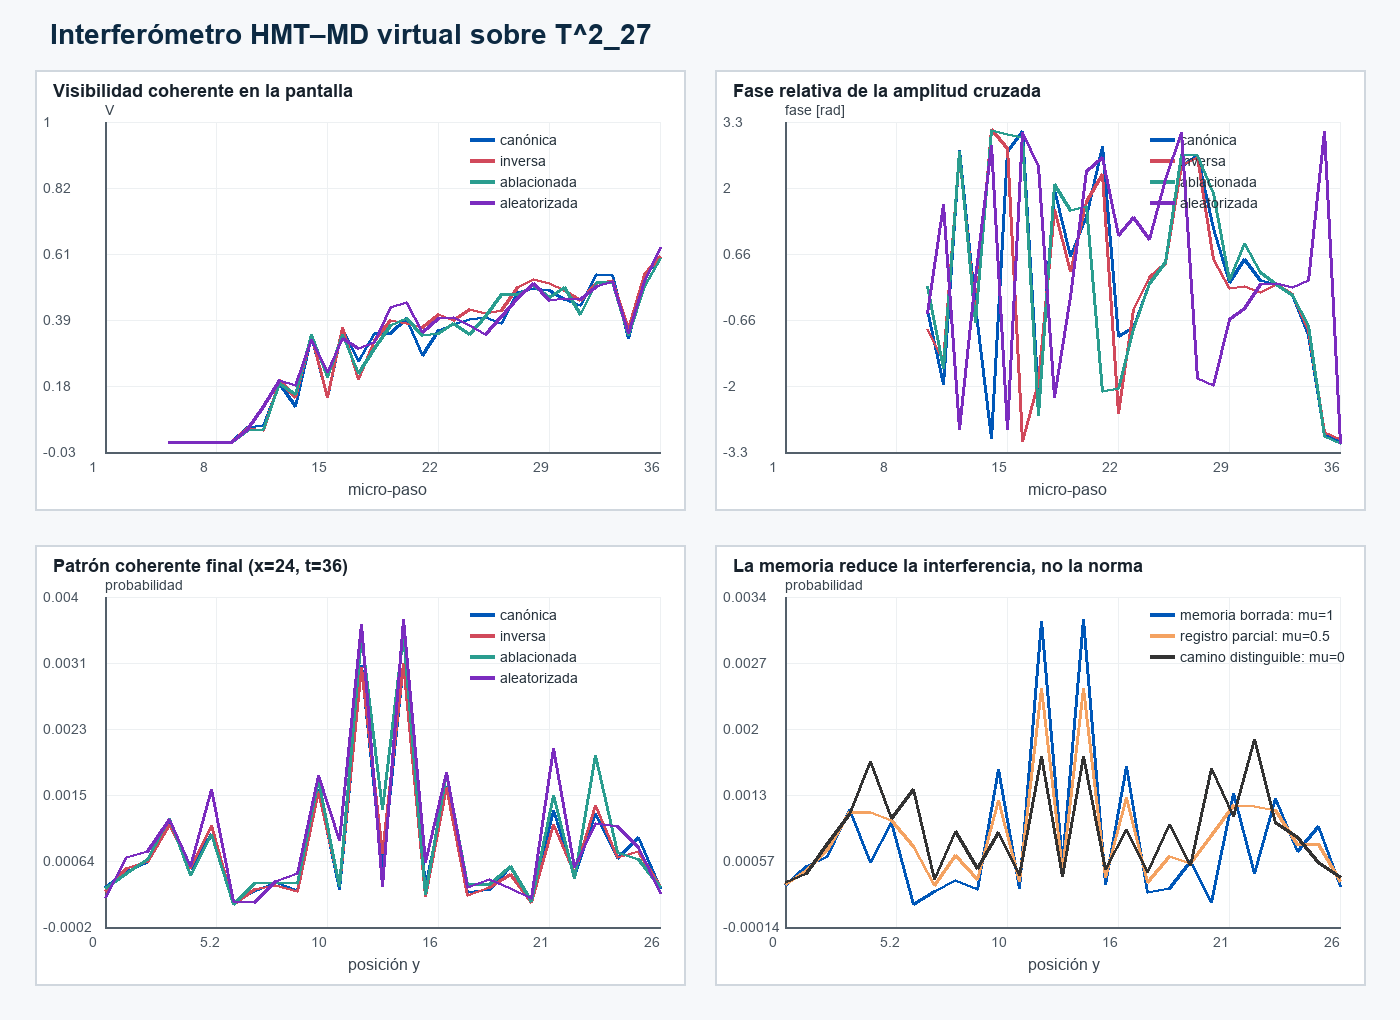
\includegraphics[width=.96\linewidth]{figures/parte_iv/01_curvas_y_patrones.png}
\caption[Evolution of visibility, relative phase, and final pattern]{Evolution of visibility, relative phase, and final pattern for the four sequences with common budget. The original image depicts the virtual HMT--MD interferometer on \(T^2_{27}\). Panel labels, from left to right and top to bottom: coherent visibility on the screen; relative phase of the cross amplitude; final coherent pattern \((x=24,t=36)\); memory reduces interference, not the norm. Axes: microstep, position \(y\), phase in radians, and probability. The four sequences are canonical, inverse, ablated, and randomized. The memory curves represent erased memory \((\mu=1)\), partial record \((\mu=0.5)\), and a distinguishable path \((\mu=0)\).}
\label{fig:md-sucesora-interferometro-patrones}
\end{figure}

\begin{figure}[tbp]
\centering
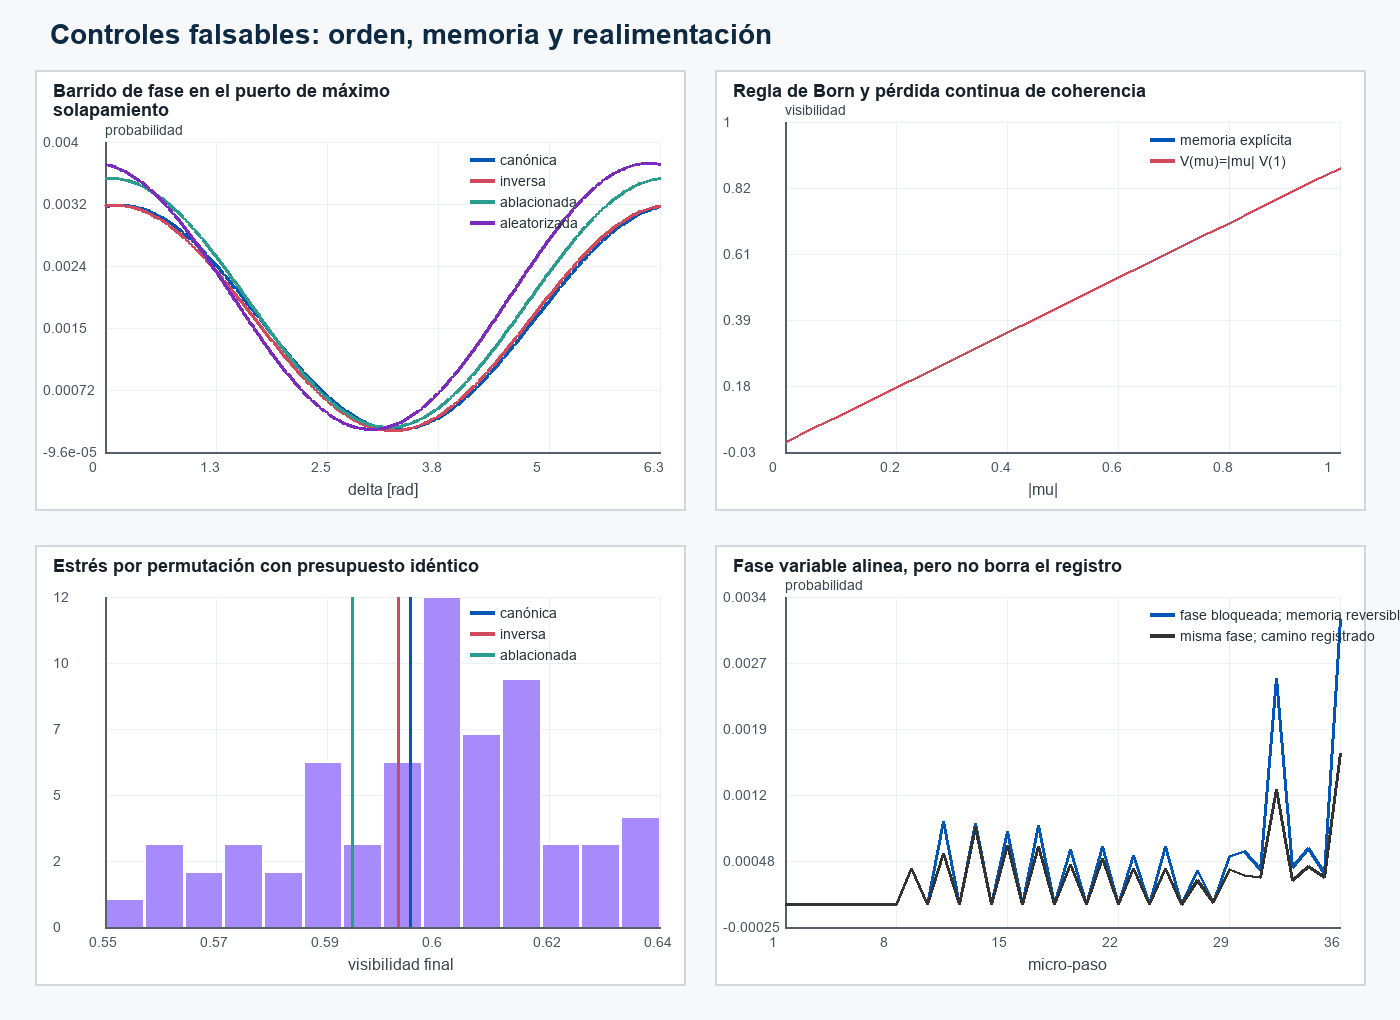
\includegraphics[width=.96\linewidth]{figures/parte_iv/02_estres_memoria_y_control.png}
\caption[Order controls, path memory, and phase feedback]{Order controls, path memory, and phase feedback. The original image presents falsifiable controls of order, memory, and feedback. Panel labels, from left to right and top to bottom: phase sweep at the port of maximum overlap; Born rule and continuous loss of coherence; permutation stress with an identical budget; variable phase aligns, but does not erase the record. Axes: probability, visibility, \(\delta\) in radians, \(|\mu|\), final visibility, and microstep. Sequence labels: canonical, inverse, ablated, and randomized. The other curves denote explicit memory, \(V(\mu)=|\mu|V(1)\), locked phase with reversible memory, and the same phase with a recorded path.}
\label{fig:md-sucesora-interferometro-controles}
\end{figure}

\endgroup

\begingroup
\def\HMTDesiredChapterTitle{Quantum Occupation Statistics: Fermi--Dirac and Bose--Einstein Distributions}%
\let\HMTOriginalChapter\chapter
\renewcommand{\chapter}[2][]{\HMTOriginalChapter{\HMTDesiredChapterTitle}}%
\chapter{Quantum Occupation Statistics: Fermi–Dirac and Bose–Einstein Distributions}
\label{chap:parte-iv-55}

Microcanonical enumeration and the symmetric and antisymmetric completions produce the Bose--Einstein and Fermi--Dirac laws. The Maxwell--Boltzmann limit is retained as a derived regime, not as a starting point.

\section{Microcanonical enumeration of states on a finite screen}

Consider the finite realization
\[
 \mathcal H_{\rm occ}=\bigoplus_{k=0}^{3}\CC^{g_k},
 \qquad
 H_{\rm occ}|_{\CC^{g_k}}=E_k^{\rm occ} I,
\]
with levels and multiplicities
\[
 E^{\rm occ}=(0,3,6,9),\qquad g=(1,6,12,8),
 \qquad(N,E)=(12,66).
\]
The sum \(1+6+12+8=27\) makes \(\mathcal H_{\rm occ}\) a screen of
twenty-seven modes. This spectrum is the datum of a declared finite
representation; its cardinality does not suffice to identify it with any other
occurrence of \(27\) in HMT\@. The morphism relating a specific
boundary screen to \((\mathcal H_{\rm occ},H_{\rm occ})\) must specify both
the fibers and the spectral operator.
The fermionic and bosonic generating functions are
\[
 F(y,x)=\prod_k(1+yx^{E_k^{\rm occ}})^{g_k},
 \qquad
 B(y,x)=\prod_k(1-yx^{E_k^{\rm occ}})^{-g_k}.
\]

\begin{proposition}[Microcanonical cardinalities]
\label{prop:cardinalidades-microcanonicas}
\[
 [y^{12}x^{66}]F=2\,104\,494,
 \qquad
 [y^{12}x^{66}]B=259\,436\,430.
\]
\end{proposition}
\begin{proof}
In the fermionic product, choosing \(r\) of the \(g_k\) modes contributes
\(\binom{g_k}{r}y^rx^{rE_k^{\rm occ}}\). In the bosonic product, distributing \(r\)
indistinguishable occupations among \(g_k\) modes contributes
\(\binom{g_k+r-1}{r}y^rx^{rE_k^{\rm occ}}\). The finite convolution over the
four levels produces the stated integers.
\end{proof}

\section{Bose--Einstein and Fermi--Dirac distributions}

The equilibrium formulation starts from the Hamiltonian and the total
occupation number,
\begin{equation}
 H=\sum_kE_k^{\rm occ} n_k,
 \qquad
 N=\sum_k n_k,
 \qquad
 K_\mu:=H-\mu N.
 \label{eq:hamiltoniano-gran-canonico-rev3}
\end{equation}
For \(\beta>0\), the grand canonical state is
\begin{equation}
 \rho_{\beta,\mu}
 =\frac{e^{-\beta K_\mu}}{\mathcal Z_{\beta,\mu}},
 \qquad
 \mathcal Z_{\beta,\mu}
 =\operatorname{Tr}(e^{-\beta K_\mu}).
 \label{eq:estado-gran-canonico-rev3}
\end{equation}

\begin{theorem}[Grand canonical factorization and occupation laws]
\label{thm:factorizacion-gran-canonica-rev3}
For energy levels \(E_k^{\rm occ}\) with degeneracies \(g_k\), the
fermionic trace factorizes as
\begin{equation}
 \mathcal Z_{\rm FD}
 =\prod_k\bigl(1+e^{-\beta(E_k^{\rm occ}-\mu)}\bigr)^{g_k},
 \qquad
 \langle n_k\rangle_{\rm FD}
 =\frac{g_k}{e^{\beta(E_k^{\rm occ}-\mu)}+1}.
 \label{eq:factorizacion-fd-rev3}
\end{equation}
In the bosonic sector, under the condition
\(\mu<\inf_kE_k^{\rm occ}\),
\begin{equation}
 \mathcal Z_{\rm BE}
 =\prod_k\bigl(1-e^{-\beta(E_k^{\rm occ}-\mu)}\bigr)^{-g_k},
 \qquad
 \langle n_k\rangle_{\rm BE}
 =\frac{g_k}{e^{\beta(E_k^{\rm occ}-\mu)}-1}.
 \label{eq:factorizacion-be-rev3}
\end{equation}
\end{theorem}

\begin{proof}
The operator \(K_\mu\) is a sum of commuting occupation operators, so
its trace factorizes over modes. In each fermionic mode, the
occupations \(0\) and \(1\) are summed, and the corresponding factor is
\(1+u_k\), where
\(u_k=e^{-\beta(E_k^{\rm occ}-\mu)}\). In each bosonic mode, all
nonnegative occupations are summed, giving the geometric series
\((1-u_k)^{-1}\); the condition on \(\mu\) ensures \(u_k<1\). The
powers \(g_k\) incorporate the degeneracy. Finally,
\[
 \langle n_k\rangle
 =-\frac1\beta\frac{\partial}{\partial E_k^{\rm occ}}
   \log\mathcal Z
\]
yields the two occupation laws
\cite{Bose1924,Einstein1924,Fermi1926,Dirac1926,Pathria2011}.
\end{proof}

The microcanonical derivation recovers the same result in the
thermodynamic regime. For mean fermionic occupations
\(p_k=m_k/g_k\), the combinatorial entropy per level is
\begin{equation}
 S_k\simeq
 g_k\bigl[-p_k\log p_k-(1-p_k)\log(1-p_k)\bigr].
 \label{eq:entropia-fd-nivel-rev3}
\end{equation}
The variation of \(\sum_kS_k\), subject to
\(\sum_kg_kp_k=N\) and
\(\sum_kg_kE_k^{\rm occ}p_k=E\), gives
\begin{equation}
 \log\frac{1-p_k}{p_k}=\alpha+\beta E_k^{\rm occ},
 \qquad
 \mu=-\frac{\alpha}{\beta},
 \label{eq:variacion-fd-rev3}
\end{equation}
and hence the Fermi--Dirac occupation of
\eqref{eq:factorizacion-fd-rev3}. The multipliers \(\beta\) and \(\mu\)
are the dual coordinates of the energy and population constraints.

For mean bosonic occupations
\(\overline n_k=m_k/g_k\), the log-multiplicity of the level is
\begin{equation}
 S_k\simeq
 g_k\bigl[(1+\overline n_k)\log(1+\overline n_k)
          -\overline n_k\log\overline n_k\bigr].
 \label{eq:entropia-be-nivel-rev3}
\end{equation}
The variation of \(\sum_kS_k\), subject to
\(\sum_kg_k\overline n_k=N\) and
\(\sum_kg_kE_k^{\rm occ}\overline n_k=E\), yields
\begin{equation}
 \log\frac{1+\overline n_k}{\overline n_k}
 =\alpha+\beta E_k^{\rm occ},
 \qquad
 \overline n_k
 =\frac{1}{e^{\beta(E_k^{\rm occ}-\mu)}-1},
 \qquad
 \mu=-\frac{\alpha}{\beta}.
 \label{eq:variacion-be-rev3}
\end{equation}
This is the Bose--Einstein occupation of
\eqref{eq:factorizacion-be-rev3}. The condition
\(\mu<\inf_kE_k^{\rm occ}\) ensures positivity of the denominator and
convergence of each modal factor.

In the finite instance constructed, the two constraints determine
\[
 (\beta_{\rm FD},\mu_{\rm FD})
 =(0.15307011353415928,\,4.502865197597043),
\]
\[
 (\beta_{\rm BE},\mu_{\rm BE})
 =(0.05456727960068316,\,-15.92569781906737).
\]
If \(m_k^{\rm mic}\) denotes the mean occupancy obtained by exact
microcanonical enumeration and \(m_k^{\rm eq}\) the evaluation of the corresponding
distribution, the errors
\(\sum_k|m_k^{\rm mic}-m_k^{\rm eq}|\) are
\[
 0.09897380039002812\quad\hbox{and}\quad
 0.9190625715582017,
\]
respectively. The enumeration traverses all occupation quadruples,
computes their integer multiplicities, and solves the two constraint
equations. The two laws are realized on the same screen. The physical choice
between them requires a grading and a Hamiltonian compatible with the
trajectory representation. The thermal parameter will subsequently be typed
as \(\beta=(k_B\Theta)^{-1}\).

\section{Quantified convergence to the Maxwell--Boltzmann distribution}

The relation between the two quantum statistics and the classical regime can
be formulated without resorting to an informal approximation. For each mode, let
\[
 u_k:=e^{-\beta(E_k^{\rm occ}-\mu)}.
\]
The state occupations are written
\[
 \overline n_k^{\rm FD}=\frac{u_k}{1+u_k},
 \qquad
 \overline n_k^{\rm BE}=\frac{u_k}{1-u_k};
\]
the multiplicities \(g_k\) are incorporated subsequently through
\(\langle n_k\rangle=g_k\overline n_k\).

\begin{theorem}[Common classical limit of quantum statistics]
\label{thm:limite-clasico-fd-be-rev2}
If \(0\leq u_k\leq\delta<1\), then
\[
 \left|\overline n_k^{\rm FD}-u_k\right|\leq u_k^2,
 \qquad
 \left|\overline n_k^{\rm BE}-u_k\right|
 \leq\frac{u_k^2}{1-\delta}.
\]
Consequently, in the regime dilute \(u_k\to0\),
\[
 \boxed{
 \overline n_k^{\rm FD}\sim
 \overline n_k^{\rm BE}\sim
 e^{-\beta(E_k^{\rm occ}-\mu)}} ,
\]
which is the Maxwell--Boltzmann distribution per mode.
\end{theorem}

\begin{proof}
The exact identities
\[
 u_k-\frac{u_k}{1+u_k}=\frac{u_k^2}{1+u_k},
 \qquad
 \frac{u_k}{1-u_k}-u_k=\frac{u_k^2}{1-u_k}
\]
provide the bounds. For \(0<u_k\leq\delta\), dividing by \(u_k\) and
taking \(u_k\downarrow0\) yields
the asymptotic equivalence. The leading term of order \(u_k^2\) preserves the
physical difference: exclusion decreases fermionic occupation, whereas
accumulation increases bosonic occupation.
\end{proof}


\section{Quantum completions, leaf holonomy, and statistical periodicity}

The symmetric and exterior completions, the sheet grading, the holonomy
\(2\pi/4\pi\), the occupation counts, and the cellular complex of APP form a
single algebraic antecedent of quantum statistics. The complete development is incorporated here
so that periodicity is not reduced to a mere
subsequent reference.

\begingroup
\let\chapter\section
\let\section\subsection
\let\subsection\subsubsection
\let\subsubsection\paragraph
\let\clearpage\relax
\let\cleardoublepage\relax
\chapter{Statistical completions and fields over APP}
\label{chap:completaciones-cuanticas}

The words Bose, Fermi, Pauli, or photon do not by themselves designate theorems of a discrete system. Obtaining them requires specification of a state space, a grading, a product, and operators. APP and TPK provide a set of oriented states and a sheet parity. Two universal completions can be constructed from those data: the symmetric algebra and the exterior algebra. This section identifies exactly what follows from the construction and separates algebraic statistics from its physical interpretation.

\section{Linear state space associated with a particle realization}

Let \(S\) be a finite set of TPK route classes at the chosen depth,
and let
\[
 \mathcal H_1=\ell^2(S)
\]
be the Hilbert space with orthonormal basis \((e_s)_{s\in S}\). A choice of
positive weights \(E_s\) defines the diagonal operator
\[
 He_s=E_se_s.
\]
The choice of \(S\), its quotient by symmetries, and the weights are part
of the model. Once these are fixed, the multiparticle completions are canonical.

\section{Symmetric and exterior completions}

We define
\[
 \mathcal F_+(\mathcal H_1)=
 \bigoplus_{n\geq0}\operatorname{Sym}^n\mathcal H_1,
 \qquad
 \mathcal F_-(\mathcal H_1)=
 \bigoplus_{n\geq0}\bigwedge^n\mathcal H_1.
\]
The first is the bosonic completion; the second, the fermionic.

\begin{theorem}[Pauli exclusion principle in the exterior completion]
For every mode \(s\in S\), the creation and annihilation operators of the
exterior completion satisfy
\[
 \{a_s,a_t^\dagger\}=\delta_{st}I,
 \qquad
 \{a_s,a_t\}=\{a_s^\dagger,a_t^\dagger\}=0.
\]
In particular, the occupation operator
\(N_s=a_s^\dagger a_s\) is a projector:
\[
 N_s^2=N_s,
\]
and its eigenvalues are \(0,1\).
\end{theorem}

\begin{proof}
Creation is the exterior product by \(e_s\); annihilation is its
adjoint. Antisymmetry implies \(e_s\wedge e_s=0\) and yields the canonical
relations by calculation on the exterior basis. Then
\[
N_s^2=a_s^\dagger a_sa_s^\dagger a_s
=a_s^\dagger(I-a_s^\dagger a_s)a_s=N_s.
\]
Every self-adjoint projector has spectrum contained in \(\{0,1\}\).
\end{proof}

The exclusion principle thus appears as a theorem of the exterior
completion. The specifically HMT question is which transport datum selects
that completion for a class of routes.

\section{Sheet grading and exchange algebra}

Suppose that the oriented sheet defines an additive character
\[
 p:\operatorname{Mor}(\mathsf P_{\rm TPK})\longrightarrow\mathbb Z/2\mathbb Z,
 \qquad p(\gamma\eta)=p(\gamma)+p(\eta).
\]
On the corresponding graded linear space, introduce the symmetry
\[
 \tau(v\otimes w)=(-1)^{p(v)p(w)}w\otimes v.
\]

\begin{theorem}[Statistical completion determined by parity]
The quotient of the tensor algebra by the relations
\[
 v\otimes w-(-1)^{p(v)p(w)}w\otimes v
\]
is symmetric on the even sector and exterior on the odd sector. Two identical
odd states have zero product; even states admit arbitrary
occupation.
\end{theorem}

\begin{proof}
If \(p(v)=p(w)=0\), the relation is \(vw=wv\). If
\(p(v)=p(w)=1\), it is \(vw=-wv\); setting \(v=w\) and working in
characteristic zero gives \(v^2=0\). Mixed sectors commute without
an additional sign. This is the universal property of the graded symmetric
algebra.
\end{proof}

The theorem converts a compositional TPK parity into an exact occupancy
rule. To obtain the physical spin--statistics theorem, one must additionally
construct a positive local Lorentzian theory and prove that sheet parity
coincides with spin under rotations. The equality does not follow solely
from both objects taking values modulo two.

\section{Sheet holonomy and \texorpdfstring{\(2\pi/4\pi\)}{2pi/4pi} periodicity}

The preceding parity admits a natural geometric realization when a
surviving extension has a closed return with a nontrivial orientation
cover. Let \(\rho\) be the return generator and let
\[
 \varepsilon:\langle\rho\rangle\longrightarrow\{-1,+1\}
\]
be its holonomy character, with \(\varepsilon(\rho)=-1\). The associated real
bundle is then the orientation line of a Möbius strip: one
turn closes the geometric projection but changes the lifted sheet; two
turns restore the orientation.

To express this property in angular terms, fix a unitary
representation \(U\) of the rotation cover on the graded space
\(\mathcal H_1=\mathcal H_{\bar0}\oplus\mathcal H_{\bar1}\), compatible with
sheet parity in the sense that
\[
 U(2\pi)v=(-1)^{p(v)}v
\]
for every homogeneous vector \(v\). Compatibility is a condition of the
realization: it identifies the generator of the orientation cover with the
character \(p\) already constructed on the routes.

\begin{theorem}[Restoration of orientation and exchange algebra]
\label{thm:dos-cuatro-pi-estadistica}
Under the preceding compatibility condition,
\[
 U(2\pi)|_{\mathcal H_{\bar0}}=I,
 \qquad
 U(2\pi)|_{\mathcal H_{\bar1}}=-I,
 \qquad
 U(4\pi)=I.
\]
Moreover, the same character \(p\) determines the graded symmetry
\[
 \tau(v\otimes w)=(-1)^{p(v)p(w)}w\otimes v.
\]
Thus the even-holonomy sector is completed by symmetric
powers and the odd-holonomy sector by exterior powers. In
the latter, the exclusion relation \(v\wedge v=0\) holds.
\end{theorem}

\begin{proof}
The first and second equalities are the compatibility condition evaluated
on each homogeneous component. Iterating one turn gives
\[
 U(4\pi)v=U(2\pi)^2v=(-1)^{2p(v)}v=v,
\]
which proves the restoration. The assertion concerning exchange is the
parity-completion theorem of the preceding section: for two even vectors
the sign is positive, whereas for two odd vectors it is negative.
\end{proof}

Three returns should be distinguished. Angular closure after \(2\pi\) is a
return of the projection; closure after \(4\pi\) restores the lifted
orientation; neither, by itself, requires every coordinate of the record
to return to its initial value. This separation is the dimensional analogue of the
HMT distinction between phase return and state return.

\subsection{The sum and product sheets as supports of the \(2\) completions}

The APP table contains two evaluations on the same support. The
additive sheet acts by translations and preserves the multiplicity of
continuations; in this sense, it accumulates. The multiplicative sheet
permutes the units and contracts fibers over noninvertible elements; in
this sense, it folds. This incompatibility precedes the statistical
choice and explains why TPK must preserve two genealogies rather than
reduce them to a single visible word.

The statistical assignment is not obtained, however, by verbally replacing
``sum'' with ``boson'' and ``product'' with ``fermion.'' The exact map is
the parity character
\[
 p:\operatorname{Mor}(\mathsf P_{\rm TPK})\longrightarrow\mathbb Z/2\mathbb Z.
\]
When the transport of an extension lies in the sector \(p=0\), its
completion admits cumulative occupation and is symmetric. When it lies in
\(p=1\), sheet reversal introduces the exchange sign and the
completion is exterior. Sum and product supply the two
local geometries; the record, orientation, and character \(p\) determine the
sector in which a route is realized.

With a diagonal Hamiltonian \(H\), energy \(\epsilon\), chemical potential
\(\mu\), and thermal parameter \(\beta\), the mean occupations of the two
sectors are then
\[
 \bar n_{\rm par}(\epsilon)
 =\frac{1}{e^{\beta(\epsilon-\mu)}-1},
 \qquad
 \bar n_{\rm impar}(\epsilon)
 =\frac{1}{e^{\beta(\epsilon-\mu)}+1}.
\]
The Bose--Einstein and Fermi--Dirac formulas are therefore the
thermodynamic evaluations of the symmetric and exterior completions
selected by transport. The periodicity \(4\pi\) and fermionic
exclusion are coordinated by the same character, but neither of them
is inferred from a mere numerical coincidence.

\section{Number and Occupation Distribution Operators in the Fock Realization}

If there are \(g\) modes and \(N\) particles, the sector dimensions are
\[
 \Omega_F(g,N)=\binom gN,
 \qquad
 \Omega_B(g,N)=\binom{g+N-1}{N}.
\]
The first formula counts subsets of modes; the second, weak compositions of
\(N\) into \(g\) parts. These counts are exact consequences of
the two completions and require no thermodynamic hypothesis.

\section{The cellular complex of the APP torus}

The APP graph is the one-skeleton of a cellular decomposition of the torus
\(T^2\) with \(9\times9\) vertices. Let
\[
 C^0\xrightarrow{d_0}C^1\xrightarrow{d_1}C^2
\]
be its real cochain complex. Choosing the uniform inner product,
define the codifferential \(\delta=d^*\) and the Laplacian
\[
 \Delta_k=d_{k-1}\delta_k+\delta_{k+1}d_k.
\]

\begin{theorem}[Harmonic sector of the digital torus]
The dimension of the space of harmonic one-forms is two:
\[
 \dim\ker\Delta_1=b_1(T^2)=2.
\]
A basis can be chosen that is represented by the uniform horizontal and
vertical flows. Both are closed and coclosed, and neither is the gradient of
a globally defined periodic function.
\end{theorem}

\begin{proof}
The Hodge theorem for finite cellular complexes identifies
\(\ker\Delta_1\) with \(H^1(T^2;\mathbb R)\). The cohomology of the torus has
rank two. Directly, the constant horizontal and vertical flows have
zero divergence and curl; their integrals over the two fundamental
cycles are independent, so they are not exact.
\end{proof}

The space of connections modulo gauge transformations is
\[
 C^1/\operatorname{im}d_0.
\]
In a finite complex equipped with the preceding inner product, each orbit
admits a Coulomb representative in \(\ker\delta_1\); within the orbit,
the choice is unique modulo the stabilizer \(\ker d_0\) of the gauge
parameter. The correct cohomological quotient is
\[
 \ker d_1/\operatorname{im}d_0
 \simeq \ker\Delta_1 .
\]
Its two harmonic classes constitute a natural mathematical candidate for
two free global modes. They are not yet the two local polarizations of
a photon in \(3+1\)-dimensional spacetime: that identification requires a
dynamical limit, a dispersion relation, and a physical gauge group.

\section{Discrete Gauss law}

For an oriented 1-cochain \(F\) and a set of vertices \(V\),
divergence is defined by
\[
 (\operatorname{div}F)(v)=
 \sum_{e:v\to w}F(e)-\sum_{e:w\to v}F(e).
\]
Summing over \(V\), every interior edge appears once with each sign and
cancels. Therefore,
\[
 \boxed{
 \sum_{v\in V}\operatorname{div}F(v)
 =\operatorname{Flux}_{\partial V}(F).}
\]
This identity is an exact Gauss law on the graph. Interpreting
\(\operatorname{div}F\) as electric charge requires the charge character and
dimensional realization constructed in Dimensional Mechanics.

\section{Reversible measurement apparatus}

Let \(S\) be a set of states and let \(r:S\to\mathbb Z/9\mathbb Z\) be a
readout. Coupling to a nonadic register is defined by
\[
 U_r:S\times\mathbb Z/9\mathbb Z\longrightarrow
 S\times\mathbb Z/9\mathbb Z,
 \qquad
 U_r(s,a)=(s,a+r(s)).
\]

\begin{proposition}[Reversibility of the coupling]
The map \(U_r\) is to permutation and
\[
 U_r^{-1}(s,a)=(s,a-r(s)).
\]
Information loss arises only after applying a reader to the
register or conditioning the state on the outcome.
\end{proposition}

\begin{proof}
The proposed inverse satisfies both composition identities by the
group law of \(\mathbb Z/9\mathbb Z\).
\end{proof}

This proposition formalizes the operational definition of measurement: coupling,
reading, and restricting compatible futures are three different maps. The
full coupling is reversible; the observational quotient need not be.

\section{Algebraic correspondences and physical realizations}

The Fock completions, exclusion conditional on parity, the harmonic
sector of APP, discrete Gauss law, and reversibility of the apparatus are complete
mathematical theorems. Their physical identifications form a diagram that
must commute:
\[
 \text{sheet parity}
 \longrightarrow\text{graded interchange}
 \longrightarrow\text{CAR/CCR}
 \longrightarrow\text{physical statistics},
\]
\[
 H^1(\mathcal A_9)
 \longrightarrow\text{discrete gauge field}
 \longrightarrow\text{massless mode}
 \longrightarrow\text{photon}.
\]
The first two arrows of each line have explicit constructions; the
last require the corresponding dynamics and physical limit. This
separation permits the bridges to be developed without conflating an analogy of
cardinality with a representation.

\endgroup

\paragraph{From reversible measurement to fermionic occupation and to the algebraic exclusion principle of Pauli} The statistical distinction is completed algebraically through occupation idempotence and fermionic exclusion.

\endgroup
% Contenido exclusivo del propietario de entropías tipadas.
\subsection{Quasi-free correlation and spectral occupation entropies}

For a gauge-invariant, number-conserving quasifree fermionic state
defined on a finite-dimensional one-particle space, let
\(C_{ij}=\langle a_j^\dagger a_i\rangle\) be the one-particle correlation
operator. The gauge-invariant hypothesis excludes anomalous pairing
correlations, so that \(C\) determines the quasifree state. If
\(0<C<I\), its one-particle modular generator and the reciprocal reconstruction
of the correlator are
\begin{equation}
 \boxed{
 K_1=\log\bigl((I-C)C^{-1}\bigr),
 \qquad
 C=(I+e^{K_1})^{-1}.}
 \label{eq:puente-cuasilibre-modular-rev3}
\end{equation}

\begin{corollary}[Logistic form of the modular spectrum]
\label{cor:forma-logistica-modular-rev3}
If \(K_1u_i=\kappa_i u_i\), the occupation of mode \(u_i\) is
\[
 \langle n_i\rangle=\frac1{1+e^{\kappa_i}}.
\]
For \(\kappa_i=\beta(\varepsilon_i-\mu)\), the Fermi--Dirac law
is recovered.
\end{corollary}

\begin{proof}
The spectral diagonalization of \(K_1\) diagonalizes every function thereof. Applying
\(x\mapsto(1+e^x)^{-1}\) to each eigenvalue yields the formula.
\end{proof}

If \(C\) has eigenvalues \(p_i\in[0,1]\), the occupation entropy of the
quasifree fermionic state is, with the convention \(0\log0=0\),
\begin{equation}
 S_F=-\sum_i\bigl[p_i\log p_i+(1-p_i)\log(1-p_i)\bigr].
 \label{eq:entropia-cuasilibre-fermi-rev3}
\end{equation}
For a diagonal Gaussian bosonic state with finitely many modes and mean
occupancies \(\overline n_i\),
\begin{equation}
 S_B=\sum_i\bigl[(1+\overline n_i)\log(1+\overline n_i)
                  -\overline n_i\log\overline n_i\bigr].
 \label{eq:entropia-gaussiana-bose-rev3}
\end{equation}
The same formula extends to a countable family when the series on the
right-hand side converges.
These entropies quantify occupation configurations. Entanglement entropy
has another domain: the reduced state induced by a tensor
decomposition. Identifying the two requires specifying the reduction and the
correlation operator that implements it.

Finally, for a reduced state \(\rho_A\), the \emph{von Neumann
entropy}
\[
 S_{\rm vN}(\rho_A)=-\operatorname{Tr}(\rho_A\log\rho_A)
\]
is a spectral property of the density operator. When \(\rho_A\)
comes from a global purification, it quantifies entanglement across
the cut. In the HMT boundary construction, the area operator, the
modular Hamiltonian, and the corresponding reduction remain in the
\cref{hap:sec:area-entrelazamiento-barbero-rev11}.

The maps between these domains are published through explicit identities.
The decomposition of a measure along the fibres of \(q\) satisfies the chain
rule
\begin{equation}
 \mathsf H_\mu(\mathbf X)
 =\mathsf H_{q_*\mu}(q(\mathbf X))
  +\mathsf H_{\rm fib}(q;\mu).
 \label{eq:cadena-entropia-fibras-rev2}
\end{equation}
\Needspace{5\baselineskip}
A finite distribution \(p=(p_i)\) is realized diagonally as
\[
 \rho_p=\sum_i p_i|i\rangle\langle i|,
 \qquad S_{\rm vN}(\rho_p)=\mathsf H(p).
\]
If \(P_{N,E}\) projects onto the microcanonical subspace of dimension
\(\Omega(N,E)\), then
\[
 \rho_{\rm mc}=\frac{P_{N,E}}{\Omega(N,E)},
 \qquad S_{\rm vN}(\rho_{\rm mc})=\log\Omega(N,E)=S_{\rm mc}.
\]
For a pure bipartite state,
\[
 \rho_A=\operatorname{Tr}_B
 \bigl(|\Psi_{AB}\rangle\langle\Psi_{AB}|\bigr)
\]
defines the reduction that measures entanglement. Finally, equality between
\(h_{\rm top}=\log\rho(A)\) and a metric entropy is attained, for this
primitive system, by means of the Parry measure, which realizes maximal metric
entropy; it is not attributed to an arbitrary measure on histories.



\begingroup
\def\HMTDesiredChapterTitle{Fermionic completion of paths and Pauli's algebraic exclusion principle}%
\let\HMTOriginalChapter\chapter
\renewcommand{\chapter}[2][]{\HMTOriginalChapter{\HMTDesiredChapterTitle}}%
\chapter{Fermionic completion of paths and Pauli's algebraic exclusion principle}
\label{chap:parte-iv-56}

Exterior completion of the trajectories imposes idempotence and exclusion before any species identification. The rotation, color, flavor, and virtuality characters preserve their typing within the corresponding representation.

\section{Occupation, exclusion and finite statistics}
\label{chap:ocupacion-estadistica}
\index{Pauli exclusion principle}\index{CAR}
\index{Fermi--Dirac}\index{Bose--Einstein}

The null and material realizations provide the geometric support of occupation. The fermionic sector is constructed on the canonical anticommutation relations (CAR), and the spin--statistics theorem further requires the declared operator representation. This section fixes those premises before deriving idempotence of occupation, the microcanonical cardinalities, and the Bose--Einstein and Fermi--Dirac distributions with their common classical limit.

\subsection{Idempotency of Occupation in the Anticommutation Algebra}

Let \(a_i,a_i^\dagger\) be operators satisfying the canonical
anticommutation relations (CAR)
\[
 \{a_i,a_j^\dagger\}=\delta_{ij},
 \qquad \{a_i,a_j\}=0,
\]
and let \(n_i=a_i^\dagger a_i\).

\begin{theorem}[Pauli Exclusion Principle]
\label{thm:principio-exclusion-pauli}
One has \(n_i^2=n_i\), and therefore
\(\Spec(n_i)\subseteq\{0,1\}\).
\end{theorem}
\begin{proof}
\[
 n_i^2=a_i^\dagger a_i a_i^\dagger a_i
 =a_i^\dagger(1-a_i^\dagger a_i)a_i
 =a_i^\dagger a_i,
\]
because \(a_i^2=(a_i^\dagger)^2=0\). Every eigenvalue of an idempotent
satisfies \(\lambda^2=\lambda\) \cite{Pauli1925,Dirac1926}.
\end{proof}

The nilpotence \((a_i^\dagger)^2=0\) precludes double fermionic occupation of the
same mode and, upon maximizing entropy under the energy and number
constraints, leads to the Fermi--Dirac occupation law presented below.
The symmetric completion and the Bose--Einstein law constitute a distinct
stratum and are presented separately.

The CAR relations are an algebraic hypothesis of the theorem. A monodromy
with sign change under a rotation of \(2\pi\) is compatible with a
fermionic representation, but does not by itself constitute a derivation of
CAR or of the spin--statistics theorem.


\section{Spin, color, flavor, and virtuality characters}

Let \(\jmath:\Gamma_{\rm TPK}\to\Gamma_{\rm TPK}\) be the involution that reverses
the orientation of each edge and permutes the fibers through
\(J_c:E_c\to E_{\jmath c}\). A spin character is a representation
\(\rho_{\rm rot}\) of the subgroup generated by \(\jmath\) on the sections;
its sign eigenspaces \(+1\) and \(-1\) are algebraic objects distinct
from a physical representation of the Lorentz group.

Let \(\mathcal C\) be the Abelian group of channel characters of the transport.
Two sections have the same \emph{arithmetic flavour} when their characters
\[
 \chi_s:\mathcal C\longrightarrow\CC^\times
\]
coincide. Identifying these classes with fermion flavors requires
a representation of the algebra of physical observables and is not introduced by
nomenclature.

Finally, let
\[
 \operatorname{Ext}_N(s)=
 \{s'\in\Gamma(\mathcal B_{\gamma'}):
 \gamma'|_{\{0,\ldots,N\}}=\gamma,\ s'|_{\{0,\ldots,N\}}=s\}.
\]
The section is stable from depth \(N\) onward when the restrictions
\(\operatorname{Ext}_{N+1}(s)\to\operatorname{Ext}_N(s)\) admit a compatible branch
at every subsequent level. It is called \emph{virtual up to
depth \(N\)} when that global branch does not yet exist, although
finite extensions survive. This definition belongs to the inverse system and does not
depend on a temporal metaphor.

On the affine plane \(\FF_3^2\), the linear functional
\[
 \kappa_3:\FF_3^2\longrightarrow\FF_3,
 \qquad \kappa_3(r,c)=r-c
\]
is surjective, and its kernel has dimension one. Consequently, its three
fibers are the affine classes of the kernel, and each contains exactly three
points. The same balance persists in every disjoint union of complete
copies of \(\FF_3^2\). This ternary partition is a self-contained algebraic
statement. Once the qutrit chart, the orientation, and the phase character have been fixed,
the \cref{chap:algebra-color-qutrit} constructs the representation and its algebra
\(\mathfrak{su}(3)\); the intertwiner with TPK transport and the physical
chromodynamic identification remain an interface.


\paragraph{Distinction between reversible genealogical transport and irreversible projection.} Reversibility of the update permits the cost of an irreversible projection to be distinguished from complete genealogical transport.

\endgroup

\begingroup
\def\HMTDesiredChapterTitle{Reversible update, deletion cost, and exact domain of the Landauer null limit}%
\let\HMTOriginalChapter\chapter
\renewcommand{\chapter}[2][]{\HMTOriginalChapter{\HMTDesiredChapterTitle}}%
\chapter{Reversible update, deletion cost, and exact domain of the Landauer null limit}
\label{chap:parte-iv-57}

The full transport preserves fibre information and may have zero logical cost; the projection or reinitialization that discards the genealogy is subject to Landauer's cost. The two domains are separated explicitly.

\section{Logical reversibility and Landauer's principle in TPK fibers}
\label{sec:informacion-fibra-landauer-rev7}
\index{Landauer's principle}\index{information!fiber}

Let \((\Omega,2^\Omega,\mu)\) be a finite probability space, let
\(X:\Omega\to\mathcal X\) be a random variable with values in the space
\(\mathcal X\) of complete states, and let \(q:\mathcal X\to Y\) be a reader.
The chain rule gives
\[
 \mathsf H(X)
 =
 \mathsf H(q(X))+\mathsf H(X\mid q(X)).
\]
The second summand measures the information of the fiber that the reader does not
publish.

\begin{theorem}[Landauer zero for full transport and projection cost]
\label{thm:landauer-relativo-lector-rev7}
If \(U:\mathcal X\to\mathcal X\) is a bijective update of the complete
HMT state,
then
\[
 \boxed{\mathsf H(X\mid U(X))=0.}
\]
For a projected output \(q(U(X))\), the discarded information is
\[
 \mathsf H(X\mid q(U(X))).
\]
A physical reset that identifies distinct memory states must
account for that information in the environment.
\end{theorem}

\begin{proof}
Bijectivity implies
\(X=U^{-1}(U(X))\); therefore \(X\) is determined by \(U(X)\) and the
conditional entropy is zero. For the reader \(q\), the chain rule
separates published entropy from fiber entropy. If the reset operation is
not injective, the output no longer permits reconstruction of the memory
state. Landauer's thermodynamic principle bounds the cost of implementation in
terms of that erased entropy; the reversible update does not by itself
contribute an erasure term.
\end{proof}

In nats and bits, respectively,
\[
 Q\ge k_B\Theta\,\mathsf H_{\rm nat},
 \qquad
 Q\ge k_B\Theta\log 2\,\mathsf H_{\rm bit}.
\]
For bijective transport of the complete state, the erasure entropy is
zero and, therefore, the minimum Landauer term associated exclusively with
erasure satisfies
\[
\boxed{Q_{\rm L}^{\min}[U]=k_B\Theta\,
 \mathsf H(X\mid U(X))=0.}
\]
For the restart of a uniform TRIT, on the other hand,
\[
 \boxed{Q_{\rm reset}\ge k_B\Theta\log3.}
\]
These two equations locate the cost in information loss: the cost appears when projection or resetting forgets the fiber. Preparation, projection, and resetting may produce entropy; reversible transport preserves genealogical information. The null value is the logical Landauer limit for that complete update, whereas the dynamical costs of control, finite speed, and coupling to the environment belong to the physical realization of the device.

\begin{statusbox}[title={Scope of the null Landauer relation}]
The equality \(\mathsf H(X\mid U(X))=0\) is exact for a bijective update of the enriched state. The bound \(Q_{\rm reset}\ge k_B\Theta\log3\) is the Landauer specialization to the erasure of a uniform triadic decision. Realizing both formulas in joules uses the Boltzmann transducer and a declared physical temperature.
\end{statusbox}


\paragraph{Edge Information Transduction in Minimum Triadic Cut Capacity.} The information preserved by the boundary reappears geometrically in the minimal triadic cut and in its capacity.

\endgroup
\begingroup
\let\HMTOwnerSection\section
\let\HMTOwnerSubsection\subsection
\let\HMTOwnerSubsubsection\subsubsection
\let\HMTOwnerParagraph\paragraph
\let\chapter\HMTOwnerSection
\let\section\HMTOwnerSubsection
\let\subsection\HMTOwnerSubsubsection
\let\subsubsection\HMTOwnerParagraph
\chapter{Genealogical Conservation of Information, Reduction Entropies and Thermal Structure}
\label{chap:informacion-entropia-landauer}

The information transported by an HMT state is not exhausted by the coordinate that
one of its readers publishes. The visible coordinate, sheet, orientation,
quotient, carry, route, and closure seal belong to the same
enriched state, even though a particular evaluation displays only part of
it. This distinction makes it possible to place in a single framework three operations that the
macroscopic description usually presents separately: preserving a history,
reducing it to a reading, and assigning energy to the information actually
erased.

The chapter develops that chain without identifying its stages. It first
formulates fiber memory and the exact recoverability criterion. It then
proves the vanishing of the logical Landauer term for a bijective update
of the TPK enriched state. Five entropies having different domains and
functions are subsequently distinguished. Finally, the areal--volumetric quotient
and the clock of \(108\) steps provide the structure that
links triadic information, action, and temperature.

\section{Disintegration of Visible Reading Over Fibers and Recovery of Genealogical Memory}

Let \(\Omega\) be a finite space of enriched states, and let
\[
 q:\Omega\longrightarrow Y
\]
a visible reader. The value \(q(x)\) is a coordinate of the state \(x\), not its
exhaustive description. Denote by
\[
 M:\Omega\longrightarrow\mathcal M
\]
the joint record of the genealogical coordinates that the reader does not publish:
leaf, orientation, quotient or carry, phase, route, and seal, according to the
domain under consideration.

\begin{definition}[Enhanced reader and fiber memory]
The enriched reader associated with \(q\) and \(M\) is
\begin{equation}
 \widehat q=(q,M):\Omega\longrightarrow Y\times\mathcal M.
 \label{eq:lector-enriquecido-informacion}
\end{equation}
The fibre memory of \(q\) is the information needed to distinguish the
states contained in the same fibre \(q^{-1}(y)\).
\end{definition}

The APP residue--quotient extension is the elementary arithmetic example. In
each cell, both Euclidean divisions are preserved
\[
 i+j=9q^+_{ij}+R^+_{ij},
 \qquad
 ij=9q^\times_{ij}+R^\times_{ij}.
\]
Reduction modulo nine publishes \(R^+\) or \(R^\times\); the lift
simultaneously preserves \((R,q)\). Summing over the nonadic domain yields
the exact identity
\begin{equation}
 2025-810
 =54+9\cdot129.
 \label{eq:app-residuo-cociente-informacion}
\end{equation}
The first term on the right is the difference between the visible residues;
the second recomposes the difference between the quotients. The equality
shows that the residual projection does not by itself determine the integral
operation.

Now let \(X\) be a random variable with values in \(\Omega\). We shall work
with dimensionless entropies in nats. The chain rule gives
\begin{equation}
 \mathsf H(X)
 =\mathsf H(q(X))+\mathsf H(X\mid q(X)).
 \label{eq:cadena-entropia-fibra}
\end{equation}
The second term quantifies the genealogical information that remains within
the fiber of the reading.

\begin{theorem}[Fiber Memory Recoverability]
\label{thm:recuperabilidad-memoria-fibra}
If the enriched reader \(\widehat q=(q,M)\) is injective on the support of
\(X\), then
\begin{equation}
 \boxed{\mathsf H(X\mid q(X),M(X))=0.}
 \label{eq:entropia-condicional-memoria-cero}
\end{equation}
The entropy \(\mathsf H(X\mid q(X))\) measures exactly the information that would be
lost by retaining the visible coordinate and discarding the memory.
\end{theorem}

\begin{proof}
The injectivity of \(\widehat q\) provides an inverse on its image. Hence the
pair \((q(X),M(X))\) determines \(X\), and the conditional entropy is
zero. If \(M(X)\) is omitted, entries in the same fiber are identified;
the chain rule \eqref{eq:cadena-entropia-fibra} assigns the term \(\mathsf H(X\mid q(X))\) to that
identification.
\end{proof}

The genealogical definition of number enters precisely here. An HMT number
is a compatible section of surviving cylinders together with the memory
of its route, orientation, signature, and closure. Its real value is the evaluation of that
section. Evaluation may forget coordinates; the section preserves them.

\section{Logical reversibility and Landauer's term}

Let
\[
 U:\Omega\longrightarrow\Omega
\]
an update of the enriched TPK state. Landauer's question is posed on the
complete map, before a visible reader is applied or a record is reset; its
thermodynamic formulation of logical erasure dates to Landauer
\cite{Landauer1961}.

\begin{theorem}[Landauer zero for full transport]
\label{thm:landauer-nulo-tpk-anexo}
If \(U\) is bijective, then, for every input distribution \(X\),
\begin{equation}
 \mathsf H(X\mid U(X))=0.
 \label{eq:landauer-entropia-cero-anexo}
\end{equation}
In the ideal Landauer regime, the minimum term associated exclusively with internal logical erasure is
\begin{equation}
 \boxed{
 Q_{\rm L}^{\min}[U]
 =k_B\Theta\,\mathsf H(X\mid U(X))=0.}
 \label{eq:landauer-nulo-anexo}
\end{equation}
\end{theorem}

\begin{proof}
The bijection gives \(U^{-1}\), so that
\(X=U^{-1}(U(X))\). The complete output determines the input, and the conditional
entropy vanishes. The informational form of Landauer's principle assigns
the erasure cost to the term \(k_B\Theta\mathsf H(X\mid U(X))\), which equals zero by the
preceding equality.
\end{proof}

The result localizes conservation in the enriched space. For a
projected output \(q(U(X))\), the unpublished information is
\begin{equation}
 \mathsf H\bigl(X\mid q(U(X))\bigr).
 \label{eq:informacion-proyeccion-anexo}
\end{equation}
A physical reset identifying distinct states must transfer that
information to the environment. In particular, resetting a uniform TRIT to a single
state has
\[
 \mathsf H(X)=\log3,
 \qquad
 \boxed{Q_{\rm reset}\geq k_B\Theta\log3.}
\]
Reversible updating, projection, and reset are thus distinct
operations. The first preserves genealogy; the second reduces the reading; the
third physically eliminates a record. Additional dissipation due to
control, noise, or finite speed belongs to the realization of the
device and not to the logical erasure term of
\eqref{eq:landauer-nulo-anexo}.

\section{\(5\) Notions of Entropy and Their Domains}

The word \emph{entropy} denotes five related but
noninterchangeable functionals in this construction. Their separation prevents temperature
from being attributed to a purely combinatorial count, or loss of information to an evolution
that merely changes the reading.

\subsection{Conditional entropy of the fibers of the visible reader and genealogy loss}

The quantity
\[
 \mathsf H_{\rm fib}(q;X):=\mathsf H(X\mid q(X))
\]
measures the information in the genealogy that a visible reading does not distinguish.
Its domain is a reader and a distribution on the enriched state. It
vanishes when the reader is faithful on the support under consideration.

\subsection{Informational entropy of a triadic decision}

For a distribution \(p=(p_{-1},p_0,p_{+1})\) over the three visible
states of the TRIT,
\[
 I_{\rm TRIT}(p)=-\sum_{a\in\{-1,0,+1\}}p_a\log p_a.
\]
The uniform distribution produces
\begin{equation}
 \boxed{I_{\rm TRIT}=\log3.}
 \label{eq:informacion-trit-log3-anexo}
\end{equation}
This quantity measures a local decision among three visible alternatives.

\subsection{Topological Entropy of Admissible Histories}

If \(A\) is the adjacency matrix of a finite subshift, its topological
entropy is
\[
 h_{\rm top}(A)=\log\rho(A),
\]
where \(\rho(A)\) is the spectral radius. This functional measures the
asymptotic growth rate of compatible histories, not the uncertainty
of an isolated decision.

\subsection{Combinatorial Entropy and Maximum Statistical Entropy}

For energy levels \(\varepsilon_i\) with degeneracies \(g_i\), a
fermionic occupation \(n_i\in\{0,\ldots,g_i\}\) has
\[
 \Omega(g_i,n_i)=\binom{g_i}{n_i}
\]
microstates. With total number and total energy fixed,
\begin{equation}
 \Omega(N,E)=
 \sum_{\substack{(n_i):\ \sum_i n_i=N\\
                         \sum_i\varepsilon_i n_i=E}}
 \prod_i\binom{g_i}{n_i},
 \qquad
 S_{\rm mc}=\log\Omega(N,E).
 \label{eq:entropia-microcanonica-anexo}
\end{equation}
With number and energy fixed as mean values, Shannon maximization
\cite{Shannon1948} yields
the product distribution
\[
 \mathbb P(n_1,\ldots,n_M)
 \propto
 \exp\!\left[-\beta\sum_j\varepsilon_jn_j
              +\beta\mu\sum_j n_j\right]
\]
and, therefore,
\begin{equation}
 \boxed{
 \langle n_j\rangle_{\rm FD}
 =\frac{1}{e^{\beta(\varepsilon_j-\mu)}+1}.}
 \label{eq:fermi-dirac-entropia-anexo}
\end{equation}
Bosonic occupation replaces the binomial count with
\(\binom{g+n-1}{n}\) and yields
\[
 \langle n_j\rangle_{\rm BE}
 =\frac{1}{e^{\beta(\varepsilon_j-\mu)}-1}.
\]
In both cases, \(\beta\) and \(\mu\) are determined by the declared
macroscopic constraints.

\subsection{von Neumann Entropy of \(1\) Reduced State}

For a density matrix \(\rho_A\) on a region or subalgebra,
\[
 S_{\rm vN}(\rho_A)=-\operatorname{Tr}(\rho_A\log\rho_A).
\]
Its domain is a reduced state. When \(\rho_A\) arises from a
global purification, this quantity measures entanglement across the cut.
The next chapter constructs the triadic reduction, modular Hamiltonian,
and area quantization that give it a precise geometric residence.

\begin{proposition}[Typed separation of the five entropies]
\label{prop:cinco-entropias-tipadas}
The quantities \(\mathsf H_{\rm fib}\), \(I_{\rm TRIT}\), \(h_{\rm top}\),
\(S_{\rm mc}\), and \(S_{\rm vN}\) are not substituted for one another: they depend,
respectively, on a reading fiber, a local triadic distribution, a
history system, a set of microstates compatible with constraints,
and a reduced state. A physical map may relate them only after
declaring the coarse--graining, ensemble, Hamiltonian, or purification
that changes from one domain to the next.
\end{proposition}

\begin{proof}
Each functional is defined on a different type of input. Conditional
entropy requires a reader; \(I_{\rm TRIT}\), a distribution over three
symbols; \(h_{\rm top}\), a word dynamics; \(S_{\rm mc}\), a
macrocanonical constraint; and \(S_{\rm vN}\), a density operator. An
accidental numerical equality does not supply the maps that change those types.
\end{proof}

\section{Areal--volumetric incidence and topological entropy}

The TPK calendar induces the hinge between the additive and
multiplicative modes. In the primitive block
\[
 \tau_3=(+1,-1,0),
\]
the rule
\[
 +1:m\mapsto\Sigma,
 \qquad
 -1:m\mapsto\Pi,
 \qquad
 0:m\mapsto m
\]
produces the cyclic orbit \((\Sigma,\Pi,\Pi)\). The geometric reader
\[
 \Sigma\longmapsto\mathscr H_{\rm ar},
 \qquad
 \Pi\longmapsto\mathscr H_{\rm vol}
\]
transports these modes to the areal and volumetric sheets.

\begin{theorem}[Necessary incidence of the sheets]
\label{thm:incidencia-hojas-anexo}
In the order \((\mathscr H_{\rm ar},\mathscr H_{\rm vol})\), the
primitive incidence matrix is
\begin{equation}
 \boxed{
 F_{\rm av}=
 \begin{pmatrix}0&1\\1&1\end{pmatrix}.}
 \label{eq:fav-anexo-informacion}
\end{equation}
Calendars of lengths \(9,27,108\) yield
\[
 N_9=3F_{\rm av},
 \qquad N_{27}=9F_{\rm av},
 \qquad N_{108}=36F_{\rm av}.
\]
\end{theorem}

\begin{proof}
The consecutive pairs of the cycle are
\(\Sigma\to\Pi\), \(\Pi\to\Pi\), and \(\Pi\to\Sigma\). Each occurs
once, and \(\Sigma\to\Sigma\) does not occur. This fixes all four entries of
\(F_{\rm av}\). The longer calendars contain, respectively, three,
nine, and thirty-six copies of the primitive block.
\end{proof}

\begin{theorem}[Fibonacci law and measure of maximal entropy]
\label{thm:fibonacci-parry-anexo}
For \(n\geq1\),
\begin{equation}
 F_{\rm av}^{n}
 =\begin{pmatrix}F_{n-1}&F_n\\F_n&F_{n+1}\end{pmatrix}.
 \label{eq:potencias-fav-anexo}
\end{equation}
The one-step subshift defined by \(F_{\rm av}\) has
\begin{equation}
 \boxed{h_{\rm top}=\log\varphi},
 \qquad
 \boxed{\frac{\mu_{\rm ar}}{\mu_{\rm vol}}=\varphi^{-2}}.
 \label{eq:entropia-parry-hojas-anexo}
\end{equation}
\end{theorem}

\begin{proof}
The matrix identity follows by induction from
\(F_{n+1}=F_n+F_{n-1}\). The Perron root of \(F_{\rm av}\) is \(\varphi\),
hence \(h_{\rm top}=\log\varphi\). Since the matrix is symmetric, the Parry
weights \cite{Parry1964} are proportional to the squared components of a Perron vector
\((1,\varphi)\), that is, to \((1,\varphi^2)\).
\end{proof}

The expressions \(\log3\) and \(\log\varphi\) are thus distinguished by their
genealogy. The first quantifies a uniform local choice among three
states; the second measures the growth of histories allowed by
sheet incidence. The areal--volumetric relation is a property of the
complete return and therefore appears with exponent two.

\section{Boltzmann Transduction and Energy by Triadic Decision}

Let \(\mathcal L_T\) be the duration line, \(\mathcal L_\Theta\) the
temperature line, \(\mathcal L_S\) the action line, and \(\mathcal L_E\) the
energy line. The Boltzmann constant is the positive isomorphism
\begin{equation}
 \boxed{
 k_B:\mathcal L_\Theta\longrightarrow\mathcal L_E,
 \qquad [k_B]=\mathbf E-\boldsymbol\Theta.}
 \label{eq:boltzmann-transductor-anexo}
\end{equation}
Thus, \(\beta=(k_B\Theta)^{-1}\) belongs to the reciprocal-energy line.

The determinantal reader of the action constructs
\[
 \hbar_{\rm int}
 =\eta_{\rm ret}\,10^{-34}\mathcal U_S\in\mathcal L_S.
\]
If \(t_0\in\mathcal L_T^+\) is the elementary internal duration, the full-return
clock fixes
\[
 \omega_0=\frac{2\pi}{108t_0},
 \qquad
 \varepsilon_{\rm clk}=\hbar_{\rm int}\omega_0\in\mathcal L_E.
\]

\begin{definition}[Triadic thermal scale]
The section \(\Theta_{\rm clk}\in\mathcal L_\Theta^+\) is defined by
\begin{equation}
 \boxed{
 k_B\Theta_{\rm clk}\log3
 =\hbar_{\rm int}\frac{2\pi}{108t_0}.}
 \label{eq:boltzmann-accion-informacion-anexo}
\end{equation}
\end{definition}

The equality fixes energy by triadic decision and links three objects already
constructed: the local information \(\log3\), the internal action, and the clock
frequency. The product \(k_B\Theta_{\rm clk}\) is determined within the
internal chart. The choice of thermal and energetic bases then separates the
coordinate of \(k_B\) and that of \(\Theta_{\rm clk}\). In the kelvin--joule chart,
the metrological definition publishes
\[
 k_B^{\rm SI}=1.380649\times10^{-23}\ \mathrm{J\,K^{-1}}.
\]

\section{Thermal Operator on Histories}

Let \(\mathcal E\) be the set of edges of a finite graph of extensions, let
\(a_*(e)\geq0\) be the dimensionless action increment, and let
\(\epsilon_*\in\mathcal L_E^+\) be a positive energy section. For \(\beta\in\mathcal L_E^{-1}\), we define
\begin{equation}
 (\mathcal L_{\beta,*}f)(y)
 =\sum_{e:x\to y}
 \exp[-\beta\epsilon_*a_*(e)]f(x).
 \label{eq:operador-transferencia-termica-anexo}
\end{equation}
The exponent is dimensionless, and positivity of the operator preserves the
composition of histories. Pressure normalization selects the thermal
state through
\begin{equation}
 \boxed{\rho(\mathcal L_{\beta,*})=1.}
 \label{eq:presion-espectral-termica-anexo}
\end{equation}

\begin{proposition}[Confluence of the information branch and the spectral branch]
\label{prop:confluencia-termica-anexo}
An HMT--MD thermal realization is determined when a single value of
\(\beta=(k_B\Theta)^{-1}\) satisfies the spectral normalization
\eqref{eq:presion-espectral-termica-anexo} and the action--information scale
\eqref{eq:boltzmann-accion-informacion-anexo}. The first equation weights the
histories; the second fixes the energy of the local decision. Their confluence
turns genealogical accounting into a thermal ensemble without identifying
information, entropy, and energy.
\end{proposition}

Thermodynamics therefore appears after genealogical conservation.
The complete state retains the history; the reader defines the coarse--graining;
the count organizes the microstates; and the Boltzmann transducer assigns an
energy scale to the information at a declared temperature.

\endgroup

\begingroup
\def\HMTDesiredChapterTitle{Minimum area of the triadic cut, capacity \texorpdfstring{\(81\log 3\)}{81 log 3}, and collective incidence transport}%
\let\HMTOriginalChapter\chapter
\renewcommand{\chapter}[2][]{\HMTOriginalChapter{\HMTDesiredChapterTitle}}%
\chapter{Minimum area of the triadic cut, capacity \texorpdfstring{\(81\log 3\)}{81 log 3}, and collective incidence transport}
\label{chap:parte-iv-58}

Areal quantization begins with the nonadic interior, its boundary, and the collective transport of incidence. The minimal cut contains \(81\) units and its qutrit capacity is \(81\log 3\); the result precedes its gravitational realization.

\section{Areal quantization, modular dynamics, and rational CKM transformation}
\label{rm:ch:modular}

\subsection{Hexad--octad inclusion and associated functional realizations}

Let us fix a set \(H\) of six points and a set \(O\) of eight
points with a distinguished inclusion \(j:H\hookrightarrow O\). In the
Witt residence, \(H\) is a hexad of a dodecad and \(O\) its lifted octad;
in this chapter only the already fixed inclusion is used, not the
terminal value of Barbero--Immirzi. We write
\begin{equation}
\label{rm:eq:modular-pairs-H}
\binom H2:=\{P\subset H:|P|=2\},
\qquad \left|\binom H2\right|=\binom62=15,
\end{equation}
and we define two incidence spaces with distinct types:
\begin{equation}
\label{rm:eq:modular-F6-F8}
\mathcal F_6:=H\times\binom H2,
\qquad
\mathcal F_8:=O\times\binom H2.
\end{equation}
The inclusion of incidences is
\begin{equation}
\label{rm:eq:modular-iota68}
\iota_{6,8}:\mathcal F_6\hookrightarrow\mathcal F_8,
\qquad
(h,P)\longmapsto(j(h),P).
\end{equation}
It is injective because \(j\) is injective and preserves the marked pair \(P\).

\begin{theorem}[Incidence and defect counts oriented]
\label{rm:thm:modular-incidence-90-120}
The two spaces of \cref{rm:eq:modular-F6-F8} satisfy
\begin{equation}
\label{rm:eq:modular-counts-90-120}
|\mathcal F_6|=6\binom62=90,
\qquad
|\mathcal F_8|=8\binom62=120,
\qquad
|\mathcal F_8\setminus\iota_{6,8}(\mathcal F_6)|=30.
\end{equation}
Normalization by the twenty-four coordinates of the
dodecad--twenty-four pair and by the fifteen pairs of \(H\) produces
\begin{equation}
\label{rm:eq:modular-incidence-defect}
\boxed{
\delta_{6,8}^{\rm inc}
=\frac{|\mathcal F_6|-|\mathcal F_8|}
{24\binom62}=-\frac1{12}.}
\end{equation}
The same fraction is obtained through the reciprocal functional associated
with the incorporated memory,
\begin{equation}
\label{rm:eq:modular-reciprocal-defect}
\boxed{
\delta_{6,8}^{\rm rec}
=\frac{30}{120}-\frac{30}{90}=-\frac1{12}.}
\end{equation}
They are two exact realizations of the same oriented defect, but have
distinct domains and are not identified with \(\zeta(-1)\) without an
additional intertwiner.
\end{theorem}

\begin{proof}
The multiplicative principle applied to
\cref{rm:eq:modular-F6-F8} gives \(6\cdot15=90\) and \(8\cdot15=120\).
The image of \(\iota_{6,8}\) has ninety elements, so the
complement has thirty. Substitution into
\cref{rm:eq:modular-incidence-defect} gives
\(-30/(24\cdot15)=-1/12\), while
\cref{rm:eq:modular-reciprocal-defect} is
\(1/4-1/3=-1/12\).
\end{proof}

The hexad--octad transition admits two functional realizations that
are not deduced from one another. The algebraic diagram, formulated on the spaces
that justify the counts, is
\begin{equation}
\label{rm:eq:modular-68-two-readers}
\begin{aligned}
(H\xhookrightarrow{\,j\,}O)
&\longmapsto
\left(|\mathcal F_6|,|\mathcal F_8|\right)=(90,120)
\longmapsto\Gamma_{6\to8}=\gammaH,\\
(h_6,o_8,t)=(6,8,3)
&\longmapsto-\frac{o_8-h_6}{t}=-\frac23,
\end{aligned}
\end{equation}
where \(-2/3\) is the coefficient of the third coordinate of row \(13\) of the CKM constructor. The first realization transforms the incidence into area and modular memory; the second transforms the same transition into angular-mixing parameters. \(\boldsymbol\theta_{\rm CKM}=f(\gammaH)\) is not postulated: both outputs preserve a common antecedent.

The morphism determining the sectors \(90/120\) is
\(\iota_{6,8}\). Magnitude \(\gammaH\) is adopted as a theorem previously
demonstrated in the hexad--octad construction and is not reconstructed from
its decimal representation. The
operatorial consequences begin only after fixing the elementary
scale \(a_0\), defined below without using entropy or the
terminal product \(\gammaH a_0\).

\subsection{Correspondence between the Nonadic Interior and the Boundary Degrees of Freedom}

Let \(\mathbb T_3=\{0,1,2\}\). Every \(x\in\mathbb Z/9\mathbb Z\) has
a unique digit representation
\(x=x_0+3x_1\), with \(x_i\in\mathbb T_3\), and every
\(y\in\mathbb Z/27\mathbb Z\) a unique representation
\(y=y_0+3y_1+9y_2\). Therefore
\begin{equation}
\label{rm:eq:modular-bulk-boundary-729}
\mathcal B=(\mathbb Z/9\mathbb Z)^3,
\qquad
\mathcal B_\partial=(\mathbb Z/27\mathbb Z)^2,
\qquad
|\mathcal B|=|\mathcal B_\partial|=3^6=729.
\end{equation}
Equality of cardinalities is accompanied by the explicit
map. If \(x_j=r_{2j-1}+3r_{2j}\) for \(j=1,2,3\), we define
\begin{equation}
\label{rm:eq:modular-beta729}
\beta_{729}(x_1,x_2,x_3)
=\bigl(r_1+3r_2+9r_3,\;r_4+3r_5+9r_6\bigr).
\end{equation}

\begin{proposition}[Genealogical bijection \(729\leftrightarrow729\)]
\label{rm:prop:modular-beta729}
The map \(\beta_{729}:\mathcal B\to\mathcal B_\partial\) is bijective and
preserves the ordered six-trit word. In general, it is not an
isomorphism of additive groups: regrouping the digits changes where the
carry is recorded.
\end{proposition}

\begin{proof}
Extracting the six digits from three nonadic coordinates and grouping them into
two triples is a permutation of the coordinates of \(\mathbb T_3^6\). The
positional decomposition is unique on both sides, so the
operation has an inverse. The additive caveat is verified, for example,
by adding words that generate a carry between \(r_3\) and \(r_4\): that
boundary separates the two coordinates of order twenty-seven, but crosses
two distinct coordinates in the nonadic packing.
\end{proof}

On the boundary torus \(\mathcal B_\partial\), we take the block of vertices
\begin{equation}
\label{rm:eq:modular-block-A}
A=\{0,1,\ldots,8\}\times\{0,1,\ldots,8\}.
\end{equation}
Its oriented links crossing the boundary are separated by direction:
\begin{align}
\partial A_{90}
&=\{((-1,j),(0,j)),((8,j),(9,j)):0\leq j\leq8\},
\label{rm:eq:modular-boundary90}\\
\partial A_{120}
&=\{((i,-1),(i,0)),((i,8),(i,9)):0\leq i\leq8\},
\label{rm:eq:modular-boundary120}
\end{align}
where all coordinates are read modulo twenty-seven. Thus
\begin{equation}
\label{rm:eq:modular-boundary-counts}
\partial A=\partial A_{90}\sqcup\partial A_{120},
\qquad
|\partial A_{90}|=|\partial A_{120}|=18.
\end{equation}
The subscripts \(90,120\) label the channel provenance; they do not say that
the boundary has ninety or one hundred and twenty links.

\begin{theorem}[Law areal of the cut triadic]
\label{rm:thm:modular-triadic-cut}
In the cubic graph \(N\times N\times N\) with unit capacity, every
cut between two opposite faces has capacity at least \(N^2\), and a
transverse layer attains that bound. For \(N=9\),
\begin{equation}
\label{rm:eq:modular-mincut-entropy}
\mathcal A_{\min}=81,
\qquad
S_{\rm tri}=81\log3.
\end{equation}
\end{theorem}

\begin{proof}
There are \(N^2\) lines of edges parallel to the normal direction, pairwise
disjoint. Every cut must intersect each one, so its capacity
is at least \(N^2\). A single transverse layer contains exactly
\(N^2\) edges and attains the minimum. If each cut link carries a
maximally mixed trit, its entropy is \(\log3\); additivity over the
eighty-one links gives \cref{rm:eq:modular-mincut-entropy}.
\end{proof}

The entropy \(S_{\rm tri}\) measures the capacity of the cubic cut. The
modular entropy of the thirty-six links of
\cref{rm:eq:modular-boundary-counts} measures another state and must not be equated with
it.

\subsection{Collective incidence entangler between interior and boundary}

In the sum
\(\ell^2(\mathcal F_6)\oplus\ell^2(\mathcal F_8)\), we define
\begin{equation}
\label{rm:eq:modular-u90-u120}
u_{90}=\frac1{\sqrt{90}}\sum_{f\in\mathcal F_6}(\delta_f,0),
\qquad
u_{120}=\frac1{\sqrt{120}}\sum_{f\in\mathcal F_8}(0,\delta_f).
\end{equation}
In
\(\ell^2(\partial A_{90})\oplus\ell^2(\partial A_{120})\), let
\begin{equation}
\label{rm:eq:modular-v90-v120}
v_{90}=\frac1{\sqrt{18}}\sum_{e\in\partial A_{90}}(\delta_e,0),
\qquad
v_{120}=\frac1{\sqrt{18}}\sum_{e\in\partial A_{120}}(0,\delta_e).
\end{equation}
The pairs \((u_{90},u_{120})\) and \((v_{90},v_{120})\) are orthonormal.
Therefore there exists a unique isometry between the collective subspaces
that satisfies
\begin{equation}
\label{rm:eq:modular-J68}
\mathcal J_{6\to8}u_{90}=v_{90},
\qquad
\mathcal J_{6\to8}u_{120}=v_{120}.
\end{equation}
Define
\begin{align}
D_{\rm inc}
&=90|u_{90}\rangle\langle u_{90}|
+120|u_{120}\rangle\langle u_{120}|,
\label{rm:eq:modular-Dinc}\\
D_{\rm area}
&=90|v_{90}\rangle\langle v_{90}|
+120|v_{120}\rangle\langle v_{120}|.
\label{rm:eq:modular-Darea}
\end{align}

\begin{theorem}[Exact transport of the two labels]
\label{rm:thm:modular-J68}
The map \(\mathcal J_{6\to8}\) is unitary between the two collective
planes and intertwines the incidence and area operators:
\begin{equation}
\label{rm:eq:modular-J-intertwining}
\boxed{
\mathcal J_{6\to8}D_{\rm inc}
=D_{\rm area}\mathcal J_{6\to8}.}
\end{equation}
Therefore, every polynomial combination of the labels \(90,120\), in
particular the primitive combination \(12:-1\), is transported with the
same coefficients.
\end{theorem}

\begin{proof}
Orthonormality shows that \(\mathcal J_{6\to8}\) maps one
orthonormal basis to another. In \(u_{90}\), both sides of
\cref{rm:eq:modular-J-intertwining} equal \(90v_{90}\); in \(u_{120}\),
both equal \(120v_{120}\). Equality on a basis proves the identity.
The functional calculus, in its polynomial form, preserves the intertwining.
\end{proof}

This map does not purport to inject ninety individual incidences into
eighteen links: it transports exactly the two uniform modes and their
spectral labels. Extending it to non-uniform fluctuations would require
a new incidence map; the modular operator defined here only uses
the collective subspace that has just been constructed.

\subsection{What is the elementary and minimal scale of the area operator}

Let \(C^*\) the angular coordinate conjugate, expresada in grados, and fijemos
\begin{equation}
\label{rm:eq:modular-theta-clock-a0}
\theta_{\rm clk}=\frac{C^*}{6}\frac{\pi}{180},
\qquad
\boxed{
a_0=\frac{1+2\cos(10^\circ)}{3}\,\theta_{\rm clk}.}
\end{equation}
The factor preceding \(\theta_{\rm clk}\) is not a decimal
correction. It is the normalized real character of the phase triplet
\begin{equation}
\label{rm:eq:modular-c10-character}
\frac13\Tr\operatorname{diag}
\left(1,\ee^{\ii\pi/18},\ee^{-\ii\pi/18}\right)
=\frac{1+2\cos(10^\circ)}3.
\end{equation}
Thus, \(a_0\) is the spectral mean of the angular structure on the oriented
trit. It is positive, is fixed before the area operator, and is not
selected from entropy. The subsequent identification
\(\gammaH=\Gamma_{6\to8}\) realizes the HMT output in the Ashtekar--Barbero connection
\cite{Barbero1995,Immirzi1997}; it does not reopen its derivation.

\begin{remark}[Alcance of the simbolo \(a_0\)]
In this chapter, \(a_0\equiv a_0^{\rm area}\) denotes exclusively the
normalization of \cref{rm:eq:modular-theta-clock-a0}. It is neither the Bohr radius
nor the initial cosmological scale factor, although those objects are traditionally written
with the same symbol. No identity in this chapter
allows one to substitute one for the other.
\end{remark}


\paragraph{Construction of the area operator from the triad cut and channel separation.} The cut and its capacity determine an area operator; its spectrum must separately preserve total occupation and channel provenance.

\endgroup

\begingroup
\def\HMTDesiredChapterTitle{Spectrum of the area operator and joint reconstruction of occupation and origin}%
\let\HMTOriginalChapter\chapter
\renewcommand{\chapter}[2][]{\HMTOriginalChapter{\HMTDesiredChapterTitle}}%
\chapter{Spectrum of the area operator and joint reconstruction of occupation and origin}
\label{chap:parte-iv-59}

The sectors \(90\) and \(120\) define compatible occupancy and
memory operators. Inverting the linear system reconstructs both channels
and prevents total area from erasing provenance.

\section{Area and modular operators in the sectors \texorpdfstring{\(90\)}{90} and \texorpdfstring{\(120\)}{120}}

In each of the two families of
\cref{rm:eq:modular-boundary-counts} there are eighteen qutrit channels. For
\(m\in\{90,120\}\), define
\begin{equation}
\label{rm:eq:modular-number-operators}
N_m=\sum_{e\in\partial A_m}N_e,
\qquad \Spec(N_e)=\{0,1,2\}.
\end{equation}
The Barbero--Immirzi output is used here as a prior result, without
rederiving it. With the area normalization constructed in
\cref{rm:eq:modular-theta-clock-a0}, one obtains
\begin{equation}
\label{rm:eq:modular-area-operator}
\boxed{
\frac{\widehat{\mathcal A}_{\rm phys}}{\ell_P^2}
=\gammaH a_0(N_{90}+N_{120}),}
\qquad
\gammaH a_0=0.0016755940749224991.
\end{equation}

\begin{theorem}[Finite spectrum of the area quantum]
\label{rm:thm:modular-area-spectrum}
On the thirty-six links of the cut,
\begin{equation}
\label{rm:eq:modular-total-number-spectrum}
\Spec(N_{90}+N_{120})=\{0,1,\ldots,72\}.
\end{equation}
The multiplicity of the eigenvalue \(n\) is the coefficient of \(z^n\) in
\((1+z+z^2)^{36}\). Consequently,
\begin{equation}
\label{rm:eq:modular-area-spectrum}
\boxed{
\Spec\!\left(\frac{\widehat{\mathcal A}_{\rm phys}}{\ell_P^2}\right)
=\{n\gammaH a_0:0\leq n\leq72\}.}
\end{equation}
The compatible cuts prolong the family
\(\mathcal A_n^{\rm prot}=n\gammaH a_0\ell_P^2\).
\end{theorem}

\begin{proof}
Each operator \(N_e\) has a spectral generating function
\(1+z+z^2\). The thirty-six factors commute and act on distinct
tensor factors; therefore, the generating function of the total is
\((1+z+z^2)^{36}\), whose degrees range over all integers from zero to
seventy-two. Multiplication by the positive scalar
\(\gammaH a_0\ell_P^2\) gives \cref{rm:eq:modular-area-spectrum}.
\end{proof}

Two quantization procedures must be distinguished. The cut law \cref{rm:thm:modular-triadic-cut} counts eighty-one unit capacities and determines \(81\log3\); the operator \cref{rm:eq:modular-area-operator} quantizes occupations of thirty-six response links, up to seventy-two number trits. They share the same boundary sheet, but not the same observable.

The torsion modular produces
\begin{equation}
\label{rm:eq:modular-delta-value}
\Dmod
=0.0001111970500599773249414566131933856\ldots,
\end{equation}
and the boundary Hamiltonian
\begin{equation}
\label{rm:eq:modular-hamiltonian}
\boxed{
\HHM^{(A)}=-\log\rho_A
=cI+\Dmod(90N_{90}+120N_{120}).}
\end{equation}
The qualifier \emph{holographic} does not designate an analogy: the
incidence \(6\to8\) is transported to the boundary sets
\(\partial A_{90}\) and \(\partial A_{120}\), and the reduced state resides
in the algebra generated by its number operators.

\begin{theorem}[Joint reconstruction of geometry and memory]
\label{rm:thm:modular-area-memory}
Let
\begin{equation}
\label{rm:eq:modular-ND}
N=N_{90}+N_{120},
\qquad
D=90N_{90}+120N_{120}.
\end{equation}
Then
\begin{equation}
\label{rm:eq:modular-inverse-channels}
\boxed{
N_{90}=4N-\frac{D}{30},
\qquad
N_{120}=\frac{D}{30}-3N.}
\end{equation}
In particular,
\([\widehat{\mathcal A}_{\rm phys},\HHM^{(A)}]=0\), and the pair
\((\widehat{\mathcal A}_{\rm phys},\HHM^{(A)}-cI)\) reconstructs the two
occupation sectors.
\end{theorem}

\begin{proof}
The operators \(N_{90}\) and \(N_{120}\) act on distinct factors
and commute. The linear map carrying \((N_{90},N_{120})\) to \((N,D)\)
has matrix
\[
\begin{pmatrix}1&1\\90&120\end{pmatrix},
\qquad \det=30.
\]
Its inverse is exactly \cref{rm:eq:modular-inverse-channels}. Since
\cref{rm:eq:modular-area-operator,rm:eq:modular-hamiltonian} are linear
combinations of the same number operators, the commutator vanishes.
\end{proof}

The operator interpretation is precise: the area observable preserves the total number of excitations, while the modular Hamiltonian preserves their sector of origin. Neither observable alone retains both coordinates; the joint pair does determine them.

\section{Confluence of area, information and energy}

The angular scale \(\theta_{\rm clk}\) in
\cref{rm:eq:modular-theta-clock-a0} and the chronological temperature
\(\Theta_{\rm clk}\) are distinct objects; the use of an uppercase letter is part
of the typing. The thermodynamic realization in \cref{rm:ch:metrology} proves
\begin{equation}
\label{rm:eq:modular-planck-trit-bridge}
E_P=k_B\Theta_{\rm clk}\log3,
\end{equation}
whereas the areal realization constructs the elementary increment
\begin{equation}
\label{rm:eq:modular-area-quantum}
\delta\mathcal A
=\gammaH a_0\ell_P^2.
\end{equation}
They are not equated: \cref{rm:eq:modular-planck-trit-bridge} fixes the informational quantum of energy, and \cref{rm:eq:modular-area-quantum} the geometric quantum of area. Their quotient defines the typed tension of conversion
\begin{equation}
\label{rm:eq:modular-information-area-tension}
\boxed{
\mathcal T_{I/A}
=\frac{E_P}{\delta\mathcal A}
=\frac{k_B\Theta_{\rm clk}\log3}
{\gammaH a_0\ell_P^2}.}
\end{equation}
The expression introduces no additional constant: it determines
the normalizations that must be preserved in the transformation
of information into geometry.


In the minimal cut of eighty-one links, the physical information capacity and the energy of one trit per link are
\begin{equation}
\label{rm:eq:modular-cut-info-energy}
S_{\rm cut}^{\rm phys}=81k_B\log3,
\qquad
E_{\rm cut}^{(1)}=81E_P
=\Theta_{\rm clk}S_{\rm cut}^{\rm phys}.
\end{equation}
The final equality is an equation of state of this realization, not a universal
equipartition law. In particular, the Gibbs state of the thirty-six
boundary links has a different entropy and is treated next.

This separation determines the structural content of the confluence:
Barbero--Immirzi
orients the area spectrum; \(\log3\) measures the irreducible decision of the
TRIT; \(\Theta_{\rm clk}\) converts that information into energy; and
\(\ell_P^2\) connects the area quantum to the gravitational family.
Gravity is described as a confluence of functional realizations of a
common antecedent, and not as an imposed equality among their values.


\paragraph{Transport of the channel memory to the modular Hamiltonian and to the double thermal field purification.} The channel memory is represented below by the modular Hamiltonian and a double thermal-field purification.

\endgroup

\begingroup
\def\HMTDesiredChapterTitle{Modular boundary Hamiltonian, double thermal field purification, and oriented information deficit}%
\let\HMTOriginalChapter\chapter
\renewcommand{\chapter}[2][]{\HMTOriginalChapter{\HMTDesiredChapterTitle}}%
\chapter{Modular boundary Hamiltonian, double thermal field purification, and oriented information deficit}
\label{chap:parte-iv-60}

The faithful qutrit state admits a double-thermofield purification. The modular Hamiltonian records the orientation of the channels, and the informational deficit measures the finite separation between states without being identified with area.

\section{Qutrit state, thermofield-double purification, and
informational deficit}

For a link with weight \(w>0\), let
\begin{equation}
\label{rm:eq:modular-link-state}
Z(w)=1+\ee^{-w}+\ee^{-2w},
\qquad
\rho(w)=\frac1{Z(w)}\sum_{n=0}^2\ee^{-wn}|n\rangle\langle n|.
\end{equation}
The weights of the two families are
\begin{align}
w_{90}&=90\Dmod
=0.0100077345053979592447310951874\ldots,
\label{rm:eq:modular-w90}\\
w_{120}&=120\Dmod
=0.0133436460071972789929747935832\ldots,
\qquad \frac{w_{120}}{w_{90}}=\frac43.
\label{rm:eq:modular-w120}
\end{align}
The finite boundary state is
\begin{equation}
\label{rm:eq:modular-product-state}
\rho_A=\rho(w_{90})^{\otimes18}
\otimes\rho(w_{120})^{\otimes18}.
\end{equation}
Its logaritmo reproduce \cref{rm:eq:modular-hamiltonian}, with
\(c=18\log Z(w_{90})+18\log Z(w_{120})\).

\begin{theorem}[Double-thermofield purification]
\label{rm:thm:modular-tfd}
The vector
\begin{equation}
\label{rm:eq:modular-tfd-link}
|\operatorname{TFD}(w)\rangle
=\frac1{\sqrt{Z(w)}}\sum_{n=0}^2
\ee^{-wn/2}|n\rangle_A\otimes|n\rangle_{\bar A}
\end{equation}
purify \(\rho(w)\). The product of eighteen copies for each of the
weights \(w_{90},w_{120}\) purifies \(\rho_A\); in the doubled system,
\(S(\rho_A)\) is exactly entanglement entropy.
\end{theorem}

\begin{proof}
Upon tracing out the second factor, the orthogonality of \(|n\rangle_{\bar A}\)
eliminates the cross terms and leaves
\[
\operatorname{Tr}_{\bar A}
|\operatorname{TFD}(w)\rangle\langle\operatorname{TFD}(w)|
=\rho(w).
\]
The partial trace commutes with tensor products, which proves the
assertion for the thirty-six links.
\end{proof}

For a link,
\begin{equation}
\label{rm:eq:modular-link-entropy}
S(w)=\log Z(w)
+w\frac{\ee^{-w}+2\ee^{-2w}}{Z(w)}.
\end{equation}
Consequently,
\begin{equation}
\label{rm:eq:modular-entropy-value}
S(\rho_A)=18S(w_{90})+18S(w_{120})
=39.54837320881807994957319730\ldots\ \text{nats}.
\end{equation}
The maximally mixed state of thirty-six qutrits has entropy
\(36\log3\). We define the oriented defect
\begin{equation}
\label{rm:eq:modular-oriented-information}
\boxed{
I_{\rm or}=36\log3-S(\rho_A)
=0.001669183233868940655631225913\ldots\ \text{nats}.}
\end{equation}
Its positivity follows from the entropic maximality of the
uniform state. The proximity of \(I_{\rm or}\) to \(\gammaH a_0\) does not constitute
an identity and is not used to select either value.


\section{Even information and odd geometric transport in the bilayer}

The normalized distribution between sheets separates even entropy from odd
hexad--octad transport. This bilayer parity preserves the boundary information that
the modular Hamiltonian records and avoids identifying entropy, area, and
orientation.

\begingroup
\let\chapter\section
\let\section\subsection
\let\subsection\subsubsection
\let\subsubsection\paragraph
\let\clearpage\relax
\let\cleardoublepage\relax
\chapter{The bicover: even information and odd geometric transport}
\label{chap:paridad-bicapa-barbero-rev6}
\index{entropy!bilayer}
\index{Barbero--Immirzi!parity}
\index{sheet!exchange}

Barbero--Immirzi and the entropy of the two sheets are not two juxtaposed
quantities. They arise from the same channels \(q_\pm\), but preserve
different data. Probabilistic normalization forgets the common scale and
measures the distribution between orientations; the hexad--octad functional preserves the
sign of that orientation. The first reading is even and the second is odd.

\section{Normalized distribution between leaves}

Write
\[
 x=A_{\rm rad},
 \qquad
 y=C^*_{\rm rad},
 \qquad
 q_-=e^{-x+y},
 \qquad
 q_+=e^{-x-y}.
\]
The sum \(q_-+q_+=2e^{-x}\cosh y\) allows defining
\[
 p_-=\frac{q_-}{q_-+q_+}
     =\frac{e^y}{2\cosh y},
 \qquad
 p_+=\frac{q_+}{q_-+q_+}
     =\frac{e^{-y}}{2\cosh y}.
\]
The common factor \(e^{-x}\) disappears. The distribution preserves the asymmetry
between sheets, but not the common angular scale.

\begin{definition}[Bilayer entropy]
\label{def:entropia-bicapa-rev6}
The entropy of the oriented distribution is
\[
 S_{\rm bi}(y)
 :=
 -p_-\log p_--p_+\log p_+
 =
 \log(2\cosh y)-y\tanh y.
\]
\end{definition}

\begin{proposition}[Parity and maximum of the bicover entropy]
\label{prop:paridad-entropia-bicapa-rev6}
The function \(S_{\rm bi}\) is even and satisfies
\[
 S_{\rm bi}(-y)=S_{\rm bi}(y),
 \qquad
 S_{\rm bi}'(y)=-y\,\operatorname{sech}^2y,
 \qquad
 0<S_{\rm bi}(y)\leq\log2.
\]
The maximum \(\log2\) is attained only at \(y=0\), when both sheets
have equal weight.
\end{proposition}

\begin{proof}
Parity follows because \(\cosh\) is even and \(y\tanh y\) is also even.
The direct derivation produces
\[
 \frac{\dd}{\dd y}\log(2\cosh y)=\tanh y,
 \qquad
 \frac{\dd}{\dd y}(y\tanh y)
 =\tanh y+y\operatorname{sech}^2y.
\]
Therefore \(S_{\rm bi}'(y)=-y\operatorname{sech}^2y\): the function increases on
\((-\infty,0)\), decreases on \((0,\infty)\), and takes the value
\(\log2\) at the origin. Positivity is that of the entropy of a distribution with two
strictly positive weights.
\end{proof}

\section{Parity of the hexad-octad transport}

Let
\[
 s_n(q_-,q_+)=q_-^n-q_+^n.
\]
The leaf exchange is the involution
\[
 \mathsf J_{\rm sh}:(x,y)\longmapsto(x,-y),
\]
which permutes \(q_-\leftrightarrow q_+\). Hence,
\[
 s_n\circ\mathsf J_{\rm sh}=-s_n.
\]
The functional constructed in \cref{mdg:chap:barbero} is
\[
 \Gamma_{6\to8}(A,C^*)
 =
 \frac{\pi A C^*}{180}
{}+12\bigl(S_{90}(q_-)-S_{90}(q_+)\bigr)
-\bigl(S_{120}(q_-)-S_{120}(q_+)\bigr).
\]

\begin{theorem}[Theorem of double-layer parity]
\label{thm:paridad-bicapa-barbero-rev6}
Under the exchange \(C^*\mapsto-C^*\),
\[
 \boxed{S_{\rm bi}(-C^*_{\rm rad})
        =S_{\rm bi}(C^*_{\rm rad}),}
\]
\[
 \boxed{\Gamma_{6\to8}(A,-C^*)
        =-\Gamma_{6\to8}(A,C^*).}
\]
The same bilayer therefore produces an even informational reading and an odd geometric transport.
\end{theorem}

\begin{proof}
The first equality is
\cref{prop:paridad-entropia-bicapa-rev6}. In the second, the term
\(\pi AC^*/180\) changes sign, and each Lambert difference changes
sign because its two arguments are interchanged. The complete combination is
odd.
\end{proof}

\section{Interpretation of the constitutive operator as coupling between vacuum, field, and response}

Bilayer entropy and \(\Gamma_{6\to8}\) are not two names for the same
number. The former quantifies how much weight the two orientations share
after cancellation of the common scale. The latter preserves the orientation and
incidence of the step \(6\to8\). At the HMT point,
\[
 S_{\rm bi}
 =0.69246069960358548\ldots\ {\rm nats},
 \qquad
 \Gamma_{6\to8}
 =0.27400767269445927\ldots.
\]
The link between information and geometry is that both readings
factor through the same channels \(q_\pm\), not that their values are equated.

The particle--antiparticle band of
\cref{chap:banda-particula-virtual} reproduces the same parity distinction:
mass and the amount of correlation descend to the band quotient,
whereas charge, orientation, and transport change sign. In the
Cartan--Holst action, \(\Gamma_{6\to8}\) occupies the oriented coordinate;
in the informational reading, \(S_{\rm bi}\) counts the distribution between
sheets. This explains why a single structure can preserve
information and reverse orientation without conflating the two operations.

\endgroup

\paragraph{Tangential variation of the modular state and derivation of the areal law.} The tangent variation of the modular state produces the first areal law; finite variations preserve the relative-entropy term.

\endgroup
\begingroup
\let\HMTOwnerSection\section
\let\HMTOwnerSubsection\subsection
\let\HMTOwnerSubsubsection\subsubsection
\let\HMTOwnerParagraph\paragraph
\let\chapter\HMTOwnerSection
\let\section\HMTOwnerSubsection
\let\subsection\HMTOwnerSubsubsection
\let\subsubsection\HMTOwnerParagraph
\chapter{Holographic-modular free energy and informational memory of geometry}
\label{chap:energia-libre-holografica}

\section{Oriented Bilayer State \(T_{A,y}\), Normalization \(\rho_y\), and Separation between Intensity and Leaf Orientation}

The angular response constructed in the preceding chapters contains two
spectral data of complementary nature. The coordinate
\(A_{\rm rad}\) fixes the common intensity of the two leaves; the oriented
coordinate
\[
 y=C^{*}_{\rm rad}
\]
fixes its separation. Let \(P_+\) and \(P_-\) be rank-one orthogonal projections
on a two-dimensional Hilbert space \(\mathcal H_{\rm bi}\),
and define
\begin{equation}
 I_{\rm bi}=P_++P_-,
 \qquad
 R=P_+-P_-,
 \qquad
 R^2=I_{\rm bi}.
 \label{eq:rm-info-graduacion}
\end{equation}
The positive angular operator is
\begin{equation}
 T_{A,y}
 =\exp(-A_{\rm rad}I_{\rm bi}-yR)
 =q_+P_++q_-P_-,
 \qquad
 q_\pm=\exp(-A_{\rm rad}\mp y).
 \label{eq:rm-info-operador-angular}
\end{equation}
Its normalization removes exactly the scalar intensity and preserves the
relative orientation:
\begin{equation}
 \boxed{
 \rho_y
 =\frac{T_{A,y}}{\Tr T_{A,y}}
 =\frac{\exp(-yR)}{2\cosh y}
 =p_+(y)P_++p_-(y)P_- ,}
 \label{eq:rm-info-rho-y}
\end{equation}
where
\begin{equation}
 p_+(y)=\frac{\ee^{-y}}{2\cosh y},
 \qquad
 p_-(y)=\frac{\ee^{y}}{2\cosh y}.
 \label{eq:rm-info-probabilidades-hoja}
\end{equation}
The intensity \(A_{\rm rad}\) remains in \(\Tr T_{A,y}\) and in the
determinant of the unnormalized operator; the state \(\rho_y\) represents the
pure informational sector of the choice of sheet. This separation types two
readers of the same antecedent and avoids attributing to a normalized
probability the constitutive scale that was removed by normalization.

\begin{definition}[Bilayer holographic-modular Hamiltonian]
The finite holographic-modular Hamiltonian of the oriented state
is
\begin{equation}
 \boxed{
 K_y=-\log\rho_y
 =\log(2\cosh y)I_{\rm bi}+yR.}
 \label{eq:rm-info-hamiltoniano-bicapa}
\end{equation}
The scalar term normalizes the state, and the term \(yR\) preserves
sheet provenance.
\end{definition}

The designation \emph{holographic--modular} declares a precise function:
the total observable publishes occupancy, while the modular generator
retains the distribution among sectors that made that occupancy possible. In
finite dimension, \(K_y\) is a well-defined self-adjoint matrix. Its
extension to the infinite system will be formulated through a local net and the
GNS representation; the two residences remain distinct.

\section{Exact spectral thermodynamics of the \(2\) sheets}

The reduced Function of Partition and the oriented moment are
\begin{equation}
 Z_{\rm bi}(y)=2\cosh y,
 \qquad
 \langle R\rangle_y=\Tr(\rho_yR)=-\tanh y.
 \label{eq:rm-info-particion-momento}
\end{equation}
The von Neumann entropy is calculated without approximation:
\begin{equation}
 \boxed{
 S(\rho_y)
 =-\Tr(\rho_y\log\rho_y)
 =\log(2\cosh y)-y\tanh y.}
 \label{eq:rm-info-entropia-bicapa}
\end{equation}
Its parity and variation satisfy
\begin{equation}
 S(\rho_{-y})=S(\rho_y),
 \qquad
 \frac{\dd}{\dd y}S(\rho_y)=-y\,\operatorname{sech}^2y.
 \label{eq:rm-info-paridad-entropia}
\end{equation}
The deficit relative to the uniform bilayer state is determined by
\begin{equation}
 I_{\rm or}^{(2)}(y)
 =\log2-S(\rho_y)
 =y\tanh y-\log\cosh y
 \geq0.
 \label{eq:rm-info-deficit-orientado}
\end{equation}
Equality occurs only at \(y=0\). The deficit measures the information
retained by the polarization of the sheets, whereas the entropy measures the
published probabilistic distribution.

\begin{theorem}[Relative entropy of two orientations]
\label{thm:rm-info-relative-general}
For \(y,z\in\mathbb R\), the faithful states of
\cref{eq:rm-info-rho-y} satisfy
\begin{equation}
 \boxed{
 D(\rho_y\Vert\rho_z)
 =\log\frac{\cosh z}{\cosh y}
 +(y-z)\tanh y.}
 \label{eq:rm-info-relative-general}
\end{equation}
In particular, sheet inversion has the exact cost
\begin{equation}
 \boxed{
 D(\rho_y\Vert\rho_{-y})=2y\tanh y.}
 \label{eq:rm-info-relative-inversion}
\end{equation}
\end{theorem}

\begin{proof}
From \(\log\rho_y=-\log(2\cosh y)I_{\rm bi}-yR\) it follows.
\[
 \log\rho_y-\log\rho_z
 =\log\frac{\cosh z}{\cosh y}I_{\rm bi}+(z-y)R.
\]
Taking the expectation in \(\rho_y\) and using
\(\langle R\rangle_y=-\tanh y\) yields
\cref{eq:rm-info-relative-general}. Substituting \(z=-y\) eliminates the quotient
of hyperbolic cosines and produces
\cref{eq:rm-info-relative-inversion}. The expression is positive because
\(y\) and \(\tanh y\) have the same sign.
\end{proof}

The symmetrized Jeffreys cost is
\begin{equation}
 D(\rho_y\Vert\rho_{-y})
 +D(\rho_{-y}\Vert\rho_y)
 =4y\tanh y.
 \label{eq:rm-info-jeffreys}
\end{equation}
The local curvature of the exponential family is given by
\begin{equation}
 \frac{\dd^2}{\dd y^2}\log Z_{\rm bi}(y)
 =\operatorname{Var}_{\rho_y}(R)
 =\operatorname{sech}^2y.
 \label{eq:rm-info-fisher}
\end{equation}
Thus, the same oriented coordinate determines three quantities with different
parities: \(\langle R\rangle_y\) is odd; \(S(\rho_y)\) is even; and the
distance between orientations is positive and even as a function of the modulus
of \(y\). Geometry, information, and inversion preserve
different components of the same state.

\begin{corollary}[Separation of intensity and orientation]
The determinant
\(\det T_{A,y}=\exp(-2A_{\rm rad})\) depends on the angular intensity,
whereas the quotient \(q_-/q_+=\exp(2y)\), the moment
\(\langle R\rangle_y\), and
\(D(\rho_y\Vert\rho_{-y})\) depend on orientation. Therefore, the
even reader leading to \(D_A\) and the odd reader leading to sheet memory
are jointly reconstructible and remain typed.
\end{corollary}

\section{Double-thermofield purification and sheet conjugation}

Let \((|+\rangle,|-\rangle)\) be a basis adapted to
\((P_+,P_-)\), and let \(\overline{\mathcal H}_{\rm bi}\) be a declared
copy. We define
\begin{equation}
 |\operatorname{TFD}_y\rangle
 =\sqrt{p_+(y)}\,|+\rangle|\bar +\rangle
 +\sqrt{p_-(y)}\,|-\rangle|\bar -\rangle.
 \label{eq:rm-info-tfd-bicapa}
\end{equation}

\begin{proposition}[Bilayer purification]
\label{prop:rm-info-tfd-bicapa}
The vector of \cref{eq:rm-info-tfd-bicapa} is normalized and satisfies
\begin{equation}
 \Tr_{\overline{\mathcal H}_{\rm bi}}
 |\operatorname{TFD}_y\rangle
 \langle\operatorname{TFD}_y|
 =\rho_y.
 \label{eq:rm-info-tfd-partial}
\end{equation}
The simultaneous permutation of the labels \(+\leftrightarrow-\)
transports \(|\operatorname{TFD}_y\rangle\) into
\(|\operatorname{TFD}_{-y}\rangle\).
\end{proposition}

\begin{proof}
The sum of the squares of the coefficients is \(p_+(y)+p_-(y)=1\). The partial
trace eliminates the cross terms and leaves \(p_+(y)P_++p_-(y)P_-\).
Exchange of the labels permutes both coefficients, since \(p_+(-y)=p_-(y)\).
\end{proof}

The purification proves an equality of entropies within the declared
doubled system:
\begin{equation}
 S(\rho_y)
 =S\!\left(
 \Tr_{\mathcal H_{\rm bi}}
 |\operatorname{TFD}_y\rangle
 \langle\operatorname{TFD}_y|
 \right).
 \label{eq:rm-info-tfd-entropy}
\end{equation}
The thermofield-double copy has a mathematical function here: it exhibits a pure state whose reduction produces exactly the bilayer state. Its identification with two physical regions of a spacetime requires a factorization of observables and an additional geometric interface.

The bilayer TFD and the qutrit TFD of
\cref{thm:modular-tfd} are related yet distinct constructions. The
first purifies the orientation of two sheets; the second purifies the
thirty-six qutrit links of the channels \(90/120\). Their confluence
resides in the angular antecedent and in the provenance label,
not in an identification of their Hilbert spaces.

\section{Total Geometry and Modular Provenance}

The number operators \(N_{90}\) and \(N_{120}\) commute. Areal geometry
publishes the sum of occupations,
\begin{equation}
 \widehat{\mathcal A}
 =\gammaH a_0\ell_P^2(N_{90}+N_{120}),
 \label{eq:rm-info-area-total}
\end{equation}
while the modular Hamiltonian of the boundary preserves its origin,
\begin{equation}
 K_A-cI
 =\Dmod(90N_{90}+120N_{120}).
 \label{eq:rm-info-hhm-provenance}
\end{equation}
Let us define the dimensionless observables
\begin{equation}
 N=N_{90}+N_{120},
 \qquad
 D=90N_{90}+120N_{120}.
 \label{eq:rm-info-ND}
\end{equation}

\begin{theorem}[Reconstruction joint of the channels]
\label{thm:rm-info-reconstruction-90-120}
The pair \((N,D)\), and hence the pair
\((\widehat{\mathcal A},K_A)\) once their scales have been fixed, exactly reconstructs
the two occupation operators:
\begin{equation}
 \boxed{
 N_{90}=4N-\frac{D}{30},
 \qquad
 N_{120}=\frac{D}{30}-3N.}
 \label{eq:rm-info-inverse-90-120}
\end{equation}
\end{theorem}

\begin{proof}
The linear system has matrix
\(\left(\begin{smallmatrix}1&1\\90&120\end{smallmatrix}\right)\)
with determinant \(30\). Its inverse gives
\cref{eq:rm-info-inverse-90-120}. Commutativity of the number operators permits application of the identity in their joint functional calculus.
\end{proof}

The result formulates a concrete holography of reconstruction. The
area determines the total geometric quantity; the modular Hamiltonian
determines the weighted provenance; the pair recovers the sectoral
distribution. Two states with the same area can carry distinct
histories, and that difference remains visible in \(K_A\). The coefficient
\(30\) that makes the system invertible is the same completion defect
between the channels \(90\) and \(120\).

Reconstruction requires retaining both observables. A compression that
retained only \(N\) would identify all constant-sum pairs
\((N_{90},N_{120})\). A compression that retained only
\(D\) would identify pairs of equal modular weight. The joint pair has
rank two and preserves the relevant sectoral genealogy.

\section{1st local law and finite balance of relative entropy}

The finite formulation employs the relative entropy of operator states
in the sense of Araki \cite{Araki1976}.

Let \(\rho_A\) be the boundary qutrit state of
\cref{eq:modular-product-state} and let
\(K_A=-\log\rho_A\). The areal decomposition proved in
\cref{thm:modular-first-law} takes the form
\begin{equation}
 K_A-cI
 =\beta_{90}\mathcal A_{90}
 +\beta_{120}\mathcal A_{120},
 \qquad
 \frac{\beta_{120}}{\beta_{90}}=\frac43.
 \label{eq:rm-info-K-area}
\end{equation}
For a differentiable curve of normalized states passing through
\(\rho_A\), the tangent variation satisfies
\begin{equation}
 \boxed{
 \delta S
 =\beta_{90}\,\delta\langle\mathcal A_{90}\rangle
 +\beta_{120}\,\delta\langle\mathcal A_{120}\rangle.}
 \label{eq:rm-info-first-law}
\end{equation}
The quotient \(4/3\) records the different informational weights of
the two sectors; the same increment in total area may produce
different entropic variations according to its
channel of origin.

The finite formulation preserves the term eliminated by linearization.
If \(\sigma\) is a state whose support is contained in that of
\(\rho_A\), then
\begin{equation}
 \boxed{
 \Delta S
 =\beta_{90}\Delta\langle\mathcal A_{90}\rangle
 +\beta_{120}\Delta\langle\mathcal A_{120}\rangle
 -D(\sigma\Vert\rho_A).}
 \label{eq:rm-info-finite-law}
\end{equation}

\begin{proof}
The definition of relative entropy provides
\[
 D(\sigma\Vert\rho_A)
 =-S(\sigma)+\Tr(\sigma K_A).
\]
For \(\rho_A\), the same expression is zero. Subtracting the two
identities yields
\(\Delta S=\Delta\langle K_A\rangle-D(\sigma\Vert\rho_A)\).
The scalar term in \(K_A\) cancels between normalized states, and
\cref{eq:rm-info-K-area} concludes the proof.
\end{proof}

The local law expresses the derivative of entropy at the reference state. The finite law expresses the exact balance among geometric response, entropic change, and informational distance. The positivity of \(D\) quantifies the convexity that separates the finite displacement from its tangent approximation.

\section{Holographic-modular free energy of the horizon}

Consider a horizon realization in which an areal radius \(R\)
determines
\begin{equation}
 E_\Lambda(R)=\frac{c^4R}{2G},
 \qquad
 k_BT_H(R)=\frac{\hbar c}{2\pi R},
 \qquad
 \frac{S_H(R)}{k_B}=\frac{\pi R^2}{\ell_P^2}.
 \label{eq:rm-info-horizon-data}
\end{equation}
The identity \(\ell_P^2=G\hbar/c^3\) gives
\begin{equation}
 \boxed{E_\Lambda(R)=T_H(R)S_H(R).}
 \label{eq:rm-info-horizon-saturation}
\end{equation}
For a finite perturbation \(\sigma\) of the reference state
\(\rho_A\), write
\begin{equation}
 \Delta k_A=\Tr((\sigma-\rho_A)K_A),
 \qquad
 \Delta s_A=S(\sigma)-S(\rho_A),
 \label{eq:rm-info-delta-k-s}
\end{equation}
and let us define the response quantities
\begin{equation}
 \mathcal E_R(\sigma)
 =E_\Lambda(R)+k_BT_H(R)\Delta k_A,
 \qquad
 \mathcal S_R(\sigma)
 =S_H(R)+k_B\Delta s_A.
 \label{eq:rm-info-response-energy-entropy}
\end{equation}

\begin{theorem}[Free-Energy Identity in Holographic--Modular Form]
\label{thm:rm-info-free-energy}
Under the horizon realization
\cref{eq:rm-info-horizon-data}, for every \(\sigma\) whose support is contained
in that of \(\rho_A\),
\begin{equation}
 \boxed{
 \mathcal E_R(\sigma)-T_H(R)\mathcal S_R(\sigma)
 =k_BT_H(R)D(\sigma\Vert\rho_A)
 \geq0.}
 \label{eq:rm-info-free-energy}
\end{equation}
\end{theorem}

\begin{proof}
The reference saturation
\cref{eq:rm-info-horizon-saturation} cancels the term
\(E_\Lambda-T_HS_H\). By definition,
\[
 \mathcal E_R-T_H\mathcal S_R
 =k_BT_H(\Delta k_A-\Delta s_A).
\]
The finite relative-entropy identity gives
\(\Delta k_A-\Delta s_A=D(\sigma\Vert\rho_A)\), and Klein's inequality
gives positivity.
\end{proof}

In the closure \(R=\ell_P\), the Planck quantum
\(E_P=\hbar c/\ell_P\) yields
\begin{equation}
 k_BT_H(\ell_P)=\frac{E_P}{2\pi},
 \qquad
 E_\Lambda(\ell_P)=\frac{E_P}{2},
 \label{eq:rm-info-planck-horizon-data}
\end{equation}
and therefore
\begin{equation}
 \boxed{
 \mathcal E_{\ell_P}(\sigma)
 -T_H(\ell_P)\mathcal S_{\ell_P}(\sigma)
 =\frac{E_P}{2\pi}D(\sigma\Vert\rho_A).}
 \label{eq:rm-info-planck-free-energy}
\end{equation}
The structural identity
\begin{equation}
 E_P=k_B\Theta_{\rm clk}\log3
 \label{eq:rm-info-planck-trit}
\end{equation}
converts the defect coefficient into
\begin{equation}
 \frac{E_P}{2\pi}
 =\frac{k_B\Theta_{\rm clk}\log3}{2\pi}.
 \label{eq:rm-info-trit-free-energy}
\end{equation}
The reference horizon saturates the balance; the finite deviation is
measured by the informational cost of departing from its modular genealogy.

The realization also satisfies
\begin{equation}
 E_\Lambda(\ell_P)t_P=\frac{\hbar}{2},
 \qquad
 E_\Lambda(\ell_P)T_{108}=\frac h2,
 \label{eq:rm-info-half-action}
\end{equation}
when \(t_P=\ell_P/c\) and \(T_{108}=2\pi t_P\). The half-action
results from the coupling between thermal periodicity and areal geometry.
This equality remains separate from the free-energy identity: the
first fixes the quantum of the reference horizon; the second quantifies
the perturbations of the modular state.

\section{Confluence between areal quantity and informational quantity}

The hexad--octad transition publishes the geometric quantum
\begin{equation}
 \delta\mathcal A
 =\gammaH a_0\ell_P^2,
 \label{eq:rm-info-area-quantum}
\end{equation}
and the CT108 clock publishes the information quanta
\begin{equation}
 E_P=k_B\Theta_{\rm clk}\log3.
 \label{eq:rm-info-energy-quantum}
\end{equation}
Its quotient defines the tension tipada
\begin{equation}
 \boxed{
 \mathcal T_{I/A}
 =\frac{E_P}{\delta\mathcal A}
 =\frac{k_B\Theta_{\rm clk}\log3}
 {\gammaH a_0\ell_P^2}.}
 \label{eq:rm-info-tension-information-area}
\end{equation}
The equation assigns a conversion between a ternary decision and a
unit of geometry. The numerator belongs to the
action--clock--information branch; the denominator belongs to the
hexad--octad--area branch. Both descend from the same enriched state and
converge in gravity after preserving their domains.

The pair
\begin{equation}
 \left(
 \widehat{\mathcal A},K_A
 \right)
 \label{eq:rm-info-area-K-pair}
\end{equation}
reconstructs quantity and origin; the pair
\begin{equation}
 \left(
 \delta\mathcal A,E_P
 \right)
 \label{eq:rm-info-area-energy-pair}
\end{equation}
relates elementary geometry and informational cost. The first pair is
spectral; the second is dimensional. Together they describe how a discrete
structure of orientation is published as area, energy and entropy.

\section{Local UHF Network and Modular Generator in the GNS Representation}

Let \((\mathcal A_m,\iota_m)\) be a net of local matrix algebras
with
\begin{equation}
 \mathcal A_m\simeq M_{9^m}(\mathbb C),
 \qquad
 \iota_m(a)=a\otimes I_9,
 \qquad
 \mathcal A_{\rm UHF}=\varinjlim_m\mathcal A_m.
 \label{eq:rm-info-uhf-net}
\end{equation}
A family of local states \(\omega_m\) defines a global state
\(\omega\) when it satisfies
\begin{equation}
 \omega_{m+1}\circ\iota_m=\omega_m.
 \label{eq:rm-info-state-compatibility}
\end{equation}
In each finite cut can be written
\begin{equation}
 \omega_m(a)=\Tr(\rho_m a),
 \qquad
 K_m=-\log\rho_m.
 \label{eq:rm-info-local-densities}
\end{equation}
The family \((K_m)\) constitutes the local residence of the
holographic-modular Hamiltonian.

In the GNS representation
\((\pi_\omega,\mathcal H_\omega,\Omega_\omega)\), modular theory is
expressed through the modular operator \(\Delta_\omega\) and the group
\begin{equation}
 \sigma_t^\omega(x)
 =\Delta_\omega^{\,it}x\Delta_\omega^{-it},
 \qquad
 x\in\pi_\omega(\mathcal A_{\rm UHF})''.
 \label{eq:rm-info-gns-modular-flow}
\end{equation}
The generator \(-\log\Delta_\omega\) may be unbounded and belongs to the
standard representation; a global trace-class density matrix within
the UHF does not, in general, form part of this construction.

The expectativa tracial nonadica
\begin{equation}
 E_m=\operatorname{id}\otimes\tau_9:
 \mathcal A_{m+1}\longrightarrow\mathcal A_m
 \label{eq:rm-info-tracial-expectation}
\end{equation}
preserves the unit and constitutes the canonical matrix
compression reader. Compatibility of a modular state additionally requires
\begin{equation}
 \omega_m\circ E_m=\omega_{m+1}
 \quad\hbox{in the declared subspace,}
 \label{eq:rm-info-expectation-state}
\end{equation}
or the equivalent condition appropriate to the inclusion used. The
traciality of the reader does not automatically turn a nontracial Gibbs product into
a compatible family.

The \cref{thm:modular-typeIII} proves, under faithful persistence of the two
weights \(90\Dmod\) and \(120\Dmod\), positive asymptotic density of both
channels, factoriality, and the absence of additional quotients, that the ratio
group is
\begin{equation}
 90\Dmod\mathbb Z+120\Dmod\mathbb Z
 =30\Dmod\mathbb Z
 \label{eq:rm-info-ratio-group}
\end{equation}
and that the hyperinfinite ITPFI closure is of type
\begin{equation}
 \boxed{
 III_{\lambda_\partial},
 \qquad
 \lambda_\partial=\exp(-30\Dmod).}
 \label{eq:rm-info-type-iii}
\end{equation}
The statement classifies the specified product network. A modification of the
ratio group, asymptotic disappearance of a channel, or loss of
factoriality requires recalculating the type. In particular, the tracial
II\(_1\) closure of the UHF algebra and the type-III modular closure correspond to different states and
representations; both are operatorial readers of the
nonadic system, and neither replaces the APP--TRIT--TPK antecedent.

\section{Exact gravitational closure identities and tensor realization conditions}

The architecture of this chapter distinguishes the following
results:
\begin{enumerate}[label=\textup{(\roman*)}]
 \item The bilayer normalization, the Hamiltonian
 \(K_y\), the entropy
 \(S(\rho_y)\), and the identity
 \(D(\rho_y\Vert\rho_{-y})=2y\tanh y\) are
 \status{exact new formalization} of the angular response already
 constructed.
 \item The TFD bilayer is a \status{exact new formalization} in the
 declared doubled space. Interpreting the copy as another
 physical region requires a subsequent geometric factorization.
 \item The reconstruction \(90/120\), the qutrit DFT,
the first local law, the finite identity, and the modular
classification under their hypotheses are
 \status{resultados exactos} of the preceding operatorial construction.
 \item The horizon equality
 \(E_\Lambda=T_HS_H\) is exact in the declared de Sitter chart. Its
 composition with the qutrit state to form
 \cref{eq:rm-info-free-energy} is a
 \status{interface physical conditioned} to that realization.
 \item The intertwiner among horizon microstates, boundary TFD, and
 hyperbolic eigenspaces is classified by spectrum and multiplicity
 in \cref{thm:ivv-horizon-tfd-perron-classification}: typed coincidence
 produces unitary equivalence, and its failure proves the obstruction.
\end{enumerate}

\begin{proofstatusbox}
The spectral identities of the family \(\rho_y\), its purification,
the linear reconstruction of the sectors \(90/120\), and the finite balance
with relative entropy are exact in finite dimension. The type-III classification
is exact under the four hypotheses formulated in this construction.
Gravitational free energy is asserted in the horizon realization of
\cref{eq:rm-info-horizon-data}; it preserves the proper residence of the
modular state and retains cosmological dynamics as a subsequent promotion.
\end{proofstatusbox}

\begin{falsifierbox}
The corresponding assertions are refuted by: a spectrum of \(\rho_y\) that does not
sum to one; a computation of
\(D(\rho_y\Vert\rho_{-y})\) different from \(2y\tanh y\); a partial trace of
the TFD that does not produce \(\rho_y\); two distinct pairs
\((N_{90},N_{120})\) with the same \((N,D)\); a finite perturbation
that violates \cref{eq:rm-info-finite-law}; a horizon chart that fails to satisfy
\(E_\Lambda=T_HS_H\); or an infinite network whose ratio group differs from
\(30\Dmod\mathbb Z\) under the declared hypotheses. An operator
promotion is also refuted by replacing the local network with a nonexistent global
density matrix or by identifying the tracial closure II\(_1\) with the
type-III modular closure.
\end{falsifierbox}

\endgroup
% Clasificación exacta del entrelazador horizonte--TFD--Perron.

\section{Spectral Classification of the Intertwiner among the Horizon, Thermofield-Double Purification, and Perron Dynamics}
\label{sec:ivv-horizon-tfd-perron-classification}

Let \(\mathcal H_{\mathrm H}\), \(\mathcal H_{\mathrm{TFD}}\), and \(\mathcal H_{\mathrm P}\) be the cyclic subspaces generated, respectively, by the horizon microstates, the thermofield-double purification, and the positive Perron operator. Denote by \(A_{\mathrm H}\), \(A_{\mathrm{TFD}}\), and \(A_{\mathrm P}\) their restricted self-adjoint operators, and by \(m_X(\lambda)\) the spectral multiplicity of \(\lambda\) in the sector \(X\).

\begin{theorem}[Existence and uniqueness by spectral entangler calibers]
\label{thm:ivv-horizon-tfd-perron-classification}
There exists a surjective isometry
\[
 U:\mathcal H_{\mathrm H}\longrightarrow\mathcal H_{\mathrm{TFD}}
 \longrightarrow\mathcal H_{\mathrm P}
\]
that intertwines the \(3\) operators if and only if, after applying the
declared energy and memory normalizations,
\[
 \operatorname{spec}(A_{\mathrm H})
 =\operatorname{spec}(A_{\mathrm{TFD}})
 =\operatorname{spec}(A_{\mathrm P}),
 \qquad
 m_{\mathrm H}(\lambda)=m_{\mathrm{TFD}}(\lambda)=m_{\mathrm P}(\lambda)
\]
for every \(\lambda\) in the common spectrum. When these conditions
hold, the intertwiner is determined up to a unitary transformation
on each eigenspace of multiplicity greater than \(1\).
\end{theorem}

\begin{proof}
If \(U A_X=A_YU\), unitary equivalence preserves the spectrum and its
multiplicities. Conversely, for each \(\lambda\) one chooses orthonormal bases
of the eigenspaces of equal dimension and defines
\(U_\lambda\) by matching those bases. The orthogonal sum
\(U=\bigoplus_\lambda U_\lambda\) is unitary and intertwines the operators.
The residual freedom is exactly the product of the unitary groups of the
degenerate eigenspaces.
\end{proof}

The existence problem is thus closed by classification: coincidence
of spectra and multiplicities produces the intertwiner; failure to satisfy them
proves the obstruction. An isolated scalar equality does not replace these
conditions.


The area and the modular Hamiltonian form a pair conceptually analogous to product and quotient in the vacuum.\par

The area operator determines total occupancy. The modular Hamiltonian preserves the sectoral provenance of that occupancy.\par

Two families of channels appear at the boundary: \(90\) and
\(120\). Each has its occupancy operators. The area operator is
constructed from the sum:\par

\[
\frac{\widehat{\mathcal A}_{\rm phys}}{\ell_P^2}
=
\gamma_{\rm BI}a_0
(N_{90}+N_{120}).
\]

Area counts the total number of excitations. Whether an excitation comes from channel \(90\) or channel \(120\), the elementary area is the same. Geometrically, both contribute to the same total.\par

The modular holographic Hamiltonian introduces an additional sectorial weighting:\par

\[
K_{\rm HHM}-cI
=
\Delta_4^{\rm mod}
(90N_{90}+120N_{120}).
\]

Count the occupations and also weigh each excitation by the channel from which it comes.\par

This is why the area and the Hamiltonian commute: both read the same occupation operators and contain complementary information.\par

The spectrum of the area operator is invariant with respect to sectoral provenance, whereas the modular Hamiltonian distinguishes it.\par

The area operator determines the total number of excitations. The weighted modular value determines their distribution between the two genealogies. The joint conservation of both observables exactly reconstructs the sectoral decomposition.\par

This is an especially sharp realization of the holographic idea. The boundary publishes a minimal set of observables from which the pertinent information of the interior can be recovered.\par

Here holography consists in identifying which pair of boundary observables exactly reconstructs which internal data.\par

The area operator publishes geometric magnitude, and the modular Hamiltonian publishes sectorial genealogy. The pair of observables reconstructs the complete information of the sectors \(90/120\).\par

The reduced boundary state furthermore converts that Hamiltonian into a true modular generator:\par

\[
K_{\rm HHM}=-\log\rho_A.
\]

Thermofield-double purification shows that the entropy of the reduced state is exactly entanglement entropy within the declared doubled system. There is an enlarged pure state whose partial trace produces the boundary state and explicitly realizes the thermal identity.\par

Then appears the oriented information deficit:\par

\[
I_{\rm or}
=
36\log3-S(\rho_A).
\]

The \(36\) trits would represent the maximum capacity if all states were uniform. The difference measures how much oriented information is preserved by the actual distribution of weights \(90/120\).\par

The total entropy quantifies uncertainty. The deficit relative to the maximum quantifies the residual oriented structure.\par

The first modular law translates that structure into geometry:\par

\[
\delta S
=
\beta_{90}\,
\delta\langle\mathcal A_{90}\rangle
+
\beta_{120}\,
\delta\langle\mathcal A_{120}\rangle,
\]

with\par

\[
\frac{\beta_{120}}{\beta_{90}}
=
\frac43.
\]

The change in entropy depends jointly on the change in total area and the sector of provenance. Two variations with the same geometric increment may have different informational responses if they arise from different channels.\par

This dependence establishes the geometric conservation of memory.\par

For finite variations, relative entropy appears as a positive correction term. The exact extension of the law incorporates the difference between the exact variation and its linear approximation through a positive quantity.\par

Outside the infinitesimal regime, this positive correction determines the nonlinear cost of departure from the reference state and quantifies the contribution of genealogical memory to the finite variation.\par

Finally, the relation\par

\[
E_P=k_B\Theta_{\rm clk}\log3
\]

and the quantum areal\par

\[
\delta\mathcal A
=
\gamma_{\rm BI}a_0\ell_P^2
\]

allow the definition of a conversion tension between energetic information and geometry:\par

\[
\mathcal T_{I/A}
=
\frac{E_P}{\delta\mathcal A}.
\]

The exact ratio between the informational energy quantum and the geometric area quantum is expressed in the declared normalization.\par

For this reason, the modular holographic Hamiltonian is a central component within an atlas of complementary readers. Its specific function is to preserve the provenance that the total geometry integrates into a sum.\par

The area operator determines the total occupation.\par
The modular Hamiltonian determines the sectoral origin.\par
Quantum entropy quantifies the published information.\par
The relative entropy quantifies the cost of the genealogical transition.\par

% Insertar dentro del capítulo IV.71; no crea un capítulo nuevo.
\section{Joint reconstruction of occupancy, provenance, and modular entropy in the channels \(90/120\)}
The information retained by reduction to the region is published through the
modular Hamiltonian. The starting structure of this reading is declared to be
\[
 \Delta_4^{\rm mod}
 =\frac{(A-C^*)\pi/180}{9\cdot90}
 \left(1-\frac7{12}\frac\pi{729}\right),
 \qquad w_{90}=90\Delta_4^{\rm mod},\quad
 w_{120}=120\Delta_4^{\rm mod},
\]
we define
\[
 K_{\rm link}(w)=wN,
 \qquad
 \rho_{\rm link}(w)=
 \frac{\operatorname{diag}(1,e^{-w},e^{-2w})}
 {1+e^{-w}+e^{-2w}},
\]
\begin{equation}
 \rho_A=
 \bigotimes_{e\in\partial A_{90}}\rho_{\rm link}(w_{90})
 \otimes
 \bigotimes_{e\in\partial A_{120}}\rho_{\rm link}(w_{120}),
 \qquad K_A=-\log\rho_A.
 \label{hap:eq:estado-hamiltoniano-modular-barbero-rev11}
\end{equation}
Then
\[
 K_A=\sum_{e\in\partial A}w_eN_e+c\mathbf1,
 \qquad
 S(\rho_A)=18S(w_{90})+18S(w_{120}),
\]
and the evaluation of that starting structure gives
\[
 S(\rho_A)=39.54837320881808\ldots\ \text{nats}
 =57.05624190358778\ldots\ \text{bits}.
\]

The quantity \(S(\rho_A)\) is the von Neumann entropy of the declared mixed
product. A global purification identifies it with an entanglement entropy
across the cut; without that purification, its canonical type is
reduced modular entropy. Thus, \(\gamma_{\rm HMT}\) fixes the quantum of
area/torsion, \(S_{\rm tri}\) counts the areal capacity, \(S_{\rm bi}\)
quantifies the allocation between sheets, and \(S(\rho_A)\) measures modular mixing.
Area operator, spectrum, and intertwiner belong to a single boundary
construction.



\begingroup
\def\HMTDesiredChapterTitle{1st modular law areal and finite extension via relative entropy}%
\let\HMTOriginalChapter\chapter
\renewcommand{\chapter}[2][]{\HMTOriginalChapter{\HMTDesiredChapterTitle}}%
\chapter{1st modular law areal and finite extension via relative entropy}
\label{chap:parte-iv-61}

The first modular law relates variations of entropy and area within the declared finite system. Its nonlinear extension retains the positive relative-entropy defect and therefore does not conflate tangent equality with global identity.

\section{1st modular law for area variations}

Let us define the two normalized areas
\begin{equation}
\label{rm:eq:modular-normalized-area-channels}
\mathcal A_m=\gammaH a_0N_m,
\qquad m\in\{90,120\}.
\end{equation}
Then
\begin{equation}
\label{rm:eq:modular-beta-definition}
\HHM^{(A)}-cI
=\beta_{90}\mathcal A_{90}+\beta_{120}\mathcal A_{120},
\qquad
\beta_m=\frac{m\Dmod}{\gammaH a_0}.
\end{equation}
The terminal values are
\begin{align}
\beta_{90}&=5.9726485401070929914651798889\ldots,
\label{rm:eq:modular-beta90}\\
\beta_{120}&=7.9635313868094573219535731852\ldots,
\qquad
\frac{\beta_{120}}{\beta_{90}}=\frac43.
\label{rm:eq:modular-beta120}
\end{align}

\begin{theorem}[First modular law in areal variables]
\label{rm:thm:modular-first-law}
For a differentiable family of normalized states
\(\rho(\varepsilon)\) passing through \(\rho_A\), while keeping
\(\Dmod,\gammaH,a_0\) fixed,
\begin{equation}
\label{rm:eq:modular-first-law}
\boxed{
\delta S
=\beta_{90}\,\delta\langle\mathcal A_{90}\rangle
+\beta_{120}\,\delta\langle\mathcal A_{120}\rangle.}
\end{equation}
\end{theorem}

\begin{proof}
The first entanglement law in the reference state is \(\delta S=\delta\langle-\log\rho_A\rangle\). The
scalar term \(cI\) does not contribute because
\(\delta\Tr\rho=0\). Substituting \cref{rm:eq:modular-beta-definition} proves the identity.
\end{proof}

The formula is local in state space. For finite changes,
relative entropy appears; omitting it would turn a tangent identity into a
false claim of global linearity.

\Needspace{22\baselineskip}
\begin{theorem}[Finite Identity with a Defect Term]
\label{rm:thm:modular-finite-first-law}
For every state \(\sigma\) whose support is contained in that of
\(\rho_A\),
\begin{equation}
\label{rm:eq:modular-finite-first-law}
\boxed{
S(\sigma)-S(\rho_A)
=\beta_{90}\Delta_\sigma\langle\mathcal A_{90}\rangle
+\beta_{120}\Delta_\sigma\langle\mathcal A_{120}\rangle
-D(\sigma\Vert\rho_A),}
\end{equation}
where
\(D(\sigma\Vert\rho_A)=\Tr\sigma(\log\sigma-\log\rho_A)\geq0\).
In particular, the linear variation of
\cref{rm:thm:modular-first-law} is the tangent term of this identity.
\end{theorem}

\begin{proof}
By definition and by \(\HHM^{(A)}=-\log\rho_A\),
\[
D(\sigma\Vert\rho_A)
=-S(\sigma)+\Tr(\sigma\HHM^{(A)}).
\]
For \(\sigma=\rho_A\), the left-hand side is zero and
\(S(\rho_A)=\Tr(\rho_A\HHM^{(A)})\). Subtracting the two identities gives
\[
S(\sigma)-S(\rho_A)
=\Delta_\sigma\langle\HHM^{(A)}\rangle
-D(\sigma\Vert\rho_A).
\]
The scalar \(cI\) cancels between normalized states; substituting
\cref{rm:eq:modular-beta-definition} yields
\cref{rm:eq:modular-finite-first-law}. The positivity of relative entropy
is Klein's inequality.
\end{proof}

The correction \(D(\sigma\Vert\rho_A)\) measures the informational distance
between the actual state and the reference modular state. Thus, the first
law loses no content upon leaving the infinitesimal regime: it becomes
an exact identity with a controlled positive defect.


\paragraph{Inductive persistence of modular weights and factorial classification of the limit.} The inductive persistence of the modular weights leads to infinite operator closure and its factorial classification.

\endgroup

\begingroup
\def\HMTDesiredChapterTitle{Persistence of the channels \texorpdfstring{\(90/120\)}{90/120} and classification of the limit as the hyperfinite factor \texorpdfstring{\(III_{\lambda_\partial}\)}{III(partial lambda)}}%
\let\HMTOriginalChapter\chapter
\renewcommand{\chapter}[2][]{\HMTOriginalChapter{\HMTDesiredChapterTitle}}%
\chapter{Persistence of the channels \texorpdfstring{\(90/120\)}{90/120} and classification of the limit as the hyperfinite factor \texorpdfstring{\(III_{\lambda_\partial}\)}{III(partial lambda)}}
\label{chap:parte-iv-62}

Faithful local products preserve the ratios of channels \(90\) and \(120\) under refinement. The GNS representation and the ITPFI limit determine the hyperfinite type III factor with explicit boundary parameter.

\section{Local Limit and Modular Classification of the Infinite System}

In an infinite UHF algebra, there is in general no global trace-class
density matrix within the algebra. The correct object is the
net
\begin{equation}
\label{rm:eq:modular-local-net}
\HHM^{(m)}=-\log\rho_m
\end{equation}
with compatible-state restrictions, or the modular generator in the
GNS representation. The tracial expectation \(\mathrm{id}\otimes\tau_9\) does
not automatically preserve a nontracial Gibbs state and does not
replace state compatibility.

\begin{theorem}[Modular type under faithful persistence of both channels]
\label{rm:thm:modular-typeIII}
Suppose that:
\begin{enumerate}[label=(\roman*)]
\item each cut is a product of faithful qutrit states with weights
\(w_{90}\) and \(w_{120}\);
\item the inclusions preserve the state and the channel label;
\item infinitely many factors of each type occur, both with positive
asymptotic density;
\item no additional spectral quotients are introduced, and the
product representation is factorial.
\end{enumerate}
Then the additive group of logarithms of ratios of eigenvalues is
\begin{equation}
\label{rm:eq:modular-ratio-group}
90\Dmod\Z+120\Dmod\Z=30\Dmod\Z.
\end{equation}
The GNS closure ITPFI is the hyperinfinitesimal factor
\begin{equation}
\label{rm:eq:modular-typeIII-lambda}
\boxed{
III_{\lambda_\partial},
\qquad
\lambda_\partial=\ee^{-30\Dmod}
=0.9966696464689573786108299769\ldots .}
\end{equation}
\end{theorem}

\begin{proof}
At each link, the eigenvalue quotients are powers of \(\ee^{-w_m}\). Infinite persistence of both types generates the subgroup \(w_{90}\Z+w_{120}\Z\). Since \(\gcd(90,120)=30\), it follows that \cref{rm:eq:modular-ratio-group}. The Araki--Woods asymptotic ratio criterion for the faithful product yields the hyperfinite ITPFI factor with parameter \(\ee^{-30\Dmod}\) \cite{rm:ArakiWoods1968,rm:Takesaki}.
\end{proof}

The theorem states its actual hypotheses. If one of the channels disappears,
if the product is incompatible, or if the ratio group changes, the
type must be recalculated.


\paragraph{Gravitational publication of the modular closure via the pentacomponent carrier.} The modular closure prepares the gravitational publication: the five-component carrier is first constructed from icosahedral incidence.

\endgroup

\chapter{\texorpdfstring{\(3\)}{3} realizations of genealogical memory: dodecaphase transport, non-local Green function with a local generator and cosmological expansion}
\label{chap:md-memoria-tres-realizaciones}
\begingroup
\let\HMTOwnerSection\section
\let\HMTOwnerSubsection\subsection
\let\HMTOwnerSubsubsection\subsubsection
\let\HMTOwnerParagraph\paragraph
\let\chapter\HMTOwnerSection
\let\section\HMTOwnerSubsection
\let\subsection\HMTOwnerSubsubsection
\let\subsubsection\HMTOwnerParagraph
\chapter{Boundary memory: even--odd decomposition and \(3\) hydrodynamic, gauge, and cosmological realizations}
\label{chap:memoria-tres-lecturas-rev6}
\index{boundary memory}\index{hydrodynamics}
\index{Yang--Mills}\index{cosmology}

The unity among hydrodynamics, gauge theory, and cosmology is not obtained by
comparing three equations once they have been written.  It appears earlier, in the
decomposition of the same transport into an even part, which preserves the cost
of the outward and return journeys, and an odd part, which preserves its orientation.  The
common object is constructed in the dodecaphase temporal system \(\mathcal R_{12}\); its subsequent
representations are not identified with one another.

\section{From angular channels to dodecaphasic transport}

Let
\[
 q_\pm=\exp\!\left[-\frac{\pi}{180}(A\pm C^\ast)\right],
 \qquad
 S_{90}(q)=\frac{q^{90}}{1-q^{270}},
 \qquad
 S_{120}(q)=\frac{q^{120}}{1-q^{360}},
\]
and let us define
\[
 \kappa
 =12\bigl(S_{90}(q_-)-S_{90}(q_+)\bigr)
 -\bigl(S_{120}(q_-)-S_{120}(q_+)\bigr).
\]
This formula preserves the genealogy
\[
 \alpha_{\rm HMT}\longrightarrow A
 \longrightarrow C^\ast\longrightarrow q_\pm
 \longrightarrow\kappa.
\]
In particular, \(\kappa\) is neither a viscosity, a tension, nor a mass.  It is
the dimensionless transfer coefficient that those quantities may subsequently read.

For
\[
 \phi_m=(30m+20)^\circ,\qquad
 p_m=12\cos(3\phi_m)-\cos(4\phi_m),
 \qquad 0\leq m<12,
\]
are set
\[
 w_m=\frac{1+\kappa p_m}{12}.
\]
The orthogonality of the characters of
\(\mathbb Z/12\mathbb Z\) gives
\(\sum_m p_m=0\), hence \(\sum_mw_m=1\).  Moreover,
\(|p_m|\leq13\); for the constructed value of \(\kappa<1/13\), all the
weights are positive.  On
\(\mathcal H_{12}=\ell^2(\mathbb Z/12\mathbb Z)\) define
\[
 (U_{12}f)(n)=\sum_{m=0}^{11}w_mf(n-m).
\]

\begin{theorem}[Exact dodecaphonic reservation]
\label{thm:reserva-dodecafasica-rev6}
Let
\[
 P_{12}=\frac{U_{12}+U_{12}^{\ast}}2,\qquad
 J_{12}=\frac{U_{12}-U_{12}^{\ast}}2,\qquad
 L_{12}=I-P_{12}.
\]
Then \(P_{12}\) is self-adjoint, \(J_{12}\) is
anti-self-adjoint and, for every \(f\perp\mathbf1\),
\[
 \boxed{\;
 \langle f,L_{12}f\rangle
 \geq g_{12}\|f\|_2^2,\qquad
 g_{12}=1-3\kappa>0.
 \;}
\]
The constant is optimal and is attained at the frequencies \(3\) and \(9\).
\end{theorem}

\begin{proof}
In the Fourier basis
\(e_k(n)=\exp(2\pi ikn/12)\), convolution is diagonal:
\[
 U_{12}e_k=\lambda_k^{(U)}e_k,\qquad
 \lambda_k^{(U)}=\sum_{m=0}^{11}w_m e^{-2\pi ikm/12}.
\]
The constant mode gives \(\lambda_0^{(U)}=1\).  The cosines of frequencies three and
four survive only in \(k=3,9\) and \(k=4,8\), respectively; the remaining
modes vanish by orthogonality.  The greatest value of
\(\operatorname{Re}\lambda_k^{(U)}\), with \(k\neq0\), is \(3\kappa\).  Therefore,
\[
 \langle f,L_{12}f\rangle
 =\sum_{k\neq0}(1-\operatorname{Re}\lambda_k^{(U)})|\widehat f(k)|^2
 \geq(1-3\kappa)\|f\|_2^2.
\]
\end{proof}

The decomposition has a precise meaning. \(P_{12}\) preserves what a route shares with its inverse; \(J_{12}\) preserves what changes sign when the orientation is reversed. The former can provide a positive form. The latter cannot: for real \(f\), \(\langle f,J_{12}f\rangle\) is purely imaginary. In return, \(J_{12}\) retains the circulation that the even projection would lose.

\section{Distributed memory and local generator}

The same duality appears in the nucleus
\[
 K_q(m,n)=q^{|m-n|},\qquad 0<q<1.
\]
Its matrix appears nonlocal because it correlates arbitrarily
distant levels. Nevertheless, on a finite chain \(0,\ldots,N\), its inverse
is tridiagonal:
\[
 K_q^{-1}
 =\frac1{1-q^2}
 \begin{pmatrix}
 1&-q&0&\cdots&0\\
 -q&1+q^2&-q&\ddots&\vdots\\
 0&-q&1+q^2&\ddots&0\\
 \vdots&\ddots&\ddots&1+q^2&-q\\
 0&\cdots&0&-q&1
 \end{pmatrix}.
\]

\begin{proposition}[Nonlocal Green, local action]
\label{prop:green-local-memoria-rev6}
For \(0<q<1\), \(K_q\) is positive definite, and the preceding matrix is its
inverse.  Consequently, an exponentially distributed memory is the
Green kernel of a nearest-neighbour action.
\end{proposition}

\begin{proof}
Multiplying the tridiagonal matrix by \(K_q\) cancels, in every interior row,
the terms
\[
 -q\,q^{|m-1-n|}
 +(1+q^2)q^{|m-n|}
 -q\,q^{|m+1-n|}
\]
when \(m\neq n\), and leaves \(1-q^2\) when \(m=n\). The extreme rows
obey the same identity with only one neighbor. The inverse is positive;
therefore, \(K_q\) is also positive.
\end{proof}

This result explains an apparent opposition that pervades Dimensional
Mechanics: history is extensive because it preserves correlations among
depths, whereas the generator that updates it may be local.
``Local'' and ``with memory'' are not alternatives.

\section{Local interior and reflected representations: circulation, holonomy, contraction, and transfer positivity}

The common-sheet chapter has demonstrated both local representations of the
boundary once. In the interior reading, the odd sector carries circulation
and the even sector produces contraction and coercivity; in the reflected
reading, the former carries holonomy and the latter transfer positivity and
a finite gap. Stokes' identity and the coincidence of the nonzero
spectra of \(d^\ast d\) and \(dd^\ast\) are properties of the common
object, not two parallel proofs. We refer to
\cref{thm:operador-comun-frontera-ns-ym,thm:contraccion-flujo-finito,%
thm:coercividad-gap-gauge-finito,thm:hoja-comun-frontera}; here we add
only the third reading, the global one.

\section{Global reading: expansion and curvature}

The third reading does not identify the universe with a cell. It takes the same
separation between interior and boundary as a global law of evolution. The
identity
\[
 1000=729+271
\]
recalls that interior growth and boundary publication complete
a normalized unit.  In a homogeneous and isotropic geometry, the even part
of a transport can be represented by an effective pressure
\[
 p_{\rm eff}=p-3\zeta H,
\]
which is the standard tensorial form of a bulk viscosity. The equation does
not define \(\zeta\) from \(H\); it declares the type of the
cosmological reading: symmetric memory is published as resistance to
expansion.

De Sitter geometry shows unambiguously what remains common among
three distinct foliations.  For \(H>0\),
\[
\begin{array}{c|c}
k&a_k(t)\\ \hline
+1&H^{-1}\cosh(Ht)\\
0&a_\ast e^{Ht}\\
-1&H^{-1}\sinh(Ht)
\end{array}
\]
in their respective domains.

\begin{proposition}[An expansion, three spatial curvatures]
\label{prop:tres-foliaciones-rev6}
The three preceding functions satisfy
\[
 \frac{\dot a_k^2+k}{a_k^2}=H^2,\qquad
 \frac{\ddot a_k}{a_k}=H^2,
\]
and therefore
\[
 \boxed{\quad
 R^{(4)}=12H^2,\qquad
 R^{(3)}=\frac{6k}{a_k^2}.
 \quad}
\]
\end{proposition}

\begin{proof}
For \(k=+1\) one uses
\(\tanh^2+\operatorname{sech}^2=1\); for \(k=-1\),
\(\coth^2-\operatorname{csch}^2=1\); the flat chart is immediate.
The FLRW curvature formulae then give the two scalars.
\end{proof}

The sign \(k\) distinguishes the geometry of the spatial sheets; it does not change the
curvature of de Sitter spacetime.  This example prevents one from confusing
the reading of a sheet with that of the total object, the same error that the
APP--TRIT--TPK architecture prevents from the outset.

\section{\(2\) Exact Operator Representations and \(1\) Global Geometric Realization of Boundary Memory}

\begin{theorem}[A memory, two representations, and a global reading]
\label{thm:una-memoria-tres-funciones}
The even--odd separation of boundary transport admits two
exact operator representations and a global geometric reading:
\[
\begin{array}{c|c|c|c}
\text{reader}&\text{odd sector}&\text{even sector}&\text{status}\\ \hline
\text{interior}&\text{circulation}&\text{contraction/coercivity}
&\text{exact representation}\\
\text{reflected}&\text{holonomy}&\text{positive kernel/finite gap}
&\text{exact representation}\\
\text{global}&\text{sheet orientation}&
                \text{mean response to expansion}
&\text{typed FLRW reading}
\end{array}
\]
The first two rows share Stokes' identity and the nonzero spectrum
of \(d^\ast d\) and \(dd^\ast\).  The third preserves the distinction between
sheet curvature and global curvature, but does not define \(\zeta\) from the
dodecaphase operator. No row is obtained by renaming the symbols of
another.
\end{theorem}

\begin{proof}
The first and second rows are the
\cref{thm:contraccion-flujo-finito,thm:coercividad-gap-gauge-finito,thm:hoja-comun-frontera}.
The local/non-local structure is proved in
\cref{prop:green-local-memoria-rev6}. The third row is realized by the
FLRW decomposition and \cref{prop:tres-foliaciones-rev6}; these formulas
prove the geometric separation, not an autonomous selector of bulk
viscosity. In each case, the orientation involution fixes the odd channel, and
comparison with the inverse route fixes the even channel.
\end{proof}

The conclusion is not that a fluid, a connection, and a cosmology are the
same physical system. It is more precise: the three sciences receive
distinct representations of a single operator memory system. Flow reads it
toward the interior, gauge theory toward the boundary, and cosmology on a
global scale.

\endgroup

\begingroup
\def\HMTDesiredChapterTitle{Icosahedral descent \texorpdfstring{\(A_5/C_5\)}{A5/C5} and selection of the five-component gravitational carrier}%
\let\HMTOriginalChapter\chapter
\renewcommand{\chapter}[2][]{\HMTOriginalChapter{\HMTDesiredChapterTitle}}%
\chapter{Icosahedral descent \texorpdfstring{\(A_5/C_5\)}{A₅/C₅} and selection of the five-component gravitational carrier}
\label{chap:parte-iv-63}

The gravitational line receives a chronological scale and then descends to the icosahedral quotient. The irreducible projector of rank \(5\) selects the tensor carrier without yet assuming a massive or radiative realization.

\section{Intrinsic gravitational constant and tensor representation}
\label{rm:ch:gravity}

\subsection{Constitutive chain of the gravitational sector: chronological scale \texorpdfstring{\(108\)}{108}, tensor reduction, holonomy and metrological evaluation of \texorpdfstring{\(G\)}{G}}

Gravity is organized here into four strata that must not be merged:

\begin{equation}
\label{rm:eq:gravity-causal-chain}
\begin{aligned}
\text{CT108 chronological structure and action lines}
&\longrightarrow \text{periodicity selector }\theta_{108}^{\rm circ}
\longrightarrow G_{108},\\
\text{icosahedral incidence}
&\longrightarrow V_{12}\xrightarrow{P_5}V_5
\xrightarrow{\Gamma_5}\operatorname{STF}_3
\xrightarrow{\Lambda(n)}\mathcal H_{\rm TT}(n),\\
\text{enriched holonomic route}
&\dashrightarrow G_{\rm hol},\\
\text{metrological chart}
&\longrightarrow 6.67430\times10^{-11}\,
\mathrm{m^3\,kg^{-1}\,s^{-2}}.
\end{aligned}
\end{equation}

The first line states a condition of periodicity that is intrinsic and exact.
The second constructs the carrier and its trace-free transverse reduction. The third preserves an
explicit construction boundary. The fourth is an evaluation in a
declared decimal chart: it identifies the magnitude but does not select the gravitational
character.

\subsection{Gravitational magnitude line and chronological scale \texorpdfstring{\(108\)}{108}}

Let \(c_{\rm int}>0\), \(t_0>0\),
\(\ell_0=c_{\rm int}t_0\) and a positive section
\(\hbar_a\) of the action line, with
\(a\in\{\mathrm{pre},\mathrm{ret}\}\). The dimensional transducer is

\begin{equation}
\label{rm:eq:gravity-transducer}
G_a(\theta)
=\theta\frac{c_{\rm int}^{5}t_0^2}{\hbar_a}
=\theta\frac{c_{\rm int}^{3}\ell_0^2}{\hbar_a},
\qquad \theta>0.
\end{equation}

The equality of the two expressions uses only
\(\ell_0=c_{\rm int}t_0\), and
\([G]=L^3M^{-1}T^{-2}\). The dimension is fixed by the line; the
mathematical problem is to select the dimensionless character \(\theta\).

The CT108 calendar defines

\begin{equation}
\label{rm:eq:gravity-clock108}
T_{108}=108t_0,
\qquad
\omega_{108}=\frac{2\pi}{108t_0},
\qquad
R_{108}=\frac{c_{\rm int}}{\omega_{108}}
=\frac{54}{\pi}\ell_0.
\end{equation}

For each action sheet, let

\begin{equation}
\label{rm:eq:gravity-clock-energy-mass}
E_{108,a}=\hbar_a\omega_{108},
\qquad
m_{108,a}=\frac{E_{108,a}}{c_{\rm int}^2}.
\end{equation}

Then, the reduced Compton wavelength coincides with the radius of the cycle:

\begin{equation}
\label{rm:eq:gravity-compton-clock}
\bar\lambda_{C,a}
=\frac{\hbar_a}{m_{108,a}c_{\rm int}}
=R_{108}.
\end{equation}

\begin{theorem}[Uniqueness of the selector under the HMT periodicity condition]
\label{rm:thm:gravity-circular-selector}
With the reduced convention
\(r_g=Gm/c_{\rm int}^2\) and the HMT periodicity premise that identifies the gravitational
radius of the CT108 quantum with its phase radius, the closure condition
\begin{equation}
\label{rm:eq:gravity-closing-condition}
r_{g,a}(\theta)=R_{108}
\end{equation}
selects a unique positive solution,
\begin{equation}
\label{rm:eq:gravity-theta108}
\boxed{
\theta_{108}^{\rm circ}=\left(\frac{54}{\pi}\right)^2
=295.4525715010569415303525\ldots .}
\end{equation}
In that embodiment,
\begin{equation}
\label{rm:eq:gravity-four-lengths}
R_{108}=\bar\lambda_{C,a}=r_{g,a}=\ell_P^{\rm circ}.
\end{equation}
\end{theorem}

\begin{proof}
By \cref{rm:eq:gravity-transducer,rm:eq:gravity-clock-energy-mass},
\[
r_{g,a}(\theta)
=\frac{G_a(\theta)m_{108,a}}{c_{\rm int}^2}
=\theta c_{\rm int}t_0^2\omega_{108}
=\theta\frac{\pi}{54}\ell_0.
\]
Comparing it with
\(R_{108}=(54/\pi)\ell_0\) necessarily gives
\(\theta=(54/\pi)^2\). The equation is linear in \(\theta\) and all the
factors are positive, so the solution is unique.
\end{proof}

The equality \(r_g=R_{108}\) does not follow from the dimensionality of \cref{rm:eq:gravity-transducer}. It is the explicit geometric condition of this HMT realization: action, Compton, and periodic return must determine the same length. The theorem proves that, once this structural condition is accepted, the character \(\theta\) is fixed without using the SI value of \(G\).

\begin{remark}[Radius convention]
The theorem uses the reduced gravitational radius \(Gm/c^2\). If it is replaced
by the Schwarzschild radius \(2Gm/c^2\), the selector changes by a factor of
two. The two expressions correspond to distinct geometric conditions,
so the convention must be declared before the calculation.
\end{remark}

\subsection{Planck System and Bidirectional Covariance}

\begin{corollary}[Planck Family Associated with the CT108 Chronological Structure]
\label{rm:cor:gravity-planck-family}
For \(G_a=G_a(\theta_{108}^{\rm circ})\),
\begin{align}
\ell_P&=\frac{54}{\pi}\ell_0,
&t_P&=\frac{54}{\pi}t_0,
\label{rm:eq:gravity-planck-length-time}\\
E_{P,a}&=\frac{\hbar_a}{t_P}
=\frac{\pi\hbar_a}{54t_0}
=\frac{h_a}{108t_0},
&\ell_P^2&=\frac{G_a\hbar_a}{c_{\rm int}^3}
=\theta_{108}^{\rm circ}\ell_0^2.
\label{rm:eq:gravity-planck-energy-area}
\end{align}
Adem\'as,
\begin{equation}
\label{rm:eq:gravity-planck-force-power-density}
F_{P,a}=\frac{c_{\rm int}^4}{G_a},
\qquad
P_{P,a}=\frac{c_{\rm int}^5}{G_a},
\qquad
\rho_{P,a}=\frac{\hbar_a}
{(\theta_{108}^{\rm circ})^2c_{\rm int}^5t_0^4}.
\end{equation}
\end{corollary}

\begin{proof}
The first three identities follow from
\(\ell_P=R_{108}\), \(t_P=\ell_P/c_{\rm int}\), and
\(h_a=2\pi\hbar_a\). For the area,
\[
\frac{G_a\hbar_a}{c_{\rm int}^3}
=\theta_{108}^{\rm circ}c_{\rm int}^2t_0^2
=\theta_{108}^{\rm circ}\ell_0^2.
\]
The remaining expressions are the dimensional compositions of force,
power, and mass per volume with the same section.
\end{proof}

Let
\begin{equation}
\label{rm:eq:gravity-Ract}
R_{\rm act}:=\frac{\hbar_{\rm pre}}{\hbar_{\rm ret}}.
\end{equation}
Since the action appears in the numerator of the chronological mass and in the
denominator of \(G\),
\begin{equation}
\label{rm:eq:gravity-twoway-covariance}
\frac{m_{108,\rm pre}}{m_{108,\rm ret}}=R_{\rm act},
\qquad
\frac{G_{\rm pre}}{G_{\rm ret}}=R_{\rm act}^{-1},
\qquad
G_a\hbar_a
=\theta_{108}^{\rm circ}c_{\rm int}^5t_0^2.
\end{equation}
Therefore, \(\ell_P^2=G_a\hbar_a/c^3\) does not change sheets. Gravity and
action are reciprocally oriented, while area preserves the
common geometry. This cancellation is the interface of confluence toward the area
operator of the \cref{rm:ch:modular}.

\subsection{Icosahedral Component of Dimension \(5\)}

The antecedent is neither \(\R\) nor a subsequent selection of five
polarizations. The object responsible for transporting the incidence is defined
explicitly before introducing the exceptional realization.

Let \(X_{\rm TPK}^{\rm exc}\) be the subspace of the enriched state \(\TPK\)
that preserves, in addition to the arithmetic output, the orientation, route,
carry, and exceptional incidence. To make the geometric target space explicit,
let \(\varphi_g=(1+\sqrt5)/2\), \(\nu=\sqrt{1+\varphi_g^2}\), and define
\begin{equation}
\label{rm:eq:gravity-icosahedron-vertices}
\Omega_{12}^{\rm ico}
=\frac1\nu\bigl(
\{0\}\times\{\pm1\}\times\{\pm\varphi_g\}
\;\cup\;
\{\pm1\}\times\{\pm\varphi_g\}\times\{0\}
\;\cup\;
\{\pm\varphi_g\}\times\{0\}\times\{\pm1\}
\bigr)\subset S^2.
\end{equation}
Its twelve elements are the oriented vertex classes of an icosahedron.
The incidence is not left verbal: it is fixed by
\begin{equation}
\label{rm:eq:gravity-icosahedron-incidence}
\mathcal I_{12}^{\rm ico}
=\{(v,w)\in\Omega_{12}^{\rm ico}\times\Omega_{12}^{\rm ico}:
v\neq w,\ \langle v,w\rangle=1/\sqrt5\}.
\end{equation}
Each vertex has five neighbors in this relation. The reading bridge
is typed as a map
\begin{equation}
\label{rm:eq:gravity-exceptional-reader-map}
\pi_{\rm ico}:X_{\rm TPK}^{\rm exc}\longrightarrow\Omega_{12}^{\rm ico}.
\end{equation}
The cardinality twelve of the image of \(\pi_{\rm ico}\) is not sufficient.
To define an incidence realization, the mapping must satisfy
simultaneously:
\begin{enumerate}[label=(\roman*)]
\item being surjective and constant exactly on the fibers that
discard the arithmetic chart but preserve the exceptional route;
\item intertwine the action of the oriented automorphisms of the antecedent
with a transitive action on \(\Omega_{12}^{\rm ico}\);
\item transporting the declared TPK incidence to
\(\mathcal I_{12}^{\rm ico}\), not
merely its cardinalities;
\item preserve the leaf involution and the nonadic return in the
stabilizer of the corresponding fiber.
\end{enumerate}

These conditions separate three assertions: the existence of the map
\(\pi_{\rm ico}\), the identification of the group that acts, and the
linear representation constructed thereafter. The second and third
cannot be used to define the first retrospectively.

\begin{theorem}[Incidence Descent to the Icosahedral Quotient]
\label{rm:thm:gravity-exceptional-descent}
Suppose that \(\pi_{\rm ico}\) satisfies (i)--(iv) and that the oriented action
induced on \(\Omega_{12}^{\rm ico}\) has group
\(G_{\rm ico}\simeq A_5\). Then, for every class
\(v_0\in\Omega_{12}^{\rm ico}\),
\begin{equation}
\label{rm:eq:gravity-icosahedral-quotient}
H_{v_0}=\operatorname{Stab}_{G_{\rm ico}}(v_0)\simeq C_5,
\qquad
\Omega_{12}^{\rm ico}\simeq G_{\rm ico}/H_{v_0}\simeq A_5/C_5.
\end{equation}
The application
\begin{equation}
\label{rm:eq:gravity-coset-map}
\kappa_{v_0}:G_{\rm ico}/H_{v_0}\longrightarrow\Omega_{12}^{\rm ico},
\qquad gH_{v_0}\longmapsto g\cdot v_0,
\end{equation}
is an equivariant bijection and preserves incidence if, in the quotient,
one declares
\begin{equation}
\label{rm:eq:gravity-coset-incidence}
gH_{v_0}\sim g'H_{v_0}
\quad\Longleftrightarrow\quad
(g\cdot v_0,g'\cdot v_0)\in\mathcal I_{12}^{\rm ico}.
\end{equation}
Therefore, the composite \(\kappa_{v_0}^{-1}\pi_{\rm ico}\) is the typed map from the TPK
antecedent to the quotient \(A_5/C_5\).
\end{theorem}

\begin{proof}
The list of \cref{rm:eq:gravity-icosahedron-vertices} has twelve elements. By transitivity, \(|G_{\rm ico}\cdot v_0|=12\), and the orbit--stabilizer theorem gives \(|H_{v_0}|=60/12=5\). Every group of prime order five is cyclic; hence \(H_{v_0}\simeq C_5\). The formula for \(\kappa_{v_0}\) does not depend on the representative: if \(gH_{v_0}=g'H_{v_0}\), then \(g^{-1}g'\in H_{v_0}\) and \(g'v_0=gv_0\). Surjectivity follows from transitivity, and equality of the cardinalities gives injectivity. Equivariance is immediate: \(\kappa_{v_0}(agH_{v_0})=a\kappa_{v_0}(gH_{v_0})\). Finally, \cref{rm:eq:gravity-coset-incidence} is precisely the transport of structure through that bijection; hypothesis (iii) makes this transport commute with \(\pi_{\rm ico}\).
\end{proof}

The theorem does not replace the construction of \(\pi_{\rm ico}\): it proves
that it is obtained once its four requirements have been verified. In the complete
HMT profile, the incidence corridor reaching
Paley--Witt--Golay--Leech--\(V^\natural\)--Monster--Moonshine is the
domain of definition of that map. In this autonomous volume, the exact input is
the map \cref{rm:eq:gravity-exceptional-reader-map} with its conditions; the entire
segment from \(A_5/C_5\) to TT reduction is proved below
without again consulting a gravitational value.

The chain of provenance is expressed through all its morphisms:
\begin{equation}
\label{rm:eq:gravity-exceptional-provenance}
\APP\longrightarrow\TRIT\longrightarrow\TPK
\longrightarrow X_{\rm TPK}^{\rm exc}
\xrightarrow{\ \pi_{\rm ico}\ }\Omega_{12}^{\rm ico}
\xleftarrow[\simeq]{\ \kappa_{v_0}\ }A_5/C_5.
\end{equation}
The complete exceptional corridor is proved in its own dedicated development. The hypothesis that this chapter cannot replace with a count is the existence of \(\pi_{\rm ico}\) satisfying (i)--(iv). With that input fixed, descent to the quotient is \cref{rm:thm:gravity-exceptional-descent}, and \(P_5\), \(\Gamma_5\) and \(\Lambda(n)\) are constructed from it. Realizing the resulting carrier as a gravitational field remains a typed physical interface, not a consequence of cardinality.

Let \(G=A_5\), let \(H\simeq C_5\) be the stabilizer of an oriented vertex
of the icosahedron, and consider
\begin{equation}
\label{rm:eq:gravity-v12}
V_{12}=\R[G/H],
\qquad |G/H|=\frac{60}{5}=12.
\end{equation}
The permutation representation \(\rho_{12}\) decomposes as
\begin{equation}
\label{rm:eq:gravity-v12-decomposition}
V_{12}\simeq\mathbf1\oplus V_3\oplus V_{3'}\oplus V_5.
\end{equation}
The central idempotent of the character summand
\(\chi_5=(5,1,-1,0,0)\) is
\begin{equation}
\label{rm:eq:gravity-p5}
\boxed{
P_5=\frac5{60}\sum_{g\in A_5}\chi_5(g^{-1})\rho_{12}(g)
=\frac1{12}\left(
5I+\sum_{g\in2A}\rho_{12}(g)
-\sum_{g\in3A}\rho_{12}(g)
\right).}
\end{equation}

\begin{theorem}[Rank-five gravitational projector and coupler]
\label{rm:thm:gravity-p5-coupling}
The operator \(P_5\) satisfies
\begin{equation}
\label{rm:eq:gravity-p5-properties}
P_5^2=P_5=P_5^*,
\qquad \Tr P_5=\rank P_5=5.
\end{equation}
For
\begin{equation}
\label{rm:eq:gravity-G5}
\mathbb G_{5,a}:=G_a(\theta_{108}^{\rm circ})P_5
\end{equation}
we have
\begin{equation}
\label{rm:eq:gravity-G5-spectrum}
\Spec(\mathbb G_{5,a})
=\{G_a(\theta_{108}^{\rm circ})\text{ with multiplicity }5,
\;0\text{ with multiplicity }7\}.
\end{equation}
\end{theorem}

\begin{proof}
Character orthogonality converts \cref{rm:eq:gravity-p5} into the
central idempotent that acts as the identity on the unique copy of
\(V_5\) and as zero on the other three summands of
\cref{rm:eq:gravity-v12-decomposition}. Reality of the character and
orthogonality of \(\rho_{12}\) give self-adjointness. Its trace and rank
are five. Multiplying a rank-five projector by the positive scalar
\(G_a\) immediately produces the indicated spectrum.
\end{proof}

The expression \(\mathbb G_{5,a}\) does not add five different values of
the gravitational constant. It is the same section of \(G\) acting on
the selected tensor summand and annihilating the other seven modes of the
module under the permutation action.


\paragraph{Equivariant reduction of the carrier to the traceless tensor sector.} The carrier intertwines with the symmetric traceless tensors and is reduced equivariantly before transversality is imposed.

\endgroup

\begingroup
\def\HMTDesiredChapterTitle{Intertwiner with symmetric traceless tensors and transverse reduction \texorpdfstring{\(12\to5\to5\to2\)}{12→5→5→2}}%
\let\HMTOriginalChapter\chapter
\renewcommand{\chapter}[2][]{\HMTOriginalChapter{\HMTDesiredChapterTitle}}%
\chapter{Intertwiner with symmetric traceless tensors and transverse reduction \texorpdfstring{\(12\to5\to5\to2\)}{12→5→5→2}}
\label{chap:parte-iv-64}

The icosahedral framework constructs an equivariant isometry into the space of traceless symmetric tensors. The transverse projection realizes \(12\to5\to5\to2\), preserves the five-component carrier, and localizes the radiative subspace of dimension \(2\).

\section{Intertwiner with the space of symmetric traceless tensors}

Let \(\mathcal V\subset S^2\) be the set of the twelve unit vertices
of the icosahedron. For each \(v\in\mathcal V\), define
\begin{equation}
\label{rm:eq:gravity-Qv}
Q_v=vv^T-\frac13I_3\in
\operatorname{STF}_3:=\operatorname{Sym}^2_0(\R^3).
\end{equation}
The frame map
\begin{equation}
\label{rm:eq:gravity-Gamma0}
\Gamma_0\!\left(\sum_{v\in\mathcal V}x_ve_v\right)
=\sum_{v\in\mathcal V}x_vQ_v
\end{equation}
is \(A_5\)-equivariant and satisfies
\begin{equation}
\label{rm:eq:gravity-tight-frame}
\Gamma_0\Gamma_0^*=\frac85I_{\operatorname{STF}_3},
\qquad
\Gamma_0=\Gamma_0P_5.
\end{equation}

\begin{theorem}[Normalized tensor entangler]
\label{rm:thm:gravity-gamma5}
The map
\begin{equation}
\label{rm:eq:gravity-gamma5}
\boxed{
\Gamma_5:=\sqrt{\frac58}\,\Gamma_0|_{V_5}:
V_5\xrightarrow{\ \simeq\ }\operatorname{STF}_3}
\end{equation}
is a \(A_5\)-equivariant isometry. Its adjoint is
\begin{equation}
\label{rm:eq:gravity-gamma5-adjoint}
\Gamma_5^*Q=\sqrt{\frac58}
\sum_{v\in\mathcal V}(v^TQv)e_v.
\end{equation}
\end{theorem}

\begin{proof}
Equivariance follows from \(Q_{gv}=gQ_vg^T\). The operator
\(\Gamma_0\Gamma_0^*\) commutes with the irreducible representation of
\(A_5\) on \(\operatorname{STF}_3\), and is therefore scalar. Its trace
is
\[
\sum_{v\in\mathcal V}\|Q_v\|_F^2
=12\cdot\frac23=8;
\]
dividing by dimension five yields \(8/5\). Hence,
\(\Gamma_5\Gamma_5^*=I\). Since domain and codomain have dimension
five, also \(\Gamma_5^*\Gamma_5=I\). The formula for the adjoint
follows from \(\langle Q,Q_v\rangle_F=v^TQv\).
\end{proof}

Normalization through the icosahedral frame
eliminates a purely cardinal coincidence: it constructs the map that
transports the finite summand to the continuous spin-two
carrier.

\section{Transverse traceless projection}

For \(n\in S^2\), let \(\Pi(n)=I-nn^T\). We define
\begin{equation}
\label{rm:eq:gravity-lambda-tt}
\boxed{
\Lambda(n)Q
=\Pi Q\Pi-\frac12\Tr(\Pi Q\Pi)\Pi.}
\end{equation}

\begin{theorem}[Reduction from five components to two]
\label{rm:thm:gravity-tt}
The restriction of \(\Lambda(n)\) to \(\operatorname{STF}_3\) is the
orthogonal projector onto
\begin{equation}
\label{rm:eq:gravity-htt}
\mathcal H_{\rm TT}(n)
=\{Q\in\operatorname{STF}_3:Qn=0\}.
\end{equation}
In particular,
\begin{equation}
\label{rm:eq:gravity-lambda-properties}
\Lambda(n)^2=\Lambda(n)=\Lambda(n)^*,
\qquad \rank\Lambda(n)=2.
\end{equation}
For \(n=e_3\), the image is generated by
\begin{equation}
\label{rm:eq:gravity-plus-cross}
E_+=\frac1{\sqrt2}\operatorname{diag}(1,-1,0),
\qquad
E_\times=\frac1{\sqrt2}
\begin{pmatrix}0&1&0\\1&0&0\\0&0&0\end{pmatrix}.
\end{equation}
\end{theorem}

\begin{proof}
Since \(\Pi n=0\), the output is transverse. Its trace is
\[
\Tr(\Pi Q\Pi)-\frac12\Tr(\Pi)\Tr(\Pi Q\Pi)=0,
\]
since \(\Tr\Pi=2\). If \(Qn=0\) and \(\Tr Q=0\), then
\(\Pi Q\Pi=Q\) and \(\Tr(\Pi Q\Pi)=0\), so that
\(\Lambda(n)Q=Q\). The formula is self-adjoint with respect to the
Frobenius product. In the frame \(n=e_3\), its matrix in an adapted STF basis is
\(\operatorname{diag}(1,1,0,0,0)\), which proves the rank.
\end{proof}

The complete chain thus remains,
\begin{equation}
\label{rm:eq:gravity-12-5-5-2}
\boxed{
V_{12}\xrightarrow{P_5}V_5
\xrightarrow{\Gamma_5}\operatorname{STF}_3
\xrightarrow{\Lambda(n)}\mathcal H_{\rm TT}(n),
\qquad 12\longrightarrow5\longrightarrow5\longrightarrow2.}
\end{equation}
The reduced coupling
\begin{equation}
\label{rm:eq:gravity-effective-map}
\mathbb G_{{\rm TT},a}(n)
=G_a(\theta_{108}^{\rm circ})\Lambda(n)\Gamma_5P_5
\end{equation}
has rank two.


\paragraph{Helical decomposition of the spectrum and separation of massive and non-massive modes.} The reduction makes it possible to distinguish the complete helicoidal spectrum of a massive realization and its two massless helicities.

\endgroup

\begingroup
\def\HMTDesiredChapterTitle{Helicity Decomposition of the Spin-\texorpdfstring{\(2\)}{2} Carrier and Distinction between Massive and Massless Realizations}%
\let\HMTOriginalChapter\chapter
\renewcommand{\chapter}[2][]{\HMTOriginalChapter{\HMTDesiredChapterTitle}}%
\chapter{Helicity Decomposition of the Spin-\texorpdfstring{\(2\)}{2} Carrier and Distinction between Massive and Massless Realizations}
\label{chap:parte-iv-65}

The real carrier of dimension \(5\) decomposes into \(5\)
helicity weights. The massive realization retains all
\(5\) components; the massless transverse reduction retains only the
radiative helicities \(\pm2\), without converting a collective
possibility into a postulated fundamental particle.

\section{Decomposition into \(5\) polarization modes}

Dimension five acquires tensorial content upon choosing a unit direction
of propagation \(n\) and an oriented orthonormal frame
\((e_1,e_2,n)\). Define the five real tensors
\begin{align}
E_{+}&=\frac1{\sqrt2}(e_1e_1^T-e_2e_2^T),
&E_{\times}&=\frac1{\sqrt2}(e_1e_2^T+e_2e_1^T),
\label{rm:eq:gravity-helicity2-real}\\
E_{1}&=\frac1{\sqrt2}(e_1n^T+ne_1^T),
&E_{2}&=\frac1{\sqrt2}(e_2n^T+ne_2^T),
\label{rm:eq:gravity-helicity1-real}\\
E_{0}&=\frac1{\sqrt6}(2nn^T-e_1e_1^T-e_2e_2^T).
\label{rm:eq:gravity-helicity0-real}
\end{align}
All are symmetric and traceless. The first two are transverse; the
next two mix the transverse plane with the direction of
propagation, and the last is the traceless longitudinal scalar mode.

\begin{theorem}[Complete helical decomposition of the carrier]
\label{rm:thm:gravity-five-helicities}
The tensors of
\cref{rm:eq:gravity-helicity2-real,rm:eq:gravity-helicity1-real,rm:eq:gravity-helicity0-real}
form an orthonormal basis of \(\operatorname{STF}_3\). In the
complexification, the combinations
\begin{equation}
\label{rm:eq:gravity-complex-helicities}
E_{\pm2}=\frac1{\sqrt2}(E_+\mp\ii E_\times),
\qquad
E_{\pm1}=\frac1{\sqrt2}(E_1\mp\ii E_2),
\qquad E_0=E_0
\end{equation}
are weight-\(\pm2,\pm1,0\) vectors, respectively, under rotations
about \(n\). Moreover,
\begin{equation}
\label{rm:eq:gravity-tt-on-five}
\Lambda(n)E_{\pm2}=E_{\pm2},
\qquad
\Lambda(n)E_{\pm1}=0,
\qquad
\Lambda(n)E_0=0.
\end{equation}
\end{theorem}

\begin{proof}
In the frame \((e_1,e_2,n)\), each tensor has Frobenius norm one.
Their off-diagonal entry patterns are disjoint, and the three diagonals
of \(E_+,E_0\) have zero inner product; therefore, the five tensors
are orthonormal. Since \(\dim\operatorname{STF}_3=6-1=5\), they form a basis.

A rotation through angle \(\psi\) about \(n\) sends
\((e_1,e_2)\) to
\((\cos\psi\,e_1+\sin\psi\,e_2,
-\sin\psi\,e_1+\cos\psi\,e_2)\). Substituting into the formulas gives
a rotation through angle \(2\psi\) on
\(\operatorname{span}\{E_+,E_\times\}\), one through angle \(\psi\) on
\(\operatorname{span}\{E_1,E_2\}\), and \(E_0\) fixed. Hence the weights of
\cref{rm:eq:gravity-complex-helicities}. Finally,
\(\Pi E_{+}\Pi=E_+\) and \(\Pi E_\times\Pi=E_\times\), whereas
\(\Pi E_1\Pi=\Pi E_2\Pi=0\). For \(E_0\),
\(\Pi E_0\Pi=-(e_1e_1^T+e_2e_2^T)/\sqrt6\), which is pure trace in
the plane, and subtracting \cref{rm:eq:gravity-lambda-tt} annihilates it.
\end{proof}

The theorem specifies the meaning of ``five polarizations'' without assigning all of them the same dynamic status. Before field equations are imposed, the spin-two carrier has five irreducible coordinates. In a massive Fierz--Pauli realization, the constraints leave precisely the five weights of \cref{rm:eq:gravity-complex-helicities}; in a massless realization with gauge invariance, the sectors \(\pm1\) and \(0\) are eliminated, leaving \(\pm2\). Here HMT supplies the carrier, the basis, and the projector; the choice of massive or massless dynamics belongs to the physical interface. Thus five does not mean ``five observed waves,'' but rather five tensorial degrees available before reduction.

The orientation also remains visible: replacing
\((e_1,e_2,n)\) with \((e_1,-e_2,-n)\) preserves \(E_+,E_0\) and exchanges
the phases of the helical pairs. That information is not in the
scalar \(G_a\); it resides in the carrier on which
\(\mathbb G_{5,a}\) acts.

\section{Representational chain \(12\to5\to5\to2\): carrier \(V_5\), trace-free tensor, Fierz–Pauli polarizations, and transverse helicities}

Dimension five appears in distinct objects, and only
\cref{rm:eq:gravity-12-5-5-2} authorizes transport between them:

\begin{enumerate}
\item \(V_5\) is the irreducible summand of the representation on the
twelve vertices. This is a finite result in representation theory.
\item \(\operatorname{STF}_3\) is the real five-dimensional carrier of
the \(m=-2,-1,0,1,2\) weights of spin two.
\item A massive Fierz--Pauli theory can realize these five weights
as five physical states, after fixing the action and constraints.
\item Massless general relativity retains two radiative helicities,
\(\pm2\), represented by \(E_+\) and \(E_\times\).
\item The \(E(2)\) classes of metric waves, such as \(III_5\), classify
possible amplitudes under other hypotheses; they are not automatically
\(V_5\), Fierz--Pauli, or general relativity.
\end{enumerate}

In particular, the correct statement is: \emph{HMT constructs a five-component
tensor carrier before the restrictions; the TT reduction of the massless
realization has rank two}. It is not asserted that
general relativity has five propagating polarizations.


\paragraph{Existence conditions of the mode through natural holonomic selection.} The physical existence of the mode still requires a natural and falsifiable holonomic selector.

\endgroup

\chapter{Structural criteria for the gravitational selector: dimensional transducer, enriched holonomy, and separation between torsional and circular selectors}
\label{chap:parte-iv-66}
The gravitational selector is formulated on enriched holonomies and commutes
with the refinement maps. Its classification distinguishes selection
determined by the declared normalizations from the obstruction to
canonicity that appears when such data are omitted.
\section{Holonomic conditions of the general gravitational selector}

The second gravitational template starts from
\begin{equation}
\label{rm:eq:gravity-delta-theta}
\delta_\theta
=\frac{A_{\rm deg}-C^*_{\rm deg}}{360}
\end{equation}
and a route length
\(\Lambda_{27}=\mathcal L_{\rm hol}(\widetilde{\mathcal K}_{27})\)
in an enriched lift of the return. The expression
\begin{equation}
\label{rm:eq:gravity-holonomic-template}
\boxed{
G_{\rm hol}
=\frac{c_{\rm int}^3}{\hbar_{\rm int}}
\bigl(\delta_\theta\Lambda_{27}\bigr)^2}
\end{equation}
is dimensionally exact. Its promotion to a general selector requires that
\(\mathcal L_{\rm hol}\) be natural under cyclic change of basis,
conjugation, relabeling, and subdivision, and possess a normalization
that is unique and stable under refinement.

There is additionally a torsion control: every positive multiplicative
character \(\chi:K_{27}\to\R_+^\times\) on a finite observable cycle of order
four is trivial, because \(\chi(g)^4=1\) and \(\chi(g)>0\) imply
\(\chi(g)=1\). A nontrivial holonomic response must therefore
be defined on the nontorsional lift or on enriched
memory; it cannot
be obtained by renaming a positive character of the finite cycle.

The chart
\begin{equation}
\label{rm:eq:gravity-decimal-chart}
10^{-11}\left(6+\frac{674}{1000}+\frac{30}{10^5}\right)
=6.67430\times10^{-11}
\end{equation}
is an exact evaluation of declared inputs. It does not fix
\(\Lambda_{27}\) or prove that \cref{rm:eq:gravity-holonomic-template}
assumes that value.

\begin{keyresult}
The periodicity condition determines \(G\) without using its decimal
expansion: the chronological structure CT108 selects \((54/\pi)^2\), the
gravitational line fixes the dimensional type, and the bidirectional family
preserves \(G\hbar\). The resulting coupling is represented on the
tensorial carrier constructed by \(P_5\), whereas the reduction to the
physical trace-free transverse sector is effected by a distinct
rank-two map.
\end{keyresult}

\begin{falsifier}
The circular block is refuted if
\(r_g(\theta)\neq\theta(\pi/54)\ell_0\), if there exists another positive solution
of \cref{rm:eq:gravity-closing-condition}, or if
\(G_a\hbar_a/c^3\neq\theta_{108}^{\rm circ}\ell_0^2\). The tensorial block is
refuted if \(\pi_{\rm ico}\) does not preserve incidence or intertwine the
declared action, if its stabilizer is not \(C_5\), if \(P_5\) is not a
self-adjoint idempotent of trace five, if
\(\Gamma_0\Gamma_0^*\neq(8/5)I\), or if \(\Lambda(n)\) does not have rank two.
The five-polarization reading is refuted if the tensors of
\cref{rm:eq:gravity-helicity2-real,rm:eq:gravity-helicity1-real,rm:eq:gravity-helicity0-real}
are not an orthonormal basis or if \(\Lambda(n)\) retains a weight other than
\(\pm2\).
The general holonomic selector is resolved by obstruction: without a
natural, normalized, and stable \(\mathcal L_{\rm hol}\) there is no
univocal selection compatible with all relabelings; using
\cref{rm:eq:gravity-decimal-chart} to choose it incurs circularity and
invalidates the construction.
\end{falsifier}

\begin{statusbox}
Transducer, uniqueness of the selector under the condition of
CT108 periodicity, and Planck family: \status{Exact internal theorem under the stated geometric condition}.
The descent \(\Omega_{12}^{\rm ico}\simeq A_5/C_5\) is exact under the four hypotheses stated explicitly in \(\pi_{\rm ico}\); the HMT construction of that map belongs to the exceptional provenance corridor. Once the descent, projector \(P_5\), intertwiner \(\Gamma_5\), five-helicity basis, TT reduction, and spectrum of \(\mathbb G_5\) are fixed: \status{Internal exact theorem}.
Massive reading, field equations, and realization
of Palatini--Cartan--Holst: \status{Realization, Physically Typed}. Template
holonomic: \status{Proved in homogeneity}; the nonexistence of a general unambiguous selector without additional normalization is a
\status{obstruction of canonicity proved}. Carta SI:
\status{Contrast metrological external}.
\end{statusbox}

\begingroup
\let\HMTOwnerSection\section
\let\HMTOwnerSubsection\subsection
\let\HMTOwnerSubsubsection\subsubsection
\let\HMTOwnerParagraph\paragraph
\let\chapter\HMTOwnerSection
\let\section\HMTOwnerSubsection
\let\subsection\HMTOwnerSubsubsection
\let\subsubsection\HMTOwnerParagraph
\section[Structural Criteria and Metrological Chart of \(G\)]{Criteria for selecting the gravitational coordinate: enriched holonomy, spectral
response, and metrological chart}
\label{sec:selector-gravitatorio-rev11}
\index{gravitational constant!transducer and selector}
\index{gravity!metric coordinate}
\index{holonomy!gravitational selector}

The APP--TRIT--TPK composition, the enriched state and the action branch
first construct the gravitational coordinate. The gravitational constant is
organized into three typed levels: the dimensional line that houses \(G\), the
transducer that converts a dimensionless coordinate into a section of that
line and the structural selector of that coordinate. The
Palatini--Cartan--Holst action and its constrained Hamiltonian then realize the
already generated output. The decimal chart and experimental uncertainty are
presented at the end as representation and comparison.

\subsection{Dimensional line and internal transducer}

In the dimensional lattice of Dimensional Mechanics,
\[
 \mathbf G=-\mathbf S+5\mathbf C+2\mathbf T,
 \qquad [G]=L^3M^{-1}T^{-2}.
\]
Let
\[
 c_{\rm int}\in\mathcal L_C^+,
 \qquad t_0\in\mathcal L_T^+,
 \qquad \ell_0=c_{\rm int}t_0,
 \qquad \hbar_{\rm int}\in\mathcal L_S^+.
\]

\HMTClaim{MD-R-G-TRANSDUCER}
\begin{definition}[Gravitational transducer]
\label{def:transductor-gravitatorio-rev11}
For \(\theta_G>0\), define
\begin{equation}
 \boxed{
 G_{\rm int}(\theta_G)
 =\theta_G\frac{c_{\rm int}^{5}t_0^2}{\hbar_{\rm int}}
 =\theta_G\frac{c_{\rm int}^{3}\ell_0^2}{\hbar_{\rm int}}
 \in\mathcal L_G^+.}
 \label{eq:transductor-gravitatorio-rev11}
\end{equation}
\end{definition}

The equality of the two expressions and the type of
\eqref{eq:transductor-gravitatorio-rev11} are exact. If
\[
 L_G^2:=\frac{\hbar_{\rm int}G_{\rm int}}{c_{\rm int}^3},
\]
then
\begin{equation}
 \theta_G=\left(\frac{L_G}{\ell_0}\right)^2.
 \label{eq:thetaG-razon-longitudes-rev11}
\end{equation}
The gravitational coordinate is therefore a quadratic ratio of lengths
or a normalized holonomy response. The decade
\(10^{-34}\mathcal U_S\) already belongs to \(\hbar_{\rm int}\): it fixes the absolute
action section and does not constitute a relative factor added to \(G\).

\subsection{Observable torsion and positive characters}

The observable return of \(27\) steps
\[
 \mathcal K_{27}:=F_{\rm obs}^{27}
\]
satisfies
\[
 \mathcal K_{27}^{4}=F_{\rm obs}^{108}=I.
\]
In coordinate \(\theta\in\mathbb Z/108\mathbb Z\), the order is
exactly four, since
\(\mathcal K_{27}(\theta)=\theta+27\),
\(\mathcal K_{27}^{2}(\theta)=\theta+54\neq\theta\), and
\(\mathcal K_{27}^{4}(\theta)=\theta\).

\HMTClaim{MD-R-G-POSITIVE-CHARACTER-NOGO}
\begin{theorem}[Triviality of the Observable Positive Character]
\label{thm:caracter-positivo-G-rev11}
Every multiplicative homomorphism
\[
 \chi:\langle\mathcal K_{27}\rangle
 \longrightarrow\mathbb R_{>0}^{\times}
\]
cumple \(\chi(\mathcal K_{27})=1\).
\end{theorem}

\begin{proof}
Multiplicativity implies
\(\chi(\mathcal K_{27})^4=\chi(I)=1\).
The only positive real number whose fourth power is one is \(1\).
\end{proof}

The same cycle does carry the unitary characters.
\[
 \chi_j(\mathcal K_{27})=\exp(2\pi ij/4),
 \qquad j=0,1,2,3.
\]
The observable quotient admits phase, whereas its torsion eliminates a
nontrivial positive multiplicative scale. A multiplicative continuation must therefore
act on a lift \(\widetilde{\mathcal K}_{27}\) whose class in
the abelianization of the isotropy group is nontorsional, and must naturally select
both the character and its normalization.

\subsection{Chronological memory and spectral response}
\label{sec:respuesta-espectral-G-rev11}

The directed chronological covering realizes the return of \(27\) steps as the
translation
\[
 (G_{\rm or},S)\longmapsto(G_{\rm or},S)+(1,18),
\]
of infinite semigroup order. This route preserves accumulation, but its
spectral response requires interference among histories.

Let \(\Gamma=(V,E)\) be a finite directed multigraph with positive measure,
weights \(a_\ast(e)\geq0\), and cocycle \(c(e)\in\mathbb Z^2\). The twisted
operator
\[
 (\mathcal L_{\beta,\vartheta}f)(y)
 =\sum_{e:x\to y}
 e^{-\beta a_\ast(e)}e^{i\langle\vartheta,c(e)\rangle}f(x)
\]
induce the operator positive
\(\mathcal H_{\beta,\vartheta}
=\mathcal L_{\beta,\vartheta}^{*}\mathcal L_{\beta,\vartheta}\).

\HMTClaim{MD-R-G-PHASE-INTERFERENCE}
\begin{proposition}[Interference criterion for the phase response]
\label{prop:interferencia-selector-G-rev11}
In a deterministic orbit with a unique incoming edge at each vertex,
\(\mathcal H_{\beta,\vartheta}\) is independent of \(\vartheta\). Every nonzero-phase spectral
response requires multiple coherent histories or a magnetic differential
whose holonomy survives in the enriched cycles.
\end{proposition}

\begin{proof}
On the deterministic orbit, the sole phase of each term is multiplied by its
conjugate in
\(\mathcal L_{\beta,\vartheta}^{*}\mathcal L_{\beta,\vartheta}\)
and cancels. The absence of cross terms removes every dependence on
\(\vartheta\).
\end{proof}

If a simple band \(\lambda_0(\vartheta)\) has a minimum at the origin,
its Hessian \(Q\) is positive semidefinite. With
\[
 v_{27}=(1,18),
 \qquad
 \mathcal R_{27}=v_{27}^{\mathsf T}Qv_{27},
\]
the condition \(\mathcal R_{27}\neq0\) constitutes the minimal control of
sensitivity to accumulated memory. A natural normalization
\(\mathfrak N\) would allow one to define
\[
 \Lambda_G=\ell_0\mathfrak N(Q,v_{27}),
 \qquad
 G_{\rm spec}
 =\frac{c_{\rm int}^{3}}{\hbar_{\rm int}}
  \bigl(\delta_\theta\Lambda_G\bigr)^2,
 \qquad
 \delta_\theta=\frac{A_{\rm deg}-C_{\rm deg}^{\ast}}{360}.
\]
The homogeneity of this template is exact. Its physical realization is
characterized by four positive conditions: an enriched multigraph,
a nonzero response, stability under refinement, and independence under rescaling,
together with a normalization \(\mathfrak N\) fixed before the
metrological contrast.

\subsection{Geometric Functional on Enriched Holonomy}

The second continuation defines directly a length functional.
\[
 \mathscr L:
 \operatorname{Loop}(\mathcal X_{\rm TPK}^{\rm enr})
 \longrightarrow\mathcal L_L^+\cup\{0\},
\]
invariant under cyclic change of basepoint, conjugation, admissible
relabeling, and subdivision. For an enriched lift, write
\[
 \Lambda_{27}:=\mathscr L(\widetilde{\mathcal K}_{27}),
 \qquad
 \rho_{27}:=\frac{\Lambda_{27}}{c_{\rm int}t_0},
 \qquad
 \theta_G^{\rm hol}:=(\delta_\theta\rho_{27})^2.
\]
Transduction produces the homogeneous template
\begin{equation}
 \boxed{
 G_{\rm hol}
 =\frac{c_{\rm int}^{3}}{\hbar_{\rm int}}
  \bigl(\delta_\theta\Lambda_{27}\bigr)^2.}
 \label{eq:plantilla-holonomia-G-rev11}
\end{equation}
The concatenation law of this functional on the torsional cycle forms
part of its definition and its proof. Physical selection is completed
by constructing \(\widetilde{\mathcal K}_{27}\) and \(\mathscr L\), fixing a
unique normalization, and verifying the stability of the output. The value
\(G_{\rm CODATA\,2022}\) enters exclusively afterward, in the metrological
comparison.

\begin{proposition}[Separation of the two gravitational selectors]
\label{prop:separacion-selectores-G}
The circular selector
\(\theta_{108}^{\rm circ}=(54/\pi)^2\), constructed by action--Compton--gravity
closure, and the holonomic selector
\(\theta_G^{\rm hol}=(\delta_\theta\rho_{27})^2\) are two distinct typed realizations
of the transducer \(G_{\rm int}\).  They are not identified with
one another, and the decimal chart \(\mathscr R_G\) does not constitute an evaluation of
\(G_{\rm hol}\).
\end{proposition}
\begin{proof}
The first selector depends solely on the circular closure of order 108. The second additionally contains the spectral length \(\Lambda_{27}=\mathscr L(\widetilde{\mathcal K}_{27})\). An equality between them would require computing \(\Lambda_{27}\) and proving the agreement of normalizations; no operation of the decimal reader performs that computation. Their domains and input data therefore distinguish them before any numerical comparison.
\end{proof}

\subsection{Structural selection criterion}

\HMTClaim{MD-R-G-SELECTOR-CRITERION}
\begin{criterion}[Structural selector of the gravitational constant]
\label{crit:selector-G-rev11}
An HMT selector of \(G\) is identified when it jointly satisfies:
\begin{enumerate}
 \item enriched domain, composition, and orientation declared;
 \item descent to a nontorsional Abelian class, or a geometric functional
 invariant under basepoint, conjugation, relabelling, and subdivision;
 \item nontrivial positive response stable under refinement;
 \item unique normalization independent of the operator's overall scale;
 \item internal selection of the coordinate and its decimal position;
 \item freezing of the code and entries before revealing the
 comparison value;
 \item final realization as a section of \(\mathcal L_G\) in a common
 dimensional chart.
\end{enumerate}
\end{criterion}

The dimensionless ratios
\[
 \frac{\mathcal G_{\rm tor}}{\mathcal I_{\rm tor}}=1,
 \qquad
 \frac{\mathcal G_{\rm av}}{\mathcal I_{\rm av}}
 =\frac{\pi_{\rm HMT}}{\varphi^2}
\]
describe distinct gravitational--inertial readers and remain
compatible with a single dimensional section \(G\). The construction of that
section also uses
\((\hbar_{\rm int},c_{\rm int},\ell_0)\) and the selector \(\theta_G\).

\subsection{Evaluation of the decimal gravitational chart and subsequent metrological contrast}

The decimal representation preserved in the corpus is
\begin{equation}
 \mathscr R_G([n,k,d]_3;t,e)
 :=10^{-n}\left(k+\frac{t}{10^3}+\frac{e}{10^d}\right).
 \label{eq:lector-decimal-G-rev11}
\end{equation}
For the chart
\([n,k,d]_3=[11,6,5]_3\), \(t=674\) and \(e=30\), the evaluation racional is
\begin{equation}
 \boxed{
 \mathscr R_G
 =10^{-11}\left(6+\frac{674}{1000}+\frac{30}{10^5}\right)
 =6.67430\times10^{-11}.}
 \label{eq:evaluacion-decimal-G-rev11}
\end{equation}
The triad, the two blocks, and the decimal position constitute the declared
data of this chart. Their evaluation is exact; their structural selection
is governed by \cref{crit:selector-G-rev11}.

After choosing the SI basis of \(\mathcal L_G\), the current contrast is
\begin{equation}
 \boxed{
 G_{\rm CODATA\,2022}=6.67430(15)\times10^{-11}
 \ \mathrm{m^3\,kg^{-1}\,s^{-2}}.}
 \label{eq:G-CODATA-2022-rev11}
\end{equation}

\begin{center}
\begin{tabularx}{0.94\textwidth}{@{}L{0.27\textwidth}Y@{}}
\toprule
Field & Metrological Statement\\
\midrule
Central value &
\(6.67430\times10^{-11}\ \mathrm{m^3\,kg^{-1}\,s^{-2}}\)\\
Standard uncertainty &
\(u(G)=0.00015\times10^{-11}
=1.5\times10^{-15}\ \mathrm{m^3\,kg^{-1}\,s^{-2}}\)\\
Incertidumbre relativa & \(u_r(G)\simeq2.2\times10^{-5}\)\\
Source and temporality &
2022 CODATA recommended values, published in 2024
\cite{CODATA2022}\\
Proof function &
Subsequent external contrast; neither the unit nor the uncertainty enters into
the rational evaluation of \eqref{eq:evaluacion-decimal-G-rev11}.\\
\bottomrule
\end{tabularx}
\end{center}

\paragraph{Reproducibility of the gravitational reader.}
An independent enumeration jointly verifies the dimensional type, the
decimal reader, and the monodromy identities on the declared finite
domain.

\begin{proposition}[Causal chain of the gravitational constant]
The covariant action, the restricted Hamiltonian, and the
Einstein--Schrödinger equation govern the gravitational dynamics. The dimensional type
and the transducer \eqref{eq:transductor-gravitatorio-rev11} are exact; the
evaluation \eqref{eq:evaluacion-decimal-G-rev11} is exact for its declared
chart. The value, unit, and uncertainty of
\eqref{eq:G-CODATA-2022-rev11} constitute an external comparison with CODATA 2022. The
autonomous selection of \(\theta_G\) is typed by the enriched
lift, the interfering response, and the holonomy functional subject
to the \cref{crit:selector-G-rev11}.
\end{proposition}

\endgroup
\begingroup
\let\HMTOwnerSection\section
\let\HMTOwnerSubsection\subsection
\let\HMTOwnerSubsubsection\subsubsection
\let\HMTOwnerParagraph\paragraph
\let\chapter\HMTOwnerSection
\let\section\HMTOwnerSubsection
\let\subsection\HMTOwnerSubsubsection
\let\subsubsection\HMTOwnerParagraph
% Integración por delta de la adenda de realizaciones físicas.
% Residencia de procedencia: tipo dimensional de G, selector de holonomía y carta decimal.

\chapter{Dimensional Transduction and Holonomic Selection of the Gravitational Constant}
\label{chap:transductor-gravitatorio-G}
\index{gravitational constant!dimensional transducer}
\index{naturalness!gravitational selector}
\index{decimal reader!control of G}

\section{Gravitational line and dimensional form}
\label{sec:recta-gravitatoria-interna}

In the lattice of \cref{chap:funtor-dimensional-hmt}, the dimension of the
gravitational constant is
\[
 \mathbf G=-\mathbf S+5\mathbf C+2\mathbf T,
 \qquad
 [G]=L^3M^{-1}T^{-2}.
\]
Let
\[
 c_{\rm int}\in\mathcal L_C^+,\qquad
 t_0\in\mathcal L_T^+,\qquad
 \ell_0:=c_{\rm int}t_0\in\mathcal L_L^+,
 \qquad
 \hbar_{\rm int}\in\mathcal L_S^+.
\]
The section \(\hbar_{\rm int}\) is obtained only after the decade
determinantal reader \(-34\) and the choice of a basis for the action line.
It is not the dimensionless angular character preceding the return.

For every dimensionless character \(\theta_G>0\), define
\[
 \boxed{
 G_{\rm int}(\theta_G)
 =\theta_G
 \frac{c_{\rm int}^{5}t_0^2}{\hbar_{\rm int}}
 =\theta_G
 \frac{c_{\rm int}^{3}\ell_0^2}{\hbar_{\rm int}}
 \in\mathcal L_G^+.}
\]
The equality of the two expressions and their type are
\textsc{internally exact} within the dimensional lattice. They do not select
\(\theta_G\). If
\[
 L_G^2:=\frac{\hbar_{\rm int}G_{\rm int}}{c_{\rm int}^3},
\]
then
\[
 \theta_G=\left(\frac{L_G}{\ell_0}\right)^2.
\]
This latter identity locates the selector datum: the length ratio must
be produced by a holonomy or spectral-response structure
prior to the metrological chart.

\section{Obstruction of the Positive Character on the Observable Return}
\label{sec:selector-holonomia-G}

The \cref{sec:jerarquia-retornos-27-54-108} defines
\[
 \mathcal K_{27}:=F_{\rm obs}^{27}.
\]
The primary proposition \cref{prop:retorno-fobs-identidad} proves
\[
 F_{\rm obs}^{108}=I;
\]
Therefore, in the observable quotient,
\[
 \mathcal K_{27}^{4}=I.
\]

\begin{theorem}[Torsional Obstruction for the Observable Positive Selector]
\label{thm:no-go-chi-G-observable}
Every multiplicative homomorphism
\[
 \chi:\langle\mathcal K_{27}\rangle
 \longrightarrow\mathbb R_{>0}^{\times}
\]
is trivial. In particular,
\[
 \chi(\mathcal K_{27})=1.
\]
\end{theorem}

\begin{proof}
Multiplicativity and \(\mathcal K_{27}^{4}=I\) imply
\[
 \chi(\mathcal K_{27})^4=\chi(I)=1.
\]
The sole positive real element whose fourth power is one is \(1\).
\end{proof}

The observable order is exactly four, and not merely a divisor of four:
in the coordinate \(\theta\in\mathbb Z/108\mathbb Z\),
\[
 \mathcal K_{27}(\theta)=\theta+27,
 \qquad
 \mathcal K_{27}^{2}(\theta)=\theta+54\neq\theta,
 \qquad
 \mathcal K_{27}^{4}(\theta)=\theta.
\]
The same cyclic group admits unitary characters.
\[
 \chi_k(\mathcal K_{27})
 =\exp\!\left(\frac{2\pi i k}{4}\right),
 \qquad k=0,1,2,3,
\]
and, in particular, the phase values \(\pm i\). The typed conclusion is
that the observable cycle can transport phase but not a nontrivial positive
scale. These phase characters are not identified with the Paley operator
\(J_W\): they satisfy an analogous quadratic relation on distinct
domains.

The obstruction does not depend on a metrological comparison. It affects the very
form of the selector: a positive character on the observable cycle cannot
produce a nontrivial \(\theta_G\). Moreover, a mere set of conjugacy
classes is not, in general, a group and cannot be declared the domain
of a character without first defining its composition.

\subsection{Unique admissible multiplicative continuation}

A multiplicative route can reopen only on an enriched object that
does not inherit the observable torsion. For an object \(x\) of the memory groupoid,
the correctly typed domain would be the isotropy group
\[
 H_x:=\operatorname{Aut}_{\mathcal G_{\rm mem}}(x)
\]
and, by multiplicativity towards an abelian group, its abelianization
\[
 H_x^{\rm ab}\longrightarrow\mathbb R_{>0}^{\times}.
\]
Every positive character annihilates the torsion part of \(H_x^{\rm ab}\). Therefore,
the proposal must construct a lift
\[
 \widetilde{\mathcal K}_{27}\in H_x,
 \qquad
 p(\widetilde{\mathcal K}_{27})=\mathcal K_{27},
\]
prove that its Abelian class is non-torsion and naturally select
a character \(\widetilde\chi_G\). The positive route over the observable cycle
is thus closed by obstruction: without that non-torsion datum there is no
nontrivial multiplicative selector. If every admissible lift
satisfied
\(\widetilde{\mathcal K}_{27}^{\,4}=I\), the multiplicative route would also be
ruled out in the enriched domain.

\section{Chronological path of length, action, and spectrum}
\label{sec:via-cronologica-espectral-G}

The \cref{thm:cobertura-acumulativa-dirigida} provides a third route,
distinct both from the obstructed observable character and from a possible
lift in an isotropy group. On
\[
 \widetilde{\mathcal O}_{108}^{+}
 =\mathcal O_{108}\times\mathbb N^2,
\]
the twenty-seven-step return sums \((1,18)\), and its fourth power sums
\((4,72)\). This action belongs to a directed chronological category. It is not
a lift of the groupoid or a field proved to be native to the complete
enriched TPK state.

The already constructed positive functional,
\[
 \mathcal A_\ast(\gamma)
 =G_{\rm or}(\gamma)+\lambda_\ast S(\gamma),
\]
is additive under concatenation of directed histories. It is not a character of the
isotropy group, because its indicators do not change sign under a
formal inversion. The completion
\(\mathbb N^2\to\mathbb Z^2\) permits unitary characters to be introduced for
harmonic analysis, but does not alter this fact.

\begin{equation}
\label{eq:fraccion-angular-orientada-G}
 \delta_\theta
 :=\frac{A_{\rm deg}-C_{\rm deg}^{\ast}}{360}.
\end{equation}
This oriented angular fraction is defined once the unique angle and
counter-angle have been constructed. It will be used in the two subsequent
dimensional templates and does not intervene retroactively in obtaining
\(A_{\rm deg}\) or \(C_{\rm deg}^{\ast}\).

\subsection{Twisted operator and deterministic negative control}

For the exact control, let \(\Gamma=(V,E)\) be an enriched directed
\emph{finite} multigraph, with measure
\(\mu:V\to\mathbb R_{>0}\), weights \(a_\ast(e)\geq0\), parameter
\(\beta\geq0\), and cocycle
\(c(e)\in\mathbb Z^2\). For a fixed normalization, consider
\[
 (\mathcal L_{\beta,\vartheta}f)(y)
 =
 \sum_{e:x\to y}
 e^{-\beta a_\ast(e)}
 e^{i\langle\vartheta,c(e)\rangle}f(x),
 \qquad
 \vartheta\in\mathbb T^2,
\]
and take the entire finite Hilbert space
\(\ell^2(V,\mu)\) as the domain. Then \(\mathcal L_{\beta,\vartheta}\) is bounded and
\[
 \mathcal H_{\beta,\vartheta}
 :=\mathcal L_{\beta,\vartheta}^{*}
   \mathcal L_{\beta,\vartheta}\geq0
\]
is self-adjoint. An extension to an infinite graph would additionally require
bounded operators, or densely defined closed operators such
that \(\mathcal L_{\beta,\vartheta}^{*}
\mathcal L_{\beta,\vartheta}\) were self-adjoint on a common domain;
that extension is not assumed here.

\begin{proposition}[Phase cancellation in the deterministic orbit]
\label{prop:control-negativo-espectral-determinista}
If \(\Gamma\) is solely the observable deterministic orbit and every vertex
has a single incoming edge, then
\(\mathcal H_{\beta,\vartheta}\) is independent of \(\vartheta\). In
particular, the Hessian of any of its bands with respect to
\(\vartheta\) is null.
\end{proposition}

\begin{proof}
In each component, \(\mathcal L_{\beta,\vartheta}\) multiplies the sole
incoming term by a unitary phase. In
\(\mathcal L_{\beta,\vartheta}^{*}\mathcal L_{\beta,\vartheta}\), that phase
is multiplied by its conjugate and cancels. No cross-terms remain
between distinct histories.
\end{proof}

This control prevents spectral rigidity from being attributed to the mere deterministic cycle.
A nontrivial phase response requires at least one of the following
constructions:
\begin{enumerate}
 \item an enriched multigraph in which two or more coherent histories
 contribute to the same amplitude; or
 \item to magnetic differential
 \[
  (d_\vartheta f)(e)
  =
  e^{i\langle\vartheta,c(e)\rangle/2}f(t(e))
  -
  e^{-i\langle\vartheta,c(e)\rangle/2}f(s(e)),
 \]
 with Laplacian
 \(\Delta_\vartheta=d_\vartheta^*d_\vartheta\), whose phase depends on the
 holonomy of enriched cycles.
\end{enumerate}
In both cases, the Hilbert space, domain, measure,
weights, and normalization must be declared, and it must be proved that the family is not
unitarily equivalent to the family without phase.

Suppose that
\(\vartheta\mapsto\mathcal H_{\beta,\vartheta}\) is an analytic self-adjoint family on a common domain and that
\(\lambda_0(\vartheta)\) is a simple isolated band in a neighborhood of
\(\vartheta=0\). If \(0\) is a critical point and a local minimum,
\[
 Q_{ij}
 =
 \left.
 \frac{\partial^2\lambda_0(\vartheta)}
      {\partial\vartheta_i\partial\vartheta_j}
 \right|_{\vartheta=0}
\]
is positive semidefinite. Without the minimum hypothesis, \(Q\) represents only
the quadratic response. For
\[
 v_{27}=(1,18),
 \qquad
 \mathcal R_{27}=v_{27}^{\mathsf T}Qv_{27},
\]
the condition \(\mathcal R_{27}\neq0\) is a minimal test of spectral
sensitivity to the accumulated memory.

\subsection{Typed normalization of the spectral response and construction of
\texorpdfstring{\(\theta_G^{\mathrm{spec}}\)}{theta G
spec}}

If a natural and unique normalization \(\mathfrak N\) converts the preceding
response into a positive ratio independent of the operator's global
scale, one may define
\[
 \Lambda_G
 :=\ell_0\,\mathfrak N(Q,v_{27}),
 \qquad
 \theta_G^{\rm spec}
 :=
 \left(
 \delta_\theta\frac{\Lambda_G}{\ell_0}
 \right)^2,
\]
and, by the dimensional transducer,
\[
 \boxed{
 G_{\rm spec}
 =
 \frac{c_{\rm int}^{3}}{\hbar_{\rm int}}
 \bigl(\delta_\theta\Lambda_G\bigr)^2.}
\]
The homogeneity of the template is exact. The class of its evaluations is
characterized by the conditions of canonical operator selection,
nonzero response, naturality and stability under refinement, independence
of rescaling, uniqueness of \(\mathfrak N\), and sealing prior to any query of
the metrological value of \(G\). Without those conditions, rescaling
invariance proves the nonuniqueness of the selector; with them, the evaluation is
determined on the declared normalized domain.

\section{Nonhomomorphic functional over enriched paths}
\label{sec:funcional-longitud-K27-G}

The second possible continuation abandons the multiplicative character and uses
a geometric, spectral, or action functional. Let
\[
 \mathscr L:
 \operatorname{Loop}(\mathcal X_{\rm TPK}^{\rm enr})
 \longrightarrow\mathcal L_L^+\cup\{0\}
\]
invariant under cyclic change of base point, admissible relabeling,
conjugation, and subdivision. Its concatenation law must be stated
explicitly---for example, as a subadditive norm or a spectral functional---;
it is not presumed to be a homomorphism of the torsion group. For a
candidate enriched lift, we write
\[
 \Lambda_{27}:=\mathscr L(\widetilde{\mathcal K}_{27}),
 \qquad
 \rho_{27}:=\frac{\Lambda_{27}}{c_{\rm int}t_0}.
\]
The oriented angular fraction of
\eqref{eq:fraccion-angular-orientada-G} produces the dimensionless candidate
\[
 \theta_G^{\rm hol}:=(\delta_\theta\rho_{27})^2.
\]
His specialization in the transducer gives
\[
 \boxed{
 G_{\rm hol}
 =\frac{c_{\rm int}^{3}}{\hbar_{\rm int}}
  \bigl(\delta_\theta\Lambda_{27}\bigr)^2.}
\]
The temporal form is the same identity:
\[
 T_{27}:=\frac{\Lambda_{27}}{c_{\rm int}},
 \qquad
 t_\ast:=\delta_\theta T_{27}.
\]
In particular, it is not appropriate to replace \(t_\ast\) with
\(T_{27}/\delta_\theta\).

The homogeneity of these formulas is exact and this chart retains the status
of an auxiliary functional realization. The complete gravitational owner
then constructs, from the already generated action branch, the unique selector
\(\vartheta_{108}=(54/\pi_{\mathrm{HMT}})^2\), the section \(G_a\) and the
typed invariant \(G_a\hbar_a\). That construction governs the derivation of
\(G\); the functional \(\mathscr L\) records an additional coordinatization of
the same output. The causal order first preserves \(A\) and \(C^\ast\), then
gravitational transduction and finally the metrological chart.

\section{Transduction of the gravitational decimal chart onto the magnitude line and causal separation of metrological recognition}
\label{sec:lector-decimal-independiente-G}

Let
\[
 \mathscr R_G([n,k,d]_3;t,e)
 :=10^{-n}\left(k+\frac{t}{10^3}+\frac{e}{10^d}\right),
\]
where the subscript of \([n,k,d]_3\) records the reader triad and does not denote
a ternary numeral. For the declared data
\[
 [n,k,d]_3=[11,6,5]_3,\qquad t=674,\qquad e=30,
\]
rational evaluation is
\[
 \boxed{
 \mathscr R_G
 =10^{-11}\left(6+\frac{674}{1000}+\frac{30}{10^5}\right)
 =6.67430\times10^{-11}.}
\]
The arithmetic equality is exact once the parameters have been declared. The triad,
the blocks \(674\), \(30\), and their decimal position have the status of chart
data, so this branch is preserved as a parametrized control and subsequent
recognition. The number is dimensionless until a basis
\(u_G\in\mathcal L_G^+\) is chosen; only then is the section defined
\[
 G_{\rm dec}:=\mathscr R_G\,u_G.
\]
The coincidence of its coordinate with a metrological publication is
\textsc{external recognition}. The integers \(674\), \(30\), the triplet
\([11,6,5]\) and the decimal placement belong exclusively to this recognition
chart; the governing derivation resides in the selector
\(\vartheta_{108}\) and in the complete owner's action transducer.

\section{Hierarchy of Evidence for Gravitational Constructions}
\label{sec:cuadrado-contraste-G}

The previous layers do not constitute two proven genealogies of the same constant. Their situation is:
\begin{center}
\begin{tabularx}{0.96\textwidth}{@{}L{0.25\textwidth}Y L{0.26\textwidth}@{}}
\toprule
Object & Result available & Verdict\\
\midrule
Transductor dimensional &
Types \(G_{\rm int}(\theta_G)\) exactly, without fixing \(\theta_G\). &
Dimensional theorem; no selector.\\
Character of the observable \(\mathcal K_{27}\) &
\(\mathcal K_{27}^4=I\) force
\(\chi(\mathcal K_{27})=1\). &
Obstructed formulation.\\
Levantamiento enriquecido &
Possible only with non-torsion abelian class, natural character and unique normalization. &
Obstruction of canonicity demonstrated without those data.\\
Chronological coverage and spectral response &
The cumulative translation has infinite semigroup order; along the deterministic
orbit, the phase cancels. &
Null response proved on the deterministic orbit; nontrivial class
characterized by interference and natural normalization.\\
Path functional &
The formula for \(G_{\rm hol}\) is homogeneous once
\(\Lambda_{27}\) has been fixed. &
Exact parametrized family; no unique selector exists without specifying
\(\mathscr L\) and its normalization.\\
Decimal reader &
Reproduce exactly the declared coordinate, but receive its blocks and
position. &
Control parametrizado.\\
\bottomrule
\end{tabularx}
\end{center}

\begin{criterion}[Selector of the gravitational constant]
\label{crit:selector-G}
A promotion is rejected if:
\begin{enumerate}
 \item the enriched lift preserves only torsion or does not descend
 to a well-defined Abelian class;
 \item the chronological operator does not preserve interference, produces
 \(\mathcal R_{27}=0\), lacks a domain or measure, or its response changes under
 an admissible refinement;
 \item \(\mathscr L\) depends on the basepoint, relabelling, the
 chosen orientation, a subdivision, or a free normalization;
 \item the normalization \(\mathfrak N\) depends on the global scale of
the operator, is nonunique, or is fixed by consulting \(G\);
 \item \(674\), \(30\), or the decimal placement admit alternatives with the
 same structural standing;
 \item the candidate consults the metrological value before being sealed;
 \item the value is not stable under refinement or does not define a
section of \(\mathcal L_G\) in a common dimensional chart.
\end{enumerate}
\end{criterion}

\section{Gravitational--inertial ratios and the dimensional constant}
\label{sec:razones-no-rivales-G}

The local normalization of the torsion chart,
\[
 \frac{\mathcal G_{\rm tor}}{\mathcal I_{\rm tor}}=1,
\]
and the interface areal--volumetric of the
\cref{sec:ambivalencia-grav-inercial-pi-phi2},
\[
 \frac{\mathcal G_{\rm av}}{\mathcal I_{\rm av}}
 =\frac{\pi_{\rm HMT}}{\varphi^{2}},
\]
are dimensionless reader ratios. They are not rival values of the
dimensional constant \(G\). The first expresses a local diagonal
constraint; the second is an interface conditional upon factorization through a
common memory. Constructing a section of
\(\mathcal L_G\) additionally requires the
\((\hbar_{\rm int},c_{\rm int},\ell_0)\) framework and a
\(\theta_G\) selector.

\endgroup
\paragraph{Cosmological prolongation of the holonomic response.}
The response is extended to the cosmological regime through the Perron mode and torsional memory.

\begingroup
\def\HMTDesiredChapterTitle{Perron Dynamics, \texorpdfstring{\(a^{-6}\)}{a⁻⁶} Dilution of Memory, and Einstein--Cartan Realization}%
\let\HMTOriginalChapter\chapter
\renewcommand{\chapter}[2][]{\HMTOriginalChapter{\HMTDesiredChapterTitle}}%
\chapter{Perron dynamics, \texorpdfstring{\(a^{-6}\)}{a⁻⁶} dilution of memory, and Einstein–Cartan realization}
\label{chap:parte-iv-67}

The Perron operator fixes the stable memory mode; when published as a spin density, its contribution decays as the inverse sixth power of the scale factor. The Einstein--Cartan realization preserves this provenance and its conditions of validity.

\section{Perron dynamics and the stable memory mode}

On a closed route, the cylindrical Perron cocycle satisfies

\begin{equation}
V_n=\varphi^n.
\label{rm:eq:cosmo-perron-V}
\end{equation}

In spatial dimension \(D=3\), the scale determined by the cocycle is

\begin{equation}
\frac{a_n}{a_0}=V_n^{1/3}=\varphi^{n/3},
\label{rm:eq:cosmo-perron-a}
\end{equation}

whereas the stable mode of the quadratic action is

\begin{equation}
M_n=\varphi^{-2n}=V_n^{-2}.
\label{rm:eq:cosmo-perron-M}
\end{equation}

Eliminating \(n\) between \cref{rm:eq:cosmo-perron-a,rm:eq:cosmo-perron-M} gives the
central result:

\begin{theorem}[Law cylindrical of sixth order for the memory]
For every closed level of the Perron realization in \(D=3\),
\begin{equation}
\boxed{
M_n=\left(\frac{a_n}{a_0}\right)^{-6}.}
\label{rm:eq:cosmo-minus-six}
\end{equation}
The exponent \(-6\) is not fitted: it is the quotient of the stable exponent
\(-2\) by the dimensional root \(1/3\).
\end{theorem}

In the distinguished returns one obtains

\[
\frac{a_9}{a_0}=\varphi^3,
\qquad
\frac{a_{27}}{a_0}=\varphi^9,
\qquad
\frac{a_{108}}{a_0}=\varphi^{36},
\]

and the same levels satisfy exactly
\(M_n=(a_n/a_0)^{-6}\). If the additive temporal parameter \(t_n=nt_0\) is declared, the
logarithmic rate is constant:

\begin{equation}
H_\varphi
:=\frac{\Delta\log a_n}{\Delta t}
=\frac{\log\varphi}{3t_0},
\qquad
H_\varphi t_0
=0.1604039416865344824992529711\ldots.
\label{rm:eq:cosmo-Hphi}
\end{equation}

The symbol \(H_\varphi\) names the rate of this discrete scale. Reading it
as a Hubble parameter requires the cosmographic transducer; the internal
identity does not depend on that promotion.

\section{Realization in the system of Einstein--Cartan}

In an Einstein--Cartan spin fluid, the quadratic spin density
obeys

\begin{equation}
s^2\propto a^{-6}.
\label{rm:eq:cosmo-EC-scaling}
\end{equation}

The \cref{rm:eq:cosmo-minus-six} provides the exponent and the stable mode without
consulting a bounce. To make the physical reading, one must declare a
positive section \(s_*^2\) and a map

\begin{equation}
\mathcal T_{\rm EC}:M_n\longmapsto
s_n^2:=s_*^2M_n
=s_*^2\left(\frac{a_n}{a_0}\right)^{-6}.
\label{rm:eq:cosmo-EC-transducer}
\end{equation}

The map preserves the scaling law, but does not by itself determine the amplitude
\(s_*^2\), the spin current, the sign of the term of contorsion, or the
equation of state. With mass density, an effective equation has the
form

\begin{equation}
H^2=\frac{8\pi G}{3}
\bigl(\rho_{\rm m}-\rho_{\rm spin,m}\bigr)+\cdots,
\label{rm:eq:cosmo-EC-mass}
\end{equation}

whereas with energy density it must be written

\begin{equation}
H^2=\frac{8\pi G}{3c^2}
\bigl(\rho_{\rm E}-\rho_{\rm spin,E}\bigr)+\cdots.
\label{rm:eq:cosmo-EC-energy}
\end{equation}

The two conventions are not mixed. A bounce candidate requires, in addition to
equality of the densities, regularity, matter, and boundary data.

\begin{falsifier}
The Einstein--Cartan transduction fails if the scale functional produces an
exponent other than \(-6\), if \(V_n\ne\varphi^n\) along the declared route, or
if the physical map does not preserve positivity and dimensions. Retrospectively choosing
\(s_*^2\) to force a bounce threshold does not establish the
transducer.
\end{falsifier}

\section{Structural comparison between the 108-state cycle and Perron dynamics}

\begin{center}
\begin{tabularx}{\textwidth}{>{\bfseries}p{29mm}XX}
\toprule
& CT108--de Sitter framework & Perron--Einstein--Cartan framework\\
\midrule
Antecedent & circular return of order \(108\) & cylindrical cocycle and stable mode\\
Selection mechanism & \(r_g=R_{108}\) & \(V_n=\varphi^n\), \(D=3\)\\
Magnitudes determinadas & radius, curvature, temperature, and entropy & expansion, rate, and dilution of memory\\
Invariant & \(G_a\hbar_a\) and circular radius & \(M_na_n^6\)\\
Status & de Sitter conditioned interface & exact internal law; conditioned EC reading\\
Falsification criterion & incompatible radius or background equation & perdida of the exponente \(-6\) or of the transductor\\
\bottomrule
\end{tabularx}
\end{center}

\begin{statusbox}
The CT108 identities, the selector \(\theta_{108}\), and the law
\(M_n=(a_n/a_0)^{-6}\) are \status{Internal exact theorem}. The reading of the same radius
as de Sitter and the identification of \(M_n\) with a spin density are
\status{Conditional physical realizations}, each with its own falsification criterion.
\end{statusbox}


\paragraph{Coordination of torsion and area in the Palatini--Cartan--Holst action.} Torsion and area are subsequently coordinated in the first-order Palatini--Cartan--Holst action.

\endgroup
\begingroup
\let\HMTOwnerSection\section
\let\HMTOwnerSubsection\subsection
\let\HMTOwnerSubsubsection\subsubsection
\let\HMTOwnerParagraph\paragraph
\let\chapter\HMTOwnerSection
\let\section\HMTOwnerSubsection
\let\subsection\HMTOwnerSubsubsection
\let\subsubsection\HMTOwnerParagraph
\chapter{Torsional Memory and Bounce Conditions in Einstein--Cartan}
\label{ch:rebote-ec}

\section{Transport of the Perron law to the spin spectral density}

The realization in Perron cosmological form constructs two sequences on the
same closed route:

\begin{equation}
 \frac{a_n}{a_0}=\varphi^{n/3},
 \qquad
 M_n=\varphi^{-2n}.
 \label{eq:rebote-perron-pair}
\end{equation}

Elimination of level \(n\) produces the exact identity

\begin{equation}
 \boxed{M_n=\left(\frac{a_n}{a_0}\right)^{-6}.}
 \label{eq:rebote-memory-six}
\end{equation}

The exponent has a definite genealogy: the spatial dimension
contributes the factor \(3\), and the quadratic character of stable memory
contributes the factor \(2\).  The power \(6=2\cdot3\) thus expresses the dilution
of a quadratic density associated with an extensive spin charge.

\begin{definition}[Torsional transducer]
Having fixed a positive amplitude \(s_*^2\) on an initial section, the torsional
transducer is
\begin{equation}
 \mathcal T_{\rm EC}:M_n\longmapsto
 s_n^2=s_*^2M_n
 =s_*^2\left(\frac{a_n}{a_0}\right)^{-6}.
 \label{eq:rebote-transductor}
\end{equation}
Its domain is the stable Perron mode, and its codomain is the
quadratic spin sector of an Einstein--Cartan realization.
\end{definition}

The equation \cref{eq:rebote-transductor} preserves the exponent and
positivity.  The amplitude \(s_*^2\), the sign with which the contorsion enters
the gravitational equation, and the dimensional normalization belong to the
physical realizer.  This separation establishes exactly what the
HMT trunk supplies and what Cartan dynamics must supply.

\section{Homogeneous Equations and Density Convention}

To present the structural mechanism, we temporarily adopt units
\(c=1\) and a spatially flat FRW geometry.  Let

\begin{equation}
 \rho_m(a)=\rho_0a^{-3(1+w)},
 \qquad
 \rho_s(a)=s_0a^{-6},
 \label{eq:rebote-densities}
\end{equation}

with \(\rho_0>0\), \(s_0>0\), and \(w\) constant.  The contribution from
contorsion enters with a repulsive sign in the effective equation:

\begin{equation}
 H^2=\frac{8\pi G}{3}\bigl(\rho_m-\rho_s\bigr).
 \label{eq:rebote-friedmann}
\end{equation}

If energy densities are used, the right-hand side is multiplied by
\(c^{-2}\); if mass densities are used, it retains the form
\cref{eq:rebote-friedmann}.  The document maintains a single convention in
each calculation and restores the dimensional chart at the end.

The corresponding Raychaudhuri equation is

\begin{equation}
 \dot H=-4\pi G\bigl[(1+w)\rho_m-2\rho_s\bigr].
 \label{eq:rebote-raychaudhuri}
\end{equation}

The second contribution behaves as a stiff fluid with equation of
state \(w_s=1\) and negative effective density. This form is the homogeneous
publication of torsional repulsion at high density.

\section{Existence and uniqueness of the bounce radius}

\begin{theorem}[Regular reflection for \(w<1\)]
Assume \(\rho_0>0\), \(s_0>0\), and \(w<1\).  Then there exists a unique
positive radius \(a_b\) such that \(H(a_b)=0\), given by
\begin{equation}
 \boxed{
 a_b^{3(1-w)}=\frac{s_0}{\rho_0}.}
 \label{eq:rebote-radius}
\end{equation}
At that point
\begin{equation}
 \boxed{
 \dot H_b=4\pi G(1-w)\rho_b>0,}
 \qquad
 \rho_b:=\rho_m(a_b)=\rho_s(a_b),
 \label{eq:rebote-positive-derivative}
\end{equation}
so that the contractive branch is extended into a regular expansive branch.
\end{theorem}

\begin{proof}
The condition \(H=0\) is equivalent to
\(\rho_0a^{-3(1+w)}=s_0a^{-6}\).  Multiplication by \(a^6\) yields
\cref{eq:rebote-radius}.  The exponent \(3(1-w)\) is positive; therefore the
power defines a bijection of \(\RR_{>0}\) onto itself and the radius is
unique.  Substituting \(\rho_m=\rho_s=\rho_b\) into
\cref{eq:rebote-raychaudhuri},
\[
 \dot H_b=-4\pi G[(1+w)-2]\rho_b
 =4\pi G(1-w)\rho_b>0.
\]
Positivity turns the simple zero of \(H\) into a minimum of \(a(t)\).
\end{proof}

The local expansion around \(t_b\) makes the regularity explicit:

\begin{equation}
 a(t)=a_b\left[
 1+2\pi G(1-w)\rho_b(t-t_b)^2
 +O\!\left((t-t_b)^3\right)
 \right].
 \label{eq:rebote-local-expansion}
\end{equation}

The law \(a^{-6}\) supplies the power that dominates the material sector when
\(w<1\) and \(a\) decreases. The torsional sign and positive amplitude cause
that dominance to halt the contraction before reaching \(a=0\).

\section{Limit Cases of Torsional Dynamics and Obstructions to the Regularity of the Bounce}

The value \(w=1\) produces the same exponent \(a^{-6}\) in both terms. The difference then retains a fixed sign determined by \(\rho_0-s_0\); pointwise equality ceases to select an isolated radius. For \(w>1\), the material density grows faster than the torsional term during contraction, and the preceding mechanism does not guarantee a bounce. These cases provide internal negative controls: the closure depends on the inequality of the exponents and not on a retrospective choice of the threshold.

Spatial curvature \(k\), a cosmological constant, and Bianchi anisotropies
add terms to \cref{eq:rebote-friedmann}. Their local effect
is controlled without presupposing the position of the new zero. Define
\[
 F_0(a):=\frac{8\pi G}{3}\bigl(\rho_m(a)-\rho_s(a)\bigr).
\]
The perturbed equation takes the form
\(H^2=F_R(a):=F_0(a)+R(a)\).

\begin{theorem}[Persistence \(C^1\) of the rebote transversal]
\label{thm:rebote-c1-persistence}
Let \(a_b\) be the radius of \cref{eq:rebote-radius}. There exist
\(0<a_-<a_b<a_+\) such that, for
\(I=[a_-,a_+]\),
\[
 F_0(a_-)<0<F_0(a_+),
 \qquad
 m_I:=\inf_{a\in I}F_0'(a)>0.
\]
If \(R\in C^1(I)\) satisfies
\begin{equation}
 \|R\|_{C^0(I)}
 <\delta_I
 :=\min\{-F_0(a_-),F_0(a_+)\},
 \qquad
 \|R'\|_{C^0(I)}<m_I,
 \label{eq:rebote-c1-bounds}
\end{equation}
then there exists a unique \(a_R\in(a_-,a_+)\) with \(F_R(a_R)=0\), and
that zero is transversal:
\begin{equation}
 F_R'(a_R)>0,
 \qquad
 \dot H_R(a_R)=\frac{a_R}{2}F_R'(a_R)>0.
 \label{eq:rebote-perturbed-transversality}
\end{equation}
For a family \(R(a,\eta)\) of class \(C^1\), the implicit function
theorem provides a local branch \(a_R(\eta)\) of class \(C^1\).
\end{theorem}

\begin{proof}
The identity \cref{eq:rebote-positive-derivative} is equivalent to \(F_0'(a_b)>0\). By continuity, \(I\) can be chosen with \(m_I>0\) and with the indicated change of sign. The first bound for \cref{eq:rebote-c1-bounds} preserves \(F_R(a_-)<0<F_R(a_+)\); the intermediate value theorem produces a zero. The second bound gives \(F_R'(a)\geq m_I-\|R'\|_{C^0(I)}>0\), so \(F_R\) is strictly increasing and the zero is unique. On each branch with \(H\neq0\), differentiating \(H^2=F_R(a)\) and using \(\dot a=aH\) gives \(\dot H=(a/2)F_R'(a)\); continuity extends the equality to \(a_R\). The nondegeneracy \(F_R'(a_R)>0\) is precisely the hypothesis of the implicit function theorem.
\end{proof}

\section{Torsional amplitude from the Cartan screen}

The memory exponent is closed by
\cref{eq:rebote-memory-six}. The amplitude may be sought prospectively in
the screen response. Let the exact identity be

\begin{equation}
 (\beta_m^{\square})^*\Lambda_m^{\square}\beta_m^{\square}
 =\frac{56}{81}I_{Q_{\square}}.
 \label{eq:rebote-screen-energy}
\end{equation}

A complete gravitational realization must construct a spin current

\begin{equation}
 \mathcal J_m
 =\mathcal J(\beta_m^{\square},U_m,c_s,c_g)
 \label{eq:rebote-spin-current}
\end{equation}

and a positive functional

\begin{equation}
 s_{0,m}=\mathfrak S(\mathcal J_m,\Lambda_m^{\square})
 \label{eq:rebote-amplitude-functional}
\end{equation}

compatible with refinement.  The pertinent nonadic normalization is the
tracial expectation, because it preserves the density of
\cref{eq:rebote-screen-energy}; the raw sum counts nine copies and belongs
to a distinct extensive quantity.

\begin{proposition}[Obligations of the amplitude selector]
An admissible selector for \(s_0\) must satisfacer:
\begin{enumerate}[label=\roman*)]
 \item positivity and dimensions of squared spin density;
 \item gauge invariance under the reduction induced by the transported cubic structure;
 \item compatibility with edge inversion and carry;
 \item naturality under \(9\)-ary refinement;
 \item independence from any bounce radius used as a target value.
\end{enumerate}
\end{proposition}

These conditions turn the amplitude into a localized algebraic constraint. The screen-energy equality supplies the quadratic form; the Cartan realizer must determine how that form contracts with the physical current.

\section{Torsion, orientation, and transport memory}

The metric publishes distances and causal cones.  The Cartan connection
also publishes the orientation of transport.  In HMT, route, carry, and
deep state already constitute genealogical data.  The correspondence

\begin{equation}
 \text{stable route memory}
 \longrightarrow
 \text{spin current}
 \longrightarrow
 \text{contorsion}
 \longrightarrow
 \rho_s\propto a^{-6}
 \label{eq:rebote-genealogy}
\end{equation}

provides a physical reading of that oriented information. Curvature
describes the response of geometry to energy; torsion preserves
the history of orientation that accompanies transport. The sixth-order
law is the point at which genealogical memory and quadratic spin
density have exactly the same scaling covariance.

\section{Mach's principle and cosmographic autoinertia}

The local state is evaluated within a route compatible with the global
boundary. The inertial response therefore belongs to the holonomic
stabilizer of the totality. In the homogeneous sector, the scale \(a_n\), the
memory \(M_n\), and the torsional current are three readings of the same enriched
genealogical state:

\begin{equation}
 X_n\longmapsto
 \bigl(a_n,M_n,\mathcal J_n\bigr).
 \label{eq:rebote-mach-triple}
\end{equation}

The Machian interpretation thereby acquires operatorial content: the local response depends on the global closure class, and the observer forms part of the prolonged section. Self-inertia is the preservation of the relative state under the holonomy that jointly transports geometry, observer, and memory.

\section{Exact identities of torsional dynamics and Einstein–Cartan interface conditions}

\begin{proofstatusbox}
The law \(M_n=(a_n/a_0)^{-6}\) is an exact internal theorem. The bounce theorem \cref{eq:rebote-radius,eq:rebote-positive-derivative} is an exact consequence of the homogeneous Einstein--Cartan equations \cite{Hehl1976} with \(\rho_0,s_0>0\) and \(w<1\). The transducer \cref{eq:rebote-transductor} exactly preserves the scaling law. The determination of \(s_0\) from the screen current, the extension to anisotropies, and the complete derivation of the Einstein--Cartan action are delimited physical interfaces.
\end{proofstatusbox}

\begin{falsifierbox}
The internal block is refuted if the Perron mode violates \cref{eq:rebote-memory-six}. The Einstein--Cartan realization is refuted if the induced current produces another power, a nonpositive amplitude, or a sign that eliminates \cref{eq:rebote-positive-derivative}. The homogeneous bounce fails for the declared data if the radius \cref{eq:rebote-radius} does not exist, if \(H(a_b)\ne0\), or if \(\dot H_b\le0\). The complete promotion is rejected if the amplitude functional retrospectively consults the desired radius or loses gauge, carry, or refinement.
\end{falsifierbox}

\endgroup

\begingroup
\def\HMTDesiredChapterTitle{Palatini--Cartan--Holst realization of the Barbero--Immirzi parameter and physical transduction of the area spectrum}%
\let\HMTOriginalChapter\chapter
\renewcommand{\chapter}[2][]{\HMTOriginalChapter{\HMTDesiredChapterTitle}}%
\chapter{Palatini–Cartan–Holst realization of the Barbero–Immirzi parameter and physical transduction of the area spectrum}
\label{chap:parte-iv-68}

The structural derivation of the parameter and the area spectrum precedes this chapter. Here the tetrad, connection, curvature, and first-order action are constructed, and only then is the Holst parameter specialized as a physical realization of the areal reader.

\section{Curvature, torsion, and Einstein--Cartan--Holst action}
\label{chap:gravedad-cartan-holst}

The HMT transport structure distinguishes the memory variable,
holonomy, and closure defect. Its gravitational realization is formulated
by means of a tetrad and a connection. This section establishes the first-order
geometry and specifies the type of the map between it and the TPK state space
\@.

\subsection{Discrete Gauss–Stokes identity and incidence transport to the boundary}

Let \(K\) be a cellular complex, let \(W\) be an abelian
group, and let \(\Omega\in C^1(K;W)\) be a cochain. We denote by
\(\delta:C^1(K;W)\to C^2(K;W)\) the cellular coboundary and by \(\langle\,\cdot\,,\,\cdot\,\rangle\) the pairing
between cochains with values in \(W\) and integral cellular chains.

\begin{theorem}[Universal Stokes Cell Identity]
For every \(2\)-cadena finite \(z\in C_2(K;\mathbb Z)\),
\[
 \boxed{\langle\delta\Omega,z\rangle
 =\langle\Omega,\partial z\rangle.}
\]
\end{theorem}
\begin{proof}
This is the identity that defines the coboundary as the adjoint operator of the cellular
boundary. The finiteness of \(z\) ensures that both pairings are finite
sums in \(W\).
\end{proof}

\begin{corollary}[Gauss--Stokes on a cellular pseudomanifold]
Let \(K\) be a finite, compact, regular two-dimensional cellular pseudomanifold,
coherently oriented and possibly with boundary. If \(z_K\) is the sum of
its \(2\)-cells with the coherent orientation, then
\[
 \sum_{f\in K^{(2)}}(\delta\Omega)(f)
 =\sum_e[\partial z_K:e]\,\Omega(e).
\]
In particular, regularity allows the uncancelled incidences of
\(\partial z_K\) to be identified with the edges of the geometric boundary.
\end{corollary}
\begin{proof}
The theorem is applied to \(z_K\). Coherent orientation makes each
interior edge appear twice in \(\partial z_K\) with opposite coefficients;
the uncancelled incidences form the boundary chain.
\end{proof}

The non-Abelian version is not obtained merely by replacing sums with products.
In this work it is used only when transports to a common
base, an ordering of the holonomies, and the corresponding conjugation have been fixed. Outside
that subdomain, no non-Abelian Stokes identity is asserted.

\subsection{Area capacity of the qutrit cell: \(81\log 3\) and collective incidence transport}

\begin{theorem}[Minimum cut of a discrete cube]
In the cubic graph \(N\times N\times N\) with unit capacity, every cut
separating two opposite faces has capacity at least \(N^2\), and one exists
with capacity \(N^2\).
\end{theorem}
\begin{proof}
There are \(N^2\) edge-disjoint paths crossing the cube in the direction
normal to the two faces. Every cut must intersect them, so its capacity is
at least \(N^2\). A transverse layer contains exactly \(N^2\) edges and
attains the bound.
\end{proof}

For \(N=9\), the cut equals 81 and
\[
 9^3=729=27^2.
\]
The last equality permits six trits to be regrouped as a volume \(9^3\) or a
grid of cardinality \(27^2\). It is a bijection of sets; it is not an
isomorphism between
\((\ZZ/9\ZZ)^3\) and \((\ZZ/27\ZZ)^2\), whose exponents are distinct.

\subsection{Tetrad, connection, and \(2\) defects}

Let \(e^I\) be a tetrad and \(\omega^{IJ}=-\omega^{JI}\) a Lorentz
connection. Define
\[
 T_{\rm tor}^I=D_\omega e^I
 =\dd e^I+\omega^I{}_J\wedge e^J,
\]
\[
 F^{IJ}=\dd\omega^{IJ}+\omega^I{}_K\wedge\omega^{KJ},
 \qquad
 g=\eta_{IJ}e^I\otimes e^J.
\]
The decomposition
\[
 \omega^{IJ}=\mathring\omega^{IJ}(e)+K^{IJ}
\]
separates the Levi--Civita connection and the contorsion. Then
\[
 T_{\rm tor}^I=K^I{}_J\wedge e^J.
\]
Curvature and torsion are distinct defects: \(F\) measures closure of
vector transport; \(T_{\rm tor}\), closure of the tetrad. The
\(T\) memory of the Ambivalence Principle is likewise not geometric torsion: only a
realization functor can relate them.

\subsection{1st-order action}

Let \(M\) be a smooth oriented four-dimensional manifold. If
\(\partial M\ne\varnothing\), we assume compactly supported variations in the
interior or, equivalently for the variational problem considered, a
boundary term and boundary conditions that annul the boundary
contribution. When \(\Psi\) contains spinorial fields, we also assume a
spin structure and fields compatible with it. Let
\[
 \Sigma^{IJ}=e^I\wedge e^J,
 \qquad
 (\star X)^{IJ}=\frac12\epsilon^{IJ}{}_{KL}X^{KL},
 \qquad
 \kappa=\frac{8\pi G}{c^4},
 \qquad
 \gamma\in\mathbb R\setminus\{0\}.
\]
The Palatini--Cartan--Holst action is
\[
\boxed{
 S[e,\omega,\Psi]
 =\frac1{2\kappa c}\int_M
 \Sigma_{IJ}\wedge\left(\star F^{IJ}+\frac1\gamma F^{IJ}\right)
 -\frac\Lambda{\kappa c}\int_M\operatorname{vol}_e
 +S_{\rm m}[e,\omega,\Psi].}
\]
The variation of this action determines the torsional corrections
\cite{Sciama1964,Kibble1961,Hehl1976,Holst1996}.

We define the spin current by
\[
 \delta_\omega S_{\rm m}
 =-\frac12\int_M\delta\omega^{IJ}\wedge\sigma_{IJ}.
\]

\begin{theorem}[Cartan--Holst Equation]
Under the preceding geometric and boundary hypotheses, variation with respect
to \(\omega\) gives
\[
 D_\omega\!\left[(\star+\gamma^{-1}I)\Sigma^{IJ}\right]
 =\kappa c\,\sigma^{IJ},
\]
with the global normalization fixed by the preceding definition of
\(\sigma^{IJ}\).
\end{theorem}
\begin{proof}
One uses \(\delta F^{IJ}=D_\omega\delta\omega^{IJ}\), integrates by parts, and
sets the coefficient of the arbitrary variation
\(\delta\omega^{IJ}\) equal to zero. With the sign convention fixed in the definition of
\(\sigma^{IJ}\), the matter term moves to the right-hand side with a
positive sign. The factor \(1/(2\kappa c)\) produces the coefficient
\(\kappa c\). The cosmological term does not depend on \(\omega\), and the
boundary conditions eliminate the term generated by integration by
parts.
\end{proof}

In signature lorentziana \(\star^2=-I\) on bivectores and, for
\(\gamma\in\RR\setminus\{0\}\),
\[
 (\star+\gamma^{-1}I)^{-1}
 =\frac{\gamma^2}{1+\gamma^2}(-\star+\gamma^{-1}I).
\]

\begin{corollary}[Torsional decoupling]
For a co-tetrada no degenerada and
\(\gamma\in\mathbb R\setminus\{0\}\),
\[
 \sigma^{IJ}=0\Longrightarrow T_{\rm tor}^I=0
 \Longrightarrow\omega=\mathring\omega(e).
\]
\end{corollary}

To make the normalization explicit, we define the normalized sources by
the action through
\[
 \delta_g S_{\rm m}
 =-\frac12\int_M\operatorname{vol}_e\,
 \mathcal T^{S}_{\mu\nu}\,\delta g^{\mu\nu}.
\]
When the tetrad coordinates have the dimension of length, the conventional
physical energy--momentum tensor is
\(T^{\rm phys}_{\mu\nu}:=c\,\mathcal T^{S}_{\mu\nu}\). We likewise denote by
\(\mathcal U^{S,\rm spin}\) the contribution normalized by the
action and by \(U^{\rm phys,\rm spin}:=c\,\mathcal U^{S,\rm spin}\) its physical
convention. Upon algebraically eliminating the connection, the metric
equation then assumes the two equivalent forms
\[
 G_{\mu\nu}+\Lambda g_{\mu\nu}
 =\kappa c\,
 \bigl(\mathcal T_{\mu\nu}^{S,\rm LC}
       +\mathcal U_{\mu\nu}^{S,\rm spin}\bigr)
 =\kappa\,
 \bigl(T_{\mu\nu}^{\rm phys,LC}
       +U_{\mu\nu}^{\rm phys,spin}\bigr),
\]
where the spin contribution is quadratic in the corresponding current
and depends on the matter coupling. The coefficient of that contribution is not
fixed without specifying the fermionic action and the duality
conventions.

\subsection{Bianchi Identity with Torsion and Flow Balance in the Cartan Connection}

For every connection,
\[
 D_\omega T_{\rm tor}^I=F^I{}_J\wedge e^J,
 \qquad
 D_\omega F^{IJ}=0.
\]
After removing torsion,
\[
\nabla^\mu(T_{\mu\nu}^{\rm phys,LC}
          +U_{\mu\nu}^{\rm phys,spin})=0.
\]
These identities are mandatory consistency checks: every HMT
gravitational term must arise from a compatible action or satisfy the corresponding
Noether balance.

\subsection{Map of realization and specialization of the Holst parameter}

The insertion defined in \cref{mdg:chap:barbero} takes
\[
 \gamma=\Gamma_{6\to8}.
\]
Once this substitution has been made, all the preceding variational consequences
are theorems of the specialized action. The physical selection of
this action by HMT transport is expressed through a realization map
\[
 \mathfrak R_{\rm grav}:\mathcal X_{\rm TPK}
 \dashrightarrow\{(e,\omega,\Psi)\}
\]
endowed with three properties: intertwining TPK transport with that of
\(\omega\), identifying the holonomy classes, and furnishing the scales of
\(G\) and \(\Lambda\). These properties fix the precise domain of a
gravitational realization of the formalism.

For a nondegenerate co-tetrad, nonzero real \(\gamma\), and matter without spin current, the torsional sector reduces to the first-order formulation of general relativity with the same cosmological constant, subject to the already declared boundary conditions. In a spin fluid, the scaling \(s^2\propto a^{-6}\) can produce an Einstein--Cartan bounce; obtaining its density and initial conditions from the TPK state is a question distinct from the variational consistency of the action.


\section{Nonadic Return, Memory Groupoid and Cartan Entanglement Condition}

The hierarchy \(27\to54\to108\), the directed cumulative coverage, and the
memory groupoid supply the exact condition under which the
TPK return admits a compatible Cartan connection. This bridge precedes the
Palatini--Cartan--Holst specialization and preserves its domain and
refutation criteria intact.

\begingroup
\let\chapter\section
\let\section\subsection
\let\subsection\subsubsection
\let\subsubsection\paragraph
\let\clearpage\relax
\let\cleardoublepage\relax
\chapter{Nonadic Return, Memory, and Cartan Holonomy}
\label{chap:puente-retorno-holonomia-cartan}
\index{return!27--54--108}\index{Holonomy!TPK--Cartan}
\index{memory!distinction with respect to torsion}

The gravitational realization does not begin by identifying a discrete variable
with a geometric magnitude. It begins by distinguishing three levels: return
of observable transport, memory distinguishing histories with equal
projection, and holonomy of a connection. The bridge formulated here
receives the returns and cocycles already demonstrated in HMT; it does not reconstruct them
from the Holst action, from a mass, or from a metrological constant.

\section{Exact hierarchy of returns}
\label{sec:jerarquia-retornos-27-54-108}

Let \(F_{\rm obs}\) be the observable chronology defined in the HMT kernel, and let
\[
 \mathcal K_{27}:=F_{\rm obs}^{27}.
\]
Symbol \(\mathcal K_{27}\) designates exclusively the composition of
twenty-seven updates of the positional and oriented loop; it does not designate a
generic window, a trace of \(108\) steps, or the complete enriched TPK
state. Denote by \(p\) the projection onto the positions of the two
cursors and by \(\mathsf J_{\rm or}\) the simultaneous inversion of their
orientations. The primary proof is located in
\cref{prop:retorno-fobs-identidad}; its typed consequences are
\[
 p(\mathcal K_{27}x)=p(x),\qquad
 o(\mathcal K_{27}x)=\mathsf J_{\rm or}\,o(x),
 \qquad \mathsf J_{\rm or}^{\,2}=I,
\]
\[
 F_{\rm obs}^{54}:
 \text{restores positions and orientations},
 \qquad
 F_{\rm obs}^{108}=I:
 \text{also restores the observable phase}.
\]
Thus, position return, orientation return, and phase return are
distinct assertions. None of them by itself implies the return of
all fields of an enriched extension.

The mode quotient and orientation cocycles are established in
\cref{sec:cociclos-modo-orientacion,thm:descenso-necesario-fav}. In areal--volumetric
order,
\[
 N_{27}=9F_{\rm av},
 \qquad
 F_{\rm av}=
 \begin{pmatrix}0&1\\1&1\end{pmatrix}.
\]
If
\[
 \Omega_{\rm sw}(\gamma)=\sum_{a\subset\gamma}\omega_{\rm sw}(a),
 \qquad
 S(\gamma)=\sum_{a\subset\gamma}|\omega_{\rm sw}(a)|,
 \qquad
 G_{\rm or}(\gamma)=\sum_{a\subset\gamma}g(a),
\]
then a block of twenty-seven steps contains three nonadic turns and one
orientation reversal:
\[
 \Omega_{\rm sw}(\mathcal K_{27})=0,\qquad
 S(\mathcal K_{27})=18,\qquad
 G_{\rm or}(\mathcal K_{27})=1.
\]
In the observable return of \(108\) steps,
\[
 \Omega_{\rm sw}(C_{108})=0,\qquad
 S(C_{108})=72,\qquad
 G_{\rm or}(C_{108})=4.
\]
Thus, for the additive functional declared
\[
 \mathcal A_\ast(\gamma)
 :=G_{\rm or}(\gamma)+\lambda_\ast S(\gamma),
\]
are obtained, without introducing a dimensional scale,
\[
 \mathcal A_\ast(\mathcal K_{27})=1+18\lambda_\ast,
 \qquad
 \mathcal A_\ast(C_{108})=4+72\lambda_\ast.
\]
These values are record counts. Their subsequent thermal or gravitational
use does not alter their provenance.

\subsection{Directed system of coverings, refinement, and limit of the Cartan connection}
\label{sec:cobertura-acumulativa-dirigida}

Let \(\mathcal O_{108}\) be the observable orbit and, for each chronological edge
\(e\), let
\[
 c(e)=\bigl(g(e),s(e)\bigr)\in\mathbb N^2
\]
the pair formed by the indicators of orientation inversion and effective
sheet change. For a directed history
\(\gamma=e_1\cdots e_n\), define
\[
 c(\gamma)=\sum_{j=1}^{n}c(e_j).
\]
The concatenation law takes the form
\[
 c_{m+n}(x)
 =c_m(x)+c_n\!\left(F_{\rm obs}^{m}x\right).
\]
The previous counts express, uniformly over the orbit,
\[
 c_{27}(x)=(1,18),
 \qquad
 c_{108}(x)=(4,72).
\]

\begin{theorem}[Cumulative coverage of the observable chronology]
\label{thm:cobertura-acumulativa-dirigida}
On
\[
 \widetilde{\mathcal O}_{108}^{+}
 :=\mathcal O_{108}\times\mathbb N^2
\]
define
\[
 \widetilde F^{+}(x,m)
 :=\bigl(F_{\rm obs}x,m+c(x\to F_{\rm obs}x)\bigr).
\]
Then the transport of twenty-seven steps satisfies
\[
 \widetilde{\mathcal K}_{27}^{+}(x,m)
 =\bigl(\mathcal K_{27}x,m+(1,18)\bigr),
\]
and
\[
 \left(\widetilde{\mathcal K}_{27}^{+}\right)^4(x,m)
 =\bigl(x,m+(4,72)\bigr)\neq(x,m).
\]
Therefore, its observable projection has order four, whereas the
cumulative action of the chronological monoid has infinite semigroup order.
\end{theorem}

\begin{proof}
The cocyclic law and the constancy of \(c_{27}\) give
\[
 c_{108}(x)
 =\sum_{j=0}^{3}c_{27}(\mathcal K_{27}^{j}x)
 =4(1,18)=(4,72).
\]
The first coordinate returns through
\(\mathcal K_{27}^{4}=I\); the second does not return. After \(q>0\) iterations,
the increment is \(q(4,72)\), which is nonzero.
\end{proof}

\begin{remark}[Type of the cumulative extension]
The preceding construction extends directed histories through positive
counters. It is not an automorphic lift of groupoid
\(\mathcal G_{\rm mem}\), nor does it prove that the unbounded coordinate already belongs
to state \(\mathcal X_{\mathrm{TPK}}^{\mathrm{enr}}\). Its Grothendieck completion
\(\mathbb Z^2\) may be used for harmonic analysis, but it does not transform
the positive cost
\(\mathcal A_\ast=G_{\rm or}+\lambda_\ast S\) into a character of the isotropy
group: upon formally inverting a route, its indicators do not acquire
opposite signs.
\end{remark}

\paragraph{Domain of validity of the cumulative extension.}
The hierarchy \(27\to54\to108\), the incidences of \(F_{\rm av}\), and the
preceding cocycles are exact identities in the declared chronology and
readers. The assertion is restricted to the observable state preserved by
those readers; extending it to the full enriched state would require
proving the return of every forgotten field.

\section{Memory Groupoid}
\label{sec:grupoide-memoria-tpk}

Let \(\mathsf P_{\rm TPK}^{\rm enr}\) be the enriched path groupoid:
its objects are surviving TPK states, and its arrows are admissible routes
with declared source and target, composition by concatenation, and inversion
by route reversal. Let \(\sim_{\rm mem}\) be an equivalence relation that
identifies two arrows only when it preserves the memory fields required by
the reader under consideration and is congruent with identities, inversion, and
concatenation. We define
\[
 \mathcal G_{\rm mem}
 :=\mathsf P_{\rm TPK}^{\rm enr}/\!\sim_{\rm mem}.
\]
This definition does not transform memory into torsion. Memory belongs to
the discrete state and distinguishes histories; torsion belongs to a
geometric connection and measures \(D_\omega e\). Only a map between the two
domains can relate them.

A geometric realization requires, as additional data, a length
\(\ell_0>0\), a representation of the groupoid
\[
 \rho_{\rm C}:
 \mathcal G_{\rm mem}
 \longrightarrow
 \operatorname{Spin}(1,3)\ltimes\RR^{1,3},
\]
and a field map
\[
 \mathfrak R_{\rm grav}:
 \mathsf P_{\rm TPK}^{\rm enr}
 \dashrightarrow
 \mathsf{Cartan}_{1,3}.
\]
To define the second map, one must specify its action on objects and
routes, its compatibility with concatenation and inversion, and the regularity of the
resulting connection. None of these properties follows from the mere count
of returns.

\section{Joint connection and entanglement condition}
\label{sec:conexion-cartan-conjunta}

Under the geometric hypotheses of \cref{chap:gravedad} ---variedad
oriented of dimension four, co-tetrad \(e^I\), Lorentz connection
\(\omega^{IJ}\) and boundary conditions declared there---, the connection of
Cartan joint is written
\[
 \mathcal A_{\ell_0}
 =
 \begin{pmatrix}
  \omega&\ell_0^{-1}e\\
  0&0
 \end{pmatrix}.
\]
Its curvature is the algebraic identity.
\[
 \mathcal F_{\ell_0}
 =\dd\mathcal A_{\ell_0}
  +\mathcal A_{\ell_0}\wedge\mathcal A_{\ell_0}
 =
 \begin{pmatrix}
  F_\omega&\ell_0^{-1}T_{\rm tor}\\
  0&0
 \end{pmatrix},
\]
where
\[
 F_\omega^{IJ}
 =\dd\omega^{IJ}+\omega^I{}_K\wedge\omega^{KJ},
 \qquad
 T_{\rm tor}^{I}=D_\omega e^I.
\]
Curvature and torsion appear as distinct components of the same
transport defect. The matrix equality follows algebraically from the
explicit data \(e,\omega,\ell_0\), but does not construct these inputs from TPK.

The strong content of the bridge is the commutativity of holonomies:
\[
 \boxed{
 \Hol_{\mathcal A_{\ell_0}}
 \bigl(\mathfrak R_{\rm grav}(\gamma)\bigr)
 =
 \rho_{\rm C}\!\left(
 \Hol_{\rm TPK}(\gamma)
 \right)}
 \qquad
 (\gamma\in\mathsf P_{\rm TPK}^{\rm enr}).
\]
The equality must be compatible with identities, inversion, concatenation,
subdivision, change of base point, and conjugation. Only then is discrete
memory represented in a connection; it is not merely renamed as
torsion or curvature.

\begin{criterion}[Existence conditions for the bridge TPK--Cartan]
\label{crit:puente-tpk-cartan}
There is not realization with the declared commutativity and compatibility
if any of the following facts occurs:
\begin{enumerate}
 \item two equivalent representatives of the same route produce
 nonconjugate geometric holonomies;
 \item the image does not preserve identities, inverses, or concatenation;
 \item an admissible subdivision alters the holonomy;
 \item the equality of holonomies fails for \(\mathcal K_{27}\) or for their
 concatenations of depths \(54\) and \(108\);
 \item the map identifies memory and torsion without exhibiting a morphism that
 preserves their types;
 \item some descending choice ---the Holst action, \(G\), a mass or
 an SI chart--- is used to redefine \(A\), \(C^\ast\) or the original
 TPK return.
\end{enumerate}
\end{criterion}

\paragraph{Antecedence of the functional \(\Gamma_{6\to8}\) with respect to the Palatini--Cartan--Holst realization.}
\cref{mdg:chap:barbero} fixes, once \(A,C^\ast,q_\pm\) have been constructed, the
internal functional \(\Gamma_{6\to8}\). \cref{chap:gravedad} then studies
the Palatini--Cartan--Holst action and its variational equations. The present
bridge does not introduce a reverse route between the two stages.

\endgroup

% Owner íntegro de la realización discreta del retorno, la holonomía y la
% respuesta colectiva. Se sitúa después del puente que declara sus hipótesis.
\begin{HMTScientificOwnerSubordinated}
\chapter{Gravity: Holonomy, Torsion, and Collective Response}
\label{chap:gravedad}
\index{gravity}\index{Cartan--Holst}\index{holonomy}
\index{torsion}\index{graviton!non-primitive}

Gravity is not introduced here through a decimal formula for \(G\).
Its construction assembles two already typed branches. In the first, a route preserves
orientation and memory; a connection compares frames at distinct points; its
holonomy measures return and its curvature the closure defect. In the second,
the dimensional chart constructs \(G_{\rm int}(\theta_G)\) and
\(\kappa_{\rm int}\) from the internal action scale, velocity, and
elementary duration. Only after both branches are available is the
Palatini--Cartan--Holst action written. No external metrological figure participates in
that precedence.

\section{Returns: position, orientation, phase, and memory}

Let \(F_{\rm obs}\) be the observable chronology of the transport and
\[
 \mathcal K_{27}=F_{\rm obs}^{27}.
\]
The exact hierarchy distinguishes three returns:
\[
 \begin{array}{c|c}
 27\ \text{steps}&
 \text{position return and orientation reversal},\\
 54\ \text{steps}&
 \text{position and orientation return},\\
 108\ \text{steps}&
 \text{complete return of the observable phase}.
 \end{array}
\]
The observable return does not erase the accumulated record. If \(g(e)\) counts
an orientation reversal and \(s(e)\) an effective sheet change, then
\[
 c(\gamma)=\sum_{e\subset\gamma}(g(e),s(e))
\]
satisfies the cocyclic law of concatenation. In the canonical blocks,
\[
 c_{27}=(1,18),\qquad c_{108}=(4,72).
\]
Therefore, the observable projection of \(\mathcal K_{27}\) has order
four, whereas the cumulative coordinate continues to grow.  Returning to the
same phase does not mean returning to the same history.

\begin{theorem}[Cumulative coverage of return]
\label{thm:cobertura-retorno-grav-rev6}
Over \(\mathcal O_{108}\times\mathbb N^2\), the lift
\[
 \widetilde F(x,m)=
 \bigl(F_{\rm obs}x,m+c(x\to F_{\rm obs}x)\bigr)
\]
satisfies
\[
 \widetilde{\mathcal K}_{27}(x,m)
 =\bigl(\mathcal K_{27}x,m+(1,18)\bigr)
\]
and
\[
 \widetilde{\mathcal K}_{27}^{\,4}(x,m)
 =\bigl(x,m+(4,72)\bigr)\neq(x,m).
\]
\end{theorem}

\begin{proof}
The constancy of \(c_{27}\) along the orbit and the concatenation law give
\[
 c_{108}=\sum_{j=0}^{3}c_{27}(\mathcal K_{27}^jx)
 =4(1,18).
\]
The first coordinate returns; the second preserves the accumulated memory.
\end{proof}

This is the datum that to geometric realization must preserve.  One does not
identify the discrete memory with torsion: one constructs to representation
that allows them to is compared.

\section{From the path groupoid to the Cartan group}

Let \(\mathcal G_{\rm mem}\) be the groupoid of enriched routes, with
composition by concatenation and inverse by reversal. Fix an element
\(R_4\in\operatorname{Spin}^+(1,3)\) of order four and a unit temporal vector
\(u\in\mathbb R^{1,3}\) fixed by \(R_4\). If
\[
c(\gamma)=\bigl(c_g(\gamma),c_s(\gamma)\bigr)\in\mathbb Z^2
\]
is the additive cocycle of inversion and sheet change, we define
\[
\rho_{\rm C}^{\rm disc}(\gamma)
=
\left(
R_4^{\,c_g(\gamma)},
\ell_0c_s(\gamma)u
\right)
\in\operatorname{Spin}^+(1,3)\ltimes\mathbb R^{1,3}.
\]

\begin{theorem}[Discrete realization of the return cocycle]
\label{thm:realizacion-discreta-cartan-rev6}
\(\rho_{\rm C}^{\rm disc}\) is a functor from the route groupoid to the
Cartan group. In particular, it preserves identity, concatenation, and inversion, and
transports the return \(27\to54\to108\) without erasing the cumulative coordinate.
\end{theorem}

\begin{proof}
The semidirect product law is
\[
(R,a)(S,b)=(RS,a+Rb).
\]
Since \(R_4u=u\) and \(c\) is additive,
\[
\begin{aligned}
\rho_{\rm C}^{\rm disc}(\gamma_2)
\rho_{\rm C}^{\rm disc}(\gamma_1)
&=
\left(
R_4^{c_g(\gamma_2)+c_g(\gamma_1)},
\ell_0\bigl(c_s(\gamma_2)+c_s(\gamma_1)\bigr)u
\right)\\
&=\rho_{\rm C}^{\rm disc}(\gamma_2\gamma_1).
\end{aligned}
\]
The identity route has zero cocycle, and reversal changes its sign, so
identity and inverse are preserved. The return formulas follow from
\(c_{27}=(1,18)\) and \(c_{108}=4c_{27}\).
\end{proof}

This theorem constructs the discrete bridge. A subsequent smooth realization consists of a representation
\[
 \rho_{\rm C}:\mathcal G_{\rm mem}
 \longrightarrow\operatorname{Spin}(1,3)\ltimes\mathbb R^{1,3}
\]
and in fields \(e^I,\omega^{IJ}\) whose holonomy intertwines that representation.
The diagram fixing the type is
\[
 \operatorname{Hol}_{\mathcal A_{\ell_0}}
   \bigl(\mathfrak R_{\rm C}(\gamma)\bigr)
 =
 \rho_{\rm C}\bigl(\operatorname{Hol}_{\rm TPK}(\gamma)\bigr).
\]
Identities, inversion, concatenation, and subdivision must be preserved.  This
equation does not rename the carry as curvature: it requires the already represented
discrete transport and the geometric transport to realize the same composition.

Once to positive scale is fixed \(\ell_0\), the joint connection is
\[
 \mathcal A_{\ell_0}
 =
 \begin{pmatrix}
 \omega&\ell_0^{-1}e\\
 0&0
 \end{pmatrix}.
\]

\begin{proposition}[Cartan Joint Curvature]
\label{prop:curvatura-conjunta-cartan-rev6}
The curvature of \(\mathcal A_{\ell_0}\) is
\[
 \mathcal F_{\ell_0}
 =\dd\mathcal A_{\ell_0}
  +\mathcal A_{\ell_0}\wedge\mathcal A_{\ell_0}
 =
 \begin{pmatrix}
 F_\omega&\ell_0^{-1}T_{\rm tor}\\
 0&0
 \end{pmatrix},
\]
where
\[
 F_\omega^{IJ}
 =\dd\omega^{IJ}+\omega^I{}_K\wedge\omega^{KJ},
 \qquad
 T_{\rm tor}^{I}=D_\omega e^I.
\]
\end{proposition}

\begin{proof}
The matrices of forms are multiplied using the exterior product.  The
diagonal block produces \(F_\omega\); the translation block produces
\(\dd e+\omega\wedge e=D_\omega e\).
\end{proof}

Curvature and torsion are two components of the same transport defect,
but they perform distinct functions.  Curvature measures frame return;
torsion measures closure of the co-tetrad.

\section{Gauss--Stokes and areal capacity}

In a finite cellular complex, for every \(1\)-cochain \(\Omega\) and every
\(2\)-chain \(z\),
\[
 \boxed{\quad
 \langle\delta\Omega,z\rangle
 =\langle\Omega,\partial z\rangle.
 \quad}
\]
The identity is the definition of the coboundary as the adjoint of the boundary.
When \(z\) sums the coherently oriented faces of a
pseudomanifold, the interior edges cancel, and only the geometric
boundary remains.  The same equality has already been read as
vorticity--circulation and as curvature--holonomy.

The areal scale also has an exact model.  In the cubic graph
\(N\times N\times N\), every cut between two opposite faces contains at least
\(N^2\) edges, and to transverse layer attains the bound.  For \(N=9\),
\[
 9^3=729=27^2.
\]
This cardinal equality relates volume and minimal cut; it does not identify the
groups \((\mathbb Z/9)^3\) and \((\mathbb Z/27)^2\), which have distinct
exponents.

\section{The Palatini--Cartan--Holst Action}

Let \(M\) be a smooth oriented manifold of dimension four, with nondegenerate
co-tetrad \(e^I\), Lorentz connection
\(\omega^{IJ}=-\omega^{JI}\), and boundary conditions that make the boundary
variational term vanish.  Let us write
\[
 \Sigma^{IJ}=e^I\wedge e^J,\qquad
 (\star X)^{IJ}=\frac12\epsilon^{IJ}{}_{KL}X^{KL},
 \qquad
 G_{\rm int}=G_{\rm int}(\theta_G),\qquad
 \kappa_{\rm int}=\frac{8\pi G_{\rm int}}{c_{\rm int}^{4}}.
\]
These last two quantities are not defined through the action: they follow from
the constitutive construction of \cref{eq:G-interno}. The
\cref{thm:homogeneidad-pch} first proves that the following combination
belongs to the action line.
The first-order action is
\[
\boxed{
 S[e,\omega,\Psi]
 =\frac1{2\kappa_{\rm int}c_{\rm int}}\int_M
 \Sigma_{IJ}\wedge
 \left(\star F^{IJ}+\frac1\gamma F^{IJ}\right)
 -\frac{\Lambda_{\rm int}}{\kappa_{\rm int}c_{\rm int}}
  \int_M\operatorname{vol}_e
 +S_{\rm m}[e,\omega,\Psi].}
\]
The internal parameter constructed in the previous chapter specializes
\[
 \gamma=\Gamma_{6\to8}.
\]
The substitution is performed after obtaining
\(\Gamma_{6\to8}\) from \(A,C^\ast,q_\pm\) and the hexad--octad inclusion; the action is not used to redefine those inputs.

\begin{theorem}[Cartan--Holst Equation]
\label{thm:cartan-holst-rev6}
If the spin current is normalized through
\[
 \delta_\omega S_{\rm m}
 =-\frac12\int_M\delta\omega^{IJ}\wedge\sigma_{IJ},
\]
the variation with respect to \(\omega\) produces
\[
 \boxed{\quad
 D_\omega
 \left[(\star+\gamma^{-1}I)\Sigma^{IJ}\right]
 =\kappa_{\rm int}c_{\rm int}\,\sigma^{IJ}.
 \quad}
\]
\end{theorem}

\begin{proof}
One uses \(\delta F^{IJ}=D_\omega\delta\omega^{IJ}\), integrates by parts, and
sets the coefficient of the arbitrary variation equal to zero.  The cosmological
term does not depend on \(\omega\).
\end{proof}

In Lorentzian signature, \(\star^2=-I\) on bivectors.  For
\(\gamma\in\mathbb R\setminus\{0\}\),
\[
 (\star+\gamma^{-1}I)^{-1}
 =\frac{\gamma^2}{1+\gamma^2}
  (-\star+\gamma^{-1}I).
\]
Therefore, if the spin current vanishes,
\[
 T_{\rm tor}^I=0,\qquad
 \omega=\mathring\omega(e).
\]
With spinorial matter, torsion is determined algebraically by the
current.  In the minimal action, it does not constitute an independent
propagating degree of freedom.

\section{Metric equation, spin, and geometric balance}

To fix the normalization unambiguously, we defines the sources measured on
the action line by
\[
 \delta_g S_{\rm m}
 =-\frac12\int_M\operatorname{vol}_e\,
 \mathcal T^{S}_{\mu\nu}\,\delta g^{\mu\nu}.
\]
When the tetrad coordinates have the dimension of length, we write
\[
 T^{\rm phys}_{\mu\nu}:=c_{\rm int}\mathcal T^{S}_{\mu\nu},
 \qquad
 U^{\rm phys,spin}_{\mu\nu}
 :=c_{\rm int}\mathcal U^{S,\rm spin}_{\mu\nu}.
\]
After algebraically eliminating the connection, the metric equation adopts the two equivalent forms
\[
 \boxed{
 G_{\mu\nu}+\Lambda_{\rm int}g_{\mu\nu}
 =\kappa_{\rm int}c_{\rm int}
 \bigl(\mathcal T_{\mu\nu}^{S,\rm LC}
       +\mathcal U_{\mu\nu}^{S,\rm spin}\bigr)
 =\kappa_{\rm int}
 \bigl(T_{\mu\nu}^{\rm phys,LC}
       +U_{\mu\nu}^{\rm phys,spin}\bigr).}
\]
The spin contribution is quadratic in the corresponding current and
depends on the matter coupling; its coefficient is not fixed without declaring
the fermionic action and the duality conventions.

The geometric identities
\[
 D_\omega T_{\rm tor}^{I}=F^{I}{}_{J}\wedge e^{J},
 \qquad
 D_\omega F^{IJ}=0
\]
imply, after removing the torsion,
\[
 \nabla^\mu\bigl(T_{\mu\nu}^{\rm phys,LC}
             +U_{\mu\nu}^{\rm phys,spin}\bigr)=0.
\]
This Bianchi--Noether balance is to consistency condition for the
gravitational transducer: not additional term can is incorporated without
proceeding from to compatible action or satisfying the same balance.

\section{Area--volumetric correspondence \(\pi/\varphi^2\)}

The calendar \((\Sigma,\Pi,\Pi)\) produces the incidence matrix
\[
 F_{\rm av}=\begin{pmatrix}0&1\\1&1\end{pmatrix}.
\]
Its Parry measure gives
\(\mu_{\rm ar}/\mu_{\rm vol}=\varphi^{-2}\), and the regional reader marks the
closure exactly once \(\pi_{\rm HMT}\).  The marked return satisfies
\[
 \Theta_n
 =\pi_{\rm HMT}\frac{F_{n-1}}{F_{n+1}}
 \longrightarrow
 \frac{\pi_{\rm HMT}}{\varphi^2}.
\]
This ratio is not another version of \(G\). It is the dimensionless correspondence between
the areal and volumetric readings. Under the same positive amplitude
\(\mathcal M\),
\[
 \mathcal I_{\rm av}=\mu_{\rm vol}\mathcal M,\qquad
 \mathcal G_{\rm av}=\pi_{\rm HMT}\mu_{\rm ar}\mathcal M
\]
give exactly
\[
 \frac{\mathcal G_{\rm av}}{\mathcal I_{\rm av}}
 =\frac{\pi_{\rm HMT}}{\varphi^2}.
\]
On the flat sheet, the diagonal restriction is
\(\mathcal G_{\rm tor}=\mathcal I_{\rm tor}\).  Local equivalence and
boundary ambivalence are therefore two regimes of the reader, not two
incompatible values of a mass.

\section{Typing of \(G\) as gravitational transducer and causal order of its readers}

The type and homogeneity of \(G\) belong to the prior constitutive
construction. The \cref{eq:G-interno} fixes the covariant family
\(G_{\rm int}(\theta_G)\) once and for all, and the
\cref{thm:homogeneidad-pch} proves that its insertion into the action has
the dimension of action. This chapter does not redefine that family: it uses its
section together with the holonomy already constructed. Causality is not linear,
but convergent:
\[
\begin{aligned}
 \mathcal B_{\rm geom}&:
 \text{return and cocycle}\to\text{Cartan representation}
 \to(e,\omega),\\
 \mathcal B_{\rm dim}&:
 (\hbar_{\rm int},c_{\rm int},t_0,\theta_G)
 \to G_{\rm int}\to\kappa_{\rm int},
\end{aligned}
\]
\[
 (\mathcal B_{\rm geom},\mathcal B_{\rm dim})
 \to S_{\rm PCH}
 \to\text{algebraic torsion, metric equation and balance}.
\]
The metrological comparison belongs to the end and does not select any of
the two branches.

\Needspace{22\baselineskip}
\section{Collective origin of the gravitational mode in the holonomy of paths}

The basic objects of the preceding action are the co-tetrad and the connection.
Cartan torsion is algebraic; curvature has the propagating sector that
contains gravitational waves. Accordingly, the formalism does not need to
postulate an elementary graviton in order to define the interaction. A possible
quantization of the perturbations may produce a collective mode of
helicities \(\pm2\); that mode would be an excitation of geometric
transport, not a datum added at the level of APP, TRIT, or TPK.

This distinction also excludes a frequent confusion. The existence of
classical waves proves propagation of curvature; by itself it does not prove
a fundamental quantum. Conversely, describing the field geometrically does not
eliminate its radiative degrees of freedom. HMT--MD locates the question properly:
memory and its holonomy are constructed first; the spectrum of their excitations
is then studied.

\end{HMTScientificOwnerSubordinated}

\paragraph{Typed comparison of the area quantum with energy, entropy, and horizon information.} The first-order action permits comparison of the areal quantum with horizon energy, entropy, and information without conflating those observables.

\endgroup
% Insertar dentro del capítulo IV.80; no crea un capítulo nuevo.
\section{Realization in the Holst action}

The substitution
\[
 \gamma=\Gamma_{6\to8}
\]
realizes the Barbero--Immirzi parameter in the HMT specialization of the
Holst action studied in \cref{chap:parte-iv-63}. The following section
constructs on the triadic boundary the area operator, its spectrum, and the
collective intertwiner that transports the normalization of the channels
(90/120) to the Ashtekar--Barbero connection
\cite{Barbero1995,Immirzi1997,Holst1996}. The result fixes the discrete HMT realization; its comparison
with a complete continuous geometric representation of Ashtekar--Barbero
is performed after declaring the embedding and normalization of that representation.



\begingroup
\def\HMTDesiredChapterTitle{Horizon--area--information--entropy--action}%
\let\HMTOriginalChapter\chapter
\renewcommand{\chapter}[2][]{\HMTOriginalChapter{\HMTDesiredChapterTitle}}%
\chapter{Horizon–area–information–entropy–action confluence}
\label{chap:parte-iv-69}

The horizon patch coordinates energy, temperature, entropy, and action through typed identities. The half-action cell and chronological closure are presented with their Schwarzschild and de Sitter controls, without turning an interface into a retroactive definition.

\section{Horizon energy and half-action cell}
\label{rm:chap:horizonte-media-accion}

\subsection{Geometric conventions of the de Sitter patch}

Consider a four-dimensional de Sitter space with areal radius
\(R>0\), causal velocity \(c\), and gravitational constant \(G\). Adopt
the convention
\begin{equation}
 H_R=\frac cR,
 \qquad
 \Lambda_R=\frac3{R^2},
 \qquad
 \ell_P^2=\frac{G\hbar}{c^3}.
 \label{rm:eq:horizon-ds-conventions}
\end{equation}
The density of energy associated to the term cosmological is
\begin{equation}
 \varepsilon_\Lambda
 :=\frac{\Lambda_Rc^4}{8\pi G}.
 \label{rm:eq:horizon-vacuum-density}
\end{equation}
The spatially flat section of the patch contains, up to radius \(R\), the
volume
\begin{equation}
 V_R=\frac{4\pi}{3}R^3.
 \label{rm:eq:horizon-flat-volume}
\end{equation}
These conventions positively fix the quasilocal energy used in the
chapter. Choosing another sign for the de Sitter Killing charge
belongs to a distinct construction and must be translated before formulas
are compared.

\subsection{energy of vacuum and energy of Misner--Sharp}

In a spherically symmetric geometry, let
\begin{equation}
 \dd s^2=g_{ab}(x)\dd x^a\dd x^b
 +\mathcal R(x)^2\dd\Omega_2^2.
 \label{rm:eq:horizon-spherical-metric}
\end{equation}
The Misner--Sharp energy \cite{rm:MisnerSharp1964}, under the adopted positive convention, is
defined by
\begin{equation}
 E_{\rm MS}(\mathcal R)
 :=\frac{c^4\mathcal R}{2G}
 \left(1-g^{ab}\nabla_a\mathcal R\nabla_b\mathcal R\right).
 \label{rm:eq:horizon-Misner-Sharp}
\end{equation}
A marginal sphere satisfies
\begin{equation}
 g^{ab}\nabla_a\mathcal R\nabla_b\mathcal R=0.
 \label{rm:eq:horizon-marginal-sphere}
\end{equation}

\begin{theorem}[Confluence volumetrica and cuasilocal]
\label{rm:thm:horizon-vacuum-MS}
On the de Sitter horizon \(\mathcal R=R\), the integrated vacuum
energy and the Misner--Sharp energy coincide exactly:
\begin{equation}
 \boxed{
 E_\Lambda
 :=\varepsilon_\Lambda V_R
 =E_{\rm MS}(R)
 =\frac{c^4R}{2G}.}
 \label{rm:eq:horizon-E-Lambda}
\end{equation}
\end{theorem}

\begin{proof}
The equations
\cref{rm:eq:horizon-ds-conventions,rm:eq:horizon-vacuum-density,rm:eq:horizon-flat-volume}
give
\[
 \varepsilon_\Lambda V_R
 =\frac{3c^4}{8\pi GR^2}\frac{4\pi R^3}{3}
 =\frac{c^4R}{2G}.
\]
The marginal condition \cref{rm:eq:horizon-marginal-sphere} applied to
\cref{rm:eq:horizon-Misner-Sharp} yields the same result.
\end{proof}

The equality brings together two geometric publications. The first integrates a
volumetric density; the second evaluates the trapping defect of the
areal sphere. Both preserve the radius \(R\) and gravitational compliance
\(G/c^4\).

\subsection{Temperature, entropy and product of horizon}

The de Sitter surface gravity has magnitude \(c^2/R\). The Gibbons--Hawking
temperature \cite{rm:GibbonsHawking1977} and the Bekenstein--Hawking
entropy \cite{rm:Bekenstein1973,rm:Hawking1975} are
\begin{align}
 k_BT_H&=\frac{\hbar c}{2\pi R},
 \label{rm:eq:horizon-temperature}\\
 \frac{S_H}{k_B}
 &=\frac{A_H}{4\ell_P^2}
 =\frac{4\pi R^2}{4\ell_P^2}
 =\frac{\pi R^2}{\ell_P^2}.
 \label{rm:eq:horizon-entropy}
\end{align}

\begin{theorem}[de Sitter thermodynamic identity]
\label{rm:thm:horizon-TS}
For every radius \(R\) of the declared family,
\begin{equation}
 \boxed{
 T_HS_H=\frac{c^4R}{2G}=E_\Lambda.}
 \label{rm:eq:horizon-TS-E}
\end{equation}
\end{theorem}

\begin{proof}
Multiplying \cref{rm:eq:horizon-temperature,rm:eq:horizon-entropy} gives
\[
 T_HS_H
 =\frac{\hbar c}{2\pi Rk_B}
  \frac{k_B\pi R^2}{\ell_P^2}
 =\frac{\hbar cR}{2\ell_P^2}.
\]
The identity \(\ell_P^2=G\hbar/c^3\) turns the last member into
\(c^4R/(2G)\), equal to \cref{rm:eq:horizon-E-Lambda}.
\end{proof}

The factor \(1/2\) has a decomposition geometric transparent. The
areal factor \(4\pi\), the normalization holographic by four and the
periodicity thermal \((2\pi)^{-1}\) satisfy
\begin{equation}
 \frac{4\pi}{4}\frac1{2\pi}=\frac12.
 \label{rm:eq:horizon-half-factor}
\end{equation}
The half is therefore the joint contraction between areal quantization
and Euclidean periodicity.

\subsection{How complete of the horizon and Planck force}

We define the tension or fuerza of Planck and the complete quantum associated with the
radius by
\begin{equation}
 \mathscr F_P:=\frac{c^4}{G},
 \qquad
 \boxed{
 \mathcal Q_H(R):=2T_HS_H
 =\frac{c^4R}{G}=\mathscr F_P\,R.}
 \label{rm:eq:horizon-full-quantum}
\end{equation}
Quasilocal energy occupies half a cell of the complete quantum:
\begin{equation}
 \boxed{E_\Lambda=T_HS_H=\frac{\mathcal Q_H(R)}2.}
 \label{rm:eq:horizon-half-quantum-general}
\end{equation}

\begin{proposition}[Radial compliance]
\label{rm:prop:horizon-compliance}
The derivative of the complete quantum with respect to radius is the Planck force,
and the derivative of the quasilocal energy is half of it:
\begin{equation}
 \frac{\dd\mathcal Q_H}{\dd R}=\mathscr F_P,
 \qquad
 \frac{\dd E_\Lambda}{\dd R}=\frac{\mathscr F_P}{2}.
 \label{rm:eq:horizon-radial-derivatives}
\end{equation}
The compliance gravitatoria \(\mathscr C_P=G/c^4\) satisfies
\begin{equation}
 R=\mathscr C_P\mathcal Q_H.
 \label{rm:eq:horizon-compliance-law}
\end{equation}
\end{proposition}

\begin{proof}
The three identities are direct derivatives or inversions of
\cref{rm:eq:horizon-full-quantum}.
\end{proof}

The equation \cref{rm:eq:horizon-compliance-law} expresses the radial response:
the complete quantum applies tension, and geometry publishes a radius through
universal compliance. The product \(T_HS_H\) occupies the quasilocal half
of that response.

\subsection{Specialization to the closure chronological of 108 states}

The chronological closure of \cref{rm:ch:cosmo} determines
\begin{equation}
 R_{108}=\ell_P,
 \qquad
 t_P=\frac{\ell_P}{c},
 \qquad
 T_{108}=2\pi t_P,
 \label{rm:eq:horizon-CT108-scales}
\end{equation}
and the Planck quantum
\begin{equation}
 E_P=\frac{\hbar}{t_P}
 =k_B\Theta_{\rm clk}\log3.
 \label{rm:eq:horizon-Planck-trit}
\end{equation}

\begin{theorem}[Cell CT108 of half action]
\label{rm:thm:horizon-half-action}
In the specialization \(R=R_{108}=\ell_P\),
\begin{align}
 \mathcal Q_H(\ell_P)
 &=\frac{c^4\ell_P}{G}=E_P,
 \label{rm:eq:horizon-QH-EP}\\
 \boxed{
 E_\Lambda=T_HS_H
 =\frac{E_P}{2}
 =\frac{k_B\Theta_{\rm clk}\log3}{2},}
 \label{rm:eq:horizon-CT108-half-energy}\\
 \boxed{E_\Lambda t_P=\frac{\hbar}{2},}
 \qquad
 \boxed{E_\Lambda T_{108}=\frac h2.}
 \label{rm:eq:horizon-half-actions}
\end{align}
\end{theorem}

\begin{proof}
The first equality is obtained by substituting
\(\ell_P=\sqrt{G\hbar/c^3}\) and
\(E_P=\sqrt{\hbar c^5/G}\). The
\cref{rm:eq:horizon-half-quantum-general} produces
\(E_\Lambda=E_P/2\), and
\cref{rm:eq:horizon-Planck-trit} supplies the informational chart. Finally,
\[
 E_\Lambda t_P=\frac{E_Pt_P}{2}=\frac\hbar2
\]
and, as \(T_{108}=2\pi t_P\) and \(h=2\pi\hbar\),
\[
 E_\Lambda T_{108}
 =\frac{E_P}{2}(2\pi t_P)=\pi\hbar=\frac h2.
\]
\end{proof}

The first equality in \cref{rm:eq:horizon-half-actions} publishes half a reduced action
over Planck time; the second publishes half a complete action
over the CT108 period. Both express the same cell in the angular
and circular charts.

The temperature and entropy are also determined:
\begin{equation}
 k_BT_H=\frac{E_P}{2\pi},
 \qquad
 \boxed{\frac{S_H}{k_B}=\pi.}
 \label{rm:eq:horizon-CT108-TS}
\end{equation}
The temperature converts the frequency of horizon in energy; the
entropy converts the area of the sphere of Planck in information. Their
product recovers the same half-quantum.

\subsection{Effective horizon weight and hyperbolic exponential}

We define the effective thermodynamic weight
\begin{equation}
 \Omega_{\rm eff}(R):=\exp\!\left(\frac{S_H(R)}{k_B}\right).
 \label{rm:eq:horizon-effective-weight}
\end{equation}
In the CT108 set,
\begin{equation}
 \boxed{\Omega_{\rm eff}(\ell_P)=\ee^\pi.}
 \label{rm:eq:horizon-effective-e-pi}
\end{equation}
The weight \(\Omega_{\rm eff}\) is a positive quantity defined by
entropy. Its real value expresses effective multiplicity; an interpretation
as an integer cardinality of microstates requires an additional discretization.

The areal--volumetric incidence operator is
\begin{equation}
 F_{\rm av}=\begin{pmatrix}0&1\\1&1\end{pmatrix},
 \qquad
 J_\varphi:=\frac{2F_{\rm av}^2-3I}{\sqrt5}.
 \label{rm:eq:horizon-J-phi}
\end{equation}
A direct calculation gives
\begin{equation}
 J_\varphi^2=I,
 \qquad
 \Spec(J_\varphi)=\{+1,-1\}.
 \label{rm:eq:horizon-J-involution}
\end{equation}
The hyperbolic flow at closure time \(\pi\) is
\begin{equation}
 \mathcal E_\pi
 :=\ee^{\pi J_\varphi}
 =\cosh\pi\,I+\sinh\pi\,J_\varphi,
 \label{rm:eq:horizon-hyperbolic-flow}
\end{equation}
and possesses spectrum
\begin{equation}
 \boxed{
 \Spec(\mathcal E_\pi)=\{\ee^\pi,\ee^{-\pi}\},
 \qquad
 \rho(\mathcal E_\pi)=\ee^\pi.}
 \label{rm:eq:horizon-hyperbolic-spectrum}
\end{equation}

\begin{corollary}[Horizon--Perron scalar confluence]
\label{rm:cor:horizon-Perron-scalar}
In the CT108 closure,
\begin{equation}
 \boxed{
 \frac{S_H}{k_B}
 =\log\Omega_{\rm eff}
 =\log\rho(\mathcal E_\pi)
 =\pi.}
 \label{rm:eq:horizon-Perron-log}
\end{equation}
\end{corollary}

\begin{proof}
The equations
\cref{rm:eq:horizon-CT108-TS,rm:eq:horizon-effective-e-pi,rm:eq:horizon-hyperbolic-spectrum}
give the three members.
\end{proof}

The scalar identity is exact and preserves two distinct genealogies. The
horizon produces \(\ee^\pi\) by exponentiation of the areal entropy;
Perron dynamics produces it as the expansive eigenvalue of an
involution that is hyperbolic. The terminal equality fixes a boundary condition
for the intertwiner and preserves the distinction of domains.

\subsection{Consistency of the Gravitational Transducer with the Schwarzschild Horizon}

A Schwarzschild horizon with the same area radius satisfies
\begin{equation}
 R_H=\frac{2GE_H}{c^4},
 \qquad
 E_H=\frac{c^4R_H}{2G}.
 \label{rm:eq:horizon-Schwarzschild-energy}
\end{equation}
The entropy areal coincides with \cref{rm:eq:horizon-entropy}, whereas the
temperature is
\begin{equation}
 k_BT_{\rm Sch}=\frac{\hbar c}{4\pi R_H}
 =\frac12k_BT_H\big|_{R=R_H}.
 \label{rm:eq:horizon-Schwarzschild-temperature}
\end{equation}
Consequently,
\begin{equation}
 E_H=2T_{\rm Sch}S_H,
 \qquad
 T_H^{\rm dS}=2T_{\rm Sch}
 \label{rm:eq:horizon-Schwarzschild-Smarr}
\end{equation}
for the same radius. In \(R_H=\ell_P\),
\begin{equation}
 E_H=\frac{E_P}{2},
 \qquad
 T_{\rm Sch}S_H=\frac{E_P}{4}.
 \label{rm:eq:horizon-Schwarzschild-Planck}
\end{equation}
The contrast separates the two geometries: they share quasilocal energy,
area, and entropy, and their surface gravities produce temperatures
in the ratio two.

With \(\beta=(k_BT_{\rm Sch})^{-1}\), the action Euclidean satisfies
\begin{equation}
 \frac{I_E}{\hbar}
 =\frac{E_H}{k_BT_{\rm Sch}}-\frac{S_H}{k_B}
 =2\pi-\pi=\pi
 \label{rm:eq:horizon-Schwarzschild-action}
\end{equation}
at the Planck radius. The same \(\pi\) appears as reduced entropy,
reduced Euclidean action, hyperbolic-flow time, and the logarithm of the
effective weight.

\subsection{Horizontal Horizon–Perron Entangler: Spectral compatibility between boundary energy and return memory}

The coincidence
\(\Omega_{\rm eff}=\rho(\mathcal E_\pi)\) fixes a spectral datum and leaves
open the relation between the complete objects. Let
\(\mathcal A_H^{(m)}\) denote the algebra of horizon observables at nonadic level
\(m\), let \(\omega_H^{(m)}\) denote its state, and let
\(\mathcal P_\varphi^{(m)}\) denote the Perron transfer system.

\begin{definition}[Thermodynamic--dynamic intertwiner]
\label{rm:def:horizon-Perron-intertwiner}
An admissible intertwiner is a family of unital completely positive
linear maps (UCP)
\begin{equation}
 \mathfrak I_m:\mathcal A_H^{(m)}\longrightarrow
 \mathcal A_\varphi^{(m)}
 \label{rm:eq:horizon-intertwiner}
\end{equation}
which satisfies:
\begin{enumerate}[label=\roman*)]
 \item preservation of the state, in
addition to unitality and complete positivity already
incorporated into the UCP condition;
 \item compatibility with nonadic refinement;
 \item transport of the involution interior--exterior toward
       \(J_\varphi\mapsto-J_\varphi\);
 \item commutation between the horizon modular semigroup and the transfer
       semigroup on the declared subspace;
 \item equality of the spectral radius at time \(\pi\), given by
       \cref{rm:eq:horizon-Perron-log}.
\end{enumerate}
\end{definition}

The fifth condition is necessary and scalar; the first four provide the
algebraic content that a numerical coincidence does not contain. An
intertwiner constructed in this manner would identify the effective
thermodynamic multiplicity with a dynamics of expansion and contraction
while preserving orientation, state, and refinement.

\begin{proofstatusbox}
The identities
\(E_\Lambda=E_{\rm MS}=T_HS_H=c^4R/(2G)\), the definition
\(\mathcal Q_H=\mathscr F_P\,R\), the CT108 specialization, the two
half-action cells, and the equality
\(S_H/k_B=\log\rho(\ee^{\pi J_\varphi})=\pi\) are exact results under
the declared conventions and de Sitter realization. The identification
of \(\Omega_{\rm eff}\) with a microscopic cardinal and the intertwiner
\(\mathfrak I_m\) belong to a delimited physical interface.
\end{proofstatusbox}


\begin{falsifierbox}
Geometric closure fails if \(\Lambda_R\ne3/R^2\), if the sphere of
radius \(R\) fails to satisfy the marginal condition, or if the integrated energy differs from
\(E_{\rm MS}(R)\). Thermodynamic closure fails if the temperature or the
area law produces \(T_HS_H\ne c^4R/(2G)\). The CT108 specialization
fails if \(R_{108}\ne\ell_P\), \(T_{108}\ne2\pi t_P\), or
\(E_P\ne k_B\Theta_{\rm clk}\log3\). The Perron interface is refuted by
an obstruction of positivity, state, orientation, or refinement, even
when the eigenvalue \(\ee^\pi\) agrees scalarly.
\end{falsifierbox}


\paragraph{Machian Factorization of the Transport Memory from the Global Closure and the Local Response.} The relationship between global closure and local response leads to Mach's principle formulated on the memory of transport.

\endgroup

\begingroup
\def\HMTDesiredChapterTitle{Mach's Principle and Self-Inertial Systems: Relational Dependence among Global Closure, Local Inertia, and Torsional Memory}%
\let\HMTOriginalChapter\chapter
\renewcommand{\chapter}[2][]{\HMTOriginalChapter{\HMTDesiredChapterTitle}}%
\chapter{Mach's principle: relational dependence between global closure, local inertia, and torsional memory}
\label{chap:parte-iv-70}

Local self-inertia is obtained as the dependence of the state on the global closure and its two propagation orientations. Torsional memory and action invariants determine the relational scope of Mach's principle.

\section{Mach's principle, bidirectional propagation and collective gravitational response}
\label{chap:mach-onda-bidireccional-rev10}
\index{Mach, principle of}
\index{advanced and retarded wave!}
\index{Doppler!compression and expansion}
\index{gravitation!collective response}

\subsection{Global dependence of the local response}

Let \(\mathcal X_\infty\) be the space of compatible sections, let
\(\operatorname{res}_v:\mathcal X_\infty\to X_v\) be the restriction to a
local neighborhood, and let \(b:\mathcal X_\infty\to B_\infty\) be the global
boundary trace. A local inertial response \(I_v:\mathcal X_\infty\to V_v\)
is \emph{Machian} when there exists
\(\overline I_v:\operatorname{im}(b)\to V_v\) such that
\begin{equation}
 I_v=\overline I_v\circ b,
 \label{eq:factorizacion-mach-rev10}
\end{equation}
but \(I_v\) does not factor solely through
\(\operatorname{res}_v\). In particular, there may exist \(x,x'\) with
\[
 \operatorname{res}_v(x)=\operatorname{res}_v(x'),\qquad
 b(x)\ne b(x'),\qquad I_v(x)\ne I_v(x').
\]
The definition formalizes Mach's principle: the local response depends on
the global closure class and not on an added absolute space
\cite{MachMechanics}. This is the same local--global scheme that appears in the
number cylinders, in holonomy, and in memory transport.

\begin{theorem}[Criterion of factorization of the response by the totality]
\label{thm:criterio-factorizacion-machiana-rev2}
There exists to unique map
\(\overline I_v:\operatorname{im}(b)\to V_v\) that satisfies
\(I_v=\overline I_v\circ b\) if and only if \(I_v\) is constant on each
fiber of \(b\):
\[
 b(x)=b(y)\quad\Longrightarrow\quad I_v(x)=I_v(y).
\]
If \(b\) is surjective, the induced response is uniquely defined
on all of \(B_\infty\).
\end{theorem}

\begin{proof}
Necessity follows by applying \(\overline I_v\) to the equality \(b(x)=b(y)\). For sufficiency, given \(\beta\in\operatorname{im}(b)\), we define \(\overline I_v(\beta)=I_v(x)\) for any \(x\in b^{-1}(\beta)\). Constancy on the fibers makes the choice of representative immaterial; the factorization then fixes the value of \(\overline I_v\) at every point of its domain and guarantees uniqueness.
\end{proof}

The relationship between state and coordinate is fixed by
\[
 [x]_{\mathfrak F}\ne x,
 \qquad
 q(x)\ne x,
 \qquad
 x\in\mathcal X_\infty.
\]
The state preserves position, sheet, orientation, additive or
multiplicative mode, quotient, carry, boundary, route, and memory; the observable
publishes only one coordinate. The corresponding local frame is not added from
outside, but is induced by restriction of the compatible totality and its
connection:
\begin{equation}
 \mathfrak F_v(x)
 :=\operatorname{Res}_v\bigl(x,
          \nabla_{\rm TPK}\bigr).
 \label{eq:marco-local-totalidad-rev10}
\end{equation}
Here \(\mathcal X_\infty\) does not denote a verbal sum of the entire universe,
but rather the system of compatible sections with orientation, boundary, and memory.
Self-reference is coinductive, not circular: each section is recognized through
the compatibility of all its truncations.

This formulation organizes the inertial and accelerated regimes by means of to
single endogenous connection. For to curve \(\gamma\), the covariant acceleration
is
\[
 a_\gamma:=\nabla_{\dot\gamma}\dot\gamma,
 \qquad
 a_\gamma=0
 \quad\Longleftrightarrow\quad
 \gamma\ \text{is an affine geodesic of }\nabla.
\]
If \((e_a)\) is a tetrad along \(\gamma\), the condition
\[
 \nabla_{\dot\gamma}e_a=0
\]
defines a parallel, nonrotating frame with respect to the connection. The rotation
of a general frame is measured by its connection coefficients along
\(\gamma\), or by its deviation from Fermi--Walker transport
when the latter is the selected kinematic standard. For an arbitrary field
\(v\), \(D_\gamma v=0\) means only parallel transport; its
negation is not by itself equivalent to acceleration or rotation.

The physical difference is thus measured through covariant acceleration,
frame rotation, torsion, curvature, and holonomy, without introducing an external
privileged frame. In this sense, every persistent section is
\emph{self-inertial}: it carries the frame induced by its own insertion into the
HMT totality.

\begin{proposition}[Autonomy, return and holonomy]
\label{prop:autoinercia-holonomia-rev2}
Let \(E\to M\) the realization bundle, is \(\gamma\) to loop based at
\(x_0\) and let
\(\operatorname{Hol}_{\nabla}(\gamma):E_{x_0}\to E_{x_0}\) the holonomy of
the induced connection. TO datum \(s_0\in E_{x_0}\) transported in parallel
returns exactly if and only if
\[
 s_0\in\operatorname{Fix}
 \bigl(\operatorname{Hol}_{\nabla}(\gamma)\bigr).
\]
If the complete genealogical state is realized in \(E_{x_0}\) through an
injective map on the compared sector, this condition is also equivalent
to the return of the complete state. Without that injectivity, the conclusion
refers exclusively to the datum in the fiber. If the visible coordinate returns and
\(s_0\) remains outside the fixed subspace, there is phase return with
change of the transported state.
\end{proposition}

\begin{proof}
Transport around the loop acts on \(E_{x_0}\) by means of
\(\operatorname{Hol}_{\nabla}(\gamma)\). Equality between the final and
initial data is equivalent, by definition, to \(s_0\) being a fixed vector of the
operator. The last equivalence is obtained by applying the injectivity of the
realization to the declared sector.
\end{proof}

\subsection{\(2\) orientations of the same propagation}

For a route \(\gamma\) between emission and absorption, the inversion
\(\gamma^\vee\) exchanges the endpoints and preserves the length of the
trajectory. In the photonic realization of
\cref{chap:realizaciones-nula-material}, the pair
\((\gamma,\gamma^\vee)\) represents the retarded and advanced orientations
of one and the same null transport. A Möbius band preserves this memory of
orientation: one turn exchanges the sheets and two turns restore the
oriented section.

This structure provides a rigorous formulation of the intuition of a
bidirectional pilot wave. The material state is not identified with an additional
wave that pushes it from outside; the section and its phase are two readings of the
same enriched transport. A concrete identification with advanced and retarded Green
propagators nevertheless requires an intertwiner that preserves action, causality,
and the inner product.

\begin{proposition}[Conjugation of Orientation and Propagator Reversion]
\label{prop:conjugacion-propagador-bidireccional-rev2}
Let \(H=H^*\) be a self-adjoint, possibly unbounded operator satisfying
\[
 HJ_E=J_EH.
\]
Let \(C\) be an orthogonal involution of the quantum realification that preserves
\(D(H)\) and satisfies, on that domain,
\[
 CJ_EC^{-1}=-J_E,
 \qquad CHC^{-1}=H.
\]
Then
\[
 U(t):=\exp(-J_EHt/\hbar_{\rm int})
\]
is a uniparametric unitary group and it holds
\[
 \boxed{CU(t)C^{-1}=U(-t)}.
\]
\end{proposition}

\begin{proof}
The operator \(A=-J_EH/\hbar_{\rm int}\) is skew-adjoint and generates \(U(t)\)
by Stone's theorem. The domain and conjugation hypotheses give
\(CAC^{-1}=-A\); functional calculus, or equivalently the uniqueness of the
generated group, implies
\(C\exp(tA)C^{-1}=\exp(-tA)\). If \(H\) is bounded, the same identity is
obtained term by term from the exponential series.
\end{proof}

The word involution \(C_M=-\operatorname{rev}\) supplies the genealogical
orientation datum. When its realization satisfies the hypotheses of
the proposition, the particle and antiparticle branches are represented by
propagators with conjugate temporal directions: the band geometry fixes the
orientation, and the Hamiltonian fixes the dynamics.

The kinematic reading of compression and expansion is fixed, for
\(|\beta|<1\), by the rapidity
\(\zeta=\operatorname{artanh}\beta\). For a proper frequency
\(\omega_0\), the two Doppler orientations are
\begin{equation}
 \omega_{\rm comp}=\omega_0e^{\zeta}
 =\omega_0\sqrt{\frac{1+\beta}{1-\beta}},\qquad
 \omega_{\rm exp}=\omega_0e^{-\zeta}
 =\omega_0\sqrt{\frac{1-\beta}{1+\beta}},
 \label{eq:doppler-bidireccional-rev10}
\end{equation}
and satisfy
\[
 \omega_{\rm comp}\omega_{\rm exp}=\omega_0^2.
\]
The reciprocity of \eqref{eq:doppler-bidireccional-rev10} is a continuous realization of the bilayer pattern: one orientation contracts and its conjugate expands, while their product preserves the central scale. This does not identify the Doppler parameter with \(C^*\), with \(R_{\rm act}\), or with a mass coefficient; the maps among those coordinates must be constructed separately.

\subsection{Elliptical orbit, action and \(3\) J invariants}

The Kepler orbit, its Levi--Civita lift, and the Sommerfeld condition organize the phase over an elliptic cycle. In this branch
\[
 J_\gamma=\oint_\gamma p\,\mathrm dq
\]
is the orbital action. This symbol is not conflated with the modular character \(J_{\rm mod}=j-744\), which belongs to Moonshine, or with the Jarlskog invariant \(J_{\rm CKM}\), which measures CP violation. The three objects share an abstract property ---they are invariants obtained after closing a composition---, but they have distinct domains, units, and theorems.

The condition
\[
 \varepsilon_\gamma
 \exp\!\left(\frac{iJ_\gamma}{\hbar_{\rm int}}\right)=1
\]
explains why the sign holonomy shifts the Sommerfeld rule by one half. Together with
\(\operatorname{Area}(\theta)=\hbar_{\rm HMT}^{\rm ret}\theta\), it renders the closure \(2\pi\) and the double circuit \(4\pi\) visible: the former completes
the scalar cycle; the latter restores a spin or Möbius section that
has changed sheets after a single circuit.

\subsection{Propagating curvature as a collective mode of geometry}

The primary gravitational variable is transport: co-tetrad, connection,
curvature, torsion, and holonomy. A gravitational wave is a propagating
variation of curvature or of its holonomy class. The state type does not
require an additional elementary spin-two coordinate. A quantum of
helicities \(\pm2\), if it appears after reducing the constraints and
quantizing the fluctuations, is a collective excitation of the
geometric sector and not a primitive constituent.

The Machian reading reinforces this organization: the local perturbation measures
a change in the global section. The component that does not remain in the
observable curvature may be represented as local transport memory or
contorsion only when the diagram between TPK and Cartan commutes; discrete
memory is not identified with torsion by a nominal equality. Under that
condition, the wave can propagate without positing a fundamental graviton, and
the local response preserves the information of the global closure.

\subsection{Metric Hypotheses and Boundary Conditions of the Machian Realization}

The temporal semantics of the TRIT assigns the memory of the past to return, the present update to the threshold, and future prolongation to the opening. The elliptic, Euclidean, and hyperbolic realizations translate those three regimes into closure, boundary, and divergence. This provides a geometric reading of matter as wound persistence and of propagation as hyperbolic opening.

Interpreting a closed particle as a collapsed two-dimensional section, an electron as the closure of two null modes, or a black hole as a global inversion of sheets yields theoretical consequences compatible with that architecture. They are not purely combinatorial identities: to attain physical status, they must realize a metric, solve the field equations, and reproduce the corresponding horizon, causality, and stability conditions. This separation preserves the explanatory power of the model without turning a geometric interpretation into an already obtained proof.

\begin{statusbox}
The Machian factorization, Möbius monodromy, Doppler reciprocity, and the phase condition are explicit mathematical constructions in their declared domains. Their joint identification with physical pilot waves, black holes, or cosmology constitutes a theoretical realization that must satisfy the indicated intertwiners and equations.
\end{statusbox}


\paragraph{Prolongation of bidirectionality to the cosmological return of memory.} Bidirectional propagation extends to torsional cosmology and the cyclic return of memory.

\endgroup
% Propietario preservado y actualizado por los cierres sucesores.
\section{Self-inertia as connection endogenous of the joint state}

Let \(\nabla^{\rm tot}\) be a connection on the space of joint states.
The local frame of the observer is obtained by restriction:
\begin{equation}
 \mathfrak F_{\mathcal O}(\Gamma)
 =\operatorname{Res}_{\mathcal O}
 (\Gamma,\nabla^{\rm tot}).
 \label{eq:rm-obs-induced-frame}
\end{equation}
A complete trajectory \(\Gamma(t)\) is self-inertial when
\begin{equation}
 \nabla^{\rm tot}_{\dot\Gamma}\dot\Gamma=0.
 \label{eq:rm-obs-total-geodesic}
\end{equation}
Let \(\pi_S\) be the projection to the observed subsystem and
\(\gamma_S=\pi_S\circ\Gamma\). We define the projection defect
\begin{equation}
 \mathcal K_{\pi_S}(\dot\Gamma,\dot\Gamma)
 :=\nabla^S_{\dot\gamma_S}\dot\gamma_S
 -\dd\pi_S\!\left(
 \nabla^{\rm tot}_{\dot\Gamma}\dot\Gamma
 \right).
 \label{eq:rm-obs-projection-defect}
\end{equation}
On an autoinertial trajectory lies
\begin{equation}
 \boxed{
 a_S=\nabla^S_{\dot\gamma_S}\dot\gamma_S
 =\mathcal K_{\pi_S}(\dot\Gamma,\dot\Gamma).}
 \label{eq:rm-obs-projected-acceleration}
\end{equation}
The acceleration of the subsystem measures the coupling and the degrees of freedom
omitted by the projection. The whole possesses an endogenous connection;
its shadows may exhibit acceleration, rotation, and effective force.

\begin{definition}[Self-inertial state]
TO joint state is self-inertial with respect to a connection and to family
of observers when its evolution satisfies
\cref{eq:rm-obs-total-geodesic} and each local frame is obtained by
\cref{eq:rm-obs-induced-frame}. The apparent forces of each subsystem are
recorded by the defects \(\mathcal K_{\pi_S}\).
\end{definition}

The definition integrates observer and observable within a single dynamic.
A change of frame corresponds to another restriction of the same state and the
same connection. The distinction among affine transport, tetrad rotation,
torsion, and curvature remains available in the geometric codomain.

\section{Machian Criterion of Global Factorization}

Let \(b:\mathcal X_\infty\to B_\infty\) be the global boundary trace and let
\(I_v:\mathcal X_\infty\to V_v\) be a local inertial response. The
response is Machian when there exists
\begin{equation}
 \overline I_v:\operatorname{im}b\longrightarrow V_v,
 \qquad
 I_v=\overline I_v\circ b.
 \label{eq:rm-obs-mach-factorization}
\end{equation}

\begin{theorem}[Machian Response Criterion]
\label{thm:rm-obs-mach-criterion}
There is a unique map \(\overline I_v\) satisfying
\cref{eq:rm-obs-mach-factorization} if and only if \(I_v\) is constant
on each fiber of \(b\):
\begin{equation}
 b(x)=b(x')\quad\Longrightarrow\quad I_v(x)=I_v(x').
 \label{eq:rm-obs-mach-fiber-criterion}
\end{equation}
If \(b\) is surjective, \(\overline I_v\) is defined on all
\(B_\infty\).
\end{theorem}

\begin{proof}
The factorization implies constancy on the fibers. Conversely, for
\(\beta\in\operatorname{im}b\), we define
\(\overline I_v(\beta)=I_v(x)\) with \(x\in b^{-1}(\beta)\). Constancy
guarantees independence of the representative, and the factorization equation
guarantees uniqueness.
\end{proof}

The criterion translates Mach's principle into a verifiable property: the
local response is a reading of the global closure class. To prove
genuinely global dependence, one additionally exhibits two states with the same
local restriction and different boundary traces whose responses differ.
This condition separates an effective global factorization from a response
determined exclusively by the local neighborhood.

The gravitational scale \(Q\) of the CT108 clock provides a dimensionless realization
of this reading:
\begin{equation}
 \alpha_G(E_1,E_2)=\frac{E_1E_2}{Q^2}.
 \label{eq:rm-obs-global-clock-coupling}
\end{equation}
The global clock fixes \(Q\), each local section publishes \(E/Q\), and the
geometry responds through the compliance \(G/c^4\). The equation
provides a Machian chart of the gravitational response; the
\cref{thm:rm-obs-mach-criterion} determines the factorization requirement
that its realization on the complete state must satisfy.

\section{Holonomy and hierarchy of returns}

Let \(\gamma\) be a based loop in \(x_0\), and let
\begin{equation}
 \mathscr H_\gamma=\Hol_\nabla(\gamma)
 \label{eq:rm-obs-holonomy}
\end{equation}
the holonomy in the fiber \(E_{x_0}\). A transported datum returns as
a vector exactly when it belongs to
\begin{equation}
 \operatorname{Fix}(\mathscr H_\gamma)
 =\{\psi:\mathscr H_\gamma\psi=\psi\}.
 \label{eq:rm-obs-fix-holonomy}
\end{equation}
The self-inertial interpretation is condensed in this equality: the frame
transported by the connection of the whole preserves the datum situated in
the fixed subspace.

For a subalgebra of accessible observables
\(\mathcal A_{\mathcal O}\), we define
\begin{align}
 \mathcal R_{\rm vec}
 &=\{\psi:\mathscr H_\gamma\psi=\psi\},
 \label{eq:rm-obs-return-vector}\\
 \mathcal R_{\rm ray}
 &=\{\psi:\mathscr H_\gamma\psi=\ee^{i\theta}\psi
 \text{ for some }\theta\},
 \label{eq:rm-obs-return-ray}\\
 \mathcal R_{\rm obs}
 &=\{\psi:
 \langle\mathscr H_\gamma\psi,A\mathscr H_\gamma\psi\rangle
 =\langle\psi,A\psi\rangle
 \text{ for every }A\in\mathcal A_{\mathcal O}\}.
 \label{eq:rm-obs-return-observable}
\end{align}

\begin{proposition}[Vector--ray--observable hierarchy]
\label{prop:rm-obs-return-hierarchy}
We have
\begin{equation}
 \boxed{
 \mathcal R_{\rm vec}
 \subseteq\mathcal R_{\rm ray}
 \subseteq\mathcal R_{\rm obs}.}
 \label{eq:rm-obs-return-hierarchy}
\end{equation}
\end{proposition}

\begin{proof}
A fixed vector is a fixed ray with zero phase. If
\(\mathscr H_\gamma\psi=\ee^{i\theta}\psi\), the conjugate phases
cancel in every quadratic expectation, so all accessible observables
preserve their value.
\end{proof}

The monodromy nonadic naturally occupies this hierarchy:
\begin{equation}
 g(k+9)=g(k),
 \qquad
 B_{k+9}\neq B_k\quad\hbox{in general}.
 \label{eq:rm-obs-phase-state-return}
\end{equation}
The phase return belongs to the observable reading; the change in
\(B_k\) preserves the memory increment. An injective realization of the
complete state in the fiber makes it possible to lift the criterion
\(\operatorname{Fix}(\mathscr H_\gamma)\) to total genealogical return.
In the absence of that injectivity, the criterion asserts the return of the
realized datum.

\section{Möbius band and conjugation of orientations}

On a dodecaphasic word
\(\mathbf t=(t_0,\ldots,t_{11})\), the genealogical involution is
\begin{equation}
 C_M(\mathbf t)=-\operatorname{rev}(\mathbf t),
 \qquad
 C_M^2=I.
 \label{eq:rm-obs-word-involution}
\end{equation}
Let \(\ell_{\rm ret}\) be an enriched return loop whose lift
has the sign character
\begin{equation}
 \varepsilon_x:\langle\ell_{\rm ret}\rangle\simeq\mathbb Z
 \longrightarrow\{\pm1\},
 \qquad
 \varepsilon_x(\ell_{\rm ret})=-1.
 \label{eq:rm-obs-sign-character}
\end{equation}
The associated interval bundle is
\begin{equation}
 \mathcal M_x
 =([0,1]\times[-1,1])/(0,u)\sim(1,-u).
 \label{eq:rm-obs-mobius-bundle}
\end{equation}

\begin{theorem}[Relative return of Möbius]
\label{thm:rm-obs-mobius-return}
Under the compatible lift of \(C_M\), the loop and the character of
\cref{eq:rm-obs-sign-character}, \(\mathcal M_x\) has nonzero first
Stiefel--Whitney class. One circuit exchanges the local orientations, and
two circuits restore the orientation of the section.
\end{theorem}

\begin{proof}
The transition function of the quotient
\cref{eq:rm-obs-mobius-bundle} is the sign representation of
\(\pi_1(S^1)\). Its class \(w_1\) is the nontrivial generator of
\(H^1(S^1;\mathbb Z/2\mathbb Z)\). The first iteration multiplies the
fiber coordinate by \(-1\) and the second by \((-1)^2=1\).
\end{proof}

The formulation preserves three distinct returns: phase closure
\(C_9\), orientation return in the double cover, and the increment of
memory in the lift \(\mathbb Z\). One turn may restore the
ray and change the vector; two turns restore the orientation and may
preserve a different depth. The band expresses precisely the
difference between publication and genealogy.

The even and odd sectors of a function \(f\) on the double cover are
\begin{equation}
 f^+=\frac12(f+C_M^*f),
 \qquad
 f^-=\frac12(f-C_M^*f).
 \label{eq:rm-obs-even-odd-decomposition}
\end{equation}
The even part descends to the base; the odd part is a section of the
sign line. Quadratic memory resides in the even sector, whereas
orientation and linear charge reside in the odd sector.

\section{Antiunitary conjugation and temporal orientation}

The word involution \(C_M\), the central inversion of the atlas, and the
antiunitary conjugation of the realization in physical space have
distinct domains. Let \(C\) be the antiunitary conjugation on a Hilbert
realization, let \(H=H^*\) be the Hamiltonian, and let \(J_E\) be the complex structure
in the realification. Suppose
\begin{equation}
 CJ_EC^{-1}=-J_E,
 \qquad
 CHC^{-1}=H,
 \qquad
 J_EH\subset HJ_E,
 \label{eq:rm-obs-antiunitary-hypotheses}
\end{equation}
with \(J_E^*=-J_E\), \(J_E^2=-I\), and preservation of the domain of \(H\).
Commutation expresses the complex linearity of the dynamics with respect to
the structure \(J_E\).

\begin{proposition}[Antiunitary reversal of evolution]
\label{prop:rm-obs-antiunitary-time}
For
\begin{equation}
 U(t)=\exp(-J_EHt/\hbar_{\rm int}),
 \label{eq:rm-obs-unitary-evolution}
\end{equation}
we have
\begin{equation}
 \boxed{CU(t)C^{-1}=U(-t).}
 \label{eq:rm-obs-time-reversal}
\end{equation}
\end{proposition}

\begin{proof}
The generator \(-J_EH/\hbar_{\rm int}\) is anti-self-adjoint. The hypotheses of
\cref{eq:rm-obs-antiunitary-hypotheses} change its sign under conjugation.
Functional calculus and uniqueness of the generated unitary group yield
\cref{eq:rm-obs-time-reversal}.
\end{proof}

When, additionally, a charge operator \(Q_{\rm ch}\) and a mass
observable \(M\) satisfy
\begin{equation}
 CQ_{\rm ch}C^{-1}=-Q_{\rm ch},
 \qquad
 CMC^{-1}=M,
 \label{eq:rm-obs-charge-mass-parity}
\end{equation}
the two orientations of the band are published as carriers of conjugate charge
and shared even memory. The particle--antiparticle representation requires the intertwiner that lifts particle--
antiparticle \(C_M\) to \(C\) and
preserves the evolution. The identities
\cref{eq:rm-obs-word-involution,eq:rm-obs-time-reversal} provide the
two typed endpoints of that intertwiner.

The tritic temporal reader organizes the regimes according to
\begin{equation}
 \begin{aligned}
 +1&\longmapsto\text{return, memory and past},\\
 0&\longmapsto\text{torsional threshold and present},\\
 -1&\longmapsto\text{bidirectional opening and future}.
 \end{aligned}
 \label{eq:rm-obs-temporal-trit}
\end{equation}
The assignment is to reader of the structure algebraic
\(J^2=-1,0,+1\). The promotion to curvatures of a spacetime requires a
connection and a chart metric; the temporal reader meanwhile preserves
its exact meaning of return, threshold, and opening.

\section{Recoverability and Landauer's Principle}

Landauer's thermodynamic principle locates the physical cost of
logically irreversible erasure \cite{Landauer1961}.

Let \((\Omega,2^\Omega,\mu)\) to finite probabilized space, let
\(X:\Omega\to\mathcal X\) the complete state variable and let
\(q:\mathcal X\to Y\) to reader. The chain rule provides
\begin{equation}
 \mathsf H(X)
 =\mathsf H(q(X))+\mathsf H(X\mid q(X)).
 \label{eq:rm-obs-entropy-chain}
\end{equation}
The second summand is the information contained in the reader fiber.

\begin{theorem}[Landauer zero of full transport]
\label{thm:rm-obs-zero-landauer}
If \(U:\mathcal X\to\mathcal X\) is a bijective update, then
\begin{equation}
 \boxed{\mathsf H(X\mid U(X))=0.}
 \label{eq:rm-obs-zero-conditional-entropy}
\end{equation}
The logical information erased by the update is null. For every
physical protocol \(\mathcal P_U\) that realizes it, the Landauer bound and its
ideal reversible limit satisfy
\begin{equation}
 \boxed{
 Q_{\rm L}[\mathcal P_U]\geq0,
 \qquad
 \inf_{\mathcal P_U^{\rm rev}}Q_{\rm L}[\mathcal P_U]=0.}
 \label{eq:rm-obs-zero-landauer-cost}
\end{equation}
\end{theorem}

\begin{proof}
The inverse of \(U\) reconstructs \(X\) from \(U(X)\); therefore, the conditional distribution is concentrated on a single state. Its entropy is zero, and the operation, which is logical, preserves information. The resulting thermodynamic bound is \(Q_{\rm L}\geq0\); reversible quasistatic protocols attain the ideal null infimum. This statement distinguishes the bound from the concrete dissipation of a device.
\end{proof}

The projected output \(q(U(X))\) preserves part of the information and
leaves in the fiber
\begin{equation}
 \mathsf H(X\mid q(U(X))).
 \label{eq:rm-obs-reader-forgotten-info}
\end{equation}
Let \(M:\mathcal X\to\mathfrak M\) be a memory register, and define the
enriched reader
\begin{equation}
 \widehat q(x)=(q(x),M(x)).
 \label{eq:rm-obs-enriched-reader}
\end{equation}

\begin{proposition}[Recoverability via output and memory]
\label{prop:rm-obs-recoverability}
If \(\widehat q\) is injective on the support of \(X\), then
\begin{equation}
 \boxed{\mathsf H(X\mid q(X),M(X))=0.}
 \label{eq:rm-obs-recoverability}
\end{equation}
The quantity \(\mathsf H(X\mid q(X))\) measures the additional memory required to
recover the state from the visible output.
\end{proposition}

\begin{proof}
Injectivity on the support provides a deterministic inverse from
\(\widehat q(X)\) to \(X\). The conditional entropy is therefore zero. The
chain rule locates the difference between the visible reader and the
enriched reader in the fiber of \(q\).
\end{proof}

For the reset of a uniform trit, the logical entropy is \(\log3\),
and the Landauer bound takes the form
\begin{equation}
 \boxed{Q_{\rm reset}\geq k_B\Theta\log3.}
 \label{eq:rm-obs-trit-reset}
\end{equation}
The structural identity of the clock,
\begin{equation}
 E_P=k_B\Theta_{\rm clk}\log3,
 \label{eq:rm-obs-planck-trit-landauer}
\end{equation}
evaluates that bound at the declared chronological temperature. The Planck
quantum then appears as the minimum cost of resetting a uniform ternary decision
in that thermal chart.

The zero Landauer cost and the cost \(k_B\Theta\log3\) describe different
operations. The former corresponds to the bijective transport of the
enriched state; the latter corresponds to a reset that identifies three
registers. The costs of control, finite speed, preparation, and
coupling to the environment belong to the physical realization of the
device. The logical equality of zero minimum cost preserves
information; an equation of motion for a bounce or a
cosmological cycle additionally requires boundary dynamics and its balance laws.

\section{Reversible measurement, conditioning, and reinitialization}

The operations of the complete process are ordered as
\begin{equation}
 \boxed{\begin{gathered}
 \text{preparation}
 \longrightarrow
 \text{reversible coupling}
 \longrightarrow
 \text{pointer reading}\\
 \longrightarrow
 \text{fiber conditioning}
 \longrightarrow
 \text{reinitialization}
 \end{gathered}}
 \label{eq:rm-obs-measurement-chain}
\end{equation}
Each arrow has its own informational balance:
\begin{enumerate}[label=\textup{(\roman*)}]
 \item Unitary premeasurement preserves purity and norm
in the composite system.
 \item The reading publishes \(q(X)\) and preserves the record \(M(X)\) in the
 apparatus.
 \item Conditioning selects the relative fiber and normalizes its
 measure.
 \item The nonselective channel sums all instruments and preserves the
 trace.
 \item Resetting identifies registers and activates the Landauer bound
 corresponding to the erased information.
\end{enumerate}

This chain localizes the origin of operational irreversibility. The global
state may evolve isometrically while a partial reading
exhibits increasing entropy. Information accessible to one branch and
information preserved in global correlations are distinct
magnitudes. The coupled observer forms part of those correlations, and its
memory constitutes a physical component of the joint state.

\section{Confluence of observation, self-inertia, and modular response}

The above results are assembled into the causal chain.
\begin{equation}
 \begin{aligned}
 \text{enriched APP--TRIT--TPK state}
 &\longrightarrow
 (\text{section},\text{observer},\text{memory})\\
 &\longrightarrow
 (\text{fiber},\text{PVM},\text{instrument})\\
 &\longrightarrow
 (\text{relative state},\text{holonomy},\text{induced frame})\\
 &\longrightarrow
 (\text{Machian response},\text{Typed Landauer}).
 \end{aligned}
 \label{eq:rm-obs-causal-chain}
\end{equation}
The modular structure of the preceding chapter adds the pair
\begin{equation}
 (\widehat{\mathcal A},K_A),
 \label{eq:rm-obs-area-modular-pair}
\end{equation}
which preserves geometric quantity and provenance. The observer accesses a
compression of this pair through its PVM; the memory preserves the channel from
which the result originates; autoinertia transports the frame along the
connection; relative entropy measures the cost of changing genealogical
state; and Landauer localizes the cost of the effective erasure of the
record.

The relation to Everett lies at the first level of this chain: the isometry preserves the superposition of registers, and the observer occupies a relative state. The relation to Mach lies at the connection level: the frame and the local response are induced from the compatible totality. The Möbius band lies at the holonomy level: the orientation can change while the ray and the accessible observables return. The three readings share the enriched state and preserve different mathematical functions.

\section{Domain of validity and physical realization conditions}

The probative force is distributed as follows:
\begin{enumerate}[label=\textup{(\roman*)}]
 \item The fibre--PVM--Lüders correspondence, the Kraus representation,
 the CPTP channel, and the dilation are
 \status{exact results retrieved} in the declared domains.
 \item The formulation of the relative state and the conservation, isometric in character,
 of the channel are \status{exact sciences}. The Everettian ontology of branches and their
 macroscopic stability belong to a
 \status{interpretive and dynamic interface}.
 \item The criterion
 \(\operatorname{Fix}(\Hol)\), the vector--ray--observable hierarchy
 and the Machian factorization are
 \status{exact results retrieved}. Its application to a gravitational geometry
 requires the corresponding realization morphism.
 \item The Möbius band is \status{exacta relativamente} to the
 lift, to the loop, and to the declared sign character. The
 interpretation of particle--antiparticle requires the antiunitary intertwiner
 of \cref{eq:rm-obs-antiunitary-hypotheses}.
 \item The zero Landauer cost of a bijective update, the recoverability
 of the enriched reader, and the ternary reset bound are
 \status{exact results retrieved}. The cosmological selector and the
 dynamics of sheets prolong these balances by means of the declared equations of
 evolution, splicing conditions, and torsional memory.
\end{enumerate}

\begin{proofstatusbox}
The chapter proves in its finite domains the equivalence of conditionings, preservation of the global channel, the return and factorization criteria, and the logical Landauer balances. The joint realization employs the isometric intertwiner between the TPK memory and the apparatus, the dynamic stability of the finite register, and transport of the genealogical involution to antiunitary conjugation with its even and odd observables.
\end{proofstatusbox}

\begin{falsifierbox}
The corresponding statements are refuted by: a nonmeasurable fiber; a family
of projectors lacking a common PVM; a Lüders conditioning
that differs from \cref{eq:rm-obs-luders-fiber-equivalence}; Kraus
operators whose sum of effects differs from the identity; a dilation with
\(V_a^\dagger V_a\neq I\); an exact vector return attributed to a datum
outside \(\operatorname{Fix}(\Hol)\); a Machian response varying within a
fiber of \(b\); a loop with a trivial sign character presented as a Möbius
strip; a conjugation that fails to satisfy
\(CU(t)C^{-1}=U(-t)\); a bijective update with positive conditional
entropy; or a uniform ternary reset whose balance omits the
information \(\log3\). A cosmological promotion is also refuted by
presenting zero Landauer as a dynamical bounce equation.
\end{falsifierbox}

\begingroup
\let\HMTOwnerSection\section
\let\HMTOwnerSubsection\subsection
\let\HMTOwnerSubsubsection\subsubsection
\let\HMTOwnerParagraph\paragraph
\let\chapter\HMTOwnerSection
\let\section\HMTOwnerSubsection
\let\subsection\HMTOwnerSubsubsection
\let\subsubsection\HMTOwnerParagraph
\chapter{Relational Dynamics of Frames: Autoinertia, Ambivalence, and Mach's Principle}
\label{chap:autoinercia-mach}

Classical inertia characterizes the persistence of a state of motion.
Mach's question \cite{MachMechanics} shifts the emphasis from the isolated body toward the
relation between that body and the material totality. In genealogical
language, the same question is formulated without separating the observer from the
boundary it reads: a local frame is the restriction of a globally compatible
state, and the inertial response is Machian when it depends on the totality through
a well-defined boundary trace.

The word \emph{self-inertial} does not designate a system disconnected from the rest.
It designates a section that coherently transports the frame induced by its
own insertion into the whole. Its persistence is internal to the global state
and is verified by means of a connection.

\section{Totality, Trace, and Local Response}

Let \(\Omega_{\rm tot}\) be the space of global sections and
\(b:\Omega_{\rm tot}\to\mathcal B\) its trace on a boundary. For a
region or vertex \(v\), let
\[
 \mathcal I_v:\Omega_{\rm tot}\longrightarrow\mathcal Y_v
\]
the local inertial response.

\begin{definition}[Machian Factorization]
The response \(\mathcal I_v\) is Machian with respect to \(b\) when there exists
an induced map
\(\overline{\mathcal I}_v:\operatorname{im}(b)\to\mathcal Y_v\) such that
\begin{equation}
 \mathcal I_v=\overline{\mathcal I}_v\circ b.
 \label{eq:factorizacion-machiana}
\end{equation}
\end{definition}

\begin{theorem}[Completeness Factorization Criterion]
\label{thm:criterio-mach}
There exists a unique map
\(\overline{\mathcal I}_v:\operatorname{im}(b)\to\mathcal Y_v\) that satisfies
\eqref{eq:factorizacion-machiana} if and only if \(\mathcal I_v\) is constant
over each fiber of \(b\):
\[
 b(x)=b(y)\quad\Longrightarrow\quad
 \mathcal I_v(x)=\mathcal I_v(y).
\]
If \(b\) is surjective, \(\operatorname{im}(b)=\mathcal B\) and the factorized
map is uniquely defined on all of \(\mathcal B\).
\end{theorem}

\begin{proof}
Necessity is immediate. For sufficiency, given \(\beta\in\operatorname{im}(b)\), we define \(\overline{\mathcal I}_v(\beta)=\mathcal I_v(x)\) for any \(x\in b^{-1}(\beta)\). Constancy on the fibers ensures that the definition is independent of the representative; the factorization equality itself forces its value at each \(\beta\in\operatorname{im}(b)\) and thereby ensures uniqueness. If \(b\) is surjective, this domain coincides with \(\mathcal B\).
\end{proof}

The criterion gives a positive formulation of Mach's principle: the global
boundary contains exactly the information of the totality that governs the
local response. The interior state may conserve more genealogy;
inertia depends on the class published by the trace.

\section{Self-inertial sections as geodesics of the joint state of system, observer, and memory: \(D_\gamma s_\gamma=0\)}

Let \(\mathcal E\to\Gamma\) to vector bundle of local states along
to route \(\gamma\), and is \(D\) to linear connection induced by
TPK transport.

\begin{definition}[Self-inertial Section]
A persistent section \(s_\gamma\) is self-inertial on a segment if
\begin{equation}
 D_\gamma s_\gamma=0.
 \label{eq:autoinercia-paralela}
\end{equation}
Equivalently and discretely, the state at each vertex is the parallel
transport of the preceding state by the route morphism.
\end{definition}

Equation \eqref{eq:autoinercia-paralela} preserves orientation, memory, and
signature in the sense determined by the connection. A coordinate acceleration
can coexist with parallel transport when the reference frame also
changes. The distinction between inertial motion and force is thus tied to
the connection, not to the appearance of the trajectory in an isolated chart.

\begin{proposition}[Persistence and Holonomy]
\label{prop:autoinercia-holonomia}
Let \(\gamma\) be a loop and \(\Hol_D(\gamma)\) its holonomy. A
self-inertial section returns exactly to its initial state if and only if it belongs to the
fixed subspace of \(\Hol_D(\gamma)\). If the visible projection returns and the
initial state lies outside
\(\operatorname{Fix}(\Hol_D(\gamma))\), the coordinate returns and the
state changes.
\end{proposition}

This result links self-inertia and monodromy. Observable periodicity does not
imply closure of the lift; the deficit or excess of holonomy records the
accumulated response of the frame.

\section{Ambivalence Principle: Bidirectional Involution of the Readers π/φ² and φ/π²}

The HMT cell admits two complementary readings: areal and volumetrica. Let
\(q_A\) the boundary or area reader and \(q_V\) the interior or
volume reader. The transport \(T_{AV}\) relates the two without identifying them.

\begin{principle}[Areal-volumetric Ambivalence]
A complete physical realization conserves the pair
\begin{equation}
 \bigl(q_A(x),q_V(x),T_{AV}(x)\bigr).
 \label{eq:ambivalencia-av}
\end{equation}
The areal reading expresses how the state impinges on a boundary; the
volumetric reading expresses how it occupies and transports the interior. The third datum
preserves the transformation between them.
\end{principle}

In Dimensional Mechanics, the areal--volumetric relation organizes the
HMT extension of the equivalence principle. A single section may be read
as a boundary response and as an interior density. When both readings
are transported by the same local connection, the inertial and
gravitational descriptions belong to a single state class.

\begin{criterion}[Typed local equivalence]
The identification of an inertial response with a gravitational response
is proved in a region \(U\) when:
\begin{enumerate}
 \item \(q_A\) and \(q_V\) are defined on the same section;
 \item there exists an intertwiner \(T_{AV}\) that preserves its units and
       orientations;
 \item the connection transporting both readers coincides on \(U\);
 \item the observational difference vanishes in the declared local frame.
\end{enumerate}
\end{criterion}

The formulation preserves the equivalence and shows which data realize it. Its
application to the electron belongs to the first physical closure of the mass
law; the present annex uses only the geometric scheme.

\section{Causal Coordination Between Inertial Transport, Areal–Volumetric Double Reading, and Machian Factorization}

The three principles are causally ordered:
\begin{equation}
 \boxed{
 \begin{aligned}
 &\text{persistence of the section}
   &&\longrightarrow&& D_\gamma s=0,\\
 &\text{double reading of the same state}
   &&\longrightarrow&& (q_A,q_V,T_{AV}),\\
 &\text{dependence of the local response on the whole}
   &&\longrightarrow&& \mathcal I_v=\overline{\mathcal I}_v\circ b.
 \end{aligned}}
 \label{eq:triptico-inercia-mach}
\end{equation}
The principle of inertia fixes the transport; Ambivalence fixes the two
physical readings; Mach fixes the global quotient that governs the local frame.
Together they produces to relational theory of motion in the that the observer,
the apparatus, and the body belong to to common section.

\section{Measurement of motion and frame coupling}

Measuring velocity or acceleration requires comparing the system with a clock and a
ruler. Those objects are part of the apparatus. Let \(F_S\) be the system frame
and \(F_M\) the observer frame. The measurement coupling constructs a
relative transformation
\[
 G_{MS}=F_M^{-1}F_S.
\]
The published velocity, acceleration, and phase are invariants or
components of \(G_{MS}\), not properties without reference. Repetition of the
experiment preserves the context by jointly transporting apparatus and
boundary.

This formulation recovers Weyl's intuition \cite{Weyl1927}: measuring an amplitude or a
length entails coupling a gauge rule. HMT adds the genealogy of that
rule. The result can be traced back to the state of the apparatus, to the reader, and to the
transport that fixed its scale.

\section{Bidirectional wave and temporal orientation}

A persistent route admits advanced and retarded channels. The reversal
of orientation acts on the word and the ledger; in the linear realization,
it exchanges the corresponding propagators when the Hamiltonian possesses the
declared symmetry. Bidirectional motion is expressed by a pair
\[
 (U_{\rm ret},U_{\rm adv})
\]
related by conjugation and time reversal.

The particle--antiparticle band realizes this duality as two orientations
of the same section. The dynamical relation can be expressed exactly.

\begin{proposition}[Conjugation of Orientation and Propagator Reversion]
Let \(C\) be an orthogonal involution on the quantum realification such that
\[
 C J_E C^{-1}=-J_E,
 \qquad
 C H C^{-1}=H.
\]
Then, for
\(U(t)=\exp(-J_EHt/\hbar_{\rm int})\),
\[
 C U(t)C^{-1}=U(-t).
\]
\end{proposition}

\begin{proof}
Withjugation commutes with the exponential series and transforms the generator
\(-J_EH\) in \(+J_EH\). The result is the exponential evaluated at
\(-t\).
\end{proof}

The word involution \(C_M=-\operatorname{rev}\) provides the genealogical
orientation datum. When its realization satisfies the two identities of the
proposition, the particle and antiparticle branches are represented by
propagators with conjugate temporal directions. The band geometry fixes the
orientation, and the Hamiltonian fixes the dynamics.

\section{Global expansion and self-consistency equation}

A genealogical cosmology can be formulated through an operator
\(\mathcal T\) that carries one boundary totality to the next:
\[
 B_{n+1}=\mathcal T(B_n).
\]
The locally induced response is
\[
 \mathcal I_{v,n}=\overline{\mathcal I}_v(B_n).
\]
A global self-inertial regime corresponds to a stable orbit or fixed point
of the transport operator, while expansion is recorded by a
scale cocycle \(a_{n+1}/a_n\). This formulation separates three questions:
existence of the dynamics, stability of the solution, and identification of the
cocycle with the observed cosmological factor.

\begin{resultbox}
Local inertia may be typed as the parallel transport of a section; its
Machian dependence is expressed as factorization through the global boundary
trace. The Ambivalence Principle links the areal and volumetric readings
of the same state. The observer enters through the coupling of frames that
makes measurement possible.
\end{resultbox}

\begin{statusbox}
The definition of self-inertia and the Machian factorization are recovered
results. The dimensional criterion and the measuring instrument follow from
the preceding chapters. The synthesis \eqref{eq:triptico-inercia-mach} is a
new formalization of a pre-existing authorial architecture. A quantitative
cosmological equation requires fixing \(\mathcal T\), its metric, and its boundary
data.
\end{statusbox}

The Machian attribution is characterized by the constancy of the local
response along the fibers of the global trace. Self-inertia is characterized
by parallel transport and by the fixed subspace of the holonomy. In a
cosmological realization, the operator \(\mathcal T\), its metric, and the scale
cocycle turn these structural conditions into a quantitative evolution of
the totality.

\endgroup
% Extracto íntegro por residencia del cierre físico-matemático sucesor.
\section{Self-inertial response and Mach's principle from Ambivalence}
\label{sec:hmtf2-mach-ambivalencia}

Let \(b:\mathcal X_\infty^{\rm enr}\to B_\infty\) be the global boundary
trace. On \(B_\infty\), the positive readers
\(A(\beta)\), \(V(\beta)\), the global clock \(Q(\beta)>0\), and the memory
\(T(\beta)\) are preserved. The Ambivalence hinge provides
\[
 r_{\rm av}=\frac{\pi_{\rm HMT}}{\varphi_{\rm HMT}^2},
 \qquad
 r_{\rm av}^J=\frac{\varphi_{\rm HMT}}{\pi_{\rm HMT}^2}.
\]
We define weights, without external gravitational data,
\[
 w_A(\beta)
 =\frac{A(\beta)r_{\rm av}}
 {A(\beta)r_{\rm av}+V(\beta)r_{\rm av}^J},
 \qquad
 w_V(\beta)=1-w_A(\beta).
\]
Let \(P_A,P_V\) be complementary orthogonal projections of the local space
of response. For internal energies \(E_1,E_2\), the HMT
self-inertial response is
\[
 \overline I_v^{\rm HMT}(\beta)
 =\frac{E_1E_2}{Q(\beta)^2}
 \bigl(w_A(\beta)P_A+w_V(\beta)P_V\bigr),
\]
and
\[
 I_v^{\rm HMT}
 =\overline I_v^{\rm HMT}\circ b.
\]

\begin{theorem}[Machian Closure of the Ambivalence Response]
\label{thm:hmtf2-respuesta-mach}
The response \(I_v^{\rm HMT}\) is self-adjoint, positive, and constant on each
fiber of \(b\). Therefore, it factors uniquely through the global totality.
The Ambivalence involution that exchanges
\[
 (A,r_{\rm av},P_A)\longleftrightarrow
 (V,r_{\rm av}^J,P_V)
\]
conjugates \(\overline I_v^{\rm HMT}\) without changing its spectrum. If there exist
\(x,x'\) with the same local restriction, \(b(x)\ne b(x')\) and distinct
\(Q,A\) or \(V\), then the response does not factor only through the local
restriction and is Machian in the strong sense.
\end{theorem}

\begin{proof}
The weights are positive and sum to one; the combination of projections is
positive and self-adjoint. The formula depends only on \(b(x)\), hence it is
constant on its fibers and applies the factorization criterion through the
totality. The exchange permutes the two spectral blocks. The final
claim is precisely the negative control against a purely
local response.
\end{proof}


The construction also has a recovered geometric reading. For the
joint state \(\Gamma=(x,\mathcal O,m)\), let
\(\nabla^{\rm tot}_{b(x)}\) be the connection induced by the boundary and let
\(\pi_S\) be the projection onto the subsystem. If
\[
 \nabla^{\rm tot}_{\dot\Gamma}\dot\Gamma=0,
\]
the published acceleration is
\[
 a_S
 =\nabla^S_{\dot\gamma_S}\dot\gamma_S
 =\mathcal K_{\pi_S}^{\,b(x)}(\dot\Gamma,\dot\Gamma).
\]
Since the defect depends on the connection induced by \(b(x)\), it also
factors through the whole. This mathematically completes the replacement of the
inertial/noninertial dichotomy by self-inertial systems: the total state
is geodesic, and local acceleration is a projection defect. The equality of
this response with an observed gravitational acceleration belongs to
\textsc{external recognition}.



\chapter{HMT--MD absorber theory: reversal of trajectories, advanced and retarded propagators, boundary conditions, and particle--antiparticle conjugation}
\label{chap:md-absorbedor-definitivo}
\begingroup
\let\HMTOwnerSection\section
\let\HMTOwnerSubsection\subsection
\let\HMTOwnerSubsubsection\subsubsection
\let\HMTOwnerParagraph\paragraph
\let\chapter\HMTOwnerSection
\let\section\HMTOwnerSubsection
\let\subsection\HMTOwnerSubsubsection
\let\subsubsection\HMTOwnerParagraph
\chapter{Bidirectional interaction: conjugation of advanced and retarded propagators and boundary conditions of the absorber}
\label{chap:mt-accion-interaccion-absorbedor}

A route becomes dynamical when it is endowed with an action functional and boundary conditions. The action assigns a weight to the complete history; its variation selects transports compatible with the endpoints; interaction couples degrees of freedom that share a boundary; the bidirectional reading preserves the forward and reverse temporal orientations of the same antecedent. Within this framework, emission and absorption form the endpoints of a common boundary-value problem.

The absorber occupies a precise position in the architecture. HMT supplies the
oriented band, outward-and-return memory, and the discrete involutions.
Dimensional Mechanics adds the evolution operator, currents, and the
action transducer. A physical absorber realization links that
structure to advanced and retarded propagators and causal boundary
conditions. The algebraic identities of the first segment are
proved in their domains; the final link retains the status of a
physical interface until the complete intertwiner is constructed.

\section{Action functional on enriched paths}

Let $\gamma=((c_0,\mu_0),(d_1,\ldots,d_L))$ be a finite route, with directions
$d_t$ and sheets $\mu_t\in\{\Sigma,\Pi\}$. Define
\[
 \operatorname{turn}(\gamma)
 =\#\{2\leq t\leq L:d_t\neq d_{t-1}\},
\]
\[
 \operatorname{switch}(\gamma)
 =\#\{2\leq t\leq L:\mu_t\neq\mu_{t-1}\}.
\]

\begin{definicionnarrativa}[title={Discrete Action of Minimal Interaction}]
\label{def:mt-accion-minima}
For $\lambda\geq0$, the local route action is
\begin{equation}
 \mathcal A_\lambda(\gamma)
 =\operatorname{turn}(\gamma)
 +\lambda\operatorname{switch}(\gamma)
 =\sum_{t=2}^{L}
 \bigl[1-\delta_{d_t,d_{t-1}}
 +\lambda(1-\delta_{\mu_t,\mu_{t-1}})\bigr].
 \label{eq:mt-accion-minima}
\end{equation}
The first contribution measures directional variation and the second measures transport between leaves.
\end{definicionnarrativa}

The general action also incorporates boundary, carry, and memory:
\begin{equation}
 \mathcal S[\gamma]
 =\sum_{e\in\gamma}\mathcal L_e
 +\mathcal B_{\rm in}(\partial_-\gamma)
 +\mathcal B_{\rm out}(\partial_+\gamma)
 +\mathcal M(\gamma).
 \label{eq:mt-accion-ruta-general}
\end{equation}
Here $\mathcal L_e$ is the local cost, $\mathcal B_{\rm in/out}$ fixes the
admissible endpoint data, and $\mathcal M$ preserves the information that
the visible publication contracts. The variation is performed within a class
of routes with the same boundary types.

\begin{lecturafisica}[title={Principle of Minimal Interaction Compatible with Memory}]
\label{prin:mt-minima-interaccion}
Among the prolongations compatible with the boundary data, the
selected physical realization extremizes the action functional within the
sector that preserves the memory required by the composition.
\end{lecturafisica}

The principle fixes the class of the variational problem. A concrete dynamic
adds the Hamiltonian or Lagrangian of the sector and proves that its extremum
produces the equations of motion. Memory functions as a dynamic constraint:
two routes with the same final shadow may belong to distinct
variational classes.

\section{Interaction as typed coupling}

Let $\mathfrak p_1$ and $\mathfrak p_2$ two sections realized over routes
$\gamma_1$ and $\gamma_2$. An interaction at to boundary $B$ consists of
to morphism
\begin{equation}
 \mathcal I_B:
 E^{(1)}_B\otimes E^{(2)}_B
 \longrightarrow E^{(12)}_B
 \label{eq:mt-interaccion-frontera}
\end{equation}
and in an action term $\mathcal S_{\rm int}$ compatible with the
representations of the sector. The morphism preserves the shared types and
transforms the internal degrees according to the coupling rules. The
complete composition takes the form
\[
 (\gamma_2,s_2)\star_{(B,\mathcal I_B)}(\gamma_1,s_1),
\]
where the record of $B$ is counted once, and the memory of both sides is
transported to the composite state.

The covariance of the interaction requires, for each symmetry transformation
$g$,
\begin{equation}
 \rho_{12}(g)\,\mathcal I_B
 =\mathcal I_B\bigl(\rho_1(g)\otimes\rho_2(g)\bigr).
 \label{eq:mt-covariancia-interaccion}
\end{equation}
This identity decides whether the coupling belongs to the declared
physical representation. In the electromagnetic and color sectors, the same
structure is expressed by means of a connection and its parallel transport.

\section{Temporal conjugation of the propagator}

Let $\mathcal H_{\mathbb R}$ the realification of the quantum space, endowed
with to complex structure $J_E$ with $J_E^2=-I$. Let $H=H^*$ to self-adjoint operator
with common invariant domain and is $C$ an orthogonal involution
that satisfies
\begin{equation}
 HJ_E=J_EH,\qquad
 CJ_EC^{-1}=-J_E,
 \qquad CHC^{-1}=H.
 \label{eq:mt-hipotesis-reversion-propagador}
\end{equation}

\begin{resultado}[title={Theorem: Bidirectional reversal of the evolution group}]
\label{thm:mt-reversion-propagador}
The operator
\begin{equation}
 U(t)=\exp\!\left(-\frac{J_EHt}{\hbar_{\rm int}}\right)
 \label{eq:mt-grupo-evolucion}
\end{equation}
forms a uniparametric unitary group and satisfies
\begin{equation}
 \boxed{CU(t)C^{-1}=U(-t)}.
 \label{eq:mt-reversion-unitaria}
\end{equation}
\end{resultado}

\paragraph{Proof of the bidirectional reversal of the unitary group \(U(t)\): \(CU(t)C^{-1}=U(-t)\)}
The generator $A=-J_EH/\hbar_{\rm int}$ is skew-adjoint. Stone's theorem
produces the unitary group $U(t)=e^{tA}$. The hypotheses of
\eqref{eq:mt-hipotesis-reversion-propagador} give $CAC^{-1}=-A$; functional
calculus yields $Ce^{tA}C^{-1}=e^{-tA}$.


The involution $C_M=-\operatorname{rev}$ of the route words supplies the
genealogical datum of orientation. When the physical functor carries $C_M$ to the
involution $C$ of the theorem, the particle and antiparticle sections are
represented by conjugate temporal orientations of the same unitary
group. The identity is proved from explicit starting structure:
self-adjointness, domain, complex structure, and involution.

\section{Advanced and Retarded Propagators}

Let $L$ be the hyperbolic operator of a field realization and let
$G_{\rm ret}$ and $G_{\rm adv}$ be its fundamental inverses with future and past
causal supports, respectively:
\begin{equation}
 LG_{\rm ret}=LG_{\rm adv}=I,
 \qquad
 \operatorname{supp}(G_{\rm ret}f)\subset J^+(\operatorname{supp}f),
 \qquad
 \operatorname{supp}(G_{\rm adv}f)\subset J^-(\operatorname{supp}f).
 \label{eq:mt-green-avanzado-retardado}
\end{equation}
The causal difference
$E=G_{\rm ret}-G_{\rm adv}$ transports data between solutions, and the symmetric
mean
\[
 G_{\rm sym}=\frac12(G_{\rm ret}+G_{\rm adv})
\]
realizes a time-symmetric kernel.

An HMT--MD interface to this theory is a family of maps
\begin{equation}
 \mathfrak I_{\rm prop}:
 (\gamma,\gamma^\vee,\mathcal B_\gamma,U,C_M)
 \longrightarrow
 (G_{\rm ret},G_{\rm adv},E,\mathcal H_{\rm field})
 \label{eq:mt-interfaz-green}
\end{equation}
which intertwines the route involution with the exchange
$G_{\rm ret}\leftrightarrow G_{\rm adv}$, preserves the inner product or the
relevant symplectic form, and carries the actions on both sides to the same
functional form. This map is the mathematical condition that turns the
internal bidirectional orientation into advanced--retarded propagation of
fields.

\section{HMT--MD realization of the absorber through route inversion and particle--antiparticle conjugation}

\begin{definicionnarrativa}[title={Bidirectional emission--absorption system}]
\label{def:mt-absorbedor}
A physical realization of an absorber is a boundary-value problem formed by
an emitting current $J_{\rm em}$, an absorbing response $J_{\rm abs}$,
the propagators $G_{\rm ret}$ and $G_{\rm adv}$, and boundary conditions that
jointly close the two orientations of transport. Its temporally symmetric
effective action has the form
\begin{equation}
 \mathcal S_{\rm abs}[J]
 =\mathcal S_{\rm matter}[J]
 +\frac12\langle J,G_{\rm sym}J\rangle,
 \qquad J=J_{\rm em}+J_{\rm abs},
 \label{eq:mt-accion-absorbedor}
\end{equation}
and its boundary conditions determine the observed radiative part.
\end{definicionnarrativa}

The definition expresses a theory of action at a distance or boundary response in operator language. Within HMT--MD, the band supplies the pair $(\gamma,\gamma^\vee)$; the bidirectional-reversal result supplies the exact reversal of the unitary group; the functor $\mathfrak I_{\rm prop}$ must supply causality, an inner product, and boundary conditions. The absorber architecture prolongs the bidirectional structure already constructed. Its realization remains a physical interface, and the construction of the complete causal intertwiner constitutes an explicitly delimited mathematical problem.

The physical closure requires four verifiable identities:
\begin{enumerate}
 \item commutativity between route conjugation and interchange of the two
 propagators;
 \item equality of the actions transported by
 $\mathfrak I_{\rm prop}$;
 \item preservation of the symplectic form or the inner product;
 \item compatibility of the emission and absorption conditions under
 route refinement.
\end{enumerate}
TO failure in any of these identities refutes the particular realization
and leaves intact the operatorial reversion already proved in
\eqref{eq:mt-reversion-unitaria}.

\section{The separate actions of \texorpdfstring{$C$}{C},
\texorpdfstring{$P$}{P} and \texorpdfstring{$T$}{T}}

On a complete route we define three typed involutions:
\begin{enumerate}
 \item $C$ exchanges the sheets $\Sigma\leftrightarrow\Pi$ and conjugates the
 oriented characters;
 \item $P$ reflects the spatial chart, for example
 $(i,j)\mapsto(i,-j)\pmod9$, together with
 $E\leftrightarrow W$;
 \item $T$ reverses the order of the record, replaces each direction with its
 opposite, and permutes the endpoints of the route.
\end{enumerate}
Each operation acts on to distinct component of the state. Their composition
$CPT$ acts on sheet, space, and temporal orientation at once.

\begin{resultado}[title={Theorem: Individual and joint discrete invariance}]
\label{thm:mt-cpt-rutas}
For every route $\gamma$ and every $\lambda\geq0$,
\begin{equation}
 \mathcal A_\lambda(\gamma)
 =\mathcal A_\lambda(C\gamma)
 =\mathcal A_\lambda(P\gamma)
 =\mathcal A_\lambda(T\gamma)
 =\mathcal A_\lambda(CPT\gamma).
 \label{eq:mt-invariancia-cpt-rutas}
\end{equation}
\end{resultado}

\paragraph{Compatibility of the Actions \(C\), \(P\), and \(T\) with the Unitary Reversal \(U(t)\mapsto U(-t)\)}
$P$ permutes the alphabet of directions and preserves the pattern of equalities between consecutive steps. $C$ globally permutes the sheets and preserves the pattern of sheet changes. $T$ reverses the order of both sequences and preserves the number of adjacent transitions. Each involution separately preserves the two summands of \eqref{eq:mt-accion-minima}; the composition inherits the invariance.


The theorem belongs to the discrete ledger and its local action. The CKM matrix realized in the flavor basis has a nonzero Jarlskog invariant and therefore CP violation in that representation. Both results are compatible: an oriented reader can distinguish states related by $CP$ while the local functional $\mathcal A_\lambda$ preserves each involution. The realization of the relativistic field-theoretic CPT theorem adds locality, Lorentz covariance, spectral structure, and a representation of fields. In that enlarged domain, joint CPT constitutes the symmetry to be preserved. In the internal domain, the CKM closure and the temporal expansion remain compatible with the CPT invariance proved for the discrete action.

Three strata are thereby kept separate. The invariance of
\eqref{eq:mt-invariancia-cpt-rutas} is an exact internal theorem. The identity
\eqref{eq:mt-reversion-unitaria} has been proved from explicit starting
structure. The physical absorber theory and the CPT theorem for fields require
the intertwiners proper to their codomains. This separation keeps the
inverse temporal orientation within the definition of a particle and accords
each assertion its appropriate force.

\endgroup
% Extracto íntegro por residencia del cierre físico-matemático sucesor.
\section{\(C\)-even absorbing operator and boundary condition}
\label{sec:hmtf2-absorbedor}

Let
\[
 L:\mathcal D(L)\subset\mathcal H_\Phi\longrightarrow\mathcal H_J
\]
a Green-hyperbolic operator. Let \(C_\Phi\) and \(C_J\) be isometric
involutions that reverse temporal orientation and satisfy
\[
 C_J L=L C_\Phi.
\]
Let \(G_{\rm ret},G_{\rm adv}:\mathcal H_J\to\mathcal H_\Phi\) be the unique Green
functions and suppose
\[
 C_\Phi G_{\rm ret}C_J^{-1}=G_{\rm adv},
 \qquad
 G_{\rm adv}=G_{\rm ret}^{\dagger}
\]
with respect to the declared Green's pairing.

On the space of response operators we define
\[
 \Theta(K)=C_\Phi K C_J^{-1},\qquad
 \mathsf P_\pm(K)=\frac12(K\pm\Theta(K)).
\]
Then
\[
 G_{\rm WF}:=\mathsf P_+(G_{\rm ret})
 =\frac12(G_{\rm ret}+G_{\rm adv}),
 \qquad
 G_{\rm rad}:=\mathsf P_-(G_{\rm ret})
 =\frac12(G_{\rm ret}-G_{\rm adv}).
\]
Let \(\gamma_\partial:\mathcal H_\Phi\to\mathcal H_\partial\) be the boundary
trace, and define
\[
 \mathcal A_\partial
 :=\gamma_\partial G_{\rm rad}:
 \mathcal H_J\longrightarrow\mathcal H_\partial.
\]
At a finite HMT level, let \(\mathcal A_\partial^+\) be its Moore--Penrose
inverse and
\[
 P_{\rm abs}=I-\mathcal A_\partial^+\mathcal A_\partial.
\]

\begin{theorem}[Closure of the absorbing operator HMT]
\label{thm:hmtf2-absorbedor}
The operator \(P_{\rm abs}\) is the orthogonal projection onto
\(\ker\mathcal A_\partial\). For every \(j\in\mathcal H_J\), the current
\[
 j_{\rm abs}=P_{\rm abs}j
\]
satisfies
\[
 \gamma_\partial G_{\rm ret}j_{\rm abs}
 =\gamma_\partial G_{\rm adv}j_{\rm abs}.
\]
Moreover,
\[
 \Theta(G_{\rm WF})=G_{\rm WF},\qquad
 \Theta(G_{\rm rad})=-G_{\rm rad},\qquad
 G_{\rm WF}^{\dagger}=G_{\rm WF}.
\]
Therefore,
\[
 \mathscr S_{\rm WF}[j_{\rm abs}]
 =\frac12\langle j_{\rm abs},G_{\rm WF}j_{\rm abs}\rangle
\]
is real and its variation produces the response \(G_{\rm WF}j_{\rm abs}\).
The supports of \(G_{\rm WF}\) are contained in the union of the retarded and advanced
causal supports.
\end{theorem}

\begin{proof}
The Moore--Penrose identities give
\(P_{\rm abs}^2=P_{\rm abs}=P_{\rm abs}^{\dagger}\) and
\(\operatorname{im}P_{\rm abs}=\ker\mathcal A_\partial\). From
\(\mathcal A_\partial j_{\rm abs}=0\) one obtains the equality of boundary
traces. The parities follow from \(\Theta^2=I\), and the self-adjointness of
\(G_{\rm WF}\) follows from
\(G_{\rm adv}=G_{\rm ret}^{\dagger}\). The support assertion is inherited
from the two Green operators.
\end{proof}

The absorbing class is nontrivial whenever
\[
 \operatorname{rank}\mathcal A_\partial<\dim\mathcal H_J.
\]
This inequality is the finite falsifier of nonemptiness; it is not replaced by
a narrative assertion.

If the refinements \(R_m^\Phi,R_m^J,R_m^\partial\) intertwine
\(C,L,G_{\rm ret},G_{\rm adv}\) and \(\gamma_\partial\), then
\[
 R_m^\Phi G_{{\rm WF},m}
 =G_{{\rm WF},m+1}R_m^J,\qquad
 R_m^\partial\mathcal A_{\partial,m}
 =\mathcal A_{\partial,m+1}R_m^J.
\]
In that compatible domain, the absorbed response forms a natural system
by levels. Its identification with Wheeler--Feynman
electrodynamics, a specific material current, and its experimental data
is \textsc{external recognition}; the boundary operator has already been constructed.




\chapter{Causal polarization of the gravitational interior: loss of spatial freedom, tilting of the cones, and the compulsory direction of infall}
\label{chap:md-polarizacion-causal-interior}
% Formalización pública del resultado autoral de polarización causal.

\section{Causal polarization field and radial freedom loss}
\label{sec:md-polarizacion-causal-definicion}

Let \((\mathcal M,g)\) be a spherically symmetric geometry written in
Painlevé--Gullstrand coordinates,
\begin{equation}
 \mathrm ds^2
 =-c^2\,\mathrm dt^2
  +\bigl(\mathrm dr+v(r)\,\mathrm dt\bigr)^2
  +r^2\,\mathrm d\Omega_2^2,
 \label{eq:md-polarizacion-metrica-pg}
\end{equation}
where \(v(r)\geq0\) measures the radial inclination of the causal cones with respect
to the selected temporal congruence. The dimensionless field
\begin{equation}
 \mathcal P(r):=\frac{v(r)}{c}
 \label{eq:md-polarizacion-parametro}
\end{equation}
is the intensity of causal polarization. Over the spatial distribution
orthogonal to the temporal congruence, the tensor is defined
\begin{equation}
 \Pi(r)=\mathcal P(r)^2\,\widehat r\otimes\widehat r,
 \label{eq:md-polarizacion-tensor}
\end{equation}
whose principal direction is radial and whose tangential directions
remain degenerate. This definition introduces no absolute direction:
the principal direction is covariantly determined by the gradient of the
areal radius.

The null radial generators of \eqref{eq:md-polarizacion-metrica-pg}
satisfy
\begin{equation}
 \frac{\mathrm dr}{\mathrm dt}=-v(r)\pm c
 =c\bigl(-\mathcal P(r)\pm1\bigr).
 \label{eq:md-polarizacion-generatrices}
\end{equation}
Therefore, the set of radially accessible signs changes cardinality
upon crossing \(\mathcal P=1\).

\begin{theorem}[Mandatory causal direction of fall]
\label{thm:md-polarizacion-caida-obligada}
In the geometry \eqref{eq:md-polarizacion-metrica-pg} the following three exhaustive alternatives are verified:
\begin{enumerate}
 \item if \(0\leq\mathcal P<1\), one future-directed radial generator increases \(r\)
 and the other decreases it;
 \item if \(\mathcal P=1\), the outgoing generator satisfies
 \(\mathrm dr/\mathrm dt=0\) and defines the horizon;
 \item if \(\mathcal P>1\), both future radial generators satisfy
 \(\mathrm dr/\mathrm dt<0\).
\end{enumerate}
In the third regime, the radial degree does not disappear from the manifold, but ceases
to constitute a bidirectional spatial choice: every future-directed causal vector
has a component directed toward smaller areal radii. The interior is, in
this exact sense, a region of compelled causal infall.
\end{theorem}

\begin{proof}
The three conclusions are obtained by comparing the two values
\(-\mathcal P\pm1\) of \eqref{eq:md-polarizacion-generatrices} with zero. For
\(\mathcal P>1\), even the branch with positive sign is negative. The
conclusion concerns the causal cone rather than a particular choice of
temporal coordinate.
\end{proof}

\section{Schwarzschild realization and collective gradient of fall}
\label{sec:md-polarizacion-schwarzschild}

For a total mass \(M\), the Schwarzschild realization in the chart
\eqref{eq:md-polarizacion-metrica-pg} is given by
\begin{equation}
 v(r)=c\sqrt{\frac{R}{r}},
 \qquad
 R=\frac{2GM}{c^2},
 \qquad
 \mathcal P(r)^2=\frac{R}{r}.
 \label{eq:md-polarizacion-schwarzschild}
\end{equation}
The horizon is simultaneously characterized by
\begin{equation}
 r=R,
 \qquad
 \mathcal P=1,
 \qquad
 g^{\mu\nu}\partial_\mu r\,\partial_\nu r=0.
 \label{eq:md-polarizacion-horizonte}
\end{equation}
The radial acceleration of the falling congruence is recovered as the gradient
of the kinetic intensity of the field:
\begin{equation}
 a_r=-\frac12\frac{\mathrm d}{\mathrm dr}v(r)^2
 =-\frac{GM}{r^2}.
 \label{eq:md-polarizacion-gradiente}
\end{equation}
Thus, radial gravitation is expressed as the collective gradient of infall and
not as a force added after the trajectories have been fixed.

\begin{corollary}[Causal Macropolarization of the Gravitational Interior]
\label{cor:md-macropolarizacion-interior}
In the realization \eqref{eq:md-polarizacion-schwarzschild}, the region
\(r<R\) satisfies \(\mathcal P>1\). The black hole constitutes to
causal macropolarization: the principal direction of \(\Pi\) exceeds the
unit threshold and aligns both future radial families toward the decrease of the
areal radius.
\end{corollary}

\section{Correspondencia with the \texorpdfstring{\(3\)}{3} regimes of the TRIT}
\label{sec:md-polarizacion-trit}

The geometric reader of the TRIT is implemented through
\begin{equation}
 \tau(r)=\operatorname{sgn}\!\bigl(1-\mathcal P(r)^2\bigr)
 \in\{+1,0,-1\}.
 \label{eq:md-polarizacion-lector-trit}
\end{equation}
The correspondence is
\begin{equation}
 \begin{array}{c|c|c|c}
 \tau & \mathcal P & \text{geometric regime} &
 \text{future radial orientation}\\ \hline
 +1 & \mathcal P<1 & \text{exterior} & \text{input and output}\\
 0  & \mathcal P=1 & \text{horizon} & \text{outgoing null generator}\\
 -1 & \mathcal P>1 & \text{interior} & \text{necessary descent}
 \end{array}
 \label{eq:md-polarizacion-tabla-trit}
\end{equation}
The temporal involution of TRIT exchanges the exterior and interior regimes
and fixes the horizon. The change \(+1\leftrightarrow-1\) does not eliminate the memory
of the route: it modifies its causal orientation and preserves the boundary
\(\tau=0\) as to gluing surface.

\Needspace{30\baselineskip}
\section{Local closure of matter and collective gravitational alignment}
\label{sec:md-polarizacion-materia}

Let \(\gamma_a\) be a persistent material section with radial projector
\(\widehat r_a\otimes\widehat r_a\) and closure weight \(w_a\geq0\). For a
finite set of sections, define the order parameter
\begin{equation}
 \Pi_N
 =\frac{1}{\sum_{a=1}^{N}w_a}
  \sum_{a=1}^{N}w_a\,
  \widehat r_a\otimes\widehat r_a.
 \label{eq:md-polarizacion-colectiva}
\end{equation}
An individual particle realizes a persistent local closure of a route. The
gravitational interior appears when the collective field fixes a principal
causal direction for all future routes. Consequently, two
mathematically distinct objects are not identified:
\begin{equation}
\begin{aligned}
 \text{particle}
 &=\text{persistent material section},\\
 \text{black hole}
 &=\text{macroscopic causal alignment above the threshold}.
\end{aligned}
 \label{eq:md-polarizacion-distincion}
\end{equation}

The complete causal sequence of this residence is fixed by
\begin{equation}
\begin{aligned}
 \text{APP--TRIT--TPK state}
 &\longrightarrow
 \text{material section}
 \longrightarrow
 \text{polarization field }\Pi\\
 &\longrightarrow
 \mathcal P=1
 \longrightarrow
 \text{horizon}
 \longrightarrow
 \mathcal P>1
 \longrightarrow
 \text{necessary causal descent}.
\end{aligned}
 \label{eq:md-polarizacion-cadena}
\end{equation}
The following chapter prolongs this structure toward sheet inversion,
the advanced--retarded purification, Kruskal geometry, and horizon
information.

\section{Geometric conditions of causal macropolarization: areal radius, cone tilt, horizon, and interior falloff}
\label{sec:md-polarizacion-control}

The result simultaneously requires that the radius used be areal, that \(v(r)\) tilt the cones according to \eqref{eq:md-polarizacion-metrica-pg}, that the horizon satisfy \(\mathcal P=1\), and that the two slopes in \eqref{eq:md-polarizacion-generatrices} be negative in the interior. These identities distinguish the effective loss of radial freedom from a merely dimensional metaphor and provide direct control of causal macropolarization.


\chapter{Causal Horizon, Interior--Exterior Inversion, and the Hyperbolic Regime of the TRIT in the Gravitational Interior}
\label{chap:md-horizonte-inversion-trit}
% Distribución íntegra por residencia del propietario cosmológico.
\section{Leaf involution in a trapped region and causal representation of the interior of a black hole}

In the empty exterior region of a compact body, the Cartan equation imposes
zero torsion when there is no spin current. The connection reduces to
\(\mathring\omega(e)\), and the metric satisfies the Einstein sector. Orbits,
gravitational lensing, redshift, and exterior propagation remain
governed by relativistic geometry in the verified domain. HMT--MD locates its
contribution in the meaning of the boundary and in the continuity of the state that an
exterior chart ceases to publish.

In this reading, a horizon is a boundary of publication. The enriched
state does not end where the external observer loses an invertible
coordinate. The relation among sheet, orientation, and reading changes. A section that
crosses the boundary may cease to have a representative in the external chart and
continue on a conjugate sheet. The expression \emph{sheet inversion} denotes this
change: exterior and interior are not two substances, but two domains of a
global presentation whose gluing preserves route and memory.

The Möbius band provides the minimal topological model. One turn transports the section to its conjugate sheet; two turns restore orientation. The local observer can publish a single branch, while the global state preserves both. In a relativistic realization, the same operation must act on the causal frames, charge, and temporal orientation without destroying the norm. The horizon thus becomes the locus at which a visible orientation becomes return memory.

Sheet inversion contains a possible explanation of the information
paradox. Three operations should be distinguished. The fundamental evolution may
be reversible:
\[
 U_{\rm tot}^{-1}U_{\rm tot}=I.
\]
The external chart may identify different states:
\[
 q_{\rm ext}(x)=q_{\rm ext}(y),
 \qquad x\neq y.
\]
And the external apparatus may erase its register in order to prepare itself again. The first
operation preserves information; the second loses access to it; the third has
a thermodynamic cost. The apparent disappearance beyond the horizon may belong
to the fiber of \(q_{\rm ext}\) without requiring destruction in \(U_{\rm tot}\).

The leafwise reading makes it possible to write a minimal model of that information. The
angle and counter-angle channels are
\[
 q_\pm
 =
 \exp\!\left(-A_{\rm rad}\mp \Cstar_{\rm rad}\right).
\]
After normalization,
\[
 p_\pm=\frac{q_\pm}{q_++q_-},
\qquad
 \rho_{\rm hoja}
 =
 p_+|+\rangle\langle+|
 +
 p_-|-\rangle\langle-|.
\]
The reduced entropy is
\[
 S_{\rm hoja}
 =
 -\sum_{\pm}p_\pm\log p_\pm
 =
 \log\!\left(2\cosh\Cstar_{\rm rad}\right)
 -
 \Cstar_{\rm rad}\tanh\Cstar_{\rm rad}.
\]
The common phase \(A_{\rm rad}\) cancels: the visible mixing depends on the separation
between sheets. If the advanced--retarded factorization exists,
\[
 |\Psi\rangle
 =
 \sqrt{p_+}\,|+\rangle|\mathrm{adv}\rangle
 +
 \eexp^{i\chi_0}
 \sqrt{p_-}\,|-\rangle|\mathrm{ret}\rangle,
\]
that entropy is the entanglement of two orientations of a pure state. A
horizon may then alter the accessibility of the branches without turning the
global state into a fundamental mixture.

Thermodynamics requires keeping temperature separate from duration. The
Boltzmann constant is to morphism between the thermal and energetic lines,
\[
 k_B:L_\Theta\longrightarrow L_E.
\]
For the clock of \(108\) states,
\[
 \omega_0=\frac{2\pi}{108\,t_0},
\qquad
 k_B\Theta_{\rm clk}\log3
 =
 \hbar_{\rm int}\omega_0.
\]
The information of a ternary cell, the thermal scale, and the quantum of action are
thus related without conflating \(\log3\) with the topological entropy
\(\log\phiHMT\).

The Landauer limit applies when the observer erases:
\[
 Q\geq k_B\Theta\,\Delta S.
\]
A reversible global cycle that preserves the register may have zero logical
variation. An apparatus that resets a distinguishable memory must dissipate. The
so-called zero Landauer regime is the regime without erasure, not a free heat engine.
For a black hole, this distinction asks whether radiation redistributes a
preserved memory, whether the exterior keeps it inaccessible for a time, or whether
a genuinely nonunitary channel exists.

The interpretation becomes a physical theory when it constructs a geometry. The extension must recover the relativistic exterior, produce a trapped surface and a regular horizon, transport the enriched state across the boundary, and assign a census of states to its area. The continuation must also produce a distinguishable signal: a phase of the quasinormal modes, a correlation structure in the radiation, a polarization, or an echo whose value is not chosen after it has been observed. If the inversion changes only the words \emph{interior} and \emph{exterior}, it does not yet realize the HMT black hole. If it satisfies these conditions, the information problem becomes a controllable problem of chart change.



% Extracto íntegro por residencia del cierre físico-matemático sucesor.
\section{Double-sheet black hole and advanced purification--delayed}
\label{sec:hmtf2-agujero-negro}

\subsection{State of sheet and information}

Leaf channels are
\[
 q_\pm=\exp(-A_{\rm rad}\mp C_{\rm rad}^*),\qquad
 p_\pm=\frac{q_\pm}{q_++q_-}.
\]
We define
\[
 \rho_{\rm hoja}
 =p_+|+\rangle\langle+|+p_-|-\rangle\langle-|
\]
and the purification
\[
 |\Psi_{\rm ar}\rangle
 =\sqrt{p_+}|+\rangle|{\rm adv}\rangle
 +\mathrm e^{{\rm i}\chi_0}
  \sqrt{p_-}|-\rangle|{\rm ret}\rangle.
\]

\begin{proposition}[Exact purification\(2\) of the temporal orientations]
\label{prop:hmtf2-purificacion-hojas}
The state \(|\Psi_{\rm ar}\rangle\) is normalized, and its reduction over the
advanced--retarded orientation is \(\rho_{\rm hoja}\). Its entropy is
\[
 S_{\rm hoja}
 =-\sum_\pm p_\pm\log p_\pm
 =\log(2\cosh C_{\rm rad}^*)
  -C_{\rm rad}^*\tanh C_{\rm rad}^*.
\]
The common phase \(A_{\rm rad}\) cancels, and the reversible global evolution
has zero logical Landauer cost while the leaf label is not erased.
\end{proposition}

\begin{proof}
The orthogonality of the two orientations eliminates the cross terms when
taking the partial trace. Substituting
\(p_\pm=\mathrm e^{\mp C_{\rm rad}^*}/(2\cosh C_{\rm rad}^*)\) gives the
entropy.
\end{proof}

\subsection{Geometric realization of the \(2\) causal sheets}

Let \(R(x)>0\) be the horizon radius published by the HMT--MD selector, and
\[
 E_H(x)=\frac{c_{\rm int}^4R(x)}{2G_{\rm int}(x)}.
\]
In the exterior region \(r>R(x)\), we fix
\[
 f(r)=1-\frac{R(x)}r,\qquad
 \mathrm ds^2=-f(r)c_{\rm int}^2\mathrm dt^2
 +f(r)^{-1}\mathrm dr^2+r^2\mathrm d\Omega_2^2.
\]
Let
\[
 r_*=r+R\log\!\left(\frac rR-1\right)
\]
and let \(\sigma(x)\in\{+1,-1\}\) be the sheet reader. Define
\[
 U(x;t,r)
 =-\sigma(x)\exp\!\left[-\frac{c_{\rm int}t-r_*}{2R}\right],
 \qquad
 V(x;t,r)
 = \sigma(x)\exp\!\left[\frac{c_{\rm int}t+r_*}{2R}\right].
\]
Then
\[
 -UV=\left(\frac rR-1\right)\exp(r/R).
\]

\begin{theorem}[Geometric double sheet entangler]
\label{thm:hmtf2-bh-doble-hoja}
The preceding chart realizes the two HMT sheets as the two exterior regions
of the Kruskal extension. The involution
\[
 C_{\rm BH}:(\sigma,U,V)\longmapsto(-\sigma,-U,-V)
\]
is isometric, fixes \(r\), exchanges the two exterior regions, and
preserves the horizon \(UV=0\). The extended metric is
\[
 \mathrm ds^2
 =-\frac{4R^3}{r}\mathrm e^{-r/R}\,\mathrm dU\,\mathrm dV
 +r^2\mathrm d\Omega_2^2,
\]
regular at \(r=R\), and satisfies the vacuum Einstein equations outside
the source. At the horizon it preserves
\[
 E_H=\frac{c_{\rm int}^4R}{2G_{\rm int}},\qquad
 S_H=\frac{k_B\pi R^2}{\ell_P^2}.
\]
\end{theorem}

\begin{proof}
The formula for \(UV\) is the standard transformation of the
Schwarzschild factor and removes the coordinate singularity at \(r=R\).
The simultaneous sign change of \(U,V\) leaves \(UV\), \(r\), and the metric
invariant. Direct substitution gives \(G_{\mu\nu}=0\) in \(r>0\) outside
the source. The horizon identities depend only on the areal radius.
\end{proof}

\Needspace{25\baselineskip}
Let \(\mathcal H_{\rm hoja}\) be the direct sum of the Hilbert completions of the
two HMT sheets, and let \(\mathcal H_{\rm ext}\) be the direct sum of the two exterior
regions with the measure transported by the chart. The change of variables,
including its Jacobian, induces a unitary operator
\[
 W_{\rm BH}:\mathcal H_{\rm hoja}\longrightarrow\mathcal H_{\rm ext}.
\]
Therefore,
\[
 \mathfrak I_{\rm BH}(A)=W_{\rm BH}AW_{\rm BH}^{\dagger}
\]
is to unital completely positive map, indeed to
\(*\)-isomorfismo, that preserves state, inner product, sheet involution,
and modular dynamics when the exterior state is transported by \(W_{\rm BH}\).
If the sheet and chart refinements preserve
\((\sigma,t,r,R)\), their isometries \(j_m^{\rm hoja}\) and
\(j_m^{\rm ext}\) satisfy
\[
 W_{{\rm BH},m+1}j_m^{\rm hoja}
 =j_m^{\rm ext}W_{{\rm BH},m}.
\]
The family \(\mathfrak I_{{\rm BH},m}\) is then natural under
refinement and transports the same enriched state without loss.

Thus the mathematical construction is closed.
\[
\begin{aligned}
 \text{HMT double sheet}
 &\longrightarrow
 \text{advanced--retarded purification}\\
 &\longrightarrow
 \text{two Kruskal exteriors}
 \longrightarrow
 \text{regular horizon and UCP intertwiner}.
\end{aligned}
\]
The identification with an astrophysical object formed by collapse, its spectrum
of quasinormal modes, radiation, echoes, or polarization belongs to
\textsc{external recognition} and does not weaken the geometric closure.


\chapter{Cosmology of periodicity \texorpdfstring{\(108\)}{108}: sheet inversion, horizon, Big Bang, torsional bounce and dark sector}
\label{chap:md-cosmologia-periodicidad-108-definitiva}
The temporal periodicity of \(108\) phases, the elliptic, parabolic, and
hyperbolic charts of the TRIT, and torsional memory coordinate the expansion, the return,
the regular bounce, and continuation toward a descendant universe. The
internal theorems are stated with their domains and physical premises, without
reducing them to programmatic labels.
\section{Cosmological scales associated with the 108-state cycle and the Perron operator}
\label{rm:ch:cosmo}

\subsection{Typological separation of the \(2\) cosmological realizations}

The construction in cosmology comprises two internal quantities of
distinct provenance. The first is derived from the periodic CT108 closure and
determines a curvature scale. The second is derived from the Perron cocycle and
determines a law of memory dilution.
Both use the same trunk \(\APP\to\TRIT\to\TPK\), but do not have the
same domain or the same selector:

{\footnotesize
\begin{equation}
\TPK\longrightarrow\text{enriched state}
\longrightarrow
\begin{cases}
\text{chronological structure }108\longrightarrow
R_{108}\longrightarrow(H_{108},\Lambda_{108},T_{\rm dS},S_{\rm dS}),\\
\text{Perron cocycle}\longrightarrow
(a_n,M_n)\longrightarrow(H_\varphi,s^2\propto a^{-6}).
\end{cases}
\label{rm:eq:cosmo-two-branches}
\end{equation}
}

The eventual equality of units or order of magnitude does not warrant
identifying these realizations. The first falsification criterion of the
chapter is the attempt to identify them without an intertwiner that
preserves the chronological structure, orientation,
memory, and the dimensional chart.

\subsection{Periodicity condition of the 108-state cycle}

Let \(\ell_0=c_{\rm int}t_0\). The period and angular frequency of the return
are

\begin{equation}
T_{108}=108t_0,
\qquad
\omega_{108}=\frac{2\pi}{108t_0},
\qquad
R_{108}=\frac{c_{\rm int}}{\omega_{108}}
=\frac{54}{\pi}\ell_0.
\label{rm:eq:cosmo-R108}
\end{equation}

The length of the full turn is

\begin{equation}
C_{108}=2\pi R_{108}=108\ell_0.
\label{rm:eq:cosmo-C108}
\end{equation}

For either of the two oriented action sections
\(a\in\{\mathrm{pre},\mathrm{ret}\}\), the circular quantum

\[
E_{108,a}=\hbar_a\omega_{108},
\qquad
m_{108,a}=E_{108,a}/c_{\rm int}^2
\]

satisfies simultaneously

\begin{equation}
\bar\lambda_C(m_{108,a})=R_{108},
\qquad
\lambda_C(m_{108,a})=C_{108}.
\label{rm:eq:cosmo-compton}
\end{equation}

The circular realization therefore does not take an external Planck length.
It first constructs a radius and then demonstrates that the reduced and
complete Compton readings are its two realizations.

\subsection{Gravitational selector and Planck--TRIT relation}

The homogeneous gravitational transducer is

\begin{equation}
G_a(\theta)=\theta\frac{c_{\rm int}^5t_0^2}{\hbar_a}.
\label{rm:eq:cosmo-Gtheta}
\end{equation}

On the circular quantum, the reduced gravitational radius is equal to

\[
r_{{\rm g},a}(\theta)
=\frac{G_a(\theta)m_{108,a}}{c_{\rm int}^2}
=\theta\frac{\pi}{54}\ell_0.
\]

The condition \(r_{{\rm g},a}=R_{108}\) selects in a unique mode

\begin{equation}
\theta_{108}=\left(\frac{54}{\pi}\right)^2.
\label{rm:eq:cosmo-theta108}
\end{equation}

The coordinate does not depend on the action sheet: upon multiplying
\(G_a(\theta_{108})\hbar_a\), the pre/return orientation cancels. From here
there result

\begin{align}
\ell_P&=R_{108}=\frac{54}{\pi}\ell_0,
&
t_P&=\omega_{108}^{-1}=\frac{54}{\pi}t_0,
\label{rm:eq:cosmo-planck-length-time}\\
E_P&=\hbar_a\omega_{108}
=\frac{\pi}{54}\frac{\hbar_a}{t_0},
&
E_P&=k_B\Theta_{\rm clk}\log3.
\label{rm:eq:cosmo-planck-trit}
\end{align}

The \cref{rm:eq:cosmo-planck-trit} expresses the structural confluence:
\(\log3\) is the informational content of a TRIT decision and, in the
thermal chart, converts chronological temperature into the Planck
quantum. The identity does not equate the TRIT state space with gravitational space;
it proves that two functional realizations determine the same scalar through distinct
maps.

\subsection{Conditioned realization of de Sitter geometry}

Suppose now that the Palatini--Cartan--Holst realizer selects the internal
radius \(R_{108}\) as the radius of a four-dimensional de Sitter background. The
hypothesis is geometric and remains explicit: it is not deduced from a numerical
coincidence with \(H_0\). Under this hypothesis,

\begin{equation}
H_{108}=\frac{c_{\rm int}}{R_{108}}
=\frac{\pi}{54t_0},
\qquad
\Lambda_{108}=\frac{3}{R_{108}^2}
=\frac{\pi^2}{972\ell_0^2}.
\label{rm:eq:cosmo-ds-H-Lambda}
\end{equation}

The Gibbons--Hawking temperature and horizon entropy are

\begin{align}
k_BT_{\rm dS}
&=\frac{\hbar_a H_{108}}{2\pi}
=\frac{\hbar_a}{108t_0},
&
\frac{T_{\rm dS}}{\Theta_{\rm clk}}
&=\frac{\log3}{2\pi},
\label{rm:eq:cosmo-ds-temperature}\\
\frac{S_{\rm dS}}{k_B}
&=\frac{\pi R_{108}^2}{\ell_P^2}=\pi.
\label{rm:eq:cosmo-ds-entropy}
\end{align}

The \(\pi\) of \cref{rm:eq:cosmo-ds-entropy} is not introduced as the value of an
entropy to be reproduced: it appears because the circular selector gives
\(R_{108}=\ell_P\), and the area of the horizon sphere contains the
geometric factor \(4\pi\).

\begin{proposition}[Dimensionless family CT108--de Sitter]
Under the declared de Sitter realization, the quadruple
\[
\left(
H_{108}t_0,
\Lambda_{108}\ell_0^2,
\frac{T_{\rm dS}}{\Theta_{\rm clk}},
\frac{S_{\rm dS}}{k_B}
\right)
=\left(
\frac\pi{54},
\frac{\pi^2}{972},
\frac{\log3}{2\pi},
\pi
\right)
\]
is a dimensionless exact output.
\end{proposition}

\begin{falsifier}
The de Sitter realization is invalidated if the selected background does not
satisfy \(R_{\mu\nu}=\Lambda_{108}g_{\mu\nu}\), if the PCH realizer determines
a radius other than \(R_{108}\), or if the charts used in
\cref{rm:eq:cosmo-ds-H-Lambda,rm:eq:cosmo-ds-temperature} do not share
\((c_{\rm int},t_0,\hbar_a)\). None of these failures alters the
circular theorem \cref{rm:eq:cosmo-R108,rm:eq:cosmo-theta108}.
\end{falsifier}

% Propietario preservado y actualizado por el cierre sucesor de sus obligaciones internas.
% Integración por delta: arquitectura cosmológica con frontera, rebote y
% componentes. No altera los teoremas Cartan--Holst ni el selector de G.

\section{Boundary conditions, bounce regularity, and decomposition of cosmological components}
\label{chap:cosmologia-frontera-rebote}
\index{cosmology!leaf realizations}
\index{cosmological bounce}\index{descending cosmological component}
\index{cobordism}\index{information!cosmological conservation}

This chapter distinguishes two domains. The first section proves the three
de Sitter foliations. Subsequent sections define the data tuples required for
a cosmological realization: HMT selector, boundary chart, bounce dynamics,
and descendant component. Each conclusion is restricted to the subdomain on
which the evolution equations and the declared junction conditions hold.

\subsection{Correspondence between the elliptic, parabolic, and hyperbolic regimes of the TRIT and the AdS--Euclidean--dS charts}
\label{sec:atlas-ads-euclideo-ds-hmt}

The three quadratic algebras of the TRIT receive a coordinated geometric
realization. For scales \(\ell,H^{-1}>0\), we fix the charts
\[
 \mathcal M_-=(\mathbb D, g_{\rm AdS}),
 \qquad
 \mathcal M_0=(\mathscr H_0^{(L)},g_{\rm E}),
 \qquad
 \mathcal M_+=(\mathrm{dS}_4,g_{\rm dS}),
\]
where the hyperbolic spatial section is represented in the Poincaré disk
by
\[
 g_{\rm AdS}^{\rm sp}
 =\frac{4\ell^2\,|dz|^2}{(1-|z|^2)^2},
 \qquad |z|<1,
\]
the gnomonic L carries the Euclidean chart \(g_{\rm E}\), and the positive chart
adopts one of the de Sitter foliations constructed in the following
section. The geometric functor preserves the sheet label and the change-of-chart
maps:
\[
 \mathfrak R_{\rm geo}:\mathcal X_{\rm TPK}^{\rm enr}
 \longrightarrow
 \mathcal M_-\cup\mathcal M_0\cup\mathcal M_+.
\]

The EMRH completion distinguishes interior, crown, and edge, while the double
projection preserves one and the same section before its evaluations. On the
negative chart, the restriction to the edge and the incidence representation
form the square
\[
\begin{CD}
 \mathcal X_{\rm TPK}^{\rm enr} @>{\mathfrak R_{\rm AdS}}>>
 \mathcal M_-\\
 @V{\mathcal P_{\rm exc}}VV @VV{\operatorname{Res}_{\partial}}V\\
 \mathscr E_{\partial} @>>{\mathfrak R_{\rm conf}}>
 \operatorname{Obs}(\partial\mathcal M_-),
\end{CD}
\]
with \(\mathfrak R_{\rm conf}\circ\mathcal P_{\rm exc}
=\operatorname{Res}_{\partial}\circ\mathfrak R_{\rm AdS}\). This identity
realizes in HMT the interior--boundary holographic correspondence: the interior
state and the conformal boundary observables are two representations of
the same genealogy.

The Euclidean chart centralizes the local descent of inertial and gravitational readers,
\[
 \mathcal G_L/\mathcal I_L=1,
\]
and constitutes the locus of the equivalence principle. The state prior
to that projection preserves areal--volumetric Ambivalence,
\[
 \mathcal L_{\rm ar}/\mathcal L_{\rm vol}
 =\pi_{\rm HMT}/\varphi_{\rm HMT}^{2}.
\]
The positive chart completes the atlas with \(\ddot a/a=H^2>0\). Therefore, the
same geometric triple contains the holographic correspondence in negative
curvature, local equivalence in zero curvature, and cosmological acceleration
in positive curvature.

\subsection{\(3\) exact foliations of de Sitter}
\label{sec:tres-foliaciones-de-sitter}

\begin{proposition}[Closed, flat, and open foliations]
\label{prop:tres-foliaciones-de-sitter}
For \(H>0\), the three FLRW foliations of de Sitter space of radius \(H^{-1}\)
are expressed, with \(a_\ast>0\) in the flat chart, by
\[
\begin{array}{ccc}
\toprule
k&a_k(t)&\text{domain}\\
\midrule
+1&H^{-1}\cosh(Ht)&t\in\mathbb R\\
0&a_\ast e^{Ht}&t\in\mathbb R\quad\text{(flat patch)}\\
-1&H^{-1}\sinh(Ht)&t>0\quad\text{(open patch)}
\\\bottomrule
\end{array}
\]
and satisfy
\[
\boxed{
\left(\frac{\dot a_k}{a_k}\right)^2+\frac{k}{a_k^2}=H^2,
\qquad
\frac{\ddot a_k}{a_k}=H^2,}
\]
\[
\boxed{
R^{(4)}=12H^2,\qquad
R^{(3)}=\frac{6k}{a_k^2}.}
\]
\end{proposition}

\begin{proof}
For \(k=+1\), the first equation uses
\(\tanh^2+\operatorname{sech}^2=1\). For \(k=-1\), it uses
\(\coth^2-\operatorname{csch}^2=1\). In the flat chart,
\(\dot a/a=H\). The three functions satisfy
\(\ddot a/a=H^2\), and the FLRW curvature formula gives
\(R^{(4)}=12H^2\). Each three-dimensional spatial slice has constant sectional
curvature \(k/a_k^2\); in dimension three, contraction of the curvature tensor
therefore gives
\(R^{(3)}=3(3-1)k/a_k^2=6k/a_k^2\).
\end{proof}

The sign \(k\) types the curvature of the spatial sections, not the
curvature of the complete spacetime: all three charts have
\(R^{(4)}>0\). The closed chart is global; the flat and open charts are
patches.

\begin{statusbox}
    For a closed return route and the declared spatial choice \(D=3\), the HMT scale cocycle contributes the exact factors \(\varphi^3,\varphi^9,\varphi^{36}\) at depths \(9,27,108\), together with a spectral memory triple and a signature screen \((3,1)\). Cosmological selection consists in constructing, on the enriched state of the TPK, a projective measure, a scale factor, and an evolution equation that intertwine these objects with the preceding foliations. Its duration variable must be derived from the action line of the \cref{chap:escala-accion} and from its metrological chart, rather than identified with the mere number of steps. \(H_0\), the cosmological densities, and the sign of acceleration are not used as inputs to the selector.
\end{statusbox}

The three foliations constitute the exact geometric codomain of
comparison. The selector constructed on the enriched state determines the
chart realized by each regime, composes their domains, and preserves the
observables that distinguish the selection. Identification with
\(k=+1,0,-1\) is effected through that selector and not by the mere coincidence
of three signs.

\subsection{Universe with boundary}
\label{sec:universo-con-frontera-hmt}

The completion
\[
 1000=729+271=729+243+27+1
\]
distinguishes interior, boundary strata, and seal. In a cosmological
realization, this stratification orients the type of a construction over
a pair
\[
 (M,\partial M),
\]
endowed with a co-tetrad, Cartan connection, matter, memory, and flow. The
cardinal identity does not by itself produce a manifold, a metric, a
co-tetrad, or boundary conditions. It is an organizational guide that acquires
physical content only through a map
\[
 \mathfrak R_{\rm cos}:
 \mathcal X_{\rm TPK}^{\rm enr}
 \dashrightarrow
 \bigl(M,\partial M,e,\omega,\Psi,\mathcal B_{\partial M}\bigr).
\]

The boundary is a constitutive part of the variational problem. Its
spatial, temporal, or null character must be declared, as must the boundary and
corner terms, the data that are fixed, and the compatibility conditions with the
equations of motion. HMT memory provides a candidate domain
for recording histories and prolongations, but its identification with
geometric data requires the intertwining of the holonomies of
\cref{crit:puente-tpk-cartan}.

\subsection{Criterion of regularity of the bounce under extreme concentration and torsional dominance}
\label{sec:rebote-cosmologico-condicionado}

An unbounded concentration of energy density, action, or curvature cannot
be attributed to an energy-storage mechanism in the
torsional sector. In the minimal action, the spin current locally determines the
contorsion; the curvature preserves its radiative sector. A
repulsive high-density correction requires a matter model with spin, a
determined coupling, equation of state, and effective sign.

In an Einstein--Cartan model with spin fluid may appear
\[
 s^2\propto a^{-6}.
\]
If \(\rho_{\rm m}\) denotes mass density, an effective equation may
take the form
\[
 H^2
 =
 \frac{8\pi G}{3}
 \bigl(\rho_{\rm m}-\rho_{\rm spin,m}\bigr)
 +\cdots.
\]
If energy density \(\rho_{\rm E}\) is used, dimensional conversion
requires writing
\[
 H^2
 =
 \frac{8\pi G}{3c^2}
 \bigl(\rho_{\rm E}-\rho_{\rm spin,E}\bigr)
 +\cdots.
\]
Both conventions are not mixed in a single equation.

The rebound candidate is situated at
\[
 \rho_{\rm m}=\rho_{\rm spin,m}
\]
or in the equivalent energy equality, provided that the solution is regular
and satisfies the declared matter and boundary conditions. The
Cartan--Holst action permits this mechanism to be studied; HMT must still construct the
map that selects the current, the threshold, and the information record without
consulting them retrospectively.

\subsection{Cobordism and Descendant Cosmological Components}
\label{sec:cobordismo-universo-hijo}

The opening of a descending cosmological component is formulated via a cobordism.
\[
 \mathcal W:
 \Sigma_{\rm in}
 \longrightarrow
 \Sigma_{\rm prog}\sqcup\Sigma_{\rm desc}.
\]
Before asserting information conservation, the conserved object must be fixed.
If \(\mathscr I\) is an additive charge defined by a cocycle,
one may test
\[
 \mathscr I(\Sigma_{\rm in})
 =
 \mathscr I(\Sigma_{\rm prog})
 +\mathscr I(\Sigma_{\rm desc})
 +\mathscr F_{\partial\mathcal W}.
\]
If \(\mathscr I\) represents quantum information, the pertinent structure
is an isometry or to unitary evolution and the balance is does not reduced, in
general, to to scalar sum. The entropies of the
subsystems, their correlations, and the mutual information must is computed.

A realization must specify:
\begin{enumerate}
 \item the junction conditions among the initial, progenitor, and
 descendant sections;
 \item the boundary and corner terms of the action;
 \item causality, hyperbolicity, and the initial-value problem;
 \item the control of singularities, closed timelike curves, and energy
 conditions;
 \item the concrete charge, isometry, or conservation law that represents the
 information.
\end{enumerate}
The Bianchi identities and Noether balance are necessary local
conditions; by themselves they do not prove the change of topology nor the
global conservation of information.

\subsection{Parallel components and intercomponent mode}
\label{sec:componentes-cosmologicas-paralelas}

A disconnected boundary and a collection of sectors have distinct
compositions. In a realization of topological type,
\[
 \mathcal H_{\Sigma_{\rm parent}\sqcup\Sigma_{\rm child}}
 \simeq
 \mathcal H_{\rm parent}\otimes\mathcal H_{\rm child}
\]
represents the composition of components of a boundary. In contrast,
\[
 \mathcal H_{\rm cos}
 =\bigoplus_a\mathcal H_a
\]
represents alternatives or superselection sectors. The tensor product
and the direct sum do not replace each other.

On the direct sum, a global operator candidate has block form:
\[
 \mathbb H_{\rm cos}
 =
 \begin{pmatrix}
 H_1&K_{12}&\cdots\\
 K_{21}&H_2&\cdots\\
 \vdots&\vdots&\ddots
 \end{pmatrix}.
\]
To define a physical operator, a common dense domain or
relative boundedness hypotheses, a common or relational clock, and the condition must be fixed
\[
 K_{ba}=K_{ab}^{\dagger}.
\]
The off-diagonal blocks must be derived from the boundary, cobordism, or
another declared coupling. If they are nonzero, the components form
coupled sectors of a global theory; they are not independent universes in
the strong sense.

An eigenvector supported on several summands constitutes an intercomponent mode. Calling its quantum a graviton further requires the reduced physical sector to possess helicities \(\pm2\), two transverse polarizations, positive energy, luminal propagation, absence of ghosts and tachyons, Ward identities, and universal coupling. Global support alone does not satisfy these conditions.

\subsection{Certification of the torsional bounce and exact obstructions}
\label{sec:condiciones-prueba-cosmologia-hmt}

The realization is certified by the following constructions:
\begin{enumerate}
 \item regular rebound solutions with matter and sign derived;
 \item a well-posed boundary problem;
 \item an admissible cobordism with junction conditions;
 \item an information transport defined as charge, isometry, or
 unitary evolution;
 \item a global self-adjoint operator with nondiagonal couplings
 selected before the comparison;
 \item predictions that distinguish the realization from a single-component
 cosmology.
\end{enumerate}

The certificate requires the regular solution, compatibility of the
gluing conditions, conservation of the chosen charge or isometry,
independence from arbitrary charts, and preservation of causality
and hyperbolicity. Global energy is used only when there exists a
temporal symmetry or an explicit quasilocal definition.

% Distribución íntegra por residencia del propietario cosmológico.
\section{Geometric junction between anisotropic contraction, torsional bounce, and descending cosmological region}

The Big Bang may be understood as a distortion of maximal intensity among state,
rank, and reader. It is not an explosion that occurred within a preexisting space. It is the
limit at which the projection defining extension, distance, and duration begins to
be valid. Asking what occurred “before” by using the same clock may be
meaningless because the clock belongs to the regime that is emerging. HMT nevertheless
preserves a genealogy prior to that publication: route, boundary, orientation, and
memory.

The completion
\[
 1000=729+243+27+1
\]
shows how a compact unit is distributed among the ternary ambient space, the visible
word, the closure, and the residual unit. It does not by itself identify four
cosmological eras. It provides an architecture of strata capable of distinguishing the
deep state from its projection. The cosmological map takes the form
\[
 \mathfrak R_{\rm cos}:
 \text{boundary HMT state}
 \dashrightarrow
 (M,g,e,\omega,\Psi).
\]
Its task is to assign rank, scale, connection, material content, and law of evolution.
The thesis of initial distortion asserts that the large observed curvature is the continuous shadow
of to transition of that map.

Einstein--Cartan torsion provides a dynamic bounce mechanism. For
matter with spin density,
\[
 s^2\propto a^{-6}.
\]
The torsional contribution grows towards small volumes faster than ordinary
matter. An effective equation may be written as
\[
 H^2
 =
 \frac{8\pi G}{3}
 \left(\rho_{\rm m}-\rho_{\rm spin}\right)
 -
 \frac{k}{a^2}
 +
 \frac{\Lambda}{3},
\]
with the factors of \(c\) restored according to whether mass or
energy densities are used. The equality
\[
 \rho_{\rm m}=\rho_{\rm spin}
\]
localizes the candidate for material--torsional cancellation. There is bounce when, at a
nonzero scale, the complete expression of the right-hand member vanishes,
\[
 H^2=0,
\]
and the acceleration equation gives \(\dot H>0\); the curvature terms and
\(\Lambda\) must vanish, compensate one another, or be included explicitly in that condition.
Under these hypotheses, the contraction reaches a minimum and reverses. The mechanism
does not introduce an arbitrary pressure: it follows from the Cartan equation and the
spin current.

HMT interprets that threshold as sheet closure and reopening. During contraction,
the visible extension is compactified and internal memory increases. At the
return point, the published orientation changes and a new expansive branch becomes
accessible. The singularity ceases to be the only possible endpoint because the state
variable is not reduced to the scale factor. The enriched route may continue when
the preceding cosmological chart loses rank.

The same geometry permits formulation of a child universe. For an exterior observer,
a collapsing region remains behind a horizon. For the global section, closure
may open a boundary with its own orientation and time. Gluing is described
as a cobordism or transition between sheet components, not as the appearance
of matter from nothing. Information not published in the parent universe
may become a boundary condition of the child universe.

This image coordinates three phenomena usually studied separately: collapse,
horizon, and cosmological origin. The same closure operation that forms a trapped
region may produce a reopening after the torsional scale is reached. The same
memory that protects exterior information may fix the conditions of the new
branch. And the same change of orientation that defines particle and antiparticle on the
microscopic scale may acquire a macroscopic causal realization.

The complete realization requires a global solution. It must contain an Einstein
exterior, a region of non-negligible torsion, a regular minimum of the scale
factor, a causal continuation, and a state map between boundaries. It must respect
covariant conservation and produce an observable: a remnant distribution,
nonthermal correlations, a modification of the gravitational-wave spectrum, or a
primordial imprint. If the bounce scale contradicts nucleosynthesis, the cosmic background, or
torsion bounds, the concrete mechanism is ruled out. The sheet thesis does not
exempt the dynamics; it supplies the object that the dynamics must evolve.

\section{Elliptic, parabolic, and hyperbolic regimes of TRIT and their projection onto the dark sector}

The \(\TRIT\) does not merely orient past, threshold, and opening. Its three values determine
the three real quadratic algebras
\[
 \mathbb A_\tau
 =
 \mathbb R[X]/(X^2+\bar\tau).
\]
The generators satisfy
\[
 \bar\tau=+1:
 \quad J^2=-I,
 \qquad
 \bar\tau=0:
 \quad J^2=0,
 \qquad
 \bar\tau=-1:
 \quad J^2=+I.
\]
They are the elliptic, parabolic, and hyperbolic regimes. The model geometry
\[
 g_{s,\rho}
 =
 \dd r^2+S_{s,\rho}(r)^2\dd\theta^2
\]
is obtained with
\[
 S_{+,\rho}(r)=\rho^{-1}\sin(\rho r),
 \qquad
 S_{0,\rho}(r)=r,
 \qquad
 S_{-,\rho}(r)=\rho^{-1}\sinh(\rho r),
\]
and has
\[
 K_G=s\rho^2.
\]
The three curvatures are not attributed simultaneously to the same metric at the same
point. They are coordinated sheets of to state whose physical chart selects the realized regime.

de Sitter space demonstrates exactly how a single four-dimensional geometry
can admit three spatial presentations:
\[
 \dd s^2
 =
 -\dd t^2+a_s(t)^2\dd\Sigma_s^2,
 \qquad s\in\{+1,0,-1\}.
\]
The functions
\[
 \begin{aligned}
 a_+(t)&=H^{-1}\cosh(Ht),
 &
 a_0(t)&=\eexp^{Ht},\\
 a_-(t)&=H^{-1}\sinh(Ht),
 &
 t&>0,
 \end{aligned}
\]
satisfy
\[
 \frac{\ddot a_s}{a_s}=H^2,
\qquad
 \left(\frac{\dot a_s}{a_s}\right)^2
 +
 \frac{s}{a_s^2}
 =
 H^2,
\qquad
 R=12H^2.
\]
TO closed, to flat, and an open foliation describe the same spacetime.
Local spatial flatness, hyperbolic section, and positive acceleration are not incompatible signs. They may is distinct sheets of to single global geometry.

This fact provides a continuous model for the HMT intuition. The value published
on one sheet does not necessarily contain the entire curvature of the state. An observer
working in the flat foliation may reconstruct as an additional source the effect
that follows from boundary incidence or another presentation. Dark matter and
dark energy thereby receive a unified but differentiated interpretation.

Apparent dark matter may correspond to the gravitational response of states that have no point representative on the visible sheet. Its mass manifests itself in orbits and lensing because the complete geometry transports its incidence, even though the electromagnetic reader does not publish an ordinary particle. Apparent dark energy may correspond to the global response of sheet opening and curvature, published as acceleration of the scale factor. The former belongs primarily to the distribution of nonvisible retention; the latter, to the evolution of the cosmological boundary.

The hinge
\[
 \frac{G_{\rm tor}}{I_{\rm tor}}=1,
 \qquad
 \frac{G_{\rm av}}{I_{\rm av}}
 =
 \frac{\piHMT}{\phiHMT^2}
\]
indicates where to seek that residue. The marked ratio is a structural relation between readings, not a cosmological percentage that can be identified directly with an observed density. To become a theory of the dark sector, it must be integrated over the geometry and produce an effective tensor \(T^{\rm eff}_{\mu\nu}\), its continuity equations, and a transfer function.

The requirement is especially stringent because a single rule must span several scales. In galaxies it must relate baryonic density, circular velocity, and lensing without introducing a new parameter for each object. In clusters it must coordinate gas, weak lensing, and dynamics. In cosmology it must predict \(H(z)\), distances, structure growth, and lensing potentials. If the same multisheet geometry produces those profiles with parameters fixed before each system is examined, HMT--MD will have replaced two unknown sectors with a single architecture. If it requires independent adjustments, the interpretation will not have attained its objective.

The triple foliation additionally imposes conceptual discipline. Not every
hyperbolic curvature is a sign of dark energy, nor does every local flatness eliminate
global curvature. Chart, domain, and scale must be declared. The de Sitter parameter
\(H\) is likewise not selected solely by the existence of the three
foliations. Mathematics proves their compatibility; the cosmological transducer must
derive the physical scale and its evolution.

\section{Temporal Orientation of the Cosmic Background and Memory Conservation Under Expansion}

The dodecaphonic closure produces a very restricted angular template. Let
\[
 \phi_k=\phi_0+\frac{2\pi k}{12},
 \qquad k=0,\ldots,11,
\]
and
\[
 w_k
 =
 \frac1{12}
 \left[
 1+2\epsilon\cos(3\phi_k-\delta)
 \right],
 \qquad
 |\epsilon|\leq\frac12.
\]
The weights are non-negative and sum to one. Its discrete transform has support only
in
\[
  m=0,\pm3\quad(\operatorname{mod}\ 12).
\]
Upon projecting onto low multipoles, for \(\ell=2\) can only survive
\(m=0\); for \(\ell=3\), \(m=0,\pm3\). The family \(C_{12}\) converts the dodecaphasic wheel
into an exact angular envelope.

Its physical importance lies in its restrictiveness. The axis, phase \(\delta\),
amplitude \(\epsilon\), celestial mask, estimator, and multipole set
must be fixed before examining the map to be used for comparison. Data from
independent frequencies and missions are then compared with isotropic simulations
and contamination models. A stable signal on the predicted support would strengthen
the dodecaphasic genealogy. A posterior selection of the axis or a dominant signal
outside \(m=0,\pm3\) would exclude that particular realization.

The cosmic arrow of time uses the same ternary reader that organizes the
leaves:
\[
 +1
 \longmapsto
 \text{return, memory, past},
\]
\[
 0
 \longmapsto
 \text{threshold, present},
\]
\[
 -1
 \longmapsto
 \text{bidirectional opening, future}.
\]
The present is not a point moving along a previously traced line. It is
the threshold at which an admissible opening becomes actual and begins to be preserved as
memory. The past is the sector of returns already recorded; the future is the set
of compatible continuations that have not yet closed.

The complete evolution may be reversible while the published history has
orientation. Asymmetry appears in preparation, in boundary selection, and
in the reader that discards part of the fiber. Entropy does not create time; it measures the
information that a presentation ceases to distinguish. For an action on histories
\(I(\gamma)\), the measure
\[
 \mathbb P_\beta(\gamma)
 =
 \frac{\eexp^{-\beta I(\gamma)}}{Z_\beta}
\]
minimizes
\[
 \mathbb E_{\mathbb P}[I]
 -
 \beta^{-1}H(\mathbb P).
\]
In the low-temperature limit, the minimal interaction dominates; at finite
temperature, route multiplicity intervenes. Action and entropy are two
components of the same selection, not two rival causes.

A round-trip story can be purified as
\[
 |\Omega_\beta\rangle
 =
 \sum_\gamma
 \sqrt{\mathbb P_\beta(\gamma)}
 |\gamma\rangle_{\rm ida}
 |\mathcal C\gamma\rangle_{\rm vuelta}.
\]
The reduced entropy is \(H(\mathbb P_\beta)\). The observed universe may possess
an arrow because we access one branch, whereas the enlarged state preserves
conjugation. This picture links the microscopic particle and antiparticle orientation
with macroscopic asymmetry without asserting that the two scales are
identical.

HMT--MD cosmology is thus organized by a single fundamental operation:
folding, preserving, and unfolding. Matter is a section that retains space; the
horizon folds one presentation into another sheet; the bounce unfolds a branch after
compactification; the dark sector is the response of geometric information that
the visible sheet does not publish; and time is the orientation of opening and return.
Each of these statements acquires physical force by sharing the same state domain,
not by forming a collection of analogies.

The theory commits itself to clear consequences. The black hole exterior must obey relativity within its tested regime, and the inversion must provide a continuation and a signal. The bounce must fix its scale through spin density and remain consistent with nucleosynthesis and the cosmic background. The multisheet transfer function must jointly explain dynamics, lensing, and expansion. The template \(C_{12}\) must survive a prospective test. The arrow of time must respect global reversibility and the cost of erasure. These conditions do not weaken the cosmological thesis: they are the route by which a mathematical architecture becomes a physics of the universe.


\begingroup
\let\HMTOwnerSection\section
\let\HMTOwnerSubsection\subsection
\let\HMTOwnerSubsubsection\subsubsection
\let\HMTOwnerParagraph\paragraph
\let\chapter\HMTOwnerSection
\let\section\HMTOwnerSubsection
\let\subsection\HMTOwnerSubsubsection
\let\subsubsection\HMTOwnerParagraph
\chapter{Torsional junction of a trapped region and construction of a descending cosmological branch}
\label{chap:universo-descendiente}

\section{Torsional gluing of a trapped region: exact, conditioned, and physical strata of the descendant cosmological branch}

The \cref{ch:rebote-ec} establishes the memory law
\begin{equation}
 M_n=\left(\frac{a_n}{a_0}\right)^{-6}
 \label{eq:descendant-memory-law}
\end{equation}
and formulates its realization through a quadratic spin density in
Einstein--Cartan. The present chapter studies the additional passage from a
torsional bounce to an expansive causal region situated beyond the trapped
interior of a black hole.

The exposition distinguishes \(3\) strata:
\begin{enumerate}
 \item \emph{structure exact}: orientation TRIT, involution of Möbius,
       conservation isometric of the canal and law \(V^{-2}\);
 \item \emph{conditioned consequence}: Einstein--Cartan bounce,
       geometric splice and causal opening under declared hypotheses;
 \item \emph{classified geometric realization}: explicit existence of
       the descendant continuation, minimal, and obstruction to the classical
       branched cobordism with topological change.
\end{enumerate}
This stratification makes it possible to develop the complete image and preserve the
status of each assertion.

The common antecedent is an enriched state
\begin{equation}
 X^{\rm enr}_{\TPK}
 =(x,\text{fiber},\text{orientation},\text{carry},
   \text{boundary},\text{route},\text{memory},\text{observer}),
 \label{eq:descendant-enriched-state}
\end{equation}
produced by \(\mathrm{APP}\to\TRIT\to\TPK\). The causal,
torsional, topological, and quantum readers are applied to this same state and
preserve its genealogy.

\section{Causal orientation of the \(3\) leaves}

The TRIT grammar is realized through the algebras
\begin{equation}
 \mathbb A_\tau=\R[X]/(X^2+\tau),
 \qquad
 J_\tau^2=-\tau I,
 \qquad
 \tau\in\{+1,0,-1\}.
 \label{eq:descendant-TRIT-algebras}
\end{equation}
Their exponentials are
\begin{align}
 \ee^{tJ_{+1}}&=\cos t\,I+\sin t\,J_{+1},
 \label{eq:descendant-elliptic}\\
 \ee^{tJ_0}&=I+tJ_0,
 \label{eq:descendant-parabolic}\\
 \ee^{tJ_{-1}}&=\cosh t\,I+\sinh t\,J_{-1}.
 \label{eq:descendant-hyperbolic}
\end{align}
The sheet \(+1\) carries closure, return, and memory; the sheet \(0\) carries the threshold,
present, and first variation; the sheet \(-1\) carries openness, propagation, and
the two-way future.

Let \(\vartheta\) be an oriented expansion scalar. Define the
causal reader
\begin{equation}
 \boxed{
 \tau_{\rm cau}(\vartheta):=-\operatorname{sgn}(\vartheta)
 \in\{-1,0,+1\}.}
 \label{eq:descendant-causal-reader}
\end{equation}
A positive expansion publishes opening \(-1\); a zero expansion
publishes threshold \(0\); a negative expansion publishes closure \(+1\).

In to family of spheres, \(\vartheta=\theta_{(\ell)}\) may tomarse as
the expansion null saliente. In a region homogeneous or anisotropic,
\(\vartheta=\Theta\) may tomarse as the expansion volumetric. These
two observables occupy distinct domains and share the same
sign rule.

\begin{proposition}[Double-threshold causal sequence]
\label{prop:descendant-double-threshold}
Assume the sign conditions
\begin{equation}
 \theta_{(\ell)}>0\ \text{in the exterior},
 \quad
 \theta_{(\ell)}=0\ \text{at the horizon},
 \quad
 \theta_{(\ell)}<0\ \text{in the trapped interior},
 \label{eq:descendant-null-signs}
\end{equation}
and
\begin{equation}
 \Theta<0\ \text{before the bounce},
 \quad
 \Theta=0\ \text{at the bounce},
 \quad
 \Theta>0\ \text{after the bounce}.
 \label{eq:descendant-volume-signs}
\end{equation}
The reader \cref{eq:descendant-causal-reader} produces the sequence
\begin{equation}
 \boxed{
 -1_{\rm exterior}
 \longrightarrow0_{\rm horizonte}
 \longrightarrow+1_{\rm interior}
 \longrightarrow0_{\rm rebote}
 \longrightarrow-1_{\rm descendiente}.}
 \label{eq:descendant-five-stage-sequence}
\end{equation}
\end{proposition}

\begin{proof}
The assertion follows by applying
\(\tau_{\rm cau}(\vartheta)=-\operatorname{sgn}(\vartheta)\) to each sign of
\cref{eq:descendant-null-signs,eq:descendant-volume-signs}.
\end{proof}

The two states \(0\) are realizations of the same threshold archetype. The
first expresses null marginality; the second expresses volumetric marginality.
The identity of the sign preserves the grammar, while the
declared observable determines the physical content of each threshold.

\section{Anisotropic interior and quadratic memory}

An interior region, spherically symmetric, admits the Kantowski--Sachs
reduction
\begin{equation}
 \dd s^2=-N(\tau)^2\dd\tau^2
 +a_\parallel(\tau)^2\dd\chi^2
 +a_\perp(\tau)^2\dd\Omega_2^2.
 \label{eq:descendant-KS-metric}
\end{equation}
The volume of a comoving cell is
\begin{equation}
 V(\tau)=V_0a_\parallel a_\perp^2,
 \label{eq:descendant-KS-volume}
\end{equation}
and its expansion is
\begin{equation}
 \Theta
 :=\frac1N\frac{\dot V}{V}
 =H_\parallel+2H_\perp,
 \qquad
 H_i:=\frac1N\frac{\dot a_i}{a_i}.
 \label{eq:descendant-KS-expansion}
\end{equation}

A comoving spin charge \(N_s\) produces a density
\begin{equation}
 n_s=\frac{N_s}{V},
 \label{eq:descendant-spin-number-density}
\end{equation}
and the Cartan equation, linear in the current, generates a correction of quadratic form
\begin{equation}
 \rho_s=s_0\left(\frac V{V_0}\right)^{-2}.
 \label{eq:descendant-spin-density}
\end{equation}
The Perron branch publishes exactly the same covariance:
\begin{equation}
 M_n=V_n^{-2}.
 \label{eq:descendant-Perron-volume}
\end{equation}
The torsional transducer
\begin{equation}
 \mathcal T_{\rm EC}:M_n\longmapsto
 \rho_{s,n}=s_0M_n
 \label{eq:descendant-EC-transducer}
\end{equation}
preserves positivity and the volume exponent. The amplitude \(s_0\) follows
from the Cartan current and retains its obligation of prospective selection.

For the discussion local adoptamos units geometric \(c=1\). A
restriction efectiva of Kantowski--Sachs has the form
\begin{equation}
 \frac{\Theta^2}{3}
 =8\pi G(\rho_m-\rho_s)
 +\sigma^2-\frac12\,{}^{(3)}R+\Lambda,
 \label{eq:descendant-KS-constraint}
\end{equation}
where \(\sigma^2\) is the shear and \({}^{(3)}R\) the curvature of the sheet.
A regular volumetric bounce satisfies
\begin{equation}
 \boxed{
 \Theta(\tau_b)=0,
 \qquad
 \frac1N\dot\Theta(\tau_b)>0,}
 \label{eq:descendant-bounce-conditions}
\end{equation}
together with positive finiteness of \(a_\parallel,a_\perp\) and of the curvature
and torsion invariants.

\begin{criterion}[Anisotropic torsional dominance]
\label{crit:descendant-torsion-dominance}
Suppose that, during the contraction,
\begin{equation}
 \rho_s=s_0V^{-2},
 \qquad
 \sigma^2=\Sigma_0^2V^{-2}+o(V^{-2}),
 \label{eq:descendant-torsion-shear-scaling}
\end{equation}
and that matter, curvature, and \(\Lambda\) grow with a power strictly
less than \(V^{-2}\). The inequality
\begin{equation}
 \boxed{8\pi Gs_0>\Sigma_0^2}
 \label{eq:descendant-torsion-dominates-shear}
\end{equation}
is a sufficient condition for the torsional term to dominate the
shear in the regime of small volume. The existence of a transverse root
of \cref{eq:descendant-KS-constraint} and the inequality
\cref{eq:descendant-bounce-conditions} complete the bounce criterion.
\end{criterion}

Asymptotic dominance supplies the mechanism; the transversal root supplies
the geometric event. This distinction preserves the dependence on
curvature, anisotropy, equation of state, and boundary data.

\section{Nonadic condition for the bounce level}

Write \(x:=a/a_0\) for the dimensionless isotropic scale. At the
complete returns \(n=9q\), the Perron branch satisfies
\begin{equation}
 x_{9q}=\frac{a_{9q}}{a_0}=\varphi_{\HMT}^{3q}.
 \label{eq:descendant-nonadic-scale}
\end{equation}
In the isotropic reduction with
\begin{equation}
 \rho_m=\rho_0x^{-3(1+w)},
 \qquad
 \rho_s=s_0x^{-6},
 \qquad
 w<1,
 \label{eq:descendant-isotropic-densities}
\end{equation}
the equality of densities fixes
\begin{equation}
 x_b^{3(1-w)}=\frac{s_0}{\rho_0}.
 \label{eq:descendant-isotropic-bounce}
\end{equation}
If the bounce is required over a complete TPK turn, the elimination of
\(x_b\) yields
\begin{equation}
 \boxed{
 q_b=
 \frac{\log(s_0/\rho_0)}
 {9(1-w)\log\varphi_{\HMT}},
 \qquad
 q_b\in\Z.}
 \label{eq:descendant-quantized-bounce}
\end{equation}
The integrality of \(q_b\) is an additional condition of synchronization,
derived from the hypothesis that the bounce coincides with the nonadic return.
A continuous bounce between two circuits satisfies
\cref{eq:descendant-isotropic-bounce} and has a different status.

\begin{proposition}[Falsifiability of the Synchronous Bounce]
\label{prop:descendant-quantization-falsifier}
With \((s_0,\rho_0,w)\) fixed prospectively, the synchronized realization
exists only if the number of
\cref{eq:descendant-quantized-bounce} is an integer. The distance
\begin{equation}
 \delta_9:=\operatorname{dist}(q_b,\Z)
 \label{eq:descendant-quantization-defect}
\end{equation}
is a quantitative falsifier and cancels exactly at an allowed level.
\end{proposition}

\begin{proof}
The condition \(n=9q\) requires \(q\in\Z\). Substituting
\cref{eq:descendant-nonadic-scale} into
\cref{eq:descendant-isotropic-bounce} and taking logarithms produces the formula.
The characterization of \(\delta_9\) follows from the definition of distance to
the integers.
\end{proof}

\section{Matching data on the bounce hypersurface}

Let \(\Sigma_b\) be a spatial hypersurface separating a contractive region \(\mathcal M_-\) from an expansive region \(\mathcal M_+\). Denote by \(h_{ij}\) the induced metric, by \(n^\mu\) the oriented normal, and by \(\mathring K_{ij}^\pm\) the extrinsic curvatures computed with the Levi--Civita connection on each side. We adopt
\begin{equation}
 [X]:=X^+\big|_{\Sigma_b}-X^-\big|_{\Sigma_b},
 \qquad
 \kappa:=\frac{8\pi G}{c^4}.
 \label{eq:descendant-jump-kappa}
\end{equation}

The Israel metric conditions are
\begin{align}
 [h_{ij}]&=0,
 \label{eq:descendant-Israel-first}\\
 [\mathring K_{ij}-h_{ij}\mathring K]
 &=-\kappa S^{\Sigma}_{ij},
 \label{eq:descendant-Israel-second}
\end{align}
where \(S^\Sigma_{ij}\) is the surface energy--momentum tensor under the fixed-normal
convention. A junction without a material layer satisfies
\begin{equation}
 [h_{ij}]=0,
 \qquad
 [\mathring K_{ij}]=0.
 \label{eq:descendant-shell-free-Israel}
\end{equation}
The inversion of \(\Theta\) then crosses to continuous zero and remains
realizada by the dynamics, rather than being introduced by to jump of the
normal.

In the first-order formulation, let
\(\omega^{ab}=\mathring\omega^{ab}+C^{ab}\) be the connection with contorsion,
and write \(T_\mu:=T^\lambda{}_{\mu\lambda}\) for the trace of the
torsion.
We fix the normalization of the spin current through the Cartan equation
\begin{equation}
 \mathscr C(T)^{\lambda}{}_{\mu\nu}
 :=T^{\lambda}{}_{\mu\nu}
 +\delta^\lambda_\mu T_\nu
 -\delta^\lambda_\nu T_\mu
 =\kappa s^{\lambda}{}_{\mu\nu}.
 \label{eq:descendant-Cartan-equation}
\end{equation}
Its distributional part over \(\Sigma_b\) requires
\begin{equation}
 \boxed{
 \mathscr C(T_\Sigma)
 =\kappa s_\Sigma.}
 \label{eq:descendant-Cartan-junction}
\end{equation}
In the absence of a superficial spin layer,
\(s_\Sigma=0\), the admissible connection lacks a delta torsional component,
and the tangential contorsion has regular gluing. An action with a
Holst term or nonminimal fermionic couplings replaces
\(\mathscr C\) by the corresponding algebraic operator; the conditions
are obtained by integrating that equation across the layer.

\begin{criterion}[Regular Israel--Cartan gluing]
\label{crit:descendant-Israel-Cartan}
A regular torsional seam through \(\Sigma_b\) requires:
\begin{enumerate}[label=\roman*)]
 \item continuity of the induced costructure, equivalent to
       \cref{eq:descendant-Israel-first} up to Lorentz gauge;
 \item equation of Israel \cref{eq:descendant-Israel-second} with every capa
       superficial declared;
 \item Cartan equation \cref{eq:descendant-Cartan-junction} with every
       declared surface current;
 \item continuity of the gauge charges and of the route orientation;
 \item finiteness of the curvature and torsion invariants.
\end{enumerate}
\end{criterion}

The Ashtekar--Barbero Connection
\begin{equation}
 A_i^a=\Gamma_i^a+\gamma_{\rm BI}K_i^a
 \label{eq:descendant-Barbero-connection}
\end{equation}
can act as a reader of the seam when both sides share
costructure, \(\gamma_{\rm BI}\), and normalization. Its continuity is a
conditional consequence of the corresponding gluing data; its
verification requires the explicit transport of \(\Gamma\) and \(K\) to the
same boundary section.

\begin{proposition}[Joint involution of Barbero and extrinsic curvature]
\label{prop:descendant-Barbero-involution}
Consider the algebraic involution
\begin{equation}
 \mathfrak J_b:
 (\Gamma_i^a,K_i^a,\gamma_{\rm BI})
 \longmapsto
 (\Gamma_i^a,-K_i^a,-\gamma_{\rm BI}).
 \label{eq:descendant-Barbero-involution}
\end{equation}
Then
\begin{equation}
 \mathfrak J_b(A_i^a)=A_i^a,
 \label{eq:descendant-Barbero-A-invariant}
\end{equation}
and every area spectrum that depends on \(|\gamma_{\rm BI}|\) remains
invariant. Identification of \(\mathfrak J_b\) with the dynamic inversion
of the bounce requires the Israel--Cartan intertwiner to transport
the orientation of \(K\) and the sheet of \(\gamma_{\rm BI}\) according to
\cref{eq:descendant-Barbero-involution}.
\end{proposition}

\begin{proof}
The product of the two oriented factors satisfies
\((-\gamma_{\rm BI})(-K_i^a)=\gamma_{\rm BI}K_i^a\), while \(\Gamma_i^a\)
remains fixed. The areal dependence on \(|\gamma_{\rm BI}|\) is even.
\end{proof}

\section{Null horizon as a marginal hypersurface and initial matching condition}

The horizon hypersurface \(\Sigma_H\) has null character and requires
adapted junction data. Let \(q_{AB}\) be the two-dimensional metric of the
sections, \(\ell^\mu\) the null generator, and \(N^\mu\) a transverse vector with
\(\ell\cdot N=-1\). The transverse curvature is
\begin{equation}
 \mathcal C_{AB}
 :=q_A{}^\mu q_B{}^\nu\nabla_\mu N_\nu.
 \label{eq:descendant-null-transverse-curvature}
\end{equation}
A null junction without an impulsive layer preserves \(q_{AB}\), the class of
\(\mathcal C_{AB}\) that determines the surface tension and the tangential
Cartan flux. Marginality
\begin{equation}
 \theta_{(\ell)}\big|_{\Sigma_H}=0
 \label{eq:descendant-null-marginality}
\end{equation}
realizes the first state \(0\) of
\cref{eq:descendant-five-stage-sequence}. The formulation null mantiene
separada this condition of the condition volumetric
\(\Theta|_{\Sigma_b}=0\).

\section{Möbius band and orientation memory}

The dodecaphasic words are acted on by the involution of genealogical type
\begin{equation}
 C_M(\mathbf t):=-\operatorname{rev}(\mathbf t),
 \qquad
 C_M^2=I.
 \label{eq:descendant-CM}
\end{equation}
The associated oriented line is obtained by the quotient
\begin{equation}
 (\mathbf t,\chi)\sim(C_M\mathbf t,-\chi).
 \label{eq:descendant-Mobius-quotient}
\end{equation}
When the base is a return loop, this identification defines a band
with holonomy \(-I\): one turn reverses orientation and two turns
restore it.

Let \(\mathscr H_\gamma\) denote the holonomy over one turn. The hierarchy
\begin{equation}
 \mathcal R_{\rm vec}
 \subseteq\mathcal R_{\rm ray}
 \subseteq\mathcal R_{\rm obs}
 \label{eq:descendant-return-hierarchy}
\end{equation}
distinguishes return of vector, return of ray, and return of observable. For
\(\mathscr H_\gamma=-I\), the ray returns in one turn, the oriented vector
returns in two and the sign memory preserves the traversal.

\begin{proposition}[Topological status of the band]
\label{prop:descendant-Mobius-status}
The relation \cref{eq:descendant-Mobius-quotient} defines a real line
that is nonorientable over the loop exactly when its first
Stiefel--Whitney class satisfies
\begin{equation}
 w_1=1\in H^1(S^1;\Z_2).
 \label{eq:descendant-w1}
\end{equation}
This assertion concerns to the haz genealogical of orientation. A
realization as topology of the spacetime requires to morphism toward
the frame or spinor bundle that preserves causality and Cartan structure.
\end{proposition}

\begin{proof}
A real line over \(S^1\) is determined by the parity of its
transition function. The transition \(-1\) of
\cref{eq:descendant-Mobius-quotient} represents the nontrivial class; two
circuits square the transition and yield \(+1\).
\end{proof}

The band provides an exact representation of orientation and memory.
Physical continuity across the horizon and the bounce is formulated
through the junctions of the preceding sections; both structures are
coordinated by an intertwiner and preserve their domains.

\section{Relative Observer, Parallel Transport and Autoinertia in the Descending Cosmological Region}

The expanded dynamic state includes observer and memory:
\begin{equation}
 \Gamma=(x,\mathcal O,m),
 \label{eq:descendant-observer-state}
\end{equation}
and the frame accessible to the observer is a restriction of the total connection,
\begin{equation}
 \mathfrak F_{\mathcal O}(\Gamma)
 :=\operatorname{Res}_{\mathcal O}
 (\Gamma,\nabla_{\TPK}).
 \label{eq:descendant-observer-frame}
\end{equation}
A horizontal trajectory of the complete system,
\begin{equation}
 \nabla^{\rm tot}_{\dot\Gamma}\dot\Gamma=0,
 \label{eq:descendant-total-horizontal}
\end{equation}
can publish acceleration in a subsystem \(S\):
\begin{equation}
 a_S=\nabla^S_{\dot\gamma_S}\dot\gamma_S
 =\mathcal K_{\pi_S}(\dot\Gamma,\dot\Gamma),
 \label{eq:descendant-projected-acceleration}
\end{equation}
where \(\mathcal K_{\pi_S}\) is the second fundamental tensor of the
projection. Self-inertia denotes the horizontality of the whole and the
response induced in its projections.

The coupling between system, apparatus, and register is described by an
isometry
\begin{equation}
 V_{\rm obs}:\mathcal H_{\rm in}\longrightarrow
 \mathcal H_{\rm sys}\otimes\mathcal H_{\rm mem},
 \qquad
 V_{\rm obs}^*V_{\rm obs}=I.
 \label{eq:descendant-observer-isometry}
\end{equation}
Let \(\{P_y\}\) be the PVM of the register in \(\mathcal H_{\rm mem}\), with
\begin{equation}
 P_yP_z=\delta_{yz}P_y,
 \qquad
 \sum_yP_y=I_{\rm mem}.
 \label{eq:descendant-observer-PVM}
\end{equation}
The isometry and this PVM induce the completely positive instrument
\begin{equation}
 \mathcal I_y(\rho)
 :=\Tr_{\rm mem}\!\left[
 (I_{\rm sys}\otimes P_y)V_{\rm obs}\rho V_{\rm obs}^*
 (I_{\rm sys}\otimes P_y)
 \right],
 \qquad
 \sum_y\Tr\mathcal I_y(\rho)=\Tr\rho.
 \label{eq:descendant-observer-instrument}
\end{equation}
The relative states are then obtained by means of
\begin{equation}
 p(y)=\Tr\mathcal I_y(\rho),
 \qquad
 \rho_y=\frac{\mathcal I_y(\rho)}{p(y)}.
 \label{eq:descendant-relative-state}
\end{equation}
The section \(\rho_y\) is the state relative to the record \(y\); the global state
preserves all channels in the image of the isometry. This
structure formalizes the kinship with Everett at the precise level of
relative states and leaves the ontology of the branches as a choice in subsequent physical terms.

\section{Global channel of the descendant region}

The operatorial version of a descendant opening uses an isometry
\begin{equation}
 V_{\rm pc}:\mathcal H_{\rm in}\longrightarrow
 \mathcal H_{\rm parent}\otimes\mathcal H_{\rm child},
 \qquad
 V_{\rm pc}^*V_{\rm pc}=I.
 \label{eq:descendant-parent-child-isometry}
\end{equation}
The joint channel and its complementary channels are
\begin{align}
 \mathcal N_{\rm pc}(\rho)
 &=V_{\rm pc}\rho V_{\rm pc}^*,
 \label{eq:descendant-global-channel}\\
 \mathcal N_{\rm parent}(\rho)
 &=\Tr_{\rm child}\mathcal N_{\rm pc}(\rho),
 \qquad
 \mathcal N_{\rm child}(\rho)
 =\Tr_{\rm parent}\mathcal N_{\rm pc}(\rho).
 \label{eq:descendant-complementary-channels}
\end{align}

\begin{theorem}[Global Conservation and Relative Distribution]
\label{thm:descendant-global-conservation}
The map \(\mathcal N_{\rm pc}\) preserves trace and purity of to pure state
on its image. The parental and descendant channels may produces
mixed states, and for to pure bipartite output satisfy
\begin{equation}
 S(\rho_{\rm parent})=S(\rho_{\rm child}).
 \label{eq:descendant-equal-entanglement}
\end{equation}
The global information is contained in the outputs and their correlations.
\end{theorem}

\begin{proof}
The identity \(V_{\rm pc}^*V_{\rm pc}=I\) implies
\[
 \Tr(V_{\rm pc}\rho V_{\rm pc}^*)
 =\Tr(\rho V_{\rm pc}^*V_{\rm pc})=\Tr\rho.
\]
An isometry maps unit vectors to unit vectors. Equality of the
reduced entropies follows from the Schmidt decomposition of the pure
bipartite state.
\end{proof}

The conservation of a charge \(Q\) or of energy requires, in addition,
the intertwinings
\begin{equation}
 Q_{\rm out}V_{\rm pc}=V_{\rm pc}Q_{\rm in},
 \qquad
 H_{\rm out}V_{\rm pc}=V_{\rm pc}H_{\rm in}.
 \label{eq:descendant-charge-energy-intertwining}
\end{equation}
The isometry preserves probability; the equations
\cref{eq:descendant-charge-energy-intertwining} preserve the declared dynamic
quantities. An admissible output distributes the information among
correlations and respects the impossibility of cloning an arbitrary state into
two identical copies.

The provenance of the sectors \(90/120\) is preserved through the modular
holographic Hamiltonian
\begin{equation}
 K_{\rm HHM}=c_0I+\Delta_{\rm mod}
 (90N_{90}+120N_{120}).
 \label{eq:descendant-HHM}
\end{equation}
The total occupation and the weighted memory,
\begin{equation}
 N=N_{90}+N_{120},
 \qquad
 D=90N_{90}+120N_{120},
 \label{eq:descendant-HHM-data}
\end{equation}
Transport of the total occupation is imposed as an independent operator identity:
\begin{equation}
 N^{\rm out}V_{\rm pc}=V_{\rm pc}N^{\rm in}.
 \label{eq:descendant-number-intertwining}
\end{equation}
With \(N\) and the weighted memory \(D\) conserved, the two sectors are
reconstructed uniquely:
\begin{equation}
 N_{90}=4N-\frac D{30},
 \qquad
 N_{120}=\frac D{30}-3N.
 \label{eq:descendant-HHM-recovery}
\end{equation}
The condition of transport
\begin{equation}
 K_{\rm HHM}^{\rm out}V_{\rm pc}
 =V_{\rm pc}K_{\rm HHM}^{\rm in}
 \label{eq:descendant-HHM-intertwining}
\end{equation}
The identities
\cref{eq:descendant-number-intertwining,eq:descendant-HHM-intertwining}
jointly preserve occupation and sectorial provenance across the
seam. These equalities are added to the dynamic obligations of a
complete realization.

\section{Descendant continuation and branched cobordism}

The denomination \emph{descendant universe} admits two
geometric levels.

\begin{definition}[Minimal descendant continuation]
\label{def:descendant-minimal}
A descendant continuation is a region
\(\mathcal M_{\rm child}\) situated to the future of the rebound, with
\begin{equation}
 \Theta>0,
 \qquad
 \text{finite curvature and torsion},
 \qquad
 \text{a global time function in its causal domain}.
 \label{eq:descendant-minimal-conditions}
\end{equation}
The region may pertenecer to a prolongation conectada of the interior and
preserves the topology of the hojas espaciales.
\end{definition}

\begin{definition}[Parent-Child Cobordism]
\label{def:descendant-cobordism}
The branched version is an effective cobordism
\begin{equation}
 \mathcal W:\Sigma_{\rm in}\longrightarrow
 \Sigma_{\rm parent}\sqcup\Sigma_{\rm child},
 \label{eq:descendant-cobordism}
\end{equation}
equipped with Cartan structure, gluing data
\cref{crit:descendant-Israel-Cartan}, and channel
\cref{eq:descendant-parent-child-isometry}.
\end{definition}

The minimal continuation requires a bounce and a causal extension. The
branched cobordism adds topological change and separation of outputs.
In a Lorentzian geometry that is classical, nondegenerate, and globally
hyperbolic, topological change is subject to causal obstructions.
The branched version must therefore be realized through a region that is
quantum or torsional and in which it is declared which classical hypothesis is modified,
or through an interpretation of two causal domains within a single
global topology.

\begin{criterion}[Promotion to a Physical Descendant Universe]
\label{crit:descendant-promotion}
The complete image acquires the status of a realization that is physical when the following are
constructed simultaneously:
\begin{enumerate}[label=\roman*)]
 \item a solution of the Einstein--Cartan equations with
       \cref{eq:descendant-bounce-conditions};
 \item regular Israel--Cartan data on \(\Sigma_H\) and \(\Sigma_b\);
 \item a future expansive region with temporal function and Cauchy surfaces in
       each accessible branch;
 \item finiteness of invariants and prolongation of geodesics through the
       nucleus;
 \item absence of closed causal curves and unregistered layers;
 \item an isometric channel that preserves the declared charges and the
       Hamiltonian of provenance \cref{eq:descendant-HHM-intertwining};
 \item nonadic naturality of the torsional current and the
       boundary data;
 \item an intertwiner between the genealogical band and the physical bundle of
       frames or spinors.
\end{enumerate}
\end{criterion}

These conditions transforman the narrative
\cref{eq:descendant-five-stage-sequence} in a problema of existence
geometric, operatorial and causal with controles separate.

\section{Local consequences of the torsional matching: conservation, regularity, and causal prolongation}

\begin{proposition}[Content of a Complete Realization]
\label{prop:descendant-conditioned-consequences}
Suppose that the
\cref{crit:descendant-promotion} is satisfied. Then:
\begin{enumerate}[label=\alph*)]
 \item the causal sign traverses the sequence
       \cref{eq:descendant-five-stage-sequence};
 \item the torsional memory preserves the covariance \(V^{-2}\) on both
       sides of the rebound;
 \item the global state evolves through a trace-preserving channel;
 \item each observer accesses a relative state of its branch;
 \item the charges included in
       \cref{eq:descendant-charge-energy-intertwining} are conserved;
 \item the orientation of Möbius is transported as holonomy data.
\end{enumerate}
\end{proposition}

\begin{proof}
Each assertion is the application of one of the conditions of the criterion:
the causal reader proves (a); the torsional transducer proves (b); the isometry
proves (c) and (d); the intertwinings prove (e); and the sheaf morphism proves
(f).
\end{proof}

The proposition organizes consequences of a constructed structure. The
existence of the minimal continuation is resolved by the
\cref{thm:ivv-descendant-existence}; classical branching with a
topological change is classified by the obstruction of the
\cref{thm:ivv-cobordism-obstruction}.

\section{Torsional dynamics of bounce: exact identities, cosmological interfaces and closure conditions}

\begin{center}
\small
\begin{tabularx}{\textwidth}{>{\bfseries\raggedright\arraybackslash}p{31mm}YY}
\toprule
Object & Status & Obligation or control\\
\midrule
Law \(M_n=V_n^{-2}\) & Exact internal result & Perron's Certificate and Refinement\\
Reader \(-\operatorname{sgn}\vartheta\) & Exact formalization & Observable of expansion tipado\\
Homogeneous bounce & Consecuencia condicionada & \(s_0>0\), \(w<1\), transverse zero\\
Kantowski--Sachs Bounce & Physical Interface & Dominance of controlled torsion, shear, and curvature\\
Israel--Cartan Joining & Physical Interface & Declared layer and spin current data\\
Möbius band & Exact Topological Result & Intertwiner toward the physical bundle\\
Estado relativo & Exact operational result & Instrument and observed fiber\\
Parent--offspring canal & Conditional formalization & Isometry and Conservation of Charges\\
Descendant continuation & Existence theorem & Solution regular and causally complete\\
Cobordismo ramificado & Proven classical obstruction & Incompatibility with global hyperbolicity and topological change\\
\bottomrule
\end{tabularx}
\end{center}

\section{Obstructions to Cosmological Continuation: Loss of Orientation, Junction Regularity, or Return Memory}

The negative controls distinguish each layer:
\begin{enumerate}
 \item a solution with \(\Theta=0\) and \(\dot\Theta<0\) represents a
       volume maximum and remains outside the bounce;
 \item the case \(8\pi Gs_0\leq\Sigma_0^2\) removes the guarantee of
       anisotropic torsional dominance;
 \item a \(q_b\notin\Z\) preserves the continuous rebound and refutes the version
       synchronized with a complete turn;
 \item a jump of \(h_{ij}\), of the Israel quantity, or of the
       Cartan current requires an explicit surface layer;
 \item a band with \(w_1=0\) has global orientation and refutes the
       realization of Möbius;
 \item a map \(V_{\rm pc}\) with \(V_{\rm pc}^*V_{\rm pc}\ne I\) loses
       global probability;
 \item two identical copies of an arbitrary state violate the no-
       cloning control and refute the correlated distribution reading;
 \item a descendant region with closed causal curves, divergent invariants,
       or inextendible geodesics fails the causal promotion;
 \item a topological change that simultaneously preserves all the
       obstructed classical hypotheses lacks the required geometric
       domain.
\end{enumerate}

\begin{proofstatusbox}
The grammar \(-1,0,+1\), the sign reader, the involution \(C_M^2=I\), the classification of the band, the law \(V^{-2}\), the hierarchy of returns, and conservation of an isometric channel are exact results in their domains. The Einstein--Cartan bounce is a consequence of the declared equations and inequalities. The extension to Kantowski--Sachs, the junctions, continuity of the Barbero connection, and causal opening are physical interfaces. The minimal parent--descendant continuation is realized by the \cref{thm:ivv-descendant-existence}; branched topological change under the classical hypotheses is excluded by the \cref{thm:ivv-cobordism-obstruction}.
\end{proofstatusbox}

\begin{falsifierbox}
The torsional seam is refuted if the current constructed from HMT produces a power different from \(V^{-2}\), an amplitude with an incompatible sign, or a failure of refinement. The bounce is refuted by the absence of a regular transverse root. The junction is refuted by an Israel or Cartan residue without a surface source. Global conservation is refuted by loss of trace, norm, or an intertwined charge. Promotion to a descendant universe is refuted by a singularity, causal violation, or the impossibility of constructing the required orientation bundle and global channel. Each refutation affects its interface and preserves the preceding internal results.
\end{falsifierbox}

\endgroup
% Solución explícita y clasificación del universo descendiente.

\section{Explicit Regular Solution of the Descending Cosmological Continuation}
\label{sec:ivv-descendant-explicit}

Considerese the equation efectiva homogenea of Einstein--Cartan for
\(n=3\),
\begin{equation}
 H^2=C\bigl(Aa^{-3}-Ba^{-6}\bigr),
 \qquad A,B,C>0.
 \label{eq:ivv-friedmann-descendant}
\end{equation}
Given \(t_b\in\mathbb R\), define
\begin{equation}
 a(t)^3=\frac BA+\frac{9AC}{4}(t-t_b)^2.
 \label{eq:ivv-scale-factor-descendant}
\end{equation}

\begin{theorem}[Non-Empty Existence and Completeness of the Downward Continuation]
\label{thm:ivv-descendant-existence}
The function \eqref{eq:ivv-scale-factor-descendant} is a global solution of
\eqref{eq:ivv-friedmann-descendant}. It has a unique minimum
\(a_b=(B/A)^{1/3}>0\), satisfies
\[
 H(t_b)=0,
 \qquad
 \dot H(t_b)=\frac{3A^2C}{2B}>0,
\]
and defines on \(\mathbb R\times\mathbb T^3\) a smooth,
causally orientable FLRW metric with bounded curvature invariants and complete
causal geodesics. The regions \(t<t_b\) and \(t>t_b\) realize the contractive
parent branch and the expansive descendant continuation, joined by the
regular hypersurface \(t=t_b\).
\end{theorem}

\begin{proof}
Setting \(y=a^3\), one obtains
\[
 H=\frac{\dot y}{3y}=\frac{3AC(t-t_b)}{2y},
 \qquad
 C(Aa^{-3}-Ba^{-6})
 =C\frac{Ay-B}{y^2}
 =\frac{9A^2C^2(t-t_b)^2}{4y^2}=H^2.
\]
The positivity of \(B/A\) excludes \(a=0\). Both \(H\) and \(\dot H\)
are bounded; the polynomial curvature invariants of the flat FLRW metric
are likewise bounded. Cosmic time ranges over \(\mathbb R\), and the affine
parameter of null geodesics contains \(\int a(t)\,dt\), which diverges at both
ends because \(a(t)\asymp |t|^{2/3}\). The proper temporal length likewise
diverges. There is therefore no finite causal boundary or singularity in the
bounce.
\end{proof}

\begin{theorem}[Obstruction of the classical branched cobordism]
\label{thm:ivv-cobordism-obstruction}
Within the class of smooth, nondegenerate, time-orientable, and globally
hyperbolic Lorentzian manifolds, an evolution between compact Cauchy
surfaces cannot produce branching with a change of topology. Every Cauchy
foliation is diffeomorphic to \(\mathbb R\times\Sigma\); therefore,
the initial and final leaves are diffeomorphic. Branched cobordism is
obstructed within this class.
\end{theorem}

Thus the \(2\) geometric objects are resolved: the minimal continuation
possesses the complete preceding solution, and
the classical branching with topological change is excluded by the obstruction
theorem. A degenerate geometry or a quantum theory of topological
change constitutes another domain and does not modify these results.

% Insertar dentro del capítulo IV.86; no crea un capítulo nuevo.
\section{Dilution Law \(a^{-6}\), Torsional Memory, and Confluence of the Cosmological Readers}
La ley\par

\[
M_n
=
\left(\frac{a_n}{a_0}\right)^{-6}
\]

is perhaps the simplest algebraically and one of the deepest conceptually.\par

The Perron dynamics produces two complementary behaviors.\par

On the one hand, there exists an expansion:\par

\[
V_n=\varphi^n.
\]

In three spatial dimensions, the associated linear scale is the cube root:\par

\[
\frac{a_n}{a_0}
=
\varphi^{n/3}.
\]

On the other hand, there exists a stable mode of memory:\par

\[
M_n=\varphi^{-2n}.
\]

Expansion grows with \(\varphi^n\). Stable memory decreases with \(\varphi^{-2n}\). When level \(n\) is eliminated, there necessarily appears\par

\[
M_n
=
\left(\frac{a_n}{a_0}\right)^{-6}.
\]

The exponent \(-6\) is derived from two internal facts:\par

\begin{itemize}[leftmargin=*,itemsep=0.35em]
\item the space has dimension \(3\), so the linear scale carries exponent \(1/3\);
\item the stable mode is quadratic and therefore has exponent \(-2\).
\end{itemize}

The reason between both is\par

\[
\frac{-2}{1/3}=-6.
\]

In Einstein–Cartan, the spin density scales as an inverse volume:\par

\[
s\sim a^{-3}.
\]

Its quadratic contribution then scales as\par

\[
s^2\sim a^{-6}.
\]

The HMT law reproduces that exponent exactly before introducing the Einstein–Cartan realization. This is the genuinely suggestive feature.\par

The Perron memory mode behaves as a quadratic spin density should behave in a geometry with torsion.\par

The natural interpretation is that torsion physically publishes the genealogical memory complementary to metric information.\par

Curvature describes how geometry deforms. Torsion describes how geometry retains a transport orientation in addition to distances. HMT possesses orientation, carry, and route memory from the outset. The correspondence with Einstein–Cartan is therefore structural: both frameworks distribute geometric history between metric and torsion.\par

When the universe expands, that memory is diluted as \(a^{-6}\). It is diluted faster than an ordinary matter or radiation density. But precisely for that reason it may is dominant in the small-scale region.\par

In a primordial regime, a torsional contribution may compete with ordinary density and modify the singularity. The possibility of a bounce depends on the sign, amplitude, spin current, and boundary conditions. HMT first provides the exact scaling law; the physical realization then fixes those conditions.\par

That offers a very clear division of labor:\par

\begin{itemize}[leftmargin=*,itemsep=0.35em]
\item HMT generates the stable memory and its exponent;
\item the Einstein–Cartan realization assigns that memory to a quadratic spin density;
\item cosmological dynamics fixes amplitude, sign, and physical conditions.
\end{itemize}

The relation to Mach's principle appears when this law is combined with the derivation of \(G\).\par

In the gravitational derivation, the local coupling is selected through the closure of a global cycle. In the cosmological law, the local torsion state preserves the memory of global expansion. In both cases, local physics is defined relationally by the global genealogy.\par

The local geometry recalls the global state.\par

This is the most concrete sense in which the construction is machina:\par

\begin{itemize}[leftmargin=*,itemsep=0.35em]
\item inertia participates in the global clock;
\item the gravedad belongs to the clausura of phase;
\item torsion embodies the memory of history;
\item the local scale encodes the global expansion level.
\end{itemize}

Mach's principle then acquires an operatorial form: local magnitudes are evaluations of a global genealogy, and physical invariants are what survives transport between the two scales.\par

The branch of temporal periodicity of (108) phases and the Perron branch also express two complementary aspects of cosmology.\par

The temporal periodicity of (108) phases fixes to periodicity scale and, through to of Sitter realization, to curvature scale. It is the cosmology of closure: it asks which radius allows the cycle to is coherent.\par

Perron fixes an expansion rate and a law of memory dilution. It is the cosmology of evolution: it asks how the genealogy changes as levels are traversed.\par

One branch describes the closure of geometry. The other describes the persistence of its memory.\par

The chronological calendar and Perron dynamics remain typologically distinct and complementary realizations. Together they produce an especially rich image: the universe possesses a global phase scale and an internal dynamics of memory. Curvature and torsion are two publications of those two aspects.\par

\section{Confluence of vacuum readers, action, gravity, area, mixture, and memory}

If the nine results are read together, a common grammar appears.\par

Each reader selectively publishes an invariant and carries the rest as complementary memory.\par

The vacuum preserves:\par

\begin{itemize}[leftmargin=*,itemsep=0.35em]
\item the product as propagation;
\item the quotient as orientation.
\end{itemize}

The pair \(G,\hbar\) conserves:\par

\begin{itemize}[leftmargin=*,itemsep=0.35em]
\item action as orientation;
\item area as the common geometry.
\end{itemize}

The gravitational closure preserves:\par

\begin{itemize}[leftmargin=*,itemsep=0.35em]
\item the equality among phase, Compton, gravity, and Planck.
\end{itemize}

The mode \(30\) preserves:\par

\begin{itemize}[leftmargin=*,itemsep=0.35em]
\item the common cadence of vacuum, criticality, and memory.
\end{itemize}

The modular area and Hamiltonian are conserved:\par

\begin{itemize}[leftmargin=*,itemsep=0.35em]
\item the total quantity;
\item sectoral provenance.
\end{itemize}

The transito \(6\to8\) preserves:\par

\begin{itemize}[leftmargin=*,itemsep=0.35em]
\item the geometric turn in Barbero;
\item its informational footprint in entropy;
\item its mixing orientation in CKM.
\end{itemize}

The angular determinant preserves:\par

\begin{itemize}[leftmargin=*,itemsep=0.35em]
\item the even part that can become electroweak mixing.
\end{itemize}

The quarter-turn torsion preserves:\par

\begin{itemize}[leftmargin=*,itemsep=0.35em]
\item a complex structure published as an arithmetic character.
\end{itemize}

The Perron dynamics preserves:\par

\begin{itemize}[leftmargin=*,itemsep=0.35em]
\item the stable memory of the expansion, realized as cosmological torsion.
\end{itemize}

For that reason the constants are related through to common architecture of transport and preserve their functional identities. They are different residues of that architecture.\par

Triadic Modular Holography provides the genealogy.\par
Dimensional Mechanics provides the realization.\par
The real number appears finally as the terminal value.\par

In that view, a fundamental constant is a complete statement about the universe. It says:\par

\begin{itemize}[leftmargin=*,itemsep=0.35em]
\item what changed;
\item which orientation was inverted;
\item which memory crossed the boundary;
\item what information remained interior and what part was published;
\item which combination remained invariant;
\item and the physical magnitude in which that invariance was ultimately realized.
\end{itemize}

That is what makes these derivations remarkable. They jointly explain the values of the constants and why each one performs exactly its structural function.\par


\begingroup
\let\HMTOwnerSection\section
\let\HMTOwnerSubsection\subsection
\let\HMTOwnerSubsubsection\subsubsection
\let\HMTOwnerParagraph\paragraph
\let\chapter\HMTOwnerSection
\let\section\HMTOwnerSubsection
\let\subsection\HMTOwnerSubsubsection
\let\subsubsection\HMTOwnerParagraph
\chapter{Cosmology of the global genealogical state: connection, curvature, expansion, and boundary memory}
\label{chap:cosmologia}

\section{The totality as a compatible state}

An HMT--MD cosmology is a global realization of the system of routes,
boundaries, and memory. Its state belongs to the limit of compatible sections;
its geometry is expressed by means of a cotetrad, connection, and metric; its evolution
publishes a scale factor, curvature, material content, and horizon. The
whole intervenes as a mathematical object because each local section is a
restriction of a global state with closure conditions.

This idea offers a precise formulation of Mach's principle. Let
\(b:\mathcal X_\infty\to B_\infty\) be the global boundary trace and let
\(I_v:\mathcal X_\infty\to V_v\) be an inertial response in a neighborhood
\(v\). The response is Machian when there exists
\[
 \overline I_v:\operatorname{im}(b)\to V_v
\]
such that
\[
 I_v=\overline I_v\circ b,
\]
and when the purely local restriction leaves distinct responses open.
The map \(\overline I_v\) exists uniquely exactly when
\(I_v\) is constant on each fiber of \(b\). Local inertia is thus
determined by the global closure class.

The frame of a section is obtained by simultaneously restricting the state and
the connection:
\[
 \mathfrak F_v(x)
 =\operatorname{Res}_v(x,\nabla_{\rm TPK}).
\]
An affine geodesic satisfies
\[
 \nabla_{\dot\gamma}\dot\gamma=0,
\]
and a parallel frame satisfies
\(\nabla_{\dot\gamma}e_a=0\). Acceleration, rotation, torsion, curvature, and
holonomy measure the defects relative to that induced transport.

\section{\(3\) curvature charts}

The elliptic, parabolic, and hyperbolic regimes of the TRIT provide three
algebraic domains. Their geometric realization requires a map
\[
 \mathcal M_{s,\rho}:\mathcal A_s
 \longrightarrow(\mathcal X_{s,\rho},g_{s,\rho})
\]
that preserves connection, curvature, orientation, and boundary data. With that
interface declared, the coordinated atlas uses a negative-curvature
chart of anti--de Sitter type, a gnomonic Euclidean chart, and a positive-
curvature chart of de Sitter type.

The negative chart organizes the holographic square between interior state and
conformal boundary observables. The Euclidean chart realizes the local descent
\[
 \frac{\mathcal G_L}{\mathcal I_L}=1
\]
of the equivalence principle. The positive chart receives the accelerated
expansion when its dynamics satisfies
\[
 \frac{\ddot a}{a}=H^2>0.
\]
The common antecedent preserves the areal-volumetric ratio.
\[
 \frac{\mathcal L_{\rm ar}}{\mathcal L_{\rm vol}}
 =\frac{\pi_{\rm HMT}}{\varphi_{\rm HMT}^2}.
\]
The correspondence between algebraic sign and physical geometry is proved in
each chart by the metric map, so that the atlas preserves the type of
each transition.

The geometry of de Sitter provides an exact result of comparison.
For \(H>0\), its closed, flat, and open foliations possess
\[
 a_{+1}(t)=H^{-1}\cosh(Ht),\qquad
 a_0(t)=a_*e^{Ht},\qquad
 a_{-1}(t)=H^{-1}\sinh(Ht),
\]
in their respective domains. The three satisfy
\[
 \left(\frac{\dot a_k}{a_k}\right)^2+\frac{k}{a_k^2}=H^2,
 \qquad
 \frac{\ddot a_k}{a_k}=H^2,
\]
\[
 R^{(4)}=12H^2,\qquad
 R^{(3)}=\frac{6k}{a_k^2}.
\]
The sign \(k\) characterizes the curvature of the spatial slice; the
curvature of the complete spacetime remains positive and common.

\section{Distributed memory and expansion}

Dodecaphase transport separates an even part and an odd part. The even
part preserves the cost shared by a route and its inverse; the odd part preserves
orientation. In the cosmological reading, the even sector may be realized
as the mean response to expansion and the odd sector as the orientation of the
sheet.

A distributed memory may proceed from a local generator. The kernel
\[
 K_q(m,n)=q^{|m-n|},\qquad 0<q<1,
\]
is positive and its inverse is tridiagonal. Correlations between arbitrary
depths are, therefore, the Green function of a nearest-neighbor action. This
identity allows the global history to conserve memory while the update law
acts locally.

In a homogeneous geometry, the even response admits the constitutive form
\[
 p_{\rm eff}=p-3\zeta H.
\]
The coefficient \(\zeta\) represents resistance of the symmetric memory to
expansion. Its selection belongs to the cosmological realization and must
descend from the transport operator and its dimensional chart.

\section{Completion (1000=729+243+27+1), boundary data, and Einstein–Cartan bounce criterion}

The completion
\[
 1000=729+243+27+1
\]
organizes interior, boundary strata, and seal. In to cosmology, this
pattern is realized on to pair \((M,\partial M)\) with co-tetrad, connection,
matter, and boundary data. The boundary receives spatial, temporal, or
null character; the action incorporates its boundary and corner terms; the gluing conditions
fix which histories are prolonged.

An Einstein--Cartan bounce may appear when matter with spin
produces an effective contribution that grows as
\[
 s^2\propto a^{-6}.
\]
In a mass density convention, the equation adopts the scheme
\[
 H^2=\frac{8\pi G}{3}
 \bigl(\rho_{\rm m}-\rho_{\rm spin,m}\bigr)+\cdots.
\]
The equilibrium point
\(\rho_{\rm m}=\rho_{\rm spin,m}\) is a candidate for a regular minimum of the
scale factor when the matter action, the sign, the energy conditions,
and the boundary problem sustain it. HMT adds the obligation to
derive the spin current and the threshold from the enriched state.

A transition toward descending cosmological components is represented by a cobordism.
\[
 \mathcal W:
 \Sigma_{\rm in}\longrightarrow
 \Sigma_{\rm prog}\sqcup\Sigma_{\rm desc}.
\]
Information conservation is expressed by a cocyclic charge, an
isometry, or a unitary evolution. In the quantum case, entropies, mutual
information, and correlations replace a simple scalar sum.
Gluing terms, causality, hyperbolicity, and the control of
singularities are part of the object.

\section{Common system of cosmological observables: expansion, lensing, structural growth, and background anisotropies}

A realization intended to explain the discrepancies attributed to dark
matter or dark energy must use a common set of parameters for
rotation curves, gravitational lensing, structure growth,
cosmic microwave background anisotropies, and expansion history. This requirement
turns route cosmology into a joint system of correlated observables
subject to simultaneous testing.

The dodecaphonic cycle also provides a harmonic selector. For
\[
 w_k=\frac1{12}
 \left[1+2\varepsilon\cos(3\phi_k-\delta)\right],
\]
the discrete transform has support only in
\(m=0,\pm3\pmod{12}\). A celestial prediction requires the map to the sky, the axis,
the amplitude, the phase, the mask, and the statistic to be fixed before comparison.
The blind comparison preserves the distinction between the harmonic theorem and its
cosmological realization.

\begin{resultado}
The Machian factorization, the self-inertia criterion, the three de Sitter
foliations, local memory with a distributed Green function, and dodecaphase
harmonic support are exact results in their domains. The metric atlas, the
effective scale equation, the bounce, and the cobordism constitute typed
physical interfaces with explicit conditions and compose route cosmology.
\end{resultado}

\begin{lecturafisica}
The universe is described as a global section whose boundary conditions the
local frames. Expansion transforms collective memory; curvature and
waves return that transformation to the routes; the horizon records the
accessible part of history.
\end{lecturafisica}

\begin{frontera}
The realization would be falsified if the local response varied within a single global fiber, if the metric map failed to satisfy curvature or orientation, if the acceleration lacked a dynamical equation, if the bounce produced a singularity or violated the junction conditions, or if a single parameter set proved incompatible with expansion, lensing, structure, and the cosmic background.
\end{frontera}

\endgroup
\begingroup
\let\HMTOwnerSection\section
\let\HMTOwnerSubsection\subsection
\let\HMTOwnerSubsubsection\subsubsection
\let\HMTOwnerParagraph\paragraph
\let\chapter\HMTOwnerSection
\let\section\HMTOwnerSubsection
\let\subsection\HMTOwnerSubsubsection
\let\subsubsection\HMTOwnerParagraph
\chapter{Projective finiteness and harmonic dodecaphasic selector}
\label{chap:finitud-anisotropia}
\index{contrary term}\index{external regulator}
\index{anisotropy}\index{CMB}\index{dodecaphase}

\section{Internal refinement of the external-contraterm-independent harmonic selector}
\label{sec:refinamiento-sin-contraterminos}

The assertion that HMT does not require fundamental renormalization distinguishes three operations: normalization of states or probabilities, discrete refinement with a change of scale, and perturbative renormalization by means of a regulator, divergent bare parameters, and cutoff-dependent counterterms. The first two are compatible with HMT; the third is not introduced as a primitive.

Let
\[
 p_{m+1,m}:X_{m+1}\longrightarrow X_m
\]
the surjective projections of an inverse system of finite spaces and
let
\[
 \mathcal O_m=C(X_m)
\]
the involutive algebras of complex observables. The contravariant morphisms
\[
 p_{m+1,m}^{\ast}:\mathcal O_m\longrightarrow\mathcal O_{m+1},
 \qquad
 p_{m+1,m}^{\ast}f=f\circ p_{m+1,m},
\]
are coherent unitary \(\ast\)-homomorphisms. A cylindrical observable is
a class compatible under these morphisms.

For probability measures, exact consistency requires
\[
 (p_{m+1,m})_\ast\mu_{m+1}=\mu_m.
\]
For positive and normalized algebraic states
\(\omega_m:\mathcal O_m\to\CC\), the condition is
\[
 \omega_{m+1}\circ p_{m+1,m}^{\ast}=\omega_m.
\]
When \(\omega_m(f)=\int f\,d\mu_m\), the two formulations are equivalent.

\begin{theorem}[Projective compatibility and summable defects]
\label{thm:compatibilidad-proyectiva-defectos}
Let \(f\in\mathcal O_m\) be a cylindrical observable and suppose that its family
of representatives is uniformly bounded.
\begin{enumerate}
 \item If the measures or states are projectively consistent, their
expectations are compatible under all refinements.
 \item Si
 \[
 \left\|(p_{m+1,m})_\ast\mu_{m+1}-\mu_m\right\|_{\rm TV}
 \leq\varepsilon_m,\qquad
 \sum_m\varepsilon_m<\infty,
 \]
 then the expectations form a Cauchy family. The same conclusion
 holds for states when the defect is measured in the dual norm of
 \(\mathcal O_m^\ast\).
\end{enumerate}
\end{theorem}

\begin{proof}
In the exact case,
\[
 \int_{X_{m+1}}f\circ p_{m+1,m}\,d\mu_{m+1}
 =\int_{X_m}f\,d\mu_m,
\]
and the analogous identity for states is its own consistency condition.
In the approximate case, the duality between the uniform norm and total
variation gives
\[
 \left|
 \int f\circ p_{m+1,m}\,d\mu_{m+1}
 -\int f\,d\mu_m
 \right|
 \leq \|f\|_\infty\varepsilon_m.
\]
Uniform boundedness and summability of the defects turn the sum of the
increments into a convergent series; hence the family is Cauchy. The proof in
the dual norm is identical.
\end{proof}

For reference actions and measures, the correct condition is the consistency of the Gibbs measures:
\[
 (p_{m+1,m})_\ast
 \left[
 Z_{m+1}^{-1}e^{-S_{m+1}}\,d\nu_{m+1}
 \right]
 =
 Z_m^{-1}e^{-S_m}\,d\nu_m.
\]
A bare equality between actions is insufficient, since a comparison map
could conceal a cut-dependent subtraction or rescaling.

The publishable conclusion is therefore restricted to its hypotheses:
where a projectively consistent family of states or measures exists,
the expectations of uniformly bounded cylindrical observables are
compatible; with summable defects in total variation or dual norm, they form
a Cauchy family. No external regulator or external counterterms are
required, although finite internal effective flows may exist.

In the declared projective system, compatibility of expectations and the stated Cauchy criterion hold exactly. A complete quantum field theory additionally requires convergence of correlators, positivity, unitarity, cofinal independence, and absence of hidden cutoff dependence in maps, actions, measures, or parameters. A sector that converges only after cutoff-dependent parameters are introduced refutes the strong version for that sector.

\section{Harmonic cycle selector of the dodecaphasic cycle}
\label{sec:selector-armonico-c12}

Let \(\mathsf C_{12}^{\rm cyc}\) be the local dodecaphase cycle,
\[
 \phi_k=\phi_0+\frac{2\pi k}{12},
 \qquad k=0,\ldots,11,
\]
and consider the family of weights
\[
 w_k=\frac1{12}
 \left[1+2\varepsilon\cos(3\phi_k-\delta)\right],
 \qquad |\varepsilon|\leq\frac12.
\]
Then
\[
 w_k\geq\frac{1-2|\varepsilon|}{12}\geq0,
 \qquad
 \sum_{k=0}^{11}w_k=1.
\]

\begin{theorem}[Fourier dodecaphasic support]
\label{thm:soporte-fourier-dodecafasico}
The discrete transform
\[
 \widehat w_m=\sum_{k=0}^{11}w_ke^{-im\phi_k}
\]
is canceled except for
\[
 m\equiv0,\ \pm3\pmod{12}.
\]
Once the origin phase has been absorbed into \(\delta\),
\[
 \widehat w_0=1,\qquad
 \widehat w_3=\varepsilon e^{-i\delta},\qquad
 \widehat w_{-3}=\varepsilon e^{i\delta}.
\]
\end{theorem}

\begin{proof}
The transform of the uniform part is the trivial character of the cycle. When
writing
\[
 2\cos(3\phi_k-\delta)
 =e^{i(3\phi_k-\delta)}+e^{-i(3\phi_k-\delta)},
\]
the geometric sums of the characters of \(\mathbb Z/12\mathbb Z\)
vanish unless \(m-3\) or \(m+3\) is a multiple of twelve. The three
remaining amplitudes are the indicated ones.
\end{proof}

For a crown at fixed colatitude, the support permits only \(m=0\) in
\(\ell=2\), whereas in \(\ell=3\),
\(m=0,\pm3\) may survive. The value \(\varepsilon=0\) recovers the uniform
axial template; \(\varepsilon\neq0\) introduces the triadic modulation. The result
reconciles both supports as a common envelope, but it neither fixes amplitudes
nor proves exclusivity: the mode \(m=0\) may also persist for
\(\ell=3\).

\section{Prediction of dodecaphasic anisotropy: prior parametrization, blind contrast, and criterion of observational incompatibility}
\label{sec:interfaz-cosmologica-c12}

Promotion to an anisotropy prediction requires fixing the following before observing
the sky:
\begin{enumerate}
 \item the map \(\mathsf C_{12}^{\rm cyc}\to S^2\) and its equivariance;
 \item the celestial frame and the axis, or finite set of axes;
 \item \(\varepsilon,\delta,\phi_0\), the colatitude, and the normalization;
 \item the \(a_{\ell m}^{\rm HMT}\), their parity, and the alignment
 statistic;
 \item mask, foregrounds, bundle, noise, and covariance;
 \item the penalty for selection among axes;
 \item the joint blind contrast in temperature and polarization.
\end{enumerate}
The retrospective selection of the axis or the fit to \(C_\ell^{\rm CMB}\) is
\textsc{recognition external}, not prediction. The object
\(\mathsf C_{12}^{\rm cyc}\) is not \(U_{12}^{\rm sgn}\), to
representation of \(SU(12)\) nor the angular spectrum
\(C_\ell^{\rm CMB}\).

\begin{criterion}[Dodecaphase anisotropy]
\label{crit:anisotropia-dodecafasica}
The interface is refuted if the sealed pattern is incompatible with the
blind contrast or if axis, amplitude, or modulation is selected after
the data have been opened. The support theorem remains valid even if its
cosmological realization fails.
\end{criterion}

\endgroup
% Extracto íntegro por residencia del cierre físico-matemático sucesor.
\section{HMT Cosmic Selector and Einstein--Cartan Bounce}
\label{sec:hmtf2-selector-cosmologico}

\subsection{Selector of the \(3\) cartas cosmologicas}

The TRIT reader produces
\[
 \tau(x)\in\{+1,0,-1\},
\]
and the internal clock sets
\[
 H_*(x)=\omega_0(x)=\frac{2\pi}{108t_0(x)}>0.
\]
Let \(s(x)=\tau(x)\). We define
\[
 a_{+}(t;H)=H^{-1}\cosh(Ht),\qquad
 a_0(t;H)=\exp(Ht),\qquad
 a_{-}(t;H)=H^{-1}\sinh(Ht),\quad t>0
\]
and the selector
\[
 \mathfrak R_{\rm dS}^{\rm HMT}(x)
 =\bigl(M_{s(x)},g_{s(x),H_*(x)},a_{s(x)}(\,\cdot\,;H_*(x))\bigr).
\]

\begin{theorem}[Internal cosmic selector]
\label{thm:hmtf2-selector-ds}
The map \(\mathfrak R_{\rm dS}^{\rm HMT}\) is defined for every state with \(t_0(x)>0\) and
satisfies
\[
 \frac{\ddot a_s}{a_s}=H_*^2,\qquad
 \left(\frac{\dot a_s}{a_s}\right)^2+\frac{s}{a_s^2}=H_*^2,
 \qquad
 R[g_{s,H_*}]=12H_*^2.
\]
The temporal involution \(\tau\mapsto-\tau\) interchanges the closed and
open charts and fixes the flat chart. The parameter \(H_*\) follows from the clock of the same
state, not from a cosmological fit.
\end{theorem}

\begin{proof}
Direct substitution of the three functions produces the equations. The
action of the involution on \(s=\tau\) is immediate.
\end{proof}

\subsection{Rebound Sector Selector}

Let \(\mathcal X_{\rm EC}^{\rm HMT}\subset\mathcal X_\infty^{\rm enr}\) be the
domain of states whose material and spin-current readers publish
\[
 A(x)>0,\qquad B(x)>0,\qquad 0<n(x)<6,\qquad C(x)>0.
\]
The dimensional transducer is applied after those readers. The effective selector is
\[
 \mathfrak R_{\rm EC}^{\rm HMT}(x):
 \quad
 H^2=C(x)\left(A(x)a^{-n(x)}-B(x)a^{-6}\right).
\]

\begin{theorem}[Rebounce HMT--Einstein--Cartan in the selected domain]
\label{thm:hmtf2-rebote-ec}
For every \(x\in\mathcal X_{\rm EC}^{\rm HMT}\) there exists a unique positive
threshold
\[
 a_b(x)
 =\left(\frac{B(x)}{A(x)}\right)^{1/(6-n(x))}
\]
such that \(H(a_b)=0\). The branch that reaches \(a_b\) satisfies
\[
 \dot H(a_b)
 =\frac{C(x)}2(6-n(x))A(x)a_b^{-n(x)}>0.
\]
Therefore, the selected equation possesses a regular local bounce. If the
spin reader publishes \(B(x)=0\), the singular branch reappears
\[
 a(t)\propto|t-t_0|^{2/n(x)}.
\]
\end{theorem}

\begin{proof}
The function
\(A a^{-n}-B a^{-6}=a^{-6}(Aa^{6-n}-B)\) has a unique positive root
because \(6-n>0\). Differentiating the equation with respect to time and taking the
limit at the root produces the formula for \(\dot H\). With \(B=0\),
integrating \(\dot a/a=\sqrt{CA}\,a^{-n/2}\) gives the indicated power.
\end{proof}

The selector is closed in the HMT domain of material and
spin readers. That our universe occupies that domain, the value of its scales and the
comparison with nucleosynthesis, cosmic background, and anisotropies are
\textsc{recognition external}.

\section{Descendant universe as a genealogical channel}
\label{sec:hmtf2-universo-descendiente}

The authorial architecture of the sheet requires conserving information without cloning the
state. We use the two Ambivalence readers to fix
\[
 p_{\rm d}
 =\frac{r_{\rm av}^J}{r_{\rm av}+r_{\rm av}^J},
 \qquad
 p_{\rm p}=1-p_{\rm d}.
\]
Let \(\mathcal H_{\rm in}\) be the Hilbertization of an input fiber and
\(\mathcal H_{\rm tag}=\operatorname{span}\{|{\rm p}\rangle,|{\rm d}\rangle\}\).
Define
\[
 |\chi_{\rm HMT}\rangle
 =\sqrt{p_{\rm p}}|{\rm p}\rangle
 +\mathrm e^{{\rm i}\vartheta(x)}
  \sqrt{p_{\rm d}}|{\rm d}\rangle,
\]
\[
 V_{\rm desc}:\mathcal H_{\rm in}
 \longrightarrow\mathcal H_{\rm in}\otimes\mathcal H_{\rm tag},
 \qquad
 V_{\rm desc}\psi=\psi\otimes|\chi_{\rm HMT}\rangle.
\]
The phase \(\vartheta(x)\) is the orientation reader of the same state. For
\(\kappa(x)\in\mathbb R\), fix
\[
 K_{\rm desc}(x)
 =\kappa(x)
 \left(
 \mathrm e^{-{\rm i}\vartheta(x)}
 |{\rm p}\rangle\langle{\rm d}|
 +\mathrm e^{{\rm i}\vartheta(x)}
 |{\rm d}\rangle\langle{\rm p}|
 \right)
\]
and
\[
 H_{\rm tot}(x)
 =H_{\rm in}(x)\otimes I+I\otimes K_{\rm desc}(x).
\]

\begin{theorem}[Unitary descending channel and genealogical conservation]
\label{thm:hmtf2-canal-descendiente}
The map \(V_{\rm desc}\) is an isometry and does not clone the state. The
label projectors publish probabilities \(p_{\rm p}\) and
\(p_{\rm d}\). The operator \(K_{\rm desc}\) is self-adjoint; if
\(H_{\rm in}\) is self-adjoint, then \(H_{\rm tot}\) is also self-adjoint on the domain
\(D(H_{\rm in})\otimes\mathcal H_{\rm tag}\). For every observable
\(A\) of the incoming state,
\[
 V_{\rm desc}^{\dagger}(A\otimes I)V_{\rm desc}=A.
\]
Consequently, for every density state \(\rho\), the state
\(V_{\rm desc}\rho V_{\rm desc}^{\dagger}\) preserves its nonzero spectrum,
trace, and unitarily invariant norms. Every charge \(Q\) commuting with
\(H_{\rm in}\) also preserves its global expectation.
\end{theorem}

\begin{proof}
The norm of \(\chi_{\rm HMT}\) is
\(p_{\rm p}+p_{\rm d}=1\), hence \(V_{\rm desc}^{\dagger}V_{\rm desc}=I\).
The output contains a single factor \(\psi\), correlated with one label,
and not \(\psi\otimes\psi\). Self-adjointness is direct, and the
compression identity is obtained by evaluating on vectors.
\end{proof}

If an oriented cobordism \(W\) subsequently realizes the two labels and carries
a closed current \(j\), the Stokes balance
\[
 I_{\rm in}=I_{\rm p}+I_{\rm d}+F_\partial
\]
is the topological reader of the same channel. The genealogical channel, its weights, its
phase, and its Hamiltonian have been constructed; its realization as a descendant space-
time, a causal cobordism, and an observational signal is
\textsc{external recognition}.

\section{Effective dark tensor and acceleration}
\label{sec:hmtf2-sector-oscuro}

Let \(g_x\) be a metric produced by \(\mathfrak R_{\rm dS}^{\rm HMT}\), or by another HMT chart in the same realization class, and let \(T_b(x)\) be the baryonic tensor published by the material transducer. We assume that \(G_{\rm int}(x)\) and \(\Lambda_{\rm ref}(x)\) are constant over the selected chart. In units \(c=1\), we define, without using cosmological observables as inputs
\[
 T_{\rm osc}(x)
 =\frac1{8\pi G_{\rm int}(x)}
 \left(G[g_x]+\Lambda_{\rm ref}(x)g_x\right)-T_b(x).
\]

\begin{theorem}[Closure of the unpublished geometric sector]
\label{thm:hmtf2-tensor-oscuro}
Once \(g_x,G_{\rm int},\Lambda_{\rm ref}\) and \(T_b\) have been fixed, the tensor
\(T_{\rm osc}\) is unique. If
\[
 \nabla^\mu T_{b,\mu\nu}=0,
 \]
then
\[
 \nabla^\mu T_{{\rm osc},\mu\nu}=0.
\]
In four dimensions it possesses the canonical decomposition
\[
 T_{\rm osc}=T_\Lambda+T_0,\qquad
 T_\Lambda=\frac14\operatorname{tr}_{g_x}(T_{\rm osc})\,g_x,\qquad
 \operatorname{tr}_{g_x}(T_0)=0.
\]
If the trace is constant, the two sectors are conserved separately; in the
general case, they exchange exactly opposite current
\[
 J_\nu=\nabla^\mu T_{\Lambda,\mu\nu}
 =-\nabla^\mu T_{0,\mu\nu}.
\]
\end{theorem}

\begin{proof}
Uniqueness is algebraic. The Bianchi identity and
\(\nabla g_x=0\) yield conservation. The decomposition into trace and
traceless parts is unique; differentiating it produces the exchange current.
\end{proof}

In the selected de Sitter chart, with
\(\Lambda_{\rm ref}=0\) and \(T_b=0\),
\[
 G[g_x]=-3H_*^2g_x,\qquad
 T_{\rm osc}=-\rho_*g_x,\qquad
 \rho_*=\frac{3H_*^2}{8\pi G_{\rm int}}.
\]
Respect to every comoving observer,
\[
 p_*=-\rho_*,
 \qquad
 \frac{\ddot a}{a}
 =-\frac{4\pi G_{\rm int}}3(\rho_*+3p_*)=H_*^2>0.
\]

\begin{corollary}[Internal acceleration of the selected chart]
\label{cor:hmtf2-aceleracion}
The positive acceleration of the HMT of Sitter chart is to consequence of the
constructed trace tensor and the clock \(H_*\); it is not introduced as
an observed parameter.
\end{corollary}

Part \(T_\Lambda\) is the homogeneous opening sector, and \(T_0\) is the
residual of structure, lensing, and retention within the mathematical chart.
Calling them respectively physical dark energy and dark matter requires
a single state and a unique parameter set to reproduce rotation,
lensing, growth, CMB, and expansion. That joint comparison is
\textsc{external recognition}; the tensor construction and acceleration
are already closed.

\section{Consistency conditions and domain of validity}
\label{sec:hmtf2-falsadores}

The preceding constructions are refuted in their respective domains
if any of the following cases occurs:

\begin{enumerate}
 \setlength{\itemsep}{0.15\baselineskip}
 \item \(U_F\neq S\), the response has a proper divisor of \(108\), or the
 spectral bands overlap despite \(\varepsilon<g_{108}/2\);
 \item \(P_{\rm abs}\) does does not project onto
 \(\ker\mathcal A_\partial\), \(G_{\rm WF}\) is does not lf-adjoint under the
 declared hypotheses or the refinement does not intertwine the boundary;
 \item \(\iota_n\) loses orthogonality, the apparatus--memory square does not
 commute, or the ledger ceases to make the update injective;
 \item the self-inertial response varies within a fibre of \(b\), uses a
 local datum as a substitute for the boundary, or confuses
 \(r_{\rm av}^J\) with \(r_{\rm av}^{-1}\);
 \item the of Sitter selector violates Friedmann or uses an \(H\) observed
 to choose the state; the bounce is asserted outside
 \(A,B,C>0\) and \(0<n<6\);
 \item \(V_{\rm desc}^{\dagger}V_{\rm desc}\neq I\), \(\psi\) is cloned, or
the global charge ceases to be conserved;
 \item \(T_{\rm osc}\) does not satisfy the Bianchi identity, its
 decomposition does not reconstitute the tensor, or acceleration is introduced as
 a datum;
 \item the sheet involution does not preserve \(UV\), the chart is not regular at
 the horizon, or the supposed intertwiner is not UCP.
\end{enumerate}


The mathematical status of these constructions is
\[
 \boxed{\textsc{clausura en el dominio hmt}}
\]
for the eight constructions, each with the explicit primitives that
appear in its theorem. Comparisons with macroscopic matter, actual
apparatus, electromagnetism, observed gravity, empirical cosmology, observational
dark sectors, and astrophysical objects are labeled exclusively
\[
 \boxed{\textsc{reconocimiento externo}}.
\]


\chapter{Polyakov action, T-duality, strings, and branes: compactification in dimension \texorpdfstring{\(11\)}{11} and dynamical realization of M-theory}
\label{chap:md-teoria-m-definitiva}
\begingroup
\let\HMTOwnerSection\section
\let\HMTOwnerSubsection\subsection
\let\HMTOwnerSubsubsection\subsubsection
\let\HMTOwnerParagraph\paragraph
\let\chapter\HMTOwnerSection
\let\section\HMTOwnerSubsection
\let\subsection\HMTOwnerSubsubsection
\let\subsubsection\HMTOwnerParagraph
\chapter{Extended Persistence and String and Brane Worldvolumes}
\label{mdp4:chap:teoria-m}

\section{Extended persistence and world surface}

A physical string is an extended one-dimensional object whose evolution sweeps out
a worldsheet. Each point of the string has an internal coordinate,
and each instant adds a temporal coordinate; their combination forms
the domain on which the induced metric, tension, and background fields
live. A closed string has a circular spatial section. An open string
has endpoints subject to boundary conditions. Its vibrations organize
states, and its tension converts the area traversed by the worldsheet into
action.

A brane of dimension \(p\) is an extended object whose history forms a
worldvolume of dimension \(p+1\). Branes receive string endpoints,
carry fields on their volume, and may wrap cycles of a compact
space. This definition fixes three different data: the dimension of the object,
the dimension of its history, and the conditions governing its boundary. The
tension, charges, and spectrum belong to the dynamical realization that
completes those geometric data.

HMT reaches this boundary from an architecture of persistent routes. A
route preserves the orientation, sheet, phase, quotient, carry, and memory of the
crossings that have prolonged it. The passage to an extended object assigns that
genealogy to a section distributed over an internal coordinate. The
composition of routes is then effected by sewing segments; the boundary
memory records windings and intersections; the action measures the
complete persistence over the traversed surface. This map preserves the
causal order: first the enriched state is constructed, and its realization
as a string, brane, or field is declared thereafter.

The Polyakov action provides a precise form for the physical codomain:
\[
 S_{\rm P}[X,h]
 =-\frac{T}{2}\int d^2\sigma\,
 \sqrt{-h}\,h^{ab}g_{MN}(X)
 \partial_aX^M\partial_bX^N.
\]
Here \(T\) is the tension, \(h_{ab}\) the worldsheet metric and
\(X^M\) the map into the target space. An HMT string realization must
produce these objects, their state space and their symmetries from a typed
map; the route structure supplies the genealogical domain on which
that map acts.

\section{Exact screens in dimensions \(11\), \(10\), \(26\) and \(24\)}

The first screen starts from the extended ternary code
\(C_W=[12,6,6]_3\). Puncturing one coordinate produces the code
\(G_{11}=[11,6,5]_3\). Its Hamming balls of radius two have cardinality
\[
 V_3(11,2)=1+22+220=243=3^5,
\]
and the \(3^6\) codewords satisfy
\[
 3^6V_3(11,2)=3^{11}.
\]
Therefore, these balls partition the ambient space exactly. The integer
eleven here measures the length of a perfect code and retains its
combinatorial type.

A second screen uses the real permutation module \(V_{12}\) associated with
the twelve icosahedral vertices. The complement of the uniform vector
decomposes as
\[
 V_{11}=V_3\oplus V_{3'}\oplus V_5.
\]
The dodecaphase state \(K\) polarizes a line \(\ell_K\subset V_3\) and
determines the projector
\[
 P_{10}=P_{11}-\frac{u_Ku_K^{\mathsf T}}{\lVert u_K\rVert^2}.
\]
From it descend the exact decompositions.
\[
 V_{11}=\ell_K\oplus V_{10},\qquad
 V_{10}=V_{3'}\oplus W_7(K),
\]
with dimensions \(11=1+3+7\) and \(10=3+7\). The step
\(12\to11\) eliminates the uniform mode; the step \(11\to10\) eliminates the
direction marked by \(K\). A physical compactification adds a
temporal line, a stable rank-six lattice, and the transport that preserves the
three extended directions.

The third screen starts from the lattice
\[
 L_{26}=\Lambda_{24}\oplus U\cong II_{25,1},
\]
where \(U\) is the integral hyperbolic plane. For a primitive isotropic
vector \(e_+\), the reduction
\[
 e_+^\perp/\mathbb Ze_+\cong\Lambda_{24}
\]
is exact. The orthogonality condition removes one direction and the quotient
removes the null direction contained in its orthogonal complement; the result is rank
twenty-four. Code, real module, and lattice belong to distinct
categories. Their explicit maps make it possible to relate their ranks while preserving the
provenance of each.

The incidence between the six faces and the eight vertices of the cube also provides
a screen of spatial and temporal signature. If \(M\) is its incidence
matrix, then
\[
 MM^{\mathsf T}=12P_u+4P_-.
\]
The quotient by the kernel has rank four and decomposes as
\(1\oplus3\). Upon declaring the uniform line to be the temporal direction, the
normalized form becomes \(\operatorname{diag}(-1,1,1,1)\). The incidence proves
the rank and the spectral ratio; the declared orientation fixes the signature.

\section{Moment, winding and reciprocal radius}

In a compact coordinate of radius \(R\), the integer \(m\) records momentum and
the integer \(w\) records winding. The form
\[
 E_R(m,w)=\frac{m^2}{R^2}+w^2R^2
\]
has the involution
\[
 \mathsf T(m,w,R)=(w,m,R^{-1}),
 \qquad
 E_R(m,w)=E_{R^{-1}}(w,m).
\]
In \(\ell^2(\mathbb Z^2)\), the exchange
\(U_T\lvert m,w\rangle=\lvert w,m\rangle\) provides the unitary
equivalence
\[
 U_TH(R)U_T^{-1}=H(R^{-1}).
\]
This is the algebraic residence of radius duality: momentum and
winding are two reciprocal readings of the same lattice sector. The
realization as T-duality incorporates the string scale, the oscillators and
the action on the physical state space. At the self-dual radius both
readings share the same scale and the exchange acts within the same
spectrum.

\section{Interface in dimension \(11\): spectral triple, supersymmetry and operator \(\mathcal Q^2=H\)}

M-theory organizes an eleven-dimensional physical codomain with metric
\(g_{MN}\), three-form \(C_{MNP}\), gravitino \(\psi_M\), action, and
supersymmetry transformations. The bridge is written as a map
\[
 \mathfrak R_M:\mathcal X_{\rm HMT}^{\rm enr}
 \longrightarrow\mathcal X_{11}^{\rm phys}.
\]
Its source preserves phase, orientation, sewing and memory; its codomain adds
the fields and the eleven-dimensional dynamics. The compactification of one
direction must transport these fields to a ten-dimensional screen,
preserve the low-energy limit and intertwine the declared dualities.

A candidate compactification is typed by a triple
\((x_\infty,\kappa,\mathcal U)\). Section \(x_\infty\) represents a
prolongable persistence; \(\kappa\) carries it to a moduli space;
\(\mathcal U\) transports metric, orientation, register, and boundary. Its
admissibility requires prolongation to every depth, commutation with
duality, descent of the spectrum to the quotient, and preservation of the domains and
codomains of the observables. These conditions convert an analogy of
ranks into a verifiable mathematical problem.

Strings appear after compactifying the eleven-dimensional sector;
branes appear as extended realizations coupled to the three-form and
its duals. The exceptional branch that reaches \(\Lambda_{24}\),
\(V^\natural\), and the Monster preserves the same enriched source through
another functor. The dimensional and exceptional interfaces are distinct
prolongations of a common genealogy, each with its own codomain.

\begin{resultado}
The perfection of \(G_{11}\), the polarization \(11\to10\), the isotropic
reduction \(26\to24\), the cubic screen of signature \((3,1)\) and the
radius involution are proven algebraic results. Together they form the
exact residence of ranks, quotients and dualities on which the interface
toward strings, branes and M-theory is built.
\end{resultado}

\begin{lecturafisica}
An extended history preserves position, winding, orientation, and
boundary within a single persistence. Compactification determines which
directions appear as macroscopic extension and which act as internal degrees.
The string reads that persistence on a worldsheet; the brane reads it on a
worldvolume; M-theory coordinates both readings through eleven-dimensional fields.
\end{lecturafisica}

\begin{frontera}
The realization is falsified if the map \(\mathfrak R_M\) alters the types of the screens, if the duality ceases to act unitarily on the spectrum, if the compactification loses prolongation, or if the fields fail to satisfy the action and supersymmetry. Physical closure requires tension, oscillators, amplitudes, controlled anomalies, and a coherent gravitational limit for each declared compactification.
\end{frontera}

\endgroup
\begingroup
\let\HMTOwnerSection\section
\let\HMTOwnerSubsection\subsection
\let\HMTOwnerSubsubsection\subsubsection
\let\HMTOwnerParagraph\paragraph
\let\chapter\HMTOwnerSection
\let\section\HMTOwnerSubsection
\let\subsection\HMTOwnerSubsubsection
\let\subsubsection\HMTOwnerParagraph
\section{From exact screens to the physical interface of M-theory}
\label{mdp4:sec:interfaz-teoria-m-rev8}
\index{M theory! physical interface}
\index{T-duality}
\index{string theory}
\index{CFT}

The first part constructed, in explicit mathematical domains, the reductions
\[
12\longrightarrow11\longrightarrow10,
\qquad
26\longrightarrow24,
\]
and the moment, winding, and radius involutions
\[
(m,w,R)\longleftrightarrow(w,m,R^{-1}).
\]
These results are not yet a physical theory of strings nor an action
of supergravity. They constitute the screens and equivalences that a
dimensional realization must respect.

The interface is typed via a map declared
\[
\mathcal R_M:\mathcal X_{\rm HMT}^{\rm enr}
\longrightarrow
\mathcal X_{11}^{\rm phys},
\]
whose codomain must carry, at a minimum, the metric field \(g_{MN}\), the three-form \(C_{MNP}\), the gravitino \(\psi_M\), its action, and the supersymmetry transformations. A specialization to strings further requires identification of the physical radius, tension, momentum and winding sectors, and the state space on which T-duality is realized. A conformal or CFT reading requires its own operator algebra, grading, and state--operator correspondence.

The positive connection with the exceptional branch is not a bare arrow
Monster\(\to\)M-theory. Both prolongations preserve data from the same
enriched state---phase, grading, orientation, sewing, and memory---
but employ distinct functors. In the exceptional branch, those data reach
\(V^\natural\), the Monster, and Moonshine; in the dimensional branch they feed
the screens and, only through \(\mathcal R_M\), a possible realization of
fields and strings.

\begin{definition}[Internal Admissibility of a Compactification]
\label{mdp4:def:admisibilidad-compactificacion-hmt-rev3}
A candidate compactification is represented by a triple
\[
 (x_\infty,\kappa,\mathcal U),
\]
where \(x_\infty\in\mathcal X_{\rm HMT}^{\rm enr}\) is a surviving
section,
\[
 \kappa:\mathcal X_{\rm HMT}^{\rm enr}\dashrightarrow\mathcal M
\]
is the possibly partial map into a declared moduli space
\(\mathcal M\), and
\(\mathcal U\) transports metric, orientation, register and boundary data.
We define
\[
 \operatorname{Adm}_{\rm HMT}(x_\infty,\kappa,\mathcal U)=1
\]
if the following four conditions hold:
\begin{enumerate}
 \item the section has a compatible extension to every depth;
 \item the declared dualities are compatible at the point considered:
       \[
        \kappa(\mathsf T_{\rm HMT}x_\infty)
        =\mathsf T_{\mathcal M}(\kappa(x_\infty)),
       \]
       when both sides are defined;
 \item the spectrum descends to the compactification quotient;
 \item the observables preserve their domains, codomains, and types under
       \(\mathcal U\).
\end{enumerate}
\end{definition}

This predicate is an internal admissibility criterion and not an automatic identification with the physical \emph{Swampland}. The distance, tower, weak-gravity, and absence-of-global-symmetries criteria, as well as the geometric conditions of a specific compactification, are subsequently evaluated on \(\operatorname{im}\kappa\) and require the corresponding metric maps, fields, and scales. The preceding definition fixes the interface that a realization must preserve; it does not by itself prove the existence of a physical compactification or a Swampland conjecture.

\begin{statusbox}[title={Scope of the interface}]
The screens, quotients, and T-dual involution are exact
mathematical results. The complete dictionary toward
\((g_{MN},C_{MNP},\psi_M)\), the action, supersymmetry, and a physical CFT is
a typed interface that must be verified in each realization. This boundary
does not diminish the mathematical result or authorize its presentation as an already
closed physical dynamics.
\end{statusbox}

\endgroup
\section{Spectral data of a supersymmetric realization: \((\mathcal H_{\rm phys},H,\mathcal Q)\), supercharge and compactification in dimension \(11\)}
\label{sec:md-sucesora-terna-supercarga-m}

The interface dimensional toward theory M requires distinguish the exact structure
of split, the lift operatorial and the fields fisicos of the codomain. Let
\[
 \mathfrak S_M=(\mathcal H_{\mathrm{phys}},H,Q)
\]
a spectral triple in which \(\mathcal H_{\mathrm{phys}}\) is the Hilbert
space after imposing the gauge constraints, \(H\) is a nonnegative
self-adjoint operator, and \(Q\) is an odd, densely defined supercharge
compatible with the grading
\(\mathcal H_{\mathrm{phys}}=\mathcal H_+\oplus\mathcal H_-\). The relation
\begin{equation}
 Q:\mathcal H_+\rightleftarrows\mathcal H_-,
 \qquad
 Q^2=H
 \label{eq:md-sucesora-supercarga-cuadrado}
\end{equation}
is interpreted on its common domain. It does not replace the relativistic
supersymmetric algebra; it is its Hermitian reduction of dimension \(1\) and fixes the minimal datum
that a spectral realization must preserve.

\subsection{Operator lifting of the APP--TRIT--TPK state}

Let \(\mathcal H_{\mathrm{HMT}}\) be the completion of the surviving sections
with phase, orientation, quotient, carry, boundary, route, and
memory, and let
\[
 W:\mathcal H_{\mathrm{HMT}}\longrightarrow\mathcal H_{\mathrm{phys}}
\]
a realization isometry. An admissible operator lift preserves
the APP composition, the TRIT orientation, and the full TPK dynamics,
and intertwines
\begin{equation}
 W\widehat H=HW,
 \qquad
 W\widehat Q=QW,
 \qquad
 \widehat Q^{2}=\widehat H.
 \label{eq:md-sucesora-lift-app-supercarga}
\end{equation}
The first equality transports the generator, the second preserves the grading,
and the third prevents introducing \(H\) as a datum foreign to the genealogical
antecedent. These identities are obligations of the bridge: the existence of
fermionic and bosonic completions alone does not prove
\eqref{eq:md-sucesora-supercarga-cuadrado}.

\Needspace{42\baselineskip}
\subsection{Physical undecadimensional codomain}

The realization in dimension \(11\) is expressed by
\[
 \mathfrak R_M:\mathcal X_{\mathrm{HMT}}^{\mathrm{enr}}
 \longrightarrow
 \mathcal X_{11}^{\mathrm{phys}},
\]
whose codomain carries metric \(g_{MN}\), the \(3\)-form \(C_{MNP}\), the
gravitino \(\psi_M\), the action, and its supersymmetry transformations.
Compactification along one direction must simultaneously transport these
fields, the inner product, and the grading of \(\mathfrak S_M\). Strings
appear on the dimension-(10) screen; branes couple to the
\(3\)-form and its duals; and T-duality exchanges momentum and
winding through
\[
 (m,w,R)\longmapsto(w,m,R^{-1})
\]
without altering the spectrum of the compact sector.

The Polyakov action
\[
 S_{\mathrm P}[X,h]
 =-\frac{T}{2}\int d^2\sigma\,
 \sqrt{-h}\,h^{ab}g_{MN}(X)
 \partial_aX^M\partial_bX^N
\]
fixes the worldsheet dynamics once \(T\), \(h_{ab}\), the maps \(X^M\), and the boundary conditions have been determined. The screen chains \(12\to11\to10\) and \(26\to24\), the radius involution, and the lattice reduction are prior algebraic results; the action, spectrum, and amplitudes constitute the subsequent physical realization.

\subsection{Compatibility of the spectral triple \((\mathcal H_{\rm phys},H,\mathcal Q)\) with the physical codomain in dimension \(11\)}

A realization is admissible if it preserves at the same time:
\begin{enumerate}
 \item the compatible prolongation of the state to every depth;
 \item the domains and codomains of \(H\), \(Q\), and the observables;
 \item the intertwining identities
       \eqref{eq:md-sucesora-lift-app-supercarga};
 \item the unitary action of T-duality on the spectrum;
 \item the descent of the fields of dimension \(11\) to the stated
       compactification;
 \item compatibility with the physical inner product and the gauge
       constraints.
\end{enumerate}
The failure of any of these conditions distinguishes an analogy of ranks
from a physical realization. The formulation does not automatically identify the
exceptional corridor with M-theory: both publications follow from the same
enriched state, but use distinct functors and codomains.


\chapter{General Mass Law on the atlas \texorpdfstring{\(81/56/13/324\)}{81/56/13/324}: trajectories, register, signature, character, towers \texorpdfstring{\(90/120\)}{90/120} and null sector}
\label{chap:md-ley-general-masas-definitiva}
\begingroup
\renewcommand{\chapter}[2][]{}%
\chapter{General Mass Law: absolute action scale \texorpdfstring{\(10^{-34}\)}{10⁻³⁴}, domain \texorpdfstring{\(81/56/13/324\)}{81/56/13/324}, null sector and operatorial construction of the material spectrum}
\label{chap:ley-general-masas-dominio-completo}

\section{Operator Domain of the General Mass Law: 81 Cells, 56 Families, 13 Multisections, 324 Routes, and Null Sector}
The General Mass Law acts on persistent sections of the oriented atlas, not on a table of species. Its internal domain contains \(81\) cells, \(56\) route families, \(13\) multisections, and \(324\) oriented routes, in addition to a separate null chart. The censuses of physical outputs are subsequent and do not alter this domain.

\section{Determinantal origin of the absolute scale}
The integral form \(H_4\) has Smith normal form
\(\operatorname{diag}(1,2,2,4)\), so its cokernel has order \(16\).
It follows that
\[
 \Sigma_H=\varphi_{\rm HMT}\alpha_{\rm HMT}^{16},
 \qquad \operatorname{ord}_{10}(\Sigma_H)=-34.
\]
The absolute chain is
\[
 \Sigma_H\to\hbar_{\rm pre/ret}\to\omega_0
 \to\varepsilon_{\rm clk}\to m_{\rm clk}
 \to\widehat M^{(0)}\to\widehat M^{(\beta)}.
\]
The decade \(-34\) is never introduced from the SI system or absorbed into the
relative correction.

\section{Governing construction of the law and the material domain}
The full development of the law is organized here by result: state, route,
record, signature, character, towers, absolute branch, and operator. Its internal order
is preserved, while the realizations by species are reserved for the corresponding
chapter.

\begingroup
\let\chapter\section
\let\section\subsection
\let\subsection\subsubsection
\let\subsubsection\paragraph
\let\clearpage\relax
\section{Spectral Definition of Mass as a Persistence Measure of a Route \(1\) Coupled to a Physical Regime}
Mass is the spectral measure of the persistence of a route when a genealogical section is coupled to a physical regime. It is not a scalar attribute affixed in advance to a particle name. The APP--TRIT--TPK dynamics constructs the route, its memory, its signature, and its character; Dimensional Mechanics realizes that genealogy on a resonance mass line and determines, through the coupling, the observable subspace and its spectrum.

An elementary particle is represented by a persistent section; a noncentral family, by a stable multisection; a composite particle, by a composition of genealogical registers with a linking boundary; a resonance, by a pole of the coupled operator; a topological sector, by its fusion ring and its braiding representation before any mass chart; a virtual section, by its terminal horizon of prolongation. These realizations are distinct and must not be flattened into a single list of numbers.

The external magnitude never enters the selection of cell, route, signature, reader, tower coefficient, or eigenvector. Metrological comparison is performed only after the internal output has been constructed and fixed.

\Needspace{7\baselineskip}
\section{Complete state space of mass}
Let \(\mathcal C_{81}\) be the cellular atlas. Each cell admits four bidirectional route orientations, so the finite space of oriented routes is

\[
 \mathcal R_{324}
 =\{(c,h_0,v_0):c\in\mathcal C_{81},\ (h_0,v_0)\in\{\pm1\}^2\}.
\]
The cellular projection, the family relation, and the coarse stratification produce

\[
 |\mathcal C_{81}|=81,\qquad
 |\mathcal F_{56}|=56,\qquad
 |\mathcal M_{13}|=13,\qquad
 |\mathcal R_{324}|=324.
\]
The electron occupies the unique central fixed point. The twelve noncentral multisections are finite fibers stable under cellular inversion and do not, in general, admit an equivariant point section. Their natural object is therefore an operator on the fiber rather than a number chosen from among its cells. The null sector is incorporated through the zero section of the mass line, not as the value of a positive character.

The physical output catalog distinguishes three charged leptons, three neutrino interaction realizations, six quark flavors with their color orbits, two null gauge realizations, two massive gauge bosons, one scalar sector, two composite families, three topological codomains, and a system of virtual sections. This subsequent classification does not limit the number of composite or resonant states: composition and excitation generate additional families within their respective codomains.

\Needspace{7\baselineskip}
\section{Genealogical trajectory of a mass realization}
The law does not begin with a particle label nor with a number. Its order is

\[
\boxed{
\begin{aligned}
\mathrm{APP}\to\mathrm{TRIT}\to\mathrm{TPK}
&\to\widetilde\Gamma^{\rm surv}
\to\Gamma^{\rm obs}
\to L_{108}
\to\sigma\in\mathbb Z^5\\
&\to\chi_0
\to\chi_{\rm full}
\to\widehat{\mathcal M}
\to\text{coupling}\\
&\to\text{spectrum/pole}
\to\mathcal L_M
\to\text{comparison}.
\end{aligned}}
\]
Here:

\begin{itemize}
\item APP arranges the local incompatibility, the sum/product sheets,
and their orientation;
\item the TRIT preserves sign, threshold, and bidirectional opening;
\item the TPK evolves phase, memory, carry, survival, and return;
\item a particle is a persistent section of an extension, and its observable route is
the history it leaves in the genealogical record;

\item the integer signature is additive;
\item the character turns additive composition into a positive ratio;
\item the towers refine the character through a single global harmonic operator;
\item the mass line supplies the dimensional type;
\item measurement is coupling: the coupling determines which subspace and which spectrum are
physically accessible, without consulting the quantity to be measured subsequently.

\end{itemize}
Mass does not select the route. The persistent route, the genealogical record, and the coupling select the spectral object whose mass is read.

\Needspace{7\baselineskip}
\subsection{Conserved components of the enriched state of the TPK along the mass trajectory}
The state that feeds the mass law is

\[
 X_K=(w_6,w_{30},R_{36},g_K,B_K,p_K,c_K,\varepsilon_K,\omega_K),
\]
where short word, prolonged word, region, nonadic phase, block memory, prefix, carry, sheet, and winding are preserved. The chain

\[
 w_6\longrightarrow w_{30}\longrightarrow R_{36}
 \longrightarrow G_9
\]
It does not directly project a mass: it constructs the persistent identity that is later read.

\Needspace{7\baselineskip}
\subsection{Nonadic filtration with memory}
From each state one obtains a refinement fiber formed by \(729\) subcylinders,

\[
 \{C_{K,j}:0\le j<729\}.
\]
The pruning \(G_9\) satisfies

\[
 G_9(C_{K,j})\in\{0,1\},\qquad
 \sum_{j=0}^{728}G_9(C_{K,j})=1.
\]
If \(j_K\) is the survivor,

\[
 P_{K+1}=729P_K+j_K.
\]
After nine steps,

\[
 g(K+9)=g(K),
\]
but they change, in general,

\[
 (B_{K+9},P_{K+9},\operatorname{pref}_{K+9},
 \operatorname{Witt}_{K+9})
 \ne
 (B_K,P_K,\operatorname{pref}_K,\operatorname{Witt}_K).
\]
This is the equational form of persistence: the phase returns, not the state. The mass can recognize a particle after the return because the genealogical record preserves the difference.

\Needspace{7\baselineskip}
\subsection{Nonadic carry transduction to the signed dodecaphasic state}
For a temporal coordinate \(\theta\), define

\[
 g_0(\theta)=\theta\bmod9,\qquad
 \beta(\theta)=
 \left\lfloor\frac{\widetilde\theta}{9}\right\rfloor\bmod12.
\]
Then

\[
 g_0(\theta+9)=g_0(\theta),\qquad
 \beta(\theta+9)=\beta(\theta)+1\pmod{12}.
\]
Thus, the nonadic return preserves the phase and advances one memory tooth. The 108 times are

\[
 108=9\cdot12,
\]
so that each genealogical record contains a complete cycle of both scales. The 36.864 carry compositions describe the local combinations of this bidirectional memory.

\Needspace{7\baselineskip}
\subsection{Completion and Conservation of the Unit}
The base boundary mil decomposes as

\[
 999=729+270=729+243+27,
\]
while the completion is

\[
 1000=729+271=729+243+27+1,
\qquad
 271=270+1.
\]
\(+1\) is the unique vertex lying entirely on the boundary and realizes the carry that returns the unit. The partition \(729/271\) distinguishes the active kernel from the mediating boundary; it is not a golden-ratio approximation. The same conservation allows a route to change blocks without losing its normalized identity.

\Needspace{7\baselineskip}
\subsection{Theorem of the complete oriented atlas}
Every cell \(c\in\mathcal C_{81}\) has four orientations

\[
 (h_0,v_0)\in\{\pm1\}^2.
\]
The map

\[
 (c,h_0,v_0)\longmapsto\Gamma(c,h_0,v_0)
\]
is bijective over \(\mathcal R_{324}\). Consequently,

\[
 |\mathcal R_{324}|=4|\mathcal C_{81}|=324.
\]
Each route has 108 genealogical register entries, so the total temporal census is

\[
 81\cdot108=8748.
\]
The quadruple

\[
 (\text{seed row},\text{seed column},h_0,v_0)
\]
determines of manner single the route, its word \(w_6\), its word dodecaphasic, their returns, memory, carry, signature historical and readers. Therefore, the 324 routes not only may is enumerated: may is reconstructed and is joined exactly, field by field, without using a mass.

\Needspace{7\baselineskip}
\subsection{Quotients of families and multisections}
The quotient of the 81 cells by route history yields 56 families. Their multiplicities are distributed as

\[
 41\times1,\quad10\times2,\quad2\times3,\quad1\times4,\quad2\times5,
\]
and

\[
 41+20+6+4+10=81.
\]
The stratification into thirteen multisects possesses ranges

\[
 1,\quad2,\quad4,\quad6,\quad8,\quad12,\quad16
\]
with multiplicities

\[
 1,\quad2,\quad3,\quad2,\quad3,\quad1,\quad1,
\]
and sum of ranks

\[
 1+4+12+12+24+12+16=81.
\]
The electron occupies the rank-one block. The remaining sectors lie in higher-rank blocks and require a representation projector, not a nominal cell.

\Needspace{7\baselineskip}
\subsection{Signature, readers, and memory by route}
For each \(\Gamma\in\mathcal R_{324}\), the following are calculated:

\[
 \sigma_\Gamma\in\mathbb Z^5,\qquad
 K_D(\Gamma),\qquad K_\Omega(\Gamma),
\]
together with first returns of class, orbit, cell, and kinematic state; separation of prefixes; carry debt; ambiguity; stabilized triads; sheet and winding. The family \(K_D\) has 14 profiles; \(K_\Omega\), nine; together they form 40 pairs and 18 coincidences. This diversity is the fine information that makes it possible to pass from a coarse fiber to a physical operator.

\Needspace{7\baselineskip}
\section{From the APP defect to the full signature}
\Needspace{7\baselineskip}
\subsection{Primordial defect and unfolding}
At the center APP,

\[
 B_c=9P_++5P_-,\qquad 9-5=4.
\]
The primordial local gap is 4. The global defect \(54\) belongs to a later unfolding \(2\to6\to54\); it must not be projected back onto the center as though it were the same operation.

\Needspace{7\baselineskip}
\subsection{\(12\) eventos and divisor dodecafasico}
The oriented coordinate does not receive a factor \(1/6\) arbitrarily. The chain is

\[
12\ \text{events}
\to s_C^{\rm tot}
\to 1+5+6
\to s_C^{(12)}=\frac{s_C^{\rm tot}}6
\to W_\pm=6n_A\pm s_C
\to\operatorname{SNF}(1,12)
\to\chi_{\rm mass}.
\]
The \(1/6\) is the oriented quotient of the closure of twelve events. It is not the residue (-1/12), it is not the pseudoinverse of a valency, and it is not the hexad--octad incidence.

\Needspace{7\baselineskip}
\subsection{Construction of the complete full signature from the route register}
The genealogical record CT--108 produces

\[
 \sigma(\Gamma)
 =\bigl(n_A,s_C,k_{\Delta_4},b_{120},b_\zeta\bigr)\in\mathbb Z^5.
\]
The coordinates have distinct origins:

\begin{itemize}
\item \(n_A\): dominant duration/persistence;
\item \(s_C\): net orientation of the bilayer, divided by six after the
dodecaphasic closure;

\item \(k_{\Delta_4}\): minimal-torsion channel;
\item \(b_{120}\): event coefficient of the register;
\item \(b_\zeta\): step-three autocorrelation.
\end{itemize}
We define

\[
 \zeta_{270}:=135\Delta_4^2,
\]
and remains separated from

\[
 s_{270}=q_-^{270}-q_+^{270}.
\]
The 324 oriented routes are joined bijectively to their five historical coordinates through the canonical route identity. This join uses only genealogical structure and consults no metrological magnitude.

\Needspace{7\baselineskip}
\subsection{Direct angle, counter-angle, and conjugate channels}
The direct angular coordinate proceeds from the already constructed fine structure constant:

\[
 A=1000\alpha_{\rm HMT}
 =7.297352569283800997285105472380663\ldots{}^\circ.
\]
The counter-angle is not obtained from a mass or from the Barbero--Immirzi functional. Let

\[
 D_A=\exp\!\left(-\frac{100\pi}{9}\alpha_{\rm HMT}\right),
\]
\[
 \mathcal C_\pi(\alpha_{\rm HMT})
 =169\alpha_{\rm HMT}^{6}
 +\frac{D_A\alpha_{\rm HMT}^{7}}
        {1-D_A\alpha_{\rm HMT}},
\]
\[
 y_*=\frac{\pi}{90}(H_5+\alpha_{\rm HMT})
      -\mathcal C_\pi(\alpha_{\rm HMT}),
 \qquad
 C^*=\frac{180}{\pi}y_*.
\]
Therefore,

\[
 C^*=2.123738338968645724261951380393\ldots{}^\circ.
\]
The coordinate \(A\) is the common angular mode and \(C^*\), the oriented differential mode. Its passage to the Archimedean chart is

\[
 x=A_{\rm rad}=\frac{\pi A}{180},
 \qquad
 y=C^*_{\rm rad}=\frac{\pi C^*}{180}.
\]
In the real algebra generated by the involution \(R=\operatorname{diag}(1,-1)\), with \(P_\pm=(I\pm R)/2\), the biangular block is

\[
 B_{A,C^*}=AI+C^*R
 =(A+C^*)P_++(A-C^*)P_-.
\]
Angle plus counter-angle and angle minus counter-angle are thus the two eigenvalues of a single object. Exponentiation produces the channels

\[
 q_+=e^{-x-y},\qquad q_-=e^{-x+y}.
\]
The chart is invertible:

\[
 x=-\frac12\log(q_+q_-),
 \qquad
 y=\frac12\log\frac{q_-}{q_+}.
\]
The transformation \(C^*\mapsto-C^*\) preserves the projectors and exchanges the channels. The return coordinate satisfies, after the regional construction,

\[
 \eta_{\rm ret}=\frac{C^*}{2}-\alpha_{\rm HMT}\,{\rm deg},
\]
without constituting a second selection rule for \(C^*\).

\Needspace{7\baselineskip}
\subsection{Central Character}
With

\[
 \Theta_0=
 \left(A_{\rm rad},\frac{C^*_{\rm rad}}6,
 \Delta_4,s_{120},\zeta_{270}\right),
\]
the central character is

\[
 \chi_0(\sigma)=
 \exp\!\left(
 n_AA_{\rm rad}+\frac{s_C}{6}C^*_{\rm rad}
 +k_{\Delta_4}\Delta_4+b_{120}s_{120}+b_\zeta\zeta_{270}
 \right).
\]
By additivity of the signature,

\[
 \chi_0(\sigma_1+\sigma_2)=\chi_0(\sigma_1)\chi_0(\sigma_2).
\]
The physical unit does not enter this exponential: \(\chi_0\) is a positive dimensionless automorphism of the mass line.

\Needspace{7\baselineskip}
\section{Global harmonic hierarchy of towers}
With the coordinates (x=\allowbreak{}A\_\{\textbackslash{}rm rad\}) and (y=\allowbreak{}C\textasciicircum{}*\_\{\textbackslash{}rm rad\}) already constructed, let

\[
 q_\pm=\exp\!\left[-\frac{\pi}{180}(A\pm C^*)\right]
 =e^{-x\mp y}.
\]
In a globally consistent convention,

\[
 T=e^{-xI-yR},\qquad
 c_n=\operatorname{Tr}(T^n)=q_-^n+q_+^n,
\]
\[
 s_n=-\operatorname{Tr}(RT^n)=q_-^n-q_+^n.
\]
Equivalently and operatorially,

\[
 c_n=2e^{-nx}\cosh(ny),\qquad
 s_n=2e^{-nx}\sinh(ny).
\]
The involution \(C^*\mapsto-C^*\) fixes the projectors and permutes the spectral coefficients, or equivalently the associated channels. It follows that

\[
 c_{m+n}=\frac{c_mc_n+s_ms_n}{2},\qquad
 s_{m+n}=\frac{s_mc_n+c_ms_n}{2},
\]
\[
 c_n^2-s_n^2=4e^{-2nx},
\]
and the common second-order recurrence. The admissible heights form

\[
 \mathfrak S=\langle90,120\rangle
 =\{90,120\}\cup\{30r:r\ge6\}.
\]
The values \(90,120,180,210,240,270,360,420\) are genealogical witnesses, not the complete tower. Before the quotient, height 360 preserves two histories:

\[
 k[\mathfrak S_0]
 \simeq k[X_{90},Y_{120}]/(X_{90}^4-Y_{120}^3).
\]
The general elevation is written

\[
 \chi_{\rm full}(\sigma,\eta)
 =\chi_0(\sigma)
  \exp\!\left(\sum_{h\in\mathfrak S}\eta_hs_h\right),
\]
with

\[
 N_{120}=b_{120}+\eta_{120}.
\]
The numerical sum does not erase the dual provenance: \(b_{120}\) comes from the ledger and \(\eta_{120}\) from the spectral refinement. Nor can it absorb \(b_\zeta\zeta_{270}\) into \(\eta_{270}s_{270}\).

\Needspace{7\baselineskip}
\section{Absolute Rama: action, clock and mass line}
The determinantal reader produces

\[
 \operatorname{SNF}(H_4)=\operatorname{diag}(1,2,2,4),\qquad
 |\operatorname{coker}H_4|=16,
\]
\[
 \Sigma_H=\varphi\alpha_{\rm HMT}^{16},\qquad
 \operatorname{ord}_{10}(\Sigma_H)=-34.
\]
The two oriented sections of a single action line are

\[
 \hbar_{\rm pre}=H_5\,10^{-34}\mathcal U_S,
 \qquad
 \hbar_{\rm ret}=\eta_{\rm ret}\,10^{-34}\mathcal U_S.
\]
Its additive fine chart and its multiplicative chart are

\[
 \delta_{2w}=H_5-\eta_{\rm ret},\qquad
 R_{\rm act}=\frac{H_5}{\eta_{\rm ret}}>0.
\]
They are not two Planck constants. The common decade fixes the absolute order; the quotient transports relative outward/return information.

Declared \(t_0\in\mathcal L_T^+\), CT--108 fixes

\[
 \omega_0=\frac{2\pi}{108t_0},\qquad
 \varepsilon_{\rm clk}=\hbar_{\rm ret}\omega_0,
 \qquad
 m_{\rm clk}=\varepsilon_{\rm clk}c_{\rm int}^{-2}.
\]
The character acts by homothety on \(\mathcal L_M\); it does not become \(\hbar\). In mass ratios, every common factor cancels:

\[
 \frac{m_Y}{m_X}
 =\chi_{\rm full}(\sigma_Y-\sigma_X,\eta_Y-\eta_X)
 R_{\rm act}^{\kappa_Y-\kappa_X}.
\]
Thus \(10^{-34}\) fixes the absolute scale but does not correct a relative residual. A relative modification can follow only from the route, the specific clock, the reader, or the towers.

Remains a distinction necessary. HMT constructs a section internal a time declared \(t_0\); the coordinate MeV requires a chart. For close the chart absolute without a convention externa must construirse

\[
 \Gamma\longmapsto t_\Gamma
 \quad\text{or}\quad
 \Gamma\longmapsto\omega_\Gamma.
\]
Section 10 defines a clock reader based on returns and holonomy. Its absolute normalization is determined when the route operator fixes a positive section of the temporal line.

\Needspace{7\baselineskip}

\endgroup

The normal form, the cokernel of order sixteen, the ablations, and the
distinction between \(h\) and \(\hbar\) are proved in full in
\cref{chap:escala-accion}. Here that already-constructed result is used to
fix the absolute branch of the law, without restarting its derivation.
\begingroup
\let\chapter\section
\let\section\subsection
\let\subsection\subsubsection
\let\subsubsection\paragraph
\let\clearpage\relax
\chapter{Conjugate angular coordinates and spectral decomposition}
\label{chap:canales}

The passage from the arithmetic closure of \(\alpha\) to the dimensional
hierarchy is effected through two angular coordinates. The first follows
directly from \(\alphaHMT\); the second is the oriented phase produced by
the regional analytic realization of the quintuple microfiber. Both reach
Dimensional Mechanics already constructed, before the exponential chart
that will generate the global moments is introduced.

\section{Transfer of the angular coordinates derived in HMT}

Parts I--III constructed distinct dependencies with a common root in
\(\alpha_{\rm HMT}\). The pre-return character follows from
\[
(\alpha_{\rm HMT},\varphi;\,9,5,4,12,54,\text{ graded rule})
\longrightarrow H_5,
\]
while the angular coordinate and the determinant follow from
\[
\alpha_{\rm HMT}\longrightarrow
A=1000\alpha_{\rm HMT}\,{}^\circ,
\qquad
(\alpha_{\rm HMT},\pi)\longrightarrow
D_A=e^{-100\pi\alpha_{\rm HMT}/9}.
\]
Through a distinct dependence, the regional microfiber fixes
\(\mathcal F_\pi\to\rho_\pi=169\), and with it
\[
\mathcal C_\pi(\alpha_{\rm HMT})
=169\alpha_{\rm HMT}^{6}
+\frac{D_A\alpha_{\rm HMT}^{7}}
       {1-D_A\alpha_{\rm HMT}}.
\]
The branch of \(H_5\) and the regional correction converge only at the
following step:
\[
\begin{aligned}
y_*&=\frac{\pi}{90}(H_5+\alpha_{\rm HMT})
     -\mathcal C_\pi(\alpha_{\rm HMT}),\\
C^*&=\frac{180}{\pi}y_*.
\end{aligned}
\]
Henceforth, \(A\) denotes the direct angular coordinate and \(C^*\) the
conjugate regional angular coordinate; these designations fix their types
without introducing a second selection rule.
Consequently, \(H_5\) is not an output of \(A\). Here \(y_*\) is the analytic
coordinate in radians and \(C^*\) its sexagesimal coordinate. Dimensional
Mechanics receives these already determined outputs; it does not redefine them.
The coordinate \(A\) is not a direct input to the formula of \(C^*\): the two
objects are coupled for the first time in \((A,C^*)\mapsto q_\pm\). The equality
\(\alpha_{\rm HMT}=A/1000\) is solely the inverse change of coordinate.
In this Part we retain the notations
\[
\begin{aligned}
 A&=7.297352569283800997285105472380663^\circ,\\
 \Cstar&=2.123738338968645724261951380393\ldots{}^\circ.
\end{aligned}
\]
The rounding used in the tables is
\(2.123738338968646^\circ\). The integer \(169\), the determinant \(D_A\), and
the regional recurrence belong to the preceding proof; neither any
SI comparison nor the hexad--octad functional intervenes in their generation.

The
angular identity
\[
 \etaRet=\frac{\Cstar}{2}-\alphaAngle,
 \qquad
 \alphaAngle:=\alphaHMT\,{\rm deg},
\]
defines the coordinate angular adimensional posterior to the return; does not  employed
for generate \(\Cstar\). Equivalently,
a time performed the construction regional,
\[
 \Cstar=2(\etaRet+\alphaAngle).
\]
This last equality is the inverse form of the same relation and not a
second selection rule for \(C^*\).

The regional realization corrects \(H_5\) before producing \(\etaRet\); therefore,
\(H_5\), \(\etaRet\), and \(\Cstar\) have distinct mathematical types. The symbol
\(\hbarHMT\) is reserved for the magnitude on the action line obtained only
after applying the scale \(10^{-34}\mathcal U_S\). Comparison with an SI mantissa belongs
to external metrological control and leaves the preceding construction invariant.

\section{Internal phases and exponential chart}

The abstract phases associated with the two angles are
\[
 a=\frac A{360},\qquad c=\frac{\Cstar}{360}
 \quad\text{in }\RR/\ZZ.
\]
Before applying a real exponential, the canonical representatives
\(\widetilde a,\widetilde c\in[0,1)\) are chosen. The exponential acts on those
representatives, not directly on the quotient classes.
Conversion to radians is introduced only upon choosing the
Archimedean chart
\[
 x:=A_{\rm rad}=\frac{\pi A}{180},\qquad
 y:=\Cstarrad=\frac{\pi\Cstar}{180},
\]
\[
 q_-=e^{-x+y},\qquad q_+=e^{-x-y}.
\]
The factor \(\pi/180\) belongs to this change analytic of coordinates. The
closure aritmetico of \(\alpha\), formulated before of this conversion, is
independent of that choice of chart angular.

\section{Central involutive algebra}

Consider the two-dimensional regular representation of the real algebra
generated by an involution. In a spectral basis, fix
\[
 R=\operatorname{diag}(1,-1),\qquad I=I_2,
\]
so that both eigenspaces have multiplicity one. Let
\[
 P_+=\frac{I+R}{2},\qquad P_-=\frac{I-R}{2}
\]
their spectral projectors. The central element determined by the
angular coordinates is
\[
 B_{A,\Cstar}=AI+\Cstar R
 =(A+\Cstar)P_++(A-\Cstar)P_-.
\]
The involution \(\Cstar\mapsto-\Cstar\) preserves the fixed projectors
\(P_\pm\) and interchanges the two spectral coefficients ---equivalently,
the associated channels---. Applying the exponential yields
\[
 T=e^{-xI-yR}=q_+P_++q_-P_-.
\]
Therefore, the two channels are the eigenvalues of a single element of the
algebra generated by \(I\) and \(R\).

\section{Invertibility of the channel chart}

\begin{theorem}[Reconstruction of the angular coordinates]
Para \(q_\pm>0\),
\[
 x=-\frac12\log(q_+q_-),
 \qquad
 y=\frac12\log\frac{q_-}{q_+}.
\]
Consequently, the map
\((A,\Cstar)\mapsto(q_+,q_-)\) is injective. The exchange
\(q_+\leftrightarrow q_-\) preserves \(A\) and transforms
\(\Cstar\mapsto-\Cstar\).
\end{theorem}
\begin{proof}
The multiplication and quotient of the two exponentials give
\(q_+q_-=e^{-2x}\) and \(q_-/q_+=e^{2y}\). Taking logarithms recovers
\(x\) and \(y\). Since \(\pi/180\neq0\), both angles are determined.
\end{proof}

\section{Addition and Recurrence Identities}

In this two-dimensional representation, the even and odd moments of the operator
\(T\) are
\[
 c_n=\Tr(T^n)=q_-^n+q_+^n,
 \qquad
 s_n=-\Tr(RT^n)=q_-^n-q_+^n.
\]

The multiplicity-one hypothesis is part of the domain of these formulas.
In a representation with multiplicities \(m_+\) and \(m_-\), the corresponding
traces would be
\(m_+q_+^n+m_-q_-^n\) and
\(m_-q_-^n-m_+q_+^n\), respectively.

\begin{theorem}[Laws of Composition of Moments]
For \(m,n\geq0\),
\[
 c_{m+n}=\frac{c_mc_n+s_ms_n}{2},
 \qquad
 s_{m+n}=\frac{s_mc_n+c_ms_n}{2},
\]
\[
 c_n^2-s_n^2=4e^{-2nx},
\]
and both sequences satisfy
\[
 X_{n+2}=c_1X_{n+1}-e^{-2x}X_n.
\]
Moreover,
\[
 \partial_Ac_n=-\frac{n\pi}{180}c_n,
 \quad
 \partial_As_n=-\frac{n\pi}{180}s_n,
\]
\[
 \partial_{\Cstar}c_n=\frac{n\pi}{180}s_n,
 \quad
 \partial_{\Cstar}s_n=\frac{n\pi}{180}c_n.
\]
\end{theorem}
\begin{proof}
Expand the products of
\(q_-^m\pm q_+^m\) with \(q_-^n\pm q_+^n\). The quadratic identity follows
from \((u+v)^2-(u-v)^2=4uv\). The recurrence corresponds to the characteristic
polynomial \(z^2-c_1z+q_-q_+\), and the derivatives are obtained using the
chain rule.
\end{proof}

\begin{corollary}[Determination of the complete hierarchy]
With \(A\) and \(\Cstar\) fixed, all pairs \((c_n,s_n)\) are
determined by the recurrence. No physical species introduces an additional
channel.
\end{corollary}

Finally,
\[
 s_n=2e^{-nx}\sinh(ny),
 \qquad
 c_n=2e^{-nx}\cosh(ny).
\]
The coordinate \(A\) determines the common decay, and \(\Cstar\) the oriented
separation. The decimal order of the action line is not introduced into these
formulas. It is deduced in \cref{chap:escala-accion} from the integral cokernel
of the local Hadamard block. The subsequent choice of a basis
expressed in \(\mathrm{J\,s}\) belongs to the metrological transducer and does not
alter the dimensionless identities.

\endgroup
\begingroup
\let\chapter\section
\let\section\subsection
\let\subsection\subsubsection
\let\subsubsection\paragraph
\let\clearpage\relax
\section{Action ellipse, radian, and double holonomy return}
\label{sec:elipse-accion-holonomia-rev8}
\index{action!ellipse}
\index{radian!action sector}
\index{Möbius!double return}

The preceding focal theorem fixes the angular form and the determinantal reader
fixes the action scale. Let us define
\[
 \eta=\operatorname{artanh}\frac{C^*}{A},
 \qquad
 a_S=\sqrt{2\hbar_{\rm HMT}^{\rm ret}e^\eta},
 \qquad
 b_S=\sqrt{2\hbar_{\rm HMT}^{\rm ret}e^{-\eta}}.
\]
The symplectic orbit
\[
 Q(\theta)=a_S\cos\theta,
 \qquad
 P(\theta)=b_S\sin\theta
\]
simultaneously preserves the shape ratio of the angular block and the area
fixed by the action line.

\begin{theorem}[Phase swept area]
\label{thm:area-fase-elipse-rev8}
For every \(\theta\),
\[
 \operatorname{Area}(\theta)
 =\frac12\int_0^\theta(QP'-PQ')\,dt
 =\hbar_{\rm HMT}^{\rm ret}\theta.
\]
Therefore,
\[
 \operatorname{Area}(1\ {\rm rad})=\hbar_{\rm HMT}^{\rm ret},
 \qquad
 \operatorname{Area}(2\pi)=h_{\rm HMT}^{\rm ret}.
\]
\end{theorem}

\begin{proof}
Since \(QP'-PQ'=a_Sb_S\) and
\(a_Sb_S=2\hbar_{\rm HMT}^{\rm ret}\), the integral equals
\(\hbar_{\rm HMT}^{\rm ret}\theta\). The second identity uses
\(h_{\rm HMT}^{\rm ret}=2\pi\hbar_{\rm HMT}^{\rm ret}\).
\end{proof}

APP supplies the arean oriented; \(A,C^*\) fix the form and the foci; the branch
determinantal fixes the scale. The turn primitive encloses \(h\) and a radian
of phase sweeps \(\hbar\). The radian ordinary remains
\(1\,\mathrm{rad}=180^\circ/\pi\); the construction adds its genealogy as
sector unitary of action, not another constant angular.

For a persistent section with holonomy
\(\varepsilon_\gamma\in\{+1,-1\}\), the condition
\[
 \varepsilon_\gamma e^{iJ_\gamma/\hbar}=1
\]
distinguishes two closures. In the cylinder, \(\varepsilon_\gamma=+1\), and the primitive
cycle transports \(J=2\pi\hbar=h\). In the Möbius band,
\(\varepsilon_\gamma=-1\): one visible turn changes sheet and transports
\(J=\pi\hbar=h/2\); the second restores orientation and completes \(h\). Per
radian of the internal phase, \(\hbar\) is transported in both cases; the factor
\(1/2\) belongs to the projection onto the visible turn of the Möbius base.

\begin{figure}[htbp]
\centering
\resizebox{.98\textwidth}{!}{\begin{tikzpicture}[
  font=\scriptsize,
  box/.style={draw,rounded corners=2mm,align=center,minimum height=.9cm,
    inner xsep=5pt},
  arr/.style={-{Stealth[length=2.2mm]},thick}]

  \begin{scope}[shift={(0,0)}]
    \draw[->,hmtgray] (-3.0,0)--(3.0,0) node[right]{\(u_+\)};
    \draw[->,hmtgray] (0,-2.0)--(0,2.0) node[above]{\(u_-\)};
    \draw[hmtblue,very thick] (0,0) ellipse (2.65cm and 1.45cm);
    \fill[hmtgold] (-1.85,0) circle (2pt) node[below]{\(F_-^{(\lambda)}\)};
    \fill[hmtgold] (1.85,0) circle (2pt) node[below]{\(F_+^{(\lambda)}\)};
    \node[text=hmtblue,font=\bfseries] at (0,2.55) {yield ellipse};
    \node[align=center,text=hmtgray] at (0,-2.4)
      {\(q_+=e^{-a_\lambda^2}\), \(q_-=e^{-b_\lambda^2}\)};
  \end{scope}

  \draw[arr,hmtgold] (3.3,0)--node[above,align=center]{same form\\action scale} (6.0,0);

  \begin{scope}[shift={(9.0,0)}]
    \draw[->,hmtgray] (-2.8,0)--(2.8,0) node[right]{\(Q\)};
    \draw[->,hmtgray] (0,-2.0)--(0,2.0) node[above]{\(P\)};
    \fill[hmtlightgold] (0,0)--(2.5,0)
      arc[start angle=0,end angle=57.2958,x radius=2.5cm,y radius=1.35cm]--cycle;
    \draw[hmtviolet,very thick] (0,0) ellipse (2.5cm and 1.35cm);
    \draw[hmtgold,thick] (0,0)--(2.5,0);
    \draw[hmtgold,thick] (0,0)--({2.5*cos(57.2958)},{1.35*sin(57.2958)});
    \node[text=hmtviolet,font=\bfseries] at (0,2.55) {action ellipse};
    \node[align=center] at (.7,.48) {\(\theta=1\)\\area \(\hbar\)};
    \node[align=center,text=hmtgray] at (0,-2.4) {vuelta \(2\pi\): area \(h\)};
  \end{scope}

  \node[box,draw=hmtblue,fill=hmtlightblue,minimum width=3.2cm] (cyl) at (3.2,-4.3)
    {cilindro \(\varepsilon=+1\)\\\(2\pi\mapsto h\)};
  \node[box,draw=hmtviolet,fill=hmtlightviolet,minimum width=4.2cm] (mob) at (9.0,-4.3)
    {Möbius case \(\varepsilon=-1\)\\\(2\pi\mapsto h/2\), \(4\pi\mapsto h\)};
  \draw[arr,hmtgray] (cyl)--node[
    above,align=center,text width=1.9cm,fill=white,inner sep=1pt
  ]{change of\\holonomy} (mob);
  \node[align=center,text=hmtgray,font=\footnotesize] at (6.1,-5.55)
    {The internal phase transports \(\hbar\) per radian;\\the factor two belongs to the visible turn.};
\end{tikzpicture}
}
\caption{The ellipse of rates fixes the form; its lift to the action line fixes
the area. The cylindrical closure and the double Möbius return distinguish the internal phase
from the visible turn.}
\label{fig:elipse-accion-holonomia-rev8}
\end{figure}

\subsection{Hilbert--Beltrami--Klein Geometry on the Action Ellipse}
\label{sec:hilbert-beltrami-klein-elipse-accion}

The same ellipse that carries the symplectic area admits an intrinsic projective
geometry. Let
\[
 \mathbb E_{\rm act}
 :=\left\{(Q,P)\in\mathbb R^2:
 \frac{Q^2}{a_S^2}+\frac{P^2}{b_S^2}<1\right\},
 \qquad
 \mathcal L_{\rm act}(Q,P)
 :=\left(\frac{Q}{a_S},\frac{P}{b_S}\right).
\]
The linear map \(\mathcal L_{\rm act}\) identifies
\(\mathbb E_{\rm act}\) with the unit disk \(\mathbb D\). For two
distinct points \(x,y\in\mathbb E_{\rm act}\), let \(a,b\in\partial
\mathbb E_{\rm act}\) be the intersections of the line \(xy\) with the boundary,
ordered as \(a,x,y,b\). We define
\begin{equation}
 d_{\rm H}^{\rm act}(x,y)
 :=\frac12\log
 \frac{\lVert y-a\rVert\,\lVert x-b\rVert}
      {\lVert x-a\rVert\,\lVert y-b\rVert}.
 \label{eq:distancia-hilbert-elipse-accion}
\end{equation}
The expression is the cross-ratio of the four collinear points and is therefore
independent of the auxiliary norm used on that line.

\begin{proposition}[Beltrami--Klein realization of the action ellipse]
\label{prop:beltrami-klein-elipse-accion}
The pair \((\mathbb E_{\rm act},d_{\rm H}^{\rm act})\) is isometric, through
\(\mathcal L_{\rm act}\), to the Beltrami--Klein model of the hyperbolic plane.
Its unoriented geodesics are exactly the open chords of the
ellipse. The boundary \(\partial\mathbb E_{\rm act}\) simultaneously preserves, in a
typed manner, the symplectic orbit
\[
 \gamma_{\rm act}(\theta)
 =(a_S\cos\theta,b_S\sin\theta),
 \qquad
 \frac12\int_0^\theta(QP'-PQ')\,dt
 =\hbar_{\rm HMT}^{\rm ret}\theta.
\]
\end{proposition}

\begin{proof}
Projective transformations preserve cross-ratios. Since
\(\mathcal L_{\rm act}\) is an invertible linear transformation that carries
the ellipse to the unit disk, it transports
\eqref{eq:distancia-hilbert-elipse-accion} to the Hilbert distance of the
disk. This is the Beltrami--Klein metric, whose geodesics are its chords.
The symplectic identity of the boundary is
\cref{thm:area-fase-elipse-rev8} written in the normalized chart.
\end{proof}

The complete chart is thereby typed by
\[
 \mathfrak R_{\rm act}:
 (A,C^*,\hbar_{\rm HMT}^{\rm ret})
 \longmapsto
 (\mathbb E_{\rm act},d_{\rm H}^{\rm act},
  dP\wedge dQ,\gamma_{\rm act}).
\]
The projective metric governs the interior; the symplectic form and the area
law govern the traversed boundary. A realization as a physical region or
as a domain of covariance matrices is formulated through a subsequent functor
that explicitly preserves these two structures; the preceding construction
already fixes its mathematical domain and the invariants that this functor must preserve.

\endgroup
\begingroup
\let\chapter\section
\let\section\subsection
\let\subsection\subsubsection
\let\subsubsection\paragraph
\let\clearpage\relax
\subsection[Planck's Self-Dual Identity on the Periodicity of Order 108]{Planck self-dual identity in the circular realization of the temporal endomorphism of order 108}
\label{sec:identidad-autodual-planck-ct108-rev3}
\index{Planck!self-dual identity}
\index{calendar of order 108! circular realization}
\index{Compton!reduced and complete readings}

The action line constructed in the preceding section admits a
circular realization compatible with temporal periodicity of order 108.
This realization coordinates three objects that already possess their own types: the
action section, the geometry of one revolution, and the gravitational
transduction. The resulting coordination provides an internal Planck
identity and prepares the positive line on which the general mass
operator will subsequently act.

\subsubsection{Oriented action letters and declared circular realization}

Let
\[
 \mathcal L_S^+,\quad \mathcal L_T^+,\quad \mathcal L_C^+,
 \quad \mathcal L_L^+,\quad \mathcal L_M^+,\quad \mathcal L_G^+
\]
the positive half-lines of action, time, velocity, length, and mass.
The pre-return and post-return coordinates are written
\begin{equation}
 \hbar_{\rm pre}=H_5\,10^{-34}\mathcal U_S,
 \qquad
 \hbar_{\rm ret}=\eta_{\rm ret}\,10^{-34}\mathcal U_S,
 \qquad
 R_{\rm act}=\frac{\hbar_{\rm pre}}{\hbar_{\rm ret}}
 =\frac{H_5}{\eta_{\rm ret}}.
 \label{eq:planck-ct108-cartas-pre-ret-rev3}
\end{equation}
The subscript \(a\in\{\mathrm{pre},\mathrm{ret}\}\) shall designate either
of the two charts. In each one the exact distinction is preserved
\begin{equation}
 h_a=2\pi\hbar_a .
 \label{eq:planck-ct108-h-hbar-rev3}
\end{equation}

Let us fix an elementary duration \(t_0\in\mathcal L_T^+\), an internal
velocity \(c_{\rm int}\in\mathcal L_C^+\), and
\(\ell_0=c_{\rm int}t_0\). The declared circular realization of the
temporal periodicity of order 108 is determined by
\begin{equation}
 T_{108}=108t_0,
 \qquad
 \omega_{108}=\frac{2\pi}{T_{108}},
 \qquad
 R_{108}=\frac{c_{\rm int}}{\omega_{108}}
 =\frac{54}{\pi}\ell_0,
 \label{eq:planck-ct108-realizacion-circular-rev3}
\end{equation}
and by the length of the full turn
\begin{equation}
 C_{108}=2\pi R_{108}=c_{\rm int}T_{108}=108\ell_0.
 \label{eq:planck-ct108-perimetro-rev3}
\end{equation}
Thus, \(R_{108}\) is the radius of the realization and \(C_{108}\) its
perimeter. The angular frequency, the cyclic frequency and the two
action constants are related through
\(\omega_{108}=2\pi/T_{108}\) and \(h_a=2\pi\hbar_a\).

\subsubsection{Correspondence between the order-108 periodicity and Compton readings}

In the chart \(a\), the circular quantum and its mass section are
\begin{equation}
 E_{108,a}=\hbar_a\omega_{108},
 \qquad
 m_{108,a}=\frac{E_{108,a}}{c_{\rm int}^{2}}
 =\frac{\hbar_a\omega_{108}}{c_{\rm int}^{2}}.
 \label{eq:planck-ct108-cuanto-circular-rev3}
\end{equation}

\begin{theorem}[Identity between circular periodicity and Compton readings]
\label{thm:planck-ct108-compton-rev3}
For each chart \(a\in\{\mathrm{pre},\mathrm{ret}\}\), the reduced and complete
Compton readings satisfy
\begin{equation}
 \boxed{
 \bar\lambda_{\rm C}(m_{108,a})
 =\frac{\hbar_a}{m_{108,a}c_{\rm int}}=R_{108},
 \qquad
 \lambda_{\rm C}(m_{108,a})
 =\frac{h_a}{m_{108,a}c_{\rm int}}=C_{108}.}
 \label{eq:planck-ct108-identidad-compton-rev3}
\end{equation}
\end{theorem}

\begin{proof}
Substituting
\eqref{eq:planck-ct108-cuanto-circular-rev3} produces
\[
 \frac{\hbar_a}{m_{108,a}c_{\rm int}}
 =\frac{c_{\rm int}}{\omega_{108}}=R_{108}.
\]
The second equality follows by applying simultaneously
\eqref{eq:planck-ct108-h-hbar-rev3} and
\eqref{eq:planck-ct108-perimetro-rev3}.
\end{proof}

The theorem is homogeneous in
\((\hbar_a,c_{\rm int},t_0)\): the same periodicity determines the radius,
the perimeter, and the two Compton charts. The circular realization is the
declared geometric primitive; the preceding equalities are its
exact consequences.

\subsubsection{Circular selector and internal Planck unit}

The gravitational line is coordinated with the chart \(a\) through the homogeneous
transducer
\begin{equation}
 G_a(\theta)=\theta\,
 \frac{c_{\rm int}^{5}t_0^2}{\hbar_a}
 \in\mathcal L_G^+,
 \qquad \theta\in\mathbb R_{>0}.
 \label{eq:planck-ct108-transductor-rev3}
\end{equation}
Its reduced gravitational radius, evaluated on the circular quantum, is
\begin{equation}
 r_{{\rm g},a}(\theta)
 :=\frac{G_a(\theta)m_{108,a}}{c_{\rm int}^{2}}
 =\theta\frac{\pi}{54}\ell_0.
 \label{eq:planck-ct108-radio-gravitatorio-rev3}
\end{equation}

\begin{proposition}[Planck Circular Selector]
\label{prop:selector-circular-planck-ct108-rev3}
Within the circular realization
\eqref{eq:planck-ct108-realizacion-circular-rev3}, the condition
\(r_{{\rm g},a}(\theta)=R_{108}\) selects a unique positive coordinate,
\begin{equation}
 \boxed{\theta_{108}^{\rm circ}=\left(\frac{54}{\pi}\right)^2.}
 \label{eq:theta-circular-planck-ct108-rev3}
\end{equation}
The coordinate is independent of the chart oriented \(a\).
\end{proposition}

\begin{proof}
The equations
\eqref{eq:planck-ct108-realizacion-circular-rev3} and
\eqref{eq:planck-ct108-radio-gravitatorio-rev3} reduce the condition to
\[
 \theta\frac{\pi}{54}\ell_0=\frac{54}{\pi}\ell_0.
\]
The positivity of \(\ell_0\) and the strict monotonicity of the map
\(\theta\mapsto r_{{\rm g},a}(\theta)\) provide the solution and its
uniqueness.
\end{proof}

Let \(G_{108,a}^{\rm circ}:=G_a(\theta_{108}^{\rm circ})\). The internal units
associated with this chart satisfy
\begin{align}
 \ell_{{\rm P},a}^{\rm circ}
 &:=\sqrt{\frac{\hbar_a G_{108,a}^{\circ}}{c_{\rm int}^{3}}}
 =R_{108},
 &
 t_{{\rm P},a}^{\circ}
 &:=\sqrt{\frac{\hbar_a G_{108,a}^{\circ}}{c_{\rm int}^{5}}}
 =\omega_{108}^{-1},
 \label{eq:planck-ct108-longitud-tiempo-rev3}\\
 m_{{\rm P},a}^{\circ}
 &:=\sqrt{\frac{\hbar_a c_{\rm int}}{G_{108,a}^{\circ}}}
 =m_{108,a},
 &
 E_{{\rm P},a}^{\circ}
 &:=m_{{\rm P},a}^{\circ}c_{\rm int}^{2}=E_{108,a}.
 \label{eq:planck-ct108-masa-energia-rev3}
\end{align}
The equality of radii is therefore published as
\begin{equation}
 R_{108}=\bar\lambda_{\rm C}=r_{\rm g}=\ell_{\rm P}^{\rm circ},
 \qquad
 C_{108}=\lambda_{\rm C}=2\pi r_{\rm g}=2\pi\ell_{\rm P}^{\rm circ}.
 \label{eq:planck-ct108-tres-lectores-rev3}
\end{equation}

The convention of this theorem is the reduced gravitational radius
\(r_{\rm g}=Gm/c_{\rm int}^{2}\). The Schwarzschild radius satisfies
\(r_{\rm s}=2r_{\rm g}\); if this second convention is adopted, its crossing with
\(\bar\lambda_{\rm C}\) occurs at
\(m=m_{{\rm P},a}^{\circ}/\sqrt2\). The declaration of the radius therefore forms
part of the chart and prevents a factor of two from being inadvertently transferred
between the two identities.

The coordinate \(\theta_{108}^{\rm circ}\) belongs to the declared circular
specialization. The general gravitational selector, formulated on the
enriched holonomy and its spectral response, retains its residence in
\cref{sec:selector-gravitatorio-rev11}. Thus, the circular
identity fixes an internal Planck normalization and the general criterion
fixes the conditions that the physical realization of the gravitational
section must satisfy.

\subsubsection{Pre-return/post-return covariance}

The product of the reciprocal sections of action and gravity preserves the
circular geometry:
\begin{equation}
 \frac{m_{108,\rm pre}}{m_{108,\rm ret}}=R_{\rm act},
 \qquad
 \frac{G_{108,\rm pre}^{\circ}}{G_{108,\rm ret}^{\circ}}
 =R_{\rm act}^{-1},
 \qquad
 \hbar_a G_{108,a}^{\circ}
 =\theta_{108}^{\rm circ}c_{\rm int}^{5}t_0^2.
 \label{eq:planck-ct108-covariancia-pre-ret-rev3}
\end{equation}
In particular, \(\ell_{{\rm P},\rm pre}^{\rm circ}\) and
\(\ell_{{\rm P},\rm ret}^{\rm circ}\) coincide with \(R_{108}\). The
bidirectional memory resides in the quotient of the masses and in its
gravitational reciprocal; the geometric scale resides in the invariant product.

Reciprocity admits a symmetric parametrization that separates the common
scale from the orientation of the return. Define
\begin{equation}
 \begin{aligned}
 \hbar_{\rm geom}
 &:=\sqrt{\hbar_{\rm pre}\hbar_{\rm ret}},
 &
 G_{108,\rm geom}^{\circ}
 &:=\sqrt{G_{108,\rm pre}^{\circ}G_{108,\rm ret}^{\circ}},
 &
 \xi_{\rm act}&:=\frac12\log R_{\rm act}.
 \end{aligned}
 \label{eq:planck-ct108-parametrizacion-simetrica-rev3}
\end{equation}
Then
\[
 \hbar_{\rm pre}=\hbar_{\rm geom}e^{\xi_{\rm act}},
 \qquad
 \hbar_{\rm ret}=\hbar_{\rm geom}e^{-\xi_{\rm act}},
\]
whereas the conjugate gravitational sections satisfy
\[
 G_{108,\rm pre}^{\circ}
 =G_{108,\rm geom}^{\circ}e^{-\xi_{\rm act}},
 \qquad
 G_{108,\rm ret}^{\circ}
 =G_{108,\rm geom}^{\circ}e^{\xi_{\rm act}}.
\]
The coordinate \(\xi_{\rm act}\) preserves the pre-return/post-return
orientation; the product \(\hbar_aG_{108,a}^{\circ}\)
preserves geometric scale. This parametrization of the action charts
does not by itself introduce distinct propagation speeds.

\subsubsection{Split self-dual mass line}

Given a chart \(a\), let the split algebra be
\[
 \mathbb D_{\rm sp}:=\mathbb R[j]/(j^2-1),
 \qquad
 P_\pm:=\frac{I\pm j}{2},
\]
and consider its spectral decomposition
\[
 \mathbb D_{\rm sp}
 =\mathbb R P_+\oplus\mathbb R P_-,
 \qquad
 P_\pm^2=P_\pm,\quad
 P_+P_-=0,\quad
 P_++P_-=I.
\]
The broken conjugation swaps the projectors,
\[
 \overline{uP_++vP_-}=vP_++uP_-,
\]
and its norm is
\[
 N_{\rm sp}(uP_++vP_-):=uv.
\]

For \(m\in\mathcal L_M^+\), define the section
\begin{equation}
 Z_a(m)
 :=\frac{m_{{\rm P},a}^{\circ}}{m}P_+
   +\frac{m}{m_{{\rm P},a}^{\circ}}P_- .
 \label{eq:planck-ct108-seccion-partida-masa-rev3}
\end{equation}
The unit \(m_{{\rm P},a}^{\circ}\) also determines the involution
\begin{equation}
 \iota_{{\rm P},a}(m)
 =\frac{(m_{{\rm P},a}^{\circ})^2}{m}.
 \label{eq:planck-ct108-involucion-masas-rev3}
\end{equation}

\begin{theorem}[Split self-dual mass line]
\label{thm:planck-ct108-recta-partida-masa-rev3}
For every \(m\in\mathcal L_M^+\),
\begin{equation}
 \boxed{
 N_{\rm sp}(Z_a(m))=1,
 \qquad
 \overline{Z_a(m)}
 =Z_a\!\left(\iota_{{\rm P},a}(m)\right).}
 \label{eq:planck-ct108-norma-conjugacion-rev3}
\end{equation}
Conjugation has a unique positive fixed point,
\[
 m=m_{{\rm P},a}^{\circ},
 \qquad
 Z_a(m_{{\rm P},a}^{\circ})=I.
\]
\end{theorem}

\begin{proof}
The norm is the product of the two reciprocal coordinates:
\[
 \frac{m_{{\rm P},a}^{\circ}}m
 \frac m{m_{{\rm P},a}^{\circ}}=1.
\]
Conjugation interchanges both coordinates, which is equivalent to replacing
\(m\) by \((m_{{\rm P},a}^{\circ})^2/m\). The positive fixed point satisfies
\(m^2=(m_{{\rm P},a}^{\circ})^2\).
\end{proof}

With the speed
\begin{equation}
 x_a(m)=\log\frac{m}{m_{{\rm P},a}^{\circ}},
 \label{eq:planck-ct108-rapidez-masa-rev3}
\end{equation}
the section and its conjugate are written
\[
 Z_a(m)=e^{-x_a}P_++e^{x_a}P_-,
 \qquad
 \overline{Z_a(m)}
 =e^{x_a}P_++e^{-x_a}P_-.
\]
Their even and odd readers are
\begin{equation}
 Q_a(m):=\frac{e^{x_a}+e^{-x_a}}2=\cosh x_a,
 \qquad
 A_a(m):=\frac{e^{x_a}-e^{-x_a}}2=\sinh x_a.
 \label{eq:planck-ct108-lectores-par-impar-rev3}
\end{equation}
The first preserves the distance to the self-dual point and the second preserves its orientation.

The reciprocal lattice vectors associated with the same coordinate are
\[
 r_{{\rm g},a}(m)=\frac{G_{108,a}^{\circ}m}{c_{\rm int}^{2}},
 \qquad
 \bar\lambda_{{\rm C},a}(m)=\frac{\hbar_a}{mc_{\rm int}},
\]
and satisfy
\begin{equation}
 \frac{r_{{\rm g},a}(m)}{\bar\lambda_{{\rm C},a}(m)}
 =e^{2x_a(m)},
 \qquad
 \frac{\bar\lambda_{{\rm C},a}(m)}{r_{{\rm g},a}(m)}
 =e^{-2x_a(m)}.
 \label{eq:planck-ct108-lectores-exponenciales-rev3}
\end{equation}
Conjugation interchanges the two readers; Planck's identity is their unitary equilibrium.

\begin{exactbox}[title={Planck identity and electron closure}]
The identity \(m=m_{{\rm P},a}^{\circ}\) fixes the self-dual origin of the positive line of masses. The electron section fixes a distinct position on that same line through its own genealogy. The \cref{sec:ley-general-masa-accion-autonoma} constructs the universal operator that transports absolute scale, character, towers, and bidirectional reading; the \cref{sec:cierre-electron-two-way-rev11} then realizes its central rank-one reduction. Thus the Planck unit provides the identity of the coordinate, and the electron provides the first complete material transition on it.
\end{exactbox}

\begin{proposition}[Genealogical realization of the electronic center]
\label{prop:planck-ct108-realizacion-centro-electron-rev3}
Let
\[
 F_e^+=\mathbb R_{>0}(P_++P_-)
\]
the positive half-line of the rank-one central fiber, let
\(\mathcal G_e\) be the space of enriched electronic
genealogies and let \(\mathcal L_M^+\) be the positive mass
line. A realization morphism
\[
 \mathfrak R_e:
 F_e^+\times\mathcal G_e\longrightarrow\mathcal L_M^+
\]
can send the identity \(I=P_++P_-\) to a mass different from
\(m_{{\rm P},a}^{\circ}\) without altering the
\cref{thm:planck-ct108-recta-partida-masa-rev3}: the Planck identity fixes the
autodual origin of the chart, while the electronic genealogy fixes a
displacement on that chart.
\end{proposition}

\begin{proof}
If \(\chi_e:\mathcal G_e\to\mathbb R_{>0}\) is the positive character constructed
by the electronic record, the rule
\[
 \mathfrak R_e(\lambda I,g)
 =\lambda\,m_{{\rm P},a}^{\circ}\chi_e(g)
\]
is positive and multiplicative in the genealogical coordinate. For the neutral
genealogy, \(\chi_e=1\), Planck's origin is recovered; for a genealogy with
\(\chi_e(g)\ne1\), the same internal identity occupies a different position on
the line. The specific electronic closure preserves its source in the
\cref{sec:cierre-electron-two-way-rev11}.
\end{proof}

\paragraph{Domain of the Planck self-dual identity: temporal periodicity of order \(108\), declared circular realization, and separation of the electronic closure}
The pre-return/post-return action line and the temporal periodicity of
order (108) precede the circular realization, which is taken as a declared
geometric primitive. The identity between circular
periodicity and the Compton readings, the
selector \(\theta_{108}^{\rm circ}\), the internal Planck unit, and the
involution of the positive line are exact results once that
realization has been fixed. General gravitational selection and electronic
closure are constructed separately in the indicated sections.

\endgroup
\begingroup
\let\chapter\section
\let\section\subsection
\let\subsection\subsubsection
\let\subsubsection\paragraph
\let\clearpage\relax
\section{The general law before its species-specific realizations}
\label{sec:ley-general-masa-accion-autonoma}
\index{general operatorial mass law}
\index{action!absolute mass scale}
\index{spectral towers!global mass law}

Dimensional Mechanics receives from HMT two branches already constructed. The first
provides an action line with two oriented coordinates; the second
provides the genealogy of each persistent section. Mass appears upon
making the genealogical character act on a section of the mass line.
This confluence precedes every particular case and, accordingly, the
scale \(10^{-34}\) belongs to the general law rather than to an isolated species.

\subsection{Absolute Branch: From the Local Determinant to the Mass Line}

The determinantal reader fixes locally
\begin{equation}
 \Sigma_H=\varphi_{\rm HMT}\alpha_{\rm HMT}^{16},
 \qquad \varepsilon_H:=\left\lfloor\log_{10}\Sigma_H\right\rfloor=-34 .
 \label{eq:ley-masa-sigma-menos34-autonoma}
\end{equation}
The power sixteen follows from the cokernel
\(
 \mathbb Z/2\oplus\mathbb Z/2\oplus\mathbb Z/4
\)
of the determinantal block. On the internal action line
\(\mathcal L_S\) the two sections are obtained
\begin{equation}
 \boldsymbol\hbar_{\rm pre}
 =H_5\,10^{-34}\mathcal U_S,
 \qquad
 \boldsymbol\hbar_{\rm ret}
 =\eta_{\rm ret}\,10^{-34}\mathcal U_S,
 \label{eq:ley-masa-hbar-pre-ret-autonoma}
\end{equation}
and the additive and multiplicative letters of its unfolding are
\begin{equation}
 \delta_{2w}=H_5-\eta_{\rm ret},
 \qquad
 R_{\rm act}
 =\frac{\boldsymbol\hbar_{\rm pre}}
        {\boldsymbol\hbar_{\rm ret}}
 =\frac{H_5}{\eta_{\rm ret}}>0 .
 \label{eq:ley-masa-razon-accion-autonoma}
\end{equation}

Let \(t_0\in\mathcal L_T^+\) be the elementary duration of the TPK calendar and
\(c_{\rm int}\in\mathcal L_C^+\) its internal speed. The periodicity of
108 iterations of the temporal endomorphism CT108 fixes the angular frequency
\(\omega_0=2\pi/(108t_0)\). The absolute sections preceding and following the
return are, therefore,
\begin{equation}
 \begin{aligned}
 \mathbf m_\star^{\rm pre}
 &=\boldsymbol\hbar_{\rm pre}\,\omega_0c_{\rm int}^{-2},\\
 \mathbf m_\star^{\rm ret}
 &=\boldsymbol\hbar_{\rm ret}\,\omega_0c_{\rm int}^{-2},
 \end{aligned}
 \qquad
 \frac{\mathbf m_\star^{\rm pre}}
      {\mathbf m_\star^{\rm ret}}=R_{\rm act}.
 \label{eq:secciones-absolutas-masa-autonoma}
\end{equation}
Both belong to
\(
 \mathcal L_M=\mathcal L_S\otimes\mathcal L_T^{-1}
 \otimes\mathcal L_C^{-2}
\).
Thus the decade, which fixes the absolute scale, and the
quotient of the pre-return/post-return bidirectional splitting, which
transports the memory of the closed evolution, are precisely separated.

In positive internal coordinates
\(t_0=\widehat t_0\mathcal U_T\) and
\(c_{\rm int}=\widehat c\mathcal U_C\), the scalar reduction of any
section whose physical realization has already been fixed takes the form
\begin{equation}
 \mathbf m_X^\beta
 =10^{-34}\eta_{\rm ret}\,
  \frac{2\pi}{108\widehat t_0}\,\widehat c^{-2}
  a_X^{(0)}R_{\rm act}^{\kappa_X}\,\mathcal U_M .
 \label{eq:ley-escalar-general-masas-autonoma}
\end{equation}
The coordinate \(a_X^{(0)}\) proceeds of the character and of the hierarchy harmonic;
\(\kappa_X\) proceeds of the reader of route. In particular, the decade
\(-34\) belongs to the section absolute and does not  incorporates to
\(\kappa_X\).

\subsection{Genealogical branch: record, character, and harmonic hierarchy}

Each surviving section traverses the chain
\begin{equation}
 \Omega_{\rm HMT}^{\rm surv}
 \longrightarrow\Gamma_{108}^{\rm enr}
 \longrightarrow\mathcal L_{108}
 \longrightarrow\sigma\in\mathbb Z^5
 \longrightarrow(\sigma,\eta)
 \longrightarrow\chi_{\rm full}(\sigma,\eta)\in\mathbb R_{>0}.
 \label{eq:cadena-genealogica-ley-masa-autonoma}
\end{equation}
The record preserves the order of events; the signature preserves their five
integer invariants; the character evaluates them without erasing their provenance. Its
spectral prolongation lies in the full semigroup
\begin{equation}
 \mathfrak S=\langle90,120\rangle
 =\{90,120\}\cup\{30r:r\ge6\},
 \qquad
 s_h=q_-^h-q_+^h,
 \quad c_h=q_-^h+q_+^h,
 \label{eq:semigrupo-global-masas-autonoma}
\end{equation}
and adopts the form
\begin{equation}
 \chi_{\rm full}(\sigma,\eta)
 =\chi_0(\sigma)
  \exp\!\left(\sum_{h\in\mathfrak S}\eta_hs_h\right).
 \label{eq:caracter-completo-masas-autonoma}
\end{equation}
The heights \(90,120,180,210,240,270,360,420\) are eight especially visible
genealogical witnesses. The law belongs to all of
\(\mathfrak S\); the second-order recurrence of \((s_h,c_h)\) extends
the witnesses to the complete harmonic hierarchy.

\subsection{Universal operator on the \(13\) multisections of the material domain}

The atlas provides \(81\) positions, \(56\) route families, \(13\)
multisections, and \(324\) oriented routes. For a multisection \(F\), let
\(\mathcal H_F=\bigoplus_{\Gamma\in F}\mathbb C e_\Gamma\). The basal character
and the towers define the positive operator
\begin{equation}
 \widehat{\mathcal A}^{(0)}_F e_\Gamma
 =\chi_{\rm full}(\sigma_\Gamma,\eta_\Gamma)e_\Gamma.
 \label{eq:operador-caracter-basal-masas-autonoma}
\end{equation}
The two histories preserved by TPK induce readers
\(r\in\{D,\Omega\}\): \(K_D\) acts on the chronological record of
108 iterations of the CT108 temporal endomorphism, and \(K_\Omega\) on the signed
dodecaphase word. If
\(\widehat K_F^r e_\Gamma=\kappa_r(\Gamma)e_\Gamma\), let
\(F_s\subseteq F\) be the set of routes of the section or physical block \(s\), and
define
\begin{equation}
 \mathcal H_{F,s}:=\bigoplus_{\Gamma\in F_s}\mathbb C e_\Gamma,
 \qquad
 \widehat{\mathcal A}^{(0)}_{F,s}
 :=\left.\widehat{\mathcal A}^{(0)}_F\right|_{\mathcal H_{F,s}},
 \qquad
 \widehat B_{F,s}^r
 :=\left.\widehat K_F^r\right|_{\mathcal H_{F,s}}.
 \label{eq:restricciones-bloque-ley-masas-autonoma}
\end{equation}
The basis diagonal of routes used by the certificates current makes invariant
\(\mathcal H_{F,s}\) under both operators and converts
\(\widehat B_{F,s}^r\) in a restriction self-adjoint. With these types, the law
general is
\begin{equation}
 \boxed{
 \widehat{\mathbf M}^{\beta,r}_{F,s}
 =\mathbf m_\star^{\rm ret}\otimes
  R_{\rm act}^{\widehat B_{F,s}^r/2}
  \widehat{\mathcal A}^{(0)}_{F,s}
  R_{\rm act}^{\widehat B_{F,s}^r/2},
 \qquad r\in\{D,\Omega\}.}
 \label{eq:ley-operatorial-general-masas-autonoma}
\end{equation}
The symmetric writing preserves positivity without presupposing commutation. In the
simultaneously diagonal basis employed by the
current certificates, it reduces to
\begin{equation}
 \widehat{\mathbf M}^{\beta,r}_F
 =\mathbf m_\star^{\rm ret}\otimes
  \widehat{\mathcal A}^{(0)}_F
  \exp\!\left((\log R_{\rm act})\widehat K_F^r\right).
 \label{eq:ley-operatorial-diagonal-masas-autonoma}
\end{equation}
The equation preserves, in a single object, the absolute scale, the global
character, the entire hierarchy of towers, and the route-dependent bidirectional
corrector. The physical chart of each sector subsequently acts on the spectrum of
\eqref{eq:ley-operatorial-general-masas-autonoma}. The null sector has its
own morphism to zero; the composite registers are concatenated before
the signature is evaluated; the topological sectors first publish their fusion
and braiding invariants.

\begin{theorem}[Covariance and Cancellation of the Common Scale]
\label{thm:covariancia-ley-general-masas-autonoma}
The law~\eqref{eq:ley-operatorial-general-masas-autonoma} is positive and
covariant under unitary change of basis in each fiber. For two self-sections
\(X,Y\) realized in the same mass chart,
\begin{equation}
 \frac{m_Y}{m_X}
 =\frac{\chi_{\rm full}(\sigma_Y,\eta_Y)}
        {\chi_{\rm full}(\sigma_X,\eta_X)}
  R_{\rm act}^{\kappa_r(\Gamma_Y)-\kappa_r(\Gamma_X)}.
 \label{eq:cociente-ley-general-masas-autonoma}
\end{equation}
The common factors \(10^{-34}\mathcal U_S\), \(2\pi/(108t_0)\), and
\(c_{\rm int}^{-2}\) fix the absolute section and cancel exactly in
the quotient.
\end{theorem}

\begin{proof}
The operator \(\widehat{\mathcal A}^{(0)}_F\) is positive because its
eigenvalues belong to \(\mathbb R_{>0}\); the exponential of a
self-adjoint operator is positive. Conjugation by a unitary matrix preserves the
spectrum and therefore the law. Upon dividing two eigenvalues realized in the
same chart, the common section \(\mathbf m_\star^{\rm ret}\) cancels, and the result
is ~\eqref{eq:cociente-ley-general-masas-autonoma}.
\end{proof}

The central electronic fiber has rank one and constitutes the first
scalar corollary of this law. The remaining multisections preserve the pair
of operators, their spectra, and the physical morphism that selects flavor,
color, orientation, or composition. This hierarchy allows the algebraic
result, its dimensional realization, and the external contrast to be published together without
confusing their domains.

\endgroup
\begingroup
\let\chapter\section
\let\section\subsection
\let\subsection\subsubsection
\let\subsubsection\paragraph
\let\clearpage\relax
% Vista científica exacta materializada desde una rama condicional.
% Fuente: source/demostraciones_primarias/09_06h_atlas_familias_rev6.tex; rama: HMTIncludeAtlasStructural.
% No modifica el contenido matemático de la rama de origen.
\chapter[Nonadic classification of families]{Nonadic classification of trajectory families}
\label{chap:atlas-genealogia-masas}
\index{nonadic atlas}
\index{family of routes}
\index{multisection}
\index{null sector}

The atlas does not begin with a list of particles or a table of masses.
It begins with a finite oriented support and with the readers that preserve the
history of its routes.  Its function is to answer a question prior to
any metrological comparison: what classes of persistence can the
nonadic geometry support, and what information must be preserved to distinguish them?

The answer has three cardinals, but not three rival inventories:
\[
 81\ \text{cells},\qquad
 56\ \text{route families},\qquad
 13\ \text{family--level multisections}.
\]
The first number counts oriented positions; the second identifies the
positions that publish the same finite route signature; the third gathers the
positions that share a family and depth relative to the center. None
of them counts known masses, names of species, or rows of an
external comparison.

\section{The complete geometry of the \(81\) cells}

Let
\[
 I_9=\{1,\ldots,9\},
 \qquad
 \mathcal C_{81}=I_9\times I_9.
\]
The coordinates \((r,c)\) preserve the two directions of APP\@. The parity
of each coordinate defines four internal sectors:
\[
 \operatorname{fam}(r,c)=
 \begin{cases}
  \ell^- ,& r\equiv1,\ c\equiv1\pmod2,\\
  \nu ,& r\equiv1,\ c\equiv0\pmod2,\\
  d ,& r\equiv0,\ c\equiv1\pmod2,\\
  u ,& r\equiv0,\ c\equiv0\pmod2.
 \end{cases}
 \tag{A1}\label{eq:familias-paridad-atlas}
\]
Depth in the atlas is not added as an independent label.  It is the
Chebyshev distance to the center:
\[
 G(r,c)=\max\{|r-5|,|c-5|\}.
 \tag{A2}\label{eq:generacion-chebyshev-atlas}
\]
Therefore, family and level follow from the position itself.  In particular,
the center is not obtained by selecting a species from outside: it is the unique
cell of depth zero.

\begin{theorem}[Census of families and generations of the atlas]
\label{thm:censo-atlas-81}
The maps \eqref{eq:familias-paridad-atlas} and
\eqref{eq:generacion-chebyshev-atlas} decompose the atlas in a
disjoint manner as
\[
 81=45_{\rm leptones}+36_{\rm quarks}
   =25_{\ell^-}+20_{\nu}+20_{d}+16_{u}.
 \tag{A3}\label{eq:censo-81-cuatro-familias}
\]
Refinement by \(G\) yields exactly the thirteen multisections
\[
\begin{array}{c|c|c}
\text{family}&\text{levels}&\text{cardinals}\\ \hline
\ell^-&G0,G2,G4&1,8,16\\
\nu&G1,G2,G3,G4&2,4,6,8\\
d&G1,G2,G3,G4&2,4,6,8\\
u&G1,G3&4,12.
\end{array}
\tag{A4}\label{eq:trece-multisecciones-atlas}
\]
The cell \((5,5)\) is the sole component of
\(\mathfrak S_{\ell^-,0}\).
\end{theorem}

\begin{proof}
In \(I_9\) there are five odd coordinates and four even ones.  The four parity
classes therefore have cardinalities
\[
 5\cdot5=25,\qquad
 5\cdot4=20,\qquad
 4\cdot5=20,\qquad
 4\cdot4=16,
\]
which proves \eqref{eq:censo-81-cuatro-familias}; the first two
classes comprise \(45\) cells and the last two, \(36\).

For the refinement, we enlarge squares centered at \((5,5)\).
In the odd--odd class there is one cell at radius zero, \(3^2-1=8\)
in the shell of radius two, and \(5^2-3^2=16\) in the shell of radius four.
In the odd--even class, the rectangles accumulated up to radii
\(1,2,3,4\) contain, respectively,
\[
 1\cdot2=2,\qquad 3\cdot2=6,\qquad
 3\cdot4=12,\qquad5\cdot4=20
\]
cells; their successive differences are \(2,4,6,8\). The
even--odd class gives the same calculation with the coordinates exchanged. In the
even--even class, there are \(2^2=4\) cells at radius one and
\(4^2-2^2=12\) at radius three. These shells are disjoint and exhaust
\(I_9^2\), so no other multisection remains.
\end{proof}

The word \emph{level} denotes in this chapter the combinatorial depth
\(G\).  The subsequent physical reading preserves that geometry but does not
define it.  This prevents particle names from being turned into premises
of the census that must explain them.

\section{Central inversion, \(41\) orbits, and uniqueness of the centre}

The inverse of the atlas is
\[
 \rho_{\rm c}(r,c)=(10-r,10-c).
 \tag{A5}\label{eq:inversion-central-atlas-rev6}
\]
Since \(10-r\) has the same parity as \(r\), inversion preserves the
four families.  Moreover,
\[
 |(10-r)-5|=|r-5|,
 \qquad
 |(10-c)-5|=|c-5|,
\]
and therefore preserves the level \(G\).  Each of the thirteen
multisections is \(\rho_{\rm c}\)-stable.

\begin{proposition}[Orbits and Central Exception]
\label{prop:orbitas-centro-atlas-rev6}
The action of \(\rho_{\rm c}\) on \(\mathcal C_{81}\) has exactly
\(41\) orbits.  Its unique fixed point is \((5,5)\).  Consequently, the
multisection \(\mathfrak S_{\ell^-,0}\) admits the unique pointwise
\(\rho_{\rm c}\)-equivariant selector; in the other twelve, the natural object is the
orbit or the complete multisection.
\end{proposition}

\begin{proof}
The equation
\[
 (r,c)=\rho_{\rm c}(r,c)
\]
is equivalent to \(2r=2c=10\), hence \(r=c=5\).  The other eighty cells are
grouped into forty pairs, whence \(1+40=41\) orbits.

Let \(y\) be a noncentral multisection and suppose that an equivariant point selector
chooses \(a(y)\in\mathfrak S_y\).  Since \(\rho_{\rm c}\) acts
trivially on the family--level type, equivariance would impose
\[
 a(y)=a(\rho_{\rm c}y)=\rho_{\rm c}a(y).
\]
The chosen point would have to be fixed, but the only fixed point lies in
\(\mathfrak S_{\ell^-,0}\).  The contradiction proves the assertion.
\end{proof}

This proposition explains by which a species internal is not, in general, a
cell isolated.  The electron central is exceptional because its multisection
is reduceds to a point.  In the remaining families, the orientation conjugate form
part of the identity that must is preserved.

\section{The \(56\) route families}

Each cell bears the finite shadow of its transport history:
\[
 \mathcal R(r,c)=
 \bigl(
 n_A,\ s_C,\ k_{\Delta_4},\
 \nu_{120},\ \nu_{270},\ \tau_{12}
 \bigr)_{r,c}.
 \tag{A6}\label{eq:lector-familia-ruta-atlas}
\]
The first five coordinates are integers; \(\tau_{12}\) is the oriented
dodecaphase word. Two cells belong to the same route family
if and only if they have the same sextuple \(\mathcal R\).

\begin{theorem}[Census of route families and minimal memory]
\label{thm:censo-56-familias-ruta-rev6}
The image of \(\mathcal R\) contains exactly \(56\) elements.  The
histogram of the sizes of its fibres is
\[
 41\times1,\qquad
 10\times2,\qquad
 2\times3,\qquad
 1\times4,\qquad
 2\times5.
 \tag{A7}\label{eq:histograma-fibras-ruta}
\]
In particular,
\[
 41+10+2+1+2=56,
\]
\[
 41\cdot1+10\cdot2+2\cdot3+1\cdot4+2\cdot5=81.
 \tag{A8}\label{eq:doble-censo-rutas}
\]
Fixing the lexicographic order within each fiber, the rank
\[
 \kappa(r,c)\in\{0,1,2,3,4\}
\]
makes the application injective
\[
 (r,c)\longmapsto\bigl(\mathcal R(r,c),\kappa(r,c)\bigr).
 \tag{A9}\label{eq:lift-memoria-cinco-atlas}
\]
Five is the minimum size of a uniform alphabet capable of performing this lift.
\end{theorem}

\begin{proof}
The exhaustive enumeration of \(I_9^2\) groups the eighty-one sextuples
\eqref{eq:lector-familia-ruta-atlas} by coordinatewise equality.
It produces the five fiber sizes of
\eqref{eq:histograma-fibras-ruta}; the two identities
\eqref{eq:doble-censo-rutas} simultaneously verify the number of classes
and the coverage of the eighty-one cells.

The lexicographic rank distinguishes the elements of each fiber, so that
\eqref{eq:lift-memoria-cinco-atlas} is injective.  Since two fibers
of cardinal five exist, any common alphabet with fewer than five symbols
would identify two cells of one of them by the pigeonhole principle.
\end{proof}

The rank \(\kappa\) is positional memory within a fiber; it is not
charge, mass, or color. Its function is to recover the cell that the visible
route signature had identified with others. The number \(56\) counts classes of the
sextuple \(\mathcal R\), whereas the number \(13\) counts classes of the pair
\((\operatorname{fam},G)\). They are different quotients of the same atlas.

\paragraph{Cellular and orbital quotients of the atlas: domains and projection maps.}
The raw CT--108 projection and the scientific classification read different
data from the same eighty-one cells. If
\(q_{\rm CT}\) preserves only the form of the dodecaphase tritic word,
while \(\mathcal R\) preserves the route sextuple and
\(q=(\operatorname{fam},G)\) preserves family and depth, the typed
table is
\[
\begin{array}{rcll}
 \mathcal C_{81}
 &\xrightarrow{\ q_{\rm CT}\ }&
 \mathcal W^{\rm raw}_{7}
 & \text{raw CT--108 forms},\\[2mm]
 \mathcal C_{81}
 &\xrightarrow{\ \mathcal R\ }&
 \Sigma^{\rm ruta}_{56}
 & \text{route families},\\[2mm]
 \mathcal C_{81}
 &\xrightarrow{\ q\ }&
 \Sigma_{13}
 & \text{family--level multisections}.
\end{array}
\tag{A9a}\label{eq:dos-cocientes-atlas-rev8}
\]
The seven raw fibres have multiplicities
\[
 54,2,2,2,7,7,7,
 \qquad54+3\cdot2+3\cdot7=81.
\]
Therefore, the archaeological census \(81\to7\) does not replace the atlas \(81/56/13\). Nor does the abbreviated notation \(81/56/13\) assert the existence of a canonical arrow \(56\to13\): some fibers of \(\mathcal R\) traverse more than one family--level pair. The maps \(\mathcal R\) and \(q\) are parallel quotients and preserve different invariants. In the quark sector, the active convention remains
\[
 \operatorname{col}(r,c)=r-c\pmod3;
\]
the historical notation \(c-r\) is its conjugate convention, not another color or
another quotient of the atlas.

\section{Distinction between cell, route family, and multisection}

Define
\[
 q:\mathcal C_{81}\longrightarrow\Sigma_{13},
 \qquad
 q(r,c)=\bigl(\operatorname{fam}(r,c),G(r,c)\bigr),
 \tag{A10}\label{eq:cociente-trece-multisecciones}
\]
and, for \(y\in\Sigma_{13}\),
\[
 \mathfrak S_y^{\rm atlas}
 =q^{-1}(y)
 =\{(r,c)\in\mathcal C_{81}:q(r,c)=y\}.
 \tag{A11}\label{eq:multiseccion-atlas-rev6}
\]
The four levels of reading are then separated:

\begin{enumerate}[label=(\roman*)]
 \item a \emph{cell} is an oriented position \((r,c)\), with all its
 local data;
 \item a \emph{route family} is a fibre of \(\mathcal R\): it preserves
 the same finite transport signature;
 \item a \emph{multisection} is a fiber of \(q\): it preserves the family,
 depth, and all its conjugate orientations;
 \item a \emph{physical representation} is the subsequent realization of an
enriched multisection in a state space; it is not another partition of the
board or the arbitrary choice of one of its cells.
\end{enumerate}

This distinction gives mathematical content to the word \emph{species}. The internal type is the multisection. A concrete particle is a persistent section realized within it. The physical representation preserves the action, orientation, and observables of the type; it does not work backward to redefine the atlas from an already known mass.

\section{Color residual as ternary orientation}

In the quark sector, formed by the \(36\) cells with even \(r\), we define
\[
 \operatorname{col}(r,c)=r-c\pmod3,
 \tag{A12}\label{eq:color-residual-atlas-rev6}
\]
with the dictionary
\[
 0\longmapsto R,\qquad1\longmapsto G,\qquad2\longmapsto B.
\]

\begin{proposition}[Residual color balance]
\label{prop:color-atlas}
The thirty-six quark cells are distributed exactly as
\[
 36=12_R+12_G+12_B.
 \tag{A13}\label{eq:balance-color-atlas-rev6}
\]
The central inversion fixes \(R\) and interchanges \(G\) and \(B\).
\end{proposition}

\begin{proof}
Upon fixing any of the four even values of \(r\), as
\(c=1,\ldots,9\) is traversed, each class modulo three appears three times. Each residue
therefore has \(4\cdot3=12\) representatives. Moreover,
\[
 \operatorname{col}\bigl(\rho_{\rm c}(r,c)\bigr)
 =(10-r)-(10-c)
 =-(r-c)\pmod3.
\]
The modular negation fixes the zero class and swaps the one and two classes.
\end{proof}

The tritic \(R,G,B\) is therefore an exact observable of the atlas and not a
decoration added to a table of quarks.  The color representation is
subsequently constructed on this ternary support; the census \(12+12+12\) is its
prior geometry.

\section{From the surviving extension to the signature}

The atlas classifies finite cuts.  The identity of a particle requires the
deep history from which that cut proceeds.  Let
\[
 \Omega_{\rm HMT}^{\rm surv}
 =\varprojlim_m\mathcal S_m
\]
the inverse system of surviving states.  The projection onto the atlas \(\pi_{81}\) and the route
shadow form the chain
\[
 \Omega_{\rm HMT}^{\rm surv}
 \xrightarrow{\ \operatorname{sh}_{108}\ }
 \Gamma_{108}^{\rm enr}
 \xrightarrow{\ \mathcal E\ }
 \mathcal L_{108}
 \xrightarrow{\ L_{\rm tick}\ }
 \mathbb Z^5.
 \tag{A14}\label{eq:cadena-extension-firma-atlas-rev6}
\]
Here \(\operatorname{sh}_{108}\) publishes a route of \(108\) steps without
forgetting sheet, orientation, boundary, or predecessors; \(\mathcal E\) forms the
dodecaphase record; and \(L_{\rm tick}\) extracts
\[
 v(x)=
 \bigl(n_A,s_C,k_{\Delta_4},\nu_{120},\nu_{270}\bigr).
 \tag{A15}\label{eq:firma-cinco-extension-rev6}
\]
None of these three arrows refers to a mass, a unit, or the name of
a particle.

The reason for preserving the ledger before projection is apparent in its twelve
oriented events \(e_0,\ldots,e_{11}\). For \(0\leq i\leq5\), let
\[
 p_i=e_i+e_{i+6},
 \qquad
 a_i=e_i-e_{i+6},
 \qquad
 s_C=\sum_{i=0}^{5}p_i,
\]
and, for \(0\leq i<5\),
\[
 M_i=p_i-p_5.
\]
Then
\[
 p_5=\frac{s_C-\sum_{i=0}^{4}M_i}{6},
 \qquad
 p_i=p_5+M_i,
\]
\[
 e_i=\frac{p_i+a_i}{2},
 \qquad
 e_{i+6}=\frac{p_i-a_i}{2}.
 \tag{A16}\label{eq:reconstruccion-registro-doce}
\]
The identity
\[
 1+5+6=12
\]
is thus a reversible reconstruction: one total, five differences, and six
orientations recover the twelve events.  Projecting onto the five-integer
signature before composing histories would eliminate precisely the placement and
orientation that make it possible to decide whether two routes can be composed.

The quotient \(q\) is lifted to the deep history through projection to the atlas
\(\pi_{81}:\Omega_{\rm HMT}^{\rm surv}\to\mathcal C_{81}\):
\[
 \widetilde{\mathfrak S}_y
 =\{x\in\Omega_{\rm HMT}^{\rm surv}:q(\pi_{81}x)=y\}.
 \tag{A17}\label{eq:multiseccion-enriquecida-rev6}
\]
This is the enriched multisection.  Its shadow belongs to the atlas; its route
belongs to \(\Gamma_{108}^{\rm enr}\); its complete memory belongs to the
record; and its evaluation is applied only at the end.  The genealogy is not a
note appended to the value: it is the object that makes the value possible and preserves the
other readings of the same section.

\section{Null sector bifurcation prior to the positive character}

The mass character acts on the entire signature and has positive codomain:
\[
 \chi_{\rm mass}:\mathbb Z^5\longrightarrow\mathbb R_{>0}.
 \tag{A18}\label{eq:caracter-positivo-atlas-rev6}
\]
By definition, there is no signature \(v\) with
\(\chi_{\rm mass}(v)=0\). The null sector is, consequently, not a
fourteenth multisection nor the degenerate limit of the thirteen preceding ones.

Its algebraic support belongs to the split branch.
\[
 \mathcal A_{\rm sp}
 =\mathbb R[\mathsf R]/(\mathsf R^2-1),
 \qquad
 P_\pm=\frac{1\pm\mathsf R}{2}.
\]
Every element is written in a unique way as
\[
 z=r_+P_++r_-P_-,
 \qquad
 N_{\rm sp}(z)=r_+r_-,
\]
and the two lines
\[
 \mathbb R P_+,\qquad\mathbb R P_-
\]
are null because \(N_{\rm sp}(\lambda P_\pm)=0\). A null section is an
open route transported along one of those directions. The material interior
requires the coupling of both, for which \(r_+r_->0\).

Thus are typed two branches:
\[
 \text{material persistence}
 \longrightarrow\mathbb Z^5
 \xrightarrow{\chi_{\rm mass}}\mathbb R_{>0},
\]
\[
 \text{null propagation}
 \longrightarrow\partial_{\rm null}\mathcal C_{\rm sp}^{+}.
\]
The photonic and gauge realizations subsequently read the second branch.  Their
separation from the positive character prevents the photon and gluon from being erased because they do not appear
in a list of masses, while also preventing a null mass from being fabricated by means of a
character whose codomain excludes it.

\section{Finite classification system and path memory}

The three quotients of the chapter fulfill complementary functions:
\[
 \mathcal C_{81}
 \xrightarrow{\ \mathcal R\ }\mathcal R_{56},
 \qquad
 \mathcal C_{81}
 \xrightarrow{\ q\ }\Sigma_{13},
 \qquad
 \mathcal C_{81}
 \xrightarrow{\ /\langle\rho_{\rm c}\rangle\ }
 \mathcal O_{41}.
\]
The first preserves the route signature; the second preserves family and level;
the third preserves central conjugation.  Together with residual color and the
lift \(\kappa\), they form a finite system capable of reconstructing
which information is seen, which is identified, and which must remain as
memory.

The causal chain of the atlas is thereby fixed:
\[
 \boxed{
 \begin{gathered}
 \text{surviving extension}
 \longrightarrow\text{enriched route}
 \longrightarrow\text{record}
 \longrightarrow\text{signature}\\
 \longrightarrow\text{character}
 \longrightarrow\text{dimensional reading}
 \end{gathered}}
 \tag{A19}\label{eq:cadena-rectora-atlas-rev6}
\]
The eighty-one cells constitute the local domain; the fifty-six
families express route coincidences; the thirteen multisections are the
internal types; the forty-one orbits preserve conjugation; and the
center \((5,5)\) is the sole pointwise exception. Mass appears thereafter
as a reading of an already constructed persistence. The atlas is not an
abridged table of results: it is the structure explaining why a table can
exist.

\endgroup
\begingroup
\let\chapter\section
\let\section\subsection
\let\subsection\subsubsection
\let\subsubsection\paragraph
\let\clearpage\relax
\section{From APP seeds to mixture and mass registration}
\label{sec:semillas-registro-mezcla-autonoma}
\index{seed!factorization sum--product}
\index{mixture!origin in the seeds}

The physical law receives a domain that has already preserved the incompatibility of
the two APP evaluations. If
\(\mathcal S_+\) and \(\mathcal S_\times\) denote the oriented seeds of
the additive and multiplicative leaves, then
\begin{equation}
 \Omega_{\rm seed}=\mathcal S_+\times\mathcal S_\times,
 \qquad
 |\Omega_{\rm seed}|=324^2=104,976.
 \label{eq:dominio-semillas-md-autonoma}
\end{equation}
The exact factorization of the emitter produces
\begin{equation}
 104,976
 \longrightarrow18\times26=468\ U_6
 \longrightarrow243\ w_6\subset\mathbb F_3^6,
 \qquad |\mathbb F_3^6|=729.
 \label{eq:embudo-semillas-md-autonoma}
\end{equation}
The four cardinalities count distinct objects: initial conditions of
two sheets, decimal emissions, published ternary words, and the algebraic
ambient space. In addition to its emission, each seed preserves multiplicity,
diagonal, sheet, orbit, emission signature, residues modulo three and modulo
nine, turns, sheet changes, endpoint, displacements, and cardinal
counts. Those data constitute the vocabulary of the subsequent register.

The factorization organizes six microfibers of cardinality \(1008\), six phase
Fano planes, thirty-six fibers of cardinality \(28\), and the band
\(1944=27\cdot72\), diagonalized by \((\mathbb Z/3)^3\). Upon averaging the
nonadic word of the TPK, the conditional projectors of the two sheets
define the canonical kernel
\begin{equation}
 K_{\rm cat}=\frac13(I+E_++E_\times),
 \qquad
 \operatorname{Spec}(K_{\rm cat})
 =\left\{1^{[1]},
 \left(\frac23\right)^{[42]},
 \left(\frac13\right)^{[425]}\right\}.
 \label{eq:kernel-canonico-semillas-md-autonoma}
\end{equation}
The TPK phase selects the active renewal and preserves the nine
spatial bands; the average~\eqref{eq:kernel-canonico-semillas-md-autonoma}
publishes the stochastic shadow of the complete calendar.

\subsection{Bigrading of the Seeds and \(6\) Incidence Planes}

In each of the six microfibers of cardinality \(1008\), the bipartite graph
retains \(54\) additive vertices and \(56\) multiplicative vertices. The
former decompose into \(36\) vertices of degree \(24\) and \(18\) of
degree \(8\); the latter have degree \(18\). The incidence count
agrees on both sheets:
\begin{equation}
 1008=36\cdot24+18\cdot8=56\cdot18.
 \label{eq:bidegraduacion-microfibra-masas-autonoma}
\end{equation}
This equality fixes the emitter bigrading before projecting it onto
the route families.

The six words
\begin{equation}
 001112,\quad010211,\quad100121,\quad112001,\quad121100,\quad211010
 \label{eq:seis-palabras-microfibra-masas-autonoma}
\end{equation}
form an orbit of \(D_3\simeq S_3\) and have the profile
\(432+4\cdot144=1008\). The quotient \(1008=36\cdot28\) organizes seven
blocks
\[
 Q=\{B_3,B_6,B_9,P_1,P_2,P_3,f\},
\]
where \((B_3,B_6,B_9)\) are the transverse tetrads and
\((P_1,P_2,P_3,f)\), the four lateral tetrads. For one of the six
words \(a\), let
\[
 \mathcal R_a
 :=\{(p,t)\in\mathcal S_+\times\mathcal S_\times:
       U_6(p,t)\text{ publishes the word }a\}
\]
the set of its one thousand eight routes, and set
\(R_9:=\mathbb Z/9\mathbb Z\). Once the oriented chart is fixed, the phase
projection has type
\begin{equation}
 q_\beta:\mathcal R_a\longrightarrow\binom{R_9}{2},
 \qquad
 q_\beta(p,t)
 =\{x-5\beta(d_t),x+5\beta(d_t)\}\subset\mathbb Z/9\mathbb Z,
 \qquad x=5(i_p-j_p),
 \label{eq:proyeccion-fano-semillas-masas-autonoma}
\end{equation}
with \((\beta(N),\beta(E),\beta(S),\beta(O))=(1,2,3,4)\). Its codomain is
the set of the thirty-six unordered pairs of \(R_9\). Each
\(X\in Q\) is a tetrad of orbits;
its route support and its cut over a fiber are defined by
\[
 \operatorname{Supp}_{\rm rutas}(X)
 :=\bigcup_{\mathcal O\in X}\mathcal O,
 \qquad
 X_b:=\operatorname{Supp}_{\rm rutas}(X)\cap q_\beta^{-1}(b),
 \qquad b\in\binom{R_9}{2}.
\]
In the multiplicative channel, the source observable is
\begin{equation}
 \rho:\mathcal S_\times\longrightarrow R_9,
 \qquad
 \rho(i,j,d)=(i+1)(j+1)\pmod9.
 \label{eq:residuo-producto-fano-semillas-rev3}
\end{equation}
If \(\pi_\times:\mathcal R_a\to\mathcal S_\times\),
\(\pi_\times(p,t)=t\), is the second projection, the observable acting
on routes is
\begin{equation}
 \rho_\times:=\rho\circ\pi_\times:\mathcal R_a\longrightarrow R_9,
 \qquad
 \rho_\times(p,t)=(i_t+1)(j_t+1)\pmod9.
 \label{eq:residuo-producto-rutas-fano-semillas-rev3}
\end{equation}
In what follows, \(\rho(X)\) abbreviates the multiset of values of
\(\rho_\times\) over \(X_b\), which is independent of the fiber \(b\). Its
profiles over the tetrads are
\[
 \rho(B_3)=3^4,
 \qquad
 \rho(B_6)=6^4,
 \qquad
 \rho(B_9)=0^4,
\]
and, for the three lateral tetrads,
\begin{equation}
 \begin{array}{c|c|c}
 r&\text{active signature of }P_r&R(P_r)\\
 \hline
 1&933&\{5,7\}\\
 2&393&\{4,8\}\\
 3&339&\{1,2\}.
 \end{array}
 \label{eq:perfiles-laterales-fano-semillas-rev3}
\end{equation}
Every residue of \(R(P_r)\) occurs twice among the four routes of
\((P_r)_b\).

\begin{theorem}[Incidence morphism of the seeds and six Fano planes]
\label{thm:semillas-seis-fano-fase-rev3}
For \(\delta\in R_9\), \(h\in\{3,6,0\}\) ---corresponding,
respectively, to \(B_3,B_6,B_9\)--- and \(r\in\{1,2,3\}\), let
\begin{equation}
 N_\delta(B_h,P_r)
 :=\sum_{b\in\binom{R_9}{2}}
 \#\left\{(x,y)\in(B_h)_b\times(P_r)_b:
 \rho_\times(y)-\rho_\times(x)=\delta\right\}.
 \label{eq:conteo-incidencia-fano-semillas-rev3}
\end{equation}
Then
\begin{equation}
 N_\delta(B_h,P_r)=
 \begin{cases}
 288,&h+\delta\in R(P_r),\\
 0,&h+\delta\notin R(P_r).
 \end{cases}
 \label{eq:conteo-288-cero-fano-semillas-rev3}
\end{equation}
If \(\delta\in R_9^\times\), for each \(B_h\) there exists a unique \(P_r\)
with count \(288\); therefore, one obtains a bijection
\[
 \theta_\delta:\{B_3,B_6,B_9\}
 \xrightarrow{\sim}\{P_1,P_2,P_3\}.
\]
Writing the image of \((B_3,B_6,B_9)\) by means of its subscripts, the six
bijections are
\begin{equation}
 \begin{array}{c|c@{\qquad}c|c}
 \delta&\theta_\delta&\delta&\theta_\delta\\
 \hline
 1&(2,1,3)&5&(2,3,1)\\
 2&(1,2,3)&7&(3,2,1)\\
 4&(1,3,2)&8&(3,1,2).
 \end{array}
 \label{eq:tabla-theta-delta-fano-semillas-rev3}
\end{equation}
Be \(P=\{P_1,P_2,P_3\}\) and, for \(p\in P\), be
\[
 \mu(p):=\bigl\{\{f,p\},P\setminus\{p\}\bigr\}
\]
the perfect matching associated over the four lateral tetrads.
Then
\begin{equation}
 \mathcal D_\delta
 :=\bigl\{\{B_3,B_6,B_9\}\bigr\}
 \cup
 \bigl\{\{B,q,q'\}:B\in\{B_3,B_6,B_9\},
       \{q,q'\}\in\mu(\theta_\delta(B))\bigr\}
 \label{eq:sistema-fano-semillas-rev3}
\end{equation}
is a system of Steiner \(\operatorname{S}(2,3,7)\). The six units
produce the six planes of Fano over these seven blocks that contain the
line transverse \(\{B_3,B_6,B_9\}\).
\end{theorem}

\begin{proof}
Fix a fiber \(b\). In \((B_h)_b\) there are four choices with residue \(h\). If \(h+\delta\in R(P_r)\), the profile \eqref{eq:perfiles-laterales-fano-semillas-rev3} provides exactly two choices in \((P_r)_b\) with that residue; if it does not belong to the support, it provides none. Since there are thirty-six fibers, \(N_\delta=36\cdot4\cdot2=288\) in the first case and zero in the second. The three lateral supports partition \(R_9^\times\), so a unit \(\delta\) determines a unique lateral support for each transversal block. Direct reading of those supports yields the table \eqref{eq:tabla-theta-delta-fano-semillas-rev3} and exhausts the \(3!=6\) bijections.

The transversal line covers the three pairs among \(B_3,B_6,B_9\). For a fixed \(B\), the two edges of the matching \(\mu(\theta_\delta(B))\) cover the four lateral points once. The three matchings are distinct and form the factorization of \(K_4\) into its three perfect matchings; hence every lateral pair occurs exactly once. The seven triples thus contain each of the twenty-one pairs of points once, which is property \(\operatorname{S}(2,3,7)\). Conversely, every Fano plane containing the transversal line assigns to each \(B\) a perfect matching distinct from the other two and recovers one of the preceding six bijections.
\end{proof}

The correspondence of sets \(\delta\mapsto\theta_\delta\) is neither an
action nor a homomorphism: \(R_9^\times\simeq C_6\) is abelian under
multiplication, whereas \(S_3\) is not, and the units do not form an additive
subgroup. The displacement \(\delta\) indexes six translations of the product
profiles.

The same calculation and the same table are verified in all six microfibers. Nevertheless,
the difference between support and role must be preserved: the support of
\(f\) coincides with one of the lateral supports and, therefore, the observable
\(\rho\) does not by itself recover the decomposition \(P\sqcup\{f\}\). That
distinction requires the additive signature already declared in the seed state.

\begin{statusbox}[title={Status and scope of Fano incidence}]
The \cref{thm:semillas-seis-fano-fase-rev3} is a finite theorem once
\(q_\beta\), the orientation, and the digital order have been fixed: it defines six exact
incidence gauges on blocks. It organizes phase and incidence in the seed domain;
it selects neither particle, mass, nor route. Its physical realization is performed
subsequently through the morphisms of the enriched ledger.
\end{statusbox}

The passage to physics preserves the chain
\begin{equation}
 \begin{aligned}
 \text{refined seed}
 &\longrightarrow(\text{signatures }+,\times;U_6;w_6;
                   \text{sheet memory})\\
 &\longrightarrow\text{CT108 record}
 \longrightarrow(\tau_{12},D_k,\Omega,P_6,\nu_{120},\nu_{270})\\
 &\longrightarrow\text{fiber and multisection}
 \longrightarrow(B_D,B_\Omega)
 \longrightarrow\text{CKM/PMNS transport}\\
 &\longrightarrow\text{character and towers}
 \longrightarrow\text{mass section}.
 \end{aligned}
 \label{eq:cadena-semilla-mezcla-masa-autonoma}
\end{equation}
CKM performs a change of basis of the quark operators,
\begin{equation}
 B_d^{(u)}=V_{\rm CKM}B_dV_{\rm CKM}^*,
 \qquad
 R_{\rm act}^{B_d^{(u)}}
 =V_{\rm CKM}R_{\rm act}^{B_d}V_{\rm CKM}^*,
 \label{eq:ckm-transporte-semillas-autonoma}
\end{equation}
and preserves spectrum and determinant. The mixing specifies the representation
of the operator in a flavour basis; the register preserves the eigenvalues and their
genealogy.

\subsection{Neutrino reader contained in the register}

The neutral sector has an integer extractor constructed exclusively
with record data. For each dodecaphase block \(E_m\), we define
\begin{equation}
 T(m)=\sum_{t\in E_m}(-1)^{\kappa(t)}\varepsilon(t)
       \mathbf1_{\{d(t)=9\}},
 \qquad
 s_C^{(m)}(\nu)=T(m)-T(m+6),
 \label{eq:lector-neutrino-ledger-autonoma}
\end{equation}
and
\begin{equation}
 \tau_m^\nu=\operatorname{sgn}s_C^{(m)}(\nu).
 \label{eq:trit-neutrino-ledger-autonoma}
\end{equation}
The four jump triangles produce
\begin{equation}
 \nu_{120}=\sum_{j=1}^{4}
 \operatorname{sgn}\!\left(\sum_{m\in\mathcal T_j}\tau_m^\nu\right),
 \qquad
 \nu_{270}=\sum_{m=1}^{12}\tau_m^\nu\tau_{m+3}^\nu.
 \label{eq:invariantes-neutrino-ledger-autonoma}
\end{equation}
Bidirectional inversion transforms
\(\nu_{120}\mapsto-\nu_{120}\) and preserves \(\nu_{270}\). This parity
defines the historical architecture of a reader independent of metrological
magnitudes used as a target. Its literal application
to the living record \(81\times108\), taking as
\(\varepsilon(t)\) the sole global sign bit preserved by that
projection, yields
\[
 s_C^{(m)}(\nu)=0,
 \qquad \tau_m^\nu=\nu_{120}=\nu_{270}=0
\]
in the eighty-one positions. Antipodal events have been
identified by projection of the register. The local result is preserved
as a recovered reader and, simultaneously, as a test of information loss: the
neutral extractor of
\cref{sec:extractor-neutro-z0-torsion-rev2} acts before that
identification and reads the local bidirectional bit, the sheet, torsion, and the
antipodal corona. The zero obtained after projection does not demote that
construction; it certifies exactly what information the global reader erases.
The frames
\(F_\ell,F_\nu\), the reader~\eqref{eq:invariantes-neutrino-ledger-autonoma},
and the aggregate form
\begin{equation}
 G_{ab}=\frac1{\sqrt{|L_a||N_b|}}
 \sum_{c\in L_a}\sum_{d\in N_b}K_{\rm registro}(c,d),
 \qquad U_{\rm int}=\operatorname{polar}(G),
 \label{eq:kernel-ledger-pmns-autonoma}
\end{equation}
Thus, the two already constructed ends of the PMNS bridge are fixed.

The cardinal equality between the fifty-six multiplicative seed vertices and the fifty-six CT108 families has undergone an initial control independent of metrological magnitudes used as targets. The natural Hadamard map on a single seed reaches only twenty-nine families; upon traversing the natural dihedral symmetries, signs, and translations, the maximum coverage is thirty-five. The intertwiner therefore acts on the enriched seed pair and preserves sheet, carry, and memory. The incidence matrix comparing shared emissions in that double domain must have rank fifty-six, be natural under orientation, and not factor through global counters. This criterion fixes the exact domain of the next construction.

\endgroup
\begingroup
\let\chapter\section
\let\section\subsection
\let\subsection\subsubsection
\let\subsubsection\paragraph
\let\clearpage\relax
\chapter{Color qutrit algebra and finite gauge connection}
\label{chap:algebra-color-qutrit}
\index{color!qutrit}\index{Weyl operators}
\index{special unitary group}\index{Wilson action}

The residual functional \(\kappa_3\) of the
\cref{chap:ocupacion-estadistica} yields three affine classes; the subsequent
atlas realizes their balance \(12+12+12\) in the
\cref{prop:color-atlas}. A triple of labels is not yet a
representation. The algebraic step requires the qutrit chart, its
orientation, and its phase character to be declared. Under those hypotheses, the representation and
its infinitesimal algebra are obtained exactly, without using masses or
chromodynamic data.

\section{Weyl pair and trace algebra \(0\)}
\label{sec:weyl-color-qutrit}

Let
\[
 V_{\rm col}=\mathbb C^3,
 \qquad
 \omega=e^{2\pi i/3},
\]
with ordered basis \((e_0,e_1,e_2)\). We define
\[
 Xe_j=e_{j+1\bmod3},
 \qquad
 Ze_j=\omega^j e_j.
\]
We have
\[
 X^3=Z^3=I,
 \qquad
 ZX=\omega XZ.
\]

\begin{theorem}[Weyl Basis and Complex Color Algebra]
\label{thm:weyl-sl3-color}
For
\[
 W_{ab}:=X^aZ^b,
 \qquad
 (a,b)\in(\mathbb Z/3\mathbb Z)^2,
\]
the nine operators \(W_{ab}\) form an orthogonal basis of
\(\operatorname{End}_{\mathbb C}(V_{\rm col})\) with respect to the
Hilbert--Schmidt product. The eight non-identity operators have zero trace and
\[
 \operatorname{span}_{\mathbb C}
 \{W_{ab}:(a,b)\ne(0,0)\}
 =\mathfrak{sl}_3(\mathbb C).
\]
\end{theorem}

\begin{proof}
The Weyl relation makes it possible to reduce any product to the form
\(X^aZ^b\). A direct calculation gives
\[
 \operatorname{tr}(W_{ab}^{\dagger}W_{cd})
 =3\,\delta_{ac}\delta_{bd}.
\]
Therefore, the nine operators are linearly independent; since
\(\dim_{\mathbb C}\operatorname{End}_{\mathbb C}(V_{\rm col})=9\), they form a
basis. The trace of \(X^aZ^b\) vanishes except for
\((a,b)=(0,0)\). The remaining eight thus form a basis of the trace-zero
subspace, whose complex dimension is eight.
\end{proof}

\begin{corollary}[Compact real form]
\label{cor:su3-color-qutrit}
The Involution
\[
 \tau(A):=-A^\dagger
\]
preserves \(\mathfrak{sl}_3(\mathbb C)\), and its fixed-point set is
\[
 \mathfrak{sl}_3(\mathbb C)^\tau
 =\{A:A^\dagger=-A,\ \operatorname{tr}A=0\}
 =\mathfrak{su}(3).
\]
This real form has dimension eight.
\end{corollary}

\begin{proof}
We have
\[
 W_{ab}^{\dagger}=\omega^{ab}W_{-a,-b}.
\]
The eight non-zero indices form four adjacent pairs. For
\[
 \mathcal R=\{(1,0),(0,1),(1,1),(1,2)\},
\]
the operators
\[
 A_u=W_u-W_u^\dagger,
 \qquad
 B_u=i(W_u+W_u^\dagger),
 \qquad u\in\mathcal R,
\]
are anti-Hermitian, traceless, and linearly independent over
\(\mathbb R\). They therefore constitute a real basis of
\(\mathfrak{su}(3)\).
\end{proof}

The residual application
\[
 \kappa_{\rm col}(r,c)
 =\mathbb C e_{\,r-c\bmod3}
\]
associates the three classes of the atlas with the three lines proper of \(Z\). The
operator \(X\) the permutes cyclically and \(Z\) records its phase. This
assignment is exact a time fixed
\[
 V_{\rm col}=\mathbb C[\mathbb F_3],
 \quad
 \text{the delta basis},
 \quad
 j\longmapsto j+1,
 \quad
 j\longmapsto\omega^j.
\]
Admissible affine changes of the chart produce unitarily conjugate
representations. The construction is therefore natural up to
unitary conjugacy; by itself, it selects neither the physical names of the
colors nor a QCD realization.

\section{Connection and Action on a Finite Cellular Complex}
\label{sec:gauge-finito-color}

\begin{construction}[Finite gauge theory relative to the complex]
\label{cons:gauge-finito-color}
Let \(\mathcal K=(V,E,F)\) be a finite oriented cellularization compatible with
the graph of routes. To each oriented edge \(e\) one assigns
\[
 U_e\in SU(3),
 \qquad
 U_{\bar e}=U_e^{-1}.
\]
A transformation \(g:V\to SU(3)\) acts by
\[
 U_e\longmapsto U_e^g
 =g_{t(e)}U_eg_{s(e)}^{-1}.
\]
For each face \(f\), the ordered product
\[
 U_f=\prod_{e\subset\partial f}U_e^{\epsilon(f,e)}
\]
defines its holonomy. With a base vertex \(v_f\) chosen, one has
\[
 U_f^g=g_{v_f}U_fg_{v_f}^{-1}.
\]
\end{construction}

\begin{proposition}[Gauge invariance and covariant transport]
\label{prop:wilson-color-finito}
For \(\beta\ge0\), the action
\[
 S_{\rm col}^{(\mathcal K,\beta)}[U]
 =\frac{\beta}{3}\sum_{f\in F}
 \left(3-\operatorname{Re}\operatorname{tr}U_f\right)
\]
is gauge-invariant and no negativa. If
\(\psi_v\in V_{\rm col}\) transforma as
\(\psi_v\mapsto g_v\psi_v\), then
\[
 \nabla_e\psi:=U_e\psi_{s(e)}-\psi_{t(e)}
\]
satisfies
\[
 \nabla_e^g\psi^g=g_{t(e)}\nabla_e\psi.
\]
\end{proposition}

\begin{proof}
The holonomy changes by conjugation and the trace is cyclic; of there the
invariance. As each \(U_f\) is unitary of dimension three,
\(\operatorname{Re}\operatorname{tr}U_f\le3\), lo that proves the not
negativity. The covariance of \(\nabla_e\) results substituting the two lawes
of transformation.
\end{proof}

\section{Positivity of Class Kernels and Harmonic Decomposition}

The preceding finite connection does not by itself imply reflection
positivity or a Yang--Mills limit. Before formulating such transfers, it is
appropriate to isolate the classical control that is closed. Let \(G\) be a compact
group and \(\widehat G\) its unitary dual. For each
\(\rho\in\widehat G\), let \(d_\rho\) be its dimension and
\(c_\rho(a)\ge0\) coefficients with sufficient decay, relative to the
growth of \(d_\rho\), for the following series to converge
absolutely.

\begin{definition}[Class nucleus]
\label{pf84:YM-07}
It is defined
\[
 K_a(g,h):=
 \sum_{\rho\in\widehat G}
 c_\rho(a)\,
 \Tr\!\bigl(\rho(g)\rho(h)^*\bigr),
 \qquad g,h\in G.
\]
The choice
\[
 c_\rho(t)=d_\rho e^{-tC_2(\rho)},
 \qquad t>0,
\]
provides the example of the heat kernel. The nonnegativity of the
coefficients does not replace the hypothesis of absolute convergence.
\end{definition}

\begin{theorem}[Positivity of Peter--Weyl]
\label{pf84:YM-08}
For \(g_1,\dots,g_n\in G\) and \(z_1,\dots,z_n\in\CC\),
\[
 \sum_{i,j=1}^n
 \overline z_i z_jK_a(g_i,g_j)\ge0.
\]
\end{theorem}

\begin{proof}
The unitarity of the representations and absolute convergence allow
the sum to be reordered:
\[
 \sum_{i,j}\overline z_i z_jK_a(g_i,g_j)
 =
 \sum_{\rho\in\widehat G}
 c_\rho(a)
 \left\lVert
 \sum_j\overline z_j\rho(g_j)
 \right\rVert_{\mathrm{HS}}^2\ge0.
\]
A negative spectral coefficient may destroy this Gram positivity;
therefore the sign forms part of the hypotheses.
\end{proof}

\begin{lemma}[Abelian Poisson Control]
\label{pf84:YM-09}
For \(G=U(1)\), \(\theta\in\RR\), and \(|a|<1\),
\[
 \sum_{n\in\ZZ}a^{|n|}e^{in\theta}
 =\frac{1-a^2}{1-2a\cos\theta+a^2}.
\]
If nonnegative Fourier coefficients are also required,
\(a\) is restricted to \(0\le a<1\).
\end{lemma}

\begin{proof}
The equality results from summing separately the two geometric series with
positive and negative indices and adding the mode \(n=0\). For \(a<0\), the
scalar identity remains valid but no longer constitutes an example of
nonnegative Peter--Weyl coefficients.
\end{proof}

\begin{remark}
The \cref{pf84:YM-07,pf84:YM-08,pf84:YM-09} are classical definitions and results
of harmonic analysis. They provide a positive control for class kernels; they
do not prove Osterwalder--Schrader positivity, a mass gap, confinement, or a
continuum limit, nor do they promote the finite gauge theory of this chapter
to quantum chromodynamics.
\end{remark}

\begin{exactbox}[title={Algebraic closure of color}]
The \cref{thm:weyl-sl3-color,cor:su3-color-qutrit} construct exactly the
chain
\[
\text{ternary residue}\longrightarrow
\text{qutrit}\longrightarrow
\mathfrak{sl}_3(\mathbb C)\longrightarrow\mathfrak{su}(3).
\]
The \cref{cons:gauge-finito-color,prop:wilson-color-finito} prolongs that
chain to a connection and a gauge action on the finite cellularization
\(\mathcal K\). This is the object proved in the chapter. The
comparison with physical chromodynamics is made subsequently and does not redefine the
qutrit, the balance \(12+12+12\), or the constructed representation.
\end{exactbox}

\endgroup
\begingroup
\let\chapter\section
\let\section\subsection
\let\subsection\subsubsection
\let\subsubsection\paragraph
\let\clearpage\relax
% Vista editorial de corpus/source/masas/02_ley_general.tex, líneas 363--491: cuerpo exacto salvo el retítulo académico del epígrafe sobre el ciclo de 108 estados. Las líneas 1--263 ya residen exactamente en 72_rev2_nucleo_ley_i.tex y las líneas 264--362 en 72_rev2_algoritmo_universal.tex.
\chapter{Systematic extension of mass theory}
\Needspace{7\baselineskip}
\section{Unified foundation of mass}
\Needspace{7\baselineskip}
\subsection{The object prior to magnitude}
The theory begins before the number. A physically individuated mass is not a real number accompanied by the name of a particle, but the terminal term of a mathematical biography. APP supplies the finite incidence space and the two correlative operations; TRIT preserves the temporal orientation of each transition; TPK transports phase, sheet, carry, boundary, route, memory, and survival. Dimensional Mechanics subsequently converts that biography into a section of the mass line. The complete order is

\[
\mathrm{APP}\longrightarrow\mathrm{TRIT}\longrightarrow\mathrm{TPK}
\longrightarrow\Gamma^{\rm surv}
\longrightarrow\gamma_{\rm obs}
\longrightarrow\mathscr L_\gamma
\longrightarrow\sigma(\gamma)
\longrightarrow\chi_{\rm mass}
\longrightarrow\mathcal T_{90,120}
\longrightarrow\mathcal L_M.
\]
Each arrow retains information used by the next. The cell does not replace the route; the route does not replace the register; a signature does not replace its genealogical register; a character does not replace the dimensional section on which it acts. This separation explains why two particles may share charge or spin and nevertheless have different masses: their enriched biographies are not the same. It also explains why particle and antiparticle share mass: the involution changes odd orientation and preserves even memory, which descends to the mass quotient.

APP consists of nine by nine published positions. Each position admits four initial orientations, so the oriented domain contains

\[
81\cdot4=324
\]
candidate routes. The internal classification produces 56 route families and 13 multisections. These cardinalities are simultaneous: 81 counts cells, 324 counts orientations, 56 counts quotients by history, and 13 counts coarse operator types. No particle table replaces these domains.

\Needspace{7\baselineskip}
\subsection{Discrete unit of the continuum that supports the mass}
The mass line is not appended to five independent theories of the continuum. It follows from the unique APP--TRIT--TPK state from which the spectral, solenoidal, gauge, coherent, and determinantal aspects jointly emerge, designated in the construction notation by \(sp,sol,gau,coh,det\). Those symbols are reading discriminants, not prior subdomains. If \(\mathcal C_{\rm disc}\) denotes the common structure, the generating arrow has the form

\[
\mathfrak E_{\rm cont}:\mathcal C_{\rm disc}
\longrightarrow
\bigl(\mathcal C_\infty;
\mathcal O_{sp},\mathcal O_{sol},\mathcal O_{gau},
\mathcal O_{coh},\mathcal O_{det}\bigr),
\]
where the five observations belong to the same limit object, share fibers, orientation, carry, memory, boundary, and readers, and are transported by the same refinement squares. Mass uses its determinant reading for the action scale, its spectral reading for the character and the towers, its gauge reading for the null and charged sectors, and its coherent and solenoidal readings for propagation and composition. None of them is introduced by presupposing that the state belongs to a classical physical class.

This unit is a typing condition: separating one of those aspects and retaining the others would produce a different object, incapable of simultaneously supporting route, action, charge, amplitude, and mass. The present theory does not reprove the complete continuum; it incorporates its unified construction as a foundation and verifies that none of the mass insertions disaggregates it.

\Needspace{7\baselineskip}
\subsection{Absolute scale and quotients}
The local determinantal reader has Smith normal form.

\[
\operatorname{SNF}(H_4)=\operatorname{diag}(1,2,2,4),
\]
from which

\[
|\operatorname{coker}H_4|=16,
\qquad
\Sigma_H=\varphi_{\rm HMT}\alpha_{\rm HMT}^{16},
\qquad
\operatorname{ord}_{10}(\Sigma_H)=-34.
\]
The decade is obtained before the SI chart. The pre and return sections of the action line are

\[
\hbar_{\rm pre}=H_5\,10^{-34}u_S,
\qquad
\hbar_{\rm ret}=\eta_{\rm ret}^{(\deg)}\,10^{-34}u_S,
\]
and its bidirectional quotient is

\[
R_{\rm act}=\frac{H_5}{\eta_{\rm ret}^{(\deg)}}.
\]
In the clock branch, we explicitly choose the return section, \(\hbar_{\rm int}:=\hbar_{\rm ret}\), as the action section. A declared clock \(t_0\) provides

\[
\omega_0=\frac{2\pi}{108t_0},
\qquad
\varepsilon_{\rm clk}=\hbar_{\rm ret}\omega_0,
\qquad
m_{\rm clk}=\varepsilon_{\rm clk}c_{\rm int}^{-2}.
\]
Adopting \(u_M^{\rm clk}:=m_{\rm clk}\) as origin of the chart is a normalization explicit. Not identifies automatically this section with a basis energetic or mass previously declared. The character produces first the operator basal

\[
\widehat M_X^{(0)}
=\mathfrak e_0m_{\rm clk}\,
\chi_{\rm full}(\sigma_X-\sigma_e,\eta_X-\eta_e),
\]
and the bidirectional reader acts afterward. For each presentation \(r\in\{D,\Omega\}\), let \(\widehat B_X^r=(\widehat B_X^r)^*\) over the finite fiber; in an infinite realization one also requires a common dense domain for functional calculus. Then

\[
\widehat M_X^{\beta,r}
=R_{\rm act}^{\widehat B_X^r/2}
\widehat M_X^{(0)}
R_{\rm act}^{\widehat B_X^r/2}.
\]
On a scalar fibre, \(\widehat B_X^r=\kappa_XI\), so that

\[
m_X^\beta=m_X^{(0)}R_{\rm act}^{\kappa_X}.
\]
If the tower coordinates are already expressed relative to the electron, \(-\eta_e\) is omitted. When a quotient is formed, the common dimensional section cancels, but the difference in bidirectional reading does not:

\[
\frac{m_Y^\beta}{m_X^\beta}
=\chi_{\rm full}(\sigma_Y-\sigma_X,\eta_Y-\eta_X)
R_{\rm act}^{\kappa_Y-\kappa_X}.
\]
Therefore, \(10^{-34}\) fixes the absolute scale of action, energy, and mass; it is not a hidden relative corrector. The fine information of a species can enter only through its character, its relative clock, or the oriented quotient of the pre- and return sections.

\Needspace{7\baselineskip}
\subsection{Internal quantity of the mass line induced by the cycle of 108 states}
The Planck--CT108 self-duality provides, in the internal normalization

\[
\hbar_{\rm int}=c_{\rm int}=t_0=1,
\]
the section

\[
m_{108}^{\rm int}
=0.058177641733144319230789692282953757\ldots .
\]
This number is a normalized quantum of the internal mass line. It is not the mass of a particle, does not by itself carry a MeV or GeV chart, and cannot be inserted as an additional species row. Its function is to verify compatibility among the action chart, the CT108 clock, and the self-duality of the mass line. The transition to a nominal mass still requires the route, signature, operator, and dimensional section of the species.

\Needspace{7\baselineskip}
\subsection{Existence of the HMT--MD output for surviving extensions and scalar-reduction criterion by fiber rank}
Given a surviving extension, a cellular reader, an integer signature, an absolutely convergent family of tower coefficients, and a dimensional mass section, a well-typed HMT--MD output exists. If the fiber has a unique fixed point compatible with the involution, the output reduces to a canonical scalar. If the fiber has higher rank, the primary output is the spectral operator on the fiber; a physical scalar mass requires the coupling functional that individuates the observed representation.

This theorem does not weaken the recovered scalar evaluations. It distinguishes three claims: the internal operator is constructed; the evaluation of a declared signature is exact; and the prospective determination of that signature is an additional theorem when it is not deduced from the reader itself. Experimental comparison is performed only after fixing which of those three claims is being published.

\Needspace{7\baselineskip}

\endgroup

\section{Universal material-realization algorithm and spectral equalizer of the readers \(K_D\) and \(K_\Omega\)}
The construction ends with the algorithm that receives only typed
genealogical data, forms the realization fiber, and requires the equalizer of
the readers before publishing a dimensional output.

\begingroup
\let\chapter\section
\let\section\subsection
\let\subsection\subsubsection
\let\subsubsection\paragraph
\let\clearpage\relax
\section{Universal Algorithm of the General Mass Law}
\Needspace{7\baselineskip}
\subsection{Cellular reader domain: surviving extension, route, record, and signature}
The entry contains only:

\[
 (\mathrm{APP},\mathrm{TRIT},\mathrm{TPK},
 \mathcal R_{324},\mathcal L_{108},
 \text{representation},\text{coupling},
 \text{common dimensional chart}).
\]
It contains no observed mass, residual mass, chosen coefficient by approximation, or external table.

\Needspace{7\baselineskip}
\subsection{Functorial construction of material realization: route fiber, intertwiner, coincidence projector, spectral operator, and scalarization}
For each physical state \(X\):

\begin{enumerate}
\item construct its descriptor of charge, generation, flavor, color, spin, statistics,
orientation, and composition;

\item form the fiber of compatible routes;
\item compute the space of intertwiners
\end{enumerate}
   \[
   \mathscr I_X=
   \operatorname{Hom}_{G_X}(V_X,\ell^2(F_X));
   \]
\begin{enumerate}
\item if \(\dim\mathscr I_X=0\), discard that identification;
\item construct the projector by Reynolds averaging and the polar factor;
\item reconstruct the genealogical registers of all routes in the support;
\item calculate signature, \(K_D\), \(K_\Omega\) and
\(\mathcal F_{\rm tower}^{2w}\);

\item apply the coupling-reading pointer, the equalizer, or the joint
spectral measure;

\item construct \(\widehat M_X\);
\item reduce to a scalar only if the variance is zero or an isolated pole exists;
\item for composites, first apply \(\mathfrak C_{12}\);
\item for widths, calculate the survival semigroup;
\item multiply by the common dimensional section;
\item freeze the output;
\item open the external comparison.
\end{enumerate}
\Needspace{7\baselineskip}
\subsection{Existence of the fiberwise realization}
The multiplicity of a representation \(\pi_X\) within a fiber is calculated by

\[
 \dim\mathscr I_X=
 \frac1{|G_X|}
 \sum_{g\in G_X}
 \overline{\chi_{\pi_X}(g)}
 |\operatorname{Fix}_{F_X}(g)|.
\]
If it is positive, an intertwiner exists. If it is greater than one, the result is a bundle of realizations, and the coupling must select a state or preserve the mixed measure. This formula replaces a nominal search by a finite algebraic condition on the 324 routes.

\Needspace{7\baselineskip}
\subsection{Spectral equalizer of the readers \(K_D\) and \(K_\Omega\) via \(Q_{\mathrm{eq}}=\mathbf1_{\{0\}}(\widehat L_D-\widehat L_\Omega)\)}
Let

\[
 L_r(\Gamma)=
 \kappa_r(\Gamma)\log R_{\rm act}
 +\sum_{h\in\mathfrak S}\eta_h^r(\Gamma)s_h,
 \qquad r\in\{D,\Omega\}.
\]
The coincidence projector is

\[
 Q_{\rm eq}=
 \mathbf1_{\{0\}}(\widehat L_D-\widehat L_\Omega).
\]
A realization admits common exact reading exactly when

\[
 P_X\le Q_{\rm eq}.
\]
If there exists an involution of the coupling that exchanges both readers, \(L_{\rm sym}\) is used. Otherwise, its joint spectral measure is published.

\Needspace{7\baselineskip}
\subsection{Cellular reader codomain: dimensionless character, tower, and mass realization}
The output may be:

\[
 \begin{cases}
 m_X\in\mathcal L_M,&\text{scalar mass},\\
 \operatorname{Spec}(\widehat M_X),&\text{multiplet},\\
 z_X=M_X-i\Gamma_X/2,&\text{resonance},\\
 0\in\mathcal L_M,&\text{zero section},\\
 (\mathcal C,F,R,\Delta E),&\text{topological sector},\\
 (L,\operatorname{Obs}_L),&\text{virtual section}.
 \end{cases}
\]
This diversity of codomains is part of the law; not an exception.

\Needspace{7\baselineskip}

\endgroup

\section{Null bifurcation and positivity}
The photonic and gluonic sectors are separated before applying the positive character.
The identity \(R_{\rm act}^{0}=1\) does not prove zero mass; nullity follows
from the gauge chart. In the matter families, the primary output is a
positive fiber operator. Only a typed physical compression produces a
scalar.

\section{Gateway to the exhaustive domain}
The definition and the theorems of the domain precede the unfolding of its
\hyperref[chap:atlas-genealogico-exhaustivo-324-rutas]{324 fichas completas}.
The cards are placed at the end of the scientific apparatus in order to preserve the
continuity of the derivation without concealing any route.

\endgroup
% Extracto íntegro por residencia del propietario científico definitivo de masas.
\section{Internal domain and realization problem}

The General Mass Law does not start from a table of names or a list of
experimental values. Its internal domain is the finite chain
\[
 \mathcal R_{324}\longrightarrow \mathcal C_{81}
 \longrightarrow \mathcal F_{56}\longrightarrow \mathcal M_{13},
\]
where \(\mathcal R_{324}\) contains the \(4\) orientations of each of the
\(81\) cells, \(\mathcal F_{56}\) groups equivalent route histories, and
\(\mathcal M_{13}\) preserves the operator multisections. The null sector
bifurcates before the positive character is applied. Therefore, neither an
abbreviated historical table nor a taxonomy of physical names can replace this
domain.

Let \(\mathcal P\) be the set of individualized physical states. An elementary
state is represented by the descriptor
\[
 X=(\mathfrak c,\rho,g,f,q,\epsilon,\varsigma,\mathfrak a),
\]
which preserves representation class \(\mathfrak c\), internal representation
\(\rho\), generation \(g\), flavor \(f\), charge \(q\), sheet orientation
\(\epsilon\), statistical sector \(\varsigma\), and coupling data
\(\mathfrak a\). A composite state adds ordered constituents, composition
tree, common boundary, and collective quantum numbers. A resonance
adds the open channels and the causal prescription for the resolvent.

The physical realization must address three distinct questions:

\begin{enumerate}
\item which fibre, orbit, or multisection of the atlas corresponds to the descriptor;
\item which positive operator publishes the mass on that fiber;
\item which coupling produces a scalar, a multiplet, a distribution, or
      a complex pole.
\end{enumerate}

Confusing these questions introduces a retrospective selector. The correct
answer is obtained through a natural relation, a fiber operator and a
spectral compression, in that order.

\section{Fiber product between descriptors and routes}

Let \(\mathcal D\) be the finite space of internal data already constructed before the
contrast: representation, orientation, memory, boundary, charge, flavor,
color, generation, and statistical sector. Denote by
\[
 d_{\mathcal P}:\mathcal P\longrightarrow\mathcal D,
 \qquad
 d_{\mathcal R}:\mathcal R_{324}\longrightarrow\mathcal D
\]
the physical descriptor maps and the genealogical descriptor. The object
of realization is defined by the fiber product
\[
 \mathcal J
 =\mathcal P\times_{\mathcal D}\mathcal R_{324}
 =\{(X,\gamma):d_{\mathcal P}(X)=d_{\mathcal R}(\gamma)\}.
\]
The fiber of a species is
\[
\mathscr S(X)=\{\gamma\in\mathcal R_{324}:(X,\gamma)\in\mathcal J\}.
\]
A descriptor (X) is called realizable by the atlas when
\[
 d_{\mathcal P}(X)\in\operatorname{im}d_{\mathcal R}.
\]
This condition is equivalent to \(\mathscr S(X)\ne\varnothing\). It does not follow from merely writing the fiber product: it constitutes the exact existence condition that must be verified for each physical descriptor. The value of \(\mathscr S\) may be a route, an orbit, or a multisection. A point section is not forced when the internal symmetry requires preservation of a multiplicity.

\begin{definition}[Admissible realization relation]
The relation \(\mathscr S\) is admissible when it simultaneously satisfies:
\begin{enumerate}
\item depends solely on data constructed before the external table is opened;
\item commutes with particle--antiparticle conjugation;
\item is equivariant under cellular inversion and the internal
      gauge actions;
\item it is compatible with refinement, nonadic return and dodecaphasic
      reading;
\item preserves every multiplicity not eliminated by a physical coupling;
\item remains invariant under permuting or replacing the external values of
      mass and width.
\end{enumerate}
\end{definition}

\begin{theorem}[Prospective realization by fibered product]
If \(d_{\mathcal P}\) and \(d_{\mathcal R}\) are equivariant with respect to a symmetry \(G\) and do not depend on external magnitudes, then \(\mathcal J\) is a \(G\)-subobject of \(\mathcal P\times\mathcal R_{324}\). For every realizable descriptor \(X\), the nonempty fiber \(\mathscr S(X)\) is \(G_X\)-stable, and the assignment \(X\mapsto\mathscr S(X)\) is independent of the result subsequently compared.
\end{theorem}

\begin{proof}
For \((X,\gamma)\in\mathcal J\) one has
\(d_{\mathcal P}(X)=d_{\mathcal R}(\gamma)\). Equivariance gives
\[
 d_{\mathcal P}(gX)=g\,d_{\mathcal P}(X)
 =g\,d_{\mathcal R}(\gamma)=d_{\mathcal R}(g\gamma),
\]
and, consequently, \((gX,g\gamma)\in\mathcal J\). If \(g\in G_X\), the
second component remains in \(\mathscr S(X)\). Independence of the
external values is immediate because none of them belongs to the domain
of the two maps of the fiber product.
\end{proof}

The electron constitutes the central exception. Cell inversion has a unique fixed point, the cell \((5,5)\), and its physical fiber therefore has rank one. The remaining stable multisections do not, in general, admit an equivariant point selector. This difference is not a deficiency of the atlas: it is the mathematical distinction between a central section and a species realized as an orbit or multisection.

\section{Intrinsic spectral classification of the species}

Let \(\mathcal A_{\rm rut}\) be the finite commutative algebra generated by the
internal route observables: signature \(\mathbb Z^5\), character, chronology,
\(K_D\), \(K_\Omega\), orientation, memory, and compatible readers. In a
fiber \(F\), one defines
\[
 \gamma\sim_{\rm sp}\eta
 \quad\Longleftrightarrow\quad
 a(\gamma)=a(\eta)\quad\text{for every }a\in\mathcal A_{\rm rut}.
\]
For each class \(\lambda\in F/\!\sim_{\rm sp}\),
\[
 P_\lambda=\sum_{\gamma\in\lambda}
 |\gamma\rangle\langle\gamma|
\]
is a spectral projector; the \(P_\lambda\) are orthogonal and
\(\sum_\lambda P_\lambda=I_F\).

\begin{theorem}[Maximum internal individualization]
Every classifier constructed exclusively from observables of \(\mathcal A_{\rm rut}\) factors uniquely through the quotient \(F/\!\sim_{\rm sp}\). Consequently, two descriptors with distinct complete signatures belong to distinguishable sectors; two descriptors that agree for all generators of the algebra cannot be separated by a rule constructed from those same observables.
\end{theorem}

\begin{proof}
The characters of the finite commutative algebra separate exactly its
joint spectrum. A functional classifier of its generators is constant
on each fiber of the joint spectral map and therefore factors through the
quotient. If two routes have the same character on the entire algebra, no
element of it can separate them.
\end{proof}

This theorem closes the logical limit of the classification. When a
physical representation requires two states belonging to the same
spectral class to be distinguished, it must exhibit an additional observable or a coupling that
enlarges \(\mathcal A_{\rm rut}\). The absence of such an observable does not authorize
the external mass to be used as a selecting label.

In the charged leptonic sector, the descriptors distinguish the central fiber,
the depth-\(G_2\) multisection, and the depth-
\(G_4\) multisection. The first produces the unique electronic line; the other two
produce the operators associated with the muonic and tauonic realizations. If
the coupling preserves more than one block, the correct prediction is its
spectrum; the physical label does not authorize choosing one of its eigenvalues by
numerical proximity.



\begingroup
\let\HMTOwnerSection\section
\let\HMTOwnerSubsection\subsection
\let\HMTOwnerSubsubsection\subsubsection
\let\HMTOwnerParagraph\paragraph
\let\chapter\HMTOwnerSection
\let\section\HMTOwnerSubsection
\let\subsection\HMTOwnerSubsubsection
\let\subsubsection\HMTOwnerParagraph
\section[Conjugate quotients and minimal memory]{Conjugate quotients and
minimal memory of the finite atlas}
\label{sec:cocientes-conjugados-rev11}
\index{quotient!conjugate}
\index{minimal memory!}
\index{internal selector}
\index{dodecaphonic word}

The double projection requires the transported state to be distinguished from each of its images. At the finite level of the atlas, this distinction admits an exact formulation: the same dodecaphasic word has several quotients, each of which preserves a given family of invariants and contracts the remainder. The configuration historically called \emph{diamond} is formulated here as a system of conjugate quotients over a common support. Its mathematical content consists in identifying the fibers of those quotients and determining the minimal memory required to separate the states that a projection has identified.

\subsection{Cellular domain, routes, and enriched internal state}

Let
\[
 \mathcal C_9=\{1,\ldots,9\}^2
\]
the finite APP chart. For a cell \(x=(r,c)\), the atlas fixes the internal
cellular type, the level
\[
 G(r,c)=
 \begin{cases}
 0,&(r,c)=(5,5),\\
 \max\{1,|r-5|,|c-5|\},&\text{otherwise},
 \end{cases}
\]
and, in the corresponding sector, the colour class \((r-c)\bmod 3\). The
published multiplicative evaluation is
\[
 a_{\times}(r,c)=\dr(rc).
\]
These readers are computed from the oriented cell; a later physical denomination
does not intervene in their definition.

The route catalog associates with \(x\) the coordinate
\[
 \mathcal R(x)=
 \bigl(n_A,s_C,k_{\Delta_4},\nu_{120},\nu_{270},\tau_{12}\bigr)
 \in\mathscr R_{56},
\]
where \(\tau_{12}\in\{-1,0,1\}^{12}\) is the dodecaphasic word. The
exhaustive comparison of the atlas of \(81\) cells with the expanded CT--108
catalogue establishes a unique surjective map
\[
 \mathcal R:\mathcal C_9\longrightarrow\mathscr R_{56},
 \qquad |\operatorname{im}\mathcal R|=56,
\]
whose fibers have the distribution
\begin{equation}
 41\cdot1+10\cdot2+2\cdot3+1\cdot4+2\cdot5=81.
 \label{eq:fibras-r56-rev11}
\end{equation}

For \(\tau=(\tau_0,\ldots,\tau_{11})\) and
\(d\in\{3,4,6\}\), let \(\mathcal O_d\) be the orbits of
\(j\mapsto j+d\) in \(\mathbb Z/12\mathbb Z\). We define
\[
 \nu_d(\tau)=
 \sum_{O\in\mathcal O_d}
 \operatorname{sgn}\!\left(\sum_{j\in O}\tau_j\right),
 \qquad
 (\nu_{90},\nu_{120},\nu_{180})=(\nu_3,\nu_4,\nu_6),
\]
and the cyclic correlations
\[
 Q_k(\tau)=\sum_{j=0}^{11}\tau_j\tau_{j+k},
 \qquad k=1,\ldots,6,
\]
with indices taken modulo twelve. They complete the reader.
\[
 z_0(\tau)=\#\{j:\tau_j=0\},\qquad
 w(\tau)=\sum_j|\tau_j|,\qquad
 L(\tau)=\sum_j\tau_j.
\]
The notation \(z_0\) separates the number of null entries from the distinct invariant
\(R_3=Q_3/2\).

\HMTClaim{HMT-R-ATLAS-MINIMAL-INTERNAL-SELECTOR}
\begin{theorem}[Minimal internal selector]
\label{thm:selector-interno-minimo-rev11}
Having fixed the origin of the chart and its lexicographic order, let
\[
 \kappa(x)=
 \#\{y\in\mathcal R^{-1}(\mathcal R(x)):y<_{\rm lex}x\}
 \in M_5:=\{0,1,2,3,4\}.
\]
The map
\begin{align}
 \mathcal S_{\rm int}:\mathcal C_9&\longrightarrow
 \mathscr E_{\rm int}:=\mathscr R_{56}\times M_5\times\mathbb Z^9,
 \notag\\
 x&\longmapsto
 \bigl(\mathcal R(x),\kappa(x),\nu_{90}(\tau_x),
 \nu_{180}(\tau_x),Q_1(\tau_x),\ldots,Q_6(\tau_x),z_0(\tau_x)\bigr)
 \label{eq:selector-interno-rev11}
\end{align}
is injective. Among the injective lifts of the form
\((\mathcal R,m)\), its memory alphabet has minimal cardinality.
\end{theorem}

\begin{proof}
The distribution \eqref{eq:fibras-r56-rev11} contains fibers of cardinality five. By the pigeonhole principle, every map \(m:\mathcal C_9\to M\) for which \((\mathcal R,m)\) is injective satisfies \(|M|\geq5\). Within each fiber, \(\kappa\) enumerates its elements exactly according to the fixed order and therefore separates two cells sharing a route. Cells with distinct routes are already separated by \(\mathcal R\). Consequently, \((\mathcal R,\kappa)\), and a fortiori \(\mathcal S_{\rm int}\), is injective and attains the lower bound.
\end{proof}

Projection onto the first coordinate yields the commutative diagram.
\[
\begin{CD}
 \mathcal C_9 @>{\mathcal S_{\rm int}}>> \mathscr E_{\rm int}\\
 @V{\mathcal R}VV @VV{\operatorname{pr}_{\mathscr R}}V\\
 \mathscr R_{56} @>{\operatorname{id}}>> \mathscr R_{56}.
\end{CD}
\]
Thus, \(\kappa\) measures the minimum cellular memory forgotten by
\(\mathcal R\). Its canonicity is relative to the origin and ordering of the chart:
if these are regarded as a gauge, the intrinsic object is the ordered fiber
or its orbit. The index \(\kappa\) and the antisheet memory
\(A_6=(e_0-e_6,\ldots,e_5-e_{11})\) answer to losses of information of
the same categorical nature, but fulfill different functions:
\(\kappa\) separates cells of a fiber of \(\mathcal R\), whereas \(A_6\)
participates in reconstructing the dodecaphasic register.

\subsection{Thick types and natural multisections}

The ratio
\[
 q:\mathcal C_9\longrightarrow\mathscr Y_{13},
 \qquad
 q(x)=\bigl(\operatorname{familia}(x),G(x)\bigr),
\]
has thirteen values. The cardinalities of its fibers are
\[
 1,8,16;\qquad 2,4,6,8;\qquad 2,4,6,8;\qquad 4,12.
\]
The output determined by \(y\in\mathscr Y_{13}\) is the finite multisection
\begin{equation}
 \mathfrak S(y)=
 \{\mathcal S_{\rm int}(x):q(x)=y\}
 \in\operatorname{Fin}^{+}(\mathscr E_{\rm int}).
 \label{eq:multiseccion-natural-rev11}
\end{equation}

Let \(\rho(r,c)=(10-r,10-c)\). The thirteen fibers are stable under
\(\rho\), but only \(q^{-1}(q(5,5))\) contains a fixed point. Therefore, in
the remaining twelve fibers, a pointwise \(\rho\)-equivariant section does not
exist: the multisection \eqref{eq:multiseccion-natural-rev11} is the natural output
of the coarse type. Choosing a representative requires additional
orientation or representation data and is not obtained from the name
subsequently assigned to the type.

\subsection{Dodecaphasic conjugation and signature quotients}

Let \(\mathcal T_{12}=\{-1,0,1\}^{12}\) and define the involution
\[
 C_M:\mathcal T_{12}\longrightarrow\mathcal T_{12},
 \qquad C_M(\tau)=-\operatorname{rev}(\tau).
\]
We group the linear and quadratic readers together.
\[
 \mathcal L(\tau)=
 (\nu_{90},\nu_{120},\nu_{180},L)\in\mathbb Z^4,
\]
\[
 \mathcal Q(\tau)=
 (Q_1,\ldots,Q_6,z_0,w)\in\mathbb Z^8.
\]
Conjugation satisfies the identities
\begin{equation}
 \mathcal L(C_M\tau)=-\mathcal L(\tau),
 \qquad
 \mathcal Q(C_M\tau)=\mathcal Q(\tau).
 \label{eq:paridad-conjugacion-rev11}
\end{equation}
For any reader \(F:\mathcal T_{12}\to I_F\), write
\[
 \tau\sim_F\tau'\quad\Longleftrightarrow\quad F(\tau)=F(\tau'),
 \qquad
 \mathfrak Q_F=\mathcal T_{12}/\!\sim_F.
\]
When \(F\) is equivariant with respect to \(C_M\), the involution descends to
\(\overline C_{M,F}\), and one obtains
\[
\begin{CD}
 \mathcal T_{12} @>{C_M}>> \mathcal T_{12}\\
 @V{q_F}VV @VV{q_F}V\\
 \mathfrak Q_F @>{\overline C_{M,F}}>> \mathfrak Q_F.
\end{CD}
\]
In particular, \(\overline C_{M,\mathcal Q}\) is the identity and \(\overline C_{M,\mathcal L}\) changes the
sign of the published signature. This parity difference is the conjugate
structure of the two quotients; they are not two evaluations of distinct
initial states.

The atlas contains seven word forms of dodecaphonic with multiplicities.
\begin{equation}
 54,2,2,2,7,7,7.
 \label{eq:multiplicidades-formas-rev11}
\end{equation}
One form is fixed by \(C_M\); the other six constitute three
conjugate pairs. In each pair, the cellular multiplicities are \(2\) and \(7\).
Consequently, no bijection of \(\mathcal C_9\) can lift
\(C_M\) while preserving the form fibers. The inversion \(\rho\) intertwines the
words in \(49\) cells and leaves \(32\) exceptions. The exact anti-section
at this level is therefore the correspondence
\[
 x\longmapsto
 \{y\in\mathcal C_9:\tau_y=C_M(\tau_x)\}.
\]
The numerical equality \(54+9+9+9=81\) describes the grouping of one fixed
form and three pairs of multiplicity \(2+7\); it does not constitute a
decomposition into bijective orbits of the cells.

\subsection{Exact Configuration of Quotients}

Let us define the partial readers
\[
 \Sigma_7(\tau)=
 (\nu_{90},\nu_{120},\nu_{180},Q_3,Q_4,Q_6,z_0)
 \in\mathbb Z^7,
\]
\[
 \ell_3(\tau)=(\nu_{90},\nu_{120},\nu_{180})\in\mathbb Z^3,
 \qquad
 p_4(\tau)=(Q_3,Q_4,Q_6,z_0)\in\mathbb Z^4.
\]
Each reader induces its quotient \(\mathfrak Q_{\Sigma_7}\),
\(\mathfrak Q_{\ell_3}\), or \(\mathfrak Q_{p_4}\). The following three collisions
locate precisely what information each projection retains.

\HMTClaim{HMT-R-ATLAS-CONJUGATE-QUOTIENTS}
\begin{theorem}[Configuration of Conjugate Quotients]
\label{thm:configuracion-cocientes-conjugados-rev11}
In the finite catalog the following assertions hold simultaneously.
\begin{enumerate}[label=\textup{(\roman*)},leftmargin=2.2em]
 \item The boundary words \(H_\alpha\) and \(H_{\rm APP}\) are distinct
 and belong to distinct dihedral orbits, but
 \[
  \Sigma_7(H_\alpha)=\Sigma_7(H_{\rm APP})
  =(-3,-4,-5,3,2,2,6).
 \]
 The omitted coordinate of the nearest neighbor separates them:
 \[
  Q_1(H_\alpha)=4,
  \qquad Q_1(H_{\rm APP})=3.
 \]

 \item The obstructing support \(P_\pi\) and the template historically
 designated by \(\tau_{\rm lep}\) satisfy
 \[
  \ell_3(P_\pi)=\ell_3(\tau_{\rm lep})=(-3,-4,-6),
 \]
 while
 \[
  p_4(P_\pi)=(7,6,6,3),
  \qquad p_4(\tau_{\rm lep})=(4,3,2,5).
 \]

 \item The templates nominally inherited as electronic and protonic
 publish the same word,
 \[
  \tau_e^{\rm hist}=\tau_p^{\rm hist}=0^{12}.
 \]
 Every invariant that factors exclusively through
 \(\mathcal T_{12}\) necessarily takes the same value on both.
\end{enumerate}
Therefore, the complete configuration is a fan of quotients of the same
enriched state,
\begin{equation}
 \mathscr E_{\rm int}
 \longrightarrow
 \left\{
 \begin{array}{c}
  \mathfrak Q_{\mathcal L},\\[1mm]
  \mathfrak Q_{\mathcal Q},\\[1mm]
  \mathfrak Q_{\Sigma_7},\\[1mm]
  \mathfrak Q_{\ell_3},\\[1mm]
  \mathfrak Q_{p_4},\\[1mm]
  \mathcal T_{12},
 \end{array}
 \right.
 \label{eq:abanico-cocientes-rev11}
\end{equation}
and not a bijective correspondence between mathematical constants and physical classes.
\end{theorem}

\begin{proof}
The equalities in (i)--(iii) result from evaluating the readers defined above on the published words. In (i), the inequality of \(Q_1\) proves that the coincidence at \(\mathfrak Q_{\Sigma_7}\) arises from the suppressed coordinate and not from an identity of words. In (ii), the linear signature coincides and the even vector differs, so the identification occurs only in \(\mathfrak Q_{\ell_3}\). In (iii), equality of the words implies \(F(\tau_e^{\rm hist})=F(\tau_p^{\rm hist})\) for every map \(F\) whose effective domain is exclusively \(\mathcal T_{12}\). Thus each equality determines a specific fiber, and each separation identifies the memory that must be restored. This proves interpretation \eqref{eq:abanico-cocientes-rev11}.
\end{proof}

The theorem provides a finite model of the general principle of double
projection: an image may preserve an exact signature while also
identifying different states. The pair formed by the published signature and
the omitted memory refines the quotient; recovery of the state requires
reincorporating the cell, orientation, band section, or the pertinent coordinate
in each case.

\subsection{Accuracy of Conjugate Quotients and Obstructions to Memoryless Reconstruction}

The construction begins with the finite atlas of \(81\) cells, its \(56\)
route families, the seven section forms, and the involution \(C_M\), all
defined on the dodecaphase calendar of \(108\) steps. A state
is the quadruple comprising cell, route, orientation, and band section; this
quadruple precedes every physical designation and fixes the domain of the
conjugate quotients.

On that domain, the index \(\kappa\) and the minimality of five states follow from the origin and order of the chart. The equalities in \cref{thm:configuracion-cocientes-conjugados-rev11} are exact equalities of signatures: in each, the preserved reader and the memory coordinate forgotten by the quotient are specified. The exhaustive traversal of the \(81\) cells independently reproduces the fibers, the values of \(\nu_d\), the quotients \(Q_k\), and the diamond configuration; that finite enumeration complements the algebraic proof and permits its reproduction without altering its premises.

The conclusion is proved for these explicit primitives. Two extensions require additional maps: reconstructing the atlas from the minimal APP kernel and constructing, for the noncentral multisections, a fine physical section that preserves orientation and representation without consulting a target mass. Neither extension intervenes in the finite equalities already established.

The construction is incompatible with any of the following
variations: a cardinality different from \(81\), an image different from \(56\)
families, a fiber distribution different from
\eqref{eq:fibras-r56-rev11}, a failure in the reproduction of
\(\nu_d\) and \(Q_k\), the injectivity of
\(\mathcal S_{\rm int}\), the three equalities of
\cref{thm:configuracion-cocientes-conjugados-rev11}, the count
\(49+32\) of the partial intertwining of \(\rho\), or the functorial closure of
the cobordisms of the supplementary graph. A physical interpretation further requires
a representation map preserving these identities and a
comparison independent of its construction.

\endgroup

\chapter{Bidirectional readers \texorpdfstring{\(K_D\)}{K D} and \texorpdfstring{\(K_\Omega\)}{K Omega}: profiles, coincidences, \texorpdfstring{\(90/120\)}{90/120} towers, and operators by multisection}
\label{chap:md-lectores-masicos-definitivo}
\begingroup
\renewcommand{\chapter}[2][]{}%
\chapter{Bidirectional readers \texorpdfstring{\(K_D\)}{K(D)} and \texorpdfstring{\(K_\Omega\)}{K(Omega)}: profiles, coincidences, towers \texorpdfstring{\(90/120\)}{90/120}, and operators of the trajectory families}
\label{chap:lectores-bidireccionales-torres-operadores}

\section{Readers \(K_D\) and \(K_\Omega\): dodecaphasic profiles, path domain and spectral codomain}
For each oriented route, definitions are established.
\[
 K_D=\left(D_{27}+D_{36},D_1,\frac{D_4-D_3}{2}\right),
 \qquad K_\Omega=(\Omega,54,P_6).
\]
The exact census of the 324 routes contains fourteen \(K_D\) profiles, nine
\(K_\Omega\) profiles, forty pairs, and eighteen coincidences, all with
value \((80,54,6)\). These figures describe readers, not material species.

\section{Semigroup and fiber operators}
The global heights form
\[
 \langle90,120\rangle=\{90,120\}\cup\{30r:r\ge6\},
\]
with algebra \(\Bbbk[X_{90},Y_{120}]/(X_{90}^4-Y_{120}^3)\). The convergent
tower coefficients refine the character and define positive operators on
the thirteen multisections.

\section{Electronic construction, tower transducer and route clock}
The central electron provides the rank-one case; the rest of the
multisections requires the fiber operator, the coupling, and the spectral
reading. The transducer separately preserves temporal length, memory,
carry, and harmonic height.

\section{Dodecaphase ledger and TPK memory \texorpdfstring{\(1+5+6\)}{1+5+6}}

The operational selector, the calendar, and the dodecaphase record fix the
memory decomposition used by the mass readers. The identity
\(1+5+6\) belongs to the temporal state of the TPK and is not reconstructed from the
spectral outputs.

\begingroup
\let\chapter\section
\let\section\subsection
\let\subsection\subsubsection
\let\subsubsection\paragraph
\let\clearpage\relax
\let\cleardoublepage\relax
\section{Temporal dodecaphasic system of the TPK}
\label{sec:ciclo-dodecafasico-tpk-rev7}
\index{TPK!dodecaphasic system}\index{periodicity of order 108}

\HMTClaim{HMT-R-TPK-GAMMA108}

\subsection{Route selection operator and transport to the dimensional observable}

The ternary operative phase function is
\[
M_{\rm ph}(r)=
\begin{cases}
 +1,&r\in\{1,4,7\},\\
 -1,&r\in\{2,5,8\},\\
 0,&r\in\{3,6,9\}.
\end{cases}
\]
Its three values are the scalar inputs with which
\(\operatorname{Sel}_t\) activates, respectively, the additive cursor, the
multiplicative cursor or the neutral counter. Stroboscopic sampling is
\[
 \operatorname{Obs}_3(a)=(a_3,a_6,a_9,\ldots).
\]
The selection \(\operatorname{Sel}_t[\,M_{\rm ph}(g(t))\,]\) decides which
evaluation operates; cardinal transport moves the state; and
\(\operatorname{Obs}_3\) selects which instants are published.

Cardinal transport acts through four translations.
\[
 T_d(i,j)=(i,j)+\nu_d\pmod9,
\]
\[
 \nu_N=(-1,0),\qquad \nu_E=(0,1),\qquad
 \nu_S=(1,0),\qquad \nu_O=(0,-1).
\]
The additive and multiplicative cursors preserve separate positions and
orientations. The TRIT coordinate, the function \(M_{\rm ph}\), the operator
\(\operatorname{Sel}_t\), the four translations and
\(\operatorname{Obs}_3\) are therefore objects of different types.

\subsection{Dodecaphasic Calendar and Register}

The topological phase kernel does not terminate at the update of a position
on \(\mathbb Z_9^2\). Its minimal temporal state preserves the order of the
events, the orientation, the return, and the memory of the transitions. For
an orbit of \(108\) steps, the ordered partition is introduced
\[
 E_m=\{9(m-1)+1,\ldots,9m\},
 \qquad m=1,\ldots,12,
\]
and its ordered support is denoted by
\[
 \Gamma_{108}=E_1\sqcup\cdots\sqcup E_{12},
 \qquad 108=12\cdot9.
\]
Equivalently,
\[
 \Theta_{108}=\mathbb Z/108\mathbb Z,\qquad
 \beta(\theta)=
 \left[\left\lfloor\frac{\widetilde\theta}{9}\right\rfloor\right]_{12},
 \qquad
 r(\theta)=1+(\theta\bmod9).
\]
The coordinate \(\beta\) selects one of twelve sectors, and \(r\) locates the
phase within its nonadic window.

\begin{proposition}[Non-splittable central extension of the observable clock]
\label{prop:extension-central-108-no-escindida-rev8}
Writing \(C_n=\mathbb Z/n\mathbb Z\), the observable calendar forms the exact
sequence
\[
 0\longrightarrow C_{12}
 \xrightarrow{\ \iota\ }C_{108}
 \xrightarrow{\ p\ }C_9
 \longrightarrow0,
 \qquad
 \iota([b]_{12})=[9b]_{108},\qquad
 p([\theta]_{108})=[\theta]_9.
\]
For the set-theoretic section \(s([r]_9)=[r]_{108}\), with
\(0\leq r<9\), the gluing is given by the carry cocycle
\[
 c(r,r')=
 \left[\left\lfloor\frac{r+r'}{9}\right\rfloor\right]_{12},
 \qquad
 s(r)+s(r')=s([r+r']_9)+\iota\bigl(c(r,r')\bigr).
\]
The extension does not split. For the trivial action,
\[
 H^2(C_9,C_{12})
 \simeq C_{12}/9C_{12}
 \simeq C_3,
\]
and \(c\) represents the generating class \([1]\).
\end{proposition}

\begin{proof}
The image of \(\iota\) is the subgroup of multiples of nine in
\(C_{108}\), which coincides with \(\ker p\); hence exactness. The cocycle
identity is the Euclidean division of \(r+r'\) by nine. If the central extension
were split, the middle group would be isomorphic to
\(C_{12}\times C_9\). However,
\[
 \exp(C_{108})=108,\qquad
 \exp(C_{12}\times C_9)=\operatorname{mcm}(12,9)=36,
\]
which rules it out. The cohomological identification for a cyclic group with
trivial action gives \(H^2(C_9,C_{12})\simeq C_{12}/9C_{12}\), and the unit
carry projects to the generator of that quotient.
\end{proof}

The nonsplitting types the return: nine iterations close the coordinate in
\(C_9\) and translate one unit in \(C_{12}\); one hundred eight iterations close both
coordinates of this clock. The calendar \(C_{108}\) is the temporal
projection of the enriched state \(\mathcal X_{\rm TPK}^{\rm enr}\):
orientation, sheet, boundary, cylinder, genealogy, and deep memory
remain in the latter and can
distinguish histories with the same observable calendar.

If \(g_0(\theta)=\theta\bmod9\), then
\[
 g_0(\theta+9)=g_0(\theta),\qquad
 \beta(\theta+9)=\beta(\theta)+1\pmod{12}.
\]
The witness
\[
 (g_0,r,\beta,30^\circ\beta)(49)=(4,5,5,150^\circ),
\]
\[
 (g_0,r,\beta,30^\circ\beta)(58)=(4,5,6,180^\circ)
\]
shows exactly what returns and what retains memory: the nonadic phase and the internal position coincide, whereas the dodecaphase sector advances by one. The regional gauge \(\operatorname{diag}_c\) of the regions of \(\pi\) is not this coordinate \(\beta\). Nor is there a morphism \(30^\circ\beta\to h\in\langle90,120\rangle\) here; in particular, \(150\notin\langle90,120\rangle\). The pair \(49/58\) is a carry witness, not a regional or spectral selector.

For an enriched history \(x\) of TPK, let \(\tau_m\) be the ordered
subroute over \(E_m\), \(\sigma_m\) its orientation, \(\kappa_m\) the carry
that crosses the block boundary, and \(\Lambda_m\) the accumulated state of the
record. The object
\[
 \mathcal R_{12}
 =\bigl((E_m,\tau_m,\sigma_m,\kappa_m,\Lambda_m)\bigr)_{m=1}^{12}
\]
is the oriented dodecaphase temporal system of TPK. It is not a fourth
theory added to APP, TRIT, and TPK: it is the internal temporal form by which
TPK orders an orbit, preserves its returns, and publishes a reversible
record. The canonical projections are distinguished
\[
 \mathcal X_{\rm TPK}^{\rm enr}
 \longrightarrow \mathcal R_{12}
 \longrightarrow \Theta_{108}.
\]
The first preserves \((\tau_m,\sigma_m,\kappa_m,\Lambda_m)\); the second
publishes only the observable sequence and cannot by itself reconstruct the
signed state. The enriched record is denoted by \(\mathcal R_{12}\), and the
sector rotation by \(C_{12}\).

The observable closure of the calendar satisfies
\[
 F_{\rm obs}^{108}=I.
\]
Positions and orientations are already restored after \(54\) iterations,
whereas \(\mathcal R_{12}\) distinguishes the temporal position within the
twelve sectors. Here \(F_{\rm obs}\) is the observable permutation, whereas
\(\mathcal G_9\) is the pruning within the extension and boundary relation.
Monodromy is the joint property
\[
 g(K+9)=g(K),\qquad v_{K+9}\ne v_K,
\]
not the isolated name of the pruning. Chronological closure returns the observable
calendar; nonadic return preserves the phase and changes the prefix, cylinder,
and memory.

Two words of twelve components are also distinguished:
\[
 U_{12}^{\rm cat}=U_6\Vert U_6,
 \qquad
 U_{12}^{\rm sgn}=\mathcal H_{12}(K).
\]
The former concatenates two emissions of length six. The latter is a signed coordinate of the enriched state and is reversibly linked to \(K\) by the dodecaphase transformation \(\mathcal H_{12}\). Neither their domains nor their functions are interchangeable; in particular, the concatenated word does not by itself construct the signed coordinate.

\begin{definition}[Complete record of the twelve events]
\label{def:registro-dodecafasico-rev7}
For a route of cifras \(d_1,\ldots,d_{108}\), be
\[
 \mathcal D_{\rm evt}=\{2,4,6,8\},\qquad
 \Sigma_{12}=(+,+,+,-,-,-,+,+,+,-,-,-).
\]
Its event-oriented word is
\[
 e_m=\Sigma_{12}(m)\,
 \#\{t\in E_{m+1}:d_t\in\mathcal D_{\rm evt}\},
 \qquad 0\le m<12.
\]
The two semicrowns are paired through
\[
 p_i=e_i+e_{i+6},\qquad
 a_i=e_i-e_{i+6},\qquad 0\le i<6.
\]
The raw count, the five differences relative to the sixth pair, and
the six antisymmetries are defined by
\[
 s_C=\sum_{i=0}^{5}p_i,\qquad
 M_i=p_i-p_5\quad(0\le i<5),\qquad
 A_6=(a_0,\ldots,a_5).
\]
The full record is
\[
 \mathscr L_{12}(e)
 =\bigl(s_C,M_0,\ldots,M_4,a_0,\ldots,a_5\bigr).
\]
\end{definition}

\begin{theorem}[Exact coordinates of the dodecaphasic memory]
\label{thm:memoria-1-5-6}
The map \(e\mapsto\mathscr L_{12}(e)\) is injective on its image. Its
inverse is given by
\[
 p_5=\frac{s_C-\sum_{i=0}^{4}M_i}{6},\qquad
 p_i=p_5+M_i\quad(0\le i<5),
\]
\[
 e_i=\frac{p_i+a_i}{2},\qquad
 e_{i+6}=\frac{p_i-a_i}{2}.
\]
In particular, the distribution of coordinates is
\[
 \boxed{1+5+6=12}.
\]
\end{theorem}

\begin{proof}
By definition,
\[
 s_C=\sum_{i=0}^{4}(p_5+M_i)+p_5
 =6p_5+\sum_{i=0}^{4}M_i.
\]
This determines \(p_5\) and then all \(p_i\). Adding and subtracting the
equations \(p_i=e_i+e_{i+6}\) and \(a_i=e_i-e_{i+6}\) recovers the twelve
events. Divisibility by six and the six parity conditions
characterize the integral image; neither a mass nor a unit intervenes.
\end{proof}

Division by six is not applied during the count and is not a primitive
coefficient. First the raw oriented count \(s_C\) is formed; then the
record of twelve events is reconstructed; only then does
\(s_C/6\) appear in the character. Equivalently,
\[
 W_\pm=6n_A\pm s_C
\]
are integers and the lattice factorization has Smith normal form
\((1,12)\). This precedence will be mandatory in the mass law.

The integers \(90\) and \(120\) reappear later in six constructions
of distinct types. To prevent the name of the cardinal from supplanting the
object, the following convention is fixed from now on:

\begin{enumerate}
 \item \(\mathcal E_{\rm dod}=(D_3,D_4,Q):\mathbb Z^{12}\to\mathbb Z^{25}\),
       integral extractor that reconstructs \(K\);
 \item \(D_{\rm raw}^{90,120}(q)\), diagnostic difference of two series in
       a fixed chart;
 \item \(\iota_{6,8}:\mathcal F_6\hookrightarrow\mathcal F_8\), combinatorial
       inclusion of cardinalities \(90\) and \(120\);
 \item \(K_{6\to8}=12\Delta S_{90}-\Delta S_{120}\), angular functional
       defined after fixing channels, series, and normalization;
 \item \(\mathfrak S=\langle90,120\rangle\), infinite semigroup of spectral
       heights;
 \item \(\varepsilon_{\rm res}^{\circ}\), residue of an exact angular identity,
       not a finite extraction from any of the five preceding objects.
\end{enumerate}

The partial coincidence of indices establishes neither equality of operators,
domains, codomains, nor probative force. In particular,
\(K_{6\to8}\) uses two subqueues of the hierarchy but is not the complete
hierarchy; and neither of those subqueues forms a block independent of the mass
law.

\begin{remark}[Canonical Separation of Temporal Objects]
The notation distinguishes the oriented record \(\mathcal R_{12}\), the
observable calendar \(\Theta_{108}\), the sectorial rotation \(C_{12}\), and
the transport orbit \(\Gamma_{108}\), each with its domain, its
codomain, and its law of composition.
\end{remark}

\endgroup

\begingroup
\let\chapter\section
\let\section\subsection
\let\subsection\subsubsection
\let\subsubsection\paragraph
\let\clearpage\relax
% Vista pública derivada de 73_rev2_electron_lectores_torres.tex: cuerpo exacto y único retítulo académico del lector temporal de 108 estados. El fragmento del handoff permanece byte-exacto.
\section{Complete construction of the beta electron: central route, signature, character, and governing mass}
\Needspace{7\baselineskip}
\subsection{Central route of the electron and sequence of genealogical records}
The electron occupies the unique center \((5,5)\), with active orientation \(++\):

\[
 \Gamma_e=(5,5,++),\qquad
 \tau_{12}=+++---+++---.
\]
Their displacement readers are

\[
 (D_1,D_3,D_4,D_{27},D_{36})=(54,56,68,48,32).
\]
They must not be merged:

\begin{enumerate}
\item the raw signature \((24,0,12,0,-12)\);
\item the even CT--108 signature \((-12,-4,12,-6,12)\);
\item the vector of twelve events;
\item the affine origin \(v_e=0\) of the relative character.
\end{enumerate}
Nor should \(\Gamma_e\) be confused with the word \(w_e=201101\) of the reader of Euler's constant \(e\).

\Needspace{7\baselineskip}
\subsection{Basal electron selector and transition to the beta ruling value}
The internal selector, constructed without using the observed mass, closes

\[
 -22=-\left|((\mathbb Z/9\mathbb Z)\times\mathbb F_3)\setminus\iota(R_\pi)\right|,
 \qquad
 +15=|R_\pi\times\mathbb F_3|.
\]
The reading of vacancies also contributes

\[
 V_e=\begin{pmatrix}21&22\\6&7\end{pmatrix},\qquad
 \det V_e=15.
\]
The sign negativo of 22 records deficit/cut; the positive of 15, retencion/arean oriented. The matrix is local to the electron and does not  extiende as selector universal.

The basal stage is

\[
 e_0=\frac{\sqrt3}{4}
 \left[\exp\!\left(\frac{\varphi}{\pi^2}\right)
 -22\alpha_{\rm HMT}^3\right](1+15\Delta_4),
\]
\[
 e_0=0.510998922488\ldots\ \mathrm{MeV}.
\]
The entire genealogies are

\[
 22=\frac{396}{18}=27-5=24-2,
 \qquad
 15=\frac{270}{18}=\binom62=\binom64.
\]
\Needspace{7\baselineskip}
\subsection{Bidirectional readers and beta}
For every route,

\[
 K_D(\Gamma)=\left(D_{27}+D_{36},D_1,\frac{D_4-D_3}{2}\right),
\]
\[
 K_\Omega(\Gamma)=(\Omega_{90,120},54,P_6).
\]
Across the 324 routes there appear 14 profiles \(K_D\), 9 profiles \(K_\Omega\), 40 joint pairs, and 18 coincidences. The only common value is

\[
 (80,54,6).
\]
This 80 comes from the bidirectional reader of the electronic route, not from period 80 of the Euler word. Therefore

\[
 \kappa_e=80-54\alpha_{\rm HMT}+6\Delta_4,
\]
\[
 \boxed{
 \mathfrak e_e^\beta=e_0R_{\rm act}^{\kappa_e}
 =0.5109989506900008086082571648\ldots\ \mathrm{MeV}.}
\]
This is the governing electronic output. The basal output does not replace it. Equality with the antiparticle mass proceeds from route conjugation and from the parity of the mass operator, not from adding a second numerical row.

\Needspace{7\baselineskip}
\section{Physical realization by spectral coupling}
\Needspace{7\baselineskip}
\subsection{Obstruction to the equivariant punctual selection of a non-central multisection}
Let \(F\subset\mathcal R_{324}\) be a route fiber compatible with a structural class. Its linear space is

\[
 \mathcal H_F=\bigoplus_{\Gamma\in F}\mathbb C e_\Gamma.
\]
The central character and the readers define diagonal operators:

\[
 \widehat{\mathcal A}_F^{(0)}e_\Gamma
 =\chi_{\rm full}(\sigma_\Gamma,\eta_\Gamma)e_\Gamma,
\]
\[
 \widehat K_F^r e_\Gamma=\kappa_r(\Gamma)e_\Gamma,
 \qquad r\in\{D,\Omega\}.
\]
The two--way correction is

\[
 \widehat{\mathcal M}_F^{\beta,r}
 =R_{\rm act}^{\widehat K_F^r/2}
  \widehat{\mathcal M}_F^{(0)}
  R_{\rm act}^{\widehat K_F^r/2}.
\]
When \(\dim\mathcal H_F>1\), these operators generally have several eigenvalues. Choosing one because it approximates a known mass would reverse causality. Nor is it correct to require a physical name to identify a unique cell: the noncentral species resides in a representation of the fiber.

\Needspace{7\baselineskip}
\subsection{Spectral functor of the physical realization: positive coupling kernel, persistent subspace, and spectral measure}
A physical preparation \(P\) provides representation data, not a mass:

\[
 \mathfrak r(P)=
 (q,\,j,\,\epsilon_{2\pi},\,\epsilon_{4\pi},\,
  \text{statistics},\,\text{generation},\,\text{flavor},\,
  \text{color orbit},\,\text{interaction channel}).
\]
Let \(\mathfrak M\) be a coupling compatible with that representation. A positive kernel is defined

\[
 K_{P,\mathfrak M}:F\times F\longrightarrow\mathbb C
\]
which satisfies:

\begin{enumerate}
\item \(K=K^*\) y \(K\ge0\);
\item \(K(\Gamma,\Gamma')=0\) if the routes violate charge, parity, colour, statistics, or the
\(P\) channel;

\item \(K\) commutes with the symmetries that the coupling does not break;
\item \(K(C_M\Gamma,C_M\Gamma')=\overline{K(\Gamma,\Gamma')}\) under conjugation;
\item its entries are computed from the genealogical ledger, boundary, memory, carry, and holonomy, without
external magnitudes.

\end{enumerate}
The coupled evolution operator is

\[
 \mathcal U_{P,\mathfrak M}
 =K_{P,\mathfrak M}^{1/2}\,\mathcal U_{\rm TPK}\,
  K_{P,\mathfrak M}^{1/2}.
\]
The persistent subspace is obtained through the spectral projection onto the modes that survive return and pruning:

\[
 \Pi_{P,\mathfrak M}^{\rm surv}
 =\mathbf1_{\mathcal S_{\rm surv}}(\mathcal U_{P,\mathfrak M}).
\]
The correct physical realization is the spectral functor.

\[
 \boxed{
 \mathcal S_{\rm phys}^{\rm spec}(P,\mathfrak M)
 =\left(
 \mathcal H_{P,\mathfrak M}^{\rm surv},
 \widehat{\mathcal M}_{P,\mathfrak M},
 \mu_{P,\mathfrak M}
 \right),}
\]
where

\[
 \mathcal H_{P,\mathfrak M}^{\rm surv}
 =\Pi_{P,\mathfrak M}^{\rm surv}\mathcal H_F,
\]
\[
 \widehat{\mathcal M}_{P,\mathfrak M}
 =\Pi_{P,\mathfrak M}^{\rm surv}
  \widehat{\mathcal M}_F
  \Pi_{P,\mathfrak M}^{\rm surv},
\]
and \(\mu_{P,\mathfrak M}\) is its spectral measure in the prepared state.

When the coupling is specified by an irreducible representation \(\lambda\) of a finite group \(G_P\), the corresponding projector is obtained without choosing a distinguished route:

\[
 P_{P,\lambda}
 =\frac{\dim\lambda}{|G_P|}
  \sum_{g\in G_P}\overline{\chi_\lambda(g)}\,U(g).
\]
The bidirectional output is then the compressed pair.

\[
 \mathbb M(P,\lambda)=
 \left(
 P_{P,\lambda}\widehat{\mathcal M}^{\beta,D}P_{P,\lambda},
 P_{P,\lambda}\widehat{\mathcal M}^{\beta,\Omega}P_{P,\lambda}
 \right).
\]
If both operators commute with the irreducible representation, Schur's lemma forces their scalarity on the block. If they do not commute, the correct result is the spectrum of the minimal invariant block.

\Needspace{7\baselineskip}
\subsection{Naturality of the Spectral Functor under Intertwiners of the TPK Dynamics, Coupling, and Mass Operator}
If \(V:F\to F'\) intertwines the TPK dynamics, the coupling kernel, and the mass operators, then

\[
 V\Pi_{P,\mathfrak M}^{\rm surv}
 =\Pi_{P',\mathfrak M'}^{\rm surv}V,
 \qquad
 V\widehat{\mathcal M}_{P,\mathfrak M}
 =\widehat{\mathcal M}_{P',\mathfrak M'}V.
\]
By functional calculus, the spectral measure is transported by \(V\). The output does not depend on a numbering of the cells or on the choice of a basis within an orbit. This is the condition that must replace every non-equivariant nominal selector.

\Needspace{7\baselineskip}
\subsection{Conditions for the existence of a scalar mass under the dimensional reader}
A scalar mass is determined in any of the following cases:

\begin{enumerate}
\item the persistent subspace has rank one;
\item an irreducible representation fixes a unique spectral projector;
\item the measurement protocol defines a normalized positive state
\(\omega_{P,\mathfrak M}\) on the algebra of observables;

\item a resonance defines an isolated pole of the resolvent.
\end{enumerate}
In the third case,

\[
 m(P,\mathfrak M)
 =\omega_{P,\mathfrak M}
  (\widehat{\mathcal M}_{P,\mathfrak M}).
\]
In the absence of one of these mechanisms, the scientific output is the operator, its spectrum, and its multiplicities. That output is not incomplete: it is the object determined by the dynamics.

\Needspace{7\baselineskip}
\subsection{Finite construction of the mass kernel by means of representation, persistence, and coupling filters, followed by irreducible normalization}
The kernel is obtained in four finite stages:

\begin{enumerate}
\item \textbf{Representation filter.} Retain the routes whose sector, charge branch,
color, holonomy \(2\pi/4\pi\), parity, and statistics match \(P\).

\item \textbf{Persistence filter.} The partial order formed by class return,
orbit return, cell return, prefix separation, carry debt, and decimal stability is used. The result may be a Pareto orbit; uniqueness is not imposed.

\item \textbf{Coupling filter.} Boundary incidence and the
interaction channel are evaluated. Decoupled routes receive zero weight.

\item \textbf{Normalization.} On each irreducible component the trace of the
kernel is normalized to one.

\end{enumerate}
The oriented atlas provides all data of the first two stages. The third requires each physical realization to declare its channel; the fourth is canonical once the irreducible components have been fixed.

\Needspace{7\baselineskip}
\section{Genealogical Transducer of Towers}
\Needspace{7\baselineskip}
\subsection{Pair of associated words for the same genealogical route}
Each \(\Gamma\in\mathcal R_{324}\) determines simultaneously a word temporal

\[
 w_\Gamma\in\mathbb F_3^{108}
\]
and a dodecaphonic word signed

\[
 \tau_\Gamma\in\{-1,0,+1\}^{12}.
\]
The first preserves displacements along CT--108; the second preserves the accumulated orientation of the twelve events. The two words are linked by the same genealogical record, but they are not interchangeable. The refinement of towers reads both and also preserves the sheet, carry, winding, and return memory.

\Needspace{7\baselineskip}
\subsection{Correspondence between harmonic height and temporal length}
Write

\[
 \mathfrak S=30\langle3,4\rangle
 =\{90,120\}\cup\{30r:r\ge6\}.
\]
For \(h=30r\), the associated temporal length is

\[
 \ell_h=9r.
\]
In particular,

\[
 90\longleftrightarrow27,\qquad
 120\longleftrightarrow36,\qquad
 360\longleftrightarrow108.
\]
This correspondence does not identify the tower with time: it intertwines the height of the harmonic operator with the length of the route segment that generates it.

\Needspace{7\baselineskip}
\subsection{Temporal cycle shift reader of 108 states}
We define the cyclic discrepancy

\[
 D_\Gamma(n)=
 \sum_{t=0}^{107}
 \mathbf1_{\{w_{\Gamma,t}\ne
 w_{\Gamma,t+n\!\!\!\pmod{108}}\}}.
\]
The relative coefficient of the temporal branch is

\[
 \boxed{\eta_{30r}^{D}(\Gamma)
 =D_\Gamma(9r)-D_{\Gamma_e}(9r).}
\]
Subtraction does not use a mass as an origin: it uses the central route as the affine origin of the relative character. It holds.

\[
 \eta_{90}^{D}+\eta_{120}^{D}
 =[D_\Gamma(27)+D_\Gamma(36)]-80,
\]
so that the first layer exactly prolongs the first component of the reader \(K_D\).

\Needspace{7\baselineskip}
\subsection{Dodecaphase Accumulation Reader}
For \(r\ge1\), let

\[
 A_\Gamma(r)=
 \sum_{j=0}^{11}
 \left(
 \sum_{u=0}^{r-1}
 \tau_{\Gamma,j+u\!\!\!\pmod{12}}
 \right)^2.
\]
The relative coefficient of the oriented branch is

\[
 \boxed{\eta_{30r}^{\Omega}(\Gamma)
 =A_\Gamma(r)-A_{\Gamma_e}(r).}
\]
Then

\[
 4\eta_{90}^{\Omega}-3\eta_{120}^{\Omega}
 =\Omega(\tau_\Gamma)-80,
\]
so this layer extends the first component of \(K_\Omega\). The two families form the bidirectional lift

\[
 \mathcal F_{\rm tower}^{2w}:
 \mathcal R_{324}\longrightarrow
 \mathcal E_{\mathfrak S}\times\mathcal E_{\mathfrak S},
 \qquad
 \Gamma\longmapsto
 \bigl(\eta^D(\Gamma),\eta^\Omega(\Gamma)\bigr).
\]
\Needspace{7\baselineskip}
\subsection{Finite determination of the infinite tower}
The periodicity of the temporal word gives

\[
 D_\Gamma(9(r+12))=D_\Gamma(9r).
\]
If

\[
 T_\Gamma=\sum_{j=0}^{11}\tau_{\Gamma,j},
 \qquad r=12q+s,\quad 0\le s<12,
\]
then

\[
 A_\Gamma(12q+s)
 =A_\Gamma(s)+(12q^2+2qs)T_\Gamma^2.
\]
Therefore, the entire tower is determined by twelve values of \(D_\Gamma\), twelve values of \(A_\Gamma\), and the integer \(T_\Gamma^2\). The infinitude of heights does not require an infinitude of independent data.

The same formula solves the genealogical diamond of height 360. If

\[
 h(a,b)=90a+120b,
\]
then

\[
 (a+4,b)\sim(a,b+3)
\]
because \(3(a+4)+4b=3a+4(b+3)\). The genealogy \((a,b)\) is conserved until memory and carry are applied; only afterwards does it descend to the common height.

\Needspace{7\baselineskip}
\subsection{Absolute convergence of the refined character on the towers \(90/120\)}
We have

\[
 |\eta_h^D|\le108,\qquad
 |\eta_{30r}^{\Omega}|\le24r^2.
\]
Since \(0<q_+<q_-<1\),

\[
 |s_{30r}|\le2q_-^{30r}.
\]
It follows from this.

\[
 \sum_{h\in\mathfrak S}|\eta_h^D s_h|<\infty,
 \qquad
 \sum_{h\in\mathfrak S}|\eta_h^\Omega s_h|<\infty.
\]
The refined character is well defined without truncating the tower.

\Needspace{7\baselineskip}
\subsection{Memory, carry, and cocycle}
The bare coefficient is enriched by means of

\[
 \mathbb F_{\rm tower}(\Gamma)_h
 =\bigl(\eta_h^D,\eta_h^\Omega,\rho_h,
 \mathbf w_h,c_h,N_h^{\rm surv}\bigr),
\]
where the truncated signature satisfies

\[
 \sigma_{\Gamma|\ell_h}
 =r(\rho_h)+\mathcal D\mathbf w_h,
 \qquad
 \mathcal D=\operatorname{diag}(2,6,2,2,4),
\]
and the carry of two residues is

\[
 c(\rho_1,\rho_2)=
 \mathcal D^{-1}
 \bigl[r(\rho_1)+r(\rho_2)-r(\rho_1+\rho_2)\bigr].
\]
The locality defect of a composition,

\[
 \delta_h(\Gamma,\Lambda)=
 F_h(\Gamma\star\Lambda)-F_h(\Gamma)-F_h(\Lambda),
\]
obeys the cocycle identity

\[
 \delta_h(\Gamma,\Lambda)
 +\delta_h(\Gamma\star\Lambda,\Xi)
 =\delta_h(\Lambda,\Xi)
 +\delta_h(\Gamma,\Lambda\star\Xi).
\]
Thus it is preserved why two paths with the same visible height can carry distinct stories.

\Needspace{7\baselineskip}
\subsection{Selection of the read by coupling}
The two branches are not averaged for convenience. The physical coupling \(a\) must determine a natural transformation

\[
 \Pi_a:
 \mathcal E_{\mathfrak S}\times\mathcal E_{\mathfrak S}
 \longrightarrow\mathcal E_{\mathfrak S}
\]
that commutes with truncations and symmetries, respects the carry cocycle, preserves the electronic origin, and is compatible with \(X_{90}^{4}=Y_{120}^{3}\). If the coupling exchanges the two readings, the only continuous, multiplicative, symmetric, and normalized closure on positive scalars is the geometric mean; in exponents,

\[
 L_{\rm sym}=\frac{L_D+L_\Omega}{2}.
\]
In the absence of that symmetry, the output is the joint spectral measure of \((L_D,L_\Omega)\), not an arbitrary mean.

\Needspace{7\baselineskip}
\subsection{Orbit-primitive coinductive refinement}
The preceding finite lift admits a prolongation. Let \(\mathscr X_\Gamma\) be the graph of admissible extensions of the route, \(U_\Gamma\) its transfer operator, and \(R_\Gamma\) the orientation involution. The traces

\[
 a_n(\Gamma)=\operatorname{Tr}(R_\Gamma U_\Gamma^n)
\]
and the Möbius inversion

\[
 p_n(\Gamma)=\frac1n\sum_{d\mid n}\mu(d)a_{n/d}(\Gamma)
\]
separate primitive orbits. The difference

\[
 p_h(\Gamma)-p_h(\Gamma_e)
\]
is a further refinement of the height coefficient \(h\), not a replacement for the two finite readings.

\Needspace{7\baselineskip}
\subsection{Historical formulation via extension automaton}
The signature \(\mathbb Z^5\) does not exhaust the history of a route. For each \(\Gamma\in\mathcal R_{324}\), the following are preserved:

\begin{itemize}
\item the 108 transitions of the genealogical register;
\item the twenty blocks and their prefixes;
\item the palabras \(w_6\);
\item the nine comparisons \(K\leftrightarrow K+9\);
\item the leaf, the carry, and the winding;
\item the first returns of class, orbit, cell, and kinematic state;
\item the accumulated ambiguity and the stabilized decimal triads;
\item the profiles \(K_D\) and \(K_\Omega\).
\end{itemize}
These data allow the construction of a tower transducer without opening the residual of a mass.

\Needspace{7\baselineskip}
\subsection{Local extension automaton}
Let \(\mathscr X_\Gamma\) be the finite set of local states compatible with the route. A state preserves

\[
 x=(t,g,B,p,\varepsilon,c,w),
\]
where \(t\) is discrete time, \(g\) the nonadic phase, \(B\) the block, \(p\) the prefix, \(\varepsilon\) the sheet, \(c\) the carry and \(w\) the winding. An edge \(x\to y\) exists when \(y\) is an admissible extension of \(x\), respects the genealogical record and passes the pruning \(G_9\). The table of 36.864 carry compositions provides the local addition law; the return tables fix the memory.

Let \(U_\Gamma\) be the normalized transfer operator of this graph and \(R_\Gamma\) the orientation involution. It is required that

\[
 U_{C_M\Gamma}=J U_\Gamma J^{-1},\qquad
 R_{C_M\Gamma}=-J R_\Gamma J^{-1}.
\]
\Needspace{7\baselineskip}
\subsection{Primitive cell oriented counts and construction of the electronic signature}
For \(n\ge1\), the oriented trace

\[
 a_n(\Gamma)=\operatorname{Tr}(R_\Gamma U_\Gamma^n)
\]
counts signed closed returns. The Möbius inversion separates primitive orbits:

\[
 p_n(\Gamma)
 =\frac1n\sum_{d\mid n}\mu(d)a_{n/d}(\Gamma).
\]
The electron is taken as the affine origin of the relative corrections and is defined

\[
 \boxed{
 \eta_h(\Gamma)=p_h(\Gamma)-p_h(\Gamma_e),
 \qquad h\in\mathfrak S.}
\]
Thus the map is obtained.

\[
 \mathcal F_{\rm tower}:
 \Gamma^{\rm enr}\longmapsto
 \eta(\Gamma)=(\eta_h(\Gamma))_{h\in\mathfrak S}.
\]
There are no species-specific parameters. The same automaton, the same involution, and the same Möbius inversion act on the 324 routes.

\Needspace{7\baselineskip}
\subsection{Convergence of primitive refinement}
Let \(N_\Gamma=\dim\mathscr X_\Gamma\). If \(U_\Gamma\) is a contraction,

\[
 |a_n(\Gamma)|\le N_\Gamma.
\]
The number of divisors of \(n\) grows sublinearly, so

\[
 |p_n(\Gamma)|
 \le\frac{N_\Gamma\tau(n)}n.
\]
Since \(0<q_+<q_-<1\),

\[
 |s_h|\le q_-^h+q_+^h\le2q_-^h.
\]
By comparison,

\[
 \sum_{h\in\mathfrak S}|\eta_h(\Gamma)s_h|<\infty
\]
uniformly on any finite collection of fibers. The refined character is thus well defined.

\Needspace{7\baselineskip}
\subsection{Electronic route conservation identities and uniqueness of the central fixed point}
The construction must simultaneously satisfy:

\begin{enumerate}
\item invariance under renumbering of states;
\item covariance under leaf conjugation;
\item compatibility with direct sums of components;
\item equality upon recomputation from the genealogical register and from the certified graph;
\item conservation of the origin \(\eta(\Gamma_e)=0\);
\item absolute insensitivity to a permutation of the external mass columns;
\item determination of the tails by a bound established before comparison.
\end{enumerate}
The exact representation of a given residual proves completeness of the codomain, but does not replace these seven proofs.

\Needspace{7\baselineskip}
\section{Route clock and absolute normalization}
\Needspace{7\baselineskip}
\subsection{Integer returns are insufficient to distinguish species}
In the atlas of 324 routes, the first cell return is 27, the kinematic return within CT--108 is 54, and the extended kinematic return is 216. Being common, these integers fix the global temporal architecture, but by themselves they cannot explain mass differences between species.

\Needspace{7\baselineskip}
\subsection{Temporal holonomy of the electronic route and memory return}
The specific information resides in the holonomy of the extension operator. Let \(\lambda_j(\Gamma)\) be a nontrivial eigenvalue of \(U_\Gamma\) on the persistent subspace. We write

\[
 \lambda_j(\Gamma)=r_j(\Gamma)e^{i\theta_j(\Gamma)}.
\]
The associated internal frequency is

\[
 \omega_j(\Gamma)
 =\frac{\theta_j(\Gamma)+2\pi w_j(\Gamma)}{108t_0},
\]
where the integer \(w_j\) is fixed by the recorded winding, not by a subsequent choice of branch. For a stable mode \(r_j=1\); for a resonance \(r_j<1\), and its attenuation contributes a width.

The ratio

\[
 \rho_{\omega,j}(\Gamma)
 =\frac{\omega_j(\Gamma)}{\omega_0}
\]
is dimensionless and can modify mass ratios without altering the common decade \(-34\). The energy and mass of the mode are

\[
 E_j(\Gamma)=\hbar_{\rm ret}\omega_j(\Gamma)
 \chi_{\rm full}(\Gamma)R_{\rm act}^{\kappa_j(\Gamma)},
\]
\[
 m_j(\Gamma)=E_j(\Gamma)c_{\rm int}^{-2}.
\]
This equation brings together action, clock, character, and reader without converting any of them into another. Its numerical application requires determining \(U_\Gamma\), fixing the winding, and declaring the dimensional chart.

\Needspace{7\baselineskip}


\endgroup

\begingroup
\let\chapter\section
\let\section\subsection
\let\subsection\subsubsection
\let\subsubsection\paragraph
\let\clearpage\relax
% Vista científica exacta materializada desde una rama condicional.
% Fuente: source/demostraciones_primarias/14_05b_extension_superviviente_caracter.tex; rama: HMTIncludeRouteLedgerBlock.
% No modifica el contenido matemático de la rama de origen.
\chapter{Surviving extension, dodecaphasic record, and integral signature}
\label{chap:extension-ruta-caracter}

The trajectory that is observed does not constitute the primary object of this construction. The primary object is an extension compatible at all depths of HMT transport; a finite route is one of its readings. This distinction makes it possible to formulate unambiguously the internal chain leading from an enriched history to the action character. It also determines which information may be forgotten without altering the output and which must remain in the register.

The purpose of the section is to gather into a single argument four pieces that had
been studied separately: the surviving extension, the intrinsic
memory, the oriented record, and the integral signature. The terminal result of
this section is the formal character
\[
 \Gamma_{108}^{\rm enr}
 \xrightarrow{\ L_{\rm tick}\ }
 \ZZ^5
 \xrightarrow{\ \chi_{\rm form}\ }
 \operatorname{Fun}(\mathcal P,\RR_{>0}),
\]
prior both to specialization of the coefficients and to every physical unit. The first map extracts the signature from the register read; the second converts it into a positive function on the parameter space \(\mathcal P\). Numerical specialization is performed only after the global coefficients have been constructed in the corresponding section. The metrological realization belongs to a still later dimensional chart. The map \(L_{\rm tick}\) is the integral reader of iteration and return of the enriched chronological register.

\section{Operational composition of the prolongation and torsional cocycle in the generation of the route record}

The law of masses begins before the exponential formula. APP contributes a unique
support of routes and its two sheets, sum and product. TRIT orients each
elementary iteration.
If
\[
 r_t=1+((t-1)\bmod9),\qquad m_t:=M_{\rm ph}(r_t),
\]
the phase selector \(M_{\rm ph}\) activates
\[
 \operatorname{op}_t=
 \begin{cases}
  \Sigma,&m_t=+1,\\
  \Pi,&m_t=-1,\\
  \varnothing\quad(\text{\rm retention or neutral counter}),&m_t=0.
 \end{cases}
\]
The temporal reading may interpret the third case as threshold or present,
but it does not convert it into a third arithmetic sheet. APP is not what alternates
its sheets. TPK jointly transports
position, orientation, sheet, phase, block, carry, prefix,
cylinder, genealogy, and memory. The enriched chronological register records
each transition ---position,
sheet, reading, carry, phase, block, and event---. The local boundary signature
is subsequently derived through \(\operatorname{Sig}_q(h,c,\lambda)\), and the global
mass signature is extracted from the complete register; neither is reconstructed
retrospectively from a mass.

The finite funnel feeding this story preserves four distinct types:
\[
 9^2\!\cdot9^2\!\cdot4\!\cdot4=104\,976
 \longrightarrow 468\ \text{emissions }U_6
 \longrightarrow 243\ \text{words }w_6
 \hookrightarrow \mathbb F_3^6,
 \qquad |\mathbb F_3^6|=729.
\]
The first figure counts initial conditions of the two-cursor engine; 468
counts decimal emissions, and 243 visible ternary words. The 324 seeds
of the chronological projection \(\Pi_{108}^{\rm cal}\) of a single cursor
likewise do not replace the 104\,976
conditions of the complete state. Each arrow therefore changes both domain and
operation. The numerical equality between the ambient space of \(729\) words and the
\(729\) suffixes of a filtering stage is related only through the declared
ternary encoding; it does not identify the two objects.

The elevation preserves as well its causal order:
\[
 w_6\xrightarrow{\,L_0\,}w_{12}
 \xrightarrow{\,L_0\,}w_{18}
 \xrightarrow{\,L_1\,}w_{24}
 \xrightarrow{\,L_1\,}w_{30}
 \longrightarrow R_{36}\longrightarrow\mathcal G_9
 \longrightarrow
 \text{surviving section}.
\]
The boundary \(R_{36}\) opens the prolongation. At each filtration stage,
\(\mathcal G_9\) exhaustively ranges over
the 729 subcylinders and retains the unique one compatible with every horizon; the
deep specular episode \(3\to1\) is another pruning and must not be confused with
that ordinary partition \(729\to1\). The nonadic return preserves the phase
but changes the block, cylinder, and memory. Neither target figures nor masses intervene
in this selection. At the dimensional boundary, a particle is an enriched persistent
section of the extension; the route is its observable history.
Its physical name is read thereafter and does not decide which branch survives.

Before opening the dimensional chronological ledger, the same genealogy retains a
published window of twenty sextets per channel and admits the first
Archimedean reading of twelve decimal triads. These two witnesses belong to the
prolongation of the state: they are not the twelve events of the mass ledger, nor do they
replace them. The events are constructed only subsequently, by reading the route on the
oriented dodecaphase system.

The dodecaphasic genealogy subsequently converts the twelve oriented events into a
record and only then into the signature
\[
 \gamma_x\longmapsto\mathcal L(\gamma_x),\qquad
 \sigma_{\rm reg}:=L_{\rm tick}(\gamma_x)
 =(n_A,s_C,k_{\Dfour},b_{120},b_{\zeta}),
\]
\[
 \sigma_{\rm reg}\longmapsto
 \chi_{\rm form}(\sigma_{\rm reg};\,\cdot).
\]
The public coordinates \(b_{120}:=\nu_{120}^{\rm ev}\) and
\(b_{\zeta}:=\nu_{270}\) are outputs of the chronological ledger, not metrological
corrections introduced at the end. The subsequent coefficients of the
tower semigroup have a different provenance:
\[
 N_{120}=b_{120}+\eta_{120},\qquad
 b_{\zeta}\zeta_{270}\not\equiv\eta_{270}s_{270},
\]
with \(\zeta_{270}=135\Dfour^2\) and
\(s_{270}=q_-^{270}-q_+^{270}\). The tower refinement is added after
the central character without erasing the provenance of any coordinate.

Three lateral outputs also retain their type. The null sector leaves the positive branch through its null reader and null chart; it is not the limit \(m\to0\) of a positive character. A virtual trajectory is a finite extension with a terminal obstruction and preserves a chronological register and carry without thereby acquiring an imaginary mass. Finally, the Witt shadow accompanies every stage of filtration and preserves the exceptional genealogy but selects neither the route nor the mass coefficients.

\begin{figure}[p]
\centering
\begin{tikzpicture}[
  font=\small,
  node distance=3.5mm,
  box/.style={draw,rounded corners=1.5mm,align=center,text width=12.8cm,
    inner xsep=6pt,inner ysep=4pt},
  hmt/.style={box,draw=hmtblue,fill=hmtlightblue},
  md/.style={box,draw=hmtviolet,fill=hmtlightviolet},
  act/.style={box,draw=hmtgreen,fill=hmtlightgreen},
  result/.style={box,draw=hmtgold,fill=hmtlightgold},
  arr/.style={-{Stealth[length=2.2mm]},line width=.7pt}]

  \node[hmt] (app) {\textbf{APP}: nonadic arithmetic torus, paths, and additive
    and multiplicative sheets. The complete specification contains
    \(104\,976\) dual-cursor seeds.};
  \node[hmt,below=of app] (trit) {\textbf{TRIT}: local orientation of each
    transition; the lift preserves residue, quotient, and carry.};
  \node[hmt,below=of trit] (tpk) {\textbf{TPK}: phase transport with memory;
    \(104\,976\to468\,U_6\to243\,w_6\subset\mathbb F_3^6\).};
  \node[hmt,below=of tpk] (surv) {Coinductive filtration and monodromy
    \(\mathcal G_9\): surviving trajectory with conserved genealogy.};
  \node[md,below=of surv] (route) {The particle trajectory produces,
    without consulting the mass, a dodecaphasic record and the signature
    \(\sigma=(n_A,s_C,k_{\Delta_4},b_{120},b_\zeta)\in\mathbb Z^5\).};
  \node[md,below=of route] (chi) {The central character
    \(\chi_0(\sigma)\) and the harmonic refinement
    \(\eta\in\mathbb Z^{\langle90,120\rangle}\) construct
    \(\chi_{\rm full}(\sigma,\eta)\in\mathbb R_{>0}\).};
  \node[act,below=of chi] (action) {Independent dimensional branch:
    \(\Sigma_H=\varphi\alpha_{\rm HMT}^{16}\to\hbar_{\rm int}\),
    \(\omega_0=2\pi/(108t_0)\),
    \(m_0=\hbar_{\rm int}\omega_0c_{\rm int}^{-2}\).};
  \node[result,below=of action] (mass) {Typed confluence:
    \(m_X^{\rm int}=m_0\,\chi_{\rm full}(\sigma_X,\eta_X)\).
    The common scale fixes the absolute normalization and cancels in
    \(m_X/m_Y\).};
  \node[result,below=of mass] (compare) {The unit chart publishes the magnitude.
    CODATA and PDG are consulted only in the final comparison column.};

  \foreach \a/\b in {app/trit,trit/tpk,tpk/surv,surv/route,route/chi,
    chi/action,action/mass,mass/compare}{\draw[arr] (\a)--(\b);}
\end{tikzpicture}

\caption{Derivation of a mass magnitude from an HMT trajectory.
The character supplies a dimensionless ratio; the action scale and the clock
supply the dimensional section. The external reference intervenes only after
applying the chart of units.}
\label{fig:derivacion-masa-rev9}
\end{figure}

\section{Projection of a surviving extension onto its observable route}

Let \((\mathcal S_m,\rho_{m+1,m})_{m\geq0}\) be the system of surviving HMT states
at depth \(m\), with truncation maps
\(\rho_{m+1,m}:\mathcal S_{m+1}\to\mathcal S_m\). We define
\[
 \Omega_{\HMT}^{\rm surv}
 :=\varprojlim_m\mathcal S_m
 =\left\{(x_m)_m:\rho_{m+1,m}(x_{m+1})=x_m\right\}.
\]
An element \(x\in\Omega_{\HMT}^{\rm surv}\) simultaneously preserves the
compatibility of all its truncations. A reading chart of depth
108 produces
\[
 \operatorname{sh}_{108}(x)=\gamma_x\in\Gamma_{108}^{\rm enr}.
\]
The notation \(\operatorname{sh}\) recalls that \(\gamma_x\) is an
observable shadow: it records a sequential presentation of the state, but the state is not
defined by retrospectively choosing that route.

In addition to the visible word, the enriched presentation preserves phase,
sheet, orientation, boundary, antisheet memory, and the predecessors needed to
evaluate the cocycles. Two words with the same five final integers may
be distinct presentations because those integers are computed after
applying signs and correlations.

\begin{definition}[Intrinsic memory and read record]
An enriched dodecaphase extension is a compatible class of
truncations. We denote by \(\mathscr M(x)\) the intrinsic memory that those
truncations preserve. Once the chart
\(\gamma_x=\operatorname{sh}_{108}(x)\) is fixed, its read record is
\[
 \mathcal L(\gamma_x)
 =\bigl(n_A,e_0,\ldots,e_{11},T_\zeta,C_\zeta\bigr),
\]
where \(n_A\) is the count of the declared action support, the \(e_m\) are
the twelve oriented events, and \(T_\zeta,C_\zeta\) are the total torsional memory
and its restriction to the corona. Compatibility requires these data to
be preserved by every truncation containing the steps used in their
definition.
\end{definition}

The extension already contains the memory that the route presents; the route does not create it.
Relative to the declared chart, the composition
\[
x\longmapsto\gamma_x
\longmapsto\mathcal L(\gamma_x)
\longmapsto L_{\rm tick}(\gamma_x)
\]
is a map. Invariance under another presentation chart would additionally
require proving compatibility of the corresponding transition
maps. In this precise sense, the register is not added to an already
constructed particle: it is a reading of the extension's memory.

\section{Integral Decomposition of \(12\) Events into the Sectors \(1+5+6\)}

Let \(d_1,\ldots,d_{108}\in\{1,\ldots,9\}\) be the word of an enriched
presentation. In the parity convention used by the extractor, the support of
action is
\[
 \mathcal D_{\rm act}=\{1,3,5,7\},
 \qquad
 n_A=\#\{t:d_t\in\mathcal D_{\rm act}\}.
\]
The choice of this support is a declared part of the chart; it must not
be confused with the TRIT classification of the steps. For even events one
uses
\[
 \mathcal D_{\rm evt}=\{2,4,6,8\},
 \qquad
 \Sigma_{12}=(+,+,+,-,-,-,+,+,+,-,-,-).
\]
The oriented event of block \(m\in\{0,\ldots,11\}\) is
\[
 e_m=\Sigma_{12}(m)
 \#\{t\in\{9m+1,\ldots,9m+9\}:d_t\in\mathcal D_{\rm evt}\}.
\]

Let us pair the two semicrowns by means of
\[
 p_i=e_i+e_{i+6},
 \qquad
 a_i=e_i-e_{i+6},
 \qquad 0\leq i<6.
\]
We define
\[
 s_C=\sum_{i=0}^{5}p_i,
 \qquad
 M_i=p_i-p_5\quad(0\leq i<5),
\]
and write \(M_5=(M_0,\ldots,M_4)\),
\(A_6=(a_0,\ldots,a_5)\).

The \cref{thm:memoria-1-5-6}, in the primary residence of the
dodecaphasic TPK system, proves that
\[
 (e_0,\ldots,e_{11})\longmapsto(s_C,M_5,A_6)
\]
is injective over its image and provides the inverse
\[
 p_5=\frac{s_C-\sum_{i=0}^{4}M_i}{6},\qquad
 p_i=p_5+M_i,
\]
\[
 e_i=\frac{p_i+a_i}{2},\qquad
 e_{i+6}=\frac{p_i-a_i}{2}.
\]
Here only those coordinates are recovered to construct the character; the
proof and identity \(1+5+6=12\) are not duplicated.

The datum \(s_C\) is the one that enters the angular character. The eleven coordinates
\((M_5,A_6)\) preserve the placement of that total. Removing them before
composing histories conflates different events that may produce
different correlations.

\section{Torsional cocycle at the step level}

The event count does not by itself determine the torsional contribution. For
each occurrence of nine, retain the digit preceding it and define
\[
 j_2(d)=
 \begin{cases}
 0,&d=9,\\
 +1,&d\in\{2,4,6,8\},\\
 -1,&d\in\{1,3,5,7\}.
 \end{cases}
\]
With cyclic indices in the word, let it be
\[
 \zeta_t=\mathbf 1_{\{d_t=9\}}j_2(d_{t-1}),
\]
\[
 T_\zeta=\sum_{t=1}^{108}\zeta_t,
 \qquad
 C_\zeta=\sum_{t\in\{27,54,81,108\}}\zeta_t.
\]
The coordinate fuerte that acompana to \(\Dfour\) is
\[
 \boxed{k_{\Dfour}=T_\zeta-2C_\zeta.}
\]
The formula separates the accumulated drag from its oriented correction in the
four corona closures. The exhaustive census shows that neither
\(T_\zeta\) nor \(C_\zeta\) separately distinguishes all the census fibers;
the ordered pair does so in the two typed conventions being compared.

The two remaining tower coordinates are calculated from the event log. Let
\[
 \tau_m=\operatorname{sgn}(e_m).
\]
For the four step-four classes,
\[
 I_a=\{a,a+4,a+8\}\pmod{12},
 \qquad 0\leq a<4,
\]
we define the event-weighted character
\[
 \nu_{120}^{\rm ev}
 =\sum_{a=0}^{3}\operatorname{sgn}
 \left(\sum_{m\in I_a}e_m\right),
\]
and the three-step autocorrelation
\[
 \nu_{270}=\sum_{m=0}^{11}\tau_m\tau_{(m+3)\bmod12}.
\]
The variant
\[
 \nu_{120}^{\rm sgn}
 =\sum_{a=0}^{3}\operatorname{sgn}
 \left(\sum_{m\in I_a}\tau_m\right)
\]
is another observable. They are not silently identified: they differ on
25 of the 81 routes of the atlas.

\begin{definition}[Enhanced signature extractor]
Given the convention of events, it is defined
\[
 L_{\rm tick}(\gamma)=
 \bigl(n_A,s_C,k_{\Dfour},\nu_{120}^{\rm ev},\nu_{270}\bigr)
 \in\ZZ^5.
\]
The subscript indicates that the torsional coordinate is calculated before
the predecessors of the null steps are forgotten.
\end{definition}

This map is deterministic and consults neither masses, units, nor particle
labels. It is not asserted to be linear with respect to an already projected
concatenation: the signs and autocorrelations require the enriched
records to be composed first.

\endgroup
\begingroup
\let\chapter\section
\let\section\subsection
\let\subsection\subsubsection
\let\subsubsection\paragraph
\let\clearpage\relax
% Vista científica exacta materializada desde una rama condicional.
% Fuente: source/demostraciones_primarias/14_05b_extension_superviviente_caracter.tex; rama: HMTIncludeCharacterBlock.
% No modifica el contenido matemático de la rama de origen.
\chapter{Positive character of the signature and composition of records}
\section{Universal formal character}

Let \(\mathcal P=\RR^5\), with coordinates
\[
 X=(X_A,X_C,X_4,X_{120},X_{270}).
\]
For \(v=(n_A,s_C,k,\nu_{120},\nu_{270})\in\ZZ^5\), define
\[
 \ell_{\rm form}(v;X)
 =n_AX_A+s_CX_C+kX_4
  +\nu_{120}X_{120}+\nu_{270}X_{270},
\]
\[
 \chi_{\rm form}(v;X)=\exp\!\bigl(\ell_{\rm form}(v;X)\bigr).
\]
Thus, \(\chi_{\rm form}\) takes values in the multiplicative group
\(\operatorname{Fun}(\mathcal P,\RR_{>0})\), with pointwise product. It has not yet
selected global coefficients or a species.

\begin{theorem}[Universal Character of the Signature]
\label{thm:caracter-formal-ruta}
The map
\[
 \chi_{\rm form}:(\ZZ^5,+)\longrightarrow
 \bigl(\operatorname{Fun}(\mathcal P,\RR_{>0}),\cdot\bigr)
\]
is a homomorphism. The composition
\[
 \chi_{\rm route}^{\rm form}
 :=\chi_{\rm form}\circ L_{\rm tick}
\]
formally evaluates any enriched record and does not introduce a physical unit.
\end{theorem}

\begin{proof}
For every \(X\in\mathcal P\), the exponent
\(\ell_{\rm form}(\,\cdot\,;X)\) is additive on \(\ZZ^5\). Therefore,
\[
\chi_{\rm form}(v+w;X)
=\chi_{\rm form}(v;X)\chi_{\rm form}(w;X),
\]
and the identity holds as equality of positive functions.
\end{proof}

The formal character precedes the construction of the global coefficients.
This section does not yet define a numerical mass character or a
unit chart.

\section{Minimum internal section over the 81 cells}

The finite atlas contains 81 oriented cells. When they are projected onto the chart
of route family, 56 values are obtained. Denote this projection by
\[
 \mathcal R:\mathcal C_9\longrightarrow\mathcal R_{56}.
\]
The exact histogram of its fibers is
\[
 41\times1,
 \qquad10\times2,
 \qquad2\times3,
 \qquad1\times4,
 \qquad2\times5,
\]
and its sum is 81.

Having fixed the origin and the lexicographic order of the chart, let
\(\kappa(x)\in\{0,1,2,3,4\}\) be the rank of \(x\) within its fiber.

\begin{theorem}[Minimal internal selector]
\label{thm:selector-interno-minimo}
The map
\[
 x\longmapsto\bigl(\mathcal R(x),\kappa(x)\bigr)
\]
is injective on the 81 cells. No memory alphabet with fewer than
five symbols can lift \(\mathcal R\) injectively over the entire
atlas.
\end{theorem}

\begin{proof}
Within each fiber, \(\kappa\) assigns distinct ranks; between fibers, the
first coordinate is already distinct. There is a fiber of size five, so
the pigeonhole principle forces every injective lift to have at least
five memory values. The range \(0,\ldots,4\) attains that bound.
\end{proof}

Canonicity is relative to the declared origin and order. \(\kappa\) is neither a charge, a flavor, nor a mass. The thirteen coarse classes of the atlas produce finite multisections; only the central class possesses the fixed point \((5,5)\) under central inversion. The other twelve require oriented information in order to select a point and do not admit an equivariant point selector from the coarse class alone.

\subsection{Möbius Inversion and Round-Trip Characters}

On the word of dodecaphasic signs we define
\[
 C_M(\tau)_m=-\tau_{11-m}.
\]
This operation combines reversal of the reading order with the change of
sheet. A linear character
\(\ell_a(\tau)=\sum_ma_m\tau_m\), with
\(a_m=a_{11-m}\), satisfies
\[
 \ell_a(C_M\tau)=-\ell_a(\tau),
\]
while every symmetric quadratic form compatible with reversal
satisfies
\[
 Q(C_M\tau)=Q(\tau).
\]
Thus, the linear coordinates distinguish outward and return orientations, and the
quadratic coordinates preserve the correlation content. This parity explains
why \(s_C\) changes sign while \(\nu_{270}\) may remain
invariant. In the atlas, the seven word forms have multiplicities
\[
 54,2,2,2,7,7,7;
\]
therefore, the anti-sheet is realized as a correspondence between fibers, not as
a bijective involution obtained by ignoring their multiplicities.

\section{Orientation-based composition of records before projection}

Let \(\Gamma\) and \(\Lambda\) be two enriched histories, \(B\) a
common subhistory, and \(g\) the transport identifying phase, sheet,
orientation, and position at the interface. At ledger level, define
\[
 \boxed{
 \Gamma\star_B\Lambda
 =\bigl(n_\Gamma+n_\Lambda-n_B,
        e_\Gamma+g e_\Lambda-e_B\bigr).}
\]
The definition also presupposes identification of the edge, the
torsional predecessors, the corona, and the antisheet memory.

\begin{proposition}[Obstruction to the five-dimensional descent of the composition of records]
\label{prop:no-descenso-empalme-cinco}
In general, there is no binary operation on \(\ZZ^5\) that recovers
\(L_{\rm tick}(\Gamma\star_B\Lambda)\) from
\(L_{\rm tick}(\Gamma)\) and \(L_{\rm tick}(\Lambda)\) alone.
\end{proposition}

\begin{proof}
The operation composes the twelve events before applying
\(\operatorname{sgn}\) and the autocorrelations. Two histories may have
the same five-tuple and different values of \(M_5\) or \(A_6\). When composed
with a third history, some sum
\(e_a+e_{a+4}+e_{a+8}\) may cross zero in one but not the other, changing
\(\nu_{120}^{\rm ev}\). Finite diamonds supply explicit witnesses.
Therefore, projection onto five integers is not
a congruence for \(\star_B\).
\end{proof}

The proposition formalizes an essential operative rule: extensions are
composed; signatures are read afterward. The composite particle is likewise
not obtained by blindly adding two rows of a table, but by composing their
compatible memories and evaluating the result.

\section{Dodecaphasic dependence of the persistence character}

The reduced period 54 engines impose
\[
 e_{m+6}=e_m.
\]
It follows from here the congruences
\[
 n_A\equiv0\pmod2,
 \qquad
 s_C\equiv0\pmod2,
 \qquad
 \nu_{270}\equiv0\pmod4.
\]
The signatures of the abbreviated scalar reconstruction violate at least one of
these congruences. Therefore, their genealogy requires the enriched register and
does not arise from that reduced engine under the declared rules.

This result is not an obstruction to enriched TPK dynamics. It proves
what memory it requires: a genuine dodecaphase, with possible
\(A_6\ne0\), oriented composition, and retained torsional predecessors. The
ablation prevents a limitation belonging to a specific periodic reduction
from being attributed to TPK.

\section{Factorization by the quotient of log and physical realization}

In the scope of this section, the relation is declared.
\[
\gamma\sim_{\mathcal L}\gamma'
\quad\Longleftrightarrow\quad
\text{\(\gamma,\gamma'\) have the same extension and }
\mathcal L(\gamma)=\mathcal L(\gamma').
\]
Denote by
\(\mathcal E_{108}^{\rm surv}:=
\Gamma_{108}^{\rm enr}/\!\sim_{\mathcal L}\)
the quotient relative to this chart. Let
\[
 \pi_{\rm ext}:\Gamma_{108}^{\rm enr}\longrightarrow
 \mathcal E_{108}^{\rm surv}
\]
the canonical projection. By construction, the extractor is constant on its
fibers. The stronger assertion that every admissible chart of the same
extension automatically produces the same record would require proving
compatibility among charts and is not presupposed here.

\begin{theorem}[Relative factorization by the quotient of the logarithm]
\label{thm:descenso-caracter-extension}
There exists a unique application
\[
 \overline L:\mathcal E_{108}^{\rm surv}\longrightarrow\ZZ^5
\]
such that
\[
 \boxed{L_{\rm tick}=\overline L\circ\pi_{\rm ext}.}
\]
Therefore, \(\chi_{\rm form}\circ\overline L\) is a function of the class in
the relative quotient, not of the route representative chosen to read it.
\end{theorem}

\begin{proof}
If \(\pi_{\rm ext}(\gamma)=\pi_{\rm ext}(\gamma')\), both presentations
have the same record by the declared relation and, by the preceding
formulae, the same five-tuple. We define
\(\overline L([\gamma])=L_{\rm tick}(\gamma)\). Constancy proves that the
definition is independent of the representative; surjectivity of the map
to the quotient proves uniqueness.
\end{proof}

The internal construction thus reaches up to
\[
 \Omega_{\HMT}^{\rm surv}
 \longrightarrow\mathcal E_{108}^{\rm surv}
 \xrightarrow{\ \overline L\ }\ZZ^5
 \xrightarrow{\ \chi_{\rm form}\ }
 \operatorname{Fun}(\mathcal P,\RR_{>0}).
\]
The content of the theorem is positive and complete in this domain: a
surviving extension determines its ledger class, the class determines a
unique signature, and the signature determines the formal character. The global
specialization and the complete hierarchy of towers are constructed in the following
chapters; comparisons with physical names and units are presented
subsequently, without altering this chain.

\endgroup
\begingroup
\let\chapter\section
\let\section\subsection
\let\subsection\subsubsection
\let\subsubsection\paragraph
\let\clearpage\relax
\chapter{Split algebra and exact factorization of the character}
\label{chap:factorizacion-split}
\index{split algebra}\index{character!factorization split}
\index{null cone}\index{channels $q_\pm$}

The formal signature of an extension and the angular channels follow from branches already constructed. In this section, both converge in a determinant factorization that separately preserves the radial scale and the relative orientation. The result belongs to the algebraic stratum: it does not by itself identify the null ideals with physical photons or the positive interior with a material particle.

\section{Conjugate angular coordinates and bidirectional spectral lattice}
\label{sec:reticula-angular-split}

The preceding causal chain fixes
\[
 A_{\rm rad}=\frac{\pi A}{180},\qquad
 \Cstarrad=\frac{\pi\Cstar}{180},
\]
and, only after obtaining the direct coordinate \(A\) and the unique
conjugate coordinate \(C^*\),
\[
 q_+=\exp[-(A_{\rm rad}+\Cstarrad)],
 \qquad
 q_-=\exp[-(A_{\rm rad}-\Cstarrad)].
\]
For an angular signature \((n_A,s_C)\), we introduce the two winding
numbers
\[
 W_+=6n_A+s_C,
 \qquad
 W_-=6n_A-s_C.
\]

\begin{theorem}[Angular lattice of index twelve]
\label{thm:reticula-two-way}
The map
\[
 \mathcal W:\ZZ^2\to\ZZ^2,
 \qquad
 \binom{n_A}{s_C}\longmapsto
 \binom{W_+}{W_-}
 =\begin{pmatrix}6&1\\6&-1\end{pmatrix}
 \binom{n_A}{s_C}
\]
is injective, and its image has index twelve. Its invariant factors are
\((1,12)\), and
\[
 \operatorname{im}\mathcal W
 =\{(u,v)\in\ZZ^2:u+v\equiv0\pmod{12}\}.
\]
Moreover,
\[
 \boxed{
 \exp\!\left(n_AA_{\rm rad}+\frac{s_C}{6}\Cstarrad\right)
 =\left(q_+^{-W_+}q_-^{-W_-}\right)^{1/12}.}
\]
\end{theorem}

\begin{proof}
The matrix has determinant \(-12\). Since the greatest common divisor of its
entries is one, its Smith normal form is
\(\operatorname{diag}(1,12)\). If
\((u,v)=(6n+s,6n-s)\), then \(u+v=12n\). Conversely, if
\(u+v\) is a multiple of twelve, then
\[
 n=\frac{u+v}{12},
 \qquad
 s=\frac{u-v}{2}
\]
are integers and recover \((u,v)\). Finally,
\[
 \frac{W_+(A_{\rm rad}+\Cstarrad)
       +W_-(A_{\rm rad}-\Cstarrad)}{12}
 =n_AA_{\rm rad}+\frac{s_C}{6}\Cstarrad,
\]
which proves the identity upon exponentiation.
\end{proof}

The involution \(s_C\mapsto-s_C\) interchanges
\(W_+\leftrightarrow W_-\) and \(q_+\leftrightarrow q_-\). The twelfth
root is the integral index of the image of \(\mathcal W\), not a
rounding. The coordinate \(C^*\) acts as the antisymmetric component of the lattice;
it is neither a decimal correction to a mass nor an output of
\(\Gamma_{6\to8}\).

\section{Real split algebra}
\label{sec:algebra-real-partida}

\begin{definition}[Real split algebra]
Let
\[
 \mathcal A_{\rm sp}
 :=\RR[\mathsf R]/(\mathsf R^2-1).
\]
Conjugation and the norm are defined, respectively, by
\[
 \overline{a+b\mathsf R}=a-b\mathsf R,
 \qquad
 N_{\rm sp}(z)=z\overline z=a^2-b^2.
\]
\end{definition}

Conjugate idempotents
\[
 P_\pm=\frac{1\pm\mathsf R}{2}
\]
satisfy
\[
 P_\pm^2=P_\pm,\qquad
 P_+P_-=0,\qquad
 P_++P_-=1,\qquad
 \overline{P_+}=P_-.
\]

\begin{proposition}[Split spectral decomposition]
\label{prop:descomposicion-espectral-partida}
Every \(z\in\mathcal A_{\rm sp}\) admits a unique decomposition
\[
 z=r_+P_++r_-P_-,
 \qquad r_\pm\in\RR,
\]
and its norm is
\[
 \boxed{N_{\rm sp}(z)=r_+r_-.}
\]
Each principal ideal \(\mathcal A_{\rm sp}P_\pm=\RR P_\pm\) is a null
line; in particular,
\[
 N_{\rm sp}(\lambda P_\pm)=0.
\]
\end{proposition}

\begin{proof}
If \(z=a+b\mathsf R\), the choice \(r_+=a+b\), \(r_-=a-b\) provides the
decomposition, whose uniqueness follows from the independence of
\(P_+\) and \(P_-\). Conjugation exchanges the two coefficients:
\(\overline z=r_-P_++r_+P_-\). The orthogonality of the idempotents gives
\[
 z\overline z=(r_+r_-)(P_++P_-)=r_+r_-.
\]
The statement about each ideal is obtained by nullifying one of the two coefficients.
\end{proof}

\begin{definition}[Causal cone partitioned]
\label{def:cono-causal-partido}
The positive cone, its null boundary, and its interior are
\[
 \mathcal C_{\rm sp}^{+}
 =\{r_+P_++r_-P_-:r_+,r_-\geq0\},
\]
\[
 \partial_{\rm null}\mathcal C_{\rm sp}^{+}
 =\RR_{\geq0}P_+\cup\RR_{\geq0}P_-,
\qquad
 \operatorname{int}\mathcal C_{\rm sp}^{+}
 =\{r_+P_++r_-P_-:r_+r_->0\}.
\]
\end{definition}

The boundary has a single active direction and zero norm. The interior requires
two simultaneous directions and positive norm. This stratification is exact;
its physical realization requires maps that preserve the pertinent norm, transport, and
dynamics.

\section{Relative transporter and representational realization conditions}
\label{sec:transportador-relativo-split-md}

The historical block \(B_0=7I+2\mathsf R\) has spectrum \(\{9,5\}\), and the
angular block \(B_1=AI+\Cstar\mathsf R\) has spectrum
\(\{A+\Cstar,A-\Cstar\}\). The
\cref{thm:no-go-entrelazador-bloques-split} proves that, with the current internal
values, every putative linear intertwiner
\(\Phi B_0=B_1\Phi\) is zero. The active object is the relative
multiplicative transporter already constructed, not an equivalence between
representations with disjoint spectra.

\section{Partial factorization of the angular character}
\label{sec:factorizacion-split-angular}

Let
\[
 \sigma=\frac{s_C}{6},\qquad
 w_\pm=\frac{n_A\pm\sigma}{2}=\frac{W_\pm}{12},
 \qquad
 r_\pm=q_\pm^{-w_\pm},
\]
and let us define
\[
 Z_v=r_+P_++r_-P_-.
\]

\begin{theorem}[Partial factorization of the angular character]
\label{thm:split-character}
For every angular signature \(v=(n_A,s_C)\in\ZZ^2\),
\[
 \boxed{
 N_{\rm sp}(Z_v)
 =\det Z_v
 =\exp\!\left(
 n_AA_{\rm rad}+\frac{s_C}{6}\Cstarrad
 \right).}
\]
\end{theorem}

\begin{proof}
By the definition of the channels,
\[
 \log r_+
 =\frac{n_A+\sigma}{2}(A_{\rm rad}+\Cstarrad),
 \qquad
 \log r_-
 =\frac{n_A-\sigma}{2}(A_{\rm rad}-\Cstarrad).
\]
Upon summation,
\[
 \log(r_+r_-)
 =n_AA_{\rm rad}+\sigma\Cstarrad.
\]
The \cref{prop:descomposicion-espectral-partida} gives
\(N_{\rm sp}(Z_v)=r_+r_-\), and the diagonal representation in the basis
\((P_+,P_-)\) gives the same expression for the determinant.
\end{proof}

The component not seen by the determinant preserves the relative orientation:
\[
 \frac12\log\frac{r_+}{r_-}
 =\frac12\left(
 n_A\Cstarrad+\frac{s_C}{6}A_{\rm rad}
 \right),
\]
\[
 Z_v=
 \exp\!\left[
 \frac12\left(n_AA_{\rm rad}+\frac{s_C}{6}\Cstarrad\right)
 \right]
 \exp\!\left[
 \frac12\left(n_A\Cstarrad+\frac{s_C}{6}A_{\rm rad}\right)
 \mathsf R
 \right].
\]
The first factor fixes the radial scale; the second records the relative
orientation. They are two coordinated readings of one and the same element.

\section{Central incorporation of the towers}
\label{sec:factorizacion-split-torres}

Once \(\Dfour\), \(s_{120}\), and
\(\zCorr=\zeta_{270}^{\rm corr}\) have been constructed globally, let
\[
 t(v)=
 k_{\Dfour}\Dfour
 +\nu_{120}s_{120}
 +\nu_{270}\zCorr,
 \qquad
 \widetilde Z_v=e^{t(v)/2}Z_v.
\]

\begin{corollary}[Complete character as original norm]
\label{cor:split-character-torres}
Having fixed the preceding global blocks,
\[
 \boxed{
 N_{\rm sp}(\widetilde Z_v)
 =\exp\!\left(
 n_AA_{\rm rad}+\frac{s_C}{6}\Cstarrad
 +k_{\Dfour}\Dfour+\nu_{120}s_{120}
 +\nu_{270}\zCorr
 \right).}
\]
\end{corollary}

\begin{proof}
In the two-dimensional representation, multiplication by the central scalar
\(e^{t(v)/2}\) multiplies the determinant by \(e^{t(v)}\). The
\cref{thm:split-character} is applied.
\end{proof}

The corollary constructs the declared split realization of the active character;
it does not classify all possible realizations or transform the towers into
independent proofs. Its hypotheses are the already fixed channels and global
blocks, and its negative control is immediate: omitting the central factor
\(1/2\) doubles the tower exponent; simultaneously activating both
idempotents with positive coefficients departs from the null boundary.

\endgroup
\begingroup
\let\chapter\section
\let\section\subsection
\let\subsection\subsubsection
\let\subsubsection\paragraph
\let\clearpage\relax
\chapter{Values, Completeness and Blocks of the Spectral Hierarchy}
\label{chap:torres}

The bilayer operator, its moments, and the semigroup
\(\mathfrak S=\langle90,120\rangle\) are defined only once in the
\cref{sec:jerarquia-espectral-infinita-rev7}. This chapter publishes values,
proves reconstructive completeness, and separates the global blocks. The
same integers \(90,120\) also occur as cardinalities in the
hexad--octad incidence, but that coincidence does not transport the incidence
\(\iota_{6,8}\) to the angular chart or convert its configurations into
mass moments.

\section{First evaluations of the hierarchy}

The indices
\[
 90,120,180,210,240,270,360,420
\]
are a selection of initial heights of \(\mathfrak S\), since
\[
 180=2\cdot90,\quad210=90+120,\quad240=2\cdot120,
\]
\[
 270=3\cdot90,\quad360=3\cdot120,
 \quad420=2(90+120).
\]
The moments \(s_n=q_-^n-q_+^n\) and the generating interface
\(\mathcal K_{\mathrm{ang}}^{90,120}=(s_{90},s_{120})\) are used here with the
already fixed convention; they are not redefined. All values are
determined by \(A\), \(\Cstar\), and the reader's quadratic recurrence.

\begin{table}[htbp]
\centering
\caption{Oriented moments of the global hierarchy.}
\label{tab:torres}
\begin{tabular}{@{}rr@{}}
\toprule
\(n\)&\(s_n\)\\
\midrule
90  & \(2.9516943928982796\times10^{-4}\)\\
120 & \(1.9683511250294992\times10^{-5}\)\\
180 & \(8.7345871869508335\times10^{-8}\)\\
210 & \(5.8181313057291163\times10^{-9}\)\\
240 & \(3.8754674969305336\times10^{-10}\)\\
270 & \(2.5814553607509555\times10^{-11}\)\\
360 & \(7.6293257871406076\times10^{-15}\)\\
420 & \(3.3850663628348497\times10^{-17}\)\\
\bottomrule
\end{tabular}
\end{table}

\begin{proposition}[Global Character of Moments]
The quantities \(s_n\) of \cref{tab:torres} are invariants of the fixed
angular chart. A species contributes integer coordinates that weight those
invariants, but does not modify \(q_\pm\) or introduce a tower of its own.
\end{proposition}
\begin{proof}
Each \(s_n\) is a function of \(q_-\) and \(q_+\). The theorem of inversion of
channels proves that the joint map
\((A,\Cstar)\mapsto(q_+,q_-)\) is injective. No species label appears
in these definitions.
\end{proof}

\begin{theorem}[Reconstructive completeness of the hierarchy]
\label{thm:completitud-reconstructiva-torres}
Let \(n_1<n_2<\cdots\) be the increasing enumeration without repetitions of
\(\mathfrak S\). For
\[
 a_k:=s_{n_k}=q_-^{n_k}-q_+^{n_k}>0,
\]
every positive ratio \(\rho\in\RR_{>0}\) admits an absolutely
convergent expansion in the hierarchy:
\[
 \boxed{\rho=
 \exp\!\left(\sum_{k\geq1}\nu_k a_k\right)}
 \qquad\text{for some sequence }(\nu_k)_{k\geq1}\subset\ZZ.
\]
\end{theorem}

\begin{proof}
As \(0<q_+<q_-<1\), it holds
\[
 0<a_k<q_-^{n_k}.
\]
The \(n_k\) are multiplos of \(30\) no menores that \(90\); therefore,
\[
 \sum_{k\geq1}a_k
 \leq\sum_{m\geq3}q_-^{30m}
 =\frac{q_-^{90}}{1-q_-^{30}}<\infty,
 \qquad a_k\longrightarrow0.
\]
Fix \(r_0=\log\rho\) and a tie-breaking rule for the nearest integer.
Define recursively
\[
 \nu_k=\operatorname{nint}\!\left(\frac{r_{k-1}}{a_k}\right),
 \qquad
 r_k=r_{k-1}-\nu_k a_k.
\]
The property of the nearest integer gives
\[
 |r_k|\leq\frac{a_k}{2}\longrightarrow0.
\]
The telescoping identity
\[
 r_0=\sum_{j=1}^{N}\nu_j a_j+r_N
\]
implies \(r_0=\sum_{j\geq1}\nu_j a_j\). The convergence is absolute, since
\[
 \begin{aligned}
 \sum_{k\geq1}|\nu_k|a_k
 &=\sum_{k\geq1}|r_{k-1}-r_k|\\
 &\leq |r_0|+\frac{a_1}{2}
 +\frac12\sum_{k\geq2}(a_{k-1}+a_k)<\infty.
 \end{aligned}
\]
By exponentiating, the statement is obtained.
\end{proof}

\begin{remark}[Scope and negative control]
The theorem is a reconstructive surjectivity of the tower language onto \(\RR_{>0}\): it proves resolution of the codomain, not physical selection. The algorithm receives \(r_0=\log\rho\); if \(\rho\) is a target magnitude, its coefficients are therefore a target-dependent reconstruction. Prospective provenance requires another arrow,
\[
 \text{species}\dashrightarrow\text{extension}
 \longrightarrow\text{route}\longrightarrow\text{record}
 \longrightarrow\text{signature},
\]
and does not follow from this expansion. The conclusion would fail if the \(a_k\) did not
tend to zero, if the bound on the residue ceased to hold, or if the error series
were not summable.
\end{remark}

\section{Global blocks of mass action}

The mass action will use the triple
\[
 \Dfour,\qquad s_{120},\qquad \zCorr=135\Dfour^2.
\]
Their values are calculated only once. The coordinates
\(k,\nu_{120},\nu_{270}\) of a signature specify how many times
each block enters the exponent; they do not change its value.

It is useful to distinguish two objects that share the index \(270\):
\[
 \boxed{\zCorr=135\Dfour^2
 =1.66922699663643\times10^{-6}}
\]
and
\[
 \boxed{\sSpec=q_-^{270}-q_+^{270}
 =2.58145536075096\times10^{-11}.}
\]
The first is a quadratic invariant constructed from \(\Dfour\); the
second is a spectral moment of the semigroup. The coincidence of the subscript does not
authorize their identification.

\section{Higher-order combination}

The global combination
\[
 \delta\Dfour^{\rm tower}
 =\frac{s_{180}}{24}-\frac{s_{240}}{54}
 -24s_{360}+\frac76s_{420}
\]
evaluates a
\[
 \delta\Dfour^{\rm tower}
 =3.632051471908759123889070967\times10^{-9}.
\]
The comparison coordinate used in the selection of the
coefficients is defined as the scalar data
\[
 \delta\Dfour
 :=3.632051471908972784661641720\times10^{-9}.
\]
Consequently, the residue of the combination with respect to that coordinate is
\[
 \delta\Dfour^{\rm tower}-\delta\Dfour
 =-2.1366077257075\times10^{-22}.
\]
The small quantity is therefore a difference between two objects and not the value
of the combination. All the summands belong to the same hierarchy, and their
coefficients are global. Because the comparison coordinate intervened in the
selection of the coefficients, this equality is reconstructive. The
combination is not added again to the electronic formula that already uses
\(\Dfour\), since that substitution would duplicate the same correction.

\endgroup
\begingroup
\let\chapter\section
\let\section\subsection
\let\subsection\subsubsection
\let\subsubsection\paragraph
\let\clearpage\relax
\section{Bilayer Operator and Infinite Hierarchy}
\label{sec:jerarquia-espectral-infinita-rev7}
\index{towers!infinite hierarchy}\index{spectral semigroup}

Let
\[
 x=A_{\rm rad},\qquad y=C^*_{\rm rad},\qquad
 R_{\rm ch}^2=I,\qquad
 P_\pm^{\rm ch}=\frac{I\pm R_{\rm ch}}2.
\]
The reader of the two leaves meets in the operator
\[
 T_{\rm ang}=\exp(-xI-yR_{\rm ch})
 =q_+P_+^{\rm ch}+q_-P_-^{\rm ch},
\]
with
\[
 q_-=e^{-x+y},\qquad q_+=e^{-x-y}.
\]
Its even and odd spectral moments are
\[
 c_n=\operatorname{Tr}(T_{\rm ang}^n)=q_-^n+q_+^n,\qquad
 s_n=-\operatorname{Tr}(R_{\rm ch}T_{\rm ang}^n)=q_-^n-q_+^n.
\]
The involution \(C^*\mapsto-C^*\) preserves \(c_n\) and reverses \(s_n\).
Equivalently,
\[
 c_n=2e^{-nx}\cosh(ny),\qquad
 s_n=2e^{-nx}\sinh(ny).
\]
This is the convention fixed in the chapter on channels. To state without
homonymy the alternative presentation of the tower sources, set
\[
 R_{\rm tow}:=-R_{\rm ch},\qquad
 P_\pm^{\rm tow}=P_\mp^{\rm ch},
\]
\[
 T_{\rm tow}:=e^{-xI+yR_{\rm tow}}=T_{\rm ang},\qquad
 \operatorname{Tr}(R_{\rm tow}T_{\rm tow}^n)
 =-\operatorname{Tr}(R_{\rm ch}T_{\rm ang}^n)=s_n.
\]
The two writings describe the same scalar reader and do not constitute a
second orientation of the towers.

\begin{theorem}[Addition, norm, and recurrence]
\label{thm:recurrencia-bicapa-rev7}
For \(m,n\ge0\),
\[
 c_{m+n}=\frac{c_mc_n+s_ms_n}{2},\qquad
 s_{m+n}=\frac{s_mc_n+c_ms_n}{2},
\]
\[
 c_n^2-s_n^2=4e^{-2nx}.
\]
If \(p=q_-q_+=e^{-2x}\), both sequences satisfy
\[
 X_{n+2}=c_1X_{n+1}-pX_n.
\]
Moreover,
\[
 \partial_Ac_n=-\frac{n\pi}{180}c_n,
 \qquad
 \partial_As_n=-\frac{n\pi}{180}s_n,
\]
\[
 \partial_{C^*}c_n=\frac{n\pi}{180}s_n,
 \qquad
 \partial_{C^*}s_n=\frac{n\pi}{180}c_n.
\]
\end{theorem}

\begin{proof}
The addition identities follow by expanding
\((q_-^m\pm q_+^m)(q_-^n\pm q_+^n)\). The norm is
\[
 (q_-^n+q_+^n)^2-(q_-^n-q_+^n)^2
 =4(q_-q_+)^n.
\]
The last equality is the recurrence determined by the characteristic
roots \(q_-\) and \(q_+\). The differential equations are obtained
by differentiating the hyperbolic expressions; the factor \(\pi/180\) belongs to
the angular chart and not to a species selection.
\end{proof}

\begin{theorem}[Complete height semigroup]
\label{thm:semigrupo-alturas-rev7}
The heights of the transversal hierarchy form
\[
 \mathfrak S
 =\langle90,120\rangle
 =\{90a+120b:a,b\in\mathbb Z_{\ge0},\ a+b>0\}.
\]
Equivalently,
\[
 \boxed{\mathfrak S=\{90,120\}\cup\{30r:r\ge6\}.}
\]
\end{theorem}

\begin{proof}
Dividing by \(30\) yields the numerical semigroup
\(\langle3,4\rangle\). Its positive elements are
\(\{3,4\}\cup\{r:r\ge6\}\): \(5\) is the only positive gap beyond
the generators, and every \(r\ge6\) is obtained inductively by adding \(3\) or
\(4\). Multiplying again by \(30\) gives the formula.
\end{proof}

The presentation also preserves the genealogy of a height:
\[
 \mathfrak S\cong
 \bigl(\mathbb Z_{\ge0}^2\setminus\{(0,0)\}\bigr)
 \big/\bigl((a+4,b)\sim(a,b+3)\bigr),
\]
since \(4\cdot90=3\cdot120=360\). The height does not by itself determine the
composition that produced it; the genealogies \(4\cdot90\) and \(3\cdot120\)
remain distinct in the enriched chronological record even though they evaluate
to the same index.

To make explicit the recurrence sampled in the common step of thirty,
let us define
\[
 a_{30}:=q_-^{30},\qquad b_{30}:=q_+^{30},\qquad
 u_r:=s_{30r}=a_{30}^r-b_{30}^r.
\]
Then
\[
 \boxed{u_{r+2}=(a_{30}+b_{30})u_{r+1}-a_{30}b_{30}u_r.}
\]
The auxiliary term \(u_5=s_{150}\) may intervene when propagating the
recurrence, but \(150\notin\mathfrak S\); a computational identity does not create
a new admissible height.

In particular,
\[
90,120,180,210,240,270,300,330,360,390,420,450,480,\ldots
\]
are the first heights. The eight heights highlighted in previous
expositions are first readings of \(\mathfrak S\), not its definition nor
its limit.

As a human guide, its initial genealogy can be read without converting it into the
complete domain:
\[
\begin{array}{c@{\quad}c@{\quad}l}
90&3\cdot30&\text{minimal generator}\\
120&4\cdot30&\text{minimal generator}\\
180&2\cdot90&\text{first even mode}\\
210&90+120&\text{composite mode}\\
240&2\cdot120&\text{second even mode}\\
270&3\cdot90&\text{repetition of branch 90}\\
360&3\cdot120&\text{repetition of branch 120}\\
420&2(90+120)&\text{composite return}
\end{array}
\]
The last column records structural provenance; it neither introduces parameters
nor asserts that those eight rows exhaust the hierarchy. The same integers
\(90,120\) are incidence cardinalities in \(\mathcal F_6\) and
\(\mathcal F_8\), but that coincidence does not identify the bilayer operator with
the inclusion \(\iota_{6,8}\).

The interface of the two generators is only the pair
\[
 \mathcal K_{\rm ang}^{90,120}(q_+,q_-):=(s_{90},s_{120}).
\]
It must not be confused with the resolvents of two subtails or with the subsequent
functional \(K_{6\to8}=12\Delta S_{90}-\Delta S_{120}\), whose definition and
proof reside in \cref{mdg:chap:barbero}. There, the subtails live in the
analytic completion of the hierarchy; they are neither new generators nor
species coefficients.

\begin{definition}[Convergent module of spectral refinements]
\label{def:modulo-refinamientos-torre-rev7}
The integral domain of the global lift is
\[
 \mathcal E_{\mathfrak S}
 :=\left\{\eta\in\mathbb Z^{\mathfrak S}:
 \sum_{h\in\mathfrak S}|\eta_hs_h|<\infty\right\},
 \qquad s_h=q_-^h-q_+^h.
\]
Each \(\eta\in\mathcal E_{\mathfrak S}\) determines the spectral character
\[
 \mathcal R_\eta
 :=\exp\!\left(\sum_{h\in\mathfrak S}\eta_hs_h\right).
\]
\end{definition}

The mass law does not reside in this definition: its central signature
\((n_A,s_C,k_{\Delta_4},b_{120},b_\zeta)\in\mathbb Z^5\) is constructed beforehand
from the register. The elevation by \(\eta\) acts subsequently and preserves the
provenance of the basic term \(b_{120}s_{120}\). In particular,
\(N_{120}=b_{120}+\eta_{120}\) is the evaluated total coefficient, not a
new signature coordinate or a unique inverse decomposition.

The completeness of the semigroup does not by itself select a species. When
\(\eta\) is obtained from a supplied metrological residual, one has an
exact calibrated reconstruction; prospective force requires the route,
carry, and winding to produce \(\eta\) before that residual is opened. The
preceding recurrence generates all the moments once the
refinement has been fixed, without introducing a distinct law at each height.

\endgroup
\begingroup
\let\chapter\section
\let\section\subsection
\let\subsection\subsubsection
\let\subsubsection\paragraph
\let\clearpage\relax
\section{Pair of genealogical readers over the complete atlas}
\label{sec:operadores-masa-two-way-rev11}
\index{mass!bidirectional operators}
\index{atlas!chronological and dodecaphasic readers}

The enriched route possesses two complementary internal representations,
\[
 \Gamma\longmapsto
 \bigl(\gamma_{108}(\Gamma),\tau_{12}(\Gamma)\bigr)
 \in\mathbb F_3^{108}\times\{-1,0,+1\}^{12}.
\]
The first preserves the complete tritic history; the second preserves the
signed dodecaphase record. Each projection induces a natural reader, and both
are evaluated before opening masses, PDG labels, or residuals.

\HMTClaim{MD-R-MASS-TWOWAY-READER-PAIR}
\subsection{Pair of genealogical readers \(\mathbf K(\Gamma)=(K_D(\Gamma),K_\Omega(\Gamma))\): domain, codomain, and scalar evaluations}

Using the notation of
\cref{eq:KD-rev11,eq:kappaD-rev11,eq:kappa-omega-rev11}, we define
\begin{equation}
 \mathbf K(\Gamma)
 :=\bigl(K_D(\Gamma),K_\Omega(\Gamma)\bigr)
 \in\left(\mathbb Z^2\times\tfrac12\mathbb Z\right)
 \times\mathbb Z^3,
 \label{eq:lector-conjunto-masas-rev11}
\end{equation}
where
\[
 K_D=\left(D_{27}+D_{36},D_1,\frac{D_4-D_3}{2}\right),
 \qquad
 K_\Omega=(\Omega_{90\mid120},54,P_6).
\]
Scalar evaluations are
\begin{align}
 \kappa_D(\Gamma)
 &=D_{27}+D_{36}-\alpha_{\rm HMT}D_1
 +\frac{\Delta_4}{2}(D_4-D_3),
 \label{eq:kappaD-general-rev11}\\
\kappa_\Omega(\Gamma)
&=\Omega_{90\mid120}(\tau_\Gamma)
-54\alpha_{\rm HMT}+P_6(\tau_\Gamma)\Delta_4.
\label{eq:kappaOmega-general-rev11}
\end{align}
The second coordinate requires a causal distinction. In APP, the primordial spectral jump is \(9-5=4\); the local coefficient \(2\), the compression \(6=51-45\), and the two-dimensional unfolding \(54=9\cdot6=459-405\) are later typed invariants, in accordance with the \cref{thm:app-jerarquia-cuatro-dos-seis-cincuentaycuatro}. By contrast, in the chronological displacement reader, the electron coordinate is \(B_D=D_1(\Gamma_e)=54\): it counts immediate boundaries and coincides with the kinematic periodicity of order \(54\) of the CT108 endomorphism. The fixed \(54\) of \(K_\Omega\) is the common coordinate transferred when both readers are made compatible in the electron reduction. Its numerical equality with the global APP defect constitutes a subsequent cross-check; it does not make the number \(54\) the primordial difference between addition and multiplication.

The equality \(4\cdot90=3\cdot120=360\) explains the common genealogy of
the two readers. \(K_D\) compares displacements of the tritic word
\(\gamma_{108}\);
\(K_\Omega\) compares the energies of windows in the twelve-phase word. The
coincidence of origin does not identify their information quotients.
In the certified domain \(\Gamma_{324}^{\rm or}\), half-turn periodicity
makes all the \(D_k\) even, so that
\((D_4-D_3)/2\in\mathbb Z\) and \(K_D\in\mathbb Z^3\). Outside that domain,
the third component retains type \(\tfrac12\mathbb Z\).

\subsection{Naturalness of bidirectional operators and type preservation}

The reader \(D_k\) is invariant under time translation, reversal, and every
bijective permutation of the tritic alphabet. On the declared routes,
simultaneously reversing both orientations acts by a translation of
27 discrete steps and preserves \(K_D\). The reader \(K_\Omega\) is invariant under
dodecaphase rotation and reversal and under
\(C_M(\tau)=-\operatorname{rev}(\tau)\). Its quadratic form
\[
 \Omega(\tau)=\langle\tau,
 (4W_3^*W_3-3W_4^*W_4)\tau\rangle
\]
possesses integer bilinear polarization and satisfies the 2-cocycle identity.

The global counters of turn, sheet change, phase repetition, prefix change, and return are constant over the 324 routes. Consequently, every functional that factors exclusively through those six counters is constant and cancels in ratios. The readers in \eqref{eq:kappaD-general-rev11} and \eqref{eq:kappaOmega-general-rev11} act on the local history and pass that nonfactorization control.

\begin{ablation}[Necessity of the two sheets in the electronic route]
\label{abl:hojas-lector-two-way-rev11}
The chronological reader produces
\[
 (A_D,B_D,C_D)=
 \begin{cases}
 (80,54,6),&\substack{\text{joint chronological word of both sheets;}\\
 B_D=D_1(\Gamma_e)=54},\\
 (80,84,-8),&\text{additive projection},\\
 (80,60,13),&\text{multiplicative projection}.
 \end{cases}
\]
The complete electronic triple requires the joint history of the two arithmetic sheets.
\end{ablation}

\subsection{Exact Censuses over the 324 Routes}

The chronological reader produces fourteen profiles. The following table records their
complete census; \(A_D=D_{27}+D_{36}\), \(B_D=D_1\), and
\(C_D=(D_4-D_3)/2\).

\begin{longtable}{@{}rrr r@{}}
\caption{Exact census of the fourteen profiles of the chronological reader over the
324 oriented routes.}
\label{tab:censo-perfiles-kd-rev11}\\
\toprule
\(A_D\)&\(B_D\)&\(C_D\)&multiplicity\\
\midrule
\endfirsthead
\toprule
\(A_D\)&\(B_D\)&\(C_D\)&multiplicity\\
\midrule
\endhead
0&24&0&18\\
40&24&2&36\\
40&54&6&18\\
40&78&27&36\\
40&84&30&36\\
60&78&25&18\\
60&84&28&18\\
80&54&6&18\\
80&54&7&18\\
80&66&2&18\\
80&66&3&36\\
80&66&4&18\\
100&66&0&18\\
100&66&2&18\\
\midrule
\multicolumn{3}{r}{total}&324\\
\bottomrule
\end{longtable}

The dodecaphasic reader produces nine profiles:

\begin{table}[H]
\centering
\caption{Exact census of the nine profiles of the dodecaphasic reader over
the 324 oriented routes.}
\label{tab:censo-perfiles-komega-rev11}
\begin{tabular}{@{}rrr r@{}}
\toprule
\(\Omega\)&\(B_\Omega\)&\(P_6\)&multiplicity\\
\midrule
80&54&6&198\\
56&54&5&68\\
48&54&5&34\\
36&54&4&8\\
20&54&4&4\\
4&54&2&4\\
40&54&4&4\\
24&54&4&2\\
24&54&2&2\\
\midrule
\multicolumn{3}{r}{total}&324\\
\bottomrule
\end{tabular}
\end{table}

The readers coincide as triples on (18) routes, always with the value \((80,54,6)\), and the pair \(\mathbf K\) assumes (40) values. In the canonical section \(B1\) of 81 positions, \(K_D\) is constant in 41 of the 56 families and refines the quotient into 77 classes; \(K_\Omega\) is constant in 50 and produces 62 classes; the pair produces 78. In the lift to 324 orientations, \(K_D\) produces 146 classes and is nonconstant in every family; \(K_\Omega\) produces 100 and descends in 17 families; the pair produces 151 and is nonconstant in all of them. These censuses prove that the two projections retain distinct memories and determine the domain of each descent claim.

\subsection{Vector traces and joint spectra of the \(13\) multisections}

In the canonical section \(B1\), we denote by
\(\ell_j,\nu_j,d_j,u_j\) the generation-\(j\) multisections of the
charged-lepton, neutrino, down-type-quark, and up-type-quark
sectors, respectively. For each reader
\(r\in\{D,\Omega\}\) and each component \(a\in\{1,2,3\}\), we define the
diagonal operator
\[
 K_{M,a}^r e_\Gamma=K_{r,a}(\Gamma)e_\Gamma,
 \qquad
 \mathbf K_M^r=(K_{M,1}^r,K_{M,2}^r,K_{M,3}^r).
\]
The three operators of \(\mathbf K_M^r\) are self-adjoint and commute.
Therefore, their normalized trace is understood componentwise,
\[
 \overline{\mathbf K}_M^r
 =\frac{1}{\dim M}
 \bigl(\operatorname{Tr}K_{M,1}^r,
       \operatorname{Tr}K_{M,2}^r,
       \operatorname{Tr}K_{M,3}^r\bigr),
\]
and its spectrum is the joint spectrum, that is, the distribution with
multiplicity of the simultaneous triples. The thirteen vector traces are:

\begin{longtable}{@{}c r c c@{}}
\caption{Normalized vector traces of the readers \(K_D\) and
\(K_\Omega\) on the thirteen canonical multisections.}
\label{tab:trazas-multisecciones-two-way-rev11}\\
\toprule
\(M\)&\(\dim M\)&\(\overline{\mathbf K}_M^D\)&\(\overline{\mathbf K}_M^\Omega\)\\
\midrule
\endfirsthead
\toprule
\(M\)&\(\dim M\)&\(\overline{\mathbf K}_M^D\)&\(\overline{\mathbf K}_M^\Omega\)\\
\midrule
\endhead
\(\ell_0\)&1&\((80,54,6)\)&\((80,54,6)\)\\
\(\ell_2\)&8&\((65,249/4,17/2)\)&\((80,54,6)\)\\
\(\ell_4\)&16&\((225/4,489/8,21/2)\)&\((141/2,54,11/2)\)\\
\(\nu_1\)&2&\((40,51,29/2)\)&\((60,54,5)\)\\
\(\nu_2\)&4&\((45,63,29/2)\)&\((61,54,5)\)\\
\(\nu_3\)&6&\((170/3,55,34/3)\)&\((206/3,54,11/2)\)\\
\(\nu_4\)&8&\((105/2,237/4,95/8)\)&\((143/2,54,45/8)\)\\
\(d_1\)&2&\((40,51,29/2)\)&\((60,54,5)\)\\
\(d_2\)&4&\((45,63,57/4)\)&\((61,54,5)\)\\
\(d_3\)&6&\((170/3,55,23/2)\)&\((218/3,54,17/3)\)\\
\(d_4\)&8&\((105/2,237/4,49/4)\)&\((149/2,54,23/4)\)\\
\(u_1\)&4&\((65,66,9)\)&\((80,54,6)\)\\
\(u_3\)&12&\((205/3,119/2,113/12)\)&\((74,54,23/4)\)\\
\bottomrule
\end{longtable}

The notation \((a,b,c)^{\times n}\) indicates multiplicity \(n\). The complete
joint spectrum of \(\mathbf K_D\) is:

\begingroup\footnotesize
\begin{longtable}{@{}c p{.82\textwidth}@{}}
\caption{Complete joint spectra of the reader \(K_D\) in the thirteen
canonical multisections.}
\\
\toprule
\(M\)&\(\operatorname{Spec}_{\rm conj}\mathbf K_M^D\)\\
\midrule
\endhead
\(\ell_0\)&\((80,54,6)^{\times1}\)\\
\(\ell_2\)&\((0,24,0)^{\times1};(40,78,27)^{\times2};(80,54,7)^{\times1};(80,66,2)^{\times1};(80,66,3)^{\times1};(100,66,0)^{\times1};(100,66,2)^{\times1}\)\\
\(\ell_4\)&\((0,24,0)^{\times1}\); \((40,24,2)^{\times2}\); \((40,54,6)^{\times2}\); \((40,84,30)^{\times2}\); \((60,78,25)^{\times3}\); \((80,66,2)^{\times2}\); \((80,66,3)^{\times3}\); \((80,66,4)^{\times1}\)\\
\(\nu_1\)&\((40,24,2)^{\times1};(40,78,27)^{\times1}\)\\
\(\nu_2\)&\((0,24,0)^{\times1};(40,84,30)^{\times1};(60,78,25)^{\times1};(80,66,3)^{\times1}\)\\
\(\nu_3\)&\((40,24,2)^{\times2};(40,78,27)^{\times1};(60,84,28)^{\times1};(80,54,6)^{\times1};(80,66,3)^{\times1}\)\\
\(\nu_4\)&\((0,24,0)^{\times1};(40,24,2)^{\times1};(40,78,27)^{\times2};(40,84,30)^{\times1};(80,54,7)^{\times1};(80,66,2)^{\times1};(100,66,0)^{\times1}\)\\
\(d_1\)&\((40,24,2)^{\times1};(40,78,27)^{\times1}\)\\
\(d_2\)&\((0,24,0)^{\times1};(40,84,30)^{\times1};(60,78,25)^{\times1};(80,66,2)^{\times1}\)\\
\(d_3\)&\((40,24,2)^{\times2};(40,78,27)^{\times1};(60,84,28)^{\times1};(80,54,6)^{\times1};(80,66,4)^{\times1}\)\\
\(d_4\)&\((0,24,0)^{\times1};(40,24,2)^{\times1};(40,78,27)^{\times2};(40,84,30)^{\times1};(80,54,7)^{\times1};(80,66,3)^{\times1};(100,66,2)^{\times1}\)\\
\(u_1\)&\((40,54,6)^{\times1};(60,78,25)^{\times1};(80,66,2)^{\times1};(80,66,3)^{\times1}\)\\
\(u_3\)&\((40,24,2)^{\times2}\); \((40,78,27)^{\times2}\); \((60,84,28)^{\times1}\); \((80,54,6)^{\times3}\); \((80,66,3)^{\times1}\); \((80,66,4)^{\times1}\); \((100,66,0)^{\times1}\); \((100,66,2)^{\times1}\)\\
\bottomrule
\end{longtable}
\label{tab:espectros-kd-multisecciones-rev11}
\endgroup

The complete joint spectrum of \(\mathbf K_\Omega\) on the same fibres is:

\begingroup\footnotesize
\begin{longtable}{@{}c p{.82\textwidth}@{}}
\caption{Complete joint spectra of the reader \(K_\Omega\) in the thirteen
canonical multisections.}
\label{tab:espectros-komega-multisecciones-rev11}\\
\toprule
\(M\)&\(\operatorname{Spec}_{\rm conj}\mathbf K_M^\Omega\)\\
\midrule
\endfirsthead
\toprule
\(M\)&\(\operatorname{Spec}_{\rm conj}\mathbf K_M^\Omega\)\\
\midrule
\endhead
\(\ell_0\)&\((80,54,6)^{\times1}\)\\
\(\ell_2\)&\((80,54,6)^{\times8}\)\\
\(\ell_4\)&\((24,54,2)^{\times1};(56,54,5)^{\times4};(80,54,6)^{\times11}\)\\
\(\nu_1\)&\((40,54,4)^{\times1};(80,54,6)^{\times1}\)\\
\(\nu_2\)&\((4,54,2)^{\times1};(80,54,6)^{\times3}\)\\
\(\nu_3\)&\((36,54,4)^{\times1};(56,54,5)^{\times1};(80,54,6)^{\times4}\)\\
\(\nu_4\)&\((36,54,4)^{\times1};(56,54,5)^{\times1};(80,54,6)^{\times6}\)\\
\(d_1\)&\((40,54,4)^{\times1};(80,54,6)^{\times1}\)\\
\(d_2\)&\((4,54,2)^{\times1};(80,54,6)^{\times3}\)\\
\(d_3\)&\((36,54,4)^{\times1};(80,54,6)^{\times5}\)\\
\(d_4\)&\((36,54,4)^{\times1};(80,54,6)^{\times7}\)\\
\(u_1\)&\((80,54,6)^{\times4}\)\\
\(u_3\)&\((56,54,5)^{\times3};(80,54,6)^{\times9}\)\\
\bottomrule
\end{longtable}
\endgroup

The traces may coincide between multisections of different type; the type,
multiplicity, and full spectrum remain data of the operator.
The certificate reproduces these tables row by row.

\HMTClaim{MD-R-MASS-FIBRE-OPERATORS}
\subsection{Fiber Operators and Naturality of Base Change}

Distinguimos the fiber canonical \(F_M^{B1}\), formed by the positions of
the multisection \(M\) with its orientation published, and the fiber oriented
\(F_M^{\rm or}\), formed by their four lifts by position. For
\(s\in\{B1,{\rm or}\}\), let
\(\mathcal H_{M,s}=\bigoplus_{\Gamma\in F_M^s}\mathbb C e_\Gamma\). We define
\begin{equation}
 B_{M,s}^r e_\Gamma=\kappa_r(\Gamma)e_\Gamma,
 \qquad
 R_{\rm act}^{B_{M,s}^r}
 =\exp\bigl[(\log R_{\rm act})B_{M,s}^r\bigr],
 \qquad r\in\{D,\Omega\}.
 \label{eq:operadores-fibra-two-way-rev11}
\end{equation}
Each \(B_{M,s}^r\) is self-adjoint and diagonal in the route basis, so
\(R_{\rm act}^{B_{M,s}^r}\) is positive. For a positive basal mass
\(\widehat M_{M,s}^{(0)}\), the operatorial form conditioned on each reader is
\begin{equation}
 \widehat M_{M,s}^{\beta,r}
 =R_{\rm act}^{B_{M,s}^r/2}\,
  \widehat M_{M,s}^{(0)}\,
  R_{\rm act}^{B_{M,s}^r/2}.
 \label{eq:ley-operatoria-fibra-rev11}
\end{equation}
This expression is positive without imposing commutativity. When
\([\widehat M_{M,s}^{(0)},B_{M,s}^r]=0\), it reduces to
\(\widehat M_{M,s}^{(0)}R_{\rm act}^{B_{M,s}^r}\).
A unitary change of basis \(U\) transforms
\(B_{M,s}^r\mapsto UB_{M,s}^rU^*\) and preserves spectrum, trace, determinant, and
characteristic polynomial. The canonical electronic fiber \(F_e^{B1}\) has
rank one and reduces to the scalar of the
\cref{thm:reduccion-electron-two-way-rev11}.
Its oriented lift has rank four: the routes \((++)\) and \((--)\)
share the electronic profile, whereas the mixed orientations preserve
distinct profiles.

The normalized determinant
\[
 \operatorname{ndet}(R_{\rm act}^{B_{M,s}^r})
 =R_{\rm act}^{\operatorname{Tr}(B_{M,s}^r)/\dim F_M^s}
\]
is natural under permutation of the fiber. Logarithmic additivity distinguishes it as a geometric mean, but it is not used as a substitute for the physical realization. The exact refinement output remains the pair \((B_{M,s}^D,B_{M,s}^\Omega)\); the scalar section of a species is obtained through the flavor--generation--route morphism already constructed in \cref{eq:morfismo-sabor-ruta-cerrado-rev2,eq:realizacion-fisica-sabor-ruta-cerrada-rev2}: it selects the persistent route through non-metrological data and then applies the character of its signature. An arbitrary scalar functional \(S(B_{M,s}^D,B_{M,s}^\Omega)\) does not define that selection and remains only as a check that the target mass is not reintroduced.

\subsection{Absolute scale, relative correction and sensitivities}

The genealogy of the action line is written
\[
 \Sigma_H=\varphi\alpha_{\rm HMT}^{16},
 \qquad \operatorname{ord}_{10}(\Sigma_H)=-34,
\]
\[
 \delta_{2w}=H_5-\eta_{\rm ret}
 =\frac{90}{\pi}\mathscr C_\pi(\alpha_{\rm HMT}),
 \qquad R_{\rm act}=\frac{H_5}{\eta_{\rm ret}},
\]
\[
 \hbar_{\rm pre}=H_5\,10^{-34}\mathcal U_S,
 \qquad
 \hbar_{\rm ret}=\eta_{\rm ret}\,10^{-34}\mathcal U_S.
\]
The factor \(10^{-34}\mathcal U_S\) fixes the absolute section and cancels in
ratios. For the dodecaphase reader,
\begin{equation}
 \log\!\left[
 \frac{(m_X^{\beta,\Omega}/m_e^{\beta})}
 {(m_X^{(0)}/m_e^{(0)})}\right]
 =\bigl[(\Omega_X-80)+(P_{6,X}-6)\Delta_4\bigr]
 \log R_{\rm act}.
 \label{eq:razon-masa-omega-rev11}
\end{equation}
The common term \(-54\alpha_{\rm HMT}\) also cancels. For the chronological
reader,
\begin{equation}
 \log\!\left[
 \frac{(m_X^{\beta,D}/m_e^{\beta})}
 {(m_X^{(0)}/m_e^{(0)})}\right]
 =\bigl[\kappa_D(\Gamma_X)-\kappa_e\bigr]\log R_{\rm act}.
 \label{eq:razon-masa-D-rev11}
\end{equation}
With \(\log R_{\rm act}=6.932817628081925\ldots\times10^{-10}\),
\[
 \frac{\partial\log m}{\partial\Omega}=6.9328\times10^{-10},
 \quad
 \frac{\partial\log m}{\partial P_6}
 =\Delta_4\log R_{\rm act}=7.7090\times10^{-14},
\]
\[
 \frac{\partial\log m}{\partial\alpha}
 =-54\log R_{\rm act}=-3.74372\times10^{-8},
 \quad
 \left.\frac{\partial\log m}{\partial\Delta_4}\right|_e
 =6\log R_{\rm act}=4.15969\times10^{-9}.
\]
These derivatives are model sensitivities and remain separate from the
experimental uncertainty of a contrast mass.

\subsection{Physical pairing and null sector}

The typed pairing follows the chain
\[
 \begin{aligned}
 &\text{typed physical record}
 \longrightarrow\text{multisection or representation}
 \longrightarrow\text{fiber of routes}\longrightarrow\text{record}\\
 &\longrightarrow\text{signature and character}
 \longrightarrow(B_{M,s}^D,B_{M,s}^\Omega)
 \longrightarrow\text{dimensional chart}
 \longrightarrow\text{external comparison}.
 \end{aligned}
\]
The typed physical inventory distinguishes registers by object, representation, and codomain; the 324 routes are the internal engine; the 471 rows of the PDG catalogue are external properties. These cardinalities belong to different domains. The arrow is constructed from non-metrological physical descriptors, the multisection, and the route; a search by proximity to a mass belongs to the calibration regime.

The null sector bifurcates before the positive character. For photon and gluons,
\[
 \kappa_{\rm null}=\mathrm{N/A},
 \qquad m_{\rm null}=0.
\]
The expression \(R_{\rm act}^{0}=1\) is the unit of the positive character. Composite objects
concatenate records before evaluating the signature; topological sectors preserve fusion and
braiding; a virtual section is classified by its finite horizon of
prolongation.

\subsection{Independence of the path constructor with respect to masses and closure of the operator}

The structural verification uses exclusively the route census, the
register \(81\times108\), and the transducer of the 81 positions. It verifies their
row-by-row coupling, the coverage
\(81/56/13/324\), the naturality relations, the electronic triple \((80,54,6)\), the
censuses (14) and (9), the match (18/324), the
(40) pairs, differentiated descents in \(B1\) and in the 324 orientations,
periodicity 54, inversion by shift 27, and sheet ablations. The
null sector belongs to the domain exterior to the positive character. The calculation is
performed before introducing masses, CODATA, PDG, metrological residuals, or
nominal labels.

This certificate does not evaluate \(\alpha_{\rm HMT}\), \(\Delta_4\),
\(R_{\rm act}\), \(\kappa_e\), or the MeV chart. Those evaluations belong to
the arithmetic chain of the action line and to the energetic realization of
\cref{thm:reduccion-electron-two-way-rev11}; this arithmetic chain remains
separate from the combinatorial verification of the readers.

The metrological comparison subsequently applies the operators to the typed inventory,
declares unit, scheme, scale, date, and uncertainty, and performs permutations
and validation by retaining complete multisections. The physical output is
governed by the domain \(81/56/13/324\), by the two route readers, and by
the fiber operators.

\begin{statusbox}[title={Exact domain and closed physical realization}]
The atlas, the \(C_{81}\to\mathcal L_{108}\)-iteration chain of the
enriched chronological record of \(108\) iterations,
the action line,
the readers \(K_D,K_\Omega\), their electron reduction, and the fibre
operators are exact internal results. The pair
\(\mathbf K=(K_D,K_\Omega)\) is the complete output on each route and
determines the two diagonal operators of every fibre. In the electron
fibre, both readers coincide. In the noncentral fibres, the pair and its
spectrum preserve the complete refinement, while
\(\mathcal S_{\rm phys}\) binds branch, generation, fine signature, and, when
applicable, colour orbit to the persistent route. The character of that route
publishes the scalar coordinate before metrological comparison. Hence there is no
disjunction between a closed operator and a pending mass: they are two typed
readings of the same genealogy. Both readers are co-governing, and no
proximity to an external mass intervenes in the selection.
\end{statusbox}
\HMTClaim{MD-R-MASS-PHYSICAL-SELECTION-CLOSED}

\endgroup
\begingroup
\let\chapter\section
\let\section\subsection
\let\subsection\subsubsection
\let\subsubsection\paragraph
\let\clearpage\relax
% Vista editorial exacta de corpus/source/masas/04_persistencia.tex, líneas 365--590. Las líneas 1--364 ya residen exactamente en 73_rev2_electron_lectores_torres.tex.
\subsection{Persistence of the enriched state under the surviving extension and conservation of the route memory}
Let \(x\) be an APP state, \(\tau\) its tritic word, and \(B_K\) the memory block at level \(K\). The state relevant to mass has the form

\[
X_K=(x_K,\tau_K,\varepsilon_K,h_K,v_K,c_K,B_K,g_K),
\]
where \(\varepsilon_K\) is the sheet orientation, \((h_K,v_K)\) the cellular orientation, \(c_K\) the carry, and \(g_K\) the nonadic phase. An extension survives when it forms a compatible section of the successive cylinders. If \(C_{K,j}\), \(0\le j<729\) are the children of the cylinder at the next level, the pruning rule satisfies

\[
\sum_{j=0}^{728}G_9(C_{K,j})=1.
\]
The unique index \(j_K\) produces the transition

\[
P_{K+1}=729P_K+j_K.
\]
As nine levels are advanced, the phase is preserved,

\[
g(K+9)=g(K),
\]
but they change the block, prefix, and memory. Thus phase return is not state return. A stable particle is defined by the compatibility of the section across these returns, not by the motionless permanence of a visible coordinate.

The observable route \(\gamma_{\rm obs}\) is the chronological shadow of the extension. The point traversing a diagram is a reading cursor; the particle is the complete persistence class. This distinction permits a correct interpretation of quantum motion: what is required is not a small sphere following a classical trajectory, but a coherent history that admits several compatible projections.

\Needspace{7\baselineskip}
\subsection{Dodecaphasic registration and signature}
The temporal wheel contains twelve oriented events. Its causal decomposition is

\[
12=1+5+6:
\]
one event fixes the anchor, five determine the visible incidence, and six form the opposite pairs surviving the oriented quotient. If \(s_C^{\rm tot}\) is the integer contra-angular sum over the twelve events, the record preserves

\[
s_C:=s_C^{\rm tot}\in\mathbb Z,
\qquad
s_C^{(12)}:=\frac{s_C^{\rm tot}}6.
\]
The first object is the integer coordinate of the signature; the second is its dodecaphase angular reading. The divisor is not a normalization introduced from an external unit. It is the index that appears when the six opposite pairs are reconstructed. The dodecaphase incidence matrix has Smith normal form with factors \((1,12)\); the character is well defined on the quotient because the orientation residue is measured in that structure.

This is the governing convention of the entire work. The preserved historical expressions that designated the already divided coordinate as \(s_C\) are read as \(s_C^{(12)}\); their numerical values and attestations remain intact, but no current formula divides the same coordinate twice.

The direct winding pair is

\[
W_+=6n_A+s_C^{\rm tot},
\qquad
W_-=6n_A-s_C^{\rm tot}.
\]
As \(s_C=s_C^{\rm tot}\) in the published signature, this formula coincides with \(W_\pm=6n_A\pm s_C\). The contra-angular exponent uses \(s_C^{(12)}=s_C/6\) exactly once; it does not again divide a coordinate that had already been normalized.

The complete record publishes the signature

\[
\sigma(\Gamma)=
(n_A,s_C,k_{\Delta_4},b_{120},b_\zeta)\in\mathbb Z^5,
\qquad
\zeta_{270}=135\Delta_4^2.
\]
The five components have distinct types. \(n_A\) counts the direct angular development; \(s_C\) records the integer counter-angular sum; \(s_C^{(12)}=s_C/6\) is its angular reading; \(k_{\Delta_4}\) reads the global refinement; \(b_{120}\) marks the harmonic channel of height 120; \(b_\zeta\) belongs to the quadratic corrector of height 270. In particular, \(s_{270}\) and \(\zeta_{270}\) are not the same object: the former is an odd trace of the bilayer operator; the latter is a quadratic coordinate of the register.

The word electronic

\[
\tau_{12}=+++---+++---
\]
has linear sum zero, but its par signature is not zero:

\[
(Q_3,Q_4,Q_6,\rho_0,w)=(-12,-4,12,-6,12).
\]
Nor should it be identified with the raw signature of the electronic cycle
\((24,0,12,0,-12)\) or with the affine origin \(v_e=0\). These are four
different levels of reading: word, even signature, raw signature, and
origin of the relative character.

\Needspace{7\baselineskip}
\subsection{Angle, counter-angle, and character}
To make the construction autonomous, fix here the three internal coordinates that enter throughout the law:

\[
\alpha_{\rm HMT}
=\frac{7297352569283800997285105472380663}{10^{36}},
\]
\[
\Delta_4
=\frac{\pi_{\rm HMT}-e_{\rm HMT}\log\pi_{\rm HMT}}{270}
\left(1+\frac{\pi_{\rm HMT}}{729}\right),
\]
and, for \(a>0\) and \(\phi>0\),

\[
H_5(a,\phi)
=\frac12\sqrt{\frac{1000a}{\phi}}-a
+\frac{9a^2}{16}-\frac{5a^3}{9}
+\frac{7a^4}{48}-\frac{a^5}{54}.
\]
Henceforth,

\[
H_5:=H_5(\alpha_{\rm HMT},\varphi_{\rm HMT}).
\]
These definitions do not import an external metrological constant: \(\pi_{\rm HMT},e_{\rm HMT},\varphi_{\rm HMT}\) are the coinductive evaluations of the HMT reader, and \(\alpha_{\rm HMT}\) is the rational output of dodecaphase closure. The internal constant \(\alpha_{\rm HMT}\) precedes the counter-angle. The regional branch first determines

\[
A=1000\alpha_{\rm HMT},
\qquad
D_A=\exp\!\left(-\frac{100\pi\alpha_{\rm HMT}}9\right),
\]
\[
\mathcal C_\pi(\alpha_{\rm HMT})
=169\alpha_{\rm HMT}^{6}
+\frac{D_A\alpha_{\rm HMT}^{7}}
       {1-D_A\alpha_{\rm HMT}},
\qquad
y_*=\frac{\pi}{90}(H_5+\alpha_{\rm HMT})
-\mathcal C_\pi(\alpha_{\rm HMT}),
\]
\[
C^*=\frac{180}{\pi}y_*.
\]
Here \(A\) and \(C^*\) are already constructed angular coordinates, not action magnitudes. If

\[
\alpha_\angle:=\alpha_{\rm HMT}\,{}^\circ,
\qquad
\eta_{\rm ret}^{(\deg)}:=\frac{C^*}{2}-\alpha_\angle,
\]
then

\[
C^*=2\bigl(\eta_{\rm ret}^{(\deg)}+\alpha_\angle\bigr)
\]
is the inverse return identity, not a second rule for selecting the counter-angle. This notation avoids confusing the angular mantissa \(\eta_{\rm ret}^{(\deg)}\) with the dimensional magnitude \(\hbar_{\rm ret}\). The radian charts are obtained by multiplication by \(\pi/180\). The conjugate channels are

\[
q_\pm=\exp\left[-\frac\pi{180}(A\pm C^*)\right].
\]
The central character of a signature is

\[
\chi_0(\sigma)=
\exp\left(
n_AA_{\rm rad}
+\frac{s_C}{6}C^*_{\rm rad}
+k_{\Delta_4}\Delta_4
+b_\zeta\zeta_{270}
\right).
\]
The coordinate \(b_{120}\) remains in the signature, but its contribution is incorporated into the tower family. This convention prevents counting the same height twice.

The character is dimensionless. Its function is not to become an action constant, but to act by positive homotheties on an already typed mass line. For a pair of states \(X,Y\),

\[
\frac{m_Y^{(0)}}{m_X^{(0)}}
=\chi_{\rm full}(\sigma_Y-\sigma_X,\eta_Y-\eta_X).
\]
This formula separates the ratios basal of mass of the choice common of chart absolute. The quotient beta complete incorporates afterward \(R_{\rm act}^{\kappa_Y-\kappa_X}\).

\Needspace{7\baselineskip}
\subsection{Global mass tower semigroup and convergent harmonic expansion}
Let \(R^2=I\), with projectors

\[
P_\pm=\frac{I\pm R}{2},
\qquad
x=\frac{\pi A}{180},
\qquad
y=\frac{\pi C^*}{180},
\]
and

\[
T=e^{-xI-yR}=q_+P_++q_-P_-.
\]
The even and odd traces are

\[
c_n=\operatorname{Tr}(T^n)=q_-^n+q_+^n
=2e^{-nx}\cosh(ny),
\]
\[
s_n=-\operatorname{Tr}(RT^n)=q_-^n-q_+^n
=2e^{-nx}\sinh(ny).
\]
Satisfy

\[
c_n^2-s_n^2=4e^{-2nx},
\]
\[
c_{m+n}=\frac{c_mc_n+s_ms_n}{2},
\qquad
s_{m+n}=\frac{s_mc_n+c_ms_n}{2},
\]
and the second-order linear recurrence

\[
X_{n+2}=c_1X_{n+1}-e^{-2x}X_n,
\qquad X\in\{c,s\},
\qquad c_0=2,\quad s_0=0.
\]
The set of heights is not reduced to eight visible corrections. It is the semigroup

\[
\langle90,120\rangle
=\{90,120\}\cup\{30r:r\ge6\}.
\]
The heights \(90,120,180,210,240,270,360,420\) are the first useful genealogical witnesses, not the entire domain. The refined character is

\[
\log\chi_{\rm full}(\sigma,\eta)
=\log\chi_0(\sigma)
+\sum_{h\in\langle90,120\rangle}N_h(\sigma,\eta)s_h,
\]
with

\[
N_h(\sigma,\eta)=\eta_h+b_{120}\delta_{h,120}.
\]
Thus \(s_{120}\) appears only once, and at height 270, \(N_{270}s_{270}\) and \(b_\zeta\zeta_{270}\) remain separate. Absolute convergence requires

\[
\sum_h |N_hs_h|<\infty.
\]
The completeness of the semigroup guarantees the capacity to represent positive ratios; it does not, by itself, select a species' physical coefficients. The prospective selection rule, when used, must arise from the route, genealogical record, carry, memory, and winding before the external mass is consulted.

\Needspace{7\baselineskip}

\endgroup
\begingroup
\let\chapter\section
\let\section\subsection
\let\subsection\subsubsection
\let\subsubsection\paragraph
\let\clearpage\relax
% Vista editorial exacta de corpus/source/masas/06_operadores.tex, líneas 50--113. Las líneas 1--29 y 30--49 ya residen exactamente en 73_rev2_electron_lectores_torres.tex.
\subsection{Bidirectional readers \(K_D\) and \(K_\Omega\): profiles, coincidences, and operators by multisection}
The oriented route produces two families of invariants. For the temporal defects \(D_j\) and the return memory \(\Omega\), define

\[
K_D=\left(D_{27}+D_{36},D_1,\frac{D_4-D_3}{2}\right),
\qquad
K_\Omega=(\Omega,54,P_6).
\]
Across the 324 routes there are 14 distinct profiles of \(K_D\), 9 profiles of \(K_\Omega\), 40 joint pairs, and 18 coincidences. The unique profile shared by the electron route is

\[
K_D(\Gamma_e)=K_\Omega(\Gamma_e)=(80,54,6).
\]
These readers are not decorative labels. \(K_D\) measures discrepancies in the word; \(K_\Omega\) measures the enriched return. Their equality at the center certifies rank-one bidirectional closure. Away from the center, they produce fiber operators whose complete spectra must be published even when a subsequent physical realization selects a scalar section.

\Needspace{7\baselineskip}
\subsection{Proper harmonic refinement of each state}
The full refinement lives in the coefficient space.

\[
\mathcal E_{90,120}
=\left\{\eta=(\eta_h)_{h\in\langle90,120\rangle}:
\sum_h|\eta_hs_h|<\infty\right\}.
\]
The sought application does not receive a mass. It receives the enriched route:

\[
\mathfrak T:\Gamma_{\rm enr}\longrightarrow\mathcal E_{90,120},
\qquad
\Gamma\longmapsto\eta(\Gamma).
\]
Their coordinates must be explicit functions of returns, carry, winding, memory, and boundary. The naturality condition is

\[
\eta(r_{n,m}\Gamma)=r^{\mathcal E}_{n,m}\eta(\Gamma),
\]
and the convergence must be accompanied by a computable tail bound. The complete character then acts by

\[
\widehat M_F
=\sum_{\gamma\in F}
m_{\rm clk}\,
\chi_{\rm full}(\sigma(\gamma),\eta(\gamma))
|\gamma\rangle\langle\gamma|.
\]
The capacity to reconstruct a given numerical difference proves representational completeness of the hierarchy; it does not by itself prove that \(\mathfrak T\) has chosen its coefficients. The difference between the two assertions is preserved in every quantitative row.

\Needspace{7\baselineskip}
\subsection{Coupling Scalarization}
Let \(P_{X,a}\) be the projector determined by the state \(X\) and the apparatus or physical channel \(a\). The mass distribution is

\[
\mu_{X,a}(B)
=\langle\Psi_X,
P_{X,a}E_{\widehat M_F}(B)P_{X,a}\Psi_X\rangle.
\]
There is a scalar line when the compression satisfies

\[
P_{X,a}\widehat M_FP_{X,a}=m_XP_{X,a}.
\]
This is the precise meaning of “to measure is to couple.” The value was not hidden in a nominal cell; it appears as an eigenvalue of a physical compression of an already constructed operator. If the compression retains several eigenvalues, the correct prediction is a multiplet or a distribution, not an average chosen to match a reference.

\Needspace{7\baselineskip}


\endgroup
\begingroup
\let\chapter\section
\let\section\subsection
\let\subsection\subsubsection
\let\subsubsection\paragraph
\let\clearpage\relax
\subsection{Physical selection as a natural relation}
Away from the electronic center, a species must not select a single cell by decree. The twelve noncentral multisections are fibers stable under cellular inversion and do not, in general, admit an equivariant point section. The correct realization begins with a relation

\[
\mathscr S\subset \mathcal P\times\mathcal R_{324},
\qquad
\mathscr S(X)=\{\gamma:(X,\gamma)\in\mathscr S\},
\]
whose value may be a point, an orbit, or a fiber. For the electron, \(\mathscr S(e)=\{\gamma_e\}\) has rank one because \((5,5)\) is the unique fixed point. For color, flavor, and generation, \(\mathscr S(X)\) preserves the corresponding orbit until a physical coupling compresses it.

The relation is admissible if it satisfies simultaneously:

\begin{enumerate}
\item depends only on representation, orientation, memory, boundary, charge,
flavor, color, and generation constructed before the contrast;

\item commutes with particle--antiparticle conjugation;
\item is equivariant with respect to the chromatic action and cellular inversion;
\item is compatible with refinement, nonadic return, and dodecaphase reading;
\item preserves every multiplicity that has not been eliminated by a coupling;
\item remains invariant under permuting or replacing the external mass values.
\end{enumerate}
The sixth point is the decisive control. If altering the experimental column changes \(\mathscr S(X)\), the construction is retrospective. If the relation remains and only the contrast residual changes, the causal direction is preserved.

\Needspace{7\baselineskip}

\endgroup

\section{Scalarization morphism and dimensional realization obstructions}
Outside the rank-one electronic fibre, the spectrum does not itself select a
physical eigenvalue. A scalar requires a projector, state, or coupling functional
declared before external comparison.

\endgroup
% Extracto íntegro por residencia del propietario científico definitivo de masas.
\section{Explicit refinement in the \texorpdfstring{\(90/120\)}{90/120} towers}

The existence of the semigroup \(\langle90,120\rangle\) is not sufficient by itself:
the map assigning coefficients to an enriched route must be constructed. Let
\[
 \mathcal H_{90,120}
 =\{90a+120b:a,b\in\mathbb N_0,\ (a,b)\ne(0,0)\}
 =\{90,120\}\cup\{30r:r\geq6\}
 =\{h_0<h_1<h_2<\cdots\}
\]
its strictly increasing enumeration, where \(\mathbb N_0=\{0,1,2,\ldots\}\),
and let \(s_{h_n}>0\) be the declared normalization of the corresponding mode. The
compatible record of a route
\(\Gamma\) provides a sequence of finite integer data
\[
 \mathcal L(\Gamma)=(\ell_0(\Gamma),\ell_1(\Gamma),\ldots),
\]
in which each \(\ell_n\) brings together return, carry, winding, memory and boundary
at refinement \(n\). To fix the encoding unambiguously, let
\[
 \nu(z)=
 \begin{cases}2z,&z\geq0,\\-2z-1,&z<0,\end{cases}
 \qquad
 \pi_{\rm C}(u,v)=\frac{(u+v)(u+v+1)}2+v,
\]
and define \(\iota:\mathbb Z^d\to\mathbb N_0\) by recursive application of
\(\pi_{\rm C}\) to \(\nu(z_1),\ldots,\nu(z_d)\). Then
\[
 q_n(\Gamma)
 =\frac{\iota(\ell_n(\Gamma))}
 {1+|\iota(\ell_n(\Gamma))|}\in(-1,1).
\]
The minimal realization of tower is
\[
 \eta_{h_n}(\Gamma)
 =\frac{3^{-(n+1)}q_n(\Gamma)}{s_{h_n}},
 \qquad
 \mathfrak T(\Gamma)
 =(\eta_h(\Gamma))_{h\in\mathcal H_{90,120}}.
\]

\begin{theorem}[Convergence, naturality and metrological blindness]
For every enriched route,
\[
 \sum_{h\in\mathcal H_{90,120}}|\eta_h(\Gamma)s_h|
 \leq\sum_{n\ge0}3^{-(n+1)}=\frac12.
\]
If the refinement prolongs the record by prefixes, \(\mathfrak T\) is natural
with respect to the truncations. Moreover, no external mass value intervenes
in \(\mathfrak T\), and the tail after \(N\) modes satisfies
\[
 \sum_{n>N}|\eta_{h_n}s_{h_n}|
 \leq\frac{3^{-(N+1)}}2.
\]
\end{theorem}

\begin{proof}
We have \(|q_n|<1\); the two bounds are geometric sums. Prefix
compatibility preserves all coefficients already constructed and adds those of the
new level, which yields the naturality square with the truncation of
\(\mathcal E_{90,120}\). The formula contains only the record, the explicit
coding, and the declared modal normalization.
\end{proof}

The preceding construction fixes an explicit, convergent minimal realization relative to the encoding \(\iota\) and the declared normalizations \(s_h\). A dynamics that modifies its weights must declare the operator effecting that modification and prove naturality and convergence anew; it cannot reconstruct the weights from an experimental residual.

\section{Fiber operators and bidirectional law}

For \(F_X=\mathscr S(X)\), let
\[
 \mathcal H_X=\ell^2(F_X)\otimes V_{\rho_X}
\]
the realization space, where \(V_{\rho_X}\) carries the corresponding internal
representation. Each route \(\gamma\in F_X\) has signature
\[
 \sigma(\gamma)
 =(n_A,s_C,k_{\Delta_4},b_{120},b_\zeta)\in\mathbb Z^5
\]
and refinement coefficients
\(\eta(\gamma)\in\mathcal E_{90,120}\). The basal operator is
\[
 \widehat M_X^{(0)}
 =\sum_{\gamma\in F_X}
 m_{\rm clk}\,
 \chi_{\rm full}(\sigma(\gamma),\eta(\gamma))
 |\gamma\rangle\langle\gamma|\otimes I_{V_{\rho_X}}.
\]
The scale \(m_{\rm clk}\) descends from the absolute branch
action--clock--mass, including the decade \(10^{-34}\); it is not extracted from an
experimental mass.

The readers \(K_D\) and \(K_\Omega\) induce exact diagonal operators
\(B_X^D\) and \(B_X^\Omega\). The two orientations publish
\[
 \widehat M_X^{\beta,r}
 =R_{\rm act}^{B_X^r/2}\widehat M_X^{(0)}
  R_{\rm act}^{B_X^r/2},
 \qquad r\in\{D,\Omega\}.
\]
Both are positive and commute in the route basis. By the joint spectral theorem
there exists a unique projective spectral measure
\(E_X^{D,\Omega}\) over \(\mathbb R_+^2\) such that
\[
 \widehat M_X^{\beta,D}
 =\int x\,dE_X^{D,\Omega}(x,y),
 \qquad
 \widehat M_X^{\beta,\Omega}
 =\int y\,dE_X^{D,\Omega}(x,y).
\]
At the base of routes,
\[
 E_X^{D,\Omega}(A)|\gamma\rangle
 =\mathbf 1_A\!\left(m_D(\gamma),m_\Omega(\gamma)\right)
  |\gamma\rangle.
\]
This is the canonical bidirectional output: it preserves the complete pair and does not
presuppose a scalar functional in advance.

Let
\[
 \boldsymbol\beta_X(\gamma)
 =(m_D(\gamma),m_\Omega(\gamma)).
\]
The uniform image measure of the fiber is
\[
 \nu_X=(\boldsymbol\beta_X)_\#
 \left(\frac1{|F_X|}\sum_{\gamma\in F_X}\delta_\gamma\right)
 =\frac1{|F_X|}\sum_{\gamma\in F_X}
 \delta_{(m_D(\gamma),m_\Omega(\gamma))}.
\]
Its transform and its mixed moments are
\[
 Z_X(s,t)=\int e^{sx+ty}\,d\nu_X(x,y),
 \qquad
 \mathfrak m_{p,q}(X)=\int x^py^q\,d\nu_X(x,y).
\]
Since \(\nu_X\) has finite support, \(Z_X\), or equivalently the complete
family of mixed moments, determines the joint multiset of reader pairs
up to permutation of routes. The pushforward measure is therefore a
complete invariant of the operator pair; it is not an average of masses.

For a channel \(P_{X,a}\), the compressed spectral measure
\[
 F_{X,a}^{D,\Omega}(A)
 =\left.P_{X,a}E_X^{D,\Omega}(A)P_{X,a}\right|_{P_{X,a}\mathcal H_X}
\]
is a POVM on the prepared subspace. For a density \(\rho_X\)
supported on that subspace, the joint scalar distribution is
\[
 \mu_{X,a}^{D,\Omega}(A)
 =\operatorname{Tr}\!\left(
 \rho_X F_{X,a}^{D,\Omega}(A)
 \right).
\]
Every declared functional \(f:\mathbb R_+^2\to\mathbb R_+\) induces
\(\mu_{X,a}^f=f_\#\mu_{X,a}^{D,\Omega}\) without modifying the source PVM.

If \(u:F_X\to F_Y\) is a bijection preserving record, orientation, and
both readers, the unitary \(U_u|\gamma\rangle=|u\gamma\rangle\) satisfies
\[
 U_uE_X^{D,\Omega}(A)=E_Y^{D,\Omega}(A)U_u,
 \qquad
 \nu_X=\nu_Y.
\]
The same equality holds for the physical distributions when density and
projector are transported by \(U_u\). This naturality is asserted only for
the intertwiners actually constructed; a coincidence of
cardinalities does not by itself create an equivalence of fibers.

When the physical representation requires symmetry under the exchange
\(D\leftrightarrow\Omega\), the minimal operatorial aggregate is the geometric
mean
\[
 \widehat M_X^{\rm sym}
 =\widehat M_X^{\beta,D}\#\widehat M_X^{\beta,\Omega},
 \qquad
 A\#B
 =A^{1/2}\bigl(A^{-1/2}BA^{-1/2}\bigr)^{1/2}A^{1/2},
\]
on the common positive support. In the diagonal case,
\[
 \widehat M_X^{\rm sym}
 =R_{\rm act}^{(B_X^D+B_X^\Omega)/4}
  \widehat M_X^{(0)}
  R_{\rm act}^{(B_X^D+B_X^\Omega)/4}.
\]
This formula is a consequence of the explicit exchange hypothesis; it does not
replace the joint measure when that symmetry has not been established.

\begin{theorem}[Characterization of the symmetric aggregate]
The geometric mean is positive, symmetric, congruence-covariant for
every invertible \(S\), and self-dual:
\[
 A\#B=B\#A,
 \qquad
 S^*(A\#B)S=(S^*AS)\#(S^*BS),
 \qquad
 (A\#B)^{-1}=A^{-1}\#B^{-1}.
\]
Moreover, \(A\#A=A\). Consequently, in sectors where there is a
physical intertwiner exchanging the readers, the aggregate introduces no
parameter and favors neither orientation.
\end{theorem}

\begin{proof}
The congruence identity is understood for invertible \(S\). The identities
follow from the functional calculus of the positive root of
\(A^{-1/2}BA^{-1/2}\). In the commutative case, they reduce to
\(A\#B=(AB)^{1/2}\).
\end{proof}

There is also a canonical scalar aggregate under distinct axioms. If
\(s_n\) is continuous, permutation-invariant, coordinatewise
multiplicative, and normalized by \(s_n(cI)=c\), then
\[
 s_n(T)=\det(T)^{1/n}.
\]
Indeed, upon passing to logarithms, continuity and additivity make the
functional linear in the logarithms of the eigenvalues; symmetry makes all
coefficients equal, and normalization fixes their value at \(1/n\). For the pair of
readers, exchange symmetry gives the invariant
\[
 S_{D,\Omega}
 =\sqrt{
 \operatorname{ndet}(T_D)\operatorname{ndet}(T_\Omega)},
 \qquad
 \operatorname{ndet}(T)=\det(T)^{1/n}.
\]
This result classifies the complete fiber under the stated axioms. It is not
automatically identified with a mass line: that identification requires
the physical coupling to adopt precisely that functional.

For the rank-one electronic fiber, the joint measure is punctual, the two
readers share the first component \(80\), the compression is scalar, and the beta closure is
recovered
\[
 m_e^\beta
 =0.5109989506900008086082571648\ldots\ {\rm MeV}.
\]
The base value remains as a construction stage; it does not replace the beta closure.

\section{Symmetry Scalarization and Coupling}

Let \(G_X\) be the compact group of unbroken symmetry of the fiber and
\(U_X:G_X\to\mathcal U(\mathcal H_X)\) its representation. The conditional
symmetry expectation is defined by
\[
 \mathbb E_X(T)
 =\int_{G_X}U_X(g)TU_X(g)^*\,d\mu_X(g),
\]
where \(\mu_X\) is the normalized Haar measure. The physical mass operator
before opening channels is defined, when the state type declares a
functional \(\Phi_X:\mathbb R_+^2\to\mathbb R_+\), by
\[
 \mathcal M_X
 =\mathbb E_X\!\left(
   \Phi_X(\widehat M_X^{\beta,D},\widehat M_X^{\beta,\Omega})
  \right).
\]
The functional calculus is carried out with the joint measure
\(E_X^{D,\Omega}\). In a representation containing an intertwiner that
exchanges readers, one may take \(\Phi_X(x,y)=\sqrt{xy}\). If the physical
type does not declare \(\Phi_X\), the complete output remains the joint PVM;
no scalar is fabricated.

\begin{theorem}[Scalar closure, multiplet, and distribution]
The operator \(\mathcal M_X\) belongs to the commutant
\(U_X(G_X)'\). If
\[
 \mathcal H_X\simeq
 \bigoplus_\lambda V_\lambda\otimes\mathbb C^{m_\lambda},
\]
then
\[
 \mathcal M_X=
 \bigoplus_\lambda I_{V_\lambda}\otimes M_{X,\lambda}.
\]
In an irreducible sector of multiplicity \(1\), the restriction is a scalar.
In a reducible sector, the exact output is the spectrum of the blocks
\(M_{X,\lambda}\), with their multiplicities. There is no indeterminacy:
there is a distinct codomain.
\end{theorem}

\begin{proof}
Invariance of the Haar measure implies
\(U_X(h)\mathbb E_X(T)U_X(h)^*=\mathbb E_X(T)\) for every \(h\in G_X\).
The decomposition follows from the complete reducibility theorem and Schur's
lemma. The irreducible case produces a multiple of the identity; the
reducible case preserves exactly the multiplicity blocks.
\end{proof}

Let \(P_{X,a}\) be the projector determined by the prepared state and the physical channel or
apparatus \(a\). The observable spectral measure is
\[
 \mu_{X,a}(B)=
 \langle\Psi_X,
 P_{X,a}E_{\mathcal M_X}(B)P_{X,a}\Psi_X\rangle.
\]
There is a scalar line precisely when the compressed spectral support is
pointwise:
\[
 E_{\mathcal M_X}(\{m_X\})P_{X,a}=P_{X,a},
 \qquad\text{equivalently}\qquad
 (\mathcal M_X-m_X I)\,P_{X,a}=0.
\]
The isolated equality
\(P_{X,a}\mathcal M_X P_{X,a}=m_X P_{X,a}\) only fixes an expectation if the
subspace is not reducing and is not enough to prove a spectral line.
If the compression preserves several eigenvalues, the output is a multiplet or a
distribution. Replacing it with a numerical average would destroy physical
and genealogical information.




\chapter{Spectral, scalar and null realizations of the General Mass Law: material families, CKM--PMNS transport and photonic and gluonic sectors}
\label{chap:md-realizaciones-masicas-definitivo}
\begingroup
\let\HMTOwnerSection\section
\let\HMTOwnerSubsection\subsection
\let\HMTOwnerSubsubsection\subsubsection
\let\HMTOwnerParagraph\paragraph
\let\chapter\HMTOwnerSection
\let\section\HMTOwnerSubsection
\let\subsection\HMTOwnerSubsubsection
\let\subsubsection\HMTOwnerParagraph
\chapter{Conjugation, parity, and time reversal in the register}
\label{chap:cpt-discreto-rutas-rev6}
\index{CPT! discrete symmetry HMT}
\index{action!minimal interaction}
\index{route!time reversal}

CP violation in a mixing matrix and CPT symmetry are not the same
assertion. Prior to the CPT theorem of a quantum field theory, the HMT
register has an exact discrete symmetry on routes. Its content is concrete:
conjugation exchanges the two sheets, parity reflects the directions, and
time reversal traverses the register in the opposite direction. The local action
that counts turns and changes of sheet is invariant under all three operations.

\section{Route and local action}

A trayectoria of length \(L\) is
\[
 \gamma=
 \bigl((i_0,j_0,\ell_0),(d_1,\ldots,d_L)\bigr),
\]
where \(d_t\in\{N,E,S,W\}\) and
\(\ell_t\in\{\Sigma,\Pi\}\). The TPK dynamics determines the states
\((i_t,j_t,\ell_t)\). We define
\[
 \operatorname{turn}(\gamma)
 =
 \#\{2\leq t\leq L:d_t\neq d_{t-1}\},
\]
\[
 \operatorname{switch}(\gamma)
 =
 \#\{2\leq t\leq L:\ell_t\neq\ell_{t-1}\}.
\]

\begin{definition}[Discrete action of minimal interaction]
\label{def:accion-minima-cpt-rev6}
For \(\lambda\geq0\),
\[
 \mathcal A_\lambda(\gamma)
 :=
 \operatorname{turn}(\gamma)
 +\lambda\,\operatorname{switch}(\gamma).
\]
Equivalently,
\[
 \mathcal A_\lambda(\gamma)
 =
 \sum_{t=2}^{L}
 \left[
 1-\delta_{d_t,d_{t-1}}
 +\lambda(1-\delta_{\ell_t,\ell_{t-1}})
 \right].
\]
\end{definition}

The action depends on the variation of the route, not on the absolute names of
the directions or the sheets.

\section{Discrete involutions \(C\), \(P\), and \(T\) on the routes: sheet conjugation, spatial reflection, and record reversal}

\begin{definition}[Discrete Operators \(C,P,T\)]
\label{def:cpt-discreto-rutas-rev6}
On a complete trajectory the following are defined:
\begin{enumerate}
\item \(P\), spatial reflection:
\[
 (i,j)\longmapsto(i,-j)\pmod9,
 \qquad E\leftrightarrow W,\quad N\mapsto N,\quad S\mapsto S,
\]
without changing the sheet;
\item \(C\), leaf conjugation:
\[
 \Sigma\leftrightarrow\Pi,
\]
without changing direction; in the angular chart it corresponds to
\(C^*\mapsto-C^*\), which interchanges \(q_+\leftrightarrow q_-\);
\item \(T\), reversal of the ledger:
\[
 d_t\longmapsto\operatorname{opp}(d_{L+1-t}),
 \qquad
 \ell_t\longmapsto\ell_{L+1-t},
 \qquad
 (i_t,j_t)\longmapsto(i_{L-t},j_{L-t}).
\]
\end{enumerate}
\end{definition}

Here \(T\) is an involution of the recorded trajectory. It is not identified
with reversing an impoverished automaton that has forgotten the state required
to reconstruct its predecessor.

\begin{theorem}[\(CPT\) invariance of the route action]
\label{thm:invariancia-cpt-discreta-rev6}
For every trajectory \(\gamma\) and every \(\lambda\geq0\),
\[
 \boxed{
 \mathcal A_\lambda(\gamma)
 =
 \mathcal A_\lambda(C\gamma)
 =
 \mathcal A_\lambda(P\gamma)
 =
 \mathcal A_\lambda(T\gamma)
 =
 \mathcal A_\lambda(CPT\,\gamma).}
\]
\end{theorem}

\begin{proof}
\(P\) applies an involutive permutation to the alphabet of directions. Hence \(d_t=d_{t-1}\) if and only if \(P(d_t)=P(d_{t-1})\), and it preserves the number of turns. \(C\) globally permutes the sheets and therefore preserves the equality pattern \(\ell_t=\ell_{t-1}\); it does not alter the directions. \(T\) reverses the order of both sequences: the number of changes between consecutive terms is the same when a word is traversed in the forward or reverse direction. Each operation separately preserves \(\operatorname{turn}\) and \(\operatorname{switch}\), and hence preserves \(\mathcal A_\lambda\). Their composition also preserves it.
\end{proof}

\section{Parity of Descendant Readers}

The exchange \(C^*\mapsto-C^*\) permutes \(q_+\) and \(q_-\). Therefore,
every expression symmetric in the two channels is \(C\)-even, and every
anti-symmetric difference is \(C\)-odd.
\cref{thm:paridad-bicapa-barbero-rev6} realizes this rule in two objects:
\[
 S_{\rm bi}(-C^*)=S_{\rm bi}(C^*),
 \qquad
 \Gamma_{6\to8}(A,-C^*)
 =-\Gamma_{6\to8}(A,C^*).
\]
The mass band of the
\cref{thm:principio-conjugacion-masa-banda} realizes the same separation:
even mass and odd charge/orientation.

\section{Relation with CKM and with the CPT theorem of fields}

The CKM matrix constructed in the following chapter has
\(\delta_{\rm CP}\neq0\) and a nonzero Jarlskog invariant. This describes
CP violation in that mixing representation. It does not contradict
\cref{thm:invariancia-cpt-discreta-rev6}: the latter acts on the
ensemble of routes and their action; it does not require every oriented reader to be even.

The CPT theorem of quantum field theory adds another domain and other hypotheses ---relativistic locality, field structure, spectrum, and the corresponding representation---. It is compared afterward. The HMT result proved here is the discrete symmetry of the register: it fixes the object that a field realization must transport, rather than replacing it with an external reference.

\endgroup
\begingroup
\renewcommand{\chapter}[2][]{}%
\chapter{Spectral, scalar, and null realizations of the General Mass Law: material families, CKM–PMNS transports, and photonic and gluonic sectors}
\label{chap:realizaciones-familias-mezclas-masas}

\section{Codomains of the material realizations: spectral operator, scalar, gauge nullity, composite, and resonant pole}
A fiber may publish a spectral operator, a scalar after physical
compression, an exact gauge nullity, a composite operator, or a
resonant pole with width. These outputs have distinct codomains and are not
counted as classes of the domain \(81/56/13/324\).

\section{Null extensions, propagation between boundaries and electronic closure}

The photonic and gluonic sectors are realized through exact nullity, whereas
the electronic closure occupies the material center. The complete development
distinguishes null propagation, outward--return intertwining, physical interface, and
closure criteria without transforming a nullity into an absence of structure.

\begingroup
\let\chapter\section
\let\section\subsection
\let\subsection\subsubsection
\let\subsubsection\paragraph
\let\clearpage\relax
\let\cleardoublepage\relax
\chapter{Null extensions and material closure}
\label{chap:realizaciones-nula-material}
\index{photon!physical interface}\index{electron!material closure}
\index{null extension}\index{causal cone partitioned}

\section{\(4\) realizations of the common material state: null, massive, composite, and topological}
\label{sec:cuatro-modos-realizacion}

An isolated digit determines a coordinate but does not identify the structure
that produces it, the memory it preserves, or the operation that converts it into
a magnitude. HMT lies prior to that projection: its primary object is a
compatible extension that preserves the arithmetic laws, TRIT orientation,
quotients, phase, and boundary memory. Dimensional Mechanics
subsequently specifies which component is realized as a magnitude, which remains
as memory, and which transformation produces the observable.

The developments of this section distinguish four modes by their operation of
closure:
\begin{enumerate}
 \item an open null extension transports a perturbation between
 boundaries;
 \item a closed and persistent extension acquires interior norm and defines
 the material candidate;
 \item a family of extensions weighted by action defines a thermal
 ensemble;
 \item a connection that compares sections at distinct points provides the
 codomain of the gravitational realization.
\end{enumerate}
The common source does not identify the four codomains. The corresponding
physical maps remain discontinuous:
\[
 \mathfrak R_\gamma:
 \Omega_{\HMT}^{\rm surv}\dashrightarrow\mathcal H_{\rm rad},
 \qquad
 \mathfrak R_m:
 \Omega_{\HMT}^{\rm surv}\dashrightarrow\mathcal H_{\rm mat},
\]
\[
 \mathfrak R_\Theta:
 \mathcal P(\Omega_{\HMT}^{\rm surv})\dashrightarrow\mathcal S_{\rm th},
 \qquad
 \mathfrak R_{\rm grav}:
 \Omega_{\HMT}^{\rm surv}\dashrightarrow\mathsf{Cartan}_{1,3}.
\]
Their unity resides in the genealogy; their difference, in the reading and in the
additional structures required by each realization.

\section{Null propagation between boundaries}
\label{sec:propagacion-nula-fotonica}

Let \(B\) be a transport basis. A \emph{null section} of sign
\(\pm\) is a map
\[
 s_\pm:B\longrightarrow\mathcal A_{\rm sp}P_\pm
\]
such that \(s_\pm(x)\in\mathcal A_{\rm sp}P_\pm\) for every \(x\in B\).
By \cref{prop:descomposicion-espectral-partida},
\[
 N_{\rm sp}(s_\pm(x))=0
 \qquad(x\in B).
\]
If \(\gamma\) is an oriented route between two boundaries,
\[
 \partial\gamma=x_{\rm abs}-x_{\rm em},
\]
the proposed photonic interface assigns to \(\gamma\) an extended null
section. The adjective \emph{extended} indicates that its identity belongs to the
complete transport and not to an isolated point.

The conjugate route is obtained by inversion,
\[
 \gamma^\vee=C_{\rm rev}\gamma,
 \qquad
 \partial\gamma^\vee=x_{\rm em}-x_{\rm abs}.
\]
Relative to the declared orientation reader, the pair
\((\gamma,\gamma^\vee)\) represents the advanced and retarded readings. The
two legs are ordered sequentially or housed in distinct fibers. They are not
automatically added within the same fiber: if the two conjugate components are
activated simultaneously, the exact identity
\[
 \boxed{N_{\rm sp}(uP_++vP_-)=uv}
\]
shows that, for \(u,v>0\), the section leaves the null boundary and enters the
positive interior.

\subsection{Length, go and return}

Once the dimensional velocity chart,
\(\widehat c=e^{-\mathcal E}\), and a positive basis \(u_L\) of the length
line have been fixed, define
\[
 L_{\rm int}(\gamma)=\widehat c\,|\gamma|\,u_L.
\]
Inversion preserves the number of steps:
\[
 L_{\rm int}(\gamma^\vee)=L_{\rm int}(\gamma),
 \qquad
 L_{\leftrightarrow}=2L_{\rm int}(\gamma).
\]
These identities are kinematic. Converting them into electromagnetic
propagation requires that the same map reproduce Gauss's law, the
gauge dynamics, null dispersion, and the reduction to two
transverse degrees.

\subsection{Entanglement entropy between the \(2\) readings}
\label{sec:entrelazamiento-ida-retorno}

The reversal of a route does not suffice to assert quantum entanglement. A
minimal formulation first requires a Hilbert completion. Let
\(\mathcal H_{\rm adv}\) and \(\mathcal H_{\rm ret}\) be two complex spaces
with orthonormal families
\(\{|i\rangle_{\rm adv}\}_{i\in I}\) and
\(\{|i\rangle_{\rm ret}\}_{i\in I}\), where \(I\) is finite. For a
probability \(p=(p_i)_{i\in I}\), define
\[
 |\Psi_p\rangle
 :=\sum_{i\in I}\sqrt{p_i}\,
 |i\rangle_{\rm adv}\otimes|i\rangle_{\rm ret}.
 \tag{E1}\label{eq:estado-entrelazado-ida-retorno}
\]

\begin{proposition}[Round-trip double-layer entropy]
\label{prop:entropia-entrelazamiento-ida-retorno}
The reduced matrices of the state
\(\rho_p=|\Psi_p\rangle\langle\Psi_p|\) are
\[
 \rho_{\rm adv}
 =\sum_{i\in I}p_i|i\rangle_{\rm adv}\langle i|,
 \qquad
 \rho_{\rm ret}
 =\sum_{i\in I}p_i|i\rangle_{\rm ret}\langle i|,
 \tag{E2}\label{eq:reducidas-ida-retorno}
\]
and possess the same von Neumann entropy:
\[
 \boxed{
 S_{\rm ent}(p)
 =-\operatorname{Tr}(\rho_{\rm adv}\log\rho_{\rm adv})
 =-\sum_{i\in I}p_i\log p_i.}
 \tag{E3}\label{eq:entropia-ida-retorno}
\]
Here the convention \(0\log0:=0\) is adopted. The state is separable
exactly when a single probability is equal to one.
\end{proposition}

\begin{proof}
Upon taking the partial trace, orthogonality cancels the terms with
\(i\ne j\). The nonzero eigenvalues of each reduced matrix are therefore
the \(p_i\), which gives \eqref{eq:entropia-ida-retorno}. The Schmidt
rank is one exactly in the deterministic case.
\end{proof}

Once the completion has been chosen, the proposition formalizes an entropy between
the advanced and retarded readings. It does not derive the probabilities \(p_i\), does not
identify those readings with the advanced and retarded propagators of a
field theory, and does not convert a classical route correlation into
entanglement. Construction of an isomorphism sending HMT memory
to bipartite physical states, preserving evolution, and fixing \(p\) belongs to
the \textsc{physical interface}. The null entropy of a deterministic
distribution constitutes the immediate negative control.

\begin{statusbox}
The proposition is
\textsc{Proved from explicit starting structure}: it assumes the
Hilbert completion, the orthonormal bases, and the distribution \(p\). The construction
of the intertwiner that physically realizes both layers is a
\textsc{physical interface}; it is not part of the proposition.
\end{statusbox}

\begin{definition}[HMT--MD Photonic Interface]
\label{def:interfaz-fotonica-hmt-md}
A realization photonic of HMT--MD is a section open sustained over
a direction null of the algebra split, transported between boundaries
conjugate and protected by a symmetry that preserves exactly the norm
null.
\end{definition}

The idempotents \(P_\pm\) are not, by themselves, physical photons nor the two
Maxwell polarizations. The complete realization requires an
intertwiner
\[
 \mathfrak R_\gamma:
 \partial_{\rm null}\mathcal C_{\rm sp}^{+}
 \dashrightarrow\mathcal H_{\rm Maxwell}^{\rm phys}
\]
that preserves the inner product, evolution, and gauge action, and that
selects exactly two transverse polarizations in \(3+1\)
dimensions.

\begin{criterion}[Photonic sector]
\label{crit:sector-fotonico}
The identification physical remains refuted if the evolution leaves
\(\partial_{\rm null}\mathcal C_{\rm sp}^{+}\), generates mass without the mechanism
of breaking declared, does not reproduces the dispersion null or not dejan exactly
two polarizations physical after the reduction of gauge.
\end{criterion}

\section{Material closure and electronic center}
\label{sec:clausura-material-electron}

The simultaneous coupling of two conjugate null directions yields, for
\(u,v>0\),
\[
 N_{\rm sp}(uP_++vP_-)=uv>0.
\]
No isolated component has nonzero norm; the inner norm
arises from their coupling. This algebraic statement does not add pre-existing
masses and does not yet identify the null directions with photons
\emph{on shell}.

   The structural classification of HMT contains a single fixed point of cellular inversion,
\[
 (5,5).
\]
The electron's relative action origin is \(v_e=0\). In the normalized
split realization, set
\[
 Z_e=P_++P_-=I,
 \qquad
 N_{\rm sp}(Z_e)=1.
\]
The point \((5,5)\), the origin \(v_e=0\), the raw signature
\((24,0,12,0,-12)\), and the transverse word \(555555\) are four distinct
objects.

\begin{definition}[Electronic closure candidate]
\label{def:candidato-clausura-electronica}
The resonant closure of conjugate electromagnetic null modes is
formalized as the program that seeks a normalized central material section
obtained by coupling two conjugate null modes, stabilized by
a route closure and its holonomy.
\end{definition}

The existence of the extension, the return, and the center of the atlas does not prove
minimal compactness or the stability of the closure. The outstanding dynamical
theorem must construct
\[
 \gamma_e=\xi_1\circ\cdots\circ\xi_N,
 \qquad
 \partial\gamma_e=0,
 \qquad
 \varepsilon(\gamma_e)=-1,
\]
where each \(\xi_j\) is locally zero, the total boundary vanishes, and
\(\varepsilon\) is the sign holonomy. Mass would be associated with the global
closure cocycle, not with a sum of locally zero masses. This program does not
reopen the central electron \((5,5)\), the atlas, or the already constructed
extension--route--record--character chain.

\begin{proposition}[Relativistic Causal Interior Criterion]
\label{prop:cierre-nulos-interior-causal}
Let \(p_1,\ldots,p_N\) be future null momenta in a Minkowski space with
positive temporal signature, \(p_i^2=0\), and let
\[
 P=\sum_{i=1}^{N}p_i.
\]
If all \(p_i\) are collinear, then \(P^2=0\). If at least two are
future and noncollinear, then \(P^2>0\), and one may define
\[
 m^2c^2=P^2.
\]
\end{proposition}

\begin{proof}
For future-directed null vectors,
\(p_i\cdot p_j\geq0\) holds, with equality precisely when they are collinear.
Since
\[
 P^2=\sum_i p_i^2+2\sum_{i<j}p_i\cdot p_j,
\]
the first sum is zero. All cross products vanish in the
collinear case; if a noncollinear pair exists, at least one is strictly
positive.
\end{proof}

Therefore, a closed route is not massive by mere topology, nor is an
open route null merely because it has a boundary. Realization requires that
the geometric closure and the sum of momenta enter jointly into the
causal interior.

\subsection{Möbius, conjugation, and posterior occupation}

Under the lifting and holonomy hypotheses of \cref{thm:dos-cuatro-pi-estadistica}, one turn reverses the orientation and two turns restore it. The Möbius band organizes particle and antiparticle as conjugate orientations of the same type of closure. Their physical identification requires a representation that reverses charge, preserves the norm, and intertwines the evolution. Möbius geometry does not by itself imply the algebra of fermionic occupation; its operator relations are introduced as operator hypotheses in the following chapter.

\begin{criterion}[Electron closure]
\label{crit:cierre-electronico}
The realization is refuted if the center \((5,5)\) does not lift to a
closed extension, if the holonomy does not select the odd sector, if the
Hamiltonian lacks a stable bound solution that is unique up to symmetry, or
if the charge, dispersion, and form factor do not agree with the electron
realization.
\end{criterion}

\endgroup

\begingroup
\let\chapter\section
\let\section\subsection
\let\subsection\subsubsection
\let\subsubsection\paragraph
\let\clearpage\relax
\section{Physical realizations by object, representation, and codomain}
Each realization declares its primary object, its representation or fiber,
and its native output. A scalar coordinate is published only when the
object itself and its realization morphism force it.


\endgroup
\begingroup
\let\chapter\section
\let\section\subsection
\let\subsection\subsubsection
\let\subsubsection\paragraph
\let\clearpage\relax

\clearpage
\section{Elementary Realizations of the Standard Model}
\begingroup
\footnotesize
\setlength{\tabcolsep}{1.9pt}
\begin{longtable}{L{2.03cm}L{2.03cm}L{1.87cm}L{2.34cm}L{6.55cm}}
\toprule
\rowcolor{HMTNavy}\HMTtablehead{Particle} & \HMTtablehead{Charge} & \HMTtablehead{Spin} & \HMTtablehead{Statistics} & \HMTtablehead{Realization HMT--MD} \\
\midrule
\endfirsthead
\multicolumn{5}{l}{\sffamily\scriptsize\color{HMTGray}Continuation of the table}\\[-1pt]
\toprule
\rowcolor{HMTNavy}\HMTtablehead{Partícula} & \HMTtablehead{Carga} & \HMTtablehead{Espín} & \HMTtablehead{Estadística} & \HMTtablehead{Realización HMT--MD} \\
\midrule
\endhead
\midrule
\endfoot
\bottomrule
\endlastfoot
\(e^-\) & \(-1\) & \(1/\allowbreak{}2\) & fermiónica & punto fijo \((5,5)\), vacancia orientada \\
\rowcolor{HMTLight}\(\mu^-\) & \(-1\) & \(1/\allowbreak{}2\) & fermiónica & bloque leptónico de rango 8 \\
\(\tau^-\) & \(-1\) & \(1/\allowbreak{}2\) & fermiónica & bloque leptónico de rango 16 \\
\rowcolor{HMTLight}\(\nu_e\) & \(0\) & \(1/\allowbreak{}2\) & fermiónica & vector de interacción en soporte neutro 20 \\
\(\nu_\mu\) & \(0\) & \(1/\allowbreak{}2\) & fermiónica & vector de interacción en soporte neutro 20 \\
\rowcolor{HMTLight}\(\nu_\tau\) & \(0\) & \(1/\allowbreak{}2\) & fermiónica & vector de interacción en soporte neutro 20 \\
\(u\) & \(+2/\allowbreak{}3\) & \(1/\allowbreak{}2\) & fermiónica & rama up, generación 1, triplete de color \\
\rowcolor{HMTLight}\(d\) & \(-1/\allowbreak{}3\) & \(1/\allowbreak{}2\) & fermiónica & rama down, generación 1, triplete de color \\
\(c\) & \(+2/\allowbreak{}3\) & \(1/\allowbreak{}2\) & fermiónica & rama up, generación 2, triplete de color \\
\rowcolor{HMTLight}\(s\) & \(-1/\allowbreak{}3\) & \(1/\allowbreak{}2\) & fermiónica & rama down, generación 2, triplete de color \\
\(t\) & \(+2/\allowbreak{}3\) & \(1/\allowbreak{}2\) & fermiónica & rama up, generación 3, triplete de color \\
\rowcolor{HMTLight}\(b\) & \(-1/\allowbreak{}3\) & \(1/\allowbreak{}2\) & fermiónica & rama down, generación 3, triplete de color \\
\(\gamma\) & \(0\) & \(1\) & bosónica & sección nula, dos polarizaciones \\
\rowcolor{HMTLight}\(g^a\) & \(0\) & \(1\) & bosónica & adjunta de color, ocho generadores \\
\(W^\pm\) & \(\pm1\) & \(1\) & bosónica & bloque vectorial cargado conjugado \\
\rowcolor{HMTLight}\(Z^0\) & \(0\) & \(1\) & bosónica & bloque vectorial neutral \\
\(H\) & \(0\) & \(0\) & bosónica & sección escalar persistente \\
\end{longtable}
\endgroup
Las antipartículas se obtienen por \(C_M\). Los antiquarks pertenecen al triplete conjugado; \(W^-\) es el conjugado de \(W^+\); fotón, \(Z\), Higgs y gluones poseen las conjugaciones propias de sus representaciones.

El soporte B1 exacto de las clases elementales tiene rangos

\[
 1,\quad8,\quad16,\quad
 3\times20,\quad
 3\times16,\quad
 3\times20.
\]
Therefore, the number of class--route incidence is

\[
 1+8+16+60+48+60=193.
\]
The incidences are not 193 distinct routes: the three neutrino flavors share the rank-twenty neutral support; the up flavors reuse a rank-sixteen support and the down flavors a rank-twenty support. The flavor projector must refine these supports. In the union of 36 quark cells, color is exactly

\[
 12_R+12_G+12_B.
\]
This equality certifies the global chromatic support, but does not yet authorize the selection of a cell by flavour.

\Needspace{7\baselineskip}
\section{Generation, Charge, Spin, and Mass-Character Decomposition of the Leptonic Sector}
\Needspace{7\baselineskip}
\subsection{Electron: center, vacancies and orientation}
The electron is exceptional because its fibre contains the unique fixed point \((5,5)\). Its reduction to scalar mass does not require breaking an orbit. The active route is

\[
 e_{\rm act}=(2,2,5,-4,-3,-2)^2,
\]
while the historical envelope

\[
 e_{\rm env}=(4,3,5,-4,-3,-5)^2
\]
conserves the sign and absolute maximum of the two leaves. The envelope retains the word

\[
 \tau_e=+++---+++---,
\]
but does not substitute active history.

Four data that must remain distinct are:

\[
 \text{raw signature}=(24,0,12,0,-12),
\]
\[
 \text{even CT--108 signature}=(-12,-4,12,-6,12),
\]
\[
 \text{event vector}=e_{\rm act},
\qquad
 \text{affine origin}=v_e=0.
\]
The basal selector \((-22,+15)\) has two complementary internal readings. The regional decomposition gives

\[
 -22=-(27-5),\qquad +15=5\cdot3=\binom62,
\]
and the framework of vacancies

\[
 V_e=
 \begin{pmatrix}
 21&22\\
 6&7
 \end{pmatrix}
\]
satisfies

\[
 \det V_e=21\cdot7-22\cdot6=15.
\]
The \(22\) measures the oriented deficit of the extension; the \(15\), the area retention that survives closure. Thus the electronic particle appears as the central persistence of an oriented vacancy, not as a mass inserted into the central cell.

The complete equation is

\[
 \mathfrak e_e^\beta=
 \frac{\sqrt3}{4}
 \left[
 \exp\!\left(\frac{\varphi}{\pi^2}\right)
 -22\alpha_{\rm HMT}^{3}
 \right]
 (1+15\Delta_4)
 R_{\rm act}^{80-54\alpha_{\rm HMT}+6\Delta_4}.
\]
In the electronic chart,

\[
 \mathfrak e_e^\beta
 =0.5109989506900008086082571648\ldots\ {\rm MeV}.
\]
\Needspace{7\baselineskip}
\subsection{Realization of the muon as a 2nd-generation leptonic section: fibre, signature and character}
The muon resides in a leptonic multisection of rank eight. Its recovered structural trace comprises the cells

\[
 \{21,23,25,39,43,57,59,61\},
\]
the counts of turn/change \(22/25\), the north--south axis,

\[
 (N,E,S,O)=(62,25,7,14),
\qquad
 (h_{369},r_5)=(57,9),
\]
and the central coordinate

\[
 (n_A,s_C)=(42,-3).
\]
The proper object is the compressed operator.

\[
 \widehat M_\mu=P_\mu\widehat M P_\mu.
\]
Its reduction to a number requires prove that the projector of flavor and generation commutes with the operator, or that the state prepared has variance null. Given the signature enriched

\[
 (42,-3,8,0,2),
\]
the evaluation of character is

\[
 105.658360294435829\ldots\ {\rm MeV}.
\]
This figure is an exact control of the evaluation of that signature; the complete physical derivation must reproduce the signature from the genealogical record selected by the coupling. The muonic width is obtained from the temporal decay operator and not from \(\widehat M_\mu\).

\Needspace{7\baselineskip}
\subsection{Realization of the tau as a 3rd-generation leptonic section: fibre, signature and character}
The tau occupies a sixteen-rank lepton multisection. Its footprint comprises

\[
 17/24,\qquad \text{east--west axis},\qquad
 (N,E,S,O)=(29,55,7,17),
\]
\[
 (h_{369},r_5)=(59,6),\qquad
 (n_A,s_C)=(64,0).
\]
The enriched signature

\[
 (64,0,25,-1,6)
\]
yields

\[
 1776.8609176314323\ldots\ {\rm MeV}.
\]
As in the muon case, the well-defined structure is the operator block; the scalar mass is obtained when the tau coupling selects a scalar block or an isolated pole.

\Needspace{7\baselineskip}
\subsection{Common neutrino fiber and flavor separation through the PMNS reader}
The three neutrino flavors share the space

\[
 \mathcal H_\nu=
 \bigoplus_{j=1}^{4}\mathcal H_{\nu,G_j},
\qquad
 \dim\mathcal H_\nu=2+4+6+8=20.
\]
The vectors

\[
 f_e,\quad f_\mu,\quad f_\tau
\]
constitute an interaction basis; they are not three mass eigenvectors. Nor is depth \(G_j\) a fourth sterile flavour: a sterile interpretation requires an additional physical projector.

The neutral extractor is defined by

\[
 T_\nu(m)=\sum_{t\in E_m}
 \omega(t)\varepsilon(t)\theta(t),
\qquad
 e_m^\nu=T_\nu(m)-T_\nu(m+6),
\]
\[
 \tau_m^\nu=\operatorname{sgn}(e_m^\nu).
\]
It is obtained from it.

\[
 b_{120}^\nu
 =\sum_{a=0}^{3}
 \operatorname{sgn}\!\left(\sum_{m\in I_a}e_m^\nu\right),
\]
\[
 b_\zeta^\nu=\sum_m\tau_m^\nu\tau_{m+3}^\nu.
\]
The neutrino signature possesses the form

\[
 v_\nu^{(i)}
 =(0,0,k_{\Delta_4}^{(i)},b_{120}^{\nu_i},b_\zeta^{\nu_i}).
\]
The inversion bidirectional changes \(b_{120}\) and preserves \(b_\zeta\); this asymmetry produces internally the two orientations of hierarchy.

\Needspace{7\baselineskip}
\subsection{Fermionic Nature of the Neutrino}
Neutrality does not determine statistics. The neutrino sector lies in the exterior completion and carries spinorial holonomy:

\[
 U_\nu(2\pi)=-I,\qquad U_\nu(4\pi)=I,
\]
\[
 \{a_{\nu,i},a_{\nu,j}^\dagger\}=\delta_{ij}.
\]
Therefore, every physical neutrino mode is fermionic. The Dirac/Majorana question is subsequent: it determines whether conjugation interchanges two distinct sections or identifies a section with its conjugate within a real representation. Neither possibility makes the neutrino a boson.

\Needspace{7\baselineskip}
\subsection{Mass operator and PMNS}
Let \(P_\nu\) be the rank-three projector onto the subspace of mass modes. First diagonalize

\[
 P_\nu\widehat M_\nu P_\nu
 =\sum_{i=1}^{3}m_i\,|n_i\rangle\langle n_i|.
\]
Then the transport between bases is constructed:

\[
 (f_e,f_\mu,f_\tau)
 =(n_1,n_2,n_3)U_{\rm PMNS}^\dagger.
\]
A full-rank kernel that reads sheet, orientation, carry, vacancy, and holonomy can be written

\[
 G_{ab}=
 \frac1{\sqrt{|L_a||N_b|}}
 \sum_{c\in L_a}\sum_{d\in N_b}K_{\rm reg}(c,d),
\]
\[
 U_{\rm PMNS}=\operatorname{polar}(G),
\qquad \det G\ne0.
\]
The internal phase of rank one produces the angles

\[
 (19.6807^\circ,56.4970^\circ,29.6224^\circ)
\]
and, for that reason, cannot be the complete physical PMNS kernel. Full rank is a mathematical requirement, not a numerical retouching.

The observables

\[
 m_1,m_2,m_3,\qquad
 \Delta m_{ij}^2,\qquad
 m_\beta,\qquad
 m_{\beta\beta},\qquad
 \sum_i m_i
\]
they are different maps of the same spectrum. They should not be collapsed into a single "neutrino mass".

\Needspace{7\baselineskip}
\section{Quarks, color, generations, and CKM mixing}
\Needspace{7\baselineskip}
\subsection{Structural position of the \(6\) quark flavors}
Each quark is defined by

\[
 \mathfrak q_X=
 (\text{charge branch},\text{generation},
 \mathbb Z_3^{\rm color},\text{multisection},
 \text{genealogical record},\text{sheet}).
\]
The structural position of the six flavors is summarized by their traces prior to any mass chart:

\Needspace{7\baselineskip}
\begingroup
\fontsize{7.2}{8.2}\selectfont
\setlength{\tabcolsep}{1.9pt}
\begin{longtable}{L{0.94cm}L{2.81cm}L{2.03cm}L{1.87cm}L{3.28cm}L{2.18cm}L{1.87cm}}
\toprule
\rowcolor{HMTNavy}\HMTtablehead{Flavor} & \HMTtablehead{Branch/\allowbreak{}generation} & \HMTtablehead{Giro/\allowbreak{}cambio} & \HMTtablehead{Eje} & \HMTtablehead{\((N,E,S,O)\)} & \HMTtablehead{\((h_{369},r_5)\)} & \HMTtablehead{\((n_A,s_C)\)} \\
\midrule
\endfirsthead
\multicolumn{7}{l}{\sffamily\scriptsize\color{HMTGray}Continuation of the table}\\[-1pt]
\toprule
\rowcolor{HMTNavy}\HMTtablehead{Sabor} & \HMTtablehead{Rama/\allowbreak{}generación} & \HMTtablehead{Giro/\allowbreak{}cambio} & \HMTtablehead{Eje} & \HMTtablehead{\((N,E,S,O)\)} & \HMTtablehead{\((h_{369},r_5)\)} & \HMTtablehead{\((n_A,s_C)\)} \\
\midrule
\endhead
\midrule
\endfoot
\bottomrule
\endlastfoot
\(u\) & positiva/\allowbreak{}1 & \(21/\allowbreak{}30\) & N--S & \((34,31,31,12)\) & \((51,13)\) & \((11,7)\) \\
\rowcolor{HMTLight}\(d\) & negativa/\allowbreak{}1 & \(20/\allowbreak{}32\) & E--O & \((27,35,18,28)\) & \((47,17)\) & \((17,8)\) \\
\(c\) & positiva/\allowbreak{}2 & \(21/\allowbreak{}29\) & E--O & \((20,38,24,26)\) & \((49,16)\) & \((61,8)\) \\
\rowcolor{HMTLight}\(s\) & negativa/\allowbreak{}2 & \(17/\allowbreak{}27\) & N--S & \((50,32,12,14)\) & \((57,11)\) & \((41,-3)\) \\
\(t\) & positiva/\allowbreak{}3 & \(21/\allowbreak{}26\) & N--S & \((46,27,16,19)\) & \((57,9)\) & \((100,-1)\) \\
\rowcolor{HMTLight}\(b\) & negativa/\allowbreak{}3 & \(21/\allowbreak{}30\) & E--O & \((12,63,9,24)\) & \((47,7)\) & \((71,-5)\) \\
\end{longtable}
\endgroup
Estas posiciones no son seis números elegidos: son seis clases de representación que actúan sobre tripletes de color. La ruta física puede ser una órbita o un bloque de rutas; no tiene que ser un punto.

\Needspace{7\baselineskip}
\subsection{Invarianza escalar del carácter de masa bajo la acción de color}
Sea \(P_q\) el proyector de sabor y generación y \(P_{\rm RGB}\) el proyector a la órbita de color. La masa quark es

\[
 \widehat M_q=
 P_qP_{\rm RGB}\widehat M P_{\rm RGB}P_q.
\]
If

\[
 [\widehat M_q,U(g)]=0,\qquad g\in SU(3),
\]
then

\[
 \widehat M_q=m_qI_3
\]
over the triplet irreducible. This equality explains by which the flavor carries a mass common although their three colors occupy positions distintas in the atlas.

\Needspace{7\baselineskip}
\subsection{Chart of schema and scale}
The internal HMT coordinate must be transported to a renormalized definition:

\[
 m_q^{\mathcal S}(\mu)
 =Z_m^{\mathcal S}(\mu,\mu_0)\,
 \mathcal R_q(\widehat M_q),
\]
with composition law

\[
 Z_m(\mu_2,\mu_0)
 =Z_m(\mu_2,\mu_1)Z_m(\mu_1,\mu_0).
\]
For \(u,d,s\), the natural comparison uses \(\overline{\rm MS}\) at \(2\,{\rm GeV}\); for \(c,b\), the scale of the renormalized mass itself; for \(t\), one must state whether the chart is a pole, MSR, or kinematic chart. Without this transport, a numerical difference is not yet a residual of the law.

\Needspace{7\baselineskip}
\subsection{Assessments of the declared signatures}
The historical central coordinates produce:

\Needspace{7\baselineskip}
\begingroup
\footnotesize
\setlength{\tabcolsep}{2.1pt}
\begin{longtable}{L{4.68cm}L{10.61cm}}
\toprule
\rowcolor{HMTNavy}\HMTtablehead{Flavor} & \HMTtablehead{Evaluation} \\
\midrule
\endfirsthead
\multicolumn{2}{l}{\sffamily\scriptsize\color{HMTGray}Continuation of the table}\\[-1pt]
\toprule
\rowcolor{HMTNavy}\HMTtablehead{Sabor} & \HMTtablehead{Evaluación} \\
\midrule
\endhead
\midrule
\endfoot
\bottomrule
\endlastfoot
\(u\) & \(2.165924\allowbreak{}536173\allowbreak{}907\ldots\ {\rm MeV}\) \\
\rowcolor{HMTLight}\(d\) & \(4.679550\allowbreak{}162948\allowbreak{}874\ldots\ {\rm MeV}\) \\
\(c\) & \(1.270500\allowbreak{}838641\allowbreak{}911\ldots\ {\rm GeV}\) \\
\rowcolor{HMTLight}\(s\) & \(92.940093\allowbreak{}907845\allowbreak{}64\ldots\ {\rm MeV}\) \\
\(t\) & \(172.597479\allowbreak{}544019\allowbreak{}1\ldots\ {\rm GeV}\) \\
\rowcolor{HMTLight}\(b\) & \(4.190119\allowbreak{}763299\allowbreak{}790\ldots\ {\rm GeV}\) \\
\end{longtable}
\endgroup
Estas evaluaciones comprueban el carácter una vez dada la firma. La deducción completa exige obtener cada firma, su refinamiento de torre y su carta de esquema a partir del proyector de sabor y del registro genealógico correspondiente.

\Needspace{7\baselineskip}
\subsection{Determinación de los ángulos CKM desde la reflexión racional de las rutas quark}
Sean

\[
 A=1000\alpha_{\rm HMT},\qquad
 h=\frac{C^*}{6},\qquad
 \Delta=\frac{180}{\pi}\Delta_4.
\]
The angular grammar gives

\[
 \begin{pmatrix}
 \theta_{12}\\
 \theta_{23}\\
 \theta_{13}
 \end{pmatrix}
 =
 \begin{pmatrix}
 2&-5&28\\
 0&7&-25/2\\
 1&-20&-2/3
 \end{pmatrix}
 \begin{pmatrix}
 A\\h\\\Delta
 \end{pmatrix},
\qquad
 \delta_{\rm CP}=9A.
\]
The exact linear falsifier is

\[
 3857\,\delta_{\rm CP}
 =9\bigl(
 1528\theta_{12}
 +3380\theta_{23}
 +801\theta_{13}
 \bigr).
\]
From the three angles and \(\delta_{\rm CP}\), the unitary matrix \(V_{\rm CKM}\) is constructed. Its function in the mass law is not to produce eigenvalues, but to transport the down operators to the up basis:

\[
 B_d^{(u)}=V_{\rm CKM}B_dV_{\rm CKM}^*.
\]
\Needspace{7\baselineskip}
\subsection{Jarlskog Invariant}
The CP violation invariant is

\[
 J_{\rm CKM}
 =c_{12}c_{23}c_{13}^2
 s_{12}s_{23}s_{13}\sin\delta_{\rm CP},
\]
and the internal evaluation is

\[
 J_{\rm CKM}
 =3.1189723326632947\times10^{-5}.
\]
Equivalently, the compatibility between spectra and mixing may is read in the determinant of the commutator of the operators Hermitian up/down. A value not null of \(J_{\rm CKM}\) records orientation physical not removable; is not a corrector of mass added to each quark.

\Needspace{7\baselineskip}
\section{Gauge and scalar sectors}
\Needspace{7\baselineskip}
\subsection{Chart of the null sector: mass routes \(0\), gauge representations, and persistence}
Let

\[
 \mathcal A_{\rm sp}=\mathbb R[R]/(R^2-1),
 \qquad
 P_\pm=\frac{1\pm R}{2}.
\]
For

\[
 x=r_+P_++r_-P_-,
\]
the split norm is

\[
 N_{\rm sp}(x)=r_+r_-.
\]
The null section is a direction of zero norm. Its mass is exactly

\[
 m=0,
\]
without passing through a limit of positive characters and without assigning \(\kappa=0\). Nullity belongs to the type of the section.

\Needspace{7\baselineskip}
\subsection{Realization of the photon in the electromagnetic null sector: helicity, gauge, and character}
The photon is the transverse vector realization of a null gauge section. The physical projector must leave exactly two polarizations:

\[
 \operatorname{rg}P_\gamma^{\rm trans}=2,
\qquad
 P_\gamma^{\rm trans}k=0.
\]
The rest mass is

\[
 m_\gamma=0.
\]
Bidirectional propagation may carry an oriented anisotropy.

\[
 \epsilon=q_-^{90}-q_+^{90},
\qquad
 c_\pm=\frac{c}{1\pm\epsilon},
\]
while the harmonic mean preserves

\[
 \frac{2}{1/c_++1/c_-}=c.
\]
Thus, the outward and return paths may differ without altering the two--way invariant. This bias is not a photon mass.

A distinct Proca/Stückelberg realization appears if a spectral gap in the genealogical record satisfies

\[
 \omega^2=k^2+m_T^2
\]
and there exists a dimensional entangler

\[
 m_T\longmapsto m_\gamma.
\]
The induced delay would obey

\[
 \frac{\Delta T}{T}
 \simeq\frac12
 \left(\frac{m_\gamma c^2}{\hbar\omega}\right)^2.
\]
The null Maxwell sector and the massive Proca realization are distinct branches; neither invalidates the other.

\Needspace{7\baselineskip}
\subsection{Chromodynamic realization of the null sector: gluon octet and adjoint representation of \(SU(3)\)}
The residual trit generates the color space, whose traceless part realizes

\[
 \mathfrak{sl}_3\longrightarrow\mathfrak{su}_3.
\]
The gluon occupies the eight-dimensional adjoint representation. As long as color symmetry remains exact,

\[
 m_g=0.
\]
Confinement, screening, and the collective spectral gap are properties of the interacting spectrum; they do not constitute an elementary gluon pole mass. An effective mass must specify the observable, gauge, regime, and operator that defines it.

\Needspace{7\baselineskip}
\subsection{Realization of the bosons \(W^\pm\): charge, polarization, and electroweak character}
The sector \(W\) is a charged vector block with conjugation

\[
 C_M:W^+\longleftrightarrow W^-.
\]
Its historical footprint is

\[
 15/37,\qquad \text{east--west axis},\qquad
 (n_A,s_C)=(94,-1),
\]
and the enriched signature declared is

\[
 (94,-1,0,-2,4).
\]
The corresponding evaluation is

\[
 80.37896490970455\ldots\ {\rm GeV}.
\]
The realization complete is the pole of the resolvente of the block \(P_W\widehat M P_W\); its part imaginaria determines the width. The degeneration of \(W^+\) and \(W^-\) proceeds of the conjugation of the operator.

\Needspace{7\baselineskip}
\subsection{Realization of the \(Z^0\) boson: neutral mixing, polarization, and electroweak character}
The \(Z^0\) is the neutral vector block of the electroweak coupling. Its historical trace is

\[
 20/23,\qquad \text{east--west axis},\qquad
 (n_A,s_C)=(95,-1),
\]
and the enriched signature

\[
 (95,-1,-11,0,-4).
\]
The evaluation of the character gives

\[
 91.18753344431341\ldots\ {\rm GeV}.
\]
The neutral projector must be constructed before the pole chart; mass and width are two coordinates of the same pole, not a single figure.

\Needspace{7\baselineskip}
\subsection{Realization of the Higgs sector: scalar mode, coupling and mass character}
The Higgs is a persistent scalar section of the gauge block with declared CP parity. Its trace is

\[
 24/29,\qquad \text{north--south axis},\qquad
 (n_A,s_C)=(97,9).
\]
The conditional evaluation of the character produces

\[
 125.2924660425361\ldots\ {\rm GeV}.
\]
The HMT definition does not identify “scalar” with “mass”: zero spin fixes the rotational representation; mass follows from the spectrum of the coupled scalar block. The width and decay channels require the temporal operator.

\Needspace{7\baselineskip}
\subsection{The anomalous magnetic moment of the muon}
The internal functional

\[
 a_\mu=
 \frac{\alpha_{\rm HMT}}{2\pi}
 +\frac{\alpha_{\rm HMT}(\varphi-1)}{1000}
 +\frac{\alpha_{\rm HMT}^2}{1000(54+1)}
\]
gives

\[
 a_\mu=0.001165920713008014\ldots,
\]
and

\[
 g_\mu=2(1+a_\mu)
 =2.002331841426016028\ldots.
\]
The three terms correspond, respectively, to the basal rotation, the oriented return in the completion \(1000\), and the quadratic correction mediated by the defect \(54\). This observable verifies the internal structure of the muonic sector but does not by itself select its mass route.

\Needspace{7\baselineskip}
\section{Construction of composite particles through non-additive composition of paths and bonds}
\Needspace{7\baselineskip}
\subsection{Composition operator}
Route composition is not strictly additive because boundary, temporal order, and carry interact. For two ledgers,

\[
 \mathcal L_1\star\mathcal L_2
 =\mathcal L_1+\mathcal L_2
 +\mathfrak b(\mathcal L_1,\mathcal L_2),
\]
where \(\mathfrak b\) is the binding cocycle. Associativity requires

\[
 \mathfrak b(L_1,L_2)
 +\mathfrak b(L_1\star L_2,L_3)
 =
 \mathfrak b(L_2,L_3)
 +\mathfrak b(L_1,L_2\star L_3).
\]
The mass reader acts after this composition:

\[
 (\Gamma_i,\mathcal T,\partial)
 \xrightarrow{\mathfrak C_{12}}
 \mathcal L_{\rm comp}
 \xrightarrow{L_{\rm tick}}
 \sigma_{\rm comp}
 \xrightarrow{\chi_{\rm full}}
 \widehat M_{\rm comp}.
\]
\Needspace{7\baselineskip}
\subsection{Mesonic Realization via Quark–Antiquark Composition and Cocylic Link Law}
The mesonic domain contains 432 oriented expressions.

\[
 M(q,q')=q\otimes(q')^\vee
\]
with color compatible. The physical projector imposes color singlet and fixes

\[
 (J^{PC},I,I_3,S,C,B,\ldots),
\]
together with the temporal linking tree. The mass of a meson is not \(m_q+m_{\bar q}\); it is an eigenvalue of the composite ledger.

The six historical control evaluations include

\[
 m_{\pi^0}=134.9767243278721\ldots\ {\rm MeV},
\]
\[
 m_{\pi^\pm}=139.5704851715722\ldots\ {\rm MeV},
\]
\[
 m_{K^\pm}=493.6770856495306\ldots\ {\rm MeV},
\]
\[
 m_{K^0}=497.6111864977505\ldots\ {\rm MeV}.
\]
These figures are exact evaluations of declared records. Genealogical closure state by state requires regenerating each record by means of \(\mathfrak C_{12}\), including its binding boundary.

\Needspace{7\baselineskip}
\subsection{Baryonic realization via trilinear composition of quark paths and color neutralization}
The baryonic domain contains 1728 RGB expressions. The physical projector must simultaneously impose:

\begin{enumerate}
\item color singlet;
\item fermionic statistics;
\item flavor and isospin;
\item spin and symmetrization;
\item triple tree with carry and memory.
\end{enumerate}
For proton and neutron, the historical signatures

\[
 \sigma_p=(59,0,9,1,0),\qquad
 \sigma_n=(59,1,-34,0,1)
\]
give

\[
 m_p=938.2717515469849\ldots\ {\rm MeV},
\]
\[
 m_n=939.5658104725070\ldots\ {\rm MeV}.
\]
Apparent precision does not replace derivation of the genealogical binding
record. The sign and magnitude of

\[
 m_n-m_p
\]
must follow from orientation, isospin, vacancies, and the linking boundary before external comparison is opened.

\Needspace{7\baselineskip}
\subsection{Excited states and hadronic resonances}
A composite identity may possess several poles. The physical state is individualized by

\[
 (\text{constituents},\mathcal T,\partial,
 J^{PC},I,\text{radial},\text{orbital},\text{channel}).
\]
The same flavor composition is not sufficient to distinguish excitations. Each pole

\[
 z_k=M_k-\frac{i}{2}\Gamma_k
\]
must proceed from an eigenvector of the composite operator and from a decay channel. This extends the law from a few stable masses to the entire spectrum of mesons and baryons without converting the external catalog into a generator.

\Needspace{7\baselineskip}
\subsection{Comprehensive inventory of widths and transition rates of the atlas realizations}
Let \(P\) be the prepared subspace and \(Q=I-P\). The effective Hamiltonian is

\[
 H_{\rm eff}(z)
 =PHP+PHQ(z-QHQ)^{-1}QHP.
\]
The poles of

\[
 \det(z-H_{\rm eff}(z))=0
\]
determine masses and widths. The mass character supplies the basal real part of the operator; the self-energy term of \(Q\) supplies shift and decay. Therefore, the 384 widths of the inventory require a channel reader in addition to the reader of the 471 masses.

\Needspace{7\baselineskip}
\section{Topological sectors and hypothetical particles}
\Needspace{7\baselineskip}
\subsection{Fibonacci topological sector: ring-based, fusion, and braid representation}
The areal--volumetric incidence

\[
 F_{\rm av}=
 \begin{pmatrix}
 0&1\\1&1
 \end{pmatrix}
\]
realize the ring

\[
 \tau^2=1+\tau,\qquad
 \operatorname{FPdim}\tau=\varphi.
\]
The primary output is a fusion rule and a quantum dimension. A Fibonacci anyonic particle also requires \(F\) and \(R\) matrices, the pentagon and hexagon equations, chirality, a spectrally gapped Hamiltonian, and a map from the TPK state to physical space. Only then can one define

\[
 m_{\rm brecha espectral}=\frac{\Delta E}{c_{\rm eff}^2}.
\]
\Needspace{7\baselineskip}
\subsection{Ising–Majorana Sector: Simple Objects, Fusion Rules, and Braid Representation}
The Ising category satisfies

\[
 \psi^2=1,\qquad
 \psi\sigma=\sigma,\qquad
 \sigma^2=1+\psi,\qquad
 d_\sigma=\sqrt2.
\]
Four levels must be distinguished:

\begin{enumerate}
\item the route involution \(C_M=-\operatorname{rev}\);
\item the parity of the CAR completion;
\item a self-conjugate relativistic spinor;
\item a topological Ising zero mode.
\end{enumerate}
A relativistic Majorana fermion requires a real spinor representation, a dynamics, and a mass term. A Majorana zero mode is characterized by a spectral gap, splitting, and protection; it has no universal mass deducible solely from the fusion ring. The identity of a route with its conjugate is a necessary, but not sufficient, condition for a Majorana realization.

\Needspace{7\baselineskip}
\subsection{Braid representation on \(\mathbb Z/6\mathbb Z\) and topological characters}
Let

\[
 w_6:B_n\longrightarrow\mathbb Z/6,
\qquad
 \chi_k(b)=e^{2\pi ikw(b)/6}.
\]
The representations

\[
 \rho_q(\sigma_i)=qP_i
\]
descend to the symmetric group only when \(q^2=1\). The other four values are genuinely braided. Their mathematical existence does not imply four particles: a physical realization requires a Hamiltonian, a spectral gap, braid operators, stability, and an intertwiner with a multisection.

\Needspace{7\baselineskip}
\subsection{Impossibility of a Persistent Tachyon}
The action line is positive,

\[
 \hbar_{\rm int}>0,
\]
the character satisfies

\[
 \chi_{\rm full}>0,
\]
and the beta operator is obtained by positive conjugation:

\[
 \widehat M^\beta
 =R_{\rm act}^{\widehat K/2}
 \widehat M^{(0)}
 R_{\rm act}^{\widehat K/2}\ge0.
\]
Therefore,

\[
 \operatorname{Spec}(\widehat M^\beta)\subset[0,\infty).
\]
A persistent stable section cannot generate

\[
 m^2<0.
\]
If the linearization of a state produces negative curvature or an imaginary frequency, that state is an instability that leaves the section, not a superluminal particle. If the prolongation terminates, it is a virtual section with a terminal obstruction. Thus, “tachyon” decomposes into two well-typed HMT objects ---instability or virtuality--- and does not constitute a persistent species.

\Needspace{7\baselineskip}
\subsection{Gravity without a mandatory elementary spin \(2\) particle}
The gravitational realization follows the chain

\[
 \text{route holonomy}
 \longrightarrow(e,\omega)
 \longrightarrow(T,R)
 \longrightarrow
 S_{\rm PCH},
\]
where \(e\) is the costructure, \(\omega\) the connection,

\[
 T=de+\omega\wedge e,\qquad
 R=d\omega+\omega\wedge\omega,
\]
and \(S_{\rm PCH}\) is the Palatini--Cartan--Holst action. Gravity appears as the global torsion-and-curvature response of the persistent network. The collective vibration of the model universe may have a spin-two tensor component, but HMT need not posit an additional elementary particle to carry gravity.

The internal gravitational constant is typed through

\[
 G_{\rm HMT}
 =\frac{c_{\rm int}^3}{\hbar_{\rm int}}
 \bigl(\delta_\theta\Lambda_G\bigr)^2,
\]
where \(\delta_\theta\) is the elementary angular torsion and \(\Lambda_G\) is the spectral length selected by the gravitational holonomy. This equation converts torsion and route scale into gravitational coupling without using a mass as normalization. The total vibration is represented by the Hessian

\[
 \mathcal H_{\rm univ}
 =\operatorname{Hess}_{(e,\omega)}S_{\rm PCH}
\]
over the global state. Its modes are collective excitations of the model universe; a tensorial component is not automatically a separate particle.

An excitation that is to be called a "graviton" must demonstrate three things:

\begin{enumerate}
\item a persistent tensorial subspace;
\item an isolated pole of the linearized operator;
\item a physical coupling that does not duplicate the torsion already present.
\end{enumerate}
Without those three conditions, the correct object is the collective mode of the geometry, not a new mass row.

\Needspace{7\baselineskip}
\subsection{Barbero-Immirzi and the hexad-octad link}
With

\[
 A=1000\alpha_{\rm HMT},
\qquad
 q_\pm=\exp\!\left[-\frac{\pi}{180}(A\pm C^*)\right],
\]
the hexadic-octadic functional uses two distinct incidences of the temporal towers. The combination

\[
 \varepsilon_{\rm BI}
 =12\Delta S_{90}-\Delta S_{120}
\]
and the angular term produce

\[
 \gamma_{\rm BI}
 =\frac{\pi}{180}AC^*
 +\varepsilon_{\rm BI}
 =0.2740076726944593\ldots.
\]
The weight \(12:-1\) comes from reading the twelve dodecaphasic sectors
and the unique oriented return seam. The equation
\(4a-3b=45\) subsequently verifies that the pair \((12,1)\) is the minimal
positive integer solution. This object must not be confused with the dodecaphasic mass extractor or with the angular residue \(90\)--\(120\); it shares the harmonic operator, but has a different domain and function.

\Needspace{7\baselineskip}
\subsection{Extensions of the atlas toward dark sectors: domains, readers and physical status}
A dark sector HMT is a persistent multisection with

\[
 P_{\rm vis}P_{\rm dark}=0
\]
for the acoplamientos electromagnetico and cromatico, but with posible incidencia gravitatoria or of boundary:

\[
 P_{\rm grav}P_{\rm dark}\ne0.
\]
Its “darkness” is a property of the coupling kernel, not a mass label. The law first predicts an operator and its spectrum; only a physical channel determines whether the mode is stable, metastable, or resonant. This definition makes it possible to search for invisible multisections without inventing a mass from the observed value of a cosmological density.

\Needspace{7\baselineskip}
\subsection{Sterile neutrino section: compatibility of fiber, mixing, and absence of gauge charge}
A sterile neutrino is not the depth \(G_4\). It is an eigenvector \(n_s\in\mathcal H_\nu\) satisfying

\[
 P_{\rm weak}n_s=0,\qquad
 P_{\rm mass}n_s=n_s.
\]
It may mix with the three active modes through an enlarged neutral kernel, but its existence requires

\[
 \dim\ker(P_{\rm weak}|_{\mathcal H_\nu})>0
\]
and an eigenvalue of mass in ese kernel. This definition produces a criterion of search internal: diagonalize first the block neutral and check afterward its coupling weak.

\Needspace{7\baselineskip}
\subsection{Axionic and pseudoscalar sections: topological character and edge coupling}
A pseudoscalar axion candidate is a section whose orientation changes under CP,

\[
 CP\,a\,CP^{-1}=-a,
\]
and whose displacement compensates a phase topological of the sector of color. In HMT must correspond to a way of torsion/holonomy odd and to a projector that intertwines ese way with the density topological of gauge. Its mass is obtained of the second derivative of the potential effective,

\[
 m_a^2=
 \left.\frac{\partial^2V_{\rm eff}}{\partial a^2}\right|_{a=a_0},
\]
once \(V_{\rm eff}\) has been constructed from the genealogical record of vacancies and boundary. The mere existence of a channel \(C^*\mapsto-C^*\) is not enough to assert an axionic particle.

\Needspace{7\baselineskip}
\subsection{Dark Photon and Hidden Massive Vector}
A dark photon requires a second gauge section \(A'\) and a mixing coupling

\[
 \mathcal L_{\rm mix}
 =-\frac{\varepsilon_{\rm kin}}2F_{\mu\nu}F'^{\mu\nu}.
\]
In terms of fibers, \(\varepsilon_{\rm kin}\) is an intertwiner between two null subspaces. If the second sector acquires a Stueckelberg or boundary spectral gap,

\[
 \widehat M_{A'}^2\ne0,
\]
a massive dark vector appears. HMT predicts that the mixing parameter must follow from a common memory incidence; it cannot be fixed by the mass it is intended to explain.

\Needspace{7\baselineskip}
\subsection{WIMP and stable dark state}
A WIMP is a dark sector that also satisfies:

\[
 [P_{\rm weak},P_X]\ne0,\qquad
 [P_{\rm em},P_X]=[P_{\rm color},P_X]=0,
\]
and possesses a stable mode

\[
 |\lambda_X|=1.
\]
Stability may be protected by a parity of the genealogical record. Its mass is an eigenvalue of the weakly coupled dark block. “WIMP” does not constitute a new mathematical family: it is a joint condition on coupling and persistence over a multisection.

\Needspace{7\baselineskip}
\subsection{Monopole Section: Magnetic Charge, Dirac Condition, and Topological Compatibility}
A monopole is defined by a non-trivial topological class of the gauge bundle:

\[
 \frac1{2\pi}\int_{S^2}F=n\ne0.
\]
HMT must realize this integer as the net holonomy of a closed family of routes. Its mass, if the mode is dynamical and stable, belongs to the spectrum of the topological-defect operator. A point vacancy or a nonzero carry is not by itself a monopole; the descent to the integral class must be proved.

\Needspace{7\baselineskip}
\subsection{Supersymmetric Extensions of the Atlas: Representation Matching and Characters}
An HMT supersymmetry would require an odd operator \(Q\) that exchanges the exterior and symmetric completions:

\[
 Q:\mathcal F_-\leftrightarrow\mathcal F_+,
\qquad
 Q^2=H,
\]
and that interweaves the law of masses,

\[
 Q\widehat M_-=\widehat M_+Q.
\]
Only then would the bosonic and fermionic spectra be paired. The separate existence of CAR and CCR does not establish supersymmetry or by itself predict selectrons, neutralinos, or gluinos. Each partner requires a nonzero intertwiner and a symmetry-breaking rule that determines its mass splitting.

\Needspace{7\baselineskip}
\subsection{Tetraquarks, pentaquarks, glueballs, and hybrids}
The composition grammar is extended without changing the law:

\[
 \mathfrak C_{12}^{(n)}:
 \Gamma_1\times\cdots\times\Gamma_n
 \times\mathcal T_n\times\partial_n
 \longrightarrow\mathcal L_{\rm comp}.
\]
A tetraquark uses \(qq\bar q\bar q\); a pentaquark, \(qqqq\bar q\); a glueball, records of the color adjoint projected onto the singlet; a hybrid, quark and gauge routes in the same tree. The physical classification depends on the color, spin, parity, and linkage-tree projector, not merely on the list of constituents.

\Needspace{7\baselineskip}
\subsection{Dilaton and radion sectors: volume and compactification scalar modes}
The dilaton is a way of the section of scale; the radion, a way that modifies a length or volume internal. In the theory of mass appear as fluctuations of the chart and of the memory geometric:

\[
 t_0\mapsto e^{\phi_d}t_0,\qquad
 \mathcal V_{\rm int}\mapsto e^{\phi_r}\mathcal V_{\rm int}.
\]
To become particles they must possess a kinetic term, a potential, a persistent projector, and a pole. So long as they do not possess them, they are collective degrees of the dimensional chart, not additional scalar species.

\Needspace{7\baselineskip}
\subsection{Exclusion of Physical Ghosts}
The spectral measure of a physical state is positive:

\[
 \mu_{P,a}^{\rm mass}(B)\ge0.
\]
A negative-norm direction does not belong to the prepared state space. If a parametrization introduces a “ghost,” the physical realization must quotient out the gauge redundancy or reject the coupling. This exclusion is independent of the tachyonic prohibition: a ghost violates positivity of the norm; a persistent tachyon would violate positivity of the mass operator.

\Needspace{7\baselineskip}
\section{Universal Inventory of Masses and Widths}
\Needspace{7\baselineskip}
\subsection{Posterior correspondence between the HMT–MD realizations and the external physical census}
The contrast inventory contains

\[
 1170\ \text{identities},\qquad
 438\ \text{identity groups},
\]
\[
 471\ \text{mass observables},\qquad
 384\ \text{width observables}.
\]
Its partition is

\Needspace{7\baselineskip}
\begingroup
\footnotesize
\setlength{\tabcolsep}{2.1pt}
\begin{longtable}{L{5.04cm}L{5.04cm}L{5.04cm}}
\toprule
\rowcolor{HMTNavy}\HMTtablehead{Domain} & \HMTtablehead{Masses} & \HMTtablehead{Widths} \\
\midrule
\endfirsthead
\multicolumn{3}{l}{\sffamily\scriptsize\color{HMTGray}Table continued}\\[-1pt]
\toprule
\rowcolor{HMTNavy}\HMTtablehead{Dominio} & \HMTtablehead{Masas} & \HMTtablehead{Anchuras} \\
\midrule
\endhead
\midrule
\endfoot
\bottomrule
\endlastfoot
partículas generales y leptónicas & 53 & 9 \\
\rowcolor{HMTLight}quarks & 8 & 1 \\
mesones & 243 & 225 \\
\rowcolor{HMTLight}bariones & 166 & 149 \\
registro gravitatorio de contraste & 1 & 0 \\
\rowcolor{HMTLight}\textbf{Total} & \textbf{471} & \textbf{384} \\
\end{longtable}
\endgroup
Las 471 masas no son 471 especies elementales: incluyen estados excitados, resonancias, distintas cargas y múltiples realizaciones compuestas. Las 384 anchuras son observables temporales y no deben ser leídas por el carácter de masa.

\Needspace{7\baselineskip}
\subsection{Identidad interna \(\mathcal I_X\) de una realización material y criterio de individualización frente a observaciones múltiples}
Cada estado comparado debe poseer una identidad interna

\[
 \mathcal I_X=
 (\mathcal C_X,\mathcal R_X,\Gamma_X,\mathcal L_X,
 \sigma_X,\eta_X,P_X,\mathfrak M_X,\mathcal T_X),
\]
where:

\begin{itemize}
\item \(\mathcal C_X\) is the physical type of realization determined by object, representation, and codomain;
\item \(\mathcal R_X\) is the physical representation;
\item \(\Gamma_X\) is an oriented route, orbit, or composition;
\item \(\mathcal L_X\) is the genealogical record;
\item \(\sigma_X\) is the complete signature;
\item \(\eta_X\) is the tower;
\item \(P_X\) is the coupling projector;
\item \(\mathfrak M_X\) is the measurement channel;
\item \(\mathcal T_X\) is the composition tree when applicable.
\end{itemize}
Two external observations belong to the same HMT state when they share this identity and differ only in experiment, chart, or estimator. The existence of two measurements does not create two particles.

\Needspace{7\baselineskip}
\subsection{Comparison morphism between internal invariants and metrological observables}
The comparison requires the diagram

\[
 \mathcal L_M^{\rm HMT}
 \xrightarrow{\;\varsigma_{\mathcal S,\mu}\;}
 \mathbb R_{>0}u_M^{\mathcal S,\mu}
 \xleftarrow{\;\text{measurement}\;}
 \mathcal O_X^{\rm ext}.
\]
A scientifically complete row contains:

\[
 (m_X^{\rm HMT},m_X^{\rm ext},
 u,\mathcal S,\mu,\Sigma_{\rm exp},\Sigma_{\rm HMT},
 \text{pole convention}).
\]
For quarks are mandatory scheme and scale; for resonances, the convention of pole; for limits, the level of confidence; for observables correlated, the matrix of covariance.

\Needspace{7\baselineskip}
\subsection{Explicit evaluation of \(17\) representative realizations of the atlas}
The following evaluations preserve the separation between law and signature data:

\Needspace{7\baselineskip}
\begingroup
\footnotesize
\setlength{\tabcolsep}{2.1pt}
\begin{longtable}{L{4.68cm}L{10.61cm}}
\toprule
\rowcolor{HMTNavy}\HMTtablehead{Status} & \HMTtablehead{Value of the character in its chart} \\
\midrule
\endfirsthead
\multicolumn{2}{l}{\sffamily\scriptsize\color{HMTGray}Continuation of the table}\\[-1pt]
\toprule
\rowcolor{HMTNavy}\HMTtablehead{Status} & \HMTtablehead{Value of the character in its chart} \\
\midrule
\endhead
\midrule
\endfoot
\bottomrule
\endlastfoot
\(\mu\) & \(105.658360\allowbreak{}294435\allowbreak{}829\ldots\ {\rm MeV}\) \\
\rowcolor{HMTLight}\(\tau\) & \(1776.860917\allowbreak{}631432\allowbreak{}3\ldots\ {\rm MeV}\) \\
\(u\) & \(2.165924\allowbreak{}536173\allowbreak{}907\ldots\ {\rm MeV}\) \\
\rowcolor{HMTLight}\(d\) & \(4.679550\allowbreak{}162948\allowbreak{}874\ldots\ {\rm MeV}\) \\
\(c\) & \(1.270500\allowbreak{}838641\allowbreak{}911\ldots\ {\rm GeV}\) \\
\rowcolor{HMTLight}\(s\) & \(92.940093\allowbreak{}907845\allowbreak{}64\ldots\ {\rm MeV}\) \\
\(t\) & \(172.597479\allowbreak{}544019\allowbreak{}1\ldots\ {\rm GeV}\) \\
\rowcolor{HMTLight}\(b\) & \(4.190119\allowbreak{}763299\allowbreak{}790\ldots\ {\rm GeV}\) \\
\(W\) & \(80.378964\allowbreak{}909704\allowbreak{}55\ldots\ {\rm GeV}\) \\
\rowcolor{HMTLight}\(Z\) & \(91.187533\allowbreak{}444313\allowbreak{}41\ldots\ {\rm GeV}\) \\
\(H\) & \(125.292466\allowbreak{}042536\allowbreak{}1\ldots\ {\rm GeV}\) \\
\rowcolor{HMTLight}\(\pi^0\) & \(134.976724\allowbreak{}327872\allowbreak{}1\ldots\ {\rm MeV}\) \\
\(\pi^\pm\) & \(139.570485\allowbreak{}171572\allowbreak{}2\ldots\ {\rm MeV}\) \\
\rowcolor{HMTLight}\(K^\pm\) & \(493.677085\allowbreak{}649530\allowbreak{}6\ldots\ {\rm MeV}\) \\
\(K^0\) & \(497.611186\allowbreak{}497750\allowbreak{}5\ldots\ {\rm MeV}\) \\
\rowcolor{HMTLight}\(p\) & \(938.271751\allowbreak{}546984\allowbreak{}9\ldots\ {\rm MeV}\) \\
\(n\) & \(939.565810\allowbreak{}472507\allowbreak{}0\ldots\ {\rm MeV}\) \\
\end{longtable}
\endgroup
The beta electron does not belong to this table because its central route, basal coefficients, and complete reader are determined by the construction itself.

\Needspace{7\baselineskip}

\endgroup
\begingroup
\let\chapter\section
\let\section\subsection
\let\subsection\subsubsection
\let\subsubsection\paragraph
\let\clearpage\relax
\subsection{From the catalog of realizations to the inventory of 471 masses}
The universal extension follows five operations:

\[
\begin{aligned}
 \text{physical identity}
 &\longrightarrow
 \text{representation projector}
 \longrightarrow
 \text{elementary or composite genealogical record}\\
 &\longrightarrow
 \text{operator/pole}
 \longrightarrow
 \text{comparison chart}.
\end{aligned}
\]
For elementary states, the second map acts on a fiber of the atlas. For mesons and baryons, it acts on the 432 and 1728 composite expressions. For resonances, the fourth map returns a complex pole. For topological sectors, it first returns a spectral gap and a braid representation. This typing makes it possible to encompass the entire inventory without declaring that each external name corresponds to an elementary cell.

\Needspace{7\baselineskip}
\subsection{From the 384 widths to the survival operator}
Each width requires

\[
 X\longmapsto Q_XUQ_X
 \longmapsto \rho(Q_XUQ_X)
 \longmapsto\Gamma_X
\]
or, equivalently, the pole of \(H_{\rm eff}\). The reader must incorporate decay channels, multiplicity, threshold, and phase space. The equality

\[
 \Gamma_{\bar X}=\Gamma_X
\]
It follows only if the decay operator is covariant under conjugation.

\Needspace{7\baselineskip}
\section{Mass, temperature, and statistics}
\Needspace{7\baselineskip}
\subsection{Thermal Transducer Between Mass Character, Temperature, and Statistical Occupation}
The Boltzmann constant is the transducer

\[
 k_B:\mathcal L_\Theta\longrightarrow\mathcal L_E.
\]
The clock CT--108 fixes the identity

\[
 k_B\Theta_{\rm clk}\log3
 =\hbar_{\rm int}\frac{2\pi}{108t_0}.
\]
This equation links a unit of tritic information, a frequency, and an energy. It does not introduce the SI coordinate of \(k_B\) into the law; it determines the typed product once the thermal chart has been chosen.

\Needspace{7\baselineskip}
\subsection{Fermionic projection of the atlas and Fermi–Dirac distribution}
For levels

\[
 \epsilon=(0,3,6,9),\qquad
 g=(1,6,12,8),
\]
and constraints

\[
 (N,E)=(12,66),
\]
the exterior completion produces

\[
 2\,104\,494
\]
compatible fermionic microstates. The effective multipliers are

\[
 (\beta,\mu)
 =(0.1530701135,\;4.5028651976).
\]
This realization exemplifies how mass, energy, and exclusion emerge from fermionic routes without statistics being an additional adjustment.

\Needspace{7\baselineskip}
\subsection{Bosonic projection of the atlas and Bose–Einstein distribution}
On the same levels and restrictions, the symmetric completion produces

\[
 259\,436\,430
\]
microstates, with

\[
 (\beta,\mu)
 =(0.0545672796,\;-15.9256978191).
\]
The difference between Fermi--Dirac and Bose--Einstein is, therefore, a difference in the rule of composition of routes, not in the value of a mass individual.

\Needspace{7\baselineskip}
\subsection{Criterion of condensation of bosonic sections and macroscopic occupation}
A bosonic condensate appears when a symmetric component acquires macroscopic occupancy at the lowest eigenvalue of the operator. A Fermi sea, by contrast, fills a set of distinct eigenvalues up to a boundary. HMT describes both through the same mass/energy spectrum and two different Fock functors. This distinction prevents “many particles on one route” from being identified with a more massive particle.

\Needspace{7\baselineskip}
\section{Differential propagation of uncertainties and structural stability of the mass character}
\Needspace{7\baselineskip}
\subsection{Invariance of the generative graph under posterior metrological contrast}
The internal output is frozen in order

\[
 \mathcal R_{324}
 \to P_X
 \to\mathcal L_X
 \to\sigma_X
 \to\eta_X
 \to\widehat M_X
 \to\mu_X.
\]
Only then is the external chart opened. An arbitrary permutation of the 471 masses or the 384 widths must leave all preceding objects invariant.

\Needspace{7\baselineskip}
\subsection{Decomposition of structural uncertainty into experimental, chart, route, tower, and coupling contributions}
The total uncertainty decomposes as

\[
 \Sigma_{\rm tot}
 =\Sigma_{\rm ext}
 +\Sigma_{\rm carta}
 +\Sigma_{\rm route}
 +\Sigma_{\rm tower}
 +\Sigma_{\rm coupling}.
\]
Here:

\begin{itemize}
\item \(\Sigma_{\rm ext}\) is the covarianza experimental;
\item \(\Sigma_{\rm carta}\) quantifies scheme, scale, and unit conversion;
\item \(\Sigma_{\rm route}\) compares all routes of the admissible orbit;
\item \(\Sigma_{\rm tower}\) uses the tail bound for the harmonic series;
\item \(\Sigma_{\rm coupling}\) measures the variation among admissible intertwiners.
\end{itemize}
They are not necessarily added as independent numbers; the equation expresses a decomposition of sources that must be converted into a joint covariance.

\Needspace{7\baselineskip}
\subsection{Derivative of the mass observable with respect to the signature and the readers}
For

\[
 \log m_X=
 \log m_\star+
 \log\chi_0(\sigma_X)
 +\kappa_X\log R_{\rm act}
 +\sum_h\eta_{X,h}s_h,
\]
the variation is

\[
 d\log m_X
 =d\log m_\star
 +\langle\Theta_0,d\sigma_X\rangle
 +\langle\sigma_X,d\Theta_0\rangle
 +\log R_{\rm act}\,d\kappa_X
 +\kappa_X\,d\log R_{\rm act}
 +\sum_h(s_h\,d\eta_{X,h}+\eta_{X,h}\,ds_h).
\]
This formula makes it possible to attribute each decimal to a route, constant, reader, tower, or chart. A result is robust when perturbations that preserve the premises maintain its spectral class and its calculated uncertainty.

\Needspace{7\baselineskip}
\subsection{Structural-dependence tests through controlled suppression of sheet, orientation, carry, memory, winding, and boundary}
A dependency test separately removes the sheet, orientation, carry, memory, winding, or boundary and recomputes the object. The expected result is not that everything changes, but that exactly the coordinates dependent on the removed component change. If suppressing memory leaves invariant a coefficient defined by return, the construction of that coefficient is refuted.

\Needspace{7\baselineskip}
\subsection{Obstructions to the identification of routes, characters, and metrological magnitudes}
The law is refuted in a specific application if any of the following occurs:

\begin{enumerate}
\item an external mass changes the route or the chosen projector;
\item the published signature is not regenerated from the genealogical record;
\item the refinement fails to converge or depends on a truncation selected by the residual;
\item two equivalent routes receive distinct masses without symmetry breaking;
\item an antiparticle acquires a different mass without a declared violation of conjugation;
\item a colour triplet splits without colour breaking;
\item a scalar is published even though the spectral variance is positive;
\item a width is obtained from the mass character without a temporal operator;
\item a quark chart omits the scheme or scale;
\item an instability is interpreted as a persistent tachyon.
\end{enumerate}
\Needspace{7\baselineskip}

\endgroup

\section{Leptons, neutrinos, quarks and gauge sectors}
Charged leptons, the six quark flavors, and the neutrino fibers are
realized as typed multisections. Color is the residual ternary orbit
\(12+12+12\); flavor, generation, scheme, and scale are distinct data. Neutrinos
belong to the fermionic completion; the Majorana condition
additionally requires self-conjugation and a compatible mass term. The photon and gluon
belong to the exact null chart.

\begingroup
\let\chapter\section
\let\section\subsection
\let\subsection\subsubsection
\let\subsubsection\paragraph
\let\clearpage\relax
% Vista científica exacta materializada desde una rama condicional.
% Fuente: source/demostraciones_primarias/09_06h_atlas_familias_rev6.tex; rama: HMTIncludeAtlasPhysical.
% No modifica el contenido matemático de la rama de origen.
\chapter[Correspondence with physical sectors]{Correspondence between internal classes and physical sectors}
\label{sec:censo-fisico-atlas-rev7}

The physical realization preserves the preceding quotients and adds the data
required by a representation without turning them into new cells. For a
persistent section \(X\), we write in typed form
\[
 \mathcal P_X=
 \bigl[q(X),\,[X]_{\mathcal R},\,\operatorname{Rep}(X),\,
       \gamma_X,\,\tau_{12}(X),\,\sigma_X\bigr].
\]
Here \(q(X)\) fixes the multisection, \([X]_{\mathcal R}\) the route family,
\(\operatorname{Rep}(X)\) the representation, \(\gamma_X\) the persistent
history, \(\tau_{12}(X)\) its dodecaphase word, and \(\sigma_X\) the integral
signature extracted after the record. The levels \(G0,\ldots,G4\) remain
depths of the atlas; they are not renamed as the three physical
generations.

Flavor information is preserved through three distinct coordinates:
\[
 \operatorname{flav}(X)=
 \bigl(\sigma_{ud}(X),g(X),\chi_{\rm fina}(X)\bigr).
\]
The first separates the leptonic, neutrino, up-type, and down-type branches; the second distinguishes the physical generation; the third preserves the orientation and memory that separate sections within a single branch. For quarks, the residual orbit \(R/G/B\) is added after the flavor is fixed and before the character is evaluated. Color, flavor, and mass are therefore readings of different types.

% El inventario humano sectorial se conserva en su totalidad,
% pero se monta después del cierre electrónico, en la residencia sectorial.

This census does not exhaust the realizations of the law. Mesons and baryons are
constructed by composing enriched records before projecting the signature;
resonances and virtual particles are distinguished by their persistence
horizon. The Fibonacci, \(Z_6\), and Majorana--Ising sectors retain
their own topological codomains and are not forced into an ordinary mass
table.

\section{Path signatures and dodecaphasic coindexed pairs by flavor}

For the set of flavors
\(\mathcal Q=\{u,d,c,s,t,b\}\), the table defines a finite correspondence
between a geometric fingerprint and a dodecaphasic pair. In each row, the following holds
\[
 W_\pm=6n_A\pm s_C.
\]
This table is not an a posteriori comparison, but the graph of a
finite map over the certified nominal domain. If
\(\mathscr R_{\mathcal Q}^{\rm nom}=\{\rho_u,\rho_d,\rho_c,\rho_s,\rho_t,\rho_b\}\)
is the set of CT--108 traces that follow, we define
\[
 H_{\rm flav}:\mathscr R_{\mathcal Q}^{\rm nom}\longrightarrow\mathbb Z^2,
 \qquad H_{\rm flav}(\rho_q)=(n_A(q),s_C(q)).
\]
The six images are unique, the table exhausts the domain, and no column
contains a mass. Therefore, \(H_{\rm flav}\) is a closed causal extractor on
the nominal domain: it first reads footprint, orientation, and memory, and only thereafter
does the character evaluate the mass. The ternary color orbit is quotiented without changing
\(H_{\rm flav}\); reversal preserves the mass class and transports the
particle--antiparticle representation. The table is therefore the executable definition
of the morphism and not a future obligation:

\begin{longtable}{c c c c c c c}
\toprule
Flavor & Generation & Giros/cambios & Eje & \(N,E,S,O\)
& \((n_A,s_C)\) & \((W_+,W_-)\)\\
\midrule
\endfirsthead
\toprule
Flavor & Generation & Giros/cambios & Eje & \(N,E,S,O\)
& \((n_A,s_C)\) & \((W_+,W_-)\)\\
\midrule
\endhead
\(u\)&1&21/30&N--S&34,31,31,12&(11,7)&(73,59)\\
\(d\)&1&20/32&E--O&27,35,18,28&(17,8)&(110,94)\\
\(c\)&2&21/29&E--O&20,38,24,26&(61,8)&(374,358)\\
\(s\)&2&17/27&N--S&50,32,12,14&(41,-3)&(243,249)\\
\(t\)&3&21/26&N--S&46,27,16,19&(100,-1)&(599,601)\\
\(b\)&3&21/30&E--O&12,63,9,24&(71,-5)&(421,431)\\
\bottomrule
\end{longtable}

The coincidence of two turns or of a spectral height does not identify
species: the cardinal route, the orientation, the dodecaphasic register, and the
representation remain in the object. The chain
cell--route--enriched chronological register--signature--character is defined
independently of \(H_{\rm flav}\). The
four initial orientations of each cell produce
\(81\cdot4=324\) executable genealogies; that cardinal counts histories, not
particles, families, or masses.

\endgroup
\begingroup
\let\chapter\section
\let\section\subsection
\let\subsection\subsubsection
\let\subsubsection\paragraph
\let\clearpage\relax
\section{Generational stratification, quark supports and neutrino realization}
\label{sec:generaciones-quarks-neutrinos-rev2}
\index{fermionic generations!HMT--MD stratification}
\index{quark!cellular supports and record}
\index{PMNS!base transport}

The general law acts on multisections rather than on a list of masses. The
appearance of three generations is therefore expressed as the compatibility of
three structures: the stratification of the atlas, the flavour records, and the
three-dimensional mixing space. In the charged leptonic sector, the
multisections
\begin{equation}
 G_0^{\ell},\qquad G_2^{\ell},\qquad G_4^{\ell}
 \label{eq:tres-multisecciones-leptonicas-rev2}
\end{equation}
have ranks \(1,8,16\). The centre \(G_0^\ell\) contains the rank-one
electronic section; \(G_2^\ell\) and \(G_4^\ell\) instead preserve
nontrivial operator spectra. The complete generational organization
is
\begin{center}
\small
\begin{tabularx}{0.96\textwidth}{@{}c c c c X@{}}
\toprule
\textbf{Generation} & \textbf{Lepton} & \textbf{Par quark} &
\textbf{Sabor neutro} & \textbf{Soporte estructural}\\
\midrule
1 & \(e\) & \((u,d)\) & \(\nu_e\) & centre \(G_0^\ell\), first-generation register and first vector of the interaction basis\\
2 & \(\mu\) & \((c,s)\) & \(\nu_\mu\) & multisection \(G_2^\ell\),
second-generation register and second vector of the interaction basis\\
3 & \(\tau\) & \((t,b)\) & \(\nu_\tau\) & multisection \(G_4^\ell\),
third-generation record, and third vector of the interaction basis\\
\bottomrule
\end{tabularx}
\end{center}
Particle--antiparticle conjugation reverses the charge and orientation
coordinates of the representation but preserves this stratification;
therefore, it does not double the number of generations.

Dimension three also has its own incidence carrier. The oriented
dodecaphasic representation contains
\begin{equation}
 V_{12}\cong V_1\oplus V_3\oplus V_{3'}\oplus V_5,
 \qquad \operatorname{rank}P_3=3,
 \label{eq:descomposicion-rango-tres-generaciones-rev2}
\end{equation}
and the dodecaphasic entangler--Witt transports the positive sector according to
\begin{equation}
 P_G\xleftrightarrow{\;W_{GK}\;}P_3
 \xleftrightarrow{\;U_W\;}Q_3,
 \qquad
 \operatorname{rank}P_G=\operatorname{rank}P_3
 =\operatorname{rank}Q_3=3.
 \label{eq:transporte-rango-tres-generaciones-rev2}
\end{equation}
This three-dimensional carrier permits comparison among generational bases. The
routes, signatures, and mass operators subsequently provide the spectral
content transported by CKM and PMNS.

\subsection{Internal position and records of the \(6\) quark flavors}

The position of a quark flavor is the composite data
\begin{equation}
 \mathfrak q_X=
 (\text{charge branch},\text{generation},(\mathbb Z/3\mathbb Z)_{\rm color},
  \text{multisection},\text{route record}).
 \label{eq:posicion-quark-compuesta-rev2}
\end{equation}
The charge branches \(-1/3\) possess the supports
\begin{align}
 D_1&=\{(4,5),(6,5)\},\nonumber\\
 D_2&=\{(4,3),(4,7),(6,3),(6,7)\},\nonumber\\
 D_3&=\{(2,3),(2,5),(2,7),(8,3),(8,5),(8,7)\},\nonumber\\
 D_4&=\{(2,1),(2,9),(4,1),(4,9),(6,1),(6,9),(8,1),(8,9)\},
 \label{eq:soportes-quark-down-rev2}
\end{align}
whereas the charge branches \(+2/3\) occupy
\begin{align}
 U_1&=\{(4,4),(4,6),(6,4),(6,6)\},\nonumber\\
 U_3&=\{(2,2),(2,4),(2,6),(2,8),(4,2),(4,8),
       (6,2),(6,8),(8,2),(8,4),(8,6),(8,8)\}.
 \label{eq:soportes-quark-up-rev2}
\end{align}
Each support lifts to four orientations per cell. The colour quotient
organizes \(36=12_{\rm R}+12_{\rm G}+12_{\rm B}\) oriented biographies and preserves the same
mass per flavour before the colour realization.

The nominal transducer
\begin{equation}
 \mathcal N_{\rm ruta}(\Gamma_f)
 =((N,E,S,O),h_{369},r_5)
 \in\mathbb Z_{\ge0}^{4}\times\mathbb Z_{\ge0}^{2}
 \label{eq:transductor-nominal-quark-rev2}
\end{equation}
publish the following coordinates before any scalar realization:
\begin{center}
\small
\begin{tabularx}{0.96\textwidth}{@{}c c c c c X@{}}
\toprule
\textbf{Flavour} & \textbf{Generation} & \textbf{Branch} &
\textbf{\((N,E,S,O)\)} & \textbf{\((h_{369},r_5)\)} &
\textbf{Eje dominante}\\
\midrule
\(u\)&1&\(+2/3\)&\((34,31,31,12)\)&\((51,13)\)&N--S\\
\(d\)&1&\(-1/3\)&\((27,35,18,28)\)&\((47,17)\)&E--O\\
\(c\)&2&\(+2/3\)&\((20,38,24,26)\)&\((49,16)\)&E--O\\
\(s\)&2&\(-1/3\)&\((50,32,12,14)\)&\((57,11)\)&N--S\\
\(t\)&3&\(+2/3\)&\((46,27,16,19)\)&\((57,9)\)&N--S\\
\(b\)&3&\(-1/3\)&\((12,63,9,24)\)&\((47,7)\)&E--O\\
\bottomrule
\end{tabularx}
\end{center}
The associated nominal signatures are
\begin{center}
\small
\begin{tabular}{@{}c c c@{}}
\toprule
\textbf{Flavor} & \textbf{\((n_A,s_C)\)} & \textbf{\((W_+,W_-)\)}\\
\midrule
\(u\)&\((11,7)\)&\((73,59)\)\\
\(d\)&\((17,8)\)&\((110,94)\)\\
\(c\)&\((61,8)\)&\((374,358)\)\\
\(s\)&\((41,-3)\)&\((243,249)\)\\
\(t\)&\((100,-1)\)&\((599,601)\)\\
\(b\)&\((71,-5)\)&\((421,431)\)\\
\bottomrule
\end{tabular}
\end{center}
These coordinates distinguen flavors that share branch or generation and close
the morphism of flavor without consulting no mass. For a section physical (P),
we define
\begin{equation}
 \operatorname{sabor}(P)
 =\bigl(\sigma_{\rm ud}(P),g(P),\chi_{\rm fina}(P)\bigr),
 \qquad
 \chi_{\rm fina}(P)
 =(\text{rotations},\text{switches},\text{axis},N,E,S,O,h_{369},r_5),
 \label{eq:morfismo-sabor-ruta-cerrado-rev2}
\end{equation}
and, for quarks, the ternary orbit
\([\gamma_P]_{\rm col}=\{\gamma_P^R,\gamma_P^G,\gamma_P^B\}\) is also preserved. The physical
realization is the map already determined by the preceding data,
\begin{equation}
 \mathcal S_{\rm phys}(P,\mathfrak M):
 \bigl(\sigma_{\rm ud},g,\chi_{\rm fina},[\gamma_P]_{\rm col}\bigr)
 \longmapsto \gamma^{\rm surv}_{P,\mathfrak M}
 \longmapsto
 \bigl(\sigma(\gamma^{\rm surv}_{P,\mathfrak M}),
       B_F^D,B_F^\Omega\bigr),
 \label{eq:realizacion-fisica-sabor-ruta-cerrada-rev2}
\end{equation}
where \(\mathfrak M\) is the compatible coupling and
\(\gamma^{\rm surv}_{P,\mathfrak M}\) the route that persists under it. For
charged leptons the color orbit is reduced to the terminal object. The mass
character is then evaluated on that same genealogy:
\begin{equation}
 \boxed{
 \frac{m_{\mathfrak M}(P)}{m_e^{\rm HMT}}
 =\chi_{\rm mass}\!\left(
   \sigma\!\left(\gamma^{\rm surv}_{P,\mathfrak M}\right)\right).}
 \label{eq:masa-como-caracter-persistencia-rev2}
\end{equation}
Therefore, flavor, generation, and color do not await a future selector: they publish the
route class and its eigenvector before opening the external comparison. Mass does not
retrospectively choose the route; it only reads multiplicatively the persistence
that the coupling has stabilized.

\subsection{Fermionicity, mass eigenvalues, and PMNS transport}

The exterior closure of the exchange functor constructs the CAR relations
and fixes fermionicity. In the neutral sector, the label
\(\nu_e,\nu_\mu,\nu_\tau\) designates an interaction basis; the mass
values are eigenvalues of a mixed neutral operator. The internal frames
\(F_\ell,F_\nu:\mathbb C^3\to\operatorname{im}P_3\) compare those bases, and
the matrix
\begin{equation}
 U_{\rm HMT}=F_\ell^*\Phi_LF_\nu
 \label{eq:transporte-pmns-generaciones-rev2}
\end{equation}
is a unitary transport. PMNS changes basis between interaction states
and mass eigenvectors; the neutral scale belongs to the operator spectrum,
not to the change of basis.

\subsection{Neutral extractor Z0 prior to projection}
\label{sec:extractor-neutro-z0-torsion-rev2}

The recovered construction of the neutral sector acts on the enriched
dodecaphase record, before collapsing sheet, torsion, and the
bidirectional bit. Let \(E_m\), \(m\in\mathbb Z/12\mathbb Z\) be the twelve
nine-tick events of the CT--108 record. At each tick \(t\), the following are preserved
\[
 \theta(t)=\mathbf1_{\{d(t)=9\}},\qquad
 \varepsilon(t)\in\{-1,+1\},\qquad
 \kappa(t)=\mathbf1_{\{9\ {\rm en\ corona}\}},
 \qquad \omega(t)=(-1)^{\kappa(t)}.
\]
The first factor detecta the torsion nonadic, the second preserves the sheet
two--ways and the third changes the sign in the turn of \(180^\circ\) of the
crown. The integer torsional of each event and its difference antipodal are
\begin{equation}
 T_\nu(m)=\sum_{t\in E_m}
   \omega(t)\varepsilon(t)\theta(t),\qquad
 e_m^\nu=T_\nu(m)-T_\nu(m+6),
 \label{eq:extractor-z0-torsion-antipodal-rev2}
\end{equation}
and the neutral trit is fixed, without continuous parameters, by
\begin{equation}
 \tau_m^\nu=\operatorname{sgn}(e_m^\nu)
 \in\{-1,0,+1\}.
 \label{eq:trit-neutro-torsion-antipodal-rev2}
\end{equation}

For the four jump orbits four
\[
 I_a=\{a,a+4,a+8\}\pmod{12},\qquad a=0,1,2,3,
\]
the event coefficient entering into the signature and the majority sign observable are, respectively,
\begin{equation}
 b_{120}^\nu
 =\sum_{a=0}^{3}\operatorname{sgn}
   \left(\sum_{m\in I_a}e_m^\nu\right),
 \qquad
 \nu_{120}^{\nu,\mathrm{sgn}}
 =\sum_{a=0}^{3}\operatorname{sgn}
   \left(\sum_{m\in I_a}\tau_m^\nu\right).
 \label{eq:canales-120-neutros-distintos-rev2}
\end{equation}
These two integers are not identified: the first is the coordinate
\(b_{120}=\nu_{120}^{\rm ev}\) of the character, while the second is a
diagnostic of majority. The quadratic memory is
\begin{equation}
 b_\zeta^\nu=\nu_{270}^\nu
 =\sum_{m=0}^{11}\tau_m^\nu\tau_{m+3}^\nu.
 \label{eq:canal-270-neutro-rev2}
\end{equation}
Thus, for each surviving neutral history
\(\gamma_{\nu_i}\), the register publishes, before any comparison, the signature
\[
 v_\nu(\gamma_{\nu_i})
 =\bigl(0,0,k_{\Delta_4}^{(i)},b_{120}^{\nu_i},
        b_\zeta^{\nu_i}\bigr)
\]
and the relative exponent
\begin{equation}
 \mathcal A_\nu^{(i)}
 =k_{\Delta_4}^{(i)}\Delta_4
  +b_{120}^{\nu_i}s_{120}
  +b_\zeta^{\nu_i}\zeta_{270},
 \qquad
 \zeta_{270}=135\Delta_4^2.
 \label{eq:caracter-relativo-neutro-z0-rev2}
\end{equation}
Here \(\zeta_{270}\) is not replaced by the tower moment
\(s_{270}=q_-^{270}-q_+^{270}\).

The global two-way conjugation
\(\tau^\nu\mapsto-\tau^\nu\) reverses
\(b_{120}^\nu\) and preserves \(b_\zeta^\nu\). Consequently, it generates two
branches of the relative spectrum,
\begin{equation}
 \mathcal A_{\nu,\pm}^{(i)}
 =k_{\Delta_4}^{(i)}\Delta_4
  \pm b_{120}^{\nu_i}s_{120}
  +b_\zeta^{\nu_i}\zeta_{270},
 \qquad
 \text{NO}\longleftrightarrow\text{IO},
 \label{eq:bifurcacion-neutra-no-io-rev2}
\end{equation}
which are distinguished by the subsequent sign of \(\Delta m_{31}^2\), not by a selection using PDG data. This construction closes the discrete Z0 extractor and the relative bifurcation. The common absolute scale \(m_0\) and the full-rank physical PMNS kernel remain separate objects: they are neither introduced into the selector nor declared to be deduced from two--ways parity alone.

The realization with a single phase of rank one produces
\[
 (\theta_{12},\theta_{23},\theta_{13})
 =(19.6807^\circ,56.4970^\circ,29.6224^\circ)
\]
and does not reproduce mixing phenomenology. This control selects, as the appropriate domain, a
full-rank register kernel,
\begin{equation}
 G_{ab}=\frac1{\sqrt{|L_a||N_b|}}
 \sum_{c\in L_a}\sum_{d\in N_b}
 K_{\rm registro}(c,d;\xi_c,\xi_d),
 \qquad U_{\rm int}=\operatorname{polar}(G),
 \label{eq:kernel-registro-rango-completo-rev2}
\end{equation}
whose technical source is developed in the chapter on CKM and PMNS
transport. The mass operator, its eigenvalues, and the flavor-reading map
are thereby kept separate.

\endgroup
\begingroup
\let\chapter\section
\let\section\subsection
\let\subsection\subsubsection
\let\subsubsection\paragraph
\let\clearpage\relax
\section{Mass Operator Transport via CKM}
\label{sec:transporte-ckm-operadores-rev11}

The N42 incidence fixes the sextet \((4,5,7,6,8,3)\) and the rational matrix
\[
 M_{\rm CKM}=
 \begin{pmatrix}
 2&-5&28\\
 0&7&-25/2\\
 1&-20&-2/3
 \end{pmatrix},
 \qquad \det M_{\rm CKM}=-\frac{3857}{6}.
\]
The angular coordinates are constructed by
\[
 \begin{pmatrix}\theta_{12}\\\theta_{23}\\\theta_{13}\end{pmatrix}
 =M_{\rm CKM}
 \begin{pmatrix}A\\ C^*/6\\ (180/\pi)\Delta_4\end{pmatrix},
 \qquad \delta_{\rm CP}=9A.
\]
This transformation belongs to the mathematical closure of HMT. In its
physical realization, let \(B_u\) and \(B_d\) be the bidirectional operators already constructed in the
fibers of up- and down-type quarks. The change of basis acts according to
\begin{equation}
 B_d^{(u)}=V_{\rm CKM}B_dV_{\rm CKM}^*,
 \qquad
 R_{\rm act}^{B_d^{(u)}}
 =V_{\rm CKM}R_{\rm act}^{B_d}V_{\rm CKM}^*.
 \label{eq:transporte-ckm-kappa-rev11}
\end{equation}
CKM transports eigenvalues between bases and preserves the spectrum and determinant.
The CP-violation control adopts the identity
\[
 \left|\det[B_u,V_{\rm CKM}B_dV_{\rm CKM}^*]\right|
 =2|J|\prod_{i<j}|\kappa_i^u-\kappa_j^u|
       \prod_{a<b}|\kappa_a^d-\kappa_b^d|.
\]
The matrix of mixing and the reader of route perform, therefore, functions
complementary: the reader determines the operator spectral and CKM determines
its representation in the basis of flavor.

\section{Geometric frames of rank \(3\) for the leptonic sector}
\label{sec:frames-pmns-rev11}

The leptonic construction utilizes the diagonal sign involution.
\[
 S_{\rm sign}=\operatorname{diag}(1,1,1,-1,-1,-1,1,1,1,-1,-1,-1),
 \qquad P_-=(I-S_{\rm sign})/2,
\]
and the canonical icosahedral projector \(P_3\) of rank three. The compression
\[
 C_-=P_-P_3P_-\big|_{\operatorname{im}P_-}
\]
has spectrum
\[
 \left\{\frac{5+\sqrt5}{10},\frac12,
 \frac{5-\sqrt5}{10},0,0,0\right\}.
\]
The three positive eigenvalues are simple. Their spectral projectors,
applied to the indicator of the oriented negative hexad and normalized after
projecting by means of \(P_3\), construct a charged orthonormal frame
\(F_\ell\) that satisfies
\[
 F_\ell^*F_\ell=I_3,
 \qquad F_\ell F_\ell^*=P_3.
\]

For the neutrino sector, let \(H_1,H_2,H_3\) be the three oriented positive hexads
and
\[
 X=(P_3\mathbf1_{H_1},P_3\mathbf1_{H_2},P_3\mathbf1_{H_3}).
\]
Its Gram matrix is positive definite and satisfies
\[
 \det(X^*X)=\frac{5-\sqrt5}{40}>0.
\]
Consequently,
\[
 F_\nu=X(X^*X)^{-1/2},
 \qquad F_\nu^*F_\nu=I_3,
 \qquad F_\nu F_\nu^*=P_3.
\]
The real transport
\begin{equation}
 O=F_\ell^*F_\nu\in SO(3)
 \label{eq:transporte-frames-pmns-rev11}
\end{equation}
it is obtained without masses or PMNS angles.

\HMTClaim{MD-R-PMNS-RANKONE-UNITARY}
\begin{theorem}[Unitarity of the minimal dodecaphase phase]
\label{thm:unitaria-interna-pmns-rev11}
Let \(b_K\in\operatorname{im}P_3\) be the normalized vector of the Witt witness,
\(Q_K=|b_K\rangle\langle b_K|\), and
\[
 \Phi_L=I+(\zeta_{12}-1)Q_K,
 \qquad \zeta_{12}=e^{i\pi/6}.
\]
Then
\begin{equation}
 U_{\rm HMT}=F_\ell^*\Phi_LF_\nu
 \label{eq:unitaria-interna-pmns-rev11}
\end{equation}
is a unitary matrix independent of target metrological values. The
orientation inversion conjugates
\(U_{\rm HMT}\).
\end{theorem}

\begin{proof}
\(Q_K\) is an orthogonal projector, so \(\Phi_L\) is unitary. The two
frames are isometries with the same image \(\operatorname{im}P_3\). Therefore
\[
 U_{\rm HMT}^*U_{\rm HMT}
 =F_\nu^*\Phi_L^*P_3\Phi_LF_\nu=I_3.
\]
The change \(\pi/6\mapsto-\pi/6\) produces \(\Phi_L^*\), and all the
remaining primitives are real.
\end{proof}

\subsection{Rank-one negative control and full-rank PMNS transport}
\label{sec:no-go-pmns-rango-uno-rev11}
\HMTClaim{MD-R-PMNS-RANKONE-PHYSICAL-NOGO}

Frozen the construction, the contrast in the declared order produces
\[
 (\theta_{12},\theta_{23},\theta_{13})
 =(19.6807^\circ,56.4970^\circ,29.6224^\circ),
 \qquad J=-0.0426621.
\]
The best of the 36 discrete permutations leaves
\(\theta_{13}\simeq17.02^\circ\). The rank-one phase generates an internal
unitary matrix, but preserves a stabilizer \(U(2)\) and is discarded
as a physical PMNS realization.

Excluding the rank-one carrier does not leave the PMNS realization undetermined. Let \(M_\ell\) and \(M_\nu\) be the charged and neutral operators produced by the General Mass Law, and let \(F_\ell,F_\nu\) be their complete orthonormal spectral frames on the common image \(\operatorname{im}P_3\). Full-rank leptonic transport is then constructed by
\[
 U_{\rm PMNS}:=F_\ell^*F_\nu,
 \qquad
 U_{\rm PMNS}^*U_{\rm PMNS}=I_3.
\]
For simple spectra, this output is determined up to diagonal phase adjustments and the declared spectral ordering; in the presence of degeneracies, the exact output is the corresponding double class of frames. The register kernel provides an additional finite certificate of this realization, not its generator or an outstanding condition for its existence. For charged fibres \(L_a\) and neutrino fibres \(N_b\), its aggregate form is
\[
 G_{ab}=\frac{1}{\sqrt{|L_a||N_b|}}
 \sum_{c\in L_a}\sum_{d\in N_b}K_{\rm reg}(c,d),
 \qquad U_{\rm int}=\operatorname{polar}(G),
\]
with naturality under orientation. When the explicit register entries satisfy \(\det G\ne0\), its polar factor provides an alternative certificate of the transport already constructed. The kernel reads carry, sheet, orientation, vacancy and holonomy; its parameters are frozen before examining the external angles.

\paragraph{Domain and codomain of the CKM and PMNS realizations}
The rational CKM matrix, the frames \(F_\ell,F_\nu\), the transport \(O\), the phase \(\Phi_L\), the unitarity of \(U_{\rm HMT}\) and the complete transport \(U_{\rm PMNS}=F_\ell^*F_\nu\) are exact internal results under the declared primitives. CKM constitutes a physical transport once the flavour and mass bases have been fixed. The comparison falsifies only the rank-one PMNS phase; it does not weaken the complete spectral construction. Naturality and the criterion \(\det G\ne0\) belong to the alternative register certificate and remain separate from the existence and unitarity of PMNS transport.

\endgroup
\begingroup
\let\chapter\section
\let\section\subsection
\let\subsection\subsubsection
\let\subsubsection\paragraph
\let\clearpage\relax
\section{Involution of leaves in \(4\) representations}

The involution \(C^*\mapsto-C^*\) organizes four distinct responses:
\begin{equation}
\label{rm:eq:modular-sheet-parities}
\begin{aligned}
S_{\rm bi}(A,-C^*)&=S_{\rm bi}(A,C^*),\\
\Gamma_{6\to8}(A,-C^*)&=-\Gamma_{6\to8}(A,C^*),\\
(\widehat\mu,\widehat\varepsilon)&\longleftrightarrow
(\widehat\varepsilon,\widehat\mu),\\
\widehat c&\longmapsto\widehat c,
\qquad D_A\longmapsto D_A.
\end{aligned}
\end{equation}
The bilayer information is even; the areal orientation is odd; the two
constitutive quantities form a doublet, and the determinants remain fixed. This parity
table precedes any interpretation as a physical symmetry.

\section{Involutive rational transformation in the CKM parameter space}

Let
\begin{equation}
\label{rm:eq:modular-Mckm}
M_{\rm CKM}=
\begin{pmatrix}
2&-5&28\\
0&7&-25/2\\
1&-20&-2/3
\end{pmatrix},
\qquad
\det M_{\rm CKM}=-\frac{3857}{6}.
\end{equation}
The inverse exists on \(\mathbb Q\) and is
\begin{equation}
\label{rm:eq:modular-Mckm-inverse}
M_{\rm CKM}^{-1}=
\begin{pmatrix}
1528/3857&3380/3857&801/3857\\
75/3857&176/3857&-150/3857\\
6/551&-30/551&-12/551
\end{pmatrix}.
\end{equation}
With
\begin{equation}
\label{rm:eq:modular-ckm-coordinates}
h=\frac{C^*}{6},
\qquad
\Delta=\frac{180}{\pi}\Delta_4,
\qquad
\boldsymbol\theta=M_{\rm CKM}(A,h,\Delta)^T,
\end{equation}
the odd coordinate enters in the direction
\begin{equation}
\label{rm:eq:modular-ch}
c_h=\begin{pmatrix}-5\\7\\-20\end{pmatrix}.
\end{equation}

If \(c_A=(2,0,1)^T\) and
\(c_\Delta=(28,-25/2,-2/3)^T\), the three columns
\((c_A,c_h,c_\Delta)\) are precisely the basis transported by
\(M_{\rm CKM}\). The second row of
\cref{rm:eq:modular-Mckm-inverse} is the covector \(\ell_h\) that extracts the
odd coordinate:
\begin{equation}
\label{rm:eq:modular-dual-coordinate-check}
\ell_hc_A=0,
\qquad
\ell_hc_h=1,
\qquad
\ell_hc_\Delta=0.
\end{equation}

\begin{theorem}[Reflexion CKM inducida by the sheet]
\label{rm:thm:modular-ckm-reflection}
Let
\begin{equation}
\label{rm:eq:modular-Dh-lh}
D_h=\operatorname{diag}(1,-1,1),
\qquad
\ell_h=\frac1{3857}\begin{pmatrix}75&176&-150\end{pmatrix}.
\end{equation}
The involution induced on the space of \(\boldsymbol\theta\) is
\begin{equation}
\label{rm:eq:modular-Rckm}
\boxed{
\mathcal R_{\rm CKM}
=M_{\rm CKM}D_hM_{\rm CKM}^{-1}
=I-2c_h\ell_h.}
\end{equation}
Satisfies
\begin{equation}
\label{rm:eq:modular-Rckm-properties}
\mathcal R_{\rm CKM}^2=I,
\qquad
\det\mathcal R_{\rm CKM}=-1,
\qquad
\mathcal R_{\rm CKM}M_{\rm CKM}=M_{\rm CKM}D_h.
\end{equation}
\end{theorem}

\begin{proof}
Multiplication of
\cref{rm:eq:modular-Mckm,rm:eq:modular-Mckm-inverse} gives the identity; in
particular, \cref{rm:eq:modular-dual-coordinate-check} proves that
\(c_h\ell_h\) is the rank-one projector onto \(\mathbb Qc_h\) along
\(\operatorname{span}\{c_A,c_\Delta\}\). The exact product
\(\ell_hc_h=1\) implies
\[
(I-2c_h\ell_h)^2
=I-4c_h\ell_h+4c_h(\ell_hc_h)\ell_h=I.
\]
The operator fixes the hyperplane
\(\ker\ell_h=\operatorname{span}\{c_A,c_\Delta\}\) pointwise and changes the sign of
\(c_h\). Its eigenvalues are therefore \(1,1,-1\); hence
\(\det\mathcal R_{\rm CKM}=-1\) and
\(\Tr\mathcal R_{\rm CKM}=1\). Finally,
\[
\mathcal R_{\rm CKM}M_{\rm CKM}
=M_{\rm CKM}D_hM_{\rm CKM}^{-1}M_{\rm CKM}
=M_{\rm CKM}D_h,
\]
which proves the entanglement identity.
\end{proof}

The explicit matrix is
\begin{equation}
\label{rm:eq:modular-Rckm-matrix}
\mathcal R_{\rm CKM}=
\begin{pmatrix}
4607/3857&1760/3857&-1500/3857\\
-150/551&199/551&300/551\\
3000/3857&7040/3857&-2143/3857
\end{pmatrix}.
\end{equation}
Although \(\mathcal R_{\rm CKM}\) is not an orthogonal reflection for the
Euclidean product of the three angular coordinates, it is for the
transported rational metric
\begin{equation}
\label{rm:eq:modular-ckm-metric}
G_{\rm CKM}=(M_{\rm CKM}^{-1})^TM_{\rm CKM}^{-1},
\qquad
\mathcal R_{\rm CKM}^TG_{\rm CKM}\mathcal R_{\rm CKM}=G_{\rm CKM}.
\end{equation}
Indeed, in the basis \((c_A,c_h,c_\Delta)\), the metric is the identity
and the involution is \(D_h\). Hence the term ``reflection'' has
precise metric content and does not merely describe that
\(\mathcal R_{\rm CKM}^2=I\).
Phase \(\delta_{\rm CP}=9A\) remains fixed under this reflection. Therefore,
\(\mathcal R_{\rm CKM}\) is not physical CP conjugation, but rather the
transport of HMT sheet inversion to mixing space.

The rational inverse of \(M_{\rm CKM}\) recovers
\begin{align}
A&=\frac{1528\theta_{12}+3380\theta_{23}+801\theta_{13}}{3857},
\label{rm:eq:modular-A-from-ckm}\\
C^*&=\frac{6(75\theta_{12}+176\theta_{23}-150\theta_{13})}{3857}.
\label{rm:eq:modular-C-from-ckm}
\end{align}
The third coordinate is also recovered without loss:
\begin{equation}
\label{rm:eq:modular-Delta-from-ckm}
\Delta
=\frac{6\theta_{12}-30\theta_{23}-12\theta_{13}}{551}.
\end{equation}
These equations are coordinate changes. They do not turn CKM into a
retrospective cause of \(A,C^*\) or of \(\gammaH\).

As a terminal recognition, the previous constructor determines
\begin{equation}
\label{rm:eq:modular-ckm-values}
(\theta_{12},\theta_{23},\theta_{13},\delta_{\rm CP})
=(13.003313589509^\circ,
2.398056157332^\circ,
0.213977382244^\circ,
65.676173123554^\circ).
\end{equation}
The rational reflection is proved before using these decimals.

\begin{keyresult}
The transition \(6\to8\) is first formalized through the inclusion
\(\iota_{6,8}:\mathcal F_6\hookrightarrow\mathcal F_8\), from which
\(90,120\) and the defect \(-1/12\) are
obtained. The six-trit word then provides the bijection \(729\leftrightarrow729\), and
\(\mathcal J_{6\to8}\) transports the two collective modes to the boundary. On
that antecedent, area and the modular Hamiltonian exactly reconstruct
the two families; thermofield-double purification determines the entanglement entropy,
and the finite first law
preserves the relative-entropy defect. In CKM, sheet inversion
becomes a rational rank-one odd reflection.
\end{keyresult}

\begin{falsifier}
The initial genealogy fails if \(\iota_{6,8}\) is not injective, if the
counts are not \(90/120\), if \(\delta_{6,8}^{\rm inc}\neq-1/12\), if
\(\beta_{729}\) is not bijective or if it is falsely presented as an
additive isomorphism. Collective transport fails if
\(\mathcal J_{6\to8}D_{\rm inc}\neq
D_{\rm area}\mathcal J_{6\to8}\). Reconstruction fails if the
determinant of the boundary observables is not thirty or if
\cref{rm:eq:modular-inverse-channels} does not recover the occupations.
The TFD fails if its partial trace is not \(\rho_A\). The first law does not
extend to finite changes without the relative entropy of
\cref{rm:eq:modular-finite-first-law}. Type
\(III_{\lambda_\partial}\) is invalidated if a channel does not persist, if there is no
compatible product or if the ratio group changes. The CKM reflection
is refuted by any of
\(\mathcal R^2\neq I\), \(\det\mathcal R\neq-1\) or
\(\mathcal RM\neq MD_h\). A formula
\(\boldsymbol\theta=f(\gammaH)\) without an intertwiner violates the typed
independence of the two functional realizations of the common antecedent.
\end{falsifier}

\begin{statusbox}
Inclusion \(H\subset O\), counts \(90/120\), two normalizations of the
defect \(-1/12\), bijection of six trits \(729\leftrightarrow729\),
collective intertwiner, scale \(a_0\), finite operators, area spectrum,
TFD, oriented defect, local and finite first law, and CKM reflection:
\status{Exact internal theorem with its explicit initial structures}.
Classification
\(III_{\lambda_\partial}\): \status{Theorem with hypotheses explicit of
persistence}. Interpretation of the thermofield-double copy as a physical exterior:
\status{Realization, Physically Conditioned}. The magnitude \(\gammaH\) is taken
from the chapter on Barbero--Immirzi and minimal area, where it was derived; here it acts
as an already established structural datum.
\end{statusbox}

\endgroup
\begingroup
\let\chapter\section
\let\section\subsection
\let\subsection\subsubsection
\let\subsubsection\paragraph
\let\clearpage\relax
% La primera mitad de la fuente de mezcla coincide byte por byte con el
% desarrollo REV.2 ya publicado arriba. Se conserva su continuación exclusiva
% desde una extracción editor-ready y ambas procedencias permanecen intactas.
% Extracto editor-ready del contenido exclusivo de masas/12_mezcla.tex.
% Las líneas 1--104 están publicadas byte-exactamente desde
% 74_rev2_realizaciones_i.tex:254--296 y 406--468. El propietario íntegro
% permanece preservado; este extracto conserva su desarrollo exclusivo.

\subsection{PMNS Matrix as Reader of the Common Neutrino Fiber Mixing}
Let \(F_\ell\) and \(F_\nu\) be real orthonormal frames with the same three-dimensional image and orientations chosen so that \(\det(F_\ell^*F_\nu)=+1\), derived from the charged and neutral operators. Then the real transport is

\[
O=F_\ell^*F_\nu\in SO(3).
\]
Without the correlative choice of orientation one concludes only \(O\in O(3)\). Let \(b_K\) also be the normalized Witt witness, \(Q_K=|b_K\rangle\langle b_K|\), and

\[
\Phi_L=I+(e^{i\pi/6}-1)Q_K.
\]
The minimal phase produces

\[
U_{\rm HMT}=F_\ell^*\Phi_LF_\nu.
\]
This compression is unitary only under the condition of compatibility.

\[
\Phi_L(\operatorname{Im}F_\nu)=\operatorname{Im}F_\ell.
\]
Without it, a contraction is produced; when this is invertible, its polar factor defines the unitary candidate. Even when compatibility is imposed, the minimal rank-one phase is falsified as a physical PMNS: its best permutation leaves \(\theta_{13}\simeq17.02^\circ\). The physical kernel must read the complete record:

\[
G_{ab}=
\frac1{\sqrt{|L_a||N_b|}}
\sum_{c\in L_a}\sum_{d\in N_b}K_{\rm reg}(c,d),
\qquad
U_{\rm int}=\operatorname{polar}(G),
\]
with \(\det G\ne0\). Carry, sheet, orientation, vacancy, and holonomy form part of the core. The falsifier of the rank-one phase remains printed to prevent formal unitarity from being confused with physical closure.

The Majorana condition for neutrinos additionally requires a fermionic self-conjugation compatible with the mass operator. Neutrality, \(C_M\), and the topological Ising sector do not suffice separately.

\Needspace{7\baselineskip}
\subsection{CKM Mixing and CP Violation}
The angular grammar is organized through

\[
M_{\rm CKM}=
\begin{pmatrix}
2&-5&28\\
0&7&-25/2\\
1&-20&-2/3
\end{pmatrix},
\qquad
\det M_{\rm CKM}=-\frac{3857}{6}.
\]
With

\[
\begin{pmatrix}\theta_{12}\\\theta_{23}\\\theta_{13}\end{pmatrix}
=M_{\rm CKM}
\begin{pmatrix}A\\C^*/6\\{\left(180/\pi\right)\Delta_4}\end{pmatrix},
\qquad
\delta_{\rm CP}=9A,
\]
we obtain

\[
(\theta_{12},\theta_{23},\theta_{13},\delta_{\rm CP})
=
(13.003313589509,
2.398056157332,
0.213977382244,
65.676173123554)^\circ.
\]
The Jarlskog invariant is

\[
J=c_{12}c_{23}c_{13}^2s_{12}s_{23}s_{13}\sin\delta_{\rm CP}
=3.1189723326632974\times10^{-5}.
\]
The exact linear falsifier is

\[
3857\delta_{\rm CP}
=9(1528\theta_{12}+3380\theta_{23}+801\theta_{13}).
\]
In the standard unitary parametrization,

\[
V_{\rm CKM}=
\begin{pmatrix}
c_{12}c_{13}&s_{12}c_{13}&s_{13}e^{-i\delta}\cr
-s_{12}c_{23}-c_{12}s_{23}s_{13}e^{i\delta}&
c_{12}c_{23}-s_{12}s_{23}s_{13}e^{i\delta}&s_{23}c_{13}\cr
s_{12}s_{23}-c_{12}c_{23}s_{13}e^{i\delta}&
-c_{12}s_{23}-s_{12}c_{23}s_{13}e^{i\delta}&c_{23}c_{13}
\end{pmatrix}.
\]
The previous internal evaluation produces

\[
|V_{\rm CKM}|=
\begin{pmatrix}
0.974350259&0.225005836&0.003734601\cr
0.224873110&0.973489279&0.041841465\cr
0.008582400&0.041121745&0.999117283
\end{pmatrix}.
\]
A frozen marginal comparison yields normalized deviations \((-0.24,-0.07,-0.34,-0.31,-0.37)\) for the four angular parameters and \(J\), respectively. These figures do not replace the covariant comparison: the publication must identify the external edition and its complete covariance matrix before forming a joint \(\chi^2\).

CKM transports between quark bases. If \(B_u,B_d\) are the diagonal mass operators,

\[
B_d^{(u)}=V_{\rm CKM}B_dV_{\rm CKM}^*.
\]
The identity

\[
|\det[B_u,V_{\rm CKM}B_dV_{\rm CKM}^*]|
=2|J|
\prod_{i<j}|\kappa_i^u-\kappa_j^u|
\prod_{a<b}|\kappa_a^d-\kappa_b^d|
\]
shows that mixing and spectrum couple without the mixing matrix creating the eigenvalues.

\Needspace{7\baselineskip}

\endgroup

\section{Composition, resonances and non-ordinary sectors}
The composite mass is obtained from the constituent records, the boundary, and the
binding operator; it is not a bare sum of masses. The width follows from the
survival pole and remains separate from the mass signature. Virtual
sections, the Fibonacci, Ising--Majorana, and order-six sectors, and the
exclusions of tachyons and ghosts preserve their respective domains.

\begingroup
\let\chapter\section
\let\section\subsection
\let\subsection\subsubsection
\let\subsubsection\paragraph
\let\clearpage\relax
\chapter{Composition of paths, records, and signatures}
\label{chap:composicion-especies-rev6}
\index{composition of paths}
\index{composition of records}
\index{meson!compositional expression}
\index{baryon!compositional expression}

A composite species cannot enter the law of masses as a name to which
a row of five integers is retrospectively assigned. Before the signature,
an object capable of composition must exist. The atlas of
\cref{chap:atlas-genealogia-masas} supplies the finite alphabet; the
surviving extension and register of
\cref{chap:extension-ruta-caracter} supply the memory that may
be composed. The question of this chapter is to construct the intermediate stratum
without consulting target masses:
\[
\begin{gathered}
 \text{typed compositional configuration}
 \longrightarrow
 \text{complete records of its constituents}\\
 \longrightarrow
 \text{composite record}
 \longrightarrow
 \ZZ^5.
\end{gathered}
\]

The ordering of the arrows is part of the result. The expressions are formed before they are assigned a physical realization; the ledgers are composed before the signature is extracted; the signature is evaluated through the character only after the memory has been composed. Thus, the composite domain is not reduced to the species included in a metrological table.

\section{Internal classification and compositional grammar}
\label{sec:alfabeto-composicional-rev6}

Let
\[
 \mathcal C_{81}=I_9\times I_9,
 \qquad I_9=\{1,\ldots,9\},
\]
the cell atlas, and let it be
\[
 \rho(r,c)=(10-r,10-c)
\]
its central inversion. We denote by
\(\mathcal L,\mathcal N,\mathcal D,\mathcal U\) the subsets of
charged leptons, neutrinos, down-type quarks, and up-type quarks,
respectively, and set
\[
 \mathcal Q=\mathcal D\sqcup\mathcal U.
\]
Each cell has a combinatorial level
\(\operatorname{gen}(x)\). In the quark sector the color
residue is also preserved
\[
 \kappa(x)=r(x)-c(x)\pmod3.
\]
We write
\[
 \mathcal Q_a=\{q\in\mathcal Q:\kappa(q)=a\},
 \qquad a\in\mathbb Z/3\mathbb Z.
\]
By \cref{prop:color-atlas},
\[
 |\mathcal Q_0|=|\mathcal Q_1|=|\mathcal Q_2|=12.
\]

\begin{definition}[Dual formal and cell identity]
\label{def:dual-identidad-composicional}
For an oriented cell section \(x\), its formal dual \(x^\vee\) inverts
the orientation of charge and color, and has support \(\rho(x)\). The
notation preserves the distinction
\[
 x^\vee\ne \rho(x)
\]
when \(\rho(x)\) is regarded as an unoriented cell. For each
\(x\in\mathcal C_{81}\), we denote by
\(\operatorname{id}_x:x\to x\) the identity arrow. The set of
identities is
\[
 \mathfrak I
 :=\{\operatorname{id}_x:x\in\mathcal C_{81}\}.
\]
\end{definition}

The identity \(\operatorname{id}_x\) is a neutral arrow of the compositional
system.
It is not, by that condition alone, a realization of a neutral boson. Likewise,
the formal dual incorporates orientation and cannot be replaced by a
second bare cell.

\begin{definition}[Mesonic and Baryonic Expressions]
\label{def:expresiones-mesonicas-barionicas}
The set of colour-neutral mesonic expressions is
\[
 \mathfrak M
 :=
 \left\{
   M(q,q')=q\otimes{(q')}^\vee:
   q,q'\in\mathcal Q,\ \kappa(q)=\kappa(q')
 \right\}.
\]
The pairs are ordered. Their total residue is
\(\kappa(q)-\kappa(q')=0\).

The set of baryonic expressions with fixed color positions is
\[
 \mathfrak B
 :=
 \mathcal Q_0\times\mathcal Q_1\times\mathcal Q_2,
\]
and we write
\[
 B(q_0,q_1,q_2)=q_0\otimes q_1\otimes q_2.
\]
Its residual neutrality is the identity.
\[
 0+1+2=0\pmod3.
\]
\end{definition}

These expressions are typed syntactic objects. In particular, no
quotient has yet been taken by permutations, spin, flavor, statistics,
binding energy, or dynamical equivalence.

\begin{definition}[Compatible loaded arrows]
\label{def:flechas-cargadas-compatibles}
The oriented leptonic arrows are
\[
 \mathfrak A_\ell
 :=
 \left\{
 (x,y)\in
   (\mathcal L\times\mathcal N)
   \sqcup
   (\mathcal N\times\mathcal L):
 \operatorname{gen}(x)=\operatorname{gen}(y)
 \right\}.
\]
Quark-oriented arrows are
\[
 \mathfrak A_q
 :=
 \left\{
 (x,y)\in
   (\mathcal U\times\mathcal D)
   \sqcup
   (\mathcal D\times\mathcal U):
 \begin{array}{l}
 \operatorname{gen}(x)=\operatorname{gen}(y),\\[-2pt]
 \kappa(x)=\kappa(y)
 \end{array}
 \right\}.
\]
We set
\[
 \mathfrak A_{\rm ch}:=\mathfrak A_\ell\sqcup\mathfrak A_q.
\]
\end{definition}

Level equality types the transition in both sectors; colour equality is
additionally required in the quark sector. Orientation distinguishes \(x\to y\)
from \(y\to x\).

\begin{definition}[Finite system of typed compositions]
\label{def:gramatica-celular-compuesta}
The finite compositional system is the typed disjoint union
\[
 \mathfrak G_{\rm comp}
 :=
 \mathcal C_{81}
 \sqcup\mathfrak I
 \sqcup\mathfrak M
 \sqcup\mathfrak B
 \sqcup\mathfrak A_{\rm ch}.
\]
The \(81\) cells are the primitive generators. The \(81\) identities are
arrows on those same generators, not a second atlas.
\end{definition}

\section{Combinatorial census of route compositions independent of metrological data}
\label{sec:censo-composicional-rev6}

\begin{theorem}[Census of the finite system of compositions]
\label{thm:censo-gramatica-composicional-rev6}
The system of the \cref{def:gramatica-celular-compuesta} contains
\[
 \boxed{\begin{gathered}
        81\ \text{identities},\qquad
        432\ \text{mesonic expressions},\\
        1728\ \text{baryonic expressions},\qquad
        372\ \text{charged arrows}
 \end{gathered}}
\]
The charged arrows decompose exactly as
\[
 372=320_{\text{leptonic}}+52_{\text{quark}}.
\]
The census depends only on the atlas, its inversion, the levels, and the
color residue. It uses neither masses, units, nor published signatures.
The four cardinalities count internal compositional expressions or admissible arrows
of the system; they do not count distinct physical species, physical particles,
or masses.
\end{theorem}

\begin{proof}
The assignment \(x\mapsto\operatorname{id}_x\) is bijective, so
\[
 |\mathfrak I|=|\mathcal C_{81}|=81.
\]
For mesons, the neutrality condition permits an ordered pair to be chosen
independently within each colour class. Since each
class contains twelve cells,
\[
 |\mathfrak M|
 =\sum_{a\in\mathbb Z/3\mathbb Z}|\mathcal Q_a|^2
 =3\cdot12^2
 =432.
\]
For baryons, the positions \(0,1,2\) are fixed, and therefore
\[
 |\mathfrak B|
 =|\mathcal Q_0||\mathcal Q_1||\mathcal Q_2|
 =12^3
 =1728.
\]

The charged lepton families have sizes
\[
 |\mathcal L_{G0}|=1,\qquad
 |\mathcal L_{G2}|=8,\qquad
 |\mathcal L_{G4}|=16,
\]
while the neutrino families have sizes
\[
 |\mathcal N_{G1}|=2,\quad
 |\mathcal N_{G2}|=4,\quad
 |\mathcal N_{G3}|=6,\quad
 |\mathcal N_{G4}|=8.
\]
Only \(G2\) and \(G4\) are common levels. Since both
orientations are counted,
\[
 |\mathfrak A_\ell|
 =2(8\cdot4+16\cdot8)
 =320.
\]

For the quark arrows, in the colour order \((0,1,2)\), the
up-type and down-type multiplicities at the common levels are
\[
\begin{array}{ccc}
 &\mathcal U&\mathcal D\\
 G1&(2,1,1)&(0,1,1)\\
 G3&(4,4,4)&(2,2,2).
\end{array}
\]
The number of pairs of an orientation and the same color is, therefore,
\[
 (2\cdot0+1\cdot1+1\cdot1)
 +(4\cdot2+4\cdot2+4\cdot2)
 =2+24=26.
\]
By including the opposite orientation one obtains
\[
 |\mathfrak A_q|=2\cdot26=52.
\]
Finally,
\[
 |\mathfrak A_{\rm ch}|=320+52=372.
\]
None of these rules contains an objective value or a mass vector.
\end{proof}

\begin{corollary}[Compositional constructor without whitespaces]
\label{cor:constructor-composicional-sin-blancos}
The constructor that jointly enumerates identities, mesonic expressions,
baryonic expressions, and charged arrows factorizes through the typed fields
\[
 (\text{sector},\text{family},\text{level},\kappa,\rho)
\]
of the atlas. With the preceding notation, its four codomains are
\(\mathfrak I,\mathfrak M,\mathfrak B,\mathfrak A_{\rm ch}\).
In particular, the census can be fixed before any signature table is opened.
\end{corollary}

\begin{proof}
The four definitions and the calculation of
\cref{thm:censo-gramatica-composicional-rev6} use only those fields.
The table of signatures does not belong to the domain of any of the rules.
\end{proof}

Target independence does not mean that the expressions have already acquired
a physical name. It means something prior and more precise: there exists a
compositional domain constructed without using as a criterion the quantity that will later be
evaluated.

\section{Memory transport from the composite route to the integral signature}
\label{sec:memoria-composicion-especies-rev6}

Let \(\gamma\in\Gamma_{108}^{\rm enr}\) be an enriched presentation of an
extension. Its read register contains
\[
 \mathcal E(\gamma)
 =
 (n_A,e_0,\ldots,e_{11},T_\zeta,C_\zeta),
\]
in addition to the phase, sheet, orientation, and edge data that type a composition.
The twelve events are not replaceable by their total before composition. For
\(0\le i<6\), we define
\[
 p_i=e_i+e_{i+6},
 \qquad
 a_i=e_i-e_{i+6},
\]
\[
 s_C=\sum_{i=0}^{5}p_i,
 \qquad
 M_i=p_i-p_5\quad(0\le i<5).
\]
With \(M_5=(M_0,\ldots,M_4)\) and
\(A_6=(a_0,\ldots,a_5)\), the reconstruction is
\[
 p_5=\frac{s_C-\sum_{i=0}^{4}M_i}{6},
 \qquad
 p_i=p_5+M_i,
\]
\[
 e_i=\frac{p_i+a_i}{2},
 \qquad
 e_{i+6}=\frac{p_i-a_i}{2}.
\]
By the \cref{thm:memoria-1-5-6}, on the integral image the
reversible decomposition is obtained
\[
 \boxed{(s_C,M_5,A_6),\qquad 1+5+6=12.}
\]
The first block preserves the visible total; the second, the relative form
within the symmetric sheet; the third, the memory between the two semicrowns.

The strong torsional coordinate also requires the cocycle condition at the step level:
\[
 k_{\Delta_4}=T_\zeta-2C_\zeta.
\]
It is not a function of the mere pattern of null events. This difference will be
essential when interpreting the non-descent rhombus.

\begin{definition}[Given oriented composition data]
\label{def:dato-empalme-orientado-rev6}
Let \(\Gamma,\Lambda\) be two enriched ledgers. A composition datum is a
pair \((g,B)\), where \(g\) aligns phase, sheet, orientation, and position at the
interface, and \(B\) is the common subtrace, with its contribution to the action, its
twelve events, its torsional predecessors, and its corona. On the domain in
which these data are compatible, one defines
\[
 \boxed{
 {(n,e)}_\Gamma\star_{(g,B)}{(n,e)}_\Lambda
 =
 \bigl(
 n_\Gamma+n_\Lambda-n_B,\,
 e_\Gamma+g e_\Lambda-e_B
 \bigr).}
\]
The torsional word and the corona are composed at the same level, before
computing \(T_\zeta,C_\zeta\) and \(k_{\Delta_4}\).
\end{definition}

The formula is an inclusion--exclusion of histories over an identified
subtrace. It is demonstrated with an explicit initial structure: the
records, the transport \(g\), the boundary \(B\), the orientation, and the word
of predecessors are part of the input. The compositional system does not
by itself choose any of those data.

\begin{definition}[Posterior extractor after the composition]
\label{def:extractor-posterior-empalme-rev6}
For a complete enriched record one defines
\[
 L_{\rm tick}(\gamma)
 =
 \bigl(
 n_A,s_C,k_{\Delta_4},
 \nu_{120}^{\rm ev},\nu_{270}
 \bigr)\in\ZZ^5,
\]
where, if \(\tau_m=\operatorname{sgn}(e_m)\) and
\(I_a=\{a,a+4,a+8\}\pmod {12}\),
\[
 \nu_{120}^{\rm ev}
 =
 \sum_{a=0}^{3}
 \operatorname{sgn}\left(\sum_{m\in I_a}e_m\right),
 \qquad
 \nu_{270}
 =
 \sum_{m=0}^{11}\tau_m\tau_{m+3}.
\]
The signature of a composition is defined by
\[
 \operatorname{Sig}(\Gamma,\Lambda;g,B)
 :=
 L_{\rm tick}
 \bigl(\Gamma\star_{(g,B)}\Lambda\bigr).
\]
\end{definition}

The signs and autocorrelations are applied to the already composed record.
Therefore, the definition is not equivalent to summing the signatures of the constituents.

\section{Commutative diagram of composition and fiber preservation}
\label{sec:rombo-no-descenso-composicional-rev6}

The historical catalog B1 employs an event projection that is convenient to type separately. Let
\[
 \Sigma_{12}=(+,+,+,-,-,-,+,+,+,-,-,-),
 \qquad \tau_m=\operatorname{sgn}(e_m),
\]
and let us define the null event proxy
\[
 K_0(e)
 =
 \sum_{\tau_m=0}\Sigma_{12}(m).
\]
The exact projection is
\[
 F_0(n_A,e)
 =
 \left(
 n_A,\,
 \sum_m e_m,\,
 K_0(e),\,
 \sum_{a=0}^{3}
   \operatorname{sgn}\sum_{m\in I_a}e_m,\,
 \sum_m\tau_m\tau_{m+3}
 \right)\in\ZZ^5.
\]
For two aligned records, we write
\[
 (n,e)\boxplus(n',e')=(n+n',e+e').
\]
This operation is the case with no common subtrace and with identity alignment of the
event-composition case.

\begin{proposition}[Obstruction to the descent of the projection B1]
\label{prop:no-descenso-proyeccion-b1-rev6}
There is no binary operation
\[
 \mu:\ZZ^5\times\ZZ^5\longrightarrow\ZZ^5
\]
such that
\[
 F_0(\Gamma\boxplus\Lambda)
 =
 \mu\bigl(F_0(\Gamma),F_0(\Lambda)\bigr)
\]
for all records B1.
\end{proposition}

\begin{proof}
Consider the routes, written in the chart
\((r,c,h_0,v_0)\),
\[
 a=(1,3,-1,+1),
 \qquad
 b=(6,7,-1,+1),
 \qquad
 c=(1,2,-1,-1).
\]
The first two have distinct event records:
\[
\begin{aligned}
 e(a)&=(5,4,4,-4,-4,-6,\;5,4,4,-4,-4,-6),\\
 e(b)&=(4,5,4,-4,-6,-4,\;4,5,4,-4,-6,-4),
\end{aligned}
\]
but publish the same five-tuple:
\[
 F_0(a)=F_0(b)=(8,-2,0,0,-12).
\]
The test route has
\[
 e(c)=(1,4,1,-2,-4,-3,\;1,4,1,-2,-4,-3)
\]
and
\[
 F_0(c)=(28,-6,0,-4,-12).
\]
By first summing the events and then reevaluating, one obtains
\[
 F_0(a\boxplus c)=(36,-8,0,0,-12),
\]
\[
 F_0(b\boxplus c)=(36,-8,0,-2,-12).
\]
The two pairs of inputs of the putative \(\mu\) are equal, but the
outputs differ in \(\nu_{120}^{\rm ev}\). This contradicts the existence of
\(\mu\).
\end{proof}

The exhaustive census of the same domain contains \(324\) routes, \(53\)
proxy five-tuples, and \(198\) distinct event states. Forty-two
fibers of the projection contain more than one enriched state; forty of
them are separated by some test route. The preceding diamond is the shortest
canonical witness to that loss of information.

\begin{remark}[Typed separation between the representative \(K_0\) and strong torsion]
\label{rem:proxy-no-torsion-fuerte-rev6}
The third coordinate of \(F_0\) is \(K_0(e)\), which in B1 takes values in
\(\{-4,-2,0,2,4\}\). It is not identified with
\(k_{\Delta_4}=T_\zeta-2C_\zeta\). Indeed, there exist routes with the same
\(n_A\) and the same vector of twelve events to which the torsional reader
assigns distinct values because it preserves the predecessors of each iteration
and the crown.

The \cref{prop:no-descenso-proyeccion-b1-rev6} proves exactly that the
five-coordinate B1 projection does not transport the superposition of
records. It does not assert a universal impossibility for every future structure
on \(\ZZ^5\), nor does it authorize replacing \(K_0\) with
\(k_{\Delta_4}\). Under the strong reader, the output is defined through the
\cref{def:extractor-posterior-empalme-rev6}: the enriched word is first
composed and its five coordinates are then re-extracted.
\end{remark}

\section{Theorem of independent data record composition in metrology}
\label{sec:teorema-composicional-sin-blancos-rev6}

\begin{theorem}[Compositional closure without blanks]
\label{thm:cierre-composicional-sin-blancos-rev6}
Once the atlas \(\mathcal C_{81}\), formal duality, the color residue,
and the enriched record of the \cref{chap:extension-ruta-caracter} have been fixed, the following
assertions hold.
\begin{enumerate}
 \item There exists the finite system of typed compositions
 \(\mathfrak G_{\rm comp}\) with \(81\) identities, \(432\) mesonic expressions,
 \(1728\) baryonic expressions, and \(372\) charged arrows,
 decomposed as \(320+52\).

 \item The system is constructed without target masses. Its output is a
 typed expression, orbit, or multisection, not a mass or an individualized
 physical label.

 \item Given an expression and constituent records with an
 explicit tree of compatible compositions \((g,B)\), the operation produces an
 enriched record. Its signature is obtained by the application
 \[
 \boxed{
 \bigl(
 \text{expression},
 \text{records},
 \text{oriented compositions}
 \bigr)
 \xrightarrow{\ \mathfrak C_{12}\ }
 \text{composite record}
 \xrightarrow{\ L_{\rm tick}\ }
 \ZZ^5.}
 \]
 Here \(\mathfrak C_{12}\) denotes the iteration of
 \(\star_{(g,B)}\) with the parenthesization and boundaries included in the data.

 \item The B1 projection onto five integers does not by itself constitute a
 compositional space: the diagram with \(\boxplus\) does not descend to
 \(\ZZ^5\). Therefore, replacing each record by its five-tuple before
 composition loses information needed to reevaluate at least
 \(\nu_{120}^{\rm ev}\).
\end{enumerate}
\end{theorem}

\begin{proof}
The first point is \cref{thm:censo-gramatica-composicional-rev6}. The second is \cref{cor:constructor-composicional-sin-blancos}. For the third, each edge of the composition tree is evaluated through \cref{def:dato-empalme-orientado-rev6}; because the boundaries and transports form part of the domain, the iteration produces a register on which \(L_{\rm tick}\) is defined. No intermediate signature is used as a substitute for the register. The fourth point is \cref{prop:no-descenso-proyeccion-b1-rev6}.
\end{proof}

The correct formula for the composite signature is, therefore,
\[
 \operatorname{Sig}_{\rm comp}
 =
 L_{\rm tick}\circ\mathfrak C_{12}.
\]
It is not a sum of mass rows. Only afterward may the formal character
or its global specialization be applied:
\[
 \text{composite record}
 \xrightarrow{L_{\rm tick}}\ZZ^5
 \xrightarrow{\chi_{\rm form}}\operatorname{Fun}(\mathcal P,\RR_{>0})
 \longrightarrow
 \text{dimensional chart}.
\]

\section{Genealogical reconstruction of mixing, generation, and persistence of flavor}
\label{sec:significado-genealogico-composicion-rev6}

The preceding theorem completes a stratum that a list of masses cannot
display. Primitive cells do not merely receive names; they generate
identities, dual pairs, color triples, and oriented arrows through
internal rules. Composite objects thus appear within the domain before
any metrological comparison.

Genealogy is not reduced to the syntactic tree either. Two expressions with the
same number of constituents may be composed in different ways because
the phase, sheet, orientation, and common subtrace form part of the datum.
The register preserves those differences until the signs,
correlations, and torsion have acted. Mass, when a dimensional
realization exists, will be a subsequent reading of that composite memory.

This order explains why \(\ZZ^5\) is not the composition domain although
it is the domain of the character. The group \((\ZZ^5,+)\) exists, and the character is
multiplicative on it; what does not exist for the B1 projection is a law
that recovers from the five-tuples the superposition that has already forgotten
the placement of the twelve events. Linearity of the character does not restore the
information removed by the extractor.

\section{From the internal compositional system to physical realization}
\label{sec:delimitacion-composicion-especies-rev6}

The \cref{thm:cierre-composicional-sin-blancos-rev6} constructs the domain
prior to physical names: ordered expressions, duals, color triples, and
compatible arrows. Their cardinalities count internal possibilities of
composition. A physical species, by contrast, is a persistent representation
with specified flavor, color, spin, statistics, and channel. Conflating the two
levels would turn a census of expressions into a spurious catalogue of
particles.

\begin{definition}[Physical realization data]
\label{def:dato-realizacion-fisica-rev6}
A realization datum for a species \(X\) is the tuple
\[
 \mathfrak D_X=
 \bigl(
 \mathfrak t_X,\mathfrak s_X,
 (\mathcal L_{X_i})_{i=1}^{r},
 \mathcal T_X,(g_X,B_X)
 \bigr),
\]
where:
\begin{enumerate}
 \item \(\mathfrak t_X\) fixes the physical type ---elementary, null, mesonic,
 baryonic, multiquark, or topological--- and its representation;
 \item \(\mathfrak s_X\) is the multisection or realized internal expression;
 \item \(\mathcal L_{X_i}\) are the enriched ledgers of the
 constituents;
 \item \(\mathcal T_X\) fixes flavor, color, spin, statistics, and
 symmetrization;
 \item \((g_X,B_X)\) fixes the composition tree, its transports, and its
 common subtraces.
\end{enumerate}
The tuple is declared without consulting the mass or the width, which will be evaluated later.
\end{definition}

\begin{proposition}[The realization changes the register, not the law]
\label{prop:realizacion-compuesta-ley-unica-rev6}
Every datum \(\mathfrak D_X\) determines a composite record
\[
 \mathcal L_X
 =\mathfrak C_{12}
   \bigl((\mathcal L_{X_i})_{i=1}^{r};
         \mathcal T_X,g_X,B_X\bigr),
\]
a signature \(v_X=L_{\rm tick}(\mathcal L_X)\) and the universal central character
\[
 \chi_0(v_X-v_e).
\]
If the genealogy also provides a typed spectral refinement
\(\eta_X\in\mathcal E_{\mathfrak S}\), the complete evaluation is
\[
 m_X
 =m_e^{\rm HMT}\,
   \chi_{\rm full}(v_X-v_e,\eta_X).
\]
The central character and the refinement belong to distinct levels; the
completeness of the tower does not replace the prospective map that produces
\(\eta_X\).
If \(X\) is unstable, its width belongs to the temporal reader
\(\Gamma_X=\hbar_{\rm int}/\tau_X^{\rm life}\), not to a sixth coordinate of
the mass signature.
\end{proposition}

\begin{proof}
The realization datum contains exactly the entries of
\(\mathfrak C_{12}\). The
\cref{thm:cierre-composicional-sin-blancos-rev6} produces the enriched
record, and the \cref{def:extractor-posterior-empalme-rev6} produces its
signature. The central character and its spectral lift are those of
\cref{eq:caracter-masa-global-rev7,eq:ley-masa-todos-registros-rev6}. The
width uses a temporal line and therefore has a different domain.
\end{proof}

The level separation is thus fixed:
\[
\boxed{
\begin{gathered}
\text{internal compositional system}
\longrightarrow\text{realization datum}
\longrightarrow\text{composite record}\\
\longrightarrow\text{signature}
\longrightarrow\text{central character}
\longrightarrow\text{spectral refinement}
\longrightarrow\text{physical comparison}.
\end{gathered}}
\]
The \(432\) mesonic expressions, the \(1728\) baryonic expressions, and the \(372\)
charged arrows occupy only the first slot and do not constitute an
inventory of particles. The Standard Model preserves its typed set of
species, and each species occupies the chain through its own realization
datum. The causal rule is unique across all sectors:
\[
 \boxed{\text{compose extensions and records;\quad read the signature afterwards}.}
\]

\endgroup
\begingroup
\let\chapter\section
\let\section\subsection
\let\subsection\subsubsection
\let\subsubsection\paragraph
\let\clearpage\relax
\chapter{Particle band, anti-section, and virtuality}
\label{chap:banda-particula-virtual}
\index{particle!route band}
\index{antiparticle!anti-oriented section}
\index{virtual particle}

The persistence of a route produces a particle before its
mass is evaluated. This priority makes it possible to distinguish three objects:

\begin{enumerate}
\item the \emph{oriented section}, which preserves the direction of the route;
\item the \emph{band}, which joins a section and its conjugate;
\item the \emph{persistence}, which decides whether or not the signature reaches a
global branch.
\end{enumerate}

\begin{definition}[Dodecaphasic Words and Material Conjugation]
\label{def:palabras-cm}
Let
\[
 \mathscr T_{12}^{\rm word}:=\{-1,0,1\}^{12}.
\]
For \(\mathbf t=(t_1,\ldots,t_{12})\) we write
\[
 \operatorname{rev}(\mathbf t)
 =(t_{12},\ldots,t_1),
 \qquad
 C_M(\mathbf t):=-\operatorname{rev}(\mathbf t).
\]
The inversion \(C_M\) simultaneously changes the reading direction and the
tritic orientation.
\end{definition}

\begin{theorem}[Material inversion and fixed sector]
\label{thm:involucion-cm-censo}
The map \(C_M\) is an involution of
\(\mathscr T_{12}^{\rm word}\) and
\[
 \left|\operatorname{Fix}(C_M)\right|=3^6=729.
\]
\end{theorem}

\begin{proof}
Reversal and sign change commute and both have square equal to
the identity; therefore \(C_M^2=I\). A word is fixed if and only if
\[
 t_i=-t_{13-i},\qquad 1\leq i\leq6.
\]
The first six coordinates are free, and the last six are
determined by them. Each free coordinate admits three values, so
the fixed sector has cardinality \(3^6\).
\end{proof}

This finite conjugation is not obtained by changing only the visible sign:
it also reverses the orientation of the register.

\section{The route band}

Let \(\mathscr T_{12}^{\rm word}\) be the word space of the
\cref{def:palabras-cm}. We add a section orientation
\(\chi\in\{-1,+1\}\) and define
\[
(\mathbf t,\chi)\sim(C_M\mathbf t,-\chi).
\]

\begin{definition}[Dodecaphasic route band]
\label{def:banda-dodecafasica-ruta}
The band of the oriented section \((\mathbf t,\chi)\) is the class
\[
[(\mathbf t,\chi)]_M
=\{(\mathbf t,\chi),(C_M\mathbf t,-\chi)\},
\]
and the band space is
\[
\mathcal B_{12}
:=
\bigl(\mathscr T_{12}^{\rm word}\times\{-1,+1\}\bigr)/{\sim}.
\]
\end{definition}

\begin{proposition}[Freedom of oriented conjugation]
\label{prop:accion-cm-orientada-libre}
The action
\[
(\mathbf t,\chi)\longmapsto(C_M\mathbf t,-\chi)
\]
is free. Consequently,
\[
|\mathcal B_{12}|=3^{12}.
\]
\end{proposition}

\begin{proof}
A fixed point would require \(\chi=-\chi\), impossible for
\(\chi\in\{-1,+1\}\). All orbits have two elements and the domain
has \(2\cdot3^{12}\).
\end{proof}

The band does not erase orientation: it preserves it as a double cover. The
particle and the antiparticle are the two oriented sections of the same
band.

\section{Even mass and odd charge}

Let \(E_0:\mathscr T_{12}^{\rm word}\to\mathbb R\) be an additive route
character. Its even and odd components with respect to \(C_M\) are
\[
E_+(\mathbf t)
=\frac12\bigl(E_0(\mathbf t)+E_0(C_M\mathbf t)\bigr),
\]
\[
E_-(\mathbf t)
=\frac12\bigl(E_0(\mathbf t)-E_0(C_M\mathbf t)\bigr).
\]
Then
\[
E_+(C_M\mathbf t)=E_+(\mathbf t),
\qquad
E_-(C_M\mathbf t)=-E_-(\mathbf t).
\]

\begin{definition}[Band character]
\label{def:caracter-banda}
For an oriented section we define
\[
E_{\rm band}(\mathbf t,\chi)
=E_+(\mathbf t)+\chi E_-(\mathbf t),
\qquad
m(\mathbf t,\chi)
=m_\circ\exp\bigl(E_{\rm band}(\mathbf t,\chi)\bigr),
\]
where \(m_\circ\) is the family's internal comparison unit.
\end{definition}

\begin{theorem}[Mass Conjugation Principle]
\label{thm:principio-conjugacion-masa-banda}
The character and the mass descend to the band quotient:
\[
E_{\rm band}(C_M\mathbf t,-\chi)
=E_{\rm band}(\mathbf t,\chi),
\]
\[
\boxed{
m(C_M\mathbf t,-\chi)=m(\mathbf t,\chi).}
\]
The even invariants belong to the band; the odd invariants
distinguish the orientation of its two sections.
\end{theorem}

\begin{proof}
By the previous parities,
\[
\begin{aligned}
E_{\rm band}(C_M\mathbf t,-\chi)
&=E_+(C_M\mathbf t)-\chi E_-(C_M\mathbf t)\\
&=E_+(\mathbf t)+\chi E_-(\mathbf t).
\end{aligned}
\]
The equality of masses is obtained by applying the exponential.
\end{proof}

In particular, a linear form with symmetric weights is odd, whereas a
quadratic form compatible with reversal is even. Charge and
orientation change; the mass, constructed over the band, remains.

\begin{corollary}[Electron and positron]
\label{cor:electron-positron-banda}
In the electronic band equation, the pair
\((n,\chi)=(-22,+1)\) and its conjugate \((+22,-1)\) produce the same term
\(\chi n=-22\). Therefore, the electron and positron have the same mass and
opposite charge orientations.
\end{corollary}

\section{Finite closure of the atlas under anti-section}

Seven tritic forms appear in the eighty-one CT--108 routes. The exhaustive
census distinguishes three operations:
\[
\mathbf t\longmapsto-\mathbf t,\qquad
\mathbf t\longmapsto\operatorname{rev}(\mathbf t),\qquad
\mathbf t\longmapsto-\operatorname{rev}(\mathbf t).
\]

\begin{proposition}[Closure of the CT--108 forms]
\label{prop:cierre-antiseccion-ct108}
The set of tritic forms of CT--108 is not stable under pure sign nor
under pure reversal, and is stable under \(C_M=-\operatorname{rev}\). Its
orbits have multiplicities
\[
\boxed{81=54+9+9+9.}
\]
The orbit of multiplicity \(54\) is self-conjugate; the other three
exchange pairs of forms.
\end{proposition}

\begin{proof}
The fixed form is
\[
\texttt{+++---+++---}
\]
and has multiplicity \(54\). The three pairs
\[
\begin{array}{c}
\texttt{+++--0+++--0}\ /\ \texttt{0++---0++---},\\
\texttt{+++-0-+++-0-}\ /\ \texttt{+0+---+0+---},\\
\texttt{+++0--+++0--}\ /\ \texttt{++0---++0---}
\end{array}
\]
have total multiplicity \(9\) each. The map
\(-\operatorname{rev}\) fixes the first and permutes the members of each
pair. Sign change and reversal separately produce words
outside this list. The sum of multiplicities is
\(54+9+9+9=81\).
\end{proof}

The result does not identify the sector \(54\) with another object of the same
cardinality. It proves which conjugation respects the specific taxonomy of the
routes and why particle and antiparticle share a band.

\section{Finite persistence and virtual particle}

Let
\[
\cdots\xrightarrow{\rho_{M+1,M}}S_M
\xrightarrow{\rho_{M,M-1}}S_{M-1}\xrightarrow{}\cdots
\]
the system of admissible states at finite depths. For
\(s_N\in S_N\), we define the set of prolongations
\[
\mathcal P_M(s_N)
:=
\{s_M\in S_M:\rho_{M,N}(s_M)=s_N\},
\qquad M\geq N.
\]
Its depth of life is
\[
\mathcal L(s_N)
:=\sup\{M\geq N:\mathcal P_M(s_N)\neq\varnothing\}
\in\mathbb N\cup\{\infty\}.
\]

\begin{definition}[Persistence and Virtuality]
\label{def:persistencia-virtualidad}
A prefix \(s_N\) is \emph{persistent} if it belongs to a compatible global section
\((s_M)_{M\geq N}\). It is \emph{finite virtual} if
\(\mathcal L(s_N)<\infty\), a prolongation exists up to
\(\mathcal L(s_N)\) and none exists at the next depth.
\end{definition}

\begin{theorem}[Persistence criterion]
\label{thm:criterio-persistencia-virtual}
Suppose that each state has a finite number of immediate prolongations
and that the restrictions are coherent. Then:
\[
\mathcal L(s_N)=\infty
\quad\Longleftrightarrow\quad
s_N\text{ belongs to a global section}.
\]
If \(\mathcal L(s_N)=L<\infty\), the prefix transports route, memory,
register, and signature up to \(L\), but does not define a persistent particle.
\end{theorem}

\begin{proof}
A global section provides a prolongation to every depth, so
\(\mathcal L=\infty\). Conversely, the prolongations of \(s_N\)
form an infinite, finitely branching rooted tree. By König's
lemma, it contains an infinite branch whose vertices are compatible by
construction and define a global section.

If \(\mathcal L=L<\infty\), there is a state at depth \(L\) and none
at \(L+1\). Readers defined on prefixes can evaluate it up to
\(L\); the absence of prolongation prevents that finite signature from being converted into a
section of the inverse limit.
\end{proof}

The virtual particle thus has an internal definition. It is neither a
``less real'' particle nor a brief violation of a conservation law. It is a
route whose memory exerts influence over a finite depth and whose genealogy
becomes extinct before stabilizing. The comparison with propagators and intermediate
states of conventional physics is carried out after identifying which
reader represents those depths.

\section{Route–record–signature–character–material realization tower chain}

The results of this chapter fix the complete direction:
\[
\boxed{
\text{extension}\to
\text{route}\to
\text{record}\to
\text{signature}\to
\text{oriented band}\to
\text{particle}\to
\text{mass}.}
\]
The antiparticle is the second section of the band. Virtuality is finite
persistence. Neither notion is defined from an observed
mass.

\endgroup
\begingroup
\let\chapter\section
\let\section\subsection
\let\subsection\subsubsection
\let\subsubsection\paragraph
\let\clearpage\relax
% Vista científica exacta materializada desde una rama condicional.
% Fuente: source/demostraciones_primarias/31_06c_sectores_topologicos_no_omision.tex; rama: HMTIncludeCMBlock.
% No modifica el contenido matemático de la rama de origen.
\chapter[Complex structure \texorpdfstring{\(\widetilde J_M^{\,2}=-I\)}{J M squared = -I} and topological sectors]
{Complex structure \texorpdfstring{\(\widetilde J_M^{\,2}=-I\)}{J M squared = -I} on the fixed stratum, dodecaphase involutions, and topological sectors}
\label{chap:sectores-topologicos-no-omision}
\index{topological sector}\index{Fibonacci, ring based}
\index{Majorana modes}\index{Ising category}\index{braid group}

The involution \(C_M\), the based ring associated with \(F_{\rm av}\), the
braid characters, and the pointed categories belong to distinct
algebraic strata. They are presented with their domains and identification
controls so that a nominal coincidence does not replace the morphism that
would have to relate them. The atlas census, the infinite spectral hierarchy
whose eight historical heights are initial witnesses, and the statistical
completions preserve the proofs of
\cref{thm:censo-atlas-81,thm:descenso-necesario-fav,%
thm:principio-exclusion-pauli,thm:dos-cuatro-pi-estadistica}.

Each result directly declares its domain, its construction, and its
conclusion; no nominal coincidence modifies those dependencies.

\section{Periodic stratum of the dodecaphasic involution}
\label{sec:involucion-cm-censo}

The domain \(\mathscr T_{12}^{\rm word}\), the conjugation
\(C_M\mathbf t=-\operatorname{rev}(\mathbf t)\), its involutive character, and the
census \(\lvert\operatorname{Fix}(C_M)\rvert=3^6=729\) have their primary residence
in the
\cref{def:palabras-cm,thm:involucion-cm-censo}, within the particle band.
Only the periodic condition required for the topological stratum is added here. If \(r\) denotes the cyclic shift
\((r\mathbf t)_m=t_{m-1}\), we set
\[
 \operatorname{Per}_6
 :=\{\mathbf t\in\mathscr T_{12}^{\rm word}:r^6\mathbf t=\mathbf t\}.
\]

\begin{proposition}[Census of the periodic stratum]
\label{prop:estrato-periodico-cm-rev7}
Upon imposing periodicity with period dividing six,
\[
 \bigl|\operatorname{Fix}(C_M)\cap\operatorname{Per}_6\bigr|
 =3^3=27.
\]
This identity is exact.
\end{proposition}

\begin{proof}
The \cref{thm:involucion-cm-censo} gives the general form of the fixed points.
If, moreover, \(r^6\mathbf t=\mathbf t\), the second half of the word coincides
with the first. Writing the first six coordinates, the two
conditions are equivalent to
\[
 (t_0,t_1,t_2,t_3,t_4,t_5)
 =(a,b,c,-c,-b,-a).
\]
The parameters \(a,b,c\) are independent and take three values; therefore,
the intersection has \(3^3\) elements.
\end{proof}

The general example of a fixed point, prior to requiring period six, is
\[
 (a,b,c,d,e,f,-f,-e,-d,-c,-b,-a).
\]
This coordinated form makes it possible to check by hand both the involution and the
count and avoids interpreting the integer \(729\) by means of another homonymous object.

\begin{remark}[Census of the Involution]
\label{rem:procedencia-n40-cm}
The enumeration of the \(3^{12}=531\,441\) words finds no
violation of the involution and obtains
\[
 |\operatorname{Fix}(C_M)|=729,
 \qquad
 |\operatorname{Fix}(C_M)\cap\operatorname{Per}_6|=27.
\]
The primary proof and \cref{prop:estrato-periodico-cm-rev7} explain
both numbers independently of the traversal: the fixed points have six
free coordinates, and the additional period-six condition reduces the
choice to three. The exhaustive census confirms that no
exceptional orbits exist outside that description.
\end{remark}

\begin{criterion}[Falsifiers of the census \(C_M\)]
\label{crit:falsadores-cm}
Any of the following facts would refute the result: a word for which
\(C_M^2\mathbf t\ne\mathbf t\); a fixed point that does not have the preceding coordinate
form; an exhaustive total other than \(729\); or a total other than
\(27\) after imposing \(r^6\mathbf t=\mathbf t\). The nominal coincidence of this
\(729\) with another cardinal does not identify their domains.
\end{criterion}

\section{Quadratic structure transported to the fixed sheet}
\label{sec:estructura-cuadratica-estrato-fijo-cm}

We identify the alphabet of signs with the ternary field via
\[
 \{-1,0,+1\}\xrightarrow{\sim}\mathbb F_3,
 \qquad
 -1\longmapsto2,\quad 0\longmapsto0,\quad +1\longmapsto1.
\]
With this identification,
\(\mathscr T_{12}^{\rm word}\cong\mathbb F_3^{12}\), and both
\(C_M=-\operatorname{rev}\) and the shift \(r\) are
\(\mathbb F_3\)-linear operators. Consequently,
\(\operatorname{Fix}(C_M)\) and
\(\operatorname{Per}_6=\ker(r^6-I)\) are vector subspaces.

The coordinate form of the fixed points defines the linear isomorphism.
\[
 s_{\rm fix}:\mathbb F_3^6\xrightarrow{\sim}\operatorname{Fix}(C_M),
\]
\[
 s_{\rm fix}(a,b,c,d,e,f)
 =(a,b,c,d,e,f,-f,-e,-d,-c,-b,-a).
\]
Let \(J_W\) be the Paley--Witt operator constructed in
\cref{thm:f9-tres-desde-paley}, with the basis, polarization, and orientation
declared there.

\begin{proposition}[Complex structure \(\widetilde J_M^{\,2}=-I\) on the fixed stratum]
\label{prop:raiz-menos-uno-estrato-fijo-cm}
The transport
\[
\widetilde J_M:=s_{\rm fix}J_Ws_{\rm fix}^{-1}
\in\operatorname{End}_{\mathbb F_3}
   \bigl(\operatorname{Fix}(C_M)\bigr)
\]
satisfies
\[
 \widetilde J_M^{\,2}=-I.
\]
\end{proposition}

\begin{proof}
By conjugation,
\[
 \widetilde J_M^{\,2}
 =s_{\rm fix}J_Ws_{\rm fix}^{-1}
  s_{\rm fix}J_Ws_{\rm fix}^{-1}
 =s_{\rm fix}J_W^2s_{\rm fix}^{-1}
 =-I.
\]
\end{proof}

The result is proved with the chart \(s_{\rm fix}\), the basis, the polarization, and the orientation as explicit starting structure. It does not identify \(C_M\) with \(J_W\): the former is an involution of the word space, and the latter a quadratic structure on its fixed stratum. Nor does it prove that the transport is natural with respect to the entire TPK dynamics.

Let us suppose
\[
 W_{27}
 :=\operatorname{Fix}(C_M)\cap\operatorname{Per}_6.
\]
The inclusion
\[
 W_{27}\hookrightarrow\operatorname{Fix}(C_M)
\]
is canonical, and \cref{prop:estrato-periodico-cm-rev7} proves that
\(\dim_{\mathbb F_3}W_{27}=3\).

\begin{corollary}[Quadratic obstruction in the twenty-seven stratum]
\label{cor:obstruccion-cuadratica-w27}
The subspace \(W_{27}\) cannot be stable under
\(\widetilde J_M\).
\end{corollary}

\begin{proof}
If it were stable, the relation
\(\widetilde J_M^2=-I\) would turn it into a module over
\[
 \mathbb F_3[X]/(X^2+1)\cong\mathbb F_9.
\]
Every vector space over \(\mathbb F_9\) has even dimension when considered
over \(\mathbb F_3\), in contradiction with
\(\dim_{\mathbb F_3}W_{27}=3\).
\end{proof}

The cardinal equality between \(W_{27}\) and the twenty-seven lines of Schläfli
does not furnish a map between the two objects. Such a relation would require
the construction of an incidence map preserving the central orientation and the
action of the stabilizer, together with a compatible dynamical closure. The atlas
of \(81\) cells is not interposed between \(W_{27}\) and the fixed stratum of
\(729\) states: the particle atlas belongs to another domain.

\section[Majorana Levels]{Mathematical stratification of the Majorana object into four levels}
\label{sec:cuatro-niveles-majorana}

The inversion \(C_M\), exterior parity, a relativistic Majorana
fermion, and a Majorana zero mode are objects of different types:

\begin{enumerate}
 \item \(C_M=-\operatorname{rev}\) acts on
 \(\mathscr T_{12}^{\rm word}\). Its involutivity and its census are proved
 exactly; this construction does not, by itself, provide a spinor, a
 field equation, or a mass term.

 \item The sign character \(q=-1\) and the exterior completion belong
 to the exchange algebra. Relative to CAR and the declared grading, they
 produce \(N_s^2=N_s\), spectrum \(\{0,1\}\), and the orientation return
 \(2\pi/4\pi\). These identities follow from CAR and the grading; they do not
 follow from the
 mere census of \(C_M\).

 \item A relativistic Majorana fermion is a spinorial object endowed with a
 relativistic representation, compatible charge conjugation, a
 self-conjugacy condition, a mass term, and dynamics. Those data are not part of
 the definition of \(C_M\) and do not follow from its census.

 \item A Majorana zero mode, or equivalently the nonabelian sector of
 an Ising theory in the topological sense, requires simple objects
 \(\mathbf 1,\psi,\sigma\) with
 \[
  \psi\otimes\psi\simeq\mathbf 1,\qquad
  \psi\otimes\sigma\simeq\sigma,\qquad
  \sigma\otimes\sigma\simeq\mathbf 1\oplus\psi,\qquad
  d_\sigma=\sqrt2,
 \]
 together with coherent associator and braiding. The gap, the splitting, and the
 platform belong to an additional physical realization; the preceding
 fusion rules do not define a universal pole mass.
\end{enumerate}

The separation concerns domains rather than nomenclature: word involution,
CAR parity, self-conjugate spinor, and nonabelian simple object are four distinct
mathematical objects. In the absence of an explicit morphism among them, none
is identified merely because it shares the name “Majorana.”.

\endgroup
\begingroup
\let\chapter\section
\let\section\subsection
\let\subsection\subsubsection
\let\subsubsection\paragraph
\let\clearpage\relax
% Vista científica exacta materializada desde una rama condicional.
% Fuente: source/demostraciones_primarias/31_06c_sectores_topologicos_no_omision.tex; rama: HMTIncludeTopologicalBlock.
% No modifica el contenido matemático de la rama de origen.
\chapter[Incidence and Topological Sectors]{Incidence, Fibonacci and topological sectors}
\label{chap:incidencia-fibonacci-topologia}
\index{topological sector}\index{Fibonacci, ring based}
\index{braid group}

The residue--support incidence prolongs the atlas toward fusion and braid
structures. The order is essential: first the based Fibonacci ring
and its dimensions are constructed; the algebraic representations
of braids and the pointed center are then studied. Each object preserves its own
domain and is not identified with a physical particle merely because it shares a name or
cardinal.

\section{Residue-incident support}
\label{sec:incidencia-residuo-soporte}

We fix the residue classes and the supports in the order
\[
 \begin{aligned}
 C_1&=\{1,4,7\},&
 C_2&=\{2,5,8\},&
 C_0&=\{3,6,9\},\\
 \mathcal D_{\rm act}&=\{1,3,5,7\},&
 \mathcal D_{\rm evt}&=\{2,4,6,8\},&
 \mathcal D_{\bar0}^{(9)}&=\{9\}.
 \end{aligned}
\]
The final symbol means ‘support of the null nonadic residue’. It does not designate
the complete domain \(D_9=\{1,\ldots,9\}\) or a physical zero-mass sector.

Let \(E_{\mathcal D}\cong\mathbb Z^3\) and
\(E_C\cong\mathbb Z^3\) be the free modules with ordered bases
\[
 (\mathcal D_{\rm act},\mathcal D_{\rm evt},
   \mathcal D_{\bar0}^{(9)})
 \quad\text{and}\quad
 (C_1,C_2,C_0),
\]
respectively. The incidence map
\(B_{\rm res,sup}:E_{\mathcal D}\to E_C\) counts intersections.

\begin{theorem}[Smith form and image of incidence]
\label{thm:incidencia-residuo-soporte}
In the preceding bases,
\[
 B_{\rm res,sup}
 =\bigl(|C_i\cap\mathcal D_j|\bigr)_{i,j}
 =
 \begin{pmatrix}
 2&1&0\\
 1&2&0\\
 1&1&1
 \end{pmatrix}.
\]
Moreover,
\[
 \det B_{\rm res,sup}=3,\qquad
 \operatorname{SNF}(B_{\rm res,sup})
 =\operatorname{diag}(1,1,3),
\]
\[
 \operatorname{im}B_{\rm res,sup}
 =\{(u,v,w)\in\mathbb Z^3:u+v\equiv0\pmod3\}.
\]
If
\[
 P=\begin{pmatrix}0&1&0\\1&0&0\\0&0&1\end{pmatrix},
\]
the simultaneous exchange
\(C_1\leftrightarrow C_2\) and
\(\mathcal D_{\rm act}\leftrightarrow\mathcal D_{\rm evt}\) is equivariant:
\[
 P B_{\rm res,sup}P=B_{\rm res,sup}
 \qquad\Longleftrightarrow\qquad
 PB_{\rm res,sup}=B_{\rm res,sup}P.
\]
\end{theorem}

\begin{proof}
The nine entries follow from the intersections.
\[
\begin{array}{cccc}
 &\mathcal D_{\rm act}&\mathcal D_{\rm evt}
 &\mathcal D_{\bar0}^{(9)}\\
 C_1&\{1,7\}&\{4\}&\varnothing\\
 C_2&\{5\}&\{2,8\}&\varnothing\\
 C_0&\{3\}&\{6\}&\{9\}.
\end{array}
\]
The expansion by the third column gives
\[
 \det B_{\rm res,sup}
 =\det\begin{pmatrix}2&1\\1&2\end{pmatrix}=3.
\]
The greatest common divisor of the entries is one. The smallest second-order
minor formed by the first and third rows and the second and third columns
has determinant one:
\[
 \det\begin{pmatrix}1&0\\1&1\end{pmatrix}=1.
\]
By the Smith divisors, \(d_1=d_2=1\). The product
\(d_1d_2d_3\) agrees with the absolute value of the determinant, which the
preceding calculation fixes at three. Consequently,

\[
 d_1d_2d_3=3.
\]
The normal form is therefore \(\operatorname{diag}(1,1,3)\).

Each column satisfies \(u+v\equiv0\pmod3\), so the image is contained
in the indicated submodule. Conversely, if \(u+v\equiv0\pmod3\), then
\[
 x=\frac{2u-v}{3},\qquad
 y=\frac{2v-u}{3},\qquad
 z=w-x-y
\]
are integers and
\[
 B_{\rm res,sup}(x,y,z)^{\mathsf T}=(u,v,w)^{\mathsf T}.
\]
This proves equality of images. Finally, explicit multiplication
by \(P\) exchanges the first two rows and the first two columns and
leaves the matrix invariant.
\end{proof}

\begin{criterion}[Incidence control]
\label{crit:incidencia-residuo-soporte}
The theorem would be falsified by a single miscounted intersection, a minor that altered
the Smith divisors, a vector of the image with \(u+v\not\equiv0\pmod3\),
a vector satisfying the congruence but admitting no exhibited preimage,
or the loss of equivariance \(PBP=B\).
\end{criterion}

\section[Fibonacci-based Ring]{Based ring associated with the incidence
  \texorpdfstring{\(F_{\rm av}\)}{F\_av}}
\label{sec:anillo-basado-fibonacci}

The \cref{thm:descenso-necesario-fav} proves, from the orbit of
modes \((\Sigma,\Pi,\Pi)\), the matrix
\[
 F_{\rm av}=
 \begin{pmatrix}0&1\\1&1\end{pmatrix}.
\]
From this matrix the following based ring is obtained.

\begin{definition}[Fibonacci-based Ring]
\label{def:anillo-basado-fibonacci}
Let
\[
 K_{\rm Fib}:=\mathbb Z\mathbf 1\oplus\mathbb Z\tau
\]
the free abelian group with unit \(\mathbf 1\) and bilinear product fixed by
\[
 \tau\cdot\mathbf 1=\tau,\qquad
 \tau\cdot\tau=\mathbf 1+\tau.
\]
In this stratum, \(+\) and \(\cdot\) are the addition and multiplication of the
ring. The categorical symbols \(\oplus\) and \(\otimes\) are reserved for
a categorification chosen subsequently.
\end{definition}

\begin{theorem}[Realization of \(F_{\rm av}\) and Perron dimension]
\label{thm:anillo-fibonacci-fav}
In the ordered basis \((\mathbf 1,\tau)\), multiplication by \(\tau\) in
\(K_{\rm Fib}\) has matrix \(F_{\rm av}\). If
\(F_0=0\), \(F_1=1\), and
\(F_{n+1}=F_n+F_{n-1}\) for \(n\geq1\), then
\[
 \tau^n=F_{n-1}\mathbf 1+F_n\tau
 \qquad(n\geq1).
\]
The unique homomorfismo positivo of dimension that envia
\(\mathbf 1\) to one satisfies
\[
 \operatorname{FPdim}(\tau)=\varphi.
\]
Identification of the two typed sheets with the basis
\((\mathbf 1,\tau)\) completely determines this ring and its positive
dimension.
\end{theorem}

\begin{proof}
The columns of the matrix of multiplication by \(\tau\) are the coordinates
of
\[
 \tau\cdot\mathbf 1=\tau
 \quad\text{and}\quad
 \tau\cdot\tau=\mathbf 1+\tau;
\]
they are therefore \((0,1)^{\mathsf T}\) and \((1,1)^{\mathsf T}\), respectively.
Thus one obtains \(F_{\rm av}\).

The power formula holds for \(n=1\). If it holds for \(n\), then
\[
 \tau^{n+1}
 =F_{n-1}\tau+F_n(\mathbf 1+\tau)
 =F_n\mathbf 1+F_{n+1}\tau,
\]
which closes the induction. Finally, a positive multiplicative dimension
\(d=\operatorname{FPdim}(\tau)\) obeys
\[
 d^2=1+d.
\]
Its roots are \(\varphi\) and \(-\varphi^{-1}\); positivity selects
\(d=\varphi\).
\end{proof}

The designation \emph{Fibonacci} is thus explained by the fusion
rule itself: upon iterating \(\tau\), the two possible channels appear with
consecutive multiplicities \(F_{n-1}\) and \(F_n\). The space of fusion states
therefore grows with asymptotic ratio \(\varphi\). This is the
combinatorial basis of its computational use: information is encoded in global
fusion channels and not in a mass assigned to a point.

\begin{criterion}[Conditions for a Fibonacci categorification]
\label{crit:categorificacion-fibonacci}
The annular layer would be refuted if the multiplication matrix were not
\(F_{\rm av}\), if the power recurrence failed, or if the positive
dimension were not \(\varphi\). A braided categorification whose
Grothendieck ring is that of \cref{def:anillo-basado-fibonacci} additionally requires a
monoidal functor
\[
 \mathfrak C_{\rm Fib}:\mathsf{TPK}
 \dashrightarrow\mathcal C_{\rm Fib},
\]
the verification of the pentagon and hexagon in its image and an internal rule that
selects gauge and chirality.
These conditions are not consequences of the annular identity by itself.
\end{criterion}

\section[Braid Characters]{Six characters and four braid twists}
\label{sec:rescate-trenzas-ex02}

Let \(B_n\), \(n\geq2\), be the Artin braid group with generators
\(\sigma_1,\ldots,\sigma_{n-1}\) and relations
\[
 \sigma_i\sigma_{i+1}\sigma_i
 =\sigma_{i+1}\sigma_i\sigma_{i+1},
 \qquad
 \sigma_i\sigma_j=\sigma_j\sigma_i\quad(|i-j|\geq2),
\]
and let \(w:B_n\to\mathbb Z\) be the sum of the exponents. The readers
\[
 w_2:=w\bmod2,\qquad w_3:=w\bmod3
\]
are brought together, by the Chinese remainder theorem, in
\[
 w_6:B_n\longrightarrow
 \mathbb Z/2\mathbb Z\times\mathbb Z/3\mathbb Z
 \simeq\mathbb Z/6\mathbb Z.
\]

\begin{theorem}[Abelianization, six characters and permutation torsions]
\label{thm:trenzas-caracteres-z6}
For \(n\geq2\),
\[
 B_n^{\rm ab}\simeq\mathbb Z,
\]
through \(w\). Consequently, \(w_6\) produces six unitary characters
\[
 \chi_k(b)
 :=\exp\!\left(\frac{2\pi\mathrm i k}{6}w(b)\right),
 \qquad k\in\mathbb Z/6\mathbb Z.
\]

Let \(V\ne0\) be a Hilbert space, let
\(P_i:V^{\otimes n}\to V^{\otimes n}\) be the exchange of the factors
\(i,i+1\), and let \(q\in\mu_6\). The rule
\[
 \rho_q(\sigma_i):=qP_i,
 \qquad
 \rho_q(b)=q^{w(b)}\pi_n(b),
\]
where \(\pi_n\) is the permutation representation, defines a
representation of \(B_n\). This representation descends to the symmetric group
if and only if
\[
 q^2=1.
\]
For the four values \(q\in\mu_6\setminus\{\pm1\}\),
\[
 \operatorname{Inv}(\rho_q)=0.
\]
Those four values define genuinely braided scalar torsions, but
do not by themselves constitute four Fock spaces nor four physical
anyonic sectors.
\end{theorem}

\begin{proof}
In every abelian quotient, the braid relation gives
\[
 2[\sigma_i]+[\sigma_{i+1}]
 =[\sigma_i]+2[\sigma_{i+1}],
\]
and thus all generators have the same class. No other relation remains on
that class, since \(w(\sigma_i)=1\); hence the abelianization is
\(\mathbb Z\).

The operators \(P_i\) satisfy the braid relations and
\(P_i^2=I\). Multiplying each generator by the same scalar \(q\) preserves
both relations, so \(\rho_q\) is a representation. To
factor through \(S_n\), it must satisfy the additional relation
\(\sigma_i^2=1\), and
\[
 \rho_q(\sigma_i)^2=q^2I.
\]
This proves criterion \(q^2=1\).

If \(v\) were invariant, then
\(qP_i v=v\), that is, \(P_i v=q^{-1}v\), for every \(i\). Since each
involution \(P_i\) has only eigenvalues \(\pm1\), no such nonzero vector
exists when \(q\ne\pm1\). Consequently,
\(\operatorname{Inv}(\rho_q)=0\) for the remaining four values.
\end{proof}

When \(\dim V>1\) and \(n\geq3\), the operators \(P_1\) and \(P_2\) do not
commute; hence the full representation does not become Abelian merely because
it arises from a scalar character. The character \(\chi_k\) and the representation
\(\rho_q\) are distinct objects: the former is one-dimensional; the latter
retains the permutation action.

\section[Modular center and topological realizations]{Modular center pointed and Fibonacci realization conditions Ising}
\label{sec:centro-apuntado-no-go}

Let
\[
 A=(\mathbb Z/9\mathbb Z)^2
\]
and let \(\operatorname{Vec}_A\) be the category of
\(A\)-graded vector spaces with trivial associator. Fixing a nondegenerate bicharacter
identifies \(\widehat A\) with \(A\), but does not alter the following counts.

\begin{theorem}[Pointed center and dimensional obstruction]
\label{thm:centro-apuntado-no-go}
The Drinfeld center
\[
 \mathcal Z(\operatorname{Vec}_A)
\]
is a pointed modular category whose simple objects are parameterized by
\((a,\chi)\in A\times\widehat A\). It therefore has
\[
 |A|\,|\widehat A|=81^2=6561
\]
simple, all of quantum dimension one, and total quantum dimension
\[
 \mathcal D
 =\sqrt{\sum_{x\ {\rm simple}}d_x^2}
 =\sqrt{6561}=81.
\]
In this category, neither the Fibonacci ring nor the Ising sector can be
realized while preserving simple objects and Frobenius--Perron dimensions: they require,
respectively, a simple object of dimension \(\varphi\) and one of dimension
\(\sqrt2\).
\end{theorem}

\begin{proof}
For a finite abelian group and trivial associator, every simple object of the
center is determined by a degree \(a\in A\) and a character
\(\chi\in\widehat A\) that specifies its half-braiding. Both the graded
object and the character are one-dimensional; consequently, all the
simple objects are invertible and have quantum dimension one. Since
\(|A|=|\widehat A|=9^2=81\), the number of pairs is \(81^2\), and the formula of
\(\mathcal D\) gives \(81\).

Every fusion subcategory of a pointed category is again pointed;
in particular, its simple objects have dimension one. This contradicts
\(\operatorname{FPdim}(\tau)=\varphi\) for Fibonacci and
\(d_\sigma=\sqrt2\) for Ising. The obstruction is dimensional and does not depend
on a similarity of names or cardinalities.
\end{proof}

\begin{criterion}[Conditions for a physical realization of the sectors]
\label{crit:promocion-sectores-topologicos}
The results of
\cref{thm:trenzas-caracteres-z6,thm:centro-apuntado-no-go} would be
algebraically falsified by failure of the Artin relations, the
criterion \(q^2=1\), the census \(6561\), pointedness, or
\(\mathcal D=81\). A physical realization additionally requires a
Hamiltonian or driven protocol, a spectral gap, realizable braid
operators, protection against perturbations, and a map from the
enriched multisections. None of these data follows solely from
the two preceding algebraic theorems.
\end{criterion}

\endgroup
\begingroup
\let\chapter\section
\let\section\subsection
\let\subsection\subsubsection
\let\subsubsection\paragraph
\let\clearpage\relax
% Las formulaciones iniciales de esta fuente coinciden byte por byte con
% las residencias REV.2 de realizaciones y ontología. Se publica aquí únicamente
% su desarrollo exclusivo posterior, sin alterar ninguna fuente de procedencia.
% Extracto editor-ready del contenido exclusivo de masas/08_composicion.tex.
% Las líneas 1--52 son byte-exactas a 75_rev2_ontologia_particula.tex:231--282
% y las líneas 53--396 son byte-exactas a 74_rev2_realizaciones_i.tex:641--1052
% en dos tramos contiguos. Sus propietarios íntegros permanecen preservados;
% esta residencia publica una sola vez el contenido exacto y conserva desde
% la línea 397 todo el desarrollo exclusivo del propietario de composición.

\subsection{Composite object as a persistent section of a cocyclic product of paths}
A composite particle is a section of the fiber product of constituent biographies with a binding boundary. The genealogical records are composed before the signature extractor is applied. If \(\Gamma\) and \(\Lambda\) are linked through the boundary \(B\) and the action \(g\),

\[
(n,e)_\Gamma\star_{(g,B)}(n,e)_\Lambda
=
(n_\Gamma+n_\Lambda-n_B,
e_\Gamma+ge_\Lambda-e_B).
\]
The composite signature is

\[
\operatorname{Sig}_{\rm comp}
=L_{\rm tick}\circ\mathfrak C_{12}.
\]
It does not in general coincide with the sum of the individual signatures, because the genealogical record of linkage carries energy, carry, and memory. This is the residence of binding energy.

\Needspace{7\baselineskip}
\subsection{Resonance as a transient section and width as a decay rate}
A resonance is a metastable section whose resolvent has a complex energy pole. If \(z_X=M_Xc_{\rm int}^{2}-i\Gamma_X/2\), the mass is \(M_X=c_{\rm int}^{-2}\operatorname{Re}z_X\); the width measures its mean lifetime:

\[
\Gamma_X=\frac{\hbar_{\rm int}}{\tau_X^{\rm life}}.
\]
The width is not a sixth coordinate of \(\sigma\). It proceeds from the survival operator, from the decay channels, and from the analytic continuation of the resolvent. The inventory of 384 widths therefore requires its own reader, separate from the inventory of 471 masses.

\Needspace{7\baselineskip}
\subsection{Virtual section as an intermediate non-asymptotic extension of the atlas}
A virtual section is a finite extension that participates in a composition or propagator but does not define a stable global branch in the physical codomain. If \(L(s)\) is its horizon,

\[
L(s)<\infty,
\qquad
\operatorname{Ext}_{L(s)}(s)\ne\varnothing,
\qquad
\operatorname{Ext}_{L(s)+1}(s)=\varnothing.
\]
Virtuality is a terminal obstruction, not a documentary label or an imaginary mass. A resonance may be unstable without being virtual in this sense; an internal line may be virtual without constituting a new species.

\Needspace{7\baselineskip}
\subsection{Majorana Section as a Fixed Point of Particle–Antiparticle Conjugation}
Four constructions must be kept separate. The word involution \(C_M\) defines the antisection; a Majorana spinor satisfies a reality condition; a Majorana zero mode is a localized zero-energy excitation in a topological Hamiltonian; the Ising sector possesses fusion rules

\[
\sigma\otimes\sigma=1\oplus\psi.
\]
A physical particle is Majorana when its fermionic representation admits a self-conjugation compatible with the Hamiltonian, localization, and inner product. Electrical neutrality and invariance of a word under \(C_M\) are not sufficient. In particular, deciding the Majorana nature of neutrinos requires an intertwiner among the neutral operator, the mass basis, and the fermionic real structure.

\Needspace{7\baselineskip}
\subsection{Anyonic sector and nontrivial representation of the braid group}
A anyon is a section bidimensional whose representation of the grupo of trenzas does not  reduces to the permutation bosonic or fermionic. In the sector Fibonacci,

\[
\tau\otimes\tau=1\oplus\tau,
\qquad
\operatorname{FPdim}(\tau)=\varphi.
\]
In the abelian sector \(\mathbb Z/6\mathbb Z\), the winding quotient has six one-dimensional characters. Obtaining a physical particle requires \(F\) and \(R\) matrices, the pentagon and hexagon equations, a gapped Hamiltonian, and braiding operators. The exact fusion ring determines the topological codomain, but does not by itself fix a universal mass.

\Needspace{7\baselineskip}
\subsection{Tachyonic and ghost classes as obstructions to positivity and stability}
A persistent particle has unitary evolution, energy bounded below, and real spectral mass on the physical line. A tachyon would require a pole with \(m^2<0\) that remained as a stable asymptotic state. In the HMT--MD architecture, a direction leaving the cone of positive realizations either returns to the null boundary, loses survival, or manifests as an instability of a background that must condense. It does not define a persistent superluminal section. The impossibility is formulated as incompatibility among global persistence, spectral positivity, and \(m^2<0\), not as a prohibition of transient tachyonic parameters in a perturbative expansion.

A ghost is a negative-norm mode. Positivity of the inner product and unitary conservation exclude its physical realization. Faddeev--Popov ghosts belong to the gauge complex and not to the physical state space; this distinction must be preserved.

\Needspace{7\baselineskip}
\section{Composition, resonances and widths}
\Needspace{7\baselineskip}
\subsection{Non-Additive Mass Composition via the Cocylic Link Law}
The General Mass Law acts on genealogical biographies. When several constituents form a bound state, the input object is not a list of their isolated masses, but a composite record that preserves the coupling order, common boundary, carry, orientation, and memory. Let

\[
\Gamma_1,\ldots,\Gamma_n
\]
constituent routes, \(\mathcal T\) a temporal composition tree, and \(\partial\) the linking boundary. The dodecaphase composition operator is written

\[
\mathfrak C_{12}^{(n)}:
(\Gamma_1,\ldots,\Gamma_n;\mathcal T,\partial)
\longmapsto \mathcal L_{\rm comp}.
\]
Only after these are applied are the register reader, the signature extractor, the character, and the towers:

\[
\mathcal L_{\rm comp}
\longmapsto \sigma_{\rm comp}
\longmapsto \chi_{\rm comp}
\longmapsto \widehat M_{\rm comp}.
\]
This precedence is essential. If the isolated masses were evaluated first and then added, precisely the data that distinguish a bound state from a threshold of free constituents would disappear. Binding energy is not a term appended at the end: it is the dimensional image of a record difference produced by the linkage.

\Needspace{7\baselineskip}
\subsection{Cocyclic Link Law}
For two records \(L_1,L_2\), the composition has the form

\[
L_1\star L_2
=L_1+L_2+\mathfrak b(L_1,L_2),
\]
where \(\mathfrak b\) records shared boundary, carry, and memory. Independence with respect to parenthesization requires the cocyclic identity

\[
\mathfrak b(L_1,L_2)
+\mathfrak b(L_1\star L_2,L_3)
=
\mathfrak b(L_2,L_3)
+\mathfrak b(L_1,L_2\star L_3).
\]
If this equality fails, the two ways of constructing the same ternary tree produce distinct genealogical records, and no well-defined composite species exists. If it holds, the cocycle does not disappear: it ensures that its contribution is a property of the state rather than an artifact of notation.

A more explicit presentation also preserves the boundary action. Let \(e\in\mathbb Z^{12}\) be the ordered vector of events and let \(n\) be the action or event counter of a ledger. If \((n,e)_\Gamma\) and \((n,e)_\Lambda\) are ledgers, if \(B\) is the common subledger with data \((n_B,e_B)\), and if \(g\in\operatorname{Aut}(\mathbb Z^{12})\) transports the orientation of the second ledger to that of the first while preserving the reader,

\[
(n,e)_\Gamma\star_{(g,B)}(n,e)_\Lambda
=
(n_\Gamma+n_\Lambda-n_B,
e_\Gamma+g e_\Lambda-e_B).
\]
The term \(B\) prevents counting the identified boundary twice; the action \(g\) transports the second record to the orientation of the first. The composite signature is therefore,

\[
\operatorname{Sig}_{\rm comp}
=L_{\rm tick}\!\left(
\mathfrak C_{12}^{(n)}
(\Gamma_1,\ldots,\Gamma_n;\mathcal T,\partial)
\right),
\]
and not the automatic sum of elementary signatures.

\Needspace{7\baselineskip}
\subsection{Cocyclic Closure of the Mesonic Quark–Antiquark Composition}
An oriented mesonic expression has the form

\[
M(q,q')=q\otimes(q')^\vee.
\]
The raw domain contains \(6\times6\times3\times4=432\) expressions when flavour, compatible colour, and orientation are considered. This cardinality is not the number of physical mesons. Before a species is individualized, the following are applied:

\begin{enumerate}
\item the color-singlet projector;
\item the charge and isospin projector;
\item the spin and parity representation;
\item the temporal linkage tree;
\item the radial or orbital condition;
\item the preparation and decay channel when the state is resonant.
\end{enumerate}
The complete physical descriptor is

\[
\mathcal I_M=
(q\bar q',J^{PC},I,I_3,S,C,B,\mathcal T,\partial,
\Gamma_M,\mathcal L_M,\sigma_M,\eta_M).
\]
Two states with the same flavors may differ in \(J^{PC}\), radial excitation, orbital momentum, sheet, or channel, and therefore have distinct poles. The mass is not derived from the mere name of the constituents.

The evaluations published for \(\pi^0,\pi^\pm,K^\pm,K^0\) are exact once the declared historical registers have been fixed. The stronger assertion ---the prospective generation of each nominal register from its linkage tree--- requires \(\mathfrak C_{12}\) to reconstruct those registers without consulting the value to be compared. Both layers are preserved together: the conditioned calculation is not erased, nor is it presented as a selector of identity.

\Needspace{7\baselineskip}
\subsection{Trilinear Closure of the Baryonic Composition and Neutralization of the Color Character}
An oriented baryonic expression uses three constituents and three colors. The raw domain of the adopted census contains

\[
\lvert\mathcal B_{\rm RGB}^{\rm raw}\rvert=1728
\]
expressions. The physical projection must impose simultaneously:

\[
P_{\rm singlete\ de\ color},
\qquad
P_{J^P},
\qquad
P_{I,I_3,S,C,B},
\qquad
P_{\rm Pauli}.
\]
The triple tree preserves which pair was coupled first and how the third constituent crossed the boundary. The cocycle identity guarantees that equivalent parenthesizations represent the same state when the physical intertwiner identifies them; inequivalent channels remain distinct states.

The historical signatures

\[
\sigma_p=(59,0,9,1,0),
\qquad
\sigma_n=(59,1,-34,0,1)
\]
produce the published proton and neutron evaluations when the complete character is applied. They are exact controls of the reader for those ledgers. A physical explanation of the neutron--proton difference additionally requires deriving, before comparison, the sign of isospin, vacancy orientation, the link boundary, and the electromagnetic contribution in a common chart.

\Needspace{7\baselineskip}
\subsection{Exotic composite realizations and stability conditions of the bond}
The same grammar admits more constituents without modifying the law:

\[
\mathfrak C_{12}^{(n)}:
\prod_{j=1}^{n}\Gamma_j\times\mathcal T_n\times\partial_n
\longrightarrow\mathcal L_{\rm comp}.
\]
A tetraquark corresponds to \(qq\bar q\bar q\); a pentaquark, to \(qqqq\bar q\); a glueball, to routes of the adjoint color representation projected onto the singlet; a hybrid, to fermionic and gauge routes brought together in the same tree. The list of constituents does not by itself determine the species. A complete physical classification must include color, spin, parity, conjugation, isospin, tree topology, and the pole of the coupled operator.

This formulation also discriminates between two rival descriptions of the same candidate ---a hadronic molecule and a compact state, for example---: they are two trees or two projectors on the same constituent sector. They become equivalent only if there exists a unitary operator that intertwines their operators, channels, and poles.

\Needspace{7\baselineskip}
\subsection{Steady state, bound state and resonance}
It is convenient to separate three notions.

A stable state is a normalizable eigenvector of the physical Hamiltonian, with real energy and no open decay channel. A bound state is an eigenvector below the relevant threshold; it may be stable or may decay through another channel. A resonance is a pole of the continuation of the resolvent or of the scattering matrix. It is not a normalizable eigenvector of the self-adjoint Hamiltonian on the real axis.

For an energy pole

\[
z_X=E_X-\frac{i}{2}\Gamma_X
=M_Xc_{\rm int}^{2}-\frac{i}{2}\Gamma_X,
\qquad \Gamma_X>0,
\]
the pole energy is \(E_X=\operatorname{Re}z_X\), the pole mass is \(M_X=c_{\rm int}^{-2}\operatorname{Re}z_X\), and the energy width is \(\Gamma_X=-2\operatorname{Im}z_X\). The General Mass Law supplies the real branch conditioned by the identity and the register; continuation through open channels determines the complex displacement and the width. In a natural-unit chart \(c_{\rm int}=1\), the numerical coordinates of energy and mass coincide, but their types are not identified before that chart is chosen.

\Needspace{7\baselineskip}
\subsection{Correction of the sign in the discrete reading of the pole}
Let \(t_0>0\) be a time step, and suppose that the one-step mode has eigenvalue

\[
\lambda=r e^{-i\theta},
\qquad 0<r<1,
\]
with the convention

\[
\lambda=\exp\!\left(-\frac{i}{\hbar_{\rm int}}z t_0\right).
\]
Then

\[
z=\frac{\hbar_{\rm int}}{t_0}
\bigl(\theta+i\log r\bigr)
=E-\frac{i}{2}\Gamma
=Mc_{\rm int}^{2}-\frac{i}{2}\Gamma,
\]
so that

\[
E=\frac{\hbar_{\rm int}}{t_0}\theta,
\qquad
M=\frac{\hbar_{\rm int}}{t_0c_{\rm int}^{2}}\theta,
\qquad
\Gamma=-\frac{2\hbar_{\rm int}}{t_0}\log r>0.
\]
The positive sign before \(i\log r\) is compulsory: since \(\log r<0\), the imaginary part of \(z\) is negative. The form \(\theta-i\log r\) would place the pole in the upper half-plane and would describe growth, not decay.

The survival probability after \(N\) steps is

\[
|\lambda|^{2N}=r^{2N}
=\exp\!\left(-\frac{\Gamma}{\hbar_{\rm int}}Nt_0\right).
\]
Therefore, the associated lifetime is

\[
\tau_X^{\rm life}=\frac{\hbar_{\rm int}}{\Gamma_X}.
\]
This identity further proves why the width must not be introduced as a sixth coordinate of the signature \(\mathbb Z^5\): it arises from the modulus of the open mode, not from the positive character that organizes mass.

\Needspace{7\baselineskip}
\subsection{Effective Channel Operator}
Let \(P\) be the prepared subspace and \(Q=I-P\) the set of eliminated channels. The complement is incorporated by means of the Feshbach operator

\[
H_{\rm eff}(z)
=PHP+PHQ(z-QHQ)^{-1}QHP.
\]
The poles satisfy

\[
\det\bigl(z-H_{\rm eff}(z)\bigr)=0.
\]
The first term preserves the prepared internal operator. The second is the self-energy of the channels: it shifts the real part and produces an imaginary part when the continuum opens. The character mass and the survival width converge at the same pole, but they follow from distinct maps.

An equivalent formulation uses a distinct survival projector from the Feshbach complement. Let

\[
S_X=S_X^*=S_X^2
\]
the projector onto the surviving subspace of the prepared state. The compressed one-step operator is

\[
T_X=S_XUS_X.
\]
Suppose that \(T_X\) has a simple dominant eigenvalue \(\lambda_X\),
that the prepared state has nonzero overlap with its spectral subspace, and
that the remainder of the spectrum is separated in modulus. If
\(r_X=|\lambda_X|=\rho(T_X)<1\), then

\[
\Gamma_X=-\frac{2\hbar_{\rm int}}{t_0}\log r_X.
\]
If the operator is normalized from the beginning on probabilities instead of amplitudes, the factor two disappears. The publication must declare which of the two conventions it uses; mixing them produces an erroneous width by a factor of two.

\Needspace{7\baselineskip}
\subsection{Conjugation of particle and antiparticle}
Let \(C_M\) be the involution that reverses orientation and sheet, and let \(U_C\) be its unitary realization on physical space. Equality of pole masses and widths requires covariance of both the operator and the channels:

\[
U_CH_{\rm eff}^{X}(z)U_C^{-1}
=H_{\rm eff}^{\bar X}(z).
\]
Then the sets of retarded poles coincide after transporting the sector and the causal prescription, and

\[
M_{\bar X}=M_X,
\qquad
\Gamma_{\bar X}=\Gamma_X.
\]
Bare unitary equivalence does not turn the retarded pole into its complex conjugate; it transports the same spectral problem to the antiparticle sector. Parity of the mass signature is insufficient to prove the second equality: the channels and their measures must also be covariant. If the symmetry is represented antiunitarily, the retarded prescription must also be transported; bare conjugation \(z\mapsto\bar z\) exchanges retarded and advanced poles and is not, by itself, the physical assertion of equality of lifetimes.

\Needspace{7\baselineskip}
\subsection{Typed inventory of realizations and contrast observables}
The preserved external cut contains

\[
471\ \text{mass observables},
\qquad
384\ \text{width observables}.
\]
The mass partition is

\Needspace{7\baselineskip}
\begingroup
\footnotesize
\setlength{\tabcolsep}{1.9pt}
\begin{longtable}{L{5.04cm}L{5.04cm}L{5.04cm}}
\toprule
\rowcolor{HMTNavy}\HMTtablehead{Physical arrival domain} & \HMTtablehead{Masses} & \HMTtablehead{Widths} \\
\midrule
\endfirsthead
\multicolumn{3}{l}{\sffamily\scriptsize\color{HMTGray}Table continued}\\[-1pt]
\toprule
\rowcolor{HMTNavy}\HMTtablehead{Dominio físico de llegada} & \HMTtablehead{Masas} & \HMTtablehead{Anchuras} \\
\midrule
\endhead
\midrule
\endfoot
\bottomrule
\endlastfoot
partículas elementales, leptónicas y extensiones & 53 & 9 \\
\rowcolor{HMTLight}quarks y extensiones quark & 8 & 1 \\
mesones & 243 & 225 \\
\rowcolor{HMTLight}bariones & 166 & 149 \\
registro gravitatorio de contraste & 1 & 0 \\
\rowcolor{HMTLight}\textbf{Total} & \textbf{471} & \textbf{384} \\
\end{longtable}
\endgroup
Estas filas son observables, no especies elementales. Varias filas pueden referirse a diferentes cargas de un mismo multiplete, estimadores de una misma resonancia, masas Breit--Wigner, masas de polo o estados excitados. La individualización interna precede siempre a la fila externa.

El inventario conserva además una propiedad metodológica fuerte: ninguna de sus 855 magnitudes fue autorizada como selector de ruta. Los 471 registros de masa y los 384 de anchura sólo se abren después de congelar la identidad HMT, el proyector, el operador y la carta de comparación.

\iffalse
\Needspace{7\baselineskip}
\subsection{Malla histórica extendida de pares y resonancias}
Una formulación histórica asoció a la malla angular extendida la expresión

\[
\Theta(n,k,t)
=nA_{\rm rad}-k\frac{C^*_{\rm rad}}6+t\Delta_4.
\]
With the current definitions of \(A\), \(C^*\), \(\Delta_4\), and the exponential chart, this isolated expression does not reproduce the archived figures. It is retained as a historical parametrization hypothesis, not as their executable generator. We retain the twelve imported evaluations because they form part of the numerical genealogy of the law. Five names ---\(\eta,\rho^0,\phi(1020),J/\psi\) and \(\Upsilon(1S)\)--- materially expand the visible labels relative to the seventeen governing evaluations:

\Needspace{7\baselineskip}
\begingroup
\fontsize{7.2}{8.2}\selectfont
\setlength{\tabcolsep}{1.9pt}
\begin{longtable}{L{1.25cm}L{0.78cm}L{0.78cm}L{0.78cm}L{3.43cm}L{3.90cm}L{4.06cm}}
\toprule
\rowcolor{HMTNavy}\HMTtablehead{Status} & \HMTtablehead{\(n\)} & \HMTtablehead{\(k\)} & \HMTtablehead{\(t\)} & \HMTtablehead{Posterior reference (MeV/\allowbreak{}c\({}^{2}\))} & \HMTtablehead{Historical HMT evaluation (MeV/\allowbreak{}c\({}^{2}\))} & \HMTtablehead{Diferencia (ppm)} \\
\midrule
\endfirsthead
\multicolumn{7}{l}{\sffamily\scriptsize\color{HMTGray}Continuation of the table}\\[-1pt]
\toprule
\rowcolor{HMTNavy}\HMTtablehead{Estado} & \HMTtablehead{\(n\)} & \HMTtablehead{\(k\)} & \HMTtablehead{\(t\)} & \HMTtablehead{Referencia posterior (MeV/\allowbreak{}c\({}^{2}\))} & \HMTtablehead{Evaluación HMT histórica (MeV/\allowbreak{}c\({}^{2}\))} & \HMTtablehead{Diferencia (ppm)} \\
\midrule
\endhead
\midrule
\endfoot
\bottomrule
\endlastfoot
\(\mu\) & 64 & 146 & 1 & 105.658374 & 105.656529 & -17.461938\allowbreak{}2274 \\
\rowcolor{HMTLight}\(\tau\) & 64 & 349 & -1 & 1776.86 & 1776.835 & -14.069763\allowbreak{}5154 \\
\(\pi^\pm\) & 37 & 125 & 0 & 139.57039 & 139.570582 & 1.375649\allowbreak{}94982 \\
\rowcolor{HMTLight}\(K^\pm\) & 52 & 177 & 1 & 493.677 & 493.679 & 4.051231\allowbreak{}87833 \\
\(K^0\) & 53 & 178 & 1 & 497.611 & 497.616 & 10.048009\allowbreak{}3889 \\
\rowcolor{HMTLight}\(p\) & 55 & 195 & 1 & 938.272081 & 938.27244 & 0.382618\allowbreak{}226919 \\
\(n\) & 55 & 197 & 0 & 939.565413 & 939.538 & -29.176254\allowbreak{}9161 \\
\rowcolor{HMTLight}\(\eta\) & 46 & 158 & 0 & 547.862 & 547.836 & -47.457206\allowbreak{}3768 \\
\(\rho^0\) & 50 & 176 & 0 & 775.26 & 775.267 & 9.029228\allowbreak{}90385 \\
\rowcolor{HMTLight}\(\phi(1020)\) & 54 & 190 & 0 & 1019.461 & 1019.475 & 13.732747\allowbreak{}0104 \\
\(J/\allowbreak{}\psi\) & 64 & 237 & 0 & 3096.916 & 3096.979 & 20.342818\allowbreak{}4684 \\
\rowcolor{HMTLight}\(\Upsilon(1S)\) & 89 & 334 & 0 & 9460.3 & 9460.34 & 4.228195\allowbreak{}72318 \\
\end{longtable}
\endgroup
Las doce cifras archivadas son evaluaciones históricas importadas; no se atribuyen a \(\Theta\) hasta localizar la carta que las reproduzca. Además, la malla no construye el morfismo

\[
\text{composite state}
\longrightarrow\text{route and genealogical record}
\longrightarrow(n,k,t).
\]
It also preserves the external reference in the same historical table. Its force is therefore conditional numerical evidence, not physical selection prior to comparison. Publishing it enlarges the visible census without turning five resonances into five predictions antecedent to comparison or displacing the current E3 evaluations.
\fi

\Needspace{7\baselineskip}
\subsection{Normalization of Nominal Identities in Comparable Registers}
The complete prospective splice has the form

\[
\begin{aligned}
\text{physical identity}
&\longrightarrow
\text{sector and representation}
\longrightarrow
\text{fibre or composite-tree projector}\\
&\longrightarrow
\text{enriched route}
\longrightarrow
\text{genealogical record}
\longrightarrow
\text{signature and towers}\\
&\longrightarrow
\text{prepared operator}
\longrightarrow
\text{pole or eigenvalue}
\longrightarrow
\text{dimensional chart}\\
&\longrightarrow
\text{external comparison}.
\end{aligned}
\]
For a stable state, the operator output is a real eigenvalue. For a resonance, it is a complex pole. For a quark, the map includes a scheme and a scale. For an experimental limit, it includes the confidence level. For a correlated observable, it includes the covariance matrix. These differences are structural: they determine which quantities may be compared.

\Needspace{7\baselineskip}
\subsection{Individual closure conditions of material realizations}
A row of the inventory is individualized from HMT--MD once the following have been constructed, without consulting its external magnitude:

\begin{enumerate}
\item the sector and the representation;
\item the route, multisection, or composition tree;
\item the genealogical record and the signature;
\item the operator of masa and, if proceeds, the operator of channels;
\item the projector selecting the named state;
\item the convention of mass, width, scheme, and scale;
\item the dimensional chart;
\item the internal falsification criterion.
\end{enumerate}
The universal law already provides the common grammar. Working state by state does not consist in inventing a different formula, but in constructing the intertwiner that transports a physical identity to the appropriate operator.

\Needspace{7\baselineskip}
\subsection{specific obstructions and non-degeneracy conditions}
The composition is refuted if two physically equivalent parenthesizations yield different signatures or spectra. The nominal selector is refuted if it changes when the external mass column is hidden. The width reader is refuted if it produces \(\Gamma<0\) for a contraction, confuses amplitude with probability, or assigns a width to a stable section without an open channel. The resonance chart is refuted if it does not specify pole or Breit--Wigner mass. The quark comparison is indeterminate if it omits a scheme or scale. Particle--antiparticle equality of widths is refuted if the channel operator is not covariant under conjugation.

\Needspace{7\baselineskip}
\subsection{Transport of material classes to the exceptional corridor via routes, signatures, and representations}
The grammar of composition, the mesonic and baryonic domains, the Feshbach operator, the 471/384 census, and the comparison principle are retained in the preceding integral development, Sections 16 and 18. The individualized records are presented in full in the exhaustive inventories of masses and widths in the appendix. The correction of the pole sign follows directly from \(\lambda=\exp(-izt_0/\hbar_{\rm int})\) and strengthens the formulation without altering any of those records.

\Needspace{7\baselineskip}
\section{Topological sectors, hypothetical extensions and gravity}
\Needspace{7\baselineskip}
\subsection{Typed separation between topological sectors, hypothetical extensions and gravitational realization}
The architecture distinguishes with precision:

\begin{enumerate}
\item an internal algebraic identity;
\item a fusion or braiding codomain;
\item a physical particle with a Hamiltonian, gap, localization, and
measurement channel.

\end{enumerate}
An exact fusion rule is not yet a mass. A boundary mode is not yet a species. A route involution is not yet a Majorana condition. The physical passage requires a functor that preserves product, involution, orientation, energy, and path composition.

\Needspace{7\baselineskip}
\subsection{Fibonacci Sector: ring-based, fusion and braid representation}
The areal--volumetric incidence is governed by

\[
F_{\rm av}=
\begin{pmatrix}
0&1\\[2pt]1&1
\end{pmatrix}.
\]
Its characteristic polynomial is

\[
x^2-x-1,
\]
and its dominant eigenvalue is \(\varphi\). In the basis \(\{\mathbf1,\tau\}\), multiplication by \(\tau\) is represented by \(F_{\rm av}\); therefore

\[
\tau\otimes\tau\cong\mathbf1\oplus\tau,
\qquad
\operatorname{FPdim}(\tau)=\varphi.
\]
This is an exact realization of the Fibonacci based ring. To obtain a physical anyonic category, one must also construct the associator \(F\), the braiding \(R\), the pentagon and hexagon equations, chirality, a gapped local Hamiltonian, and the preparation-and-readout map. The mass output, when it exists, is an energy gap converted by an effective velocity:

\[
m_{\rm brecha}=\frac{\Delta E}{c_{\rm eff}^{2}}.
\]
There is no universal Fibonacci-anyon mass deducible solely from \(\varphi\).

\Needspace{7\baselineskip}
\subsection{Separation between the topological sector and the pointed center of the atlas}
The braided center of the pointed sector based on \(\mathbb Z/9\mathbb Z\) has 81 invertible simple objects, each of quantum dimension one. A Fibonacci simple object would require dimension \(\varphi\), and an Ising simple object would require \(\sqrt2\). Therefore, neither appears as an internal simple object of that pointed center.

This control does not eliminate the topological realizations. It determines their proper place: they must be obtained by extension, condensation, quotient, defect, or a monoidal functor into a nonpointed codomain. Presenting the Fibonacci ring as though it were already the entire category would erase precisely the physical morphism that must be constructed.

\Needspace{7\baselineskip}
\subsection{Ising Sector and Majorana Modes}
The Ising category has simple objects.

\[
\mathbf1,\quad\psi,\quad\sigma
\]
and rules

\[
\psi\otimes\psi=\mathbf1,
\qquad
\psi\otimes\sigma=\sigma,
\qquad
\sigma\otimes\sigma=\mathbf1\oplus\psi,
\qquad
d_\sigma=\sqrt2.
\]
Four distinct objects often receive similar names and must be kept separate:

\begin{itemize}
\item the route involution \(C_M=-\operatorname{rev}\);
\item the parity of the CAR completion;
\item a self-conjugate relativistic spinor;
\item a topological Majorana zero mode in an Ising phase.
\end{itemize}
A relativistic fermion is Majorana when there exists a real conjugation \(\mathcal C\) compatible with its representation and dynamics,

\[
\psi=\mathcal C\bar\psi^{T},
\]
and the mass term respects that condition. A Majorana zero mode is described by a self-adjoint operator \(\gamma=\gamma^\dagger\) satisfying

\[
\{\gamma_i,\gamma_j\}=2\delta_{ij}
\]
and remains separated from the continuum by a gap. Equality of a word with
its image under \(C_M\) proves neither of these two realizations.

For neutrinos, the Dirac/Majorana alternative can be decided only after constructing the neutral operator, its mass basis, the mixing intertwiner, and the real fermionic structure. Electrical neutrality is necessary, but not sufficient, for nontrivial self-conjugacy.

\Needspace{7\baselineskip}
\subsection{Abelian braiding of order \(6\)}
Let

\[
\operatorname{wind}_6:B_n\longrightarrow\mathbb Z/6\mathbb Z
\]
the reader of winding and

\[
\chi_k(b)=\exp\!\left(
\frac{2\pi i k}{6}\operatorname{wind}_6(b)\right).
\]
Realizations with phase \(q\) descend to mere permutations only when

\[
q^2=1.
\]
The remaining four characters distinguish algebraic classes of the winding reader. The exact result is the classification of the six one-dimensional characters of the winding quotient; it is not yet a classification of six material phases. To assert that they preserve physical braiding requires braid operators and a representation of the braid group. Their existence does not imply four new particles: an anyonic species requires a Hamiltonian, braid operators, a gap, stability, and a coupling to a physical multisection. Their promotion to material phases depends upon that realization.

\Needspace{7\baselineskip}
\subsection{Positivity and exclusion of the persistent tachyon}
The action line possesses positive orientation,

\[
\hbar_{\rm int}>0,
\]
the mass character takes positive values,

\[
\chi_{\rm full}(\sigma,\eta)>0,
\]
and the bidirectional refinement is implemented by conjugation. Suppose explicitly

\[
\widehat M^{(0)}\ge0,
\qquad
\widehat K=\widehat K^*,
\qquad
R_{\rm act}>0.
\]
Then

\[
\widehat M^{\beta}
=R_{\rm act}^{\widehat K/2}
\widehat M^{(0)}
R_{\rm act}^{\widehat K/2}\ge0.
\]
Consequently,

\[
\operatorname{Spec}(\widehat M^\beta)\subset[0,\infty).
\]
Therefore, the squared mass operator

\[
\widehat{M^2}_{\beta}:=(\widehat M^\beta)^2
\]
is positive and satisfies

\[
\operatorname{Spec}(\widehat{M^2}_{\beta})\subset[0,\infty).
\]
A persistent asymptotic particle satisfying the positivity and unitarity assumptions cannot have \(m^2<0\). If linearization about a background yields an imaginary frequency, the object is an unstable direction: the background must relax or condense. If the route ceases to admit prolongation, the object is a virtual section with a terminal obstruction. Neither case defines a stable superluminal particle.

The scope of the proposition is fixed by its premises. A “tachyonic” parameter in a perturbative potential may signal a phase transition; what is excluded is its promotion to a persistent species of positive norm.

\Needspace{7\baselineskip}
\subsection{Ghost-independent exclusion}
A physical ghost would be a negative-norm mode. Let \(\mathcal H_{\rm phys}=\ker G/\operatorname{im}G_0\) be the gauge quotient endowed with a positive inner product, and let \(\widehat M_{\rm phys}\) be self-adjoint on it. Then the spectral measure of a prepared state satisfies

\[
\mu_{P,a}^{\rm mass}(B)\ge0.
\]
A negative direction indicates that positivity of the quotient failed or that the mode does not belong to the physical space; it does not disappear through a nominal assertion. Faddeev--Popov ghosts are variables of the gauge complex, not asymptotic particles. This exclusion is distinct from the tachyonic one: a ghost violates norm positivity; a tachyonic direction violates background stability.

\Needspace{7\baselineskip}
\subsection{Photon, unidirectional bias, and Proca--Stueckelberg bridge}
Harmonic channels produce the bias

\[
\varepsilon=q_-^{90}-q_+^{90}.
\]
A bidirectional kinematic realization can be written

\[
c_+=\frac{c_{\rm int}}{1+\varepsilon},
\qquad
c_-=\frac{c_{\rm int}}{1-\varepsilon},
\]
for which the round-trip measure preserves exactly

\[
\frac{2}{c_+^{-1}+c_-^{-1}}=c_{\rm int}.
\]
The bias remains in the unidirectional reading and cancels in the reciprocal reading. This identity belongs to the architecture of two orientations; by itself it does not prove a photonic mass.

If the boundary closure produces a gap frequency \(\mu_T\in\mathcal L_T^{-1}\) in the register,

\[
\omega^2=c_{\rm int}^{2}k^2+\mu_T^2,
\]
a dimensional entangler can transport it to a Proca--Stueckelberg realization with effective mass

\[
m_\gamma=\frac{\hbar_{\rm int}\mu_T}{c_{\rm int}^{2}}.
\]
For propagation of frequency \(\omega\), the first-order temporal correction satisfies

\[
\frac{\Delta T}{T}
\simeq
\frac12
\left(
\frac{m_\gamma c_{\rm int}^{2}}
     {\hbar_{\rm int}\omega}
\right)^2.
\]
The required chain is

\[
\text{TPK outward/return}
\longrightarrow
\text{memory}
\longrightarrow
\mu_T
\longrightarrow
m_\gamma.
\]
\(\varepsilon\), the action quotient \(R_{\rm act}\), and \(\mu_T\) are not automatically identified: they reside in distinct codomains. The null chart of the ordinary photon remains exact until the gap and its physical intertwiner have been constructed.

\Needspace{7\baselineskip}
\subsection{Operational classification of dark sectors by domain, reader and physical codomain}
A dark sector is not defined by an arbitrary mass, but by the kernel of its couplings. If \(P_X\) is its projector,

\[
P_{\rm em}P_X=0,
\qquad
P_{\rm color}P_X=0,
\]
while it may occur

\[
P_{\rm grav}P_X\ne0
\]
or a weak coupling may exist. The law first yields a fibre operator; the channel then determines whether its spectrum contains a stable, metastable, or resonant mode.

A dark photon requires a second connection \(A'\), its curvature \(F'\), and a kinetic intertwiner

\[
\mathcal L_{\rm mix}
=-\frac{\varepsilon_{\rm kin}}2F_{\mu\nu}F'^{\mu\nu}.
\]
If the second sector acquires mass through a Stueckelberg mechanism, a hidden Higgs, or a boundary, its pole is distinct from the null photon. The magnitude \(\varepsilon_{\rm kin}\) must be derived from a common incidence before observables are compared.

Let \(P_{\rm weak},P_{\rm em},P_{\rm color}\) be the projectors onto the weak, electromagnetic, and chromatic representation channels, and let \(P_X\) be the support of the dark section. A WIMP requires nonzero weak overlap and absence of electromagnetic and chromatic support:

\[
P_{\rm weak}P_X\ne0,
\qquad
P_{\rm em}P_X=P_{\rm color}P_X=0.
\]
The first product expresses incidence between subspaces; a nonzero commutator would not be a coupling criterion, since two projectors may commute and nevertheless share support. The interaction strength then requires a vertex operator or a coupling Hamiltonian.

Its stability requires a unit eigenvalue of the transport or a protective parity. “WIMP” is a condition on representation and persistence, not a predetermined mass.

\Needspace{7\baselineskip}
\subsection{Classification of the sterile neutrino section by invariant fiber, mixing, and null gauge charge}
A sterile neutrino is an eigenvector of the neutral block that satisfies

\[
P_{\rm weak}n_s=0,
\qquad
P_{\rm mass}n_s=n_s.
\]
It is not synonymous with the fourth structural depth of the neutrino support. Its existence requires a nonzero weak kernel, an eigenvalue of the mass operator in that kernel, and a mixing transport with the active modes. The criterion is operatorial and can be falsified before introducing an external scale.

\Needspace{7\baselineskip}
\subsection{Classification of Axionic and Pseudoscalar Sections by Topological Character and Edge Coupling}
A pseudoscalar axion candidate must be a mode with a normalized kinetic term,

\[
CP\,a\,CP^{-1}=-a,
\qquad
\mathcal L_{\rm kin}=\frac{Z_a}{2}\,\partial_\mu a\,\partial^\mu a,
\qquad Z_a>0,
\]
coupled to the topological colour density. Its mass follows from the curvature of the effective potential,

\[
m_a^2=\frac1{Z_a}
\left.
\frac{\partial^2V_{\rm eff}}{\partial a^2}
\right|_{a=a_0}.
\]
The channel \(C^*\mapsto-C^*\) contributes an odd orientation, but does not
suffice to construct \(V_{\rm eff}\), the kinetic term, or the physical
projector. The species is defined only when those maps are present.

\Needspace{7\baselineskip}
\subsection{Monopole Realizations and Topological Defects: Charge Classes and Stability}
Let \(F\) be the curvature of a connection \(U(1)\) in the chosen integral normalization. A magnetic monopole is characterized by the class

\[
\frac1{2\pi}\int_{S^2}F=n\ne0.
\]
HMT must realize \(n\) as the net holonomy of a closed family of routes and prove that it survives refinement. A point vacancy or an isolated carry is not a monopole. If the defect is dynamic and stable, its mass is an eigenvalue of the operator linearized about that class.

\Needspace{7\baselineskip}
\subsection{Classification of Supersymmetric Extensions via Representation Pairing and Characters}
The coexistence of fermionic and bosonic completions does not prove supersymmetry. In four dimensions, a family of odd charges satisfying the following is required

\[
Q_\alpha:\mathcal F_-\longleftrightarrow\mathcal F_+,
\qquad
\{Q_\alpha,\bar Q_{\dot\beta}\}
=2\sigma^\mu_{\alpha\dot\beta}P_\mu,
\]
that entangles the mass operators:

\[
Q_\alpha\widehat M_-=\widehat M_+Q_\alpha.
\]
The identity \(Q^2=H\) is reserved for an explicit one-dimensional Hermitian reduction; it does not replace the preceding relativistic algebra.

Only then do spectral pairs appear. The breaking must derive the mass separation without using the value of the sought partner. Selectrons, neutralinos, gluinos, or other names remain possible realizations, not rows predicted by the mere existence of CAR and CCR.

\Needspace{7\baselineskip}
\subsection{Classification of Dilaton and Radiaton Sections via Volume and Compactification Scalar Modes}
The dilaton is a fluctuation of the scale section; the radion, of an internal length or volume. Their elementary actions are

\[
t_0\mapsto e^{\phi_d}t_0,
\qquad
\mathcal V_{\rm int}\mapsto e^{\phi_r}\mathcal V_{\rm int}.
\]
To constitute particles, they require a kinetic term, potential, persistent projector, and pole. Before that, they are collective degrees of the dimensional chart. This distinction prevents a normalization freedom from being converted into a new scalar species.

\Needspace{7\baselineskip}
\subsection{Compounds and Bonding Energy}
A composite state \(Y\) with constituents \(X_1,\ldots,X_k\) is constructed in the order

\[
(\Gamma_{X_1},\ldots,\Gamma_{X_k})
\longrightarrow
\mathscr L_{\rm bind}
\longrightarrow
\sigma_Y
\longrightarrow
\eta_Y
\longrightarrow
\widehat M_Y.
\]
The binding record \(\mathscr L_{\rm bind}\) contains the order of the routes, the common boundary, the transferred carry, the color channel, and the binding holonomy. It may not be replaced by \(\sum_i m_{X_i}\). Mesons and baryons require distinct readers because their numbers of constituents, representations, and exchange symmetries differ.

The six published composite evaluations prove the character evaluation upon fixing the signature. State-by-state closure additionally requires the linking record to regenerate that signature. This condition applies in the same manner to nuclei, atoms, molecules, and tetraquark or pentaquark candidates, with their respective boundary Hamiltonians.

\Needspace{7\baselineskip}
\subsection{Width as 2nd observable}
The 384 widths are not obtained by adding a sixth coordinate to \(\sigma\). For each unstable state, the channels \(\mathcal H_{\rm in}\oplus\mathcal H_{\rm out}\), the effective operator \(H_{\rm eff}(z)\), and the pole are constructed

\[
z_X=M_Xc_{\rm int}^{2}-\frac{i}{2}\Gamma_X.
\]
The real part belongs to the mass law; the imaginary part belongs to the decay reader. The relation \(\tau_X=\hbar_{\rm int}/\Gamma_X\) is interpreted after the temporal chart has been fixed. Thus, an exhaustive theory of 471 masses and 384 widths contains two coordinated readers, rather than a single column with 855 heterogeneous numbers.

\Needspace{7\baselineskip}

\endgroup
\begingroup
\let\chapter\section
\let\section\subsection
\let\subsection\subsubsection
\let\subsubsection\paragraph
\let\clearpage\relax
% La subsección inicial de gluones coincide byte por byte con la residencia
% REV.2 anterior; la continuación conjunta fotón--gluón se conserva íntegra.
% Extracto editor-ready del contenido exclusivo de masas/16_hidrodinamica_y_gauge.tex.
% Las líneas 1--14 están publicadas byte-exactamente desde
% 74_rev2_realizaciones_i.tex:544--557. El propietario íntegro permanece
% preservado; este extracto conserva la continuación exclusiva.

\subsection{Comparison of the Electromagnetic and Chromodynamic Null Realizations}
The photon and the eight gluons belong to distinct null vectors. For the photon,

\[
m_\gamma=0
\]
in the electromagnetic branch. For the gluons,

\[
m_g=0
\]
in the adjoint representation of colour. Nullity is not obtained by taking the limit of a positive character; the domain bifurcates beforehand. Photon realization requires Maxwell theory, gauge invariance, and two transverse polarizations. Gluon realization requires the colour connection, its eight generators, and restriction to the physical gauge space.

Bidirectional propagation can be written

\[
c_\pm=\frac{c}{1\pm\epsilon},
\qquad
\epsilon=q_-^{90}-q_+^{90},
\]
with harmonic mean

\[
\frac{2}{1/c_++1/c_-}=c.
\]
The bidirectional velocity preserves \(c\); the unidirectional orientation preserves the bias. An additional gap in the genealogical record may be realized through Proca--Stueckelberg, but it must not be identified automatically with \(\epsilon\) or with the splitting of the action.

\Needspace{7\baselineskip}

\endgroup
\begingroup
\let\chapter\section
\let\section\subsection
\let\subsection\subsubsection
\let\subsubsection\paragraph
\let\clearpage\relax
\section{Exceptional Scaler, Conformal Theory, Strings and Mass Classification}
\Needspace{7\baselineskip}
\subsection{Common preimage and coordination of the \(2\) readings of the exceptional corridor}
The relation between masses and exceptional symmetries does not begin in an action of the Monster on a table of particles. It begins in the same enriched state of the TPK. Let

\[
x\in\mathcal X_{\rm TPK}^{\rm enr}.
\]
The Archimedean reading contracts compatible cylinders and preserves the real value with its genealogy:

\[
\mathcal P_{\rm arq}(x)\in\mathbb R.
\]
The exceptional reading preserves boundary incidences and produces a class in the projective limit:

\[
\mathcal P_{\rm exc}(x)=Q_\infty(x).
\]
Naturality requires, for every refinement \(n\ge m\),

\[
r_{n,m}\circ Q_n=Q_m\circ p_{n,m}.
\]
The joint application

\[
\mathcal P_{\rm joint}:x\longmapsto
\bigl(\mathcal P_{\rm arq}(x),\mathcal P_{\rm exc}(x)\bigr)
\]
is the positive form of the double projection. It does not deny the Monster--mass connection: it types it. The mass branch and the exceptional branch are images of the same preimage with common orientation, grading, carry, memory, and holonomy. Nor does it assert that the Monster acts literally on decimal digits or that a Moonshine coefficient is by itself a mass.

\Needspace{7\baselineskip}
\subsection{Construction of the exceptional corridor}
The ternary incidence prolongs the state by the chain

\[
C_3
\longrightarrow A_2^{12}
\longrightarrow N(A_2^{12})
\longrightarrow \Lambda_{24}
\longrightarrow V^\natural
\longrightarrow \mathbb M,
\]
where \(\Lambda_{24}\) is the Leech lattice, \(V^\natural\) the Moonshine vertex algebra, and \(\mathbb M\) the Monster group. The step does not consist in juxtaposing classical names: each arrow must preserve the incidence, grading, and refinement compatibility inherited from the state.

The ternary trace is written

\[
t_3(q)=q^{-1}
\prod_{n\ge1}(1+q^n+q^{2n})^{-12}.
\]
The first nontrivial defect satisfies

\[
D_{\rm APP}=[q]t_3=v_\alpha^2=54,
\]
and the first coefficient of the Monster's character preserves the decomposition

\[
196884=54+10\cdot3^9.
\]
These identities transport gradation and multiplicity. They do not assign a mass in MeV. Their function in the theory of masses is to classify the space on which the operator acts before scalarizing it.

\Needspace{7\baselineskip}
\subsection{Fiberwise matching with the mass law}
The material branch of the same state produces

\[
x\longmapsto
\bigl(F_X,\sigma_X,\eta_X,\widehat M_X\bigr),
\]
where \(F_X\) is a point, orbit, fiber, or multisection; \(\sigma_X\in\mathbb Z^5\) is the signature; \(\eta_X\in\mathcal E_{90,120}\) is the refinement; and \(\widehat M_X\) is the mass operator. The joint reading is then

\[
\mathfrak J_{\rm mass,exc}(x)
=\bigl(F_X,\sigma_X,\eta_X,\widehat M_X,Q_\infty(x)\bigr).
\]
Two states with the same scalar mass value may remain distinct because of their exceptional component; two states with the same exceptional character may have different mass operators. The correct classification is the matching of fibers, not the isolated equality of numbers.

If an exceptional representation \(G\) acts in a physical fiber \(\mathcal H_X\), compatibility with mass requires

\[
U_g\widehat M_XU_g^{-1}=\widehat M_X,
\qquad g\in G.
\]
The decomposition

\[
\mathcal H_X=\bigoplus_{\lambda}
\mathcal H_{X,\lambda}
\]
separates exceptional multiplets. On an irreducible summand, commutation forces the compression of \(\widehat M_X\) to be scalar. This is a legitimate route to scalarization by symmetry. The scalar value continues to arise from the character, the towers, the dimensional section, and the coupling; the dimension of the representation determines only the degeneracy.

\Needspace{7\baselineskip}
\subsection{Fock and vertex algebra}
The prolongation of a route to a many-particle space has two principal completions. The exterior completion produces CAR, Pauli exclusion, and fermionic statistics; the symmetric completion produces CCR and bosonic statistics. A vertex algebra adds an operator product, vacuum, translation, and grading:

\[
V=\bigoplus_{n\ge0}V_n,
\qquad
L_0|_{V_n}=nI.
\]
The character

\[
\operatorname{ch}_V(q)
=\operatorname{Tr}_V q^{L_0-c/24}
\]
counts states by degree. A multiplicity in \(V_n\) is not a mass. To
convert the grading into energy, a Hamiltonian and a length or time section
are required. In a conformal realization on a cylinder of circumference
\(L\),

\[
H_{\rm CFT}
=\frac{2\pi\hbar_{\rm int}v}{L}
\left(L_0+\bar L_0-\frac{c}{12}\right).
\]
The physical mass or gap appears only after fixing \(v\), \(L\), the boundary conditions, and the map from the TPK route to the conformal modules. The role of the exceptional corridor is to organize the degeneracies and composition rules of those modules.

\Needspace{7\baselineskip}
\subsection{String spectrum as a posterior dimensional realization}
Let \(\alpha'\in\mathcal L_L^2\) be the squared length representing inverse tension in the declared naturalized string chart. In a circular compactification of radius \(R\), the left- and right-moving momenta are

\[
p_L=\frac{m}{R}+\frac{wR}{\alpha'},
\qquad
p_R=\frac{m}{R}-\frac{wR}{\alpha'},
\]
with \(m,w\in\mathbb Z\). In the natural units of the realization, the closed spectrum satisfies

\[
M^2=p_L^2+\frac{4}{\alpha'}(N_L-a_L)
=p_R^2+\frac{4}{\alpha'}(N_R-a_R),
\]
together with the level condition

\[
N_L-N_R=a_L-a_R-mw.
\]
The involution

\[
(m,w,R)\longleftrightarrow
\left(w,m,\frac{\alpha'}{R}\right)
\]
preserves the spectrum: it is the realization of T-duality. HMT first supplies the bidirectional orientation, memory, and sheet pairing; string theory adds tension, radius, oscillators, level, and boundary conditions. A string mass is not obtained by replacing \(N_L,N_R\) with heights of the tower \(\langle90,120\rangle\). Any identification between the two gradings requires an intertwiner that preserves sum, orientation, and character.

\Needspace{7\baselineskip}
\subsection{M-Theory Lattice Screens: Grading, Compactification, and Transport of the Residual Memory}
The internal screens

\[
12\longrightarrow11\longrightarrow10,
\qquad
26\longrightarrow24,
\]
preserve the dodecaphase descent, the elimination of a redundant direction, and the transverse screen. In a realization of M-theory, the fields

\[
g_{MN},\qquad C_{MNP},\qquad\Psi_M
\]
must be obtained through an intertwiner that preserves gauge, supersymmetry, constraints, and inner product. Numerical displays do not replace that map.

The classification of masses is transported to this branch by means of

\[
\text{route}
\longrightarrow\text{genealogical record}
\longrightarrow\text{signature}
\longrightarrow\text{character}
\longrightarrow\text{operator}
\longrightarrow\text{compactified spectrum}.
\]
Kaluza--Klein, winding, membrane, and oscillatory-excitation modes are distinct states even when they share a mass. The graviton of a closed-string realization, if it appears, is a massless collective mode of the geometric sector; it does not thereby become an elementary seed of the TPK or invalidate the formulation of gravity as holonomy and torsion.

\Needspace{7\baselineskip}
\subsection{Ordinary and Hypothetical Realizations Induced by the Exceptional Runner}
The exceptional branch allows distinguishing four sources of multiplicity:

\begin{enumerate}
\item cellular or route multiplicity in the atlas;
\item degeneracy of an exceptional representation;
\item Fock occupation;
\item conformal, oscillatory, or compactified level.
\end{enumerate}
Confusing them produces false companions, false generations, or duplicated masses. A twin, supersymmetric, dark, or exotic state constitutes a new species only when its quintuple

\[
(F_X,Q_\infty(x),\rho_X,\widehat M_X,P_X)
\]
differs physically, and the Hamiltonian has an additional pole or persistent section. A coincidence of dimension, character, or mass does not suffice.

Conversely, a degeneracy protected by the exceptional corridor is a structural prediction: perturbations preserving the symmetry cannot split the multiplet. An observed splitting requires identifying the symmetry breaking, coupling, or chart that produces it.

\Needspace{7\baselineskip}
\subsection{Positivity, closure, and stability conditions of topological realizations}
The connection between the exceptional corridor and masses is falsified in a concrete realization if any of the following occurs:

\begin{itemize}
\item naturality \(r_{n,m}Q_n=Q_mp_{n,m}\) fails;
\item the exceptional label changes when the external masses are permuted;
\item a Moonshine multiplicity is used as a mass value without a Hamiltonian;
\item the mass operator does not commute with the symmetry asserted to be preserved;
\item a tower height is identified with a string level without an intertwiner;
\item the level condition or T-duality invariance fails;
\item a dimensional screen is declared M-theory without constructing its fields;
\item the existence of a spin-two mode is used to redefine the preceding
internal gravity.

\end{itemize}
These controls keep the connection positive: there is a common state and a joint classification; what is prohibited is replacing the arrows with a numerical analogy.

\Needspace{7\baselineskip}
\subsection{Mathematical construction of material classes from routes, signatures, and representations}
The double realization, projective naturality, the chain \(A_2^{12}\)--Leech--\(V^\natural\)--Monster, the trace \(t_3\), the identities \(D_{\rm APP}=54\) and \(196884=54+10\cdot3^9\), and the dimensional screens belong to the APP--TRIT--TPK mathematical architecture developed previously. The formulation of \(\mathfrak J_{\rm mass,exc}\), the separation of the four multiplicities, and the foregoing controls make its function within an autonomous theory of masses explicit. The conformal and string formulas are subsequent dimensional realizations with their parameters declared; they are not used retroactively to generate APP, TRIT, TPK, the character, or the towers.

\endgroup

\section{Current operatorial results and subsequent metrological contrast}
The comparison only opens afterward of freezing route, signature, operator,
scheme, scale and unit. The table current arranges in columns contiguous the
output HMT, the value external, the uncertainty, the residual and the status. The
values quark not admit a residual public if scheme and scale not coincide.

\begingroup
\let\chapter\section
\let\section\subsection
\let\subsection\subsubsection
\let\subsubsection\paragraph
\let\clearpage\relax
\section{Mass Operators in HMT-MD: Absolute Scale, Route Atlas, and Sectoral Realization}
\label{sec:tabla-completa-masas-hmt-sm-revfinal}

Mass appears in Dimensional Mechanics as the realization of two
mathematical branches that converge without being conflated. The first preserves the genealogy of the
state: a surviving extension determines an observable route; the route writes
a dodecaphasic chronological register; the register produces an integer signature, and the signature
feeds the character and the harmonic hierarchy. The second constructs the
dimensional line: the determinantal reader fixes the action scale, the internal clock
transports it to energy, and the kinematic chart carries it to mass. The species operator
then acts by positive homotheties on that line. The experimental coordinate
is opened only after both branches have been frozen.

The complete internal domain has four distinct counts:
\begin{equation}
 81=25_{\ell^-}+20_{\nu}+20_d+16_u,\qquad
 56=41\!\times\!1+10\!\times\!2+2\!\times\!3+1\!\times\!4+2\!\times\!5,
 \label{eq:censos-81-56-masas-rectoras}
\end{equation}
\begin{equation}
 13\ \text{multisections},\qquad
 324=81\times4\ \text{oriented routes}.
 \label{eq:censos-13-324-masas-rectoras}
\end{equation}
The physical realizations compared later constitute a
classification of realizations; they are not another name for the 81 cells, the 56
families, the 13 multisections, or the 324 oriented histories. On this domain,
the two route readers produce fourteen profiles \(K_D\), nine profiles
\(K_\Omega\), forty joint pairs, and eighteen coincidences. The null sector
remains separate from the positive mass character.

\subsection{From the APP incompatibility to the mass signature}

The primordial difference between the sum and product sheets appears in the
spectral decomposition of the central APP block:
\begin{equation}
 B_c=7I+2R=9P_++5P_-,\qquad
 \operatorname{Spec}(B_c)=\{9,5\},\qquad
 \Delta_{\rm APP}=9-5=4.
 \label{eq:salto-app-cuatro-ley-masas}
\end{equation}
The integers that recur subsequently preserve distinct sources. The local
exchange coefficient is \(2\) in \(B_c=7I+2R\); modular compression publishes
\(51-45=6\), and its deployment over nine blocks produces \(9\cdot6=54\). These
equalities belong to typed levels of the same genealogy and do not constitute
a chain of definitions of the jump \(4\). In the electronic section, \(54\) is
furthermore \(D_1(\Gamma_e)\) and the kinematic periodicity of order \(54\) of the
CT108 temporal endomorphism: it measures a component of the history already transported
by TPK, not the primordial spectral separation.

For each enriched route \(\Gamma\), the dodecaphase record determines
\begin{equation}
 \sigma(\Gamma)
 =(n_A,s_C,k_{\Delta_4},b_{120},b_\zeta)\in\mathbb Z^5,
 \qquad \zeta_{270}=135\Delta_4^2.
 \label{eq:firma-z5-masas-rectoras}
\end{equation}
The central character and its harmonic refinement are
\begin{align}
 \log\chi_0(\sigma)
 &=n_A A_{\rm rad}+\frac{s_C}{6}C^*_{\rm rad}
   +k_{\Delta_4}\Delta_4+b_{120}s_{120}+b_\zeta\zeta_{270},
 \label{eq:caracter-central-masas-rectoras}\\
 \log\chi_{\rm full}(\sigma,\eta)
 &=n_A A_{\rm rad}+\frac{s_C}{6}C^*_{\rm rad}
   +k_{\Delta_4}\Delta_4+b_\zeta\zeta_{270}
   +(b_{120}+\eta_{120})s_{120}
   +\sum_{\substack{h\in\mathfrak S\\h\ne120}}\eta_hs_h.
 \label{eq:caracter-completo-masas-rectoras}
\end{align}
The division \(s_C/6\) follows from dodecaphasic integrality. The labeled pair
\((b_{120},\eta_{120})\) preserves its genealogy even when its evaluation is
grouped into a single coefficient.

The moments entering
\eqref{eq:caracter-completo-masas-rectoras} belong to an infinite hierarchy:
\begin{equation}
 q_\pm=\exp\!\left[-\frac{\pi}{180}(A\pm C^*)\right],
 \qquad s_h=q_-^h-q_+^h,\qquad c_h=q_-^h+q_+^h,
 \label{eq:momentos-torres-masas-rectoras}
\end{equation}
\begin{equation}
 \mathfrak S=\langle90,120\rangle
 =\{90,120\}\cup\{30r:r\ge6\}.
 \label{eq:semigrupo-global-torres-masas-rectoras}
\end{equation}
Both \(s_n\) and \(c_n\) satisfy
\begin{equation}
 X_{n+2}=c_1X_{n+1}-(q_-q_+)X_n.
 \label{eq:recurrencia-torres-masas-rectoras}
\end{equation}
The heights \(90,120,180,210,240,270,360,420\) are particularly visible genealogical
witnesses; the domain of the law is the entire semigroup. In
particular, \(360\) preserves two histories before the quotient, four steps of
\(90\), and three of \(120\), even when both produce the same scalar moment.

\subsection{The absolute mass section and the decade \texorpdfstring{\(10^{-34}\)}{10⁻³⁴}}

The local Hadamard block
\[
 H_4=
 \begin{pmatrix}
  1&1&1&1\\
  1&1&-1&-1\\
  1&-1&1&-1\\
  1&-1&-1&1
 \end{pmatrix},
 \qquad
 \operatorname{SNF}(H_4)=\operatorname{diag}(1,2,2,4),
\]
has cokernel of order \(16\). Its determinantal reader produces
\begin{equation}
 \Sigma_H=\varphi\alpha_{\rm HMT}^{16},
 \qquad
 10^{-34}<\Sigma_H<10^{-33},
 \qquad
 \left\lfloor\log_{10}\Sigma_H\right\rfloor=-34.
 \label{eq:orden-menos-34-tabla-masas}
\end{equation}
The conversion to \(\mathrm{J\,s}\) is a subsequent chart: the power
\(10^{-34}\) is born in the discrete structure and fixes the scale of a single line
of action. Its sections before and after the return are
\begin{equation}
 \hbar_{\rm pre}=H_5\,10^{-34}\mathcal U_S,\qquad
 \hbar_{\rm ret}=\eta_{\rm ret}\,10^{-34}\mathcal U_S,
 \qquad
 R_{\rm act}=\frac{H_5}{\eta_{\rm ret}}>0.
 \label{eq:accion-absoluta-y-razon-tabla-masas}
\end{equation}
The splitting possesses an additive chart,
\(\delta_{2w}=H_5-\eta_{\rm ret}\), and the dimensionless multiplicative chart
\(R_{\rm act}\). Once an internal duration \(t_0\) has been declared, the periodicity of
108 iterations of the CT108 temporal endomorphism constructs
\begin{align}
 \omega_0&=\frac{2\pi}{108t_0},
 &\varepsilon_{\rm clk}&=\hbar_{\rm ret}\omega_0,
 \label{eq:cuanto-reloj-masa-rectora}\\
 \mathbf m_\star^{\rm pre}
 &=\left(H_5\,10^{-34}\mathcal U_S\right)
   \frac{2\pi}{108t_0}c_{\rm int}^{-2},
 &\mathbf m_\star^{\rm ret}
 &=\left(\eta_{\rm ret}\,10^{-34}\mathcal U_S\right)
   \frac{2\pi}{108t_0}c_{\rm int}^{-2}\in\mathcal L_M.
 \label{eq:seccion-reloj-masa-rectora}
\end{align}
Both sections satisfy \(\mathbf m_\star^{\rm pre}/\mathbf m_\star^{\rm ret}=R_{\rm act}\). The decade \(10^{-34}\), the common
clock, and \(c_{\rm int}^{-2}\) fix the absolute scale. In a mass ratio, that common
section cancels exactly; the relative refinement belongs to the route and
not to a second introduction of the decimal power.

\subsection{Bidirectional route readers and operator law on the \(13\) multisections}

The readers acting on a route \(\Gamma\) are
\begin{equation}
 K_D(\Gamma)
 =\left(D_{27}+D_{36},\,D_1,\,\frac{D_4-D_3}{2}\right),
 \qquad
 K_\Omega(\Gamma)=(\Omega,54,P_6).
 \label{eq:lectores-kd-komega-masas-rectoras}
\end{equation}
Each reader induces on a multisection \(F\) a diagonal operator \(\widehat K_F^r\), \(r\in\{D,\Omega\}\). The index \(s\) designates a physical section or block within \(F\), and \(\widehat B_{F,s}^r\) is the self-adjoint restriction of \(\widehat K_F^r\) to that block. If \(\widehat{\mathcal A}^{(0)}_{F,s}\) is the restriction of the operator that gathers the signature, the complete character, and the global hierarchy of towers, the general law takes the form
\begin{equation}
 \boxed{
 \widehat{\mathbf M}^{\,\beta,r}_{F,s}
 =\mathbf m_\star^{\rm ret}\otimes
  R_{\rm act}^{\widehat B_{F,s}^r/2}
  \widehat{\mathcal A}^{(0)}_{F,s}
  R_{\rm act}^{\widehat B_{F,s}^r/2},
 \qquad r\in\{D,\Omega\}.}
 \label{eq:ley-operatorial-general-masas-rectoras}
\end{equation}
The symmetric expression preserves positivity without imposing commutation of
\(\widehat{\mathcal A}^{(0)}_{F,s}\) and \(\widehat B_{F,s}^r\). In the simultaneously
diagonal basis of the current certificates, it coincides with the product
\(\mathbf m_\star^{\rm ret}\otimes\widehat{\mathcal A}^{(0)}_F
\exp((\log R_{\rm act})\widehat K_F^r)\).
This equation governs the 81 cells, 56 families, 13 multisections, and
324 oriented routes. Outside a rank-one fiber, the primary output is the
complete operator and its spectrum. Scalar realization uses the closed morphism
\(\mathcal S_{\rm phys}:(\sigma_{\rm ud},g,\chi_{\rm fina},[\gamma]_{\rm col})
\mapsto\gamma^{\rm surv}_{P,\mathfrak M}\) of
\cref{eq:realizacion-fisica-sabor-ruta-cerrada-rev2}; that selection is
independent of target masses and precedes any metrological comparison.

\subsection{Rank reduction \(1\) in the construction of the central electron}

The electronic section is the only central fixed point of the atlas:
\begin{equation}
 (r,c)=(5,5),\qquad
 \Gamma_e=(5,5,++),\qquad
 \tau_e=\mathtt{+++---+++---}.
 \label{eq:ruta-electronica-central-masas-rectoras}
\end{equation}
Both readers agree on it,
\begin{equation}
 K_D(\Gamma_e)=K_\Omega(\Gamma_e)=(80,54,6),\qquad
 \kappa_e=80-54\alpha_{\rm HMT}+6\Delta_4.
 \label{eq:kappa-electron-rector}
\end{equation}
The rank-one reduction of
\eqref{eq:ley-operatorial-general-masas-rectoras} yields
\begin{equation}
 \mathbf m_e^\beta
 =\mathbf m_\star^{\rm ret}\,
   \mu_e^{(0)}R_{\rm act}^{\,80-54\alpha_{\rm HMT}+6\Delta_4},
 \label{eq:electron-rank1-ley-masas}
\end{equation}
whose coordinate in the comparative chart is
\begin{equation}
 \boxed{m_e^\beta
 =0.5109989506900008086082571648\ldots\ \mathrm{MeV}/c^2.}
 \label{eq:masa-electron-tabla-completa-revfinal}
\end{equation}
The basal value
\(0.5109989224880660725\ldots\ \mathrm{MeV}/c^2\) preserves its function as an
intermediate stage; the beta output of
\eqref{eq:masa-electron-tabla-completa-revfinal} governs the final comparison.

\subsection{Physical classification and quantitative comparison by sectors}

The exposition is organized into four coordinated strata. The first publishes the
internal result and its codomain; the second declares the physical realization
morphism; the third displays the best numerical coordinate currently available and preserves
its hypotheses and domain; the fourth introduces the external datum as a subsequent comparison.
Each column thus preserves its mathematical type: HMT output, realization
morphism, computed coordinate, and external comparison. The table simultaneously publishes
the available evaluations and the construction maps producing them.

The electron publishes its scalar beta closure. The photon and gluons publish exact null sections in their mass charts, together with nontrivial gauge extensions. The other charged leptons and the six quarks simultaneously publish their nominal routes, scalar characters, diagonal operators, and spectra over their fibres; the neutrinos publish the neutral operator and its mixing. \(W\), \(Z\), and \(H\) possess individualized CT--108 routes, complete traces, and characters \((n_A,s_C)=(94,-1),(95,-1),(97,9)\). The pair \(K_D/K_\Omega\) belongs to the refinement of the atlas's thirteen multisections and is not a premise of the bosonic realization by nominal route. Composites, topological sectors, and virtual states retain, respectively, their codomains of binding, fusion, braiding, and obstruction.

\Needspace{15\baselineskip}
\subsubsection{Typed correspondence between internal objects and physical codomains}


\endgroup
\begingroup
\let\chapter\section
\let\section\subsection
\let\subsection\subsubsection
\let\subsubsection\paragraph
\let\clearpage\relax

\Needspace{12\baselineskip}
\subsubsection{Operators of the \(13\) multisections}

The family counts recorded on each sheet are local cardinalities of the
support of that multisection. They are not added across sheets: the quotient of the
56 route families and the quotient of the 13 multisections are two distinct
partitions of the 81-cell atlas, related by the projection maps rather than
by a common disjoint decomposition.

\begingroup
\small
\setlength{\parskip}{.12\baselineskip}
\setlist[itemize]{leftmargin=1.65em,itemsep=0pt,topsep=.1em,
  parsep=0pt,partopsep=0pt}
\let\texttt\textnormal
The following records publish the operator in its native codomain. Each spectrum is reproduced in full; no list of eigenvalues is replaced by a mass coordinate.
\Needspace{10\baselineskip}
\noindent\textbf{charged leptonic sector, depth G0 (center).} \(\mathcal B_{\ell,\mathrm{G0}}\).\par
\noindent\textbf{Fiber domain.} Rank 1; cell 41; no chromatic orbit; 1 route family.
\noindent\textbf{Full spectrum of \(K_D\).}
\begin{itemize}
\item \texttt{\detokenize{(80,54,6)x1}}
\end{itemize}
\noindent\textbf{Complete spectrum of \(K_\Omega\).}
\begin{itemize}
\item \texttt{\detokenize{(80,54,6)x1}}
\end{itemize}
\noindent\textbf{Conclusion in the fiber.} Exact diagonal operator on the fiber \(B_1\); the nominal route and the declared morphism publish the scalar character without replacing the spectrum of the fiber.
\medskip
\Needspace{10\baselineskip}
\noindent\textbf{charged-lepton sector, depth G2.} \(\mathcal B_{\ell,\mathrm{G2}}\).\par
\noindent\textbf{Fiber domain.} Rank 8; cells 21,23,25,39,43,57,59,61; no chromatic orbit; 8 route families.
\noindent\textbf{Full spectrum of \(K_D\).}
\begin{itemize}
\item \texttt{\detokenize{(0,24,0)x1}}
\item \texttt{\detokenize{(40,78,27)x2}}
\item \texttt{\detokenize{(80,54,7)x1}}
\item \texttt{\detokenize{(80,66,2)x1}}
\item \texttt{\detokenize{(80,66,3)x1}}
\item \texttt{\detokenize{(100,66,0)x1}}
\item \texttt{\detokenize{(100,66,2)x1}}
\end{itemize}
\noindent\textbf{Complete spectrum of \(K_\Omega\).}
\begin{itemize}
\item \texttt{\detokenize{(80,54,6)x8}}
\end{itemize}
\noindent\textbf{Conclusion in the fiber.} Exact diagonal operator on the fiber \(B_1\); the nominal route and the declared morphism publish the scalar character without replacing the spectrum of the fiber.
\medskip
\Needspace{22\baselineskip}
\noindent\textbf{charged-lepton sector, depth G4.} \(\mathcal B_{\ell,\mathrm{G4}}\).\par
\noindent\textbf{Fiber domain.} Rank 16; cells 1,3,5,7,9,19,27,37,45,55,63,73,75,77,79,81; no chromatic orbit; 16 route families.
\noindent\textbf{Full spectrum of \(K_D\).}
\begin{itemize}
\item \texttt{\detokenize{(0,24,0)x1}}
\item \texttt{\detokenize{(40,24,2)x2}}
\item \texttt{\detokenize{(40,54,6)x2}}
\item \texttt{\detokenize{(40,84,30)x2}}
\item \texttt{\detokenize{(60,78,25)x3}}
\item \texttt{\detokenize{(80,66,2)x2}}
\item \texttt{\detokenize{(80,66,3)x3}}
\item \texttt{\detokenize{(80,66,4)x1}}
\end{itemize}
\noindent\textbf{Complete spectrum of \(K_\Omega\).}
\begin{itemize}
\item \texttt{\detokenize{(24,54,2)x1}}
\item \texttt{\detokenize{(56,54,5)x4}}
\item \texttt{\detokenize{(80,54,6)x11}}
\end{itemize}
\noindent\textbf{Conclusion in the fiber.} Exact diagonal operator on the fiber \(B_1\); the nominal route and the declared morphism publish the scalar character without replacing the spectrum of the fiber.
\medskip
\Needspace{10\baselineskip}
\noindent\textbf{neutrino sector, depth G1.} \(\mathcal B_{\nu,\mathrm{G1}}\).\par
\noindent\textbf{Fiber domain.} Rank 2; cells 40,42; no chromatic orbit; 2 route families.
\noindent\textbf{Full spectrum of \(K_D\).}
\begin{itemize}
\item \texttt{\detokenize{(40,24,2)x1}}
\item \texttt{\detokenize{(40,78,27)x1}}
\end{itemize}
\noindent\textbf{Complete spectrum of \(K_\Omega\).}
\begin{itemize}
\item \texttt{\detokenize{(40,54,4)x1}}
\item \texttt{\detokenize{(80,54,6)x1}}
\end{itemize}
\noindent\textbf{Conclusion in the fiber.} Exact diagonal operator on the fiber \(B_1\); the nominal route and the declared morphism publish the scalar character without replacing the spectrum of the fiber.
\medskip
\Needspace{10\baselineskip}
\noindent\textbf{neutrino sector, depth G2.} \(\mathcal B_{\nu,\mathrm{G2}}\).\par
\noindent\textbf{Fiber domain.} Rank 4; cells 22,24,58,60; no chromatic orbit; 4 route families.
\noindent\textbf{Full spectrum of \(K_D\).}
\begin{itemize}
\item \texttt{\detokenize{(0,24,0)x1}}
\item \texttt{\detokenize{(40,84,30)x1}}
\item \texttt{\detokenize{(60,78,25)x1}}
\item \texttt{\detokenize{(80,66,3)x1}}
\end{itemize}
\noindent\textbf{Complete spectrum of \(K_\Omega\).}
\begin{itemize}
\item \texttt{\detokenize{(4,54,2)x1}}
\item \texttt{\detokenize{(80,54,6)x3}}
\end{itemize}
\noindent\textbf{Conclusion in the fiber.} Exact diagonal operator on the fiber \(B_1\); the nominal route and the declared morphism publish the scalar character without replacing the spectrum of the fiber.
\medskip
\Needspace{18\baselineskip}
\noindent\textbf{neutrino sector, depth G3.} \(\mathcal B_{\nu,\mathrm{G3}}\).\par
\noindent\textbf{Fiber domain.} Rank 6; cells 20,26,38,44,56,62; no chromatic orbit; 6 route families.
\noindent\textbf{Full spectrum of \(K_D\).}
\begin{itemize}
\item \texttt{\detokenize{(40,24,2)x2}}
\item \texttt{\detokenize{(40,78,27)x1}}
\item \texttt{\detokenize{(60,84,28)x1}}
\item \texttt{\detokenize{(80,54,6)x1}}
\item \texttt{\detokenize{(80,66,3)x1}}
\end{itemize}
\noindent\textbf{Complete spectrum of \(K_\Omega\).}
\begin{itemize}
\item \texttt{\detokenize{(36,54,4)x1}}
\item \texttt{\detokenize{(56,54,5)x1}}
\item \texttt{\detokenize{(80,54,6)x4}}
\end{itemize}
\noindent\textbf{Conclusion in the fiber.} Exact diagonal operator on the fiber \(B_1\); the nominal route and the declared morphism publish the scalar character without replacing the spectrum of the fiber.
\medskip
\Needspace{10\baselineskip}
\noindent\textbf{neutrino sector, depth G4.} \(\mathcal B_{\nu,\mathrm{G4}}\).\par
\noindent\textbf{Fiber domain.} Rank 8; cells 2,4,6,8,74,76,78,80; no chromatic orbit; 8 route families.
\noindent\textbf{Full spectrum of \(K_D\).}
\begin{itemize}
\item \texttt{\detokenize{(0,24,0)x1}}
\item \texttt{\detokenize{(40,24,2)x1}}
\item \texttt{\detokenize{(40,78,27)x2}}
\item \texttt{\detokenize{(40,84,30)x1}}
\item \texttt{\detokenize{(80,54,7)x1}}
\item \texttt{\detokenize{(80,66,2)x1}}
\item \texttt{\detokenize{(100,66,0)x1}}
\end{itemize}
\noindent\textbf{Complete spectrum of \(K_\Omega\).}
\begin{itemize}
\item \texttt{\detokenize{(36,54,4)x1}}
\item \texttt{\detokenize{(56,54,5)x1}}
\item \texttt{\detokenize{(80,54,6)x6}}
\end{itemize}
\noindent\textbf{Conclusion in the fiber.} Exact diagonal operator on the fiber \(B_1\); the nominal route and the declared morphism publish the scalar character without replacing the spectrum of the fiber.
\medskip
\Needspace{10\baselineskip}
\noindent\textbf{down-type quark branch, depth G1.} \(\mathcal B_{d,\mathrm{G1}}\).\par
\noindent\textbf{Fiber domain.} Rank 2; cells 32,50; B | G; 2 route families.
\noindent\textbf{Full spectrum of \(K_D\).}
\begin{itemize}
\item \texttt{\detokenize{(40,24,2)x1}}
\item \texttt{\detokenize{(40,78,27)x1}}
\end{itemize}
\noindent\textbf{Complete spectrum of \(K_\Omega\).}
\begin{itemize}
\item \texttt{\detokenize{(40,54,4)x1}}
\item \texttt{\detokenize{(80,54,6)x1}}
\end{itemize}
\noindent\textbf{Conclusion in the fiber.} Exact diagonal operator on the fiber \(B_1\); the nominal route and the declared morphism publish the scalar character without replacing the spectrum of the fiber.
\medskip
\Needspace{10\baselineskip}
\noindent\textbf{down-type quark branch, depth G2.} \(\mathcal B_{d,\mathrm{G2}}\).\par
\noindent\textbf{Fiber domain.} Rank 4; cells 30,34,48,52; B | G | R; 4 route families.
\noindent\textbf{Full spectrum of \(K_D\).}
\begin{itemize}
\item \texttt{\detokenize{(0,24,0)x1}}
\item \texttt{\detokenize{(40,84,30)x1}}
\item \texttt{\detokenize{(60,78,25)x1}}
\item \texttt{\detokenize{(80,66,2)x1}}
\end{itemize}
\noindent\textbf{Complete spectrum of \(K_\Omega\).}
\begin{itemize}
\item \texttt{\detokenize{(4,54,2)x1}}
\item \texttt{\detokenize{(80,54,6)x3}}
\end{itemize}
\noindent\textbf{Conclusion in the fiber.} Exact diagonal operator on the fiber \(B_1\); the nominal route and the declared morphism publish the scalar character without replacing the spectrum of the fiber.
\medskip
\Needspace{10\baselineskip}
\noindent\textbf{down-type quark branch, depth G3.} \(\mathcal B_{d,\mathrm{G3}}\).\par
\noindent\textbf{Fiber domain.} Rank 6; cells 12,14,16,66,68,70; B | G | R; 6 route families.
\noindent\textbf{Full spectrum of \(K_D\).}
\begin{itemize}
\item \texttt{\detokenize{(40,24,2)x2}}
\item \texttt{\detokenize{(40,78,27)x1}}
\item \texttt{\detokenize{(60,84,28)x1}}
\item \texttt{\detokenize{(80,54,6)x1}}
\item \texttt{\detokenize{(80,66,4)x1}}
\end{itemize}
\noindent\textbf{Complete spectrum of \(K_\Omega\).}
\begin{itemize}
\item \texttt{\detokenize{(36,54,4)x1}}
\item \texttt{\detokenize{(80,54,6)x5}}
\end{itemize}
\noindent\textbf{Conclusion in the fiber.} Exact diagonal operator on the fiber \(B_1\); the nominal route and the declared morphism publish the scalar character without replacing the spectrum of the fiber.
\medskip
\Needspace{10\baselineskip}
\noindent\textbf{down-type quark branch, depth G4.} \(\mathcal B_{d,\mathrm{G4}}\).\par
\noindent\textbf{Fiber domain.} Rank 8; cells 10,18,28,36,46,54,64,72; B | G | R; 8 route families.
\noindent\textbf{Full spectrum of \(K_D\).}
\begin{itemize}
\item \texttt{\detokenize{(0,24,0)x1}}
\item \texttt{\detokenize{(40,24,2)x1}}
\item \texttt{\detokenize{(40,78,27)x2}}
\item \texttt{\detokenize{(40,84,30)x1}}
\item \texttt{\detokenize{(80,54,7)x1}}
\item \texttt{\detokenize{(80,66,3)x1}}
\item \texttt{\detokenize{(100,66,2)x1}}
\end{itemize}
\noindent\textbf{Complete spectrum of \(K_\Omega\).}
\begin{itemize}
\item \texttt{\detokenize{(36,54,4)x1}}
\item \texttt{\detokenize{(80,54,6)x7}}
\end{itemize}
\noindent\textbf{Conclusion in the fiber.} Exact diagonal operator on the fiber \(B_1\); the nominal route and the declared morphism publish the scalar character without replacing the spectrum of the fiber.
\medskip
\Needspace{10\baselineskip}
\noindent\textbf{up-type quark branch, depth G1.} \(\mathcal B_{u,\mathrm{G1}}\).\par
\noindent\textbf{Fiber domain.} Rank 4; cells 31,33,49,51; B | G | R; 3 route families.
\noindent\textbf{Full spectrum of \(K_D\).}
\begin{itemize}
\item \texttt{\detokenize{(40,54,6)x1}}
\item \texttt{\detokenize{(60,78,25)x1}}
\item \texttt{\detokenize{(80,66,2)x1}}
\item \texttt{\detokenize{(80,66,3)x1}}
\end{itemize}
\noindent\textbf{Complete spectrum of \(K_\Omega\).}
\begin{itemize}
\item \texttt{\detokenize{(80,54,6)x4}}
\end{itemize}
\noindent\textbf{Conclusion in the fiber.} Exact diagonal operator on the fiber \(B_1\); the nominal route and the declared morphism publish the scalar character without replacing the spectrum of the fiber.
\medskip
\Needspace{29\baselineskip}
\noindent\textbf{up-type quark branch, depth G3.} \(\mathcal B_{u,\mathrm{G3}}\).\par
\noindent\textbf{Fiber domain.} Rank 12; cells 11,13,15,17,29,35,47,53,65,67,69,71; B | G | R; 12 route families.
\noindent\textbf{Full spectrum of \(K_D\).}
\begin{itemize}
\item \texttt{\detokenize{(40,24,2)x2}}
\item \texttt{\detokenize{(40,78,27)x2}}
\item \texttt{\detokenize{(60,84,28)x1}}
\item \texttt{\detokenize{(80,54,6)x3}}
\item \texttt{\detokenize{(80,66,3)x1}}
\item \texttt{\detokenize{(80,66,4)x1}}
\item \texttt{\detokenize{(100,66,0)x1}}
\item \texttt{\detokenize{(100,66,2)x1}}
\end{itemize}
\noindent\textbf{Complete spectrum of \(K_\Omega\).}
\begin{itemize}
\item \texttt{\detokenize{(56,54,5)x3}}
\item \texttt{\detokenize{(80,54,6)x9}}
\end{itemize}
\noindent\textbf{Conclusion in the fiber.} Exact diagonal operator on the fiber \(B_1\); the nominal route and the declared morphism publish the scalar character without replacing the spectrum of the fiber.
\medskip
\endgroup


\Needspace{15\baselineskip}
\subsubsection{Physical realization morphisms}

\begingroup
\setlength{\tabcolsep}{4.5pt}
\renewcommand{\arraystretch}{1.28}
\begin{longtable}{@{}>{\raggedright\arraybackslash}p{.14\textwidth}>{\raggedright\arraybackslash}p{.33\textwidth}>{\raggedright\arraybackslash}p{.25\textwidth}>{\raggedright\arraybackslash}p{.22\textwidth}@{}}
\caption{Physical realization of the charged leptons.}\label{tab:masas-realizacion-leptones}\\
\toprule
\textbf{Class} & \textbf{Objeto HMT} & \textbf{Realization map} & \textbf{Conclusion and conditions} \\
\midrule
\endfirsthead
\toprule
\textbf{Class} & \textbf{Objeto HMT} & \textbf{Realization map} & \textbf{Conclusion and conditions} \\
\midrule
\endhead
\midrule
\multicolumn{4}{r}{\footnotesize Continues on the following page.}\\
\endfoot
\bottomrule
\endlastfoot
$e^-/e^+$ & Celda central $(5,5)$, route $\Gamma_e=(5,5,++)$ and $K_D(\Gamma_e)=K_\Omega(\Gamma_e)=(80,54,6)$. & Closed rank one reduction. & Beta range closure; independent magnitude selector of metrological magnitudes employed as target. \\
$\mu^-/\mu^+$ & charged-lepton family; levels G2; 8 cells; $K_D$: 7 profiles; $K_\Omega$: 1 profile & Generation and fine signature $\to$ persistent route $\to\chi_{\rm mass}\to\mathcal L_M$. & Nominal route and closed scalar character; the operator pair preserves the full refinement of the fiber. \\
$\tau^-/\tau^+$ & family leptonica cargada; levels G4; 16 celdas; $K_D$: 8 perfiles; $K_\Omega$: 3 perfiles & Generation and fine signature $\to$ persistent route $\to\chi_{\rm mass}\to\mathcal L_M$. & Nominal route and closed scalar character; the operator pair preserves the full refinement of the fiber. \\
\end{longtable}
\endgroup

\begingroup
\setlength{\tabcolsep}{4.5pt}
\renewcommand{\arraystretch}{1.28}
\begin{longtable}{@{}>{\raggedright\arraybackslash}p{.14\textwidth}>{\raggedright\arraybackslash}p{.33\textwidth}>{\raggedright\arraybackslash}p{.25\textwidth}>{\raggedright\arraybackslash}p{.22\textwidth}@{}}
\caption{Physical realization of neutrinos and transport of bases.}\label{tab:masas-realizacion-neutrinos}\\
\toprule
\textbf{Class} & \textbf{Objeto HMT} & \textbf{Realization map} & \textbf{Conclusion and conditions} \\
\midrule
\endfirsthead
\toprule
\textbf{Class} & \textbf{Objeto HMT} & \textbf{Realization map} & \textbf{Conclusion and conditions} \\
\midrule
\endhead
\midrule
\multicolumn{4}{r}{\footnotesize Continues on the following page.}\\
\endfoot
\bottomrule
\endlastfoot
$\nu_e/\bar\nu_e$ & neutral family; levels G1, G2, G3, G4; 20 cells; $K_D$: 11 profiles; $K_\Omega$: 5 profiles & Full-rank neutral record $\to$ eigenvectors $\to$ PMNS basis. & The exterior/CAR structure fixes fermionicity; PMNS transports bases and does not create mass eigenvalues. \\
$\nu_\mu/\bar\nu_\mu$ & neutral family; levels G1, G2, G3, G4; 20 cells; $K_D$: 11 profiles; $K_\Omega$: 5 profiles & Full-rank neutral record $\to$ eigenvectors $\to$ PMNS basis. & The exterior/CAR structure fixes fermionicity; PMNS transports bases and does not create mass eigenvalues. \\
$\nu_\tau/\bar\nu_\tau$ & neutral family; levels G1, G2, G3, G4; 20 cells; $K_D$: 11 profiles; $K_\Omega$: 5 profiles & Full-rank neutral record $\to$ eigenvectors $\to$ PMNS basis. & The exterior/CAR structure fixes fermionicity; PMNS transports bases and does not create mass eigenvalues. \\
\end{longtable}
\endgroup

\begingroup
\setlength{\tabcolsep}{4.5pt}
\renewcommand{\arraystretch}{1.28}
\begin{longtable}{@{}>{\raggedright\arraybackslash}p{.14\textwidth}>{\raggedright\arraybackslash}p{.33\textwidth}>{\raggedright\arraybackslash}p{.25\textwidth}>{\raggedright\arraybackslash}p{.22\textwidth}@{}}
\caption{Physical realization of quarks: generation, flavor, and color.}\label{tab:masas-realizacion-quarks}\\
\toprule
\textbf{Class} & \textbf{Objeto HMT} & \textbf{Realization map} & \textbf{Conclusion and conditions} \\
\midrule
\endfirsthead
\toprule
\textbf{Class} & \textbf{Objeto HMT} & \textbf{Realization map} & \textbf{Conclusion and conditions} \\
\midrule
\endhead
\midrule
\multicolumn{4}{r}{\footnotesize Continues on the following page.}\\
\endfoot
\bottomrule
\endlastfoot
$u/\bar u$ & quark branch \emph{up}; levels G1 and G3; color $\mathbb Z/3$; 16 cells; $K_D$: 11 profiles; $K_\Omega$: 2 profiles & Flavour--colour--generation $\to$ persistent route $\to\chi_{\rm mass}\to\mathcal L_M$. & Flavor, color, and generation determine the class of route; scalar character and closed operatorial pair. \\
$d/\bar d$ & quark branch \emph{down}; levels G1, G2, G3, G4; color $\mathbb Z/3$; 20 cells; $K_D$: 12 profiles; $K_\Omega$: 4 profiles & Flavour--colour--generation $\to$ persistent route $\to\chi_{\rm mass}\to\mathcal L_M$. & Flavor, color, and generation determine the class of route; scalar character and closed operatorial pair. \\
$c/\bar c$ & quark branch \emph{up}; levels G1 and G3; color $\mathbb Z/3$; 16 cells; $K_D$: 11 profiles; $K_\Omega$: 2 profiles & Flavour--colour--generation $\to$ persistent route $\to\chi_{\rm mass}\to\mathcal L_M$. & Flavor, color, and generation determine the class of route; scalar character and closed operatorial pair. \\
$s/\bar s$ & quark branch \emph{down}; levels G1, G2, G3, G4; color $\mathbb Z/3$; 20 cells; $K_D$: 12 profiles; $K_\Omega$: 4 profiles & Flavour--colour--generation $\to$ persistent route $\to\chi_{\rm mass}\to\mathcal L_M$. & Flavor, color, and generation determine the class of route; scalar character and closed operatorial pair. \\
$t/\bar t$ & quark branch \emph{up}; levels G1 and G3; color $\mathbb Z/3$; 16 cells; $K_D$: 11 profiles; $K_\Omega$: 2 profiles & Flavour--colour--generation $\to$ persistent route $\to\chi_{\rm mass}\to\mathcal L_M$. & Flavor, color, and generation determine the class of route; scalar character and closed operatorial pair. \\
$b/\bar b$ & quark branch \emph{down}; levels G1, G2, G3, G4; color $\mathbb Z/3$; 20 cells; $K_D$: 12 profiles; $K_\Omega$: 4 profiles & Flavour--colour--generation $\to$ persistent route $\to\chi_{\rm mass}\to\mathcal L_M$. & Flavor, color, and generation determine the class of route; scalar character and closed operatorial pair. \\
\end{longtable}
\endgroup

\Needspace{12\baselineskip}
\paragraph{Structural location of the \(6\) quark flavours}
\begingroup
\setlength{\parskip}{.3\baselineskip}
The position of a quark flavour is specified by four simultaneous data: branch, generation, cellular support, and family of oriented routes. The three generations of a given branch share the support of the atlas; the fine generation classifier preserves the physical distinction that must still be realized as an eigenvector and a mass section.
\begingroup
\setlength{\tabcolsep}{4.5pt}
\renewcommand{\arraystretch}{1.28}
\begin{longtable}{@{}>{\raggedright\arraybackslash}p{.12\textwidth}>{\raggedright\arraybackslash}p{.17\textwidth}>{\raggedright\arraybackslash}p{.19\textwidth}>{\raggedright\arraybackslash}p{.46\textwidth}@{}}
\caption{Generational classification of the six quark flavors.}\label{tab:masas-posicion-quarks-seis-sabores}\\
\toprule
\textbf{Flavor} & \textbf{Generation} & \textbf{Branch} & \textbf{Branch and generation classifier} \\
\midrule
\endfirsthead
\toprule
\textbf{Flavour} & \textbf{Generation} & \textbf{Branch} & \textbf{Branch and generation classifier} \\
\midrule
\endhead
\midrule
\multicolumn{4}{r}{\footnotesize Continues on the following page.}\\
\endfoot
\bottomrule
\endlastfoot
$u/\bar u$ & first & up branch & $(\operatorname{up},1,\chi_{\rm fina})$; nominal route pair $(21,30)$ over the axis $\mathrm{N\!-\!S}$ \\
$d/\bar d$ & first & down branch & $(\operatorname{down},1,\chi_{\rm fina})$; nominal route pair $(20,32)$ over the axis $\mathrm{E\!-\!O}$ \\
$c/\bar c$ & second & up branch & $(\operatorname{up},2,\chi_{\rm fina})$; nominal route pair $(21,29)$ over the axis $\mathrm{E\!-\!O}$ \\
$s/\bar s$ & second & down branch & $(\operatorname{down},2,\chi_{\rm fina})$; nominal route pair $(17,27)$ over the axis $\mathrm{N\!-\!S}$ \\
$t/\bar t$ & third & up branch & $(\operatorname{up},3,\chi_{\rm fina})$; nominal route pair $(21,26)$ over the axis $\mathrm{N\!-\!S}$ \\
$b/\bar b$ & third & down branch & $(\operatorname{down},3,\chi_{\rm fina})$; nominal route pair $(21,30)$ over the axis $\mathrm{E\!-\!O}$ \\
\end{longtable}
\endgroup

\Needspace{18\baselineskip}
\noindent\textbf{Support structural of the rama superior.}\par
\noindent\textit{Multisections.} \(\mathcal B_{u,\mathrm{G1}}\), \(\mathcal B_{u,\mathrm{G3}}\).\par
\noindent\textit{Depths and cardinalities.} $\mathrm{G1}$, $\mathrm{G3}$; 16 cells and 14 distinct route families.\par
\noindent\textit{Chromatic orbit and orientations.} $\mathcal C=\{B,G,R\}$ and $\mathcal O=\{(-1,-1),(-1,1),(1,-1),(1,1)\}$.\par
\noindent\textit{Cells and oriented families $B_1$.} Each chain $k\leftrightarrow(r,c)\leftrightarrow\Gamma_{r,c}^{(h,v)}$ preserves the cell index, its coordinate in the chart $9\times9$, and the two orientation signs of the enriched path record.\par
\noindent Fila $r=2$: $11\leftrightarrow(2,2)\leftrightarrow\Gamma_{2,2}^{(-,+)}$, $13\leftrightarrow(2,4)\leftrightarrow\Gamma_{2,4}^{(+,-)}$, $15\leftrightarrow(2,6)\leftrightarrow\Gamma_{2,6}^{(-,+)}$, $17\leftrightarrow(2,8)\leftrightarrow\Gamma_{2,8}^{(-,-)}$.\par
\noindent Fila $r=4$: $29\leftrightarrow(4,2)\leftrightarrow\Gamma_{4,2}^{(+,-)}$, $31\leftrightarrow(4,4)\leftrightarrow\Gamma_{4,4}^{(-,+)}$, $33\leftrightarrow(4,6)\leftrightarrow\Gamma_{4,6}^{(+,+)}$, $35\leftrightarrow(4,8)\leftrightarrow\Gamma_{4,8}^{(-,-)}$.\par
\noindent Fila $r=6$: $47\leftrightarrow(6,2)\leftrightarrow\Gamma_{6,2}^{(-,+)}$, $49\leftrightarrow(6,4)\leftrightarrow\Gamma_{6,4}^{(-,-)}$, $51\leftrightarrow(6,6)\leftrightarrow\Gamma_{6,6}^{(+,+)}$, $53\leftrightarrow(6,8)\leftrightarrow\Gamma_{6,8}^{(+,+)}$.\par
\noindent Fila $r=8$: $65\leftrightarrow(8,2)\leftrightarrow\Gamma_{8,2}^{(+,+)}$, $67\leftrightarrow(8,4)\leftrightarrow\Gamma_{8,4}^{(+,+)}$, $69\leftrightarrow(8,6)\leftrightarrow\Gamma_{8,6}^{(-,-)}$, $71\leftrightarrow(8,8)\leftrightarrow\Gamma_{8,8}^{(+,+)}$.\par
\noindent\textit{Closed realization morphism.} For $g\in\{1,2,3\}$, the branch, generation, color orbit, and fine signature determine
\[\chi_{\rm fina}(\operatorname{up},g,\mathcal C)\longrightarrow\Gamma_{\rm enr}\longrightarrow\bigl(\operatorname{quot}_{\mathcal C},S(B_D,B_\Omega)\bigr).\]
This arrow selects the physical eigenvector and subsequently publishes the scalar coordinate in $\mathcal L_M$ without using the contrast value.\par
\medskip
\Needspace{18\baselineskip}
\noindent\textbf{Structural support of the lower branch.}\par
\noindent\textit{Multisections record.} \(\mathcal B_{d,\mathrm{G1}}\), \(\mathcal B_{d,\mathrm{G2}}\), \(\mathcal B_{d,\mathrm{G3}}\), \(\mathcal B_{d,\mathrm{G4}}\).\par
\noindent\textit{Depths and cardinals.} $\mathrm{G1}$, $\mathrm{G2}$, $\mathrm{G3}$, $\mathrm{G4}$; 20 cells and 18 distinct route families.\par
\noindent\textit{Chromatic orbit and orientations.} $\mathcal C=\{B,G,R\}$ and $\mathcal O=\{(-1,-1),(-1,1),(1,-1),(1,1)\}$.\par
\noindent\textit{Cells and oriented families $B_1$.} Each chain $k\leftrightarrow(r,c)\leftrightarrow\Gamma_{r,c}^{(h,v)}$ preserves the cell index, its coordinate in the chart $9\times9$, and the two orientation signs of the enriched path record.\par
\noindent Fila $r=2$: $10\leftrightarrow(2,1)\leftrightarrow\Gamma_{2,1}^{(+,+)}$, $12\leftrightarrow(2,3)\leftrightarrow\Gamma_{2,3}^{(-,-)}$, $14\leftrightarrow(2,5)\leftrightarrow\Gamma_{2,5}^{(+,+)}$, $16\leftrightarrow(2,7)\leftrightarrow\Gamma_{2,7}^{(-,+)}$, $18\leftrightarrow(2,9)\leftrightarrow\Gamma_{2,9}^{(-,+)}$.\par
\noindent Fila $r=4$: $28\leftrightarrow(4,1)\leftrightarrow\Gamma_{4,1}^{(-,-)}$, $30\leftrightarrow(4,3)\leftrightarrow\Gamma_{4,3}^{(+,+)}$, $32\leftrightarrow(4,5)\leftrightarrow\Gamma_{4,5}^{(+,-)}$, $34\leftrightarrow(4,7)\leftrightarrow\Gamma_{4,7}^{(-,+)}$, $36\leftrightarrow(4,9)\leftrightarrow\Gamma_{4,9}^{(-,+)}$.\par
\noindent Fila $r=6$: $46\leftrightarrow(6,1)\leftrightarrow\Gamma_{6,1}^{(-,-)}$, $48\leftrightarrow(6,3)\leftrightarrow\Gamma_{6,3}^{(-,+)}$, $50\leftrightarrow(6,5)\leftrightarrow\Gamma_{6,5}^{(-,+)}$, $52\leftrightarrow(6,7)\leftrightarrow\Gamma_{6,7}^{(-,+)}$, $54\leftrightarrow(6,9)\leftrightarrow\Gamma_{6,9}^{(+,-)}$.\par
\noindent Fila $r=8$: $64\leftrightarrow(8,1)\leftrightarrow\Gamma_{8,1}^{(+,-)}$, $66\leftrightarrow(8,3)\leftrightarrow\Gamma_{8,3}^{(-,+)}$, $68\leftrightarrow(8,5)\leftrightarrow\Gamma_{8,5}^{(-,+)}$, $70\leftrightarrow(8,7)\leftrightarrow\Gamma_{8,7}^{(+,-)}$, $72\leftrightarrow(8,9)\leftrightarrow\Gamma_{8,9}^{(-,+)}$.\par
\noindent\textit{Closed realization morphism.} For $g\in\{1,2,3\}$, the branch, generation, color orbit, and fine signature determine
\[\chi_{\rm fina}(\operatorname{down},g,\mathcal C)\longrightarrow\Gamma_{\rm enr}\longrightarrow\bigl(\operatorname{quot}_{\mathcal C},S(B_D,B_\Omega)\bigr).\]
This arrow selects the physical eigenvector and subsequently publishes the scalar coordinate in $\mathcal L_M$ without using the contrast value.\par
\medskip
\endgroup

\begingroup
\setlength{\tabcolsep}{4.5pt}
\renewcommand{\arraystretch}{1.28}
\begin{longtable}{@{}>{\raggedright\arraybackslash}p{.14\textwidth}>{\raggedright\arraybackslash}p{.33\textwidth}>{\raggedright\arraybackslash}p{.25\textwidth}>{\raggedright\arraybackslash}p{.22\textwidth}@{}}
\caption{Physical realization of the gauge and scalar sectors.}\label{tab:masas-realizacion-gauge-escalar}\\
\toprule
\textbf{Class} & \textbf{Objeto HMT} & \textbf{Realization map} & \textbf{Conclusion and conditions} \\
\midrule
\endfirsthead
\toprule
\textbf{Class} & \textbf{Objeto HMT} & \textbf{Realization map} & \textbf{Conclusion and conditions} \\
\midrule
\endhead
\midrule
\multicolumn{4}{r}{\footnotesize Continues on the following page.}\\
\endfoot
\bottomrule
\endlastfoot
photon$\gamma$ & Null sectorial chart and corresponding gauge representation. & Exact inclusion of the null section in the mass line. & Exact nullity in its sectorial chart. \\
gluones $g$ & Null sectorial chart and corresponding gauge representation. & Exact inclusion of the null section in the mass line. & Exact nullity in its sectorial chart. \\
$W^\pm$ & CT--108 W route: 15/37, E-O axis, $(N,E,S,O)=(23,44,11,30)$, sheet/residue $(41,8)$, $(n_A,s_C)=(94,-1)$, $(W_+,W_-)=(563,565)$; exact scalar character & Nominal CT--108 route $\to(n_A,s_C)\to(W_+,W_-)\to\chi_{\rm mass}\to\mathcal L_M$. & Route gauge CT--108, signature and scalar character determined before contrast. \\
$Z^0$ & CT--108 Z route: 20/23, E-O axis, $(N,E,S,O)=(33,45,10,20)$, sheet/residue $(57,7)$, $(n_A,s_C)=(95,-1)$, $(W_+,W_-)=(569,571)$; exact scalar character & Nominal CT--108 route $\to(n_A,s_C)\to(W_+,W_-)\to\chi_{\rm mass}\to\mathcal L_M$. & Route gauge CT--108, signature and scalar character determined before contrast. \\
Higgs $H$ & CT--108 H route: 24/29, N-S axis, $(N,E,S,O)=(40,34,22,12)$, sheet/residue $(47,10)$, $(n_A,s_C)=(97,9)$, $(W_+,W_-)=(591,573)$; exact scalar character & Nominal CT--108 route $\to(n_A,s_C)\to(W_+,W_-)\to\chi_{\rm mass}\to\mathcal L_M$. & Route CT--108, scalar, signature and character determined before contrast. \\
\end{longtable}
\endgroup

\begingroup
\setlength{\tabcolsep}{4.5pt}
\renewcommand{\arraystretch}{1.28}
\begin{longtable}{@{}>{\raggedright\arraybackslash}p{.14\textwidth}>{\raggedright\arraybackslash}p{.33\textwidth}>{\raggedright\arraybackslash}p{.25\textwidth}>{\raggedright\arraybackslash}p{.22\textwidth}@{}}
\caption{Realization of compounds, topological sectors and virtual states.}\label{tab:masas-realizacion-no-escalar}\\
\toprule
\textbf{Class} & \textbf{Objeto HMT} & \textbf{Realization map} & \textbf{Conclusion and conditions} \\
\midrule
\endfirsthead
\toprule
\textbf{Class} & \textbf{Objeto HMT} & \textbf{Realization map} & \textbf{Conclusion and conditions} \\
\midrule
\endhead
\midrule
\multicolumn{4}{r}{\footnotesize Continues on the following page.}\\
\endfoot
\bottomrule
\endlastfoot
mesons & Double registration, boundary of connection and composite signature. & Composite record and constraint $\to$ scalar chart. & Composition of records; the binding precedes the scalar chart. \\
baryons & Triple register, carry, and composite signature. & Composite record and constraint $\to$ scalar chart. & Composition of records; the binding precedes the scalar chart. \\
Fibonacci quantity $(1,\tau)$ & Fibonacci fusion ring: $\tau\otimes\tau=1+\tau$. & Fusion and braiding $\to$ physical observable of the sector. & Exact codomain of fusion and braiding; the contrast uses its own invariants. \\
Ising $(1,\psi,\sigma)$; separate Majorana realization & Ising fusion ring: $(1,\psi,\sigma)$. & Fusion and braiding $\to$ physical observable of the sector. & Exact codomain of fusion and braiding; the contrast uses its own invariants. \\
sectores $\mathbb Z/6$ & Braiding character on $\mathbb Z/6$. & Fusion and braiding $\to$ physical observable of the sector. & Exact codomain of fusion and braiding; the contrast uses its own invariants. \\
secciones virtuales & Inverse system of extensions and persistence horizon. & Registered prolongation $\to$ physical horizon of persistence. & Exact object of prolongation and obstruction; its exit is the persistence horizon. \\
\end{longtable}
\endgroup


\Needspace{15\baselineskip}
\subsubsection{Physical Comparability in Native Codomains}

External comparison is defined on the native codomain of each class. In the
classes with a closed scalar section, homogeneous magnitudes are compared, with their unit,
scheme, and scale declared. In the operatorial fibres, the internal spectrum
is compared and the closed realization morphism that selects
the route without using the external value is explicitly conserved. Mesonic and baryonic records admit only state-by-state comparison after the binding boundary has been incorporated. In the Fibonacci sector,
the based ring and \(\operatorname{FPdim}(\tau)=\varphi\) are closed; the matrices
\(F/R\), the pentagon, the hexagon, the Hamiltonian, and the gap belong to the
subsequent realization. Ising and \(\mathbb Z/6\) separately conserve their fusion
and braiding invariants, and virtuality is compared through persistence and analytic
structure. In none of these six
cases is there a universal scalar mass for the class; assigning one would replace the proved
object with a digit lacking a morphism.

\endgroup
\begingroup
\let\chapter\section
\let\section\subsection
\let\subsection\subsubsection
\let\subsubsection\paragraph
\let\clearpage\relax

\Needspace{15\baselineskip}
\subsubsection{Internal evaluations of explicit firms and posterior contrast}

The following table presents in legible form the seventeen HMT--MD coordinates already calculated---eleven elementary and six composite---and compares them with the 2026 edition of the Particle Data Group data set, whose editorial cutoff date is 15 January 2026 \cite{PDG2026}. They do not constitute an ontology distinct from the preceding operatorial layer. The symbol \(\dagger\) identifies an evaluation obtained by applying the construction map to an explicit signature. In the eleven elementary rows, the signature follows from the nominal route determined without masses; in the six composite rows, it follows from the declared binding ledger. Each figure depends on that signature, the bidirectional reader, and the common dimensional chart; the external data set enters only in the comparison and selects neither flavor, generation, color, nor route.


For charged leptons and massive bosons, the relative difference between
the two central coordinates is shown and, when the dataset provides a two-sided
uncertainty, its ratio to that uncertainty. For quarks, the
arithmetic difference between central values is reported, but the term
\emph{metrological residual} is reserved: it requires the internal mass and the external reference
to use the same definition, renormalization scheme and scale.
The light masses are read in the \(\overline{\mathrm{MS}}\) convention at
\(2\,\mathrm{GeV}\); those of \(c\) and \(b\), in
\(\mu=\overline m_q\); the top mass comes from kinematic reconstruction.

\begingroup
\setlength{\tabcolsep}{4.5pt}
\renewcommand{\arraystretch}{1.28}
\begin{longtable}{@{}>{\raggedright\arraybackslash}p{.12\textwidth}>{\raggedright\arraybackslash}p{.27\textwidth}>{\raggedright\arraybackslash}p{.27\textwidth}>{\raggedright\arraybackslash}p{.28\textwidth}@{}}
\caption{Internal evaluations of explicit firms and subsequent metrological contrast.}\label{tab:masas-evaluaciones-firmas-explicitas}\\
\toprule
\textbf{Status} & \textbf{Signature coordinate} & \textbf{External physical reference} & \textbf{Scope} \\
\midrule
\endfirsthead
\toprule
\textbf{State} & \textbf{Signature coordinate} & \textbf{External physical reference} & \textbf{Scope} \\
\midrule
\endhead
\midrule
\multicolumn{4}{r}{\footnotesize Continues on the following page.}\\
\endfoot
\bottomrule
\endlastfoot
% HMT-MASS-EXPLICIT-SIGNATURE:SM-LC-2
$\mu^-/\mu^+$ & $105.658360\allowbreak{}294435\allowbreak{}829303\allowbreak{}4\;\mathrm{MeV}/c^2$\textsuperscript{\(\dagger\)}; E3 tower, signature (42,-3,8,0,2) & $105.6583755\pm0.0000023\;\mathrm{MeV}/c^2$; leptonic rest mass; PDG average and declared metrological conversion & Relative difference: $-0.143912\allowbreak{}530\;\mathrm{ppm}$\textsuperscript{\(\dagger\)}; $-6.611114\,\sigma$. The HMT figure is the exact evaluation of the declared signature. \\
% HMT-MASS-EXPLICIT-SIGNATURE:SM-LC-3
$\tau^-/\tau^+$ & $1776.860917\allowbreak{}631432\allowbreak{}295595\;\mathrm{MeV}/c^2$\textsuperscript{\(\dagger\)}; E3 tower, signature (64,0,25,-1,6) & $1776.93\pm0.09\;\mathrm{MeV}/c^2$; direct PDG average & Relative difference: $-38.877371\allowbreak{}966\;\mathrm{ppm}$\textsuperscript{\(\dagger\)}; $-0.813547\,\sigma$. The HMT figure is the exact evaluation of the declared signature. \\
%% HMT-MASS-EXPLICIT-SIGNATURE:SM-Q-U1
$u/\bar u$ & $2.165924\allowbreak{}536173\allowbreak{}907\;\mathrm{MeV}/c^2$\textsuperscript{\(\dagger\)}; angular chart, nominal route signature (11,7) & $2.16\pm0.07\;\mathrm{MeV}/c^2$; mass $\overline{\mathrm{MS}}$ to $\mu=2\,\mathrm{GeV}$; 90\% C.L. & Difference between central values: $2742.840821\allowbreak{}253\;\mathrm{ppm}$\textsuperscript{\(\dagger\)}. It is not a metrological residual until the same scheme and the same scale have been fixed. \\
% HMT-MASS-EXPLICIT-SIGNATURE:SM-Q-D1 record
$d/\bar d$ & $4.679550\allowbreak{}162948\allowbreak{}874\;\mathrm{MeV}/c^2$\textsuperscript{\(\dagger\)}; chart angular, firma nominal of route (17,8) & $4.70\pm0.07\;\mathrm{MeV}/c^2$; mass $\overline{\mathrm{MS}}$ to $\mu=2\,\mathrm{GeV}$; 90\% C.L. & Difference between central values: $-4351.029159\allowbreak{}814\;\mathrm{ppm}$\textsuperscript{\(\dagger\)}. It is not a metrological residual until the same scheme and the same scale have been fixed. \\
%% HMT-MASS-EXPLICIT-SIGNATURE:SM-Q-U2
$c/\bar c$ & $1.270500\allowbreak{}838641\allowbreak{}911\;\mathrm{GeV}/c^2$\textsuperscript{\(\dagger\)}; angular chart, nominal route signature (61,8) & $1.2729\pm0.0045\;\mathrm{GeV}/c^2$; mass $\overline{\mathrm{MS}}$ evaluated at $\mu=\overline{m}_q$; 90\% C.L. & Difference between central values: $-1884.799558\allowbreak{}558\;\mathrm{ppm}$\textsuperscript{\(\dagger\)}. It is not a metrological residual until the same scheme and the same scale have been fixed. \\
%% HMT-MASS-EXPLICIT-SIGNATURE:SM-Q-D2
$s/\bar s$ & $92.940093\allowbreak{}907845\allowbreak{}64\;\mathrm{MeV}/c^2$\textsuperscript{\(\dagger\)}; angular chart, nominal route signature (41,-3) & $92.9\pm0.7\;\mathrm{MeV}/c^2$; mass $\overline{\mathrm{MS}}$ to $\mu=2\,\mathrm{GeV}$; 90\% C.L. & Difference between central values: $431.581354\allowbreak{}635\;\mathrm{ppm}$\textsuperscript{\(\dagger\)}. It is not a metrological residual until the same scheme and the same scale have been fixed. \\
% HMT-MASS-EXPLICIT-SIGNATURE:SM-Q-U3 record
$t/\bar t$ & $172.597479\allowbreak{}544019\allowbreak{}1\;\mathrm{GeV}/c^2$\textsuperscript{\(\dagger\)}; chart angular, firma nominal of route (100,-1) & $172.60\pm0.27\;\mathrm{GeV}/c^2$; mass reconstructed directly from event kinematics & Difference between central values: $-14.602873\allowbreak{}585\;\mathrm{ppm}$\textsuperscript{\(\dagger\)}. It is not a metrological residual until the same scheme and the same scale have been fixed. \\
%% HMT-MASS-EXPLICIT-SIGNATURE:SM-Q-D3
$b/\bar b$ & $4.190119\allowbreak{}763299\allowbreak{}790\;\mathrm{GeV}/c^2$\textsuperscript{\(\dagger\)}; angular chart, nominal route signature (71,-5) & $4.186\pm0.006\;\mathrm{GeV}/c^2$; mass $\overline{\mathrm{MS}}$ evaluated at $\mu=\overline{m}_q$; 90\% C.L. & Difference between central values: $984.176612\allowbreak{}467\;\mathrm{ppm}$\textsuperscript{\(\dagger\)}. It is not a metrological residual until the same scheme and the same scale have been fixed. \\
%% HMT-MASS-EXPLICIT-SIGNATURE:SM-GA-W
$W^\pm$ & $80.378964\allowbreak{}909704\allowbreak{}547024\allowbreak{}86\;\mathrm{GeV}/c^2$\textsuperscript{\(\dagger\)}; E3 tower, signature (94,-1,0,-2,4) & $80.3625\pm0.0077\;\mathrm{GeV}/c^2$; mass average of the sealed PDG snapshot & Relative difference: $204.882995\allowbreak{}234\;\mathrm{ppm}$\textsuperscript{\(\dagger\)}; $2.138299\,\sigma$. The HMT figure is the exact evaluation of the declared signature. \\
% HMT-MASS-EXPLICIT-SIGNATURE:SM-GA-Z record
$Z^0$ & $91.187533\allowbreak{}444313\allowbreak{}407844\allowbreak{}85\;\mathrm{GeV}/c^2$\textsuperscript{\(\dagger\)}; tower E3, signature (95,-1,-11,0,-4) & $91.1879\pm0.0020\;\mathrm{GeV}/c^2$; mass average of the sealed PDG snapshot & Relative difference: $-4.019784\allowbreak{}276\;\mathrm{ppm}$\textsuperscript{\(\dagger\)}; $-0.186362\,\sigma$. The HMT figure is the exact evaluation of the declared signature. \\
%% HMT-MASS-EXPLICIT-SIGNATURE:SM-H-1
Higgs $H$ & $125.292466\allowbreak{}042536\allowbreak{}133\;\mathrm{GeV}/c^2$\textsuperscript{\(\dagger\)}; angular chart, nominal route signature (97,9) & $125.13\pm0.11\;\mathrm{GeV}/c^2$; mass average of the sealed PDG snapshot & Relative difference: $1298.378027\allowbreak{}140\;\mathrm{ppm}$\textsuperscript{\(\dagger\)}; $1.454206\,\sigma$. The HMT figure is the exact evaluation of the declared signature. \\
% HMT-MASS-EXPLICIT-SIGNATURE:E3B-002
$\pi^0$\par signature $(44,\allowbreak -4,\allowbreak -25,\allowbreak 1,\allowbreak -2)$ & $134.976724\allowbreak{}327872\allowbreak{}125739\allowbreak{}384878\ldots\;\mathrm{MeV}/c^2$\textsuperscript{\(\dagger\)} & $134.976827\allowbreak{}767684\allowbreak{}71\pm 0.000485\allowbreak{}679282\allowbreak{}284233\allowbreak{}51\;\mathrm{MeV}/c^2$\par\footnotesize PDG 2026 catalog. & Relative difference $-0.766352\allowbreak{}375\,\mathrm{ppm}$; $-0.212979\,\sigma$. For the declared composite signature, the evaluation is deduced exactly from the beta E3 character. The prospective selector of that signature is an earlier map independent of the numerical comparison. \\
% HMT-MASS-EXPLICIT-SIGNATURE:E3B-003
$\pi^\pm$\par signature $(44,\allowbreak 1,\allowbreak -2,\allowbreak 2,\allowbreak -1)$ & $139.570485\allowbreak{}171572\allowbreak{}191374\allowbreak{}734364\ldots\;\mathrm{MeV}/c^2$\textsuperscript{\(\dagger\)} & $139.570390\allowbreak{}983681\allowbreak{}31\pm 0.000182\allowbreak{}007160\allowbreak{}408260\allowbreak{}09\;\mathrm{MeV}/c^2$\par\footnotesize PDG 2026 catalog. & Relative difference $0.674841\allowbreak{}491\,\mathrm{ppm}$; $0.517495\,\sigma$. For the declared composite signature, the evaluation is deduced exactly from the beta E3 character. The prospective selector of that signature is an earlier map independent of the numerical comparison. \\
% HMT-MASS-EXPLICIT-SIGNATURE:E3B-004
$K^\pm$\par signature $(54,\allowbreak -1,\allowbreak 17,\allowbreak -2,\allowbreak 2)$ & $493.677085\allowbreak{}649530\allowbreak{}612475\allowbreak{}723054\ldots\;\mathrm{MeV}/c^2$\textsuperscript{\(\dagger\)} & $493.676599\allowbreak{}458040\allowbreak{}58\pm 0.015405\allowbreak{}665226\allowbreak{}071509\;\mathrm{MeV}/c^2$\par\footnotesize PDG 2026 catalog. & Relative difference $0.984838\allowbreak{}030\,\mathrm{ppm}$; $0.031559\,\sigma$. For the declared composite signature, the evaluation is deduced exactly from the beta E3 character. The prospective selector of that signature is an earlier map independent of the numerical comparison. \\
% HMT-MASS-EXPLICIT-SIGNATURE:E3B-005
$K^0$\par signature $(54,\allowbreak 0,\allowbreak 32,\allowbreak 3,\allowbreak -2)$ & $497.611186\allowbreak{}497750\allowbreak{}457358\allowbreak{}558672\ldots\;\mathrm{MeV}/c^2$\textsuperscript{\(\dagger\)} & $497.610767\allowbreak{}531257\allowbreak{}52\pm 0.012990\allowbreak{}199756\allowbreak{}4242\;\mathrm{MeV}/c^2$\par\footnotesize PDG 2026 catalog. & Relative difference $0.841956\allowbreak{}244\,\mathrm{ppm}$; $0.032252\,\sigma$. For the declared composite signature, the evaluation is deduced exactly from the beta E3 character. The prospective selector of that signature is an earlier map independent of the numerical comparison. \\
% HMT-MASS-EXPLICIT-SIGNATURE:E3B-006
proton $p$\par signature $(59,\allowbreak 0,\allowbreak 9,\allowbreak 1,\allowbreak 0)$ & $938.271751\allowbreak{}546984\allowbreak{}898298\allowbreak{}936787\ldots\;\mathrm{MeV}/c^2$\textsuperscript{\(\dagger\)} & $938.272089\allowbreak{}430000\allowbreak{}05\pm 0.000000\allowbreak{}290000\allowbreak{}000000\allowbreak{}00\;\mathrm{MeV}/c^2$\par\footnotesize PDG 2026 catalog. & Relative difference $-0.360111\allowbreak{}974\,\mathrm{ppm}$; $-1165.113845\,\sigma$. For the declared composite signature, the evaluation is deduced exactly from the beta E3 character. The prospective selector of that signature is an earlier map independent of the numerical comparison. \\
% HMT-MASS-EXPLICIT-SIGNATURE:E3B-007
neutron $n$\par signature $(59,\allowbreak 1,\allowbreak -34,\allowbreak 0,\allowbreak 1)$ & $939.565810\allowbreak{}472507\allowbreak{}023312\allowbreak{}664431\ldots\;\mathrm{MeV}/c^2$\textsuperscript{\(\dagger\)} & $939.565421\allowbreak{}939999\allowbreak{}96\pm 0.000000\allowbreak{}480000\allowbreak{}000000\allowbreak{}00\;\mathrm{MeV}/c^2$\par\footnotesize PDG 2026 catalog. & Relative difference $0.413523\allowbreak{}633\,\mathrm{ppm}$; $809.442723\,\sigma$. For the declared composite signature, the evaluation is deduced exactly from the beta E3 character. The prospective selector of that signature is an earlier map independent of the numerical comparison. \\
\end{longtable}
\endgroup


\Needspace{12\baselineskip}
\paragraph{Native Invariants of Topological and Virtual Sectors.}
The Fibonacci, Ising, and \(\mathbb Z/6\) sectors and the virtual sections are compared in their proper codomains. Fibonacci publishes the based ring and its Frobenius--Perron dimension; the data \(F/R\) remain in the subsequent realization. Ising preserves its fusion ring and separates the Majorana realization; \(\mathbb Z/6\) publishes its braiding characters; virtuality publishes persistence horizons. This table maintains those invariants within the same realization map without artificially translating them into a unit of mass.

\begingroup
\setlength{\tabcolsep}{4.5pt}
\renewcommand{\arraystretch}{1.28}
\begin{longtable}{@{}>{\raggedright\arraybackslash}p{.15\textwidth}>{\raggedright\arraybackslash}p{.31\textwidth}>{\raggedright\arraybackslash}p{.25\textwidth}>{\raggedright\arraybackslash}p{.23\textwidth}@{}}
\caption{Topological and virtual sectors: native invariants of fusion, braiding, and persistence.}\label{tab:masas-invariantes-topologicos-virtuales-rev3}\\
\toprule
\textbf{Sector designation} & \textbf{Object and relations} & \textbf{Native invariant} & \textbf{Physical scope} \\
\midrule
\endfirsthead
\toprule
\textbf{Sector type} & \textbf{Object and relations} & \textbf{Native invariant} & \textbf{Physical scope} \\
\midrule
\endhead
\midrule
\multicolumn{4}{r}{\footnotesize Continues on the following page.}\\
\endfoot
\bottomrule
\endlastfoot
Fibonacci datum & $K=\mathbb Z1\oplus\mathbb Z\tau$, $\tau^2=1+\tau$. & $\operatorname{FPdim}(\tau)=\varphi$ in the based ring. & The matrices $F/R$, the pentagon, the hexagon, the Hamiltonian, and the gap belong to the subsequent realization. \\
Ising category & $K=\mathbb Z\{1,\psi,\sigma\}$, $\psi^2=1$, $\psi\sigma=\sigma$, $\sigma^2=1+\psi$. & $\operatorname{FPdim}(\sigma)=\sqrt{2}$; braiding representation. & The Majorana realization preserves its own physical morphism. \\
$\mathbb Z/6$ & $q_{\epsilon,t}=(-1)^\epsilon\omega_3^t=\zeta_6^k$. & Quadratic character and braid representation over the six sectors. & The relevant remark is topological, not a universal mass. \\
Secciones virtuales & Inverse system of prolongations with horizon $L(s_N)$. & Finite register, signature, carry, and obstruction class. & The native observable is the persistence of the prolongation. \\
\end{longtable}
\endgroup


Neutrinos remain in the codomain of eigenvalues and mixing described by their operator records; PMNS realizes transport between the interaction and mass bases, while the scale belongs to the spectrum of the neutrino operator. The six composite evaluations are obtained from explicit signatures through the general binding morphism into the scalar chart. The topological sectors and virtual sections retain their own fusion, braiding, and persistence observables.

\subsection{Causal construction and coverage of mass classes}

The APP--TRIT--TPK architecture, the mass law, the bidirectional reader, and the towers jointly determine the atlas, the enriched chronological ledgers, the signatures, the character, and the basal closure. Their confluence in \eqref{eq:ley-operatorial-general-masas-rectoras} provides a unique equation of mass sections. The complete domain is the atlas \(81/56/13/324\), and each realization specifies, according to its own codomain---that is, according to the codomain of each sector---the classifiers, cells, routes, orientations, dodecaphase words, signatures, and compatibility morphisms. The spectra \(K_D/K_\Omega\) refine the fibres of the atlas, while the chronological routes of \(108\) states associated with \(W\), \(Z\), and \(H\) directly construct their bosonic signatures and characters.

\endgroup
\begingroup
\let\chapter\section
\let\section\subsection
\let\subsection\subsubsection
\let\subsubsection\paragraph
% Comparación trasladada detrás de la ley y de la ontología sectorial.
% Se excluyen únicamente la portada autónoma y el metalenguaje de edición.
\section{Posterior evaluation of the generative graph}
The following table places in adjacent columns every scalar coordinate that the theory permits to be evaluated reproducibly. The experimental reference is introduced after the HMT--MD output has been fixed. A row labeled as a conditioned evaluation asserts exactly the value of the function once the signature has been fixed; it does not attribute to that signature a physical selector that has not been constructed. Quarks are printed without a residual because a numerical comparison requires the renormalization scheme and scale to coincide.

The numerical census in this table is exhaustive relative to the scalar coordinates currently reproducible: one closed beta electron, seventeen conditioned evaluations ---eleven elementary and six composite---, and two exact null outputs. It therefore contains twenty numerical rows. This number is not the domain of the law. Classes whose natural output remains an operator, a spectrum, an orbit, or a multisection appear subsequently with that complete object, without filling their column with the external reference. The experimental inventory of 471 masses and 384 widths is preserved in full as a state-by-state comparison; its cardinality is not passed off as a census of HMT predictions.

\Needspace{7\baselineskip}
\begingroup
\footnotesize
\setlength{\tabcolsep}{2.1pt}
\begin{longtable}{L{1.17cm}L{2.65cm}L{3.12cm}L{2.18cm}L{5.69cm}}
\toprule
\rowcolor{HMTNavy}\HMTtablehead{Status} & \HMTtablehead{Reproducible HMT value (MeV/\allowbreak{}c\({}^{2}\))} & \HMTtablehead{Referencia posterior} & \HMTtablehead{Relative difference (ppm)} & \HMTtablehead{Nature and Scope} \\
\midrule
\endfirsthead
\multicolumn{5}{l}{\sffamily\scriptsize\color{HMTGray}Continuation of the table}\\[-1pt]
\toprule
\rowcolor{HMTNavy}\HMTtablehead{Status} & \HMTtablehead{Reproducible HMT value (MeV/\allowbreak{}c\({}^{2}\))} & \HMTtablehead{Referencia posterior} & \HMTtablehead{Relative difference (ppm)} & \HMTtablehead{Nature and Scope} \\
\midrule
\endhead
\midrule
\endfoot
\bottomrule
\endlastfoot
e-/\allowbreak{}e+ & 0.510998\allowbreak{}950690\allowbreak{}000809 & 0.510998\allowbreak{}95069±\allowbreak{}0.000000\allowbreak{}00016 MeV/\allowbreak{}c\({}^{2}\) & 1.582406\allowbreak{}884×10\({}^{-9}\) & closed beta coordinate on the central fiber \\
\rowcolor{HMTLight}μ-/\allowbreak{}μ+ & 105.658360\allowbreak{}294435\allowbreak{}829303 & 105.658375\allowbreak{}5±\allowbreak{}0.000002\allowbreak{}3 MeV/\allowbreak{}c\({}^{2}\) & -0.143912\allowbreak{}53 & refinement E3 conditioned on the signature \\
τ-/\allowbreak{}τ+ & 1776.860917\allowbreak{}631432\allowbreak{}295595 & 1776.932465\allowbreak{}134090\allowbreak{}1 MeV/\allowbreak{}c\({}^{2}\) (central value used; rounded presentation: 1776.93±\allowbreak{}0.09 MeV/\allowbreak{}c\({}^{2}\)) & -40.264615\allowbreak{}601 & refinement E3 conditioned on the signature \\
\rowcolor{HMTLight}u/\allowbreak{}\(\bar{\mathrm{u}}\) & 2.165924\allowbreak{}536173\allowbreak{}907663 & 2.16±\allowbreak{}0.07 MeV/\allowbreak{}c\({}^{2}\) & --- & angular chart; neither Z\({}^{5}\) signature nor E3 refinement has been declared \\
d/\allowbreak{}\(\bar{\mathrm{d}}\) & 4.679550\allowbreak{}162948\allowbreak{}874172 & 4.70±\allowbreak{}0.07 MeV/\allowbreak{}c\({}^{2}\) & --- & angular chart; neither Z\({}^{5}\) signature nor E3 refinement has been declared \\
\rowcolor{HMTLight}c/\allowbreak{}\(\bar{\mathrm{c}}\) & 1270.500838\allowbreak{}641911\allowbreak{}135286 & 1.2729±\allowbreak{}0.0045 GeV/\allowbreak{}c\({}^{2}\) & --- & angular chart; neither Z\({}^{5}\) signature nor E3 refinement has been declared \\
s/\allowbreak{}\(\bar{\mathrm{s}}\) & 92.940093\allowbreak{}907845\allowbreak{}640641 & 92.9 ±\allowbreak{}0.7 MeV/\allowbreak{}c\({}^{2}\) & --- & angular chart; neither Z\({}^{5}\) signature nor E3 refinement has been declared \\
\rowcolor{HMTLight}t/\allowbreak{}\(\bar{\mathrm{t}}\) & 172597.479544\allowbreak{}019136\allowbreak{}261367 & 172.60±\allowbreak{}0.27 GeV/\allowbreak{}c\({}^{2}\) & --- & angular chart; neither Z\({}^{5}\) signature nor E3 refinement has been declared \\
b/\allowbreak{}\(\bar{\mathrm{b}}\) & 4190.119763\allowbreak{}299790\allowbreak{}218075 & 4.186±\allowbreak{}0.006 GeV/\allowbreak{}c\({}^{2}\) & --- & angular chart; neither Z\({}^{5}\) signature nor E3 refinement has been declared \\
\rowcolor{HMTLight}γ & 0 & <1×10\({}^{-18}\) eV/\allowbreak{}c\({}^{2}\) & --- & exact null output \\
g & 0 & --- & --- & exact null output \\
\rowcolor{HMTLight}W+/\allowbreak{}W- & 80378.964909\allowbreak{}704547\allowbreak{}024865 & 80.3625 ±\allowbreak{}0.0077 GeV/\allowbreak{}c\({}^{2}\) & 204.882995\allowbreak{}235 & refinement E3 conditioned on the signature \\
Z0 & 91187.533444\allowbreak{}313407\allowbreak{}844855 & 91.187873\allowbreak{}297221\allowbreak{}344 GeV/\allowbreak{}c\({}^{2}\) (central value used; rounded presentation: 91.1879±\allowbreak{}0.0020 GeV/\allowbreak{}c\({}^{2}\)) & -3.726952\allowbreak{}89 & refinement E3 conditioned on the signature \\
\rowcolor{HMTLight}H & 125292.466042\allowbreak{}536133\allowbreak{}000433 & 125.130943\allowbreak{}828161\allowbreak{}51 GeV/\allowbreak{}c\({}^{2}\) (central value used; rounded presentation: 125.13±\allowbreak{}0.11 GeV/\allowbreak{}c\({}^{2}\)) & 1290.825509\allowbreak{}927 & angular chart; neither Z\({}^{5}\) signature nor E3 refinement has been declared \\
π\({}^{0}\) & 134.976724\allowbreak{}327872\allowbreak{}125739 & 134.976827\allowbreak{}767685 MeV/\allowbreak{}c\({}^{2}\) & -0.766352\allowbreak{}378 & refinement E3 conditioned on the composite signature \\
\rowcolor{HMTLight}π±\allowbreak{} & 139.570485\allowbreak{}171572\allowbreak{}191375 & 139.570390\allowbreak{}983681 MeV/\allowbreak{}c\({}^{2}\) & 0.674841\allowbreak{}494 & refinement E3 conditioned on the composite signature \\
K±\allowbreak{} & 493.677085\allowbreak{}649530\allowbreak{}612476 & 493.676599\allowbreak{}458041 MeV/\allowbreak{}c\({}^{2}\) & 0.984838\allowbreak{}03 & refinement E3 conditioned on the composite signature \\
\rowcolor{HMTLight}K\({}^{0}\) & 497.611186\allowbreak{}497750\allowbreak{}457359 & 497.610767\allowbreak{}531258 MeV/\allowbreak{}c\({}^{2}\) & 0.841956\allowbreak{}243 & refinement E3 conditioned on the composite signature \\
proton & 938.271751\allowbreak{}546984\allowbreak{}898299 & 938.272089\allowbreak{}43 MeV/\allowbreak{}c\({}^{2}\) & -0.360111\allowbreak{}975 & refinement E3 conditioned on the composite signature \\
\rowcolor{HMTLight}neutron & 939.565810\allowbreak{}472507\allowbreak{}023313 & 939.565421\allowbreak{}94 MeV/\allowbreak{}c\({}^{2}\) & 0.413523\allowbreak{}633 & refinement E3 conditioned on the composite signature \\
\end{longtable}
\endgroup
\Needspace{7\baselineskip}
\section{Individual evaluation of \(20\) material sections and traceability of their metrological coordinates}
\Needspace{7\baselineskip}
\subsection{Electron–positron pair: central route, leaf conjugation, and mass character}
\begin{itemize}
\item \textbf{Catalog identifier:} SM-LC-1.
\item \textbf{Descriptor type:} basal selector and bidirectional readers.
\item \textbf{Designator:} selecting pair (-22,+15); K\_D=\allowbreak{}K\_Ω=\allowbreak{}(80,54,6).
\item \textbf{Stage:} bidirectional beta; initial coordinate 0.510998\allowbreak{}922488\allowbreak{}066073 MeV/c\({}^{2}\).
\item \textbf{Evaluation HMT--MD reproducible:} 0.510998\allowbreak{}950690\allowbreak{}000809 MeV/c\({}^{2}\).
\item \textbf{Mathematical nature:} closed beta coordinate in the central fiber.
\item \textbf{Subsequent reference:} 0.510998\allowbreak{}95069±\allowbreak{}0.000000\allowbreak{}00016 MeV/c\({}^{2}\).
\item \textbf{External identity and metrology:} Particle Data Group (PDG); PDG2026:\allowbreak{}observable:\allowbreak{}S003:\allowbreak{}S003M:\allowbreak{}332838; scheme not preserved in the documentary snapshot; scale not preserved in the documentary snapshot; confidence level not preserved in the documentary snapshot.
\item \textbf{Relative difference:} 1.582406\allowbreak{}884×10\({}^{-9}\) ppm.
\item \textbf{Scope:} closed scalar derivation.
\end{itemize}
\Needspace{7\baselineskip}
\subsection{Muon–antimuon pair: route conjugation and leptonic character}
\begin{itemize}
\item \textbf{Catalog identifier:} SM-LC-2.
\item \textbf{Descriptor type:} complete signature σ\(\in\)Z\({}^{5}\).
\item \textbf{Descriptor record:} (42,-3,8,0,2).
\item \textbf{Stage:} beta E3 tower; initial coordinate 105.564059\allowbreak{}012859\allowbreak{}26472 MeV/c\({}^{2}\).
\item \textbf{Reproducible HMT--MD evaluation:} 105.658360\allowbreak{}294435\allowbreak{}829303 MeV/c\({}^{2}\).
\item \textbf{Mathematical nature:} E3 refinement conditioned on the signature.
\item \textbf{Subsequent reference:} 105.658375\allowbreak{}5±\allowbreak{}0.000002\allowbreak{}3 MeV/c\({}^{2}\).
\item \textbf{External identity and metrology:} Particle Data Group (PDG); PDG2026:\allowbreak{}observable:\allowbreak{}S004:\allowbreak{}S004M:\allowbreak{}332849; scheme not preserved in the documentary snapshot; scale not preserved in the documentary snapshot; confidence level not preserved in the documentary snapshot.
\item \textbf{Relative difference:} -0.143912\allowbreak{}53 ppm.
\item \textbf{Scope:} exact evaluation once the signature is fixed; the physical selection of that signature constitutes an independent operation.
\end{itemize}
\Needspace{7\baselineskip}
\subsection{Par tau–antitau: route conjugation and leptonic character}
\begin{itemize}
\item \textbf{Catalog identifier:} SM-LC-3.
\item \textbf{Descriptor type:} complete signature σ\(\in\)Z\({}^{5}\).
\item \textbf{Descriptor tuple:} (64,0,25,-1,6).
\item \textbf{Stage:} E3 beta tower; initial coordinate 1771.945393\allowbreak{}886234\allowbreak{}110148 MeV/c\({}^{2}\).
\item \textbf{Reproducible HMT--MD evaluation:} 1776.860917\allowbreak{}631432\allowbreak{}295595 MeV/c\({}^{2}\).
\item \textbf{Mathematical nature:} E3 refinement conditioned on the signature.
\item \textbf{Subsequent reference:} 1776.932465\allowbreak{}134090\allowbreak{}1 MeV/c\({}^{2}\) (central value used; rounded presentation: 1776.93±\allowbreak{}0.09 MeV/c\({}^{2}\)).
\item \textbf{External identity and metrology:} Particle Data Group (PDG); PDG2026:\allowbreak{}observable:\allowbreak{}S035:\allowbreak{}S035M:\allowbreak{}332893; scheme not preserved in the documentary snapshot; scale not preserved in the documentary snapshot; confidence level not preserved in the documentary snapshot.
\item \textbf{Relative difference:} -40.264615\allowbreak{}601 ppm.
\item \textbf{Scope:} exact evaluation once the signature is fixed; the physical selection of that signature constitutes an independent operation.
\end{itemize}
\Needspace{7\baselineskip}
\subsection{Up quark and up antiquark}
\begin{itemize}
\item \textbf{Catalogue identifier:} SM-Q-U1.
\item \textbf{Descriptor type:} angular coindexation (n\_A,s\_C)\(\in\)Z\({}^{2}\).
\item \textbf{Descriptor tuple:} (11,7).
\item \textbf{Stage:} conditioned angular chart; initial coordinate 2.165924\allowbreak{}536173\allowbreak{}907663 MeV/c\({}^{2}\).
\item \textbf{Evaluation HMT--MD reproducible:} 2.165924\allowbreak{}536173\allowbreak{}907663 MeV/c\({}^{2}\).
\item \textbf{Mathematical nature:} angular chart; no Z\({}^{5}\) signature nor E3 refinement has been declared.
\item \textbf{Subsequent reference:} 2.16±\allowbreak{}0.07 MeV/c\({}^{2}\).
\item \textbf{External identity and metrology:} Particle Data Group (PDG); PDG2026:\allowbreak{}observable:\allowbreak{}Q002:\allowbreak{}Q002M:\allowbreak{}333588; scheme not preserved in the documentary snapshot; scale not preserved in the documentary snapshot; 90\% confidence level.
\item \textbf{Relative difference:} --- ppm.
\item \textbf{Scope:} conditioned evaluation; the signature has not been chosen from the compared value; external scheme and scale required for the residual.
\end{itemize}
\Needspace{7\baselineskip}
\subsection{Down quark and down antiquark}
\begin{itemize}
\item \textbf{Identificador catalografico:} SM-Q-D1.
\item \textbf{Descriptor type:} angular coindexation (n\_A,s\_C)\(\in\)Z\({}^{2}\).
\item \textbf{Descriptor record:} (17,8).
\item \textbf{Stage:} conditioned angular chart; initial coordinate 4.679550\allowbreak{}162948\allowbreak{}874172 MeV/c\({}^{2}\).
\item \textbf{Reproducible HMT--MD evaluation:} 4.679550\allowbreak{}162948\allowbreak{}874172 MeV/c\({}^{2}\).
\item \textbf{Mathematical nature:} angular chart; no Z\({}^{5}\) signature nor E3 refinement has been declared.
\item \textbf{Subsequent reference:} 4.70±\allowbreak{}0.07 MeV/c\({}^{2}\).
\item \textbf{External identity and metrology:} Particle Data Group (PDG); PDG2026:\allowbreak{}observable:\allowbreak{}Q001:\allowbreak{}Q001M:\allowbreak{}333589; scheme not preserved in the documentary snapshot; scale not preserved in the documentary snapshot; confidence level 90\%.
\item \textbf{Relative difference:} --- ppm.
\item \textbf{Scope:} conditioned evaluation; the signature has not been chosen from the compared value; external scheme and scale required for the residual.
\end{itemize}
\Needspace{7\baselineskip}
\subsection{Up quark and antiup quark}
\begin{itemize}
\item \textbf{Catalog identifier:} SM-Q-U2.
\item \textbf{Descriptor type:} angular coindexation (n\_A,s\_C)\(\in\)Z\({}^{2}\).
\item \textbf{Descriptor value:} (61,8).
\item \textbf{Stage:} conditioned angular chart; initial coordinate 1270.500838\allowbreak{}641911\allowbreak{}135286 MeV/c\({}^{2}\).
\item \textbf{Reproducible HMT--MD evaluation:} 1270.500838\allowbreak{}641911\allowbreak{}135286 MeV/c\({}^{2}\).
\item \textbf{Mathematical nature:} angular chart; no Z\({}^{5}\) signature nor E3 refinement has been declared.
\item \textbf{Posterior reference:} 1.2729±\allowbreak{}0.0045 GeV/c\({}^{2}\).
\item \textbf{External identity and metrology:} Particle Data Group (PDG); PDG2026:\allowbreak{}observable:\allowbreak{}Q004:\allowbreak{}Q004M:\allowbreak{}333604; scheme not retained in the documentary snapshot; scale not retained in the documentary snapshot; confidence level 90\%.
\item \textbf{Relative difference:} --- ppm.
\item \textbf{Scope:} conditioned evaluation; the signature has not been chosen from the compared value; external scheme and scale required for the residual.
\end{itemize}
\Needspace{7\baselineskip}
\subsection{Strange quark and strange antiquark}
\begin{itemize}
\item \textbf{Catalog identifier:} SM-Q-D2.
\item \textbf{Descriptor type:} angular coindexation (n\_A,s\_C)\(\in\)Z\({}^{2}\).
\item \textbf{Descriptor entry:} (41,-3).
\item \textbf{Stage:} conditioned angular chart; initial coordinate 92.940093\allowbreak{}907845\allowbreak{}640641 MeV/c\({}^{2}\).
\item \textbf{Evaluation HMT--MD reproducible:} 92.940093\allowbreak{}907845\allowbreak{}640641 MeV/c\({}^{2}\).
\item \textbf{Mathematical nature:} angular chart; no Z\({}^{5}\) signature nor E3 refinement has been declared.
\item \textbf{Subsequent reference:} 92.9 ±\allowbreak{}0.7 MeV/c\({}^{2}\).
\item \textbf{External identity and metrology:} Particle Data Group (PDG); PDG2026:\allowbreak{}observable:\allowbreak{}Q003:\allowbreak{}Q003M:\allowbreak{}333590; scheme not preserved in the documentary snapshot; scale not preserved in the documentary snapshot; 90\% confidence level.
\item \textbf{Relative difference:} --- ppm.
\item \textbf{Scope:} conditioned evaluation; the signature has not been chosen from the compared value; external scheme and scale required for the residual.
\end{itemize}
\Needspace{7\baselineskip}
\subsection{Top quark and anti-top quark}
\begin{itemize}
\item \textbf{Catalog identifier:} SM-Q-U3.
\item \textbf{Descriptor type:} angular coindexation (n\_A,s\_C)\(\in\)Z\({}^{2}\).
\item \textbf{Descriptor record:} (100,-1).
\item \textbf{Stage:} conditioned angular chart; initial coordinate 172597.479544\allowbreak{}019136\allowbreak{}261367 MeV/c\({}^{2}\).
\item \textbf{Reproducible HMT--MD evaluation:} 172597.479544\allowbreak{}019136\allowbreak{}261367 MeV/c\({}^{2}\).
\item \textbf{Mathematical nature:} angular chart; no Z\({}^{5}\) signature nor E3 refinement has been declared.
\item \textbf{Subsequent reference:} 172.60±\allowbreak{}0.27 GeV/c\({}^{2}\).
\item \textbf{External identity and metrology:} Particle Data Group (PDG); PDG2026:\allowbreak{}observable:\allowbreak{}Q007:\allowbreak{}Q007TP:\allowbreak{}333614; scheme not preserved in the documentary snapshot; scale not preserved in the documentary snapshot; confidence level not preserved in the documentary snapshot.
\item \textbf{Relative difference:} --- ppm.
\item \textbf{Scope:} conditioned evaluation; the signature has not been chosen from the compared value; external scheme and scale required for the residual.
\end{itemize}
\Needspace{7\baselineskip}
\subsection{Quark background and antiquark background}
\begin{itemize}
\item \textbf{Catalog identifier:} SM-Q-D3.
\item \textbf{Descriptor type:} angular coindexation (n\_A,s\_C)\(\in\)Z\({}^{2}\).
\item \textbf{Descriptor tuple:} (71,-5).
\item \textbf{Stage:} conditioned angular chart; initial coordinate 4190.119763\allowbreak{}299790\allowbreak{}218075 MeV/c\({}^{2}\).
\item \textbf{Reproducible HMT--MD evaluation:} 4190.119763\allowbreak{}299790\allowbreak{}218075 MeV/c\({}^{2}\).
\item \textbf{Mathematical nature:} angular chart; no Z\({}^{5}\) signature nor E3 refinement has been declared.
\item \textbf{Posterior reference:} 4.186±\allowbreak{}0.006 GeV/c\({}^{2}\).
\item \textbf{External identity and metrology:} Particle Data Group (PDG); PDG2026:\allowbreak{}observable:\allowbreak{}Q005:\allowbreak{}Q005M:\allowbreak{}333611; scheme not preserved in the documentary snapshot; scale not preserved in the documentary snapshot; confidence level 90\%.
\item \textbf{Relative difference:} --- ppm.
\item \textbf{Scope:} conditioned evaluation; the signature has not been chosen from the compared value; external scheme and scale required for the residual.
\end{itemize}
\Needspace{7\baselineskip}
\subsection{Reproducible spectral descriptor of the photon: null sector, helicity, and electromagnetic character}
\begin{itemize}
\item \textbf{Catalogue identifier:} SM-GA-EM.
\item \textbf{Descriptor type:} null sectorial invariant.
\item \textbf{Descriptor:} null chart.
\item \textbf{Stage:} null chart; initial coordinate 0 MeV/c\({}^{2}\).
\item \textbf{Reproducible HMT--MD evaluation:} 0 MeV/c\({}^{2}\).
\item \textbf{Mathematical nature:} exact null output.
\item \textbf{Subsequent reference:} <1×10\({}^{-18}\) eV/c\({}^{2}\).
\item \textbf{External identity and metrology:} Particle Data Group (PDG); PDG2026:\allowbreak{}observable:\allowbreak{}S000:\allowbreak{}S000M:\allowbreak{}332461; scheme not preserved in the documentary snapshot; scale not preserved in the documentary snapshot; confidence level not preserved in the documentary snapshot.
\item \textbf{Relative difference:} --- ppm.
\item \textbf{Scope:} exact in the null sector; the external bound is not interpreted as a positive mass.
\item \textbf{Bound photonic:} reference externa ilustrativa not comparable; the cut identifies the observable but not preserves the level of confidence.
\end{itemize}
\Needspace{7\baselineskip}
\subsection{Realization of the gluon as a section of the adjoint representation of \(SU(3)\)}
\begin{itemize}
\item \textbf{Catalogue identifier:} SM-GA-GL.
\item \textbf{Descriptor type:} null sectorial invariant.
\item \textbf{Descriptor:} null chart.
\item \textbf{Stage:} null chart; initial coordinate 0 MeV/c\({}^{2}\).
\item \textbf{Reproducible HMT--MD evaluation:} 0 MeV/c\({}^{2}\).
\item \textbf{Mathematical nature:} exact null output.
\item \textbf{Referencia posterior:} ---.
\item \textbf{External identity and metrology:} source not stated; observable not individualized; scheme not stated; scale not stated; confidence level not stated.
\item \textbf{Relative difference:} --- ppm.
\item \textbf{Scope:} exact in the null sector; nullity belongs to the color gauge chart.
\end{itemize}
\Needspace{7\baselineskip}
\subsection{Bosons \texorpdfstring{\(W^{+}\)}{W+} and \texorpdfstring{\(W^{-}\)}{W−}}
\begin{itemize}
\item \textbf{Catalog identifier:} SM-GA-W.
\item \textbf{Descriptor type:} complete signature σ\(\in\)Z\({}^{5}\).
\item \textbf{Descriptor tuple:} (94,-1,0,-2,4).
\item \textbf{Stage:} E3 beta tower; initial coordinate 80381.592550\allowbreak{}220666\allowbreak{}304144 MeV/c\({}^{2}\).
\item \textbf{Reproducible HMT--MD evaluation:} 80378.964909\allowbreak{}704547\allowbreak{}024865 MeV/c\({}^{2}\).
\item \textbf{Mathematical nature:} E3 refinement conditioned on the signature.
\item \textbf{Posterior reference:} 80.3625 ±\allowbreak{}0.0077 GeV/c\({}^{2}\).
\item \textbf{External identity and metrology:} Particle Data Group (PDG); PDG2026:\allowbreak{}observable:\allowbreak{}S043:\allowbreak{}S043M:\allowbreak{}332464; scheme not retained in the documentary snapshot; scale not retained in the documentary snapshot; confidence level not retained in the documentary snapshot.
\item \textbf{Relative difference:} 204.882995\allowbreak{}235 ppm.
\item \textbf{Scope:} exact evaluation once the signature is fixed; the physical selection of that signature constitutes an independent operation.
\item \textbf{Resonant convention:} the external cut does not jointly fix pole convention, Breit--Wigner or on-shell convention, width, and covariance; the residual is interpreted only as scalar information.
\end{itemize}
\Needspace{7\baselineskip}
\subsection{Reproducible spectral descriptor of the \(Z^0\) boson: neutral mixing, polarization, and electroweak character}
\begin{itemize}
\item \textbf{Catalog identifier:} SM-GA-Z.
\item \textbf{Descriptor type:} complete signature σ\(\in\)Z\({}^{5}\).
\item \textbf{Descriptor tuple:} (95,-1,-11,0,-4).
\item \textbf{Stage:} beta tower E3; initial coordinate 91299.748286\allowbreak{}598170\allowbreak{}117317 MeV/c\({}^{2}\).
\item \textbf{Reproducible HMT--MD evaluation:} 91187.533444\allowbreak{}313407\allowbreak{}844855 MeV/c\({}^{2}\).
\item \textbf{Mathematical nature:} E3 refinement conditioned on the signature.
\item \textbf{Subsequent reference:} 91.187873\allowbreak{}297221\allowbreak{}344 GeV/c\({}^{2}\) (central value used; rounded presentation: 91.1879±\allowbreak{}0.0020 GeV/c\({}^{2}\)).
\item \textbf{External identity and metrology:} Particle Data Group (PDG); PDG2026:\allowbreak{}observable:\allowbreak{}S044:\allowbreak{}S044M:\allowbreak{}332513; scheme not retained in the documentary snapshot; scale not retained in the documentary snapshot; confidence level not retained in the documentary snapshot.
\item \textbf{Relative difference:} -3.726952\allowbreak{}89 ppm.
\item \textbf{Scope:} exact evaluation once the signature is fixed; the physical selection of that signature constitutes an independent operation.
\item \textbf{Resonant convention:} the external cut does not jointly fix pole convention, Breit--Wigner or on-shell convention, width, and covariance; the residual is interpreted only as scalar information.
\end{itemize}
\Needspace{7\baselineskip}
\subsection{Realization of the Higgs boson: scalar mode, coupling, and mass character}
\begin{itemize}
\item \textbf{Catalog identifier:} SM-H-1.
\item \textbf{Descriptor type:} angular coindexation (n\_A,s\_C)\(\in\)Z\({}^{2}\).
\item \textbf{Descriptor value:} (97,9).
\item \textbf{Stage:} conditioned angular chart; initial coordinate 125292.466042\allowbreak{}536133\allowbreak{}000433 MeV/c\({}^{2}\).
\item \textbf{Reproducible HMT--MD evaluation:} 125292.466042\allowbreak{}536133\allowbreak{}000433 MeV/c\({}^{2}\).
\item \textbf{Mathematical nature:} angular chart; no Z\({}^{5}\) signature nor E3 refinement has been declared.
\item \textbf{Subsequent reference:} 125.130943\allowbreak{}828161\allowbreak{}51 GeV/c\({}^{2}\) (central value used; rounded presentation: 125.13±\allowbreak{}0.11 GeV/c\({}^{2}\)).
\item \textbf{External identity and metrology:} Particle Data Group (PDG); PDG2026:\allowbreak{}observable:\allowbreak{}S126:\allowbreak{}S126M:\allowbreak{}332733; scheme not retained in the documentary snapshot; scale not retained in the documentary snapshot; confidence level not retained in the documentary snapshot.
\item \textbf{Relative difference:} 1290.825509\allowbreak{}927 ppm.
\item \textbf{Scope:} conditioned evaluation; the signature has not been chosen from the compared value.
\item \textbf{Resonant convention:} the external cut does not jointly fix pole convention, Breit--Wigner or on-shell convention, width, and covariance; the residual is interpreted only as scalar information.
\end{itemize}
\Needspace{7\baselineskip}
\subsection{Neutral pion \texorpdfstring{\(\pi^{0}\)}{pi0}}
\begin{itemize}
\item \textbf{Catalog identifier:} CMP-PI0.
\item \textbf{Descriptor type:} complete signature σ\(\in\)Z\({}^{5}\).
\item \textbf{Descriptor tuple:} (44,-4,-25,1,-2).
\item \textbf{Stage:} composite E3 beta tower; initial coordinate 135.350257\allowbreak{}251504\allowbreak{}283349 MeV/c\({}^{2}\).
\item \textbf{Reproducible HMT--MD evaluation:} 134.976724\allowbreak{}327872\allowbreak{}125739 MeV/c\({}^{2}\).
\item \textbf{Mathematical nature:} E3 refinement conditioned on the composite signature.
\item \textbf{Posterior reference:} 134.976827\allowbreak{}767685 MeV/c\({}^{2}\).
\item \textbf{External identity and metrology:} composite reference preserved by Supplement E3; the convention, covariance, and edition are recorded in the reference metrological source.
\item \textbf{Relative difference:} -0.766352\allowbreak{}378 ppm.
\item \textbf{Scope:} exact evaluation once the composite signature is fixed; the binding generator remains a proper morphism.
\end{itemize}
\Needspace{7\baselineskip}
\subsection{Charged pions \(\pi^\pm\): quark–antiquark composition, charge, and mass}
\begin{itemize}
\item \textbf{Catalog identifier:} CMP-PIPM.
\item \textbf{Descriptor type:} complete signature σ\(\in\)Z\({}^{5}\).
\item \textbf{Descriptor entry:} (44,1,-2,2,-1).
\item \textbf{Stage:} composite E3 beta tower; initial coordinate 139.596265\allowbreak{}529971\allowbreak{}781015 MeV/c\({}^{2}\).
\item \textbf{Evaluation HMT--MD reproducible:} 139.570485\allowbreak{}171572\allowbreak{}191375 MeV/c\({}^{2}\).
\item \textbf{Mathematical nature:} E3 refinement conditioned on the composite signature.
\item \textbf{Subsequent reference:} 139.570390\allowbreak{}983681 MeV/c\({}^{2}\).
\item \textbf{External identity and metrology:} composite reference preserved by Supplement E3; the convention, covariance, and edition are recorded in the reference metrological source.
\item \textbf{Relative difference:} 0.674841\allowbreak{}494 ppm.
\item \textbf{Scope:} exact evaluation once the composite signature is fixed; the binding generator remains a proper morphism.
\end{itemize}
\Needspace{7\baselineskip}
\subsection{Charged kaons \(K^\pm\): composition with strangeness, charge, and mass}
\begin{itemize}
\item \textbf{Catalog identifier:} CMP-KPM.
\item \textbf{Descriptor type:} complete signature σ\(\in\)Z\({}^{5}\).
\item \textbf{Descriptor record:} (54,-1,17,-2,2).
\item \textbf{Stage:} composite beta E3 tower; initial coordinate 492.762503\allowbreak{}210140\allowbreak{}547854 MeV/c\({}^{2}\).
\item \textbf{Reproducible HMT--MD evaluation:} 493.677085\allowbreak{}649530\allowbreak{}612476 MeV/c\({}^{2}\).
\item \textbf{Mathematical nature:} E3 refinement conditioned on the composite signature.
\item \textbf{Subsequent reference:} 493.676599\allowbreak{}458041 MeV/c\({}^{2}\).
\item \textbf{External identity and metrology:} composite reference preserved by Supplement E3; the convention, covariance, and edition are recorded in the reference metrological source.
\item \textbf{Relative difference:} 0.984838\allowbreak{}03 ppm.
\item \textbf{Scope:} exact evaluation once the composite signature is fixed; the binding generator remains a proper morphism.
\end{itemize}
\Needspace{7\baselineskip}
\subsection{Neutral kaon \texorpdfstring{\(K^{0}\)}{K0}}
\begin{itemize}
\item \textbf{Catalog identifier:} CMP-K0.
\item \textbf{Descriptor type:} complete signature σ\(\in\)Z\({}^{5}\).
\item \textbf{Descriptor tuple:} (54,0,32,3,-2).
\item \textbf{Stage:} composite beta tower E3; initial coordinate 495.816066\allowbreak{}594426\allowbreak{}768595 MeV/c\({}^{2}\).
\item \textbf{Reproducible HMT--MD evaluation:} 497.611186\allowbreak{}497750\allowbreak{}457359 MeV/c\({}^{2}\).
\item \textbf{Mathematical nature:} E3 refinement conditioned on the composite signature.
\item \textbf{Posterior reference:} 497.610767\allowbreak{}531258 MeV/c\({}^{2}\).
\item \textbf{External identity and metrology:} composite reference preserved by Supplement E3; the convention, covariance, and edition are recorded in the reference metrological source.
\item \textbf{Relative difference:} 0.841956\allowbreak{}243 ppm.
\item \textbf{Scope:} exact evaluation once the composite signature is fixed; the binding generator remains a proper morphism.
\end{itemize}
\Needspace{7\baselineskip}
\subsection{Proton: baryonic composition, color neutralization, and mass character}
\begin{itemize}
\item \textbf{Catalogue identifier:} CMP-P.
\item \textbf{Descriptor type:} complete signature σ\(\in\)Z\({}^{5}\).
\item \textbf{Descriptor tuple:} (59,0,9,1,0).
\item \textbf{Stage:} composite E3 beta tower; initial coordinate 937.314779\allowbreak{}258699\allowbreak{}634563 MeV/c\({}^{2}\).
\item \textbf{Evaluation HMT--MD reproducible:} 938.271751\allowbreak{}546984\allowbreak{}898299 MeV/c\({}^{2}\).
\item \textbf{Mathematical nature:} E3 refinement conditioned on the composite signature.
\item \textbf{Subsequent reference:} 938.272089\allowbreak{}43 MeV/c\({}^{2}\).
\item \textbf{External identity and metrology:} composite reference preserved by Supplement E3; the convention, covariance, and edition are recorded in the reference metrological source.
\item \textbf{Relative difference:} -0.360111\allowbreak{}975 ppm.
\item \textbf{Scope:} exact evaluation once the composite signature is fixed; the binding generator remains a proper morphism.
\end{itemize}
\Needspace{7\baselineskip}
\subsection{Neutron: baryonic composition, color neutralization, and mass character}
\begin{itemize}
\item \textbf{Identificador catalografico:} CMP-N.
\item \textbf{Descriptor type:} complete signature σ\(\in\)Z\({}^{5}\).
\item \textbf{Descriptor record:} (59,1,-34,0,1).
\item \textbf{Stage:} composite beta E3 tower; initial coordinate 943.123155\allowbreak{}648642\allowbreak{}014982 MeV/c\({}^{2}\).
\item \textbf{Reproducible HMT--MD evaluation:} 939.565810\allowbreak{}472507\allowbreak{}023313 MeV/c\({}^{2}\).
\item \textbf{Mathematical nature:} E3 refinement conditioned on the composite signature.
\item \textbf{Subsequent reference:} 939.565421\allowbreak{}94 MeV/c\({}^{2}\).
\item \textbf{External identity and metrology:} composite reference preserved by Supplement E3; the convention, covariance, and edition are recorded in the reference metrological source.
\item \textbf{Relative difference:} 0.413523\allowbreak{}633 ppm.
\item \textbf{Scope:} exact evaluation once the composite signature is fixed; the binding generator remains a proper morphism.
\end{itemize}
% Las tablas históricas abreviadas permanecen conservadas a continuación en
% este propietario, pero quedan fuera del tronco científico vigente: no
% definen el dominio 81/56/13/324, la firma, el carácter ni las torres.
\endinput
\clearpage
\begin{landscape}
\section{Historically extended preserved mesh}
\begingroup
\fontsize{6.8}{7.7}\selectfont
\setlength{\tabcolsep}{1.15pt}
\renewcommand{\arraystretch}{1.06}
\begin{longtable}{L{2.93cm}L{2.93cm}L{2.93cm}L{2.93cm}L{2.93cm}L{2.93cm}L{2.93cm}L{2.93cm}}
\toprule
\rowcolor{HMTNavy}\HMTtablehead{Status} & \HMTtablehead{n} & \HMTtablehead{k} & \HMTtablehead{t} & \HMTtablehead{Historical HMT evaluation (MeV/\allowbreak{}c\({}^{2}\))} & \HMTtablehead{Posterior reference (MeV/\allowbreak{}c\({}^{2}\))} & \HMTtablehead{Recorded difference (ppm)} & \HMTtablehead{Mathematical force} \\
\midrule
\endfirsthead
\multicolumn{8}{l}{\sffamily\scriptsize\color{HMTGray}Table continued}\\[-1pt]
\toprule
\rowcolor{HMTNavy}\HMTtablehead{Status} & \HMTtablehead{n} & \HMTtablehead{k} & \HMTtablehead{t} & \HMTtablehead{Historical HMT evaluation (MeV/\allowbreak{}c\({}^{2}\))} & \HMTtablehead{Posterior reference (MeV/\allowbreak{}c\({}^{2}\))} & \HMTtablehead{Recorded difference (ppm)} & \HMTtablehead{Mathematical force} \\
\midrule
\endhead
\midrule
\endfoot
\bottomrule
\endlastfoot
mu & 64 & 146 & 1 & 105.656529 & 105.658374 & -17.461938\allowbreak{}2274 & historical numerical evidence conditioned; it does not constitute a prior physical selection rule preceding the contrast \\
\rowcolor{HMTLight}tau & 64 & 349 & -1 & 1776.835 & 1776.86 & -14.069763\allowbreak{}5154 & historical numerical evidence conditioned; it does not constitute a prior physical selection rule preceding the contrast \\
π±\allowbreak{} & 37 & 125 & 0 & 139.570582 & 139.57039 & 1.375649\allowbreak{}94982 & historical numerical evidence conditioned; it does not constitute a prior physical selection rule preceding the contrast \\
\rowcolor{HMTLight}K±\allowbreak{} & 52 & 177 & 1 & 493.679 & 493.677 & 4.051231\allowbreak{}87833 & historical numerical evidence conditioned; it does not constitute a prior physical selection rule preceding the contrast \\
K\({}^{0}\) & 53 & 178 & 1 & 497.616 & 497.611 & 10.048009\allowbreak{}3889 & historical numerical evidence conditioned; it does not constitute a prior physical selection rule preceding the contrast \\
\rowcolor{HMTLight}p & 55 & 195 & 1 & 938.27244 & 938.272081 & 0.382618\allowbreak{}226919 & historical numerical evidence conditioned; it does not constitute a prior physical selection rule preceding the contrast \\
n & 55 & 197 & 0 & 939.538 & 939.565413 & -29.176254\allowbreak{}9161 & historical numerical evidence conditioned; it does not constitute a prior physical selection rule preceding the contrast \\
\rowcolor{HMTLight}eta & 46 & 158 & 0 & 547.836 & 547.862 & -47.457206\allowbreak{}3768 & historical numerical evidence conditioned; it does not constitute a prior physical selection rule preceding the contrast \\
ρ\({}^{0}\) & 50 & 176 & 0 & 775.267 & 775.26 & 9.029228\allowbreak{}90385 & historical numerical evidence conditioned; it does not constitute a prior physical selection rule preceding the contrast \\
\rowcolor{HMTLight}φ(1020) & 54 & 190 & 0 & 1019.475 & 1019.461 & 13.732747\allowbreak{}0104 & historical numerical evidence conditioned; it does not constitute a prior physical selection rule preceding the contrast \\
J/\allowbreak{}ψ & 64 & 237 & 0 & 3096.979 & 3096.916 & 20.342818\allowbreak{}4684 & historical numerical evidence conditioned; it does not constitute a prior physical selection rule preceding the contrast \\
\rowcolor{HMTLight} state Υ(1S) & 89 & 334 & 0 & 9460.34 & 9460.3 & 4.228195\allowbreak{}72318 & historical numerical evidence conditioned; it does not constitute a prior physical selection rule preceding the contrast \\
\end{longtable}
\endgroup
\end{landscape}
These twelve figures are not merged with the twenty outputs of the governing table. The grid preserves five additional labels ---η, ρ\({}^{0}\), φ(1020), J/ψ, and Υ(1S)---, but it does not yet construct the map composite state→route and genealogical register→(n,k,t). The internal quantum CT108, 0.058177\allowbreak{}641733\allowbreak{}144319\allowbreak{}230789\allowbreak{}692282\allowbreak{}953757 under the normalization hbar\_int=\allowbreak{}c\_int=\allowbreak{}t0=\allowbreak{}1, is a section of the mass line and not a species.

The table does not delimit the domain. The internal domain remains the atlas of 81 cells, 56 families, 13 multisections, and 324 oriented routes; the typed physical realizations and the inventory of 471 masses and 384 widths are developed subsequently.

\Needspace{7\baselineskip}

\endgroup

\section{Correspondence between the atlas \(81/56/13/324\) and the exhaustive inventories of \(471\) masses and \(384\) widths}
\label{chap:portal-atlas-inventarios-masas}
The \hyperref[chap:inventario-universal-471-masas-384-anchuras]{inventory of
471 masses and 384 widths} is an external metrological catalogue with a typed codomain. It is neither a census of predictions nor the cardinality of the material domain.

\endgroup
% Extracto íntegro por residencia del propietario científico definitivo de masas.
\section{Null sector and positivity}

Nullity is not obtained by taking a limit of the positive character. The domain
is first separated into
\[
 \mathcal H_{\rm phys}=\mathcal H_0\oplus\mathcal H_+,
\]
with
\[
 \mathcal M|_{\mathcal H_0}=0,
 \qquad
 \mathcal M|_{\mathcal H_+}>0.
\]
The photon belongs to the electromagnetic null chart and the gluons to the adjoint
null chart of color. Their different representations, polarizations, and
gauge restrictions remain visible even though both masses are null.

Positivity excludes an elementary species with \(m^2<0\) within the
mass codomain. A negative eigenvalue of the Hessian of a background does not define a
tachyon as a particle: it diagnoses the instability of the background and requires changing
the solution around which linearization is performed.

\section{Color, quark flavors, and CKM mixing}

The chromatic orbit is realized in the color qutrit. The Weyl operators
generate \(\mathfrak{sl}_3(\mathbb C)\); the traceless anti-Hermitian selection
yields \(\mathfrak{su}(3)\), and the finite connection transports the three
chromatic charts. The flavor mass must be invariant under this action.

Let \(U_{\rm col}:SU(3)\to\mathcal U(V_{\rm col})\). The chromatic reduction
is the Reynolds expectation
\[
 \mathbb E_{\rm col}(T)
 =\int_{SU(3)}U_{\rm col}(g)T U_{\rm col}(g)^*\,dg.
\]
In the fundamental irreducible representation,
\[
 \mathbb E_{\rm col}(\mathcal M_q)
 =m_q(\mu,\mathscr R)I_3.
\]
The published mass is therefore independent of red, green and blue. The
coordinates \(\mu\) and \(\mathscr R\) identify the scale and renormalization
scheme; they are not hidden ambiguities and must always accompany the
figure.

The dependence on scale is a section of a fibration over
\(t=\log\mu\). If \(\gamma_m(g(t))\) is the endomorphism induced by the
chromatic connection, transport is defined by
\[
 \nabla_{\rm RG}m_q
 =\left(\frac{d}{dt}+\gamma_m(g(t))\right)m_q=0,
\]
\[
 m_q(t_2)
 =\mathcal P\exp\!\left(-\int_{t_1}^{t_2}
 \gamma_m(g(t))\,dt\right)m_q(t_1).
\]
Two values belonging to different scales or schemes are not comparable
numbers until they are transported to the same fiber. This equation closes the
mathematical type of the running mass: it is not an isolated absolute scalar, but
a covariantly transported section.

For mesons and baryons, the singlet projectors are
\[
 P_{q\bar q}^{(1)}
 =\frac1{3}|\Omega\rangle\langle\Omega|,
 \qquad
 |\Omega\rangle=\sum_{a=1}^{3}|a\bar a\rangle,
\]
and
\[
 P_{qqq}^{(1)}
 =|\varepsilon\rangle\langle\varepsilon|,
 \qquad
 |\varepsilon\rangle
 =\frac1{\sqrt6}\sum_{a,b,c}\varepsilon_{abc}|abc\rangle.
\]
Both eliminate the observable chromatic label without erasing the internal orbit
that intervened in the construction.

The CKM mixing belongs to a distinct map. If \(B_u\) and \(B_d\) are the
mass operators in the up-type and down-type bases, the internal unitary matrix
satisfies
\[
 B_d^{(u)}=V_{\rm CKM} B_d V_{\rm CKM}^*.
\]
The angles derived from \(A\), \(C^*\) and \(\Delta_4\), the phase
\(\delta_{\rm CP}\), the Jarlskog invariant and the determinant identity
of the commutator determine mixing without creating the mass eigenvalues. Thus
spectrum, color, generation and change of basis remain separate.

\section{Neutrinos, PMNS Mixing, and Majorana Criterion}

Neutrinos are electrically neutral fermionic sections. Their
fermionicity descends from the spinorial holonomy, the exterior completion, and
the canonical anticommutation relations; neutrality does not alter their
statistics. The internal support is
\[
 \mathcal H_\nu=
 \bigoplus_{j=1}^{4}\mathcal H_{\nu,G_j},
 \qquad
 \dim\mathcal H_\nu=2+4+6+8=20.
\]
The four structural depths are neither flavours nor eigenvalues. The
three-dimensional physical subspace is obtained through the neutral projector
\(P_\nu\), and the mass operator is
\[
 M_\nu=P_\nu\mathcal M_\nu P_\nu.
\]
Its three ordered eigenvalues are the masses; the absolute scale comes from the
same mass clock that fixes the remaining branches, and not from the mixing angles.

Let \(M_\ell=P_\ell\mathcal M_\ell P_\ell\) be the charged operator. Denote by
\(F_\ell\) and \(F_\nu\) complete orthonormal spectral frames, ordered by
the spectral projectors of \(M_\ell\) and \(M_\nu\). The mixing matrix is
\[
 U_{\rm PMNS}=F_\ell^*F_\nu.
\]

\begin{theorem}[Spectral closure of the leptonic mixture]
If the two frames are complete, \(U_{\rm PMNS}\) is unitary. If the
spectra are simple, it is determined up to diagonal phase readjustments and
permutations fixed by the spectral order. If degeneracy exists, the
exact result is a double class
\[
 \prod_\lambda U(m_{\ell,\lambda})
 \backslash U(3) /
 \prod_\mu U(m_{\nu,\mu}),
\]
and not a numerically artificial matrix selected.
\end{theorem}

\begin{proof}
Orthonormality gives
\(U_{\rm PMNS}^*U_{\rm PMNS}=F_\nu^*F_\ell F_\ell^*F_\nu=I_3\).
Changes of basis within each degenerate subspace act on the
left or on the right, producing exactly the indicated
double class.
\end{proof}

The complete record determines the elements of \(M_\nu\) by means of carry,
sheet, orientation, vacancy, and holonomy. Equivalently, the
Hermitian kernel may be used
\[
 K_{\rm reg}(c,d)
 =\sum_{r\in\{\rm car,hoj,ori,vac,hol\}}
 \frac{\langle\Xi_r(c),\Xi_r(d)\rangle}
      {\sum_x\|\Xi_r(x)\|^2},
\]
with omission of every summand of null norm. Its Gram matrix is positive and
constructs the operator before diagonalization. The rank-one phase
\[
 I+(e^{i\pi/6}-1)|b_K\rangle\langle b_K|
\]
remains as a negative control: its formal unitarity is not sufficient and its angle
\(\theta_{13}\) falsifies its identification with full-rank physical
mixing.

Let \(G_0\) be the three-dimensional matrix obtained by aggregating the preceding kernel
over the three neutrino sectors. The finite condition
\[
 \det G_0\ne0
\]
is the exact certificate that the observables included in the record
separate three directions. In that case, the polar factor
\[
 U_{G_0}=G_0(G_0^*G_0)^{-1/2}
\]
is unitary and has rank \(3\). If \(\det G_0=0\), the declared kernel does not
determine a three-dimensional transport: an independent internal observable
must be added and the Gram matrix recomputed. Invertibility may not be
imposed by adding a term constructed from the mixing matrix one seeks to obtain.
The physical matrix is fixed by the spectral frames of \(M_\ell\) and
\(M_\nu\); the Gram criterion certifies sufficiency of the register, but does not
by itself select those frames.

Let \(\mathcal C_\nu\) be the antiunitary self-conjugation of the neutral sector. The
Majorana criterion is
\[
 \mathcal C_\nu^2=I,
 \qquad
 \mathcal C_\nu M_\nu=M_\nu\mathcal C_\nu,
 \qquad
 \mathcal C_\nu H_\nu=H_\nu\mathcal C_\nu,
\]
together with the existence of a fixed real basis in the realification of the
physical subspace. When these conditions are satisfied, each mode can be
represented by \(\psi=\mathcal C_\nu\psi\). The Dirac branch requires, by
contrast, a conserved charge \(Q\) such that
\[
 \mathcal C_\nu Q\mathcal C_\nu^{-1}=-Q,
 \qquad Q\psi\ne0,
\]
and retains \(\psi\) and \(\mathcal C_\nu\psi\) as distinct modes. If neither
set of conditions is established, the type remains undecided.
Neutrality, the word involution or the Ising sector, taken
separately, do not decide this alternative.

An additional structural depth does not by itself constitute a sterile
neutrino. A candidate sterile sector is defined by a nonzero projector
\(P_s\) satisfying
\[
 P_s P_{\rm act}=0,
 \qquad P_s J_{\text{weak}}=0,
\]
with dynamics defined on \(P_s\mathcal H_\nu\). If, in addition,
\([P_s,M_\nu]=0\), the sector is reducing and does not mix with the active sector. If
\(P_sM_\nu P_{\rm act}\ne0\), active--sterile mixing exists and necessarily
\([P_s,M_\nu]\ne0\). Thus, existence of the sector and existence of
mixing are distinct properties. If the weakly neutral projector does not exist,
the additional coarse channel is internal depth of the support and not a fourth
species.

\section{Massive bosons and the scalar sector}

The sectors \(W\), \(Z\), and the scalar sector have their own
representation, route, and signature descriptors. Their realization does not require forcing them into an
elementary rank-one fiber. The positive fiber operator is constructed first
and then, on a finite-dimensional subspace \(P_X\mathcal H_X\), the
effective channel operator
\[
 H_{X,\rm eff}(z)
 =P_X H_X P_X
 +P_X H_X Q_X(z-Q_X H_X Q_X)^{-1}Q_X H_X P_X.
\]
If the reduced resolvent admits meromorphic continuation through the cut of the
continuum, the poles are the isolated zeros, counted with multiplicity, of
\[
 \det\bigl(z-H_{X,\rm eff}(z)\bigr)=0,
 \qquad
 z_X=M_X c_{\rm int}^2-\frac{i}{2}\Gamma_X.
\]
An open channel does not by itself guarantee the existence of such zeros. When
a zero with the prescribed physical residue exists, its real part publishes pole
mass and its imaginary part the width. For the
scalar sector, identification of an excitation additionally requires the scalar
projector and its gauge and fermionic couplings. Two independent poles
determine two states; a second label without projector or pole does not create a
particle.

\section{Composite states and binding law}

For constituents \(X_1,\ldots,X_n\), the input is the composite record
\[
 \mathfrak C_{12}^{(n)}:
 (\Gamma_1,\ldots,\Gamma_n;\mathcal T,\partial)
 \longmapsto\mathcal L_{\rm comp},
\]
not the sum of isolated masses. The binary composition
\[
 L_1\star L_2=L_1+L_2+\mathfrak b(L_1,L_2)
\]
is associative exactly when
\[
 \mathfrak b(L_1,L_2)+\mathfrak b(L_1\star L_2,L_3)
 =\mathfrak b(L_2,L_3)+\mathfrak b(L_1,L_2\star L_3).
\]
The signature, the refinement, and the composite operator are computed after the linking:
\[
 \mathcal L_{\rm comp}\longmapsto\sigma_{\rm comp}
 \longmapsto\eta_{\rm comp}\longmapsto\mathcal M_{\rm comp}.
\]
The physical projector combines color singlet, spin and parity, isospin, charge,
exchange symmetry, and channel. The stable mass is an eigenvalue of the
compression; when the hypotheses of meromorphic continuation hold, the mass
and width of a resonance follow from a Feshbach pole. Thus,
mesons, baryons, exotic states, nuclei, atoms, and
molecules possess the same causal scheme without being reduced to a sum of masses.

Two constituent trees represent the same species if there exists a
unitary that simultaneously intertwines their operators, channel projectors and
poles. In the absence of such a unitary they are retained as distinct realizations,
even if they share constituents and partial quantum numbers.

\section{Resonances, widths, and survival}

Let \(S_X\) be the projector onto the surviving subspace and
\(T_X=S_X U S_X\) the compressed one-step operator. If it has a simple dominant
eigenvalue
\[
 \lambda_X=r_X e^{-i\theta_X},\qquad 0<r_X<1,
\]
fix the branch \(\theta_X\in I_\theta\), where \(I_\theta\) is the fundamental
quasienergy interval determined by the temporal chart and its orientation.
Then
\[
 M_X=\frac{\hbar_{\rm int}}{t_0c_{\rm int}^2}\theta_X,
 \qquad
 \Gamma_X=-\frac{2\hbar_{\rm int}}{t_0}\log r_X,
 \qquad
 \tau_X=\frac{\hbar_{\rm int}}{\Gamma_X}.
\]
Without the choice of \(I_\theta\), the phase determines only \(\theta_X\) modulo
\(2\pi\), and the quasienergy mass is not a well-defined scalar.
The width is not a sixth coordinate of the mass signature: it arises from the modulus
of the open mode. Equality of mass and width between particle and
antiparticle also requires transporting the channels and the causal prescription, not merely
the parity of the signature.

\section{Multiparticle completion and statistics}

Let \(\mathsf{Hol}_{\pm}^{\leq1}\) be the monoidal category of fibers of a
particle, with contractive refinement morphisms, in particular unitary ones,
and holonomy parity
\(\epsilon\in\{+1,-1\}\). The Fock completion is defined by the functor
\[
 \mathfrak F(H,\epsilon)=
 \begin{cases}
 \displaystyle\bigoplus_{n\ge0}\operatorname{Sym}^n(H),
     &\epsilon=+1,\\[2mm]
 \displaystyle\bigoplus_{n\ge0}\bigwedge^n\!H,
     &\epsilon=-1,
 \end{cases}
\]
and, for a contractive intertwiner \(T:H\to H'\),
\[
 \mathfrak F(T)=
 \bigoplus_{n\ge0}\operatorname{Sym}^n(T)
 \quad\text{or}\quad
 \bigoplus_{n\ge0}\bigwedge^n\!T.
\]

\begin{theorem}[Internal transport of the statistic]
The foregoing completion is a functor of bounded operators on \(\mathsf{Hol}_{\pm}^{\leq1}\); it is compatible with refinement and is graded monoidal. In the \(\epsilon=-1\) branch, the creation and annihilation operators satisfy CAR and the occupation operators satisfy \(N_s^2=N_s\); in the \(\epsilon=+1\) branch, they satisfy CCR. Therefore, Pauli exclusion and fermionic and bosonic statistics descend from holonomy parity once the representation of a particle has been fixed.
\end{theorem}

\begin{proof}
Symmetric and exterior powers preserve compositions and identities; the contractivity of \(T\) ensures that their direct sum defines a bounded operator. For noncontractive morphisms, second quantization requires an explicit dense domain and does not belong to this category of bounded operators. The sign rule of the exterior product produces CAR and idempotence of occupation; the symmetric quotient produces CCR. Second quantization of the refinement morphisms intertwines the corresponding operators.
\end{proof}

This proof closes the internal algebraic transport. Identification
with the relativistic spin--statistics theorem additionally requires the
Lorentzian bridge and locality declared in Dimensional Mechanics; the two statements
must not be confused.

For a compressed Hamiltonian \(H_{X,V}\) over a finite volume or refinement
\(V\), the thermal state is completely defined by
\[
 Z_{X,V}(\beta)=\operatorname{Tr}e^{-\beta H_{X,V}},
 \qquad
 \rho_{X,V,\beta}=Z_{X,V}(\beta)^{-1}e^{-\beta H_{X,V}}.
\]
The thermodynamic limit exists when the pressure
\[
 p_X(\beta)=\lim_{V\nearrow\infty}
 \frac1{\beta |V|}\log Z_{X,V}(\beta)
\]
exists and is independent of the cofinal sequence. Bosonic condensation is decided by saturation of the density of excited states; it is not proclaimed from the mere existence of a symmetric completion. The problem is thus expressed through a verifiable mathematical condition for the Hamiltonian and the limit, rather than through a nominal attribution.

\section{Topological sectors and virtual states}

In a topological sector the primary codomain is a braided category, not
a line of masses. For simple objects \(a,b,c\), the physical data include
\[
 N_{ab}^{c},\qquad F^{abc}_{d},\qquad R^{ab}_{c},
\]
with pentagon and hexagon equations. A scalar mass exists only
when a Hamiltonian realization provides a spectral projector and a
gap. The Fibonacci, Ising/Majorana, and \(\mathbb Z_6\) sectors are thereby
closed as categorical codomains; they are not assigned a universal figure
by analogy with an elementary particle.

In the sector \(\mathbb Z_6\), fusion and braiding are
\[
 a\otimes b=a+b\pmod 6,
 \qquad
 R_{ab}=\zeta_6^{ab},
 \qquad \zeta_6=e^{2\pi i/6}.
\]
For Fibonacci,
\[
 \tau\otimes\tau=\mathbf 1\oplus\tau,
 \qquad
 F_\tau^{\tau\tau\tau}=
 \begin{pmatrix}
 \varphi^{-1}&\varphi^{-1/2}\\
 \varphi^{-1/2}&-\varphi^{-1}
 \end{pmatrix},
\]
\[
 R_{\mathbf1}^{\tau\tau}=e^{-4\pi i/5},
 \qquad
 R_\tau^{\tau\tau}=e^{3\pi i/5}.
\]
The Ising sector has objects \(\mathbf1,\psi,\sigma\) and rules
\[
 \psi\otimes\psi=\mathbf1,
 \qquad
 \psi\otimes\sigma=\sigma,
 \qquad
 \sigma\otimes\sigma=\mathbf1\oplus\psi,
\]
\[
 F_\sigma^{\sigma\sigma\sigma}
 =\frac1{\sqrt2}
 \begin{pmatrix}1&1\\1&-1\end{pmatrix},
 \qquad
 R_{\mathbf1}^{\sigma\sigma}=e^{-\pi i/8},
 \qquad
 R_\psi^{\sigma\sigma}=e^{3\pi i/8}.
\]
These matrices satisfy the coherence relations in the indicated
conventions. The duplication
\(\mathcal C\boxtimes\mathcal C^{\rm rev}\) preserves both orientations and
avoids introducing a chirality by external choice.

A virtual state is a section of finite persistence in an amplitude or a
resolvent. It does not belong to the asymptotic spectrum and does not require a real pole
mass. Its parameters are virtuality, the channel and the duration of
persistence. This definition avoids turning an internal computational line into
a new species.

\Needspace{25\baselineskip}
\section{Gravity, torsion, and spin-2 mode}

Gravitation enters Dimensional Mechanics by means of connection, curvature, and
torsion. It does not require an elementary particle of spin \(2\) as a datum of
departure. Let \(\mathcal S_{\rm grav}\) be the geometric action and
\(\mathcal H_{\rm TT}\) the transverse traceless subspace of its Hessian
in a solution. The linearized observable is
\[
 \mathcal K_{\rm TT}
 =P_{\rm TT}\,\delta^2\mathcal S_{\rm grav}\,P_{\rm TT}.
\]
A collective spin \(2\) mode exists as an asymptotic particle only
if the resolvent of \(\mathcal K_{\rm TT}\) has a physical pole with positive
residue and satisfies the constraints. If no such pole exists, the gravitational
interaction remains wholly in the connection and torsion. Thus, the
graviton is not a necessary component of the mass law, and its possible appearance
is decided by a spectral criterion, not by a nominal box.


